\documentclass{article}

% Language setting
\usepackage[english]{babel}

% Set page size and margins
% `a4paper' for EU standard size
\usepackage[a4paper,top=2cm,bottom=2cm,left=3cm,right=3cm,marginparwidth=1.75cm]{geometry}

% Load packages
\usepackage{amsmath}
\usepackage{graphicx}
\usepackage[utf8]{inputenc}
\usepackage{pgfplots}
\DeclareUnicodeCharacter{2212}{−}
\usepgfplotslibrary{groupplots,dateplot}
\usetikzlibrary{patterns,shapes.arrows}
\pgfplotsset{compat=newest}
\usepackage{booktabs}
\usepackage[colorlinks=false]{hyperref}
\usepackage{makecell}
\usepackage[section]{placeins}
\usepackage[backend=biber,style=alphabetic,sorting=ynt]{biblatex}

\addbibresource{bibliography.bib}

\begin{document}

\begin{titlepage}
    \begin{center}
        \vspace*{1cm}

        \huge{Akademia Górniczo-Hutnicza}\\
        \large{im. Stanisława Staszica w Krakowie}

        \vspace{0.5cm}

        \large{Wydział Informatyki, Elektroniki i Telekomunikacji}

        \vspace{0.5cm}

        \large{Instytut Informatyki}

        \vspace{1cm}

        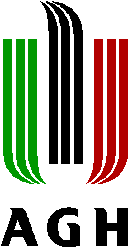
\includegraphics{img/agh.png}

        \vspace{1cm}

        \large\textsc{STUDIA PODYPLOMOWE
        \\ANALIZA DANYCH – DATA SCIENCE}

        \vspace{1cm}
        \large{Projekt dyplomowy}

        \vspace{0.8cm}

        \textbf{Analysis of Prediction Power of Information about Payment Delay to Forecast Financial Problems}

        \vspace{1.5cm}

        \textbf{Autor}\\
        \textbf{mgr inż. Konrad J. Gródek}

        \vspace{0.8cm}
        \textbf{Opiekun Projektu}\\
        \textbf{dr inż. Robert Marcjan}


        \vfill

        \large{Kraków, 2023}

        \end{center}
    \end{titlepage}

\pagebreak


\begin{abstract}
\vspace{1cm}

The project will focus on information about bill payment experiences - information coming from various
sources, from companies that report the bill issue and payment day. The bill may be paid with certain
delay or ahead of time. In the latter case the term “delay” makes no lexical sense, but in order to keep consistent naming,
the difference in days between issue and payment will be hereinafter referred to as delay,
which may take negative value to picture the bill being paid in advance.\par
The first step will be to assess the quality of the sources and to choose those, where the information is reliable and have potential for further analysis.
The goal of the second part is to find proved connections between the pay-delay details and the
financial issues that had happened afterwards. The details of the payment will cover attributes like the
delay in days, the amount and the time-line of the payments. It is important to explore also the tendencies
that occur for these numbers over time. The analysis must also take into consideration the gradual
nature of the “financial problems”, which take one of few severity levels, from collection notice to
bankruptcy.\par
The analysis will be performed on data collected by Crif AG from Zurich, leading economic information
bureau in Switzerland. The data, neither of the bill issuer nor bill payer, must not be revealed in the final
project documentation.

\end{abstract}

\pagebreak

\tableofcontents

\pagebreak

\section{Introduction}

This section will provide more elaborate description of the problem and will provide more information on the data, which will be used in the project.

\subsection{The problem}

Crif AG is a Swiss economic information bureau delivering solutions for clients interested in checking creditworthiness of both private and corporate individuals.
For number of years the company was collecting information about paid bills issued by Crif's customers.
Till now the information was not included in the procedures of calculating probability of default (so-called \textit{scoring}).
The aim of this work is to explore the potential hidden in the data to support process of evaluating creditworthiness.
In order to do that, certain attributes of the data must be explored and confronted with history of negative payment information (debts).
As a result, statistical evidence will prove - or not - existence of correlation between those attributes (variables)
and the probability of default. The correlation must be backed up by plausible causation.\par

It is important to stress that the analysis will be performed exclusively on data recorded for private persons.\par

\subsection{The data}

The data in scope of the analysis can be divided into three types: payment delay, debt and legal entity information.

\subsubsection{Payment delay}

As it was already mentioned, the \textbf{payment delay} term may be misleading.
What is understood by this term can be more precisely explained as \textbf{the performance of paying the bill}.
Once issued, the bill may be paid in advance, on time or with a certain delay.\par
\vspace{5pt}
The \textbf{payment delay} comes with the following attributes:
\begin{itemize}
    \item Bill issue date
    \item The delay measured as the number of days between the issue and payment dates. May be negative.
    \item The billed amount. May be missing (unknown)
    \item The identification of the bill issuer (the \textit{source})
    \item The industrial sector of the bill issuer
    \item The identification of the bill payer (also related to as \textit{legal entity})
\end{itemize}

Except invoiced amount, all the listed attributes are obligatorily present in the data set.
The industrial sector of the bill issuer may be unknown, but is still delivered as separate category.

\subsubsection{Debt}
\label{section:intro-debt}

The \textbf{debt} is a recorded negative payment experience.
It has certain severity and validity period.
The list of attributes:
\begin{itemize}
    \item Validity period: start and end date (note that the second may be in the future)
    \item Amount owned - it will not be used in the analysis
    \item Severity
    \item The identification of the debtor, which will be used to connect to payment-delay set
\end{itemize}

All listed attributes are obligatorily present in the data set.\par
Severity of the debt comes as four categories, marked with numbers 1 to 4. The higher the number is,
the more severe the debt information is. Not to get into too much details:
1 represents first step of vindication process whereas 4 is reserved for cases when
debtor persistently refuses to repay the liability.\par
For sake of the analysis, the severity will be split into two groups, where existence of a debt from given group comes with:
\begin{itemize}
    \item mild risk of incorrect payment behavior (1 - 2),
    \item high risk of incorrect payment behavior (3 - 4).
\end{itemize}

\subsubsection{Legal entity}

Only sociodemographic information is accessible for sake of this analysis. 
This includes only very limited set of attributes:

\begin{itemize}
    \item Age (rounded to full years)
    \item Gender
\end{itemize}

Each of the listed attributes may appear undefined (none of them is obligatory).\par 

\textbf{Analysing sociodemographic data is out of scope for this analysis.
The goal is to find negative patters in payment behavior, not to link it to particular age or gender}

\subsection{The quality challenge}
\label{section:intro-quality-challenge}

One of the challenges to be faced in order to answer on the formulated problem is how to deal with the source quality issues.
The data is coming from various sources and the quality of delivery is often questionable.
The exploratory part of the analysis will focus on pointing out the differences between the sources.\par
What measurements shall be used to calculate the quality of the source? The following ideas will be explored:
\begin{itemize}
    \item \textbf{Number of recorded payments}. The simplest - but often misleading - way to asses the usefulness of the data source. Obviously, the more records the better, but if the data is not reliable, the large volume will not make it better.
    \item \textbf{Average number of paid bills per person}. From the two sources the one providing longer history of payments per person will most likely be more useful than the one providing single payments.
    \item \textbf{Ratio of missing values and outliers.} Surely high ratio of the data, which remain undefined (applies mostly to sociodemographic attributes) makes the source less attractive. The same applies to source with high number of unreliable data
    \item \textbf{Overrepresentation of "0-delay" records}. If the source reports that the bills are paid exactly on time by vast majority of payers, its predictive power will be close to zero.
    \item \textbf{Data continuity versus clustered information}. Partialy related to the above. There is nothing bad if the source reports the delay in certain periods (e.g. every week or month), but in such a case the source may be treated differently from the one that reports in more continuous manner.
    \item \textbf{Variability}. Except continuity, a desired situation is to have more variable data, spanning over longer periods, including high and low amounts, scrupulous payers as well as those neglecting liabilities.
\end{itemize}

\pagebreak

\subsection{The technology}

As main coding language, \textbf{python} was used.

\par The amount of data to be processed requires solutions dedicated to efficiently process so-called columnar data.
Legal constraints requires this analysis to be performed on typical laptop (AMD Ryzen 7 @ 2.3 GHz, 16 GB RAM, Windows 10).
Among variety of available products the following were considered:
\begin{itemize}
    \item \textbf{Apache Spark} is an industry-standard engine dedicated to process vast amount of data. It is especially efficient whenever the problem may be distributed over multiple machines.
    \item \textbf{DuckDB} is pretty new serverless SQL database management system that is optimized to process tabular datasets, allowing to efficiently join and aggregate large tables.
    \item \textbf{Apache Arrow} provides effectively in-memory operations for analytical purposes. It comes with standardized columnar memory format, which is optimized for efficiantly process large amount of records.
\end{itemize}

It was decided to use \textbf{Apache Arrow}.
The main factor, which supports this choice, is optimization on in-memory operations and ease of use - required solely installation of python package.
DuckDB, although equally easy to use and pretty powerful in running queries directly on parquet files, is still immature technology.
Spark would be chosen if the analysis could be done in cloud, which was not possible.
Surely it may be run on a single machine, but it would not show its true potential.

\par The below list presents other libraries / technologies used during the project.
\begin{itemize}
    \item \textbf{Apache Parquet} to store intermediate data on disk.
    \item \textbf{Pandas} to collect aggregated data, to display and generate LaTeX tables.
    \item \textbf{Matplotlib} to produce all visualisations and store them as PGF files.
    \item \textbf{Jupyter Notebook} as supporting tool for analysis (it was not used to prepare any output)
\end{itemize}

\section{Exploratory analysis}

The goal of the exploratory analysis is to get to know data better.
It should consist of checking metrics that gives an idea on quantity (how many records are there? what is the count of groups of records?)
as well as quality (are the records meet criteria that will not cause potential errors in further analysis?)

\subsection{The data overview}

The data is composed of nearly 180 million payment observations and over 8 million debts.
Table\ \ref{tab:000_overview_whole_dataset} presents the very basic statistics on the whole set. \par
\begin{table}[htbp!] \centering
\caption{Whole data set overview}
\label{tab:000_overview_whole_dataset}
\begin{tabular}{rrrrr}
\\[-1.8ex]\hline\hline \\[-1.8ex]
All records count & Entities count & Avg delay (days) & Delay = 0 (\%) & Non-empty amount (\%) \\
\midrule
177385038 & 6963998 & -2.29 & 55.05 & 58.33 \\
\bottomrule
\end{tabular}
\end{table}

First conclusions are:
\begin{itemize}
    \item Average delay of paid bills is negative, so in general the data set does provide more optimistic data (bills paid in advance) than negative (delays in payments)
    \item Significant part of the payment records (over half of it) shows the bills to be paid exactly on time.
    \item The amount is quite often unknown
\end{itemize}

To have better view on characteristic of the most important attribute: the delay in days, a histogram is presented on figure \ref{fig:001_delay_days_hist}.
The y-axis was limited to maximum 10\% as the 55\% peak in delay-days=0 makes the chart unreadable.
There is one more peak in observations, placed at -30 days.
As later analysis will show, this is an effect of two sources delivering abundance of records with fixed value of -30 between the issue date and payment date.\par

\begin{figure}[htbp!]
    \begin{center}
        %% Creator: Matplotlib, PGF backend
%%
%% To include the figure in your LaTeX document, write
%%   \input{<filename>.pgf}
%%
%% Make sure the required packages are loaded in your preamble
%%   \usepackage{pgf}
%%
%% Also ensure that all the required font packages are loaded; for instance,
%% the lmodern package is sometimes necessary when using math font.
%%   \usepackage{lmodern}
%%
%% Figures using additional raster images can only be included by \input if
%% they are in the same directory as the main LaTeX file. For loading figures
%% from other directories you can use the `import` package
%%   \usepackage{import}
%%
%% and then include the figures with
%%   \import{<path to file>}{<filename>.pgf}
%%
%% Matplotlib used the following preamble
%%   
%%   \makeatletter\@ifpackageloaded{underscore}{}{\usepackage[strings]{underscore}}\makeatother
%%
\begingroup%
\makeatletter%
\begin{pgfpicture}%
\pgfpathrectangle{\pgfpointorigin}{\pgfqpoint{6.500000in}{4.000000in}}%
\pgfusepath{use as bounding box, clip}%
\begin{pgfscope}%
\pgfsetbuttcap%
\pgfsetmiterjoin%
\definecolor{currentfill}{rgb}{1.000000,1.000000,1.000000}%
\pgfsetfillcolor{currentfill}%
\pgfsetlinewidth{0.000000pt}%
\definecolor{currentstroke}{rgb}{1.000000,1.000000,1.000000}%
\pgfsetstrokecolor{currentstroke}%
\pgfsetdash{}{0pt}%
\pgfpathmoveto{\pgfqpoint{0.000000in}{0.000000in}}%
\pgfpathlineto{\pgfqpoint{6.500000in}{0.000000in}}%
\pgfpathlineto{\pgfqpoint{6.500000in}{4.000000in}}%
\pgfpathlineto{\pgfqpoint{0.000000in}{4.000000in}}%
\pgfpathlineto{\pgfqpoint{0.000000in}{0.000000in}}%
\pgfpathclose%
\pgfusepath{fill}%
\end{pgfscope}%
\begin{pgfscope}%
\pgfsetbuttcap%
\pgfsetmiterjoin%
\definecolor{currentfill}{rgb}{1.000000,1.000000,1.000000}%
\pgfsetfillcolor{currentfill}%
\pgfsetlinewidth{0.000000pt}%
\definecolor{currentstroke}{rgb}{0.000000,0.000000,0.000000}%
\pgfsetstrokecolor{currentstroke}%
\pgfsetstrokeopacity{0.000000}%
\pgfsetdash{}{0pt}%
\pgfpathmoveto{\pgfqpoint{0.812500in}{0.440000in}}%
\pgfpathlineto{\pgfqpoint{5.850000in}{0.440000in}}%
\pgfpathlineto{\pgfqpoint{5.850000in}{3.520000in}}%
\pgfpathlineto{\pgfqpoint{0.812500in}{3.520000in}}%
\pgfpathlineto{\pgfqpoint{0.812500in}{0.440000in}}%
\pgfpathclose%
\pgfusepath{fill}%
\end{pgfscope}%
\begin{pgfscope}%
\pgfpathrectangle{\pgfqpoint{0.812500in}{0.440000in}}{\pgfqpoint{5.037500in}{3.080000in}}%
\pgfusepath{clip}%
\pgfsetbuttcap%
\pgfsetmiterjoin%
\definecolor{currentfill}{rgb}{0.501961,0.501961,0.501961}%
\pgfsetfillcolor{currentfill}%
\pgfsetlinewidth{1.003750pt}%
\definecolor{currentstroke}{rgb}{1.000000,1.000000,1.000000}%
\pgfsetstrokecolor{currentstroke}%
\pgfsetdash{}{0pt}%
\pgfpathmoveto{\pgfqpoint{0.702813in}{0.440000in}}%
\pgfpathlineto{\pgfqpoint{0.759688in}{0.440000in}}%
\pgfpathlineto{\pgfqpoint{0.759688in}{0.523145in}}%
\pgfpathlineto{\pgfqpoint{0.702813in}{0.523145in}}%
\pgfpathlineto{\pgfqpoint{0.702813in}{0.440000in}}%
\pgfpathclose%
\pgfusepath{stroke,fill}%
\end{pgfscope}%
\begin{pgfscope}%
\pgfpathrectangle{\pgfqpoint{0.812500in}{0.440000in}}{\pgfqpoint{5.037500in}{3.080000in}}%
\pgfusepath{clip}%
\pgfsetbuttcap%
\pgfsetmiterjoin%
\definecolor{currentfill}{rgb}{0.501961,0.501961,0.501961}%
\pgfsetfillcolor{currentfill}%
\pgfsetlinewidth{1.003750pt}%
\definecolor{currentstroke}{rgb}{1.000000,1.000000,1.000000}%
\pgfsetstrokecolor{currentstroke}%
\pgfsetdash{}{0pt}%
\pgfpathmoveto{\pgfqpoint{0.784062in}{0.440000in}}%
\pgfpathlineto{\pgfqpoint{0.840938in}{0.440000in}}%
\pgfpathlineto{\pgfqpoint{0.840938in}{0.451679in}}%
\pgfpathlineto{\pgfqpoint{0.784062in}{0.451679in}}%
\pgfpathlineto{\pgfqpoint{0.784062in}{0.440000in}}%
\pgfpathclose%
\pgfusepath{stroke,fill}%
\end{pgfscope}%
\begin{pgfscope}%
\pgfpathrectangle{\pgfqpoint{0.812500in}{0.440000in}}{\pgfqpoint{5.037500in}{3.080000in}}%
\pgfusepath{clip}%
\pgfsetbuttcap%
\pgfsetmiterjoin%
\definecolor{currentfill}{rgb}{0.501961,0.501961,0.501961}%
\pgfsetfillcolor{currentfill}%
\pgfsetlinewidth{1.003750pt}%
\definecolor{currentstroke}{rgb}{1.000000,1.000000,1.000000}%
\pgfsetstrokecolor{currentstroke}%
\pgfsetdash{}{0pt}%
\pgfpathmoveto{\pgfqpoint{0.865313in}{0.440000in}}%
\pgfpathlineto{\pgfqpoint{0.922188in}{0.440000in}}%
\pgfpathlineto{\pgfqpoint{0.922188in}{0.450233in}}%
\pgfpathlineto{\pgfqpoint{0.865313in}{0.450233in}}%
\pgfpathlineto{\pgfqpoint{0.865313in}{0.440000in}}%
\pgfpathclose%
\pgfusepath{stroke,fill}%
\end{pgfscope}%
\begin{pgfscope}%
\pgfpathrectangle{\pgfqpoint{0.812500in}{0.440000in}}{\pgfqpoint{5.037500in}{3.080000in}}%
\pgfusepath{clip}%
\pgfsetbuttcap%
\pgfsetmiterjoin%
\definecolor{currentfill}{rgb}{0.501961,0.501961,0.501961}%
\pgfsetfillcolor{currentfill}%
\pgfsetlinewidth{1.003750pt}%
\definecolor{currentstroke}{rgb}{1.000000,1.000000,1.000000}%
\pgfsetstrokecolor{currentstroke}%
\pgfsetdash{}{0pt}%
\pgfpathmoveto{\pgfqpoint{0.946562in}{0.440000in}}%
\pgfpathlineto{\pgfqpoint{1.003438in}{0.440000in}}%
\pgfpathlineto{\pgfqpoint{1.003438in}{2.547199in}}%
\pgfpathlineto{\pgfqpoint{0.946562in}{2.547199in}}%
\pgfpathlineto{\pgfqpoint{0.946562in}{0.440000in}}%
\pgfpathclose%
\pgfusepath{stroke,fill}%
\end{pgfscope}%
\begin{pgfscope}%
\pgfpathrectangle{\pgfqpoint{0.812500in}{0.440000in}}{\pgfqpoint{5.037500in}{3.080000in}}%
\pgfusepath{clip}%
\pgfsetbuttcap%
\pgfsetmiterjoin%
\definecolor{currentfill}{rgb}{0.501961,0.501961,0.501961}%
\pgfsetfillcolor{currentfill}%
\pgfsetlinewidth{1.003750pt}%
\definecolor{currentstroke}{rgb}{1.000000,1.000000,1.000000}%
\pgfsetstrokecolor{currentstroke}%
\pgfsetdash{}{0pt}%
\pgfpathmoveto{\pgfqpoint{1.027813in}{0.440000in}}%
\pgfpathlineto{\pgfqpoint{1.084688in}{0.440000in}}%
\pgfpathlineto{\pgfqpoint{1.084688in}{0.631576in}}%
\pgfpathlineto{\pgfqpoint{1.027813in}{0.631576in}}%
\pgfpathlineto{\pgfqpoint{1.027813in}{0.440000in}}%
\pgfpathclose%
\pgfusepath{stroke,fill}%
\end{pgfscope}%
\begin{pgfscope}%
\pgfpathrectangle{\pgfqpoint{0.812500in}{0.440000in}}{\pgfqpoint{5.037500in}{3.080000in}}%
\pgfusepath{clip}%
\pgfsetbuttcap%
\pgfsetmiterjoin%
\definecolor{currentfill}{rgb}{0.501961,0.501961,0.501961}%
\pgfsetfillcolor{currentfill}%
\pgfsetlinewidth{1.003750pt}%
\definecolor{currentstroke}{rgb}{1.000000,1.000000,1.000000}%
\pgfsetstrokecolor{currentstroke}%
\pgfsetdash{}{0pt}%
\pgfpathmoveto{\pgfqpoint{1.109063in}{0.440000in}}%
\pgfpathlineto{\pgfqpoint{1.165938in}{0.440000in}}%
\pgfpathlineto{\pgfqpoint{1.165938in}{0.504673in}}%
\pgfpathlineto{\pgfqpoint{1.109063in}{0.504673in}}%
\pgfpathlineto{\pgfqpoint{1.109063in}{0.440000in}}%
\pgfpathclose%
\pgfusepath{stroke,fill}%
\end{pgfscope}%
\begin{pgfscope}%
\pgfpathrectangle{\pgfqpoint{0.812500in}{0.440000in}}{\pgfqpoint{5.037500in}{3.080000in}}%
\pgfusepath{clip}%
\pgfsetbuttcap%
\pgfsetmiterjoin%
\definecolor{currentfill}{rgb}{0.501961,0.501961,0.501961}%
\pgfsetfillcolor{currentfill}%
\pgfsetlinewidth{1.003750pt}%
\definecolor{currentstroke}{rgb}{1.000000,1.000000,1.000000}%
\pgfsetstrokecolor{currentstroke}%
\pgfsetdash{}{0pt}%
\pgfpathmoveto{\pgfqpoint{1.190313in}{0.440000in}}%
\pgfpathlineto{\pgfqpoint{1.247188in}{0.440000in}}%
\pgfpathlineto{\pgfqpoint{1.247188in}{0.500378in}}%
\pgfpathlineto{\pgfqpoint{1.190313in}{0.500378in}}%
\pgfpathlineto{\pgfqpoint{1.190313in}{0.440000in}}%
\pgfpathclose%
\pgfusepath{stroke,fill}%
\end{pgfscope}%
\begin{pgfscope}%
\pgfpathrectangle{\pgfqpoint{0.812500in}{0.440000in}}{\pgfqpoint{5.037500in}{3.080000in}}%
\pgfusepath{clip}%
\pgfsetbuttcap%
\pgfsetmiterjoin%
\definecolor{currentfill}{rgb}{0.501961,0.501961,0.501961}%
\pgfsetfillcolor{currentfill}%
\pgfsetlinewidth{1.003750pt}%
\definecolor{currentstroke}{rgb}{1.000000,1.000000,1.000000}%
\pgfsetstrokecolor{currentstroke}%
\pgfsetdash{}{0pt}%
\pgfpathmoveto{\pgfqpoint{1.271562in}{0.440000in}}%
\pgfpathlineto{\pgfqpoint{1.328438in}{0.440000in}}%
\pgfpathlineto{\pgfqpoint{1.328438in}{0.507861in}}%
\pgfpathlineto{\pgfqpoint{1.271562in}{0.507861in}}%
\pgfpathlineto{\pgfqpoint{1.271562in}{0.440000in}}%
\pgfpathclose%
\pgfusepath{stroke,fill}%
\end{pgfscope}%
\begin{pgfscope}%
\pgfpathrectangle{\pgfqpoint{0.812500in}{0.440000in}}{\pgfqpoint{5.037500in}{3.080000in}}%
\pgfusepath{clip}%
\pgfsetbuttcap%
\pgfsetmiterjoin%
\definecolor{currentfill}{rgb}{0.501961,0.501961,0.501961}%
\pgfsetfillcolor{currentfill}%
\pgfsetlinewidth{1.003750pt}%
\definecolor{currentstroke}{rgb}{1.000000,1.000000,1.000000}%
\pgfsetstrokecolor{currentstroke}%
\pgfsetdash{}{0pt}%
\pgfpathmoveto{\pgfqpoint{1.352812in}{0.440000in}}%
\pgfpathlineto{\pgfqpoint{1.409688in}{0.440000in}}%
\pgfpathlineto{\pgfqpoint{1.409688in}{0.520801in}}%
\pgfpathlineto{\pgfqpoint{1.352812in}{0.520801in}}%
\pgfpathlineto{\pgfqpoint{1.352812in}{0.440000in}}%
\pgfpathclose%
\pgfusepath{stroke,fill}%
\end{pgfscope}%
\begin{pgfscope}%
\pgfpathrectangle{\pgfqpoint{0.812500in}{0.440000in}}{\pgfqpoint{5.037500in}{3.080000in}}%
\pgfusepath{clip}%
\pgfsetbuttcap%
\pgfsetmiterjoin%
\definecolor{currentfill}{rgb}{0.501961,0.501961,0.501961}%
\pgfsetfillcolor{currentfill}%
\pgfsetlinewidth{1.003750pt}%
\definecolor{currentstroke}{rgb}{1.000000,1.000000,1.000000}%
\pgfsetstrokecolor{currentstroke}%
\pgfsetdash{}{0pt}%
\pgfpathmoveto{\pgfqpoint{1.434063in}{0.440000in}}%
\pgfpathlineto{\pgfqpoint{1.490938in}{0.440000in}}%
\pgfpathlineto{\pgfqpoint{1.490938in}{0.531193in}}%
\pgfpathlineto{\pgfqpoint{1.434063in}{0.531193in}}%
\pgfpathlineto{\pgfqpoint{1.434063in}{0.440000in}}%
\pgfpathclose%
\pgfusepath{stroke,fill}%
\end{pgfscope}%
\begin{pgfscope}%
\pgfpathrectangle{\pgfqpoint{0.812500in}{0.440000in}}{\pgfqpoint{5.037500in}{3.080000in}}%
\pgfusepath{clip}%
\pgfsetbuttcap%
\pgfsetmiterjoin%
\definecolor{currentfill}{rgb}{0.501961,0.501961,0.501961}%
\pgfsetfillcolor{currentfill}%
\pgfsetlinewidth{1.003750pt}%
\definecolor{currentstroke}{rgb}{1.000000,1.000000,1.000000}%
\pgfsetstrokecolor{currentstroke}%
\pgfsetdash{}{0pt}%
\pgfpathmoveto{\pgfqpoint{1.515313in}{0.440000in}}%
\pgfpathlineto{\pgfqpoint{1.572188in}{0.440000in}}%
\pgfpathlineto{\pgfqpoint{1.572188in}{0.544713in}}%
\pgfpathlineto{\pgfqpoint{1.515313in}{0.544713in}}%
\pgfpathlineto{\pgfqpoint{1.515313in}{0.440000in}}%
\pgfpathclose%
\pgfusepath{stroke,fill}%
\end{pgfscope}%
\begin{pgfscope}%
\pgfpathrectangle{\pgfqpoint{0.812500in}{0.440000in}}{\pgfqpoint{5.037500in}{3.080000in}}%
\pgfusepath{clip}%
\pgfsetbuttcap%
\pgfsetmiterjoin%
\definecolor{currentfill}{rgb}{0.501961,0.501961,0.501961}%
\pgfsetfillcolor{currentfill}%
\pgfsetlinewidth{1.003750pt}%
\definecolor{currentstroke}{rgb}{1.000000,1.000000,1.000000}%
\pgfsetstrokecolor{currentstroke}%
\pgfsetdash{}{0pt}%
\pgfpathmoveto{\pgfqpoint{1.596563in}{0.440000in}}%
\pgfpathlineto{\pgfqpoint{1.653438in}{0.440000in}}%
\pgfpathlineto{\pgfqpoint{1.653438in}{0.532393in}}%
\pgfpathlineto{\pgfqpoint{1.596563in}{0.532393in}}%
\pgfpathlineto{\pgfqpoint{1.596563in}{0.440000in}}%
\pgfpathclose%
\pgfusepath{stroke,fill}%
\end{pgfscope}%
\begin{pgfscope}%
\pgfpathrectangle{\pgfqpoint{0.812500in}{0.440000in}}{\pgfqpoint{5.037500in}{3.080000in}}%
\pgfusepath{clip}%
\pgfsetbuttcap%
\pgfsetmiterjoin%
\definecolor{currentfill}{rgb}{0.501961,0.501961,0.501961}%
\pgfsetfillcolor{currentfill}%
\pgfsetlinewidth{1.003750pt}%
\definecolor{currentstroke}{rgb}{1.000000,1.000000,1.000000}%
\pgfsetstrokecolor{currentstroke}%
\pgfsetdash{}{0pt}%
\pgfpathmoveto{\pgfqpoint{1.677812in}{0.440000in}}%
\pgfpathlineto{\pgfqpoint{1.734688in}{0.440000in}}%
\pgfpathlineto{\pgfqpoint{1.734688in}{0.528790in}}%
\pgfpathlineto{\pgfqpoint{1.677812in}{0.528790in}}%
\pgfpathlineto{\pgfqpoint{1.677812in}{0.440000in}}%
\pgfpathclose%
\pgfusepath{stroke,fill}%
\end{pgfscope}%
\begin{pgfscope}%
\pgfpathrectangle{\pgfqpoint{0.812500in}{0.440000in}}{\pgfqpoint{5.037500in}{3.080000in}}%
\pgfusepath{clip}%
\pgfsetbuttcap%
\pgfsetmiterjoin%
\definecolor{currentfill}{rgb}{0.501961,0.501961,0.501961}%
\pgfsetfillcolor{currentfill}%
\pgfsetlinewidth{1.003750pt}%
\definecolor{currentstroke}{rgb}{1.000000,1.000000,1.000000}%
\pgfsetstrokecolor{currentstroke}%
\pgfsetdash{}{0pt}%
\pgfpathmoveto{\pgfqpoint{1.759062in}{0.440000in}}%
\pgfpathlineto{\pgfqpoint{1.815938in}{0.440000in}}%
\pgfpathlineto{\pgfqpoint{1.815938in}{0.589075in}}%
\pgfpathlineto{\pgfqpoint{1.759062in}{0.589075in}}%
\pgfpathlineto{\pgfqpoint{1.759062in}{0.440000in}}%
\pgfpathclose%
\pgfusepath{stroke,fill}%
\end{pgfscope}%
\begin{pgfscope}%
\pgfpathrectangle{\pgfqpoint{0.812500in}{0.440000in}}{\pgfqpoint{5.037500in}{3.080000in}}%
\pgfusepath{clip}%
\pgfsetbuttcap%
\pgfsetmiterjoin%
\definecolor{currentfill}{rgb}{0.501961,0.501961,0.501961}%
\pgfsetfillcolor{currentfill}%
\pgfsetlinewidth{1.003750pt}%
\definecolor{currentstroke}{rgb}{1.000000,1.000000,1.000000}%
\pgfsetstrokecolor{currentstroke}%
\pgfsetdash{}{0pt}%
\pgfpathmoveto{\pgfqpoint{1.840313in}{0.440000in}}%
\pgfpathlineto{\pgfqpoint{1.897188in}{0.440000in}}%
\pgfpathlineto{\pgfqpoint{1.897188in}{0.551424in}}%
\pgfpathlineto{\pgfqpoint{1.840313in}{0.551424in}}%
\pgfpathlineto{\pgfqpoint{1.840313in}{0.440000in}}%
\pgfpathclose%
\pgfusepath{stroke,fill}%
\end{pgfscope}%
\begin{pgfscope}%
\pgfpathrectangle{\pgfqpoint{0.812500in}{0.440000in}}{\pgfqpoint{5.037500in}{3.080000in}}%
\pgfusepath{clip}%
\pgfsetbuttcap%
\pgfsetmiterjoin%
\definecolor{currentfill}{rgb}{0.501961,0.501961,0.501961}%
\pgfsetfillcolor{currentfill}%
\pgfsetlinewidth{1.003750pt}%
\definecolor{currentstroke}{rgb}{1.000000,1.000000,1.000000}%
\pgfsetstrokecolor{currentstroke}%
\pgfsetdash{}{0pt}%
\pgfpathmoveto{\pgfqpoint{1.921563in}{0.440000in}}%
\pgfpathlineto{\pgfqpoint{1.978438in}{0.440000in}}%
\pgfpathlineto{\pgfqpoint{1.978438in}{0.565253in}}%
\pgfpathlineto{\pgfqpoint{1.921563in}{0.565253in}}%
\pgfpathlineto{\pgfqpoint{1.921563in}{0.440000in}}%
\pgfpathclose%
\pgfusepath{stroke,fill}%
\end{pgfscope}%
\begin{pgfscope}%
\pgfpathrectangle{\pgfqpoint{0.812500in}{0.440000in}}{\pgfqpoint{5.037500in}{3.080000in}}%
\pgfusepath{clip}%
\pgfsetbuttcap%
\pgfsetmiterjoin%
\definecolor{currentfill}{rgb}{0.501961,0.501961,0.501961}%
\pgfsetfillcolor{currentfill}%
\pgfsetlinewidth{1.003750pt}%
\definecolor{currentstroke}{rgb}{1.000000,1.000000,1.000000}%
\pgfsetstrokecolor{currentstroke}%
\pgfsetdash{}{0pt}%
\pgfpathmoveto{\pgfqpoint{2.002813in}{0.440000in}}%
\pgfpathlineto{\pgfqpoint{2.059688in}{0.440000in}}%
\pgfpathlineto{\pgfqpoint{2.059688in}{0.621353in}}%
\pgfpathlineto{\pgfqpoint{2.002813in}{0.621353in}}%
\pgfpathlineto{\pgfqpoint{2.002813in}{0.440000in}}%
\pgfpathclose%
\pgfusepath{stroke,fill}%
\end{pgfscope}%
\begin{pgfscope}%
\pgfpathrectangle{\pgfqpoint{0.812500in}{0.440000in}}{\pgfqpoint{5.037500in}{3.080000in}}%
\pgfusepath{clip}%
\pgfsetbuttcap%
\pgfsetmiterjoin%
\definecolor{currentfill}{rgb}{0.501961,0.501961,0.501961}%
\pgfsetfillcolor{currentfill}%
\pgfsetlinewidth{1.003750pt}%
\definecolor{currentstroke}{rgb}{1.000000,1.000000,1.000000}%
\pgfsetstrokecolor{currentstroke}%
\pgfsetdash{}{0pt}%
\pgfpathmoveto{\pgfqpoint{2.084062in}{0.440000in}}%
\pgfpathlineto{\pgfqpoint{2.140938in}{0.440000in}}%
\pgfpathlineto{\pgfqpoint{2.140938in}{0.637323in}}%
\pgfpathlineto{\pgfqpoint{2.084062in}{0.637323in}}%
\pgfpathlineto{\pgfqpoint{2.084062in}{0.440000in}}%
\pgfpathclose%
\pgfusepath{stroke,fill}%
\end{pgfscope}%
\begin{pgfscope}%
\pgfpathrectangle{\pgfqpoint{0.812500in}{0.440000in}}{\pgfqpoint{5.037500in}{3.080000in}}%
\pgfusepath{clip}%
\pgfsetbuttcap%
\pgfsetmiterjoin%
\definecolor{currentfill}{rgb}{0.501961,0.501961,0.501961}%
\pgfsetfillcolor{currentfill}%
\pgfsetlinewidth{1.003750pt}%
\definecolor{currentstroke}{rgb}{1.000000,1.000000,1.000000}%
\pgfsetstrokecolor{currentstroke}%
\pgfsetdash{}{0pt}%
\pgfpathmoveto{\pgfqpoint{2.165313in}{0.440000in}}%
\pgfpathlineto{\pgfqpoint{2.222188in}{0.440000in}}%
\pgfpathlineto{\pgfqpoint{2.222188in}{0.638481in}}%
\pgfpathlineto{\pgfqpoint{2.165313in}{0.638481in}}%
\pgfpathlineto{\pgfqpoint{2.165313in}{0.440000in}}%
\pgfpathclose%
\pgfusepath{stroke,fill}%
\end{pgfscope}%
\begin{pgfscope}%
\pgfpathrectangle{\pgfqpoint{0.812500in}{0.440000in}}{\pgfqpoint{5.037500in}{3.080000in}}%
\pgfusepath{clip}%
\pgfsetbuttcap%
\pgfsetmiterjoin%
\definecolor{currentfill}{rgb}{0.501961,0.501961,0.501961}%
\pgfsetfillcolor{currentfill}%
\pgfsetlinewidth{1.003750pt}%
\definecolor{currentstroke}{rgb}{1.000000,1.000000,1.000000}%
\pgfsetstrokecolor{currentstroke}%
\pgfsetdash{}{0pt}%
\pgfpathmoveto{\pgfqpoint{2.246563in}{0.440000in}}%
\pgfpathlineto{\pgfqpoint{2.303438in}{0.440000in}}%
\pgfpathlineto{\pgfqpoint{2.303438in}{0.673233in}}%
\pgfpathlineto{\pgfqpoint{2.246563in}{0.673233in}}%
\pgfpathlineto{\pgfqpoint{2.246563in}{0.440000in}}%
\pgfpathclose%
\pgfusepath{stroke,fill}%
\end{pgfscope}%
\begin{pgfscope}%
\pgfpathrectangle{\pgfqpoint{0.812500in}{0.440000in}}{\pgfqpoint{5.037500in}{3.080000in}}%
\pgfusepath{clip}%
\pgfsetbuttcap%
\pgfsetmiterjoin%
\definecolor{currentfill}{rgb}{0.501961,0.501961,0.501961}%
\pgfsetfillcolor{currentfill}%
\pgfsetlinewidth{1.003750pt}%
\definecolor{currentstroke}{rgb}{1.000000,1.000000,1.000000}%
\pgfsetstrokecolor{currentstroke}%
\pgfsetdash{}{0pt}%
\pgfpathmoveto{\pgfqpoint{2.327812in}{0.440000in}}%
\pgfpathlineto{\pgfqpoint{2.384688in}{0.440000in}}%
\pgfpathlineto{\pgfqpoint{2.384688in}{0.676981in}}%
\pgfpathlineto{\pgfqpoint{2.327812in}{0.676981in}}%
\pgfpathlineto{\pgfqpoint{2.327812in}{0.440000in}}%
\pgfpathclose%
\pgfusepath{stroke,fill}%
\end{pgfscope}%
\begin{pgfscope}%
\pgfpathrectangle{\pgfqpoint{0.812500in}{0.440000in}}{\pgfqpoint{5.037500in}{3.080000in}}%
\pgfusepath{clip}%
\pgfsetbuttcap%
\pgfsetmiterjoin%
\definecolor{currentfill}{rgb}{0.501961,0.501961,0.501961}%
\pgfsetfillcolor{currentfill}%
\pgfsetlinewidth{1.003750pt}%
\definecolor{currentstroke}{rgb}{1.000000,1.000000,1.000000}%
\pgfsetstrokecolor{currentstroke}%
\pgfsetdash{}{0pt}%
\pgfpathmoveto{\pgfqpoint{2.409063in}{0.440000in}}%
\pgfpathlineto{\pgfqpoint{2.465938in}{0.440000in}}%
\pgfpathlineto{\pgfqpoint{2.465938in}{0.674390in}}%
\pgfpathlineto{\pgfqpoint{2.409063in}{0.674390in}}%
\pgfpathlineto{\pgfqpoint{2.409063in}{0.440000in}}%
\pgfpathclose%
\pgfusepath{stroke,fill}%
\end{pgfscope}%
\begin{pgfscope}%
\pgfpathrectangle{\pgfqpoint{0.812500in}{0.440000in}}{\pgfqpoint{5.037500in}{3.080000in}}%
\pgfusepath{clip}%
\pgfsetbuttcap%
\pgfsetmiterjoin%
\definecolor{currentfill}{rgb}{0.501961,0.501961,0.501961}%
\pgfsetfillcolor{currentfill}%
\pgfsetlinewidth{1.003750pt}%
\definecolor{currentstroke}{rgb}{1.000000,1.000000,1.000000}%
\pgfsetstrokecolor{currentstroke}%
\pgfsetdash{}{0pt}%
\pgfpathmoveto{\pgfqpoint{2.490312in}{0.440000in}}%
\pgfpathlineto{\pgfqpoint{2.547188in}{0.440000in}}%
\pgfpathlineto{\pgfqpoint{2.547188in}{0.667044in}}%
\pgfpathlineto{\pgfqpoint{2.490312in}{0.667044in}}%
\pgfpathlineto{\pgfqpoint{2.490312in}{0.440000in}}%
\pgfpathclose%
\pgfusepath{stroke,fill}%
\end{pgfscope}%
\begin{pgfscope}%
\pgfpathrectangle{\pgfqpoint{0.812500in}{0.440000in}}{\pgfqpoint{5.037500in}{3.080000in}}%
\pgfusepath{clip}%
\pgfsetbuttcap%
\pgfsetmiterjoin%
\definecolor{currentfill}{rgb}{0.501961,0.501961,0.501961}%
\pgfsetfillcolor{currentfill}%
\pgfsetlinewidth{1.003750pt}%
\definecolor{currentstroke}{rgb}{1.000000,1.000000,1.000000}%
\pgfsetstrokecolor{currentstroke}%
\pgfsetdash{}{0pt}%
\pgfpathmoveto{\pgfqpoint{2.571563in}{0.440000in}}%
\pgfpathlineto{\pgfqpoint{2.628437in}{0.440000in}}%
\pgfpathlineto{\pgfqpoint{2.628437in}{0.693441in}}%
\pgfpathlineto{\pgfqpoint{2.571563in}{0.693441in}}%
\pgfpathlineto{\pgfqpoint{2.571563in}{0.440000in}}%
\pgfpathclose%
\pgfusepath{stroke,fill}%
\end{pgfscope}%
\begin{pgfscope}%
\pgfpathrectangle{\pgfqpoint{0.812500in}{0.440000in}}{\pgfqpoint{5.037500in}{3.080000in}}%
\pgfusepath{clip}%
\pgfsetbuttcap%
\pgfsetmiterjoin%
\definecolor{currentfill}{rgb}{0.501961,0.501961,0.501961}%
\pgfsetfillcolor{currentfill}%
\pgfsetlinewidth{1.003750pt}%
\definecolor{currentstroke}{rgb}{1.000000,1.000000,1.000000}%
\pgfsetstrokecolor{currentstroke}%
\pgfsetdash{}{0pt}%
\pgfpathmoveto{\pgfqpoint{2.652813in}{0.440000in}}%
\pgfpathlineto{\pgfqpoint{2.709688in}{0.440000in}}%
\pgfpathlineto{\pgfqpoint{2.709688in}{0.679767in}}%
\pgfpathlineto{\pgfqpoint{2.652813in}{0.679767in}}%
\pgfpathlineto{\pgfqpoint{2.652813in}{0.440000in}}%
\pgfpathclose%
\pgfusepath{stroke,fill}%
\end{pgfscope}%
\begin{pgfscope}%
\pgfpathrectangle{\pgfqpoint{0.812500in}{0.440000in}}{\pgfqpoint{5.037500in}{3.080000in}}%
\pgfusepath{clip}%
\pgfsetbuttcap%
\pgfsetmiterjoin%
\definecolor{currentfill}{rgb}{0.501961,0.501961,0.501961}%
\pgfsetfillcolor{currentfill}%
\pgfsetlinewidth{1.003750pt}%
\definecolor{currentstroke}{rgb}{1.000000,1.000000,1.000000}%
\pgfsetstrokecolor{currentstroke}%
\pgfsetdash{}{0pt}%
\pgfpathmoveto{\pgfqpoint{2.734062in}{0.440000in}}%
\pgfpathlineto{\pgfqpoint{2.790938in}{0.440000in}}%
\pgfpathlineto{\pgfqpoint{2.790938in}{0.683296in}}%
\pgfpathlineto{\pgfqpoint{2.734062in}{0.683296in}}%
\pgfpathlineto{\pgfqpoint{2.734062in}{0.440000in}}%
\pgfpathclose%
\pgfusepath{stroke,fill}%
\end{pgfscope}%
\begin{pgfscope}%
\pgfpathrectangle{\pgfqpoint{0.812500in}{0.440000in}}{\pgfqpoint{5.037500in}{3.080000in}}%
\pgfusepath{clip}%
\pgfsetbuttcap%
\pgfsetmiterjoin%
\definecolor{currentfill}{rgb}{0.501961,0.501961,0.501961}%
\pgfsetfillcolor{currentfill}%
\pgfsetlinewidth{1.003750pt}%
\definecolor{currentstroke}{rgb}{1.000000,1.000000,1.000000}%
\pgfsetstrokecolor{currentstroke}%
\pgfsetdash{}{0pt}%
\pgfpathmoveto{\pgfqpoint{2.815313in}{0.440000in}}%
\pgfpathlineto{\pgfqpoint{2.872187in}{0.440000in}}%
\pgfpathlineto{\pgfqpoint{2.872187in}{0.693993in}}%
\pgfpathlineto{\pgfqpoint{2.815313in}{0.693993in}}%
\pgfpathlineto{\pgfqpoint{2.815313in}{0.440000in}}%
\pgfpathclose%
\pgfusepath{stroke,fill}%
\end{pgfscope}%
\begin{pgfscope}%
\pgfpathrectangle{\pgfqpoint{0.812500in}{0.440000in}}{\pgfqpoint{5.037500in}{3.080000in}}%
\pgfusepath{clip}%
\pgfsetbuttcap%
\pgfsetmiterjoin%
\definecolor{currentfill}{rgb}{0.501961,0.501961,0.501961}%
\pgfsetfillcolor{currentfill}%
\pgfsetlinewidth{1.003750pt}%
\definecolor{currentstroke}{rgb}{1.000000,1.000000,1.000000}%
\pgfsetstrokecolor{currentstroke}%
\pgfsetdash{}{0pt}%
\pgfpathmoveto{\pgfqpoint{2.896562in}{0.440000in}}%
\pgfpathlineto{\pgfqpoint{2.953438in}{0.440000in}}%
\pgfpathlineto{\pgfqpoint{2.953438in}{0.702744in}}%
\pgfpathlineto{\pgfqpoint{2.896562in}{0.702744in}}%
\pgfpathlineto{\pgfqpoint{2.896562in}{0.440000in}}%
\pgfpathclose%
\pgfusepath{stroke,fill}%
\end{pgfscope}%
\begin{pgfscope}%
\pgfpathrectangle{\pgfqpoint{0.812500in}{0.440000in}}{\pgfqpoint{5.037500in}{3.080000in}}%
\pgfusepath{clip}%
\pgfsetbuttcap%
\pgfsetmiterjoin%
\definecolor{currentfill}{rgb}{0.501961,0.501961,0.501961}%
\pgfsetfillcolor{currentfill}%
\pgfsetlinewidth{1.003750pt}%
\definecolor{currentstroke}{rgb}{1.000000,1.000000,1.000000}%
\pgfsetstrokecolor{currentstroke}%
\pgfsetdash{}{0pt}%
\pgfpathmoveto{\pgfqpoint{2.977813in}{0.440000in}}%
\pgfpathlineto{\pgfqpoint{3.034687in}{0.440000in}}%
\pgfpathlineto{\pgfqpoint{3.034687in}{0.720112in}}%
\pgfpathlineto{\pgfqpoint{2.977813in}{0.720112in}}%
\pgfpathlineto{\pgfqpoint{2.977813in}{0.440000in}}%
\pgfpathclose%
\pgfusepath{stroke,fill}%
\end{pgfscope}%
\begin{pgfscope}%
\pgfpathrectangle{\pgfqpoint{0.812500in}{0.440000in}}{\pgfqpoint{5.037500in}{3.080000in}}%
\pgfusepath{clip}%
\pgfsetbuttcap%
\pgfsetmiterjoin%
\definecolor{currentfill}{rgb}{0.501961,0.501961,0.501961}%
\pgfsetfillcolor{currentfill}%
\pgfsetlinewidth{1.003750pt}%
\definecolor{currentstroke}{rgb}{1.000000,1.000000,1.000000}%
\pgfsetstrokecolor{currentstroke}%
\pgfsetdash{}{0pt}%
\pgfpathmoveto{\pgfqpoint{3.059063in}{0.440000in}}%
\pgfpathlineto{\pgfqpoint{3.115938in}{0.440000in}}%
\pgfpathlineto{\pgfqpoint{3.115938in}{0.861848in}}%
\pgfpathlineto{\pgfqpoint{3.059063in}{0.861848in}}%
\pgfpathlineto{\pgfqpoint{3.059063in}{0.440000in}}%
\pgfpathclose%
\pgfusepath{stroke,fill}%
\end{pgfscope}%
\begin{pgfscope}%
\pgfpathrectangle{\pgfqpoint{0.812500in}{0.440000in}}{\pgfqpoint{5.037500in}{3.080000in}}%
\pgfusepath{clip}%
\pgfsetbuttcap%
\pgfsetmiterjoin%
\definecolor{currentfill}{rgb}{0.501961,0.501961,0.501961}%
\pgfsetfillcolor{currentfill}%
\pgfsetlinewidth{1.003750pt}%
\definecolor{currentstroke}{rgb}{1.000000,1.000000,1.000000}%
\pgfsetstrokecolor{currentstroke}%
\pgfsetdash{}{0pt}%
\pgfpathmoveto{\pgfqpoint{3.140313in}{0.440000in}}%
\pgfpathlineto{\pgfqpoint{3.197188in}{0.440000in}}%
\pgfpathlineto{\pgfqpoint{3.197188in}{1.014603in}}%
\pgfpathlineto{\pgfqpoint{3.140313in}{1.014603in}}%
\pgfpathlineto{\pgfqpoint{3.140313in}{0.440000in}}%
\pgfpathclose%
\pgfusepath{stroke,fill}%
\end{pgfscope}%
\begin{pgfscope}%
\pgfpathrectangle{\pgfqpoint{0.812500in}{0.440000in}}{\pgfqpoint{5.037500in}{3.080000in}}%
\pgfusepath{clip}%
\pgfsetbuttcap%
\pgfsetmiterjoin%
\definecolor{currentfill}{rgb}{0.501961,0.501961,0.501961}%
\pgfsetfillcolor{currentfill}%
\pgfsetlinewidth{1.003750pt}%
\definecolor{currentstroke}{rgb}{1.000000,1.000000,1.000000}%
\pgfsetstrokecolor{currentstroke}%
\pgfsetdash{}{0pt}%
\pgfpathmoveto{\pgfqpoint{3.221563in}{0.440000in}}%
\pgfpathlineto{\pgfqpoint{3.278437in}{0.440000in}}%
\pgfpathlineto{\pgfqpoint{3.278437in}{1.194472in}}%
\pgfpathlineto{\pgfqpoint{3.221563in}{1.194472in}}%
\pgfpathlineto{\pgfqpoint{3.221563in}{0.440000in}}%
\pgfpathclose%
\pgfusepath{stroke,fill}%
\end{pgfscope}%
\begin{pgfscope}%
\pgfpathrectangle{\pgfqpoint{0.812500in}{0.440000in}}{\pgfqpoint{5.037500in}{3.080000in}}%
\pgfusepath{clip}%
\pgfsetbuttcap%
\pgfsetmiterjoin%
\definecolor{currentfill}{rgb}{0.501961,0.501961,0.501961}%
\pgfsetfillcolor{currentfill}%
\pgfsetlinewidth{1.003750pt}%
\definecolor{currentstroke}{rgb}{1.000000,1.000000,1.000000}%
\pgfsetstrokecolor{currentstroke}%
\pgfsetdash{}{0pt}%
\pgfpathmoveto{\pgfqpoint{3.302812in}{0.440000in}}%
\pgfpathlineto{\pgfqpoint{3.359688in}{0.440000in}}%
\pgfpathlineto{\pgfqpoint{3.359688in}{1.135952in}}%
\pgfpathlineto{\pgfqpoint{3.302812in}{1.135952in}}%
\pgfpathlineto{\pgfqpoint{3.302812in}{0.440000in}}%
\pgfpathclose%
\pgfusepath{stroke,fill}%
\end{pgfscope}%
\begin{pgfscope}%
\pgfpathrectangle{\pgfqpoint{0.812500in}{0.440000in}}{\pgfqpoint{5.037500in}{3.080000in}}%
\pgfusepath{clip}%
\pgfsetbuttcap%
\pgfsetmiterjoin%
\definecolor{currentfill}{rgb}{0.501961,0.501961,0.501961}%
\pgfsetfillcolor{currentfill}%
\pgfsetlinewidth{1.003750pt}%
\definecolor{currentstroke}{rgb}{1.000000,1.000000,1.000000}%
\pgfsetstrokecolor{currentstroke}%
\pgfsetdash{}{0pt}%
\pgfpathmoveto{\pgfqpoint{3.384063in}{0.440000in}}%
\pgfpathlineto{\pgfqpoint{3.440937in}{0.440000in}}%
\pgfpathlineto{\pgfqpoint{3.440937in}{17.394934in}}%
\pgfpathlineto{\pgfqpoint{3.384063in}{17.394934in}}%
\pgfpathlineto{\pgfqpoint{3.384063in}{0.440000in}}%
\pgfpathclose%
\pgfusepath{stroke,fill}%
\end{pgfscope}%
\begin{pgfscope}%
\pgfpathrectangle{\pgfqpoint{0.812500in}{0.440000in}}{\pgfqpoint{5.037500in}{3.080000in}}%
\pgfusepath{clip}%
\pgfsetbuttcap%
\pgfsetmiterjoin%
\definecolor{currentfill}{rgb}{0.501961,0.501961,0.501961}%
\pgfsetfillcolor{currentfill}%
\pgfsetlinewidth{1.003750pt}%
\definecolor{currentstroke}{rgb}{1.000000,1.000000,1.000000}%
\pgfsetstrokecolor{currentstroke}%
\pgfsetdash{}{0pt}%
\pgfpathmoveto{\pgfqpoint{3.465313in}{0.440000in}}%
\pgfpathlineto{\pgfqpoint{3.522188in}{0.440000in}}%
\pgfpathlineto{\pgfqpoint{3.522188in}{1.843209in}}%
\pgfpathlineto{\pgfqpoint{3.465313in}{1.843209in}}%
\pgfpathlineto{\pgfqpoint{3.465313in}{0.440000in}}%
\pgfpathclose%
\pgfusepath{stroke,fill}%
\end{pgfscope}%
\begin{pgfscope}%
\pgfpathrectangle{\pgfqpoint{0.812500in}{0.440000in}}{\pgfqpoint{5.037500in}{3.080000in}}%
\pgfusepath{clip}%
\pgfsetbuttcap%
\pgfsetmiterjoin%
\definecolor{currentfill}{rgb}{0.501961,0.501961,0.501961}%
\pgfsetfillcolor{currentfill}%
\pgfsetlinewidth{1.003750pt}%
\definecolor{currentstroke}{rgb}{1.000000,1.000000,1.000000}%
\pgfsetstrokecolor{currentstroke}%
\pgfsetdash{}{0pt}%
\pgfpathmoveto{\pgfqpoint{3.546563in}{0.440000in}}%
\pgfpathlineto{\pgfqpoint{3.603438in}{0.440000in}}%
\pgfpathlineto{\pgfqpoint{3.603438in}{1.157630in}}%
\pgfpathlineto{\pgfqpoint{3.546563in}{1.157630in}}%
\pgfpathlineto{\pgfqpoint{3.546563in}{0.440000in}}%
\pgfpathclose%
\pgfusepath{stroke,fill}%
\end{pgfscope}%
\begin{pgfscope}%
\pgfpathrectangle{\pgfqpoint{0.812500in}{0.440000in}}{\pgfqpoint{5.037500in}{3.080000in}}%
\pgfusepath{clip}%
\pgfsetbuttcap%
\pgfsetmiterjoin%
\definecolor{currentfill}{rgb}{0.501961,0.501961,0.501961}%
\pgfsetfillcolor{currentfill}%
\pgfsetlinewidth{1.003750pt}%
\definecolor{currentstroke}{rgb}{1.000000,1.000000,1.000000}%
\pgfsetstrokecolor{currentstroke}%
\pgfsetdash{}{0pt}%
\pgfpathmoveto{\pgfqpoint{3.627813in}{0.440000in}}%
\pgfpathlineto{\pgfqpoint{3.684687in}{0.440000in}}%
\pgfpathlineto{\pgfqpoint{3.684687in}{0.890330in}}%
\pgfpathlineto{\pgfqpoint{3.627813in}{0.890330in}}%
\pgfpathlineto{\pgfqpoint{3.627813in}{0.440000in}}%
\pgfpathclose%
\pgfusepath{stroke,fill}%
\end{pgfscope}%
\begin{pgfscope}%
\pgfpathrectangle{\pgfqpoint{0.812500in}{0.440000in}}{\pgfqpoint{5.037500in}{3.080000in}}%
\pgfusepath{clip}%
\pgfsetbuttcap%
\pgfsetmiterjoin%
\definecolor{currentfill}{rgb}{0.501961,0.501961,0.501961}%
\pgfsetfillcolor{currentfill}%
\pgfsetlinewidth{1.003750pt}%
\definecolor{currentstroke}{rgb}{1.000000,1.000000,1.000000}%
\pgfsetstrokecolor{currentstroke}%
\pgfsetdash{}{0pt}%
\pgfpathmoveto{\pgfqpoint{3.709062in}{0.440000in}}%
\pgfpathlineto{\pgfqpoint{3.765938in}{0.440000in}}%
\pgfpathlineto{\pgfqpoint{3.765938in}{0.610048in}}%
\pgfpathlineto{\pgfqpoint{3.709062in}{0.610048in}}%
\pgfpathlineto{\pgfqpoint{3.709062in}{0.440000in}}%
\pgfpathclose%
\pgfusepath{stroke,fill}%
\end{pgfscope}%
\begin{pgfscope}%
\pgfpathrectangle{\pgfqpoint{0.812500in}{0.440000in}}{\pgfqpoint{5.037500in}{3.080000in}}%
\pgfusepath{clip}%
\pgfsetbuttcap%
\pgfsetmiterjoin%
\definecolor{currentfill}{rgb}{0.501961,0.501961,0.501961}%
\pgfsetfillcolor{currentfill}%
\pgfsetlinewidth{1.003750pt}%
\definecolor{currentstroke}{rgb}{1.000000,1.000000,1.000000}%
\pgfsetstrokecolor{currentstroke}%
\pgfsetdash{}{0pt}%
\pgfpathmoveto{\pgfqpoint{3.790313in}{0.440000in}}%
\pgfpathlineto{\pgfqpoint{3.847187in}{0.440000in}}%
\pgfpathlineto{\pgfqpoint{3.847187in}{0.600562in}}%
\pgfpathlineto{\pgfqpoint{3.790313in}{0.600562in}}%
\pgfpathlineto{\pgfqpoint{3.790313in}{0.440000in}}%
\pgfpathclose%
\pgfusepath{stroke,fill}%
\end{pgfscope}%
\begin{pgfscope}%
\pgfpathrectangle{\pgfqpoint{0.812500in}{0.440000in}}{\pgfqpoint{5.037500in}{3.080000in}}%
\pgfusepath{clip}%
\pgfsetbuttcap%
\pgfsetmiterjoin%
\definecolor{currentfill}{rgb}{0.501961,0.501961,0.501961}%
\pgfsetfillcolor{currentfill}%
\pgfsetlinewidth{1.003750pt}%
\definecolor{currentstroke}{rgb}{1.000000,1.000000,1.000000}%
\pgfsetstrokecolor{currentstroke}%
\pgfsetdash{}{0pt}%
\pgfpathmoveto{\pgfqpoint{3.871563in}{0.440000in}}%
\pgfpathlineto{\pgfqpoint{3.928438in}{0.440000in}}%
\pgfpathlineto{\pgfqpoint{3.928438in}{0.582980in}}%
\pgfpathlineto{\pgfqpoint{3.871563in}{0.582980in}}%
\pgfpathlineto{\pgfqpoint{3.871563in}{0.440000in}}%
\pgfpathclose%
\pgfusepath{stroke,fill}%
\end{pgfscope}%
\begin{pgfscope}%
\pgfpathrectangle{\pgfqpoint{0.812500in}{0.440000in}}{\pgfqpoint{5.037500in}{3.080000in}}%
\pgfusepath{clip}%
\pgfsetbuttcap%
\pgfsetmiterjoin%
\definecolor{currentfill}{rgb}{0.501961,0.501961,0.501961}%
\pgfsetfillcolor{currentfill}%
\pgfsetlinewidth{1.003750pt}%
\definecolor{currentstroke}{rgb}{1.000000,1.000000,1.000000}%
\pgfsetstrokecolor{currentstroke}%
\pgfsetdash{}{0pt}%
\pgfpathmoveto{\pgfqpoint{3.952813in}{0.440000in}}%
\pgfpathlineto{\pgfqpoint{4.009688in}{0.440000in}}%
\pgfpathlineto{\pgfqpoint{4.009688in}{0.580760in}}%
\pgfpathlineto{\pgfqpoint{3.952813in}{0.580760in}}%
\pgfpathlineto{\pgfqpoint{3.952813in}{0.440000in}}%
\pgfpathclose%
\pgfusepath{stroke,fill}%
\end{pgfscope}%
\begin{pgfscope}%
\pgfpathrectangle{\pgfqpoint{0.812500in}{0.440000in}}{\pgfqpoint{5.037500in}{3.080000in}}%
\pgfusepath{clip}%
\pgfsetbuttcap%
\pgfsetmiterjoin%
\definecolor{currentfill}{rgb}{0.501961,0.501961,0.501961}%
\pgfsetfillcolor{currentfill}%
\pgfsetlinewidth{1.003750pt}%
\definecolor{currentstroke}{rgb}{1.000000,1.000000,1.000000}%
\pgfsetstrokecolor{currentstroke}%
\pgfsetdash{}{0pt}%
\pgfpathmoveto{\pgfqpoint{4.034063in}{0.440000in}}%
\pgfpathlineto{\pgfqpoint{4.090937in}{0.440000in}}%
\pgfpathlineto{\pgfqpoint{4.090937in}{0.561451in}}%
\pgfpathlineto{\pgfqpoint{4.034063in}{0.561451in}}%
\pgfpathlineto{\pgfqpoint{4.034063in}{0.440000in}}%
\pgfpathclose%
\pgfusepath{stroke,fill}%
\end{pgfscope}%
\begin{pgfscope}%
\pgfpathrectangle{\pgfqpoint{0.812500in}{0.440000in}}{\pgfqpoint{5.037500in}{3.080000in}}%
\pgfusepath{clip}%
\pgfsetbuttcap%
\pgfsetmiterjoin%
\definecolor{currentfill}{rgb}{0.501961,0.501961,0.501961}%
\pgfsetfillcolor{currentfill}%
\pgfsetlinewidth{1.003750pt}%
\definecolor{currentstroke}{rgb}{1.000000,1.000000,1.000000}%
\pgfsetstrokecolor{currentstroke}%
\pgfsetdash{}{0pt}%
\pgfpathmoveto{\pgfqpoint{4.115312in}{0.440000in}}%
\pgfpathlineto{\pgfqpoint{4.172187in}{0.440000in}}%
\pgfpathlineto{\pgfqpoint{4.172187in}{0.546528in}}%
\pgfpathlineto{\pgfqpoint{4.115312in}{0.546528in}}%
\pgfpathlineto{\pgfqpoint{4.115312in}{0.440000in}}%
\pgfpathclose%
\pgfusepath{stroke,fill}%
\end{pgfscope}%
\begin{pgfscope}%
\pgfpathrectangle{\pgfqpoint{0.812500in}{0.440000in}}{\pgfqpoint{5.037500in}{3.080000in}}%
\pgfusepath{clip}%
\pgfsetbuttcap%
\pgfsetmiterjoin%
\definecolor{currentfill}{rgb}{0.501961,0.501961,0.501961}%
\pgfsetfillcolor{currentfill}%
\pgfsetlinewidth{1.003750pt}%
\definecolor{currentstroke}{rgb}{1.000000,1.000000,1.000000}%
\pgfsetstrokecolor{currentstroke}%
\pgfsetdash{}{0pt}%
\pgfpathmoveto{\pgfqpoint{4.196562in}{0.440000in}}%
\pgfpathlineto{\pgfqpoint{4.253438in}{0.440000in}}%
\pgfpathlineto{\pgfqpoint{4.253438in}{0.525196in}}%
\pgfpathlineto{\pgfqpoint{4.196562in}{0.525196in}}%
\pgfpathlineto{\pgfqpoint{4.196562in}{0.440000in}}%
\pgfpathclose%
\pgfusepath{stroke,fill}%
\end{pgfscope}%
\begin{pgfscope}%
\pgfpathrectangle{\pgfqpoint{0.812500in}{0.440000in}}{\pgfqpoint{5.037500in}{3.080000in}}%
\pgfusepath{clip}%
\pgfsetbuttcap%
\pgfsetmiterjoin%
\definecolor{currentfill}{rgb}{0.501961,0.501961,0.501961}%
\pgfsetfillcolor{currentfill}%
\pgfsetlinewidth{1.003750pt}%
\definecolor{currentstroke}{rgb}{1.000000,1.000000,1.000000}%
\pgfsetstrokecolor{currentstroke}%
\pgfsetdash{}{0pt}%
\pgfpathmoveto{\pgfqpoint{4.277813in}{0.440000in}}%
\pgfpathlineto{\pgfqpoint{4.334688in}{0.440000in}}%
\pgfpathlineto{\pgfqpoint{4.334688in}{0.529085in}}%
\pgfpathlineto{\pgfqpoint{4.277813in}{0.529085in}}%
\pgfpathlineto{\pgfqpoint{4.277813in}{0.440000in}}%
\pgfpathclose%
\pgfusepath{stroke,fill}%
\end{pgfscope}%
\begin{pgfscope}%
\pgfpathrectangle{\pgfqpoint{0.812500in}{0.440000in}}{\pgfqpoint{5.037500in}{3.080000in}}%
\pgfusepath{clip}%
\pgfsetbuttcap%
\pgfsetmiterjoin%
\definecolor{currentfill}{rgb}{0.501961,0.501961,0.501961}%
\pgfsetfillcolor{currentfill}%
\pgfsetlinewidth{1.003750pt}%
\definecolor{currentstroke}{rgb}{1.000000,1.000000,1.000000}%
\pgfsetstrokecolor{currentstroke}%
\pgfsetdash{}{0pt}%
\pgfpathmoveto{\pgfqpoint{4.359063in}{0.440000in}}%
\pgfpathlineto{\pgfqpoint{4.415938in}{0.440000in}}%
\pgfpathlineto{\pgfqpoint{4.415938in}{0.527745in}}%
\pgfpathlineto{\pgfqpoint{4.359063in}{0.527745in}}%
\pgfpathlineto{\pgfqpoint{4.359063in}{0.440000in}}%
\pgfpathclose%
\pgfusepath{stroke,fill}%
\end{pgfscope}%
\begin{pgfscope}%
\pgfpathrectangle{\pgfqpoint{0.812500in}{0.440000in}}{\pgfqpoint{5.037500in}{3.080000in}}%
\pgfusepath{clip}%
\pgfsetbuttcap%
\pgfsetmiterjoin%
\definecolor{currentfill}{rgb}{0.501961,0.501961,0.501961}%
\pgfsetfillcolor{currentfill}%
\pgfsetlinewidth{1.003750pt}%
\definecolor{currentstroke}{rgb}{1.000000,1.000000,1.000000}%
\pgfsetstrokecolor{currentstroke}%
\pgfsetdash{}{0pt}%
\pgfpathmoveto{\pgfqpoint{4.440313in}{0.440000in}}%
\pgfpathlineto{\pgfqpoint{4.497187in}{0.440000in}}%
\pgfpathlineto{\pgfqpoint{4.497187in}{0.521343in}}%
\pgfpathlineto{\pgfqpoint{4.440313in}{0.521343in}}%
\pgfpathlineto{\pgfqpoint{4.440313in}{0.440000in}}%
\pgfpathclose%
\pgfusepath{stroke,fill}%
\end{pgfscope}%
\begin{pgfscope}%
\pgfpathrectangle{\pgfqpoint{0.812500in}{0.440000in}}{\pgfqpoint{5.037500in}{3.080000in}}%
\pgfusepath{clip}%
\pgfsetbuttcap%
\pgfsetmiterjoin%
\definecolor{currentfill}{rgb}{0.501961,0.501961,0.501961}%
\pgfsetfillcolor{currentfill}%
\pgfsetlinewidth{1.003750pt}%
\definecolor{currentstroke}{rgb}{1.000000,1.000000,1.000000}%
\pgfsetstrokecolor{currentstroke}%
\pgfsetdash{}{0pt}%
\pgfpathmoveto{\pgfqpoint{4.521562in}{0.440000in}}%
\pgfpathlineto{\pgfqpoint{4.578437in}{0.440000in}}%
\pgfpathlineto{\pgfqpoint{4.578437in}{0.506911in}}%
\pgfpathlineto{\pgfqpoint{4.521562in}{0.506911in}}%
\pgfpathlineto{\pgfqpoint{4.521562in}{0.440000in}}%
\pgfpathclose%
\pgfusepath{stroke,fill}%
\end{pgfscope}%
\begin{pgfscope}%
\pgfpathrectangle{\pgfqpoint{0.812500in}{0.440000in}}{\pgfqpoint{5.037500in}{3.080000in}}%
\pgfusepath{clip}%
\pgfsetbuttcap%
\pgfsetmiterjoin%
\definecolor{currentfill}{rgb}{0.501961,0.501961,0.501961}%
\pgfsetfillcolor{currentfill}%
\pgfsetlinewidth{1.003750pt}%
\definecolor{currentstroke}{rgb}{1.000000,1.000000,1.000000}%
\pgfsetstrokecolor{currentstroke}%
\pgfsetdash{}{0pt}%
\pgfpathmoveto{\pgfqpoint{4.602812in}{0.440000in}}%
\pgfpathlineto{\pgfqpoint{4.659688in}{0.440000in}}%
\pgfpathlineto{\pgfqpoint{4.659688in}{0.500160in}}%
\pgfpathlineto{\pgfqpoint{4.602812in}{0.500160in}}%
\pgfpathlineto{\pgfqpoint{4.602812in}{0.440000in}}%
\pgfpathclose%
\pgfusepath{stroke,fill}%
\end{pgfscope}%
\begin{pgfscope}%
\pgfpathrectangle{\pgfqpoint{0.812500in}{0.440000in}}{\pgfqpoint{5.037500in}{3.080000in}}%
\pgfusepath{clip}%
\pgfsetbuttcap%
\pgfsetmiterjoin%
\definecolor{currentfill}{rgb}{0.501961,0.501961,0.501961}%
\pgfsetfillcolor{currentfill}%
\pgfsetlinewidth{1.003750pt}%
\definecolor{currentstroke}{rgb}{1.000000,1.000000,1.000000}%
\pgfsetstrokecolor{currentstroke}%
\pgfsetdash{}{0pt}%
\pgfpathmoveto{\pgfqpoint{4.684063in}{0.440000in}}%
\pgfpathlineto{\pgfqpoint{4.740938in}{0.440000in}}%
\pgfpathlineto{\pgfqpoint{4.740938in}{0.492742in}}%
\pgfpathlineto{\pgfqpoint{4.684063in}{0.492742in}}%
\pgfpathlineto{\pgfqpoint{4.684063in}{0.440000in}}%
\pgfpathclose%
\pgfusepath{stroke,fill}%
\end{pgfscope}%
\begin{pgfscope}%
\pgfpathrectangle{\pgfqpoint{0.812500in}{0.440000in}}{\pgfqpoint{5.037500in}{3.080000in}}%
\pgfusepath{clip}%
\pgfsetbuttcap%
\pgfsetmiterjoin%
\definecolor{currentfill}{rgb}{0.501961,0.501961,0.501961}%
\pgfsetfillcolor{currentfill}%
\pgfsetlinewidth{1.003750pt}%
\definecolor{currentstroke}{rgb}{1.000000,1.000000,1.000000}%
\pgfsetstrokecolor{currentstroke}%
\pgfsetdash{}{0pt}%
\pgfpathmoveto{\pgfqpoint{4.765313in}{0.440000in}}%
\pgfpathlineto{\pgfqpoint{4.822188in}{0.440000in}}%
\pgfpathlineto{\pgfqpoint{4.822188in}{0.486273in}}%
\pgfpathlineto{\pgfqpoint{4.765313in}{0.486273in}}%
\pgfpathlineto{\pgfqpoint{4.765313in}{0.440000in}}%
\pgfpathclose%
\pgfusepath{stroke,fill}%
\end{pgfscope}%
\begin{pgfscope}%
\pgfpathrectangle{\pgfqpoint{0.812500in}{0.440000in}}{\pgfqpoint{5.037500in}{3.080000in}}%
\pgfusepath{clip}%
\pgfsetbuttcap%
\pgfsetmiterjoin%
\definecolor{currentfill}{rgb}{0.501961,0.501961,0.501961}%
\pgfsetfillcolor{currentfill}%
\pgfsetlinewidth{1.003750pt}%
\definecolor{currentstroke}{rgb}{1.000000,1.000000,1.000000}%
\pgfsetstrokecolor{currentstroke}%
\pgfsetdash{}{0pt}%
\pgfpathmoveto{\pgfqpoint{4.846563in}{0.440000in}}%
\pgfpathlineto{\pgfqpoint{4.903437in}{0.440000in}}%
\pgfpathlineto{\pgfqpoint{4.903437in}{0.486446in}}%
\pgfpathlineto{\pgfqpoint{4.846563in}{0.486446in}}%
\pgfpathlineto{\pgfqpoint{4.846563in}{0.440000in}}%
\pgfpathclose%
\pgfusepath{stroke,fill}%
\end{pgfscope}%
\begin{pgfscope}%
\pgfpathrectangle{\pgfqpoint{0.812500in}{0.440000in}}{\pgfqpoint{5.037500in}{3.080000in}}%
\pgfusepath{clip}%
\pgfsetbuttcap%
\pgfsetmiterjoin%
\definecolor{currentfill}{rgb}{0.501961,0.501961,0.501961}%
\pgfsetfillcolor{currentfill}%
\pgfsetlinewidth{1.003750pt}%
\definecolor{currentstroke}{rgb}{1.000000,1.000000,1.000000}%
\pgfsetstrokecolor{currentstroke}%
\pgfsetdash{}{0pt}%
\pgfpathmoveto{\pgfqpoint{4.927812in}{0.440000in}}%
\pgfpathlineto{\pgfqpoint{4.984687in}{0.440000in}}%
\pgfpathlineto{\pgfqpoint{4.984687in}{0.487749in}}%
\pgfpathlineto{\pgfqpoint{4.927812in}{0.487749in}}%
\pgfpathlineto{\pgfqpoint{4.927812in}{0.440000in}}%
\pgfpathclose%
\pgfusepath{stroke,fill}%
\end{pgfscope}%
\begin{pgfscope}%
\pgfpathrectangle{\pgfqpoint{0.812500in}{0.440000in}}{\pgfqpoint{5.037500in}{3.080000in}}%
\pgfusepath{clip}%
\pgfsetbuttcap%
\pgfsetmiterjoin%
\definecolor{currentfill}{rgb}{0.501961,0.501961,0.501961}%
\pgfsetfillcolor{currentfill}%
\pgfsetlinewidth{1.003750pt}%
\definecolor{currentstroke}{rgb}{1.000000,1.000000,1.000000}%
\pgfsetstrokecolor{currentstroke}%
\pgfsetdash{}{0pt}%
\pgfpathmoveto{\pgfqpoint{5.009062in}{0.440000in}}%
\pgfpathlineto{\pgfqpoint{5.065938in}{0.440000in}}%
\pgfpathlineto{\pgfqpoint{5.065938in}{0.479903in}}%
\pgfpathlineto{\pgfqpoint{5.009062in}{0.479903in}}%
\pgfpathlineto{\pgfqpoint{5.009062in}{0.440000in}}%
\pgfpathclose%
\pgfusepath{stroke,fill}%
\end{pgfscope}%
\begin{pgfscope}%
\pgfpathrectangle{\pgfqpoint{0.812500in}{0.440000in}}{\pgfqpoint{5.037500in}{3.080000in}}%
\pgfusepath{clip}%
\pgfsetbuttcap%
\pgfsetmiterjoin%
\definecolor{currentfill}{rgb}{0.501961,0.501961,0.501961}%
\pgfsetfillcolor{currentfill}%
\pgfsetlinewidth{1.003750pt}%
\definecolor{currentstroke}{rgb}{1.000000,1.000000,1.000000}%
\pgfsetstrokecolor{currentstroke}%
\pgfsetdash{}{0pt}%
\pgfpathmoveto{\pgfqpoint{5.090313in}{0.440000in}}%
\pgfpathlineto{\pgfqpoint{5.147188in}{0.440000in}}%
\pgfpathlineto{\pgfqpoint{5.147188in}{0.476313in}}%
\pgfpathlineto{\pgfqpoint{5.090313in}{0.476313in}}%
\pgfpathlineto{\pgfqpoint{5.090313in}{0.440000in}}%
\pgfpathclose%
\pgfusepath{stroke,fill}%
\end{pgfscope}%
\begin{pgfscope}%
\pgfpathrectangle{\pgfqpoint{0.812500in}{0.440000in}}{\pgfqpoint{5.037500in}{3.080000in}}%
\pgfusepath{clip}%
\pgfsetbuttcap%
\pgfsetmiterjoin%
\definecolor{currentfill}{rgb}{0.501961,0.501961,0.501961}%
\pgfsetfillcolor{currentfill}%
\pgfsetlinewidth{1.003750pt}%
\definecolor{currentstroke}{rgb}{1.000000,1.000000,1.000000}%
\pgfsetstrokecolor{currentstroke}%
\pgfsetdash{}{0pt}%
\pgfpathmoveto{\pgfqpoint{5.171563in}{0.440000in}}%
\pgfpathlineto{\pgfqpoint{5.228438in}{0.440000in}}%
\pgfpathlineto{\pgfqpoint{5.228438in}{0.475950in}}%
\pgfpathlineto{\pgfqpoint{5.171563in}{0.475950in}}%
\pgfpathlineto{\pgfqpoint{5.171563in}{0.440000in}}%
\pgfpathclose%
\pgfusepath{stroke,fill}%
\end{pgfscope}%
\begin{pgfscope}%
\pgfpathrectangle{\pgfqpoint{0.812500in}{0.440000in}}{\pgfqpoint{5.037500in}{3.080000in}}%
\pgfusepath{clip}%
\pgfsetbuttcap%
\pgfsetmiterjoin%
\definecolor{currentfill}{rgb}{0.501961,0.501961,0.501961}%
\pgfsetfillcolor{currentfill}%
\pgfsetlinewidth{1.003750pt}%
\definecolor{currentstroke}{rgb}{1.000000,1.000000,1.000000}%
\pgfsetstrokecolor{currentstroke}%
\pgfsetdash{}{0pt}%
\pgfpathmoveto{\pgfqpoint{5.252813in}{0.440000in}}%
\pgfpathlineto{\pgfqpoint{5.309687in}{0.440000in}}%
\pgfpathlineto{\pgfqpoint{5.309687in}{0.471846in}}%
\pgfpathlineto{\pgfqpoint{5.252813in}{0.471846in}}%
\pgfpathlineto{\pgfqpoint{5.252813in}{0.440000in}}%
\pgfpathclose%
\pgfusepath{stroke,fill}%
\end{pgfscope}%
\begin{pgfscope}%
\pgfpathrectangle{\pgfqpoint{0.812500in}{0.440000in}}{\pgfqpoint{5.037500in}{3.080000in}}%
\pgfusepath{clip}%
\pgfsetbuttcap%
\pgfsetmiterjoin%
\definecolor{currentfill}{rgb}{0.501961,0.501961,0.501961}%
\pgfsetfillcolor{currentfill}%
\pgfsetlinewidth{1.003750pt}%
\definecolor{currentstroke}{rgb}{1.000000,1.000000,1.000000}%
\pgfsetstrokecolor{currentstroke}%
\pgfsetdash{}{0pt}%
\pgfpathmoveto{\pgfqpoint{5.334062in}{0.440000in}}%
\pgfpathlineto{\pgfqpoint{5.390937in}{0.440000in}}%
\pgfpathlineto{\pgfqpoint{5.390937in}{0.467797in}}%
\pgfpathlineto{\pgfqpoint{5.334062in}{0.467797in}}%
\pgfpathlineto{\pgfqpoint{5.334062in}{0.440000in}}%
\pgfpathclose%
\pgfusepath{stroke,fill}%
\end{pgfscope}%
\begin{pgfscope}%
\pgfpathrectangle{\pgfqpoint{0.812500in}{0.440000in}}{\pgfqpoint{5.037500in}{3.080000in}}%
\pgfusepath{clip}%
\pgfsetbuttcap%
\pgfsetmiterjoin%
\definecolor{currentfill}{rgb}{0.501961,0.501961,0.501961}%
\pgfsetfillcolor{currentfill}%
\pgfsetlinewidth{1.003750pt}%
\definecolor{currentstroke}{rgb}{1.000000,1.000000,1.000000}%
\pgfsetstrokecolor{currentstroke}%
\pgfsetdash{}{0pt}%
\pgfpathmoveto{\pgfqpoint{5.415312in}{0.440000in}}%
\pgfpathlineto{\pgfqpoint{5.472188in}{0.440000in}}%
\pgfpathlineto{\pgfqpoint{5.472188in}{0.468854in}}%
\pgfpathlineto{\pgfqpoint{5.415312in}{0.468854in}}%
\pgfpathlineto{\pgfqpoint{5.415312in}{0.440000in}}%
\pgfpathclose%
\pgfusepath{stroke,fill}%
\end{pgfscope}%
\begin{pgfscope}%
\pgfpathrectangle{\pgfqpoint{0.812500in}{0.440000in}}{\pgfqpoint{5.037500in}{3.080000in}}%
\pgfusepath{clip}%
\pgfsetbuttcap%
\pgfsetmiterjoin%
\definecolor{currentfill}{rgb}{0.501961,0.501961,0.501961}%
\pgfsetfillcolor{currentfill}%
\pgfsetlinewidth{1.003750pt}%
\definecolor{currentstroke}{rgb}{1.000000,1.000000,1.000000}%
\pgfsetstrokecolor{currentstroke}%
\pgfsetdash{}{0pt}%
\pgfpathmoveto{\pgfqpoint{5.496563in}{0.440000in}}%
\pgfpathlineto{\pgfqpoint{5.553438in}{0.440000in}}%
\pgfpathlineto{\pgfqpoint{5.553438in}{0.471370in}}%
\pgfpathlineto{\pgfqpoint{5.496563in}{0.471370in}}%
\pgfpathlineto{\pgfqpoint{5.496563in}{0.440000in}}%
\pgfpathclose%
\pgfusepath{stroke,fill}%
\end{pgfscope}%
\begin{pgfscope}%
\pgfpathrectangle{\pgfqpoint{0.812500in}{0.440000in}}{\pgfqpoint{5.037500in}{3.080000in}}%
\pgfusepath{clip}%
\pgfsetbuttcap%
\pgfsetmiterjoin%
\definecolor{currentfill}{rgb}{0.501961,0.501961,0.501961}%
\pgfsetfillcolor{currentfill}%
\pgfsetlinewidth{1.003750pt}%
\definecolor{currentstroke}{rgb}{1.000000,1.000000,1.000000}%
\pgfsetstrokecolor{currentstroke}%
\pgfsetdash{}{0pt}%
\pgfpathmoveto{\pgfqpoint{5.577813in}{0.440000in}}%
\pgfpathlineto{\pgfqpoint{5.634688in}{0.440000in}}%
\pgfpathlineto{\pgfqpoint{5.634688in}{0.468413in}}%
\pgfpathlineto{\pgfqpoint{5.577813in}{0.468413in}}%
\pgfpathlineto{\pgfqpoint{5.577813in}{0.440000in}}%
\pgfpathclose%
\pgfusepath{stroke,fill}%
\end{pgfscope}%
\begin{pgfscope}%
\pgfpathrectangle{\pgfqpoint{0.812500in}{0.440000in}}{\pgfqpoint{5.037500in}{3.080000in}}%
\pgfusepath{clip}%
\pgfsetbuttcap%
\pgfsetmiterjoin%
\definecolor{currentfill}{rgb}{0.501961,0.501961,0.501961}%
\pgfsetfillcolor{currentfill}%
\pgfsetlinewidth{1.003750pt}%
\definecolor{currentstroke}{rgb}{1.000000,1.000000,1.000000}%
\pgfsetstrokecolor{currentstroke}%
\pgfsetdash{}{0pt}%
\pgfpathmoveto{\pgfqpoint{5.659063in}{0.440000in}}%
\pgfpathlineto{\pgfqpoint{5.715937in}{0.440000in}}%
\pgfpathlineto{\pgfqpoint{5.715937in}{0.466484in}}%
\pgfpathlineto{\pgfqpoint{5.659063in}{0.466484in}}%
\pgfpathlineto{\pgfqpoint{5.659063in}{0.440000in}}%
\pgfpathclose%
\pgfusepath{stroke,fill}%
\end{pgfscope}%
\begin{pgfscope}%
\pgfpathrectangle{\pgfqpoint{0.812500in}{0.440000in}}{\pgfqpoint{5.037500in}{3.080000in}}%
\pgfusepath{clip}%
\pgfsetbuttcap%
\pgfsetmiterjoin%
\definecolor{currentfill}{rgb}{0.501961,0.501961,0.501961}%
\pgfsetfillcolor{currentfill}%
\pgfsetlinewidth{1.003750pt}%
\definecolor{currentstroke}{rgb}{1.000000,1.000000,1.000000}%
\pgfsetstrokecolor{currentstroke}%
\pgfsetdash{}{0pt}%
\pgfpathmoveto{\pgfqpoint{5.740312in}{0.440000in}}%
\pgfpathlineto{\pgfqpoint{5.797187in}{0.440000in}}%
\pgfpathlineto{\pgfqpoint{5.797187in}{0.466354in}}%
\pgfpathlineto{\pgfqpoint{5.740312in}{0.466354in}}%
\pgfpathlineto{\pgfqpoint{5.740312in}{0.440000in}}%
\pgfpathclose%
\pgfusepath{stroke,fill}%
\end{pgfscope}%
\begin{pgfscope}%
\pgfpathrectangle{\pgfqpoint{0.812500in}{0.440000in}}{\pgfqpoint{5.037500in}{3.080000in}}%
\pgfusepath{clip}%
\pgfsetbuttcap%
\pgfsetmiterjoin%
\definecolor{currentfill}{rgb}{0.501961,0.501961,0.501961}%
\pgfsetfillcolor{currentfill}%
\pgfsetlinewidth{1.003750pt}%
\definecolor{currentstroke}{rgb}{1.000000,1.000000,1.000000}%
\pgfsetstrokecolor{currentstroke}%
\pgfsetdash{}{0pt}%
\pgfpathmoveto{\pgfqpoint{5.821562in}{0.440000in}}%
\pgfpathlineto{\pgfqpoint{5.878438in}{0.440000in}}%
\pgfpathlineto{\pgfqpoint{5.878438in}{0.464656in}}%
\pgfpathlineto{\pgfqpoint{5.821562in}{0.464656in}}%
\pgfpathlineto{\pgfqpoint{5.821562in}{0.440000in}}%
\pgfpathclose%
\pgfusepath{stroke,fill}%
\end{pgfscope}%
\begin{pgfscope}%
\pgfpathrectangle{\pgfqpoint{0.812500in}{0.440000in}}{\pgfqpoint{5.037500in}{3.080000in}}%
\pgfusepath{clip}%
\pgfsetbuttcap%
\pgfsetmiterjoin%
\definecolor{currentfill}{rgb}{0.501961,0.501961,0.501961}%
\pgfsetfillcolor{currentfill}%
\pgfsetlinewidth{1.003750pt}%
\definecolor{currentstroke}{rgb}{1.000000,1.000000,1.000000}%
\pgfsetstrokecolor{currentstroke}%
\pgfsetdash{}{0pt}%
\pgfpathmoveto{\pgfqpoint{5.902813in}{0.440000in}}%
\pgfpathlineto{\pgfqpoint{5.959688in}{0.440000in}}%
\pgfpathlineto{\pgfqpoint{5.959688in}{0.940558in}}%
\pgfpathlineto{\pgfqpoint{5.902813in}{0.940558in}}%
\pgfpathlineto{\pgfqpoint{5.902813in}{0.440000in}}%
\pgfpathclose%
\pgfusepath{stroke,fill}%
\end{pgfscope}%
\begin{pgfscope}%
\pgfsetbuttcap%
\pgfsetroundjoin%
\definecolor{currentfill}{rgb}{0.000000,0.000000,0.000000}%
\pgfsetfillcolor{currentfill}%
\pgfsetlinewidth{0.803000pt}%
\definecolor{currentstroke}{rgb}{0.000000,0.000000,0.000000}%
\pgfsetstrokecolor{currentstroke}%
\pgfsetdash{}{0pt}%
\pgfsys@defobject{currentmarker}{\pgfqpoint{0.000000in}{-0.048611in}}{\pgfqpoint{0.000000in}{0.000000in}}{%
\pgfpathmoveto{\pgfqpoint{0.000000in}{0.000000in}}%
\pgfpathlineto{\pgfqpoint{0.000000in}{-0.048611in}}%
\pgfusepath{stroke,fill}%
}%
\begin{pgfscope}%
\pgfsys@transformshift{0.975000in}{0.440000in}%
\pgfsys@useobject{currentmarker}{}%
\end{pgfscope}%
\end{pgfscope}%
\begin{pgfscope}%
\definecolor{textcolor}{rgb}{0.000000,0.000000,0.000000}%
\pgfsetstrokecolor{textcolor}%
\pgfsetfillcolor{textcolor}%
\pgftext[x=0.975000in,y=0.342778in,,top]{\color{textcolor}\rmfamily\fontsize{10.000000}{12.000000}\selectfont \(\displaystyle {\ensuremath{-}30}\)}%
\end{pgfscope}%
\begin{pgfscope}%
\pgfsetbuttcap%
\pgfsetroundjoin%
\definecolor{currentfill}{rgb}{0.000000,0.000000,0.000000}%
\pgfsetfillcolor{currentfill}%
\pgfsetlinewidth{0.803000pt}%
\definecolor{currentstroke}{rgb}{0.000000,0.000000,0.000000}%
\pgfsetstrokecolor{currentstroke}%
\pgfsetdash{}{0pt}%
\pgfsys@defobject{currentmarker}{\pgfqpoint{0.000000in}{-0.048611in}}{\pgfqpoint{0.000000in}{0.000000in}}{%
\pgfpathmoveto{\pgfqpoint{0.000000in}{0.000000in}}%
\pgfpathlineto{\pgfqpoint{0.000000in}{-0.048611in}}%
\pgfusepath{stroke,fill}%
}%
\begin{pgfscope}%
\pgfsys@transformshift{1.787500in}{0.440000in}%
\pgfsys@useobject{currentmarker}{}%
\end{pgfscope}%
\end{pgfscope}%
\begin{pgfscope}%
\definecolor{textcolor}{rgb}{0.000000,0.000000,0.000000}%
\pgfsetstrokecolor{textcolor}%
\pgfsetfillcolor{textcolor}%
\pgftext[x=1.787500in,y=0.342778in,,top]{\color{textcolor}\rmfamily\fontsize{10.000000}{12.000000}\selectfont \(\displaystyle {\ensuremath{-}20}\)}%
\end{pgfscope}%
\begin{pgfscope}%
\pgfsetbuttcap%
\pgfsetroundjoin%
\definecolor{currentfill}{rgb}{0.000000,0.000000,0.000000}%
\pgfsetfillcolor{currentfill}%
\pgfsetlinewidth{0.803000pt}%
\definecolor{currentstroke}{rgb}{0.000000,0.000000,0.000000}%
\pgfsetstrokecolor{currentstroke}%
\pgfsetdash{}{0pt}%
\pgfsys@defobject{currentmarker}{\pgfqpoint{0.000000in}{-0.048611in}}{\pgfqpoint{0.000000in}{0.000000in}}{%
\pgfpathmoveto{\pgfqpoint{0.000000in}{0.000000in}}%
\pgfpathlineto{\pgfqpoint{0.000000in}{-0.048611in}}%
\pgfusepath{stroke,fill}%
}%
\begin{pgfscope}%
\pgfsys@transformshift{2.600000in}{0.440000in}%
\pgfsys@useobject{currentmarker}{}%
\end{pgfscope}%
\end{pgfscope}%
\begin{pgfscope}%
\definecolor{textcolor}{rgb}{0.000000,0.000000,0.000000}%
\pgfsetstrokecolor{textcolor}%
\pgfsetfillcolor{textcolor}%
\pgftext[x=2.600000in,y=0.342778in,,top]{\color{textcolor}\rmfamily\fontsize{10.000000}{12.000000}\selectfont \(\displaystyle {\ensuremath{-}10}\)}%
\end{pgfscope}%
\begin{pgfscope}%
\pgfsetbuttcap%
\pgfsetroundjoin%
\definecolor{currentfill}{rgb}{0.000000,0.000000,0.000000}%
\pgfsetfillcolor{currentfill}%
\pgfsetlinewidth{0.803000pt}%
\definecolor{currentstroke}{rgb}{0.000000,0.000000,0.000000}%
\pgfsetstrokecolor{currentstroke}%
\pgfsetdash{}{0pt}%
\pgfsys@defobject{currentmarker}{\pgfqpoint{0.000000in}{-0.048611in}}{\pgfqpoint{0.000000in}{0.000000in}}{%
\pgfpathmoveto{\pgfqpoint{0.000000in}{0.000000in}}%
\pgfpathlineto{\pgfqpoint{0.000000in}{-0.048611in}}%
\pgfusepath{stroke,fill}%
}%
\begin{pgfscope}%
\pgfsys@transformshift{3.412500in}{0.440000in}%
\pgfsys@useobject{currentmarker}{}%
\end{pgfscope}%
\end{pgfscope}%
\begin{pgfscope}%
\definecolor{textcolor}{rgb}{0.000000,0.000000,0.000000}%
\pgfsetstrokecolor{textcolor}%
\pgfsetfillcolor{textcolor}%
\pgftext[x=3.412500in,y=0.342778in,,top]{\color{textcolor}\rmfamily\fontsize{10.000000}{12.000000}\selectfont \(\displaystyle {0}\)}%
\end{pgfscope}%
\begin{pgfscope}%
\pgfsetbuttcap%
\pgfsetroundjoin%
\definecolor{currentfill}{rgb}{0.000000,0.000000,0.000000}%
\pgfsetfillcolor{currentfill}%
\pgfsetlinewidth{0.803000pt}%
\definecolor{currentstroke}{rgb}{0.000000,0.000000,0.000000}%
\pgfsetstrokecolor{currentstroke}%
\pgfsetdash{}{0pt}%
\pgfsys@defobject{currentmarker}{\pgfqpoint{0.000000in}{-0.048611in}}{\pgfqpoint{0.000000in}{0.000000in}}{%
\pgfpathmoveto{\pgfqpoint{0.000000in}{0.000000in}}%
\pgfpathlineto{\pgfqpoint{0.000000in}{-0.048611in}}%
\pgfusepath{stroke,fill}%
}%
\begin{pgfscope}%
\pgfsys@transformshift{4.225000in}{0.440000in}%
\pgfsys@useobject{currentmarker}{}%
\end{pgfscope}%
\end{pgfscope}%
\begin{pgfscope}%
\definecolor{textcolor}{rgb}{0.000000,0.000000,0.000000}%
\pgfsetstrokecolor{textcolor}%
\pgfsetfillcolor{textcolor}%
\pgftext[x=4.225000in,y=0.342778in,,top]{\color{textcolor}\rmfamily\fontsize{10.000000}{12.000000}\selectfont \(\displaystyle {10}\)}%
\end{pgfscope}%
\begin{pgfscope}%
\pgfsetbuttcap%
\pgfsetroundjoin%
\definecolor{currentfill}{rgb}{0.000000,0.000000,0.000000}%
\pgfsetfillcolor{currentfill}%
\pgfsetlinewidth{0.803000pt}%
\definecolor{currentstroke}{rgb}{0.000000,0.000000,0.000000}%
\pgfsetstrokecolor{currentstroke}%
\pgfsetdash{}{0pt}%
\pgfsys@defobject{currentmarker}{\pgfqpoint{0.000000in}{-0.048611in}}{\pgfqpoint{0.000000in}{0.000000in}}{%
\pgfpathmoveto{\pgfqpoint{0.000000in}{0.000000in}}%
\pgfpathlineto{\pgfqpoint{0.000000in}{-0.048611in}}%
\pgfusepath{stroke,fill}%
}%
\begin{pgfscope}%
\pgfsys@transformshift{5.037500in}{0.440000in}%
\pgfsys@useobject{currentmarker}{}%
\end{pgfscope}%
\end{pgfscope}%
\begin{pgfscope}%
\definecolor{textcolor}{rgb}{0.000000,0.000000,0.000000}%
\pgfsetstrokecolor{textcolor}%
\pgfsetfillcolor{textcolor}%
\pgftext[x=5.037500in,y=0.342778in,,top]{\color{textcolor}\rmfamily\fontsize{10.000000}{12.000000}\selectfont \(\displaystyle {20}\)}%
\end{pgfscope}%
\begin{pgfscope}%
\pgfsetbuttcap%
\pgfsetroundjoin%
\definecolor{currentfill}{rgb}{0.000000,0.000000,0.000000}%
\pgfsetfillcolor{currentfill}%
\pgfsetlinewidth{0.803000pt}%
\definecolor{currentstroke}{rgb}{0.000000,0.000000,0.000000}%
\pgfsetstrokecolor{currentstroke}%
\pgfsetdash{}{0pt}%
\pgfsys@defobject{currentmarker}{\pgfqpoint{0.000000in}{-0.048611in}}{\pgfqpoint{0.000000in}{0.000000in}}{%
\pgfpathmoveto{\pgfqpoint{0.000000in}{0.000000in}}%
\pgfpathlineto{\pgfqpoint{0.000000in}{-0.048611in}}%
\pgfusepath{stroke,fill}%
}%
\begin{pgfscope}%
\pgfsys@transformshift{5.850000in}{0.440000in}%
\pgfsys@useobject{currentmarker}{}%
\end{pgfscope}%
\end{pgfscope}%
\begin{pgfscope}%
\definecolor{textcolor}{rgb}{0.000000,0.000000,0.000000}%
\pgfsetstrokecolor{textcolor}%
\pgfsetfillcolor{textcolor}%
\pgftext[x=5.850000in,y=0.342778in,,top]{\color{textcolor}\rmfamily\fontsize{10.000000}{12.000000}\selectfont \(\displaystyle {30}\)}%
\end{pgfscope}%
\begin{pgfscope}%
\definecolor{textcolor}{rgb}{0.000000,0.000000,0.000000}%
\pgfsetstrokecolor{textcolor}%
\pgfsetfillcolor{textcolor}%
\pgftext[x=3.331250in,y=0.163766in,,top]{\color{textcolor}\rmfamily\fontsize{10.000000}{12.000000}\selectfont Delay (days)}%
\end{pgfscope}%
\begin{pgfscope}%
\pgfsetbuttcap%
\pgfsetroundjoin%
\definecolor{currentfill}{rgb}{0.000000,0.000000,0.000000}%
\pgfsetfillcolor{currentfill}%
\pgfsetlinewidth{0.803000pt}%
\definecolor{currentstroke}{rgb}{0.000000,0.000000,0.000000}%
\pgfsetstrokecolor{currentstroke}%
\pgfsetdash{}{0pt}%
\pgfsys@defobject{currentmarker}{\pgfqpoint{-0.048611in}{0.000000in}}{\pgfqpoint{-0.000000in}{0.000000in}}{%
\pgfpathmoveto{\pgfqpoint{-0.000000in}{0.000000in}}%
\pgfpathlineto{\pgfqpoint{-0.048611in}{0.000000in}}%
\pgfusepath{stroke,fill}%
}%
\begin{pgfscope}%
\pgfsys@transformshift{0.812500in}{0.440000in}%
\pgfsys@useobject{currentmarker}{}%
\end{pgfscope}%
\end{pgfscope}%
\begin{pgfscope}%
\definecolor{textcolor}{rgb}{0.000000,0.000000,0.000000}%
\pgfsetstrokecolor{textcolor}%
\pgfsetfillcolor{textcolor}%
\pgftext[x=0.645833in, y=0.391775in, left, base]{\color{textcolor}\rmfamily\fontsize{10.000000}{12.000000}\selectfont \(\displaystyle {0}\)}%
\end{pgfscope}%
\begin{pgfscope}%
\pgfsetbuttcap%
\pgfsetroundjoin%
\definecolor{currentfill}{rgb}{0.000000,0.000000,0.000000}%
\pgfsetfillcolor{currentfill}%
\pgfsetlinewidth{0.803000pt}%
\definecolor{currentstroke}{rgb}{0.000000,0.000000,0.000000}%
\pgfsetstrokecolor{currentstroke}%
\pgfsetdash{}{0pt}%
\pgfsys@defobject{currentmarker}{\pgfqpoint{-0.048611in}{0.000000in}}{\pgfqpoint{-0.000000in}{0.000000in}}{%
\pgfpathmoveto{\pgfqpoint{-0.000000in}{0.000000in}}%
\pgfpathlineto{\pgfqpoint{-0.048611in}{0.000000in}}%
\pgfusepath{stroke,fill}%
}%
\begin{pgfscope}%
\pgfsys@transformshift{0.812500in}{1.056000in}%
\pgfsys@useobject{currentmarker}{}%
\end{pgfscope}%
\end{pgfscope}%
\begin{pgfscope}%
\definecolor{textcolor}{rgb}{0.000000,0.000000,0.000000}%
\pgfsetstrokecolor{textcolor}%
\pgfsetfillcolor{textcolor}%
\pgftext[x=0.645833in, y=1.007775in, left, base]{\color{textcolor}\rmfamily\fontsize{10.000000}{12.000000}\selectfont \(\displaystyle {2}\)}%
\end{pgfscope}%
\begin{pgfscope}%
\pgfsetbuttcap%
\pgfsetroundjoin%
\definecolor{currentfill}{rgb}{0.000000,0.000000,0.000000}%
\pgfsetfillcolor{currentfill}%
\pgfsetlinewidth{0.803000pt}%
\definecolor{currentstroke}{rgb}{0.000000,0.000000,0.000000}%
\pgfsetstrokecolor{currentstroke}%
\pgfsetdash{}{0pt}%
\pgfsys@defobject{currentmarker}{\pgfqpoint{-0.048611in}{0.000000in}}{\pgfqpoint{-0.000000in}{0.000000in}}{%
\pgfpathmoveto{\pgfqpoint{-0.000000in}{0.000000in}}%
\pgfpathlineto{\pgfqpoint{-0.048611in}{0.000000in}}%
\pgfusepath{stroke,fill}%
}%
\begin{pgfscope}%
\pgfsys@transformshift{0.812500in}{1.672000in}%
\pgfsys@useobject{currentmarker}{}%
\end{pgfscope}%
\end{pgfscope}%
\begin{pgfscope}%
\definecolor{textcolor}{rgb}{0.000000,0.000000,0.000000}%
\pgfsetstrokecolor{textcolor}%
\pgfsetfillcolor{textcolor}%
\pgftext[x=0.645833in, y=1.623775in, left, base]{\color{textcolor}\rmfamily\fontsize{10.000000}{12.000000}\selectfont \(\displaystyle {4}\)}%
\end{pgfscope}%
\begin{pgfscope}%
\pgfsetbuttcap%
\pgfsetroundjoin%
\definecolor{currentfill}{rgb}{0.000000,0.000000,0.000000}%
\pgfsetfillcolor{currentfill}%
\pgfsetlinewidth{0.803000pt}%
\definecolor{currentstroke}{rgb}{0.000000,0.000000,0.000000}%
\pgfsetstrokecolor{currentstroke}%
\pgfsetdash{}{0pt}%
\pgfsys@defobject{currentmarker}{\pgfqpoint{-0.048611in}{0.000000in}}{\pgfqpoint{-0.000000in}{0.000000in}}{%
\pgfpathmoveto{\pgfqpoint{-0.000000in}{0.000000in}}%
\pgfpathlineto{\pgfqpoint{-0.048611in}{0.000000in}}%
\pgfusepath{stroke,fill}%
}%
\begin{pgfscope}%
\pgfsys@transformshift{0.812500in}{2.288000in}%
\pgfsys@useobject{currentmarker}{}%
\end{pgfscope}%
\end{pgfscope}%
\begin{pgfscope}%
\definecolor{textcolor}{rgb}{0.000000,0.000000,0.000000}%
\pgfsetstrokecolor{textcolor}%
\pgfsetfillcolor{textcolor}%
\pgftext[x=0.645833in, y=2.239775in, left, base]{\color{textcolor}\rmfamily\fontsize{10.000000}{12.000000}\selectfont \(\displaystyle {6}\)}%
\end{pgfscope}%
\begin{pgfscope}%
\pgfsetbuttcap%
\pgfsetroundjoin%
\definecolor{currentfill}{rgb}{0.000000,0.000000,0.000000}%
\pgfsetfillcolor{currentfill}%
\pgfsetlinewidth{0.803000pt}%
\definecolor{currentstroke}{rgb}{0.000000,0.000000,0.000000}%
\pgfsetstrokecolor{currentstroke}%
\pgfsetdash{}{0pt}%
\pgfsys@defobject{currentmarker}{\pgfqpoint{-0.048611in}{0.000000in}}{\pgfqpoint{-0.000000in}{0.000000in}}{%
\pgfpathmoveto{\pgfqpoint{-0.000000in}{0.000000in}}%
\pgfpathlineto{\pgfqpoint{-0.048611in}{0.000000in}}%
\pgfusepath{stroke,fill}%
}%
\begin{pgfscope}%
\pgfsys@transformshift{0.812500in}{2.904000in}%
\pgfsys@useobject{currentmarker}{}%
\end{pgfscope}%
\end{pgfscope}%
\begin{pgfscope}%
\definecolor{textcolor}{rgb}{0.000000,0.000000,0.000000}%
\pgfsetstrokecolor{textcolor}%
\pgfsetfillcolor{textcolor}%
\pgftext[x=0.645833in, y=2.855775in, left, base]{\color{textcolor}\rmfamily\fontsize{10.000000}{12.000000}\selectfont \(\displaystyle {8}\)}%
\end{pgfscope}%
\begin{pgfscope}%
\pgfsetbuttcap%
\pgfsetroundjoin%
\definecolor{currentfill}{rgb}{0.000000,0.000000,0.000000}%
\pgfsetfillcolor{currentfill}%
\pgfsetlinewidth{0.803000pt}%
\definecolor{currentstroke}{rgb}{0.000000,0.000000,0.000000}%
\pgfsetstrokecolor{currentstroke}%
\pgfsetdash{}{0pt}%
\pgfsys@defobject{currentmarker}{\pgfqpoint{-0.048611in}{0.000000in}}{\pgfqpoint{-0.000000in}{0.000000in}}{%
\pgfpathmoveto{\pgfqpoint{-0.000000in}{0.000000in}}%
\pgfpathlineto{\pgfqpoint{-0.048611in}{0.000000in}}%
\pgfusepath{stroke,fill}%
}%
\begin{pgfscope}%
\pgfsys@transformshift{0.812500in}{3.520000in}%
\pgfsys@useobject{currentmarker}{}%
\end{pgfscope}%
\end{pgfscope}%
\begin{pgfscope}%
\definecolor{textcolor}{rgb}{0.000000,0.000000,0.000000}%
\pgfsetstrokecolor{textcolor}%
\pgfsetfillcolor{textcolor}%
\pgftext[x=0.576388in, y=3.471775in, left, base]{\color{textcolor}\rmfamily\fontsize{10.000000}{12.000000}\selectfont \(\displaystyle {10}\)}%
\end{pgfscope}%
\begin{pgfscope}%
\definecolor{textcolor}{rgb}{0.000000,0.000000,0.000000}%
\pgfsetstrokecolor{textcolor}%
\pgfsetfillcolor{textcolor}%
\pgftext[x=0.520833in,y=1.980000in,,bottom,rotate=90.000000]{\color{textcolor}\rmfamily\fontsize{10.000000}{12.000000}\selectfont \%}%
\end{pgfscope}%
\begin{pgfscope}%
\pgfsetrectcap%
\pgfsetmiterjoin%
\pgfsetlinewidth{0.803000pt}%
\definecolor{currentstroke}{rgb}{0.000000,0.000000,0.000000}%
\pgfsetstrokecolor{currentstroke}%
\pgfsetdash{}{0pt}%
\pgfpathmoveto{\pgfqpoint{0.812500in}{0.440000in}}%
\pgfpathlineto{\pgfqpoint{0.812500in}{3.520000in}}%
\pgfusepath{stroke}%
\end{pgfscope}%
\begin{pgfscope}%
\pgfsetrectcap%
\pgfsetmiterjoin%
\pgfsetlinewidth{0.803000pt}%
\definecolor{currentstroke}{rgb}{0.000000,0.000000,0.000000}%
\pgfsetstrokecolor{currentstroke}%
\pgfsetdash{}{0pt}%
\pgfpathmoveto{\pgfqpoint{5.850000in}{0.440000in}}%
\pgfpathlineto{\pgfqpoint{5.850000in}{3.520000in}}%
\pgfusepath{stroke}%
\end{pgfscope}%
\begin{pgfscope}%
\pgfsetrectcap%
\pgfsetmiterjoin%
\pgfsetlinewidth{0.803000pt}%
\definecolor{currentstroke}{rgb}{0.000000,0.000000,0.000000}%
\pgfsetstrokecolor{currentstroke}%
\pgfsetdash{}{0pt}%
\pgfpathmoveto{\pgfqpoint{0.812500in}{0.440000in}}%
\pgfpathlineto{\pgfqpoint{5.850000in}{0.440000in}}%
\pgfusepath{stroke}%
\end{pgfscope}%
\begin{pgfscope}%
\pgfsetrectcap%
\pgfsetmiterjoin%
\pgfsetlinewidth{0.803000pt}%
\definecolor{currentstroke}{rgb}{0.000000,0.000000,0.000000}%
\pgfsetstrokecolor{currentstroke}%
\pgfsetdash{}{0pt}%
\pgfpathmoveto{\pgfqpoint{0.812500in}{3.520000in}}%
\pgfpathlineto{\pgfqpoint{5.850000in}{3.520000in}}%
\pgfusepath{stroke}%
\end{pgfscope}%
\end{pgfpicture}%
\makeatother%
\endgroup%

    \end{center}
    \caption{Histogram of delay days of all recorded payments}
    \label{fig:001_delay_days_hist}
\end{figure}

To sum up, the results so far confirms intuition to drill down the analysis not on the whole set, but rather on particular sources separately.

\subsubsection{Outliers}

Table \ref{tab:002_outlier_def} presents definition of unreliable data (outliers)

\begin{table}[!htbp]
    \centering
    \caption{Rules to identify outliers}
    \label{tab:002_outlier_def}
    \begin{tabular}{c c p{0.6\linewidth}}
    \hline\hline \\
    Attribute & Value & Reasoning \\
    \hline \\
    Minimum delay & -90 & Usually the bill should be paid after a month. Just to be on safe side it is assumed that the bill may be paid even three months before due-date\\
    Maximum delay & 365 & An arbitrary number. The assumption is that delay greater than a year should trigger collection of the overdue, which makes it being a \textit{debt}, no longer a \textit{delay} \\
    Minimum amount & 0.0+ CHF & Amount of 0.0 CHF is treated as invalid, but is not marked as outlier. This would eliminate almost half of the records. Negative numbers are not acceptable \\
    Maximum amount & +Inf & It was decided not to put any upper limits for amount. Any arbitrary level would be very deficult to defend \\
    \end{tabular}
\end{table}

The outliers will be presented separately per each source in the next paragraph.\par

\subsection{Analysis of sources}

The term \textit{source} relates to particular client of Crif AG that delivers the paid bills.
As the names of these clients may not be revealed for sake of this analysis, every of over one hundred sources was given a code-name, a fake, English-like word.
Generating these nicknames was pretty interesting exercise.
The algorithm is presented in python module available in GitHub: \url{https://github.com/konradgrodek/ADDS_PayDelay/blob/master/lib/util.py}.

\subsubsection{Overview}

The input data set covers over a hundred of different sources.
The table\ \ref{tab:100_overview_sources} lists top 50 sources, sorted by the amount of records.
For each source number of interesting metrics is presented, which do correspond with the list presented in section\ \nameref{section:intro-quality-challenge}, but not all of them are addressed.
This is because the data is not yet prepared to reveal potential in series of payments.
This will be subject for analysis in section\ \nameref{section:exploratory-stories} \par

\begin{table}[htbp!] \centering
\caption{Sources overview (sorted: more active sources come first)}
\label{tab:100_overview_sources}
\begin{tabular}{lrrrrrr}
\\[-1.8ex]\hline\hline \\[-1.8ex]
 & Records (k) & Outliers (\%) & Per entity & Delay $\mu$ & Delay $\sigma$ & Miss. amount (\%) \\
\midrule
Addis & 69719.25 & 0.00 & 24.22 & -1.06 & 5.72 & 100.00 \\
Estry & 36659.55 & 0.00 & 24.45 & -1.12 & 8.66 & 0.02 \\
Ganpe & 14364.53 & 0.00 & 15.43 & 0.00 & 0.00 & 0.01 \\
Tionse & 8361.15 & 0.02 & 7.41 & -0.22 & 26.22 & 0.13 \\
Parfae & 8136.74 & 0.01 & 6.10 & -7.51 & 13.52 & 0.24 \\
Otheso & 6501.80 & 0.00 & 7.67 & 0.00 & 0.00 & 0.38 \\
Ningui & 4922.24 & 0.00 & 5.82 & -30.00 & 0.00 & 0.00 \\
Apacun & 4099.43 & 0.00 & 4.63 & -30.00 & 0.00 & 100.00 \\
Everna & 3913.97 & 0.75 & 2.61 & 6.02 & 45.01 & 0.00 \\
Picfio & 3311.63 & 0.00 & 22.77 & -2.76 & 13.26 & 0.06 \\
Ryvery & 2594.49 & 0.02 & 3.32 & -0.26 & 17.34 & 0.00 \\
Eneiiu & 2164.57 & 0.17 & 1.27 & -3.78 & 23.77 & 0.03 \\
Numimo & 1344.52 & 0.18 & 1.42 & 29.98 & 29.91 & 0.10 \\
Bernev & 1312.96 & 0.00 & 4.67 & 0.00 & 0.00 & 0.01 \\
Tweeno & 1239.76 & 0.09 & 2.78 & 5.35 & 19.07 & 0.16 \\
Othfole & 754.40 & 0.00 & 6.64 & 0.00 & 0.00 & 0.26 \\
Ingotho & 726.92 & 0.02 & 8.96 & -10.39 & 14.67 & 0.00 \\
Mentdis & 640.23 & 0.01 & 23.35 & 0.52 & 11.27 & 0.23 \\
Citevde & 517.76 & 0.67 & 3.23 & 0.75 & 32.11 & 0.35 \\
Mergeru & 497.90 & 0.10 & 2.11 & 3.08 & 20.32 & 0.00 \\
Paiafei & 436.05 & 0.66 & 2.52 & -7.38 & 24.18 & 0.01 \\
Tersdif & 388.28 & 0.29 & 7.69 & -7.46 & 21.46 & 0.00 \\
Ipoapfi & 376.19 & 1.08 & 1.73 & -2.62 & 48.97 & 0.01 \\
Blebout & 339.07 & 0.01 & 39.27 & -0.95 & 28.95 & 0.03 \\
Secbout & 322.87 & 0.05 & 2.87 & -8.54 & 21.46 & 0.00 \\
Berapes & 250.19 & 0.07 & 1.94 & 1.49 & 13.93 & 0.00 \\
Latween & 246.79 & 0.06 & 9.78 & -14.47 & 27.71 & 0.01 \\
Beracdi & 243.59 & 0.29 & 2.26 & -4.98 & 20.35 & 0.02 \\
Porfoli & 224.36 & 0.03 & 3.02 & -10.57 & 17.42 & 0.02 \\
Vermoth & 211.81 & 0.24 & 1.71 & -5.22 & 26.19 & 0.01 \\
Monveno & 206.92 & 0.02 & 1.39 & 1.83 & 15.93 & 0.01 \\
Wardmai & 202.01 & 0.01 & 2.40 & 3.38 & 24.51 & 0.03 \\
Bodespo & 190.81 & 0.06 & 3.21 & 8.10 & 22.66 & 0.01 \\
Tionsoi & 167.90 & 0.01 & 1.36 & -31.52 & 6.31 & 0.00 \\
Ernpaue & 154.90 & 0.00 & 2.93 & -7.56 & 15.08 & 0.00 \\
Eiventy & 141.88 & 0.00 & 1.79 & -0.29 & 14.98 & 0.00 \\
Vertlei & 136.66 & 0.00 & 31.62 & -12.47 & 19.64 & 0.19 \\
Sirient & 122.20 & 0.15 & 2.22 & -1.51 & 19.08 & 0.00 \\
Nyparsi & 93.58 & 0.12 & 1.63 & 0.06 & 15.78 & 0.00 \\
Wamunit & 87.86 & 0.00 & 1.40 & -10.67 & 3.60 & 0.01 \\
Estdiso & 83.50 & 0.00 & 2.17 & -11.82 & 11.05 & 0.01 \\
Rydifuo & 76.37 & 0.05 & 1.57 & -23.01 & 15.78 & 0.00 \\
Tleveri & 66.86 & 37.63 & 1.27 & -5.61 & 18.98 & 19.02 \\
Difdify & 58.62 & 0.08 & 1.48 & -7.78 & 20.45 & 0.00 \\
Artersy & 54.81 & 3.89 & 4.77 & 1.85 & 51.08 & 0.02 \\
Secbero & 54.19 & 0.01 & 1.92 & -6.73 & 11.37 & 0.00 \\
Difbero & 53.53 & 0.02 & 1.26 & 1.32 & 13.35 & 0.40 \\
Caldisy & 45.93 & 0.00 & 2.52 & 3.67 & 13.13 & 0.00 \\
Ningber & 41.09 & 0.00 & 1.81 & 0.06 & 46.11 & 12.60 \\
Deevfio & 35.71 & 0.32 & 7.77 & 6.04 & 25.91 & 0.01 \\
\bottomrule
\end{tabular}
\end{table}


Addressing ideas of how the quality of data should be measured, the following observations are worth to mention.
\begin{itemize}
    \item \textbf{Quantity} The amount of records even for 50\textsuperscript{th} source (\textit{Deevfio}, ~36k) seems to be plausible to treat it separately from other sources
    \item \textbf{Density} Unfortunately many of the sources do not provide satisfactory \textit{density} of payments, as measured by \textit{Per entity} metric. Some sources come with average count of payment records per person exceeding 20 (\textit{Addis, Estry, Blebout}), whereas other clearly delivers at most few records per person (e.g. \textit{Eneiiu}, 1.27)
    \item \textbf{Variability} When it comes to overrepresentation of \textit{0-delay} records and variability of delay-days, there are no good news. Numerous sources have standard deviation close to zero, which means that the values are highly concentrated over mean, which also in many cases is 0 (or close). Examples are \textit{Ganpe, Otheso, Bernev, Othfole}...
    \item \textbf{Completness} The high number of outliers does not affect many sources with an exception of \textit{Tleveri}, which has rate of outliers reaching 37\%.
    \item \textbf{Completness} The problem of undelivered amount does affect only two large sources (\textit{Addis, Apacun}). The invoiced amount will therefore be used in further analysis, but respecting the fact that for certain sources the results will not provide any meaningful information.
\end{itemize}

Considering the above, table \ref{tab:101_big_sources_evaluation} summarizes the overall subjective evaluation of the biggest sources.

\begin{table}[!htbp]
    \centering
    \caption{Evaluation of biggest sources}
    \label{tab:101_big_sources_evaluation}
    \begin{tabular}{c c p{0.8\linewidth}}
    \hline\hline \\
    Source & OK/KO & Evaluation \\
    \hline \\
    Addis & KO & The largest source comes with satisfactory average count of records per entity, but missing information on amount and low delay-days standard deviation gives little chance to find interesting payment patterns\\
    Estry & - & The evaluation is unclear: it provides good density of records, but the variability is quite low\\
    Ganpe & KO & Even though the density of 15 records per entity sounds promising, all records come with 0-delay, which gives little chance to have meaningful results\\
    Tionse & OK & Maybe the density is not as high as for previous sources, but the variability is very promising. The source is definately worth exploring\\
    Parfae & OK & Ditto\\
    \hline \\
    \textbf{Overall} & ? & \textbf{In spite of low variability of the data and/or missing data, the prospects of success are unclear}\\
    \end{tabular}
\end{table}


\subsubsection{The profiles}

Comparisions of the typical profile of payer per each source are visualized on figure \ref{fig:101_typical_payer}.
The size of the circles are linearly related to count of delivered records.
The sources delivering amount for less than 90 \% are put away. \par
The observations are not far from intuition and already presented statistics.
The most of the sources provides paid bills of relatively small amount and not too much delayed
(actually, the tendency in favor of pre-paid bills is visible also here).
However, some sources are far away from the main trend, for example \textit{Ningui}) provides bills of high amount
(over 10k CHF on average), all of them paid 30 days before due date.

\begin{figure}[htbp!]
    \begin{center}
        %% Creator: Matplotlib, PGF backend
%%
%% To include the figure in your LaTeX document, write
%%   \input{<filename>.pgf}
%%
%% Make sure the required packages are loaded in your preamble
%%   \usepackage{pgf}
%%
%% Also ensure that all the required font packages are loaded; for instance,
%% the lmodern package is sometimes necessary when using math font.
%%   \usepackage{lmodern}
%%
%% Figures using additional raster images can only be included by \input if
%% they are in the same directory as the main LaTeX file. For loading figures
%% from other directories you can use the `import` package
%%   \usepackage{import}
%%
%% and then include the figures with
%%   \import{<path to file>}{<filename>.pgf}
%%
%% Matplotlib used the following preamble
%%   
%%   \makeatletter\@ifpackageloaded{underscore}{}{\usepackage[strings]{underscore}}\makeatother
%%
\begingroup%
\makeatletter%
\begin{pgfpicture}%
\pgfpathrectangle{\pgfpointorigin}{\pgfqpoint{6.500000in}{3.000000in}}%
\pgfusepath{use as bounding box, clip}%
\begin{pgfscope}%
\pgfsetbuttcap%
\pgfsetmiterjoin%
\definecolor{currentfill}{rgb}{1.000000,1.000000,1.000000}%
\pgfsetfillcolor{currentfill}%
\pgfsetlinewidth{0.000000pt}%
\definecolor{currentstroke}{rgb}{1.000000,1.000000,1.000000}%
\pgfsetstrokecolor{currentstroke}%
\pgfsetdash{}{0pt}%
\pgfpathmoveto{\pgfqpoint{0.000000in}{0.000000in}}%
\pgfpathlineto{\pgfqpoint{6.500000in}{0.000000in}}%
\pgfpathlineto{\pgfqpoint{6.500000in}{3.000000in}}%
\pgfpathlineto{\pgfqpoint{0.000000in}{3.000000in}}%
\pgfpathlineto{\pgfqpoint{0.000000in}{0.000000in}}%
\pgfpathclose%
\pgfusepath{fill}%
\end{pgfscope}%
\begin{pgfscope}%
\pgfsetbuttcap%
\pgfsetmiterjoin%
\definecolor{currentfill}{rgb}{1.000000,1.000000,1.000000}%
\pgfsetfillcolor{currentfill}%
\pgfsetlinewidth{0.000000pt}%
\definecolor{currentstroke}{rgb}{0.000000,0.000000,0.000000}%
\pgfsetstrokecolor{currentstroke}%
\pgfsetstrokeopacity{0.000000}%
\pgfsetdash{}{0pt}%
\pgfpathmoveto{\pgfqpoint{0.812500in}{0.330000in}}%
\pgfpathlineto{\pgfqpoint{3.269817in}{0.330000in}}%
\pgfpathlineto{\pgfqpoint{3.269817in}{2.640000in}}%
\pgfpathlineto{\pgfqpoint{0.812500in}{2.640000in}}%
\pgfpathlineto{\pgfqpoint{0.812500in}{0.330000in}}%
\pgfpathclose%
\pgfusepath{fill}%
\end{pgfscope}%
\begin{pgfscope}%
\pgfpathrectangle{\pgfqpoint{0.812500in}{0.330000in}}{\pgfqpoint{2.457317in}{2.310000in}}%
\pgfusepath{clip}%
\pgfsetbuttcap%
\pgfsetroundjoin%
\definecolor{currentfill}{rgb}{0.501961,0.501961,0.501961}%
\pgfsetfillcolor{currentfill}%
\pgfsetfillopacity{0.500000}%
\pgfsetlinewidth{1.003750pt}%
\definecolor{currentstroke}{rgb}{0.501961,0.501961,0.501961}%
\pgfsetstrokecolor{currentstroke}%
\pgfsetstrokeopacity{0.500000}%
\pgfsetdash{}{0pt}%
\pgfpathmoveto{\pgfqpoint{1.861311in}{1.097459in}}%
\pgfpathcurveto{\pgfqpoint{1.863400in}{1.097459in}}{\pgfqpoint{1.865403in}{1.098289in}}{\pgfqpoint{1.866880in}{1.099766in}}%
\pgfpathcurveto{\pgfqpoint{1.868357in}{1.101243in}}{\pgfqpoint{1.869187in}{1.103246in}}{\pgfqpoint{1.869187in}{1.105335in}}%
\pgfpathcurveto{\pgfqpoint{1.869187in}{1.107424in}}{\pgfqpoint{1.868357in}{1.109427in}}{\pgfqpoint{1.866880in}{1.110904in}}%
\pgfpathcurveto{\pgfqpoint{1.865403in}{1.112381in}}{\pgfqpoint{1.863400in}{1.113210in}}{\pgfqpoint{1.861311in}{1.113210in}}%
\pgfpathcurveto{\pgfqpoint{1.859223in}{1.113210in}}{\pgfqpoint{1.857219in}{1.112381in}}{\pgfqpoint{1.855742in}{1.110904in}}%
\pgfpathcurveto{\pgfqpoint{1.854265in}{1.109427in}}{\pgfqpoint{1.853436in}{1.107424in}}{\pgfqpoint{1.853436in}{1.105335in}}%
\pgfpathcurveto{\pgfqpoint{1.853436in}{1.103246in}}{\pgfqpoint{1.854265in}{1.101243in}}{\pgfqpoint{1.855742in}{1.099766in}}%
\pgfpathcurveto{\pgfqpoint{1.857219in}{1.098289in}}{\pgfqpoint{1.859223in}{1.097459in}}{\pgfqpoint{1.861311in}{1.097459in}}%
\pgfpathlineto{\pgfqpoint{1.861311in}{1.097459in}}%
\pgfpathclose%
\pgfusepath{stroke,fill}%
\end{pgfscope}%
\begin{pgfscope}%
\pgfpathrectangle{\pgfqpoint{0.812500in}{0.330000in}}{\pgfqpoint{2.457317in}{2.310000in}}%
\pgfusepath{clip}%
\pgfsetbuttcap%
\pgfsetroundjoin%
\definecolor{currentfill}{rgb}{0.501961,0.501961,0.501961}%
\pgfsetfillcolor{currentfill}%
\pgfsetfillopacity{0.500000}%
\pgfsetlinewidth{1.003750pt}%
\definecolor{currentstroke}{rgb}{0.501961,0.501961,0.501961}%
\pgfsetstrokecolor{currentstroke}%
\pgfsetstrokeopacity{0.500000}%
\pgfsetdash{}{0pt}%
\pgfpathmoveto{\pgfqpoint{1.324575in}{0.508124in}}%
\pgfpathcurveto{\pgfqpoint{1.325774in}{0.508124in}}{\pgfqpoint{1.326924in}{0.508600in}}{\pgfqpoint{1.327772in}{0.509448in}}%
\pgfpathcurveto{\pgfqpoint{1.328619in}{0.510295in}}{\pgfqpoint{1.329095in}{0.511445in}}{\pgfqpoint{1.329095in}{0.512644in}}%
\pgfpathcurveto{\pgfqpoint{1.329095in}{0.513843in}}{\pgfqpoint{1.328619in}{0.514992in}}{\pgfqpoint{1.327772in}{0.515840in}}%
\pgfpathcurveto{\pgfqpoint{1.326924in}{0.516688in}}{\pgfqpoint{1.325774in}{0.517164in}}{\pgfqpoint{1.324575in}{0.517164in}}%
\pgfpathcurveto{\pgfqpoint{1.323377in}{0.517164in}}{\pgfqpoint{1.322227in}{0.516688in}}{\pgfqpoint{1.321379in}{0.515840in}}%
\pgfpathcurveto{\pgfqpoint{1.320532in}{0.514992in}}{\pgfqpoint{1.320055in}{0.513843in}}{\pgfqpoint{1.320055in}{0.512644in}}%
\pgfpathcurveto{\pgfqpoint{1.320055in}{0.511445in}}{\pgfqpoint{1.320532in}{0.510295in}}{\pgfqpoint{1.321379in}{0.509448in}}%
\pgfpathcurveto{\pgfqpoint{1.322227in}{0.508600in}}{\pgfqpoint{1.323377in}{0.508124in}}{\pgfqpoint{1.324575in}{0.508124in}}%
\pgfpathlineto{\pgfqpoint{1.324575in}{0.508124in}}%
\pgfpathclose%
\pgfusepath{stroke,fill}%
\end{pgfscope}%
\begin{pgfscope}%
\pgfpathrectangle{\pgfqpoint{0.812500in}{0.330000in}}{\pgfqpoint{2.457317in}{2.310000in}}%
\pgfusepath{clip}%
\pgfsetbuttcap%
\pgfsetroundjoin%
\definecolor{currentfill}{rgb}{0.501961,0.501961,0.501961}%
\pgfsetfillcolor{currentfill}%
\pgfsetfillopacity{0.500000}%
\pgfsetlinewidth{1.003750pt}%
\definecolor{currentstroke}{rgb}{0.501961,0.501961,0.501961}%
\pgfsetstrokecolor{currentstroke}%
\pgfsetstrokeopacity{0.500000}%
\pgfsetdash{}{0pt}%
\pgfpathmoveto{\pgfqpoint{1.412840in}{0.833958in}}%
\pgfpathcurveto{\pgfqpoint{1.414815in}{0.833958in}}{\pgfqpoint{1.416709in}{0.834743in}}{\pgfqpoint{1.418106in}{0.836139in}}%
\pgfpathcurveto{\pgfqpoint{1.419502in}{0.837536in}}{\pgfqpoint{1.420287in}{0.839430in}}{\pgfqpoint{1.420287in}{0.841405in}}%
\pgfpathcurveto{\pgfqpoint{1.420287in}{0.843380in}}{\pgfqpoint{1.419502in}{0.845274in}}{\pgfqpoint{1.418106in}{0.846670in}}%
\pgfpathcurveto{\pgfqpoint{1.416709in}{0.848067in}}{\pgfqpoint{1.414815in}{0.848851in}}{\pgfqpoint{1.412840in}{0.848851in}}%
\pgfpathcurveto{\pgfqpoint{1.410865in}{0.848851in}}{\pgfqpoint{1.408971in}{0.848067in}}{\pgfqpoint{1.407575in}{0.846670in}}%
\pgfpathcurveto{\pgfqpoint{1.406178in}{0.845274in}}{\pgfqpoint{1.405394in}{0.843380in}}{\pgfqpoint{1.405394in}{0.841405in}}%
\pgfpathcurveto{\pgfqpoint{1.405394in}{0.839430in}}{\pgfqpoint{1.406178in}{0.837536in}}{\pgfqpoint{1.407575in}{0.836139in}}%
\pgfpathcurveto{\pgfqpoint{1.408971in}{0.834743in}}{\pgfqpoint{1.410865in}{0.833958in}}{\pgfqpoint{1.412840in}{0.833958in}}%
\pgfpathlineto{\pgfqpoint{1.412840in}{0.833958in}}%
\pgfpathclose%
\pgfusepath{stroke,fill}%
\end{pgfscope}%
\begin{pgfscope}%
\pgfpathrectangle{\pgfqpoint{0.812500in}{0.330000in}}{\pgfqpoint{2.457317in}{2.310000in}}%
\pgfusepath{clip}%
\pgfsetbuttcap%
\pgfsetroundjoin%
\definecolor{currentfill}{rgb}{0.501961,0.501961,0.501961}%
\pgfsetfillcolor{currentfill}%
\pgfsetfillopacity{0.500000}%
\pgfsetlinewidth{1.003750pt}%
\definecolor{currentstroke}{rgb}{0.501961,0.501961,0.501961}%
\pgfsetstrokecolor{currentstroke}%
\pgfsetstrokeopacity{0.500000}%
\pgfsetdash{}{0pt}%
\pgfpathmoveto{\pgfqpoint{1.795973in}{0.460557in}}%
\pgfpathcurveto{\pgfqpoint{1.798962in}{0.460557in}}{\pgfqpoint{1.801829in}{0.461744in}}{\pgfqpoint{1.803943in}{0.463858in}}%
\pgfpathcurveto{\pgfqpoint{1.806056in}{0.465971in}}{\pgfqpoint{1.807244in}{0.468838in}}{\pgfqpoint{1.807244in}{0.471827in}}%
\pgfpathcurveto{\pgfqpoint{1.807244in}{0.474816in}}{\pgfqpoint{1.806056in}{0.477683in}}{\pgfqpoint{1.803943in}{0.479796in}}%
\pgfpathcurveto{\pgfqpoint{1.801829in}{0.481910in}}{\pgfqpoint{1.798962in}{0.483097in}}{\pgfqpoint{1.795973in}{0.483097in}}%
\pgfpathcurveto{\pgfqpoint{1.792985in}{0.483097in}}{\pgfqpoint{1.790118in}{0.481910in}}{\pgfqpoint{1.788004in}{0.479796in}}%
\pgfpathcurveto{\pgfqpoint{1.785891in}{0.477683in}}{\pgfqpoint{1.784703in}{0.474816in}}{\pgfqpoint{1.784703in}{0.471827in}}%
\pgfpathcurveto{\pgfqpoint{1.784703in}{0.468838in}}{\pgfqpoint{1.785891in}{0.465971in}}{\pgfqpoint{1.788004in}{0.463858in}}%
\pgfpathcurveto{\pgfqpoint{1.790118in}{0.461744in}}{\pgfqpoint{1.792985in}{0.460557in}}{\pgfqpoint{1.795973in}{0.460557in}}%
\pgfpathlineto{\pgfqpoint{1.795973in}{0.460557in}}%
\pgfpathclose%
\pgfusepath{stroke,fill}%
\end{pgfscope}%
\begin{pgfscope}%
\pgfpathrectangle{\pgfqpoint{0.812500in}{0.330000in}}{\pgfqpoint{2.457317in}{2.310000in}}%
\pgfusepath{clip}%
\pgfsetbuttcap%
\pgfsetroundjoin%
\definecolor{currentfill}{rgb}{0.501961,0.501961,0.501961}%
\pgfsetfillcolor{currentfill}%
\pgfsetfillopacity{0.500000}%
\pgfsetlinewidth{1.003750pt}%
\definecolor{currentstroke}{rgb}{0.501961,0.501961,0.501961}%
\pgfsetstrokecolor{currentstroke}%
\pgfsetstrokeopacity{0.500000}%
\pgfsetdash{}{0pt}%
\pgfpathmoveto{\pgfqpoint{1.617379in}{0.426741in}}%
\pgfpathcurveto{\pgfqpoint{1.623797in}{0.426741in}}{\pgfqpoint{1.629953in}{0.429290in}}{\pgfqpoint{1.634491in}{0.433829in}}%
\pgfpathcurveto{\pgfqpoint{1.639029in}{0.438367in}}{\pgfqpoint{1.641579in}{0.444523in}}{\pgfqpoint{1.641579in}{0.450941in}}%
\pgfpathcurveto{\pgfqpoint{1.641579in}{0.457359in}}{\pgfqpoint{1.639029in}{0.463515in}}{\pgfqpoint{1.634491in}{0.468053in}}%
\pgfpathcurveto{\pgfqpoint{1.629953in}{0.472591in}}{\pgfqpoint{1.623797in}{0.475141in}}{\pgfqpoint{1.617379in}{0.475141in}}%
\pgfpathcurveto{\pgfqpoint{1.610961in}{0.475141in}}{\pgfqpoint{1.604805in}{0.472591in}}{\pgfqpoint{1.600267in}{0.468053in}}%
\pgfpathcurveto{\pgfqpoint{1.595728in}{0.463515in}}{\pgfqpoint{1.593179in}{0.457359in}}{\pgfqpoint{1.593179in}{0.450941in}}%
\pgfpathcurveto{\pgfqpoint{1.593179in}{0.444523in}}{\pgfqpoint{1.595728in}{0.438367in}}{\pgfqpoint{1.600267in}{0.433829in}}%
\pgfpathcurveto{\pgfqpoint{1.604805in}{0.429290in}}{\pgfqpoint{1.610961in}{0.426741in}}{\pgfqpoint{1.617379in}{0.426741in}}%
\pgfpathlineto{\pgfqpoint{1.617379in}{0.426741in}}%
\pgfpathclose%
\pgfusepath{stroke,fill}%
\end{pgfscope}%
\begin{pgfscope}%
\pgfpathrectangle{\pgfqpoint{0.812500in}{0.330000in}}{\pgfqpoint{2.457317in}{2.310000in}}%
\pgfusepath{clip}%
\pgfsetbuttcap%
\pgfsetroundjoin%
\definecolor{currentfill}{rgb}{0.501961,0.501961,0.501961}%
\pgfsetfillcolor{currentfill}%
\pgfsetfillopacity{0.500000}%
\pgfsetlinewidth{1.003750pt}%
\definecolor{currentstroke}{rgb}{0.501961,0.501961,0.501961}%
\pgfsetstrokecolor{currentstroke}%
\pgfsetstrokeopacity{0.500000}%
\pgfsetdash{}{0pt}%
\pgfpathmoveto{\pgfqpoint{1.786378in}{0.422436in}}%
\pgfpathcurveto{\pgfqpoint{1.792889in}{0.422436in}}{\pgfqpoint{1.799135in}{0.425023in}}{\pgfqpoint{1.803739in}{0.429627in}}%
\pgfpathcurveto{\pgfqpoint{1.808344in}{0.434232in}}{\pgfqpoint{1.810931in}{0.440478in}}{\pgfqpoint{1.810931in}{0.446989in}}%
\pgfpathcurveto{\pgfqpoint{1.810931in}{0.453501in}}{\pgfqpoint{1.808344in}{0.459747in}}{\pgfqpoint{1.803739in}{0.464351in}}%
\pgfpathcurveto{\pgfqpoint{1.799135in}{0.468955in}}{\pgfqpoint{1.792889in}{0.471542in}}{\pgfqpoint{1.786378in}{0.471542in}}%
\pgfpathcurveto{\pgfqpoint{1.779866in}{0.471542in}}{\pgfqpoint{1.773620in}{0.468955in}}{\pgfqpoint{1.769016in}{0.464351in}}%
\pgfpathcurveto{\pgfqpoint{1.764412in}{0.459747in}}{\pgfqpoint{1.761824in}{0.453501in}}{\pgfqpoint{1.761824in}{0.446989in}}%
\pgfpathcurveto{\pgfqpoint{1.761824in}{0.440478in}}{\pgfqpoint{1.764412in}{0.434232in}}{\pgfqpoint{1.769016in}{0.429627in}}%
\pgfpathcurveto{\pgfqpoint{1.773620in}{0.425023in}}{\pgfqpoint{1.779866in}{0.422436in}}{\pgfqpoint{1.786378in}{0.422436in}}%
\pgfpathlineto{\pgfqpoint{1.786378in}{0.422436in}}%
\pgfpathclose%
\pgfusepath{stroke,fill}%
\end{pgfscope}%
\begin{pgfscope}%
\pgfpathrectangle{\pgfqpoint{0.812500in}{0.330000in}}{\pgfqpoint{2.457317in}{2.310000in}}%
\pgfusepath{clip}%
\pgfsetbuttcap%
\pgfsetroundjoin%
\definecolor{currentfill}{rgb}{0.501961,0.501961,0.501961}%
\pgfsetfillcolor{currentfill}%
\pgfsetfillopacity{0.500000}%
\pgfsetlinewidth{1.003750pt}%
\definecolor{currentstroke}{rgb}{0.501961,0.501961,0.501961}%
\pgfsetstrokecolor{currentstroke}%
\pgfsetstrokeopacity{0.500000}%
\pgfsetdash{}{0pt}%
\pgfpathmoveto{\pgfqpoint{1.747558in}{0.397562in}}%
\pgfpathcurveto{\pgfqpoint{1.762480in}{0.397562in}}{\pgfqpoint{1.776792in}{0.403491in}}{\pgfqpoint{1.787344in}{0.414042in}}%
\pgfpathcurveto{\pgfqpoint{1.797895in}{0.424594in}}{\pgfqpoint{1.803824in}{0.438907in}}{\pgfqpoint{1.803824in}{0.453829in}}%
\pgfpathcurveto{\pgfqpoint{1.803824in}{0.468751in}}{\pgfqpoint{1.797895in}{0.483063in}}{\pgfqpoint{1.787344in}{0.493615in}}%
\pgfpathcurveto{\pgfqpoint{1.776792in}{0.504166in}}{\pgfqpoint{1.762480in}{0.510095in}}{\pgfqpoint{1.747558in}{0.510095in}}%
\pgfpathcurveto{\pgfqpoint{1.732636in}{0.510095in}}{\pgfqpoint{1.718323in}{0.504166in}}{\pgfqpoint{1.707771in}{0.493615in}}%
\pgfpathcurveto{\pgfqpoint{1.697220in}{0.483063in}}{\pgfqpoint{1.691291in}{0.468751in}}{\pgfqpoint{1.691291in}{0.453829in}}%
\pgfpathcurveto{\pgfqpoint{1.691291in}{0.438907in}}{\pgfqpoint{1.697220in}{0.424594in}}{\pgfqpoint{1.707771in}{0.414042in}}%
\pgfpathcurveto{\pgfqpoint{1.718323in}{0.403491in}}{\pgfqpoint{1.732636in}{0.397562in}}{\pgfqpoint{1.747558in}{0.397562in}}%
\pgfpathlineto{\pgfqpoint{1.747558in}{0.397562in}}%
\pgfpathclose%
\pgfusepath{stroke,fill}%
\end{pgfscope}%
\begin{pgfscope}%
\pgfpathrectangle{\pgfqpoint{0.812500in}{0.330000in}}{\pgfqpoint{2.457317in}{2.310000in}}%
\pgfusepath{clip}%
\pgfsetbuttcap%
\pgfsetroundjoin%
\definecolor{currentfill}{rgb}{0.501961,0.501961,0.501961}%
\pgfsetfillcolor{currentfill}%
\pgfsetfillopacity{0.500000}%
\pgfsetlinewidth{1.003750pt}%
\definecolor{currentstroke}{rgb}{0.501961,0.501961,0.501961}%
\pgfsetstrokecolor{currentstroke}%
\pgfsetstrokeopacity{0.500000}%
\pgfsetdash{}{0pt}%
\pgfpathmoveto{\pgfqpoint{1.438885in}{0.732791in}}%
\pgfpathcurveto{\pgfqpoint{1.440722in}{0.732791in}}{\pgfqpoint{1.442485in}{0.733521in}}{\pgfqpoint{1.443784in}{0.734820in}}%
\pgfpathcurveto{\pgfqpoint{1.445083in}{0.736119in}}{\pgfqpoint{1.445813in}{0.737881in}}{\pgfqpoint{1.445813in}{0.739719in}}%
\pgfpathcurveto{\pgfqpoint{1.445813in}{0.741556in}}{\pgfqpoint{1.445083in}{0.743318in}}{\pgfqpoint{1.443784in}{0.744617in}}%
\pgfpathcurveto{\pgfqpoint{1.442485in}{0.745917in}}{\pgfqpoint{1.440722in}{0.746646in}}{\pgfqpoint{1.438885in}{0.746646in}}%
\pgfpathcurveto{\pgfqpoint{1.437048in}{0.746646in}}{\pgfqpoint{1.435285in}{0.745917in}}{\pgfqpoint{1.433986in}{0.744617in}}%
\pgfpathcurveto{\pgfqpoint{1.432687in}{0.743318in}}{\pgfqpoint{1.431957in}{0.741556in}}{\pgfqpoint{1.431957in}{0.739719in}}%
\pgfpathcurveto{\pgfqpoint{1.431957in}{0.737881in}}{\pgfqpoint{1.432687in}{0.736119in}}{\pgfqpoint{1.433986in}{0.734820in}}%
\pgfpathcurveto{\pgfqpoint{1.435285in}{0.733521in}}{\pgfqpoint{1.437048in}{0.732791in}}{\pgfqpoint{1.438885in}{0.732791in}}%
\pgfpathlineto{\pgfqpoint{1.438885in}{0.732791in}}%
\pgfpathclose%
\pgfusepath{stroke,fill}%
\end{pgfscope}%
\begin{pgfscope}%
\pgfpathrectangle{\pgfqpoint{0.812500in}{0.330000in}}{\pgfqpoint{2.457317in}{2.310000in}}%
\pgfusepath{clip}%
\pgfsetbuttcap%
\pgfsetroundjoin%
\definecolor{currentfill}{rgb}{0.501961,0.501961,0.501961}%
\pgfsetfillcolor{currentfill}%
\pgfsetfillopacity{0.500000}%
\pgfsetlinewidth{1.003750pt}%
\definecolor{currentstroke}{rgb}{0.501961,0.501961,0.501961}%
\pgfsetstrokecolor{currentstroke}%
\pgfsetstrokeopacity{0.500000}%
\pgfsetdash{}{0pt}%
\pgfpathmoveto{\pgfqpoint{1.722671in}{0.512288in}}%
\pgfpathcurveto{\pgfqpoint{1.730254in}{0.512288in}}{\pgfqpoint{1.737527in}{0.515301in}}{\pgfqpoint{1.742889in}{0.520662in}}%
\pgfpathcurveto{\pgfqpoint{1.748251in}{0.526024in}}{\pgfqpoint{1.751264in}{0.533298in}}{\pgfqpoint{1.751264in}{0.540880in}}%
\pgfpathcurveto{\pgfqpoint{1.751264in}{0.548463in}}{\pgfqpoint{1.748251in}{0.555736in}}{\pgfqpoint{1.742889in}{0.561098in}}%
\pgfpathcurveto{\pgfqpoint{1.737527in}{0.566460in}}{\pgfqpoint{1.730254in}{0.569473in}}{\pgfqpoint{1.722671in}{0.569473in}}%
\pgfpathcurveto{\pgfqpoint{1.715089in}{0.569473in}}{\pgfqpoint{1.707815in}{0.566460in}}{\pgfqpoint{1.702453in}{0.561098in}}%
\pgfpathcurveto{\pgfqpoint{1.697092in}{0.555736in}}{\pgfqpoint{1.694079in}{0.548463in}}{\pgfqpoint{1.694079in}{0.540880in}}%
\pgfpathcurveto{\pgfqpoint{1.694079in}{0.533298in}}{\pgfqpoint{1.697092in}{0.526024in}}{\pgfqpoint{1.702453in}{0.520662in}}%
\pgfpathcurveto{\pgfqpoint{1.707815in}{0.515301in}}{\pgfqpoint{1.715089in}{0.512288in}}{\pgfqpoint{1.722671in}{0.512288in}}%
\pgfpathlineto{\pgfqpoint{1.722671in}{0.512288in}}%
\pgfpathclose%
\pgfusepath{stroke,fill}%
\end{pgfscope}%
\begin{pgfscope}%
\pgfpathrectangle{\pgfqpoint{0.812500in}{0.330000in}}{\pgfqpoint{2.457317in}{2.310000in}}%
\pgfusepath{clip}%
\pgfsetbuttcap%
\pgfsetroundjoin%
\definecolor{currentfill}{rgb}{0.501961,0.501961,0.501961}%
\pgfsetfillcolor{currentfill}%
\pgfsetfillopacity{0.500000}%
\pgfsetlinewidth{1.003750pt}%
\definecolor{currentstroke}{rgb}{0.501961,0.501961,0.501961}%
\pgfsetstrokecolor{currentstroke}%
\pgfsetstrokeopacity{0.500000}%
\pgfsetdash{}{0pt}%
\pgfpathmoveto{\pgfqpoint{1.900519in}{0.543140in}}%
\pgfpathcurveto{\pgfqpoint{1.901449in}{0.543140in}}{\pgfqpoint{1.902341in}{0.543509in}}{\pgfqpoint{1.902998in}{0.544167in}}%
\pgfpathcurveto{\pgfqpoint{1.903655in}{0.544824in}}{\pgfqpoint{1.904025in}{0.545716in}}{\pgfqpoint{1.904025in}{0.546645in}}%
\pgfpathcurveto{\pgfqpoint{1.904025in}{0.547575in}}{\pgfqpoint{1.903655in}{0.548467in}}{\pgfqpoint{1.902998in}{0.549124in}}%
\pgfpathcurveto{\pgfqpoint{1.902341in}{0.549781in}}{\pgfqpoint{1.901449in}{0.550151in}}{\pgfqpoint{1.900519in}{0.550151in}}%
\pgfpathcurveto{\pgfqpoint{1.899590in}{0.550151in}}{\pgfqpoint{1.898698in}{0.549781in}}{\pgfqpoint{1.898041in}{0.549124in}}%
\pgfpathcurveto{\pgfqpoint{1.897383in}{0.548467in}}{\pgfqpoint{1.897014in}{0.547575in}}{\pgfqpoint{1.897014in}{0.546645in}}%
\pgfpathcurveto{\pgfqpoint{1.897014in}{0.545716in}}{\pgfqpoint{1.897383in}{0.544824in}}{\pgfqpoint{1.898041in}{0.544167in}}%
\pgfpathcurveto{\pgfqpoint{1.898698in}{0.543509in}}{\pgfqpoint{1.899590in}{0.543140in}}{\pgfqpoint{1.900519in}{0.543140in}}%
\pgfpathlineto{\pgfqpoint{1.900519in}{0.543140in}}%
\pgfpathclose%
\pgfusepath{stroke,fill}%
\end{pgfscope}%
\begin{pgfscope}%
\pgfpathrectangle{\pgfqpoint{0.812500in}{0.330000in}}{\pgfqpoint{2.457317in}{2.310000in}}%
\pgfusepath{clip}%
\pgfsetbuttcap%
\pgfsetroundjoin%
\definecolor{currentfill}{rgb}{0.501961,0.501961,0.501961}%
\pgfsetfillcolor{currentfill}%
\pgfsetfillopacity{0.500000}%
\pgfsetlinewidth{1.003750pt}%
\definecolor{currentstroke}{rgb}{0.501961,0.501961,0.501961}%
\pgfsetstrokecolor{currentstroke}%
\pgfsetstrokeopacity{0.500000}%
\pgfsetdash{}{0pt}%
\pgfpathmoveto{\pgfqpoint{1.959104in}{0.427454in}}%
\pgfpathcurveto{\pgfqpoint{1.964791in}{0.427454in}}{\pgfqpoint{1.970246in}{0.429713in}}{\pgfqpoint{1.974267in}{0.433734in}}%
\pgfpathcurveto{\pgfqpoint{1.978288in}{0.437756in}}{\pgfqpoint{1.980548in}{0.443210in}}{\pgfqpoint{1.980548in}{0.448897in}}%
\pgfpathcurveto{\pgfqpoint{1.980548in}{0.454584in}}{\pgfqpoint{1.978288in}{0.460039in}}{\pgfqpoint{1.974267in}{0.464060in}}%
\pgfpathcurveto{\pgfqpoint{1.970246in}{0.468082in}}{\pgfqpoint{1.964791in}{0.470341in}}{\pgfqpoint{1.959104in}{0.470341in}}%
\pgfpathcurveto{\pgfqpoint{1.953417in}{0.470341in}}{\pgfqpoint{1.947963in}{0.468082in}}{\pgfqpoint{1.943941in}{0.464060in}}%
\pgfpathcurveto{\pgfqpoint{1.939920in}{0.460039in}}{\pgfqpoint{1.937661in}{0.454584in}}{\pgfqpoint{1.937661in}{0.448897in}}%
\pgfpathcurveto{\pgfqpoint{1.937661in}{0.443210in}}{\pgfqpoint{1.939920in}{0.437756in}}{\pgfqpoint{1.943941in}{0.433734in}}%
\pgfpathcurveto{\pgfqpoint{1.947963in}{0.429713in}}{\pgfqpoint{1.953417in}{0.427454in}}{\pgfqpoint{1.959104in}{0.427454in}}%
\pgfpathlineto{\pgfqpoint{1.959104in}{0.427454in}}%
\pgfpathclose%
\pgfusepath{stroke,fill}%
\end{pgfscope}%
\begin{pgfscope}%
\pgfpathrectangle{\pgfqpoint{0.812500in}{0.330000in}}{\pgfqpoint{2.457317in}{2.310000in}}%
\pgfusepath{clip}%
\pgfsetbuttcap%
\pgfsetroundjoin%
\definecolor{currentfill}{rgb}{0.501961,0.501961,0.501961}%
\pgfsetfillcolor{currentfill}%
\pgfsetfillopacity{0.500000}%
\pgfsetlinewidth{1.003750pt}%
\definecolor{currentstroke}{rgb}{0.501961,0.501961,0.501961}%
\pgfsetstrokecolor{currentstroke}%
\pgfsetstrokeopacity{0.500000}%
\pgfsetdash{}{0pt}%
\pgfpathmoveto{\pgfqpoint{1.523533in}{0.537179in}}%
\pgfpathcurveto{\pgfqpoint{1.525632in}{0.537179in}}{\pgfqpoint{1.527645in}{0.538012in}}{\pgfqpoint{1.529129in}{0.539496in}}%
\pgfpathcurveto{\pgfqpoint{1.530613in}{0.540980in}}{\pgfqpoint{1.531447in}{0.542993in}}{\pgfqpoint{1.531447in}{0.545092in}}%
\pgfpathcurveto{\pgfqpoint{1.531447in}{0.547191in}}{\pgfqpoint{1.530613in}{0.549204in}}{\pgfqpoint{1.529129in}{0.550688in}}%
\pgfpathcurveto{\pgfqpoint{1.527645in}{0.552172in}}{\pgfqpoint{1.525632in}{0.553006in}}{\pgfqpoint{1.523533in}{0.553006in}}%
\pgfpathcurveto{\pgfqpoint{1.521435in}{0.553006in}}{\pgfqpoint{1.519422in}{0.552172in}}{\pgfqpoint{1.517938in}{0.550688in}}%
\pgfpathcurveto{\pgfqpoint{1.516454in}{0.549204in}}{\pgfqpoint{1.515620in}{0.547191in}}{\pgfqpoint{1.515620in}{0.545092in}}%
\pgfpathcurveto{\pgfqpoint{1.515620in}{0.542993in}}{\pgfqpoint{1.516454in}{0.540980in}}{\pgfqpoint{1.517938in}{0.539496in}}%
\pgfpathcurveto{\pgfqpoint{1.519422in}{0.538012in}}{\pgfqpoint{1.521435in}{0.537179in}}{\pgfqpoint{1.523533in}{0.537179in}}%
\pgfpathlineto{\pgfqpoint{1.523533in}{0.537179in}}%
\pgfpathclose%
\pgfusepath{stroke,fill}%
\end{pgfscope}%
\begin{pgfscope}%
\pgfpathrectangle{\pgfqpoint{0.812500in}{0.330000in}}{\pgfqpoint{2.457317in}{2.310000in}}%
\pgfusepath{clip}%
\pgfsetbuttcap%
\pgfsetroundjoin%
\definecolor{currentfill}{rgb}{0.501961,0.501961,0.501961}%
\pgfsetfillcolor{currentfill}%
\pgfsetfillopacity{0.500000}%
\pgfsetlinewidth{1.003750pt}%
\definecolor{currentstroke}{rgb}{0.501961,0.501961,0.501961}%
\pgfsetstrokecolor{currentstroke}%
\pgfsetstrokeopacity{0.500000}%
\pgfsetdash{}{0pt}%
\pgfpathmoveto{\pgfqpoint{1.843434in}{0.439658in}}%
\pgfpathcurveto{\pgfqpoint{1.846225in}{0.439658in}}{\pgfqpoint{1.848902in}{0.440767in}}{\pgfqpoint{1.850876in}{0.442740in}}%
\pgfpathcurveto{\pgfqpoint{1.852850in}{0.444714in}}{\pgfqpoint{1.853958in}{0.447391in}}{\pgfqpoint{1.853958in}{0.450182in}}%
\pgfpathcurveto{\pgfqpoint{1.853958in}{0.452973in}}{\pgfqpoint{1.852850in}{0.455650in}}{\pgfqpoint{1.850876in}{0.457624in}}%
\pgfpathcurveto{\pgfqpoint{1.848902in}{0.459597in}}{\pgfqpoint{1.846225in}{0.460706in}}{\pgfqpoint{1.843434in}{0.460706in}}%
\pgfpathcurveto{\pgfqpoint{1.840643in}{0.460706in}}{\pgfqpoint{1.837966in}{0.459597in}}{\pgfqpoint{1.835993in}{0.457624in}}%
\pgfpathcurveto{\pgfqpoint{1.834019in}{0.455650in}}{\pgfqpoint{1.832910in}{0.452973in}}{\pgfqpoint{1.832910in}{0.450182in}}%
\pgfpathcurveto{\pgfqpoint{1.832910in}{0.447391in}}{\pgfqpoint{1.834019in}{0.444714in}}{\pgfqpoint{1.835993in}{0.442740in}}%
\pgfpathcurveto{\pgfqpoint{1.837966in}{0.440767in}}{\pgfqpoint{1.840643in}{0.439658in}}{\pgfqpoint{1.843434in}{0.439658in}}%
\pgfpathlineto{\pgfqpoint{1.843434in}{0.439658in}}%
\pgfpathclose%
\pgfusepath{stroke,fill}%
\end{pgfscope}%
\begin{pgfscope}%
\pgfpathrectangle{\pgfqpoint{0.812500in}{0.330000in}}{\pgfqpoint{2.457317in}{2.310000in}}%
\pgfusepath{clip}%
\pgfsetbuttcap%
\pgfsetroundjoin%
\definecolor{currentfill}{rgb}{0.501961,0.501961,0.501961}%
\pgfsetfillcolor{currentfill}%
\pgfsetfillopacity{0.500000}%
\pgfsetlinewidth{1.003750pt}%
\definecolor{currentstroke}{rgb}{0.501961,0.501961,0.501961}%
\pgfsetstrokecolor{currentstroke}%
\pgfsetstrokeopacity{0.500000}%
\pgfsetdash{}{0pt}%
\pgfpathmoveto{\pgfqpoint{1.767064in}{0.414247in}}%
\pgfpathcurveto{\pgfqpoint{1.776404in}{0.414247in}}{\pgfqpoint{1.785362in}{0.417957in}}{\pgfqpoint{1.791966in}{0.424561in}}%
\pgfpathcurveto{\pgfqpoint{1.798569in}{0.431165in}}{\pgfqpoint{1.802280in}{0.440123in}}{\pgfqpoint{1.802280in}{0.449462in}}%
\pgfpathcurveto{\pgfqpoint{1.802280in}{0.458802in}}{\pgfqpoint{1.798569in}{0.467760in}}{\pgfqpoint{1.791966in}{0.474364in}}%
\pgfpathcurveto{\pgfqpoint{1.785362in}{0.480968in}}{\pgfqpoint{1.776404in}{0.484678in}}{\pgfqpoint{1.767064in}{0.484678in}}%
\pgfpathcurveto{\pgfqpoint{1.757725in}{0.484678in}}{\pgfqpoint{1.748767in}{0.480968in}}{\pgfqpoint{1.742163in}{0.474364in}}%
\pgfpathcurveto{\pgfqpoint{1.735559in}{0.467760in}}{\pgfqpoint{1.731848in}{0.458802in}}{\pgfqpoint{1.731848in}{0.449462in}}%
\pgfpathcurveto{\pgfqpoint{1.731848in}{0.440123in}}{\pgfqpoint{1.735559in}{0.431165in}}{\pgfqpoint{1.742163in}{0.424561in}}%
\pgfpathcurveto{\pgfqpoint{1.748767in}{0.417957in}}{\pgfqpoint{1.757725in}{0.414247in}}{\pgfqpoint{1.767064in}{0.414247in}}%
\pgfpathlineto{\pgfqpoint{1.767064in}{0.414247in}}%
\pgfpathclose%
\pgfusepath{stroke,fill}%
\end{pgfscope}%
\begin{pgfscope}%
\pgfpathrectangle{\pgfqpoint{0.812500in}{0.330000in}}{\pgfqpoint{2.457317in}{2.310000in}}%
\pgfusepath{clip}%
\pgfsetbuttcap%
\pgfsetroundjoin%
\definecolor{currentfill}{rgb}{0.501961,0.501961,0.501961}%
\pgfsetfillcolor{currentfill}%
\pgfsetfillopacity{0.500000}%
\pgfsetlinewidth{1.003750pt}%
\definecolor{currentstroke}{rgb}{0.501961,0.501961,0.501961}%
\pgfsetstrokecolor{currentstroke}%
\pgfsetstrokeopacity{0.500000}%
\pgfsetdash{}{0pt}%
\pgfpathmoveto{\pgfqpoint{2.058198in}{0.446383in}}%
\pgfpathcurveto{\pgfqpoint{2.059011in}{0.446383in}}{\pgfqpoint{2.059791in}{0.446706in}}{\pgfqpoint{2.060367in}{0.447281in}}%
\pgfpathcurveto{\pgfqpoint{2.060942in}{0.447857in}}{\pgfqpoint{2.061265in}{0.448637in}}{\pgfqpoint{2.061265in}{0.449450in}}%
\pgfpathcurveto{\pgfqpoint{2.061265in}{0.450264in}}{\pgfqpoint{2.060942in}{0.451044in}}{\pgfqpoint{2.060367in}{0.451619in}}%
\pgfpathcurveto{\pgfqpoint{2.059791in}{0.452195in}}{\pgfqpoint{2.059011in}{0.452518in}}{\pgfqpoint{2.058198in}{0.452518in}}%
\pgfpathcurveto{\pgfqpoint{2.057384in}{0.452518in}}{\pgfqpoint{2.056604in}{0.452195in}}{\pgfqpoint{2.056029in}{0.451619in}}%
\pgfpathcurveto{\pgfqpoint{2.055454in}{0.451044in}}{\pgfqpoint{2.055130in}{0.450264in}}{\pgfqpoint{2.055130in}{0.449450in}}%
\pgfpathcurveto{\pgfqpoint{2.055130in}{0.448637in}}{\pgfqpoint{2.055454in}{0.447857in}}{\pgfqpoint{2.056029in}{0.447281in}}%
\pgfpathcurveto{\pgfqpoint{2.056604in}{0.446706in}}{\pgfqpoint{2.057384in}{0.446383in}}{\pgfqpoint{2.058198in}{0.446383in}}%
\pgfpathlineto{\pgfqpoint{2.058198in}{0.446383in}}%
\pgfpathclose%
\pgfusepath{stroke,fill}%
\end{pgfscope}%
\begin{pgfscope}%
\pgfpathrectangle{\pgfqpoint{0.812500in}{0.330000in}}{\pgfqpoint{2.457317in}{2.310000in}}%
\pgfusepath{clip}%
\pgfsetbuttcap%
\pgfsetroundjoin%
\definecolor{currentfill}{rgb}{0.501961,0.501961,0.501961}%
\pgfsetfillcolor{currentfill}%
\pgfsetfillopacity{0.500000}%
\pgfsetlinewidth{1.003750pt}%
\definecolor{currentstroke}{rgb}{0.501961,0.501961,0.501961}%
\pgfsetstrokecolor{currentstroke}%
\pgfsetstrokeopacity{0.500000}%
\pgfsetdash{}{0pt}%
\pgfpathmoveto{\pgfqpoint{1.517406in}{0.444776in}}%
\pgfpathcurveto{\pgfqpoint{1.517485in}{0.444776in}}{\pgfqpoint{1.517561in}{0.444807in}}{\pgfqpoint{1.517617in}{0.444863in}}%
\pgfpathcurveto{\pgfqpoint{1.517673in}{0.444919in}}{\pgfqpoint{1.517704in}{0.444995in}}{\pgfqpoint{1.517704in}{0.445074in}}%
\pgfpathcurveto{\pgfqpoint{1.517704in}{0.445154in}}{\pgfqpoint{1.517673in}{0.445230in}}{\pgfqpoint{1.517617in}{0.445286in}}%
\pgfpathcurveto{\pgfqpoint{1.517561in}{0.445342in}}{\pgfqpoint{1.517485in}{0.445373in}}{\pgfqpoint{1.517406in}{0.445373in}}%
\pgfpathcurveto{\pgfqpoint{1.517326in}{0.445373in}}{\pgfqpoint{1.517250in}{0.445342in}}{\pgfqpoint{1.517194in}{0.445286in}}%
\pgfpathcurveto{\pgfqpoint{1.517138in}{0.445230in}}{\pgfqpoint{1.517107in}{0.445154in}}{\pgfqpoint{1.517107in}{0.445074in}}%
\pgfpathcurveto{\pgfqpoint{1.517107in}{0.444995in}}{\pgfqpoint{1.517138in}{0.444919in}}{\pgfqpoint{1.517194in}{0.444863in}}%
\pgfpathcurveto{\pgfqpoint{1.517250in}{0.444807in}}{\pgfqpoint{1.517326in}{0.444776in}}{\pgfqpoint{1.517406in}{0.444776in}}%
\pgfpathlineto{\pgfqpoint{1.517406in}{0.444776in}}%
\pgfpathclose%
\pgfusepath{stroke,fill}%
\end{pgfscope}%
\begin{pgfscope}%
\pgfpathrectangle{\pgfqpoint{0.812500in}{0.330000in}}{\pgfqpoint{2.457317in}{2.310000in}}%
\pgfusepath{clip}%
\pgfsetbuttcap%
\pgfsetroundjoin%
\definecolor{currentfill}{rgb}{0.501961,0.501961,0.501961}%
\pgfsetfillcolor{currentfill}%
\pgfsetfillopacity{0.500000}%
\pgfsetlinewidth{1.003750pt}%
\definecolor{currentstroke}{rgb}{0.501961,0.501961,0.501961}%
\pgfsetstrokecolor{currentstroke}%
\pgfsetstrokeopacity{0.500000}%
\pgfsetdash{}{0pt}%
\pgfpathmoveto{\pgfqpoint{1.905210in}{0.451414in}}%
\pgfpathcurveto{\pgfqpoint{1.907667in}{0.451414in}}{\pgfqpoint{1.910024in}{0.452390in}}{\pgfqpoint{1.911761in}{0.454128in}}%
\pgfpathcurveto{\pgfqpoint{1.913498in}{0.455865in}}{\pgfqpoint{1.914475in}{0.458222in}}{\pgfqpoint{1.914475in}{0.460679in}}%
\pgfpathcurveto{\pgfqpoint{1.914475in}{0.463136in}}{\pgfqpoint{1.913498in}{0.465492in}}{\pgfqpoint{1.911761in}{0.467230in}}%
\pgfpathcurveto{\pgfqpoint{1.910024in}{0.468967in}}{\pgfqpoint{1.907667in}{0.469943in}}{\pgfqpoint{1.905210in}{0.469943in}}%
\pgfpathcurveto{\pgfqpoint{1.902753in}{0.469943in}}{\pgfqpoint{1.900396in}{0.468967in}}{\pgfqpoint{1.898659in}{0.467230in}}%
\pgfpathcurveto{\pgfqpoint{1.896922in}{0.465492in}}{\pgfqpoint{1.895945in}{0.463136in}}{\pgfqpoint{1.895945in}{0.460679in}}%
\pgfpathcurveto{\pgfqpoint{1.895945in}{0.458222in}}{\pgfqpoint{1.896922in}{0.455865in}}{\pgfqpoint{1.898659in}{0.454128in}}%
\pgfpathcurveto{\pgfqpoint{1.900396in}{0.452390in}}{\pgfqpoint{1.902753in}{0.451414in}}{\pgfqpoint{1.905210in}{0.451414in}}%
\pgfpathlineto{\pgfqpoint{1.905210in}{0.451414in}}%
\pgfpathclose%
\pgfusepath{stroke,fill}%
\end{pgfscope}%
\begin{pgfscope}%
\pgfpathrectangle{\pgfqpoint{0.812500in}{0.330000in}}{\pgfqpoint{2.457317in}{2.310000in}}%
\pgfusepath{clip}%
\pgfsetbuttcap%
\pgfsetroundjoin%
\definecolor{currentfill}{rgb}{0.501961,0.501961,0.501961}%
\pgfsetfillcolor{currentfill}%
\pgfsetfillopacity{0.500000}%
\pgfsetlinewidth{1.003750pt}%
\definecolor{currentstroke}{rgb}{0.501961,0.501961,0.501961}%
\pgfsetstrokecolor{currentstroke}%
\pgfsetstrokeopacity{0.500000}%
\pgfsetdash{}{0pt}%
\pgfpathmoveto{\pgfqpoint{1.782067in}{0.428025in}}%
\pgfpathcurveto{\pgfqpoint{1.785080in}{0.428025in}}{\pgfqpoint{1.787970in}{0.429222in}}{\pgfqpoint{1.790100in}{0.431352in}}%
\pgfpathcurveto{\pgfqpoint{1.792230in}{0.433482in}}{\pgfqpoint{1.793427in}{0.436372in}}{\pgfqpoint{1.793427in}{0.439384in}}%
\pgfpathcurveto{\pgfqpoint{1.793427in}{0.442397in}}{\pgfqpoint{1.792230in}{0.445286in}}{\pgfqpoint{1.790100in}{0.447417in}}%
\pgfpathcurveto{\pgfqpoint{1.787970in}{0.449547in}}{\pgfqpoint{1.785080in}{0.450744in}}{\pgfqpoint{1.782067in}{0.450744in}}%
\pgfpathcurveto{\pgfqpoint{1.779055in}{0.450744in}}{\pgfqpoint{1.776165in}{0.449547in}}{\pgfqpoint{1.774035in}{0.447417in}}%
\pgfpathcurveto{\pgfqpoint{1.771905in}{0.445286in}}{\pgfqpoint{1.770708in}{0.442397in}}{\pgfqpoint{1.770708in}{0.439384in}}%
\pgfpathcurveto{\pgfqpoint{1.770708in}{0.436372in}}{\pgfqpoint{1.771905in}{0.433482in}}{\pgfqpoint{1.774035in}{0.431352in}}%
\pgfpathcurveto{\pgfqpoint{1.776165in}{0.429222in}}{\pgfqpoint{1.779055in}{0.428025in}}{\pgfqpoint{1.782067in}{0.428025in}}%
\pgfpathlineto{\pgfqpoint{1.782067in}{0.428025in}}%
\pgfpathclose%
\pgfusepath{stroke,fill}%
\end{pgfscope}%
\begin{pgfscope}%
\pgfpathrectangle{\pgfqpoint{0.812500in}{0.330000in}}{\pgfqpoint{2.457317in}{2.310000in}}%
\pgfusepath{clip}%
\pgfsetbuttcap%
\pgfsetroundjoin%
\definecolor{currentfill}{rgb}{0.501961,0.501961,0.501961}%
\pgfsetfillcolor{currentfill}%
\pgfsetfillopacity{0.500000}%
\pgfsetlinewidth{1.003750pt}%
\definecolor{currentstroke}{rgb}{0.501961,0.501961,0.501961}%
\pgfsetstrokecolor{currentstroke}%
\pgfsetstrokeopacity{0.500000}%
\pgfsetdash{}{0pt}%
\pgfpathmoveto{\pgfqpoint{1.544409in}{0.437397in}}%
\pgfpathcurveto{\pgfqpoint{1.547561in}{0.437397in}}{\pgfqpoint{1.550584in}{0.438649in}}{\pgfqpoint{1.552813in}{0.440877in}}%
\pgfpathcurveto{\pgfqpoint{1.555042in}{0.443106in}}{\pgfqpoint{1.556294in}{0.446129in}}{\pgfqpoint{1.556294in}{0.449281in}}%
\pgfpathcurveto{\pgfqpoint{1.556294in}{0.452433in}}{\pgfqpoint{1.555042in}{0.455456in}}{\pgfqpoint{1.552813in}{0.457685in}}%
\pgfpathcurveto{\pgfqpoint{1.550584in}{0.459913in}}{\pgfqpoint{1.547561in}{0.461165in}}{\pgfqpoint{1.544409in}{0.461165in}}%
\pgfpathcurveto{\pgfqpoint{1.541258in}{0.461165in}}{\pgfqpoint{1.538234in}{0.459913in}}{\pgfqpoint{1.536006in}{0.457685in}}%
\pgfpathcurveto{\pgfqpoint{1.533777in}{0.455456in}}{\pgfqpoint{1.532525in}{0.452433in}}{\pgfqpoint{1.532525in}{0.449281in}}%
\pgfpathcurveto{\pgfqpoint{1.532525in}{0.446129in}}{\pgfqpoint{1.533777in}{0.443106in}}{\pgfqpoint{1.536006in}{0.440877in}}%
\pgfpathcurveto{\pgfqpoint{1.538234in}{0.438649in}}{\pgfqpoint{1.541258in}{0.437397in}}{\pgfqpoint{1.544409in}{0.437397in}}%
\pgfpathlineto{\pgfqpoint{1.544409in}{0.437397in}}%
\pgfpathclose%
\pgfusepath{stroke,fill}%
\end{pgfscope}%
\begin{pgfscope}%
\pgfpathrectangle{\pgfqpoint{0.812500in}{0.330000in}}{\pgfqpoint{2.457317in}{2.310000in}}%
\pgfusepath{clip}%
\pgfsetbuttcap%
\pgfsetroundjoin%
\definecolor{currentfill}{rgb}{0.501961,0.501961,0.501961}%
\pgfsetfillcolor{currentfill}%
\pgfsetfillopacity{0.500000}%
\pgfsetlinewidth{1.003750pt}%
\definecolor{currentstroke}{rgb}{0.501961,0.501961,0.501961}%
\pgfsetstrokecolor{currentstroke}%
\pgfsetstrokeopacity{0.500000}%
\pgfsetdash{}{0pt}%
\pgfpathmoveto{\pgfqpoint{1.678320in}{0.603188in}}%
\pgfpathcurveto{\pgfqpoint{1.679113in}{0.603188in}}{\pgfqpoint{1.679874in}{0.603503in}}{\pgfqpoint{1.680435in}{0.604064in}}%
\pgfpathcurveto{\pgfqpoint{1.680997in}{0.604625in}}{\pgfqpoint{1.681312in}{0.605386in}}{\pgfqpoint{1.681312in}{0.606180in}}%
\pgfpathcurveto{\pgfqpoint{1.681312in}{0.606973in}}{\pgfqpoint{1.680997in}{0.607734in}}{\pgfqpoint{1.680435in}{0.608295in}}%
\pgfpathcurveto{\pgfqpoint{1.679874in}{0.608856in}}{\pgfqpoint{1.679113in}{0.609171in}}{\pgfqpoint{1.678320in}{0.609171in}}%
\pgfpathcurveto{\pgfqpoint{1.677527in}{0.609171in}}{\pgfqpoint{1.676766in}{0.608856in}}{\pgfqpoint{1.676205in}{0.608295in}}%
\pgfpathcurveto{\pgfqpoint{1.675643in}{0.607734in}}{\pgfqpoint{1.675328in}{0.606973in}}{\pgfqpoint{1.675328in}{0.606180in}}%
\pgfpathcurveto{\pgfqpoint{1.675328in}{0.605386in}}{\pgfqpoint{1.675643in}{0.604625in}}{\pgfqpoint{1.676205in}{0.604064in}}%
\pgfpathcurveto{\pgfqpoint{1.676766in}{0.603503in}}{\pgfqpoint{1.677527in}{0.603188in}}{\pgfqpoint{1.678320in}{0.603188in}}%
\pgfpathlineto{\pgfqpoint{1.678320in}{0.603188in}}%
\pgfpathclose%
\pgfusepath{stroke,fill}%
\end{pgfscope}%
\begin{pgfscope}%
\pgfpathrectangle{\pgfqpoint{0.812500in}{0.330000in}}{\pgfqpoint{2.457317in}{2.310000in}}%
\pgfusepath{clip}%
\pgfsetbuttcap%
\pgfsetroundjoin%
\definecolor{currentfill}{rgb}{0.501961,0.501961,0.501961}%
\pgfsetfillcolor{currentfill}%
\pgfsetfillopacity{0.500000}%
\pgfsetlinewidth{1.003750pt}%
\definecolor{currentstroke}{rgb}{0.501961,0.501961,0.501961}%
\pgfsetstrokecolor{currentstroke}%
\pgfsetstrokeopacity{0.500000}%
\pgfsetdash{}{0pt}%
\pgfpathmoveto{\pgfqpoint{1.635577in}{0.680590in}}%
\pgfpathcurveto{\pgfqpoint{1.635981in}{0.680590in}}{\pgfqpoint{1.636368in}{0.680750in}}{\pgfqpoint{1.636654in}{0.681036in}}%
\pgfpathcurveto{\pgfqpoint{1.636940in}{0.681322in}}{\pgfqpoint{1.637100in}{0.681709in}}{\pgfqpoint{1.637100in}{0.682113in}}%
\pgfpathcurveto{\pgfqpoint{1.637100in}{0.682517in}}{\pgfqpoint{1.636940in}{0.682904in}}{\pgfqpoint{1.636654in}{0.683190in}}%
\pgfpathcurveto{\pgfqpoint{1.636368in}{0.683476in}}{\pgfqpoint{1.635981in}{0.683636in}}{\pgfqpoint{1.635577in}{0.683636in}}%
\pgfpathcurveto{\pgfqpoint{1.635173in}{0.683636in}}{\pgfqpoint{1.634786in}{0.683476in}}{\pgfqpoint{1.634500in}{0.683190in}}%
\pgfpathcurveto{\pgfqpoint{1.634215in}{0.682904in}}{\pgfqpoint{1.634054in}{0.682517in}}{\pgfqpoint{1.634054in}{0.682113in}}%
\pgfpathcurveto{\pgfqpoint{1.634054in}{0.681709in}}{\pgfqpoint{1.634215in}{0.681322in}}{\pgfqpoint{1.634500in}{0.681036in}}%
\pgfpathcurveto{\pgfqpoint{1.634786in}{0.680750in}}{\pgfqpoint{1.635173in}{0.680590in}}{\pgfqpoint{1.635577in}{0.680590in}}%
\pgfpathlineto{\pgfqpoint{1.635577in}{0.680590in}}%
\pgfpathclose%
\pgfusepath{stroke,fill}%
\end{pgfscope}%
\begin{pgfscope}%
\pgfpathrectangle{\pgfqpoint{0.812500in}{0.330000in}}{\pgfqpoint{2.457317in}{2.310000in}}%
\pgfusepath{clip}%
\pgfsetbuttcap%
\pgfsetroundjoin%
\definecolor{currentfill}{rgb}{0.501961,0.501961,0.501961}%
\pgfsetfillcolor{currentfill}%
\pgfsetfillopacity{0.500000}%
\pgfsetlinewidth{1.003750pt}%
\definecolor{currentstroke}{rgb}{0.501961,0.501961,0.501961}%
\pgfsetstrokecolor{currentstroke}%
\pgfsetstrokeopacity{0.500000}%
\pgfsetdash{}{0pt}%
\pgfpathmoveto{\pgfqpoint{1.702328in}{0.586412in}}%
\pgfpathcurveto{\pgfqpoint{1.704142in}{0.586412in}}{\pgfqpoint{1.705882in}{0.587132in}}{\pgfqpoint{1.707165in}{0.588415in}}%
\pgfpathcurveto{\pgfqpoint{1.708448in}{0.589698in}}{\pgfqpoint{1.709168in}{0.591438in}}{\pgfqpoint{1.709168in}{0.593252in}}%
\pgfpathcurveto{\pgfqpoint{1.709168in}{0.595066in}}{\pgfqpoint{1.708448in}{0.596806in}}{\pgfqpoint{1.707165in}{0.598089in}}%
\pgfpathcurveto{\pgfqpoint{1.705882in}{0.599371in}}{\pgfqpoint{1.704142in}{0.600092in}}{\pgfqpoint{1.702328in}{0.600092in}}%
\pgfpathcurveto{\pgfqpoint{1.700514in}{0.600092in}}{\pgfqpoint{1.698774in}{0.599371in}}{\pgfqpoint{1.697491in}{0.598089in}}%
\pgfpathcurveto{\pgfqpoint{1.696209in}{0.596806in}}{\pgfqpoint{1.695488in}{0.595066in}}{\pgfqpoint{1.695488in}{0.593252in}}%
\pgfpathcurveto{\pgfqpoint{1.695488in}{0.591438in}}{\pgfqpoint{1.696209in}{0.589698in}}{\pgfqpoint{1.697491in}{0.588415in}}%
\pgfpathcurveto{\pgfqpoint{1.698774in}{0.587132in}}{\pgfqpoint{1.700514in}{0.586412in}}{\pgfqpoint{1.702328in}{0.586412in}}%
\pgfpathlineto{\pgfqpoint{1.702328in}{0.586412in}}%
\pgfpathclose%
\pgfusepath{stroke,fill}%
\end{pgfscope}%
\begin{pgfscope}%
\pgfpathrectangle{\pgfqpoint{0.812500in}{0.330000in}}{\pgfqpoint{2.457317in}{2.310000in}}%
\pgfusepath{clip}%
\pgfsetbuttcap%
\pgfsetroundjoin%
\definecolor{currentfill}{rgb}{0.501961,0.501961,0.501961}%
\pgfsetfillcolor{currentfill}%
\pgfsetfillopacity{0.500000}%
\pgfsetlinewidth{1.003750pt}%
\definecolor{currentstroke}{rgb}{0.501961,0.501961,0.501961}%
\pgfsetstrokecolor{currentstroke}%
\pgfsetstrokeopacity{0.500000}%
\pgfsetdash{}{0pt}%
\pgfpathmoveto{\pgfqpoint{1.740011in}{0.425838in}}%
\pgfpathcurveto{\pgfqpoint{1.744916in}{0.425838in}}{\pgfqpoint{1.749621in}{0.427787in}}{\pgfqpoint{1.753090in}{0.431256in}}%
\pgfpathcurveto{\pgfqpoint{1.756558in}{0.434724in}}{\pgfqpoint{1.758507in}{0.439429in}}{\pgfqpoint{1.758507in}{0.444334in}}%
\pgfpathcurveto{\pgfqpoint{1.758507in}{0.449240in}}{\pgfqpoint{1.756558in}{0.453945in}}{\pgfqpoint{1.753090in}{0.457413in}}%
\pgfpathcurveto{\pgfqpoint{1.749621in}{0.460882in}}{\pgfqpoint{1.744916in}{0.462831in}}{\pgfqpoint{1.740011in}{0.462831in}}%
\pgfpathcurveto{\pgfqpoint{1.735106in}{0.462831in}}{\pgfqpoint{1.730400in}{0.460882in}}{\pgfqpoint{1.726932in}{0.457413in}}%
\pgfpathcurveto{\pgfqpoint{1.723463in}{0.453945in}}{\pgfqpoint{1.721514in}{0.449240in}}{\pgfqpoint{1.721514in}{0.444334in}}%
\pgfpathcurveto{\pgfqpoint{1.721514in}{0.439429in}}{\pgfqpoint{1.723463in}{0.434724in}}{\pgfqpoint{1.726932in}{0.431256in}}%
\pgfpathcurveto{\pgfqpoint{1.730400in}{0.427787in}}{\pgfqpoint{1.735106in}{0.425838in}}{\pgfqpoint{1.740011in}{0.425838in}}%
\pgfpathlineto{\pgfqpoint{1.740011in}{0.425838in}}%
\pgfpathclose%
\pgfusepath{stroke,fill}%
\end{pgfscope}%
\begin{pgfscope}%
\pgfpathrectangle{\pgfqpoint{0.812500in}{0.330000in}}{\pgfqpoint{2.457317in}{2.310000in}}%
\pgfusepath{clip}%
\pgfsetbuttcap%
\pgfsetroundjoin%
\definecolor{currentfill}{rgb}{0.501961,0.501961,0.501961}%
\pgfsetfillcolor{currentfill}%
\pgfsetfillopacity{0.500000}%
\pgfsetlinewidth{1.003750pt}%
\definecolor{currentstroke}{rgb}{0.501961,0.501961,0.501961}%
\pgfsetstrokecolor{currentstroke}%
\pgfsetstrokeopacity{0.500000}%
\pgfsetdash{}{0pt}%
\pgfpathmoveto{\pgfqpoint{0.931259in}{1.074839in}}%
\pgfpathcurveto{\pgfqpoint{0.931285in}{1.074839in}}{\pgfqpoint{0.931310in}{1.074849in}}{\pgfqpoint{0.931329in}{1.074868in}}%
\pgfpathcurveto{\pgfqpoint{0.931347in}{1.074886in}}{\pgfqpoint{0.931358in}{1.074911in}}{\pgfqpoint{0.931358in}{1.074937in}}%
\pgfpathcurveto{\pgfqpoint{0.931358in}{1.074963in}}{\pgfqpoint{0.931347in}{1.074988in}}{\pgfqpoint{0.931329in}{1.075007in}}%
\pgfpathcurveto{\pgfqpoint{0.931310in}{1.075025in}}{\pgfqpoint{0.931285in}{1.075035in}}{\pgfqpoint{0.931259in}{1.075035in}}%
\pgfpathcurveto{\pgfqpoint{0.931233in}{1.075035in}}{\pgfqpoint{0.931208in}{1.075025in}}{\pgfqpoint{0.931190in}{1.075007in}}%
\pgfpathcurveto{\pgfqpoint{0.931172in}{1.074988in}}{\pgfqpoint{0.931161in}{1.074963in}}{\pgfqpoint{0.931161in}{1.074937in}}%
\pgfpathcurveto{\pgfqpoint{0.931161in}{1.074911in}}{\pgfqpoint{0.931172in}{1.074886in}}{\pgfqpoint{0.931190in}{1.074868in}}%
\pgfpathcurveto{\pgfqpoint{0.931208in}{1.074849in}}{\pgfqpoint{0.931233in}{1.074839in}}{\pgfqpoint{0.931259in}{1.074839in}}%
\pgfpathlineto{\pgfqpoint{0.931259in}{1.074839in}}%
\pgfpathclose%
\pgfusepath{stroke,fill}%
\end{pgfscope}%
\begin{pgfscope}%
\pgfpathrectangle{\pgfqpoint{0.812500in}{0.330000in}}{\pgfqpoint{2.457317in}{2.310000in}}%
\pgfusepath{clip}%
\pgfsetbuttcap%
\pgfsetroundjoin%
\definecolor{currentfill}{rgb}{0.501961,0.501961,0.501961}%
\pgfsetfillcolor{currentfill}%
\pgfsetfillopacity{0.500000}%
\pgfsetlinewidth{1.003750pt}%
\definecolor{currentstroke}{rgb}{0.501961,0.501961,0.501961}%
\pgfsetstrokecolor{currentstroke}%
\pgfsetstrokeopacity{0.500000}%
\pgfsetdash{}{0pt}%
\pgfpathmoveto{\pgfqpoint{1.648760in}{0.386944in}}%
\pgfpathcurveto{\pgfqpoint{1.667904in}{0.386944in}}{\pgfqpoint{1.686265in}{0.394550in}}{\pgfqpoint{1.699802in}{0.408086in}}%
\pgfpathcurveto{\pgfqpoint{1.713338in}{0.421622in}}{\pgfqpoint{1.720944in}{0.439984in}}{\pgfqpoint{1.720944in}{0.459127in}}%
\pgfpathcurveto{\pgfqpoint{1.720944in}{0.478271in}}{\pgfqpoint{1.713338in}{0.496633in}}{\pgfqpoint{1.699802in}{0.510169in}}%
\pgfpathcurveto{\pgfqpoint{1.686265in}{0.523705in}}{\pgfqpoint{1.667904in}{0.531311in}}{\pgfqpoint{1.648760in}{0.531311in}}%
\pgfpathcurveto{\pgfqpoint{1.629617in}{0.531311in}}{\pgfqpoint{1.611255in}{0.523705in}}{\pgfqpoint{1.597719in}{0.510169in}}%
\pgfpathcurveto{\pgfqpoint{1.584183in}{0.496633in}}{\pgfqpoint{1.576577in}{0.478271in}}{\pgfqpoint{1.576577in}{0.459127in}}%
\pgfpathcurveto{\pgfqpoint{1.576577in}{0.439984in}}{\pgfqpoint{1.584183in}{0.421622in}}{\pgfqpoint{1.597719in}{0.408086in}}%
\pgfpathcurveto{\pgfqpoint{1.611255in}{0.394550in}}{\pgfqpoint{1.629617in}{0.386944in}}{\pgfqpoint{1.648760in}{0.386944in}}%
\pgfpathlineto{\pgfqpoint{1.648760in}{0.386944in}}%
\pgfpathclose%
\pgfusepath{stroke,fill}%
\end{pgfscope}%
\begin{pgfscope}%
\pgfpathrectangle{\pgfqpoint{0.812500in}{0.330000in}}{\pgfqpoint{2.457317in}{2.310000in}}%
\pgfusepath{clip}%
\pgfsetbuttcap%
\pgfsetroundjoin%
\definecolor{currentfill}{rgb}{0.501961,0.501961,0.501961}%
\pgfsetfillcolor{currentfill}%
\pgfsetfillopacity{0.500000}%
\pgfsetlinewidth{1.003750pt}%
\definecolor{currentstroke}{rgb}{0.501961,0.501961,0.501961}%
\pgfsetstrokecolor{currentstroke}%
\pgfsetstrokeopacity{0.500000}%
\pgfsetdash{}{0pt}%
\pgfpathmoveto{\pgfqpoint{1.978527in}{0.536096in}}%
\pgfpathcurveto{\pgfqpoint{1.978584in}{0.536096in}}{\pgfqpoint{1.978638in}{0.536118in}}{\pgfqpoint{1.978678in}{0.536159in}}%
\pgfpathcurveto{\pgfqpoint{1.978718in}{0.536199in}}{\pgfqpoint{1.978741in}{0.536253in}}{\pgfqpoint{1.978741in}{0.536310in}}%
\pgfpathcurveto{\pgfqpoint{1.978741in}{0.536367in}}{\pgfqpoint{1.978718in}{0.536421in}}{\pgfqpoint{1.978678in}{0.536461in}}%
\pgfpathcurveto{\pgfqpoint{1.978638in}{0.536501in}}{\pgfqpoint{1.978584in}{0.536524in}}{\pgfqpoint{1.978527in}{0.536524in}}%
\pgfpathcurveto{\pgfqpoint{1.978470in}{0.536524in}}{\pgfqpoint{1.978416in}{0.536501in}}{\pgfqpoint{1.978376in}{0.536461in}}%
\pgfpathcurveto{\pgfqpoint{1.978336in}{0.536421in}}{\pgfqpoint{1.978313in}{0.536367in}}{\pgfqpoint{1.978313in}{0.536310in}}%
\pgfpathcurveto{\pgfqpoint{1.978313in}{0.536253in}}{\pgfqpoint{1.978336in}{0.536199in}}{\pgfqpoint{1.978376in}{0.536159in}}%
\pgfpathcurveto{\pgfqpoint{1.978416in}{0.536118in}}{\pgfqpoint{1.978470in}{0.536096in}}{\pgfqpoint{1.978527in}{0.536096in}}%
\pgfpathlineto{\pgfqpoint{1.978527in}{0.536096in}}%
\pgfpathclose%
\pgfusepath{stroke,fill}%
\end{pgfscope}%
\begin{pgfscope}%
\pgfpathrectangle{\pgfqpoint{0.812500in}{0.330000in}}{\pgfqpoint{2.457317in}{2.310000in}}%
\pgfusepath{clip}%
\pgfsetbuttcap%
\pgfsetroundjoin%
\definecolor{currentfill}{rgb}{0.501961,0.501961,0.501961}%
\pgfsetfillcolor{currentfill}%
\pgfsetfillopacity{0.500000}%
\pgfsetlinewidth{1.003750pt}%
\definecolor{currentstroke}{rgb}{0.501961,0.501961,0.501961}%
\pgfsetstrokecolor{currentstroke}%
\pgfsetstrokeopacity{0.500000}%
\pgfsetdash{}{0pt}%
\pgfpathmoveto{\pgfqpoint{1.749270in}{0.451718in}}%
\pgfpathcurveto{\pgfqpoint{1.751726in}{0.451718in}}{\pgfqpoint{1.754082in}{0.452694in}}{\pgfqpoint{1.755819in}{0.454431in}}%
\pgfpathcurveto{\pgfqpoint{1.757556in}{0.456168in}}{\pgfqpoint{1.758531in}{0.458524in}}{\pgfqpoint{1.758531in}{0.460980in}}%
\pgfpathcurveto{\pgfqpoint{1.758531in}{0.463436in}}{\pgfqpoint{1.757556in}{0.465792in}}{\pgfqpoint{1.755819in}{0.467529in}}%
\pgfpathcurveto{\pgfqpoint{1.754082in}{0.469265in}}{\pgfqpoint{1.751726in}{0.470241in}}{\pgfqpoint{1.749270in}{0.470241in}}%
\pgfpathcurveto{\pgfqpoint{1.746814in}{0.470241in}}{\pgfqpoint{1.744458in}{0.469265in}}{\pgfqpoint{1.742721in}{0.467529in}}%
\pgfpathcurveto{\pgfqpoint{1.740984in}{0.465792in}}{\pgfqpoint{1.740009in}{0.463436in}}{\pgfqpoint{1.740009in}{0.460980in}}%
\pgfpathcurveto{\pgfqpoint{1.740009in}{0.458524in}}{\pgfqpoint{1.740984in}{0.456168in}}{\pgfqpoint{1.742721in}{0.454431in}}%
\pgfpathcurveto{\pgfqpoint{1.744458in}{0.452694in}}{\pgfqpoint{1.746814in}{0.451718in}}{\pgfqpoint{1.749270in}{0.451718in}}%
\pgfpathlineto{\pgfqpoint{1.749270in}{0.451718in}}%
\pgfpathclose%
\pgfusepath{stroke,fill}%
\end{pgfscope}%
\begin{pgfscope}%
\pgfpathrectangle{\pgfqpoint{0.812500in}{0.330000in}}{\pgfqpoint{2.457317in}{2.310000in}}%
\pgfusepath{clip}%
\pgfsetbuttcap%
\pgfsetroundjoin%
\definecolor{currentfill}{rgb}{0.501961,0.501961,0.501961}%
\pgfsetfillcolor{currentfill}%
\pgfsetfillopacity{0.500000}%
\pgfsetlinewidth{1.003750pt}%
\definecolor{currentstroke}{rgb}{0.501961,0.501961,0.501961}%
\pgfsetstrokecolor{currentstroke}%
\pgfsetstrokeopacity{0.500000}%
\pgfsetdash{}{0pt}%
\pgfpathmoveto{\pgfqpoint{1.610869in}{0.462835in}}%
\pgfpathcurveto{\pgfqpoint{1.612929in}{0.462835in}}{\pgfqpoint{1.614905in}{0.463654in}}{\pgfqpoint{1.616361in}{0.465110in}}%
\pgfpathcurveto{\pgfqpoint{1.617817in}{0.466566in}}{\pgfqpoint{1.618636in}{0.468542in}}{\pgfqpoint{1.618636in}{0.470602in}}%
\pgfpathcurveto{\pgfqpoint{1.618636in}{0.472661in}}{\pgfqpoint{1.617817in}{0.474637in}}{\pgfqpoint{1.616361in}{0.476093in}}%
\pgfpathcurveto{\pgfqpoint{1.614905in}{0.477550in}}{\pgfqpoint{1.612929in}{0.478368in}}{\pgfqpoint{1.610869in}{0.478368in}}%
\pgfpathcurveto{\pgfqpoint{1.608810in}{0.478368in}}{\pgfqpoint{1.606834in}{0.477550in}}{\pgfqpoint{1.605378in}{0.476093in}}%
\pgfpathcurveto{\pgfqpoint{1.603921in}{0.474637in}}{\pgfqpoint{1.603103in}{0.472661in}}{\pgfqpoint{1.603103in}{0.470602in}}%
\pgfpathcurveto{\pgfqpoint{1.603103in}{0.468542in}}{\pgfqpoint{1.603921in}{0.466566in}}{\pgfqpoint{1.605378in}{0.465110in}}%
\pgfpathcurveto{\pgfqpoint{1.606834in}{0.463654in}}{\pgfqpoint{1.608810in}{0.462835in}}{\pgfqpoint{1.610869in}{0.462835in}}%
\pgfpathlineto{\pgfqpoint{1.610869in}{0.462835in}}%
\pgfpathclose%
\pgfusepath{stroke,fill}%
\end{pgfscope}%
\begin{pgfscope}%
\pgfpathrectangle{\pgfqpoint{0.812500in}{0.330000in}}{\pgfqpoint{2.457317in}{2.310000in}}%
\pgfusepath{clip}%
\pgfsetbuttcap%
\pgfsetroundjoin%
\definecolor{currentfill}{rgb}{0.501961,0.501961,0.501961}%
\pgfsetfillcolor{currentfill}%
\pgfsetfillopacity{0.500000}%
\pgfsetlinewidth{1.003750pt}%
\definecolor{currentstroke}{rgb}{0.501961,0.501961,0.501961}%
\pgfsetstrokecolor{currentstroke}%
\pgfsetstrokeopacity{0.500000}%
\pgfsetdash{}{0pt}%
\pgfpathmoveto{\pgfqpoint{1.550084in}{0.430799in}}%
\pgfpathcurveto{\pgfqpoint{1.555209in}{0.430799in}}{\pgfqpoint{1.560125in}{0.432835in}}{\pgfqpoint{1.563749in}{0.436459in}}%
\pgfpathcurveto{\pgfqpoint{1.567374in}{0.440083in}}{\pgfqpoint{1.569410in}{0.444999in}}{\pgfqpoint{1.569410in}{0.450125in}}%
\pgfpathcurveto{\pgfqpoint{1.569410in}{0.455250in}}{\pgfqpoint{1.567374in}{0.460166in}}{\pgfqpoint{1.563749in}{0.463790in}}%
\pgfpathcurveto{\pgfqpoint{1.560125in}{0.467414in}}{\pgfqpoint{1.555209in}{0.469451in}}{\pgfqpoint{1.550084in}{0.469451in}}%
\pgfpathcurveto{\pgfqpoint{1.544959in}{0.469451in}}{\pgfqpoint{1.540042in}{0.467414in}}{\pgfqpoint{1.536418in}{0.463790in}}%
\pgfpathcurveto{\pgfqpoint{1.532794in}{0.460166in}}{\pgfqpoint{1.530758in}{0.455250in}}{\pgfqpoint{1.530758in}{0.450125in}}%
\pgfpathcurveto{\pgfqpoint{1.530758in}{0.444999in}}{\pgfqpoint{1.532794in}{0.440083in}}{\pgfqpoint{1.536418in}{0.436459in}}%
\pgfpathcurveto{\pgfqpoint{1.540042in}{0.432835in}}{\pgfqpoint{1.544959in}{0.430799in}}{\pgfqpoint{1.550084in}{0.430799in}}%
\pgfpathlineto{\pgfqpoint{1.550084in}{0.430799in}}%
\pgfpathclose%
\pgfusepath{stroke,fill}%
\end{pgfscope}%
\begin{pgfscope}%
\pgfpathrectangle{\pgfqpoint{0.812500in}{0.330000in}}{\pgfqpoint{2.457317in}{2.310000in}}%
\pgfusepath{clip}%
\pgfsetbuttcap%
\pgfsetroundjoin%
\definecolor{currentfill}{rgb}{0.501961,0.501961,0.501961}%
\pgfsetfillcolor{currentfill}%
\pgfsetfillopacity{0.500000}%
\pgfsetlinewidth{1.003750pt}%
\definecolor{currentstroke}{rgb}{0.501961,0.501961,0.501961}%
\pgfsetstrokecolor{currentstroke}%
\pgfsetstrokeopacity{0.500000}%
\pgfsetdash{}{0pt}%
\pgfpathmoveto{\pgfqpoint{1.290299in}{0.457369in}}%
\pgfpathcurveto{\pgfqpoint{1.291399in}{0.457369in}}{\pgfqpoint{1.292455in}{0.457806in}}{\pgfqpoint{1.293233in}{0.458584in}}%
\pgfpathcurveto{\pgfqpoint{1.294011in}{0.459363in}}{\pgfqpoint{1.294448in}{0.460418in}}{\pgfqpoint{1.294448in}{0.461518in}}%
\pgfpathcurveto{\pgfqpoint{1.294448in}{0.462619in}}{\pgfqpoint{1.294011in}{0.463674in}}{\pgfqpoint{1.293233in}{0.464452in}}%
\pgfpathcurveto{\pgfqpoint{1.292455in}{0.465230in}}{\pgfqpoint{1.291399in}{0.465668in}}{\pgfqpoint{1.290299in}{0.465668in}}%
\pgfpathcurveto{\pgfqpoint{1.289198in}{0.465668in}}{\pgfqpoint{1.288143in}{0.465230in}}{\pgfqpoint{1.287365in}{0.464452in}}%
\pgfpathcurveto{\pgfqpoint{1.286587in}{0.463674in}}{\pgfqpoint{1.286150in}{0.462619in}}{\pgfqpoint{1.286150in}{0.461518in}}%
\pgfpathcurveto{\pgfqpoint{1.286150in}{0.460418in}}{\pgfqpoint{1.286587in}{0.459363in}}{\pgfqpoint{1.287365in}{0.458584in}}%
\pgfpathcurveto{\pgfqpoint{1.288143in}{0.457806in}}{\pgfqpoint{1.289198in}{0.457369in}}{\pgfqpoint{1.290299in}{0.457369in}}%
\pgfpathlineto{\pgfqpoint{1.290299in}{0.457369in}}%
\pgfpathclose%
\pgfusepath{stroke,fill}%
\end{pgfscope}%
\begin{pgfscope}%
\pgfpathrectangle{\pgfqpoint{0.812500in}{0.330000in}}{\pgfqpoint{2.457317in}{2.310000in}}%
\pgfusepath{clip}%
\pgfsetbuttcap%
\pgfsetroundjoin%
\definecolor{currentfill}{rgb}{0.501961,0.501961,0.501961}%
\pgfsetfillcolor{currentfill}%
\pgfsetfillopacity{0.500000}%
\pgfsetlinewidth{1.003750pt}%
\definecolor{currentstroke}{rgb}{0.501961,0.501961,0.501961}%
\pgfsetstrokecolor{currentstroke}%
\pgfsetstrokeopacity{0.500000}%
\pgfsetdash{}{0pt}%
\pgfpathmoveto{\pgfqpoint{1.438830in}{0.436542in}}%
\pgfpathcurveto{\pgfqpoint{1.442593in}{0.436542in}}{\pgfqpoint{1.446203in}{0.438037in}}{\pgfqpoint{1.448864in}{0.440698in}}%
\pgfpathcurveto{\pgfqpoint{1.451524in}{0.443359in}}{\pgfqpoint{1.453020in}{0.446968in}}{\pgfqpoint{1.453020in}{0.450732in}}%
\pgfpathcurveto{\pgfqpoint{1.453020in}{0.454495in}}{\pgfqpoint{1.451524in}{0.458104in}}{\pgfqpoint{1.448864in}{0.460765in}}%
\pgfpathcurveto{\pgfqpoint{1.446203in}{0.463426in}}{\pgfqpoint{1.442593in}{0.464921in}}{\pgfqpoint{1.438830in}{0.464921in}}%
\pgfpathcurveto{\pgfqpoint{1.435067in}{0.464921in}}{\pgfqpoint{1.431457in}{0.463426in}}{\pgfqpoint{1.428796in}{0.460765in}}%
\pgfpathcurveto{\pgfqpoint{1.426135in}{0.458104in}}{\pgfqpoint{1.424640in}{0.454495in}}{\pgfqpoint{1.424640in}{0.450732in}}%
\pgfpathcurveto{\pgfqpoint{1.424640in}{0.446968in}}{\pgfqpoint{1.426135in}{0.443359in}}{\pgfqpoint{1.428796in}{0.440698in}}%
\pgfpathcurveto{\pgfqpoint{1.431457in}{0.438037in}}{\pgfqpoint{1.435067in}{0.436542in}}{\pgfqpoint{1.438830in}{0.436542in}}%
\pgfpathlineto{\pgfqpoint{1.438830in}{0.436542in}}%
\pgfpathclose%
\pgfusepath{stroke,fill}%
\end{pgfscope}%
\begin{pgfscope}%
\pgfpathrectangle{\pgfqpoint{0.812500in}{0.330000in}}{\pgfqpoint{2.457317in}{2.310000in}}%
\pgfusepath{clip}%
\pgfsetbuttcap%
\pgfsetroundjoin%
\definecolor{currentfill}{rgb}{0.501961,0.501961,0.501961}%
\pgfsetfillcolor{currentfill}%
\pgfsetfillopacity{0.500000}%
\pgfsetlinewidth{1.003750pt}%
\definecolor{currentstroke}{rgb}{0.501961,0.501961,0.501961}%
\pgfsetstrokecolor{currentstroke}%
\pgfsetstrokeopacity{0.500000}%
\pgfsetdash{}{0pt}%
\pgfpathmoveto{\pgfqpoint{1.718247in}{0.144340in}}%
\pgfpathcurveto{\pgfqpoint{1.797095in}{0.144340in}}{\pgfqpoint{1.872725in}{0.175667in}}{\pgfqpoint{1.928479in}{0.231421in}}%
\pgfpathcurveto{\pgfqpoint{1.984233in}{0.287175in}}{\pgfqpoint{2.015560in}{0.362804in}}{\pgfqpoint{2.015560in}{0.441653in}}%
\pgfpathcurveto{\pgfqpoint{2.015560in}{0.520501in}}{\pgfqpoint{1.984233in}{0.596130in}}{\pgfqpoint{1.928479in}{0.651885in}}%
\pgfpathcurveto{\pgfqpoint{1.872725in}{0.707639in}}{\pgfqpoint{1.797095in}{0.738965in}}{\pgfqpoint{1.718247in}{0.738965in}}%
\pgfpathcurveto{\pgfqpoint{1.639399in}{0.738965in}}{\pgfqpoint{1.563769in}{0.707639in}}{\pgfqpoint{1.508015in}{0.651885in}}%
\pgfpathcurveto{\pgfqpoint{1.452261in}{0.596130in}}{\pgfqpoint{1.420934in}{0.520501in}}{\pgfqpoint{1.420934in}{0.441653in}}%
\pgfpathcurveto{\pgfqpoint{1.420934in}{0.362804in}}{\pgfqpoint{1.452261in}{0.287175in}}{\pgfqpoint{1.508015in}{0.231421in}}%
\pgfpathcurveto{\pgfqpoint{1.563769in}{0.175667in}}{\pgfqpoint{1.639399in}{0.144340in}}{\pgfqpoint{1.718247in}{0.144340in}}%
\pgfpathlineto{\pgfqpoint{1.718247in}{0.144340in}}%
\pgfpathclose%
\pgfusepath{stroke,fill}%
\end{pgfscope}%
\begin{pgfscope}%
\pgfpathrectangle{\pgfqpoint{0.812500in}{0.330000in}}{\pgfqpoint{2.457317in}{2.310000in}}%
\pgfusepath{clip}%
\pgfsetbuttcap%
\pgfsetroundjoin%
\definecolor{currentfill}{rgb}{0.501961,0.501961,0.501961}%
\pgfsetfillcolor{currentfill}%
\pgfsetfillopacity{0.500000}%
\pgfsetlinewidth{1.003750pt}%
\definecolor{currentstroke}{rgb}{0.501961,0.501961,0.501961}%
\pgfsetstrokecolor{currentstroke}%
\pgfsetstrokeopacity{0.500000}%
\pgfsetdash{}{0pt}%
\pgfpathmoveto{\pgfqpoint{1.904685in}{0.380190in}}%
\pgfpathcurveto{\pgfqpoint{1.930352in}{0.380190in}}{\pgfqpoint{1.954970in}{0.390388in}}{\pgfqpoint{1.973119in}{0.408537in}}%
\pgfpathcurveto{\pgfqpoint{1.991268in}{0.426686in}}{\pgfqpoint{2.001466in}{0.451304in}}{\pgfqpoint{2.001466in}{0.476971in}}%
\pgfpathcurveto{\pgfqpoint{2.001466in}{0.502637in}}{\pgfqpoint{1.991268in}{0.527256in}}{\pgfqpoint{1.973119in}{0.545405in}}%
\pgfpathcurveto{\pgfqpoint{1.954970in}{0.563553in}}{\pgfqpoint{1.930352in}{0.573751in}}{\pgfqpoint{1.904685in}{0.573751in}}%
\pgfpathcurveto{\pgfqpoint{1.879019in}{0.573751in}}{\pgfqpoint{1.854400in}{0.563553in}}{\pgfqpoint{1.836251in}{0.545405in}}%
\pgfpathcurveto{\pgfqpoint{1.818103in}{0.527256in}}{\pgfqpoint{1.807905in}{0.502637in}}{\pgfqpoint{1.807905in}{0.476971in}}%
\pgfpathcurveto{\pgfqpoint{1.807905in}{0.451304in}}{\pgfqpoint{1.818103in}{0.426686in}}{\pgfqpoint{1.836251in}{0.408537in}}%
\pgfpathcurveto{\pgfqpoint{1.854400in}{0.390388in}}{\pgfqpoint{1.879019in}{0.380190in}}{\pgfqpoint{1.904685in}{0.380190in}}%
\pgfpathlineto{\pgfqpoint{1.904685in}{0.380190in}}%
\pgfpathclose%
\pgfusepath{stroke,fill}%
\end{pgfscope}%
\begin{pgfscope}%
\pgfpathrectangle{\pgfqpoint{0.812500in}{0.330000in}}{\pgfqpoint{2.457317in}{2.310000in}}%
\pgfusepath{clip}%
\pgfsetbuttcap%
\pgfsetroundjoin%
\definecolor{currentfill}{rgb}{0.501961,0.501961,0.501961}%
\pgfsetfillcolor{currentfill}%
\pgfsetfillopacity{0.500000}%
\pgfsetlinewidth{1.003750pt}%
\definecolor{currentstroke}{rgb}{0.501961,0.501961,0.501961}%
\pgfsetstrokecolor{currentstroke}%
\pgfsetstrokeopacity{0.500000}%
\pgfsetdash{}{0pt}%
\pgfpathmoveto{\pgfqpoint{1.649016in}{0.536419in}}%
\pgfpathcurveto{\pgfqpoint{1.650807in}{0.536419in}}{\pgfqpoint{1.652525in}{0.537130in}}{\pgfqpoint{1.653791in}{0.538397in}}%
\pgfpathcurveto{\pgfqpoint{1.655057in}{0.539663in}}{\pgfqpoint{1.655769in}{0.541381in}}{\pgfqpoint{1.655769in}{0.543172in}}%
\pgfpathcurveto{\pgfqpoint{1.655769in}{0.544963in}}{\pgfqpoint{1.655057in}{0.546681in}}{\pgfqpoint{1.653791in}{0.547947in}}%
\pgfpathcurveto{\pgfqpoint{1.652525in}{0.549213in}}{\pgfqpoint{1.650807in}{0.549925in}}{\pgfqpoint{1.649016in}{0.549925in}}%
\pgfpathcurveto{\pgfqpoint{1.647225in}{0.549925in}}{\pgfqpoint{1.645507in}{0.549213in}}{\pgfqpoint{1.644241in}{0.547947in}}%
\pgfpathcurveto{\pgfqpoint{1.642974in}{0.546681in}}{\pgfqpoint{1.642263in}{0.544963in}}{\pgfqpoint{1.642263in}{0.543172in}}%
\pgfpathcurveto{\pgfqpoint{1.642263in}{0.541381in}}{\pgfqpoint{1.642974in}{0.539663in}}{\pgfqpoint{1.644241in}{0.538397in}}%
\pgfpathcurveto{\pgfqpoint{1.645507in}{0.537130in}}{\pgfqpoint{1.647225in}{0.536419in}}{\pgfqpoint{1.649016in}{0.536419in}}%
\pgfpathlineto{\pgfqpoint{1.649016in}{0.536419in}}%
\pgfpathclose%
\pgfusepath{stroke,fill}%
\end{pgfscope}%
\begin{pgfscope}%
\pgfpathrectangle{\pgfqpoint{0.812500in}{0.330000in}}{\pgfqpoint{2.457317in}{2.310000in}}%
\pgfusepath{clip}%
\pgfsetbuttcap%
\pgfsetroundjoin%
\definecolor{currentfill}{rgb}{0.501961,0.501961,0.501961}%
\pgfsetfillcolor{currentfill}%
\pgfsetfillopacity{0.500000}%
\pgfsetlinewidth{1.003750pt}%
\definecolor{currentstroke}{rgb}{0.501961,0.501961,0.501961}%
\pgfsetstrokecolor{currentstroke}%
\pgfsetstrokeopacity{0.500000}%
\pgfsetdash{}{0pt}%
\pgfpathmoveto{\pgfqpoint{1.721833in}{0.447314in}}%
\pgfpathcurveto{\pgfqpoint{1.722340in}{0.447314in}}{\pgfqpoint{1.722826in}{0.447515in}}{\pgfqpoint{1.723184in}{0.447873in}}%
\pgfpathcurveto{\pgfqpoint{1.723542in}{0.448232in}}{\pgfqpoint{1.723744in}{0.448718in}}{\pgfqpoint{1.723744in}{0.449224in}}%
\pgfpathcurveto{\pgfqpoint{1.723744in}{0.449731in}}{\pgfqpoint{1.723542in}{0.450217in}}{\pgfqpoint{1.723184in}{0.450575in}}%
\pgfpathcurveto{\pgfqpoint{1.722826in}{0.450934in}}{\pgfqpoint{1.722340in}{0.451135in}}{\pgfqpoint{1.721833in}{0.451135in}}%
\pgfpathcurveto{\pgfqpoint{1.721326in}{0.451135in}}{\pgfqpoint{1.720840in}{0.450934in}}{\pgfqpoint{1.720482in}{0.450575in}}%
\pgfpathcurveto{\pgfqpoint{1.720124in}{0.450217in}}{\pgfqpoint{1.719922in}{0.449731in}}{\pgfqpoint{1.719922in}{0.449224in}}%
\pgfpathcurveto{\pgfqpoint{1.719922in}{0.448718in}}{\pgfqpoint{1.720124in}{0.448232in}}{\pgfqpoint{1.720482in}{0.447873in}}%
\pgfpathcurveto{\pgfqpoint{1.720840in}{0.447515in}}{\pgfqpoint{1.721326in}{0.447314in}}{\pgfqpoint{1.721833in}{0.447314in}}%
\pgfpathlineto{\pgfqpoint{1.721833in}{0.447314in}}%
\pgfpathclose%
\pgfusepath{stroke,fill}%
\end{pgfscope}%
\begin{pgfscope}%
\pgfpathrectangle{\pgfqpoint{0.812500in}{0.330000in}}{\pgfqpoint{2.457317in}{2.310000in}}%
\pgfusepath{clip}%
\pgfsetbuttcap%
\pgfsetroundjoin%
\definecolor{currentfill}{rgb}{0.501961,0.501961,0.501961}%
\pgfsetfillcolor{currentfill}%
\pgfsetfillopacity{0.500000}%
\pgfsetlinewidth{1.003750pt}%
\definecolor{currentstroke}{rgb}{0.501961,0.501961,0.501961}%
\pgfsetstrokecolor{currentstroke}%
\pgfsetstrokeopacity{0.500000}%
\pgfsetdash{}{0pt}%
\pgfpathmoveto{\pgfqpoint{2.024033in}{1.098713in}}%
\pgfpathcurveto{\pgfqpoint{2.024397in}{1.098713in}}{\pgfqpoint{2.024747in}{1.098858in}}{\pgfqpoint{2.025005in}{1.099116in}}%
\pgfpathcurveto{\pgfqpoint{2.025263in}{1.099374in}}{\pgfqpoint{2.025408in}{1.099723in}}{\pgfqpoint{2.025408in}{1.100088in}}%
\pgfpathcurveto{\pgfqpoint{2.025408in}{1.100453in}}{\pgfqpoint{2.025263in}{1.100802in}}{\pgfqpoint{2.025005in}{1.101060in}}%
\pgfpathcurveto{\pgfqpoint{2.024747in}{1.101318in}}{\pgfqpoint{2.024397in}{1.101463in}}{\pgfqpoint{2.024033in}{1.101463in}}%
\pgfpathcurveto{\pgfqpoint{2.023668in}{1.101463in}}{\pgfqpoint{2.023318in}{1.101318in}}{\pgfqpoint{2.023061in}{1.101060in}}%
\pgfpathcurveto{\pgfqpoint{2.022803in}{1.100802in}}{\pgfqpoint{2.022658in}{1.100453in}}{\pgfqpoint{2.022658in}{1.100088in}}%
\pgfpathcurveto{\pgfqpoint{2.022658in}{1.099723in}}{\pgfqpoint{2.022803in}{1.099374in}}{\pgfqpoint{2.023061in}{1.099116in}}%
\pgfpathcurveto{\pgfqpoint{2.023318in}{1.098858in}}{\pgfqpoint{2.023668in}{1.098713in}}{\pgfqpoint{2.024033in}{1.098713in}}%
\pgfpathlineto{\pgfqpoint{2.024033in}{1.098713in}}%
\pgfpathclose%
\pgfusepath{stroke,fill}%
\end{pgfscope}%
\begin{pgfscope}%
\pgfpathrectangle{\pgfqpoint{0.812500in}{0.330000in}}{\pgfqpoint{2.457317in}{2.310000in}}%
\pgfusepath{clip}%
\pgfsetbuttcap%
\pgfsetroundjoin%
\definecolor{currentfill}{rgb}{0.501961,0.501961,0.501961}%
\pgfsetfillcolor{currentfill}%
\pgfsetfillopacity{0.500000}%
\pgfsetlinewidth{1.003750pt}%
\definecolor{currentstroke}{rgb}{0.501961,0.501961,0.501961}%
\pgfsetstrokecolor{currentstroke}%
\pgfsetstrokeopacity{0.500000}%
\pgfsetdash{}{0pt}%
\pgfpathmoveto{\pgfqpoint{1.669193in}{0.508802in}}%
\pgfpathcurveto{\pgfqpoint{1.669206in}{0.508802in}}{\pgfqpoint{1.669218in}{0.508807in}}{\pgfqpoint{1.669228in}{0.508816in}}%
\pgfpathcurveto{\pgfqpoint{1.669237in}{0.508825in}}{\pgfqpoint{1.669242in}{0.508838in}}{\pgfqpoint{1.669242in}{0.508851in}}%
\pgfpathcurveto{\pgfqpoint{1.669242in}{0.508864in}}{\pgfqpoint{1.669237in}{0.508876in}}{\pgfqpoint{1.669228in}{0.508886in}}%
\pgfpathcurveto{\pgfqpoint{1.669218in}{0.508895in}}{\pgfqpoint{1.669206in}{0.508900in}}{\pgfqpoint{1.669193in}{0.508900in}}%
\pgfpathcurveto{\pgfqpoint{1.669180in}{0.508900in}}{\pgfqpoint{1.669167in}{0.508895in}}{\pgfqpoint{1.669158in}{0.508886in}}%
\pgfpathcurveto{\pgfqpoint{1.669149in}{0.508876in}}{\pgfqpoint{1.669144in}{0.508864in}}{\pgfqpoint{1.669144in}{0.508851in}}%
\pgfpathcurveto{\pgfqpoint{1.669144in}{0.508838in}}{\pgfqpoint{1.669149in}{0.508825in}}{\pgfqpoint{1.669158in}{0.508816in}}%
\pgfpathcurveto{\pgfqpoint{1.669167in}{0.508807in}}{\pgfqpoint{1.669180in}{0.508802in}}{\pgfqpoint{1.669193in}{0.508802in}}%
\pgfpathlineto{\pgfqpoint{1.669193in}{0.508802in}}%
\pgfpathclose%
\pgfusepath{stroke,fill}%
\end{pgfscope}%
\begin{pgfscope}%
\pgfpathrectangle{\pgfqpoint{0.812500in}{0.330000in}}{\pgfqpoint{2.457317in}{2.310000in}}%
\pgfusepath{clip}%
\pgfsetbuttcap%
\pgfsetroundjoin%
\definecolor{currentfill}{rgb}{0.501961,0.501961,0.501961}%
\pgfsetfillcolor{currentfill}%
\pgfsetfillopacity{0.500000}%
\pgfsetlinewidth{1.003750pt}%
\definecolor{currentstroke}{rgb}{0.501961,0.501961,0.501961}%
\pgfsetstrokecolor{currentstroke}%
\pgfsetstrokeopacity{0.500000}%
\pgfsetdash{}{0pt}%
\pgfpathmoveto{\pgfqpoint{1.747558in}{0.264530in}}%
\pgfpathcurveto{\pgfqpoint{1.796914in}{0.264530in}}{\pgfqpoint{1.844256in}{0.284140in}}{\pgfqpoint{1.879157in}{0.319041in}}%
\pgfpathcurveto{\pgfqpoint{1.914057in}{0.353941in}}{\pgfqpoint{1.933667in}{0.401283in}}{\pgfqpoint{1.933667in}{0.450640in}}%
\pgfpathcurveto{\pgfqpoint{1.933667in}{0.499997in}}{\pgfqpoint{1.914057in}{0.547338in}}{\pgfqpoint{1.879157in}{0.582239in}}%
\pgfpathcurveto{\pgfqpoint{1.844256in}{0.617139in}}{\pgfqpoint{1.796914in}{0.636749in}}{\pgfqpoint{1.747558in}{0.636749in}}%
\pgfpathcurveto{\pgfqpoint{1.698201in}{0.636749in}}{\pgfqpoint{1.650859in}{0.617139in}}{\pgfqpoint{1.615958in}{0.582239in}}%
\pgfpathcurveto{\pgfqpoint{1.581058in}{0.547338in}}{\pgfqpoint{1.561448in}{0.499997in}}{\pgfqpoint{1.561448in}{0.450640in}}%
\pgfpathcurveto{\pgfqpoint{1.561448in}{0.401283in}}{\pgfqpoint{1.581058in}{0.353941in}}{\pgfqpoint{1.615958in}{0.319041in}}%
\pgfpathcurveto{\pgfqpoint{1.650859in}{0.284140in}}{\pgfqpoint{1.698201in}{0.264530in}}{\pgfqpoint{1.747558in}{0.264530in}}%
\pgfpathlineto{\pgfqpoint{1.747558in}{0.264530in}}%
\pgfpathclose%
\pgfusepath{stroke,fill}%
\end{pgfscope}%
\begin{pgfscope}%
\pgfpathrectangle{\pgfqpoint{0.812500in}{0.330000in}}{\pgfqpoint{2.457317in}{2.310000in}}%
\pgfusepath{clip}%
\pgfsetbuttcap%
\pgfsetroundjoin%
\definecolor{currentfill}{rgb}{0.501961,0.501961,0.501961}%
\pgfsetfillcolor{currentfill}%
\pgfsetfillopacity{0.500000}%
\pgfsetlinewidth{1.003750pt}%
\definecolor{currentstroke}{rgb}{0.501961,0.501961,0.501961}%
\pgfsetstrokecolor{currentstroke}%
\pgfsetstrokeopacity{0.500000}%
\pgfsetdash{}{0pt}%
\pgfpathmoveto{\pgfqpoint{1.794061in}{0.471386in}}%
\pgfpathcurveto{\pgfqpoint{1.795069in}{0.471386in}}{\pgfqpoint{1.796037in}{0.471787in}}{\pgfqpoint{1.796749in}{0.472499in}}%
\pgfpathcurveto{\pgfqpoint{1.797462in}{0.473212in}}{\pgfqpoint{1.797863in}{0.474179in}}{\pgfqpoint{1.797863in}{0.475188in}}%
\pgfpathcurveto{\pgfqpoint{1.797863in}{0.476196in}}{\pgfqpoint{1.797462in}{0.477163in}}{\pgfqpoint{1.796749in}{0.477876in}}%
\pgfpathcurveto{\pgfqpoint{1.796037in}{0.478589in}}{\pgfqpoint{1.795069in}{0.478989in}}{\pgfqpoint{1.794061in}{0.478989in}}%
\pgfpathcurveto{\pgfqpoint{1.793053in}{0.478989in}}{\pgfqpoint{1.792086in}{0.478589in}}{\pgfqpoint{1.791373in}{0.477876in}}%
\pgfpathcurveto{\pgfqpoint{1.790660in}{0.477163in}}{\pgfqpoint{1.790260in}{0.476196in}}{\pgfqpoint{1.790260in}{0.475188in}}%
\pgfpathcurveto{\pgfqpoint{1.790260in}{0.474179in}}{\pgfqpoint{1.790660in}{0.473212in}}{\pgfqpoint{1.791373in}{0.472499in}}%
\pgfpathcurveto{\pgfqpoint{1.792086in}{0.471787in}}{\pgfqpoint{1.793053in}{0.471386in}}{\pgfqpoint{1.794061in}{0.471386in}}%
\pgfpathlineto{\pgfqpoint{1.794061in}{0.471386in}}%
\pgfpathclose%
\pgfusepath{stroke,fill}%
\end{pgfscope}%
\begin{pgfscope}%
\pgfpathrectangle{\pgfqpoint{0.812500in}{0.330000in}}{\pgfqpoint{2.457317in}{2.310000in}}%
\pgfusepath{clip}%
\pgfsetbuttcap%
\pgfsetroundjoin%
\definecolor{currentfill}{rgb}{0.501961,0.501961,0.501961}%
\pgfsetfillcolor{currentfill}%
\pgfsetfillopacity{0.500000}%
\pgfsetlinewidth{1.003750pt}%
\definecolor{currentstroke}{rgb}{0.501961,0.501961,0.501961}%
\pgfsetstrokecolor{currentstroke}%
\pgfsetstrokeopacity{0.500000}%
\pgfsetdash{}{0pt}%
\pgfpathmoveto{\pgfqpoint{3.158121in}{0.642452in}}%
\pgfpathcurveto{\pgfqpoint{3.158162in}{0.642452in}}{\pgfqpoint{3.158202in}{0.642469in}}{\pgfqpoint{3.158231in}{0.642498in}}%
\pgfpathcurveto{\pgfqpoint{3.158260in}{0.642527in}}{\pgfqpoint{3.158276in}{0.642566in}}{\pgfqpoint{3.158276in}{0.642607in}}%
\pgfpathcurveto{\pgfqpoint{3.158276in}{0.642649in}}{\pgfqpoint{3.158260in}{0.642688in}}{\pgfqpoint{3.158231in}{0.642717in}}%
\pgfpathcurveto{\pgfqpoint{3.158202in}{0.642746in}}{\pgfqpoint{3.158162in}{0.642763in}}{\pgfqpoint{3.158121in}{0.642763in}}%
\pgfpathcurveto{\pgfqpoint{3.158080in}{0.642763in}}{\pgfqpoint{3.158040in}{0.642746in}}{\pgfqpoint{3.158011in}{0.642717in}}%
\pgfpathcurveto{\pgfqpoint{3.157982in}{0.642688in}}{\pgfqpoint{3.157966in}{0.642649in}}{\pgfqpoint{3.157966in}{0.642607in}}%
\pgfpathcurveto{\pgfqpoint{3.157966in}{0.642566in}}{\pgfqpoint{3.157982in}{0.642527in}}{\pgfqpoint{3.158011in}{0.642498in}}%
\pgfpathcurveto{\pgfqpoint{3.158040in}{0.642469in}}{\pgfqpoint{3.158080in}{0.642452in}}{\pgfqpoint{3.158121in}{0.642452in}}%
\pgfpathlineto{\pgfqpoint{3.158121in}{0.642452in}}%
\pgfpathclose%
\pgfusepath{stroke,fill}%
\end{pgfscope}%
\begin{pgfscope}%
\pgfpathrectangle{\pgfqpoint{0.812500in}{0.330000in}}{\pgfqpoint{2.457317in}{2.310000in}}%
\pgfusepath{clip}%
\pgfsetbuttcap%
\pgfsetroundjoin%
\definecolor{currentfill}{rgb}{0.501961,0.501961,0.501961}%
\pgfsetfillcolor{currentfill}%
\pgfsetfillopacity{0.500000}%
\pgfsetlinewidth{1.003750pt}%
\definecolor{currentstroke}{rgb}{0.501961,0.501961,0.501961}%
\pgfsetstrokecolor{currentstroke}%
\pgfsetstrokeopacity{0.500000}%
\pgfsetdash{}{0pt}%
\pgfpathmoveto{\pgfqpoint{1.476056in}{0.421620in}}%
\pgfpathcurveto{\pgfqpoint{1.487158in}{0.421620in}}{\pgfqpoint{1.497807in}{0.426031in}}{\pgfqpoint{1.505658in}{0.433882in}}%
\pgfpathcurveto{\pgfqpoint{1.513508in}{0.441732in}}{\pgfqpoint{1.517919in}{0.452381in}}{\pgfqpoint{1.517919in}{0.463483in}}%
\pgfpathcurveto{\pgfqpoint{1.517919in}{0.474585in}}{\pgfqpoint{1.513508in}{0.485234in}}{\pgfqpoint{1.505658in}{0.493085in}}%
\pgfpathcurveto{\pgfqpoint{1.497807in}{0.500935in}}{\pgfqpoint{1.487158in}{0.505346in}}{\pgfqpoint{1.476056in}{0.505346in}}%
\pgfpathcurveto{\pgfqpoint{1.464954in}{0.505346in}}{\pgfqpoint{1.454305in}{0.500935in}}{\pgfqpoint{1.446455in}{0.493085in}}%
\pgfpathcurveto{\pgfqpoint{1.438604in}{0.485234in}}{\pgfqpoint{1.434193in}{0.474585in}}{\pgfqpoint{1.434193in}{0.463483in}}%
\pgfpathcurveto{\pgfqpoint{1.434193in}{0.452381in}}{\pgfqpoint{1.438604in}{0.441732in}}{\pgfqpoint{1.446455in}{0.433882in}}%
\pgfpathcurveto{\pgfqpoint{1.454305in}{0.426031in}}{\pgfqpoint{1.464954in}{0.421620in}}{\pgfqpoint{1.476056in}{0.421620in}}%
\pgfpathlineto{\pgfqpoint{1.476056in}{0.421620in}}%
\pgfpathclose%
\pgfusepath{stroke,fill}%
\end{pgfscope}%
\begin{pgfscope}%
\pgfpathrectangle{\pgfqpoint{0.812500in}{0.330000in}}{\pgfqpoint{2.457317in}{2.310000in}}%
\pgfusepath{clip}%
\pgfsetbuttcap%
\pgfsetroundjoin%
\definecolor{currentfill}{rgb}{0.501961,0.501961,0.501961}%
\pgfsetfillcolor{currentfill}%
\pgfsetfillopacity{0.500000}%
\pgfsetlinewidth{1.003750pt}%
\definecolor{currentstroke}{rgb}{0.501961,0.501961,0.501961}%
\pgfsetstrokecolor{currentstroke}%
\pgfsetstrokeopacity{0.500000}%
\pgfsetdash{}{0pt}%
\pgfpathmoveto{\pgfqpoint{1.679172in}{0.412747in}}%
\pgfpathcurveto{\pgfqpoint{1.687116in}{0.412747in}}{\pgfqpoint{1.694736in}{0.415903in}}{\pgfqpoint{1.700353in}{0.421520in}}%
\pgfpathcurveto{\pgfqpoint{1.705971in}{0.427138in}}{\pgfqpoint{1.709127in}{0.434758in}}{\pgfqpoint{1.709127in}{0.442702in}}%
\pgfpathcurveto{\pgfqpoint{1.709127in}{0.450646in}}{\pgfqpoint{1.705971in}{0.458266in}}{\pgfqpoint{1.700353in}{0.463884in}}%
\pgfpathcurveto{\pgfqpoint{1.694736in}{0.469501in}}{\pgfqpoint{1.687116in}{0.472658in}}{\pgfqpoint{1.679172in}{0.472658in}}%
\pgfpathcurveto{\pgfqpoint{1.671227in}{0.472658in}}{\pgfqpoint{1.663607in}{0.469501in}}{\pgfqpoint{1.657990in}{0.463884in}}%
\pgfpathcurveto{\pgfqpoint{1.652373in}{0.458266in}}{\pgfqpoint{1.649216in}{0.450646in}}{\pgfqpoint{1.649216in}{0.442702in}}%
\pgfpathcurveto{\pgfqpoint{1.649216in}{0.434758in}}{\pgfqpoint{1.652373in}{0.427138in}}{\pgfqpoint{1.657990in}{0.421520in}}%
\pgfpathcurveto{\pgfqpoint{1.663607in}{0.415903in}}{\pgfqpoint{1.671227in}{0.412747in}}{\pgfqpoint{1.679172in}{0.412747in}}%
\pgfpathlineto{\pgfqpoint{1.679172in}{0.412747in}}%
\pgfpathclose%
\pgfusepath{stroke,fill}%
\end{pgfscope}%
\begin{pgfscope}%
\pgfpathrectangle{\pgfqpoint{0.812500in}{0.330000in}}{\pgfqpoint{2.457317in}{2.310000in}}%
\pgfusepath{clip}%
\pgfsetbuttcap%
\pgfsetroundjoin%
\definecolor{currentfill}{rgb}{0.501961,0.501961,0.501961}%
\pgfsetfillcolor{currentfill}%
\pgfsetfillopacity{0.500000}%
\pgfsetlinewidth{1.003750pt}%
\definecolor{currentstroke}{rgb}{0.501961,0.501961,0.501961}%
\pgfsetstrokecolor{currentstroke}%
\pgfsetstrokeopacity{0.500000}%
\pgfsetdash{}{0pt}%
\pgfpathmoveto{\pgfqpoint{1.530835in}{0.465435in}}%
\pgfpathcurveto{\pgfqpoint{1.532111in}{0.465435in}}{\pgfqpoint{1.533336in}{0.465942in}}{\pgfqpoint{1.534239in}{0.466845in}}%
\pgfpathcurveto{\pgfqpoint{1.535142in}{0.467748in}}{\pgfqpoint{1.535649in}{0.468973in}}{\pgfqpoint{1.535649in}{0.470249in}}%
\pgfpathcurveto{\pgfqpoint{1.535649in}{0.471526in}}{\pgfqpoint{1.535142in}{0.472751in}}{\pgfqpoint{1.534239in}{0.473654in}}%
\pgfpathcurveto{\pgfqpoint{1.533336in}{0.474556in}}{\pgfqpoint{1.532111in}{0.475064in}}{\pgfqpoint{1.530835in}{0.475064in}}%
\pgfpathcurveto{\pgfqpoint{1.529558in}{0.475064in}}{\pgfqpoint{1.528333in}{0.474556in}}{\pgfqpoint{1.527430in}{0.473654in}}%
\pgfpathcurveto{\pgfqpoint{1.526528in}{0.472751in}}{\pgfqpoint{1.526020in}{0.471526in}}{\pgfqpoint{1.526020in}{0.470249in}}%
\pgfpathcurveto{\pgfqpoint{1.526020in}{0.468973in}}{\pgfqpoint{1.526528in}{0.467748in}}{\pgfqpoint{1.527430in}{0.466845in}}%
\pgfpathcurveto{\pgfqpoint{1.528333in}{0.465942in}}{\pgfqpoint{1.529558in}{0.465435in}}{\pgfqpoint{1.530835in}{0.465435in}}%
\pgfpathlineto{\pgfqpoint{1.530835in}{0.465435in}}%
\pgfpathclose%
\pgfusepath{stroke,fill}%
\end{pgfscope}%
\begin{pgfscope}%
\pgfpathrectangle{\pgfqpoint{0.812500in}{0.330000in}}{\pgfqpoint{2.457317in}{2.310000in}}%
\pgfusepath{clip}%
\pgfsetbuttcap%
\pgfsetroundjoin%
\definecolor{currentfill}{rgb}{0.501961,0.501961,0.501961}%
\pgfsetfillcolor{currentfill}%
\pgfsetfillopacity{0.500000}%
\pgfsetlinewidth{1.003750pt}%
\definecolor{currentstroke}{rgb}{0.501961,0.501961,0.501961}%
\pgfsetstrokecolor{currentstroke}%
\pgfsetstrokeopacity{0.500000}%
\pgfsetdash{}{0pt}%
\pgfpathmoveto{\pgfqpoint{1.369540in}{0.707998in}}%
\pgfpathcurveto{\pgfqpoint{1.376008in}{0.707998in}}{\pgfqpoint{1.382212in}{0.710568in}}{\pgfqpoint{1.386785in}{0.715141in}}%
\pgfpathcurveto{\pgfqpoint{1.391358in}{0.719714in}}{\pgfqpoint{1.393928in}{0.725918in}}{\pgfqpoint{1.393928in}{0.732386in}}%
\pgfpathcurveto{\pgfqpoint{1.393928in}{0.738853in}}{\pgfqpoint{1.391358in}{0.745057in}}{\pgfqpoint{1.386785in}{0.749630in}}%
\pgfpathcurveto{\pgfqpoint{1.382212in}{0.754203in}}{\pgfqpoint{1.376008in}{0.756773in}}{\pgfqpoint{1.369540in}{0.756773in}}%
\pgfpathcurveto{\pgfqpoint{1.363073in}{0.756773in}}{\pgfqpoint{1.356869in}{0.754203in}}{\pgfqpoint{1.352296in}{0.749630in}}%
\pgfpathcurveto{\pgfqpoint{1.347723in}{0.745057in}}{\pgfqpoint{1.345153in}{0.738853in}}{\pgfqpoint{1.345153in}{0.732386in}}%
\pgfpathcurveto{\pgfqpoint{1.345153in}{0.725918in}}{\pgfqpoint{1.347723in}{0.719714in}}{\pgfqpoint{1.352296in}{0.715141in}}%
\pgfpathcurveto{\pgfqpoint{1.356869in}{0.710568in}}{\pgfqpoint{1.363073in}{0.707998in}}{\pgfqpoint{1.369540in}{0.707998in}}%
\pgfpathlineto{\pgfqpoint{1.369540in}{0.707998in}}%
\pgfpathclose%
\pgfusepath{stroke,fill}%
\end{pgfscope}%
\begin{pgfscope}%
\pgfpathrectangle{\pgfqpoint{0.812500in}{0.330000in}}{\pgfqpoint{2.457317in}{2.310000in}}%
\pgfusepath{clip}%
\pgfsetbuttcap%
\pgfsetroundjoin%
\definecolor{currentfill}{rgb}{0.501961,0.501961,0.501961}%
\pgfsetfillcolor{currentfill}%
\pgfsetfillopacity{0.500000}%
\pgfsetlinewidth{1.003750pt}%
\definecolor{currentstroke}{rgb}{0.501961,0.501961,0.501961}%
\pgfsetstrokecolor{currentstroke}%
\pgfsetstrokeopacity{0.500000}%
\pgfsetdash{}{0pt}%
\pgfpathmoveto{\pgfqpoint{1.528045in}{0.434767in}}%
\pgfpathcurveto{\pgfqpoint{1.530461in}{0.434767in}}{\pgfqpoint{1.532778in}{0.435726in}}{\pgfqpoint{1.534486in}{0.437434in}}%
\pgfpathcurveto{\pgfqpoint{1.536193in}{0.439142in}}{\pgfqpoint{1.537153in}{0.441459in}}{\pgfqpoint{1.537153in}{0.443874in}}%
\pgfpathcurveto{\pgfqpoint{1.537153in}{0.446290in}}{\pgfqpoint{1.536193in}{0.448606in}}{\pgfqpoint{1.534486in}{0.450314in}}%
\pgfpathcurveto{\pgfqpoint{1.532778in}{0.452022in}}{\pgfqpoint{1.530461in}{0.452982in}}{\pgfqpoint{1.528045in}{0.452982in}}%
\pgfpathcurveto{\pgfqpoint{1.525630in}{0.452982in}}{\pgfqpoint{1.523313in}{0.452022in}}{\pgfqpoint{1.521605in}{0.450314in}}%
\pgfpathcurveto{\pgfqpoint{1.519898in}{0.448606in}}{\pgfqpoint{1.518938in}{0.446290in}}{\pgfqpoint{1.518938in}{0.443874in}}%
\pgfpathcurveto{\pgfqpoint{1.518938in}{0.441459in}}{\pgfqpoint{1.519898in}{0.439142in}}{\pgfqpoint{1.521605in}{0.437434in}}%
\pgfpathcurveto{\pgfqpoint{1.523313in}{0.435726in}}{\pgfqpoint{1.525630in}{0.434767in}}{\pgfqpoint{1.528045in}{0.434767in}}%
\pgfpathlineto{\pgfqpoint{1.528045in}{0.434767in}}%
\pgfpathclose%
\pgfusepath{stroke,fill}%
\end{pgfscope}%
\begin{pgfscope}%
\pgfpathrectangle{\pgfqpoint{0.812500in}{0.330000in}}{\pgfqpoint{2.457317in}{2.310000in}}%
\pgfusepath{clip}%
\pgfsetbuttcap%
\pgfsetroundjoin%
\definecolor{currentfill}{rgb}{0.501961,0.501961,0.501961}%
\pgfsetfillcolor{currentfill}%
\pgfsetfillopacity{0.500000}%
\pgfsetlinewidth{1.003750pt}%
\definecolor{currentstroke}{rgb}{0.501961,0.501961,0.501961}%
\pgfsetstrokecolor{currentstroke}%
\pgfsetstrokeopacity{0.500000}%
\pgfsetdash{}{0pt}%
\pgfpathmoveto{\pgfqpoint{1.747558in}{0.438094in}}%
\pgfpathcurveto{\pgfqpoint{1.747717in}{0.438094in}}{\pgfqpoint{1.747870in}{0.438158in}}{\pgfqpoint{1.747983in}{0.438270in}}%
\pgfpathcurveto{\pgfqpoint{1.748096in}{0.438383in}}{\pgfqpoint{1.748159in}{0.438536in}}{\pgfqpoint{1.748159in}{0.438696in}}%
\pgfpathcurveto{\pgfqpoint{1.748159in}{0.438855in}}{\pgfqpoint{1.748096in}{0.439008in}}{\pgfqpoint{1.747983in}{0.439121in}}%
\pgfpathcurveto{\pgfqpoint{1.747870in}{0.439234in}}{\pgfqpoint{1.747717in}{0.439297in}}{\pgfqpoint{1.747558in}{0.439297in}}%
\pgfpathcurveto{\pgfqpoint{1.747398in}{0.439297in}}{\pgfqpoint{1.747245in}{0.439234in}}{\pgfqpoint{1.747132in}{0.439121in}}%
\pgfpathcurveto{\pgfqpoint{1.747020in}{0.439008in}}{\pgfqpoint{1.746956in}{0.438855in}}{\pgfqpoint{1.746956in}{0.438696in}}%
\pgfpathcurveto{\pgfqpoint{1.746956in}{0.438536in}}{\pgfqpoint{1.747020in}{0.438383in}}{\pgfqpoint{1.747132in}{0.438270in}}%
\pgfpathcurveto{\pgfqpoint{1.747245in}{0.438158in}}{\pgfqpoint{1.747398in}{0.438094in}}{\pgfqpoint{1.747558in}{0.438094in}}%
\pgfpathlineto{\pgfqpoint{1.747558in}{0.438094in}}%
\pgfpathclose%
\pgfusepath{stroke,fill}%
\end{pgfscope}%
\begin{pgfscope}%
\pgfpathrectangle{\pgfqpoint{0.812500in}{0.330000in}}{\pgfqpoint{2.457317in}{2.310000in}}%
\pgfusepath{clip}%
\pgfsetbuttcap%
\pgfsetroundjoin%
\definecolor{currentfill}{rgb}{0.501961,0.501961,0.501961}%
\pgfsetfillcolor{currentfill}%
\pgfsetfillopacity{0.500000}%
\pgfsetlinewidth{1.003750pt}%
\definecolor{currentstroke}{rgb}{0.501961,0.501961,0.501961}%
\pgfsetstrokecolor{currentstroke}%
\pgfsetstrokeopacity{0.500000}%
\pgfsetdash{}{0pt}%
\pgfpathmoveto{\pgfqpoint{1.761048in}{0.438454in}}%
\pgfpathcurveto{\pgfqpoint{1.771468in}{0.438454in}}{\pgfqpoint{1.781462in}{0.442594in}}{\pgfqpoint{1.788829in}{0.449962in}}%
\pgfpathcurveto{\pgfqpoint{1.796197in}{0.457329in}}{\pgfqpoint{1.800337in}{0.467323in}}{\pgfqpoint{1.800337in}{0.477743in}}%
\pgfpathcurveto{\pgfqpoint{1.800337in}{0.488162in}}{\pgfqpoint{1.796197in}{0.498156in}}{\pgfqpoint{1.788829in}{0.505523in}}%
\pgfpathcurveto{\pgfqpoint{1.781462in}{0.512891in}}{\pgfqpoint{1.771468in}{0.517031in}}{\pgfqpoint{1.761048in}{0.517031in}}%
\pgfpathcurveto{\pgfqpoint{1.750629in}{0.517031in}}{\pgfqpoint{1.740635in}{0.512891in}}{\pgfqpoint{1.733268in}{0.505523in}}%
\pgfpathcurveto{\pgfqpoint{1.725900in}{0.498156in}}{\pgfqpoint{1.721760in}{0.488162in}}{\pgfqpoint{1.721760in}{0.477743in}}%
\pgfpathcurveto{\pgfqpoint{1.721760in}{0.467323in}}{\pgfqpoint{1.725900in}{0.457329in}}{\pgfqpoint{1.733268in}{0.449962in}}%
\pgfpathcurveto{\pgfqpoint{1.740635in}{0.442594in}}{\pgfqpoint{1.750629in}{0.438454in}}{\pgfqpoint{1.761048in}{0.438454in}}%
\pgfpathlineto{\pgfqpoint{1.761048in}{0.438454in}}%
\pgfpathclose%
\pgfusepath{stroke,fill}%
\end{pgfscope}%
\begin{pgfscope}%
\pgfpathrectangle{\pgfqpoint{0.812500in}{0.330000in}}{\pgfqpoint{2.457317in}{2.310000in}}%
\pgfusepath{clip}%
\pgfsetbuttcap%
\pgfsetroundjoin%
\definecolor{currentfill}{rgb}{0.501961,0.501961,0.501961}%
\pgfsetfillcolor{currentfill}%
\pgfsetfillopacity{0.500000}%
\pgfsetlinewidth{1.003750pt}%
\definecolor{currentstroke}{rgb}{0.501961,0.501961,0.501961}%
\pgfsetstrokecolor{currentstroke}%
\pgfsetstrokeopacity{0.500000}%
\pgfsetdash{}{0pt}%
\pgfpathmoveto{\pgfqpoint{1.828069in}{0.417060in}}%
\pgfpathcurveto{\pgfqpoint{1.837253in}{0.417060in}}{\pgfqpoint{1.846063in}{0.420709in}}{\pgfqpoint{1.852557in}{0.427204in}}%
\pgfpathcurveto{\pgfqpoint{1.859052in}{0.433698in}}{\pgfqpoint{1.862701in}{0.442508in}}{\pgfqpoint{1.862701in}{0.451692in}}%
\pgfpathcurveto{\pgfqpoint{1.862701in}{0.460877in}}{\pgfqpoint{1.859052in}{0.469686in}}{\pgfqpoint{1.852557in}{0.476181in}}%
\pgfpathcurveto{\pgfqpoint{1.846063in}{0.482675in}}{\pgfqpoint{1.837253in}{0.486324in}}{\pgfqpoint{1.828069in}{0.486324in}}%
\pgfpathcurveto{\pgfqpoint{1.818884in}{0.486324in}}{\pgfqpoint{1.810075in}{0.482675in}}{\pgfqpoint{1.803580in}{0.476181in}}%
\pgfpathcurveto{\pgfqpoint{1.797086in}{0.469686in}}{\pgfqpoint{1.793437in}{0.460877in}}{\pgfqpoint{1.793437in}{0.451692in}}%
\pgfpathcurveto{\pgfqpoint{1.793437in}{0.442508in}}{\pgfqpoint{1.797086in}{0.433698in}}{\pgfqpoint{1.803580in}{0.427204in}}%
\pgfpathcurveto{\pgfqpoint{1.810075in}{0.420709in}}{\pgfqpoint{1.818884in}{0.417060in}}{\pgfqpoint{1.828069in}{0.417060in}}%
\pgfpathlineto{\pgfqpoint{1.828069in}{0.417060in}}%
\pgfpathclose%
\pgfusepath{stroke,fill}%
\end{pgfscope}%
\begin{pgfscope}%
\pgfpathrectangle{\pgfqpoint{0.812500in}{0.330000in}}{\pgfqpoint{2.457317in}{2.310000in}}%
\pgfusepath{clip}%
\pgfsetbuttcap%
\pgfsetroundjoin%
\definecolor{currentfill}{rgb}{0.501961,0.501961,0.501961}%
\pgfsetfillcolor{currentfill}%
\pgfsetfillopacity{0.500000}%
\pgfsetlinewidth{1.003750pt}%
\definecolor{currentstroke}{rgb}{0.501961,0.501961,0.501961}%
\pgfsetstrokecolor{currentstroke}%
\pgfsetstrokeopacity{0.500000}%
\pgfsetdash{}{0pt}%
\pgfpathmoveto{\pgfqpoint{2.496252in}{0.460953in}}%
\pgfpathcurveto{\pgfqpoint{2.496472in}{0.460953in}}{\pgfqpoint{2.496682in}{0.461040in}}{\pgfqpoint{2.496838in}{0.461195in}}%
\pgfpathcurveto{\pgfqpoint{2.496993in}{0.461350in}}{\pgfqpoint{2.497080in}{0.461561in}}{\pgfqpoint{2.497080in}{0.461780in}}%
\pgfpathcurveto{\pgfqpoint{2.497080in}{0.462000in}}{\pgfqpoint{2.496993in}{0.462210in}}{\pgfqpoint{2.496838in}{0.462365in}}%
\pgfpathcurveto{\pgfqpoint{2.496682in}{0.462520in}}{\pgfqpoint{2.496472in}{0.462608in}}{\pgfqpoint{2.496252in}{0.462608in}}%
\pgfpathcurveto{\pgfqpoint{2.496033in}{0.462608in}}{\pgfqpoint{2.495823in}{0.462520in}}{\pgfqpoint{2.495667in}{0.462365in}}%
\pgfpathcurveto{\pgfqpoint{2.495512in}{0.462210in}}{\pgfqpoint{2.495425in}{0.462000in}}{\pgfqpoint{2.495425in}{0.461780in}}%
\pgfpathcurveto{\pgfqpoint{2.495425in}{0.461561in}}{\pgfqpoint{2.495512in}{0.461350in}}{\pgfqpoint{2.495667in}{0.461195in}}%
\pgfpathcurveto{\pgfqpoint{2.495823in}{0.461040in}}{\pgfqpoint{2.496033in}{0.460953in}}{\pgfqpoint{2.496252in}{0.460953in}}%
\pgfpathlineto{\pgfqpoint{2.496252in}{0.460953in}}%
\pgfpathclose%
\pgfusepath{stroke,fill}%
\end{pgfscope}%
\begin{pgfscope}%
\pgfpathrectangle{\pgfqpoint{0.812500in}{0.330000in}}{\pgfqpoint{2.457317in}{2.310000in}}%
\pgfusepath{clip}%
\pgfsetbuttcap%
\pgfsetroundjoin%
\definecolor{currentfill}{rgb}{0.501961,0.501961,0.501961}%
\pgfsetfillcolor{currentfill}%
\pgfsetfillopacity{0.500000}%
\pgfsetlinewidth{1.003750pt}%
\definecolor{currentstroke}{rgb}{0.501961,0.501961,0.501961}%
\pgfsetstrokecolor{currentstroke}%
\pgfsetstrokeopacity{0.500000}%
\pgfsetdash{}{0pt}%
\pgfpathmoveto{\pgfqpoint{1.706146in}{0.449319in}}%
\pgfpathcurveto{\pgfqpoint{1.706758in}{0.449319in}}{\pgfqpoint{1.707345in}{0.449562in}}{\pgfqpoint{1.707778in}{0.449995in}}%
\pgfpathcurveto{\pgfqpoint{1.708211in}{0.450428in}}{\pgfqpoint{1.708454in}{0.451015in}}{\pgfqpoint{1.708454in}{0.451627in}}%
\pgfpathcurveto{\pgfqpoint{1.708454in}{0.452239in}}{\pgfqpoint{1.708211in}{0.452826in}}{\pgfqpoint{1.707778in}{0.453259in}}%
\pgfpathcurveto{\pgfqpoint{1.707345in}{0.453692in}}{\pgfqpoint{1.706758in}{0.453935in}}{\pgfqpoint{1.706146in}{0.453935in}}%
\pgfpathcurveto{\pgfqpoint{1.705534in}{0.453935in}}{\pgfqpoint{1.704947in}{0.453692in}}{\pgfqpoint{1.704514in}{0.453259in}}%
\pgfpathcurveto{\pgfqpoint{1.704081in}{0.452826in}}{\pgfqpoint{1.703838in}{0.452239in}}{\pgfqpoint{1.703838in}{0.451627in}}%
\pgfpathcurveto{\pgfqpoint{1.703838in}{0.451015in}}{\pgfqpoint{1.704081in}{0.450428in}}{\pgfqpoint{1.704514in}{0.449995in}}%
\pgfpathcurveto{\pgfqpoint{1.704947in}{0.449562in}}{\pgfqpoint{1.705534in}{0.449319in}}{\pgfqpoint{1.706146in}{0.449319in}}%
\pgfpathlineto{\pgfqpoint{1.706146in}{0.449319in}}%
\pgfpathclose%
\pgfusepath{stroke,fill}%
\end{pgfscope}%
\begin{pgfscope}%
\pgfpathrectangle{\pgfqpoint{0.812500in}{0.330000in}}{\pgfqpoint{2.457317in}{2.310000in}}%
\pgfusepath{clip}%
\pgfsetbuttcap%
\pgfsetroundjoin%
\definecolor{currentfill}{rgb}{0.501961,0.501961,0.501961}%
\pgfsetfillcolor{currentfill}%
\pgfsetfillopacity{0.500000}%
\pgfsetlinewidth{1.003750pt}%
\definecolor{currentstroke}{rgb}{0.501961,0.501961,0.501961}%
\pgfsetstrokecolor{currentstroke}%
\pgfsetstrokeopacity{0.500000}%
\pgfsetdash{}{0pt}%
\pgfpathmoveto{\pgfqpoint{1.795333in}{0.441736in}}%
\pgfpathcurveto{\pgfqpoint{1.801257in}{0.441736in}}{\pgfqpoint{1.806938in}{0.444089in}}{\pgfqpoint{1.811126in}{0.448277in}}%
\pgfpathcurveto{\pgfqpoint{1.815315in}{0.452466in}}{\pgfqpoint{1.817668in}{0.458147in}}{\pgfqpoint{1.817668in}{0.464070in}}%
\pgfpathcurveto{\pgfqpoint{1.817668in}{0.469994in}}{\pgfqpoint{1.815315in}{0.475675in}}{\pgfqpoint{1.811126in}{0.479863in}}%
\pgfpathcurveto{\pgfqpoint{1.806938in}{0.484052in}}{\pgfqpoint{1.801257in}{0.486405in}}{\pgfqpoint{1.795333in}{0.486405in}}%
\pgfpathcurveto{\pgfqpoint{1.789410in}{0.486405in}}{\pgfqpoint{1.783729in}{0.484052in}}{\pgfqpoint{1.779540in}{0.479863in}}%
\pgfpathcurveto{\pgfqpoint{1.775352in}{0.475675in}}{\pgfqpoint{1.772999in}{0.469994in}}{\pgfqpoint{1.772999in}{0.464070in}}%
\pgfpathcurveto{\pgfqpoint{1.772999in}{0.458147in}}{\pgfqpoint{1.775352in}{0.452466in}}{\pgfqpoint{1.779540in}{0.448277in}}%
\pgfpathcurveto{\pgfqpoint{1.783729in}{0.444089in}}{\pgfqpoint{1.789410in}{0.441736in}}{\pgfqpoint{1.795333in}{0.441736in}}%
\pgfpathlineto{\pgfqpoint{1.795333in}{0.441736in}}%
\pgfpathclose%
\pgfusepath{stroke,fill}%
\end{pgfscope}%
\begin{pgfscope}%
\pgfpathrectangle{\pgfqpoint{0.812500in}{0.330000in}}{\pgfqpoint{2.457317in}{2.310000in}}%
\pgfusepath{clip}%
\pgfsetbuttcap%
\pgfsetroundjoin%
\definecolor{currentfill}{rgb}{0.501961,0.501961,0.501961}%
\pgfsetfillcolor{currentfill}%
\pgfsetfillopacity{0.500000}%
\pgfsetlinewidth{1.003750pt}%
\definecolor{currentstroke}{rgb}{0.501961,0.501961,0.501961}%
\pgfsetstrokecolor{currentstroke}%
\pgfsetstrokeopacity{0.500000}%
\pgfsetdash{}{0pt}%
\pgfpathmoveto{\pgfqpoint{1.635627in}{1.024497in}}%
\pgfpathcurveto{\pgfqpoint{1.636395in}{1.024497in}}{\pgfqpoint{1.637131in}{1.024802in}}{\pgfqpoint{1.637674in}{1.025345in}}%
\pgfpathcurveto{\pgfqpoint{1.638217in}{1.025888in}}{\pgfqpoint{1.638522in}{1.026624in}}{\pgfqpoint{1.638522in}{1.027392in}}%
\pgfpathcurveto{\pgfqpoint{1.638522in}{1.028159in}}{\pgfqpoint{1.638217in}{1.028896in}}{\pgfqpoint{1.637674in}{1.029438in}}%
\pgfpathcurveto{\pgfqpoint{1.637131in}{1.029981in}}{\pgfqpoint{1.636395in}{1.030286in}}{\pgfqpoint{1.635627in}{1.030286in}}%
\pgfpathcurveto{\pgfqpoint{1.634860in}{1.030286in}}{\pgfqpoint{1.634124in}{1.029981in}}{\pgfqpoint{1.633581in}{1.029438in}}%
\pgfpathcurveto{\pgfqpoint{1.633038in}{1.028896in}}{\pgfqpoint{1.632733in}{1.028159in}}{\pgfqpoint{1.632733in}{1.027392in}}%
\pgfpathcurveto{\pgfqpoint{1.632733in}{1.026624in}}{\pgfqpoint{1.633038in}{1.025888in}}{\pgfqpoint{1.633581in}{1.025345in}}%
\pgfpathcurveto{\pgfqpoint{1.634124in}{1.024802in}}{\pgfqpoint{1.634860in}{1.024497in}}{\pgfqpoint{1.635627in}{1.024497in}}%
\pgfpathlineto{\pgfqpoint{1.635627in}{1.024497in}}%
\pgfpathclose%
\pgfusepath{stroke,fill}%
\end{pgfscope}%
\begin{pgfscope}%
\pgfpathrectangle{\pgfqpoint{0.812500in}{0.330000in}}{\pgfqpoint{2.457317in}{2.310000in}}%
\pgfusepath{clip}%
\pgfsetbuttcap%
\pgfsetroundjoin%
\definecolor{currentfill}{rgb}{0.501961,0.501961,0.501961}%
\pgfsetfillcolor{currentfill}%
\pgfsetfillopacity{0.500000}%
\pgfsetlinewidth{1.003750pt}%
\definecolor{currentstroke}{rgb}{0.501961,0.501961,0.501961}%
\pgfsetstrokecolor{currentstroke}%
\pgfsetstrokeopacity{0.500000}%
\pgfsetdash{}{0pt}%
\pgfpathmoveto{\pgfqpoint{1.650057in}{0.445783in}}%
\pgfpathcurveto{\pgfqpoint{1.651813in}{0.445783in}}{\pgfqpoint{1.653497in}{0.446480in}}{\pgfqpoint{1.654739in}{0.447722in}}%
\pgfpathcurveto{\pgfqpoint{1.655981in}{0.448963in}}{\pgfqpoint{1.656678in}{0.450648in}}{\pgfqpoint{1.656678in}{0.452404in}}%
\pgfpathcurveto{\pgfqpoint{1.656678in}{0.454159in}}{\pgfqpoint{1.655981in}{0.455844in}}{\pgfqpoint{1.654739in}{0.457085in}}%
\pgfpathcurveto{\pgfqpoint{1.653497in}{0.458327in}}{\pgfqpoint{1.651813in}{0.459024in}}{\pgfqpoint{1.650057in}{0.459024in}}%
\pgfpathcurveto{\pgfqpoint{1.648301in}{0.459024in}}{\pgfqpoint{1.646617in}{0.458327in}}{\pgfqpoint{1.645376in}{0.457085in}}%
\pgfpathcurveto{\pgfqpoint{1.644134in}{0.455844in}}{\pgfqpoint{1.643436in}{0.454159in}}{\pgfqpoint{1.643436in}{0.452404in}}%
\pgfpathcurveto{\pgfqpoint{1.643436in}{0.450648in}}{\pgfqpoint{1.644134in}{0.448963in}}{\pgfqpoint{1.645376in}{0.447722in}}%
\pgfpathcurveto{\pgfqpoint{1.646617in}{0.446480in}}{\pgfqpoint{1.648301in}{0.445783in}}{\pgfqpoint{1.650057in}{0.445783in}}%
\pgfpathlineto{\pgfqpoint{1.650057in}{0.445783in}}%
\pgfpathclose%
\pgfusepath{stroke,fill}%
\end{pgfscope}%
\begin{pgfscope}%
\pgfpathrectangle{\pgfqpoint{0.812500in}{0.330000in}}{\pgfqpoint{2.457317in}{2.310000in}}%
\pgfusepath{clip}%
\pgfsetbuttcap%
\pgfsetroundjoin%
\definecolor{currentfill}{rgb}{0.501961,0.501961,0.501961}%
\pgfsetfillcolor{currentfill}%
\pgfsetfillopacity{0.500000}%
\pgfsetlinewidth{1.003750pt}%
\definecolor{currentstroke}{rgb}{0.501961,0.501961,0.501961}%
\pgfsetstrokecolor{currentstroke}%
\pgfsetstrokeopacity{0.500000}%
\pgfsetdash{}{0pt}%
\pgfpathmoveto{\pgfqpoint{1.813773in}{0.461734in}}%
\pgfpathcurveto{\pgfqpoint{1.813858in}{0.461734in}}{\pgfqpoint{1.813940in}{0.461768in}}{\pgfqpoint{1.814000in}{0.461828in}}%
\pgfpathcurveto{\pgfqpoint{1.814061in}{0.461889in}}{\pgfqpoint{1.814095in}{0.461970in}}{\pgfqpoint{1.814095in}{0.462056in}}%
\pgfpathcurveto{\pgfqpoint{1.814095in}{0.462141in}}{\pgfqpoint{1.814061in}{0.462223in}}{\pgfqpoint{1.814000in}{0.462284in}}%
\pgfpathcurveto{\pgfqpoint{1.813940in}{0.462344in}}{\pgfqpoint{1.813858in}{0.462378in}}{\pgfqpoint{1.813773in}{0.462378in}}%
\pgfpathcurveto{\pgfqpoint{1.813687in}{0.462378in}}{\pgfqpoint{1.813605in}{0.462344in}}{\pgfqpoint{1.813545in}{0.462284in}}%
\pgfpathcurveto{\pgfqpoint{1.813485in}{0.462223in}}{\pgfqpoint{1.813451in}{0.462141in}}{\pgfqpoint{1.813451in}{0.462056in}}%
\pgfpathcurveto{\pgfqpoint{1.813451in}{0.461970in}}{\pgfqpoint{1.813485in}{0.461889in}}{\pgfqpoint{1.813545in}{0.461828in}}%
\pgfpathcurveto{\pgfqpoint{1.813605in}{0.461768in}}{\pgfqpoint{1.813687in}{0.461734in}}{\pgfqpoint{1.813773in}{0.461734in}}%
\pgfpathlineto{\pgfqpoint{1.813773in}{0.461734in}}%
\pgfpathclose%
\pgfusepath{stroke,fill}%
\end{pgfscope}%
\begin{pgfscope}%
\pgfpathrectangle{\pgfqpoint{0.812500in}{0.330000in}}{\pgfqpoint{2.457317in}{2.310000in}}%
\pgfusepath{clip}%
\pgfsetbuttcap%
\pgfsetroundjoin%
\definecolor{currentfill}{rgb}{0.501961,0.501961,0.501961}%
\pgfsetfillcolor{currentfill}%
\pgfsetfillopacity{0.500000}%
\pgfsetlinewidth{1.003750pt}%
\definecolor{currentstroke}{rgb}{0.501961,0.501961,0.501961}%
\pgfsetstrokecolor{currentstroke}%
\pgfsetstrokeopacity{0.500000}%
\pgfsetdash{}{0pt}%
\pgfpathmoveto{\pgfqpoint{0.963911in}{2.426056in}}%
\pgfpathcurveto{\pgfqpoint{0.992804in}{2.426056in}}{\pgfqpoint{1.020516in}{2.437535in}}{\pgfqpoint{1.040946in}{2.457965in}}%
\pgfpathcurveto{\pgfqpoint{1.061376in}{2.478395in}}{\pgfqpoint{1.072855in}{2.506108in}}{\pgfqpoint{1.072855in}{2.535000in}}%
\pgfpathcurveto{\pgfqpoint{1.072855in}{2.563892in}}{\pgfqpoint{1.061376in}{2.591605in}}{\pgfqpoint{1.040946in}{2.612035in}}%
\pgfpathcurveto{\pgfqpoint{1.020516in}{2.632465in}}{\pgfqpoint{0.992804in}{2.643944in}}{\pgfqpoint{0.963911in}{2.643944in}}%
\pgfpathcurveto{\pgfqpoint{0.935019in}{2.643944in}}{\pgfqpoint{0.907306in}{2.632465in}}{\pgfqpoint{0.886876in}{2.612035in}}%
\pgfpathcurveto{\pgfqpoint{0.866446in}{2.591605in}}{\pgfqpoint{0.854967in}{2.563892in}}{\pgfqpoint{0.854967in}{2.535000in}}%
\pgfpathcurveto{\pgfqpoint{0.854967in}{2.506108in}}{\pgfqpoint{0.866446in}{2.478395in}}{\pgfqpoint{0.886876in}{2.457965in}}%
\pgfpathcurveto{\pgfqpoint{0.907306in}{2.437535in}}{\pgfqpoint{0.935019in}{2.426056in}}{\pgfqpoint{0.963911in}{2.426056in}}%
\pgfpathlineto{\pgfqpoint{0.963911in}{2.426056in}}%
\pgfpathclose%
\pgfusepath{stroke,fill}%
\end{pgfscope}%
\begin{pgfscope}%
\pgfpathrectangle{\pgfqpoint{0.812500in}{0.330000in}}{\pgfqpoint{2.457317in}{2.310000in}}%
\pgfusepath{clip}%
\pgfsetbuttcap%
\pgfsetroundjoin%
\definecolor{currentfill}{rgb}{0.501961,0.501961,0.501961}%
\pgfsetfillcolor{currentfill}%
\pgfsetfillopacity{0.500000}%
\pgfsetlinewidth{1.003750pt}%
\definecolor{currentstroke}{rgb}{0.501961,0.501961,0.501961}%
\pgfsetstrokecolor{currentstroke}%
\pgfsetstrokeopacity{0.500000}%
\pgfsetdash{}{0pt}%
\pgfpathmoveto{\pgfqpoint{2.075943in}{0.443809in}}%
\pgfpathcurveto{\pgfqpoint{2.075977in}{0.443809in}}{\pgfqpoint{2.076010in}{0.443823in}}{\pgfqpoint{2.076035in}{0.443847in}}%
\pgfpathcurveto{\pgfqpoint{2.076059in}{0.443871in}}{\pgfqpoint{2.076073in}{0.443904in}}{\pgfqpoint{2.076073in}{0.443939in}}%
\pgfpathcurveto{\pgfqpoint{2.076073in}{0.443973in}}{\pgfqpoint{2.076059in}{0.444006in}}{\pgfqpoint{2.076035in}{0.444031in}}%
\pgfpathcurveto{\pgfqpoint{2.076010in}{0.444055in}}{\pgfqpoint{2.075977in}{0.444069in}}{\pgfqpoint{2.075943in}{0.444069in}}%
\pgfpathcurveto{\pgfqpoint{2.075908in}{0.444069in}}{\pgfqpoint{2.075875in}{0.444055in}}{\pgfqpoint{2.075851in}{0.444031in}}%
\pgfpathcurveto{\pgfqpoint{2.075826in}{0.444006in}}{\pgfqpoint{2.075813in}{0.443973in}}{\pgfqpoint{2.075813in}{0.443939in}}%
\pgfpathcurveto{\pgfqpoint{2.075813in}{0.443904in}}{\pgfqpoint{2.075826in}{0.443871in}}{\pgfqpoint{2.075851in}{0.443847in}}%
\pgfpathcurveto{\pgfqpoint{2.075875in}{0.443823in}}{\pgfqpoint{2.075908in}{0.443809in}}{\pgfqpoint{2.075943in}{0.443809in}}%
\pgfpathlineto{\pgfqpoint{2.075943in}{0.443809in}}%
\pgfpathclose%
\pgfusepath{stroke,fill}%
\end{pgfscope}%
\begin{pgfscope}%
\pgfpathrectangle{\pgfqpoint{0.812500in}{0.330000in}}{\pgfqpoint{2.457317in}{2.310000in}}%
\pgfusepath{clip}%
\pgfsetbuttcap%
\pgfsetroundjoin%
\definecolor{currentfill}{rgb}{0.501961,0.501961,0.501961}%
\pgfsetfillcolor{currentfill}%
\pgfsetfillopacity{0.500000}%
\pgfsetlinewidth{1.003750pt}%
\definecolor{currentstroke}{rgb}{0.501961,0.501961,0.501961}%
\pgfsetstrokecolor{currentstroke}%
\pgfsetstrokeopacity{0.500000}%
\pgfsetdash{}{0pt}%
\pgfpathmoveto{\pgfqpoint{2.530744in}{0.403754in}}%
\pgfpathcurveto{\pgfqpoint{2.545830in}{0.403754in}}{\pgfqpoint{2.560301in}{0.409748in}}{\pgfqpoint{2.570969in}{0.420416in}}%
\pgfpathcurveto{\pgfqpoint{2.581637in}{0.431083in}}{\pgfqpoint{2.587631in}{0.445554in}}{\pgfqpoint{2.587631in}{0.460641in}}%
\pgfpathcurveto{\pgfqpoint{2.587631in}{0.475728in}}{\pgfqpoint{2.581637in}{0.490198in}}{\pgfqpoint{2.570969in}{0.500866in}}%
\pgfpathcurveto{\pgfqpoint{2.560301in}{0.511534in}}{\pgfqpoint{2.545830in}{0.517528in}}{\pgfqpoint{2.530744in}{0.517528in}}%
\pgfpathcurveto{\pgfqpoint{2.515657in}{0.517528in}}{\pgfqpoint{2.501186in}{0.511534in}}{\pgfqpoint{2.490518in}{0.500866in}}%
\pgfpathcurveto{\pgfqpoint{2.479851in}{0.490198in}}{\pgfqpoint{2.473857in}{0.475728in}}{\pgfqpoint{2.473857in}{0.460641in}}%
\pgfpathcurveto{\pgfqpoint{2.473857in}{0.445554in}}{\pgfqpoint{2.479851in}{0.431083in}}{\pgfqpoint{2.490518in}{0.420416in}}%
\pgfpathcurveto{\pgfqpoint{2.501186in}{0.409748in}}{\pgfqpoint{2.515657in}{0.403754in}}{\pgfqpoint{2.530744in}{0.403754in}}%
\pgfpathlineto{\pgfqpoint{2.530744in}{0.403754in}}%
\pgfpathclose%
\pgfusepath{stroke,fill}%
\end{pgfscope}%
\begin{pgfscope}%
\pgfpathrectangle{\pgfqpoint{0.812500in}{0.330000in}}{\pgfqpoint{2.457317in}{2.310000in}}%
\pgfusepath{clip}%
\pgfsetbuttcap%
\pgfsetroundjoin%
\definecolor{currentfill}{rgb}{0.501961,0.501961,0.501961}%
\pgfsetfillcolor{currentfill}%
\pgfsetfillopacity{0.500000}%
\pgfsetlinewidth{1.003750pt}%
\definecolor{currentstroke}{rgb}{0.501961,0.501961,0.501961}%
\pgfsetstrokecolor{currentstroke}%
\pgfsetstrokeopacity{0.500000}%
\pgfsetdash{}{0pt}%
\pgfpathmoveto{\pgfqpoint{1.829896in}{1.034147in}}%
\pgfpathcurveto{\pgfqpoint{1.830653in}{1.034147in}}{\pgfqpoint{1.831379in}{1.034447in}}{\pgfqpoint{1.831914in}{1.034983in}}%
\pgfpathcurveto{\pgfqpoint{1.832449in}{1.035518in}}{\pgfqpoint{1.832750in}{1.036244in}}{\pgfqpoint{1.832750in}{1.037001in}}%
\pgfpathcurveto{\pgfqpoint{1.832750in}{1.037758in}}{\pgfqpoint{1.832449in}{1.038484in}}{\pgfqpoint{1.831914in}{1.039019in}}%
\pgfpathcurveto{\pgfqpoint{1.831379in}{1.039555in}}{\pgfqpoint{1.830653in}{1.039856in}}{\pgfqpoint{1.829896in}{1.039856in}}%
\pgfpathcurveto{\pgfqpoint{1.829139in}{1.039856in}}{\pgfqpoint{1.828413in}{1.039555in}}{\pgfqpoint{1.827877in}{1.039019in}}%
\pgfpathcurveto{\pgfqpoint{1.827342in}{1.038484in}}{\pgfqpoint{1.827041in}{1.037758in}}{\pgfqpoint{1.827041in}{1.037001in}}%
\pgfpathcurveto{\pgfqpoint{1.827041in}{1.036244in}}{\pgfqpoint{1.827342in}{1.035518in}}{\pgfqpoint{1.827877in}{1.034983in}}%
\pgfpathcurveto{\pgfqpoint{1.828413in}{1.034447in}}{\pgfqpoint{1.829139in}{1.034147in}}{\pgfqpoint{1.829896in}{1.034147in}}%
\pgfpathlineto{\pgfqpoint{1.829896in}{1.034147in}}%
\pgfpathclose%
\pgfusepath{stroke,fill}%
\end{pgfscope}%
\begin{pgfscope}%
\pgfpathrectangle{\pgfqpoint{0.812500in}{0.330000in}}{\pgfqpoint{2.457317in}{2.310000in}}%
\pgfusepath{clip}%
\pgfsetbuttcap%
\pgfsetroundjoin%
\definecolor{currentfill}{rgb}{0.501961,0.501961,0.501961}%
\pgfsetfillcolor{currentfill}%
\pgfsetfillopacity{0.500000}%
\pgfsetlinewidth{1.003750pt}%
\definecolor{currentstroke}{rgb}{0.501961,0.501961,0.501961}%
\pgfsetstrokecolor{currentstroke}%
\pgfsetstrokeopacity{0.500000}%
\pgfsetdash{}{0pt}%
\pgfpathmoveto{\pgfqpoint{1.749102in}{0.449717in}}%
\pgfpathcurveto{\pgfqpoint{1.753083in}{0.449717in}}{\pgfqpoint{1.756902in}{0.451299in}}{\pgfqpoint{1.759717in}{0.454114in}}%
\pgfpathcurveto{\pgfqpoint{1.762532in}{0.456929in}}{\pgfqpoint{1.764114in}{0.460748in}}{\pgfqpoint{1.764114in}{0.464730in}}%
\pgfpathcurveto{\pgfqpoint{1.764114in}{0.468711in}}{\pgfqpoint{1.762532in}{0.472530in}}{\pgfqpoint{1.759717in}{0.475345in}}%
\pgfpathcurveto{\pgfqpoint{1.756902in}{0.478160in}}{\pgfqpoint{1.753083in}{0.479742in}}{\pgfqpoint{1.749102in}{0.479742in}}%
\pgfpathcurveto{\pgfqpoint{1.745120in}{0.479742in}}{\pgfqpoint{1.741301in}{0.478160in}}{\pgfqpoint{1.738486in}{0.475345in}}%
\pgfpathcurveto{\pgfqpoint{1.735671in}{0.472530in}}{\pgfqpoint{1.734089in}{0.468711in}}{\pgfqpoint{1.734089in}{0.464730in}}%
\pgfpathcurveto{\pgfqpoint{1.734089in}{0.460748in}}{\pgfqpoint{1.735671in}{0.456929in}}{\pgfqpoint{1.738486in}{0.454114in}}%
\pgfpathcurveto{\pgfqpoint{1.741301in}{0.451299in}}{\pgfqpoint{1.745120in}{0.449717in}}{\pgfqpoint{1.749102in}{0.449717in}}%
\pgfpathlineto{\pgfqpoint{1.749102in}{0.449717in}}%
\pgfpathclose%
\pgfusepath{stroke,fill}%
\end{pgfscope}%
\begin{pgfscope}%
\pgfpathrectangle{\pgfqpoint{0.812500in}{0.330000in}}{\pgfqpoint{2.457317in}{2.310000in}}%
\pgfusepath{clip}%
\pgfsetbuttcap%
\pgfsetroundjoin%
\definecolor{currentfill}{rgb}{0.501961,0.501961,0.501961}%
\pgfsetfillcolor{currentfill}%
\pgfsetfillopacity{0.500000}%
\pgfsetlinewidth{1.003750pt}%
\definecolor{currentstroke}{rgb}{0.501961,0.501961,0.501961}%
\pgfsetstrokecolor{currentstroke}%
\pgfsetstrokeopacity{0.500000}%
\pgfsetdash{}{0pt}%
\pgfpathmoveto{\pgfqpoint{2.204568in}{0.456106in}}%
\pgfpathcurveto{\pgfqpoint{2.205083in}{0.456106in}}{\pgfqpoint{2.205577in}{0.456311in}}{\pgfqpoint{2.205942in}{0.456675in}}%
\pgfpathcurveto{\pgfqpoint{2.206306in}{0.457039in}}{\pgfqpoint{2.206511in}{0.457534in}}{\pgfqpoint{2.206511in}{0.458049in}}%
\pgfpathcurveto{\pgfqpoint{2.206511in}{0.458564in}}{\pgfqpoint{2.206306in}{0.459059in}}{\pgfqpoint{2.205942in}{0.459423in}}%
\pgfpathcurveto{\pgfqpoint{2.205577in}{0.459787in}}{\pgfqpoint{2.205083in}{0.459992in}}{\pgfqpoint{2.204568in}{0.459992in}}%
\pgfpathcurveto{\pgfqpoint{2.204052in}{0.459992in}}{\pgfqpoint{2.203558in}{0.459787in}}{\pgfqpoint{2.203194in}{0.459423in}}%
\pgfpathcurveto{\pgfqpoint{2.202829in}{0.459059in}}{\pgfqpoint{2.202625in}{0.458564in}}{\pgfqpoint{2.202625in}{0.458049in}}%
\pgfpathcurveto{\pgfqpoint{2.202625in}{0.457534in}}{\pgfqpoint{2.202829in}{0.457039in}}{\pgfqpoint{2.203194in}{0.456675in}}%
\pgfpathcurveto{\pgfqpoint{2.203558in}{0.456311in}}{\pgfqpoint{2.204052in}{0.456106in}}{\pgfqpoint{2.204568in}{0.456106in}}%
\pgfpathlineto{\pgfqpoint{2.204568in}{0.456106in}}%
\pgfpathclose%
\pgfusepath{stroke,fill}%
\end{pgfscope}%
\begin{pgfscope}%
\pgfpathrectangle{\pgfqpoint{0.812500in}{0.330000in}}{\pgfqpoint{2.457317in}{2.310000in}}%
\pgfusepath{clip}%
\pgfsetbuttcap%
\pgfsetroundjoin%
\definecolor{currentfill}{rgb}{0.501961,0.501961,0.501961}%
\pgfsetfillcolor{currentfill}%
\pgfsetfillopacity{0.500000}%
\pgfsetlinewidth{1.003750pt}%
\definecolor{currentstroke}{rgb}{0.501961,0.501961,0.501961}%
\pgfsetstrokecolor{currentstroke}%
\pgfsetstrokeopacity{0.500000}%
\pgfsetdash{}{0pt}%
\pgfpathmoveto{\pgfqpoint{1.747558in}{0.319034in}}%
\pgfpathcurveto{\pgfqpoint{1.780764in}{0.319034in}}{\pgfqpoint{1.812614in}{0.332227in}}{\pgfqpoint{1.836094in}{0.355708in}}%
\pgfpathcurveto{\pgfqpoint{1.859575in}{0.379188in}}{\pgfqpoint{1.872768in}{0.411038in}}{\pgfqpoint{1.872768in}{0.444245in}}%
\pgfpathcurveto{\pgfqpoint{1.872768in}{0.477451in}}{\pgfqpoint{1.859575in}{0.509301in}}{\pgfqpoint{1.836094in}{0.532781in}}%
\pgfpathcurveto{\pgfqpoint{1.812614in}{0.556262in}}{\pgfqpoint{1.780764in}{0.569455in}}{\pgfqpoint{1.747558in}{0.569455in}}%
\pgfpathcurveto{\pgfqpoint{1.714351in}{0.569455in}}{\pgfqpoint{1.682501in}{0.556262in}}{\pgfqpoint{1.659021in}{0.532781in}}%
\pgfpathcurveto{\pgfqpoint{1.635540in}{0.509301in}}{\pgfqpoint{1.622347in}{0.477451in}}{\pgfqpoint{1.622347in}{0.444245in}}%
\pgfpathcurveto{\pgfqpoint{1.622347in}{0.411038in}}{\pgfqpoint{1.635540in}{0.379188in}}{\pgfqpoint{1.659021in}{0.355708in}}%
\pgfpathcurveto{\pgfqpoint{1.682501in}{0.332227in}}{\pgfqpoint{1.714351in}{0.319034in}}{\pgfqpoint{1.747558in}{0.319034in}}%
\pgfpathlineto{\pgfqpoint{1.747558in}{0.319034in}}%
\pgfpathclose%
\pgfusepath{stroke,fill}%
\end{pgfscope}%
\begin{pgfscope}%
\pgfpathrectangle{\pgfqpoint{0.812500in}{0.330000in}}{\pgfqpoint{2.457317in}{2.310000in}}%
\pgfusepath{clip}%
\pgfsetbuttcap%
\pgfsetroundjoin%
\definecolor{currentfill}{rgb}{0.501961,0.501961,0.501961}%
\pgfsetfillcolor{currentfill}%
\pgfsetfillopacity{0.500000}%
\pgfsetlinewidth{1.003750pt}%
\definecolor{currentstroke}{rgb}{0.501961,0.501961,0.501961}%
\pgfsetstrokecolor{currentstroke}%
\pgfsetstrokeopacity{0.500000}%
\pgfsetdash{}{0pt}%
\pgfpathmoveto{\pgfqpoint{1.747558in}{0.446108in}}%
\pgfpathcurveto{\pgfqpoint{1.758869in}{0.446108in}}{\pgfqpoint{1.769718in}{0.450602in}}{\pgfqpoint{1.777716in}{0.458600in}}%
\pgfpathcurveto{\pgfqpoint{1.785714in}{0.466598in}}{\pgfqpoint{1.790208in}{0.477447in}}{\pgfqpoint{1.790208in}{0.488758in}}%
\pgfpathcurveto{\pgfqpoint{1.790208in}{0.500069in}}{\pgfqpoint{1.785714in}{0.510919in}}{\pgfqpoint{1.777716in}{0.518917in}}%
\pgfpathcurveto{\pgfqpoint{1.769718in}{0.526915in}}{\pgfqpoint{1.758869in}{0.531409in}}{\pgfqpoint{1.747558in}{0.531409in}}%
\pgfpathcurveto{\pgfqpoint{1.736247in}{0.531409in}}{\pgfqpoint{1.725397in}{0.526915in}}{\pgfqpoint{1.717399in}{0.518917in}}%
\pgfpathcurveto{\pgfqpoint{1.709401in}{0.510919in}}{\pgfqpoint{1.704907in}{0.500069in}}{\pgfqpoint{1.704907in}{0.488758in}}%
\pgfpathcurveto{\pgfqpoint{1.704907in}{0.477447in}}{\pgfqpoint{1.709401in}{0.466598in}}{\pgfqpoint{1.717399in}{0.458600in}}%
\pgfpathcurveto{\pgfqpoint{1.725397in}{0.450602in}}{\pgfqpoint{1.736247in}{0.446108in}}{\pgfqpoint{1.747558in}{0.446108in}}%
\pgfpathlineto{\pgfqpoint{1.747558in}{0.446108in}}%
\pgfpathclose%
\pgfusepath{stroke,fill}%
\end{pgfscope}%
\begin{pgfscope}%
\pgfpathrectangle{\pgfqpoint{0.812500in}{0.330000in}}{\pgfqpoint{2.457317in}{2.310000in}}%
\pgfusepath{clip}%
\pgfsetbuttcap%
\pgfsetroundjoin%
\definecolor{currentfill}{rgb}{0.501961,0.501961,0.501961}%
\pgfsetfillcolor{currentfill}%
\pgfsetfillopacity{0.500000}%
\pgfsetlinewidth{1.003750pt}%
\definecolor{currentstroke}{rgb}{0.501961,0.501961,0.501961}%
\pgfsetstrokecolor{currentstroke}%
\pgfsetstrokeopacity{0.500000}%
\pgfsetdash{}{0pt}%
\pgfpathmoveto{\pgfqpoint{1.554715in}{0.415500in}}%
\pgfpathcurveto{\pgfqpoint{1.563286in}{0.415500in}}{\pgfqpoint{1.571507in}{0.418906in}}{\pgfqpoint{1.577568in}{0.424966in}}%
\pgfpathcurveto{\pgfqpoint{1.583629in}{0.431027in}}{\pgfqpoint{1.587034in}{0.439248in}}{\pgfqpoint{1.587034in}{0.447819in}}%
\pgfpathcurveto{\pgfqpoint{1.587034in}{0.456390in}}{\pgfqpoint{1.583629in}{0.464611in}}{\pgfqpoint{1.577568in}{0.470672in}}%
\pgfpathcurveto{\pgfqpoint{1.571507in}{0.476733in}}{\pgfqpoint{1.563286in}{0.480138in}}{\pgfqpoint{1.554715in}{0.480138in}}%
\pgfpathcurveto{\pgfqpoint{1.546144in}{0.480138in}}{\pgfqpoint{1.537923in}{0.476733in}}{\pgfqpoint{1.531862in}{0.470672in}}%
\pgfpathcurveto{\pgfqpoint{1.525802in}{0.464611in}}{\pgfqpoint{1.522396in}{0.456390in}}{\pgfqpoint{1.522396in}{0.447819in}}%
\pgfpathcurveto{\pgfqpoint{1.522396in}{0.439248in}}{\pgfqpoint{1.525802in}{0.431027in}}{\pgfqpoint{1.531862in}{0.424966in}}%
\pgfpathcurveto{\pgfqpoint{1.537923in}{0.418906in}}{\pgfqpoint{1.546144in}{0.415500in}}{\pgfqpoint{1.554715in}{0.415500in}}%
\pgfpathlineto{\pgfqpoint{1.554715in}{0.415500in}}%
\pgfpathclose%
\pgfusepath{stroke,fill}%
\end{pgfscope}%
\begin{pgfscope}%
\pgfpathrectangle{\pgfqpoint{0.812500in}{0.330000in}}{\pgfqpoint{2.457317in}{2.310000in}}%
\pgfusepath{clip}%
\pgfsetbuttcap%
\pgfsetroundjoin%
\definecolor{currentfill}{rgb}{0.501961,0.501961,0.501961}%
\pgfsetfillcolor{currentfill}%
\pgfsetfillopacity{0.500000}%
\pgfsetlinewidth{1.003750pt}%
\definecolor{currentstroke}{rgb}{0.501961,0.501961,0.501961}%
\pgfsetstrokecolor{currentstroke}%
\pgfsetstrokeopacity{0.500000}%
\pgfsetdash{}{0pt}%
\pgfpathmoveto{\pgfqpoint{1.551287in}{0.294937in}}%
\pgfpathcurveto{\pgfqpoint{1.588432in}{0.294937in}}{\pgfqpoint{1.624061in}{0.309695in}}{\pgfqpoint{1.650326in}{0.335960in}}%
\pgfpathcurveto{\pgfqpoint{1.676592in}{0.362226in}}{\pgfqpoint{1.691350in}{0.397855in}}{\pgfqpoint{1.691350in}{0.435000in}}%
\pgfpathcurveto{\pgfqpoint{1.691350in}{0.472145in}}{\pgfqpoint{1.676592in}{0.507774in}}{\pgfqpoint{1.650326in}{0.534040in}}%
\pgfpathcurveto{\pgfqpoint{1.624061in}{0.560305in}}{\pgfqpoint{1.588432in}{0.575063in}}{\pgfqpoint{1.551287in}{0.575063in}}%
\pgfpathcurveto{\pgfqpoint{1.514142in}{0.575063in}}{\pgfqpoint{1.478513in}{0.560305in}}{\pgfqpoint{1.452247in}{0.534040in}}%
\pgfpathcurveto{\pgfqpoint{1.425982in}{0.507774in}}{\pgfqpoint{1.411224in}{0.472145in}}{\pgfqpoint{1.411224in}{0.435000in}}%
\pgfpathcurveto{\pgfqpoint{1.411224in}{0.397855in}}{\pgfqpoint{1.425982in}{0.362226in}}{\pgfqpoint{1.452247in}{0.335960in}}%
\pgfpathcurveto{\pgfqpoint{1.478513in}{0.309695in}}{\pgfqpoint{1.514142in}{0.294937in}}{\pgfqpoint{1.551287in}{0.294937in}}%
\pgfpathlineto{\pgfqpoint{1.551287in}{0.294937in}}%
\pgfpathclose%
\pgfusepath{stroke,fill}%
\end{pgfscope}%
\begin{pgfscope}%
\pgfpathrectangle{\pgfqpoint{0.812500in}{0.330000in}}{\pgfqpoint{2.457317in}{2.310000in}}%
\pgfusepath{clip}%
\pgfsetbuttcap%
\pgfsetroundjoin%
\definecolor{currentfill}{rgb}{0.501961,0.501961,0.501961}%
\pgfsetfillcolor{currentfill}%
\pgfsetfillopacity{0.500000}%
\pgfsetlinewidth{1.003750pt}%
\definecolor{currentstroke}{rgb}{0.501961,0.501961,0.501961}%
\pgfsetstrokecolor{currentstroke}%
\pgfsetstrokeopacity{0.500000}%
\pgfsetdash{}{0pt}%
\pgfpathmoveto{\pgfqpoint{1.534520in}{0.579924in}}%
\pgfpathcurveto{\pgfqpoint{1.535555in}{0.579924in}}{\pgfqpoint{1.536548in}{0.580335in}}{\pgfqpoint{1.537280in}{0.581067in}}%
\pgfpathcurveto{\pgfqpoint{1.538012in}{0.581799in}}{\pgfqpoint{1.538423in}{0.582792in}}{\pgfqpoint{1.538423in}{0.583827in}}%
\pgfpathcurveto{\pgfqpoint{1.538423in}{0.584862in}}{\pgfqpoint{1.538012in}{0.585855in}}{\pgfqpoint{1.537280in}{0.586586in}}%
\pgfpathcurveto{\pgfqpoint{1.536548in}{0.587318in}}{\pgfqpoint{1.535555in}{0.587730in}}{\pgfqpoint{1.534520in}{0.587730in}}%
\pgfpathcurveto{\pgfqpoint{1.533485in}{0.587730in}}{\pgfqpoint{1.532493in}{0.587318in}}{\pgfqpoint{1.531761in}{0.586586in}}%
\pgfpathcurveto{\pgfqpoint{1.531029in}{0.585855in}}{\pgfqpoint{1.530618in}{0.584862in}}{\pgfqpoint{1.530618in}{0.583827in}}%
\pgfpathcurveto{\pgfqpoint{1.530618in}{0.582792in}}{\pgfqpoint{1.531029in}{0.581799in}}{\pgfqpoint{1.531761in}{0.581067in}}%
\pgfpathcurveto{\pgfqpoint{1.532493in}{0.580335in}}{\pgfqpoint{1.533485in}{0.579924in}}{\pgfqpoint{1.534520in}{0.579924in}}%
\pgfpathlineto{\pgfqpoint{1.534520in}{0.579924in}}%
\pgfpathclose%
\pgfusepath{stroke,fill}%
\end{pgfscope}%
\begin{pgfscope}%
\pgfpathrectangle{\pgfqpoint{0.812500in}{0.330000in}}{\pgfqpoint{2.457317in}{2.310000in}}%
\pgfusepath{clip}%
\pgfsetbuttcap%
\pgfsetroundjoin%
\definecolor{currentfill}{rgb}{0.501961,0.501961,0.501961}%
\pgfsetfillcolor{currentfill}%
\pgfsetfillopacity{0.500000}%
\pgfsetlinewidth{1.003750pt}%
\definecolor{currentstroke}{rgb}{0.501961,0.501961,0.501961}%
\pgfsetstrokecolor{currentstroke}%
\pgfsetstrokeopacity{0.500000}%
\pgfsetdash{}{0pt}%
\pgfpathmoveto{\pgfqpoint{1.512008in}{0.475458in}}%
\pgfpathcurveto{\pgfqpoint{1.512449in}{0.475458in}}{\pgfqpoint{1.512872in}{0.475633in}}{\pgfqpoint{1.513183in}{0.475945in}}%
\pgfpathcurveto{\pgfqpoint{1.513495in}{0.476257in}}{\pgfqpoint{1.513670in}{0.476680in}}{\pgfqpoint{1.513670in}{0.477120in}}%
\pgfpathcurveto{\pgfqpoint{1.513670in}{0.477561in}}{\pgfqpoint{1.513495in}{0.477984in}}{\pgfqpoint{1.513183in}{0.478296in}}%
\pgfpathcurveto{\pgfqpoint{1.512872in}{0.478608in}}{\pgfqpoint{1.512449in}{0.478783in}}{\pgfqpoint{1.512008in}{0.478783in}}%
\pgfpathcurveto{\pgfqpoint{1.511567in}{0.478783in}}{\pgfqpoint{1.511144in}{0.478608in}}{\pgfqpoint{1.510832in}{0.478296in}}%
\pgfpathcurveto{\pgfqpoint{1.510521in}{0.477984in}}{\pgfqpoint{1.510345in}{0.477561in}}{\pgfqpoint{1.510345in}{0.477120in}}%
\pgfpathcurveto{\pgfqpoint{1.510345in}{0.476680in}}{\pgfqpoint{1.510521in}{0.476257in}}{\pgfqpoint{1.510832in}{0.475945in}}%
\pgfpathcurveto{\pgfqpoint{1.511144in}{0.475633in}}{\pgfqpoint{1.511567in}{0.475458in}}{\pgfqpoint{1.512008in}{0.475458in}}%
\pgfpathlineto{\pgfqpoint{1.512008in}{0.475458in}}%
\pgfpathclose%
\pgfusepath{stroke,fill}%
\end{pgfscope}%
\begin{pgfscope}%
\pgfpathrectangle{\pgfqpoint{0.812500in}{0.330000in}}{\pgfqpoint{2.457317in}{2.310000in}}%
\pgfusepath{clip}%
\pgfsetbuttcap%
\pgfsetroundjoin%
\definecolor{currentfill}{rgb}{0.501961,0.501961,0.501961}%
\pgfsetfillcolor{currentfill}%
\pgfsetfillopacity{0.500000}%
\pgfsetlinewidth{1.003750pt}%
\definecolor{currentstroke}{rgb}{0.501961,0.501961,0.501961}%
\pgfsetstrokecolor{currentstroke}%
\pgfsetstrokeopacity{0.500000}%
\pgfsetdash{}{0pt}%
\pgfpathmoveto{\pgfqpoint{2.432855in}{0.439822in}}%
\pgfpathcurveto{\pgfqpoint{2.435308in}{0.439822in}}{\pgfqpoint{2.437661in}{0.440797in}}{\pgfqpoint{2.439395in}{0.442531in}}%
\pgfpathcurveto{\pgfqpoint{2.441129in}{0.444265in}}{\pgfqpoint{2.442104in}{0.446618in}}{\pgfqpoint{2.442104in}{0.449071in}}%
\pgfpathcurveto{\pgfqpoint{2.442104in}{0.451523in}}{\pgfqpoint{2.441129in}{0.453876in}}{\pgfqpoint{2.439395in}{0.455610in}}%
\pgfpathcurveto{\pgfqpoint{2.437661in}{0.457345in}}{\pgfqpoint{2.435308in}{0.458319in}}{\pgfqpoint{2.432855in}{0.458319in}}%
\pgfpathcurveto{\pgfqpoint{2.430403in}{0.458319in}}{\pgfqpoint{2.428050in}{0.457345in}}{\pgfqpoint{2.426316in}{0.455610in}}%
\pgfpathcurveto{\pgfqpoint{2.424581in}{0.453876in}}{\pgfqpoint{2.423607in}{0.451523in}}{\pgfqpoint{2.423607in}{0.449071in}}%
\pgfpathcurveto{\pgfqpoint{2.423607in}{0.446618in}}{\pgfqpoint{2.424581in}{0.444265in}}{\pgfqpoint{2.426316in}{0.442531in}}%
\pgfpathcurveto{\pgfqpoint{2.428050in}{0.440797in}}{\pgfqpoint{2.430403in}{0.439822in}}{\pgfqpoint{2.432855in}{0.439822in}}%
\pgfpathlineto{\pgfqpoint{2.432855in}{0.439822in}}%
\pgfpathclose%
\pgfusepath{stroke,fill}%
\end{pgfscope}%
\begin{pgfscope}%
\pgfpathrectangle{\pgfqpoint{0.812500in}{0.330000in}}{\pgfqpoint{2.457317in}{2.310000in}}%
\pgfusepath{clip}%
\pgfsetbuttcap%
\pgfsetroundjoin%
\definecolor{currentfill}{rgb}{0.501961,0.501961,0.501961}%
\pgfsetfillcolor{currentfill}%
\pgfsetfillopacity{0.500000}%
\pgfsetlinewidth{1.003750pt}%
\definecolor{currentstroke}{rgb}{0.501961,0.501961,0.501961}%
\pgfsetstrokecolor{currentstroke}%
\pgfsetstrokeopacity{0.500000}%
\pgfsetdash{}{0pt}%
\pgfpathmoveto{\pgfqpoint{1.675490in}{0.348062in}}%
\pgfpathcurveto{\pgfqpoint{1.699189in}{0.348062in}}{\pgfqpoint{1.721920in}{0.357478in}}{\pgfqpoint{1.738677in}{0.374235in}}%
\pgfpathcurveto{\pgfqpoint{1.755435in}{0.390993in}}{\pgfqpoint{1.764850in}{0.413724in}}{\pgfqpoint{1.764850in}{0.437422in}}%
\pgfpathcurveto{\pgfqpoint{1.764850in}{0.461121in}}{\pgfqpoint{1.755435in}{0.483852in}}{\pgfqpoint{1.738677in}{0.500610in}}%
\pgfpathcurveto{\pgfqpoint{1.721920in}{0.517367in}}{\pgfqpoint{1.699189in}{0.526782in}}{\pgfqpoint{1.675490in}{0.526782in}}%
\pgfpathcurveto{\pgfqpoint{1.651792in}{0.526782in}}{\pgfqpoint{1.629060in}{0.517367in}}{\pgfqpoint{1.612303in}{0.500610in}}%
\pgfpathcurveto{\pgfqpoint{1.595546in}{0.483852in}}{\pgfqpoint{1.586130in}{0.461121in}}{\pgfqpoint{1.586130in}{0.437422in}}%
\pgfpathcurveto{\pgfqpoint{1.586130in}{0.413724in}}{\pgfqpoint{1.595546in}{0.390993in}}{\pgfqpoint{1.612303in}{0.374235in}}%
\pgfpathcurveto{\pgfqpoint{1.629060in}{0.357478in}}{\pgfqpoint{1.651792in}{0.348062in}}{\pgfqpoint{1.675490in}{0.348062in}}%
\pgfpathlineto{\pgfqpoint{1.675490in}{0.348062in}}%
\pgfpathclose%
\pgfusepath{stroke,fill}%
\end{pgfscope}%
\begin{pgfscope}%
\pgfpathrectangle{\pgfqpoint{0.812500in}{0.330000in}}{\pgfqpoint{2.457317in}{2.310000in}}%
\pgfusepath{clip}%
\pgfsetbuttcap%
\pgfsetroundjoin%
\definecolor{currentfill}{rgb}{0.501961,0.501961,0.501961}%
\pgfsetfillcolor{currentfill}%
\pgfsetfillopacity{0.500000}%
\pgfsetlinewidth{1.003750pt}%
\definecolor{currentstroke}{rgb}{0.501961,0.501961,0.501961}%
\pgfsetstrokecolor{currentstroke}%
\pgfsetstrokeopacity{0.500000}%
\pgfsetdash{}{0pt}%
\pgfpathmoveto{\pgfqpoint{1.713161in}{0.436346in}}%
\pgfpathcurveto{\pgfqpoint{1.714877in}{0.436346in}}{\pgfqpoint{1.716523in}{0.437028in}}{\pgfqpoint{1.717737in}{0.438242in}}%
\pgfpathcurveto{\pgfqpoint{1.718950in}{0.439455in}}{\pgfqpoint{1.719632in}{0.441101in}}{\pgfqpoint{1.719632in}{0.442817in}}%
\pgfpathcurveto{\pgfqpoint{1.719632in}{0.444533in}}{\pgfqpoint{1.718950in}{0.446179in}}{\pgfqpoint{1.717737in}{0.447393in}}%
\pgfpathcurveto{\pgfqpoint{1.716523in}{0.448606in}}{\pgfqpoint{1.714877in}{0.449288in}}{\pgfqpoint{1.713161in}{0.449288in}}%
\pgfpathcurveto{\pgfqpoint{1.711445in}{0.449288in}}{\pgfqpoint{1.709799in}{0.448606in}}{\pgfqpoint{1.708586in}{0.447393in}}%
\pgfpathcurveto{\pgfqpoint{1.707372in}{0.446179in}}{\pgfqpoint{1.706690in}{0.444533in}}{\pgfqpoint{1.706690in}{0.442817in}}%
\pgfpathcurveto{\pgfqpoint{1.706690in}{0.441101in}}{\pgfqpoint{1.707372in}{0.439455in}}{\pgfqpoint{1.708586in}{0.438242in}}%
\pgfpathcurveto{\pgfqpoint{1.709799in}{0.437028in}}{\pgfqpoint{1.711445in}{0.436346in}}{\pgfqpoint{1.713161in}{0.436346in}}%
\pgfpathlineto{\pgfqpoint{1.713161in}{0.436346in}}%
\pgfpathclose%
\pgfusepath{stroke,fill}%
\end{pgfscope}%
\begin{pgfscope}%
\pgfpathrectangle{\pgfqpoint{0.812500in}{0.330000in}}{\pgfqpoint{2.457317in}{2.310000in}}%
\pgfusepath{clip}%
\pgfsetbuttcap%
\pgfsetroundjoin%
\definecolor{currentfill}{rgb}{0.501961,0.501961,0.501961}%
\pgfsetfillcolor{currentfill}%
\pgfsetfillopacity{0.500000}%
\pgfsetlinewidth{1.003750pt}%
\definecolor{currentstroke}{rgb}{0.501961,0.501961,0.501961}%
\pgfsetstrokecolor{currentstroke}%
\pgfsetstrokeopacity{0.500000}%
\pgfsetdash{}{0pt}%
\pgfpathmoveto{\pgfqpoint{1.690888in}{1.243761in}}%
\pgfpathcurveto{\pgfqpoint{1.692389in}{1.243761in}}{\pgfqpoint{1.693830in}{1.244358in}}{\pgfqpoint{1.694892in}{1.245420in}}%
\pgfpathcurveto{\pgfqpoint{1.695954in}{1.246482in}}{\pgfqpoint{1.696551in}{1.247923in}}{\pgfqpoint{1.696551in}{1.249424in}}%
\pgfpathcurveto{\pgfqpoint{1.696551in}{1.250926in}}{\pgfqpoint{1.695954in}{1.252367in}}{\pgfqpoint{1.694892in}{1.253429in}}%
\pgfpathcurveto{\pgfqpoint{1.693830in}{1.254491in}}{\pgfqpoint{1.692389in}{1.255087in}}{\pgfqpoint{1.690888in}{1.255087in}}%
\pgfpathcurveto{\pgfqpoint{1.689386in}{1.255087in}}{\pgfqpoint{1.687945in}{1.254491in}}{\pgfqpoint{1.686883in}{1.253429in}}%
\pgfpathcurveto{\pgfqpoint{1.685821in}{1.252367in}}{\pgfqpoint{1.685225in}{1.250926in}}{\pgfqpoint{1.685225in}{1.249424in}}%
\pgfpathcurveto{\pgfqpoint{1.685225in}{1.247923in}}{\pgfqpoint{1.685821in}{1.246482in}}{\pgfqpoint{1.686883in}{1.245420in}}%
\pgfpathcurveto{\pgfqpoint{1.687945in}{1.244358in}}{\pgfqpoint{1.689386in}{1.243761in}}{\pgfqpoint{1.690888in}{1.243761in}}%
\pgfpathlineto{\pgfqpoint{1.690888in}{1.243761in}}%
\pgfpathclose%
\pgfusepath{stroke,fill}%
\end{pgfscope}%
\begin{pgfscope}%
\pgfpathrectangle{\pgfqpoint{0.812500in}{0.330000in}}{\pgfqpoint{2.457317in}{2.310000in}}%
\pgfusepath{clip}%
\pgfsetbuttcap%
\pgfsetroundjoin%
\definecolor{currentfill}{rgb}{0.501961,0.501961,0.501961}%
\pgfsetfillcolor{currentfill}%
\pgfsetfillopacity{0.500000}%
\pgfsetlinewidth{1.003750pt}%
\definecolor{currentstroke}{rgb}{0.501961,0.501961,0.501961}%
\pgfsetstrokecolor{currentstroke}%
\pgfsetstrokeopacity{0.500000}%
\pgfsetdash{}{0pt}%
\pgfpathmoveto{\pgfqpoint{1.783220in}{0.467475in}}%
\pgfpathcurveto{\pgfqpoint{1.783667in}{0.467475in}}{\pgfqpoint{1.784097in}{0.467653in}}{\pgfqpoint{1.784413in}{0.467969in}}%
\pgfpathcurveto{\pgfqpoint{1.784729in}{0.468285in}}{\pgfqpoint{1.784907in}{0.468714in}}{\pgfqpoint{1.784907in}{0.469162in}}%
\pgfpathcurveto{\pgfqpoint{1.784907in}{0.469609in}}{\pgfqpoint{1.784729in}{0.470038in}}{\pgfqpoint{1.784413in}{0.470355in}}%
\pgfpathcurveto{\pgfqpoint{1.784097in}{0.470671in}}{\pgfqpoint{1.783667in}{0.470849in}}{\pgfqpoint{1.783220in}{0.470849in}}%
\pgfpathcurveto{\pgfqpoint{1.782773in}{0.470849in}}{\pgfqpoint{1.782344in}{0.470671in}}{\pgfqpoint{1.782027in}{0.470355in}}%
\pgfpathcurveto{\pgfqpoint{1.781711in}{0.470038in}}{\pgfqpoint{1.781533in}{0.469609in}}{\pgfqpoint{1.781533in}{0.469162in}}%
\pgfpathcurveto{\pgfqpoint{1.781533in}{0.468714in}}{\pgfqpoint{1.781711in}{0.468285in}}{\pgfqpoint{1.782027in}{0.467969in}}%
\pgfpathcurveto{\pgfqpoint{1.782344in}{0.467653in}}{\pgfqpoint{1.782773in}{0.467475in}}{\pgfqpoint{1.783220in}{0.467475in}}%
\pgfpathlineto{\pgfqpoint{1.783220in}{0.467475in}}%
\pgfpathclose%
\pgfusepath{stroke,fill}%
\end{pgfscope}%
\begin{pgfscope}%
\pgfpathrectangle{\pgfqpoint{0.812500in}{0.330000in}}{\pgfqpoint{2.457317in}{2.310000in}}%
\pgfusepath{clip}%
\pgfsetbuttcap%
\pgfsetroundjoin%
\definecolor{currentfill}{rgb}{0.501961,0.501961,0.501961}%
\pgfsetfillcolor{currentfill}%
\pgfsetfillopacity{0.500000}%
\pgfsetlinewidth{1.003750pt}%
\definecolor{currentstroke}{rgb}{0.501961,0.501961,0.501961}%
\pgfsetstrokecolor{currentstroke}%
\pgfsetstrokeopacity{0.500000}%
\pgfsetdash{}{0pt}%
\pgfpathmoveto{\pgfqpoint{1.471401in}{0.495386in}}%
\pgfpathcurveto{\pgfqpoint{1.477568in}{0.495386in}}{\pgfqpoint{1.483484in}{0.497836in}}{\pgfqpoint{1.487845in}{0.502197in}}%
\pgfpathcurveto{\pgfqpoint{1.492207in}{0.506558in}}{\pgfqpoint{1.494657in}{0.512474in}}{\pgfqpoint{1.494657in}{0.518642in}}%
\pgfpathcurveto{\pgfqpoint{1.494657in}{0.524809in}}{\pgfqpoint{1.492207in}{0.530725in}}{\pgfqpoint{1.487845in}{0.535086in}}%
\pgfpathcurveto{\pgfqpoint{1.483484in}{0.539447in}}{\pgfqpoint{1.477568in}{0.541898in}}{\pgfqpoint{1.471401in}{0.541898in}}%
\pgfpathcurveto{\pgfqpoint{1.465233in}{0.541898in}}{\pgfqpoint{1.459317in}{0.539447in}}{\pgfqpoint{1.454956in}{0.535086in}}%
\pgfpathcurveto{\pgfqpoint{1.450595in}{0.530725in}}{\pgfqpoint{1.448145in}{0.524809in}}{\pgfqpoint{1.448145in}{0.518642in}}%
\pgfpathcurveto{\pgfqpoint{1.448145in}{0.512474in}}{\pgfqpoint{1.450595in}{0.506558in}}{\pgfqpoint{1.454956in}{0.502197in}}%
\pgfpathcurveto{\pgfqpoint{1.459317in}{0.497836in}}{\pgfqpoint{1.465233in}{0.495386in}}{\pgfqpoint{1.471401in}{0.495386in}}%
\pgfpathlineto{\pgfqpoint{1.471401in}{0.495386in}}%
\pgfpathclose%
\pgfusepath{stroke,fill}%
\end{pgfscope}%
\begin{pgfscope}%
\pgfpathrectangle{\pgfqpoint{0.812500in}{0.330000in}}{\pgfqpoint{2.457317in}{2.310000in}}%
\pgfusepath{clip}%
\pgfsetbuttcap%
\pgfsetroundjoin%
\definecolor{currentfill}{rgb}{0.501961,0.501961,0.501961}%
\pgfsetfillcolor{currentfill}%
\pgfsetfillopacity{0.500000}%
\pgfsetlinewidth{1.003750pt}%
\definecolor{currentstroke}{rgb}{0.501961,0.501961,0.501961}%
\pgfsetstrokecolor{currentstroke}%
\pgfsetstrokeopacity{0.500000}%
\pgfsetdash{}{0pt}%
\pgfpathmoveto{\pgfqpoint{1.535178in}{0.545373in}}%
\pgfpathcurveto{\pgfqpoint{1.535303in}{0.545373in}}{\pgfqpoint{1.535423in}{0.545423in}}{\pgfqpoint{1.535511in}{0.545511in}}%
\pgfpathcurveto{\pgfqpoint{1.535599in}{0.545599in}}{\pgfqpoint{1.535649in}{0.545719in}}{\pgfqpoint{1.535649in}{0.545844in}}%
\pgfpathcurveto{\pgfqpoint{1.535649in}{0.545969in}}{\pgfqpoint{1.535599in}{0.546089in}}{\pgfqpoint{1.535511in}{0.546177in}}%
\pgfpathcurveto{\pgfqpoint{1.535423in}{0.546265in}}{\pgfqpoint{1.535303in}{0.546315in}}{\pgfqpoint{1.535178in}{0.546315in}}%
\pgfpathcurveto{\pgfqpoint{1.535053in}{0.546315in}}{\pgfqpoint{1.534933in}{0.546265in}}{\pgfqpoint{1.534845in}{0.546177in}}%
\pgfpathcurveto{\pgfqpoint{1.534757in}{0.546089in}}{\pgfqpoint{1.534707in}{0.545969in}}{\pgfqpoint{1.534707in}{0.545844in}}%
\pgfpathcurveto{\pgfqpoint{1.534707in}{0.545719in}}{\pgfqpoint{1.534757in}{0.545599in}}{\pgfqpoint{1.534845in}{0.545511in}}%
\pgfpathcurveto{\pgfqpoint{1.534933in}{0.545423in}}{\pgfqpoint{1.535053in}{0.545373in}}{\pgfqpoint{1.535178in}{0.545373in}}%
\pgfpathlineto{\pgfqpoint{1.535178in}{0.545373in}}%
\pgfpathclose%
\pgfusepath{stroke,fill}%
\end{pgfscope}%
\begin{pgfscope}%
\pgfpathrectangle{\pgfqpoint{0.812500in}{0.330000in}}{\pgfqpoint{2.457317in}{2.310000in}}%
\pgfusepath{clip}%
\pgfsetbuttcap%
\pgfsetroundjoin%
\definecolor{currentfill}{rgb}{0.501961,0.501961,0.501961}%
\pgfsetfillcolor{currentfill}%
\pgfsetfillopacity{0.500000}%
\pgfsetlinewidth{1.003750pt}%
\definecolor{currentstroke}{rgb}{0.501961,0.501961,0.501961}%
\pgfsetstrokecolor{currentstroke}%
\pgfsetstrokeopacity{0.500000}%
\pgfsetdash{}{0pt}%
\pgfpathmoveto{\pgfqpoint{1.893265in}{0.469350in}}%
\pgfpathcurveto{\pgfqpoint{1.893993in}{0.469350in}}{\pgfqpoint{1.894690in}{0.469639in}}{\pgfqpoint{1.895205in}{0.470153in}}%
\pgfpathcurveto{\pgfqpoint{1.895719in}{0.470668in}}{\pgfqpoint{1.896008in}{0.471365in}}{\pgfqpoint{1.896008in}{0.472093in}}%
\pgfpathcurveto{\pgfqpoint{1.896008in}{0.472820in}}{\pgfqpoint{1.895719in}{0.473517in}}{\pgfqpoint{1.895205in}{0.474032in}}%
\pgfpathcurveto{\pgfqpoint{1.894690in}{0.474546in}}{\pgfqpoint{1.893993in}{0.474835in}}{\pgfqpoint{1.893265in}{0.474835in}}%
\pgfpathcurveto{\pgfqpoint{1.892538in}{0.474835in}}{\pgfqpoint{1.891840in}{0.474546in}}{\pgfqpoint{1.891326in}{0.474032in}}%
\pgfpathcurveto{\pgfqpoint{1.890812in}{0.473517in}}{\pgfqpoint{1.890523in}{0.472820in}}{\pgfqpoint{1.890523in}{0.472093in}}%
\pgfpathcurveto{\pgfqpoint{1.890523in}{0.471365in}}{\pgfqpoint{1.890812in}{0.470668in}}{\pgfqpoint{1.891326in}{0.470153in}}%
\pgfpathcurveto{\pgfqpoint{1.891840in}{0.469639in}}{\pgfqpoint{1.892538in}{0.469350in}}{\pgfqpoint{1.893265in}{0.469350in}}%
\pgfpathlineto{\pgfqpoint{1.893265in}{0.469350in}}%
\pgfpathclose%
\pgfusepath{stroke,fill}%
\end{pgfscope}%
\begin{pgfscope}%
\pgfpathrectangle{\pgfqpoint{0.812500in}{0.330000in}}{\pgfqpoint{2.457317in}{2.310000in}}%
\pgfusepath{clip}%
\pgfsetbuttcap%
\pgfsetroundjoin%
\definecolor{currentfill}{rgb}{0.501961,0.501961,0.501961}%
\pgfsetfillcolor{currentfill}%
\pgfsetfillopacity{0.500000}%
\pgfsetlinewidth{1.003750pt}%
\definecolor{currentstroke}{rgb}{0.501961,0.501961,0.501961}%
\pgfsetstrokecolor{currentstroke}%
\pgfsetstrokeopacity{0.500000}%
\pgfsetdash{}{0pt}%
\pgfpathmoveto{\pgfqpoint{1.740965in}{0.929602in}}%
\pgfpathcurveto{\pgfqpoint{1.741745in}{0.929602in}}{\pgfqpoint{1.742492in}{0.929912in}}{\pgfqpoint{1.743043in}{0.930463in}}%
\pgfpathcurveto{\pgfqpoint{1.743594in}{0.931014in}}{\pgfqpoint{1.743904in}{0.931762in}}{\pgfqpoint{1.743904in}{0.932541in}}%
\pgfpathcurveto{\pgfqpoint{1.743904in}{0.933321in}}{\pgfqpoint{1.743594in}{0.934068in}}{\pgfqpoint{1.743043in}{0.934619in}}%
\pgfpathcurveto{\pgfqpoint{1.742492in}{0.935170in}}{\pgfqpoint{1.741745in}{0.935480in}}{\pgfqpoint{1.740965in}{0.935480in}}%
\pgfpathcurveto{\pgfqpoint{1.740186in}{0.935480in}}{\pgfqpoint{1.739438in}{0.935170in}}{\pgfqpoint{1.738887in}{0.934619in}}%
\pgfpathcurveto{\pgfqpoint{1.738336in}{0.934068in}}{\pgfqpoint{1.738026in}{0.933321in}}{\pgfqpoint{1.738026in}{0.932541in}}%
\pgfpathcurveto{\pgfqpoint{1.738026in}{0.931762in}}{\pgfqpoint{1.738336in}{0.931014in}}{\pgfqpoint{1.738887in}{0.930463in}}%
\pgfpathcurveto{\pgfqpoint{1.739438in}{0.929912in}}{\pgfqpoint{1.740186in}{0.929602in}}{\pgfqpoint{1.740965in}{0.929602in}}%
\pgfpathlineto{\pgfqpoint{1.740965in}{0.929602in}}%
\pgfpathclose%
\pgfusepath{stroke,fill}%
\end{pgfscope}%
\begin{pgfscope}%
\pgfpathrectangle{\pgfqpoint{0.812500in}{0.330000in}}{\pgfqpoint{2.457317in}{2.310000in}}%
\pgfusepath{clip}%
\pgfsetbuttcap%
\pgfsetroundjoin%
\definecolor{currentfill}{rgb}{0.501961,0.501961,0.501961}%
\pgfsetfillcolor{currentfill}%
\pgfsetfillopacity{0.500000}%
\pgfsetlinewidth{1.003750pt}%
\definecolor{currentstroke}{rgb}{0.501961,0.501961,0.501961}%
\pgfsetstrokecolor{currentstroke}%
\pgfsetstrokeopacity{0.500000}%
\pgfsetdash{}{0pt}%
\pgfpathmoveto{\pgfqpoint{1.146480in}{0.498966in}}%
\pgfpathcurveto{\pgfqpoint{1.150078in}{0.498966in}}{\pgfqpoint{1.153529in}{0.500396in}}{\pgfqpoint{1.156073in}{0.502940in}}%
\pgfpathcurveto{\pgfqpoint{1.158617in}{0.505484in}}{\pgfqpoint{1.160047in}{0.508935in}}{\pgfqpoint{1.160047in}{0.512533in}}%
\pgfpathcurveto{\pgfqpoint{1.160047in}{0.516131in}}{\pgfqpoint{1.158617in}{0.519582in}}{\pgfqpoint{1.156073in}{0.522126in}}%
\pgfpathcurveto{\pgfqpoint{1.153529in}{0.524671in}}{\pgfqpoint{1.150078in}{0.526100in}}{\pgfqpoint{1.146480in}{0.526100in}}%
\pgfpathcurveto{\pgfqpoint{1.142882in}{0.526100in}}{\pgfqpoint{1.139431in}{0.524671in}}{\pgfqpoint{1.136887in}{0.522126in}}%
\pgfpathcurveto{\pgfqpoint{1.134342in}{0.519582in}}{\pgfqpoint{1.132913in}{0.516131in}}{\pgfqpoint{1.132913in}{0.512533in}}%
\pgfpathcurveto{\pgfqpoint{1.132913in}{0.508935in}}{\pgfqpoint{1.134342in}{0.505484in}}{\pgfqpoint{1.136887in}{0.502940in}}%
\pgfpathcurveto{\pgfqpoint{1.139431in}{0.500396in}}{\pgfqpoint{1.142882in}{0.498966in}}{\pgfqpoint{1.146480in}{0.498966in}}%
\pgfpathlineto{\pgfqpoint{1.146480in}{0.498966in}}%
\pgfpathclose%
\pgfusepath{stroke,fill}%
\end{pgfscope}%
\begin{pgfscope}%
\pgfpathrectangle{\pgfqpoint{0.812500in}{0.330000in}}{\pgfqpoint{2.457317in}{2.310000in}}%
\pgfusepath{clip}%
\pgfsetbuttcap%
\pgfsetroundjoin%
\definecolor{currentfill}{rgb}{0.501961,0.501961,0.501961}%
\pgfsetfillcolor{currentfill}%
\pgfsetfillopacity{0.500000}%
\pgfsetlinewidth{1.003750pt}%
\definecolor{currentstroke}{rgb}{0.501961,0.501961,0.501961}%
\pgfsetstrokecolor{currentstroke}%
\pgfsetstrokeopacity{0.500000}%
\pgfsetdash{}{0pt}%
\pgfpathmoveto{\pgfqpoint{1.740648in}{0.374600in}}%
\pgfpathcurveto{\pgfqpoint{1.761622in}{0.374600in}}{\pgfqpoint{1.781740in}{0.382933in}}{\pgfqpoint{1.796571in}{0.397764in}}%
\pgfpathcurveto{\pgfqpoint{1.811402in}{0.412595in}}{\pgfqpoint{1.819735in}{0.432713in}}{\pgfqpoint{1.819735in}{0.453687in}}%
\pgfpathcurveto{\pgfqpoint{1.819735in}{0.474661in}}{\pgfqpoint{1.811402in}{0.494779in}}{\pgfqpoint{1.796571in}{0.509610in}}%
\pgfpathcurveto{\pgfqpoint{1.781740in}{0.524441in}}{\pgfqpoint{1.761622in}{0.532774in}}{\pgfqpoint{1.740648in}{0.532774in}}%
\pgfpathcurveto{\pgfqpoint{1.719674in}{0.532774in}}{\pgfqpoint{1.699556in}{0.524441in}}{\pgfqpoint{1.684725in}{0.509610in}}%
\pgfpathcurveto{\pgfqpoint{1.669894in}{0.494779in}}{\pgfqpoint{1.661561in}{0.474661in}}{\pgfqpoint{1.661561in}{0.453687in}}%
\pgfpathcurveto{\pgfqpoint{1.661561in}{0.432713in}}{\pgfqpoint{1.669894in}{0.412595in}}{\pgfqpoint{1.684725in}{0.397764in}}%
\pgfpathcurveto{\pgfqpoint{1.699556in}{0.382933in}}{\pgfqpoint{1.719674in}{0.374600in}}{\pgfqpoint{1.740648in}{0.374600in}}%
\pgfpathlineto{\pgfqpoint{1.740648in}{0.374600in}}%
\pgfpathclose%
\pgfusepath{stroke,fill}%
\end{pgfscope}%
\begin{pgfscope}%
\pgfpathrectangle{\pgfqpoint{0.812500in}{0.330000in}}{\pgfqpoint{2.457317in}{2.310000in}}%
\pgfusepath{clip}%
\pgfsetbuttcap%
\pgfsetroundjoin%
\definecolor{currentfill}{rgb}{0.501961,0.501961,0.501961}%
\pgfsetfillcolor{currentfill}%
\pgfsetfillopacity{0.500000}%
\pgfsetlinewidth{1.003750pt}%
\definecolor{currentstroke}{rgb}{0.501961,0.501961,0.501961}%
\pgfsetstrokecolor{currentstroke}%
\pgfsetstrokeopacity{0.500000}%
\pgfsetdash{}{0pt}%
\pgfpathmoveto{\pgfqpoint{1.571866in}{0.435029in}}%
\pgfpathcurveto{\pgfqpoint{1.574897in}{0.435029in}}{\pgfqpoint{1.577804in}{0.436234in}}{\pgfqpoint{1.579948in}{0.438377in}}%
\pgfpathcurveto{\pgfqpoint{1.582091in}{0.440521in}}{\pgfqpoint{1.583296in}{0.443428in}}{\pgfqpoint{1.583296in}{0.446459in}}%
\pgfpathcurveto{\pgfqpoint{1.583296in}{0.449491in}}{\pgfqpoint{1.582091in}{0.452398in}}{\pgfqpoint{1.579948in}{0.454542in}}%
\pgfpathcurveto{\pgfqpoint{1.577804in}{0.456685in}}{\pgfqpoint{1.574897in}{0.457890in}}{\pgfqpoint{1.571866in}{0.457890in}}%
\pgfpathcurveto{\pgfqpoint{1.568834in}{0.457890in}}{\pgfqpoint{1.565927in}{0.456685in}}{\pgfqpoint{1.563783in}{0.454542in}}%
\pgfpathcurveto{\pgfqpoint{1.561640in}{0.452398in}}{\pgfqpoint{1.560435in}{0.449491in}}{\pgfqpoint{1.560435in}{0.446459in}}%
\pgfpathcurveto{\pgfqpoint{1.560435in}{0.443428in}}{\pgfqpoint{1.561640in}{0.440521in}}{\pgfqpoint{1.563783in}{0.438377in}}%
\pgfpathcurveto{\pgfqpoint{1.565927in}{0.436234in}}{\pgfqpoint{1.568834in}{0.435029in}}{\pgfqpoint{1.571866in}{0.435029in}}%
\pgfpathlineto{\pgfqpoint{1.571866in}{0.435029in}}%
\pgfpathclose%
\pgfusepath{stroke,fill}%
\end{pgfscope}%
\begin{pgfscope}%
\pgfpathrectangle{\pgfqpoint{0.812500in}{0.330000in}}{\pgfqpoint{2.457317in}{2.310000in}}%
\pgfusepath{clip}%
\pgfsetbuttcap%
\pgfsetroundjoin%
\definecolor{currentfill}{rgb}{0.501961,0.501961,0.501961}%
\pgfsetfillcolor{currentfill}%
\pgfsetfillopacity{0.500000}%
\pgfsetlinewidth{1.003750pt}%
\definecolor{currentstroke}{rgb}{0.501961,0.501961,0.501961}%
\pgfsetstrokecolor{currentstroke}%
\pgfsetstrokeopacity{0.500000}%
\pgfsetdash{}{0pt}%
\pgfpathmoveto{\pgfqpoint{1.524388in}{0.448386in}}%
\pgfpathcurveto{\pgfqpoint{1.531786in}{0.448386in}}{\pgfqpoint{1.538882in}{0.451325in}}{\pgfqpoint{1.544113in}{0.456556in}}%
\pgfpathcurveto{\pgfqpoint{1.549344in}{0.461787in}}{\pgfqpoint{1.552283in}{0.468883in}}{\pgfqpoint{1.552283in}{0.476281in}}%
\pgfpathcurveto{\pgfqpoint{1.552283in}{0.483678in}}{\pgfqpoint{1.549344in}{0.490774in}}{\pgfqpoint{1.544113in}{0.496005in}}%
\pgfpathcurveto{\pgfqpoint{1.538882in}{0.501236in}}{\pgfqpoint{1.531786in}{0.504175in}}{\pgfqpoint{1.524388in}{0.504175in}}%
\pgfpathcurveto{\pgfqpoint{1.516991in}{0.504175in}}{\pgfqpoint{1.509895in}{0.501236in}}{\pgfqpoint{1.504664in}{0.496005in}}%
\pgfpathcurveto{\pgfqpoint{1.499433in}{0.490774in}}{\pgfqpoint{1.496494in}{0.483678in}}{\pgfqpoint{1.496494in}{0.476281in}}%
\pgfpathcurveto{\pgfqpoint{1.496494in}{0.468883in}}{\pgfqpoint{1.499433in}{0.461787in}}{\pgfqpoint{1.504664in}{0.456556in}}%
\pgfpathcurveto{\pgfqpoint{1.509895in}{0.451325in}}{\pgfqpoint{1.516991in}{0.448386in}}{\pgfqpoint{1.524388in}{0.448386in}}%
\pgfpathlineto{\pgfqpoint{1.524388in}{0.448386in}}%
\pgfpathclose%
\pgfusepath{stroke,fill}%
\end{pgfscope}%
\begin{pgfscope}%
\pgfpathrectangle{\pgfqpoint{0.812500in}{0.330000in}}{\pgfqpoint{2.457317in}{2.310000in}}%
\pgfusepath{clip}%
\pgfsetbuttcap%
\pgfsetroundjoin%
\definecolor{currentfill}{rgb}{0.501961,0.501961,0.501961}%
\pgfsetfillcolor{currentfill}%
\pgfsetfillopacity{0.500000}%
\pgfsetlinewidth{1.003750pt}%
\definecolor{currentstroke}{rgb}{0.501961,0.501961,0.501961}%
\pgfsetstrokecolor{currentstroke}%
\pgfsetstrokeopacity{0.500000}%
\pgfsetdash{}{0pt}%
\pgfpathmoveto{\pgfqpoint{1.793874in}{0.452421in}}%
\pgfpathcurveto{\pgfqpoint{1.794376in}{0.452421in}}{\pgfqpoint{1.794856in}{0.452621in}}{\pgfqpoint{1.795211in}{0.452975in}}%
\pgfpathcurveto{\pgfqpoint{1.795565in}{0.453329in}}{\pgfqpoint{1.795764in}{0.453810in}}{\pgfqpoint{1.795764in}{0.454311in}}%
\pgfpathcurveto{\pgfqpoint{1.795764in}{0.454812in}}{\pgfqpoint{1.795565in}{0.455293in}}{\pgfqpoint{1.795211in}{0.455647in}}%
\pgfpathcurveto{\pgfqpoint{1.794856in}{0.456002in}}{\pgfqpoint{1.794376in}{0.456201in}}{\pgfqpoint{1.793874in}{0.456201in}}%
\pgfpathcurveto{\pgfqpoint{1.793373in}{0.456201in}}{\pgfqpoint{1.792892in}{0.456002in}}{\pgfqpoint{1.792538in}{0.455647in}}%
\pgfpathcurveto{\pgfqpoint{1.792184in}{0.455293in}}{\pgfqpoint{1.791985in}{0.454812in}}{\pgfqpoint{1.791985in}{0.454311in}}%
\pgfpathcurveto{\pgfqpoint{1.791985in}{0.453810in}}{\pgfqpoint{1.792184in}{0.453329in}}{\pgfqpoint{1.792538in}{0.452975in}}%
\pgfpathcurveto{\pgfqpoint{1.792892in}{0.452621in}}{\pgfqpoint{1.793373in}{0.452421in}}{\pgfqpoint{1.793874in}{0.452421in}}%
\pgfpathlineto{\pgfqpoint{1.793874in}{0.452421in}}%
\pgfpathclose%
\pgfusepath{stroke,fill}%
\end{pgfscope}%
\begin{pgfscope}%
\pgfpathrectangle{\pgfqpoint{0.812500in}{0.330000in}}{\pgfqpoint{2.457317in}{2.310000in}}%
\pgfusepath{clip}%
\pgfsetbuttcap%
\pgfsetroundjoin%
\definecolor{currentfill}{rgb}{0.501961,0.501961,0.501961}%
\pgfsetfillcolor{currentfill}%
\pgfsetfillopacity{0.500000}%
\pgfsetlinewidth{1.003750pt}%
\definecolor{currentstroke}{rgb}{0.501961,0.501961,0.501961}%
\pgfsetstrokecolor{currentstroke}%
\pgfsetstrokeopacity{0.500000}%
\pgfsetdash{}{0pt}%
\pgfpathmoveto{\pgfqpoint{1.708010in}{0.596870in}}%
\pgfpathcurveto{\pgfqpoint{1.712559in}{0.596870in}}{\pgfqpoint{1.716922in}{0.598678in}}{\pgfqpoint{1.720139in}{0.601894in}}%
\pgfpathcurveto{\pgfqpoint{1.723356in}{0.605111in}}{\pgfqpoint{1.725163in}{0.609474in}}{\pgfqpoint{1.725163in}{0.614023in}}%
\pgfpathcurveto{\pgfqpoint{1.725163in}{0.618572in}}{\pgfqpoint{1.723356in}{0.622935in}}{\pgfqpoint{1.720139in}{0.626152in}}%
\pgfpathcurveto{\pgfqpoint{1.716922in}{0.629368in}}{\pgfqpoint{1.712559in}{0.631176in}}{\pgfqpoint{1.708010in}{0.631176in}}%
\pgfpathcurveto{\pgfqpoint{1.703461in}{0.631176in}}{\pgfqpoint{1.699098in}{0.629368in}}{\pgfqpoint{1.695881in}{0.626152in}}%
\pgfpathcurveto{\pgfqpoint{1.692665in}{0.622935in}}{\pgfqpoint{1.690857in}{0.618572in}}{\pgfqpoint{1.690857in}{0.614023in}}%
\pgfpathcurveto{\pgfqpoint{1.690857in}{0.609474in}}{\pgfqpoint{1.692665in}{0.605111in}}{\pgfqpoint{1.695881in}{0.601894in}}%
\pgfpathcurveto{\pgfqpoint{1.699098in}{0.598678in}}{\pgfqpoint{1.703461in}{0.596870in}}{\pgfqpoint{1.708010in}{0.596870in}}%
\pgfpathlineto{\pgfqpoint{1.708010in}{0.596870in}}%
\pgfpathclose%
\pgfusepath{stroke,fill}%
\end{pgfscope}%
\begin{pgfscope}%
\pgfpathrectangle{\pgfqpoint{0.812500in}{0.330000in}}{\pgfqpoint{2.457317in}{2.310000in}}%
\pgfusepath{clip}%
\pgfsetbuttcap%
\pgfsetroundjoin%
\definecolor{currentfill}{rgb}{0.501961,0.501961,0.501961}%
\pgfsetfillcolor{currentfill}%
\pgfsetfillopacity{0.500000}%
\pgfsetlinewidth{1.003750pt}%
\definecolor{currentstroke}{rgb}{0.501961,0.501961,0.501961}%
\pgfsetstrokecolor{currentstroke}%
\pgfsetstrokeopacity{0.500000}%
\pgfsetdash{}{0pt}%
\pgfpathmoveto{\pgfqpoint{2.158963in}{0.775049in}}%
\pgfpathcurveto{\pgfqpoint{2.160879in}{0.775049in}}{\pgfqpoint{2.162718in}{0.775811in}}{\pgfqpoint{2.164073in}{0.777166in}}%
\pgfpathcurveto{\pgfqpoint{2.165429in}{0.778521in}}{\pgfqpoint{2.166190in}{0.780360in}}{\pgfqpoint{2.166190in}{0.782276in}}%
\pgfpathcurveto{\pgfqpoint{2.166190in}{0.784193in}}{\pgfqpoint{2.165429in}{0.786032in}}{\pgfqpoint{2.164073in}{0.787387in}}%
\pgfpathcurveto{\pgfqpoint{2.162718in}{0.788742in}}{\pgfqpoint{2.160879in}{0.789504in}}{\pgfqpoint{2.158963in}{0.789504in}}%
\pgfpathcurveto{\pgfqpoint{2.157046in}{0.789504in}}{\pgfqpoint{2.155208in}{0.788742in}}{\pgfqpoint{2.153852in}{0.787387in}}%
\pgfpathcurveto{\pgfqpoint{2.152497in}{0.786032in}}{\pgfqpoint{2.151736in}{0.784193in}}{\pgfqpoint{2.151736in}{0.782276in}}%
\pgfpathcurveto{\pgfqpoint{2.151736in}{0.780360in}}{\pgfqpoint{2.152497in}{0.778521in}}{\pgfqpoint{2.153852in}{0.777166in}}%
\pgfpathcurveto{\pgfqpoint{2.155208in}{0.775811in}}{\pgfqpoint{2.157046in}{0.775049in}}{\pgfqpoint{2.158963in}{0.775049in}}%
\pgfpathlineto{\pgfqpoint{2.158963in}{0.775049in}}%
\pgfpathclose%
\pgfusepath{stroke,fill}%
\end{pgfscope}%
\begin{pgfscope}%
\pgfpathrectangle{\pgfqpoint{0.812500in}{0.330000in}}{\pgfqpoint{2.457317in}{2.310000in}}%
\pgfusepath{clip}%
\pgfsetbuttcap%
\pgfsetroundjoin%
\definecolor{currentfill}{rgb}{0.501961,0.501961,0.501961}%
\pgfsetfillcolor{currentfill}%
\pgfsetfillopacity{0.500000}%
\pgfsetlinewidth{1.003750pt}%
\definecolor{currentstroke}{rgb}{0.501961,0.501961,0.501961}%
\pgfsetstrokecolor{currentstroke}%
\pgfsetstrokeopacity{0.500000}%
\pgfsetdash{}{0pt}%
\pgfpathmoveto{\pgfqpoint{1.689402in}{0.470493in}}%
\pgfpathcurveto{\pgfqpoint{1.690649in}{0.470493in}}{\pgfqpoint{1.691846in}{0.470988in}}{\pgfqpoint{1.692727in}{0.471870in}}%
\pgfpathcurveto{\pgfqpoint{1.693609in}{0.472752in}}{\pgfqpoint{1.694105in}{0.473948in}}{\pgfqpoint{1.694105in}{0.475195in}}%
\pgfpathcurveto{\pgfqpoint{1.694105in}{0.476443in}}{\pgfqpoint{1.693609in}{0.477639in}}{\pgfqpoint{1.692727in}{0.478521in}}%
\pgfpathcurveto{\pgfqpoint{1.691846in}{0.479403in}}{\pgfqpoint{1.690649in}{0.479898in}}{\pgfqpoint{1.689402in}{0.479898in}}%
\pgfpathcurveto{\pgfqpoint{1.688155in}{0.479898in}}{\pgfqpoint{1.686959in}{0.479403in}}{\pgfqpoint{1.686077in}{0.478521in}}%
\pgfpathcurveto{\pgfqpoint{1.685195in}{0.477639in}}{\pgfqpoint{1.684699in}{0.476443in}}{\pgfqpoint{1.684699in}{0.475195in}}%
\pgfpathcurveto{\pgfqpoint{1.684699in}{0.473948in}}{\pgfqpoint{1.685195in}{0.472752in}}{\pgfqpoint{1.686077in}{0.471870in}}%
\pgfpathcurveto{\pgfqpoint{1.686959in}{0.470988in}}{\pgfqpoint{1.688155in}{0.470493in}}{\pgfqpoint{1.689402in}{0.470493in}}%
\pgfpathlineto{\pgfqpoint{1.689402in}{0.470493in}}%
\pgfpathclose%
\pgfusepath{stroke,fill}%
\end{pgfscope}%
\begin{pgfscope}%
\pgfpathrectangle{\pgfqpoint{0.812500in}{0.330000in}}{\pgfqpoint{2.457317in}{2.310000in}}%
\pgfusepath{clip}%
\pgfsetbuttcap%
\pgfsetroundjoin%
\definecolor{currentfill}{rgb}{0.501961,0.501961,0.501961}%
\pgfsetfillcolor{currentfill}%
\pgfsetfillopacity{0.500000}%
\pgfsetlinewidth{1.003750pt}%
\definecolor{currentstroke}{rgb}{0.501961,0.501961,0.501961}%
\pgfsetstrokecolor{currentstroke}%
\pgfsetstrokeopacity{0.500000}%
\pgfsetdash{}{0pt}%
\pgfpathmoveto{\pgfqpoint{1.552720in}{0.417133in}}%
\pgfpathcurveto{\pgfqpoint{1.560823in}{0.417133in}}{\pgfqpoint{1.568595in}{0.420353in}}{\pgfqpoint{1.574325in}{0.426082in}}%
\pgfpathcurveto{\pgfqpoint{1.580055in}{0.431812in}}{\pgfqpoint{1.583274in}{0.439584in}}{\pgfqpoint{1.583274in}{0.447688in}}%
\pgfpathcurveto{\pgfqpoint{1.583274in}{0.455791in}}{\pgfqpoint{1.580055in}{0.463563in}}{\pgfqpoint{1.574325in}{0.469293in}}%
\pgfpathcurveto{\pgfqpoint{1.568595in}{0.475022in}}{\pgfqpoint{1.560823in}{0.478242in}}{\pgfqpoint{1.552720in}{0.478242in}}%
\pgfpathcurveto{\pgfqpoint{1.544617in}{0.478242in}}{\pgfqpoint{1.536845in}{0.475022in}}{\pgfqpoint{1.531115in}{0.469293in}}%
\pgfpathcurveto{\pgfqpoint{1.525385in}{0.463563in}}{\pgfqpoint{1.522166in}{0.455791in}}{\pgfqpoint{1.522166in}{0.447688in}}%
\pgfpathcurveto{\pgfqpoint{1.522166in}{0.439584in}}{\pgfqpoint{1.525385in}{0.431812in}}{\pgfqpoint{1.531115in}{0.426082in}}%
\pgfpathcurveto{\pgfqpoint{1.536845in}{0.420353in}}{\pgfqpoint{1.544617in}{0.417133in}}{\pgfqpoint{1.552720in}{0.417133in}}%
\pgfpathlineto{\pgfqpoint{1.552720in}{0.417133in}}%
\pgfpathclose%
\pgfusepath{stroke,fill}%
\end{pgfscope}%
\begin{pgfscope}%
\pgfpathrectangle{\pgfqpoint{0.812500in}{0.330000in}}{\pgfqpoint{2.457317in}{2.310000in}}%
\pgfusepath{clip}%
\pgfsetbuttcap%
\pgfsetroundjoin%
\definecolor{currentfill}{rgb}{0.501961,0.501961,0.501961}%
\pgfsetfillcolor{currentfill}%
\pgfsetfillopacity{0.500000}%
\pgfsetlinewidth{1.003750pt}%
\definecolor{currentstroke}{rgb}{0.501961,0.501961,0.501961}%
\pgfsetstrokecolor{currentstroke}%
\pgfsetstrokeopacity{0.500000}%
\pgfsetdash{}{0pt}%
\pgfpathmoveto{\pgfqpoint{1.556057in}{0.441385in}}%
\pgfpathcurveto{\pgfqpoint{1.556537in}{0.441385in}}{\pgfqpoint{1.556998in}{0.441576in}}{\pgfqpoint{1.557337in}{0.441916in}}%
\pgfpathcurveto{\pgfqpoint{1.557677in}{0.442255in}}{\pgfqpoint{1.557867in}{0.442716in}}{\pgfqpoint{1.557867in}{0.443196in}}%
\pgfpathcurveto{\pgfqpoint{1.557867in}{0.443676in}}{\pgfqpoint{1.557677in}{0.444136in}}{\pgfqpoint{1.557337in}{0.444476in}}%
\pgfpathcurveto{\pgfqpoint{1.556998in}{0.444815in}}{\pgfqpoint{1.556537in}{0.445006in}}{\pgfqpoint{1.556057in}{0.445006in}}%
\pgfpathcurveto{\pgfqpoint{1.555577in}{0.445006in}}{\pgfqpoint{1.555117in}{0.444815in}}{\pgfqpoint{1.554777in}{0.444476in}}%
\pgfpathcurveto{\pgfqpoint{1.554438in}{0.444136in}}{\pgfqpoint{1.554247in}{0.443676in}}{\pgfqpoint{1.554247in}{0.443196in}}%
\pgfpathcurveto{\pgfqpoint{1.554247in}{0.442716in}}{\pgfqpoint{1.554438in}{0.442255in}}{\pgfqpoint{1.554777in}{0.441916in}}%
\pgfpathcurveto{\pgfqpoint{1.555117in}{0.441576in}}{\pgfqpoint{1.555577in}{0.441385in}}{\pgfqpoint{1.556057in}{0.441385in}}%
\pgfpathlineto{\pgfqpoint{1.556057in}{0.441385in}}%
\pgfpathclose%
\pgfusepath{stroke,fill}%
\end{pgfscope}%
\begin{pgfscope}%
\pgfpathrectangle{\pgfqpoint{0.812500in}{0.330000in}}{\pgfqpoint{2.457317in}{2.310000in}}%
\pgfusepath{clip}%
\pgfsetbuttcap%
\pgfsetroundjoin%
\definecolor{currentfill}{rgb}{0.501961,0.501961,0.501961}%
\pgfsetfillcolor{currentfill}%
\pgfsetfillopacity{0.500000}%
\pgfsetlinewidth{1.003750pt}%
\definecolor{currentstroke}{rgb}{0.501961,0.501961,0.501961}%
\pgfsetstrokecolor{currentstroke}%
\pgfsetstrokeopacity{0.500000}%
\pgfsetdash{}{0pt}%
\pgfpathmoveto{\pgfqpoint{1.491707in}{0.499614in}}%
\pgfpathcurveto{\pgfqpoint{1.492079in}{0.499614in}}{\pgfqpoint{1.492437in}{0.499762in}}{\pgfqpoint{1.492700in}{0.500025in}}%
\pgfpathcurveto{\pgfqpoint{1.492963in}{0.500289in}}{\pgfqpoint{1.493111in}{0.500646in}}{\pgfqpoint{1.493111in}{0.501018in}}%
\pgfpathcurveto{\pgfqpoint{1.493111in}{0.501391in}}{\pgfqpoint{1.492963in}{0.501748in}}{\pgfqpoint{1.492700in}{0.502011in}}%
\pgfpathcurveto{\pgfqpoint{1.492437in}{0.502275in}}{\pgfqpoint{1.492079in}{0.502423in}}{\pgfqpoint{1.491707in}{0.502423in}}%
\pgfpathcurveto{\pgfqpoint{1.491335in}{0.502423in}}{\pgfqpoint{1.490977in}{0.502275in}}{\pgfqpoint{1.490714in}{0.502011in}}%
\pgfpathcurveto{\pgfqpoint{1.490451in}{0.501748in}}{\pgfqpoint{1.490303in}{0.501391in}}{\pgfqpoint{1.490303in}{0.501018in}}%
\pgfpathcurveto{\pgfqpoint{1.490303in}{0.500646in}}{\pgfqpoint{1.490451in}{0.500289in}}{\pgfqpoint{1.490714in}{0.500025in}}%
\pgfpathcurveto{\pgfqpoint{1.490977in}{0.499762in}}{\pgfqpoint{1.491335in}{0.499614in}}{\pgfqpoint{1.491707in}{0.499614in}}%
\pgfpathlineto{\pgfqpoint{1.491707in}{0.499614in}}%
\pgfpathclose%
\pgfusepath{stroke,fill}%
\end{pgfscope}%
\begin{pgfscope}%
\pgfpathrectangle{\pgfqpoint{0.812500in}{0.330000in}}{\pgfqpoint{2.457317in}{2.310000in}}%
\pgfusepath{clip}%
\pgfsetbuttcap%
\pgfsetroundjoin%
\definecolor{currentfill}{rgb}{0.501961,0.501961,0.501961}%
\pgfsetfillcolor{currentfill}%
\pgfsetfillopacity{0.500000}%
\pgfsetlinewidth{1.003750pt}%
\definecolor{currentstroke}{rgb}{0.501961,0.501961,0.501961}%
\pgfsetstrokecolor{currentstroke}%
\pgfsetstrokeopacity{0.500000}%
\pgfsetdash{}{0pt}%
\pgfpathmoveto{\pgfqpoint{2.418503in}{0.607227in}}%
\pgfpathcurveto{\pgfqpoint{2.418668in}{0.607227in}}{\pgfqpoint{2.418825in}{0.607292in}}{\pgfqpoint{2.418941in}{0.607409in}}%
\pgfpathcurveto{\pgfqpoint{2.419057in}{0.607525in}}{\pgfqpoint{2.419123in}{0.607682in}}{\pgfqpoint{2.419123in}{0.607846in}}%
\pgfpathcurveto{\pgfqpoint{2.419123in}{0.608011in}}{\pgfqpoint{2.419057in}{0.608168in}}{\pgfqpoint{2.418941in}{0.608284in}}%
\pgfpathcurveto{\pgfqpoint{2.418825in}{0.608400in}}{\pgfqpoint{2.418668in}{0.608466in}}{\pgfqpoint{2.418503in}{0.608466in}}%
\pgfpathcurveto{\pgfqpoint{2.418339in}{0.608466in}}{\pgfqpoint{2.418182in}{0.608400in}}{\pgfqpoint{2.418066in}{0.608284in}}%
\pgfpathcurveto{\pgfqpoint{2.417949in}{0.608168in}}{\pgfqpoint{2.417884in}{0.608011in}}{\pgfqpoint{2.417884in}{0.607846in}}%
\pgfpathcurveto{\pgfqpoint{2.417884in}{0.607682in}}{\pgfqpoint{2.417949in}{0.607525in}}{\pgfqpoint{2.418066in}{0.607409in}}%
\pgfpathcurveto{\pgfqpoint{2.418182in}{0.607292in}}{\pgfqpoint{2.418339in}{0.607227in}}{\pgfqpoint{2.418503in}{0.607227in}}%
\pgfpathlineto{\pgfqpoint{2.418503in}{0.607227in}}%
\pgfpathclose%
\pgfusepath{stroke,fill}%
\end{pgfscope}%
\begin{pgfscope}%
\pgfpathrectangle{\pgfqpoint{0.812500in}{0.330000in}}{\pgfqpoint{2.457317in}{2.310000in}}%
\pgfusepath{clip}%
\pgfsetbuttcap%
\pgfsetroundjoin%
\definecolor{currentfill}{rgb}{0.501961,0.501961,0.501961}%
\pgfsetfillcolor{currentfill}%
\pgfsetfillopacity{0.500000}%
\pgfsetlinewidth{1.003750pt}%
\definecolor{currentstroke}{rgb}{0.501961,0.501961,0.501961}%
\pgfsetstrokecolor{currentstroke}%
\pgfsetstrokeopacity{0.500000}%
\pgfsetdash{}{0pt}%
\pgfpathmoveto{\pgfqpoint{1.741708in}{0.293228in}}%
\pgfpathcurveto{\pgfqpoint{1.779360in}{0.293228in}}{\pgfqpoint{1.815474in}{0.308187in}}{\pgfqpoint{1.842098in}{0.334811in}}%
\pgfpathcurveto{\pgfqpoint{1.868722in}{0.361435in}}{\pgfqpoint{1.883681in}{0.397549in}}{\pgfqpoint{1.883681in}{0.435201in}}%
\pgfpathcurveto{\pgfqpoint{1.883681in}{0.472853in}}{\pgfqpoint{1.868722in}{0.508967in}}{\pgfqpoint{1.842098in}{0.535591in}}%
\pgfpathcurveto{\pgfqpoint{1.815474in}{0.562215in}}{\pgfqpoint{1.779360in}{0.577174in}}{\pgfqpoint{1.741708in}{0.577174in}}%
\pgfpathcurveto{\pgfqpoint{1.704056in}{0.577174in}}{\pgfqpoint{1.667942in}{0.562215in}}{\pgfqpoint{1.641318in}{0.535591in}}%
\pgfpathcurveto{\pgfqpoint{1.614694in}{0.508967in}}{\pgfqpoint{1.599735in}{0.472853in}}{\pgfqpoint{1.599735in}{0.435201in}}%
\pgfpathcurveto{\pgfqpoint{1.599735in}{0.397549in}}{\pgfqpoint{1.614694in}{0.361435in}}{\pgfqpoint{1.641318in}{0.334811in}}%
\pgfpathcurveto{\pgfqpoint{1.667942in}{0.308187in}}{\pgfqpoint{1.704056in}{0.293228in}}{\pgfqpoint{1.741708in}{0.293228in}}%
\pgfpathlineto{\pgfqpoint{1.741708in}{0.293228in}}%
\pgfpathclose%
\pgfusepath{stroke,fill}%
\end{pgfscope}%
\begin{pgfscope}%
\pgfpathrectangle{\pgfqpoint{0.812500in}{0.330000in}}{\pgfqpoint{2.457317in}{2.310000in}}%
\pgfusepath{clip}%
\pgfsetbuttcap%
\pgfsetroundjoin%
\definecolor{currentfill}{rgb}{0.501961,0.501961,0.501961}%
\pgfsetfillcolor{currentfill}%
\pgfsetfillopacity{0.500000}%
\pgfsetlinewidth{1.003750pt}%
\definecolor{currentstroke}{rgb}{0.501961,0.501961,0.501961}%
\pgfsetstrokecolor{currentstroke}%
\pgfsetstrokeopacity{0.500000}%
\pgfsetdash{}{0pt}%
\pgfpathmoveto{\pgfqpoint{0.924196in}{0.428591in}}%
\pgfpathcurveto{\pgfqpoint{0.929532in}{0.428591in}}{\pgfqpoint{0.934650in}{0.430711in}}{\pgfqpoint{0.938423in}{0.434484in}}%
\pgfpathcurveto{\pgfqpoint{0.942196in}{0.438257in}}{\pgfqpoint{0.944316in}{0.443375in}}{\pgfqpoint{0.944316in}{0.448711in}}%
\pgfpathcurveto{\pgfqpoint{0.944316in}{0.454047in}}{\pgfqpoint{0.942196in}{0.459165in}}{\pgfqpoint{0.938423in}{0.462937in}}%
\pgfpathcurveto{\pgfqpoint{0.934650in}{0.466710in}}{\pgfqpoint{0.929532in}{0.468830in}}{\pgfqpoint{0.924196in}{0.468830in}}%
\pgfpathcurveto{\pgfqpoint{0.918860in}{0.468830in}}{\pgfqpoint{0.913742in}{0.466710in}}{\pgfqpoint{0.909969in}{0.462937in}}%
\pgfpathcurveto{\pgfqpoint{0.906196in}{0.459165in}}{\pgfqpoint{0.904077in}{0.454047in}}{\pgfqpoint{0.904077in}{0.448711in}}%
\pgfpathcurveto{\pgfqpoint{0.904077in}{0.443375in}}{\pgfqpoint{0.906196in}{0.438257in}}{\pgfqpoint{0.909969in}{0.434484in}}%
\pgfpathcurveto{\pgfqpoint{0.913742in}{0.430711in}}{\pgfqpoint{0.918860in}{0.428591in}}{\pgfqpoint{0.924196in}{0.428591in}}%
\pgfpathlineto{\pgfqpoint{0.924196in}{0.428591in}}%
\pgfpathclose%
\pgfusepath{stroke,fill}%
\end{pgfscope}%
\begin{pgfscope}%
\pgfpathrectangle{\pgfqpoint{0.812500in}{0.330000in}}{\pgfqpoint{2.457317in}{2.310000in}}%
\pgfusepath{clip}%
\pgfsetbuttcap%
\pgfsetroundjoin%
\definecolor{currentfill}{rgb}{0.501961,0.501961,0.501961}%
\pgfsetfillcolor{currentfill}%
\pgfsetfillopacity{0.500000}%
\pgfsetlinewidth{1.003750pt}%
\definecolor{currentstroke}{rgb}{0.501961,0.501961,0.501961}%
\pgfsetstrokecolor{currentstroke}%
\pgfsetstrokeopacity{0.500000}%
\pgfsetdash{}{0pt}%
\pgfpathmoveto{\pgfqpoint{1.540357in}{0.440383in}}%
\pgfpathcurveto{\pgfqpoint{1.542523in}{0.440383in}}{\pgfqpoint{1.544601in}{0.441243in}}{\pgfqpoint{1.546133in}{0.442775in}}%
\pgfpathcurveto{\pgfqpoint{1.547665in}{0.444307in}}{\pgfqpoint{1.548525in}{0.446384in}}{\pgfqpoint{1.548525in}{0.448551in}}%
\pgfpathcurveto{\pgfqpoint{1.548525in}{0.450717in}}{\pgfqpoint{1.547665in}{0.452794in}}{\pgfqpoint{1.546133in}{0.454326in}}%
\pgfpathcurveto{\pgfqpoint{1.544601in}{0.455858in}}{\pgfqpoint{1.542523in}{0.456719in}}{\pgfqpoint{1.540357in}{0.456719in}}%
\pgfpathcurveto{\pgfqpoint{1.538191in}{0.456719in}}{\pgfqpoint{1.536113in}{0.455858in}}{\pgfqpoint{1.534582in}{0.454326in}}%
\pgfpathcurveto{\pgfqpoint{1.533050in}{0.452794in}}{\pgfqpoint{1.532189in}{0.450717in}}{\pgfqpoint{1.532189in}{0.448551in}}%
\pgfpathcurveto{\pgfqpoint{1.532189in}{0.446384in}}{\pgfqpoint{1.533050in}{0.444307in}}{\pgfqpoint{1.534582in}{0.442775in}}%
\pgfpathcurveto{\pgfqpoint{1.536113in}{0.441243in}}{\pgfqpoint{1.538191in}{0.440383in}}{\pgfqpoint{1.540357in}{0.440383in}}%
\pgfpathlineto{\pgfqpoint{1.540357in}{0.440383in}}%
\pgfpathclose%
\pgfusepath{stroke,fill}%
\end{pgfscope}%
\begin{pgfscope}%
\pgfpathrectangle{\pgfqpoint{0.812500in}{0.330000in}}{\pgfqpoint{2.457317in}{2.310000in}}%
\pgfusepath{clip}%
\pgfsetbuttcap%
\pgfsetroundjoin%
\definecolor{currentfill}{rgb}{0.501961,0.501961,0.501961}%
\pgfsetfillcolor{currentfill}%
\pgfsetfillopacity{0.500000}%
\pgfsetlinewidth{1.003750pt}%
\definecolor{currentstroke}{rgb}{0.501961,0.501961,0.501961}%
\pgfsetstrokecolor{currentstroke}%
\pgfsetstrokeopacity{0.500000}%
\pgfsetdash{}{0pt}%
\pgfpathmoveto{\pgfqpoint{1.622993in}{0.635223in}}%
\pgfpathcurveto{\pgfqpoint{1.624045in}{0.635223in}}{\pgfqpoint{1.625053in}{0.635641in}}{\pgfqpoint{1.625797in}{0.636384in}}%
\pgfpathcurveto{\pgfqpoint{1.626540in}{0.637128in}}{\pgfqpoint{1.626958in}{0.638136in}}{\pgfqpoint{1.626958in}{0.639187in}}%
\pgfpathcurveto{\pgfqpoint{1.626958in}{0.640239in}}{\pgfqpoint{1.626540in}{0.641247in}}{\pgfqpoint{1.625797in}{0.641991in}}%
\pgfpathcurveto{\pgfqpoint{1.625053in}{0.642734in}}{\pgfqpoint{1.624045in}{0.643152in}}{\pgfqpoint{1.622993in}{0.643152in}}%
\pgfpathcurveto{\pgfqpoint{1.621942in}{0.643152in}}{\pgfqpoint{1.620933in}{0.642734in}}{\pgfqpoint{1.620190in}{0.641991in}}%
\pgfpathcurveto{\pgfqpoint{1.619447in}{0.641247in}}{\pgfqpoint{1.619029in}{0.640239in}}{\pgfqpoint{1.619029in}{0.639187in}}%
\pgfpathcurveto{\pgfqpoint{1.619029in}{0.638136in}}{\pgfqpoint{1.619447in}{0.637128in}}{\pgfqpoint{1.620190in}{0.636384in}}%
\pgfpathcurveto{\pgfqpoint{1.620933in}{0.635641in}}{\pgfqpoint{1.621942in}{0.635223in}}{\pgfqpoint{1.622993in}{0.635223in}}%
\pgfpathlineto{\pgfqpoint{1.622993in}{0.635223in}}%
\pgfpathclose%
\pgfusepath{stroke,fill}%
\end{pgfscope}%
\begin{pgfscope}%
\pgfpathrectangle{\pgfqpoint{0.812500in}{0.330000in}}{\pgfqpoint{2.457317in}{2.310000in}}%
\pgfusepath{clip}%
\pgfsetbuttcap%
\pgfsetroundjoin%
\definecolor{currentfill}{rgb}{0.501961,0.501961,0.501961}%
\pgfsetfillcolor{currentfill}%
\pgfsetfillopacity{0.500000}%
\pgfsetlinewidth{1.003750pt}%
\definecolor{currentstroke}{rgb}{0.501961,0.501961,0.501961}%
\pgfsetstrokecolor{currentstroke}%
\pgfsetstrokeopacity{0.500000}%
\pgfsetdash{}{0pt}%
\pgfpathmoveto{\pgfqpoint{1.887316in}{0.396342in}}%
\pgfpathcurveto{\pgfqpoint{1.901810in}{0.396342in}}{\pgfqpoint{1.915711in}{0.402100in}}{\pgfqpoint{1.925960in}{0.412349in}}%
\pgfpathcurveto{\pgfqpoint{1.936208in}{0.422597in}}{\pgfqpoint{1.941967in}{0.436499in}}{\pgfqpoint{1.941967in}{0.450993in}}%
\pgfpathcurveto{\pgfqpoint{1.941967in}{0.465486in}}{\pgfqpoint{1.936208in}{0.479388in}}{\pgfqpoint{1.925960in}{0.489636in}}%
\pgfpathcurveto{\pgfqpoint{1.915711in}{0.499885in}}{\pgfqpoint{1.901810in}{0.505643in}}{\pgfqpoint{1.887316in}{0.505643in}}%
\pgfpathcurveto{\pgfqpoint{1.872822in}{0.505643in}}{\pgfqpoint{1.858921in}{0.499885in}}{\pgfqpoint{1.848672in}{0.489636in}}%
\pgfpathcurveto{\pgfqpoint{1.838424in}{0.479388in}}{\pgfqpoint{1.832665in}{0.465486in}}{\pgfqpoint{1.832665in}{0.450993in}}%
\pgfpathcurveto{\pgfqpoint{1.832665in}{0.436499in}}{\pgfqpoint{1.838424in}{0.422597in}}{\pgfqpoint{1.848672in}{0.412349in}}%
\pgfpathcurveto{\pgfqpoint{1.858921in}{0.402100in}}{\pgfqpoint{1.872822in}{0.396342in}}{\pgfqpoint{1.887316in}{0.396342in}}%
\pgfpathlineto{\pgfqpoint{1.887316in}{0.396342in}}%
\pgfpathclose%
\pgfusepath{stroke,fill}%
\end{pgfscope}%
\begin{pgfscope}%
\pgfpathrectangle{\pgfqpoint{0.812500in}{0.330000in}}{\pgfqpoint{2.457317in}{2.310000in}}%
\pgfusepath{clip}%
\pgfsetbuttcap%
\pgfsetroundjoin%
\definecolor{currentfill}{rgb}{0.501961,0.501961,0.501961}%
\pgfsetfillcolor{currentfill}%
\pgfsetfillopacity{0.500000}%
\pgfsetlinewidth{1.003750pt}%
\definecolor{currentstroke}{rgb}{0.501961,0.501961,0.501961}%
\pgfsetstrokecolor{currentstroke}%
\pgfsetstrokeopacity{0.500000}%
\pgfsetdash{}{0pt}%
\pgfpathmoveto{\pgfqpoint{1.329613in}{0.436940in}}%
\pgfpathcurveto{\pgfqpoint{1.329631in}{0.436940in}}{\pgfqpoint{1.329649in}{0.436947in}}{\pgfqpoint{1.329662in}{0.436960in}}%
\pgfpathcurveto{\pgfqpoint{1.329675in}{0.436973in}}{\pgfqpoint{1.329682in}{0.436991in}}{\pgfqpoint{1.329682in}{0.437009in}}%
\pgfpathcurveto{\pgfqpoint{1.329682in}{0.437028in}}{\pgfqpoint{1.329675in}{0.437045in}}{\pgfqpoint{1.329662in}{0.437058in}}%
\pgfpathcurveto{\pgfqpoint{1.329649in}{0.437071in}}{\pgfqpoint{1.329631in}{0.437079in}}{\pgfqpoint{1.329613in}{0.437079in}}%
\pgfpathcurveto{\pgfqpoint{1.329594in}{0.437079in}}{\pgfqpoint{1.329577in}{0.437071in}}{\pgfqpoint{1.329564in}{0.437058in}}%
\pgfpathcurveto{\pgfqpoint{1.329551in}{0.437045in}}{\pgfqpoint{1.329543in}{0.437028in}}{\pgfqpoint{1.329543in}{0.437009in}}%
\pgfpathcurveto{\pgfqpoint{1.329543in}{0.436991in}}{\pgfqpoint{1.329551in}{0.436973in}}{\pgfqpoint{1.329564in}{0.436960in}}%
\pgfpathcurveto{\pgfqpoint{1.329577in}{0.436947in}}{\pgfqpoint{1.329594in}{0.436940in}}{\pgfqpoint{1.329613in}{0.436940in}}%
\pgfpathlineto{\pgfqpoint{1.329613in}{0.436940in}}%
\pgfpathclose%
\pgfusepath{stroke,fill}%
\end{pgfscope}%
\begin{pgfscope}%
\pgfpathrectangle{\pgfqpoint{0.812500in}{0.330000in}}{\pgfqpoint{2.457317in}{2.310000in}}%
\pgfusepath{clip}%
\pgfsetbuttcap%
\pgfsetroundjoin%
\definecolor{currentfill}{rgb}{0.501961,0.501961,0.501961}%
\pgfsetfillcolor{currentfill}%
\pgfsetfillopacity{0.500000}%
\pgfsetlinewidth{1.003750pt}%
\definecolor{currentstroke}{rgb}{0.501961,0.501961,0.501961}%
\pgfsetstrokecolor{currentstroke}%
\pgfsetstrokeopacity{0.500000}%
\pgfsetdash{}{0pt}%
\pgfpathmoveto{\pgfqpoint{1.611107in}{0.755402in}}%
\pgfpathcurveto{\pgfqpoint{1.617093in}{0.755402in}}{\pgfqpoint{1.622835in}{0.757781in}}{\pgfqpoint{1.627068in}{0.762013in}}%
\pgfpathcurveto{\pgfqpoint{1.631301in}{0.766246in}}{\pgfqpoint{1.633679in}{0.771988in}}{\pgfqpoint{1.633679in}{0.777974in}}%
\pgfpathcurveto{\pgfqpoint{1.633679in}{0.783961in}}{\pgfqpoint{1.631301in}{0.789702in}}{\pgfqpoint{1.627068in}{0.793935in}}%
\pgfpathcurveto{\pgfqpoint{1.622835in}{0.798168in}}{\pgfqpoint{1.617093in}{0.800546in}}{\pgfqpoint{1.611107in}{0.800546in}}%
\pgfpathcurveto{\pgfqpoint{1.605121in}{0.800546in}}{\pgfqpoint{1.599379in}{0.798168in}}{\pgfqpoint{1.595146in}{0.793935in}}%
\pgfpathcurveto{\pgfqpoint{1.590914in}{0.789702in}}{\pgfqpoint{1.588535in}{0.783961in}}{\pgfqpoint{1.588535in}{0.777974in}}%
\pgfpathcurveto{\pgfqpoint{1.588535in}{0.771988in}}{\pgfqpoint{1.590914in}{0.766246in}}{\pgfqpoint{1.595146in}{0.762013in}}%
\pgfpathcurveto{\pgfqpoint{1.599379in}{0.757781in}}{\pgfqpoint{1.605121in}{0.755402in}}{\pgfqpoint{1.611107in}{0.755402in}}%
\pgfpathlineto{\pgfqpoint{1.611107in}{0.755402in}}%
\pgfpathclose%
\pgfusepath{stroke,fill}%
\end{pgfscope}%
\begin{pgfscope}%
\pgfpathrectangle{\pgfqpoint{0.812500in}{0.330000in}}{\pgfqpoint{2.457317in}{2.310000in}}%
\pgfusepath{clip}%
\pgfsetbuttcap%
\pgfsetroundjoin%
\definecolor{currentfill}{rgb}{0.501961,0.501961,0.501961}%
\pgfsetfillcolor{currentfill}%
\pgfsetfillopacity{0.500000}%
\pgfsetlinewidth{1.003750pt}%
\definecolor{currentstroke}{rgb}{0.501961,0.501961,0.501961}%
\pgfsetstrokecolor{currentstroke}%
\pgfsetstrokeopacity{0.500000}%
\pgfsetdash{}{0pt}%
\pgfpathmoveto{\pgfqpoint{1.421908in}{0.552998in}}%
\pgfpathcurveto{\pgfqpoint{1.426722in}{0.552998in}}{\pgfqpoint{1.431340in}{0.554911in}}{\pgfqpoint{1.434744in}{0.558315in}}%
\pgfpathcurveto{\pgfqpoint{1.438148in}{0.561719in}}{\pgfqpoint{1.440061in}{0.566336in}}{\pgfqpoint{1.440061in}{0.571150in}}%
\pgfpathcurveto{\pgfqpoint{1.440061in}{0.575965in}}{\pgfqpoint{1.438148in}{0.580582in}}{\pgfqpoint{1.434744in}{0.583986in}}%
\pgfpathcurveto{\pgfqpoint{1.431340in}{0.587390in}}{\pgfqpoint{1.426722in}{0.589303in}}{\pgfqpoint{1.421908in}{0.589303in}}%
\pgfpathcurveto{\pgfqpoint{1.417094in}{0.589303in}}{\pgfqpoint{1.412476in}{0.587390in}}{\pgfqpoint{1.409072in}{0.583986in}}%
\pgfpathcurveto{\pgfqpoint{1.405668in}{0.580582in}}{\pgfqpoint{1.403755in}{0.575965in}}{\pgfqpoint{1.403755in}{0.571150in}}%
\pgfpathcurveto{\pgfqpoint{1.403755in}{0.566336in}}{\pgfqpoint{1.405668in}{0.561719in}}{\pgfqpoint{1.409072in}{0.558315in}}%
\pgfpathcurveto{\pgfqpoint{1.412476in}{0.554911in}}{\pgfqpoint{1.417094in}{0.552998in}}{\pgfqpoint{1.421908in}{0.552998in}}%
\pgfpathlineto{\pgfqpoint{1.421908in}{0.552998in}}%
\pgfpathclose%
\pgfusepath{stroke,fill}%
\end{pgfscope}%
\begin{pgfscope}%
\pgfpathrectangle{\pgfqpoint{0.812500in}{0.330000in}}{\pgfqpoint{2.457317in}{2.310000in}}%
\pgfusepath{clip}%
\pgfsetbuttcap%
\pgfsetroundjoin%
\definecolor{currentfill}{rgb}{0.501961,0.501961,0.501961}%
\pgfsetfillcolor{currentfill}%
\pgfsetfillopacity{0.500000}%
\pgfsetlinewidth{1.003750pt}%
\definecolor{currentstroke}{rgb}{0.501961,0.501961,0.501961}%
\pgfsetstrokecolor{currentstroke}%
\pgfsetstrokeopacity{0.500000}%
\pgfsetdash{}{0pt}%
\pgfpathmoveto{\pgfqpoint{1.468884in}{0.443821in}}%
\pgfpathcurveto{\pgfqpoint{1.472744in}{0.443821in}}{\pgfqpoint{1.476447in}{0.445355in}}{\pgfqpoint{1.479176in}{0.448084in}}%
\pgfpathcurveto{\pgfqpoint{1.481906in}{0.450814in}}{\pgfqpoint{1.483439in}{0.454516in}}{\pgfqpoint{1.483439in}{0.458376in}}%
\pgfpathcurveto{\pgfqpoint{1.483439in}{0.462236in}}{\pgfqpoint{1.481906in}{0.465939in}}{\pgfqpoint{1.479176in}{0.468668in}}%
\pgfpathcurveto{\pgfqpoint{1.476447in}{0.471398in}}{\pgfqpoint{1.472744in}{0.472931in}}{\pgfqpoint{1.468884in}{0.472931in}}%
\pgfpathcurveto{\pgfqpoint{1.465024in}{0.472931in}}{\pgfqpoint{1.461322in}{0.471398in}}{\pgfqpoint{1.458592in}{0.468668in}}%
\pgfpathcurveto{\pgfqpoint{1.455863in}{0.465939in}}{\pgfqpoint{1.454329in}{0.462236in}}{\pgfqpoint{1.454329in}{0.458376in}}%
\pgfpathcurveto{\pgfqpoint{1.454329in}{0.454516in}}{\pgfqpoint{1.455863in}{0.450814in}}{\pgfqpoint{1.458592in}{0.448084in}}%
\pgfpathcurveto{\pgfqpoint{1.461322in}{0.445355in}}{\pgfqpoint{1.465024in}{0.443821in}}{\pgfqpoint{1.468884in}{0.443821in}}%
\pgfpathlineto{\pgfqpoint{1.468884in}{0.443821in}}%
\pgfpathclose%
\pgfusepath{stroke,fill}%
\end{pgfscope}%
\begin{pgfscope}%
\pgfpathrectangle{\pgfqpoint{0.812500in}{0.330000in}}{\pgfqpoint{2.457317in}{2.310000in}}%
\pgfusepath{clip}%
\pgfsetbuttcap%
\pgfsetroundjoin%
\definecolor{currentfill}{rgb}{0.501961,0.501961,0.501961}%
\pgfsetfillcolor{currentfill}%
\pgfsetfillopacity{0.500000}%
\pgfsetlinewidth{1.003750pt}%
\definecolor{currentstroke}{rgb}{0.501961,0.501961,0.501961}%
\pgfsetstrokecolor{currentstroke}%
\pgfsetstrokeopacity{0.500000}%
\pgfsetdash{}{0pt}%
\pgfpathmoveto{\pgfqpoint{1.353965in}{0.458041in}}%
\pgfpathcurveto{\pgfqpoint{1.354954in}{0.458041in}}{\pgfqpoint{1.355902in}{0.458433in}}{\pgfqpoint{1.356600in}{0.459132in}}%
\pgfpathcurveto{\pgfqpoint{1.357299in}{0.459831in}}{\pgfqpoint{1.357692in}{0.460779in}}{\pgfqpoint{1.357692in}{0.461767in}}%
\pgfpathcurveto{\pgfqpoint{1.357692in}{0.462755in}}{\pgfqpoint{1.357299in}{0.463703in}}{\pgfqpoint{1.356600in}{0.464402in}}%
\pgfpathcurveto{\pgfqpoint{1.355902in}{0.465101in}}{\pgfqpoint{1.354954in}{0.465494in}}{\pgfqpoint{1.353965in}{0.465494in}}%
\pgfpathcurveto{\pgfqpoint{1.352977in}{0.465494in}}{\pgfqpoint{1.352029in}{0.465101in}}{\pgfqpoint{1.351330in}{0.464402in}}%
\pgfpathcurveto{\pgfqpoint{1.350632in}{0.463703in}}{\pgfqpoint{1.350239in}{0.462755in}}{\pgfqpoint{1.350239in}{0.461767in}}%
\pgfpathcurveto{\pgfqpoint{1.350239in}{0.460779in}}{\pgfqpoint{1.350632in}{0.459831in}}{\pgfqpoint{1.351330in}{0.459132in}}%
\pgfpathcurveto{\pgfqpoint{1.352029in}{0.458433in}}{\pgfqpoint{1.352977in}{0.458041in}}{\pgfqpoint{1.353965in}{0.458041in}}%
\pgfpathlineto{\pgfqpoint{1.353965in}{0.458041in}}%
\pgfpathclose%
\pgfusepath{stroke,fill}%
\end{pgfscope}%
\begin{pgfscope}%
\pgfpathrectangle{\pgfqpoint{0.812500in}{0.330000in}}{\pgfqpoint{2.457317in}{2.310000in}}%
\pgfusepath{clip}%
\pgfsetbuttcap%
\pgfsetroundjoin%
\definecolor{currentfill}{rgb}{0.501961,0.501961,0.501961}%
\pgfsetfillcolor{currentfill}%
\pgfsetfillopacity{0.500000}%
\pgfsetlinewidth{1.003750pt}%
\definecolor{currentstroke}{rgb}{0.501961,0.501961,0.501961}%
\pgfsetstrokecolor{currentstroke}%
\pgfsetstrokeopacity{0.500000}%
\pgfsetdash{}{0pt}%
\pgfpathmoveto{\pgfqpoint{1.835833in}{0.431089in}}%
\pgfpathcurveto{\pgfqpoint{1.841686in}{0.431089in}}{\pgfqpoint{1.847300in}{0.433415in}}{\pgfqpoint{1.851439in}{0.437553in}}%
\pgfpathcurveto{\pgfqpoint{1.855578in}{0.441692in}}{\pgfqpoint{1.857903in}{0.447306in}}{\pgfqpoint{1.857903in}{0.453159in}}%
\pgfpathcurveto{\pgfqpoint{1.857903in}{0.459012in}}{\pgfqpoint{1.855578in}{0.464626in}}{\pgfqpoint{1.851439in}{0.468765in}}%
\pgfpathcurveto{\pgfqpoint{1.847300in}{0.472903in}}{\pgfqpoint{1.841686in}{0.475229in}}{\pgfqpoint{1.835833in}{0.475229in}}%
\pgfpathcurveto{\pgfqpoint{1.829980in}{0.475229in}}{\pgfqpoint{1.824366in}{0.472903in}}{\pgfqpoint{1.820228in}{0.468765in}}%
\pgfpathcurveto{\pgfqpoint{1.816089in}{0.464626in}}{\pgfqpoint{1.813764in}{0.459012in}}{\pgfqpoint{1.813764in}{0.453159in}}%
\pgfpathcurveto{\pgfqpoint{1.813764in}{0.447306in}}{\pgfqpoint{1.816089in}{0.441692in}}{\pgfqpoint{1.820228in}{0.437553in}}%
\pgfpathcurveto{\pgfqpoint{1.824366in}{0.433415in}}{\pgfqpoint{1.829980in}{0.431089in}}{\pgfqpoint{1.835833in}{0.431089in}}%
\pgfpathlineto{\pgfqpoint{1.835833in}{0.431089in}}%
\pgfpathclose%
\pgfusepath{stroke,fill}%
\end{pgfscope}%
\begin{pgfscope}%
\pgfpathrectangle{\pgfqpoint{0.812500in}{0.330000in}}{\pgfqpoint{2.457317in}{2.310000in}}%
\pgfusepath{clip}%
\pgfsetbuttcap%
\pgfsetroundjoin%
\definecolor{currentfill}{rgb}{0.501961,0.501961,0.501961}%
\pgfsetfillcolor{currentfill}%
\pgfsetfillopacity{0.500000}%
\pgfsetlinewidth{1.003750pt}%
\definecolor{currentstroke}{rgb}{0.501961,0.501961,0.501961}%
\pgfsetstrokecolor{currentstroke}%
\pgfsetstrokeopacity{0.500000}%
\pgfsetdash{}{0pt}%
\pgfpathmoveto{\pgfqpoint{1.490624in}{1.230085in}}%
\pgfpathcurveto{\pgfqpoint{1.490977in}{1.230085in}}{\pgfqpoint{1.491315in}{1.230225in}}{\pgfqpoint{1.491564in}{1.230474in}}%
\pgfpathcurveto{\pgfqpoint{1.491813in}{1.230723in}}{\pgfqpoint{1.491953in}{1.231061in}}{\pgfqpoint{1.491953in}{1.231414in}}%
\pgfpathcurveto{\pgfqpoint{1.491953in}{1.231766in}}{\pgfqpoint{1.491813in}{1.232104in}}{\pgfqpoint{1.491564in}{1.232353in}}%
\pgfpathcurveto{\pgfqpoint{1.491315in}{1.232602in}}{\pgfqpoint{1.490977in}{1.232742in}}{\pgfqpoint{1.490624in}{1.232742in}}%
\pgfpathcurveto{\pgfqpoint{1.490272in}{1.232742in}}{\pgfqpoint{1.489934in}{1.232602in}}{\pgfqpoint{1.489685in}{1.232353in}}%
\pgfpathcurveto{\pgfqpoint{1.489436in}{1.232104in}}{\pgfqpoint{1.489296in}{1.231766in}}{\pgfqpoint{1.489296in}{1.231414in}}%
\pgfpathcurveto{\pgfqpoint{1.489296in}{1.231061in}}{\pgfqpoint{1.489436in}{1.230723in}}{\pgfqpoint{1.489685in}{1.230474in}}%
\pgfpathcurveto{\pgfqpoint{1.489934in}{1.230225in}}{\pgfqpoint{1.490272in}{1.230085in}}{\pgfqpoint{1.490624in}{1.230085in}}%
\pgfpathlineto{\pgfqpoint{1.490624in}{1.230085in}}%
\pgfpathclose%
\pgfusepath{stroke,fill}%
\end{pgfscope}%
\begin{pgfscope}%
\pgfpathrectangle{\pgfqpoint{0.812500in}{0.330000in}}{\pgfqpoint{2.457317in}{2.310000in}}%
\pgfusepath{clip}%
\pgfsetrectcap%
\pgfsetroundjoin%
\pgfsetlinewidth{0.803000pt}%
\definecolor{currentstroke}{rgb}{0.752941,0.752941,0.752941}%
\pgfsetstrokecolor{currentstroke}%
\pgfsetdash{}{0pt}%
\pgfpathmoveto{\pgfqpoint{1.225127in}{0.330000in}}%
\pgfpathlineto{\pgfqpoint{1.225127in}{2.640000in}}%
\pgfusepath{stroke}%
\end{pgfscope}%
\begin{pgfscope}%
\pgfsetbuttcap%
\pgfsetroundjoin%
\definecolor{currentfill}{rgb}{0.000000,0.000000,0.000000}%
\pgfsetfillcolor{currentfill}%
\pgfsetlinewidth{0.803000pt}%
\definecolor{currentstroke}{rgb}{0.000000,0.000000,0.000000}%
\pgfsetstrokecolor{currentstroke}%
\pgfsetdash{}{0pt}%
\pgfsys@defobject{currentmarker}{\pgfqpoint{0.000000in}{-0.048611in}}{\pgfqpoint{0.000000in}{0.000000in}}{%
\pgfpathmoveto{\pgfqpoint{0.000000in}{0.000000in}}%
\pgfpathlineto{\pgfqpoint{0.000000in}{-0.048611in}}%
\pgfusepath{stroke,fill}%
}%
\begin{pgfscope}%
\pgfsys@transformshift{1.225127in}{0.330000in}%
\pgfsys@useobject{currentmarker}{}%
\end{pgfscope}%
\end{pgfscope}%
\begin{pgfscope}%
\definecolor{textcolor}{rgb}{0.000000,0.000000,0.000000}%
\pgfsetstrokecolor{textcolor}%
\pgfsetfillcolor{textcolor}%
\pgftext[x=1.225127in,y=0.232778in,,top]{\color{textcolor}\rmfamily\fontsize{10.000000}{12.000000}\selectfont \(\displaystyle {\ensuremath{-}20}\)}%
\end{pgfscope}%
\begin{pgfscope}%
\pgfpathrectangle{\pgfqpoint{0.812500in}{0.330000in}}{\pgfqpoint{2.457317in}{2.310000in}}%
\pgfusepath{clip}%
\pgfsetrectcap%
\pgfsetroundjoin%
\pgfsetlinewidth{0.803000pt}%
\definecolor{currentstroke}{rgb}{0.752941,0.752941,0.752941}%
\pgfsetstrokecolor{currentstroke}%
\pgfsetdash{}{0pt}%
\pgfpathmoveto{\pgfqpoint{1.747558in}{0.330000in}}%
\pgfpathlineto{\pgfqpoint{1.747558in}{2.640000in}}%
\pgfusepath{stroke}%
\end{pgfscope}%
\begin{pgfscope}%
\pgfsetbuttcap%
\pgfsetroundjoin%
\definecolor{currentfill}{rgb}{0.000000,0.000000,0.000000}%
\pgfsetfillcolor{currentfill}%
\pgfsetlinewidth{0.803000pt}%
\definecolor{currentstroke}{rgb}{0.000000,0.000000,0.000000}%
\pgfsetstrokecolor{currentstroke}%
\pgfsetdash{}{0pt}%
\pgfsys@defobject{currentmarker}{\pgfqpoint{0.000000in}{-0.048611in}}{\pgfqpoint{0.000000in}{0.000000in}}{%
\pgfpathmoveto{\pgfqpoint{0.000000in}{0.000000in}}%
\pgfpathlineto{\pgfqpoint{0.000000in}{-0.048611in}}%
\pgfusepath{stroke,fill}%
}%
\begin{pgfscope}%
\pgfsys@transformshift{1.747558in}{0.330000in}%
\pgfsys@useobject{currentmarker}{}%
\end{pgfscope}%
\end{pgfscope}%
\begin{pgfscope}%
\definecolor{textcolor}{rgb}{0.000000,0.000000,0.000000}%
\pgfsetstrokecolor{textcolor}%
\pgfsetfillcolor{textcolor}%
\pgftext[x=1.747558in,y=0.232778in,,top]{\color{textcolor}\rmfamily\fontsize{10.000000}{12.000000}\selectfont \(\displaystyle {0}\)}%
\end{pgfscope}%
\begin{pgfscope}%
\pgfpathrectangle{\pgfqpoint{0.812500in}{0.330000in}}{\pgfqpoint{2.457317in}{2.310000in}}%
\pgfusepath{clip}%
\pgfsetrectcap%
\pgfsetroundjoin%
\pgfsetlinewidth{0.803000pt}%
\definecolor{currentstroke}{rgb}{0.752941,0.752941,0.752941}%
\pgfsetstrokecolor{currentstroke}%
\pgfsetdash{}{0pt}%
\pgfpathmoveto{\pgfqpoint{2.269988in}{0.330000in}}%
\pgfpathlineto{\pgfqpoint{2.269988in}{2.640000in}}%
\pgfusepath{stroke}%
\end{pgfscope}%
\begin{pgfscope}%
\pgfsetbuttcap%
\pgfsetroundjoin%
\definecolor{currentfill}{rgb}{0.000000,0.000000,0.000000}%
\pgfsetfillcolor{currentfill}%
\pgfsetlinewidth{0.803000pt}%
\definecolor{currentstroke}{rgb}{0.000000,0.000000,0.000000}%
\pgfsetstrokecolor{currentstroke}%
\pgfsetdash{}{0pt}%
\pgfsys@defobject{currentmarker}{\pgfqpoint{0.000000in}{-0.048611in}}{\pgfqpoint{0.000000in}{0.000000in}}{%
\pgfpathmoveto{\pgfqpoint{0.000000in}{0.000000in}}%
\pgfpathlineto{\pgfqpoint{0.000000in}{-0.048611in}}%
\pgfusepath{stroke,fill}%
}%
\begin{pgfscope}%
\pgfsys@transformshift{2.269988in}{0.330000in}%
\pgfsys@useobject{currentmarker}{}%
\end{pgfscope}%
\end{pgfscope}%
\begin{pgfscope}%
\definecolor{textcolor}{rgb}{0.000000,0.000000,0.000000}%
\pgfsetstrokecolor{textcolor}%
\pgfsetfillcolor{textcolor}%
\pgftext[x=2.269988in,y=0.232778in,,top]{\color{textcolor}\rmfamily\fontsize{10.000000}{12.000000}\selectfont \(\displaystyle {20}\)}%
\end{pgfscope}%
\begin{pgfscope}%
\pgfpathrectangle{\pgfqpoint{0.812500in}{0.330000in}}{\pgfqpoint{2.457317in}{2.310000in}}%
\pgfusepath{clip}%
\pgfsetrectcap%
\pgfsetroundjoin%
\pgfsetlinewidth{0.803000pt}%
\definecolor{currentstroke}{rgb}{0.752941,0.752941,0.752941}%
\pgfsetstrokecolor{currentstroke}%
\pgfsetdash{}{0pt}%
\pgfpathmoveto{\pgfqpoint{2.792419in}{0.330000in}}%
\pgfpathlineto{\pgfqpoint{2.792419in}{2.640000in}}%
\pgfusepath{stroke}%
\end{pgfscope}%
\begin{pgfscope}%
\pgfsetbuttcap%
\pgfsetroundjoin%
\definecolor{currentfill}{rgb}{0.000000,0.000000,0.000000}%
\pgfsetfillcolor{currentfill}%
\pgfsetlinewidth{0.803000pt}%
\definecolor{currentstroke}{rgb}{0.000000,0.000000,0.000000}%
\pgfsetstrokecolor{currentstroke}%
\pgfsetdash{}{0pt}%
\pgfsys@defobject{currentmarker}{\pgfqpoint{0.000000in}{-0.048611in}}{\pgfqpoint{0.000000in}{0.000000in}}{%
\pgfpathmoveto{\pgfqpoint{0.000000in}{0.000000in}}%
\pgfpathlineto{\pgfqpoint{0.000000in}{-0.048611in}}%
\pgfusepath{stroke,fill}%
}%
\begin{pgfscope}%
\pgfsys@transformshift{2.792419in}{0.330000in}%
\pgfsys@useobject{currentmarker}{}%
\end{pgfscope}%
\end{pgfscope}%
\begin{pgfscope}%
\definecolor{textcolor}{rgb}{0.000000,0.000000,0.000000}%
\pgfsetstrokecolor{textcolor}%
\pgfsetfillcolor{textcolor}%
\pgftext[x=2.792419in,y=0.232778in,,top]{\color{textcolor}\rmfamily\fontsize{10.000000}{12.000000}\selectfont \(\displaystyle {40}\)}%
\end{pgfscope}%
\begin{pgfscope}%
\pgfpathrectangle{\pgfqpoint{0.812500in}{0.330000in}}{\pgfqpoint{2.457317in}{2.310000in}}%
\pgfusepath{clip}%
\pgfsetrectcap%
\pgfsetroundjoin%
\pgfsetlinewidth{0.803000pt}%
\definecolor{currentstroke}{rgb}{0.752941,0.752941,0.752941}%
\pgfsetstrokecolor{currentstroke}%
\pgfsetdash{}{0pt}%
\pgfpathmoveto{\pgfqpoint{0.812500in}{0.428208in}}%
\pgfpathlineto{\pgfqpoint{3.269817in}{0.428208in}}%
\pgfusepath{stroke}%
\end{pgfscope}%
\begin{pgfscope}%
\pgfsetbuttcap%
\pgfsetroundjoin%
\definecolor{currentfill}{rgb}{0.000000,0.000000,0.000000}%
\pgfsetfillcolor{currentfill}%
\pgfsetlinewidth{0.803000pt}%
\definecolor{currentstroke}{rgb}{0.000000,0.000000,0.000000}%
\pgfsetstrokecolor{currentstroke}%
\pgfsetdash{}{0pt}%
\pgfsys@defobject{currentmarker}{\pgfqpoint{-0.048611in}{0.000000in}}{\pgfqpoint{-0.000000in}{0.000000in}}{%
\pgfpathmoveto{\pgfqpoint{-0.000000in}{0.000000in}}%
\pgfpathlineto{\pgfqpoint{-0.048611in}{0.000000in}}%
\pgfusepath{stroke,fill}%
}%
\begin{pgfscope}%
\pgfsys@transformshift{0.812500in}{0.428208in}%
\pgfsys@useobject{currentmarker}{}%
\end{pgfscope}%
\end{pgfscope}%
\begin{pgfscope}%
\definecolor{textcolor}{rgb}{0.000000,0.000000,0.000000}%
\pgfsetstrokecolor{textcolor}%
\pgfsetfillcolor{textcolor}%
\pgftext[x=0.645833in, y=0.379983in, left, base]{\color{textcolor}\rmfamily\fontsize{10.000000}{12.000000}\selectfont \(\displaystyle {0}\)}%
\end{pgfscope}%
\begin{pgfscope}%
\pgfpathrectangle{\pgfqpoint{0.812500in}{0.330000in}}{\pgfqpoint{2.457317in}{2.310000in}}%
\pgfusepath{clip}%
\pgfsetrectcap%
\pgfsetroundjoin%
\pgfsetlinewidth{0.803000pt}%
\definecolor{currentstroke}{rgb}{0.752941,0.752941,0.752941}%
\pgfsetstrokecolor{currentstroke}%
\pgfsetdash{}{0pt}%
\pgfpathmoveto{\pgfqpoint{0.812500in}{0.837563in}}%
\pgfpathlineto{\pgfqpoint{3.269817in}{0.837563in}}%
\pgfusepath{stroke}%
\end{pgfscope}%
\begin{pgfscope}%
\pgfsetbuttcap%
\pgfsetroundjoin%
\definecolor{currentfill}{rgb}{0.000000,0.000000,0.000000}%
\pgfsetfillcolor{currentfill}%
\pgfsetlinewidth{0.803000pt}%
\definecolor{currentstroke}{rgb}{0.000000,0.000000,0.000000}%
\pgfsetstrokecolor{currentstroke}%
\pgfsetdash{}{0pt}%
\pgfsys@defobject{currentmarker}{\pgfqpoint{-0.048611in}{0.000000in}}{\pgfqpoint{-0.000000in}{0.000000in}}{%
\pgfpathmoveto{\pgfqpoint{-0.000000in}{0.000000in}}%
\pgfpathlineto{\pgfqpoint{-0.048611in}{0.000000in}}%
\pgfusepath{stroke,fill}%
}%
\begin{pgfscope}%
\pgfsys@transformshift{0.812500in}{0.837563in}%
\pgfsys@useobject{currentmarker}{}%
\end{pgfscope}%
\end{pgfscope}%
\begin{pgfscope}%
\definecolor{textcolor}{rgb}{0.000000,0.000000,0.000000}%
\pgfsetstrokecolor{textcolor}%
\pgfsetfillcolor{textcolor}%
\pgftext[x=0.437499in, y=0.789337in, left, base]{\color{textcolor}\rmfamily\fontsize{10.000000}{12.000000}\selectfont \(\displaystyle {2000}\)}%
\end{pgfscope}%
\begin{pgfscope}%
\pgfpathrectangle{\pgfqpoint{0.812500in}{0.330000in}}{\pgfqpoint{2.457317in}{2.310000in}}%
\pgfusepath{clip}%
\pgfsetrectcap%
\pgfsetroundjoin%
\pgfsetlinewidth{0.803000pt}%
\definecolor{currentstroke}{rgb}{0.752941,0.752941,0.752941}%
\pgfsetstrokecolor{currentstroke}%
\pgfsetdash{}{0pt}%
\pgfpathmoveto{\pgfqpoint{0.812500in}{1.246917in}}%
\pgfpathlineto{\pgfqpoint{3.269817in}{1.246917in}}%
\pgfusepath{stroke}%
\end{pgfscope}%
\begin{pgfscope}%
\pgfsetbuttcap%
\pgfsetroundjoin%
\definecolor{currentfill}{rgb}{0.000000,0.000000,0.000000}%
\pgfsetfillcolor{currentfill}%
\pgfsetlinewidth{0.803000pt}%
\definecolor{currentstroke}{rgb}{0.000000,0.000000,0.000000}%
\pgfsetstrokecolor{currentstroke}%
\pgfsetdash{}{0pt}%
\pgfsys@defobject{currentmarker}{\pgfqpoint{-0.048611in}{0.000000in}}{\pgfqpoint{-0.000000in}{0.000000in}}{%
\pgfpathmoveto{\pgfqpoint{-0.000000in}{0.000000in}}%
\pgfpathlineto{\pgfqpoint{-0.048611in}{0.000000in}}%
\pgfusepath{stroke,fill}%
}%
\begin{pgfscope}%
\pgfsys@transformshift{0.812500in}{1.246917in}%
\pgfsys@useobject{currentmarker}{}%
\end{pgfscope}%
\end{pgfscope}%
\begin{pgfscope}%
\definecolor{textcolor}{rgb}{0.000000,0.000000,0.000000}%
\pgfsetstrokecolor{textcolor}%
\pgfsetfillcolor{textcolor}%
\pgftext[x=0.437499in, y=1.198692in, left, base]{\color{textcolor}\rmfamily\fontsize{10.000000}{12.000000}\selectfont \(\displaystyle {4000}\)}%
\end{pgfscope}%
\begin{pgfscope}%
\pgfpathrectangle{\pgfqpoint{0.812500in}{0.330000in}}{\pgfqpoint{2.457317in}{2.310000in}}%
\pgfusepath{clip}%
\pgfsetrectcap%
\pgfsetroundjoin%
\pgfsetlinewidth{0.803000pt}%
\definecolor{currentstroke}{rgb}{0.752941,0.752941,0.752941}%
\pgfsetstrokecolor{currentstroke}%
\pgfsetdash{}{0pt}%
\pgfpathmoveto{\pgfqpoint{0.812500in}{1.656272in}}%
\pgfpathlineto{\pgfqpoint{3.269817in}{1.656272in}}%
\pgfusepath{stroke}%
\end{pgfscope}%
\begin{pgfscope}%
\pgfsetbuttcap%
\pgfsetroundjoin%
\definecolor{currentfill}{rgb}{0.000000,0.000000,0.000000}%
\pgfsetfillcolor{currentfill}%
\pgfsetlinewidth{0.803000pt}%
\definecolor{currentstroke}{rgb}{0.000000,0.000000,0.000000}%
\pgfsetstrokecolor{currentstroke}%
\pgfsetdash{}{0pt}%
\pgfsys@defobject{currentmarker}{\pgfqpoint{-0.048611in}{0.000000in}}{\pgfqpoint{-0.000000in}{0.000000in}}{%
\pgfpathmoveto{\pgfqpoint{-0.000000in}{0.000000in}}%
\pgfpathlineto{\pgfqpoint{-0.048611in}{0.000000in}}%
\pgfusepath{stroke,fill}%
}%
\begin{pgfscope}%
\pgfsys@transformshift{0.812500in}{1.656272in}%
\pgfsys@useobject{currentmarker}{}%
\end{pgfscope}%
\end{pgfscope}%
\begin{pgfscope}%
\definecolor{textcolor}{rgb}{0.000000,0.000000,0.000000}%
\pgfsetstrokecolor{textcolor}%
\pgfsetfillcolor{textcolor}%
\pgftext[x=0.437499in, y=1.608047in, left, base]{\color{textcolor}\rmfamily\fontsize{10.000000}{12.000000}\selectfont \(\displaystyle {6000}\)}%
\end{pgfscope}%
\begin{pgfscope}%
\pgfpathrectangle{\pgfqpoint{0.812500in}{0.330000in}}{\pgfqpoint{2.457317in}{2.310000in}}%
\pgfusepath{clip}%
\pgfsetrectcap%
\pgfsetroundjoin%
\pgfsetlinewidth{0.803000pt}%
\definecolor{currentstroke}{rgb}{0.752941,0.752941,0.752941}%
\pgfsetstrokecolor{currentstroke}%
\pgfsetdash{}{0pt}%
\pgfpathmoveto{\pgfqpoint{0.812500in}{2.065626in}}%
\pgfpathlineto{\pgfqpoint{3.269817in}{2.065626in}}%
\pgfusepath{stroke}%
\end{pgfscope}%
\begin{pgfscope}%
\pgfsetbuttcap%
\pgfsetroundjoin%
\definecolor{currentfill}{rgb}{0.000000,0.000000,0.000000}%
\pgfsetfillcolor{currentfill}%
\pgfsetlinewidth{0.803000pt}%
\definecolor{currentstroke}{rgb}{0.000000,0.000000,0.000000}%
\pgfsetstrokecolor{currentstroke}%
\pgfsetdash{}{0pt}%
\pgfsys@defobject{currentmarker}{\pgfqpoint{-0.048611in}{0.000000in}}{\pgfqpoint{-0.000000in}{0.000000in}}{%
\pgfpathmoveto{\pgfqpoint{-0.000000in}{0.000000in}}%
\pgfpathlineto{\pgfqpoint{-0.048611in}{0.000000in}}%
\pgfusepath{stroke,fill}%
}%
\begin{pgfscope}%
\pgfsys@transformshift{0.812500in}{2.065626in}%
\pgfsys@useobject{currentmarker}{}%
\end{pgfscope}%
\end{pgfscope}%
\begin{pgfscope}%
\definecolor{textcolor}{rgb}{0.000000,0.000000,0.000000}%
\pgfsetstrokecolor{textcolor}%
\pgfsetfillcolor{textcolor}%
\pgftext[x=0.437499in, y=2.017401in, left, base]{\color{textcolor}\rmfamily\fontsize{10.000000}{12.000000}\selectfont \(\displaystyle {8000}\)}%
\end{pgfscope}%
\begin{pgfscope}%
\pgfpathrectangle{\pgfqpoint{0.812500in}{0.330000in}}{\pgfqpoint{2.457317in}{2.310000in}}%
\pgfusepath{clip}%
\pgfsetrectcap%
\pgfsetroundjoin%
\pgfsetlinewidth{0.803000pt}%
\definecolor{currentstroke}{rgb}{0.752941,0.752941,0.752941}%
\pgfsetstrokecolor{currentstroke}%
\pgfsetdash{}{0pt}%
\pgfpathmoveto{\pgfqpoint{0.812500in}{2.474981in}}%
\pgfpathlineto{\pgfqpoint{3.269817in}{2.474981in}}%
\pgfusepath{stroke}%
\end{pgfscope}%
\begin{pgfscope}%
\pgfsetbuttcap%
\pgfsetroundjoin%
\definecolor{currentfill}{rgb}{0.000000,0.000000,0.000000}%
\pgfsetfillcolor{currentfill}%
\pgfsetlinewidth{0.803000pt}%
\definecolor{currentstroke}{rgb}{0.000000,0.000000,0.000000}%
\pgfsetstrokecolor{currentstroke}%
\pgfsetdash{}{0pt}%
\pgfsys@defobject{currentmarker}{\pgfqpoint{-0.048611in}{0.000000in}}{\pgfqpoint{-0.000000in}{0.000000in}}{%
\pgfpathmoveto{\pgfqpoint{-0.000000in}{0.000000in}}%
\pgfpathlineto{\pgfqpoint{-0.048611in}{0.000000in}}%
\pgfusepath{stroke,fill}%
}%
\begin{pgfscope}%
\pgfsys@transformshift{0.812500in}{2.474981in}%
\pgfsys@useobject{currentmarker}{}%
\end{pgfscope}%
\end{pgfscope}%
\begin{pgfscope}%
\definecolor{textcolor}{rgb}{0.000000,0.000000,0.000000}%
\pgfsetstrokecolor{textcolor}%
\pgfsetfillcolor{textcolor}%
\pgftext[x=0.368054in, y=2.426756in, left, base]{\color{textcolor}\rmfamily\fontsize{10.000000}{12.000000}\selectfont \(\displaystyle {10000}\)}%
\end{pgfscope}%
\begin{pgfscope}%
\definecolor{textcolor}{rgb}{0.000000,0.000000,0.000000}%
\pgfsetstrokecolor{textcolor}%
\pgfsetfillcolor{textcolor}%
\pgftext[x=0.312499in,y=1.485000in,,bottom,rotate=90.000000]{\color{textcolor}\rmfamily\fontsize{10.000000}{12.000000}\selectfont Average amount (CHF)}%
\end{pgfscope}%
\begin{pgfscope}%
\pgfsetrectcap%
\pgfsetmiterjoin%
\pgfsetlinewidth{0.803000pt}%
\definecolor{currentstroke}{rgb}{0.000000,0.000000,0.000000}%
\pgfsetstrokecolor{currentstroke}%
\pgfsetdash{}{0pt}%
\pgfpathmoveto{\pgfqpoint{0.812500in}{0.330000in}}%
\pgfpathlineto{\pgfqpoint{0.812500in}{2.640000in}}%
\pgfusepath{stroke}%
\end{pgfscope}%
\begin{pgfscope}%
\pgfsetrectcap%
\pgfsetmiterjoin%
\pgfsetlinewidth{0.803000pt}%
\definecolor{currentstroke}{rgb}{0.000000,0.000000,0.000000}%
\pgfsetstrokecolor{currentstroke}%
\pgfsetdash{}{0pt}%
\pgfpathmoveto{\pgfqpoint{3.269817in}{0.330000in}}%
\pgfpathlineto{\pgfqpoint{3.269817in}{2.640000in}}%
\pgfusepath{stroke}%
\end{pgfscope}%
\begin{pgfscope}%
\pgfsetrectcap%
\pgfsetmiterjoin%
\pgfsetlinewidth{0.803000pt}%
\definecolor{currentstroke}{rgb}{0.000000,0.000000,0.000000}%
\pgfsetstrokecolor{currentstroke}%
\pgfsetdash{}{0pt}%
\pgfpathmoveto{\pgfqpoint{0.812500in}{0.330000in}}%
\pgfpathlineto{\pgfqpoint{3.269817in}{0.330000in}}%
\pgfusepath{stroke}%
\end{pgfscope}%
\begin{pgfscope}%
\pgfsetrectcap%
\pgfsetmiterjoin%
\pgfsetlinewidth{0.803000pt}%
\definecolor{currentstroke}{rgb}{0.000000,0.000000,0.000000}%
\pgfsetstrokecolor{currentstroke}%
\pgfsetdash{}{0pt}%
\pgfpathmoveto{\pgfqpoint{0.812500in}{2.640000in}}%
\pgfpathlineto{\pgfqpoint{3.269817in}{2.640000in}}%
\pgfusepath{stroke}%
\end{pgfscope}%
\begin{pgfscope}%
\pgfsetbuttcap%
\pgfsetmiterjoin%
\definecolor{currentfill}{rgb}{1.000000,1.000000,1.000000}%
\pgfsetfillcolor{currentfill}%
\pgfsetlinewidth{0.000000pt}%
\definecolor{currentstroke}{rgb}{0.000000,0.000000,0.000000}%
\pgfsetstrokecolor{currentstroke}%
\pgfsetstrokeopacity{0.000000}%
\pgfsetdash{}{0pt}%
\pgfpathmoveto{\pgfqpoint{3.392683in}{0.330000in}}%
\pgfpathlineto{\pgfqpoint{5.850000in}{0.330000in}}%
\pgfpathlineto{\pgfqpoint{5.850000in}{2.640000in}}%
\pgfpathlineto{\pgfqpoint{3.392683in}{2.640000in}}%
\pgfpathlineto{\pgfqpoint{3.392683in}{0.330000in}}%
\pgfpathclose%
\pgfusepath{fill}%
\end{pgfscope}%
\begin{pgfscope}%
\pgfpathrectangle{\pgfqpoint{3.392683in}{0.330000in}}{\pgfqpoint{2.457317in}{2.310000in}}%
\pgfusepath{clip}%
\pgfsetbuttcap%
\pgfsetroundjoin%
\definecolor{currentfill}{rgb}{0.501961,0.501961,0.501961}%
\pgfsetfillcolor{currentfill}%
\pgfsetfillopacity{0.500000}%
\pgfsetlinewidth{1.003750pt}%
\definecolor{currentstroke}{rgb}{0.501961,0.501961,0.501961}%
\pgfsetstrokecolor{currentstroke}%
\pgfsetstrokeopacity{0.500000}%
\pgfsetdash{}{0pt}%
\pgfpathmoveto{\pgfqpoint{5.387597in}{15.606312in}}%
\pgfpathcurveto{\pgfqpoint{5.389685in}{15.606312in}}{\pgfqpoint{5.391689in}{15.607141in}}{\pgfqpoint{5.393166in}{15.608618in}}%
\pgfpathcurveto{\pgfqpoint{5.394643in}{15.610095in}}{\pgfqpoint{5.395472in}{15.612098in}}{\pgfqpoint{5.395472in}{15.614187in}}%
\pgfpathcurveto{\pgfqpoint{5.395472in}{15.616276in}}{\pgfqpoint{5.394643in}{15.618279in}}{\pgfqpoint{5.393166in}{15.619756in}}%
\pgfpathcurveto{\pgfqpoint{5.391689in}{15.621233in}}{\pgfqpoint{5.389685in}{15.622063in}}{\pgfqpoint{5.387597in}{15.622063in}}%
\pgfpathcurveto{\pgfqpoint{5.385508in}{15.622063in}}{\pgfqpoint{5.383505in}{15.621233in}}{\pgfqpoint{5.382028in}{15.619756in}}%
\pgfpathcurveto{\pgfqpoint{5.380551in}{15.618279in}}{\pgfqpoint{5.379721in}{15.616276in}}{\pgfqpoint{5.379721in}{15.614187in}}%
\pgfpathcurveto{\pgfqpoint{5.379721in}{15.612098in}}{\pgfqpoint{5.380551in}{15.610095in}}{\pgfqpoint{5.382028in}{15.608618in}}%
\pgfpathcurveto{\pgfqpoint{5.383505in}{15.607141in}}{\pgfqpoint{5.385508in}{15.606312in}}{\pgfqpoint{5.387597in}{15.606312in}}%
\pgfpathlineto{\pgfqpoint{5.387597in}{15.606312in}}%
\pgfpathclose%
\pgfusepath{stroke,fill}%
\end{pgfscope}%
\begin{pgfscope}%
\pgfpathrectangle{\pgfqpoint{3.392683in}{0.330000in}}{\pgfqpoint{2.457317in}{2.310000in}}%
\pgfusepath{clip}%
\pgfsetbuttcap%
\pgfsetroundjoin%
\definecolor{currentfill}{rgb}{0.501961,0.501961,0.501961}%
\pgfsetfillcolor{currentfill}%
\pgfsetfillopacity{0.500000}%
\pgfsetlinewidth{1.003750pt}%
\definecolor{currentstroke}{rgb}{0.501961,0.501961,0.501961}%
\pgfsetstrokecolor{currentstroke}%
\pgfsetstrokeopacity{0.500000}%
\pgfsetdash{}{0pt}%
\pgfpathmoveto{\pgfqpoint{3.704529in}{2.231377in}}%
\pgfpathcurveto{\pgfqpoint{3.705728in}{2.231377in}}{\pgfqpoint{3.706877in}{2.231854in}}{\pgfqpoint{3.707725in}{2.232701in}}%
\pgfpathcurveto{\pgfqpoint{3.708573in}{2.233549in}}{\pgfqpoint{3.709049in}{2.234699in}}{\pgfqpoint{3.709049in}{2.235897in}}%
\pgfpathcurveto{\pgfqpoint{3.709049in}{2.237096in}}{\pgfqpoint{3.708573in}{2.238246in}}{\pgfqpoint{3.707725in}{2.239094in}}%
\pgfpathcurveto{\pgfqpoint{3.706877in}{2.239941in}}{\pgfqpoint{3.705728in}{2.240417in}}{\pgfqpoint{3.704529in}{2.240417in}}%
\pgfpathcurveto{\pgfqpoint{3.703330in}{2.240417in}}{\pgfqpoint{3.702180in}{2.239941in}}{\pgfqpoint{3.701333in}{2.239094in}}%
\pgfpathcurveto{\pgfqpoint{3.700485in}{2.238246in}}{\pgfqpoint{3.700009in}{2.237096in}}{\pgfqpoint{3.700009in}{2.235897in}}%
\pgfpathcurveto{\pgfqpoint{3.700009in}{2.234699in}}{\pgfqpoint{3.700485in}{2.233549in}}{\pgfqpoint{3.701333in}{2.232701in}}%
\pgfpathcurveto{\pgfqpoint{3.702180in}{2.231854in}}{\pgfqpoint{3.703330in}{2.231377in}}{\pgfqpoint{3.704529in}{2.231377in}}%
\pgfpathlineto{\pgfqpoint{3.704529in}{2.231377in}}%
\pgfpathclose%
\pgfusepath{stroke,fill}%
\end{pgfscope}%
\begin{pgfscope}%
\pgfpathrectangle{\pgfqpoint{3.392683in}{0.330000in}}{\pgfqpoint{2.457317in}{2.310000in}}%
\pgfusepath{clip}%
\pgfsetbuttcap%
\pgfsetroundjoin%
\definecolor{currentfill}{rgb}{0.501961,0.501961,0.501961}%
\pgfsetfillcolor{currentfill}%
\pgfsetfillopacity{0.500000}%
\pgfsetlinewidth{1.003750pt}%
\definecolor{currentstroke}{rgb}{0.501961,0.501961,0.501961}%
\pgfsetstrokecolor{currentstroke}%
\pgfsetstrokeopacity{0.500000}%
\pgfsetdash{}{0pt}%
\pgfpathmoveto{\pgfqpoint{3.981305in}{9.649278in}}%
\pgfpathcurveto{\pgfqpoint{3.983280in}{9.649278in}}{\pgfqpoint{3.985174in}{9.650063in}}{\pgfqpoint{3.986570in}{9.651459in}}%
\pgfpathcurveto{\pgfqpoint{3.987967in}{9.652856in}}{\pgfqpoint{3.988752in}{9.654750in}}{\pgfqpoint{3.988752in}{9.656725in}}%
\pgfpathcurveto{\pgfqpoint{3.988752in}{9.658700in}}{\pgfqpoint{3.987967in}{9.660594in}}{\pgfqpoint{3.986570in}{9.661990in}}%
\pgfpathcurveto{\pgfqpoint{3.985174in}{9.663387in}}{\pgfqpoint{3.983280in}{9.664171in}}{\pgfqpoint{3.981305in}{9.664171in}}%
\pgfpathcurveto{\pgfqpoint{3.979330in}{9.664171in}}{\pgfqpoint{3.977436in}{9.663387in}}{\pgfqpoint{3.976039in}{9.661990in}}%
\pgfpathcurveto{\pgfqpoint{3.974643in}{9.660594in}}{\pgfqpoint{3.973858in}{9.658700in}}{\pgfqpoint{3.973858in}{9.656725in}}%
\pgfpathcurveto{\pgfqpoint{3.973858in}{9.654750in}}{\pgfqpoint{3.974643in}{9.652856in}}{\pgfqpoint{3.976039in}{9.651459in}}%
\pgfpathcurveto{\pgfqpoint{3.977436in}{9.650063in}}{\pgfqpoint{3.979330in}{9.649278in}}{\pgfqpoint{3.981305in}{9.649278in}}%
\pgfpathlineto{\pgfqpoint{3.981305in}{9.649278in}}%
\pgfpathclose%
\pgfusepath{stroke,fill}%
\end{pgfscope}%
\begin{pgfscope}%
\pgfpathrectangle{\pgfqpoint{3.392683in}{0.330000in}}{\pgfqpoint{2.457317in}{2.310000in}}%
\pgfusepath{clip}%
\pgfsetbuttcap%
\pgfsetroundjoin%
\definecolor{currentfill}{rgb}{0.501961,0.501961,0.501961}%
\pgfsetfillcolor{currentfill}%
\pgfsetfillopacity{0.500000}%
\pgfsetlinewidth{1.003750pt}%
\definecolor{currentstroke}{rgb}{0.501961,0.501961,0.501961}%
\pgfsetstrokecolor{currentstroke}%
\pgfsetstrokeopacity{0.500000}%
\pgfsetdash{}{0pt}%
\pgfpathmoveto{\pgfqpoint{5.182714in}{1.303299in}}%
\pgfpathcurveto{\pgfqpoint{5.185703in}{1.303299in}}{\pgfqpoint{5.188570in}{1.304487in}}{\pgfqpoint{5.190684in}{1.306600in}}%
\pgfpathcurveto{\pgfqpoint{5.192797in}{1.308714in}}{\pgfqpoint{5.193985in}{1.311580in}}{\pgfqpoint{5.193985in}{1.314569in}}%
\pgfpathcurveto{\pgfqpoint{5.193985in}{1.317558in}}{\pgfqpoint{5.192797in}{1.320425in}}{\pgfqpoint{5.190684in}{1.322539in}}%
\pgfpathcurveto{\pgfqpoint{5.188570in}{1.324652in}}{\pgfqpoint{5.185703in}{1.325840in}}{\pgfqpoint{5.182714in}{1.325840in}}%
\pgfpathcurveto{\pgfqpoint{5.179725in}{1.325840in}}{\pgfqpoint{5.176858in}{1.324652in}}{\pgfqpoint{5.174745in}{1.322539in}}%
\pgfpathcurveto{\pgfqpoint{5.172632in}{1.320425in}}{\pgfqpoint{5.171444in}{1.317558in}}{\pgfqpoint{5.171444in}{1.314569in}}%
\pgfpathcurveto{\pgfqpoint{5.171444in}{1.311580in}}{\pgfqpoint{5.172632in}{1.308714in}}{\pgfqpoint{5.174745in}{1.306600in}}%
\pgfpathcurveto{\pgfqpoint{5.176858in}{1.304487in}}{\pgfqpoint{5.179725in}{1.303299in}}{\pgfqpoint{5.182714in}{1.303299in}}%
\pgfpathlineto{\pgfqpoint{5.182714in}{1.303299in}}%
\pgfpathclose%
\pgfusepath{stroke,fill}%
\end{pgfscope}%
\begin{pgfscope}%
\pgfpathrectangle{\pgfqpoint{3.392683in}{0.330000in}}{\pgfqpoint{2.457317in}{2.310000in}}%
\pgfusepath{clip}%
\pgfsetbuttcap%
\pgfsetroundjoin%
\definecolor{currentfill}{rgb}{0.501961,0.501961,0.501961}%
\pgfsetfillcolor{currentfill}%
\pgfsetfillopacity{0.500000}%
\pgfsetlinewidth{1.003750pt}%
\definecolor{currentstroke}{rgb}{0.501961,0.501961,0.501961}%
\pgfsetstrokecolor{currentstroke}%
\pgfsetstrokeopacity{0.500000}%
\pgfsetdash{}{0pt}%
\pgfpathmoveto{\pgfqpoint{4.622687in}{0.818928in}}%
\pgfpathcurveto{\pgfqpoint{4.629105in}{0.818928in}}{\pgfqpoint{4.635261in}{0.821478in}}{\pgfqpoint{4.639799in}{0.826016in}}%
\pgfpathcurveto{\pgfqpoint{4.644337in}{0.830554in}}{\pgfqpoint{4.646887in}{0.836710in}}{\pgfqpoint{4.646887in}{0.843128in}}%
\pgfpathcurveto{\pgfqpoint{4.646887in}{0.849546in}}{\pgfqpoint{4.644337in}{0.855702in}}{\pgfqpoint{4.639799in}{0.860240in}}%
\pgfpathcurveto{\pgfqpoint{4.635261in}{0.864778in}}{\pgfqpoint{4.629105in}{0.867328in}}{\pgfqpoint{4.622687in}{0.867328in}}%
\pgfpathcurveto{\pgfqpoint{4.616269in}{0.867328in}}{\pgfqpoint{4.610113in}{0.864778in}}{\pgfqpoint{4.605575in}{0.860240in}}%
\pgfpathcurveto{\pgfqpoint{4.601036in}{0.855702in}}{\pgfqpoint{4.598486in}{0.849546in}}{\pgfqpoint{4.598486in}{0.843128in}}%
\pgfpathcurveto{\pgfqpoint{4.598486in}{0.836710in}}{\pgfqpoint{4.601036in}{0.830554in}}{\pgfqpoint{4.605575in}{0.826016in}}%
\pgfpathcurveto{\pgfqpoint{4.610113in}{0.821478in}}{\pgfqpoint{4.616269in}{0.818928in}}{\pgfqpoint{4.622687in}{0.818928in}}%
\pgfpathlineto{\pgfqpoint{4.622687in}{0.818928in}}%
\pgfpathclose%
\pgfusepath{stroke,fill}%
\end{pgfscope}%
\begin{pgfscope}%
\pgfpathrectangle{\pgfqpoint{3.392683in}{0.330000in}}{\pgfqpoint{2.457317in}{2.310000in}}%
\pgfusepath{clip}%
\pgfsetbuttcap%
\pgfsetroundjoin%
\definecolor{currentfill}{rgb}{0.501961,0.501961,0.501961}%
\pgfsetfillcolor{currentfill}%
\pgfsetfillopacity{0.500000}%
\pgfsetlinewidth{1.003750pt}%
\definecolor{currentstroke}{rgb}{0.501961,0.501961,0.501961}%
\pgfsetstrokecolor{currentstroke}%
\pgfsetstrokeopacity{0.500000}%
\pgfsetdash{}{0pt}%
\pgfpathmoveto{\pgfqpoint{5.152624in}{0.729379in}}%
\pgfpathcurveto{\pgfqpoint{5.159136in}{0.729379in}}{\pgfqpoint{5.165382in}{0.731966in}}{\pgfqpoint{5.169986in}{0.736570in}}%
\pgfpathcurveto{\pgfqpoint{5.174590in}{0.741174in}}{\pgfqpoint{5.177178in}{0.747420in}}{\pgfqpoint{5.177178in}{0.753932in}}%
\pgfpathcurveto{\pgfqpoint{5.177178in}{0.760443in}}{\pgfqpoint{5.174590in}{0.766689in}}{\pgfqpoint{5.169986in}{0.771294in}}%
\pgfpathcurveto{\pgfqpoint{5.165382in}{0.775898in}}{\pgfqpoint{5.159136in}{0.778485in}}{\pgfqpoint{5.152624in}{0.778485in}}%
\pgfpathcurveto{\pgfqpoint{5.146113in}{0.778485in}}{\pgfqpoint{5.139867in}{0.775898in}}{\pgfqpoint{5.135263in}{0.771294in}}%
\pgfpathcurveto{\pgfqpoint{5.130658in}{0.766689in}}{\pgfqpoint{5.128071in}{0.760443in}}{\pgfqpoint{5.128071in}{0.753932in}}%
\pgfpathcurveto{\pgfqpoint{5.128071in}{0.747420in}}{\pgfqpoint{5.130658in}{0.741174in}}{\pgfqpoint{5.135263in}{0.736570in}}%
\pgfpathcurveto{\pgfqpoint{5.139867in}{0.731966in}}{\pgfqpoint{5.146113in}{0.729379in}}{\pgfqpoint{5.152624in}{0.729379in}}%
\pgfpathlineto{\pgfqpoint{5.152624in}{0.729379in}}%
\pgfpathclose%
\pgfusepath{stroke,fill}%
\end{pgfscope}%
\begin{pgfscope}%
\pgfpathrectangle{\pgfqpoint{3.392683in}{0.330000in}}{\pgfqpoint{2.457317in}{2.310000in}}%
\pgfusepath{clip}%
\pgfsetbuttcap%
\pgfsetroundjoin%
\definecolor{currentfill}{rgb}{0.501961,0.501961,0.501961}%
\pgfsetfillcolor{currentfill}%
\pgfsetfillopacity{0.500000}%
\pgfsetlinewidth{1.003750pt}%
\definecolor{currentstroke}{rgb}{0.501961,0.501961,0.501961}%
\pgfsetstrokecolor{currentstroke}%
\pgfsetstrokeopacity{0.500000}%
\pgfsetdash{}{0pt}%
\pgfpathmoveto{\pgfqpoint{5.030894in}{0.852044in}}%
\pgfpathcurveto{\pgfqpoint{5.045816in}{0.852044in}}{\pgfqpoint{5.060129in}{0.857972in}}{\pgfqpoint{5.070681in}{0.868524in}}%
\pgfpathcurveto{\pgfqpoint{5.081232in}{0.879075in}}{\pgfqpoint{5.087161in}{0.893388in}}{\pgfqpoint{5.087161in}{0.908310in}}%
\pgfpathcurveto{\pgfqpoint{5.087161in}{0.923232in}}{\pgfqpoint{5.081232in}{0.937545in}}{\pgfqpoint{5.070681in}{0.948096in}}%
\pgfpathcurveto{\pgfqpoint{5.060129in}{0.958648in}}{\pgfqpoint{5.045816in}{0.964576in}}{\pgfqpoint{5.030894in}{0.964576in}}%
\pgfpathcurveto{\pgfqpoint{5.015972in}{0.964576in}}{\pgfqpoint{5.001659in}{0.958648in}}{\pgfqpoint{4.991108in}{0.948096in}}%
\pgfpathcurveto{\pgfqpoint{4.980557in}{0.937545in}}{\pgfqpoint{4.974628in}{0.923232in}}{\pgfqpoint{4.974628in}{0.908310in}}%
\pgfpathcurveto{\pgfqpoint{4.974628in}{0.893388in}}{\pgfqpoint{4.980557in}{0.879075in}}{\pgfqpoint{4.991108in}{0.868524in}}%
\pgfpathcurveto{\pgfqpoint{5.001659in}{0.857972in}}{\pgfqpoint{5.015972in}{0.852044in}}{\pgfqpoint{5.030894in}{0.852044in}}%
\pgfpathlineto{\pgfqpoint{5.030894in}{0.852044in}}%
\pgfpathclose%
\pgfusepath{stroke,fill}%
\end{pgfscope}%
\begin{pgfscope}%
\pgfpathrectangle{\pgfqpoint{3.392683in}{0.330000in}}{\pgfqpoint{2.457317in}{2.310000in}}%
\pgfusepath{clip}%
\pgfsetbuttcap%
\pgfsetroundjoin%
\definecolor{currentfill}{rgb}{0.501961,0.501961,0.501961}%
\pgfsetfillcolor{currentfill}%
\pgfsetfillopacity{0.500000}%
\pgfsetlinewidth{1.003750pt}%
\definecolor{currentstroke}{rgb}{0.501961,0.501961,0.501961}%
\pgfsetstrokecolor{currentstroke}%
\pgfsetstrokeopacity{0.500000}%
\pgfsetdash{}{0pt}%
\pgfpathmoveto{\pgfqpoint{4.062975in}{7.354525in}}%
\pgfpathcurveto{\pgfqpoint{4.064812in}{7.354525in}}{\pgfqpoint{4.066575in}{7.355255in}}{\pgfqpoint{4.067874in}{7.356554in}}%
\pgfpathcurveto{\pgfqpoint{4.069173in}{7.357853in}}{\pgfqpoint{4.069903in}{7.359615in}}{\pgfqpoint{4.069903in}{7.361453in}}%
\pgfpathcurveto{\pgfqpoint{4.069903in}{7.363290in}}{\pgfqpoint{4.069173in}{7.365052in}}{\pgfqpoint{4.067874in}{7.366352in}}%
\pgfpathcurveto{\pgfqpoint{4.066575in}{7.367651in}}{\pgfqpoint{4.064812in}{7.368381in}}{\pgfqpoint{4.062975in}{7.368381in}}%
\pgfpathcurveto{\pgfqpoint{4.061138in}{7.368381in}}{\pgfqpoint{4.059376in}{7.367651in}}{\pgfqpoint{4.058076in}{7.366352in}}%
\pgfpathcurveto{\pgfqpoint{4.056777in}{7.365052in}}{\pgfqpoint{4.056047in}{7.363290in}}{\pgfqpoint{4.056047in}{7.361453in}}%
\pgfpathcurveto{\pgfqpoint{4.056047in}{7.359615in}}{\pgfqpoint{4.056777in}{7.357853in}}{\pgfqpoint{4.058076in}{7.356554in}}%
\pgfpathcurveto{\pgfqpoint{4.059376in}{7.355255in}}{\pgfqpoint{4.061138in}{7.354525in}}{\pgfqpoint{4.062975in}{7.354525in}}%
\pgfpathlineto{\pgfqpoint{4.062975in}{7.354525in}}%
\pgfpathclose%
\pgfusepath{stroke,fill}%
\end{pgfscope}%
\begin{pgfscope}%
\pgfpathrectangle{\pgfqpoint{3.392683in}{0.330000in}}{\pgfqpoint{2.457317in}{2.310000in}}%
\pgfusepath{clip}%
\pgfsetbuttcap%
\pgfsetroundjoin%
\definecolor{currentfill}{rgb}{0.501961,0.501961,0.501961}%
\pgfsetfillcolor{currentfill}%
\pgfsetfillopacity{0.500000}%
\pgfsetlinewidth{1.003750pt}%
\definecolor{currentstroke}{rgb}{0.501961,0.501961,0.501961}%
\pgfsetstrokecolor{currentstroke}%
\pgfsetstrokeopacity{0.500000}%
\pgfsetdash{}{0pt}%
\pgfpathmoveto{\pgfqpoint{4.952857in}{2.844661in}}%
\pgfpathcurveto{\pgfqpoint{4.960440in}{2.844661in}}{\pgfqpoint{4.967713in}{2.847674in}}{\pgfqpoint{4.973075in}{2.853036in}}%
\pgfpathcurveto{\pgfqpoint{4.978437in}{2.858398in}}{\pgfqpoint{4.981450in}{2.865671in}}{\pgfqpoint{4.981450in}{2.873254in}}%
\pgfpathcurveto{\pgfqpoint{4.981450in}{2.880837in}}{\pgfqpoint{4.978437in}{2.888110in}}{\pgfqpoint{4.973075in}{2.893472in}}%
\pgfpathcurveto{\pgfqpoint{4.967713in}{2.898833in}}{\pgfqpoint{4.960440in}{2.901846in}}{\pgfqpoint{4.952857in}{2.901846in}}%
\pgfpathcurveto{\pgfqpoint{4.945275in}{2.901846in}}{\pgfqpoint{4.938001in}{2.898833in}}{\pgfqpoint{4.932639in}{2.893472in}}%
\pgfpathcurveto{\pgfqpoint{4.927278in}{2.888110in}}{\pgfqpoint{4.924265in}{2.880837in}}{\pgfqpoint{4.924265in}{2.873254in}}%
\pgfpathcurveto{\pgfqpoint{4.924265in}{2.865671in}}{\pgfqpoint{4.927278in}{2.858398in}}{\pgfqpoint{4.932639in}{2.853036in}}%
\pgfpathcurveto{\pgfqpoint{4.938001in}{2.847674in}}{\pgfqpoint{4.945275in}{2.844661in}}{\pgfqpoint{4.952857in}{2.844661in}}%
\pgfpathlineto{\pgfqpoint{4.952857in}{2.844661in}}%
\pgfpathclose%
\pgfusepath{stroke,fill}%
\end{pgfscope}%
\begin{pgfscope}%
\pgfpathrectangle{\pgfqpoint{3.392683in}{0.330000in}}{\pgfqpoint{2.457317in}{2.310000in}}%
\pgfusepath{clip}%
\pgfsetbuttcap%
\pgfsetroundjoin%
\definecolor{currentfill}{rgb}{0.501961,0.501961,0.501961}%
\pgfsetfillcolor{currentfill}%
\pgfsetfillopacity{0.500000}%
\pgfsetlinewidth{1.003750pt}%
\definecolor{currentstroke}{rgb}{0.501961,0.501961,0.501961}%
\pgfsetstrokecolor{currentstroke}%
\pgfsetstrokeopacity{0.500000}%
\pgfsetdash{}{0pt}%
\pgfpathmoveto{\pgfqpoint{5.510544in}{2.999874in}}%
\pgfpathcurveto{\pgfqpoint{5.511473in}{2.999874in}}{\pgfqpoint{5.512365in}{3.000243in}}{\pgfqpoint{5.513022in}{3.000901in}}%
\pgfpathcurveto{\pgfqpoint{5.513680in}{3.001558in}}{\pgfqpoint{5.514049in}{3.002450in}}{\pgfqpoint{5.514049in}{3.003379in}}%
\pgfpathcurveto{\pgfqpoint{5.514049in}{3.004309in}}{\pgfqpoint{5.513680in}{3.005201in}}{\pgfqpoint{5.513022in}{3.005858in}}%
\pgfpathcurveto{\pgfqpoint{5.512365in}{3.006516in}}{\pgfqpoint{5.511473in}{3.006885in}}{\pgfqpoint{5.510544in}{3.006885in}}%
\pgfpathcurveto{\pgfqpoint{5.509614in}{3.006885in}}{\pgfqpoint{5.508722in}{3.006516in}}{\pgfqpoint{5.508065in}{3.005858in}}%
\pgfpathcurveto{\pgfqpoint{5.507408in}{3.005201in}}{\pgfqpoint{5.507038in}{3.004309in}}{\pgfqpoint{5.507038in}{3.003379in}}%
\pgfpathcurveto{\pgfqpoint{5.507038in}{3.002450in}}{\pgfqpoint{5.507408in}{3.001558in}}{\pgfqpoint{5.508065in}{3.000901in}}%
\pgfpathcurveto{\pgfqpoint{5.508722in}{3.000243in}}{\pgfqpoint{5.509614in}{2.999874in}}{\pgfqpoint{5.510544in}{2.999874in}}%
\pgfpathlineto{\pgfqpoint{5.510544in}{2.999874in}}%
\pgfpathclose%
\pgfusepath{stroke,fill}%
\end{pgfscope}%
\begin{pgfscope}%
\pgfpathrectangle{\pgfqpoint{3.392683in}{0.330000in}}{\pgfqpoint{2.457317in}{2.310000in}}%
\pgfusepath{clip}%
\pgfsetbuttcap%
\pgfsetroundjoin%
\definecolor{currentfill}{rgb}{0.501961,0.501961,0.501961}%
\pgfsetfillcolor{currentfill}%
\pgfsetfillopacity{0.500000}%
\pgfsetlinewidth{1.003750pt}%
\definecolor{currentstroke}{rgb}{0.501961,0.501961,0.501961}%
\pgfsetstrokecolor{currentstroke}%
\pgfsetstrokeopacity{0.500000}%
\pgfsetdash{}{0pt}%
\pgfpathmoveto{\pgfqpoint{5.694251in}{0.775558in}}%
\pgfpathcurveto{\pgfqpoint{5.699938in}{0.775558in}}{\pgfqpoint{5.705393in}{0.777818in}}{\pgfqpoint{5.709414in}{0.781839in}}%
\pgfpathcurveto{\pgfqpoint{5.713436in}{0.785860in}}{\pgfqpoint{5.715695in}{0.791315in}}{\pgfqpoint{5.715695in}{0.797002in}}%
\pgfpathcurveto{\pgfqpoint{5.715695in}{0.802689in}}{\pgfqpoint{5.713436in}{0.808144in}}{\pgfqpoint{5.709414in}{0.812165in}}%
\pgfpathcurveto{\pgfqpoint{5.705393in}{0.816186in}}{\pgfqpoint{5.699938in}{0.818446in}}{\pgfqpoint{5.694251in}{0.818446in}}%
\pgfpathcurveto{\pgfqpoint{5.688564in}{0.818446in}}{\pgfqpoint{5.683110in}{0.816186in}}{\pgfqpoint{5.679088in}{0.812165in}}%
\pgfpathcurveto{\pgfqpoint{5.675067in}{0.808144in}}{\pgfqpoint{5.672808in}{0.802689in}}{\pgfqpoint{5.672808in}{0.797002in}}%
\pgfpathcurveto{\pgfqpoint{5.672808in}{0.791315in}}{\pgfqpoint{5.675067in}{0.785860in}}{\pgfqpoint{5.679088in}{0.781839in}}%
\pgfpathcurveto{\pgfqpoint{5.683110in}{0.777818in}}{\pgfqpoint{5.688564in}{0.775558in}}{\pgfqpoint{5.694251in}{0.775558in}}%
\pgfpathlineto{\pgfqpoint{5.694251in}{0.775558in}}%
\pgfpathclose%
\pgfusepath{stroke,fill}%
\end{pgfscope}%
\begin{pgfscope}%
\pgfpathrectangle{\pgfqpoint{3.392683in}{0.330000in}}{\pgfqpoint{2.457317in}{2.310000in}}%
\pgfusepath{clip}%
\pgfsetbuttcap%
\pgfsetroundjoin%
\definecolor{currentfill}{rgb}{0.501961,0.501961,0.501961}%
\pgfsetfillcolor{currentfill}%
\pgfsetfillopacity{0.500000}%
\pgfsetlinewidth{1.003750pt}%
\definecolor{currentstroke}{rgb}{0.501961,0.501961,0.501961}%
\pgfsetstrokecolor{currentstroke}%
\pgfsetstrokeopacity{0.500000}%
\pgfsetdash{}{0pt}%
\pgfpathmoveto{\pgfqpoint{4.328411in}{2.960410in}}%
\pgfpathcurveto{\pgfqpoint{4.330510in}{2.960410in}}{\pgfqpoint{4.332523in}{2.961243in}}{\pgfqpoint{4.334007in}{2.962727in}}%
\pgfpathcurveto{\pgfqpoint{4.335491in}{2.964211in}}{\pgfqpoint{4.336325in}{2.966224in}}{\pgfqpoint{4.336325in}{2.968323in}}%
\pgfpathcurveto{\pgfqpoint{4.336325in}{2.970422in}}{\pgfqpoint{4.335491in}{2.972435in}}{\pgfqpoint{4.334007in}{2.973919in}}%
\pgfpathcurveto{\pgfqpoint{4.332523in}{2.975403in}}{\pgfqpoint{4.330510in}{2.976237in}}{\pgfqpoint{4.328411in}{2.976237in}}%
\pgfpathcurveto{\pgfqpoint{4.326313in}{2.976237in}}{\pgfqpoint{4.324300in}{2.975403in}}{\pgfqpoint{4.322816in}{2.973919in}}%
\pgfpathcurveto{\pgfqpoint{4.321332in}{2.972435in}}{\pgfqpoint{4.320498in}{2.970422in}}{\pgfqpoint{4.320498in}{2.968323in}}%
\pgfpathcurveto{\pgfqpoint{4.320498in}{2.966224in}}{\pgfqpoint{4.321332in}{2.964211in}}{\pgfqpoint{4.322816in}{2.962727in}}%
\pgfpathcurveto{\pgfqpoint{4.324300in}{2.961243in}}{\pgfqpoint{4.326313in}{2.960410in}}{\pgfqpoint{4.328411in}{2.960410in}}%
\pgfpathlineto{\pgfqpoint{4.328411in}{2.960410in}}%
\pgfpathclose%
\pgfusepath{stroke,fill}%
\end{pgfscope}%
\begin{pgfscope}%
\pgfpathrectangle{\pgfqpoint{3.392683in}{0.330000in}}{\pgfqpoint{2.457317in}{2.310000in}}%
\pgfusepath{clip}%
\pgfsetbuttcap%
\pgfsetroundjoin%
\definecolor{currentfill}{rgb}{0.501961,0.501961,0.501961}%
\pgfsetfillcolor{currentfill}%
\pgfsetfillopacity{0.500000}%
\pgfsetlinewidth{1.003750pt}%
\definecolor{currentstroke}{rgb}{0.501961,0.501961,0.501961}%
\pgfsetstrokecolor{currentstroke}%
\pgfsetstrokeopacity{0.500000}%
\pgfsetdash{}{0pt}%
\pgfpathmoveto{\pgfqpoint{5.331540in}{0.815473in}}%
\pgfpathcurveto{\pgfqpoint{5.334331in}{0.815473in}}{\pgfqpoint{5.337008in}{0.816581in}}{\pgfqpoint{5.338981in}{0.818555in}}%
\pgfpathcurveto{\pgfqpoint{5.340955in}{0.820529in}}{\pgfqpoint{5.342064in}{0.823206in}}{\pgfqpoint{5.342064in}{0.825997in}}%
\pgfpathcurveto{\pgfqpoint{5.342064in}{0.828788in}}{\pgfqpoint{5.340955in}{0.831465in}}{\pgfqpoint{5.338981in}{0.833438in}}%
\pgfpathcurveto{\pgfqpoint{5.337008in}{0.835412in}}{\pgfqpoint{5.334331in}{0.836521in}}{\pgfqpoint{5.331540in}{0.836521in}}%
\pgfpathcurveto{\pgfqpoint{5.328749in}{0.836521in}}{\pgfqpoint{5.326072in}{0.835412in}}{\pgfqpoint{5.324098in}{0.833438in}}%
\pgfpathcurveto{\pgfqpoint{5.322125in}{0.831465in}}{\pgfqpoint{5.321016in}{0.828788in}}{\pgfqpoint{5.321016in}{0.825997in}}%
\pgfpathcurveto{\pgfqpoint{5.321016in}{0.823206in}}{\pgfqpoint{5.322125in}{0.820529in}}{\pgfqpoint{5.324098in}{0.818555in}}%
\pgfpathcurveto{\pgfqpoint{5.326072in}{0.816581in}}{\pgfqpoint{5.328749in}{0.815473in}}{\pgfqpoint{5.331540in}{0.815473in}}%
\pgfpathlineto{\pgfqpoint{5.331540in}{0.815473in}}%
\pgfpathclose%
\pgfusepath{stroke,fill}%
\end{pgfscope}%
\begin{pgfscope}%
\pgfpathrectangle{\pgfqpoint{3.392683in}{0.330000in}}{\pgfqpoint{2.457317in}{2.310000in}}%
\pgfusepath{clip}%
\pgfsetbuttcap%
\pgfsetroundjoin%
\definecolor{currentfill}{rgb}{0.501961,0.501961,0.501961}%
\pgfsetfillcolor{currentfill}%
\pgfsetfillopacity{0.500000}%
\pgfsetlinewidth{1.003750pt}%
\definecolor{currentstroke}{rgb}{0.501961,0.501961,0.501961}%
\pgfsetstrokecolor{currentstroke}%
\pgfsetstrokeopacity{0.500000}%
\pgfsetdash{}{0pt}%
\pgfpathmoveto{\pgfqpoint{5.092062in}{0.774542in}}%
\pgfpathcurveto{\pgfqpoint{5.101402in}{0.774542in}}{\pgfqpoint{5.110360in}{0.778253in}}{\pgfqpoint{5.116964in}{0.784856in}}%
\pgfpathcurveto{\pgfqpoint{5.123568in}{0.791460in}}{\pgfqpoint{5.127278in}{0.800418in}}{\pgfqpoint{5.127278in}{0.809758in}}%
\pgfpathcurveto{\pgfqpoint{5.127278in}{0.819097in}}{\pgfqpoint{5.123568in}{0.828055in}}{\pgfqpoint{5.116964in}{0.834659in}}%
\pgfpathcurveto{\pgfqpoint{5.110360in}{0.841263in}}{\pgfqpoint{5.101402in}{0.844974in}}{\pgfqpoint{5.092062in}{0.844974in}}%
\pgfpathcurveto{\pgfqpoint{5.082723in}{0.844974in}}{\pgfqpoint{5.073765in}{0.841263in}}{\pgfqpoint{5.067161in}{0.834659in}}%
\pgfpathcurveto{\pgfqpoint{5.060557in}{0.828055in}}{\pgfqpoint{5.056846in}{0.819097in}}{\pgfqpoint{5.056846in}{0.809758in}}%
\pgfpathcurveto{\pgfqpoint{5.056846in}{0.800418in}}{\pgfqpoint{5.060557in}{0.791460in}}{\pgfqpoint{5.067161in}{0.784856in}}%
\pgfpathcurveto{\pgfqpoint{5.073765in}{0.778253in}}{\pgfqpoint{5.082723in}{0.774542in}}{\pgfqpoint{5.092062in}{0.774542in}}%
\pgfpathlineto{\pgfqpoint{5.092062in}{0.774542in}}%
\pgfpathclose%
\pgfusepath{stroke,fill}%
\end{pgfscope}%
\begin{pgfscope}%
\pgfpathrectangle{\pgfqpoint{3.392683in}{0.330000in}}{\pgfqpoint{2.457317in}{2.310000in}}%
\pgfusepath{clip}%
\pgfsetbuttcap%
\pgfsetroundjoin%
\definecolor{currentfill}{rgb}{0.501961,0.501961,0.501961}%
\pgfsetfillcolor{currentfill}%
\pgfsetfillopacity{0.500000}%
\pgfsetlinewidth{1.003750pt}%
\definecolor{currentstroke}{rgb}{0.501961,0.501961,0.501961}%
\pgfsetstrokecolor{currentstroke}%
\pgfsetstrokeopacity{0.500000}%
\pgfsetdash{}{0pt}%
\pgfpathmoveto{\pgfqpoint{6.004984in}{0.806419in}}%
\pgfpathcurveto{\pgfqpoint{6.005797in}{0.806419in}}{\pgfqpoint{6.006577in}{0.806743in}}{\pgfqpoint{6.007152in}{0.807318in}}%
\pgfpathcurveto{\pgfqpoint{6.007728in}{0.807893in}}{\pgfqpoint{6.008051in}{0.808673in}}{\pgfqpoint{6.008051in}{0.809487in}}%
\pgfpathcurveto{\pgfqpoint{6.008051in}{0.810300in}}{\pgfqpoint{6.007728in}{0.811081in}}{\pgfqpoint{6.007152in}{0.811656in}}%
\pgfpathcurveto{\pgfqpoint{6.006577in}{0.812231in}}{\pgfqpoint{6.005797in}{0.812554in}}{\pgfqpoint{6.004984in}{0.812554in}}%
\pgfpathcurveto{\pgfqpoint{6.004170in}{0.812554in}}{\pgfqpoint{6.003390in}{0.812231in}}{\pgfqpoint{6.002815in}{0.811656in}}%
\pgfpathcurveto{\pgfqpoint{6.002239in}{0.811081in}}{\pgfqpoint{6.001916in}{0.810300in}}{\pgfqpoint{6.001916in}{0.809487in}}%
\pgfpathcurveto{\pgfqpoint{6.001916in}{0.808673in}}{\pgfqpoint{6.002239in}{0.807893in}}{\pgfqpoint{6.002815in}{0.807318in}}%
\pgfpathcurveto{\pgfqpoint{6.003390in}{0.806743in}}{\pgfqpoint{6.004170in}{0.806419in}}{\pgfqpoint{6.004984in}{0.806419in}}%
\pgfpathlineto{\pgfqpoint{6.004984in}{0.806419in}}%
\pgfpathclose%
\pgfusepath{stroke,fill}%
\end{pgfscope}%
\begin{pgfscope}%
\pgfpathrectangle{\pgfqpoint{3.392683in}{0.330000in}}{\pgfqpoint{2.457317in}{2.310000in}}%
\pgfusepath{clip}%
\pgfsetbuttcap%
\pgfsetroundjoin%
\definecolor{currentfill}{rgb}{0.501961,0.501961,0.501961}%
\pgfsetfillcolor{currentfill}%
\pgfsetfillopacity{0.500000}%
\pgfsetlinewidth{1.003750pt}%
\definecolor{currentstroke}{rgb}{0.501961,0.501961,0.501961}%
\pgfsetstrokecolor{currentstroke}%
\pgfsetstrokeopacity{0.500000}%
\pgfsetdash{}{0pt}%
\pgfpathmoveto{\pgfqpoint{4.309196in}{0.710414in}}%
\pgfpathcurveto{\pgfqpoint{4.309275in}{0.710414in}}{\pgfqpoint{4.309351in}{0.710446in}}{\pgfqpoint{4.309407in}{0.710502in}}%
\pgfpathcurveto{\pgfqpoint{4.309463in}{0.710558in}}{\pgfqpoint{4.309494in}{0.710634in}}{\pgfqpoint{4.309494in}{0.710713in}}%
\pgfpathcurveto{\pgfqpoint{4.309494in}{0.710792in}}{\pgfqpoint{4.309463in}{0.710868in}}{\pgfqpoint{4.309407in}{0.710924in}}%
\pgfpathcurveto{\pgfqpoint{4.309351in}{0.710980in}}{\pgfqpoint{4.309275in}{0.711012in}}{\pgfqpoint{4.309196in}{0.711012in}}%
\pgfpathcurveto{\pgfqpoint{4.309117in}{0.711012in}}{\pgfqpoint{4.309041in}{0.710980in}}{\pgfqpoint{4.308985in}{0.710924in}}%
\pgfpathcurveto{\pgfqpoint{4.308929in}{0.710868in}}{\pgfqpoint{4.308897in}{0.710792in}}{\pgfqpoint{4.308897in}{0.710713in}}%
\pgfpathcurveto{\pgfqpoint{4.308897in}{0.710634in}}{\pgfqpoint{4.308929in}{0.710558in}}{\pgfqpoint{4.308985in}{0.710502in}}%
\pgfpathcurveto{\pgfqpoint{4.309041in}{0.710446in}}{\pgfqpoint{4.309117in}{0.710414in}}{\pgfqpoint{4.309196in}{0.710414in}}%
\pgfpathlineto{\pgfqpoint{4.309196in}{0.710414in}}%
\pgfpathclose%
\pgfusepath{stroke,fill}%
\end{pgfscope}%
\begin{pgfscope}%
\pgfpathrectangle{\pgfqpoint{3.392683in}{0.330000in}}{\pgfqpoint{2.457317in}{2.310000in}}%
\pgfusepath{clip}%
\pgfsetbuttcap%
\pgfsetroundjoin%
\definecolor{currentfill}{rgb}{0.501961,0.501961,0.501961}%
\pgfsetfillcolor{currentfill}%
\pgfsetfillopacity{0.500000}%
\pgfsetlinewidth{1.003750pt}%
\definecolor{currentstroke}{rgb}{0.501961,0.501961,0.501961}%
\pgfsetstrokecolor{currentstroke}%
\pgfsetstrokeopacity{0.500000}%
\pgfsetdash{}{0pt}%
\pgfpathmoveto{\pgfqpoint{5.525253in}{1.053665in}}%
\pgfpathcurveto{\pgfqpoint{5.527710in}{1.053665in}}{\pgfqpoint{5.530066in}{1.054641in}}{\pgfqpoint{5.531804in}{1.056378in}}%
\pgfpathcurveto{\pgfqpoint{5.533541in}{1.058116in}}{\pgfqpoint{5.534517in}{1.060473in}}{\pgfqpoint{5.534517in}{1.062929in}}%
\pgfpathcurveto{\pgfqpoint{5.534517in}{1.065386in}}{\pgfqpoint{5.533541in}{1.067743in}}{\pgfqpoint{5.531804in}{1.069481in}}%
\pgfpathcurveto{\pgfqpoint{5.530066in}{1.071218in}}{\pgfqpoint{5.527710in}{1.072194in}}{\pgfqpoint{5.525253in}{1.072194in}}%
\pgfpathcurveto{\pgfqpoint{5.522796in}{1.072194in}}{\pgfqpoint{5.520439in}{1.071218in}}{\pgfqpoint{5.518702in}{1.069481in}}%
\pgfpathcurveto{\pgfqpoint{5.516964in}{1.067743in}}{\pgfqpoint{5.515988in}{1.065386in}}{\pgfqpoint{5.515988in}{1.062929in}}%
\pgfpathcurveto{\pgfqpoint{5.515988in}{1.060473in}}{\pgfqpoint{5.516964in}{1.058116in}}{\pgfqpoint{5.518702in}{1.056378in}}%
\pgfpathcurveto{\pgfqpoint{5.520439in}{1.054641in}}{\pgfqpoint{5.522796in}{1.053665in}}{\pgfqpoint{5.525253in}{1.053665in}}%
\pgfpathlineto{\pgfqpoint{5.525253in}{1.053665in}}%
\pgfpathclose%
\pgfusepath{stroke,fill}%
\end{pgfscope}%
\begin{pgfscope}%
\pgfpathrectangle{\pgfqpoint{3.392683in}{0.330000in}}{\pgfqpoint{2.457317in}{2.310000in}}%
\pgfusepath{clip}%
\pgfsetbuttcap%
\pgfsetroundjoin%
\definecolor{currentfill}{rgb}{0.501961,0.501961,0.501961}%
\pgfsetfillcolor{currentfill}%
\pgfsetfillopacity{0.500000}%
\pgfsetlinewidth{1.003750pt}%
\definecolor{currentstroke}{rgb}{0.501961,0.501961,0.501961}%
\pgfsetstrokecolor{currentstroke}%
\pgfsetstrokeopacity{0.500000}%
\pgfsetdash{}{0pt}%
\pgfpathmoveto{\pgfqpoint{5.139108in}{0.570913in}}%
\pgfpathcurveto{\pgfqpoint{5.142121in}{0.570913in}}{\pgfqpoint{5.145011in}{0.572110in}}{\pgfqpoint{5.147141in}{0.574241in}}%
\pgfpathcurveto{\pgfqpoint{5.149271in}{0.576371in}}{\pgfqpoint{5.150468in}{0.579260in}}{\pgfqpoint{5.150468in}{0.582273in}}%
\pgfpathcurveto{\pgfqpoint{5.150468in}{0.585286in}}{\pgfqpoint{5.149271in}{0.588175in}}{\pgfqpoint{5.147141in}{0.590305in}}%
\pgfpathcurveto{\pgfqpoint{5.145011in}{0.592436in}}{\pgfqpoint{5.142121in}{0.593632in}}{\pgfqpoint{5.139108in}{0.593632in}}%
\pgfpathcurveto{\pgfqpoint{5.136096in}{0.593632in}}{\pgfqpoint{5.133206in}{0.592436in}}{\pgfqpoint{5.131076in}{0.590305in}}%
\pgfpathcurveto{\pgfqpoint{5.128946in}{0.588175in}}{\pgfqpoint{5.127749in}{0.585286in}}{\pgfqpoint{5.127749in}{0.582273in}}%
\pgfpathcurveto{\pgfqpoint{5.127749in}{0.579260in}}{\pgfqpoint{5.128946in}{0.576371in}}{\pgfqpoint{5.131076in}{0.574241in}}%
\pgfpathcurveto{\pgfqpoint{5.133206in}{0.572110in}}{\pgfqpoint{5.136096in}{0.570913in}}{\pgfqpoint{5.139108in}{0.570913in}}%
\pgfpathlineto{\pgfqpoint{5.139108in}{0.570913in}}%
\pgfpathclose%
\pgfusepath{stroke,fill}%
\end{pgfscope}%
\begin{pgfscope}%
\pgfpathrectangle{\pgfqpoint{3.392683in}{0.330000in}}{\pgfqpoint{2.457317in}{2.310000in}}%
\pgfusepath{clip}%
\pgfsetbuttcap%
\pgfsetroundjoin%
\definecolor{currentfill}{rgb}{0.501961,0.501961,0.501961}%
\pgfsetfillcolor{currentfill}%
\pgfsetfillopacity{0.500000}%
\pgfsetlinewidth{1.003750pt}%
\definecolor{currentstroke}{rgb}{0.501961,0.501961,0.501961}%
\pgfsetstrokecolor{currentstroke}%
\pgfsetstrokeopacity{0.500000}%
\pgfsetdash{}{0pt}%
\pgfpathmoveto{\pgfqpoint{4.393873in}{0.793778in}}%
\pgfpathcurveto{\pgfqpoint{4.397024in}{0.793778in}}{\pgfqpoint{4.400048in}{0.795031in}}{\pgfqpoint{4.402276in}{0.797259in}}%
\pgfpathcurveto{\pgfqpoint{4.404505in}{0.799488in}}{\pgfqpoint{4.405757in}{0.802511in}}{\pgfqpoint{4.405757in}{0.805663in}}%
\pgfpathcurveto{\pgfqpoint{4.405757in}{0.808815in}}{\pgfqpoint{4.404505in}{0.811838in}}{\pgfqpoint{4.402276in}{0.814066in}}%
\pgfpathcurveto{\pgfqpoint{4.400048in}{0.816295in}}{\pgfqpoint{4.397024in}{0.817547in}}{\pgfqpoint{4.393873in}{0.817547in}}%
\pgfpathcurveto{\pgfqpoint{4.390721in}{0.817547in}}{\pgfqpoint{4.387698in}{0.816295in}}{\pgfqpoint{4.385469in}{0.814066in}}%
\pgfpathcurveto{\pgfqpoint{4.383240in}{0.811838in}}{\pgfqpoint{4.381988in}{0.808815in}}{\pgfqpoint{4.381988in}{0.805663in}}%
\pgfpathcurveto{\pgfqpoint{4.381988in}{0.802511in}}{\pgfqpoint{4.383240in}{0.799488in}}{\pgfqpoint{4.385469in}{0.797259in}}%
\pgfpathcurveto{\pgfqpoint{4.387698in}{0.795031in}}{\pgfqpoint{4.390721in}{0.793778in}}{\pgfqpoint{4.393873in}{0.793778in}}%
\pgfpathlineto{\pgfqpoint{4.393873in}{0.793778in}}%
\pgfpathclose%
\pgfusepath{stroke,fill}%
\end{pgfscope}%
\begin{pgfscope}%
\pgfpathrectangle{\pgfqpoint{3.392683in}{0.330000in}}{\pgfqpoint{2.457317in}{2.310000in}}%
\pgfusepath{clip}%
\pgfsetbuttcap%
\pgfsetroundjoin%
\definecolor{currentfill}{rgb}{0.501961,0.501961,0.501961}%
\pgfsetfillcolor{currentfill}%
\pgfsetfillopacity{0.500000}%
\pgfsetlinewidth{1.003750pt}%
\definecolor{currentstroke}{rgb}{0.501961,0.501961,0.501961}%
\pgfsetstrokecolor{currentstroke}%
\pgfsetstrokeopacity{0.500000}%
\pgfsetdash{}{0pt}%
\pgfpathmoveto{\pgfqpoint{4.813783in}{4.344207in}}%
\pgfpathcurveto{\pgfqpoint{4.814576in}{4.344207in}}{\pgfqpoint{4.815337in}{4.344522in}}{\pgfqpoint{4.815898in}{4.345083in}}%
\pgfpathcurveto{\pgfqpoint{4.816459in}{4.345644in}}{\pgfqpoint{4.816775in}{4.346405in}}{\pgfqpoint{4.816775in}{4.347198in}}%
\pgfpathcurveto{\pgfqpoint{4.816775in}{4.347992in}}{\pgfqpoint{4.816459in}{4.348753in}}{\pgfqpoint{4.815898in}{4.349314in}}%
\pgfpathcurveto{\pgfqpoint{4.815337in}{4.349875in}}{\pgfqpoint{4.814576in}{4.350190in}}{\pgfqpoint{4.813783in}{4.350190in}}%
\pgfpathcurveto{\pgfqpoint{4.812989in}{4.350190in}}{\pgfqpoint{4.812228in}{4.349875in}}{\pgfqpoint{4.811667in}{4.349314in}}%
\pgfpathcurveto{\pgfqpoint{4.811106in}{4.348753in}}{\pgfqpoint{4.810791in}{4.347992in}}{\pgfqpoint{4.810791in}{4.347198in}}%
\pgfpathcurveto{\pgfqpoint{4.810791in}{4.346405in}}{\pgfqpoint{4.811106in}{4.345644in}}{\pgfqpoint{4.811667in}{4.345083in}}%
\pgfpathcurveto{\pgfqpoint{4.812228in}{4.344522in}}{\pgfqpoint{4.812989in}{4.344207in}}{\pgfqpoint{4.813783in}{4.344207in}}%
\pgfpathlineto{\pgfqpoint{4.813783in}{4.344207in}}%
\pgfpathclose%
\pgfusepath{stroke,fill}%
\end{pgfscope}%
\begin{pgfscope}%
\pgfpathrectangle{\pgfqpoint{3.392683in}{0.330000in}}{\pgfqpoint{2.457317in}{2.310000in}}%
\pgfusepath{clip}%
\pgfsetbuttcap%
\pgfsetroundjoin%
\definecolor{currentfill}{rgb}{0.501961,0.501961,0.501961}%
\pgfsetfillcolor{currentfill}%
\pgfsetfillopacity{0.500000}%
\pgfsetlinewidth{1.003750pt}%
\definecolor{currentstroke}{rgb}{0.501961,0.501961,0.501961}%
\pgfsetstrokecolor{currentstroke}%
\pgfsetstrokeopacity{0.500000}%
\pgfsetdash{}{0pt}%
\pgfpathmoveto{\pgfqpoint{4.679752in}{6.059652in}}%
\pgfpathcurveto{\pgfqpoint{4.680156in}{6.059652in}}{\pgfqpoint{4.680543in}{6.059812in}}{\pgfqpoint{4.680829in}{6.060098in}}%
\pgfpathcurveto{\pgfqpoint{4.681114in}{6.060384in}}{\pgfqpoint{4.681275in}{6.060771in}}{\pgfqpoint{4.681275in}{6.061175in}}%
\pgfpathcurveto{\pgfqpoint{4.681275in}{6.061579in}}{\pgfqpoint{4.681114in}{6.061966in}}{\pgfqpoint{4.680829in}{6.062252in}}%
\pgfpathcurveto{\pgfqpoint{4.680543in}{6.062537in}}{\pgfqpoint{4.680156in}{6.062698in}}{\pgfqpoint{4.679752in}{6.062698in}}%
\pgfpathcurveto{\pgfqpoint{4.679348in}{6.062698in}}{\pgfqpoint{4.678960in}{6.062537in}}{\pgfqpoint{4.678675in}{6.062252in}}%
\pgfpathcurveto{\pgfqpoint{4.678389in}{6.061966in}}{\pgfqpoint{4.678229in}{6.061579in}}{\pgfqpoint{4.678229in}{6.061175in}}%
\pgfpathcurveto{\pgfqpoint{4.678229in}{6.060771in}}{\pgfqpoint{4.678389in}{6.060384in}}{\pgfqpoint{4.678675in}{6.060098in}}%
\pgfpathcurveto{\pgfqpoint{4.678960in}{6.059812in}}{\pgfqpoint{4.679348in}{6.059652in}}{\pgfqpoint{4.679752in}{6.059652in}}%
\pgfpathlineto{\pgfqpoint{4.679752in}{6.059652in}}%
\pgfpathclose%
\pgfusepath{stroke,fill}%
\end{pgfscope}%
\begin{pgfscope}%
\pgfpathrectangle{\pgfqpoint{3.392683in}{0.330000in}}{\pgfqpoint{2.457317in}{2.310000in}}%
\pgfusepath{clip}%
\pgfsetbuttcap%
\pgfsetroundjoin%
\definecolor{currentfill}{rgb}{0.501961,0.501961,0.501961}%
\pgfsetfillcolor{currentfill}%
\pgfsetfillopacity{0.500000}%
\pgfsetlinewidth{1.003750pt}%
\definecolor{currentstroke}{rgb}{0.501961,0.501961,0.501961}%
\pgfsetstrokecolor{currentstroke}%
\pgfsetstrokeopacity{0.500000}%
\pgfsetdash{}{0pt}%
\pgfpathmoveto{\pgfqpoint{4.889066in}{4.048550in}}%
\pgfpathcurveto{\pgfqpoint{4.890880in}{4.048550in}}{\pgfqpoint{4.892620in}{4.049271in}}{\pgfqpoint{4.893903in}{4.050554in}}%
\pgfpathcurveto{\pgfqpoint{4.895186in}{4.051836in}}{\pgfqpoint{4.895906in}{4.053576in}}{\pgfqpoint{4.895906in}{4.055390in}}%
\pgfpathcurveto{\pgfqpoint{4.895906in}{4.057205in}}{\pgfqpoint{4.895186in}{4.058945in}}{\pgfqpoint{4.893903in}{4.060227in}}%
\pgfpathcurveto{\pgfqpoint{4.892620in}{4.061510in}}{\pgfqpoint{4.890880in}{4.062231in}}{\pgfqpoint{4.889066in}{4.062231in}}%
\pgfpathcurveto{\pgfqpoint{4.887252in}{4.062231in}}{\pgfqpoint{4.885512in}{4.061510in}}{\pgfqpoint{4.884230in}{4.060227in}}%
\pgfpathcurveto{\pgfqpoint{4.882947in}{4.058945in}}{\pgfqpoint{4.882226in}{4.057205in}}{\pgfqpoint{4.882226in}{4.055390in}}%
\pgfpathcurveto{\pgfqpoint{4.882226in}{4.053576in}}{\pgfqpoint{4.882947in}{4.051836in}}{\pgfqpoint{4.884230in}{4.050554in}}%
\pgfpathcurveto{\pgfqpoint{4.885512in}{4.049271in}}{\pgfqpoint{4.887252in}{4.048550in}}{\pgfqpoint{4.889066in}{4.048550in}}%
\pgfpathlineto{\pgfqpoint{4.889066in}{4.048550in}}%
\pgfpathclose%
\pgfusepath{stroke,fill}%
\end{pgfscope}%
\begin{pgfscope}%
\pgfpathrectangle{\pgfqpoint{3.392683in}{0.330000in}}{\pgfqpoint{2.457317in}{2.310000in}}%
\pgfusepath{clip}%
\pgfsetbuttcap%
\pgfsetroundjoin%
\definecolor{currentfill}{rgb}{0.501961,0.501961,0.501961}%
\pgfsetfillcolor{currentfill}%
\pgfsetfillopacity{0.500000}%
\pgfsetlinewidth{1.003750pt}%
\definecolor{currentstroke}{rgb}{0.501961,0.501961,0.501961}%
\pgfsetstrokecolor{currentstroke}%
\pgfsetstrokeopacity{0.500000}%
\pgfsetdash{}{0pt}%
\pgfpathmoveto{\pgfqpoint{5.007230in}{0.675511in}}%
\pgfpathcurveto{\pgfqpoint{5.012135in}{0.675511in}}{\pgfqpoint{5.016840in}{0.677460in}}{\pgfqpoint{5.020308in}{0.680929in}}%
\pgfpathcurveto{\pgfqpoint{5.023777in}{0.684397in}}{\pgfqpoint{5.025726in}{0.689102in}}{\pgfqpoint{5.025726in}{0.694008in}}%
\pgfpathcurveto{\pgfqpoint{5.025726in}{0.698913in}}{\pgfqpoint{5.023777in}{0.703618in}}{\pgfqpoint{5.020308in}{0.707086in}}%
\pgfpathcurveto{\pgfqpoint{5.016840in}{0.710555in}}{\pgfqpoint{5.012135in}{0.712504in}}{\pgfqpoint{5.007230in}{0.712504in}}%
\pgfpathcurveto{\pgfqpoint{5.002324in}{0.712504in}}{\pgfqpoint{4.997619in}{0.710555in}}{\pgfqpoint{4.994151in}{0.707086in}}%
\pgfpathcurveto{\pgfqpoint{4.990682in}{0.703618in}}{\pgfqpoint{4.988733in}{0.698913in}}{\pgfqpoint{4.988733in}{0.694008in}}%
\pgfpathcurveto{\pgfqpoint{4.988733in}{0.689102in}}{\pgfqpoint{4.990682in}{0.684397in}}{\pgfqpoint{4.994151in}{0.680929in}}%
\pgfpathcurveto{\pgfqpoint{4.997619in}{0.677460in}}{\pgfqpoint{5.002324in}{0.675511in}}{\pgfqpoint{5.007230in}{0.675511in}}%
\pgfpathlineto{\pgfqpoint{5.007230in}{0.675511in}}%
\pgfpathclose%
\pgfusepath{stroke,fill}%
\end{pgfscope}%
\begin{pgfscope}%
\pgfpathrectangle{\pgfqpoint{3.392683in}{0.330000in}}{\pgfqpoint{2.457317in}{2.310000in}}%
\pgfusepath{clip}%
\pgfsetbuttcap%
\pgfsetroundjoin%
\definecolor{currentfill}{rgb}{0.501961,0.501961,0.501961}%
\pgfsetfillcolor{currentfill}%
\pgfsetfillopacity{0.500000}%
\pgfsetlinewidth{1.003750pt}%
\definecolor{currentstroke}{rgb}{0.501961,0.501961,0.501961}%
\pgfsetstrokecolor{currentstroke}%
\pgfsetstrokeopacity{0.500000}%
\pgfsetdash{}{0pt}%
\pgfpathmoveto{\pgfqpoint{2.471189in}{14.927947in}}%
\pgfpathcurveto{\pgfqpoint{2.471215in}{14.927947in}}{\pgfqpoint{2.471240in}{14.927957in}}{\pgfqpoint{2.471258in}{14.927976in}}%
\pgfpathcurveto{\pgfqpoint{2.471277in}{14.927994in}}{\pgfqpoint{2.471287in}{14.928019in}}{\pgfqpoint{2.471287in}{14.928045in}}%
\pgfpathcurveto{\pgfqpoint{2.471287in}{14.928071in}}{\pgfqpoint{2.471277in}{14.928096in}}{\pgfqpoint{2.471258in}{14.928114in}}%
\pgfpathcurveto{\pgfqpoint{2.471240in}{14.928133in}}{\pgfqpoint{2.471215in}{14.928143in}}{\pgfqpoint{2.471189in}{14.928143in}}%
\pgfpathcurveto{\pgfqpoint{2.471163in}{14.928143in}}{\pgfqpoint{2.471138in}{14.928133in}}{\pgfqpoint{2.471120in}{14.928114in}}%
\pgfpathcurveto{\pgfqpoint{2.471101in}{14.928096in}}{\pgfqpoint{2.471091in}{14.928071in}}{\pgfqpoint{2.471091in}{14.928045in}}%
\pgfpathcurveto{\pgfqpoint{2.471091in}{14.928019in}}{\pgfqpoint{2.471101in}{14.927994in}}{\pgfqpoint{2.471120in}{14.927976in}}%
\pgfpathcurveto{\pgfqpoint{2.471138in}{14.927957in}}{\pgfqpoint{2.471163in}{14.927947in}}{\pgfqpoint{2.471189in}{14.927947in}}%
\pgfpathlineto{\pgfqpoint{2.471189in}{14.927947in}}%
\pgfpathclose%
\pgfusepath{stroke,fill}%
\end{pgfscope}%
\begin{pgfscope}%
\pgfpathrectangle{\pgfqpoint{3.392683in}{0.330000in}}{\pgfqpoint{2.457317in}{2.310000in}}%
\pgfusepath{clip}%
\pgfsetbuttcap%
\pgfsetroundjoin%
\definecolor{currentfill}{rgb}{0.501961,0.501961,0.501961}%
\pgfsetfillcolor{currentfill}%
\pgfsetfillopacity{0.500000}%
\pgfsetlinewidth{1.003750pt}%
\definecolor{currentstroke}{rgb}{0.501961,0.501961,0.501961}%
\pgfsetstrokecolor{currentstroke}%
\pgfsetstrokeopacity{0.500000}%
\pgfsetdash{}{0pt}%
\pgfpathmoveto{\pgfqpoint{4.721091in}{0.955736in}}%
\pgfpathcurveto{\pgfqpoint{4.740235in}{0.955736in}}{\pgfqpoint{4.758596in}{0.963341in}}{\pgfqpoint{4.772133in}{0.976878in}}%
\pgfpathcurveto{\pgfqpoint{4.785669in}{0.990414in}}{\pgfqpoint{4.793275in}{1.008776in}}{\pgfqpoint{4.793275in}{1.027919in}}%
\pgfpathcurveto{\pgfqpoint{4.793275in}{1.047062in}}{\pgfqpoint{4.785669in}{1.065424in}}{\pgfqpoint{4.772133in}{1.078961in}}%
\pgfpathcurveto{\pgfqpoint{4.758596in}{1.092497in}}{\pgfqpoint{4.740235in}{1.100103in}}{\pgfqpoint{4.721091in}{1.100103in}}%
\pgfpathcurveto{\pgfqpoint{4.701948in}{1.100103in}}{\pgfqpoint{4.683586in}{1.092497in}}{\pgfqpoint{4.670050in}{1.078961in}}%
\pgfpathcurveto{\pgfqpoint{4.656513in}{1.065424in}}{\pgfqpoint{4.648908in}{1.047062in}}{\pgfqpoint{4.648908in}{1.027919in}}%
\pgfpathcurveto{\pgfqpoint{4.648908in}{1.008776in}}{\pgfqpoint{4.656513in}{0.990414in}}{\pgfqpoint{4.670050in}{0.976878in}}%
\pgfpathcurveto{\pgfqpoint{4.683586in}{0.963341in}}{\pgfqpoint{4.701948in}{0.955736in}}{\pgfqpoint{4.721091in}{0.955736in}}%
\pgfpathlineto{\pgfqpoint{4.721091in}{0.955736in}}%
\pgfpathclose%
\pgfusepath{stroke,fill}%
\end{pgfscope}%
\begin{pgfscope}%
\pgfpathrectangle{\pgfqpoint{3.392683in}{0.330000in}}{\pgfqpoint{2.457317in}{2.310000in}}%
\pgfusepath{clip}%
\pgfsetbuttcap%
\pgfsetroundjoin%
\definecolor{currentfill}{rgb}{0.501961,0.501961,0.501961}%
\pgfsetfillcolor{currentfill}%
\pgfsetfillopacity{0.500000}%
\pgfsetlinewidth{1.003750pt}%
\definecolor{currentstroke}{rgb}{0.501961,0.501961,0.501961}%
\pgfsetstrokecolor{currentstroke}%
\pgfsetstrokeopacity{0.500000}%
\pgfsetdash{}{0pt}%
\pgfpathmoveto{\pgfqpoint{5.755156in}{2.769875in}}%
\pgfpathcurveto{\pgfqpoint{5.755213in}{2.769875in}}{\pgfqpoint{5.755267in}{2.769898in}}{\pgfqpoint{5.755308in}{2.769938in}}%
\pgfpathcurveto{\pgfqpoint{5.755348in}{2.769978in}}{\pgfqpoint{5.755370in}{2.770033in}}{\pgfqpoint{5.755370in}{2.770089in}}%
\pgfpathcurveto{\pgfqpoint{5.755370in}{2.770146in}}{\pgfqpoint{5.755348in}{2.770201in}}{\pgfqpoint{5.755308in}{2.770241in}}%
\pgfpathcurveto{\pgfqpoint{5.755267in}{2.770281in}}{\pgfqpoint{5.755213in}{2.770304in}}{\pgfqpoint{5.755156in}{2.770304in}}%
\pgfpathcurveto{\pgfqpoint{5.755099in}{2.770304in}}{\pgfqpoint{5.755045in}{2.770281in}}{\pgfqpoint{5.755005in}{2.770241in}}%
\pgfpathcurveto{\pgfqpoint{5.754965in}{2.770201in}}{\pgfqpoint{5.754942in}{2.770146in}}{\pgfqpoint{5.754942in}{2.770089in}}%
\pgfpathcurveto{\pgfqpoint{5.754942in}{2.770033in}}{\pgfqpoint{5.754965in}{2.769978in}}{\pgfqpoint{5.755005in}{2.769938in}}%
\pgfpathcurveto{\pgfqpoint{5.755045in}{2.769898in}}{\pgfqpoint{5.755099in}{2.769875in}}{\pgfqpoint{5.755156in}{2.769875in}}%
\pgfpathlineto{\pgfqpoint{5.755156in}{2.769875in}}%
\pgfpathclose%
\pgfusepath{stroke,fill}%
\end{pgfscope}%
\begin{pgfscope}%
\pgfpathrectangle{\pgfqpoint{3.392683in}{0.330000in}}{\pgfqpoint{2.457317in}{2.310000in}}%
\pgfusepath{clip}%
\pgfsetbuttcap%
\pgfsetroundjoin%
\definecolor{currentfill}{rgb}{0.501961,0.501961,0.501961}%
\pgfsetfillcolor{currentfill}%
\pgfsetfillopacity{0.500000}%
\pgfsetlinewidth{1.003750pt}%
\definecolor{currentstroke}{rgb}{0.501961,0.501961,0.501961}%
\pgfsetstrokecolor{currentstroke}%
\pgfsetstrokeopacity{0.500000}%
\pgfsetdash{}{0pt}%
\pgfpathmoveto{\pgfqpoint{5.036264in}{1.060466in}}%
\pgfpathcurveto{\pgfqpoint{5.038720in}{1.060466in}}{\pgfqpoint{5.041076in}{1.061442in}}{\pgfqpoint{5.042813in}{1.063179in}}%
\pgfpathcurveto{\pgfqpoint{5.044550in}{1.064916in}}{\pgfqpoint{5.045526in}{1.067271in}}{\pgfqpoint{5.045526in}{1.069728in}}%
\pgfpathcurveto{\pgfqpoint{5.045526in}{1.072184in}}{\pgfqpoint{5.044550in}{1.074540in}}{\pgfqpoint{5.042813in}{1.076276in}}%
\pgfpathcurveto{\pgfqpoint{5.041076in}{1.078013in}}{\pgfqpoint{5.038720in}{1.078989in}}{\pgfqpoint{5.036264in}{1.078989in}}%
\pgfpathcurveto{\pgfqpoint{5.033808in}{1.078989in}}{\pgfqpoint{5.031452in}{1.078013in}}{\pgfqpoint{5.029715in}{1.076276in}}%
\pgfpathcurveto{\pgfqpoint{5.027979in}{1.074540in}}{\pgfqpoint{5.027003in}{1.072184in}}{\pgfqpoint{5.027003in}{1.069728in}}%
\pgfpathcurveto{\pgfqpoint{5.027003in}{1.067271in}}{\pgfqpoint{5.027979in}{1.064916in}}{\pgfqpoint{5.029715in}{1.063179in}}%
\pgfpathcurveto{\pgfqpoint{5.031452in}{1.061442in}}{\pgfqpoint{5.033808in}{1.060466in}}{\pgfqpoint{5.036264in}{1.060466in}}%
\pgfpathlineto{\pgfqpoint{5.036264in}{1.060466in}}%
\pgfpathclose%
\pgfusepath{stroke,fill}%
\end{pgfscope}%
\begin{pgfscope}%
\pgfpathrectangle{\pgfqpoint{3.392683in}{0.330000in}}{\pgfqpoint{2.457317in}{2.310000in}}%
\pgfusepath{clip}%
\pgfsetbuttcap%
\pgfsetroundjoin%
\definecolor{currentfill}{rgb}{0.501961,0.501961,0.501961}%
\pgfsetfillcolor{currentfill}%
\pgfsetfillopacity{0.500000}%
\pgfsetlinewidth{1.003750pt}%
\definecolor{currentstroke}{rgb}{0.501961,0.501961,0.501961}%
\pgfsetstrokecolor{currentstroke}%
\pgfsetstrokeopacity{0.500000}%
\pgfsetdash{}{0pt}%
\pgfpathmoveto{\pgfqpoint{4.602274in}{1.279149in}}%
\pgfpathcurveto{\pgfqpoint{4.604334in}{1.279149in}}{\pgfqpoint{4.606310in}{1.279968in}}{\pgfqpoint{4.607766in}{1.281424in}}%
\pgfpathcurveto{\pgfqpoint{4.609222in}{1.282881in}}{\pgfqpoint{4.610041in}{1.284856in}}{\pgfqpoint{4.610041in}{1.286916in}}%
\pgfpathcurveto{\pgfqpoint{4.610041in}{1.288976in}}{\pgfqpoint{4.609222in}{1.290951in}}{\pgfqpoint{4.607766in}{1.292408in}}%
\pgfpathcurveto{\pgfqpoint{4.606310in}{1.293864in}}{\pgfqpoint{4.604334in}{1.294682in}}{\pgfqpoint{4.602274in}{1.294682in}}%
\pgfpathcurveto{\pgfqpoint{4.600215in}{1.294682in}}{\pgfqpoint{4.598239in}{1.293864in}}{\pgfqpoint{4.596783in}{1.292408in}}%
\pgfpathcurveto{\pgfqpoint{4.595326in}{1.290951in}}{\pgfqpoint{4.594508in}{1.288976in}}{\pgfqpoint{4.594508in}{1.286916in}}%
\pgfpathcurveto{\pgfqpoint{4.594508in}{1.284856in}}{\pgfqpoint{4.595326in}{1.282881in}}{\pgfqpoint{4.596783in}{1.281424in}}%
\pgfpathcurveto{\pgfqpoint{4.598239in}{1.279968in}}{\pgfqpoint{4.600215in}{1.279149in}}{\pgfqpoint{4.602274in}{1.279149in}}%
\pgfpathlineto{\pgfqpoint{4.602274in}{1.279149in}}%
\pgfpathclose%
\pgfusepath{stroke,fill}%
\end{pgfscope}%
\begin{pgfscope}%
\pgfpathrectangle{\pgfqpoint{3.392683in}{0.330000in}}{\pgfqpoint{2.457317in}{2.310000in}}%
\pgfusepath{clip}%
\pgfsetbuttcap%
\pgfsetroundjoin%
\definecolor{currentfill}{rgb}{0.501961,0.501961,0.501961}%
\pgfsetfillcolor{currentfill}%
\pgfsetfillopacity{0.500000}%
\pgfsetlinewidth{1.003750pt}%
\definecolor{currentstroke}{rgb}{0.501961,0.501961,0.501961}%
\pgfsetstrokecolor{currentstroke}%
\pgfsetstrokeopacity{0.500000}%
\pgfsetdash{}{0pt}%
\pgfpathmoveto{\pgfqpoint{4.411667in}{0.805379in}}%
\pgfpathcurveto{\pgfqpoint{4.416792in}{0.805379in}}{\pgfqpoint{4.421708in}{0.807415in}}{\pgfqpoint{4.425332in}{0.811039in}}%
\pgfpathcurveto{\pgfqpoint{4.428956in}{0.814663in}}{\pgfqpoint{4.430993in}{0.819579in}}{\pgfqpoint{4.430993in}{0.824705in}}%
\pgfpathcurveto{\pgfqpoint{4.430993in}{0.829830in}}{\pgfqpoint{4.428956in}{0.834746in}}{\pgfqpoint{4.425332in}{0.838370in}}%
\pgfpathcurveto{\pgfqpoint{4.421708in}{0.841994in}}{\pgfqpoint{4.416792in}{0.844031in}}{\pgfqpoint{4.411667in}{0.844031in}}%
\pgfpathcurveto{\pgfqpoint{4.406541in}{0.844031in}}{\pgfqpoint{4.401625in}{0.841994in}}{\pgfqpoint{4.398001in}{0.838370in}}%
\pgfpathcurveto{\pgfqpoint{4.394377in}{0.834746in}}{\pgfqpoint{4.392341in}{0.829830in}}{\pgfqpoint{4.392341in}{0.824705in}}%
\pgfpathcurveto{\pgfqpoint{4.392341in}{0.819579in}}{\pgfqpoint{4.394377in}{0.814663in}}{\pgfqpoint{4.398001in}{0.811039in}}%
\pgfpathcurveto{\pgfqpoint{4.401625in}{0.807415in}}{\pgfqpoint{4.406541in}{0.805379in}}{\pgfqpoint{4.411667in}{0.805379in}}%
\pgfpathlineto{\pgfqpoint{4.411667in}{0.805379in}}%
\pgfpathclose%
\pgfusepath{stroke,fill}%
\end{pgfscope}%
\begin{pgfscope}%
\pgfpathrectangle{\pgfqpoint{3.392683in}{0.330000in}}{\pgfqpoint{2.457317in}{2.310000in}}%
\pgfusepath{clip}%
\pgfsetbuttcap%
\pgfsetroundjoin%
\definecolor{currentfill}{rgb}{0.501961,0.501961,0.501961}%
\pgfsetfillcolor{currentfill}%
\pgfsetfillopacity{0.500000}%
\pgfsetlinewidth{1.003750pt}%
\definecolor{currentstroke}{rgb}{0.501961,0.501961,0.501961}%
\pgfsetstrokecolor{currentstroke}%
\pgfsetstrokeopacity{0.500000}%
\pgfsetdash{}{0pt}%
\pgfpathmoveto{\pgfqpoint{3.597046in}{1.077738in}}%
\pgfpathcurveto{\pgfqpoint{3.598147in}{1.077738in}}{\pgfqpoint{3.599202in}{1.078175in}}{\pgfqpoint{3.599980in}{1.078953in}}%
\pgfpathcurveto{\pgfqpoint{3.600758in}{1.079731in}}{\pgfqpoint{3.601196in}{1.080786in}}{\pgfqpoint{3.601196in}{1.081887in}}%
\pgfpathcurveto{\pgfqpoint{3.601196in}{1.082987in}}{\pgfqpoint{3.600758in}{1.084043in}}{\pgfqpoint{3.599980in}{1.084821in}}%
\pgfpathcurveto{\pgfqpoint{3.599202in}{1.085599in}}{\pgfqpoint{3.598147in}{1.086036in}}{\pgfqpoint{3.597046in}{1.086036in}}%
\pgfpathcurveto{\pgfqpoint{3.595946in}{1.086036in}}{\pgfqpoint{3.594890in}{1.085599in}}{\pgfqpoint{3.594112in}{1.084821in}}%
\pgfpathcurveto{\pgfqpoint{3.593334in}{1.084043in}}{\pgfqpoint{3.592897in}{1.082987in}}{\pgfqpoint{3.592897in}{1.081887in}}%
\pgfpathcurveto{\pgfqpoint{3.592897in}{1.080786in}}{\pgfqpoint{3.593334in}{1.079731in}}{\pgfqpoint{3.594112in}{1.078953in}}%
\pgfpathcurveto{\pgfqpoint{3.594890in}{1.078175in}}{\pgfqpoint{3.595946in}{1.077738in}}{\pgfqpoint{3.597046in}{1.077738in}}%
\pgfpathlineto{\pgfqpoint{3.597046in}{1.077738in}}%
\pgfpathclose%
\pgfusepath{stroke,fill}%
\end{pgfscope}%
\begin{pgfscope}%
\pgfpathrectangle{\pgfqpoint{3.392683in}{0.330000in}}{\pgfqpoint{2.457317in}{2.310000in}}%
\pgfusepath{clip}%
\pgfsetbuttcap%
\pgfsetroundjoin%
\definecolor{currentfill}{rgb}{0.501961,0.501961,0.501961}%
\pgfsetfillcolor{currentfill}%
\pgfsetfillopacity{0.500000}%
\pgfsetlinewidth{1.003750pt}%
\definecolor{currentstroke}{rgb}{0.501961,0.501961,0.501961}%
\pgfsetstrokecolor{currentstroke}%
\pgfsetstrokeopacity{0.500000}%
\pgfsetdash{}{0pt}%
\pgfpathmoveto{\pgfqpoint{4.062802in}{0.824215in}}%
\pgfpathcurveto{\pgfqpoint{4.066565in}{0.824215in}}{\pgfqpoint{4.070175in}{0.825710in}}{\pgfqpoint{4.072835in}{0.828371in}}%
\pgfpathcurveto{\pgfqpoint{4.075496in}{0.831032in}}{\pgfqpoint{4.076992in}{0.834641in}}{\pgfqpoint{4.076992in}{0.838405in}}%
\pgfpathcurveto{\pgfqpoint{4.076992in}{0.842168in}}{\pgfqpoint{4.075496in}{0.845777in}}{\pgfqpoint{4.072835in}{0.848438in}}%
\pgfpathcurveto{\pgfqpoint{4.070175in}{0.851099in}}{\pgfqpoint{4.066565in}{0.852595in}}{\pgfqpoint{4.062802in}{0.852595in}}%
\pgfpathcurveto{\pgfqpoint{4.059039in}{0.852595in}}{\pgfqpoint{4.055429in}{0.851099in}}{\pgfqpoint{4.052768in}{0.848438in}}%
\pgfpathcurveto{\pgfqpoint{4.050107in}{0.845777in}}{\pgfqpoint{4.048612in}{0.842168in}}{\pgfqpoint{4.048612in}{0.838405in}}%
\pgfpathcurveto{\pgfqpoint{4.048612in}{0.834641in}}{\pgfqpoint{4.050107in}{0.831032in}}{\pgfqpoint{4.052768in}{0.828371in}}%
\pgfpathcurveto{\pgfqpoint{4.055429in}{0.825710in}}{\pgfqpoint{4.059039in}{0.824215in}}{\pgfqpoint{4.062802in}{0.824215in}}%
\pgfpathlineto{\pgfqpoint{4.062802in}{0.824215in}}%
\pgfpathclose%
\pgfusepath{stroke,fill}%
\end{pgfscope}%
\begin{pgfscope}%
\pgfpathrectangle{\pgfqpoint{3.392683in}{0.330000in}}{\pgfqpoint{2.457317in}{2.310000in}}%
\pgfusepath{clip}%
\pgfsetbuttcap%
\pgfsetroundjoin%
\definecolor{currentfill}{rgb}{0.501961,0.501961,0.501961}%
\pgfsetfillcolor{currentfill}%
\pgfsetfillopacity{0.500000}%
\pgfsetlinewidth{1.003750pt}%
\definecolor{currentstroke}{rgb}{0.501961,0.501961,0.501961}%
\pgfsetstrokecolor{currentstroke}%
\pgfsetstrokeopacity{0.500000}%
\pgfsetdash{}{0pt}%
\pgfpathmoveto{\pgfqpoint{4.938983in}{0.336162in}}%
\pgfpathcurveto{\pgfqpoint{5.017831in}{0.336162in}}{\pgfqpoint{5.093461in}{0.367489in}}{\pgfqpoint{5.149215in}{0.423243in}}%
\pgfpathcurveto{\pgfqpoint{5.204969in}{0.478997in}}{\pgfqpoint{5.236296in}{0.554626in}}{\pgfqpoint{5.236296in}{0.633475in}}%
\pgfpathcurveto{\pgfqpoint{5.236296in}{0.712323in}}{\pgfqpoint{5.204969in}{0.787952in}}{\pgfqpoint{5.149215in}{0.843707in}}%
\pgfpathcurveto{\pgfqpoint{5.093461in}{0.899461in}}{\pgfqpoint{5.017831in}{0.930787in}}{\pgfqpoint{4.938983in}{0.930787in}}%
\pgfpathcurveto{\pgfqpoint{4.860135in}{0.930787in}}{\pgfqpoint{4.784505in}{0.899461in}}{\pgfqpoint{4.728751in}{0.843707in}}%
\pgfpathcurveto{\pgfqpoint{4.672997in}{0.787952in}}{\pgfqpoint{4.641670in}{0.712323in}}{\pgfqpoint{4.641670in}{0.633475in}}%
\pgfpathcurveto{\pgfqpoint{4.641670in}{0.554626in}}{\pgfqpoint{4.672997in}{0.478997in}}{\pgfqpoint{4.728751in}{0.423243in}}%
\pgfpathcurveto{\pgfqpoint{4.784505in}{0.367489in}}{\pgfqpoint{4.860135in}{0.336162in}}{\pgfqpoint{4.938983in}{0.336162in}}%
\pgfpathlineto{\pgfqpoint{4.938983in}{0.336162in}}%
\pgfpathclose%
\pgfusepath{stroke,fill}%
\end{pgfscope}%
\begin{pgfscope}%
\pgfpathrectangle{\pgfqpoint{3.392683in}{0.330000in}}{\pgfqpoint{2.457317in}{2.310000in}}%
\pgfusepath{clip}%
\pgfsetbuttcap%
\pgfsetroundjoin%
\definecolor{currentfill}{rgb}{0.501961,0.501961,0.501961}%
\pgfsetfillcolor{currentfill}%
\pgfsetfillopacity{0.500000}%
\pgfsetlinewidth{1.003750pt}%
\definecolor{currentstroke}{rgb}{0.501961,0.501961,0.501961}%
\pgfsetstrokecolor{currentstroke}%
\pgfsetstrokeopacity{0.500000}%
\pgfsetdash{}{0pt}%
\pgfpathmoveto{\pgfqpoint{5.523608in}{1.333896in}}%
\pgfpathcurveto{\pgfqpoint{5.549274in}{1.333896in}}{\pgfqpoint{5.573893in}{1.344093in}}{\pgfqpoint{5.592042in}{1.362242in}}%
\pgfpathcurveto{\pgfqpoint{5.610190in}{1.380391in}}{\pgfqpoint{5.620388in}{1.405010in}}{\pgfqpoint{5.620388in}{1.430676in}}%
\pgfpathcurveto{\pgfqpoint{5.620388in}{1.456343in}}{\pgfqpoint{5.610190in}{1.480961in}}{\pgfqpoint{5.592042in}{1.499110in}}%
\pgfpathcurveto{\pgfqpoint{5.573893in}{1.517259in}}{\pgfqpoint{5.549274in}{1.527456in}}{\pgfqpoint{5.523608in}{1.527456in}}%
\pgfpathcurveto{\pgfqpoint{5.497941in}{1.527456in}}{\pgfqpoint{5.473323in}{1.517259in}}{\pgfqpoint{5.455174in}{1.499110in}}%
\pgfpathcurveto{\pgfqpoint{5.437025in}{1.480961in}}{\pgfqpoint{5.426827in}{1.456343in}}{\pgfqpoint{5.426827in}{1.430676in}}%
\pgfpathcurveto{\pgfqpoint{5.426827in}{1.405010in}}{\pgfqpoint{5.437025in}{1.380391in}}{\pgfqpoint{5.455174in}{1.362242in}}%
\pgfpathcurveto{\pgfqpoint{5.473323in}{1.344093in}}{\pgfqpoint{5.497941in}{1.333896in}}{\pgfqpoint{5.523608in}{1.333896in}}%
\pgfpathlineto{\pgfqpoint{5.523608in}{1.333896in}}%
\pgfpathclose%
\pgfusepath{stroke,fill}%
\end{pgfscope}%
\begin{pgfscope}%
\pgfpathrectangle{\pgfqpoint{3.392683in}{0.330000in}}{\pgfqpoint{2.457317in}{2.310000in}}%
\pgfusepath{clip}%
\pgfsetbuttcap%
\pgfsetroundjoin%
\definecolor{currentfill}{rgb}{0.501961,0.501961,0.501961}%
\pgfsetfillcolor{currentfill}%
\pgfsetfillopacity{0.500000}%
\pgfsetlinewidth{1.003750pt}%
\definecolor{currentstroke}{rgb}{0.501961,0.501961,0.501961}%
\pgfsetstrokecolor{currentstroke}%
\pgfsetstrokeopacity{0.500000}%
\pgfsetdash{}{0pt}%
\pgfpathmoveto{\pgfqpoint{4.721892in}{2.918226in}}%
\pgfpathcurveto{\pgfqpoint{4.723683in}{2.918226in}}{\pgfqpoint{4.725401in}{2.918938in}}{\pgfqpoint{4.726667in}{2.920204in}}%
\pgfpathcurveto{\pgfqpoint{4.727934in}{2.921471in}}{\pgfqpoint{4.728645in}{2.923189in}}{\pgfqpoint{4.728645in}{2.924980in}}%
\pgfpathcurveto{\pgfqpoint{4.728645in}{2.926771in}}{\pgfqpoint{4.727934in}{2.928488in}}{\pgfqpoint{4.726667in}{2.929755in}}%
\pgfpathcurveto{\pgfqpoint{4.725401in}{2.931021in}}{\pgfqpoint{4.723683in}{2.931733in}}{\pgfqpoint{4.721892in}{2.931733in}}%
\pgfpathcurveto{\pgfqpoint{4.720101in}{2.931733in}}{\pgfqpoint{4.718384in}{2.931021in}}{\pgfqpoint{4.717117in}{2.929755in}}%
\pgfpathcurveto{\pgfqpoint{4.715851in}{2.928488in}}{\pgfqpoint{4.715139in}{2.926771in}}{\pgfqpoint{4.715139in}{2.924980in}}%
\pgfpathcurveto{\pgfqpoint{4.715139in}{2.923189in}}{\pgfqpoint{4.715851in}{2.921471in}}{\pgfqpoint{4.717117in}{2.920204in}}%
\pgfpathcurveto{\pgfqpoint{4.718384in}{2.918938in}}{\pgfqpoint{4.720101in}{2.918226in}}{\pgfqpoint{4.721892in}{2.918226in}}%
\pgfpathlineto{\pgfqpoint{4.721892in}{2.918226in}}%
\pgfpathclose%
\pgfusepath{stroke,fill}%
\end{pgfscope}%
\begin{pgfscope}%
\pgfpathrectangle{\pgfqpoint{3.392683in}{0.330000in}}{\pgfqpoint{2.457317in}{2.310000in}}%
\pgfusepath{clip}%
\pgfsetbuttcap%
\pgfsetroundjoin%
\definecolor{currentfill}{rgb}{0.501961,0.501961,0.501961}%
\pgfsetfillcolor{currentfill}%
\pgfsetfillopacity{0.500000}%
\pgfsetlinewidth{1.003750pt}%
\definecolor{currentstroke}{rgb}{0.501961,0.501961,0.501961}%
\pgfsetstrokecolor{currentstroke}%
\pgfsetstrokeopacity{0.500000}%
\pgfsetdash{}{0pt}%
\pgfpathmoveto{\pgfqpoint{4.950228in}{0.802475in}}%
\pgfpathcurveto{\pgfqpoint{4.950735in}{0.802475in}}{\pgfqpoint{4.951221in}{0.802677in}}{\pgfqpoint{4.951579in}{0.803035in}}%
\pgfpathcurveto{\pgfqpoint{4.951937in}{0.803393in}}{\pgfqpoint{4.952139in}{0.803879in}}{\pgfqpoint{4.952139in}{0.804386in}}%
\pgfpathcurveto{\pgfqpoint{4.952139in}{0.804893in}}{\pgfqpoint{4.951937in}{0.805379in}}{\pgfqpoint{4.951579in}{0.805737in}}%
\pgfpathcurveto{\pgfqpoint{4.951221in}{0.806095in}}{\pgfqpoint{4.950735in}{0.806297in}}{\pgfqpoint{4.950228in}{0.806297in}}%
\pgfpathcurveto{\pgfqpoint{4.949721in}{0.806297in}}{\pgfqpoint{4.949235in}{0.806095in}}{\pgfqpoint{4.948877in}{0.805737in}}%
\pgfpathcurveto{\pgfqpoint{4.948519in}{0.805379in}}{\pgfqpoint{4.948317in}{0.804893in}}{\pgfqpoint{4.948317in}{0.804386in}}%
\pgfpathcurveto{\pgfqpoint{4.948317in}{0.803879in}}{\pgfqpoint{4.948519in}{0.803393in}}{\pgfqpoint{4.948877in}{0.803035in}}%
\pgfpathcurveto{\pgfqpoint{4.949235in}{0.802677in}}{\pgfqpoint{4.949721in}{0.802475in}}{\pgfqpoint{4.950228in}{0.802475in}}%
\pgfpathlineto{\pgfqpoint{4.950228in}{0.802475in}}%
\pgfpathclose%
\pgfusepath{stroke,fill}%
\end{pgfscope}%
\begin{pgfscope}%
\pgfpathrectangle{\pgfqpoint{3.392683in}{0.330000in}}{\pgfqpoint{2.457317in}{2.310000in}}%
\pgfusepath{clip}%
\pgfsetbuttcap%
\pgfsetroundjoin%
\definecolor{currentfill}{rgb}{0.501961,0.501961,0.501961}%
\pgfsetfillcolor{currentfill}%
\pgfsetfillopacity{0.500000}%
\pgfsetlinewidth{1.003750pt}%
\definecolor{currentstroke}{rgb}{0.501961,0.501961,0.501961}%
\pgfsetstrokecolor{currentstroke}%
\pgfsetstrokeopacity{0.500000}%
\pgfsetdash{}{0pt}%
\pgfpathmoveto{\pgfqpoint{5.897851in}{15.494378in}}%
\pgfpathcurveto{\pgfqpoint{5.898215in}{15.494378in}}{\pgfqpoint{5.898565in}{15.494523in}}{\pgfqpoint{5.898823in}{15.494780in}}%
\pgfpathcurveto{\pgfqpoint{5.899081in}{15.495038in}}{\pgfqpoint{5.899226in}{15.495388in}}{\pgfqpoint{5.899226in}{15.495753in}}%
\pgfpathcurveto{\pgfqpoint{5.899226in}{15.496117in}}{\pgfqpoint{5.899081in}{15.496467in}}{\pgfqpoint{5.898823in}{15.496725in}}%
\pgfpathcurveto{\pgfqpoint{5.898565in}{15.496983in}}{\pgfqpoint{5.898215in}{15.497128in}}{\pgfqpoint{5.897851in}{15.497128in}}%
\pgfpathcurveto{\pgfqpoint{5.897486in}{15.497128in}}{\pgfqpoint{5.897136in}{15.496983in}}{\pgfqpoint{5.896879in}{15.496725in}}%
\pgfpathcurveto{\pgfqpoint{5.896621in}{15.496467in}}{\pgfqpoint{5.896476in}{15.496117in}}{\pgfqpoint{5.896476in}{15.495753in}}%
\pgfpathcurveto{\pgfqpoint{5.896476in}{15.495388in}}{\pgfqpoint{5.896621in}{15.495038in}}{\pgfqpoint{5.896879in}{15.494780in}}%
\pgfpathcurveto{\pgfqpoint{5.897136in}{15.494523in}}{\pgfqpoint{5.897486in}{15.494378in}}{\pgfqpoint{5.897851in}{15.494378in}}%
\pgfpathlineto{\pgfqpoint{5.897851in}{15.494378in}}%
\pgfpathclose%
\pgfusepath{stroke,fill}%
\end{pgfscope}%
\begin{pgfscope}%
\pgfpathrectangle{\pgfqpoint{3.392683in}{0.330000in}}{\pgfqpoint{2.457317in}{2.310000in}}%
\pgfusepath{clip}%
\pgfsetbuttcap%
\pgfsetroundjoin%
\definecolor{currentfill}{rgb}{0.501961,0.501961,0.501961}%
\pgfsetfillcolor{currentfill}%
\pgfsetfillopacity{0.500000}%
\pgfsetlinewidth{1.003750pt}%
\definecolor{currentstroke}{rgb}{0.501961,0.501961,0.501961}%
\pgfsetstrokecolor{currentstroke}%
\pgfsetstrokeopacity{0.500000}%
\pgfsetdash{}{0pt}%
\pgfpathmoveto{\pgfqpoint{4.785163in}{2.150231in}}%
\pgfpathcurveto{\pgfqpoint{4.785176in}{2.150231in}}{\pgfqpoint{4.785188in}{2.150236in}}{\pgfqpoint{4.785197in}{2.150245in}}%
\pgfpathcurveto{\pgfqpoint{4.785207in}{2.150254in}}{\pgfqpoint{4.785212in}{2.150267in}}{\pgfqpoint{4.785212in}{2.150280in}}%
\pgfpathcurveto{\pgfqpoint{4.785212in}{2.150293in}}{\pgfqpoint{4.785207in}{2.150306in}}{\pgfqpoint{4.785197in}{2.150315in}}%
\pgfpathcurveto{\pgfqpoint{4.785188in}{2.150324in}}{\pgfqpoint{4.785176in}{2.150329in}}{\pgfqpoint{4.785163in}{2.150329in}}%
\pgfpathcurveto{\pgfqpoint{4.785150in}{2.150329in}}{\pgfqpoint{4.785137in}{2.150324in}}{\pgfqpoint{4.785128in}{2.150315in}}%
\pgfpathcurveto{\pgfqpoint{4.785119in}{2.150306in}}{\pgfqpoint{4.785113in}{2.150293in}}{\pgfqpoint{4.785113in}{2.150280in}}%
\pgfpathcurveto{\pgfqpoint{4.785113in}{2.150267in}}{\pgfqpoint{4.785119in}{2.150254in}}{\pgfqpoint{4.785128in}{2.150245in}}%
\pgfpathcurveto{\pgfqpoint{4.785137in}{2.150236in}}{\pgfqpoint{4.785150in}{2.150231in}}{\pgfqpoint{4.785163in}{2.150231in}}%
\pgfpathlineto{\pgfqpoint{4.785163in}{2.150231in}}%
\pgfpathclose%
\pgfusepath{stroke,fill}%
\end{pgfscope}%
\begin{pgfscope}%
\pgfpathrectangle{\pgfqpoint{3.392683in}{0.330000in}}{\pgfqpoint{2.457317in}{2.310000in}}%
\pgfusepath{clip}%
\pgfsetbuttcap%
\pgfsetroundjoin%
\definecolor{currentfill}{rgb}{0.501961,0.501961,0.501961}%
\pgfsetfillcolor{currentfill}%
\pgfsetfillopacity{0.500000}%
\pgfsetlinewidth{1.003750pt}%
\definecolor{currentstroke}{rgb}{0.501961,0.501961,0.501961}%
\pgfsetstrokecolor{currentstroke}%
\pgfsetstrokeopacity{0.500000}%
\pgfsetdash{}{0pt}%
\pgfpathmoveto{\pgfqpoint{5.030894in}{0.650224in}}%
\pgfpathcurveto{\pgfqpoint{5.080251in}{0.650224in}}{\pgfqpoint{5.127593in}{0.669834in}}{\pgfqpoint{5.162494in}{0.704734in}}%
\pgfpathcurveto{\pgfqpoint{5.197394in}{0.739635in}}{\pgfqpoint{5.217004in}{0.786977in}}{\pgfqpoint{5.217004in}{0.836333in}}%
\pgfpathcurveto{\pgfqpoint{5.217004in}{0.885690in}}{\pgfqpoint{5.197394in}{0.933032in}}{\pgfqpoint{5.162494in}{0.967933in}}%
\pgfpathcurveto{\pgfqpoint{5.127593in}{1.002833in}}{\pgfqpoint{5.080251in}{1.022443in}}{\pgfqpoint{5.030894in}{1.022443in}}%
\pgfpathcurveto{\pgfqpoint{4.981538in}{1.022443in}}{\pgfqpoint{4.934196in}{1.002833in}}{\pgfqpoint{4.899295in}{0.967933in}}%
\pgfpathcurveto{\pgfqpoint{4.864395in}{0.933032in}}{\pgfqpoint{4.844785in}{0.885690in}}{\pgfqpoint{4.844785in}{0.836333in}}%
\pgfpathcurveto{\pgfqpoint{4.844785in}{0.786977in}}{\pgfqpoint{4.864395in}{0.739635in}}{\pgfqpoint{4.899295in}{0.704734in}}%
\pgfpathcurveto{\pgfqpoint{4.934196in}{0.669834in}}{\pgfqpoint{4.981538in}{0.650224in}}{\pgfqpoint{5.030894in}{0.650224in}}%
\pgfpathlineto{\pgfqpoint{5.030894in}{0.650224in}}%
\pgfpathclose%
\pgfusepath{stroke,fill}%
\end{pgfscope}%
\begin{pgfscope}%
\pgfpathrectangle{\pgfqpoint{3.392683in}{0.330000in}}{\pgfqpoint{2.457317in}{2.310000in}}%
\pgfusepath{clip}%
\pgfsetbuttcap%
\pgfsetroundjoin%
\definecolor{currentfill}{rgb}{0.501961,0.501961,0.501961}%
\pgfsetfillcolor{currentfill}%
\pgfsetfillopacity{0.500000}%
\pgfsetlinewidth{1.003750pt}%
\definecolor{currentstroke}{rgb}{0.501961,0.501961,0.501961}%
\pgfsetstrokecolor{currentstroke}%
\pgfsetstrokeopacity{0.500000}%
\pgfsetdash{}{0pt}%
\pgfpathmoveto{\pgfqpoint{5.176718in}{1.386630in}}%
\pgfpathcurveto{\pgfqpoint{5.177726in}{1.386630in}}{\pgfqpoint{5.178693in}{1.387031in}}{\pgfqpoint{5.179406in}{1.387744in}}%
\pgfpathcurveto{\pgfqpoint{5.180119in}{1.388457in}}{\pgfqpoint{5.180520in}{1.389424in}}{\pgfqpoint{5.180520in}{1.390432in}}%
\pgfpathcurveto{\pgfqpoint{5.180520in}{1.391440in}}{\pgfqpoint{5.180119in}{1.392407in}}{\pgfqpoint{5.179406in}{1.393120in}}%
\pgfpathcurveto{\pgfqpoint{5.178693in}{1.393833in}}{\pgfqpoint{5.177726in}{1.394234in}}{\pgfqpoint{5.176718in}{1.394234in}}%
\pgfpathcurveto{\pgfqpoint{5.175710in}{1.394234in}}{\pgfqpoint{5.174743in}{1.393833in}}{\pgfqpoint{5.174030in}{1.393120in}}%
\pgfpathcurveto{\pgfqpoint{5.173317in}{1.392407in}}{\pgfqpoint{5.172916in}{1.391440in}}{\pgfqpoint{5.172916in}{1.390432in}}%
\pgfpathcurveto{\pgfqpoint{5.172916in}{1.389424in}}{\pgfqpoint{5.173317in}{1.388457in}}{\pgfqpoint{5.174030in}{1.387744in}}%
\pgfpathcurveto{\pgfqpoint{5.174743in}{1.387031in}}{\pgfqpoint{5.175710in}{1.386630in}}{\pgfqpoint{5.176718in}{1.386630in}}%
\pgfpathlineto{\pgfqpoint{5.176718in}{1.386630in}}%
\pgfpathclose%
\pgfusepath{stroke,fill}%
\end{pgfscope}%
\begin{pgfscope}%
\pgfpathrectangle{\pgfqpoint{3.392683in}{0.330000in}}{\pgfqpoint{2.457317in}{2.310000in}}%
\pgfusepath{clip}%
\pgfsetbuttcap%
\pgfsetroundjoin%
\definecolor{currentfill}{rgb}{0.501961,0.501961,0.501961}%
\pgfsetfillcolor{currentfill}%
\pgfsetfillopacity{0.500000}%
\pgfsetlinewidth{1.003750pt}%
\definecolor{currentstroke}{rgb}{0.501961,0.501961,0.501961}%
\pgfsetstrokecolor{currentstroke}%
\pgfsetstrokeopacity{0.500000}%
\pgfsetdash{}{0pt}%
\pgfpathmoveto{\pgfqpoint{9.454065in}{5.169295in}}%
\pgfpathcurveto{\pgfqpoint{9.454106in}{5.169295in}}{\pgfqpoint{9.454146in}{5.169311in}}{\pgfqpoint{9.454175in}{5.169340in}}%
\pgfpathcurveto{\pgfqpoint{9.454204in}{5.169369in}}{\pgfqpoint{9.454220in}{5.169409in}}{\pgfqpoint{9.454220in}{5.169450in}}%
\pgfpathcurveto{\pgfqpoint{9.454220in}{5.169491in}}{\pgfqpoint{9.454204in}{5.169531in}}{\pgfqpoint{9.454175in}{5.169560in}}%
\pgfpathcurveto{\pgfqpoint{9.454146in}{5.169589in}}{\pgfqpoint{9.454106in}{5.169605in}}{\pgfqpoint{9.454065in}{5.169605in}}%
\pgfpathcurveto{\pgfqpoint{9.454024in}{5.169605in}}{\pgfqpoint{9.453984in}{5.169589in}}{\pgfqpoint{9.453955in}{5.169560in}}%
\pgfpathcurveto{\pgfqpoint{9.453926in}{5.169531in}}{\pgfqpoint{9.453910in}{5.169491in}}{\pgfqpoint{9.453910in}{5.169450in}}%
\pgfpathcurveto{\pgfqpoint{9.453910in}{5.169409in}}{\pgfqpoint{9.453926in}{5.169369in}}{\pgfqpoint{9.453955in}{5.169340in}}%
\pgfpathcurveto{\pgfqpoint{9.453984in}{5.169311in}}{\pgfqpoint{9.454024in}{5.169295in}}{\pgfqpoint{9.454065in}{5.169295in}}%
\pgfpathlineto{\pgfqpoint{9.454065in}{5.169295in}}%
\pgfpathclose%
\pgfusepath{stroke,fill}%
\end{pgfscope}%
\begin{pgfscope}%
\pgfpathrectangle{\pgfqpoint{3.392683in}{0.330000in}}{\pgfqpoint{2.457317in}{2.310000in}}%
\pgfusepath{clip}%
\pgfsetbuttcap%
\pgfsetroundjoin%
\definecolor{currentfill}{rgb}{0.501961,0.501961,0.501961}%
\pgfsetfillcolor{currentfill}%
\pgfsetfillopacity{0.500000}%
\pgfsetlinewidth{1.003750pt}%
\definecolor{currentstroke}{rgb}{0.501961,0.501961,0.501961}%
\pgfsetstrokecolor{currentstroke}%
\pgfsetstrokeopacity{0.500000}%
\pgfsetdash{}{0pt}%
\pgfpathmoveto{\pgfqpoint{4.179534in}{1.084374in}}%
\pgfpathcurveto{\pgfqpoint{4.190636in}{1.084374in}}{\pgfqpoint{4.201285in}{1.088785in}}{\pgfqpoint{4.209136in}{1.096635in}}%
\pgfpathcurveto{\pgfqpoint{4.216986in}{1.104485in}}{\pgfqpoint{4.221397in}{1.115134in}}{\pgfqpoint{4.221397in}{1.126236in}}%
\pgfpathcurveto{\pgfqpoint{4.221397in}{1.137338in}}{\pgfqpoint{4.216986in}{1.147987in}}{\pgfqpoint{4.209136in}{1.155838in}}%
\pgfpathcurveto{\pgfqpoint{4.201285in}{1.163688in}}{\pgfqpoint{4.190636in}{1.168099in}}{\pgfqpoint{4.179534in}{1.168099in}}%
\pgfpathcurveto{\pgfqpoint{4.168432in}{1.168099in}}{\pgfqpoint{4.157783in}{1.163688in}}{\pgfqpoint{4.149933in}{1.155838in}}%
\pgfpathcurveto{\pgfqpoint{4.142082in}{1.147987in}}{\pgfqpoint{4.137671in}{1.137338in}}{\pgfqpoint{4.137671in}{1.126236in}}%
\pgfpathcurveto{\pgfqpoint{4.137671in}{1.115134in}}{\pgfqpoint{4.142082in}{1.104485in}}{\pgfqpoint{4.149933in}{1.096635in}}%
\pgfpathcurveto{\pgfqpoint{4.157783in}{1.088785in}}{\pgfqpoint{4.168432in}{1.084374in}}{\pgfqpoint{4.179534in}{1.084374in}}%
\pgfpathlineto{\pgfqpoint{4.179534in}{1.084374in}}%
\pgfpathclose%
\pgfusepath{stroke,fill}%
\end{pgfscope}%
\begin{pgfscope}%
\pgfpathrectangle{\pgfqpoint{3.392683in}{0.330000in}}{\pgfqpoint{2.457317in}{2.310000in}}%
\pgfusepath{clip}%
\pgfsetbuttcap%
\pgfsetroundjoin%
\definecolor{currentfill}{rgb}{0.501961,0.501961,0.501961}%
\pgfsetfillcolor{currentfill}%
\pgfsetfillopacity{0.500000}%
\pgfsetlinewidth{1.003750pt}%
\definecolor{currentstroke}{rgb}{0.501961,0.501961,0.501961}%
\pgfsetstrokecolor{currentstroke}%
\pgfsetstrokeopacity{0.500000}%
\pgfsetdash{}{0pt}%
\pgfpathmoveto{\pgfqpoint{4.816454in}{0.627209in}}%
\pgfpathcurveto{\pgfqpoint{4.824398in}{0.627209in}}{\pgfqpoint{4.832018in}{0.630366in}}{\pgfqpoint{4.837635in}{0.635983in}}%
\pgfpathcurveto{\pgfqpoint{4.843253in}{0.641601in}}{\pgfqpoint{4.846409in}{0.649221in}}{\pgfqpoint{4.846409in}{0.657165in}}%
\pgfpathcurveto{\pgfqpoint{4.846409in}{0.665109in}}{\pgfqpoint{4.843253in}{0.672729in}}{\pgfqpoint{4.837635in}{0.678347in}}%
\pgfpathcurveto{\pgfqpoint{4.832018in}{0.683964in}}{\pgfqpoint{4.824398in}{0.687120in}}{\pgfqpoint{4.816454in}{0.687120in}}%
\pgfpathcurveto{\pgfqpoint{4.808509in}{0.687120in}}{\pgfqpoint{4.800889in}{0.683964in}}{\pgfqpoint{4.795272in}{0.678347in}}%
\pgfpathcurveto{\pgfqpoint{4.789654in}{0.672729in}}{\pgfqpoint{4.786498in}{0.665109in}}{\pgfqpoint{4.786498in}{0.657165in}}%
\pgfpathcurveto{\pgfqpoint{4.786498in}{0.649221in}}{\pgfqpoint{4.789654in}{0.641601in}}{\pgfqpoint{4.795272in}{0.635983in}}%
\pgfpathcurveto{\pgfqpoint{4.800889in}{0.630366in}}{\pgfqpoint{4.808509in}{0.627209in}}{\pgfqpoint{4.816454in}{0.627209in}}%
\pgfpathlineto{\pgfqpoint{4.816454in}{0.627209in}}%
\pgfpathclose%
\pgfusepath{stroke,fill}%
\end{pgfscope}%
\begin{pgfscope}%
\pgfpathrectangle{\pgfqpoint{3.392683in}{0.330000in}}{\pgfqpoint{2.457317in}{2.310000in}}%
\pgfusepath{clip}%
\pgfsetbuttcap%
\pgfsetroundjoin%
\definecolor{currentfill}{rgb}{0.501961,0.501961,0.501961}%
\pgfsetfillcolor{currentfill}%
\pgfsetfillopacity{0.500000}%
\pgfsetlinewidth{1.003750pt}%
\definecolor{currentstroke}{rgb}{0.501961,0.501961,0.501961}%
\pgfsetstrokecolor{currentstroke}%
\pgfsetstrokeopacity{0.500000}%
\pgfsetdash{}{0pt}%
\pgfpathmoveto{\pgfqpoint{4.351306in}{1.274148in}}%
\pgfpathcurveto{\pgfqpoint{4.352583in}{1.274148in}}{\pgfqpoint{4.353807in}{1.274655in}}{\pgfqpoint{4.354710in}{1.275558in}}%
\pgfpathcurveto{\pgfqpoint{4.355613in}{1.276461in}}{\pgfqpoint{4.356120in}{1.277685in}}{\pgfqpoint{4.356120in}{1.278962in}}%
\pgfpathcurveto{\pgfqpoint{4.356120in}{1.280239in}}{\pgfqpoint{4.355613in}{1.281463in}}{\pgfqpoint{4.354710in}{1.282366in}}%
\pgfpathcurveto{\pgfqpoint{4.353807in}{1.283269in}}{\pgfqpoint{4.352583in}{1.283776in}}{\pgfqpoint{4.351306in}{1.283776in}}%
\pgfpathcurveto{\pgfqpoint{4.350029in}{1.283776in}}{\pgfqpoint{4.348804in}{1.283269in}}{\pgfqpoint{4.347902in}{1.282366in}}%
\pgfpathcurveto{\pgfqpoint{4.346999in}{1.281463in}}{\pgfqpoint{4.346492in}{1.280239in}}{\pgfqpoint{4.346492in}{1.278962in}}%
\pgfpathcurveto{\pgfqpoint{4.346492in}{1.277685in}}{\pgfqpoint{4.346999in}{1.276461in}}{\pgfqpoint{4.347902in}{1.275558in}}%
\pgfpathcurveto{\pgfqpoint{4.348804in}{1.274655in}}{\pgfqpoint{4.350029in}{1.274148in}}{\pgfqpoint{4.351306in}{1.274148in}}%
\pgfpathlineto{\pgfqpoint{4.351306in}{1.274148in}}%
\pgfpathclose%
\pgfusepath{stroke,fill}%
\end{pgfscope}%
\begin{pgfscope}%
\pgfpathrectangle{\pgfqpoint{3.392683in}{0.330000in}}{\pgfqpoint{2.457317in}{2.310000in}}%
\pgfusepath{clip}%
\pgfsetbuttcap%
\pgfsetroundjoin%
\definecolor{currentfill}{rgb}{0.501961,0.501961,0.501961}%
\pgfsetfillcolor{currentfill}%
\pgfsetfillopacity{0.500000}%
\pgfsetlinewidth{1.003750pt}%
\definecolor{currentstroke}{rgb}{0.501961,0.501961,0.501961}%
\pgfsetstrokecolor{currentstroke}%
\pgfsetstrokeopacity{0.500000}%
\pgfsetdash{}{0pt}%
\pgfpathmoveto{\pgfqpoint{3.845528in}{7.171546in}}%
\pgfpathcurveto{\pgfqpoint{3.851995in}{7.171546in}}{\pgfqpoint{3.858199in}{7.174115in}}{\pgfqpoint{3.862772in}{7.178688in}}%
\pgfpathcurveto{\pgfqpoint{3.867345in}{7.183262in}}{\pgfqpoint{3.869915in}{7.189465in}}{\pgfqpoint{3.869915in}{7.195933in}}%
\pgfpathcurveto{\pgfqpoint{3.869915in}{7.202401in}}{\pgfqpoint{3.867345in}{7.208604in}}{\pgfqpoint{3.862772in}{7.213177in}}%
\pgfpathcurveto{\pgfqpoint{3.858199in}{7.217751in}}{\pgfqpoint{3.851995in}{7.220320in}}{\pgfqpoint{3.845528in}{7.220320in}}%
\pgfpathcurveto{\pgfqpoint{3.839060in}{7.220320in}}{\pgfqpoint{3.832856in}{7.217751in}}{\pgfqpoint{3.828283in}{7.213177in}}%
\pgfpathcurveto{\pgfqpoint{3.823710in}{7.208604in}}{\pgfqpoint{3.821140in}{7.202401in}}{\pgfqpoint{3.821140in}{7.195933in}}%
\pgfpathcurveto{\pgfqpoint{3.821140in}{7.189465in}}{\pgfqpoint{3.823710in}{7.183262in}}{\pgfqpoint{3.828283in}{7.178688in}}%
\pgfpathcurveto{\pgfqpoint{3.832856in}{7.174115in}}{\pgfqpoint{3.839060in}{7.171546in}}{\pgfqpoint{3.845528in}{7.171546in}}%
\pgfpathlineto{\pgfqpoint{3.845528in}{7.171546in}}%
\pgfpathclose%
\pgfusepath{stroke,fill}%
\end{pgfscope}%
\begin{pgfscope}%
\pgfpathrectangle{\pgfqpoint{3.392683in}{0.330000in}}{\pgfqpoint{2.457317in}{2.310000in}}%
\pgfusepath{clip}%
\pgfsetbuttcap%
\pgfsetroundjoin%
\definecolor{currentfill}{rgb}{0.501961,0.501961,0.501961}%
\pgfsetfillcolor{currentfill}%
\pgfsetfillopacity{0.500000}%
\pgfsetlinewidth{1.003750pt}%
\definecolor{currentstroke}{rgb}{0.501961,0.501961,0.501961}%
\pgfsetstrokecolor{currentstroke}%
\pgfsetstrokeopacity{0.500000}%
\pgfsetdash{}{0pt}%
\pgfpathmoveto{\pgfqpoint{4.342560in}{0.674514in}}%
\pgfpathcurveto{\pgfqpoint{4.344975in}{0.674514in}}{\pgfqpoint{4.347292in}{0.675474in}}{\pgfqpoint{4.349000in}{0.677182in}}%
\pgfpathcurveto{\pgfqpoint{4.350708in}{0.678890in}}{\pgfqpoint{4.351667in}{0.681206in}}{\pgfqpoint{4.351667in}{0.683622in}}%
\pgfpathcurveto{\pgfqpoint{4.351667in}{0.686037in}}{\pgfqpoint{4.350708in}{0.688354in}}{\pgfqpoint{4.349000in}{0.690062in}}%
\pgfpathcurveto{\pgfqpoint{4.347292in}{0.691770in}}{\pgfqpoint{4.344975in}{0.692729in}}{\pgfqpoint{4.342560in}{0.692729in}}%
\pgfpathcurveto{\pgfqpoint{4.340144in}{0.692729in}}{\pgfqpoint{4.337828in}{0.691770in}}{\pgfqpoint{4.336120in}{0.690062in}}%
\pgfpathcurveto{\pgfqpoint{4.334412in}{0.688354in}}{\pgfqpoint{4.333452in}{0.686037in}}{\pgfqpoint{4.333452in}{0.683622in}}%
\pgfpathcurveto{\pgfqpoint{4.333452in}{0.681206in}}{\pgfqpoint{4.334412in}{0.678890in}}{\pgfqpoint{4.336120in}{0.677182in}}%
\pgfpathcurveto{\pgfqpoint{4.337828in}{0.675474in}}{\pgfqpoint{4.340144in}{0.674514in}}{\pgfqpoint{4.342560in}{0.674514in}}%
\pgfpathlineto{\pgfqpoint{4.342560in}{0.674514in}}%
\pgfpathclose%
\pgfusepath{stroke,fill}%
\end{pgfscope}%
\begin{pgfscope}%
\pgfpathrectangle{\pgfqpoint{3.392683in}{0.330000in}}{\pgfqpoint{2.457317in}{2.310000in}}%
\pgfusepath{clip}%
\pgfsetbuttcap%
\pgfsetroundjoin%
\definecolor{currentfill}{rgb}{0.501961,0.501961,0.501961}%
\pgfsetfillcolor{currentfill}%
\pgfsetfillopacity{0.500000}%
\pgfsetlinewidth{1.003750pt}%
\definecolor{currentstroke}{rgb}{0.501961,0.501961,0.501961}%
\pgfsetstrokecolor{currentstroke}%
\pgfsetstrokeopacity{0.500000}%
\pgfsetdash{}{0pt}%
\pgfpathmoveto{\pgfqpoint{5.030894in}{0.566127in}}%
\pgfpathcurveto{\pgfqpoint{5.031054in}{0.566127in}}{\pgfqpoint{5.031207in}{0.566191in}}{\pgfqpoint{5.031320in}{0.566304in}}%
\pgfpathcurveto{\pgfqpoint{5.031432in}{0.566416in}}{\pgfqpoint{5.031496in}{0.566569in}}{\pgfqpoint{5.031496in}{0.566729in}}%
\pgfpathcurveto{\pgfqpoint{5.031496in}{0.566888in}}{\pgfqpoint{5.031432in}{0.567041in}}{\pgfqpoint{5.031320in}{0.567154in}}%
\pgfpathcurveto{\pgfqpoint{5.031207in}{0.567267in}}{\pgfqpoint{5.031054in}{0.567330in}}{\pgfqpoint{5.030894in}{0.567330in}}%
\pgfpathcurveto{\pgfqpoint{5.030735in}{0.567330in}}{\pgfqpoint{5.030582in}{0.567267in}}{\pgfqpoint{5.030469in}{0.567154in}}%
\pgfpathcurveto{\pgfqpoint{5.030356in}{0.567041in}}{\pgfqpoint{5.030293in}{0.566888in}}{\pgfqpoint{5.030293in}{0.566729in}}%
\pgfpathcurveto{\pgfqpoint{5.030293in}{0.566569in}}{\pgfqpoint{5.030356in}{0.566416in}}{\pgfqpoint{5.030469in}{0.566304in}}%
\pgfpathcurveto{\pgfqpoint{5.030582in}{0.566191in}}{\pgfqpoint{5.030735in}{0.566127in}}{\pgfqpoint{5.030894in}{0.566127in}}%
\pgfpathlineto{\pgfqpoint{5.030894in}{0.566127in}}%
\pgfpathclose%
\pgfusepath{stroke,fill}%
\end{pgfscope}%
\begin{pgfscope}%
\pgfpathrectangle{\pgfqpoint{3.392683in}{0.330000in}}{\pgfqpoint{2.457317in}{2.310000in}}%
\pgfusepath{clip}%
\pgfsetbuttcap%
\pgfsetroundjoin%
\definecolor{currentfill}{rgb}{0.501961,0.501961,0.501961}%
\pgfsetfillcolor{currentfill}%
\pgfsetfillopacity{0.500000}%
\pgfsetlinewidth{1.003750pt}%
\definecolor{currentstroke}{rgb}{0.501961,0.501961,0.501961}%
\pgfsetstrokecolor{currentstroke}%
\pgfsetstrokeopacity{0.500000}%
\pgfsetdash{}{0pt}%
\pgfpathmoveto{\pgfqpoint{5.073198in}{1.408811in}}%
\pgfpathcurveto{\pgfqpoint{5.083618in}{1.408811in}}{\pgfqpoint{5.093612in}{1.412951in}}{\pgfqpoint{5.100979in}{1.420318in}}%
\pgfpathcurveto{\pgfqpoint{5.108347in}{1.427686in}}{\pgfqpoint{5.112487in}{1.437680in}}{\pgfqpoint{5.112487in}{1.448099in}}%
\pgfpathcurveto{\pgfqpoint{5.112487in}{1.458519in}}{\pgfqpoint{5.108347in}{1.468513in}}{\pgfqpoint{5.100979in}{1.475880in}}%
\pgfpathcurveto{\pgfqpoint{5.093612in}{1.483248in}}{\pgfqpoint{5.083618in}{1.487388in}}{\pgfqpoint{5.073198in}{1.487388in}}%
\pgfpathcurveto{\pgfqpoint{5.062779in}{1.487388in}}{\pgfqpoint{5.052785in}{1.483248in}}{\pgfqpoint{5.045418in}{1.475880in}}%
\pgfpathcurveto{\pgfqpoint{5.038050in}{1.468513in}}{\pgfqpoint{5.033910in}{1.458519in}}{\pgfqpoint{5.033910in}{1.448099in}}%
\pgfpathcurveto{\pgfqpoint{5.033910in}{1.437680in}}{\pgfqpoint{5.038050in}{1.427686in}}{\pgfqpoint{5.045418in}{1.420318in}}%
\pgfpathcurveto{\pgfqpoint{5.052785in}{1.412951in}}{\pgfqpoint{5.062779in}{1.408811in}}{\pgfqpoint{5.073198in}{1.408811in}}%
\pgfpathlineto{\pgfqpoint{5.073198in}{1.408811in}}%
\pgfpathclose%
\pgfusepath{stroke,fill}%
\end{pgfscope}%
\begin{pgfscope}%
\pgfpathrectangle{\pgfqpoint{3.392683in}{0.330000in}}{\pgfqpoint{2.457317in}{2.310000in}}%
\pgfusepath{clip}%
\pgfsetbuttcap%
\pgfsetroundjoin%
\definecolor{currentfill}{rgb}{0.501961,0.501961,0.501961}%
\pgfsetfillcolor{currentfill}%
\pgfsetfillopacity{0.500000}%
\pgfsetlinewidth{1.003750pt}%
\definecolor{currentstroke}{rgb}{0.501961,0.501961,0.501961}%
\pgfsetstrokecolor{currentstroke}%
\pgfsetstrokeopacity{0.500000}%
\pgfsetdash{}{0pt}%
\pgfpathmoveto{\pgfqpoint{5.283357in}{0.825460in}}%
\pgfpathcurveto{\pgfqpoint{5.292542in}{0.825460in}}{\pgfqpoint{5.301351in}{0.829109in}}{\pgfqpoint{5.307846in}{0.835604in}}%
\pgfpathcurveto{\pgfqpoint{5.314340in}{0.842098in}}{\pgfqpoint{5.317989in}{0.850908in}}{\pgfqpoint{5.317989in}{0.860092in}}%
\pgfpathcurveto{\pgfqpoint{5.317989in}{0.869277in}}{\pgfqpoint{5.314340in}{0.878086in}}{\pgfqpoint{5.307846in}{0.884581in}}%
\pgfpathcurveto{\pgfqpoint{5.301351in}{0.891075in}}{\pgfqpoint{5.292542in}{0.894724in}}{\pgfqpoint{5.283357in}{0.894724in}}%
\pgfpathcurveto{\pgfqpoint{5.274173in}{0.894724in}}{\pgfqpoint{5.265363in}{0.891075in}}{\pgfqpoint{5.258869in}{0.884581in}}%
\pgfpathcurveto{\pgfqpoint{5.252374in}{0.878086in}}{\pgfqpoint{5.248725in}{0.869277in}}{\pgfqpoint{5.248725in}{0.860092in}}%
\pgfpathcurveto{\pgfqpoint{5.248725in}{0.850908in}}{\pgfqpoint{5.252374in}{0.842098in}}{\pgfqpoint{5.258869in}{0.835604in}}%
\pgfpathcurveto{\pgfqpoint{5.265363in}{0.829109in}}{\pgfqpoint{5.274173in}{0.825460in}}{\pgfqpoint{5.283357in}{0.825460in}}%
\pgfpathlineto{\pgfqpoint{5.283357in}{0.825460in}}%
\pgfpathclose%
\pgfusepath{stroke,fill}%
\end{pgfscope}%
\begin{pgfscope}%
\pgfpathrectangle{\pgfqpoint{3.392683in}{0.330000in}}{\pgfqpoint{2.457317in}{2.310000in}}%
\pgfusepath{clip}%
\pgfsetbuttcap%
\pgfsetroundjoin%
\definecolor{currentfill}{rgb}{0.501961,0.501961,0.501961}%
\pgfsetfillcolor{currentfill}%
\pgfsetfillopacity{0.500000}%
\pgfsetlinewidth{1.003750pt}%
\definecolor{currentstroke}{rgb}{0.501961,0.501961,0.501961}%
\pgfsetstrokecolor{currentstroke}%
\pgfsetstrokeopacity{0.500000}%
\pgfsetdash{}{0pt}%
\pgfpathmoveto{\pgfqpoint{7.378613in}{1.086966in}}%
\pgfpathcurveto{\pgfqpoint{7.378832in}{1.086966in}}{\pgfqpoint{7.379043in}{1.087054in}}{\pgfqpoint{7.379198in}{1.087209in}}%
\pgfpathcurveto{\pgfqpoint{7.379353in}{1.087364in}}{\pgfqpoint{7.379440in}{1.087574in}}{\pgfqpoint{7.379440in}{1.087794in}}%
\pgfpathcurveto{\pgfqpoint{7.379440in}{1.088013in}}{\pgfqpoint{7.379353in}{1.088224in}}{\pgfqpoint{7.379198in}{1.088379in}}%
\pgfpathcurveto{\pgfqpoint{7.379043in}{1.088534in}}{\pgfqpoint{7.378832in}{1.088621in}}{\pgfqpoint{7.378613in}{1.088621in}}%
\pgfpathcurveto{\pgfqpoint{7.378393in}{1.088621in}}{\pgfqpoint{7.378183in}{1.088534in}}{\pgfqpoint{7.378028in}{1.088379in}}%
\pgfpathcurveto{\pgfqpoint{7.377872in}{1.088224in}}{\pgfqpoint{7.377785in}{1.088013in}}{\pgfqpoint{7.377785in}{1.087794in}}%
\pgfpathcurveto{\pgfqpoint{7.377785in}{1.087574in}}{\pgfqpoint{7.377872in}{1.087364in}}{\pgfqpoint{7.378028in}{1.087209in}}%
\pgfpathcurveto{\pgfqpoint{7.378183in}{1.087054in}}{\pgfqpoint{7.378393in}{1.086966in}}{\pgfqpoint{7.378613in}{1.086966in}}%
\pgfpathlineto{\pgfqpoint{7.378613in}{1.086966in}}%
\pgfpathclose%
\pgfusepath{stroke,fill}%
\end{pgfscope}%
\begin{pgfscope}%
\pgfpathrectangle{\pgfqpoint{3.392683in}{0.330000in}}{\pgfqpoint{2.457317in}{2.310000in}}%
\pgfusepath{clip}%
\pgfsetbuttcap%
\pgfsetroundjoin%
\definecolor{currentfill}{rgb}{0.501961,0.501961,0.501961}%
\pgfsetfillcolor{currentfill}%
\pgfsetfillopacity{0.500000}%
\pgfsetlinewidth{1.003750pt}%
\definecolor{currentstroke}{rgb}{0.501961,0.501961,0.501961}%
\pgfsetstrokecolor{currentstroke}%
\pgfsetstrokeopacity{0.500000}%
\pgfsetdash{}{0pt}%
\pgfpathmoveto{\pgfqpoint{4.901039in}{0.856305in}}%
\pgfpathcurveto{\pgfqpoint{4.901651in}{0.856305in}}{\pgfqpoint{4.902238in}{0.856548in}}{\pgfqpoint{4.902671in}{0.856981in}}%
\pgfpathcurveto{\pgfqpoint{4.903104in}{0.857413in}}{\pgfqpoint{4.903347in}{0.858000in}}{\pgfqpoint{4.903347in}{0.858612in}}%
\pgfpathcurveto{\pgfqpoint{4.903347in}{0.859225in}}{\pgfqpoint{4.903104in}{0.859812in}}{\pgfqpoint{4.902671in}{0.860244in}}%
\pgfpathcurveto{\pgfqpoint{4.902238in}{0.860677in}}{\pgfqpoint{4.901651in}{0.860920in}}{\pgfqpoint{4.901039in}{0.860920in}}%
\pgfpathcurveto{\pgfqpoint{4.900427in}{0.860920in}}{\pgfqpoint{4.899840in}{0.860677in}}{\pgfqpoint{4.899407in}{0.860244in}}%
\pgfpathcurveto{\pgfqpoint{4.898974in}{0.859812in}}{\pgfqpoint{4.898731in}{0.859225in}}{\pgfqpoint{4.898731in}{0.858612in}}%
\pgfpathcurveto{\pgfqpoint{4.898731in}{0.858000in}}{\pgfqpoint{4.898974in}{0.857413in}}{\pgfqpoint{4.899407in}{0.856981in}}%
\pgfpathcurveto{\pgfqpoint{4.899840in}{0.856548in}}{\pgfqpoint{4.900427in}{0.856305in}}{\pgfqpoint{4.901039in}{0.856305in}}%
\pgfpathlineto{\pgfqpoint{4.901039in}{0.856305in}}%
\pgfpathclose%
\pgfusepath{stroke,fill}%
\end{pgfscope}%
\begin{pgfscope}%
\pgfpathrectangle{\pgfqpoint{3.392683in}{0.330000in}}{\pgfqpoint{2.457317in}{2.310000in}}%
\pgfusepath{clip}%
\pgfsetbuttcap%
\pgfsetroundjoin%
\definecolor{currentfill}{rgb}{0.501961,0.501961,0.501961}%
\pgfsetfillcolor{currentfill}%
\pgfsetfillopacity{0.500000}%
\pgfsetlinewidth{1.003750pt}%
\definecolor{currentstroke}{rgb}{0.501961,0.501961,0.501961}%
\pgfsetstrokecolor{currentstroke}%
\pgfsetstrokeopacity{0.500000}%
\pgfsetdash{}{0pt}%
\pgfpathmoveto{\pgfqpoint{5.180707in}{1.117157in}}%
\pgfpathcurveto{\pgfqpoint{5.186630in}{1.117157in}}{\pgfqpoint{5.192312in}{1.119510in}}{\pgfqpoint{5.196500in}{1.123698in}}%
\pgfpathcurveto{\pgfqpoint{5.200689in}{1.127887in}}{\pgfqpoint{5.203042in}{1.133568in}}{\pgfqpoint{5.203042in}{1.139491in}}%
\pgfpathcurveto{\pgfqpoint{5.203042in}{1.145415in}}{\pgfqpoint{5.200689in}{1.151096in}}{\pgfqpoint{5.196500in}{1.155284in}}%
\pgfpathcurveto{\pgfqpoint{5.192312in}{1.159473in}}{\pgfqpoint{5.186630in}{1.161826in}}{\pgfqpoint{5.180707in}{1.161826in}}%
\pgfpathcurveto{\pgfqpoint{5.174784in}{1.161826in}}{\pgfqpoint{5.169103in}{1.159473in}}{\pgfqpoint{5.164914in}{1.155284in}}%
\pgfpathcurveto{\pgfqpoint{5.160726in}{1.151096in}}{\pgfqpoint{5.158373in}{1.145415in}}{\pgfqpoint{5.158373in}{1.139491in}}%
\pgfpathcurveto{\pgfqpoint{5.158373in}{1.133568in}}{\pgfqpoint{5.160726in}{1.127887in}}{\pgfqpoint{5.164914in}{1.123698in}}%
\pgfpathcurveto{\pgfqpoint{5.169103in}{1.119510in}}{\pgfqpoint{5.174784in}{1.117157in}}{\pgfqpoint{5.180707in}{1.117157in}}%
\pgfpathlineto{\pgfqpoint{5.180707in}{1.117157in}}%
\pgfpathclose%
\pgfusepath{stroke,fill}%
\end{pgfscope}%
\begin{pgfscope}%
\pgfpathrectangle{\pgfqpoint{3.392683in}{0.330000in}}{\pgfqpoint{2.457317in}{2.310000in}}%
\pgfusepath{clip}%
\pgfsetbuttcap%
\pgfsetroundjoin%
\definecolor{currentfill}{rgb}{0.501961,0.501961,0.501961}%
\pgfsetfillcolor{currentfill}%
\pgfsetfillopacity{0.500000}%
\pgfsetlinewidth{1.003750pt}%
\definecolor{currentstroke}{rgb}{0.501961,0.501961,0.501961}%
\pgfsetstrokecolor{currentstroke}%
\pgfsetstrokeopacity{0.500000}%
\pgfsetdash{}{0pt}%
\pgfpathmoveto{\pgfqpoint{4.679910in}{13.851951in}}%
\pgfpathcurveto{\pgfqpoint{4.680677in}{13.851951in}}{\pgfqpoint{4.681413in}{13.852256in}}{\pgfqpoint{4.681956in}{13.852799in}}%
\pgfpathcurveto{\pgfqpoint{4.682499in}{13.853341in}}{\pgfqpoint{4.682804in}{13.854078in}}{\pgfqpoint{4.682804in}{13.854845in}}%
\pgfpathcurveto{\pgfqpoint{4.682804in}{13.855613in}}{\pgfqpoint{4.682499in}{13.856349in}}{\pgfqpoint{4.681956in}{13.856892in}}%
\pgfpathcurveto{\pgfqpoint{4.681413in}{13.857435in}}{\pgfqpoint{4.680677in}{13.857739in}}{\pgfqpoint{4.679910in}{13.857739in}}%
\pgfpathcurveto{\pgfqpoint{4.679142in}{13.857739in}}{\pgfqpoint{4.678406in}{13.857435in}}{\pgfqpoint{4.677863in}{13.856892in}}%
\pgfpathcurveto{\pgfqpoint{4.677320in}{13.856349in}}{\pgfqpoint{4.677015in}{13.855613in}}{\pgfqpoint{4.677015in}{13.854845in}}%
\pgfpathcurveto{\pgfqpoint{4.677015in}{13.854078in}}{\pgfqpoint{4.677320in}{13.853341in}}{\pgfqpoint{4.677863in}{13.852799in}}%
\pgfpathcurveto{\pgfqpoint{4.678406in}{13.852256in}}{\pgfqpoint{4.679142in}{13.851951in}}{\pgfqpoint{4.679910in}{13.851951in}}%
\pgfpathlineto{\pgfqpoint{4.679910in}{13.851951in}}%
\pgfpathclose%
\pgfusepath{stroke,fill}%
\end{pgfscope}%
\begin{pgfscope}%
\pgfpathrectangle{\pgfqpoint{3.392683in}{0.330000in}}{\pgfqpoint{2.457317in}{2.310000in}}%
\pgfusepath{clip}%
\pgfsetbuttcap%
\pgfsetroundjoin%
\definecolor{currentfill}{rgb}{0.501961,0.501961,0.501961}%
\pgfsetfillcolor{currentfill}%
\pgfsetfillopacity{0.500000}%
\pgfsetlinewidth{1.003750pt}%
\definecolor{currentstroke}{rgb}{0.501961,0.501961,0.501961}%
\pgfsetstrokecolor{currentstroke}%
\pgfsetstrokeopacity{0.500000}%
\pgfsetdash{}{0pt}%
\pgfpathmoveto{\pgfqpoint{4.725158in}{0.869523in}}%
\pgfpathcurveto{\pgfqpoint{4.726914in}{0.869523in}}{\pgfqpoint{4.728598in}{0.870221in}}{\pgfqpoint{4.729840in}{0.871463in}}%
\pgfpathcurveto{\pgfqpoint{4.731081in}{0.872704in}}{\pgfqpoint{4.731779in}{0.874388in}}{\pgfqpoint{4.731779in}{0.876144in}}%
\pgfpathcurveto{\pgfqpoint{4.731779in}{0.877900in}}{\pgfqpoint{4.731081in}{0.879584in}}{\pgfqpoint{4.729840in}{0.880826in}}%
\pgfpathcurveto{\pgfqpoint{4.728598in}{0.882068in}}{\pgfqpoint{4.726914in}{0.882765in}}{\pgfqpoint{4.725158in}{0.882765in}}%
\pgfpathcurveto{\pgfqpoint{4.723402in}{0.882765in}}{\pgfqpoint{4.721718in}{0.882068in}}{\pgfqpoint{4.720476in}{0.880826in}}%
\pgfpathcurveto{\pgfqpoint{4.719235in}{0.879584in}}{\pgfqpoint{4.718537in}{0.877900in}}{\pgfqpoint{4.718537in}{0.876144in}}%
\pgfpathcurveto{\pgfqpoint{4.718537in}{0.874388in}}{\pgfqpoint{4.719235in}{0.872704in}}{\pgfqpoint{4.720476in}{0.871463in}}%
\pgfpathcurveto{\pgfqpoint{4.721718in}{0.870221in}}{\pgfqpoint{4.723402in}{0.869523in}}{\pgfqpoint{4.725158in}{0.869523in}}%
\pgfpathlineto{\pgfqpoint{4.725158in}{0.869523in}}%
\pgfpathclose%
\pgfusepath{stroke,fill}%
\end{pgfscope}%
\begin{pgfscope}%
\pgfpathrectangle{\pgfqpoint{3.392683in}{0.330000in}}{\pgfqpoint{2.457317in}{2.310000in}}%
\pgfusepath{clip}%
\pgfsetbuttcap%
\pgfsetroundjoin%
\definecolor{currentfill}{rgb}{0.501961,0.501961,0.501961}%
\pgfsetfillcolor{currentfill}%
\pgfsetfillopacity{0.500000}%
\pgfsetlinewidth{1.003750pt}%
\definecolor{currentstroke}{rgb}{0.501961,0.501961,0.501961}%
\pgfsetstrokecolor{currentstroke}%
\pgfsetstrokeopacity{0.500000}%
\pgfsetdash{}{0pt}%
\pgfpathmoveto{\pgfqpoint{5.238528in}{1.093697in}}%
\pgfpathcurveto{\pgfqpoint{5.238613in}{1.093697in}}{\pgfqpoint{5.238695in}{1.093731in}}{\pgfqpoint{5.238756in}{1.093791in}}%
\pgfpathcurveto{\pgfqpoint{5.238816in}{1.093852in}}{\pgfqpoint{5.238850in}{1.093934in}}{\pgfqpoint{5.238850in}{1.094019in}}%
\pgfpathcurveto{\pgfqpoint{5.238850in}{1.094104in}}{\pgfqpoint{5.238816in}{1.094186in}}{\pgfqpoint{5.238756in}{1.094247in}}%
\pgfpathcurveto{\pgfqpoint{5.238695in}{1.094307in}}{\pgfqpoint{5.238613in}{1.094341in}}{\pgfqpoint{5.238528in}{1.094341in}}%
\pgfpathcurveto{\pgfqpoint{5.238443in}{1.094341in}}{\pgfqpoint{5.238361in}{1.094307in}}{\pgfqpoint{5.238300in}{1.094247in}}%
\pgfpathcurveto{\pgfqpoint{5.238240in}{1.094186in}}{\pgfqpoint{5.238206in}{1.094104in}}{\pgfqpoint{5.238206in}{1.094019in}}%
\pgfpathcurveto{\pgfqpoint{5.238206in}{1.093934in}}{\pgfqpoint{5.238240in}{1.093852in}}{\pgfqpoint{5.238300in}{1.093791in}}%
\pgfpathcurveto{\pgfqpoint{5.238361in}{1.093731in}}{\pgfqpoint{5.238443in}{1.093697in}}{\pgfqpoint{5.238528in}{1.093697in}}%
\pgfpathlineto{\pgfqpoint{5.238528in}{1.093697in}}%
\pgfpathclose%
\pgfusepath{stroke,fill}%
\end{pgfscope}%
\begin{pgfscope}%
\pgfpathrectangle{\pgfqpoint{3.392683in}{0.330000in}}{\pgfqpoint{2.457317in}{2.310000in}}%
\pgfusepath{clip}%
\pgfsetbuttcap%
\pgfsetroundjoin%
\definecolor{currentfill}{rgb}{0.501961,0.501961,0.501961}%
\pgfsetfillcolor{currentfill}%
\pgfsetfillopacity{0.500000}%
\pgfsetlinewidth{1.003750pt}%
\definecolor{currentstroke}{rgb}{0.501961,0.501961,0.501961}%
\pgfsetstrokecolor{currentstroke}%
\pgfsetstrokeopacity{0.500000}%
\pgfsetdash{}{0pt}%
\pgfpathmoveto{\pgfqpoint{2.573577in}{47.775810in}}%
\pgfpathcurveto{\pgfqpoint{2.602470in}{47.775810in}}{\pgfqpoint{2.630182in}{47.787289in}}{\pgfqpoint{2.650612in}{47.807719in}}%
\pgfpathcurveto{\pgfqpoint{2.671042in}{47.828149in}}{\pgfqpoint{2.682521in}{47.855862in}}{\pgfqpoint{2.682521in}{47.884754in}}%
\pgfpathcurveto{\pgfqpoint{2.682521in}{47.913647in}}{\pgfqpoint{2.671042in}{47.941359in}}{\pgfqpoint{2.650612in}{47.961789in}}%
\pgfpathcurveto{\pgfqpoint{2.630182in}{47.982219in}}{\pgfqpoint{2.602470in}{47.993698in}}{\pgfqpoint{2.573577in}{47.993698in}}%
\pgfpathcurveto{\pgfqpoint{2.544685in}{47.993698in}}{\pgfqpoint{2.516972in}{47.982219in}}{\pgfqpoint{2.496542in}{47.961789in}}%
\pgfpathcurveto{\pgfqpoint{2.476112in}{47.941359in}}{\pgfqpoint{2.464633in}{47.913647in}}{\pgfqpoint{2.464633in}{47.884754in}}%
\pgfpathcurveto{\pgfqpoint{2.464633in}{47.855862in}}{\pgfqpoint{2.476112in}{47.828149in}}{\pgfqpoint{2.496542in}{47.807719in}}%
\pgfpathcurveto{\pgfqpoint{2.516972in}{47.787289in}}{\pgfqpoint{2.544685in}{47.775810in}}{\pgfqpoint{2.573577in}{47.775810in}}%
\pgfpathlineto{\pgfqpoint{2.573577in}{47.775810in}}%
\pgfpathclose%
\pgfusepath{stroke,fill}%
\end{pgfscope}%
\begin{pgfscope}%
\pgfpathrectangle{\pgfqpoint{3.392683in}{0.330000in}}{\pgfqpoint{2.457317in}{2.310000in}}%
\pgfusepath{clip}%
\pgfsetbuttcap%
\pgfsetroundjoin%
\definecolor{currentfill}{rgb}{0.501961,0.501961,0.501961}%
\pgfsetfillcolor{currentfill}%
\pgfsetfillopacity{0.500000}%
\pgfsetlinewidth{1.003750pt}%
\definecolor{currentstroke}{rgb}{0.501961,0.501961,0.501961}%
\pgfsetstrokecolor{currentstroke}%
\pgfsetstrokeopacity{0.500000}%
\pgfsetdash{}{0pt}%
\pgfpathmoveto{\pgfqpoint{6.060627in}{0.684950in}}%
\pgfpathcurveto{\pgfqpoint{6.060662in}{0.684950in}}{\pgfqpoint{6.060695in}{0.684964in}}{\pgfqpoint{6.060719in}{0.684988in}}%
\pgfpathcurveto{\pgfqpoint{6.060743in}{0.685012in}}{\pgfqpoint{6.060757in}{0.685046in}}{\pgfqpoint{6.060757in}{0.685080in}}%
\pgfpathcurveto{\pgfqpoint{6.060757in}{0.685114in}}{\pgfqpoint{6.060743in}{0.685148in}}{\pgfqpoint{6.060719in}{0.685172in}}%
\pgfpathcurveto{\pgfqpoint{6.060695in}{0.685196in}}{\pgfqpoint{6.060662in}{0.685210in}}{\pgfqpoint{6.060627in}{0.685210in}}%
\pgfpathcurveto{\pgfqpoint{6.060593in}{0.685210in}}{\pgfqpoint{6.060560in}{0.685196in}}{\pgfqpoint{6.060535in}{0.685172in}}%
\pgfpathcurveto{\pgfqpoint{6.060511in}{0.685148in}}{\pgfqpoint{6.060497in}{0.685114in}}{\pgfqpoint{6.060497in}{0.685080in}}%
\pgfpathcurveto{\pgfqpoint{6.060497in}{0.685046in}}{\pgfqpoint{6.060511in}{0.685012in}}{\pgfqpoint{6.060535in}{0.684988in}}%
\pgfpathcurveto{\pgfqpoint{6.060560in}{0.684964in}}{\pgfqpoint{6.060593in}{0.684950in}}{\pgfqpoint{6.060627in}{0.684950in}}%
\pgfpathlineto{\pgfqpoint{6.060627in}{0.684950in}}%
\pgfpathclose%
\pgfusepath{stroke,fill}%
\end{pgfscope}%
\begin{pgfscope}%
\pgfpathrectangle{\pgfqpoint{3.392683in}{0.330000in}}{\pgfqpoint{2.457317in}{2.310000in}}%
\pgfusepath{clip}%
\pgfsetbuttcap%
\pgfsetroundjoin%
\definecolor{currentfill}{rgb}{0.501961,0.501961,0.501961}%
\pgfsetfillcolor{currentfill}%
\pgfsetfillopacity{0.500000}%
\pgfsetlinewidth{1.003750pt}%
\definecolor{currentstroke}{rgb}{0.501961,0.501961,0.501961}%
\pgfsetstrokecolor{currentstroke}%
\pgfsetstrokeopacity{0.500000}%
\pgfsetdash{}{0pt}%
\pgfpathmoveto{\pgfqpoint{7.486769in}{1.005193in}}%
\pgfpathcurveto{\pgfqpoint{7.501855in}{1.005193in}}{\pgfqpoint{7.516326in}{1.011187in}}{\pgfqpoint{7.526994in}{1.021855in}}%
\pgfpathcurveto{\pgfqpoint{7.537662in}{1.032523in}}{\pgfqpoint{7.543656in}{1.046993in}}{\pgfqpoint{7.543656in}{1.062080in}}%
\pgfpathcurveto{\pgfqpoint{7.543656in}{1.077167in}}{\pgfqpoint{7.537662in}{1.091637in}}{\pgfqpoint{7.526994in}{1.102305in}}%
\pgfpathcurveto{\pgfqpoint{7.516326in}{1.112973in}}{\pgfqpoint{7.501855in}{1.118967in}}{\pgfqpoint{7.486769in}{1.118967in}}%
\pgfpathcurveto{\pgfqpoint{7.471682in}{1.118967in}}{\pgfqpoint{7.457211in}{1.112973in}}{\pgfqpoint{7.446543in}{1.102305in}}%
\pgfpathcurveto{\pgfqpoint{7.435875in}{1.091637in}}{\pgfqpoint{7.429881in}{1.077167in}}{\pgfqpoint{7.429881in}{1.062080in}}%
\pgfpathcurveto{\pgfqpoint{7.429881in}{1.046993in}}{\pgfqpoint{7.435875in}{1.032523in}}{\pgfqpoint{7.446543in}{1.021855in}}%
\pgfpathcurveto{\pgfqpoint{7.457211in}{1.011187in}}{\pgfqpoint{7.471682in}{1.005193in}}{\pgfqpoint{7.486769in}{1.005193in}}%
\pgfpathlineto{\pgfqpoint{7.486769in}{1.005193in}}%
\pgfpathclose%
\pgfusepath{stroke,fill}%
\end{pgfscope}%
\begin{pgfscope}%
\pgfpathrectangle{\pgfqpoint{3.392683in}{0.330000in}}{\pgfqpoint{2.457317in}{2.310000in}}%
\pgfusepath{clip}%
\pgfsetbuttcap%
\pgfsetroundjoin%
\definecolor{currentfill}{rgb}{0.501961,0.501961,0.501961}%
\pgfsetfillcolor{currentfill}%
\pgfsetfillopacity{0.500000}%
\pgfsetlinewidth{1.003750pt}%
\definecolor{currentstroke}{rgb}{0.501961,0.501961,0.501961}%
\pgfsetstrokecolor{currentstroke}%
\pgfsetstrokeopacity{0.500000}%
\pgfsetdash{}{0pt}%
\pgfpathmoveto{\pgfqpoint{5.289086in}{14.068895in}}%
\pgfpathcurveto{\pgfqpoint{5.289843in}{14.068895in}}{\pgfqpoint{5.290569in}{14.069195in}}{\pgfqpoint{5.291104in}{14.069731in}}%
\pgfpathcurveto{\pgfqpoint{5.291640in}{14.070266in}}{\pgfqpoint{5.291940in}{14.070992in}}{\pgfqpoint{5.291940in}{14.071749in}}%
\pgfpathcurveto{\pgfqpoint{5.291940in}{14.072506in}}{\pgfqpoint{5.291640in}{14.073232in}}{\pgfqpoint{5.291104in}{14.073767in}}%
\pgfpathcurveto{\pgfqpoint{5.290569in}{14.074303in}}{\pgfqpoint{5.289843in}{14.074603in}}{\pgfqpoint{5.289086in}{14.074603in}}%
\pgfpathcurveto{\pgfqpoint{5.288329in}{14.074603in}}{\pgfqpoint{5.287603in}{14.074303in}}{\pgfqpoint{5.287068in}{14.073767in}}%
\pgfpathcurveto{\pgfqpoint{5.286532in}{14.073232in}}{\pgfqpoint{5.286232in}{14.072506in}}{\pgfqpoint{5.286232in}{14.071749in}}%
\pgfpathcurveto{\pgfqpoint{5.286232in}{14.070992in}}{\pgfqpoint{5.286532in}{14.070266in}}{\pgfqpoint{5.287068in}{14.069731in}}%
\pgfpathcurveto{\pgfqpoint{5.287603in}{14.069195in}}{\pgfqpoint{5.288329in}{14.068895in}}{\pgfqpoint{5.289086in}{14.068895in}}%
\pgfpathlineto{\pgfqpoint{5.289086in}{14.068895in}}%
\pgfpathclose%
\pgfusepath{stroke,fill}%
\end{pgfscope}%
\begin{pgfscope}%
\pgfpathrectangle{\pgfqpoint{3.392683in}{0.330000in}}{\pgfqpoint{2.457317in}{2.310000in}}%
\pgfusepath{clip}%
\pgfsetbuttcap%
\pgfsetroundjoin%
\definecolor{currentfill}{rgb}{0.501961,0.501961,0.501961}%
\pgfsetfillcolor{currentfill}%
\pgfsetfillopacity{0.500000}%
\pgfsetlinewidth{1.003750pt}%
\definecolor{currentstroke}{rgb}{0.501961,0.501961,0.501961}%
\pgfsetstrokecolor{currentstroke}%
\pgfsetstrokeopacity{0.500000}%
\pgfsetdash{}{0pt}%
\pgfpathmoveto{\pgfqpoint{5.035736in}{1.139358in}}%
\pgfpathcurveto{\pgfqpoint{5.039717in}{1.139358in}}{\pgfqpoint{5.043536in}{1.140940in}}{\pgfqpoint{5.046352in}{1.143755in}}%
\pgfpathcurveto{\pgfqpoint{5.049167in}{1.146570in}}{\pgfqpoint{5.050749in}{1.150389in}}{\pgfqpoint{5.050749in}{1.154371in}}%
\pgfpathcurveto{\pgfqpoint{5.050749in}{1.158352in}}{\pgfqpoint{5.049167in}{1.162171in}}{\pgfqpoint{5.046352in}{1.164986in}}%
\pgfpathcurveto{\pgfqpoint{5.043536in}{1.167802in}}{\pgfqpoint{5.039717in}{1.169383in}}{\pgfqpoint{5.035736in}{1.169383in}}%
\pgfpathcurveto{\pgfqpoint{5.031755in}{1.169383in}}{\pgfqpoint{5.027936in}{1.167802in}}{\pgfqpoint{5.025120in}{1.164986in}}%
\pgfpathcurveto{\pgfqpoint{5.022305in}{1.162171in}}{\pgfqpoint{5.020723in}{1.158352in}}{\pgfqpoint{5.020723in}{1.154371in}}%
\pgfpathcurveto{\pgfqpoint{5.020723in}{1.150389in}}{\pgfqpoint{5.022305in}{1.146570in}}{\pgfqpoint{5.025120in}{1.143755in}}%
\pgfpathcurveto{\pgfqpoint{5.027936in}{1.140940in}}{\pgfqpoint{5.031755in}{1.139358in}}{\pgfqpoint{5.035736in}{1.139358in}}%
\pgfpathlineto{\pgfqpoint{5.035736in}{1.139358in}}%
\pgfpathclose%
\pgfusepath{stroke,fill}%
\end{pgfscope}%
\begin{pgfscope}%
\pgfpathrectangle{\pgfqpoint{3.392683in}{0.330000in}}{\pgfqpoint{2.457317in}{2.310000in}}%
\pgfusepath{clip}%
\pgfsetbuttcap%
\pgfsetroundjoin%
\definecolor{currentfill}{rgb}{0.501961,0.501961,0.501961}%
\pgfsetfillcolor{currentfill}%
\pgfsetfillopacity{0.500000}%
\pgfsetlinewidth{1.003750pt}%
\definecolor{currentstroke}{rgb}{0.501961,0.501961,0.501961}%
\pgfsetstrokecolor{currentstroke}%
\pgfsetstrokeopacity{0.500000}%
\pgfsetdash{}{0pt}%
\pgfpathmoveto{\pgfqpoint{6.463963in}{1.001633in}}%
\pgfpathcurveto{\pgfqpoint{6.464478in}{1.001633in}}{\pgfqpoint{6.464973in}{1.001837in}}{\pgfqpoint{6.465337in}{1.002202in}}%
\pgfpathcurveto{\pgfqpoint{6.465702in}{1.002566in}}{\pgfqpoint{6.465906in}{1.003061in}}{\pgfqpoint{6.465906in}{1.003576in}}%
\pgfpathcurveto{\pgfqpoint{6.465906in}{1.004091in}}{\pgfqpoint{6.465702in}{1.004586in}}{\pgfqpoint{6.465337in}{1.004950in}}%
\pgfpathcurveto{\pgfqpoint{6.464973in}{1.005314in}}{\pgfqpoint{6.464478in}{1.005519in}}{\pgfqpoint{6.463963in}{1.005519in}}%
\pgfpathcurveto{\pgfqpoint{6.463448in}{1.005519in}}{\pgfqpoint{6.462953in}{1.005314in}}{\pgfqpoint{6.462589in}{1.004950in}}%
\pgfpathcurveto{\pgfqpoint{6.462225in}{1.004586in}}{\pgfqpoint{6.462020in}{1.004091in}}{\pgfqpoint{6.462020in}{1.003576in}}%
\pgfpathcurveto{\pgfqpoint{6.462020in}{1.003061in}}{\pgfqpoint{6.462225in}{1.002566in}}{\pgfqpoint{6.462589in}{1.002202in}}%
\pgfpathcurveto{\pgfqpoint{6.462953in}{1.001837in}}{\pgfqpoint{6.463448in}{1.001633in}}{\pgfqpoint{6.463963in}{1.001633in}}%
\pgfpathlineto{\pgfqpoint{6.463963in}{1.001633in}}%
\pgfpathclose%
\pgfusepath{stroke,fill}%
\end{pgfscope}%
\begin{pgfscope}%
\pgfpathrectangle{\pgfqpoint{3.392683in}{0.330000in}}{\pgfqpoint{2.457317in}{2.310000in}}%
\pgfusepath{clip}%
\pgfsetbuttcap%
\pgfsetroundjoin%
\definecolor{currentfill}{rgb}{0.501961,0.501961,0.501961}%
\pgfsetfillcolor{currentfill}%
\pgfsetfillopacity{0.500000}%
\pgfsetlinewidth{1.003750pt}%
\definecolor{currentstroke}{rgb}{0.501961,0.501961,0.501961}%
\pgfsetstrokecolor{currentstroke}%
\pgfsetstrokeopacity{0.500000}%
\pgfsetdash{}{0pt}%
\pgfpathmoveto{\pgfqpoint{5.030894in}{0.566769in}}%
\pgfpathcurveto{\pgfqpoint{5.064100in}{0.566769in}}{\pgfqpoint{5.095951in}{0.579962in}}{\pgfqpoint{5.119431in}{0.603442in}}%
\pgfpathcurveto{\pgfqpoint{5.142912in}{0.626922in}}{\pgfqpoint{5.156104in}{0.658773in}}{\pgfqpoint{5.156104in}{0.691979in}}%
\pgfpathcurveto{\pgfqpoint{5.156104in}{0.725185in}}{\pgfqpoint{5.142912in}{0.757036in}}{\pgfqpoint{5.119431in}{0.780516in}}%
\pgfpathcurveto{\pgfqpoint{5.095951in}{0.803996in}}{\pgfqpoint{5.064100in}{0.817189in}}{\pgfqpoint{5.030894in}{0.817189in}}%
\pgfpathcurveto{\pgfqpoint{4.997688in}{0.817189in}}{\pgfqpoint{4.965838in}{0.803996in}}{\pgfqpoint{4.942357in}{0.780516in}}%
\pgfpathcurveto{\pgfqpoint{4.918877in}{0.757036in}}{\pgfqpoint{4.905684in}{0.725185in}}{\pgfqpoint{4.905684in}{0.691979in}}%
\pgfpathcurveto{\pgfqpoint{4.905684in}{0.658773in}}{\pgfqpoint{4.918877in}{0.626922in}}{\pgfqpoint{4.942357in}{0.603442in}}%
\pgfpathcurveto{\pgfqpoint{4.965838in}{0.579962in}}{\pgfqpoint{4.997688in}{0.566769in}}{\pgfqpoint{5.030894in}{0.566769in}}%
\pgfpathlineto{\pgfqpoint{5.030894in}{0.566769in}}%
\pgfpathclose%
\pgfusepath{stroke,fill}%
\end{pgfscope}%
\begin{pgfscope}%
\pgfpathrectangle{\pgfqpoint{3.392683in}{0.330000in}}{\pgfqpoint{2.457317in}{2.310000in}}%
\pgfusepath{clip}%
\pgfsetbuttcap%
\pgfsetroundjoin%
\definecolor{currentfill}{rgb}{0.501961,0.501961,0.501961}%
\pgfsetfillcolor{currentfill}%
\pgfsetfillopacity{0.500000}%
\pgfsetlinewidth{1.003750pt}%
\definecolor{currentstroke}{rgb}{0.501961,0.501961,0.501961}%
\pgfsetstrokecolor{currentstroke}%
\pgfsetstrokeopacity{0.500000}%
\pgfsetdash{}{0pt}%
\pgfpathmoveto{\pgfqpoint{5.030894in}{1.654098in}}%
\pgfpathcurveto{\pgfqpoint{5.042205in}{1.654098in}}{\pgfqpoint{5.053055in}{1.658592in}}{\pgfqpoint{5.061053in}{1.666590in}}%
\pgfpathcurveto{\pgfqpoint{5.069051in}{1.674588in}}{\pgfqpoint{5.073545in}{1.685437in}}{\pgfqpoint{5.073545in}{1.696748in}}%
\pgfpathcurveto{\pgfqpoint{5.073545in}{1.708059in}}{\pgfqpoint{5.069051in}{1.718909in}}{\pgfqpoint{5.061053in}{1.726907in}}%
\pgfpathcurveto{\pgfqpoint{5.053055in}{1.734905in}}{\pgfqpoint{5.042205in}{1.739399in}}{\pgfqpoint{5.030894in}{1.739399in}}%
\pgfpathcurveto{\pgfqpoint{5.019583in}{1.739399in}}{\pgfqpoint{5.008734in}{1.734905in}}{\pgfqpoint{5.000736in}{1.726907in}}%
\pgfpathcurveto{\pgfqpoint{4.992738in}{1.718909in}}{\pgfqpoint{4.988244in}{1.708059in}}{\pgfqpoint{4.988244in}{1.696748in}}%
\pgfpathcurveto{\pgfqpoint{4.988244in}{1.685437in}}{\pgfqpoint{4.992738in}{1.674588in}}{\pgfqpoint{5.000736in}{1.666590in}}%
\pgfpathcurveto{\pgfqpoint{5.008734in}{1.658592in}}{\pgfqpoint{5.019583in}{1.654098in}}{\pgfqpoint{5.030894in}{1.654098in}}%
\pgfpathlineto{\pgfqpoint{5.030894in}{1.654098in}}%
\pgfpathclose%
\pgfusepath{stroke,fill}%
\end{pgfscope}%
\begin{pgfscope}%
\pgfpathrectangle{\pgfqpoint{3.392683in}{0.330000in}}{\pgfqpoint{2.457317in}{2.310000in}}%
\pgfusepath{clip}%
\pgfsetbuttcap%
\pgfsetroundjoin%
\definecolor{currentfill}{rgb}{0.501961,0.501961,0.501961}%
\pgfsetfillcolor{currentfill}%
\pgfsetfillopacity{0.500000}%
\pgfsetlinewidth{1.003750pt}%
\definecolor{currentstroke}{rgb}{0.501961,0.501961,0.501961}%
\pgfsetstrokecolor{currentstroke}%
\pgfsetstrokeopacity{0.500000}%
\pgfsetdash{}{0pt}%
\pgfpathmoveto{\pgfqpoint{4.426190in}{0.740348in}}%
\pgfpathcurveto{\pgfqpoint{4.434761in}{0.740348in}}{\pgfqpoint{4.442982in}{0.743753in}}{\pgfqpoint{4.449042in}{0.749814in}}%
\pgfpathcurveto{\pgfqpoint{4.455103in}{0.755874in}}{\pgfqpoint{4.458508in}{0.764096in}}{\pgfqpoint{4.458508in}{0.772667in}}%
\pgfpathcurveto{\pgfqpoint{4.458508in}{0.781238in}}{\pgfqpoint{4.455103in}{0.789459in}}{\pgfqpoint{4.449042in}{0.795519in}}%
\pgfpathcurveto{\pgfqpoint{4.442982in}{0.801580in}}{\pgfqpoint{4.434761in}{0.804985in}}{\pgfqpoint{4.426190in}{0.804985in}}%
\pgfpathcurveto{\pgfqpoint{4.417619in}{0.804985in}}{\pgfqpoint{4.409397in}{0.801580in}}{\pgfqpoint{4.403337in}{0.795519in}}%
\pgfpathcurveto{\pgfqpoint{4.397276in}{0.789459in}}{\pgfqpoint{4.393871in}{0.781238in}}{\pgfqpoint{4.393871in}{0.772667in}}%
\pgfpathcurveto{\pgfqpoint{4.393871in}{0.764096in}}{\pgfqpoint{4.397276in}{0.755874in}}{\pgfqpoint{4.403337in}{0.749814in}}%
\pgfpathcurveto{\pgfqpoint{4.409397in}{0.743753in}}{\pgfqpoint{4.417619in}{0.740348in}}{\pgfqpoint{4.426190in}{0.740348in}}%
\pgfpathlineto{\pgfqpoint{4.426190in}{0.740348in}}%
\pgfpathclose%
\pgfusepath{stroke,fill}%
\end{pgfscope}%
\begin{pgfscope}%
\pgfpathrectangle{\pgfqpoint{3.392683in}{0.330000in}}{\pgfqpoint{2.457317in}{2.310000in}}%
\pgfusepath{clip}%
\pgfsetbuttcap%
\pgfsetroundjoin%
\definecolor{currentfill}{rgb}{0.501961,0.501961,0.501961}%
\pgfsetfillcolor{currentfill}%
\pgfsetfillopacity{0.500000}%
\pgfsetlinewidth{1.003750pt}%
\definecolor{currentstroke}{rgb}{0.501961,0.501961,0.501961}%
\pgfsetstrokecolor{currentstroke}%
\pgfsetstrokeopacity{0.500000}%
\pgfsetdash{}{0pt}%
\pgfpathmoveto{\pgfqpoint{4.415439in}{0.343247in}}%
\pgfpathcurveto{\pgfqpoint{4.452584in}{0.343247in}}{\pgfqpoint{4.488213in}{0.358005in}}{\pgfqpoint{4.514478in}{0.384271in}}%
\pgfpathcurveto{\pgfqpoint{4.540744in}{0.410536in}}{\pgfqpoint{4.555502in}{0.446165in}}{\pgfqpoint{4.555502in}{0.483310in}}%
\pgfpathcurveto{\pgfqpoint{4.555502in}{0.520456in}}{\pgfqpoint{4.540744in}{0.556084in}}{\pgfqpoint{4.514478in}{0.582350in}}%
\pgfpathcurveto{\pgfqpoint{4.488213in}{0.608616in}}{\pgfqpoint{4.452584in}{0.623374in}}{\pgfqpoint{4.415439in}{0.623374in}}%
\pgfpathcurveto{\pgfqpoint{4.378293in}{0.623374in}}{\pgfqpoint{4.342665in}{0.608616in}}{\pgfqpoint{4.316399in}{0.582350in}}%
\pgfpathcurveto{\pgfqpoint{4.290133in}{0.556084in}}{\pgfqpoint{4.275375in}{0.520456in}}{\pgfqpoint{4.275375in}{0.483310in}}%
\pgfpathcurveto{\pgfqpoint{4.275375in}{0.446165in}}{\pgfqpoint{4.290133in}{0.410536in}}{\pgfqpoint{4.316399in}{0.384271in}}%
\pgfpathcurveto{\pgfqpoint{4.342665in}{0.358005in}}{\pgfqpoint{4.378293in}{0.343247in}}{\pgfqpoint{4.415439in}{0.343247in}}%
\pgfpathlineto{\pgfqpoint{4.415439in}{0.343247in}}%
\pgfpathclose%
\pgfusepath{stroke,fill}%
\end{pgfscope}%
\begin{pgfscope}%
\pgfpathrectangle{\pgfqpoint{3.392683in}{0.330000in}}{\pgfqpoint{2.457317in}{2.310000in}}%
\pgfusepath{clip}%
\pgfsetbuttcap%
\pgfsetroundjoin%
\definecolor{currentfill}{rgb}{0.501961,0.501961,0.501961}%
\pgfsetfillcolor{currentfill}%
\pgfsetfillopacity{0.500000}%
\pgfsetlinewidth{1.003750pt}%
\definecolor{currentstroke}{rgb}{0.501961,0.501961,0.501961}%
\pgfsetstrokecolor{currentstroke}%
\pgfsetstrokeopacity{0.500000}%
\pgfsetdash{}{0pt}%
\pgfpathmoveto{\pgfqpoint{4.362864in}{3.838742in}}%
\pgfpathcurveto{\pgfqpoint{4.363899in}{3.838742in}}{\pgfqpoint{4.364891in}{3.839153in}}{\pgfqpoint{4.365623in}{3.839885in}}%
\pgfpathcurveto{\pgfqpoint{4.366355in}{3.840617in}}{\pgfqpoint{4.366766in}{3.841610in}}{\pgfqpoint{4.366766in}{3.842645in}}%
\pgfpathcurveto{\pgfqpoint{4.366766in}{3.843680in}}{\pgfqpoint{4.366355in}{3.844673in}}{\pgfqpoint{4.365623in}{3.845405in}}%
\pgfpathcurveto{\pgfqpoint{4.364891in}{3.846136in}}{\pgfqpoint{4.363899in}{3.846548in}}{\pgfqpoint{4.362864in}{3.846548in}}%
\pgfpathcurveto{\pgfqpoint{4.361828in}{3.846548in}}{\pgfqpoint{4.360836in}{3.846136in}}{\pgfqpoint{4.360104in}{3.845405in}}%
\pgfpathcurveto{\pgfqpoint{4.359372in}{3.844673in}}{\pgfqpoint{4.358961in}{3.843680in}}{\pgfqpoint{4.358961in}{3.842645in}}%
\pgfpathcurveto{\pgfqpoint{4.358961in}{3.841610in}}{\pgfqpoint{4.359372in}{3.840617in}}{\pgfqpoint{4.360104in}{3.839885in}}%
\pgfpathcurveto{\pgfqpoint{4.360836in}{3.839153in}}{\pgfqpoint{4.361828in}{3.838742in}}{\pgfqpoint{4.362864in}{3.838742in}}%
\pgfpathlineto{\pgfqpoint{4.362864in}{3.838742in}}%
\pgfpathclose%
\pgfusepath{stroke,fill}%
\end{pgfscope}%
\begin{pgfscope}%
\pgfpathrectangle{\pgfqpoint{3.392683in}{0.330000in}}{\pgfqpoint{2.457317in}{2.310000in}}%
\pgfusepath{clip}%
\pgfsetbuttcap%
\pgfsetroundjoin%
\definecolor{currentfill}{rgb}{0.501961,0.501961,0.501961}%
\pgfsetfillcolor{currentfill}%
\pgfsetfillopacity{0.500000}%
\pgfsetlinewidth{1.003750pt}%
\definecolor{currentstroke}{rgb}{0.501961,0.501961,0.501961}%
\pgfsetstrokecolor{currentstroke}%
\pgfsetstrokeopacity{0.500000}%
\pgfsetdash{}{0pt}%
\pgfpathmoveto{\pgfqpoint{4.292270in}{1.432397in}}%
\pgfpathcurveto{\pgfqpoint{4.292711in}{1.432397in}}{\pgfqpoint{4.293133in}{1.432572in}}{\pgfqpoint{4.293445in}{1.432884in}}%
\pgfpathcurveto{\pgfqpoint{4.293757in}{1.433195in}}{\pgfqpoint{4.293932in}{1.433618in}}{\pgfqpoint{4.293932in}{1.434059in}}%
\pgfpathcurveto{\pgfqpoint{4.293932in}{1.434500in}}{\pgfqpoint{4.293757in}{1.434923in}}{\pgfqpoint{4.293445in}{1.435234in}}%
\pgfpathcurveto{\pgfqpoint{4.293133in}{1.435546in}}{\pgfqpoint{4.292711in}{1.435721in}}{\pgfqpoint{4.292270in}{1.435721in}}%
\pgfpathcurveto{\pgfqpoint{4.291829in}{1.435721in}}{\pgfqpoint{4.291406in}{1.435546in}}{\pgfqpoint{4.291094in}{1.435234in}}%
\pgfpathcurveto{\pgfqpoint{4.290783in}{1.434923in}}{\pgfqpoint{4.290607in}{1.434500in}}{\pgfqpoint{4.290607in}{1.434059in}}%
\pgfpathcurveto{\pgfqpoint{4.290607in}{1.433618in}}{\pgfqpoint{4.290783in}{1.433195in}}{\pgfqpoint{4.291094in}{1.432884in}}%
\pgfpathcurveto{\pgfqpoint{4.291406in}{1.432572in}}{\pgfqpoint{4.291829in}{1.432397in}}{\pgfqpoint{4.292270in}{1.432397in}}%
\pgfpathlineto{\pgfqpoint{4.292270in}{1.432397in}}%
\pgfpathclose%
\pgfusepath{stroke,fill}%
\end{pgfscope}%
\begin{pgfscope}%
\pgfpathrectangle{\pgfqpoint{3.392683in}{0.330000in}}{\pgfqpoint{2.457317in}{2.310000in}}%
\pgfusepath{clip}%
\pgfsetbuttcap%
\pgfsetroundjoin%
\definecolor{currentfill}{rgb}{0.501961,0.501961,0.501961}%
\pgfsetfillcolor{currentfill}%
\pgfsetfillopacity{0.500000}%
\pgfsetlinewidth{1.003750pt}%
\definecolor{currentstroke}{rgb}{0.501961,0.501961,0.501961}%
\pgfsetstrokecolor{currentstroke}%
\pgfsetstrokeopacity{0.500000}%
\pgfsetdash{}{0pt}%
\pgfpathmoveto{\pgfqpoint{7.179815in}{0.791665in}}%
\pgfpathcurveto{\pgfqpoint{7.182268in}{0.791665in}}{\pgfqpoint{7.184621in}{0.792639in}}{\pgfqpoint{7.186355in}{0.794373in}}%
\pgfpathcurveto{\pgfqpoint{7.188089in}{0.796108in}}{\pgfqpoint{7.189064in}{0.798460in}}{\pgfqpoint{7.189064in}{0.800913in}}%
\pgfpathcurveto{\pgfqpoint{7.189064in}{0.803366in}}{\pgfqpoint{7.188089in}{0.805718in}}{\pgfqpoint{7.186355in}{0.807453in}}%
\pgfpathcurveto{\pgfqpoint{7.184621in}{0.809187in}}{\pgfqpoint{7.182268in}{0.810162in}}{\pgfqpoint{7.179815in}{0.810162in}}%
\pgfpathcurveto{\pgfqpoint{7.177363in}{0.810162in}}{\pgfqpoint{7.175010in}{0.809187in}}{\pgfqpoint{7.173276in}{0.807453in}}%
\pgfpathcurveto{\pgfqpoint{7.171541in}{0.805718in}}{\pgfqpoint{7.170567in}{0.803366in}}{\pgfqpoint{7.170567in}{0.800913in}}%
\pgfpathcurveto{\pgfqpoint{7.170567in}{0.798460in}}{\pgfqpoint{7.171541in}{0.796108in}}{\pgfqpoint{7.173276in}{0.794373in}}%
\pgfpathcurveto{\pgfqpoint{7.175010in}{0.792639in}}{\pgfqpoint{7.177363in}{0.791665in}}{\pgfqpoint{7.179815in}{0.791665in}}%
\pgfpathlineto{\pgfqpoint{7.179815in}{0.791665in}}%
\pgfpathclose%
\pgfusepath{stroke,fill}%
\end{pgfscope}%
\begin{pgfscope}%
\pgfpathrectangle{\pgfqpoint{3.392683in}{0.330000in}}{\pgfqpoint{2.457317in}{2.310000in}}%
\pgfusepath{clip}%
\pgfsetbuttcap%
\pgfsetroundjoin%
\definecolor{currentfill}{rgb}{0.501961,0.501961,0.501961}%
\pgfsetfillcolor{currentfill}%
\pgfsetfillopacity{0.500000}%
\pgfsetlinewidth{1.003750pt}%
\definecolor{currentstroke}{rgb}{0.501961,0.501961,0.501961}%
\pgfsetstrokecolor{currentstroke}%
\pgfsetstrokeopacity{0.500000}%
\pgfsetdash{}{0pt}%
\pgfpathmoveto{\pgfqpoint{4.804909in}{0.448630in}}%
\pgfpathcurveto{\pgfqpoint{4.828608in}{0.448630in}}{\pgfqpoint{4.851339in}{0.458045in}}{\pgfqpoint{4.868096in}{0.474803in}}%
\pgfpathcurveto{\pgfqpoint{4.884854in}{0.491560in}}{\pgfqpoint{4.894269in}{0.514291in}}{\pgfqpoint{4.894269in}{0.537990in}}%
\pgfpathcurveto{\pgfqpoint{4.894269in}{0.561688in}}{\pgfqpoint{4.884854in}{0.584420in}}{\pgfqpoint{4.868096in}{0.601177in}}%
\pgfpathcurveto{\pgfqpoint{4.851339in}{0.617934in}}{\pgfqpoint{4.828608in}{0.627350in}}{\pgfqpoint{4.804909in}{0.627350in}}%
\pgfpathcurveto{\pgfqpoint{4.781211in}{0.627350in}}{\pgfqpoint{4.758479in}{0.617934in}}{\pgfqpoint{4.741722in}{0.601177in}}%
\pgfpathcurveto{\pgfqpoint{4.724965in}{0.584420in}}{\pgfqpoint{4.715549in}{0.561688in}}{\pgfqpoint{4.715549in}{0.537990in}}%
\pgfpathcurveto{\pgfqpoint{4.715549in}{0.514291in}}{\pgfqpoint{4.724965in}{0.491560in}}{\pgfqpoint{4.741722in}{0.474803in}}%
\pgfpathcurveto{\pgfqpoint{4.758479in}{0.458045in}}{\pgfqpoint{4.781211in}{0.448630in}}{\pgfqpoint{4.804909in}{0.448630in}}%
\pgfpathlineto{\pgfqpoint{4.804909in}{0.448630in}}%
\pgfpathclose%
\pgfusepath{stroke,fill}%
\end{pgfscope}%
\begin{pgfscope}%
\pgfpathrectangle{\pgfqpoint{3.392683in}{0.330000in}}{\pgfqpoint{2.457317in}{2.310000in}}%
\pgfusepath{clip}%
\pgfsetbuttcap%
\pgfsetroundjoin%
\definecolor{currentfill}{rgb}{0.501961,0.501961,0.501961}%
\pgfsetfillcolor{currentfill}%
\pgfsetfillopacity{0.500000}%
\pgfsetlinewidth{1.003750pt}%
\definecolor{currentstroke}{rgb}{0.501961,0.501961,0.501961}%
\pgfsetstrokecolor{currentstroke}%
\pgfsetstrokeopacity{0.500000}%
\pgfsetdash{}{0pt}%
\pgfpathmoveto{\pgfqpoint{4.923036in}{0.653291in}}%
\pgfpathcurveto{\pgfqpoint{4.924752in}{0.653291in}}{\pgfqpoint{4.926398in}{0.653973in}}{\pgfqpoint{4.927611in}{0.655186in}}%
\pgfpathcurveto{\pgfqpoint{4.928825in}{0.656399in}}{\pgfqpoint{4.929506in}{0.658045in}}{\pgfqpoint{4.929506in}{0.659762in}}%
\pgfpathcurveto{\pgfqpoint{4.929506in}{0.661478in}}{\pgfqpoint{4.928825in}{0.663124in}}{\pgfqpoint{4.927611in}{0.664337in}}%
\pgfpathcurveto{\pgfqpoint{4.926398in}{0.665551in}}{\pgfqpoint{4.924752in}{0.666232in}}{\pgfqpoint{4.923036in}{0.666232in}}%
\pgfpathcurveto{\pgfqpoint{4.921319in}{0.666232in}}{\pgfqpoint{4.919673in}{0.665551in}}{\pgfqpoint{4.918460in}{0.664337in}}%
\pgfpathcurveto{\pgfqpoint{4.917247in}{0.663124in}}{\pgfqpoint{4.916565in}{0.661478in}}{\pgfqpoint{4.916565in}{0.659762in}}%
\pgfpathcurveto{\pgfqpoint{4.916565in}{0.658045in}}{\pgfqpoint{4.917247in}{0.656399in}}{\pgfqpoint{4.918460in}{0.655186in}}%
\pgfpathcurveto{\pgfqpoint{4.919673in}{0.653973in}}{\pgfqpoint{4.921319in}{0.653291in}}{\pgfqpoint{4.923036in}{0.653291in}}%
\pgfpathlineto{\pgfqpoint{4.923036in}{0.653291in}}%
\pgfpathclose%
\pgfusepath{stroke,fill}%
\end{pgfscope}%
\begin{pgfscope}%
\pgfpathrectangle{\pgfqpoint{3.392683in}{0.330000in}}{\pgfqpoint{2.457317in}{2.310000in}}%
\pgfusepath{clip}%
\pgfsetbuttcap%
\pgfsetroundjoin%
\definecolor{currentfill}{rgb}{0.501961,0.501961,0.501961}%
\pgfsetfillcolor{currentfill}%
\pgfsetfillopacity{0.500000}%
\pgfsetlinewidth{1.003750pt}%
\definecolor{currentstroke}{rgb}{0.501961,0.501961,0.501961}%
\pgfsetstrokecolor{currentstroke}%
\pgfsetstrokeopacity{0.500000}%
\pgfsetdash{}{0pt}%
\pgfpathmoveto{\pgfqpoint{4.853191in}{18.860931in}}%
\pgfpathcurveto{\pgfqpoint{4.854693in}{18.860931in}}{\pgfqpoint{4.856134in}{18.861528in}}{\pgfqpoint{4.857196in}{18.862590in}}%
\pgfpathcurveto{\pgfqpoint{4.858258in}{18.863651in}}{\pgfqpoint{4.858855in}{18.865092in}}{\pgfqpoint{4.858855in}{18.866594in}}%
\pgfpathcurveto{\pgfqpoint{4.858855in}{18.868096in}}{\pgfqpoint{4.858258in}{18.869536in}}{\pgfqpoint{4.857196in}{18.870598in}}%
\pgfpathcurveto{\pgfqpoint{4.856134in}{18.871660in}}{\pgfqpoint{4.854693in}{18.872257in}}{\pgfqpoint{4.853191in}{18.872257in}}%
\pgfpathcurveto{\pgfqpoint{4.851690in}{18.872257in}}{\pgfqpoint{4.850249in}{18.871660in}}{\pgfqpoint{4.849187in}{18.870598in}}%
\pgfpathcurveto{\pgfqpoint{4.848125in}{18.869536in}}{\pgfqpoint{4.847528in}{18.868096in}}{\pgfqpoint{4.847528in}{18.866594in}}%
\pgfpathcurveto{\pgfqpoint{4.847528in}{18.865092in}}{\pgfqpoint{4.848125in}{18.863651in}}{\pgfqpoint{4.849187in}{18.862590in}}%
\pgfpathcurveto{\pgfqpoint{4.850249in}{18.861528in}}{\pgfqpoint{4.851690in}{18.860931in}}{\pgfqpoint{4.853191in}{18.860931in}}%
\pgfpathlineto{\pgfqpoint{4.853191in}{18.860931in}}%
\pgfpathclose%
\pgfusepath{stroke,fill}%
\end{pgfscope}%
\begin{pgfscope}%
\pgfpathrectangle{\pgfqpoint{3.392683in}{0.330000in}}{\pgfqpoint{2.457317in}{2.310000in}}%
\pgfusepath{clip}%
\pgfsetbuttcap%
\pgfsetroundjoin%
\definecolor{currentfill}{rgb}{0.501961,0.501961,0.501961}%
\pgfsetfillcolor{currentfill}%
\pgfsetfillopacity{0.500000}%
\pgfsetlinewidth{1.003750pt}%
\definecolor{currentstroke}{rgb}{0.501961,0.501961,0.501961}%
\pgfsetstrokecolor{currentstroke}%
\pgfsetstrokeopacity{0.500000}%
\pgfsetdash{}{0pt}%
\pgfpathmoveto{\pgfqpoint{5.142723in}{1.252728in}}%
\pgfpathcurveto{\pgfqpoint{5.143170in}{1.252728in}}{\pgfqpoint{5.143599in}{1.252906in}}{\pgfqpoint{5.143916in}{1.253222in}}%
\pgfpathcurveto{\pgfqpoint{5.144232in}{1.253539in}}{\pgfqpoint{5.144410in}{1.253968in}}{\pgfqpoint{5.144410in}{1.254415in}}%
\pgfpathcurveto{\pgfqpoint{5.144410in}{1.254862in}}{\pgfqpoint{5.144232in}{1.255291in}}{\pgfqpoint{5.143916in}{1.255608in}}%
\pgfpathcurveto{\pgfqpoint{5.143599in}{1.255924in}}{\pgfqpoint{5.143170in}{1.256102in}}{\pgfqpoint{5.142723in}{1.256102in}}%
\pgfpathcurveto{\pgfqpoint{5.142276in}{1.256102in}}{\pgfqpoint{5.141847in}{1.255924in}}{\pgfqpoint{5.141530in}{1.255608in}}%
\pgfpathcurveto{\pgfqpoint{5.141214in}{1.255291in}}{\pgfqpoint{5.141036in}{1.254862in}}{\pgfqpoint{5.141036in}{1.254415in}}%
\pgfpathcurveto{\pgfqpoint{5.141036in}{1.253968in}}{\pgfqpoint{5.141214in}{1.253539in}}{\pgfqpoint{5.141530in}{1.253222in}}%
\pgfpathcurveto{\pgfqpoint{5.141847in}{1.252906in}}{\pgfqpoint{5.142276in}{1.252728in}}{\pgfqpoint{5.142723in}{1.252728in}}%
\pgfpathlineto{\pgfqpoint{5.142723in}{1.252728in}}%
\pgfpathclose%
\pgfusepath{stroke,fill}%
\end{pgfscope}%
\begin{pgfscope}%
\pgfpathrectangle{\pgfqpoint{3.392683in}{0.330000in}}{\pgfqpoint{2.457317in}{2.310000in}}%
\pgfusepath{clip}%
\pgfsetbuttcap%
\pgfsetroundjoin%
\definecolor{currentfill}{rgb}{0.501961,0.501961,0.501961}%
\pgfsetfillcolor{currentfill}%
\pgfsetfillopacity{0.500000}%
\pgfsetlinewidth{1.003750pt}%
\definecolor{currentstroke}{rgb}{0.501961,0.501961,0.501961}%
\pgfsetstrokecolor{currentstroke}%
\pgfsetstrokeopacity{0.500000}%
\pgfsetdash{}{0pt}%
\pgfpathmoveto{\pgfqpoint{4.164937in}{2.348027in}}%
\pgfpathcurveto{\pgfqpoint{4.171104in}{2.348027in}}{\pgfqpoint{4.177020in}{2.350477in}}{\pgfqpoint{4.181381in}{2.354838in}}%
\pgfpathcurveto{\pgfqpoint{4.185742in}{2.359200in}}{\pgfqpoint{4.188193in}{2.365115in}}{\pgfqpoint{4.188193in}{2.371283in}}%
\pgfpathcurveto{\pgfqpoint{4.188193in}{2.377450in}}{\pgfqpoint{4.185742in}{2.383366in}}{\pgfqpoint{4.181381in}{2.387727in}}%
\pgfpathcurveto{\pgfqpoint{4.177020in}{2.392089in}}{\pgfqpoint{4.171104in}{2.394539in}}{\pgfqpoint{4.164937in}{2.394539in}}%
\pgfpathcurveto{\pgfqpoint{4.158769in}{2.394539in}}{\pgfqpoint{4.152853in}{2.392089in}}{\pgfqpoint{4.148492in}{2.387727in}}%
\pgfpathcurveto{\pgfqpoint{4.144131in}{2.383366in}}{\pgfqpoint{4.141680in}{2.377450in}}{\pgfqpoint{4.141680in}{2.371283in}}%
\pgfpathcurveto{\pgfqpoint{4.141680in}{2.365115in}}{\pgfqpoint{4.144131in}{2.359200in}}{\pgfqpoint{4.148492in}{2.354838in}}%
\pgfpathcurveto{\pgfqpoint{4.152853in}{2.350477in}}{\pgfqpoint{4.158769in}{2.348027in}}{\pgfqpoint{4.164937in}{2.348027in}}%
\pgfpathlineto{\pgfqpoint{4.164937in}{2.348027in}}%
\pgfpathclose%
\pgfusepath{stroke,fill}%
\end{pgfscope}%
\begin{pgfscope}%
\pgfpathrectangle{\pgfqpoint{3.392683in}{0.330000in}}{\pgfqpoint{2.457317in}{2.310000in}}%
\pgfusepath{clip}%
\pgfsetbuttcap%
\pgfsetroundjoin%
\definecolor{currentfill}{rgb}{0.501961,0.501961,0.501961}%
\pgfsetfillcolor{currentfill}%
\pgfsetfillopacity{0.500000}%
\pgfsetlinewidth{1.003750pt}%
\definecolor{currentstroke}{rgb}{0.501961,0.501961,0.501961}%
\pgfsetstrokecolor{currentstroke}%
\pgfsetstrokeopacity{0.500000}%
\pgfsetdash{}{0pt}%
\pgfpathmoveto{\pgfqpoint{4.364926in}{2.984824in}}%
\pgfpathcurveto{\pgfqpoint{4.365051in}{2.984824in}}{\pgfqpoint{4.365170in}{2.984873in}}{\pgfqpoint{4.365259in}{2.984962in}}%
\pgfpathcurveto{\pgfqpoint{4.365347in}{2.985050in}}{\pgfqpoint{4.365397in}{2.985170in}}{\pgfqpoint{4.365397in}{2.985295in}}%
\pgfpathcurveto{\pgfqpoint{4.365397in}{2.985420in}}{\pgfqpoint{4.365347in}{2.985540in}}{\pgfqpoint{4.365259in}{2.985628in}}%
\pgfpathcurveto{\pgfqpoint{4.365170in}{2.985716in}}{\pgfqpoint{4.365051in}{2.985766in}}{\pgfqpoint{4.364926in}{2.985766in}}%
\pgfpathcurveto{\pgfqpoint{4.364801in}{2.985766in}}{\pgfqpoint{4.364681in}{2.985716in}}{\pgfqpoint{4.364593in}{2.985628in}}%
\pgfpathcurveto{\pgfqpoint{4.364504in}{2.985540in}}{\pgfqpoint{4.364455in}{2.985420in}}{\pgfqpoint{4.364455in}{2.985295in}}%
\pgfpathcurveto{\pgfqpoint{4.364455in}{2.985170in}}{\pgfqpoint{4.364504in}{2.985050in}}{\pgfqpoint{4.364593in}{2.984962in}}%
\pgfpathcurveto{\pgfqpoint{4.364681in}{2.984873in}}{\pgfqpoint{4.364801in}{2.984824in}}{\pgfqpoint{4.364926in}{2.984824in}}%
\pgfpathlineto{\pgfqpoint{4.364926in}{2.984824in}}%
\pgfpathclose%
\pgfusepath{stroke,fill}%
\end{pgfscope}%
\begin{pgfscope}%
\pgfpathrectangle{\pgfqpoint{3.392683in}{0.330000in}}{\pgfqpoint{2.457317in}{2.310000in}}%
\pgfusepath{clip}%
\pgfsetbuttcap%
\pgfsetroundjoin%
\definecolor{currentfill}{rgb}{0.501961,0.501961,0.501961}%
\pgfsetfillcolor{currentfill}%
\pgfsetfillopacity{0.500000}%
\pgfsetlinewidth{1.003750pt}%
\definecolor{currentstroke}{rgb}{0.501961,0.501961,0.501961}%
\pgfsetstrokecolor{currentstroke}%
\pgfsetstrokeopacity{0.500000}%
\pgfsetdash{}{0pt}%
\pgfpathmoveto{\pgfqpoint{5.487797in}{1.317825in}}%
\pgfpathcurveto{\pgfqpoint{5.488524in}{1.317825in}}{\pgfqpoint{5.489222in}{1.318114in}}{\pgfqpoint{5.489736in}{1.318629in}}%
\pgfpathcurveto{\pgfqpoint{5.490251in}{1.319143in}}{\pgfqpoint{5.490540in}{1.319840in}}{\pgfqpoint{5.490540in}{1.320568in}}%
\pgfpathcurveto{\pgfqpoint{5.490540in}{1.321295in}}{\pgfqpoint{5.490251in}{1.321993in}}{\pgfqpoint{5.489736in}{1.322507in}}%
\pgfpathcurveto{\pgfqpoint{5.489222in}{1.323021in}}{\pgfqpoint{5.488524in}{1.323310in}}{\pgfqpoint{5.487797in}{1.323310in}}%
\pgfpathcurveto{\pgfqpoint{5.487070in}{1.323310in}}{\pgfqpoint{5.486372in}{1.323021in}}{\pgfqpoint{5.485858in}{1.322507in}}%
\pgfpathcurveto{\pgfqpoint{5.485344in}{1.321993in}}{\pgfqpoint{5.485055in}{1.321295in}}{\pgfqpoint{5.485055in}{1.320568in}}%
\pgfpathcurveto{\pgfqpoint{5.485055in}{1.319840in}}{\pgfqpoint{5.485344in}{1.319143in}}{\pgfqpoint{5.485858in}{1.318629in}}%
\pgfpathcurveto{\pgfqpoint{5.486372in}{1.318114in}}{\pgfqpoint{5.487070in}{1.317825in}}{\pgfqpoint{5.487797in}{1.317825in}}%
\pgfpathlineto{\pgfqpoint{5.487797in}{1.317825in}}%
\pgfpathclose%
\pgfusepath{stroke,fill}%
\end{pgfscope}%
\begin{pgfscope}%
\pgfpathrectangle{\pgfqpoint{3.392683in}{0.330000in}}{\pgfqpoint{2.457317in}{2.310000in}}%
\pgfusepath{clip}%
\pgfsetbuttcap%
\pgfsetroundjoin%
\definecolor{currentfill}{rgb}{0.501961,0.501961,0.501961}%
\pgfsetfillcolor{currentfill}%
\pgfsetfillopacity{0.500000}%
\pgfsetlinewidth{1.003750pt}%
\definecolor{currentstroke}{rgb}{0.501961,0.501961,0.501961}%
\pgfsetstrokecolor{currentstroke}%
\pgfsetstrokeopacity{0.500000}%
\pgfsetdash{}{0pt}%
\pgfpathmoveto{\pgfqpoint{5.010222in}{11.710927in}}%
\pgfpathcurveto{\pgfqpoint{5.011002in}{11.710927in}}{\pgfqpoint{5.011749in}{11.711236in}}{\pgfqpoint{5.012300in}{11.711788in}}%
\pgfpathcurveto{\pgfqpoint{5.012852in}{11.712339in}}{\pgfqpoint{5.013161in}{11.713086in}}{\pgfqpoint{5.013161in}{11.713866in}}%
\pgfpathcurveto{\pgfqpoint{5.013161in}{11.714645in}}{\pgfqpoint{5.012852in}{11.715393in}}{\pgfqpoint{5.012300in}{11.715944in}}%
\pgfpathcurveto{\pgfqpoint{5.011749in}{11.716495in}}{\pgfqpoint{5.011002in}{11.716805in}}{\pgfqpoint{5.010222in}{11.716805in}}%
\pgfpathcurveto{\pgfqpoint{5.009443in}{11.716805in}}{\pgfqpoint{5.008695in}{11.716495in}}{\pgfqpoint{5.008144in}{11.715944in}}%
\pgfpathcurveto{\pgfqpoint{5.007593in}{11.715393in}}{\pgfqpoint{5.007283in}{11.714645in}}{\pgfqpoint{5.007283in}{11.713866in}}%
\pgfpathcurveto{\pgfqpoint{5.007283in}{11.713086in}}{\pgfqpoint{5.007593in}{11.712339in}}{\pgfqpoint{5.008144in}{11.711788in}}%
\pgfpathcurveto{\pgfqpoint{5.008695in}{11.711236in}}{\pgfqpoint{5.009443in}{11.710927in}}{\pgfqpoint{5.010222in}{11.710927in}}%
\pgfpathlineto{\pgfqpoint{5.010222in}{11.710927in}}%
\pgfpathclose%
\pgfusepath{stroke,fill}%
\end{pgfscope}%
\begin{pgfscope}%
\pgfpathrectangle{\pgfqpoint{3.392683in}{0.330000in}}{\pgfqpoint{2.457317in}{2.310000in}}%
\pgfusepath{clip}%
\pgfsetbuttcap%
\pgfsetroundjoin%
\definecolor{currentfill}{rgb}{0.501961,0.501961,0.501961}%
\pgfsetfillcolor{currentfill}%
\pgfsetfillopacity{0.500000}%
\pgfsetlinewidth{1.003750pt}%
\definecolor{currentstroke}{rgb}{0.501961,0.501961,0.501961}%
\pgfsetstrokecolor{currentstroke}%
\pgfsetstrokeopacity{0.500000}%
\pgfsetdash{}{0pt}%
\pgfpathmoveto{\pgfqpoint{3.146066in}{2.219831in}}%
\pgfpathcurveto{\pgfqpoint{3.149664in}{2.219831in}}{\pgfqpoint{3.153115in}{2.221261in}}{\pgfqpoint{3.155659in}{2.223805in}}%
\pgfpathcurveto{\pgfqpoint{3.158203in}{2.226349in}}{\pgfqpoint{3.159633in}{2.229800in}}{\pgfqpoint{3.159633in}{2.233398in}}%
\pgfpathcurveto{\pgfqpoint{3.159633in}{2.236996in}}{\pgfqpoint{3.158203in}{2.240447in}}{\pgfqpoint{3.155659in}{2.242991in}}%
\pgfpathcurveto{\pgfqpoint{3.153115in}{2.245536in}}{\pgfqpoint{3.149664in}{2.246965in}}{\pgfqpoint{3.146066in}{2.246965in}}%
\pgfpathcurveto{\pgfqpoint{3.142468in}{2.246965in}}{\pgfqpoint{3.139017in}{2.245536in}}{\pgfqpoint{3.136473in}{2.242991in}}%
\pgfpathcurveto{\pgfqpoint{3.133929in}{2.240447in}}{\pgfqpoint{3.132499in}{2.236996in}}{\pgfqpoint{3.132499in}{2.233398in}}%
\pgfpathcurveto{\pgfqpoint{3.132499in}{2.229800in}}{\pgfqpoint{3.133929in}{2.226349in}}{\pgfqpoint{3.136473in}{2.223805in}}%
\pgfpathcurveto{\pgfqpoint{3.139017in}{2.221261in}}{\pgfqpoint{3.142468in}{2.219831in}}{\pgfqpoint{3.146066in}{2.219831in}}%
\pgfpathlineto{\pgfqpoint{3.146066in}{2.219831in}}%
\pgfpathclose%
\pgfusepath{stroke,fill}%
\end{pgfscope}%
\begin{pgfscope}%
\pgfpathrectangle{\pgfqpoint{3.392683in}{0.330000in}}{\pgfqpoint{2.457317in}{2.310000in}}%
\pgfusepath{clip}%
\pgfsetbuttcap%
\pgfsetroundjoin%
\definecolor{currentfill}{rgb}{0.501961,0.501961,0.501961}%
\pgfsetfillcolor{currentfill}%
\pgfsetfillopacity{0.500000}%
\pgfsetlinewidth{1.003750pt}%
\definecolor{currentstroke}{rgb}{0.501961,0.501961,0.501961}%
\pgfsetstrokecolor{currentstroke}%
\pgfsetstrokeopacity{0.500000}%
\pgfsetdash{}{0pt}%
\pgfpathmoveto{\pgfqpoint{5.009228in}{0.826029in}}%
\pgfpathcurveto{\pgfqpoint{5.030203in}{0.826029in}}{\pgfqpoint{5.050320in}{0.834362in}}{\pgfqpoint{5.065151in}{0.849193in}}%
\pgfpathcurveto{\pgfqpoint{5.079982in}{0.864024in}}{\pgfqpoint{5.088315in}{0.884142in}}{\pgfqpoint{5.088315in}{0.905116in}}%
\pgfpathcurveto{\pgfqpoint{5.088315in}{0.926090in}}{\pgfqpoint{5.079982in}{0.946208in}}{\pgfqpoint{5.065151in}{0.961039in}}%
\pgfpathcurveto{\pgfqpoint{5.050320in}{0.975870in}}{\pgfqpoint{5.030203in}{0.984203in}}{\pgfqpoint{5.009228in}{0.984203in}}%
\pgfpathcurveto{\pgfqpoint{4.988254in}{0.984203in}}{\pgfqpoint{4.968136in}{0.975870in}}{\pgfqpoint{4.953305in}{0.961039in}}%
\pgfpathcurveto{\pgfqpoint{4.938475in}{0.946208in}}{\pgfqpoint{4.930141in}{0.926090in}}{\pgfqpoint{4.930141in}{0.905116in}}%
\pgfpathcurveto{\pgfqpoint{4.930141in}{0.884142in}}{\pgfqpoint{4.938475in}{0.864024in}}{\pgfqpoint{4.953305in}{0.849193in}}%
\pgfpathcurveto{\pgfqpoint{4.968136in}{0.834362in}}{\pgfqpoint{4.988254in}{0.826029in}}{\pgfqpoint{5.009228in}{0.826029in}}%
\pgfpathlineto{\pgfqpoint{5.009228in}{0.826029in}}%
\pgfpathclose%
\pgfusepath{stroke,fill}%
\end{pgfscope}%
\begin{pgfscope}%
\pgfpathrectangle{\pgfqpoint{3.392683in}{0.330000in}}{\pgfqpoint{2.457317in}{2.310000in}}%
\pgfusepath{clip}%
\pgfsetbuttcap%
\pgfsetroundjoin%
\definecolor{currentfill}{rgb}{0.501961,0.501961,0.501961}%
\pgfsetfillcolor{currentfill}%
\pgfsetfillopacity{0.500000}%
\pgfsetlinewidth{1.003750pt}%
\definecolor{currentstroke}{rgb}{0.501961,0.501961,0.501961}%
\pgfsetstrokecolor{currentstroke}%
\pgfsetstrokeopacity{0.500000}%
\pgfsetdash{}{0pt}%
\pgfpathmoveto{\pgfqpoint{4.479969in}{0.730544in}}%
\pgfpathcurveto{\pgfqpoint{4.483000in}{0.730544in}}{\pgfqpoint{4.485907in}{0.731749in}}{\pgfqpoint{4.488051in}{0.733892in}}%
\pgfpathcurveto{\pgfqpoint{4.490194in}{0.736035in}}{\pgfqpoint{4.491399in}{0.738943in}}{\pgfqpoint{4.491399in}{0.741974in}}%
\pgfpathcurveto{\pgfqpoint{4.491399in}{0.745006in}}{\pgfqpoint{4.490194in}{0.747913in}}{\pgfqpoint{4.488051in}{0.750057in}}%
\pgfpathcurveto{\pgfqpoint{4.485907in}{0.752200in}}{\pgfqpoint{4.483000in}{0.753404in}}{\pgfqpoint{4.479969in}{0.753404in}}%
\pgfpathcurveto{\pgfqpoint{4.476937in}{0.753404in}}{\pgfqpoint{4.474030in}{0.752200in}}{\pgfqpoint{4.471886in}{0.750057in}}%
\pgfpathcurveto{\pgfqpoint{4.469743in}{0.747913in}}{\pgfqpoint{4.468538in}{0.745006in}}{\pgfqpoint{4.468538in}{0.741974in}}%
\pgfpathcurveto{\pgfqpoint{4.468538in}{0.738943in}}{\pgfqpoint{4.469743in}{0.736035in}}{\pgfqpoint{4.471886in}{0.733892in}}%
\pgfpathcurveto{\pgfqpoint{4.474030in}{0.731749in}}{\pgfqpoint{4.476937in}{0.730544in}}{\pgfqpoint{4.479969in}{0.730544in}}%
\pgfpathlineto{\pgfqpoint{4.479969in}{0.730544in}}%
\pgfpathclose%
\pgfusepath{stroke,fill}%
\end{pgfscope}%
\begin{pgfscope}%
\pgfpathrectangle{\pgfqpoint{3.392683in}{0.330000in}}{\pgfqpoint{2.457317in}{2.310000in}}%
\pgfusepath{clip}%
\pgfsetbuttcap%
\pgfsetroundjoin%
\definecolor{currentfill}{rgb}{0.501961,0.501961,0.501961}%
\pgfsetfillcolor{currentfill}%
\pgfsetfillopacity{0.500000}%
\pgfsetlinewidth{1.003750pt}%
\definecolor{currentstroke}{rgb}{0.501961,0.501961,0.501961}%
\pgfsetstrokecolor{currentstroke}%
\pgfsetstrokeopacity{0.500000}%
\pgfsetdash{}{0pt}%
\pgfpathmoveto{\pgfqpoint{4.331092in}{1.387210in}}%
\pgfpathcurveto{\pgfqpoint{4.338489in}{1.387210in}}{\pgfqpoint{4.345585in}{1.390149in}}{\pgfqpoint{4.350816in}{1.395380in}}%
\pgfpathcurveto{\pgfqpoint{4.356047in}{1.400611in}}{\pgfqpoint{4.358986in}{1.407707in}}{\pgfqpoint{4.358986in}{1.415105in}}%
\pgfpathcurveto{\pgfqpoint{4.358986in}{1.422502in}}{\pgfqpoint{4.356047in}{1.429598in}}{\pgfqpoint{4.350816in}{1.434829in}}%
\pgfpathcurveto{\pgfqpoint{4.345585in}{1.440060in}}{\pgfqpoint{4.338489in}{1.442999in}}{\pgfqpoint{4.331092in}{1.442999in}}%
\pgfpathcurveto{\pgfqpoint{4.323694in}{1.442999in}}{\pgfqpoint{4.316598in}{1.440060in}}{\pgfqpoint{4.311367in}{1.434829in}}%
\pgfpathcurveto{\pgfqpoint{4.306136in}{1.429598in}}{\pgfqpoint{4.303197in}{1.422502in}}{\pgfqpoint{4.303197in}{1.415105in}}%
\pgfpathcurveto{\pgfqpoint{4.303197in}{1.407707in}}{\pgfqpoint{4.306136in}{1.400611in}}{\pgfqpoint{4.311367in}{1.395380in}}%
\pgfpathcurveto{\pgfqpoint{4.316598in}{1.390149in}}{\pgfqpoint{4.323694in}{1.387210in}}{\pgfqpoint{4.331092in}{1.387210in}}%
\pgfpathlineto{\pgfqpoint{4.331092in}{1.387210in}}%
\pgfpathclose%
\pgfusepath{stroke,fill}%
\end{pgfscope}%
\begin{pgfscope}%
\pgfpathrectangle{\pgfqpoint{3.392683in}{0.330000in}}{\pgfqpoint{2.457317in}{2.310000in}}%
\pgfusepath{clip}%
\pgfsetbuttcap%
\pgfsetroundjoin%
\definecolor{currentfill}{rgb}{0.501961,0.501961,0.501961}%
\pgfsetfillcolor{currentfill}%
\pgfsetfillopacity{0.500000}%
\pgfsetlinewidth{1.003750pt}%
\definecolor{currentstroke}{rgb}{0.501961,0.501961,0.501961}%
\pgfsetstrokecolor{currentstroke}%
\pgfsetstrokeopacity{0.500000}%
\pgfsetdash{}{0pt}%
\pgfpathmoveto{\pgfqpoint{5.176132in}{0.917315in}}%
\pgfpathcurveto{\pgfqpoint{5.176633in}{0.917315in}}{\pgfqpoint{5.177114in}{0.917514in}}{\pgfqpoint{5.177468in}{0.917868in}}%
\pgfpathcurveto{\pgfqpoint{5.177823in}{0.918223in}}{\pgfqpoint{5.178022in}{0.918703in}}{\pgfqpoint{5.178022in}{0.919204in}}%
\pgfpathcurveto{\pgfqpoint{5.178022in}{0.919706in}}{\pgfqpoint{5.177823in}{0.920186in}}{\pgfqpoint{5.177468in}{0.920541in}}%
\pgfpathcurveto{\pgfqpoint{5.177114in}{0.920895in}}{\pgfqpoint{5.176633in}{0.921094in}}{\pgfqpoint{5.176132in}{0.921094in}}%
\pgfpathcurveto{\pgfqpoint{5.175631in}{0.921094in}}{\pgfqpoint{5.175150in}{0.920895in}}{\pgfqpoint{5.174796in}{0.920541in}}%
\pgfpathcurveto{\pgfqpoint{5.174441in}{0.920186in}}{\pgfqpoint{5.174242in}{0.919706in}}{\pgfqpoint{5.174242in}{0.919204in}}%
\pgfpathcurveto{\pgfqpoint{5.174242in}{0.918703in}}{\pgfqpoint{5.174441in}{0.918223in}}{\pgfqpoint{5.174796in}{0.917868in}}%
\pgfpathcurveto{\pgfqpoint{5.175150in}{0.917514in}}{\pgfqpoint{5.175631in}{0.917315in}}{\pgfqpoint{5.176132in}{0.917315in}}%
\pgfpathlineto{\pgfqpoint{5.176132in}{0.917315in}}%
\pgfpathclose%
\pgfusepath{stroke,fill}%
\end{pgfscope}%
\begin{pgfscope}%
\pgfpathrectangle{\pgfqpoint{3.392683in}{0.330000in}}{\pgfqpoint{2.457317in}{2.310000in}}%
\pgfusepath{clip}%
\pgfsetbuttcap%
\pgfsetroundjoin%
\definecolor{currentfill}{rgb}{0.501961,0.501961,0.501961}%
\pgfsetfillcolor{currentfill}%
\pgfsetfillopacity{0.500000}%
\pgfsetlinewidth{1.003750pt}%
\definecolor{currentstroke}{rgb}{0.501961,0.501961,0.501961}%
\pgfsetstrokecolor{currentstroke}%
\pgfsetstrokeopacity{0.500000}%
\pgfsetdash{}{0pt}%
\pgfpathmoveto{\pgfqpoint{4.906884in}{4.507085in}}%
\pgfpathcurveto{\pgfqpoint{4.911433in}{4.507085in}}{\pgfqpoint{4.915796in}{4.508893in}}{\pgfqpoint{4.919013in}{4.512109in}}%
\pgfpathcurveto{\pgfqpoint{4.922229in}{4.515326in}}{\pgfqpoint{4.924037in}{4.519689in}}{\pgfqpoint{4.924037in}{4.524238in}}%
\pgfpathcurveto{\pgfqpoint{4.924037in}{4.528787in}}{\pgfqpoint{4.922229in}{4.533150in}}{\pgfqpoint{4.919013in}{4.536367in}}%
\pgfpathcurveto{\pgfqpoint{4.915796in}{4.539583in}}{\pgfqpoint{4.911433in}{4.541391in}}{\pgfqpoint{4.906884in}{4.541391in}}%
\pgfpathcurveto{\pgfqpoint{4.902335in}{4.541391in}}{\pgfqpoint{4.897972in}{4.539583in}}{\pgfqpoint{4.894755in}{4.536367in}}%
\pgfpathcurveto{\pgfqpoint{4.891538in}{4.533150in}}{\pgfqpoint{4.889731in}{4.528787in}}{\pgfqpoint{4.889731in}{4.524238in}}%
\pgfpathcurveto{\pgfqpoint{4.889731in}{4.519689in}}{\pgfqpoint{4.891538in}{4.515326in}}{\pgfqpoint{4.894755in}{4.512109in}}%
\pgfpathcurveto{\pgfqpoint{4.897972in}{4.508893in}}{\pgfqpoint{4.902335in}{4.507085in}}{\pgfqpoint{4.906884in}{4.507085in}}%
\pgfpathlineto{\pgfqpoint{4.906884in}{4.507085in}}%
\pgfpathclose%
\pgfusepath{stroke,fill}%
\end{pgfscope}%
\begin{pgfscope}%
\pgfpathrectangle{\pgfqpoint{3.392683in}{0.330000in}}{\pgfqpoint{2.457317in}{2.310000in}}%
\pgfusepath{clip}%
\pgfsetbuttcap%
\pgfsetroundjoin%
\definecolor{currentfill}{rgb}{0.501961,0.501961,0.501961}%
\pgfsetfillcolor{currentfill}%
\pgfsetfillopacity{0.500000}%
\pgfsetlinewidth{1.003750pt}%
\definecolor{currentstroke}{rgb}{0.501961,0.501961,0.501961}%
\pgfsetstrokecolor{currentstroke}%
\pgfsetstrokeopacity{0.500000}%
\pgfsetdash{}{0pt}%
\pgfpathmoveto{\pgfqpoint{6.320957in}{8.314847in}}%
\pgfpathcurveto{\pgfqpoint{6.322874in}{8.314847in}}{\pgfqpoint{6.324713in}{8.315608in}}{\pgfqpoint{6.326068in}{8.316964in}}%
\pgfpathcurveto{\pgfqpoint{6.327423in}{8.318319in}}{\pgfqpoint{6.328185in}{8.320157in}}{\pgfqpoint{6.328185in}{8.322074in}}%
\pgfpathcurveto{\pgfqpoint{6.328185in}{8.323991in}}{\pgfqpoint{6.327423in}{8.325829in}}{\pgfqpoint{6.326068in}{8.327184in}}%
\pgfpathcurveto{\pgfqpoint{6.324713in}{8.328540in}}{\pgfqpoint{6.322874in}{8.329301in}}{\pgfqpoint{6.320957in}{8.329301in}}%
\pgfpathcurveto{\pgfqpoint{6.319041in}{8.329301in}}{\pgfqpoint{6.317202in}{8.328540in}}{\pgfqpoint{6.315847in}{8.327184in}}%
\pgfpathcurveto{\pgfqpoint{6.314492in}{8.325829in}}{\pgfqpoint{6.313730in}{8.323991in}}{\pgfqpoint{6.313730in}{8.322074in}}%
\pgfpathcurveto{\pgfqpoint{6.313730in}{8.320157in}}{\pgfqpoint{6.314492in}{8.318319in}}{\pgfqpoint{6.315847in}{8.316964in}}%
\pgfpathcurveto{\pgfqpoint{6.317202in}{8.315608in}}{\pgfqpoint{6.319041in}{8.314847in}}{\pgfqpoint{6.320957in}{8.314847in}}%
\pgfpathlineto{\pgfqpoint{6.320957in}{8.314847in}}%
\pgfpathclose%
\pgfusepath{stroke,fill}%
\end{pgfscope}%
\begin{pgfscope}%
\pgfpathrectangle{\pgfqpoint{3.392683in}{0.330000in}}{\pgfqpoint{2.457317in}{2.310000in}}%
\pgfusepath{clip}%
\pgfsetbuttcap%
\pgfsetroundjoin%
\definecolor{currentfill}{rgb}{0.501961,0.501961,0.501961}%
\pgfsetfillcolor{currentfill}%
\pgfsetfillopacity{0.500000}%
\pgfsetlinewidth{1.003750pt}%
\definecolor{currentstroke}{rgb}{0.501961,0.501961,0.501961}%
\pgfsetstrokecolor{currentstroke}%
\pgfsetstrokeopacity{0.500000}%
\pgfsetdash{}{0pt}%
\pgfpathmoveto{\pgfqpoint{4.848533in}{1.385905in}}%
\pgfpathcurveto{\pgfqpoint{4.849781in}{1.385905in}}{\pgfqpoint{4.850977in}{1.386401in}}{\pgfqpoint{4.851859in}{1.387282in}}%
\pgfpathcurveto{\pgfqpoint{4.852741in}{1.388164in}}{\pgfqpoint{4.853236in}{1.389361in}}{\pgfqpoint{4.853236in}{1.390608in}}%
\pgfpathcurveto{\pgfqpoint{4.853236in}{1.391855in}}{\pgfqpoint{4.852741in}{1.393051in}}{\pgfqpoint{4.851859in}{1.393933in}}%
\pgfpathcurveto{\pgfqpoint{4.850977in}{1.394815in}}{\pgfqpoint{4.849781in}{1.395311in}}{\pgfqpoint{4.848533in}{1.395311in}}%
\pgfpathcurveto{\pgfqpoint{4.847286in}{1.395311in}}{\pgfqpoint{4.846090in}{1.394815in}}{\pgfqpoint{4.845208in}{1.393933in}}%
\pgfpathcurveto{\pgfqpoint{4.844326in}{1.393051in}}{\pgfqpoint{4.843831in}{1.391855in}}{\pgfqpoint{4.843831in}{1.390608in}}%
\pgfpathcurveto{\pgfqpoint{4.843831in}{1.389361in}}{\pgfqpoint{4.844326in}{1.388164in}}{\pgfqpoint{4.845208in}{1.387282in}}%
\pgfpathcurveto{\pgfqpoint{4.846090in}{1.386401in}}{\pgfqpoint{4.847286in}{1.385905in}}{\pgfqpoint{4.848533in}{1.385905in}}%
\pgfpathlineto{\pgfqpoint{4.848533in}{1.385905in}}%
\pgfpathclose%
\pgfusepath{stroke,fill}%
\end{pgfscope}%
\begin{pgfscope}%
\pgfpathrectangle{\pgfqpoint{3.392683in}{0.330000in}}{\pgfqpoint{2.457317in}{2.310000in}}%
\pgfusepath{clip}%
\pgfsetbuttcap%
\pgfsetroundjoin%
\definecolor{currentfill}{rgb}{0.501961,0.501961,0.501961}%
\pgfsetfillcolor{currentfill}%
\pgfsetfillopacity{0.500000}%
\pgfsetlinewidth{1.003750pt}%
\definecolor{currentstroke}{rgb}{0.501961,0.501961,0.501961}%
\pgfsetstrokecolor{currentstroke}%
\pgfsetstrokeopacity{0.500000}%
\pgfsetdash{}{0pt}%
\pgfpathmoveto{\pgfqpoint{4.419933in}{0.739140in}}%
\pgfpathcurveto{\pgfqpoint{4.428036in}{0.739140in}}{\pgfqpoint{4.435809in}{0.742360in}}{\pgfqpoint{4.441538in}{0.748089in}}%
\pgfpathcurveto{\pgfqpoint{4.447268in}{0.753819in}}{\pgfqpoint{4.450487in}{0.761591in}}{\pgfqpoint{4.450487in}{0.769694in}}%
\pgfpathcurveto{\pgfqpoint{4.450487in}{0.777798in}}{\pgfqpoint{4.447268in}{0.785570in}}{\pgfqpoint{4.441538in}{0.791300in}}%
\pgfpathcurveto{\pgfqpoint{4.435809in}{0.797029in}}{\pgfqpoint{4.428036in}{0.800249in}}{\pgfqpoint{4.419933in}{0.800249in}}%
\pgfpathcurveto{\pgfqpoint{4.411830in}{0.800249in}}{\pgfqpoint{4.404058in}{0.797029in}}{\pgfqpoint{4.398328in}{0.791300in}}%
\pgfpathcurveto{\pgfqpoint{4.392598in}{0.785570in}}{\pgfqpoint{4.389379in}{0.777798in}}{\pgfqpoint{4.389379in}{0.769694in}}%
\pgfpathcurveto{\pgfqpoint{4.389379in}{0.761591in}}{\pgfqpoint{4.392598in}{0.753819in}}{\pgfqpoint{4.398328in}{0.748089in}}%
\pgfpathcurveto{\pgfqpoint{4.404058in}{0.742360in}}{\pgfqpoint{4.411830in}{0.739140in}}{\pgfqpoint{4.419933in}{0.739140in}}%
\pgfpathlineto{\pgfqpoint{4.419933in}{0.739140in}}%
\pgfpathclose%
\pgfusepath{stroke,fill}%
\end{pgfscope}%
\begin{pgfscope}%
\pgfpathrectangle{\pgfqpoint{3.392683in}{0.330000in}}{\pgfqpoint{2.457317in}{2.310000in}}%
\pgfusepath{clip}%
\pgfsetbuttcap%
\pgfsetroundjoin%
\definecolor{currentfill}{rgb}{0.501961,0.501961,0.501961}%
\pgfsetfillcolor{currentfill}%
\pgfsetfillopacity{0.500000}%
\pgfsetlinewidth{1.003750pt}%
\definecolor{currentstroke}{rgb}{0.501961,0.501961,0.501961}%
\pgfsetstrokecolor{currentstroke}%
\pgfsetstrokeopacity{0.500000}%
\pgfsetdash{}{0pt}%
\pgfpathmoveto{\pgfqpoint{4.430398in}{0.666492in}}%
\pgfpathcurveto{\pgfqpoint{4.430878in}{0.666492in}}{\pgfqpoint{4.431338in}{0.666682in}}{\pgfqpoint{4.431678in}{0.667022in}}%
\pgfpathcurveto{\pgfqpoint{4.432017in}{0.667361in}}{\pgfqpoint{4.432208in}{0.667822in}}{\pgfqpoint{4.432208in}{0.668302in}}%
\pgfpathcurveto{\pgfqpoint{4.432208in}{0.668782in}}{\pgfqpoint{4.432017in}{0.669242in}}{\pgfqpoint{4.431678in}{0.669582in}}%
\pgfpathcurveto{\pgfqpoint{4.431338in}{0.669921in}}{\pgfqpoint{4.430878in}{0.670112in}}{\pgfqpoint{4.430398in}{0.670112in}}%
\pgfpathcurveto{\pgfqpoint{4.429918in}{0.670112in}}{\pgfqpoint{4.429457in}{0.669921in}}{\pgfqpoint{4.429118in}{0.669582in}}%
\pgfpathcurveto{\pgfqpoint{4.428778in}{0.669242in}}{\pgfqpoint{4.428587in}{0.668782in}}{\pgfqpoint{4.428587in}{0.668302in}}%
\pgfpathcurveto{\pgfqpoint{4.428587in}{0.667822in}}{\pgfqpoint{4.428778in}{0.667361in}}{\pgfqpoint{4.429118in}{0.667022in}}%
\pgfpathcurveto{\pgfqpoint{4.429457in}{0.666682in}}{\pgfqpoint{4.429918in}{0.666492in}}{\pgfqpoint{4.430398in}{0.666492in}}%
\pgfpathlineto{\pgfqpoint{4.430398in}{0.666492in}}%
\pgfpathclose%
\pgfusepath{stroke,fill}%
\end{pgfscope}%
\begin{pgfscope}%
\pgfpathrectangle{\pgfqpoint{3.392683in}{0.330000in}}{\pgfqpoint{2.457317in}{2.310000in}}%
\pgfusepath{clip}%
\pgfsetbuttcap%
\pgfsetroundjoin%
\definecolor{currentfill}{rgb}{0.501961,0.501961,0.501961}%
\pgfsetfillcolor{currentfill}%
\pgfsetfillopacity{0.500000}%
\pgfsetlinewidth{1.003750pt}%
\definecolor{currentstroke}{rgb}{0.501961,0.501961,0.501961}%
\pgfsetstrokecolor{currentstroke}%
\pgfsetstrokeopacity{0.500000}%
\pgfsetdash{}{0pt}%
\pgfpathmoveto{\pgfqpoint{4.228611in}{1.972079in}}%
\pgfpathcurveto{\pgfqpoint{4.228984in}{1.972079in}}{\pgfqpoint{4.229341in}{1.972227in}}{\pgfqpoint{4.229604in}{1.972490in}}%
\pgfpathcurveto{\pgfqpoint{4.229868in}{1.972753in}}{\pgfqpoint{4.230016in}{1.973111in}}{\pgfqpoint{4.230016in}{1.973483in}}%
\pgfpathcurveto{\pgfqpoint{4.230016in}{1.973856in}}{\pgfqpoint{4.229868in}{1.974213in}}{\pgfqpoint{4.229604in}{1.974476in}}%
\pgfpathcurveto{\pgfqpoint{4.229341in}{1.974740in}}{\pgfqpoint{4.228984in}{1.974888in}}{\pgfqpoint{4.228611in}{1.974888in}}%
\pgfpathcurveto{\pgfqpoint{4.228239in}{1.974888in}}{\pgfqpoint{4.227882in}{1.974740in}}{\pgfqpoint{4.227618in}{1.974476in}}%
\pgfpathcurveto{\pgfqpoint{4.227355in}{1.974213in}}{\pgfqpoint{4.227207in}{1.973856in}}{\pgfqpoint{4.227207in}{1.973483in}}%
\pgfpathcurveto{\pgfqpoint{4.227207in}{1.973111in}}{\pgfqpoint{4.227355in}{1.972753in}}{\pgfqpoint{4.227618in}{1.972490in}}%
\pgfpathcurveto{\pgfqpoint{4.227882in}{1.972227in}}{\pgfqpoint{4.228239in}{1.972079in}}{\pgfqpoint{4.228611in}{1.972079in}}%
\pgfpathlineto{\pgfqpoint{4.228611in}{1.972079in}}%
\pgfpathclose%
\pgfusepath{stroke,fill}%
\end{pgfscope}%
\begin{pgfscope}%
\pgfpathrectangle{\pgfqpoint{3.392683in}{0.330000in}}{\pgfqpoint{2.457317in}{2.310000in}}%
\pgfusepath{clip}%
\pgfsetbuttcap%
\pgfsetroundjoin%
\definecolor{currentfill}{rgb}{0.501961,0.501961,0.501961}%
\pgfsetfillcolor{currentfill}%
\pgfsetfillopacity{0.500000}%
\pgfsetlinewidth{1.003750pt}%
\definecolor{currentstroke}{rgb}{0.501961,0.501961,0.501961}%
\pgfsetstrokecolor{currentstroke}%
\pgfsetstrokeopacity{0.500000}%
\pgfsetdash{}{0pt}%
\pgfpathmoveto{\pgfqpoint{7.134811in}{4.384201in}}%
\pgfpathcurveto{\pgfqpoint{7.134975in}{4.384201in}}{\pgfqpoint{7.135133in}{4.384266in}}{\pgfqpoint{7.135249in}{4.384382in}}%
\pgfpathcurveto{\pgfqpoint{7.135365in}{4.384498in}}{\pgfqpoint{7.135430in}{4.384656in}}{\pgfqpoint{7.135430in}{4.384820in}}%
\pgfpathcurveto{\pgfqpoint{7.135430in}{4.384984in}}{\pgfqpoint{7.135365in}{4.385142in}}{\pgfqpoint{7.135249in}{4.385258in}}%
\pgfpathcurveto{\pgfqpoint{7.135133in}{4.385374in}}{\pgfqpoint{7.134975in}{4.385439in}}{\pgfqpoint{7.134811in}{4.385439in}}%
\pgfpathcurveto{\pgfqpoint{7.134647in}{4.385439in}}{\pgfqpoint{7.134489in}{4.385374in}}{\pgfqpoint{7.134373in}{4.385258in}}%
\pgfpathcurveto{\pgfqpoint{7.134257in}{4.385142in}}{\pgfqpoint{7.134192in}{4.384984in}}{\pgfqpoint{7.134192in}{4.384820in}}%
\pgfpathcurveto{\pgfqpoint{7.134192in}{4.384656in}}{\pgfqpoint{7.134257in}{4.384498in}}{\pgfqpoint{7.134373in}{4.384382in}}%
\pgfpathcurveto{\pgfqpoint{7.134489in}{4.384266in}}{\pgfqpoint{7.134647in}{4.384201in}}{\pgfqpoint{7.134811in}{4.384201in}}%
\pgfpathlineto{\pgfqpoint{7.134811in}{4.384201in}}%
\pgfpathclose%
\pgfusepath{stroke,fill}%
\end{pgfscope}%
\begin{pgfscope}%
\pgfpathrectangle{\pgfqpoint{3.392683in}{0.330000in}}{\pgfqpoint{2.457317in}{2.310000in}}%
\pgfusepath{clip}%
\pgfsetbuttcap%
\pgfsetroundjoin%
\definecolor{currentfill}{rgb}{0.501961,0.501961,0.501961}%
\pgfsetfillcolor{currentfill}%
\pgfsetfillopacity{0.500000}%
\pgfsetlinewidth{1.003750pt}%
\definecolor{currentstroke}{rgb}{0.501961,0.501961,0.501961}%
\pgfsetstrokecolor{currentstroke}%
\pgfsetstrokeopacity{0.500000}%
\pgfsetdash{}{0pt}%
\pgfpathmoveto{\pgfqpoint{5.012551in}{0.345874in}}%
\pgfpathcurveto{\pgfqpoint{5.050203in}{0.345874in}}{\pgfqpoint{5.086317in}{0.360834in}}{\pgfqpoint{5.112941in}{0.387457in}}%
\pgfpathcurveto{\pgfqpoint{5.139565in}{0.414081in}}{\pgfqpoint{5.154524in}{0.450196in}}{\pgfqpoint{5.154524in}{0.487847in}}%
\pgfpathcurveto{\pgfqpoint{5.154524in}{0.525499in}}{\pgfqpoint{5.139565in}{0.561614in}}{\pgfqpoint{5.112941in}{0.588237in}}%
\pgfpathcurveto{\pgfqpoint{5.086317in}{0.614861in}}{\pgfqpoint{5.050203in}{0.629820in}}{\pgfqpoint{5.012551in}{0.629820in}}%
\pgfpathcurveto{\pgfqpoint{4.974899in}{0.629820in}}{\pgfqpoint{4.938785in}{0.614861in}}{\pgfqpoint{4.912161in}{0.588237in}}%
\pgfpathcurveto{\pgfqpoint{4.885537in}{0.561614in}}{\pgfqpoint{4.870578in}{0.525499in}}{\pgfqpoint{4.870578in}{0.487847in}}%
\pgfpathcurveto{\pgfqpoint{4.870578in}{0.450196in}}{\pgfqpoint{4.885537in}{0.414081in}}{\pgfqpoint{4.912161in}{0.387457in}}%
\pgfpathcurveto{\pgfqpoint{4.938785in}{0.360834in}}{\pgfqpoint{4.974899in}{0.345874in}}{\pgfqpoint{5.012551in}{0.345874in}}%
\pgfpathlineto{\pgfqpoint{5.012551in}{0.345874in}}%
\pgfpathclose%
\pgfusepath{stroke,fill}%
\end{pgfscope}%
\begin{pgfscope}%
\pgfpathrectangle{\pgfqpoint{3.392683in}{0.330000in}}{\pgfqpoint{2.457317in}{2.310000in}}%
\pgfusepath{clip}%
\pgfsetbuttcap%
\pgfsetroundjoin%
\definecolor{currentfill}{rgb}{0.501961,0.501961,0.501961}%
\pgfsetfillcolor{currentfill}%
\pgfsetfillopacity{0.500000}%
\pgfsetlinewidth{1.003750pt}%
\definecolor{currentstroke}{rgb}{0.501961,0.501961,0.501961}%
\pgfsetstrokecolor{currentstroke}%
\pgfsetstrokeopacity{0.500000}%
\pgfsetdash{}{0pt}%
\pgfpathmoveto{\pgfqpoint{2.449041in}{0.772670in}}%
\pgfpathcurveto{\pgfqpoint{2.454377in}{0.772670in}}{\pgfqpoint{2.459495in}{0.774790in}}{\pgfqpoint{2.463268in}{0.778563in}}%
\pgfpathcurveto{\pgfqpoint{2.467041in}{0.782336in}}{\pgfqpoint{2.469160in}{0.787454in}}{\pgfqpoint{2.469160in}{0.792790in}}%
\pgfpathcurveto{\pgfqpoint{2.469160in}{0.798126in}}{\pgfqpoint{2.467041in}{0.803244in}}{\pgfqpoint{2.463268in}{0.807017in}}%
\pgfpathcurveto{\pgfqpoint{2.459495in}{0.810790in}}{\pgfqpoint{2.454377in}{0.812910in}}{\pgfqpoint{2.449041in}{0.812910in}}%
\pgfpathcurveto{\pgfqpoint{2.443705in}{0.812910in}}{\pgfqpoint{2.438587in}{0.810790in}}{\pgfqpoint{2.434814in}{0.807017in}}%
\pgfpathcurveto{\pgfqpoint{2.431041in}{0.803244in}}{\pgfqpoint{2.428921in}{0.798126in}}{\pgfqpoint{2.428921in}{0.792790in}}%
\pgfpathcurveto{\pgfqpoint{2.428921in}{0.787454in}}{\pgfqpoint{2.431041in}{0.782336in}}{\pgfqpoint{2.434814in}{0.778563in}}%
\pgfpathcurveto{\pgfqpoint{2.438587in}{0.774790in}}{\pgfqpoint{2.443705in}{0.772670in}}{\pgfqpoint{2.449041in}{0.772670in}}%
\pgfpathlineto{\pgfqpoint{2.449041in}{0.772670in}}%
\pgfpathclose%
\pgfusepath{stroke,fill}%
\end{pgfscope}%
\begin{pgfscope}%
\pgfpathrectangle{\pgfqpoint{3.392683in}{0.330000in}}{\pgfqpoint{2.457317in}{2.310000in}}%
\pgfusepath{clip}%
\pgfsetbuttcap%
\pgfsetroundjoin%
\definecolor{currentfill}{rgb}{0.501961,0.501961,0.501961}%
\pgfsetfillcolor{currentfill}%
\pgfsetfillopacity{0.500000}%
\pgfsetlinewidth{1.003750pt}%
\definecolor{currentstroke}{rgb}{0.501961,0.501961,0.501961}%
\pgfsetstrokecolor{currentstroke}%
\pgfsetstrokeopacity{0.500000}%
\pgfsetdash{}{0pt}%
\pgfpathmoveto{\pgfqpoint{4.381167in}{0.781008in}}%
\pgfpathcurveto{\pgfqpoint{4.383333in}{0.781008in}}{\pgfqpoint{4.385410in}{0.781869in}}{\pgfqpoint{4.386942in}{0.783400in}}%
\pgfpathcurveto{\pgfqpoint{4.388474in}{0.784932in}}{\pgfqpoint{4.389334in}{0.787010in}}{\pgfqpoint{4.389334in}{0.789176in}}%
\pgfpathcurveto{\pgfqpoint{4.389334in}{0.791342in}}{\pgfqpoint{4.388474in}{0.793420in}}{\pgfqpoint{4.386942in}{0.794952in}}%
\pgfpathcurveto{\pgfqpoint{4.385410in}{0.796483in}}{\pgfqpoint{4.383333in}{0.797344in}}{\pgfqpoint{4.381167in}{0.797344in}}%
\pgfpathcurveto{\pgfqpoint{4.379000in}{0.797344in}}{\pgfqpoint{4.376923in}{0.796483in}}{\pgfqpoint{4.375391in}{0.794952in}}%
\pgfpathcurveto{\pgfqpoint{4.373859in}{0.793420in}}{\pgfqpoint{4.372999in}{0.791342in}}{\pgfqpoint{4.372999in}{0.789176in}}%
\pgfpathcurveto{\pgfqpoint{4.372999in}{0.787010in}}{\pgfqpoint{4.373859in}{0.784932in}}{\pgfqpoint{4.375391in}{0.783400in}}%
\pgfpathcurveto{\pgfqpoint{4.376923in}{0.781869in}}{\pgfqpoint{4.379000in}{0.781008in}}{\pgfqpoint{4.381167in}{0.781008in}}%
\pgfpathlineto{\pgfqpoint{4.381167in}{0.781008in}}%
\pgfpathclose%
\pgfusepath{stroke,fill}%
\end{pgfscope}%
\begin{pgfscope}%
\pgfpathrectangle{\pgfqpoint{3.392683in}{0.330000in}}{\pgfqpoint{2.457317in}{2.310000in}}%
\pgfusepath{clip}%
\pgfsetbuttcap%
\pgfsetroundjoin%
\definecolor{currentfill}{rgb}{0.501961,0.501961,0.501961}%
\pgfsetfillcolor{currentfill}%
\pgfsetfillopacity{0.500000}%
\pgfsetlinewidth{1.003750pt}%
\definecolor{currentstroke}{rgb}{0.501961,0.501961,0.501961}%
\pgfsetstrokecolor{currentstroke}%
\pgfsetstrokeopacity{0.500000}%
\pgfsetdash{}{0pt}%
\pgfpathmoveto{\pgfqpoint{4.640292in}{5.088289in}}%
\pgfpathcurveto{\pgfqpoint{4.641344in}{5.088289in}}{\pgfqpoint{4.642352in}{5.088706in}}{\pgfqpoint{4.643096in}{5.089450in}}%
\pgfpathcurveto{\pgfqpoint{4.643839in}{5.090193in}}{\pgfqpoint{4.644257in}{5.091202in}}{\pgfqpoint{4.644257in}{5.092253in}}%
\pgfpathcurveto{\pgfqpoint{4.644257in}{5.093305in}}{\pgfqpoint{4.643839in}{5.094313in}}{\pgfqpoint{4.643096in}{5.095056in}}%
\pgfpathcurveto{\pgfqpoint{4.642352in}{5.095800in}}{\pgfqpoint{4.641344in}{5.096218in}}{\pgfqpoint{4.640292in}{5.096218in}}%
\pgfpathcurveto{\pgfqpoint{4.639241in}{5.096218in}}{\pgfqpoint{4.638232in}{5.095800in}}{\pgfqpoint{4.637489in}{5.095056in}}%
\pgfpathcurveto{\pgfqpoint{4.636746in}{5.094313in}}{\pgfqpoint{4.636328in}{5.093305in}}{\pgfqpoint{4.636328in}{5.092253in}}%
\pgfpathcurveto{\pgfqpoint{4.636328in}{5.091202in}}{\pgfqpoint{4.636746in}{5.090193in}}{\pgfqpoint{4.637489in}{5.089450in}}%
\pgfpathcurveto{\pgfqpoint{4.638232in}{5.088706in}}{\pgfqpoint{4.639241in}{5.088289in}}{\pgfqpoint{4.640292in}{5.088289in}}%
\pgfpathlineto{\pgfqpoint{4.640292in}{5.088289in}}%
\pgfpathclose%
\pgfusepath{stroke,fill}%
\end{pgfscope}%
\begin{pgfscope}%
\pgfpathrectangle{\pgfqpoint{3.392683in}{0.330000in}}{\pgfqpoint{2.457317in}{2.310000in}}%
\pgfusepath{clip}%
\pgfsetbuttcap%
\pgfsetroundjoin%
\definecolor{currentfill}{rgb}{0.501961,0.501961,0.501961}%
\pgfsetfillcolor{currentfill}%
\pgfsetfillopacity{0.500000}%
\pgfsetlinewidth{1.003750pt}%
\definecolor{currentstroke}{rgb}{0.501961,0.501961,0.501961}%
\pgfsetstrokecolor{currentstroke}%
\pgfsetstrokeopacity{0.500000}%
\pgfsetdash{}{0pt}%
\pgfpathmoveto{\pgfqpoint{5.469141in}{0.789646in}}%
\pgfpathcurveto{\pgfqpoint{5.483635in}{0.789646in}}{\pgfqpoint{5.497537in}{0.795404in}}{\pgfqpoint{5.507785in}{0.805653in}}%
\pgfpathcurveto{\pgfqpoint{5.518034in}{0.815901in}}{\pgfqpoint{5.523792in}{0.829803in}}{\pgfqpoint{5.523792in}{0.844297in}}%
\pgfpathcurveto{\pgfqpoint{5.523792in}{0.858790in}}{\pgfqpoint{5.518034in}{0.872692in}}{\pgfqpoint{5.507785in}{0.882940in}}%
\pgfpathcurveto{\pgfqpoint{5.497537in}{0.893189in}}{\pgfqpoint{5.483635in}{0.898947in}}{\pgfqpoint{5.469141in}{0.898947in}}%
\pgfpathcurveto{\pgfqpoint{5.454648in}{0.898947in}}{\pgfqpoint{5.440746in}{0.893189in}}{\pgfqpoint{5.430498in}{0.882940in}}%
\pgfpathcurveto{\pgfqpoint{5.420249in}{0.872692in}}{\pgfqpoint{5.414491in}{0.858790in}}{\pgfqpoint{5.414491in}{0.844297in}}%
\pgfpathcurveto{\pgfqpoint{5.414491in}{0.829803in}}{\pgfqpoint{5.420249in}{0.815901in}}{\pgfqpoint{5.430498in}{0.805653in}}%
\pgfpathcurveto{\pgfqpoint{5.440746in}{0.795404in}}{\pgfqpoint{5.454648in}{0.789646in}}{\pgfqpoint{5.469141in}{0.789646in}}%
\pgfpathlineto{\pgfqpoint{5.469141in}{0.789646in}}%
\pgfpathclose%
\pgfusepath{stroke,fill}%
\end{pgfscope}%
\begin{pgfscope}%
\pgfpathrectangle{\pgfqpoint{3.392683in}{0.330000in}}{\pgfqpoint{2.457317in}{2.310000in}}%
\pgfusepath{clip}%
\pgfsetbuttcap%
\pgfsetroundjoin%
\definecolor{currentfill}{rgb}{0.501961,0.501961,0.501961}%
\pgfsetfillcolor{currentfill}%
\pgfsetfillopacity{0.500000}%
\pgfsetlinewidth{1.003750pt}%
\definecolor{currentstroke}{rgb}{0.501961,0.501961,0.501961}%
\pgfsetstrokecolor{currentstroke}%
\pgfsetstrokeopacity{0.500000}%
\pgfsetdash{}{0pt}%
\pgfpathmoveto{\pgfqpoint{3.720325in}{0.528591in}}%
\pgfpathcurveto{\pgfqpoint{3.720344in}{0.528591in}}{\pgfqpoint{3.720361in}{0.528598in}}{\pgfqpoint{3.720374in}{0.528611in}}%
\pgfpathcurveto{\pgfqpoint{3.720387in}{0.528624in}}{\pgfqpoint{3.720395in}{0.528642in}}{\pgfqpoint{3.720395in}{0.528660in}}%
\pgfpathcurveto{\pgfqpoint{3.720395in}{0.528678in}}{\pgfqpoint{3.720387in}{0.528696in}}{\pgfqpoint{3.720374in}{0.528709in}}%
\pgfpathcurveto{\pgfqpoint{3.720361in}{0.528722in}}{\pgfqpoint{3.720344in}{0.528729in}}{\pgfqpoint{3.720325in}{0.528729in}}%
\pgfpathcurveto{\pgfqpoint{3.720307in}{0.528729in}}{\pgfqpoint{3.720289in}{0.528722in}}{\pgfqpoint{3.720276in}{0.528709in}}%
\pgfpathcurveto{\pgfqpoint{3.720263in}{0.528696in}}{\pgfqpoint{3.720256in}{0.528678in}}{\pgfqpoint{3.720256in}{0.528660in}}%
\pgfpathcurveto{\pgfqpoint{3.720256in}{0.528642in}}{\pgfqpoint{3.720263in}{0.528624in}}{\pgfqpoint{3.720276in}{0.528611in}}%
\pgfpathcurveto{\pgfqpoint{3.720289in}{0.528598in}}{\pgfqpoint{3.720307in}{0.528591in}}{\pgfqpoint{3.720325in}{0.528591in}}%
\pgfpathlineto{\pgfqpoint{3.720325in}{0.528591in}}%
\pgfpathclose%
\pgfusepath{stroke,fill}%
\end{pgfscope}%
\begin{pgfscope}%
\pgfpathrectangle{\pgfqpoint{3.392683in}{0.330000in}}{\pgfqpoint{2.457317in}{2.310000in}}%
\pgfusepath{clip}%
\pgfsetbuttcap%
\pgfsetroundjoin%
\definecolor{currentfill}{rgb}{0.501961,0.501961,0.501961}%
\pgfsetfillcolor{currentfill}%
\pgfsetfillopacity{0.500000}%
\pgfsetlinewidth{1.003750pt}%
\definecolor{currentstroke}{rgb}{0.501961,0.501961,0.501961}%
\pgfsetstrokecolor{currentstroke}%
\pgfsetstrokeopacity{0.500000}%
\pgfsetdash{}{0pt}%
\pgfpathmoveto{\pgfqpoint{4.603021in}{8.202395in}}%
\pgfpathcurveto{\pgfqpoint{4.609007in}{8.202395in}}{\pgfqpoint{4.614749in}{8.204773in}}{\pgfqpoint{4.618981in}{8.209006in}}%
\pgfpathcurveto{\pgfqpoint{4.623214in}{8.213239in}}{\pgfqpoint{4.625593in}{8.218981in}}{\pgfqpoint{4.625593in}{8.224967in}}%
\pgfpathcurveto{\pgfqpoint{4.625593in}{8.230953in}}{\pgfqpoint{4.623214in}{8.236695in}}{\pgfqpoint{4.618981in}{8.240928in}}%
\pgfpathcurveto{\pgfqpoint{4.614749in}{8.245161in}}{\pgfqpoint{4.609007in}{8.247539in}}{\pgfqpoint{4.603021in}{8.247539in}}%
\pgfpathcurveto{\pgfqpoint{4.597034in}{8.247539in}}{\pgfqpoint{4.591293in}{8.245161in}}{\pgfqpoint{4.587060in}{8.240928in}}%
\pgfpathcurveto{\pgfqpoint{4.582827in}{8.236695in}}{\pgfqpoint{4.580449in}{8.230953in}}{\pgfqpoint{4.580449in}{8.224967in}}%
\pgfpathcurveto{\pgfqpoint{4.580449in}{8.218981in}}{\pgfqpoint{4.582827in}{8.213239in}}{\pgfqpoint{4.587060in}{8.209006in}}%
\pgfpathcurveto{\pgfqpoint{4.591293in}{8.204773in}}{\pgfqpoint{4.597034in}{8.202395in}}{\pgfqpoint{4.603021in}{8.202395in}}%
\pgfpathlineto{\pgfqpoint{4.603021in}{8.202395in}}%
\pgfpathclose%
\pgfusepath{stroke,fill}%
\end{pgfscope}%
\begin{pgfscope}%
\pgfpathrectangle{\pgfqpoint{3.392683in}{0.330000in}}{\pgfqpoint{2.457317in}{2.310000in}}%
\pgfusepath{clip}%
\pgfsetbuttcap%
\pgfsetroundjoin%
\definecolor{currentfill}{rgb}{0.501961,0.501961,0.501961}%
\pgfsetfillcolor{currentfill}%
\pgfsetfillopacity{0.500000}%
\pgfsetlinewidth{1.003750pt}%
\definecolor{currentstroke}{rgb}{0.501961,0.501961,0.501961}%
\pgfsetstrokecolor{currentstroke}%
\pgfsetstrokeopacity{0.500000}%
\pgfsetdash{}{0pt}%
\pgfpathmoveto{\pgfqpoint{4.009739in}{3.538361in}}%
\pgfpathcurveto{\pgfqpoint{4.014554in}{3.538361in}}{\pgfqpoint{4.019171in}{3.540273in}}{\pgfqpoint{4.022575in}{3.543677in}}%
\pgfpathcurveto{\pgfqpoint{4.025979in}{3.547081in}}{\pgfqpoint{4.027892in}{3.551699in}}{\pgfqpoint{4.027892in}{3.556513in}}%
\pgfpathcurveto{\pgfqpoint{4.027892in}{3.561327in}}{\pgfqpoint{4.025979in}{3.565945in}}{\pgfqpoint{4.022575in}{3.569349in}}%
\pgfpathcurveto{\pgfqpoint{4.019171in}{3.572753in}}{\pgfqpoint{4.014554in}{3.574666in}}{\pgfqpoint{4.009739in}{3.574666in}}%
\pgfpathcurveto{\pgfqpoint{4.004925in}{3.574666in}}{\pgfqpoint{4.000308in}{3.572753in}}{\pgfqpoint{3.996904in}{3.569349in}}%
\pgfpathcurveto{\pgfqpoint{3.993500in}{3.565945in}}{\pgfqpoint{3.991587in}{3.561327in}}{\pgfqpoint{3.991587in}{3.556513in}}%
\pgfpathcurveto{\pgfqpoint{3.991587in}{3.551699in}}{\pgfqpoint{3.993500in}{3.547081in}}{\pgfqpoint{3.996904in}{3.543677in}}%
\pgfpathcurveto{\pgfqpoint{4.000308in}{3.540273in}}{\pgfqpoint{4.004925in}{3.538361in}}{\pgfqpoint{4.009739in}{3.538361in}}%
\pgfpathlineto{\pgfqpoint{4.009739in}{3.538361in}}%
\pgfpathclose%
\pgfusepath{stroke,fill}%
\end{pgfscope}%
\begin{pgfscope}%
\pgfpathrectangle{\pgfqpoint{3.392683in}{0.330000in}}{\pgfqpoint{2.457317in}{2.310000in}}%
\pgfusepath{clip}%
\pgfsetbuttcap%
\pgfsetroundjoin%
\definecolor{currentfill}{rgb}{0.501961,0.501961,0.501961}%
\pgfsetfillcolor{currentfill}%
\pgfsetfillopacity{0.500000}%
\pgfsetlinewidth{1.003750pt}%
\definecolor{currentstroke}{rgb}{0.501961,0.501961,0.501961}%
\pgfsetstrokecolor{currentstroke}%
\pgfsetstrokeopacity{0.500000}%
\pgfsetdash{}{0pt}%
\pgfpathmoveto{\pgfqpoint{4.157045in}{0.996406in}}%
\pgfpathcurveto{\pgfqpoint{4.160905in}{0.996406in}}{\pgfqpoint{4.164607in}{0.997940in}}{\pgfqpoint{4.167337in}{1.000670in}}%
\pgfpathcurveto{\pgfqpoint{4.170066in}{1.003399in}}{\pgfqpoint{4.171600in}{1.007102in}}{\pgfqpoint{4.171600in}{1.010962in}}%
\pgfpathcurveto{\pgfqpoint{4.171600in}{1.014822in}}{\pgfqpoint{4.170066in}{1.018524in}}{\pgfqpoint{4.167337in}{1.021254in}}%
\pgfpathcurveto{\pgfqpoint{4.164607in}{1.023983in}}{\pgfqpoint{4.160905in}{1.025517in}}{\pgfqpoint{4.157045in}{1.025517in}}%
\pgfpathcurveto{\pgfqpoint{4.153185in}{1.025517in}}{\pgfqpoint{4.149482in}{1.023983in}}{\pgfqpoint{4.146753in}{1.021254in}}%
\pgfpathcurveto{\pgfqpoint{4.144023in}{1.018524in}}{\pgfqpoint{4.142490in}{1.014822in}}{\pgfqpoint{4.142490in}{1.010962in}}%
\pgfpathcurveto{\pgfqpoint{4.142490in}{1.007102in}}{\pgfqpoint{4.144023in}{1.003399in}}{\pgfqpoint{4.146753in}{1.000670in}}%
\pgfpathcurveto{\pgfqpoint{4.149482in}{0.997940in}}{\pgfqpoint{4.153185in}{0.996406in}}{\pgfqpoint{4.157045in}{0.996406in}}%
\pgfpathlineto{\pgfqpoint{4.157045in}{0.996406in}}%
\pgfpathclose%
\pgfusepath{stroke,fill}%
\end{pgfscope}%
\begin{pgfscope}%
\pgfpathrectangle{\pgfqpoint{3.392683in}{0.330000in}}{\pgfqpoint{2.457317in}{2.310000in}}%
\pgfusepath{clip}%
\pgfsetbuttcap%
\pgfsetroundjoin%
\definecolor{currentfill}{rgb}{0.501961,0.501961,0.501961}%
\pgfsetfillcolor{currentfill}%
\pgfsetfillopacity{0.500000}%
\pgfsetlinewidth{1.003750pt}%
\definecolor{currentstroke}{rgb}{0.501961,0.501961,0.501961}%
\pgfsetstrokecolor{currentstroke}%
\pgfsetstrokeopacity{0.500000}%
\pgfsetdash{}{0pt}%
\pgfpathmoveto{\pgfqpoint{3.796689in}{1.083773in}}%
\pgfpathcurveto{\pgfqpoint{3.797677in}{1.083773in}}{\pgfqpoint{3.798625in}{1.084166in}}{\pgfqpoint{3.799324in}{1.084864in}}%
\pgfpathcurveto{\pgfqpoint{3.800023in}{1.085563in}}{\pgfqpoint{3.800415in}{1.086511in}}{\pgfqpoint{3.800415in}{1.087499in}}%
\pgfpathcurveto{\pgfqpoint{3.800415in}{1.088488in}}{\pgfqpoint{3.800023in}{1.089436in}}{\pgfqpoint{3.799324in}{1.090135in}}%
\pgfpathcurveto{\pgfqpoint{3.798625in}{1.090833in}}{\pgfqpoint{3.797677in}{1.091226in}}{\pgfqpoint{3.796689in}{1.091226in}}%
\pgfpathcurveto{\pgfqpoint{3.795701in}{1.091226in}}{\pgfqpoint{3.794753in}{1.090833in}}{\pgfqpoint{3.794054in}{1.090135in}}%
\pgfpathcurveto{\pgfqpoint{3.793355in}{1.089436in}}{\pgfqpoint{3.792962in}{1.088488in}}{\pgfqpoint{3.792962in}{1.087499in}}%
\pgfpathcurveto{\pgfqpoint{3.792962in}{1.086511in}}{\pgfqpoint{3.793355in}{1.085563in}}{\pgfqpoint{3.794054in}{1.084864in}}%
\pgfpathcurveto{\pgfqpoint{3.794753in}{1.084166in}}{\pgfqpoint{3.795701in}{1.083773in}}{\pgfqpoint{3.796689in}{1.083773in}}%
\pgfpathlineto{\pgfqpoint{3.796689in}{1.083773in}}%
\pgfpathclose%
\pgfusepath{stroke,fill}%
\end{pgfscope}%
\begin{pgfscope}%
\pgfpathrectangle{\pgfqpoint{3.392683in}{0.330000in}}{\pgfqpoint{2.457317in}{2.310000in}}%
\pgfusepath{clip}%
\pgfsetbuttcap%
\pgfsetroundjoin%
\definecolor{currentfill}{rgb}{0.501961,0.501961,0.501961}%
\pgfsetfillcolor{currentfill}%
\pgfsetfillopacity{0.500000}%
\pgfsetlinewidth{1.003750pt}%
\definecolor{currentstroke}{rgb}{0.501961,0.501961,0.501961}%
\pgfsetstrokecolor{currentstroke}%
\pgfsetstrokeopacity{0.500000}%
\pgfsetdash{}{0pt}%
\pgfpathmoveto{\pgfqpoint{5.307705in}{0.871124in}}%
\pgfpathcurveto{\pgfqpoint{5.313558in}{0.871124in}}{\pgfqpoint{5.319172in}{0.873450in}}{\pgfqpoint{5.323311in}{0.877588in}}%
\pgfpathcurveto{\pgfqpoint{5.327449in}{0.881727in}}{\pgfqpoint{5.329775in}{0.887341in}}{\pgfqpoint{5.329775in}{0.893194in}}%
\pgfpathcurveto{\pgfqpoint{5.329775in}{0.899047in}}{\pgfqpoint{5.327449in}{0.904661in}}{\pgfqpoint{5.323311in}{0.908800in}}%
\pgfpathcurveto{\pgfqpoint{5.319172in}{0.912938in}}{\pgfqpoint{5.313558in}{0.915264in}}{\pgfqpoint{5.307705in}{0.915264in}}%
\pgfpathcurveto{\pgfqpoint{5.301852in}{0.915264in}}{\pgfqpoint{5.296238in}{0.912938in}}{\pgfqpoint{5.292099in}{0.908800in}}%
\pgfpathcurveto{\pgfqpoint{5.287961in}{0.904661in}}{\pgfqpoint{5.285635in}{0.899047in}}{\pgfqpoint{5.285635in}{0.893194in}}%
\pgfpathcurveto{\pgfqpoint{5.285635in}{0.887341in}}{\pgfqpoint{5.287961in}{0.881727in}}{\pgfqpoint{5.292099in}{0.877588in}}%
\pgfpathcurveto{\pgfqpoint{5.296238in}{0.873450in}}{\pgfqpoint{5.301852in}{0.871124in}}{\pgfqpoint{5.307705in}{0.871124in}}%
\pgfpathlineto{\pgfqpoint{5.307705in}{0.871124in}}%
\pgfpathclose%
\pgfusepath{stroke,fill}%
\end{pgfscope}%
\begin{pgfscope}%
\pgfpathrectangle{\pgfqpoint{3.392683in}{0.330000in}}{\pgfqpoint{2.457317in}{2.310000in}}%
\pgfusepath{clip}%
\pgfsetbuttcap%
\pgfsetroundjoin%
\definecolor{currentfill}{rgb}{0.501961,0.501961,0.501961}%
\pgfsetfillcolor{currentfill}%
\pgfsetfillopacity{0.500000}%
\pgfsetlinewidth{1.003750pt}%
\definecolor{currentstroke}{rgb}{0.501961,0.501961,0.501961}%
\pgfsetstrokecolor{currentstroke}%
\pgfsetstrokeopacity{0.500000}%
\pgfsetdash{}{0pt}%
\pgfpathmoveto{\pgfqpoint{4.225217in}{18.458725in}}%
\pgfpathcurveto{\pgfqpoint{4.225569in}{18.458725in}}{\pgfqpoint{4.225907in}{18.458865in}}{\pgfqpoint{4.226156in}{18.459115in}}%
\pgfpathcurveto{\pgfqpoint{4.226405in}{18.459364in}}{\pgfqpoint{4.226545in}{18.459702in}}{\pgfqpoint{4.226545in}{18.460054in}}%
\pgfpathcurveto{\pgfqpoint{4.226545in}{18.460406in}}{\pgfqpoint{4.226405in}{18.460744in}}{\pgfqpoint{4.226156in}{18.460993in}}%
\pgfpathcurveto{\pgfqpoint{4.225907in}{18.461243in}}{\pgfqpoint{4.225569in}{18.461382in}}{\pgfqpoint{4.225217in}{18.461382in}}%
\pgfpathcurveto{\pgfqpoint{4.224864in}{18.461382in}}{\pgfqpoint{4.224526in}{18.461243in}}{\pgfqpoint{4.224277in}{18.460993in}}%
\pgfpathcurveto{\pgfqpoint{4.224028in}{18.460744in}}{\pgfqpoint{4.223888in}{18.460406in}}{\pgfqpoint{4.223888in}{18.460054in}}%
\pgfpathcurveto{\pgfqpoint{4.223888in}{18.459702in}}{\pgfqpoint{4.224028in}{18.459364in}}{\pgfqpoint{4.224277in}{18.459115in}}%
\pgfpathcurveto{\pgfqpoint{4.224526in}{18.458865in}}{\pgfqpoint{4.224864in}{18.458725in}}{\pgfqpoint{4.225217in}{18.458725in}}%
\pgfpathlineto{\pgfqpoint{4.225217in}{18.458725in}}%
\pgfpathclose%
\pgfusepath{stroke,fill}%
\end{pgfscope}%
\begin{pgfscope}%
\pgfpathrectangle{\pgfqpoint{3.392683in}{0.330000in}}{\pgfqpoint{2.457317in}{2.310000in}}%
\pgfusepath{clip}%
\pgfsetrectcap%
\pgfsetroundjoin%
\pgfsetlinewidth{0.803000pt}%
\definecolor{currentstroke}{rgb}{0.752941,0.752941,0.752941}%
\pgfsetstrokecolor{currentstroke}%
\pgfsetdash{}{0pt}%
\pgfpathmoveto{\pgfqpoint{3.392683in}{0.330000in}}%
\pgfpathlineto{\pgfqpoint{3.392683in}{2.640000in}}%
\pgfusepath{stroke}%
\end{pgfscope}%
\begin{pgfscope}%
\pgfsetbuttcap%
\pgfsetroundjoin%
\definecolor{currentfill}{rgb}{0.000000,0.000000,0.000000}%
\pgfsetfillcolor{currentfill}%
\pgfsetlinewidth{0.803000pt}%
\definecolor{currentstroke}{rgb}{0.000000,0.000000,0.000000}%
\pgfsetstrokecolor{currentstroke}%
\pgfsetdash{}{0pt}%
\pgfsys@defobject{currentmarker}{\pgfqpoint{0.000000in}{-0.048611in}}{\pgfqpoint{0.000000in}{0.000000in}}{%
\pgfpathmoveto{\pgfqpoint{0.000000in}{0.000000in}}%
\pgfpathlineto{\pgfqpoint{0.000000in}{-0.048611in}}%
\pgfusepath{stroke,fill}%
}%
\begin{pgfscope}%
\pgfsys@transformshift{3.392683in}{0.330000in}%
\pgfsys@useobject{currentmarker}{}%
\end{pgfscope}%
\end{pgfscope}%
\begin{pgfscope}%
\definecolor{textcolor}{rgb}{0.000000,0.000000,0.000000}%
\pgfsetstrokecolor{textcolor}%
\pgfsetfillcolor{textcolor}%
\pgftext[x=3.392683in,y=0.232778in,,top]{\color{textcolor}\rmfamily\fontsize{10.000000}{12.000000}\selectfont \(\displaystyle {\ensuremath{-}20}\)}%
\end{pgfscope}%
\begin{pgfscope}%
\pgfpathrectangle{\pgfqpoint{3.392683in}{0.330000in}}{\pgfqpoint{2.457317in}{2.310000in}}%
\pgfusepath{clip}%
\pgfsetrectcap%
\pgfsetroundjoin%
\pgfsetlinewidth{0.803000pt}%
\definecolor{currentstroke}{rgb}{0.752941,0.752941,0.752941}%
\pgfsetstrokecolor{currentstroke}%
\pgfsetdash{}{0pt}%
\pgfpathmoveto{\pgfqpoint{4.211789in}{0.330000in}}%
\pgfpathlineto{\pgfqpoint{4.211789in}{2.640000in}}%
\pgfusepath{stroke}%
\end{pgfscope}%
\begin{pgfscope}%
\pgfsetbuttcap%
\pgfsetroundjoin%
\definecolor{currentfill}{rgb}{0.000000,0.000000,0.000000}%
\pgfsetfillcolor{currentfill}%
\pgfsetlinewidth{0.803000pt}%
\definecolor{currentstroke}{rgb}{0.000000,0.000000,0.000000}%
\pgfsetstrokecolor{currentstroke}%
\pgfsetdash{}{0pt}%
\pgfsys@defobject{currentmarker}{\pgfqpoint{0.000000in}{-0.048611in}}{\pgfqpoint{0.000000in}{0.000000in}}{%
\pgfpathmoveto{\pgfqpoint{0.000000in}{0.000000in}}%
\pgfpathlineto{\pgfqpoint{0.000000in}{-0.048611in}}%
\pgfusepath{stroke,fill}%
}%
\begin{pgfscope}%
\pgfsys@transformshift{4.211789in}{0.330000in}%
\pgfsys@useobject{currentmarker}{}%
\end{pgfscope}%
\end{pgfscope}%
\begin{pgfscope}%
\definecolor{textcolor}{rgb}{0.000000,0.000000,0.000000}%
\pgfsetstrokecolor{textcolor}%
\pgfsetfillcolor{textcolor}%
\pgftext[x=4.211789in,y=0.232778in,,top]{\color{textcolor}\rmfamily\fontsize{10.000000}{12.000000}\selectfont \(\displaystyle {\ensuremath{-}10}\)}%
\end{pgfscope}%
\begin{pgfscope}%
\pgfpathrectangle{\pgfqpoint{3.392683in}{0.330000in}}{\pgfqpoint{2.457317in}{2.310000in}}%
\pgfusepath{clip}%
\pgfsetrectcap%
\pgfsetroundjoin%
\pgfsetlinewidth{0.803000pt}%
\definecolor{currentstroke}{rgb}{0.752941,0.752941,0.752941}%
\pgfsetstrokecolor{currentstroke}%
\pgfsetdash{}{0pt}%
\pgfpathmoveto{\pgfqpoint{5.030894in}{0.330000in}}%
\pgfpathlineto{\pgfqpoint{5.030894in}{2.640000in}}%
\pgfusepath{stroke}%
\end{pgfscope}%
\begin{pgfscope}%
\pgfsetbuttcap%
\pgfsetroundjoin%
\definecolor{currentfill}{rgb}{0.000000,0.000000,0.000000}%
\pgfsetfillcolor{currentfill}%
\pgfsetlinewidth{0.803000pt}%
\definecolor{currentstroke}{rgb}{0.000000,0.000000,0.000000}%
\pgfsetstrokecolor{currentstroke}%
\pgfsetdash{}{0pt}%
\pgfsys@defobject{currentmarker}{\pgfqpoint{0.000000in}{-0.048611in}}{\pgfqpoint{0.000000in}{0.000000in}}{%
\pgfpathmoveto{\pgfqpoint{0.000000in}{0.000000in}}%
\pgfpathlineto{\pgfqpoint{0.000000in}{-0.048611in}}%
\pgfusepath{stroke,fill}%
}%
\begin{pgfscope}%
\pgfsys@transformshift{5.030894in}{0.330000in}%
\pgfsys@useobject{currentmarker}{}%
\end{pgfscope}%
\end{pgfscope}%
\begin{pgfscope}%
\definecolor{textcolor}{rgb}{0.000000,0.000000,0.000000}%
\pgfsetstrokecolor{textcolor}%
\pgfsetfillcolor{textcolor}%
\pgftext[x=5.030894in,y=0.232778in,,top]{\color{textcolor}\rmfamily\fontsize{10.000000}{12.000000}\selectfont \(\displaystyle {0}\)}%
\end{pgfscope}%
\begin{pgfscope}%
\pgfpathrectangle{\pgfqpoint{3.392683in}{0.330000in}}{\pgfqpoint{2.457317in}{2.310000in}}%
\pgfusepath{clip}%
\pgfsetrectcap%
\pgfsetroundjoin%
\pgfsetlinewidth{0.803000pt}%
\definecolor{currentstroke}{rgb}{0.752941,0.752941,0.752941}%
\pgfsetstrokecolor{currentstroke}%
\pgfsetdash{}{0pt}%
\pgfpathmoveto{\pgfqpoint{5.850000in}{0.330000in}}%
\pgfpathlineto{\pgfqpoint{5.850000in}{2.640000in}}%
\pgfusepath{stroke}%
\end{pgfscope}%
\begin{pgfscope}%
\pgfsetbuttcap%
\pgfsetroundjoin%
\definecolor{currentfill}{rgb}{0.000000,0.000000,0.000000}%
\pgfsetfillcolor{currentfill}%
\pgfsetlinewidth{0.803000pt}%
\definecolor{currentstroke}{rgb}{0.000000,0.000000,0.000000}%
\pgfsetstrokecolor{currentstroke}%
\pgfsetdash{}{0pt}%
\pgfsys@defobject{currentmarker}{\pgfqpoint{0.000000in}{-0.048611in}}{\pgfqpoint{0.000000in}{0.000000in}}{%
\pgfpathmoveto{\pgfqpoint{0.000000in}{0.000000in}}%
\pgfpathlineto{\pgfqpoint{0.000000in}{-0.048611in}}%
\pgfusepath{stroke,fill}%
}%
\begin{pgfscope}%
\pgfsys@transformshift{5.850000in}{0.330000in}%
\pgfsys@useobject{currentmarker}{}%
\end{pgfscope}%
\end{pgfscope}%
\begin{pgfscope}%
\definecolor{textcolor}{rgb}{0.000000,0.000000,0.000000}%
\pgfsetstrokecolor{textcolor}%
\pgfsetfillcolor{textcolor}%
\pgftext[x=5.850000in,y=0.232778in,,top]{\color{textcolor}\rmfamily\fontsize{10.000000}{12.000000}\selectfont \(\displaystyle {10}\)}%
\end{pgfscope}%
\begin{pgfscope}%
\definecolor{textcolor}{rgb}{0.000000,0.000000,0.000000}%
\pgfsetstrokecolor{textcolor}%
\pgfsetfillcolor{textcolor}%
\pgftext[x=4.621341in,y=0.053766in,,top]{\color{textcolor}\rmfamily\fontsize{5.790000}{6.948000}\selectfont Zoomed-in}%
\end{pgfscope}%
\begin{pgfscope}%
\pgfpathrectangle{\pgfqpoint{3.392683in}{0.330000in}}{\pgfqpoint{2.457317in}{2.310000in}}%
\pgfusepath{clip}%
\pgfsetrectcap%
\pgfsetroundjoin%
\pgfsetlinewidth{0.803000pt}%
\definecolor{currentstroke}{rgb}{0.752941,0.752941,0.752941}%
\pgfsetstrokecolor{currentstroke}%
\pgfsetdash{}{0pt}%
\pgfpathmoveto{\pgfqpoint{3.392683in}{0.330000in}}%
\pgfpathlineto{\pgfqpoint{5.850000in}{0.330000in}}%
\pgfusepath{stroke}%
\end{pgfscope}%
\begin{pgfscope}%
\pgfsetbuttcap%
\pgfsetroundjoin%
\definecolor{currentfill}{rgb}{0.000000,0.000000,0.000000}%
\pgfsetfillcolor{currentfill}%
\pgfsetlinewidth{0.803000pt}%
\definecolor{currentstroke}{rgb}{0.000000,0.000000,0.000000}%
\pgfsetstrokecolor{currentstroke}%
\pgfsetdash{}{0pt}%
\pgfsys@defobject{currentmarker}{\pgfqpoint{0.000000in}{0.000000in}}{\pgfqpoint{0.048611in}{0.000000in}}{%
\pgfpathmoveto{\pgfqpoint{0.000000in}{0.000000in}}%
\pgfpathlineto{\pgfqpoint{0.048611in}{0.000000in}}%
\pgfusepath{stroke,fill}%
}%
\begin{pgfscope}%
\pgfsys@transformshift{5.850000in}{0.330000in}%
\pgfsys@useobject{currentmarker}{}%
\end{pgfscope}%
\end{pgfscope}%
\begin{pgfscope}%
\definecolor{textcolor}{rgb}{0.000000,0.000000,0.000000}%
\pgfsetstrokecolor{textcolor}%
\pgfsetfillcolor{textcolor}%
\pgftext[x=5.947222in, y=0.281775in, left, base]{\color{textcolor}\rmfamily\fontsize{10.000000}{12.000000}\selectfont \(\displaystyle {0}\)}%
\end{pgfscope}%
\begin{pgfscope}%
\pgfpathrectangle{\pgfqpoint{3.392683in}{0.330000in}}{\pgfqpoint{2.457317in}{2.310000in}}%
\pgfusepath{clip}%
\pgfsetrectcap%
\pgfsetroundjoin%
\pgfsetlinewidth{0.803000pt}%
\definecolor{currentstroke}{rgb}{0.752941,0.752941,0.752941}%
\pgfsetstrokecolor{currentstroke}%
\pgfsetdash{}{0pt}%
\pgfpathmoveto{\pgfqpoint{3.392683in}{0.792000in}}%
\pgfpathlineto{\pgfqpoint{5.850000in}{0.792000in}}%
\pgfusepath{stroke}%
\end{pgfscope}%
\begin{pgfscope}%
\pgfsetbuttcap%
\pgfsetroundjoin%
\definecolor{currentfill}{rgb}{0.000000,0.000000,0.000000}%
\pgfsetfillcolor{currentfill}%
\pgfsetlinewidth{0.803000pt}%
\definecolor{currentstroke}{rgb}{0.000000,0.000000,0.000000}%
\pgfsetstrokecolor{currentstroke}%
\pgfsetdash{}{0pt}%
\pgfsys@defobject{currentmarker}{\pgfqpoint{0.000000in}{0.000000in}}{\pgfqpoint{0.048611in}{0.000000in}}{%
\pgfpathmoveto{\pgfqpoint{0.000000in}{0.000000in}}%
\pgfpathlineto{\pgfqpoint{0.048611in}{0.000000in}}%
\pgfusepath{stroke,fill}%
}%
\begin{pgfscope}%
\pgfsys@transformshift{5.850000in}{0.792000in}%
\pgfsys@useobject{currentmarker}{}%
\end{pgfscope}%
\end{pgfscope}%
\begin{pgfscope}%
\definecolor{textcolor}{rgb}{0.000000,0.000000,0.000000}%
\pgfsetstrokecolor{textcolor}%
\pgfsetfillcolor{textcolor}%
\pgftext[x=5.947222in, y=0.743775in, left, base]{\color{textcolor}\rmfamily\fontsize{10.000000}{12.000000}\selectfont \(\displaystyle {100}\)}%
\end{pgfscope}%
\begin{pgfscope}%
\pgfpathrectangle{\pgfqpoint{3.392683in}{0.330000in}}{\pgfqpoint{2.457317in}{2.310000in}}%
\pgfusepath{clip}%
\pgfsetrectcap%
\pgfsetroundjoin%
\pgfsetlinewidth{0.803000pt}%
\definecolor{currentstroke}{rgb}{0.752941,0.752941,0.752941}%
\pgfsetstrokecolor{currentstroke}%
\pgfsetdash{}{0pt}%
\pgfpathmoveto{\pgfqpoint{3.392683in}{1.254000in}}%
\pgfpathlineto{\pgfqpoint{5.850000in}{1.254000in}}%
\pgfusepath{stroke}%
\end{pgfscope}%
\begin{pgfscope}%
\pgfsetbuttcap%
\pgfsetroundjoin%
\definecolor{currentfill}{rgb}{0.000000,0.000000,0.000000}%
\pgfsetfillcolor{currentfill}%
\pgfsetlinewidth{0.803000pt}%
\definecolor{currentstroke}{rgb}{0.000000,0.000000,0.000000}%
\pgfsetstrokecolor{currentstroke}%
\pgfsetdash{}{0pt}%
\pgfsys@defobject{currentmarker}{\pgfqpoint{0.000000in}{0.000000in}}{\pgfqpoint{0.048611in}{0.000000in}}{%
\pgfpathmoveto{\pgfqpoint{0.000000in}{0.000000in}}%
\pgfpathlineto{\pgfqpoint{0.048611in}{0.000000in}}%
\pgfusepath{stroke,fill}%
}%
\begin{pgfscope}%
\pgfsys@transformshift{5.850000in}{1.254000in}%
\pgfsys@useobject{currentmarker}{}%
\end{pgfscope}%
\end{pgfscope}%
\begin{pgfscope}%
\definecolor{textcolor}{rgb}{0.000000,0.000000,0.000000}%
\pgfsetstrokecolor{textcolor}%
\pgfsetfillcolor{textcolor}%
\pgftext[x=5.947222in, y=1.205775in, left, base]{\color{textcolor}\rmfamily\fontsize{10.000000}{12.000000}\selectfont \(\displaystyle {200}\)}%
\end{pgfscope}%
\begin{pgfscope}%
\pgfpathrectangle{\pgfqpoint{3.392683in}{0.330000in}}{\pgfqpoint{2.457317in}{2.310000in}}%
\pgfusepath{clip}%
\pgfsetrectcap%
\pgfsetroundjoin%
\pgfsetlinewidth{0.803000pt}%
\definecolor{currentstroke}{rgb}{0.752941,0.752941,0.752941}%
\pgfsetstrokecolor{currentstroke}%
\pgfsetdash{}{0pt}%
\pgfpathmoveto{\pgfqpoint{3.392683in}{1.716000in}}%
\pgfpathlineto{\pgfqpoint{5.850000in}{1.716000in}}%
\pgfusepath{stroke}%
\end{pgfscope}%
\begin{pgfscope}%
\pgfsetbuttcap%
\pgfsetroundjoin%
\definecolor{currentfill}{rgb}{0.000000,0.000000,0.000000}%
\pgfsetfillcolor{currentfill}%
\pgfsetlinewidth{0.803000pt}%
\definecolor{currentstroke}{rgb}{0.000000,0.000000,0.000000}%
\pgfsetstrokecolor{currentstroke}%
\pgfsetdash{}{0pt}%
\pgfsys@defobject{currentmarker}{\pgfqpoint{0.000000in}{0.000000in}}{\pgfqpoint{0.048611in}{0.000000in}}{%
\pgfpathmoveto{\pgfqpoint{0.000000in}{0.000000in}}%
\pgfpathlineto{\pgfqpoint{0.048611in}{0.000000in}}%
\pgfusepath{stroke,fill}%
}%
\begin{pgfscope}%
\pgfsys@transformshift{5.850000in}{1.716000in}%
\pgfsys@useobject{currentmarker}{}%
\end{pgfscope}%
\end{pgfscope}%
\begin{pgfscope}%
\definecolor{textcolor}{rgb}{0.000000,0.000000,0.000000}%
\pgfsetstrokecolor{textcolor}%
\pgfsetfillcolor{textcolor}%
\pgftext[x=5.947222in, y=1.667775in, left, base]{\color{textcolor}\rmfamily\fontsize{10.000000}{12.000000}\selectfont \(\displaystyle {300}\)}%
\end{pgfscope}%
\begin{pgfscope}%
\pgfpathrectangle{\pgfqpoint{3.392683in}{0.330000in}}{\pgfqpoint{2.457317in}{2.310000in}}%
\pgfusepath{clip}%
\pgfsetrectcap%
\pgfsetroundjoin%
\pgfsetlinewidth{0.803000pt}%
\definecolor{currentstroke}{rgb}{0.752941,0.752941,0.752941}%
\pgfsetstrokecolor{currentstroke}%
\pgfsetdash{}{0pt}%
\pgfpathmoveto{\pgfqpoint{3.392683in}{2.178000in}}%
\pgfpathlineto{\pgfqpoint{5.850000in}{2.178000in}}%
\pgfusepath{stroke}%
\end{pgfscope}%
\begin{pgfscope}%
\pgfsetbuttcap%
\pgfsetroundjoin%
\definecolor{currentfill}{rgb}{0.000000,0.000000,0.000000}%
\pgfsetfillcolor{currentfill}%
\pgfsetlinewidth{0.803000pt}%
\definecolor{currentstroke}{rgb}{0.000000,0.000000,0.000000}%
\pgfsetstrokecolor{currentstroke}%
\pgfsetdash{}{0pt}%
\pgfsys@defobject{currentmarker}{\pgfqpoint{0.000000in}{0.000000in}}{\pgfqpoint{0.048611in}{0.000000in}}{%
\pgfpathmoveto{\pgfqpoint{0.000000in}{0.000000in}}%
\pgfpathlineto{\pgfqpoint{0.048611in}{0.000000in}}%
\pgfusepath{stroke,fill}%
}%
\begin{pgfscope}%
\pgfsys@transformshift{5.850000in}{2.178000in}%
\pgfsys@useobject{currentmarker}{}%
\end{pgfscope}%
\end{pgfscope}%
\begin{pgfscope}%
\definecolor{textcolor}{rgb}{0.000000,0.000000,0.000000}%
\pgfsetstrokecolor{textcolor}%
\pgfsetfillcolor{textcolor}%
\pgftext[x=5.947222in, y=2.129775in, left, base]{\color{textcolor}\rmfamily\fontsize{10.000000}{12.000000}\selectfont \(\displaystyle {400}\)}%
\end{pgfscope}%
\begin{pgfscope}%
\pgfpathrectangle{\pgfqpoint{3.392683in}{0.330000in}}{\pgfqpoint{2.457317in}{2.310000in}}%
\pgfusepath{clip}%
\pgfsetrectcap%
\pgfsetroundjoin%
\pgfsetlinewidth{0.803000pt}%
\definecolor{currentstroke}{rgb}{0.752941,0.752941,0.752941}%
\pgfsetstrokecolor{currentstroke}%
\pgfsetdash{}{0pt}%
\pgfpathmoveto{\pgfqpoint{3.392683in}{2.640000in}}%
\pgfpathlineto{\pgfqpoint{5.850000in}{2.640000in}}%
\pgfusepath{stroke}%
\end{pgfscope}%
\begin{pgfscope}%
\pgfsetbuttcap%
\pgfsetroundjoin%
\definecolor{currentfill}{rgb}{0.000000,0.000000,0.000000}%
\pgfsetfillcolor{currentfill}%
\pgfsetlinewidth{0.803000pt}%
\definecolor{currentstroke}{rgb}{0.000000,0.000000,0.000000}%
\pgfsetstrokecolor{currentstroke}%
\pgfsetdash{}{0pt}%
\pgfsys@defobject{currentmarker}{\pgfqpoint{0.000000in}{0.000000in}}{\pgfqpoint{0.048611in}{0.000000in}}{%
\pgfpathmoveto{\pgfqpoint{0.000000in}{0.000000in}}%
\pgfpathlineto{\pgfqpoint{0.048611in}{0.000000in}}%
\pgfusepath{stroke,fill}%
}%
\begin{pgfscope}%
\pgfsys@transformshift{5.850000in}{2.640000in}%
\pgfsys@useobject{currentmarker}{}%
\end{pgfscope}%
\end{pgfscope}%
\begin{pgfscope}%
\definecolor{textcolor}{rgb}{0.000000,0.000000,0.000000}%
\pgfsetstrokecolor{textcolor}%
\pgfsetfillcolor{textcolor}%
\pgftext[x=5.947222in, y=2.591775in, left, base]{\color{textcolor}\rmfamily\fontsize{10.000000}{12.000000}\selectfont \(\displaystyle {500}\)}%
\end{pgfscope}%
\begin{pgfscope}%
\pgfsetrectcap%
\pgfsetmiterjoin%
\pgfsetlinewidth{0.803000pt}%
\definecolor{currentstroke}{rgb}{0.000000,0.000000,0.000000}%
\pgfsetstrokecolor{currentstroke}%
\pgfsetdash{}{0pt}%
\pgfpathmoveto{\pgfqpoint{3.392683in}{0.330000in}}%
\pgfpathlineto{\pgfqpoint{3.392683in}{2.640000in}}%
\pgfusepath{stroke}%
\end{pgfscope}%
\begin{pgfscope}%
\pgfsetrectcap%
\pgfsetmiterjoin%
\pgfsetlinewidth{0.803000pt}%
\definecolor{currentstroke}{rgb}{0.000000,0.000000,0.000000}%
\pgfsetstrokecolor{currentstroke}%
\pgfsetdash{}{0pt}%
\pgfpathmoveto{\pgfqpoint{5.850000in}{0.330000in}}%
\pgfpathlineto{\pgfqpoint{5.850000in}{2.640000in}}%
\pgfusepath{stroke}%
\end{pgfscope}%
\begin{pgfscope}%
\pgfsetrectcap%
\pgfsetmiterjoin%
\pgfsetlinewidth{0.803000pt}%
\definecolor{currentstroke}{rgb}{0.000000,0.000000,0.000000}%
\pgfsetstrokecolor{currentstroke}%
\pgfsetdash{}{0pt}%
\pgfpathmoveto{\pgfqpoint{3.392683in}{0.330000in}}%
\pgfpathlineto{\pgfqpoint{5.850000in}{0.330000in}}%
\pgfusepath{stroke}%
\end{pgfscope}%
\begin{pgfscope}%
\pgfsetrectcap%
\pgfsetmiterjoin%
\pgfsetlinewidth{0.803000pt}%
\definecolor{currentstroke}{rgb}{0.000000,0.000000,0.000000}%
\pgfsetstrokecolor{currentstroke}%
\pgfsetdash{}{0pt}%
\pgfpathmoveto{\pgfqpoint{3.392683in}{2.640000in}}%
\pgfpathlineto{\pgfqpoint{5.850000in}{2.640000in}}%
\pgfusepath{stroke}%
\end{pgfscope}%
\begin{pgfscope}%
\definecolor{textcolor}{rgb}{0.000000,0.000000,0.000000}%
\pgfsetstrokecolor{textcolor}%
\pgfsetfillcolor{textcolor}%
\pgftext[x=3.250000in,y=0.060000in,,]{\color{textcolor}\rmfamily\fontsize{10.000000}{12.000000}\selectfont Average delay (days)}%
\end{pgfscope}%
\end{pgfpicture}%
\makeatother%
\endgroup%

    \caption{Typical payer per source. On right-hand zoom on most crowded part of chart}
    \label{fig:101_typical_payer}
    \end{center}
\end{figure}

\subsubsection{Variability}

Standard deviation $\sigma$ is often taken as measurement of variability\ \cite{the-art}.
In order to check whether the sources follow similar - or different - pattern regarding how variable the data are,
on left-hand side figure \ref{fig:102_variability} variability of delay is confronted with variability of
invoiced amount for each source.
On the right-hand the variability of delay was shown in function of the average delay.
Sizes of data points correspond with number of records delivered by paricular source.
\par
The outcome of comparison of amount and delay variability is that majority of the sources have quite low standard
deviation of amount, with one exception - already mentioned source with very high amounts.
Regarding the delay variability versus mean, the chart gives visual confirmations of fact that most of the high-volumne
sources have low variability coming along with average delay close to zero.

\begin{figure}[htbp!]
    \begin{center}
        %% Creator: Matplotlib, PGF backend
%%
%% To include the figure in your LaTeX document, write
%%   \input{<filename>.pgf}
%%
%% Make sure the required packages are loaded in your preamble
%%   \usepackage{pgf}
%%
%% Also ensure that all the required font packages are loaded; for instance,
%% the lmodern package is sometimes necessary when using math font.
%%   \usepackage{lmodern}
%%
%% Figures using additional raster images can only be included by \input if
%% they are in the same directory as the main LaTeX file. For loading figures
%% from other directories you can use the `import` package
%%   \usepackage{import}
%%
%% and then include the figures with
%%   \import{<path to file>}{<filename>.pgf}
%%
%% Matplotlib used the following preamble
%%   
%%   \makeatletter\@ifpackageloaded{underscore}{}{\usepackage[strings]{underscore}}\makeatother
%%
\begingroup%
\makeatletter%
\begin{pgfpicture}%
\pgfpathrectangle{\pgfpointorigin}{\pgfqpoint{6.500000in}{3.500000in}}%
\pgfusepath{use as bounding box, clip}%
\begin{pgfscope}%
\pgfsetbuttcap%
\pgfsetmiterjoin%
\definecolor{currentfill}{rgb}{1.000000,1.000000,1.000000}%
\pgfsetfillcolor{currentfill}%
\pgfsetlinewidth{0.000000pt}%
\definecolor{currentstroke}{rgb}{1.000000,1.000000,1.000000}%
\pgfsetstrokecolor{currentstroke}%
\pgfsetdash{}{0pt}%
\pgfpathmoveto{\pgfqpoint{0.000000in}{0.000000in}}%
\pgfpathlineto{\pgfqpoint{6.500000in}{0.000000in}}%
\pgfpathlineto{\pgfqpoint{6.500000in}{3.500000in}}%
\pgfpathlineto{\pgfqpoint{0.000000in}{3.500000in}}%
\pgfpathlineto{\pgfqpoint{0.000000in}{0.000000in}}%
\pgfpathclose%
\pgfusepath{fill}%
\end{pgfscope}%
\begin{pgfscope}%
\pgfsetbuttcap%
\pgfsetmiterjoin%
\definecolor{currentfill}{rgb}{1.000000,1.000000,1.000000}%
\pgfsetfillcolor{currentfill}%
\pgfsetlinewidth{0.000000pt}%
\definecolor{currentstroke}{rgb}{0.000000,0.000000,0.000000}%
\pgfsetstrokecolor{currentstroke}%
\pgfsetstrokeopacity{0.000000}%
\pgfsetdash{}{0pt}%
\pgfpathmoveto{\pgfqpoint{0.812500in}{0.385000in}}%
\pgfpathlineto{\pgfqpoint{3.269817in}{0.385000in}}%
\pgfpathlineto{\pgfqpoint{3.269817in}{3.080000in}}%
\pgfpathlineto{\pgfqpoint{0.812500in}{3.080000in}}%
\pgfpathlineto{\pgfqpoint{0.812500in}{0.385000in}}%
\pgfpathclose%
\pgfusepath{fill}%
\end{pgfscope}%
\begin{pgfscope}%
\pgfpathrectangle{\pgfqpoint{0.812500in}{0.385000in}}{\pgfqpoint{2.457317in}{2.695000in}}%
\pgfusepath{clip}%
\pgfsetbuttcap%
\pgfsetroundjoin%
\definecolor{currentfill}{rgb}{0.501961,0.501961,0.501961}%
\pgfsetfillcolor{currentfill}%
\pgfsetfillopacity{0.500000}%
\pgfsetlinewidth{1.003750pt}%
\definecolor{currentstroke}{rgb}{0.501961,0.501961,0.501961}%
\pgfsetstrokecolor{currentstroke}%
\pgfsetstrokeopacity{0.500000}%
\pgfsetdash{}{0pt}%
\pgfpathmoveto{\pgfqpoint{2.241821in}{2.504695in}}%
\pgfpathcurveto{\pgfqpoint{2.243910in}{2.504695in}}{\pgfqpoint{2.245913in}{2.505525in}}{\pgfqpoint{2.247390in}{2.507001in}}%
\pgfpathcurveto{\pgfqpoint{2.248867in}{2.508478in}}{\pgfqpoint{2.249697in}{2.510482in}}{\pgfqpoint{2.249697in}{2.512570in}}%
\pgfpathcurveto{\pgfqpoint{2.249697in}{2.514659in}}{\pgfqpoint{2.248867in}{2.516662in}}{\pgfqpoint{2.247390in}{2.518139in}}%
\pgfpathcurveto{\pgfqpoint{2.245913in}{2.519616in}}{\pgfqpoint{2.243910in}{2.520446in}}{\pgfqpoint{2.241821in}{2.520446in}}%
\pgfpathcurveto{\pgfqpoint{2.239733in}{2.520446in}}{\pgfqpoint{2.237729in}{2.519616in}}{\pgfqpoint{2.236252in}{2.518139in}}%
\pgfpathcurveto{\pgfqpoint{2.234775in}{2.516662in}}{\pgfqpoint{2.233946in}{2.514659in}}{\pgfqpoint{2.233946in}{2.512570in}}%
\pgfpathcurveto{\pgfqpoint{2.233946in}{2.510482in}}{\pgfqpoint{2.234775in}{2.508478in}}{\pgfqpoint{2.236252in}{2.507001in}}%
\pgfpathcurveto{\pgfqpoint{2.237729in}{2.505525in}}{\pgfqpoint{2.239733in}{2.504695in}}{\pgfqpoint{2.241821in}{2.504695in}}%
\pgfpathlineto{\pgfqpoint{2.241821in}{2.504695in}}%
\pgfpathclose%
\pgfusepath{stroke,fill}%
\end{pgfscope}%
\begin{pgfscope}%
\pgfpathrectangle{\pgfqpoint{0.812500in}{0.385000in}}{\pgfqpoint{2.457317in}{2.695000in}}%
\pgfusepath{clip}%
\pgfsetbuttcap%
\pgfsetroundjoin%
\definecolor{currentfill}{rgb}{0.501961,0.501961,0.501961}%
\pgfsetfillcolor{currentfill}%
\pgfsetfillopacity{0.500000}%
\pgfsetlinewidth{1.003750pt}%
\definecolor{currentstroke}{rgb}{0.501961,0.501961,0.501961}%
\pgfsetstrokecolor{currentstroke}%
\pgfsetstrokeopacity{0.500000}%
\pgfsetdash{}{0pt}%
\pgfpathmoveto{\pgfqpoint{1.739792in}{1.378845in}}%
\pgfpathcurveto{\pgfqpoint{1.740990in}{1.378845in}}{\pgfqpoint{1.742140in}{1.379321in}}{\pgfqpoint{1.742988in}{1.380169in}}%
\pgfpathcurveto{\pgfqpoint{1.743835in}{1.381017in}}{\pgfqpoint{1.744312in}{1.382166in}}{\pgfqpoint{1.744312in}{1.383365in}}%
\pgfpathcurveto{\pgfqpoint{1.744312in}{1.384564in}}{\pgfqpoint{1.743835in}{1.385714in}}{\pgfqpoint{1.742988in}{1.386561in}}%
\pgfpathcurveto{\pgfqpoint{1.742140in}{1.387409in}}{\pgfqpoint{1.740990in}{1.387885in}}{\pgfqpoint{1.739792in}{1.387885in}}%
\pgfpathcurveto{\pgfqpoint{1.738593in}{1.387885in}}{\pgfqpoint{1.737443in}{1.387409in}}{\pgfqpoint{1.736595in}{1.386561in}}%
\pgfpathcurveto{\pgfqpoint{1.735748in}{1.385714in}}{\pgfqpoint{1.735272in}{1.384564in}}{\pgfqpoint{1.735272in}{1.383365in}}%
\pgfpathcurveto{\pgfqpoint{1.735272in}{1.382166in}}{\pgfqpoint{1.735748in}{1.381017in}}{\pgfqpoint{1.736595in}{1.380169in}}%
\pgfpathcurveto{\pgfqpoint{1.737443in}{1.379321in}}{\pgfqpoint{1.738593in}{1.378845in}}{\pgfqpoint{1.739792in}{1.378845in}}%
\pgfpathlineto{\pgfqpoint{1.739792in}{1.378845in}}%
\pgfpathclose%
\pgfusepath{stroke,fill}%
\end{pgfscope}%
\begin{pgfscope}%
\pgfpathrectangle{\pgfqpoint{0.812500in}{0.385000in}}{\pgfqpoint{2.457317in}{2.695000in}}%
\pgfusepath{clip}%
\pgfsetbuttcap%
\pgfsetroundjoin%
\definecolor{currentfill}{rgb}{0.501961,0.501961,0.501961}%
\pgfsetfillcolor{currentfill}%
\pgfsetfillopacity{0.500000}%
\pgfsetlinewidth{1.003750pt}%
\definecolor{currentstroke}{rgb}{0.501961,0.501961,0.501961}%
\pgfsetstrokecolor{currentstroke}%
\pgfsetstrokeopacity{0.500000}%
\pgfsetdash{}{0pt}%
\pgfpathmoveto{\pgfqpoint{1.767782in}{1.820367in}}%
\pgfpathcurveto{\pgfqpoint{1.769756in}{1.820367in}}{\pgfqpoint{1.771651in}{1.821152in}}{\pgfqpoint{1.773047in}{1.822548in}}%
\pgfpathcurveto{\pgfqpoint{1.774444in}{1.823945in}}{\pgfqpoint{1.775228in}{1.825839in}}{\pgfqpoint{1.775228in}{1.827814in}}%
\pgfpathcurveto{\pgfqpoint{1.775228in}{1.829789in}}{\pgfqpoint{1.774444in}{1.831683in}}{\pgfqpoint{1.773047in}{1.833079in}}%
\pgfpathcurveto{\pgfqpoint{1.771651in}{1.834476in}}{\pgfqpoint{1.769756in}{1.835260in}}{\pgfqpoint{1.767782in}{1.835260in}}%
\pgfpathcurveto{\pgfqpoint{1.765807in}{1.835260in}}{\pgfqpoint{1.763912in}{1.834476in}}{\pgfqpoint{1.762516in}{1.833079in}}%
\pgfpathcurveto{\pgfqpoint{1.761120in}{1.831683in}}{\pgfqpoint{1.760335in}{1.829789in}}{\pgfqpoint{1.760335in}{1.827814in}}%
\pgfpathcurveto{\pgfqpoint{1.760335in}{1.825839in}}{\pgfqpoint{1.761120in}{1.823945in}}{\pgfqpoint{1.762516in}{1.822548in}}%
\pgfpathcurveto{\pgfqpoint{1.763912in}{1.821152in}}{\pgfqpoint{1.765807in}{1.820367in}}{\pgfqpoint{1.767782in}{1.820367in}}%
\pgfpathlineto{\pgfqpoint{1.767782in}{1.820367in}}%
\pgfpathclose%
\pgfusepath{stroke,fill}%
\end{pgfscope}%
\begin{pgfscope}%
\pgfpathrectangle{\pgfqpoint{0.812500in}{0.385000in}}{\pgfqpoint{2.457317in}{2.695000in}}%
\pgfusepath{clip}%
\pgfsetbuttcap%
\pgfsetroundjoin%
\definecolor{currentfill}{rgb}{0.501961,0.501961,0.501961}%
\pgfsetfillcolor{currentfill}%
\pgfsetfillopacity{0.500000}%
\pgfsetlinewidth{1.003750pt}%
\definecolor{currentstroke}{rgb}{0.501961,0.501961,0.501961}%
\pgfsetstrokecolor{currentstroke}%
\pgfsetstrokeopacity{0.500000}%
\pgfsetdash{}{0pt}%
\pgfpathmoveto{\pgfqpoint{2.873330in}{0.594844in}}%
\pgfpathcurveto{\pgfqpoint{2.876319in}{0.594844in}}{\pgfqpoint{2.879186in}{0.596032in}}{\pgfqpoint{2.881299in}{0.598145in}}%
\pgfpathcurveto{\pgfqpoint{2.883413in}{0.600259in}}{\pgfqpoint{2.884600in}{0.603126in}}{\pgfqpoint{2.884600in}{0.606114in}}%
\pgfpathcurveto{\pgfqpoint{2.884600in}{0.609103in}}{\pgfqpoint{2.883413in}{0.611970in}}{\pgfqpoint{2.881299in}{0.614084in}}%
\pgfpathcurveto{\pgfqpoint{2.879186in}{0.616197in}}{\pgfqpoint{2.876319in}{0.617385in}}{\pgfqpoint{2.873330in}{0.617385in}}%
\pgfpathcurveto{\pgfqpoint{2.870341in}{0.617385in}}{\pgfqpoint{2.867474in}{0.616197in}}{\pgfqpoint{2.865361in}{0.614084in}}%
\pgfpathcurveto{\pgfqpoint{2.863247in}{0.611970in}}{\pgfqpoint{2.862060in}{0.609103in}}{\pgfqpoint{2.862060in}{0.606114in}}%
\pgfpathcurveto{\pgfqpoint{2.862060in}{0.603126in}}{\pgfqpoint{2.863247in}{0.600259in}}{\pgfqpoint{2.865361in}{0.598145in}}%
\pgfpathcurveto{\pgfqpoint{2.867474in}{0.596032in}}{\pgfqpoint{2.870341in}{0.594844in}}{\pgfqpoint{2.873330in}{0.594844in}}%
\pgfpathlineto{\pgfqpoint{2.873330in}{0.594844in}}%
\pgfpathclose%
\pgfusepath{stroke,fill}%
\end{pgfscope}%
\begin{pgfscope}%
\pgfpathrectangle{\pgfqpoint{0.812500in}{0.385000in}}{\pgfqpoint{2.457317in}{2.695000in}}%
\pgfusepath{clip}%
\pgfsetbuttcap%
\pgfsetroundjoin%
\definecolor{currentfill}{rgb}{0.501961,0.501961,0.501961}%
\pgfsetfillcolor{currentfill}%
\pgfsetfillopacity{0.500000}%
\pgfsetlinewidth{1.003750pt}%
\definecolor{currentstroke}{rgb}{0.501961,0.501961,0.501961}%
\pgfsetstrokecolor{currentstroke}%
\pgfsetstrokeopacity{0.500000}%
\pgfsetdash{}{0pt}%
\pgfpathmoveto{\pgfqpoint{1.700963in}{0.515629in}}%
\pgfpathcurveto{\pgfqpoint{1.707381in}{0.515629in}}{\pgfqpoint{1.713537in}{0.518178in}}{\pgfqpoint{1.718075in}{0.522717in}}%
\pgfpathcurveto{\pgfqpoint{1.722613in}{0.527255in}}{\pgfqpoint{1.725163in}{0.533411in}}{\pgfqpoint{1.725163in}{0.539829in}}%
\pgfpathcurveto{\pgfqpoint{1.725163in}{0.546247in}}{\pgfqpoint{1.722613in}{0.552403in}}{\pgfqpoint{1.718075in}{0.556941in}}%
\pgfpathcurveto{\pgfqpoint{1.713537in}{0.561479in}}{\pgfqpoint{1.707381in}{0.564029in}}{\pgfqpoint{1.700963in}{0.564029in}}%
\pgfpathcurveto{\pgfqpoint{1.694545in}{0.564029in}}{\pgfqpoint{1.688389in}{0.561479in}}{\pgfqpoint{1.683850in}{0.556941in}}%
\pgfpathcurveto{\pgfqpoint{1.679312in}{0.552403in}}{\pgfqpoint{1.676762in}{0.546247in}}{\pgfqpoint{1.676762in}{0.539829in}}%
\pgfpathcurveto{\pgfqpoint{1.676762in}{0.533411in}}{\pgfqpoint{1.679312in}{0.527255in}}{\pgfqpoint{1.683850in}{0.522717in}}%
\pgfpathcurveto{\pgfqpoint{1.688389in}{0.518178in}}{\pgfqpoint{1.694545in}{0.515629in}}{\pgfqpoint{1.700963in}{0.515629in}}%
\pgfpathlineto{\pgfqpoint{1.700963in}{0.515629in}}%
\pgfpathclose%
\pgfusepath{stroke,fill}%
\end{pgfscope}%
\begin{pgfscope}%
\pgfpathrectangle{\pgfqpoint{0.812500in}{0.385000in}}{\pgfqpoint{2.457317in}{2.695000in}}%
\pgfusepath{clip}%
\pgfsetbuttcap%
\pgfsetroundjoin%
\definecolor{currentfill}{rgb}{0.501961,0.501961,0.501961}%
\pgfsetfillcolor{currentfill}%
\pgfsetfillopacity{0.500000}%
\pgfsetlinewidth{1.003750pt}%
\definecolor{currentstroke}{rgb}{0.501961,0.501961,0.501961}%
\pgfsetstrokecolor{currentstroke}%
\pgfsetstrokeopacity{0.500000}%
\pgfsetdash{}{0pt}%
\pgfpathmoveto{\pgfqpoint{1.455826in}{0.501266in}}%
\pgfpathcurveto{\pgfqpoint{1.462338in}{0.501266in}}{\pgfqpoint{1.468583in}{0.503853in}}{\pgfqpoint{1.473188in}{0.508457in}}%
\pgfpathcurveto{\pgfqpoint{1.477792in}{0.513062in}}{\pgfqpoint{1.480379in}{0.519308in}}{\pgfqpoint{1.480379in}{0.525819in}}%
\pgfpathcurveto{\pgfqpoint{1.480379in}{0.532331in}}{\pgfqpoint{1.477792in}{0.538577in}}{\pgfqpoint{1.473188in}{0.543181in}}%
\pgfpathcurveto{\pgfqpoint{1.468583in}{0.547785in}}{\pgfqpoint{1.462338in}{0.550372in}}{\pgfqpoint{1.455826in}{0.550372in}}%
\pgfpathcurveto{\pgfqpoint{1.449314in}{0.550372in}}{\pgfqpoint{1.443069in}{0.547785in}}{\pgfqpoint{1.438464in}{0.543181in}}%
\pgfpathcurveto{\pgfqpoint{1.433860in}{0.538577in}}{\pgfqpoint{1.431273in}{0.532331in}}{\pgfqpoint{1.431273in}{0.525819in}}%
\pgfpathcurveto{\pgfqpoint{1.431273in}{0.519308in}}{\pgfqpoint{1.433860in}{0.513062in}}{\pgfqpoint{1.438464in}{0.508457in}}%
\pgfpathcurveto{\pgfqpoint{1.443069in}{0.503853in}}{\pgfqpoint{1.449314in}{0.501266in}}{\pgfqpoint{1.455826in}{0.501266in}}%
\pgfpathlineto{\pgfqpoint{1.455826in}{0.501266in}}%
\pgfpathclose%
\pgfusepath{stroke,fill}%
\end{pgfscope}%
\begin{pgfscope}%
\pgfpathrectangle{\pgfqpoint{0.812500in}{0.385000in}}{\pgfqpoint{2.457317in}{2.695000in}}%
\pgfusepath{clip}%
\pgfsetbuttcap%
\pgfsetroundjoin%
\definecolor{currentfill}{rgb}{0.501961,0.501961,0.501961}%
\pgfsetfillcolor{currentfill}%
\pgfsetfillopacity{0.500000}%
\pgfsetlinewidth{1.003750pt}%
\definecolor{currentstroke}{rgb}{0.501961,0.501961,0.501961}%
\pgfsetstrokecolor{currentstroke}%
\pgfsetstrokeopacity{0.500000}%
\pgfsetdash{}{0pt}%
\pgfpathmoveto{\pgfqpoint{0.924196in}{0.493648in}}%
\pgfpathcurveto{\pgfqpoint{0.939118in}{0.493648in}}{\pgfqpoint{0.953431in}{0.499577in}}{\pgfqpoint{0.963983in}{0.510128in}}%
\pgfpathcurveto{\pgfqpoint{0.974534in}{0.520680in}}{\pgfqpoint{0.980463in}{0.534992in}}{\pgfqpoint{0.980463in}{0.549914in}}%
\pgfpathcurveto{\pgfqpoint{0.980463in}{0.564836in}}{\pgfqpoint{0.974534in}{0.579149in}}{\pgfqpoint{0.963983in}{0.589701in}}%
\pgfpathcurveto{\pgfqpoint{0.953431in}{0.600252in}}{\pgfqpoint{0.939118in}{0.606181in}}{\pgfqpoint{0.924196in}{0.606181in}}%
\pgfpathcurveto{\pgfqpoint{0.909274in}{0.606181in}}{\pgfqpoint{0.894961in}{0.600252in}}{\pgfqpoint{0.884410in}{0.589701in}}%
\pgfpathcurveto{\pgfqpoint{0.873858in}{0.579149in}}{\pgfqpoint{0.867930in}{0.564836in}}{\pgfqpoint{0.867930in}{0.549914in}}%
\pgfpathcurveto{\pgfqpoint{0.867930in}{0.534992in}}{\pgfqpoint{0.873858in}{0.520680in}}{\pgfqpoint{0.884410in}{0.510128in}}%
\pgfpathcurveto{\pgfqpoint{0.894961in}{0.499577in}}{\pgfqpoint{0.909274in}{0.493648in}}{\pgfqpoint{0.924196in}{0.493648in}}%
\pgfpathlineto{\pgfqpoint{0.924196in}{0.493648in}}%
\pgfpathclose%
\pgfusepath{stroke,fill}%
\end{pgfscope}%
\begin{pgfscope}%
\pgfpathrectangle{\pgfqpoint{0.812500in}{0.385000in}}{\pgfqpoint{2.457317in}{2.695000in}}%
\pgfusepath{clip}%
\pgfsetbuttcap%
\pgfsetroundjoin%
\definecolor{currentfill}{rgb}{0.501961,0.501961,0.501961}%
\pgfsetfillcolor{currentfill}%
\pgfsetfillopacity{0.500000}%
\pgfsetlinewidth{1.003750pt}%
\definecolor{currentstroke}{rgb}{0.501961,0.501961,0.501961}%
\pgfsetstrokecolor{currentstroke}%
\pgfsetstrokeopacity{0.500000}%
\pgfsetdash{}{0pt}%
\pgfpathmoveto{\pgfqpoint{1.818445in}{1.754517in}}%
\pgfpathcurveto{\pgfqpoint{1.820282in}{1.754517in}}{\pgfqpoint{1.822045in}{1.755247in}}{\pgfqpoint{1.823344in}{1.756546in}}%
\pgfpathcurveto{\pgfqpoint{1.824643in}{1.757845in}}{\pgfqpoint{1.825373in}{1.759607in}}{\pgfqpoint{1.825373in}{1.761445in}}%
\pgfpathcurveto{\pgfqpoint{1.825373in}{1.763282in}}{\pgfqpoint{1.824643in}{1.765044in}}{\pgfqpoint{1.823344in}{1.766344in}}%
\pgfpathcurveto{\pgfqpoint{1.822045in}{1.767643in}}{\pgfqpoint{1.820282in}{1.768373in}}{\pgfqpoint{1.818445in}{1.768373in}}%
\pgfpathcurveto{\pgfqpoint{1.816608in}{1.768373in}}{\pgfqpoint{1.814845in}{1.767643in}}{\pgfqpoint{1.813546in}{1.766344in}}%
\pgfpathcurveto{\pgfqpoint{1.812247in}{1.765044in}}{\pgfqpoint{1.811517in}{1.763282in}}{\pgfqpoint{1.811517in}{1.761445in}}%
\pgfpathcurveto{\pgfqpoint{1.811517in}{1.759607in}}{\pgfqpoint{1.812247in}{1.757845in}}{\pgfqpoint{1.813546in}{1.756546in}}%
\pgfpathcurveto{\pgfqpoint{1.814845in}{1.755247in}}{\pgfqpoint{1.816608in}{1.754517in}}{\pgfqpoint{1.818445in}{1.754517in}}%
\pgfpathlineto{\pgfqpoint{1.818445in}{1.754517in}}%
\pgfpathclose%
\pgfusepath{stroke,fill}%
\end{pgfscope}%
\begin{pgfscope}%
\pgfpathrectangle{\pgfqpoint{0.812500in}{0.385000in}}{\pgfqpoint{2.457317in}{2.695000in}}%
\pgfusepath{clip}%
\pgfsetbuttcap%
\pgfsetroundjoin%
\definecolor{currentfill}{rgb}{0.501961,0.501961,0.501961}%
\pgfsetfillcolor{currentfill}%
\pgfsetfillopacity{0.500000}%
\pgfsetlinewidth{1.003750pt}%
\definecolor{currentstroke}{rgb}{0.501961,0.501961,0.501961}%
\pgfsetstrokecolor{currentstroke}%
\pgfsetstrokeopacity{0.500000}%
\pgfsetdash{}{0pt}%
\pgfpathmoveto{\pgfqpoint{2.029111in}{0.730241in}}%
\pgfpathcurveto{\pgfqpoint{2.036694in}{0.730241in}}{\pgfqpoint{2.043967in}{0.733254in}}{\pgfqpoint{2.049329in}{0.738616in}}%
\pgfpathcurveto{\pgfqpoint{2.054691in}{0.743978in}}{\pgfqpoint{2.057704in}{0.751251in}}{\pgfqpoint{2.057704in}{0.758834in}}%
\pgfpathcurveto{\pgfqpoint{2.057704in}{0.766417in}}{\pgfqpoint{2.054691in}{0.773690in}}{\pgfqpoint{2.049329in}{0.779052in}}%
\pgfpathcurveto{\pgfqpoint{2.043967in}{0.784414in}}{\pgfqpoint{2.036694in}{0.787426in}}{\pgfqpoint{2.029111in}{0.787426in}}%
\pgfpathcurveto{\pgfqpoint{2.021528in}{0.787426in}}{\pgfqpoint{2.014255in}{0.784414in}}{\pgfqpoint{2.008893in}{0.779052in}}%
\pgfpathcurveto{\pgfqpoint{2.003531in}{0.773690in}}{\pgfqpoint{2.000519in}{0.766417in}}{\pgfqpoint{2.000519in}{0.758834in}}%
\pgfpathcurveto{\pgfqpoint{2.000519in}{0.751251in}}{\pgfqpoint{2.003531in}{0.743978in}}{\pgfqpoint{2.008893in}{0.738616in}}%
\pgfpathcurveto{\pgfqpoint{2.014255in}{0.733254in}}{\pgfqpoint{2.021528in}{0.730241in}}{\pgfqpoint{2.029111in}{0.730241in}}%
\pgfpathlineto{\pgfqpoint{2.029111in}{0.730241in}}%
\pgfpathclose%
\pgfusepath{stroke,fill}%
\end{pgfscope}%
\begin{pgfscope}%
\pgfpathrectangle{\pgfqpoint{0.812500in}{0.385000in}}{\pgfqpoint{2.457317in}{2.695000in}}%
\pgfusepath{clip}%
\pgfsetbuttcap%
\pgfsetroundjoin%
\definecolor{currentfill}{rgb}{0.501961,0.501961,0.501961}%
\pgfsetfillcolor{currentfill}%
\pgfsetfillopacity{0.500000}%
\pgfsetlinewidth{1.003750pt}%
\definecolor{currentstroke}{rgb}{0.501961,0.501961,0.501961}%
\pgfsetstrokecolor{currentstroke}%
\pgfsetstrokeopacity{0.500000}%
\pgfsetdash{}{0pt}%
\pgfpathmoveto{\pgfqpoint{1.761716in}{0.700248in}}%
\pgfpathcurveto{\pgfqpoint{1.762646in}{0.700248in}}{\pgfqpoint{1.763538in}{0.700617in}}{\pgfqpoint{1.764195in}{0.701275in}}%
\pgfpathcurveto{\pgfqpoint{1.764852in}{0.701932in}}{\pgfqpoint{1.765222in}{0.702824in}}{\pgfqpoint{1.765222in}{0.703753in}}%
\pgfpathcurveto{\pgfqpoint{1.765222in}{0.704683in}}{\pgfqpoint{1.764852in}{0.705575in}}{\pgfqpoint{1.764195in}{0.706232in}}%
\pgfpathcurveto{\pgfqpoint{1.763538in}{0.706889in}}{\pgfqpoint{1.762646in}{0.707259in}}{\pgfqpoint{1.761716in}{0.707259in}}%
\pgfpathcurveto{\pgfqpoint{1.760787in}{0.707259in}}{\pgfqpoint{1.759895in}{0.706889in}}{\pgfqpoint{1.759238in}{0.706232in}}%
\pgfpathcurveto{\pgfqpoint{1.758580in}{0.705575in}}{\pgfqpoint{1.758211in}{0.704683in}}{\pgfqpoint{1.758211in}{0.703753in}}%
\pgfpathcurveto{\pgfqpoint{1.758211in}{0.702824in}}{\pgfqpoint{1.758580in}{0.701932in}}{\pgfqpoint{1.759238in}{0.701275in}}%
\pgfpathcurveto{\pgfqpoint{1.759895in}{0.700617in}}{\pgfqpoint{1.760787in}{0.700248in}}{\pgfqpoint{1.761716in}{0.700248in}}%
\pgfpathlineto{\pgfqpoint{1.761716in}{0.700248in}}%
\pgfpathclose%
\pgfusepath{stroke,fill}%
\end{pgfscope}%
\begin{pgfscope}%
\pgfpathrectangle{\pgfqpoint{0.812500in}{0.385000in}}{\pgfqpoint{2.457317in}{2.695000in}}%
\pgfusepath{clip}%
\pgfsetbuttcap%
\pgfsetroundjoin%
\definecolor{currentfill}{rgb}{0.501961,0.501961,0.501961}%
\pgfsetfillcolor{currentfill}%
\pgfsetfillopacity{0.500000}%
\pgfsetlinewidth{1.003750pt}%
\definecolor{currentstroke}{rgb}{0.501961,0.501961,0.501961}%
\pgfsetstrokecolor{currentstroke}%
\pgfsetstrokeopacity{0.500000}%
\pgfsetdash{}{0pt}%
\pgfpathmoveto{\pgfqpoint{1.788764in}{0.504443in}}%
\pgfpathcurveto{\pgfqpoint{1.794451in}{0.504443in}}{\pgfqpoint{1.799906in}{0.506702in}}{\pgfqpoint{1.803927in}{0.510724in}}%
\pgfpathcurveto{\pgfqpoint{1.807948in}{0.514745in}}{\pgfqpoint{1.810208in}{0.520200in}}{\pgfqpoint{1.810208in}{0.525886in}}%
\pgfpathcurveto{\pgfqpoint{1.810208in}{0.531573in}}{\pgfqpoint{1.807948in}{0.537028in}}{\pgfqpoint{1.803927in}{0.541049in}}%
\pgfpathcurveto{\pgfqpoint{1.799906in}{0.545071in}}{\pgfqpoint{1.794451in}{0.547330in}}{\pgfqpoint{1.788764in}{0.547330in}}%
\pgfpathcurveto{\pgfqpoint{1.783077in}{0.547330in}}{\pgfqpoint{1.777622in}{0.545071in}}{\pgfqpoint{1.773601in}{0.541049in}}%
\pgfpathcurveto{\pgfqpoint{1.769580in}{0.537028in}}{\pgfqpoint{1.767320in}{0.531573in}}{\pgfqpoint{1.767320in}{0.525886in}}%
\pgfpathcurveto{\pgfqpoint{1.767320in}{0.520200in}}{\pgfqpoint{1.769580in}{0.514745in}}{\pgfqpoint{1.773601in}{0.510724in}}%
\pgfpathcurveto{\pgfqpoint{1.777622in}{0.506702in}}{\pgfqpoint{1.783077in}{0.504443in}}{\pgfqpoint{1.788764in}{0.504443in}}%
\pgfpathlineto{\pgfqpoint{1.788764in}{0.504443in}}%
\pgfpathclose%
\pgfusepath{stroke,fill}%
\end{pgfscope}%
\begin{pgfscope}%
\pgfpathrectangle{\pgfqpoint{0.812500in}{0.385000in}}{\pgfqpoint{2.457317in}{2.695000in}}%
\pgfusepath{clip}%
\pgfsetbuttcap%
\pgfsetroundjoin%
\definecolor{currentfill}{rgb}{0.501961,0.501961,0.501961}%
\pgfsetfillcolor{currentfill}%
\pgfsetfillopacity{0.500000}%
\pgfsetlinewidth{1.003750pt}%
\definecolor{currentstroke}{rgb}{0.501961,0.501961,0.501961}%
\pgfsetstrokecolor{currentstroke}%
\pgfsetstrokeopacity{0.500000}%
\pgfsetdash{}{0pt}%
\pgfpathmoveto{\pgfqpoint{2.650085in}{0.911651in}}%
\pgfpathcurveto{\pgfqpoint{2.652183in}{0.911651in}}{\pgfqpoint{2.654196in}{0.912485in}}{\pgfqpoint{2.655680in}{0.913969in}}%
\pgfpathcurveto{\pgfqpoint{2.657164in}{0.915453in}}{\pgfqpoint{2.657998in}{0.917466in}}{\pgfqpoint{2.657998in}{0.919564in}}%
\pgfpathcurveto{\pgfqpoint{2.657998in}{0.921663in}}{\pgfqpoint{2.657164in}{0.923676in}}{\pgfqpoint{2.655680in}{0.925160in}}%
\pgfpathcurveto{\pgfqpoint{2.654196in}{0.926644in}}{\pgfqpoint{2.652183in}{0.927478in}}{\pgfqpoint{2.650085in}{0.927478in}}%
\pgfpathcurveto{\pgfqpoint{2.647986in}{0.927478in}}{\pgfqpoint{2.645973in}{0.926644in}}{\pgfqpoint{2.644489in}{0.925160in}}%
\pgfpathcurveto{\pgfqpoint{2.643005in}{0.923676in}}{\pgfqpoint{2.642171in}{0.921663in}}{\pgfqpoint{2.642171in}{0.919564in}}%
\pgfpathcurveto{\pgfqpoint{2.642171in}{0.917466in}}{\pgfqpoint{2.643005in}{0.915453in}}{\pgfqpoint{2.644489in}{0.913969in}}%
\pgfpathcurveto{\pgfqpoint{2.645973in}{0.912485in}}{\pgfqpoint{2.647986in}{0.911651in}}{\pgfqpoint{2.650085in}{0.911651in}}%
\pgfpathlineto{\pgfqpoint{2.650085in}{0.911651in}}%
\pgfpathclose%
\pgfusepath{stroke,fill}%
\end{pgfscope}%
\begin{pgfscope}%
\pgfpathrectangle{\pgfqpoint{0.812500in}{0.385000in}}{\pgfqpoint{2.457317in}{2.695000in}}%
\pgfusepath{clip}%
\pgfsetbuttcap%
\pgfsetroundjoin%
\definecolor{currentfill}{rgb}{0.501961,0.501961,0.501961}%
\pgfsetfillcolor{currentfill}%
\pgfsetfillopacity{0.500000}%
\pgfsetlinewidth{1.003750pt}%
\definecolor{currentstroke}{rgb}{0.501961,0.501961,0.501961}%
\pgfsetstrokecolor{currentstroke}%
\pgfsetstrokeopacity{0.500000}%
\pgfsetdash{}{0pt}%
\pgfpathmoveto{\pgfqpoint{1.425283in}{0.523847in}}%
\pgfpathcurveto{\pgfqpoint{1.428074in}{0.523847in}}{\pgfqpoint{1.430751in}{0.524956in}}{\pgfqpoint{1.432724in}{0.526929in}}%
\pgfpathcurveto{\pgfqpoint{1.434698in}{0.528903in}}{\pgfqpoint{1.435807in}{0.531580in}}{\pgfqpoint{1.435807in}{0.534371in}}%
\pgfpathcurveto{\pgfqpoint{1.435807in}{0.537162in}}{\pgfqpoint{1.434698in}{0.539839in}}{\pgfqpoint{1.432724in}{0.541813in}}%
\pgfpathcurveto{\pgfqpoint{1.430751in}{0.543786in}}{\pgfqpoint{1.428074in}{0.544895in}}{\pgfqpoint{1.425283in}{0.544895in}}%
\pgfpathcurveto{\pgfqpoint{1.422491in}{0.544895in}}{\pgfqpoint{1.419814in}{0.543786in}}{\pgfqpoint{1.417841in}{0.541813in}}%
\pgfpathcurveto{\pgfqpoint{1.415867in}{0.539839in}}{\pgfqpoint{1.414758in}{0.537162in}}{\pgfqpoint{1.414758in}{0.534371in}}%
\pgfpathcurveto{\pgfqpoint{1.414758in}{0.531580in}}{\pgfqpoint{1.415867in}{0.528903in}}{\pgfqpoint{1.417841in}{0.526929in}}%
\pgfpathcurveto{\pgfqpoint{1.419814in}{0.524956in}}{\pgfqpoint{1.422491in}{0.523847in}}{\pgfqpoint{1.425283in}{0.523847in}}%
\pgfpathlineto{\pgfqpoint{1.425283in}{0.523847in}}%
\pgfpathclose%
\pgfusepath{stroke,fill}%
\end{pgfscope}%
\begin{pgfscope}%
\pgfpathrectangle{\pgfqpoint{0.812500in}{0.385000in}}{\pgfqpoint{2.457317in}{2.695000in}}%
\pgfusepath{clip}%
\pgfsetbuttcap%
\pgfsetroundjoin%
\definecolor{currentfill}{rgb}{0.501961,0.501961,0.501961}%
\pgfsetfillcolor{currentfill}%
\pgfsetfillopacity{0.500000}%
\pgfsetlinewidth{1.003750pt}%
\definecolor{currentstroke}{rgb}{0.501961,0.501961,0.501961}%
\pgfsetstrokecolor{currentstroke}%
\pgfsetstrokeopacity{0.500000}%
\pgfsetdash{}{0pt}%
\pgfpathmoveto{\pgfqpoint{2.149460in}{0.500322in}}%
\pgfpathcurveto{\pgfqpoint{2.158799in}{0.500322in}}{\pgfqpoint{2.167757in}{0.504033in}}{\pgfqpoint{2.174361in}{0.510637in}}%
\pgfpathcurveto{\pgfqpoint{2.180965in}{0.517241in}}{\pgfqpoint{2.184675in}{0.526199in}}{\pgfqpoint{2.184675in}{0.535538in}}%
\pgfpathcurveto{\pgfqpoint{2.184675in}{0.544877in}}{\pgfqpoint{2.180965in}{0.553835in}}{\pgfqpoint{2.174361in}{0.560439in}}%
\pgfpathcurveto{\pgfqpoint{2.167757in}{0.567043in}}{\pgfqpoint{2.158799in}{0.570754in}}{\pgfqpoint{2.149460in}{0.570754in}}%
\pgfpathcurveto{\pgfqpoint{2.140120in}{0.570754in}}{\pgfqpoint{2.131162in}{0.567043in}}{\pgfqpoint{2.124558in}{0.560439in}}%
\pgfpathcurveto{\pgfqpoint{2.117954in}{0.553835in}}{\pgfqpoint{2.114244in}{0.544877in}}{\pgfqpoint{2.114244in}{0.535538in}}%
\pgfpathcurveto{\pgfqpoint{2.114244in}{0.526199in}}{\pgfqpoint{2.117954in}{0.517241in}}{\pgfqpoint{2.124558in}{0.510637in}}%
\pgfpathcurveto{\pgfqpoint{2.131162in}{0.504033in}}{\pgfqpoint{2.140120in}{0.500322in}}{\pgfqpoint{2.149460in}{0.500322in}}%
\pgfpathlineto{\pgfqpoint{2.149460in}{0.500322in}}%
\pgfpathclose%
\pgfusepath{stroke,fill}%
\end{pgfscope}%
\begin{pgfscope}%
\pgfpathrectangle{\pgfqpoint{0.812500in}{0.385000in}}{\pgfqpoint{2.457317in}{2.695000in}}%
\pgfusepath{clip}%
\pgfsetbuttcap%
\pgfsetroundjoin%
\definecolor{currentfill}{rgb}{0.501961,0.501961,0.501961}%
\pgfsetfillcolor{currentfill}%
\pgfsetfillopacity{0.500000}%
\pgfsetlinewidth{1.003750pt}%
\definecolor{currentstroke}{rgb}{0.501961,0.501961,0.501961}%
\pgfsetstrokecolor{currentstroke}%
\pgfsetstrokeopacity{0.500000}%
\pgfsetdash{}{0pt}%
\pgfpathmoveto{\pgfqpoint{2.132029in}{0.522154in}}%
\pgfpathcurveto{\pgfqpoint{2.132842in}{0.522154in}}{\pgfqpoint{2.133622in}{0.522477in}}{\pgfqpoint{2.134198in}{0.523053in}}%
\pgfpathcurveto{\pgfqpoint{2.134773in}{0.523628in}}{\pgfqpoint{2.135096in}{0.524408in}}{\pgfqpoint{2.135096in}{0.525222in}}%
\pgfpathcurveto{\pgfqpoint{2.135096in}{0.526035in}}{\pgfqpoint{2.134773in}{0.526815in}}{\pgfqpoint{2.134198in}{0.527391in}}%
\pgfpathcurveto{\pgfqpoint{2.133622in}{0.527966in}}{\pgfqpoint{2.132842in}{0.528289in}}{\pgfqpoint{2.132029in}{0.528289in}}%
\pgfpathcurveto{\pgfqpoint{2.131215in}{0.528289in}}{\pgfqpoint{2.130435in}{0.527966in}}{\pgfqpoint{2.129860in}{0.527391in}}%
\pgfpathcurveto{\pgfqpoint{2.129284in}{0.526815in}}{\pgfqpoint{2.128961in}{0.526035in}}{\pgfqpoint{2.128961in}{0.525222in}}%
\pgfpathcurveto{\pgfqpoint{2.128961in}{0.524408in}}{\pgfqpoint{2.129284in}{0.523628in}}{\pgfqpoint{2.129860in}{0.523053in}}%
\pgfpathcurveto{\pgfqpoint{2.130435in}{0.522477in}}{\pgfqpoint{2.131215in}{0.522154in}}{\pgfqpoint{2.132029in}{0.522154in}}%
\pgfpathlineto{\pgfqpoint{2.132029in}{0.522154in}}%
\pgfpathclose%
\pgfusepath{stroke,fill}%
\end{pgfscope}%
\begin{pgfscope}%
\pgfpathrectangle{\pgfqpoint{0.812500in}{0.385000in}}{\pgfqpoint{2.457317in}{2.695000in}}%
\pgfusepath{clip}%
\pgfsetbuttcap%
\pgfsetroundjoin%
\definecolor{currentfill}{rgb}{0.501961,0.501961,0.501961}%
\pgfsetfillcolor{currentfill}%
\pgfsetfillopacity{0.500000}%
\pgfsetlinewidth{1.003750pt}%
\definecolor{currentstroke}{rgb}{0.501961,0.501961,0.501961}%
\pgfsetstrokecolor{currentstroke}%
\pgfsetstrokeopacity{0.500000}%
\pgfsetdash{}{0pt}%
\pgfpathmoveto{\pgfqpoint{1.247622in}{0.518918in}}%
\pgfpathcurveto{\pgfqpoint{1.247701in}{0.518918in}}{\pgfqpoint{1.247777in}{0.518950in}}{\pgfqpoint{1.247833in}{0.519006in}}%
\pgfpathcurveto{\pgfqpoint{1.247889in}{0.519062in}}{\pgfqpoint{1.247920in}{0.519138in}}{\pgfqpoint{1.247920in}{0.519217in}}%
\pgfpathcurveto{\pgfqpoint{1.247920in}{0.519296in}}{\pgfqpoint{1.247889in}{0.519372in}}{\pgfqpoint{1.247833in}{0.519428in}}%
\pgfpathcurveto{\pgfqpoint{1.247777in}{0.519484in}}{\pgfqpoint{1.247701in}{0.519515in}}{\pgfqpoint{1.247622in}{0.519515in}}%
\pgfpathcurveto{\pgfqpoint{1.247543in}{0.519515in}}{\pgfqpoint{1.247467in}{0.519484in}}{\pgfqpoint{1.247411in}{0.519428in}}%
\pgfpathcurveto{\pgfqpoint{1.247355in}{0.519372in}}{\pgfqpoint{1.247323in}{0.519296in}}{\pgfqpoint{1.247323in}{0.519217in}}%
\pgfpathcurveto{\pgfqpoint{1.247323in}{0.519138in}}{\pgfqpoint{1.247355in}{0.519062in}}{\pgfqpoint{1.247411in}{0.519006in}}%
\pgfpathcurveto{\pgfqpoint{1.247467in}{0.518950in}}{\pgfqpoint{1.247543in}{0.518918in}}{\pgfqpoint{1.247622in}{0.518918in}}%
\pgfpathlineto{\pgfqpoint{1.247622in}{0.518918in}}%
\pgfpathclose%
\pgfusepath{stroke,fill}%
\end{pgfscope}%
\begin{pgfscope}%
\pgfpathrectangle{\pgfqpoint{0.812500in}{0.385000in}}{\pgfqpoint{2.457317in}{2.695000in}}%
\pgfusepath{clip}%
\pgfsetbuttcap%
\pgfsetroundjoin%
\definecolor{currentfill}{rgb}{0.501961,0.501961,0.501961}%
\pgfsetfillcolor{currentfill}%
\pgfsetfillopacity{0.500000}%
\pgfsetlinewidth{1.003750pt}%
\definecolor{currentstroke}{rgb}{0.501961,0.501961,0.501961}%
\pgfsetstrokecolor{currentstroke}%
\pgfsetstrokeopacity{0.500000}%
\pgfsetdash{}{0pt}%
\pgfpathmoveto{\pgfqpoint{1.913001in}{0.535943in}}%
\pgfpathcurveto{\pgfqpoint{1.915458in}{0.535943in}}{\pgfqpoint{1.917815in}{0.536920in}}{\pgfqpoint{1.919552in}{0.538657in}}%
\pgfpathcurveto{\pgfqpoint{1.921290in}{0.540394in}}{\pgfqpoint{1.922266in}{0.542751in}}{\pgfqpoint{1.922266in}{0.545208in}}%
\pgfpathcurveto{\pgfqpoint{1.922266in}{0.547665in}}{\pgfqpoint{1.921290in}{0.550022in}}{\pgfqpoint{1.919552in}{0.551759in}}%
\pgfpathcurveto{\pgfqpoint{1.917815in}{0.553496in}}{\pgfqpoint{1.915458in}{0.554472in}}{\pgfqpoint{1.913001in}{0.554472in}}%
\pgfpathcurveto{\pgfqpoint{1.910544in}{0.554472in}}{\pgfqpoint{1.908188in}{0.553496in}}{\pgfqpoint{1.906450in}{0.551759in}}%
\pgfpathcurveto{\pgfqpoint{1.904713in}{0.550022in}}{\pgfqpoint{1.903737in}{0.547665in}}{\pgfqpoint{1.903737in}{0.545208in}}%
\pgfpathcurveto{\pgfqpoint{1.903737in}{0.542751in}}{\pgfqpoint{1.904713in}{0.540394in}}{\pgfqpoint{1.906450in}{0.538657in}}%
\pgfpathcurveto{\pgfqpoint{1.908188in}{0.536920in}}{\pgfqpoint{1.910544in}{0.535943in}}{\pgfqpoint{1.913001in}{0.535943in}}%
\pgfpathlineto{\pgfqpoint{1.913001in}{0.535943in}}%
\pgfpathclose%
\pgfusepath{stroke,fill}%
\end{pgfscope}%
\begin{pgfscope}%
\pgfpathrectangle{\pgfqpoint{0.812500in}{0.385000in}}{\pgfqpoint{2.457317in}{2.695000in}}%
\pgfusepath{clip}%
\pgfsetbuttcap%
\pgfsetroundjoin%
\definecolor{currentfill}{rgb}{0.501961,0.501961,0.501961}%
\pgfsetfillcolor{currentfill}%
\pgfsetfillopacity{0.500000}%
\pgfsetlinewidth{1.003750pt}%
\definecolor{currentstroke}{rgb}{0.501961,0.501961,0.501961}%
\pgfsetstrokecolor{currentstroke}%
\pgfsetstrokeopacity{0.500000}%
\pgfsetdash{}{0pt}%
\pgfpathmoveto{\pgfqpoint{1.433614in}{0.505513in}}%
\pgfpathcurveto{\pgfqpoint{1.436626in}{0.505513in}}{\pgfqpoint{1.439516in}{0.506710in}}{\pgfqpoint{1.441646in}{0.508840in}}%
\pgfpathcurveto{\pgfqpoint{1.443776in}{0.510970in}}{\pgfqpoint{1.444973in}{0.513860in}}{\pgfqpoint{1.444973in}{0.516873in}}%
\pgfpathcurveto{\pgfqpoint{1.444973in}{0.519885in}}{\pgfqpoint{1.443776in}{0.522775in}}{\pgfqpoint{1.441646in}{0.524905in}}%
\pgfpathcurveto{\pgfqpoint{1.439516in}{0.527035in}}{\pgfqpoint{1.436626in}{0.528232in}}{\pgfqpoint{1.433614in}{0.528232in}}%
\pgfpathcurveto{\pgfqpoint{1.430601in}{0.528232in}}{\pgfqpoint{1.427711in}{0.527035in}}{\pgfqpoint{1.425581in}{0.524905in}}%
\pgfpathcurveto{\pgfqpoint{1.423451in}{0.522775in}}{\pgfqpoint{1.422254in}{0.519885in}}{\pgfqpoint{1.422254in}{0.516873in}}%
\pgfpathcurveto{\pgfqpoint{1.422254in}{0.513860in}}{\pgfqpoint{1.423451in}{0.510970in}}{\pgfqpoint{1.425581in}{0.508840in}}%
\pgfpathcurveto{\pgfqpoint{1.427711in}{0.506710in}}{\pgfqpoint{1.430601in}{0.505513in}}{\pgfqpoint{1.433614in}{0.505513in}}%
\pgfpathlineto{\pgfqpoint{1.433614in}{0.505513in}}%
\pgfpathclose%
\pgfusepath{stroke,fill}%
\end{pgfscope}%
\begin{pgfscope}%
\pgfpathrectangle{\pgfqpoint{0.812500in}{0.385000in}}{\pgfqpoint{2.457317in}{2.695000in}}%
\pgfusepath{clip}%
\pgfsetbuttcap%
\pgfsetroundjoin%
\definecolor{currentfill}{rgb}{0.501961,0.501961,0.501961}%
\pgfsetfillcolor{currentfill}%
\pgfsetfillopacity{0.500000}%
\pgfsetlinewidth{1.003750pt}%
\definecolor{currentstroke}{rgb}{0.501961,0.501961,0.501961}%
\pgfsetstrokecolor{currentstroke}%
\pgfsetstrokeopacity{0.500000}%
\pgfsetdash{}{0pt}%
\pgfpathmoveto{\pgfqpoint{1.704743in}{0.512420in}}%
\pgfpathcurveto{\pgfqpoint{1.707894in}{0.512420in}}{\pgfqpoint{1.710917in}{0.513672in}}{\pgfqpoint{1.713146in}{0.515901in}}%
\pgfpathcurveto{\pgfqpoint{1.715375in}{0.518129in}}{\pgfqpoint{1.716627in}{0.521153in}}{\pgfqpoint{1.716627in}{0.524304in}}%
\pgfpathcurveto{\pgfqpoint{1.716627in}{0.527456in}}{\pgfqpoint{1.715375in}{0.530479in}}{\pgfqpoint{1.713146in}{0.532708in}}%
\pgfpathcurveto{\pgfqpoint{1.710917in}{0.534937in}}{\pgfqpoint{1.707894in}{0.536189in}}{\pgfqpoint{1.704743in}{0.536189in}}%
\pgfpathcurveto{\pgfqpoint{1.701591in}{0.536189in}}{\pgfqpoint{1.698568in}{0.534937in}}{\pgfqpoint{1.696339in}{0.532708in}}%
\pgfpathcurveto{\pgfqpoint{1.694110in}{0.530479in}}{\pgfqpoint{1.692858in}{0.527456in}}{\pgfqpoint{1.692858in}{0.524304in}}%
\pgfpathcurveto{\pgfqpoint{1.692858in}{0.521153in}}{\pgfqpoint{1.694110in}{0.518129in}}{\pgfqpoint{1.696339in}{0.515901in}}%
\pgfpathcurveto{\pgfqpoint{1.698568in}{0.513672in}}{\pgfqpoint{1.701591in}{0.512420in}}{\pgfqpoint{1.704743in}{0.512420in}}%
\pgfpathlineto{\pgfqpoint{1.704743in}{0.512420in}}%
\pgfpathclose%
\pgfusepath{stroke,fill}%
\end{pgfscope}%
\begin{pgfscope}%
\pgfpathrectangle{\pgfqpoint{0.812500in}{0.385000in}}{\pgfqpoint{2.457317in}{2.695000in}}%
\pgfusepath{clip}%
\pgfsetbuttcap%
\pgfsetroundjoin%
\definecolor{currentfill}{rgb}{0.501961,0.501961,0.501961}%
\pgfsetfillcolor{currentfill}%
\pgfsetfillopacity{0.500000}%
\pgfsetlinewidth{1.003750pt}%
\definecolor{currentstroke}{rgb}{0.501961,0.501961,0.501961}%
\pgfsetstrokecolor{currentstroke}%
\pgfsetstrokeopacity{0.500000}%
\pgfsetdash{}{0pt}%
\pgfpathmoveto{\pgfqpoint{2.058525in}{0.960888in}}%
\pgfpathcurveto{\pgfqpoint{2.059318in}{0.960888in}}{\pgfqpoint{2.060079in}{0.961203in}}{\pgfqpoint{2.060640in}{0.961764in}}%
\pgfpathcurveto{\pgfqpoint{2.061201in}{0.962325in}}{\pgfqpoint{2.061517in}{0.963086in}}{\pgfqpoint{2.061517in}{0.963879in}}%
\pgfpathcurveto{\pgfqpoint{2.061517in}{0.964673in}}{\pgfqpoint{2.061201in}{0.965434in}}{\pgfqpoint{2.060640in}{0.965995in}}%
\pgfpathcurveto{\pgfqpoint{2.060079in}{0.966556in}}{\pgfqpoint{2.059318in}{0.966871in}}{\pgfqpoint{2.058525in}{0.966871in}}%
\pgfpathcurveto{\pgfqpoint{2.057732in}{0.966871in}}{\pgfqpoint{2.056970in}{0.966556in}}{\pgfqpoint{2.056409in}{0.965995in}}%
\pgfpathcurveto{\pgfqpoint{2.055848in}{0.965434in}}{\pgfqpoint{2.055533in}{0.964673in}}{\pgfqpoint{2.055533in}{0.963879in}}%
\pgfpathcurveto{\pgfqpoint{2.055533in}{0.963086in}}{\pgfqpoint{2.055848in}{0.962325in}}{\pgfqpoint{2.056409in}{0.961764in}}%
\pgfpathcurveto{\pgfqpoint{2.056970in}{0.961203in}}{\pgfqpoint{2.057732in}{0.960888in}}{\pgfqpoint{2.058525in}{0.960888in}}%
\pgfpathlineto{\pgfqpoint{2.058525in}{0.960888in}}%
\pgfpathclose%
\pgfusepath{stroke,fill}%
\end{pgfscope}%
\begin{pgfscope}%
\pgfpathrectangle{\pgfqpoint{0.812500in}{0.385000in}}{\pgfqpoint{2.457317in}{2.695000in}}%
\pgfusepath{clip}%
\pgfsetbuttcap%
\pgfsetroundjoin%
\definecolor{currentfill}{rgb}{0.501961,0.501961,0.501961}%
\pgfsetfillcolor{currentfill}%
\pgfsetfillopacity{0.500000}%
\pgfsetlinewidth{1.003750pt}%
\definecolor{currentstroke}{rgb}{0.501961,0.501961,0.501961}%
\pgfsetstrokecolor{currentstroke}%
\pgfsetstrokeopacity{0.500000}%
\pgfsetdash{}{0pt}%
\pgfpathmoveto{\pgfqpoint{1.765811in}{1.327185in}}%
\pgfpathcurveto{\pgfqpoint{1.766215in}{1.327185in}}{\pgfqpoint{1.766603in}{1.327346in}}{\pgfqpoint{1.766888in}{1.327631in}}%
\pgfpathcurveto{\pgfqpoint{1.767174in}{1.327917in}}{\pgfqpoint{1.767334in}{1.328305in}}{\pgfqpoint{1.767334in}{1.328708in}}%
\pgfpathcurveto{\pgfqpoint{1.767334in}{1.329112in}}{\pgfqpoint{1.767174in}{1.329500in}}{\pgfqpoint{1.766888in}{1.329785in}}%
\pgfpathcurveto{\pgfqpoint{1.766603in}{1.330071in}}{\pgfqpoint{1.766215in}{1.330231in}}{\pgfqpoint{1.765811in}{1.330231in}}%
\pgfpathcurveto{\pgfqpoint{1.765407in}{1.330231in}}{\pgfqpoint{1.765020in}{1.330071in}}{\pgfqpoint{1.764734in}{1.329785in}}%
\pgfpathcurveto{\pgfqpoint{1.764449in}{1.329500in}}{\pgfqpoint{1.764288in}{1.329112in}}{\pgfqpoint{1.764288in}{1.328708in}}%
\pgfpathcurveto{\pgfqpoint{1.764288in}{1.328305in}}{\pgfqpoint{1.764449in}{1.327917in}}{\pgfqpoint{1.764734in}{1.327631in}}%
\pgfpathcurveto{\pgfqpoint{1.765020in}{1.327346in}}{\pgfqpoint{1.765407in}{1.327185in}}{\pgfqpoint{1.765811in}{1.327185in}}%
\pgfpathlineto{\pgfqpoint{1.765811in}{1.327185in}}%
\pgfpathclose%
\pgfusepath{stroke,fill}%
\end{pgfscope}%
\begin{pgfscope}%
\pgfpathrectangle{\pgfqpoint{0.812500in}{0.385000in}}{\pgfqpoint{2.457317in}{2.695000in}}%
\pgfusepath{clip}%
\pgfsetbuttcap%
\pgfsetroundjoin%
\definecolor{currentfill}{rgb}{0.501961,0.501961,0.501961}%
\pgfsetfillcolor{currentfill}%
\pgfsetfillopacity{0.500000}%
\pgfsetlinewidth{1.003750pt}%
\definecolor{currentstroke}{rgb}{0.501961,0.501961,0.501961}%
\pgfsetstrokecolor{currentstroke}%
\pgfsetstrokeopacity{0.500000}%
\pgfsetdash{}{0pt}%
\pgfpathmoveto{\pgfqpoint{2.298951in}{0.753173in}}%
\pgfpathcurveto{\pgfqpoint{2.300765in}{0.753173in}}{\pgfqpoint{2.302505in}{0.753893in}}{\pgfqpoint{2.303787in}{0.755176in}}%
\pgfpathcurveto{\pgfqpoint{2.305070in}{0.756459in}}{\pgfqpoint{2.305791in}{0.758199in}}{\pgfqpoint{2.305791in}{0.760013in}}%
\pgfpathcurveto{\pgfqpoint{2.305791in}{0.761827in}}{\pgfqpoint{2.305070in}{0.763567in}}{\pgfqpoint{2.303787in}{0.764850in}}%
\pgfpathcurveto{\pgfqpoint{2.302505in}{0.766132in}}{\pgfqpoint{2.300765in}{0.766853in}}{\pgfqpoint{2.298951in}{0.766853in}}%
\pgfpathcurveto{\pgfqpoint{2.297137in}{0.766853in}}{\pgfqpoint{2.295397in}{0.766132in}}{\pgfqpoint{2.294114in}{0.764850in}}%
\pgfpathcurveto{\pgfqpoint{2.292831in}{0.763567in}}{\pgfqpoint{2.292111in}{0.761827in}}{\pgfqpoint{2.292111in}{0.760013in}}%
\pgfpathcurveto{\pgfqpoint{2.292111in}{0.758199in}}{\pgfqpoint{2.292831in}{0.756459in}}{\pgfqpoint{2.294114in}{0.755176in}}%
\pgfpathcurveto{\pgfqpoint{2.295397in}{0.753893in}}{\pgfqpoint{2.297137in}{0.753173in}}{\pgfqpoint{2.298951in}{0.753173in}}%
\pgfpathlineto{\pgfqpoint{2.298951in}{0.753173in}}%
\pgfpathclose%
\pgfusepath{stroke,fill}%
\end{pgfscope}%
\begin{pgfscope}%
\pgfpathrectangle{\pgfqpoint{0.812500in}{0.385000in}}{\pgfqpoint{2.457317in}{2.695000in}}%
\pgfusepath{clip}%
\pgfsetbuttcap%
\pgfsetroundjoin%
\definecolor{currentfill}{rgb}{0.501961,0.501961,0.501961}%
\pgfsetfillcolor{currentfill}%
\pgfsetfillopacity{0.500000}%
\pgfsetlinewidth{1.003750pt}%
\definecolor{currentstroke}{rgb}{0.501961,0.501961,0.501961}%
\pgfsetstrokecolor{currentstroke}%
\pgfsetstrokeopacity{0.500000}%
\pgfsetdash{}{0pt}%
\pgfpathmoveto{\pgfqpoint{1.496038in}{0.501754in}}%
\pgfpathcurveto{\pgfqpoint{1.500944in}{0.501754in}}{\pgfqpoint{1.505649in}{0.503703in}}{\pgfqpoint{1.509117in}{0.507172in}}%
\pgfpathcurveto{\pgfqpoint{1.512586in}{0.510640in}}{\pgfqpoint{1.514535in}{0.515345in}}{\pgfqpoint{1.514535in}{0.520251in}}%
\pgfpathcurveto{\pgfqpoint{1.514535in}{0.525156in}}{\pgfqpoint{1.512586in}{0.529861in}}{\pgfqpoint{1.509117in}{0.533330in}}%
\pgfpathcurveto{\pgfqpoint{1.505649in}{0.536798in}}{\pgfqpoint{1.500944in}{0.538747in}}{\pgfqpoint{1.496038in}{0.538747in}}%
\pgfpathcurveto{\pgfqpoint{1.491133in}{0.538747in}}{\pgfqpoint{1.486428in}{0.536798in}}{\pgfqpoint{1.482960in}{0.533330in}}%
\pgfpathcurveto{\pgfqpoint{1.479491in}{0.529861in}}{\pgfqpoint{1.477542in}{0.525156in}}{\pgfqpoint{1.477542in}{0.520251in}}%
\pgfpathcurveto{\pgfqpoint{1.477542in}{0.515345in}}{\pgfqpoint{1.479491in}{0.510640in}}{\pgfqpoint{1.482960in}{0.507172in}}%
\pgfpathcurveto{\pgfqpoint{1.486428in}{0.503703in}}{\pgfqpoint{1.491133in}{0.501754in}}{\pgfqpoint{1.496038in}{0.501754in}}%
\pgfpathlineto{\pgfqpoint{1.496038in}{0.501754in}}%
\pgfpathclose%
\pgfusepath{stroke,fill}%
\end{pgfscope}%
\begin{pgfscope}%
\pgfpathrectangle{\pgfqpoint{0.812500in}{0.385000in}}{\pgfqpoint{2.457317in}{2.695000in}}%
\pgfusepath{clip}%
\pgfsetbuttcap%
\pgfsetroundjoin%
\definecolor{currentfill}{rgb}{0.501961,0.501961,0.501961}%
\pgfsetfillcolor{currentfill}%
\pgfsetfillopacity{0.500000}%
\pgfsetlinewidth{1.003750pt}%
\definecolor{currentstroke}{rgb}{0.501961,0.501961,0.501961}%
\pgfsetstrokecolor{currentstroke}%
\pgfsetstrokeopacity{0.500000}%
\pgfsetdash{}{0pt}%
\pgfpathmoveto{\pgfqpoint{1.290600in}{1.145666in}}%
\pgfpathcurveto{\pgfqpoint{1.290626in}{1.145666in}}{\pgfqpoint{1.290651in}{1.145676in}}{\pgfqpoint{1.290670in}{1.145694in}}%
\pgfpathcurveto{\pgfqpoint{1.290688in}{1.145713in}}{\pgfqpoint{1.290698in}{1.145738in}}{\pgfqpoint{1.290698in}{1.145764in}}%
\pgfpathcurveto{\pgfqpoint{1.290698in}{1.145790in}}{\pgfqpoint{1.290688in}{1.145815in}}{\pgfqpoint{1.290670in}{1.145833in}}%
\pgfpathcurveto{\pgfqpoint{1.290651in}{1.145852in}}{\pgfqpoint{1.290626in}{1.145862in}}{\pgfqpoint{1.290600in}{1.145862in}}%
\pgfpathcurveto{\pgfqpoint{1.290574in}{1.145862in}}{\pgfqpoint{1.290549in}{1.145852in}}{\pgfqpoint{1.290531in}{1.145833in}}%
\pgfpathcurveto{\pgfqpoint{1.290512in}{1.145815in}}{\pgfqpoint{1.290502in}{1.145790in}}{\pgfqpoint{1.290502in}{1.145764in}}%
\pgfpathcurveto{\pgfqpoint{1.290502in}{1.145738in}}{\pgfqpoint{1.290512in}{1.145713in}}{\pgfqpoint{1.290531in}{1.145694in}}%
\pgfpathcurveto{\pgfqpoint{1.290549in}{1.145676in}}{\pgfqpoint{1.290574in}{1.145666in}}{\pgfqpoint{1.290600in}{1.145666in}}%
\pgfpathlineto{\pgfqpoint{1.290600in}{1.145666in}}%
\pgfpathclose%
\pgfusepath{stroke,fill}%
\end{pgfscope}%
\begin{pgfscope}%
\pgfpathrectangle{\pgfqpoint{0.812500in}{0.385000in}}{\pgfqpoint{2.457317in}{2.695000in}}%
\pgfusepath{clip}%
\pgfsetbuttcap%
\pgfsetroundjoin%
\definecolor{currentfill}{rgb}{0.501961,0.501961,0.501961}%
\pgfsetfillcolor{currentfill}%
\pgfsetfillopacity{0.500000}%
\pgfsetlinewidth{1.003750pt}%
\definecolor{currentstroke}{rgb}{0.501961,0.501961,0.501961}%
\pgfsetstrokecolor{currentstroke}%
\pgfsetstrokeopacity{0.500000}%
\pgfsetdash{}{0pt}%
\pgfpathmoveto{\pgfqpoint{1.831446in}{0.493321in}}%
\pgfpathcurveto{\pgfqpoint{1.850590in}{0.493321in}}{\pgfqpoint{1.868952in}{0.500926in}}{\pgfqpoint{1.882488in}{0.514463in}}%
\pgfpathcurveto{\pgfqpoint{1.896024in}{0.527999in}}{\pgfqpoint{1.903630in}{0.546361in}}{\pgfqpoint{1.903630in}{0.565504in}}%
\pgfpathcurveto{\pgfqpoint{1.903630in}{0.584648in}}{\pgfqpoint{1.896024in}{0.603009in}}{\pgfqpoint{1.882488in}{0.616546in}}%
\pgfpathcurveto{\pgfqpoint{1.868952in}{0.630082in}}{\pgfqpoint{1.850590in}{0.637688in}}{\pgfqpoint{1.831446in}{0.637688in}}%
\pgfpathcurveto{\pgfqpoint{1.812303in}{0.637688in}}{\pgfqpoint{1.793941in}{0.630082in}}{\pgfqpoint{1.780405in}{0.616546in}}%
\pgfpathcurveto{\pgfqpoint{1.766869in}{0.603009in}}{\pgfqpoint{1.759263in}{0.584648in}}{\pgfqpoint{1.759263in}{0.565504in}}%
\pgfpathcurveto{\pgfqpoint{1.759263in}{0.546361in}}{\pgfqpoint{1.766869in}{0.527999in}}{\pgfqpoint{1.780405in}{0.514463in}}%
\pgfpathcurveto{\pgfqpoint{1.793941in}{0.500926in}}{\pgfqpoint{1.812303in}{0.493321in}}{\pgfqpoint{1.831446in}{0.493321in}}%
\pgfpathlineto{\pgfqpoint{1.831446in}{0.493321in}}%
\pgfpathclose%
\pgfusepath{stroke,fill}%
\end{pgfscope}%
\begin{pgfscope}%
\pgfpathrectangle{\pgfqpoint{0.812500in}{0.385000in}}{\pgfqpoint{2.457317in}{2.695000in}}%
\pgfusepath{clip}%
\pgfsetbuttcap%
\pgfsetroundjoin%
\definecolor{currentfill}{rgb}{0.501961,0.501961,0.501961}%
\pgfsetfillcolor{currentfill}%
\pgfsetfillopacity{0.500000}%
\pgfsetlinewidth{1.003750pt}%
\definecolor{currentstroke}{rgb}{0.501961,0.501961,0.501961}%
\pgfsetstrokecolor{currentstroke}%
\pgfsetstrokeopacity{0.500000}%
\pgfsetdash{}{0pt}%
\pgfpathmoveto{\pgfqpoint{1.842599in}{0.537076in}}%
\pgfpathcurveto{\pgfqpoint{1.842655in}{0.537076in}}{\pgfqpoint{1.842710in}{0.537098in}}{\pgfqpoint{1.842750in}{0.537138in}}%
\pgfpathcurveto{\pgfqpoint{1.842790in}{0.537179in}}{\pgfqpoint{1.842813in}{0.537233in}}{\pgfqpoint{1.842813in}{0.537290in}}%
\pgfpathcurveto{\pgfqpoint{1.842813in}{0.537347in}}{\pgfqpoint{1.842790in}{0.537401in}}{\pgfqpoint{1.842750in}{0.537441in}}%
\pgfpathcurveto{\pgfqpoint{1.842710in}{0.537481in}}{\pgfqpoint{1.842655in}{0.537504in}}{\pgfqpoint{1.842599in}{0.537504in}}%
\pgfpathcurveto{\pgfqpoint{1.842542in}{0.537504in}}{\pgfqpoint{1.842487in}{0.537481in}}{\pgfqpoint{1.842447in}{0.537441in}}%
\pgfpathcurveto{\pgfqpoint{1.842407in}{0.537401in}}{\pgfqpoint{1.842385in}{0.537347in}}{\pgfqpoint{1.842385in}{0.537290in}}%
\pgfpathcurveto{\pgfqpoint{1.842385in}{0.537233in}}{\pgfqpoint{1.842407in}{0.537179in}}{\pgfqpoint{1.842447in}{0.537138in}}%
\pgfpathcurveto{\pgfqpoint{1.842487in}{0.537098in}}{\pgfqpoint{1.842542in}{0.537076in}}{\pgfqpoint{1.842599in}{0.537076in}}%
\pgfpathlineto{\pgfqpoint{1.842599in}{0.537076in}}%
\pgfpathclose%
\pgfusepath{stroke,fill}%
\end{pgfscope}%
\begin{pgfscope}%
\pgfpathrectangle{\pgfqpoint{0.812500in}{0.385000in}}{\pgfqpoint{2.457317in}{2.695000in}}%
\pgfusepath{clip}%
\pgfsetbuttcap%
\pgfsetroundjoin%
\definecolor{currentfill}{rgb}{0.501961,0.501961,0.501961}%
\pgfsetfillcolor{currentfill}%
\pgfsetfillopacity{0.500000}%
\pgfsetlinewidth{1.003750pt}%
\definecolor{currentstroke}{rgb}{0.501961,0.501961,0.501961}%
\pgfsetstrokecolor{currentstroke}%
\pgfsetstrokeopacity{0.500000}%
\pgfsetdash{}{0pt}%
\pgfpathmoveto{\pgfqpoint{1.479065in}{0.527652in}}%
\pgfpathcurveto{\pgfqpoint{1.481521in}{0.527652in}}{\pgfqpoint{1.483877in}{0.528628in}}{\pgfqpoint{1.485613in}{0.530365in}}%
\pgfpathcurveto{\pgfqpoint{1.487350in}{0.532101in}}{\pgfqpoint{1.488326in}{0.534457in}}{\pgfqpoint{1.488326in}{0.536913in}}%
\pgfpathcurveto{\pgfqpoint{1.488326in}{0.539370in}}{\pgfqpoint{1.487350in}{0.541725in}}{\pgfqpoint{1.485613in}{0.543462in}}%
\pgfpathcurveto{\pgfqpoint{1.483877in}{0.545199in}}{\pgfqpoint{1.481521in}{0.546175in}}{\pgfqpoint{1.479065in}{0.546175in}}%
\pgfpathcurveto{\pgfqpoint{1.476608in}{0.546175in}}{\pgfqpoint{1.474253in}{0.545199in}}{\pgfqpoint{1.472516in}{0.543462in}}%
\pgfpathcurveto{\pgfqpoint{1.470779in}{0.541725in}}{\pgfqpoint{1.469803in}{0.539370in}}{\pgfqpoint{1.469803in}{0.536913in}}%
\pgfpathcurveto{\pgfqpoint{1.469803in}{0.534457in}}{\pgfqpoint{1.470779in}{0.532101in}}{\pgfqpoint{1.472516in}{0.530365in}}%
\pgfpathcurveto{\pgfqpoint{1.474253in}{0.528628in}}{\pgfqpoint{1.476608in}{0.527652in}}{\pgfqpoint{1.479065in}{0.527652in}}%
\pgfpathlineto{\pgfqpoint{1.479065in}{0.527652in}}%
\pgfpathclose%
\pgfusepath{stroke,fill}%
\end{pgfscope}%
\begin{pgfscope}%
\pgfpathrectangle{\pgfqpoint{0.812500in}{0.385000in}}{\pgfqpoint{2.457317in}{2.695000in}}%
\pgfusepath{clip}%
\pgfsetbuttcap%
\pgfsetroundjoin%
\definecolor{currentfill}{rgb}{0.501961,0.501961,0.501961}%
\pgfsetfillcolor{currentfill}%
\pgfsetfillopacity{0.500000}%
\pgfsetlinewidth{1.003750pt}%
\definecolor{currentstroke}{rgb}{0.501961,0.501961,0.501961}%
\pgfsetstrokecolor{currentstroke}%
\pgfsetstrokeopacity{0.500000}%
\pgfsetdash{}{0pt}%
\pgfpathmoveto{\pgfqpoint{1.412929in}{0.538254in}}%
\pgfpathcurveto{\pgfqpoint{1.414988in}{0.538254in}}{\pgfqpoint{1.416964in}{0.539073in}}{\pgfqpoint{1.418420in}{0.540529in}}%
\pgfpathcurveto{\pgfqpoint{1.419877in}{0.541985in}}{\pgfqpoint{1.420695in}{0.543961in}}{\pgfqpoint{1.420695in}{0.546021in}}%
\pgfpathcurveto{\pgfqpoint{1.420695in}{0.548080in}}{\pgfqpoint{1.419877in}{0.550056in}}{\pgfqpoint{1.418420in}{0.551512in}}%
\pgfpathcurveto{\pgfqpoint{1.416964in}{0.552969in}}{\pgfqpoint{1.414988in}{0.553787in}}{\pgfqpoint{1.412929in}{0.553787in}}%
\pgfpathcurveto{\pgfqpoint{1.410869in}{0.553787in}}{\pgfqpoint{1.408893in}{0.552969in}}{\pgfqpoint{1.407437in}{0.551512in}}%
\pgfpathcurveto{\pgfqpoint{1.405980in}{0.550056in}}{\pgfqpoint{1.405162in}{0.548080in}}{\pgfqpoint{1.405162in}{0.546021in}}%
\pgfpathcurveto{\pgfqpoint{1.405162in}{0.543961in}}{\pgfqpoint{1.405980in}{0.541985in}}{\pgfqpoint{1.407437in}{0.540529in}}%
\pgfpathcurveto{\pgfqpoint{1.408893in}{0.539073in}}{\pgfqpoint{1.410869in}{0.538254in}}{\pgfqpoint{1.412929in}{0.538254in}}%
\pgfpathlineto{\pgfqpoint{1.412929in}{0.538254in}}%
\pgfpathclose%
\pgfusepath{stroke,fill}%
\end{pgfscope}%
\begin{pgfscope}%
\pgfpathrectangle{\pgfqpoint{0.812500in}{0.385000in}}{\pgfqpoint{2.457317in}{2.695000in}}%
\pgfusepath{clip}%
\pgfsetbuttcap%
\pgfsetroundjoin%
\definecolor{currentfill}{rgb}{0.501961,0.501961,0.501961}%
\pgfsetfillcolor{currentfill}%
\pgfsetfillopacity{0.500000}%
\pgfsetlinewidth{1.003750pt}%
\definecolor{currentstroke}{rgb}{0.501961,0.501961,0.501961}%
\pgfsetstrokecolor{currentstroke}%
\pgfsetstrokeopacity{0.500000}%
\pgfsetdash{}{0pt}%
\pgfpathmoveto{\pgfqpoint{1.499706in}{0.510836in}}%
\pgfpathcurveto{\pgfqpoint{1.504831in}{0.510836in}}{\pgfqpoint{1.509747in}{0.512872in}}{\pgfqpoint{1.513371in}{0.516496in}}%
\pgfpathcurveto{\pgfqpoint{1.516995in}{0.520121in}}{\pgfqpoint{1.519032in}{0.525037in}}{\pgfqpoint{1.519032in}{0.530162in}}%
\pgfpathcurveto{\pgfqpoint{1.519032in}{0.535287in}}{\pgfqpoint{1.516995in}{0.540203in}}{\pgfqpoint{1.513371in}{0.543828in}}%
\pgfpathcurveto{\pgfqpoint{1.509747in}{0.547452in}}{\pgfqpoint{1.504831in}{0.549488in}}{\pgfqpoint{1.499706in}{0.549488in}}%
\pgfpathcurveto{\pgfqpoint{1.494580in}{0.549488in}}{\pgfqpoint{1.489664in}{0.547452in}}{\pgfqpoint{1.486040in}{0.543828in}}%
\pgfpathcurveto{\pgfqpoint{1.482416in}{0.540203in}}{\pgfqpoint{1.480379in}{0.535287in}}{\pgfqpoint{1.480379in}{0.530162in}}%
\pgfpathcurveto{\pgfqpoint{1.480379in}{0.525037in}}{\pgfqpoint{1.482416in}{0.520121in}}{\pgfqpoint{1.486040in}{0.516496in}}%
\pgfpathcurveto{\pgfqpoint{1.489664in}{0.512872in}}{\pgfqpoint{1.494580in}{0.510836in}}{\pgfqpoint{1.499706in}{0.510836in}}%
\pgfpathlineto{\pgfqpoint{1.499706in}{0.510836in}}%
\pgfpathclose%
\pgfusepath{stroke,fill}%
\end{pgfscope}%
\begin{pgfscope}%
\pgfpathrectangle{\pgfqpoint{0.812500in}{0.385000in}}{\pgfqpoint{2.457317in}{2.695000in}}%
\pgfusepath{clip}%
\pgfsetbuttcap%
\pgfsetroundjoin%
\definecolor{currentfill}{rgb}{0.501961,0.501961,0.501961}%
\pgfsetfillcolor{currentfill}%
\pgfsetfillopacity{0.500000}%
\pgfsetlinewidth{1.003750pt}%
\definecolor{currentstroke}{rgb}{0.501961,0.501961,0.501961}%
\pgfsetstrokecolor{currentstroke}%
\pgfsetstrokeopacity{0.500000}%
\pgfsetdash{}{0pt}%
\pgfpathmoveto{\pgfqpoint{1.296484in}{0.543482in}}%
\pgfpathcurveto{\pgfqpoint{1.297585in}{0.543482in}}{\pgfqpoint{1.298640in}{0.543920in}}{\pgfqpoint{1.299418in}{0.544698in}}%
\pgfpathcurveto{\pgfqpoint{1.300196in}{0.545476in}}{\pgfqpoint{1.300633in}{0.546531in}}{\pgfqpoint{1.300633in}{0.547632in}}%
\pgfpathcurveto{\pgfqpoint{1.300633in}{0.548732in}}{\pgfqpoint{1.300196in}{0.549788in}}{\pgfqpoint{1.299418in}{0.550566in}}%
\pgfpathcurveto{\pgfqpoint{1.298640in}{0.551344in}}{\pgfqpoint{1.297585in}{0.551781in}}{\pgfqpoint{1.296484in}{0.551781in}}%
\pgfpathcurveto{\pgfqpoint{1.295384in}{0.551781in}}{\pgfqpoint{1.294328in}{0.551344in}}{\pgfqpoint{1.293550in}{0.550566in}}%
\pgfpathcurveto{\pgfqpoint{1.292772in}{0.549788in}}{\pgfqpoint{1.292335in}{0.548732in}}{\pgfqpoint{1.292335in}{0.547632in}}%
\pgfpathcurveto{\pgfqpoint{1.292335in}{0.546531in}}{\pgfqpoint{1.292772in}{0.545476in}}{\pgfqpoint{1.293550in}{0.544698in}}%
\pgfpathcurveto{\pgfqpoint{1.294328in}{0.543920in}}{\pgfqpoint{1.295384in}{0.543482in}}{\pgfqpoint{1.296484in}{0.543482in}}%
\pgfpathlineto{\pgfqpoint{1.296484in}{0.543482in}}%
\pgfpathclose%
\pgfusepath{stroke,fill}%
\end{pgfscope}%
\begin{pgfscope}%
\pgfpathrectangle{\pgfqpoint{0.812500in}{0.385000in}}{\pgfqpoint{2.457317in}{2.695000in}}%
\pgfusepath{clip}%
\pgfsetbuttcap%
\pgfsetroundjoin%
\definecolor{currentfill}{rgb}{0.501961,0.501961,0.501961}%
\pgfsetfillcolor{currentfill}%
\pgfsetfillopacity{0.500000}%
\pgfsetlinewidth{1.003750pt}%
\definecolor{currentstroke}{rgb}{0.501961,0.501961,0.501961}%
\pgfsetstrokecolor{currentstroke}%
\pgfsetstrokeopacity{0.500000}%
\pgfsetdash{}{0pt}%
\pgfpathmoveto{\pgfqpoint{1.345779in}{0.507682in}}%
\pgfpathcurveto{\pgfqpoint{1.349542in}{0.507682in}}{\pgfqpoint{1.353151in}{0.509177in}}{\pgfqpoint{1.355812in}{0.511838in}}%
\pgfpathcurveto{\pgfqpoint{1.358473in}{0.514499in}}{\pgfqpoint{1.359969in}{0.518109in}}{\pgfqpoint{1.359969in}{0.521872in}}%
\pgfpathcurveto{\pgfqpoint{1.359969in}{0.525635in}}{\pgfqpoint{1.358473in}{0.529245in}}{\pgfqpoint{1.355812in}{0.531906in}}%
\pgfpathcurveto{\pgfqpoint{1.353151in}{0.534567in}}{\pgfqpoint{1.349542in}{0.536062in}}{\pgfqpoint{1.345779in}{0.536062in}}%
\pgfpathcurveto{\pgfqpoint{1.342015in}{0.536062in}}{\pgfqpoint{1.338406in}{0.534567in}}{\pgfqpoint{1.335745in}{0.531906in}}%
\pgfpathcurveto{\pgfqpoint{1.333084in}{0.529245in}}{\pgfqpoint{1.331589in}{0.525635in}}{\pgfqpoint{1.331589in}{0.521872in}}%
\pgfpathcurveto{\pgfqpoint{1.331589in}{0.518109in}}{\pgfqpoint{1.333084in}{0.514499in}}{\pgfqpoint{1.335745in}{0.511838in}}%
\pgfpathcurveto{\pgfqpoint{1.338406in}{0.509177in}}{\pgfqpoint{1.342015in}{0.507682in}}{\pgfqpoint{1.345779in}{0.507682in}}%
\pgfpathlineto{\pgfqpoint{1.345779in}{0.507682in}}%
\pgfpathclose%
\pgfusepath{stroke,fill}%
\end{pgfscope}%
\begin{pgfscope}%
\pgfpathrectangle{\pgfqpoint{0.812500in}{0.385000in}}{\pgfqpoint{2.457317in}{2.695000in}}%
\pgfusepath{clip}%
\pgfsetbuttcap%
\pgfsetroundjoin%
\definecolor{currentfill}{rgb}{0.501961,0.501961,0.501961}%
\pgfsetfillcolor{currentfill}%
\pgfsetfillopacity{0.500000}%
\pgfsetlinewidth{1.003750pt}%
\definecolor{currentstroke}{rgb}{0.501961,0.501961,0.501961}%
\pgfsetstrokecolor{currentstroke}%
\pgfsetstrokeopacity{0.500000}%
\pgfsetdash{}{0pt}%
\pgfpathmoveto{\pgfqpoint{1.254821in}{0.223798in}}%
\pgfpathcurveto{\pgfqpoint{1.333669in}{0.223798in}}{\pgfqpoint{1.409299in}{0.255125in}}{\pgfqpoint{1.465053in}{0.310879in}}%
\pgfpathcurveto{\pgfqpoint{1.520807in}{0.366633in}}{\pgfqpoint{1.552134in}{0.442263in}}{\pgfqpoint{1.552134in}{0.521111in}}%
\pgfpathcurveto{\pgfqpoint{1.552134in}{0.599959in}}{\pgfqpoint{1.520807in}{0.675589in}}{\pgfqpoint{1.465053in}{0.731343in}}%
\pgfpathcurveto{\pgfqpoint{1.409299in}{0.787097in}}{\pgfqpoint{1.333669in}{0.818424in}}{\pgfqpoint{1.254821in}{0.818424in}}%
\pgfpathcurveto{\pgfqpoint{1.175973in}{0.818424in}}{\pgfqpoint{1.100343in}{0.787097in}}{\pgfqpoint{1.044589in}{0.731343in}}%
\pgfpathcurveto{\pgfqpoint{0.988835in}{0.675589in}}{\pgfqpoint{0.957508in}{0.599959in}}{\pgfqpoint{0.957508in}{0.521111in}}%
\pgfpathcurveto{\pgfqpoint{0.957508in}{0.442263in}}{\pgfqpoint{0.988835in}{0.366633in}}{\pgfqpoint{1.044589in}{0.310879in}}%
\pgfpathcurveto{\pgfqpoint{1.100343in}{0.255125in}}{\pgfqpoint{1.175973in}{0.223798in}}{\pgfqpoint{1.254821in}{0.223798in}}%
\pgfpathlineto{\pgfqpoint{1.254821in}{0.223798in}}%
\pgfpathclose%
\pgfusepath{stroke,fill}%
\end{pgfscope}%
\begin{pgfscope}%
\pgfpathrectangle{\pgfqpoint{0.812500in}{0.385000in}}{\pgfqpoint{2.457317in}{2.695000in}}%
\pgfusepath{clip}%
\pgfsetbuttcap%
\pgfsetroundjoin%
\definecolor{currentfill}{rgb}{0.501961,0.501961,0.501961}%
\pgfsetfillcolor{currentfill}%
\pgfsetfillopacity{0.500000}%
\pgfsetlinewidth{1.003750pt}%
\definecolor{currentstroke}{rgb}{0.501961,0.501961,0.501961}%
\pgfsetstrokecolor{currentstroke}%
\pgfsetstrokeopacity{0.500000}%
\pgfsetdash{}{0pt}%
\pgfpathmoveto{\pgfqpoint{2.641829in}{0.502870in}}%
\pgfpathcurveto{\pgfqpoint{2.667496in}{0.502870in}}{\pgfqpoint{2.692114in}{0.513068in}}{\pgfqpoint{2.710263in}{0.531217in}}%
\pgfpathcurveto{\pgfqpoint{2.728412in}{0.549366in}}{\pgfqpoint{2.738610in}{0.573984in}}{\pgfqpoint{2.738610in}{0.599651in}}%
\pgfpathcurveto{\pgfqpoint{2.738610in}{0.625317in}}{\pgfqpoint{2.728412in}{0.649936in}}{\pgfqpoint{2.710263in}{0.668085in}}%
\pgfpathcurveto{\pgfqpoint{2.692114in}{0.686233in}}{\pgfqpoint{2.667496in}{0.696431in}}{\pgfqpoint{2.641829in}{0.696431in}}%
\pgfpathcurveto{\pgfqpoint{2.616163in}{0.696431in}}{\pgfqpoint{2.591544in}{0.686233in}}{\pgfqpoint{2.573395in}{0.668085in}}%
\pgfpathcurveto{\pgfqpoint{2.555247in}{0.649936in}}{\pgfqpoint{2.545049in}{0.625317in}}{\pgfqpoint{2.545049in}{0.599651in}}%
\pgfpathcurveto{\pgfqpoint{2.545049in}{0.573984in}}{\pgfqpoint{2.555247in}{0.549366in}}{\pgfqpoint{2.573395in}{0.531217in}}%
\pgfpathcurveto{\pgfqpoint{2.591544in}{0.513068in}}{\pgfqpoint{2.616163in}{0.502870in}}{\pgfqpoint{2.641829in}{0.502870in}}%
\pgfpathlineto{\pgfqpoint{2.641829in}{0.502870in}}%
\pgfpathclose%
\pgfusepath{stroke,fill}%
\end{pgfscope}%
\begin{pgfscope}%
\pgfpathrectangle{\pgfqpoint{0.812500in}{0.385000in}}{\pgfqpoint{2.457317in}{2.695000in}}%
\pgfusepath{clip}%
\pgfsetbuttcap%
\pgfsetroundjoin%
\definecolor{currentfill}{rgb}{0.501961,0.501961,0.501961}%
\pgfsetfillcolor{currentfill}%
\pgfsetfillopacity{0.500000}%
\pgfsetlinewidth{1.003750pt}%
\definecolor{currentstroke}{rgb}{0.501961,0.501961,0.501961}%
\pgfsetstrokecolor{currentstroke}%
\pgfsetstrokeopacity{0.500000}%
\pgfsetdash{}{0pt}%
\pgfpathmoveto{\pgfqpoint{2.201366in}{0.774971in}}%
\pgfpathcurveto{\pgfqpoint{2.203157in}{0.774971in}}{\pgfqpoint{2.204875in}{0.775682in}}{\pgfqpoint{2.206142in}{0.776948in}}%
\pgfpathcurveto{\pgfqpoint{2.207408in}{0.778215in}}{\pgfqpoint{2.208119in}{0.779933in}}{\pgfqpoint{2.208119in}{0.781724in}}%
\pgfpathcurveto{\pgfqpoint{2.208119in}{0.783515in}}{\pgfqpoint{2.207408in}{0.785232in}}{\pgfqpoint{2.206142in}{0.786499in}}%
\pgfpathcurveto{\pgfqpoint{2.204875in}{0.787765in}}{\pgfqpoint{2.203157in}{0.788477in}}{\pgfqpoint{2.201366in}{0.788477in}}%
\pgfpathcurveto{\pgfqpoint{2.199575in}{0.788477in}}{\pgfqpoint{2.197858in}{0.787765in}}{\pgfqpoint{2.196591in}{0.786499in}}%
\pgfpathcurveto{\pgfqpoint{2.195325in}{0.785232in}}{\pgfqpoint{2.194613in}{0.783515in}}{\pgfqpoint{2.194613in}{0.781724in}}%
\pgfpathcurveto{\pgfqpoint{2.194613in}{0.779933in}}{\pgfqpoint{2.195325in}{0.778215in}}{\pgfqpoint{2.196591in}{0.776948in}}%
\pgfpathcurveto{\pgfqpoint{2.197858in}{0.775682in}}{\pgfqpoint{2.199575in}{0.774971in}}{\pgfqpoint{2.201366in}{0.774971in}}%
\pgfpathlineto{\pgfqpoint{2.201366in}{0.774971in}}%
\pgfpathclose%
\pgfusepath{stroke,fill}%
\end{pgfscope}%
\begin{pgfscope}%
\pgfpathrectangle{\pgfqpoint{0.812500in}{0.385000in}}{\pgfqpoint{2.457317in}{2.695000in}}%
\pgfusepath{clip}%
\pgfsetbuttcap%
\pgfsetroundjoin%
\definecolor{currentfill}{rgb}{0.501961,0.501961,0.501961}%
\pgfsetfillcolor{currentfill}%
\pgfsetfillopacity{0.500000}%
\pgfsetlinewidth{1.003750pt}%
\definecolor{currentstroke}{rgb}{0.501961,0.501961,0.501961}%
\pgfsetstrokecolor{currentstroke}%
\pgfsetstrokeopacity{0.500000}%
\pgfsetdash{}{0pt}%
\pgfpathmoveto{\pgfqpoint{1.130535in}{0.519009in}}%
\pgfpathcurveto{\pgfqpoint{1.131041in}{0.519009in}}{\pgfqpoint{1.131527in}{0.519210in}}{\pgfqpoint{1.131886in}{0.519569in}}%
\pgfpathcurveto{\pgfqpoint{1.132244in}{0.519927in}}{\pgfqpoint{1.132445in}{0.520413in}}{\pgfqpoint{1.132445in}{0.520920in}}%
\pgfpathcurveto{\pgfqpoint{1.132445in}{0.521426in}}{\pgfqpoint{1.132244in}{0.521913in}}{\pgfqpoint{1.131886in}{0.522271in}}%
\pgfpathcurveto{\pgfqpoint{1.131527in}{0.522629in}}{\pgfqpoint{1.131041in}{0.522830in}}{\pgfqpoint{1.130535in}{0.522830in}}%
\pgfpathcurveto{\pgfqpoint{1.130028in}{0.522830in}}{\pgfqpoint{1.129542in}{0.522629in}}{\pgfqpoint{1.129184in}{0.522271in}}%
\pgfpathcurveto{\pgfqpoint{1.128825in}{0.521913in}}{\pgfqpoint{1.128624in}{0.521426in}}{\pgfqpoint{1.128624in}{0.520920in}}%
\pgfpathcurveto{\pgfqpoint{1.128624in}{0.520413in}}{\pgfqpoint{1.128825in}{0.519927in}}{\pgfqpoint{1.129184in}{0.519569in}}%
\pgfpathcurveto{\pgfqpoint{1.129542in}{0.519210in}}{\pgfqpoint{1.130028in}{0.519009in}}{\pgfqpoint{1.130535in}{0.519009in}}%
\pgfpathlineto{\pgfqpoint{1.130535in}{0.519009in}}%
\pgfpathclose%
\pgfusepath{stroke,fill}%
\end{pgfscope}%
\begin{pgfscope}%
\pgfpathrectangle{\pgfqpoint{0.812500in}{0.385000in}}{\pgfqpoint{2.457317in}{2.695000in}}%
\pgfusepath{clip}%
\pgfsetbuttcap%
\pgfsetroundjoin%
\definecolor{currentfill}{rgb}{0.501961,0.501961,0.501961}%
\pgfsetfillcolor{currentfill}%
\pgfsetfillopacity{0.500000}%
\pgfsetlinewidth{1.003750pt}%
\definecolor{currentstroke}{rgb}{0.501961,0.501961,0.501961}%
\pgfsetstrokecolor{currentstroke}%
\pgfsetstrokeopacity{0.500000}%
\pgfsetdash{}{0pt}%
\pgfpathmoveto{\pgfqpoint{1.757045in}{1.153090in}}%
\pgfpathcurveto{\pgfqpoint{1.757410in}{1.153090in}}{\pgfqpoint{1.757760in}{1.153235in}}{\pgfqpoint{1.758018in}{1.153493in}}%
\pgfpathcurveto{\pgfqpoint{1.758275in}{1.153751in}}{\pgfqpoint{1.758420in}{1.154101in}}{\pgfqpoint{1.758420in}{1.154465in}}%
\pgfpathcurveto{\pgfqpoint{1.758420in}{1.154830in}}{\pgfqpoint{1.758275in}{1.155180in}}{\pgfqpoint{1.758018in}{1.155437in}}%
\pgfpathcurveto{\pgfqpoint{1.757760in}{1.155695in}}{\pgfqpoint{1.757410in}{1.155840in}}{\pgfqpoint{1.757045in}{1.155840in}}%
\pgfpathcurveto{\pgfqpoint{1.756681in}{1.155840in}}{\pgfqpoint{1.756331in}{1.155695in}}{\pgfqpoint{1.756073in}{1.155437in}}%
\pgfpathcurveto{\pgfqpoint{1.755815in}{1.155180in}}{\pgfqpoint{1.755670in}{1.154830in}}{\pgfqpoint{1.755670in}{1.154465in}}%
\pgfpathcurveto{\pgfqpoint{1.755670in}{1.154101in}}{\pgfqpoint{1.755815in}{1.153751in}}{\pgfqpoint{1.756073in}{1.153493in}}%
\pgfpathcurveto{\pgfqpoint{1.756331in}{1.153235in}}{\pgfqpoint{1.756681in}{1.153090in}}{\pgfqpoint{1.757045in}{1.153090in}}%
\pgfpathlineto{\pgfqpoint{1.757045in}{1.153090in}}%
\pgfpathclose%
\pgfusepath{stroke,fill}%
\end{pgfscope}%
\begin{pgfscope}%
\pgfpathrectangle{\pgfqpoint{0.812500in}{0.385000in}}{\pgfqpoint{2.457317in}{2.695000in}}%
\pgfusepath{clip}%
\pgfsetbuttcap%
\pgfsetroundjoin%
\definecolor{currentfill}{rgb}{0.501961,0.501961,0.501961}%
\pgfsetfillcolor{currentfill}%
\pgfsetfillopacity{0.500000}%
\pgfsetlinewidth{1.003750pt}%
\definecolor{currentstroke}{rgb}{0.501961,0.501961,0.501961}%
\pgfsetstrokecolor{currentstroke}%
\pgfsetstrokeopacity{0.500000}%
\pgfsetdash{}{0pt}%
\pgfpathmoveto{\pgfqpoint{0.924196in}{0.507451in}}%
\pgfpathcurveto{\pgfqpoint{0.924209in}{0.507451in}}{\pgfqpoint{0.924222in}{0.507456in}}{\pgfqpoint{0.924231in}{0.507465in}}%
\pgfpathcurveto{\pgfqpoint{0.924240in}{0.507474in}}{\pgfqpoint{0.924245in}{0.507487in}}{\pgfqpoint{0.924245in}{0.507500in}}%
\pgfpathcurveto{\pgfqpoint{0.924245in}{0.507513in}}{\pgfqpoint{0.924240in}{0.507526in}}{\pgfqpoint{0.924231in}{0.507535in}}%
\pgfpathcurveto{\pgfqpoint{0.924222in}{0.507544in}}{\pgfqpoint{0.924209in}{0.507549in}}{\pgfqpoint{0.924196in}{0.507549in}}%
\pgfpathcurveto{\pgfqpoint{0.924183in}{0.507549in}}{\pgfqpoint{0.924171in}{0.507544in}}{\pgfqpoint{0.924162in}{0.507535in}}%
\pgfpathcurveto{\pgfqpoint{0.924152in}{0.507526in}}{\pgfqpoint{0.924147in}{0.507513in}}{\pgfqpoint{0.924147in}{0.507500in}}%
\pgfpathcurveto{\pgfqpoint{0.924147in}{0.507487in}}{\pgfqpoint{0.924152in}{0.507474in}}{\pgfqpoint{0.924162in}{0.507465in}}%
\pgfpathcurveto{\pgfqpoint{0.924171in}{0.507456in}}{\pgfqpoint{0.924183in}{0.507451in}}{\pgfqpoint{0.924196in}{0.507451in}}%
\pgfpathlineto{\pgfqpoint{0.924196in}{0.507451in}}%
\pgfpathclose%
\pgfusepath{stroke,fill}%
\end{pgfscope}%
\begin{pgfscope}%
\pgfpathrectangle{\pgfqpoint{0.812500in}{0.385000in}}{\pgfqpoint{2.457317in}{2.695000in}}%
\pgfusepath{clip}%
\pgfsetbuttcap%
\pgfsetroundjoin%
\definecolor{currentfill}{rgb}{0.501961,0.501961,0.501961}%
\pgfsetfillcolor{currentfill}%
\pgfsetfillopacity{0.500000}%
\pgfsetlinewidth{1.003750pt}%
\definecolor{currentstroke}{rgb}{0.501961,0.501961,0.501961}%
\pgfsetstrokecolor{currentstroke}%
\pgfsetstrokeopacity{0.500000}%
\pgfsetdash{}{0pt}%
\pgfpathmoveto{\pgfqpoint{0.924196in}{0.345749in}}%
\pgfpathcurveto{\pgfqpoint{0.973553in}{0.345749in}}{\pgfqpoint{1.020895in}{0.365359in}}{\pgfqpoint{1.055795in}{0.400259in}}%
\pgfpathcurveto{\pgfqpoint{1.090696in}{0.435160in}}{\pgfqpoint{1.110306in}{0.482502in}}{\pgfqpoint{1.110306in}{0.531859in}}%
\pgfpathcurveto{\pgfqpoint{1.110306in}{0.581215in}}{\pgfqpoint{1.090696in}{0.628557in}}{\pgfqpoint{1.055795in}{0.663458in}}%
\pgfpathcurveto{\pgfqpoint{1.020895in}{0.698358in}}{\pgfqpoint{0.973553in}{0.717968in}}{\pgfqpoint{0.924196in}{0.717968in}}%
\pgfpathcurveto{\pgfqpoint{0.874839in}{0.717968in}}{\pgfqpoint{0.827498in}{0.698358in}}{\pgfqpoint{0.792597in}{0.663458in}}%
\pgfpathcurveto{\pgfqpoint{0.757697in}{0.628557in}}{\pgfqpoint{0.738087in}{0.581215in}}{\pgfqpoint{0.738087in}{0.531859in}}%
\pgfpathcurveto{\pgfqpoint{0.738087in}{0.482502in}}{\pgfqpoint{0.757697in}{0.435160in}}{\pgfqpoint{0.792597in}{0.400259in}}%
\pgfpathcurveto{\pgfqpoint{0.827498in}{0.365359in}}{\pgfqpoint{0.874839in}{0.345749in}}{\pgfqpoint{0.924196in}{0.345749in}}%
\pgfpathlineto{\pgfqpoint{0.924196in}{0.345749in}}%
\pgfpathclose%
\pgfusepath{stroke,fill}%
\end{pgfscope}%
\begin{pgfscope}%
\pgfpathrectangle{\pgfqpoint{0.812500in}{0.385000in}}{\pgfqpoint{2.457317in}{2.695000in}}%
\pgfusepath{clip}%
\pgfsetbuttcap%
\pgfsetroundjoin%
\definecolor{currentfill}{rgb}{0.501961,0.501961,0.501961}%
\pgfsetfillcolor{currentfill}%
\pgfsetfillopacity{0.500000}%
\pgfsetlinewidth{1.003750pt}%
\definecolor{currentstroke}{rgb}{0.501961,0.501961,0.501961}%
\pgfsetstrokecolor{currentstroke}%
\pgfsetstrokeopacity{0.500000}%
\pgfsetdash{}{0pt}%
\pgfpathmoveto{\pgfqpoint{1.640944in}{0.533965in}}%
\pgfpathcurveto{\pgfqpoint{1.641952in}{0.533965in}}{\pgfqpoint{1.642919in}{0.534366in}}{\pgfqpoint{1.643632in}{0.535079in}}%
\pgfpathcurveto{\pgfqpoint{1.644345in}{0.535792in}}{\pgfqpoint{1.644746in}{0.536759in}}{\pgfqpoint{1.644746in}{0.537767in}}%
\pgfpathcurveto{\pgfqpoint{1.644746in}{0.538775in}}{\pgfqpoint{1.644345in}{0.539742in}}{\pgfqpoint{1.643632in}{0.540455in}}%
\pgfpathcurveto{\pgfqpoint{1.642919in}{0.541168in}}{\pgfqpoint{1.641952in}{0.541569in}}{\pgfqpoint{1.640944in}{0.541569in}}%
\pgfpathcurveto{\pgfqpoint{1.639936in}{0.541569in}}{\pgfqpoint{1.638969in}{0.541168in}}{\pgfqpoint{1.638256in}{0.540455in}}%
\pgfpathcurveto{\pgfqpoint{1.637543in}{0.539742in}}{\pgfqpoint{1.637142in}{0.538775in}}{\pgfqpoint{1.637142in}{0.537767in}}%
\pgfpathcurveto{\pgfqpoint{1.637142in}{0.536759in}}{\pgfqpoint{1.637543in}{0.535792in}}{\pgfqpoint{1.638256in}{0.535079in}}%
\pgfpathcurveto{\pgfqpoint{1.638969in}{0.534366in}}{\pgfqpoint{1.639936in}{0.533965in}}{\pgfqpoint{1.640944in}{0.533965in}}%
\pgfpathlineto{\pgfqpoint{1.640944in}{0.533965in}}%
\pgfpathclose%
\pgfusepath{stroke,fill}%
\end{pgfscope}%
\begin{pgfscope}%
\pgfpathrectangle{\pgfqpoint{0.812500in}{0.385000in}}{\pgfqpoint{2.457317in}{2.695000in}}%
\pgfusepath{clip}%
\pgfsetbuttcap%
\pgfsetroundjoin%
\definecolor{currentfill}{rgb}{0.501961,0.501961,0.501961}%
\pgfsetfillcolor{currentfill}%
\pgfsetfillopacity{0.500000}%
\pgfsetlinewidth{1.003750pt}%
\definecolor{currentstroke}{rgb}{0.501961,0.501961,0.501961}%
\pgfsetstrokecolor{currentstroke}%
\pgfsetstrokeopacity{0.500000}%
\pgfsetdash{}{0pt}%
\pgfpathmoveto{\pgfqpoint{3.158121in}{0.700350in}}%
\pgfpathcurveto{\pgfqpoint{3.158162in}{0.700350in}}{\pgfqpoint{3.158202in}{0.700367in}}{\pgfqpoint{3.158231in}{0.700396in}}%
\pgfpathcurveto{\pgfqpoint{3.158260in}{0.700425in}}{\pgfqpoint{3.158276in}{0.700464in}}{\pgfqpoint{3.158276in}{0.700505in}}%
\pgfpathcurveto{\pgfqpoint{3.158276in}{0.700547in}}{\pgfqpoint{3.158260in}{0.700586in}}{\pgfqpoint{3.158231in}{0.700615in}}%
\pgfpathcurveto{\pgfqpoint{3.158202in}{0.700644in}}{\pgfqpoint{3.158162in}{0.700661in}}{\pgfqpoint{3.158121in}{0.700661in}}%
\pgfpathcurveto{\pgfqpoint{3.158080in}{0.700661in}}{\pgfqpoint{3.158040in}{0.700644in}}{\pgfqpoint{3.158011in}{0.700615in}}%
\pgfpathcurveto{\pgfqpoint{3.157982in}{0.700586in}}{\pgfqpoint{3.157966in}{0.700547in}}{\pgfqpoint{3.157966in}{0.700505in}}%
\pgfpathcurveto{\pgfqpoint{3.157966in}{0.700464in}}{\pgfqpoint{3.157982in}{0.700425in}}{\pgfqpoint{3.158011in}{0.700396in}}%
\pgfpathcurveto{\pgfqpoint{3.158040in}{0.700367in}}{\pgfqpoint{3.158080in}{0.700350in}}{\pgfqpoint{3.158121in}{0.700350in}}%
\pgfpathlineto{\pgfqpoint{3.158121in}{0.700350in}}%
\pgfpathclose%
\pgfusepath{stroke,fill}%
\end{pgfscope}%
\begin{pgfscope}%
\pgfpathrectangle{\pgfqpoint{0.812500in}{0.385000in}}{\pgfqpoint{2.457317in}{2.695000in}}%
\pgfusepath{clip}%
\pgfsetbuttcap%
\pgfsetroundjoin%
\definecolor{currentfill}{rgb}{0.501961,0.501961,0.501961}%
\pgfsetfillcolor{currentfill}%
\pgfsetfillopacity{0.500000}%
\pgfsetlinewidth{1.003750pt}%
\definecolor{currentstroke}{rgb}{0.501961,0.501961,0.501961}%
\pgfsetstrokecolor{currentstroke}%
\pgfsetstrokeopacity{0.500000}%
\pgfsetdash{}{0pt}%
\pgfpathmoveto{\pgfqpoint{1.484094in}{0.510897in}}%
\pgfpathcurveto{\pgfqpoint{1.495196in}{0.510897in}}{\pgfqpoint{1.505845in}{0.515308in}}{\pgfqpoint{1.513695in}{0.523158in}}%
\pgfpathcurveto{\pgfqpoint{1.521546in}{0.531009in}}{\pgfqpoint{1.525957in}{0.541658in}}{\pgfqpoint{1.525957in}{0.552760in}}%
\pgfpathcurveto{\pgfqpoint{1.525957in}{0.563862in}}{\pgfqpoint{1.521546in}{0.574511in}}{\pgfqpoint{1.513695in}{0.582361in}}%
\pgfpathcurveto{\pgfqpoint{1.505845in}{0.590212in}}{\pgfqpoint{1.495196in}{0.594622in}}{\pgfqpoint{1.484094in}{0.594622in}}%
\pgfpathcurveto{\pgfqpoint{1.472992in}{0.594622in}}{\pgfqpoint{1.462343in}{0.590212in}}{\pgfqpoint{1.454493in}{0.582361in}}%
\pgfpathcurveto{\pgfqpoint{1.446642in}{0.574511in}}{\pgfqpoint{1.442231in}{0.563862in}}{\pgfqpoint{1.442231in}{0.552760in}}%
\pgfpathcurveto{\pgfqpoint{1.442231in}{0.541658in}}{\pgfqpoint{1.446642in}{0.531009in}}{\pgfqpoint{1.454493in}{0.523158in}}%
\pgfpathcurveto{\pgfqpoint{1.462343in}{0.515308in}}{\pgfqpoint{1.472992in}{0.510897in}}{\pgfqpoint{1.484094in}{0.510897in}}%
\pgfpathlineto{\pgfqpoint{1.484094in}{0.510897in}}%
\pgfpathclose%
\pgfusepath{stroke,fill}%
\end{pgfscope}%
\begin{pgfscope}%
\pgfpathrectangle{\pgfqpoint{0.812500in}{0.385000in}}{\pgfqpoint{2.457317in}{2.695000in}}%
\pgfusepath{clip}%
\pgfsetbuttcap%
\pgfsetroundjoin%
\definecolor{currentfill}{rgb}{0.501961,0.501961,0.501961}%
\pgfsetfillcolor{currentfill}%
\pgfsetfillopacity{0.500000}%
\pgfsetlinewidth{1.003750pt}%
\definecolor{currentstroke}{rgb}{0.501961,0.501961,0.501961}%
\pgfsetstrokecolor{currentstroke}%
\pgfsetstrokeopacity{0.500000}%
\pgfsetdash{}{0pt}%
\pgfpathmoveto{\pgfqpoint{2.792831in}{0.492841in}}%
\pgfpathcurveto{\pgfqpoint{2.800775in}{0.492841in}}{\pgfqpoint{2.808395in}{0.495997in}}{\pgfqpoint{2.814013in}{0.501615in}}%
\pgfpathcurveto{\pgfqpoint{2.819630in}{0.507232in}}{\pgfqpoint{2.822787in}{0.514852in}}{\pgfqpoint{2.822787in}{0.522797in}}%
\pgfpathcurveto{\pgfqpoint{2.822787in}{0.530741in}}{\pgfqpoint{2.819630in}{0.538361in}}{\pgfqpoint{2.814013in}{0.543978in}}%
\pgfpathcurveto{\pgfqpoint{2.808395in}{0.549596in}}{\pgfqpoint{2.800775in}{0.552752in}}{\pgfqpoint{2.792831in}{0.552752in}}%
\pgfpathcurveto{\pgfqpoint{2.784887in}{0.552752in}}{\pgfqpoint{2.777267in}{0.549596in}}{\pgfqpoint{2.771649in}{0.543978in}}%
\pgfpathcurveto{\pgfqpoint{2.766032in}{0.538361in}}{\pgfqpoint{2.762876in}{0.530741in}}{\pgfqpoint{2.762876in}{0.522797in}}%
\pgfpathcurveto{\pgfqpoint{2.762876in}{0.514852in}}{\pgfqpoint{2.766032in}{0.507232in}}{\pgfqpoint{2.771649in}{0.501615in}}%
\pgfpathcurveto{\pgfqpoint{2.777267in}{0.495997in}}{\pgfqpoint{2.784887in}{0.492841in}}{\pgfqpoint{2.792831in}{0.492841in}}%
\pgfpathlineto{\pgfqpoint{2.792831in}{0.492841in}}%
\pgfpathclose%
\pgfusepath{stroke,fill}%
\end{pgfscope}%
\begin{pgfscope}%
\pgfpathrectangle{\pgfqpoint{0.812500in}{0.385000in}}{\pgfqpoint{2.457317in}{2.695000in}}%
\pgfusepath{clip}%
\pgfsetbuttcap%
\pgfsetroundjoin%
\definecolor{currentfill}{rgb}{0.501961,0.501961,0.501961}%
\pgfsetfillcolor{currentfill}%
\pgfsetfillopacity{0.500000}%
\pgfsetlinewidth{1.003750pt}%
\definecolor{currentstroke}{rgb}{0.501961,0.501961,0.501961}%
\pgfsetstrokecolor{currentstroke}%
\pgfsetstrokeopacity{0.500000}%
\pgfsetdash{}{0pt}%
\pgfpathmoveto{\pgfqpoint{1.786391in}{0.562199in}}%
\pgfpathcurveto{\pgfqpoint{1.787668in}{0.562199in}}{\pgfqpoint{1.788892in}{0.562707in}}{\pgfqpoint{1.789795in}{0.563609in}}%
\pgfpathcurveto{\pgfqpoint{1.790698in}{0.564512in}}{\pgfqpoint{1.791205in}{0.565737in}}{\pgfqpoint{1.791205in}{0.567014in}}%
\pgfpathcurveto{\pgfqpoint{1.791205in}{0.568290in}}{\pgfqpoint{1.790698in}{0.569515in}}{\pgfqpoint{1.789795in}{0.570418in}}%
\pgfpathcurveto{\pgfqpoint{1.788892in}{0.571321in}}{\pgfqpoint{1.787668in}{0.571828in}}{\pgfqpoint{1.786391in}{0.571828in}}%
\pgfpathcurveto{\pgfqpoint{1.785114in}{0.571828in}}{\pgfqpoint{1.783890in}{0.571321in}}{\pgfqpoint{1.782987in}{0.570418in}}%
\pgfpathcurveto{\pgfqpoint{1.782084in}{0.569515in}}{\pgfqpoint{1.781577in}{0.568290in}}{\pgfqpoint{1.781577in}{0.567014in}}%
\pgfpathcurveto{\pgfqpoint{1.781577in}{0.565737in}}{\pgfqpoint{1.782084in}{0.564512in}}{\pgfqpoint{1.782987in}{0.563609in}}%
\pgfpathcurveto{\pgfqpoint{1.783890in}{0.562707in}}{\pgfqpoint{1.785114in}{0.562199in}}{\pgfqpoint{1.786391in}{0.562199in}}%
\pgfpathlineto{\pgfqpoint{1.786391in}{0.562199in}}%
\pgfpathclose%
\pgfusepath{stroke,fill}%
\end{pgfscope}%
\begin{pgfscope}%
\pgfpathrectangle{\pgfqpoint{0.812500in}{0.385000in}}{\pgfqpoint{2.457317in}{2.695000in}}%
\pgfusepath{clip}%
\pgfsetbuttcap%
\pgfsetroundjoin%
\definecolor{currentfill}{rgb}{0.501961,0.501961,0.501961}%
\pgfsetfillcolor{currentfill}%
\pgfsetfillopacity{0.500000}%
\pgfsetlinewidth{1.003750pt}%
\definecolor{currentstroke}{rgb}{0.501961,0.501961,0.501961}%
\pgfsetstrokecolor{currentstroke}%
\pgfsetstrokeopacity{0.500000}%
\pgfsetdash{}{0pt}%
\pgfpathmoveto{\pgfqpoint{1.981782in}{1.544552in}}%
\pgfpathcurveto{\pgfqpoint{1.988249in}{1.544552in}}{\pgfqpoint{1.994453in}{1.547121in}}{\pgfqpoint{1.999026in}{1.551695in}}%
\pgfpathcurveto{\pgfqpoint{2.003600in}{1.556268in}}{\pgfqpoint{2.006169in}{1.562471in}}{\pgfqpoint{2.006169in}{1.568939in}}%
\pgfpathcurveto{\pgfqpoint{2.006169in}{1.575407in}}{\pgfqpoint{2.003600in}{1.581610in}}{\pgfqpoint{1.999026in}{1.586183in}}%
\pgfpathcurveto{\pgfqpoint{1.994453in}{1.590757in}}{\pgfqpoint{1.988249in}{1.593326in}}{\pgfqpoint{1.981782in}{1.593326in}}%
\pgfpathcurveto{\pgfqpoint{1.975314in}{1.593326in}}{\pgfqpoint{1.969111in}{1.590757in}}{\pgfqpoint{1.964537in}{1.586183in}}%
\pgfpathcurveto{\pgfqpoint{1.959964in}{1.581610in}}{\pgfqpoint{1.957395in}{1.575407in}}{\pgfqpoint{1.957395in}{1.568939in}}%
\pgfpathcurveto{\pgfqpoint{1.957395in}{1.562471in}}{\pgfqpoint{1.959964in}{1.556268in}}{\pgfqpoint{1.964537in}{1.551695in}}%
\pgfpathcurveto{\pgfqpoint{1.969111in}{1.547121in}}{\pgfqpoint{1.975314in}{1.544552in}}{\pgfqpoint{1.981782in}{1.544552in}}%
\pgfpathlineto{\pgfqpoint{1.981782in}{1.544552in}}%
\pgfpathclose%
\pgfusepath{stroke,fill}%
\end{pgfscope}%
\begin{pgfscope}%
\pgfpathrectangle{\pgfqpoint{0.812500in}{0.385000in}}{\pgfqpoint{2.457317in}{2.695000in}}%
\pgfusepath{clip}%
\pgfsetbuttcap%
\pgfsetroundjoin%
\definecolor{currentfill}{rgb}{0.501961,0.501961,0.501961}%
\pgfsetfillcolor{currentfill}%
\pgfsetfillopacity{0.500000}%
\pgfsetlinewidth{1.003750pt}%
\definecolor{currentstroke}{rgb}{0.501961,0.501961,0.501961}%
\pgfsetstrokecolor{currentstroke}%
\pgfsetstrokeopacity{0.500000}%
\pgfsetdash{}{0pt}%
\pgfpathmoveto{\pgfqpoint{1.512623in}{0.511529in}}%
\pgfpathcurveto{\pgfqpoint{1.515038in}{0.511529in}}{\pgfqpoint{1.517355in}{0.512489in}}{\pgfqpoint{1.519063in}{0.514197in}}%
\pgfpathcurveto{\pgfqpoint{1.520771in}{0.515905in}}{\pgfqpoint{1.521730in}{0.518221in}}{\pgfqpoint{1.521730in}{0.520637in}}%
\pgfpathcurveto{\pgfqpoint{1.521730in}{0.523052in}}{\pgfqpoint{1.520771in}{0.525369in}}{\pgfqpoint{1.519063in}{0.527077in}}%
\pgfpathcurveto{\pgfqpoint{1.517355in}{0.528785in}}{\pgfqpoint{1.515038in}{0.529744in}}{\pgfqpoint{1.512623in}{0.529744in}}%
\pgfpathcurveto{\pgfqpoint{1.510208in}{0.529744in}}{\pgfqpoint{1.507891in}{0.528785in}}{\pgfqpoint{1.506183in}{0.527077in}}%
\pgfpathcurveto{\pgfqpoint{1.504475in}{0.525369in}}{\pgfqpoint{1.503515in}{0.523052in}}{\pgfqpoint{1.503515in}{0.520637in}}%
\pgfpathcurveto{\pgfqpoint{1.503515in}{0.518221in}}{\pgfqpoint{1.504475in}{0.515905in}}{\pgfqpoint{1.506183in}{0.514197in}}%
\pgfpathcurveto{\pgfqpoint{1.507891in}{0.512489in}}{\pgfqpoint{1.510208in}{0.511529in}}{\pgfqpoint{1.512623in}{0.511529in}}%
\pgfpathlineto{\pgfqpoint{1.512623in}{0.511529in}}%
\pgfpathclose%
\pgfusepath{stroke,fill}%
\end{pgfscope}%
\begin{pgfscope}%
\pgfpathrectangle{\pgfqpoint{0.812500in}{0.385000in}}{\pgfqpoint{2.457317in}{2.695000in}}%
\pgfusepath{clip}%
\pgfsetbuttcap%
\pgfsetroundjoin%
\definecolor{currentfill}{rgb}{0.501961,0.501961,0.501961}%
\pgfsetfillcolor{currentfill}%
\pgfsetfillopacity{0.500000}%
\pgfsetlinewidth{1.003750pt}%
\definecolor{currentstroke}{rgb}{0.501961,0.501961,0.501961}%
\pgfsetstrokecolor{currentstroke}%
\pgfsetstrokeopacity{0.500000}%
\pgfsetdash{}{0pt}%
\pgfpathmoveto{\pgfqpoint{0.924196in}{0.517923in}}%
\pgfpathcurveto{\pgfqpoint{0.924356in}{0.517923in}}{\pgfqpoint{0.924509in}{0.517986in}}{\pgfqpoint{0.924621in}{0.518099in}}%
\pgfpathcurveto{\pgfqpoint{0.924734in}{0.518212in}}{\pgfqpoint{0.924798in}{0.518365in}}{\pgfqpoint{0.924798in}{0.518524in}}%
\pgfpathcurveto{\pgfqpoint{0.924798in}{0.518684in}}{\pgfqpoint{0.924734in}{0.518837in}}{\pgfqpoint{0.924621in}{0.518949in}}%
\pgfpathcurveto{\pgfqpoint{0.924509in}{0.519062in}}{\pgfqpoint{0.924356in}{0.519126in}}{\pgfqpoint{0.924196in}{0.519126in}}%
\pgfpathcurveto{\pgfqpoint{0.924037in}{0.519126in}}{\pgfqpoint{0.923884in}{0.519062in}}{\pgfqpoint{0.923771in}{0.518949in}}%
\pgfpathcurveto{\pgfqpoint{0.923658in}{0.518837in}}{\pgfqpoint{0.923595in}{0.518684in}}{\pgfqpoint{0.923595in}{0.518524in}}%
\pgfpathcurveto{\pgfqpoint{0.923595in}{0.518365in}}{\pgfqpoint{0.923658in}{0.518212in}}{\pgfqpoint{0.923771in}{0.518099in}}%
\pgfpathcurveto{\pgfqpoint{0.923884in}{0.517986in}}{\pgfqpoint{0.924037in}{0.517923in}}{\pgfqpoint{0.924196in}{0.517923in}}%
\pgfpathlineto{\pgfqpoint{0.924196in}{0.517923in}}%
\pgfpathclose%
\pgfusepath{stroke,fill}%
\end{pgfscope}%
\begin{pgfscope}%
\pgfpathrectangle{\pgfqpoint{0.812500in}{0.385000in}}{\pgfqpoint{2.457317in}{2.695000in}}%
\pgfusepath{clip}%
\pgfsetbuttcap%
\pgfsetroundjoin%
\definecolor{currentfill}{rgb}{0.501961,0.501961,0.501961}%
\pgfsetfillcolor{currentfill}%
\pgfsetfillopacity{0.500000}%
\pgfsetlinewidth{1.003750pt}%
\definecolor{currentstroke}{rgb}{0.501961,0.501961,0.501961}%
\pgfsetstrokecolor{currentstroke}%
\pgfsetstrokeopacity{0.500000}%
\pgfsetdash{}{0pt}%
\pgfpathmoveto{\pgfqpoint{1.354288in}{0.566459in}}%
\pgfpathcurveto{\pgfqpoint{1.364707in}{0.566459in}}{\pgfqpoint{1.374701in}{0.570599in}}{\pgfqpoint{1.382069in}{0.577966in}}%
\pgfpathcurveto{\pgfqpoint{1.389436in}{0.585334in}}{\pgfqpoint{1.393576in}{0.595328in}}{\pgfqpoint{1.393576in}{0.605747in}}%
\pgfpathcurveto{\pgfqpoint{1.393576in}{0.616167in}}{\pgfqpoint{1.389436in}{0.626161in}}{\pgfqpoint{1.382069in}{0.633528in}}%
\pgfpathcurveto{\pgfqpoint{1.374701in}{0.640896in}}{\pgfqpoint{1.364707in}{0.645035in}}{\pgfqpoint{1.354288in}{0.645035in}}%
\pgfpathcurveto{\pgfqpoint{1.343868in}{0.645035in}}{\pgfqpoint{1.333874in}{0.640896in}}{\pgfqpoint{1.326507in}{0.633528in}}%
\pgfpathcurveto{\pgfqpoint{1.319139in}{0.626161in}}{\pgfqpoint{1.315000in}{0.616167in}}{\pgfqpoint{1.315000in}{0.605747in}}%
\pgfpathcurveto{\pgfqpoint{1.315000in}{0.595328in}}{\pgfqpoint{1.319139in}{0.585334in}}{\pgfqpoint{1.326507in}{0.577966in}}%
\pgfpathcurveto{\pgfqpoint{1.333874in}{0.570599in}}{\pgfqpoint{1.343868in}{0.566459in}}{\pgfqpoint{1.354288in}{0.566459in}}%
\pgfpathlineto{\pgfqpoint{1.354288in}{0.566459in}}%
\pgfpathclose%
\pgfusepath{stroke,fill}%
\end{pgfscope}%
\begin{pgfscope}%
\pgfpathrectangle{\pgfqpoint{0.812500in}{0.385000in}}{\pgfqpoint{2.457317in}{2.695000in}}%
\pgfusepath{clip}%
\pgfsetbuttcap%
\pgfsetroundjoin%
\definecolor{currentfill}{rgb}{0.501961,0.501961,0.501961}%
\pgfsetfillcolor{currentfill}%
\pgfsetfillopacity{0.500000}%
\pgfsetlinewidth{1.003750pt}%
\definecolor{currentstroke}{rgb}{0.501961,0.501961,0.501961}%
\pgfsetstrokecolor{currentstroke}%
\pgfsetstrokeopacity{0.500000}%
\pgfsetdash{}{0pt}%
\pgfpathmoveto{\pgfqpoint{1.699501in}{0.500196in}}%
\pgfpathcurveto{\pgfqpoint{1.708686in}{0.500196in}}{\pgfqpoint{1.717495in}{0.503845in}}{\pgfqpoint{1.723990in}{0.510339in}}%
\pgfpathcurveto{\pgfqpoint{1.730484in}{0.516834in}}{\pgfqpoint{1.734133in}{0.525643in}}{\pgfqpoint{1.734133in}{0.534828in}}%
\pgfpathcurveto{\pgfqpoint{1.734133in}{0.544012in}}{\pgfqpoint{1.730484in}{0.552822in}}{\pgfqpoint{1.723990in}{0.559317in}}%
\pgfpathcurveto{\pgfqpoint{1.717495in}{0.565811in}}{\pgfqpoint{1.708686in}{0.569460in}}{\pgfqpoint{1.699501in}{0.569460in}}%
\pgfpathcurveto{\pgfqpoint{1.690317in}{0.569460in}}{\pgfqpoint{1.681507in}{0.565811in}}{\pgfqpoint{1.675013in}{0.559317in}}%
\pgfpathcurveto{\pgfqpoint{1.668518in}{0.552822in}}{\pgfqpoint{1.664869in}{0.544012in}}{\pgfqpoint{1.664869in}{0.534828in}}%
\pgfpathcurveto{\pgfqpoint{1.664869in}{0.525643in}}{\pgfqpoint{1.668518in}{0.516834in}}{\pgfqpoint{1.675013in}{0.510339in}}%
\pgfpathcurveto{\pgfqpoint{1.681507in}{0.503845in}}{\pgfqpoint{1.690317in}{0.500196in}}{\pgfqpoint{1.699501in}{0.500196in}}%
\pgfpathlineto{\pgfqpoint{1.699501in}{0.500196in}}%
\pgfpathclose%
\pgfusepath{stroke,fill}%
\end{pgfscope}%
\begin{pgfscope}%
\pgfpathrectangle{\pgfqpoint{0.812500in}{0.385000in}}{\pgfqpoint{2.457317in}{2.695000in}}%
\pgfusepath{clip}%
\pgfsetbuttcap%
\pgfsetroundjoin%
\definecolor{currentfill}{rgb}{0.501961,0.501961,0.501961}%
\pgfsetfillcolor{currentfill}%
\pgfsetfillopacity{0.500000}%
\pgfsetlinewidth{1.003750pt}%
\definecolor{currentstroke}{rgb}{0.501961,0.501961,0.501961}%
\pgfsetstrokecolor{currentstroke}%
\pgfsetstrokeopacity{0.500000}%
\pgfsetdash{}{0pt}%
\pgfpathmoveto{\pgfqpoint{1.824853in}{0.547986in}}%
\pgfpathcurveto{\pgfqpoint{1.825073in}{0.547986in}}{\pgfqpoint{1.825283in}{0.548073in}}{\pgfqpoint{1.825438in}{0.548229in}}%
\pgfpathcurveto{\pgfqpoint{1.825593in}{0.548384in}}{\pgfqpoint{1.825681in}{0.548594in}}{\pgfqpoint{1.825681in}{0.548814in}}%
\pgfpathcurveto{\pgfqpoint{1.825681in}{0.549033in}}{\pgfqpoint{1.825593in}{0.549244in}}{\pgfqpoint{1.825438in}{0.549399in}}%
\pgfpathcurveto{\pgfqpoint{1.825283in}{0.549554in}}{\pgfqpoint{1.825073in}{0.549641in}}{\pgfqpoint{1.824853in}{0.549641in}}%
\pgfpathcurveto{\pgfqpoint{1.824634in}{0.549641in}}{\pgfqpoint{1.824423in}{0.549554in}}{\pgfqpoint{1.824268in}{0.549399in}}%
\pgfpathcurveto{\pgfqpoint{1.824113in}{0.549244in}}{\pgfqpoint{1.824026in}{0.549033in}}{\pgfqpoint{1.824026in}{0.548814in}}%
\pgfpathcurveto{\pgfqpoint{1.824026in}{0.548594in}}{\pgfqpoint{1.824113in}{0.548384in}}{\pgfqpoint{1.824268in}{0.548229in}}%
\pgfpathcurveto{\pgfqpoint{1.824423in}{0.548073in}}{\pgfqpoint{1.824634in}{0.547986in}}{\pgfqpoint{1.824853in}{0.547986in}}%
\pgfpathlineto{\pgfqpoint{1.824853in}{0.547986in}}%
\pgfpathclose%
\pgfusepath{stroke,fill}%
\end{pgfscope}%
\begin{pgfscope}%
\pgfpathrectangle{\pgfqpoint{0.812500in}{0.385000in}}{\pgfqpoint{2.457317in}{2.695000in}}%
\pgfusepath{clip}%
\pgfsetbuttcap%
\pgfsetroundjoin%
\definecolor{currentfill}{rgb}{0.501961,0.501961,0.501961}%
\pgfsetfillcolor{currentfill}%
\pgfsetfillopacity{0.500000}%
\pgfsetlinewidth{1.003750pt}%
\definecolor{currentstroke}{rgb}{0.501961,0.501961,0.501961}%
\pgfsetstrokecolor{currentstroke}%
\pgfsetstrokeopacity{0.500000}%
\pgfsetdash{}{0pt}%
\pgfpathmoveto{\pgfqpoint{1.558179in}{0.524859in}}%
\pgfpathcurveto{\pgfqpoint{1.558791in}{0.524859in}}{\pgfqpoint{1.559378in}{0.525103in}}{\pgfqpoint{1.559811in}{0.525535in}}%
\pgfpathcurveto{\pgfqpoint{1.560244in}{0.525968in}}{\pgfqpoint{1.560487in}{0.526555in}}{\pgfqpoint{1.560487in}{0.527167in}}%
\pgfpathcurveto{\pgfqpoint{1.560487in}{0.527779in}}{\pgfqpoint{1.560244in}{0.528366in}}{\pgfqpoint{1.559811in}{0.528799in}}%
\pgfpathcurveto{\pgfqpoint{1.559378in}{0.529232in}}{\pgfqpoint{1.558791in}{0.529475in}}{\pgfqpoint{1.558179in}{0.529475in}}%
\pgfpathcurveto{\pgfqpoint{1.557567in}{0.529475in}}{\pgfqpoint{1.556980in}{0.529232in}}{\pgfqpoint{1.556547in}{0.528799in}}%
\pgfpathcurveto{\pgfqpoint{1.556114in}{0.528366in}}{\pgfqpoint{1.555871in}{0.527779in}}{\pgfqpoint{1.555871in}{0.527167in}}%
\pgfpathcurveto{\pgfqpoint{1.555871in}{0.526555in}}{\pgfqpoint{1.556114in}{0.525968in}}{\pgfqpoint{1.556547in}{0.525535in}}%
\pgfpathcurveto{\pgfqpoint{1.556980in}{0.525103in}}{\pgfqpoint{1.557567in}{0.524859in}}{\pgfqpoint{1.558179in}{0.524859in}}%
\pgfpathlineto{\pgfqpoint{1.558179in}{0.524859in}}%
\pgfpathclose%
\pgfusepath{stroke,fill}%
\end{pgfscope}%
\begin{pgfscope}%
\pgfpathrectangle{\pgfqpoint{0.812500in}{0.385000in}}{\pgfqpoint{2.457317in}{2.695000in}}%
\pgfusepath{clip}%
\pgfsetbuttcap%
\pgfsetroundjoin%
\definecolor{currentfill}{rgb}{0.501961,0.501961,0.501961}%
\pgfsetfillcolor{currentfill}%
\pgfsetfillopacity{0.500000}%
\pgfsetlinewidth{1.003750pt}%
\definecolor{currentstroke}{rgb}{0.501961,0.501961,0.501961}%
\pgfsetstrokecolor{currentstroke}%
\pgfsetstrokeopacity{0.500000}%
\pgfsetdash{}{0pt}%
\pgfpathmoveto{\pgfqpoint{1.532289in}{0.577887in}}%
\pgfpathcurveto{\pgfqpoint{1.538212in}{0.577887in}}{\pgfqpoint{1.543894in}{0.580240in}}{\pgfqpoint{1.548082in}{0.584428in}}%
\pgfpathcurveto{\pgfqpoint{1.552270in}{0.588617in}}{\pgfqpoint{1.554624in}{0.594298in}}{\pgfqpoint{1.554624in}{0.600221in}}%
\pgfpathcurveto{\pgfqpoint{1.554624in}{0.606145in}}{\pgfqpoint{1.552270in}{0.611826in}}{\pgfqpoint{1.548082in}{0.616014in}}%
\pgfpathcurveto{\pgfqpoint{1.543894in}{0.620203in}}{\pgfqpoint{1.538212in}{0.622556in}}{\pgfqpoint{1.532289in}{0.622556in}}%
\pgfpathcurveto{\pgfqpoint{1.526366in}{0.622556in}}{\pgfqpoint{1.520684in}{0.620203in}}{\pgfqpoint{1.516496in}{0.616014in}}%
\pgfpathcurveto{\pgfqpoint{1.512308in}{0.611826in}}{\pgfqpoint{1.509954in}{0.606145in}}{\pgfqpoint{1.509954in}{0.600221in}}%
\pgfpathcurveto{\pgfqpoint{1.509954in}{0.594298in}}{\pgfqpoint{1.512308in}{0.588617in}}{\pgfqpoint{1.516496in}{0.584428in}}%
\pgfpathcurveto{\pgfqpoint{1.520684in}{0.580240in}}{\pgfqpoint{1.526366in}{0.577887in}}{\pgfqpoint{1.532289in}{0.577887in}}%
\pgfpathlineto{\pgfqpoint{1.532289in}{0.577887in}}%
\pgfpathclose%
\pgfusepath{stroke,fill}%
\end{pgfscope}%
\begin{pgfscope}%
\pgfpathrectangle{\pgfqpoint{0.812500in}{0.385000in}}{\pgfqpoint{2.457317in}{2.695000in}}%
\pgfusepath{clip}%
\pgfsetbuttcap%
\pgfsetroundjoin%
\definecolor{currentfill}{rgb}{0.501961,0.501961,0.501961}%
\pgfsetfillcolor{currentfill}%
\pgfsetfillopacity{0.500000}%
\pgfsetlinewidth{1.003750pt}%
\definecolor{currentstroke}{rgb}{0.501961,0.501961,0.501961}%
\pgfsetstrokecolor{currentstroke}%
\pgfsetstrokeopacity{0.500000}%
\pgfsetdash{}{0pt}%
\pgfpathmoveto{\pgfqpoint{2.058814in}{1.761221in}}%
\pgfpathcurveto{\pgfqpoint{2.059581in}{1.761221in}}{\pgfqpoint{2.060317in}{1.761526in}}{\pgfqpoint{2.060860in}{1.762069in}}%
\pgfpathcurveto{\pgfqpoint{2.061403in}{1.762611in}}{\pgfqpoint{2.061708in}{1.763348in}}{\pgfqpoint{2.061708in}{1.764115in}}%
\pgfpathcurveto{\pgfqpoint{2.061708in}{1.764883in}}{\pgfqpoint{2.061403in}{1.765619in}}{\pgfqpoint{2.060860in}{1.766162in}}%
\pgfpathcurveto{\pgfqpoint{2.060317in}{1.766705in}}{\pgfqpoint{2.059581in}{1.767010in}}{\pgfqpoint{2.058814in}{1.767010in}}%
\pgfpathcurveto{\pgfqpoint{2.058046in}{1.767010in}}{\pgfqpoint{2.057310in}{1.766705in}}{\pgfqpoint{2.056767in}{1.766162in}}%
\pgfpathcurveto{\pgfqpoint{2.056224in}{1.765619in}}{\pgfqpoint{2.055919in}{1.764883in}}{\pgfqpoint{2.055919in}{1.764115in}}%
\pgfpathcurveto{\pgfqpoint{2.055919in}{1.763348in}}{\pgfqpoint{2.056224in}{1.762611in}}{\pgfqpoint{2.056767in}{1.762069in}}%
\pgfpathcurveto{\pgfqpoint{2.057310in}{1.761526in}}{\pgfqpoint{2.058046in}{1.761221in}}{\pgfqpoint{2.058814in}{1.761221in}}%
\pgfpathlineto{\pgfqpoint{2.058814in}{1.761221in}}%
\pgfpathclose%
\pgfusepath{stroke,fill}%
\end{pgfscope}%
\begin{pgfscope}%
\pgfpathrectangle{\pgfqpoint{0.812500in}{0.385000in}}{\pgfqpoint{2.457317in}{2.695000in}}%
\pgfusepath{clip}%
\pgfsetbuttcap%
\pgfsetroundjoin%
\definecolor{currentfill}{rgb}{0.501961,0.501961,0.501961}%
\pgfsetfillcolor{currentfill}%
\pgfsetfillopacity{0.500000}%
\pgfsetlinewidth{1.003750pt}%
\definecolor{currentstroke}{rgb}{0.501961,0.501961,0.501961}%
\pgfsetstrokecolor{currentstroke}%
\pgfsetstrokeopacity{0.500000}%
\pgfsetdash{}{0pt}%
\pgfpathmoveto{\pgfqpoint{1.199874in}{0.517515in}}%
\pgfpathcurveto{\pgfqpoint{1.201630in}{0.517515in}}{\pgfqpoint{1.203314in}{0.518213in}}{\pgfqpoint{1.204556in}{0.519454in}}%
\pgfpathcurveto{\pgfqpoint{1.205798in}{0.520696in}}{\pgfqpoint{1.206495in}{0.522380in}}{\pgfqpoint{1.206495in}{0.524136in}}%
\pgfpathcurveto{\pgfqpoint{1.206495in}{0.525892in}}{\pgfqpoint{1.205798in}{0.527576in}}{\pgfqpoint{1.204556in}{0.528818in}}%
\pgfpathcurveto{\pgfqpoint{1.203314in}{0.530059in}}{\pgfqpoint{1.201630in}{0.530757in}}{\pgfqpoint{1.199874in}{0.530757in}}%
\pgfpathcurveto{\pgfqpoint{1.198118in}{0.530757in}}{\pgfqpoint{1.196434in}{0.530059in}}{\pgfqpoint{1.195193in}{0.528818in}}%
\pgfpathcurveto{\pgfqpoint{1.193951in}{0.527576in}}{\pgfqpoint{1.193253in}{0.525892in}}{\pgfqpoint{1.193253in}{0.524136in}}%
\pgfpathcurveto{\pgfqpoint{1.193253in}{0.522380in}}{\pgfqpoint{1.193951in}{0.520696in}}{\pgfqpoint{1.195193in}{0.519454in}}%
\pgfpathcurveto{\pgfqpoint{1.196434in}{0.518213in}}{\pgfqpoint{1.198118in}{0.517515in}}{\pgfqpoint{1.199874in}{0.517515in}}%
\pgfpathlineto{\pgfqpoint{1.199874in}{0.517515in}}%
\pgfpathclose%
\pgfusepath{stroke,fill}%
\end{pgfscope}%
\begin{pgfscope}%
\pgfpathrectangle{\pgfqpoint{0.812500in}{0.385000in}}{\pgfqpoint{2.457317in}{2.695000in}}%
\pgfusepath{clip}%
\pgfsetbuttcap%
\pgfsetroundjoin%
\definecolor{currentfill}{rgb}{0.501961,0.501961,0.501961}%
\pgfsetfillcolor{currentfill}%
\pgfsetfillopacity{0.500000}%
\pgfsetlinewidth{1.003750pt}%
\definecolor{currentstroke}{rgb}{0.501961,0.501961,0.501961}%
\pgfsetstrokecolor{currentstroke}%
\pgfsetstrokeopacity{0.500000}%
\pgfsetdash{}{0pt}%
\pgfpathmoveto{\pgfqpoint{1.538337in}{0.539523in}}%
\pgfpathcurveto{\pgfqpoint{1.538423in}{0.539523in}}{\pgfqpoint{1.538505in}{0.539557in}}{\pgfqpoint{1.538565in}{0.539617in}}%
\pgfpathcurveto{\pgfqpoint{1.538625in}{0.539678in}}{\pgfqpoint{1.538659in}{0.539760in}}{\pgfqpoint{1.538659in}{0.539845in}}%
\pgfpathcurveto{\pgfqpoint{1.538659in}{0.539931in}}{\pgfqpoint{1.538625in}{0.540012in}}{\pgfqpoint{1.538565in}{0.540073in}}%
\pgfpathcurveto{\pgfqpoint{1.538505in}{0.540133in}}{\pgfqpoint{1.538423in}{0.540167in}}{\pgfqpoint{1.538337in}{0.540167in}}%
\pgfpathcurveto{\pgfqpoint{1.538252in}{0.540167in}}{\pgfqpoint{1.538170in}{0.540133in}}{\pgfqpoint{1.538110in}{0.540073in}}%
\pgfpathcurveto{\pgfqpoint{1.538049in}{0.540012in}}{\pgfqpoint{1.538015in}{0.539931in}}{\pgfqpoint{1.538015in}{0.539845in}}%
\pgfpathcurveto{\pgfqpoint{1.538015in}{0.539760in}}{\pgfqpoint{1.538049in}{0.539678in}}{\pgfqpoint{1.538110in}{0.539617in}}%
\pgfpathcurveto{\pgfqpoint{1.538170in}{0.539557in}}{\pgfqpoint{1.538252in}{0.539523in}}{\pgfqpoint{1.538337in}{0.539523in}}%
\pgfpathlineto{\pgfqpoint{1.538337in}{0.539523in}}%
\pgfpathclose%
\pgfusepath{stroke,fill}%
\end{pgfscope}%
\begin{pgfscope}%
\pgfpathrectangle{\pgfqpoint{0.812500in}{0.385000in}}{\pgfqpoint{2.457317in}{2.695000in}}%
\pgfusepath{clip}%
\pgfsetbuttcap%
\pgfsetroundjoin%
\definecolor{currentfill}{rgb}{0.501961,0.501961,0.501961}%
\pgfsetfillcolor{currentfill}%
\pgfsetfillopacity{0.500000}%
\pgfsetlinewidth{1.003750pt}%
\definecolor{currentstroke}{rgb}{0.501961,0.501961,0.501961}%
\pgfsetstrokecolor{currentstroke}%
\pgfsetstrokeopacity{0.500000}%
\pgfsetdash{}{0pt}%
\pgfpathmoveto{\pgfqpoint{0.924196in}{2.611146in}}%
\pgfpathcurveto{\pgfqpoint{0.953089in}{2.611146in}}{\pgfqpoint{0.980801in}{2.622625in}}{\pgfqpoint{1.001231in}{2.643055in}}%
\pgfpathcurveto{\pgfqpoint{1.021661in}{2.663485in}}{\pgfqpoint{1.033140in}{2.691198in}}{\pgfqpoint{1.033140in}{2.720090in}}%
\pgfpathcurveto{\pgfqpoint{1.033140in}{2.748983in}}{\pgfqpoint{1.021661in}{2.776695in}}{\pgfqpoint{1.001231in}{2.797125in}}%
\pgfpathcurveto{\pgfqpoint{0.980801in}{2.817555in}}{\pgfqpoint{0.953089in}{2.829034in}}{\pgfqpoint{0.924196in}{2.829034in}}%
\pgfpathcurveto{\pgfqpoint{0.895304in}{2.829034in}}{\pgfqpoint{0.867591in}{2.817555in}}{\pgfqpoint{0.847161in}{2.797125in}}%
\pgfpathcurveto{\pgfqpoint{0.826731in}{2.776695in}}{\pgfqpoint{0.815252in}{2.748983in}}{\pgfqpoint{0.815252in}{2.720090in}}%
\pgfpathcurveto{\pgfqpoint{0.815252in}{2.691198in}}{\pgfqpoint{0.826731in}{2.663485in}}{\pgfqpoint{0.847161in}{2.643055in}}%
\pgfpathcurveto{\pgfqpoint{0.867591in}{2.622625in}}{\pgfqpoint{0.895304in}{2.611146in}}{\pgfqpoint{0.924196in}{2.611146in}}%
\pgfpathlineto{\pgfqpoint{0.924196in}{2.611146in}}%
\pgfpathclose%
\pgfusepath{stroke,fill}%
\end{pgfscope}%
\begin{pgfscope}%
\pgfpathrectangle{\pgfqpoint{0.812500in}{0.385000in}}{\pgfqpoint{2.457317in}{2.695000in}}%
\pgfusepath{clip}%
\pgfsetbuttcap%
\pgfsetroundjoin%
\definecolor{currentfill}{rgb}{0.501961,0.501961,0.501961}%
\pgfsetfillcolor{currentfill}%
\pgfsetfillopacity{0.500000}%
\pgfsetlinewidth{1.003750pt}%
\definecolor{currentstroke}{rgb}{0.501961,0.501961,0.501961}%
\pgfsetstrokecolor{currentstroke}%
\pgfsetstrokeopacity{0.500000}%
\pgfsetdash{}{0pt}%
\pgfpathmoveto{\pgfqpoint{1.289577in}{0.511128in}}%
\pgfpathcurveto{\pgfqpoint{1.289612in}{0.511128in}}{\pgfqpoint{1.289645in}{0.511142in}}{\pgfqpoint{1.289669in}{0.511166in}}%
\pgfpathcurveto{\pgfqpoint{1.289693in}{0.511190in}}{\pgfqpoint{1.289707in}{0.511223in}}{\pgfqpoint{1.289707in}{0.511258in}}%
\pgfpathcurveto{\pgfqpoint{1.289707in}{0.511292in}}{\pgfqpoint{1.289693in}{0.511325in}}{\pgfqpoint{1.289669in}{0.511350in}}%
\pgfpathcurveto{\pgfqpoint{1.289645in}{0.511374in}}{\pgfqpoint{1.289612in}{0.511388in}}{\pgfqpoint{1.289577in}{0.511388in}}%
\pgfpathcurveto{\pgfqpoint{1.289543in}{0.511388in}}{\pgfqpoint{1.289510in}{0.511374in}}{\pgfqpoint{1.289485in}{0.511350in}}%
\pgfpathcurveto{\pgfqpoint{1.289461in}{0.511325in}}{\pgfqpoint{1.289447in}{0.511292in}}{\pgfqpoint{1.289447in}{0.511258in}}%
\pgfpathcurveto{\pgfqpoint{1.289447in}{0.511223in}}{\pgfqpoint{1.289461in}{0.511190in}}{\pgfqpoint{1.289485in}{0.511166in}}%
\pgfpathcurveto{\pgfqpoint{1.289510in}{0.511142in}}{\pgfqpoint{1.289543in}{0.511128in}}{\pgfqpoint{1.289577in}{0.511128in}}%
\pgfpathlineto{\pgfqpoint{1.289577in}{0.511128in}}%
\pgfpathclose%
\pgfusepath{stroke,fill}%
\end{pgfscope}%
\begin{pgfscope}%
\pgfpathrectangle{\pgfqpoint{0.812500in}{0.385000in}}{\pgfqpoint{2.457317in}{2.695000in}}%
\pgfusepath{clip}%
\pgfsetbuttcap%
\pgfsetroundjoin%
\definecolor{currentfill}{rgb}{0.501961,0.501961,0.501961}%
\pgfsetfillcolor{currentfill}%
\pgfsetfillopacity{0.500000}%
\pgfsetlinewidth{1.003750pt}%
\definecolor{currentstroke}{rgb}{0.501961,0.501961,0.501961}%
\pgfsetstrokecolor{currentstroke}%
\pgfsetstrokeopacity{0.500000}%
\pgfsetdash{}{0pt}%
\pgfpathmoveto{\pgfqpoint{2.065559in}{0.509650in}}%
\pgfpathcurveto{\pgfqpoint{2.080645in}{0.509650in}}{\pgfqpoint{2.095116in}{0.515644in}}{\pgfqpoint{2.105784in}{0.526312in}}%
\pgfpathcurveto{\pgfqpoint{2.116452in}{0.536980in}}{\pgfqpoint{2.122446in}{0.551451in}}{\pgfqpoint{2.122446in}{0.566538in}}%
\pgfpathcurveto{\pgfqpoint{2.122446in}{0.581624in}}{\pgfqpoint{2.116452in}{0.596095in}}{\pgfqpoint{2.105784in}{0.606763in}}%
\pgfpathcurveto{\pgfqpoint{2.095116in}{0.617431in}}{\pgfqpoint{2.080645in}{0.623425in}}{\pgfqpoint{2.065559in}{0.623425in}}%
\pgfpathcurveto{\pgfqpoint{2.050472in}{0.623425in}}{\pgfqpoint{2.036001in}{0.617431in}}{\pgfqpoint{2.025333in}{0.606763in}}%
\pgfpathcurveto{\pgfqpoint{2.014665in}{0.596095in}}{\pgfqpoint{2.008671in}{0.581624in}}{\pgfqpoint{2.008671in}{0.566538in}}%
\pgfpathcurveto{\pgfqpoint{2.008671in}{0.551451in}}{\pgfqpoint{2.014665in}{0.536980in}}{\pgfqpoint{2.025333in}{0.526312in}}%
\pgfpathcurveto{\pgfqpoint{2.036001in}{0.515644in}}{\pgfqpoint{2.050472in}{0.509650in}}{\pgfqpoint{2.065559in}{0.509650in}}%
\pgfpathlineto{\pgfqpoint{2.065559in}{0.509650in}}%
\pgfpathclose%
\pgfusepath{stroke,fill}%
\end{pgfscope}%
\begin{pgfscope}%
\pgfpathrectangle{\pgfqpoint{0.812500in}{0.385000in}}{\pgfqpoint{2.457317in}{2.695000in}}%
\pgfusepath{clip}%
\pgfsetbuttcap%
\pgfsetroundjoin%
\definecolor{currentfill}{rgb}{0.501961,0.501961,0.501961}%
\pgfsetfillcolor{currentfill}%
\pgfsetfillopacity{0.500000}%
\pgfsetlinewidth{1.003750pt}%
\definecolor{currentstroke}{rgb}{0.501961,0.501961,0.501961}%
\pgfsetstrokecolor{currentstroke}%
\pgfsetstrokeopacity{0.500000}%
\pgfsetdash{}{0pt}%
\pgfpathmoveto{\pgfqpoint{1.797993in}{1.825748in}}%
\pgfpathcurveto{\pgfqpoint{1.798750in}{1.825748in}}{\pgfqpoint{1.799476in}{1.826049in}}{\pgfqpoint{1.800011in}{1.826584in}}%
\pgfpathcurveto{\pgfqpoint{1.800547in}{1.827119in}}{\pgfqpoint{1.800847in}{1.827845in}}{\pgfqpoint{1.800847in}{1.828602in}}%
\pgfpathcurveto{\pgfqpoint{1.800847in}{1.829359in}}{\pgfqpoint{1.800547in}{1.830086in}}{\pgfqpoint{1.800011in}{1.830621in}}%
\pgfpathcurveto{\pgfqpoint{1.799476in}{1.831156in}}{\pgfqpoint{1.798750in}{1.831457in}}{\pgfqpoint{1.797993in}{1.831457in}}%
\pgfpathcurveto{\pgfqpoint{1.797236in}{1.831457in}}{\pgfqpoint{1.796510in}{1.831156in}}{\pgfqpoint{1.795975in}{1.830621in}}%
\pgfpathcurveto{\pgfqpoint{1.795439in}{1.830086in}}{\pgfqpoint{1.795139in}{1.829359in}}{\pgfqpoint{1.795139in}{1.828602in}}%
\pgfpathcurveto{\pgfqpoint{1.795139in}{1.827845in}}{\pgfqpoint{1.795439in}{1.827119in}}{\pgfqpoint{1.795975in}{1.826584in}}%
\pgfpathcurveto{\pgfqpoint{1.796510in}{1.826049in}}{\pgfqpoint{1.797236in}{1.825748in}}{\pgfqpoint{1.797993in}{1.825748in}}%
\pgfpathlineto{\pgfqpoint{1.797993in}{1.825748in}}%
\pgfpathclose%
\pgfusepath{stroke,fill}%
\end{pgfscope}%
\begin{pgfscope}%
\pgfpathrectangle{\pgfqpoint{0.812500in}{0.385000in}}{\pgfqpoint{2.457317in}{2.695000in}}%
\pgfusepath{clip}%
\pgfsetbuttcap%
\pgfsetroundjoin%
\definecolor{currentfill}{rgb}{0.501961,0.501961,0.501961}%
\pgfsetfillcolor{currentfill}%
\pgfsetfillopacity{0.500000}%
\pgfsetlinewidth{1.003750pt}%
\definecolor{currentstroke}{rgb}{0.501961,0.501961,0.501961}%
\pgfsetstrokecolor{currentstroke}%
\pgfsetstrokeopacity{0.500000}%
\pgfsetdash{}{0pt}%
\pgfpathmoveto{\pgfqpoint{1.526453in}{0.525043in}}%
\pgfpathcurveto{\pgfqpoint{1.530434in}{0.525043in}}{\pgfqpoint{1.534253in}{0.526624in}}{\pgfqpoint{1.537068in}{0.529440in}}%
\pgfpathcurveto{\pgfqpoint{1.539883in}{0.532255in}}{\pgfqpoint{1.541465in}{0.536074in}}{\pgfqpoint{1.541465in}{0.540055in}}%
\pgfpathcurveto{\pgfqpoint{1.541465in}{0.544037in}}{\pgfqpoint{1.539883in}{0.547856in}}{\pgfqpoint{1.537068in}{0.550671in}}%
\pgfpathcurveto{\pgfqpoint{1.534253in}{0.553486in}}{\pgfqpoint{1.530434in}{0.555068in}}{\pgfqpoint{1.526453in}{0.555068in}}%
\pgfpathcurveto{\pgfqpoint{1.522471in}{0.555068in}}{\pgfqpoint{1.518652in}{0.553486in}}{\pgfqpoint{1.515837in}{0.550671in}}%
\pgfpathcurveto{\pgfqpoint{1.513022in}{0.547856in}}{\pgfqpoint{1.511440in}{0.544037in}}{\pgfqpoint{1.511440in}{0.540055in}}%
\pgfpathcurveto{\pgfqpoint{1.511440in}{0.536074in}}{\pgfqpoint{1.513022in}{0.532255in}}{\pgfqpoint{1.515837in}{0.529440in}}%
\pgfpathcurveto{\pgfqpoint{1.518652in}{0.526624in}}{\pgfqpoint{1.522471in}{0.525043in}}{\pgfqpoint{1.526453in}{0.525043in}}%
\pgfpathlineto{\pgfqpoint{1.526453in}{0.525043in}}%
\pgfpathclose%
\pgfusepath{stroke,fill}%
\end{pgfscope}%
\begin{pgfscope}%
\pgfpathrectangle{\pgfqpoint{0.812500in}{0.385000in}}{\pgfqpoint{2.457317in}{2.695000in}}%
\pgfusepath{clip}%
\pgfsetbuttcap%
\pgfsetroundjoin%
\definecolor{currentfill}{rgb}{0.501961,0.501961,0.501961}%
\pgfsetfillcolor{currentfill}%
\pgfsetfillopacity{0.500000}%
\pgfsetlinewidth{1.003750pt}%
\definecolor{currentstroke}{rgb}{0.501961,0.501961,0.501961}%
\pgfsetstrokecolor{currentstroke}%
\pgfsetstrokeopacity{0.500000}%
\pgfsetdash{}{0pt}%
\pgfpathmoveto{\pgfqpoint{2.345103in}{0.580913in}}%
\pgfpathcurveto{\pgfqpoint{2.345618in}{0.580913in}}{\pgfqpoint{2.346112in}{0.581118in}}{\pgfqpoint{2.346477in}{0.581482in}}%
\pgfpathcurveto{\pgfqpoint{2.346841in}{0.581846in}}{\pgfqpoint{2.347046in}{0.582341in}}{\pgfqpoint{2.347046in}{0.582856in}}%
\pgfpathcurveto{\pgfqpoint{2.347046in}{0.583371in}}{\pgfqpoint{2.346841in}{0.583866in}}{\pgfqpoint{2.346477in}{0.584230in}}%
\pgfpathcurveto{\pgfqpoint{2.346112in}{0.584595in}}{\pgfqpoint{2.345618in}{0.584799in}}{\pgfqpoint{2.345103in}{0.584799in}}%
\pgfpathcurveto{\pgfqpoint{2.344587in}{0.584799in}}{\pgfqpoint{2.344093in}{0.584595in}}{\pgfqpoint{2.343729in}{0.584230in}}%
\pgfpathcurveto{\pgfqpoint{2.343364in}{0.583866in}}{\pgfqpoint{2.343160in}{0.583371in}}{\pgfqpoint{2.343160in}{0.582856in}}%
\pgfpathcurveto{\pgfqpoint{2.343160in}{0.582341in}}{\pgfqpoint{2.343364in}{0.581846in}}{\pgfqpoint{2.343729in}{0.581482in}}%
\pgfpathcurveto{\pgfqpoint{2.344093in}{0.581118in}}{\pgfqpoint{2.344587in}{0.580913in}}{\pgfqpoint{2.345103in}{0.580913in}}%
\pgfpathlineto{\pgfqpoint{2.345103in}{0.580913in}}%
\pgfpathclose%
\pgfusepath{stroke,fill}%
\end{pgfscope}%
\begin{pgfscope}%
\pgfpathrectangle{\pgfqpoint{0.812500in}{0.385000in}}{\pgfqpoint{2.457317in}{2.695000in}}%
\pgfusepath{clip}%
\pgfsetbuttcap%
\pgfsetroundjoin%
\definecolor{currentfill}{rgb}{0.501961,0.501961,0.501961}%
\pgfsetfillcolor{currentfill}%
\pgfsetfillopacity{0.500000}%
\pgfsetlinewidth{1.003750pt}%
\definecolor{currentstroke}{rgb}{0.501961,0.501961,0.501961}%
\pgfsetstrokecolor{currentstroke}%
\pgfsetstrokeopacity{0.500000}%
\pgfsetdash{}{0pt}%
\pgfpathmoveto{\pgfqpoint{0.924196in}{0.399225in}}%
\pgfpathcurveto{\pgfqpoint{0.957402in}{0.399225in}}{\pgfqpoint{0.989253in}{0.412418in}}{\pgfqpoint{1.012733in}{0.435898in}}%
\pgfpathcurveto{\pgfqpoint{1.036213in}{0.459379in}}{\pgfqpoint{1.049406in}{0.491229in}}{\pgfqpoint{1.049406in}{0.524435in}}%
\pgfpathcurveto{\pgfqpoint{1.049406in}{0.557641in}}{\pgfqpoint{1.036213in}{0.589492in}}{\pgfqpoint{1.012733in}{0.612972in}}%
\pgfpathcurveto{\pgfqpoint{0.989253in}{0.636452in}}{\pgfqpoint{0.957402in}{0.649645in}}{\pgfqpoint{0.924196in}{0.649645in}}%
\pgfpathcurveto{\pgfqpoint{0.890990in}{0.649645in}}{\pgfqpoint{0.859140in}{0.636452in}}{\pgfqpoint{0.835659in}{0.612972in}}%
\pgfpathcurveto{\pgfqpoint{0.812179in}{0.589492in}}{\pgfqpoint{0.798986in}{0.557641in}}{\pgfqpoint{0.798986in}{0.524435in}}%
\pgfpathcurveto{\pgfqpoint{0.798986in}{0.491229in}}{\pgfqpoint{0.812179in}{0.459379in}}{\pgfqpoint{0.835659in}{0.435898in}}%
\pgfpathcurveto{\pgfqpoint{0.859140in}{0.412418in}}{\pgfqpoint{0.890990in}{0.399225in}}{\pgfqpoint{0.924196in}{0.399225in}}%
\pgfpathlineto{\pgfqpoint{0.924196in}{0.399225in}}%
\pgfpathclose%
\pgfusepath{stroke,fill}%
\end{pgfscope}%
\begin{pgfscope}%
\pgfpathrectangle{\pgfqpoint{0.812500in}{0.385000in}}{\pgfqpoint{2.457317in}{2.695000in}}%
\pgfusepath{clip}%
\pgfsetbuttcap%
\pgfsetroundjoin%
\definecolor{currentfill}{rgb}{0.501961,0.501961,0.501961}%
\pgfsetfillcolor{currentfill}%
\pgfsetfillopacity{0.500000}%
\pgfsetlinewidth{1.003750pt}%
\definecolor{currentstroke}{rgb}{0.501961,0.501961,0.501961}%
\pgfsetstrokecolor{currentstroke}%
\pgfsetstrokeopacity{0.500000}%
\pgfsetdash{}{0pt}%
\pgfpathmoveto{\pgfqpoint{0.924196in}{0.573673in}}%
\pgfpathcurveto{\pgfqpoint{0.935507in}{0.573673in}}{\pgfqpoint{0.946357in}{0.578167in}}{\pgfqpoint{0.954355in}{0.586165in}}%
\pgfpathcurveto{\pgfqpoint{0.962353in}{0.594163in}}{\pgfqpoint{0.966847in}{0.605012in}}{\pgfqpoint{0.966847in}{0.616323in}}%
\pgfpathcurveto{\pgfqpoint{0.966847in}{0.627634in}}{\pgfqpoint{0.962353in}{0.638484in}}{\pgfqpoint{0.954355in}{0.646482in}}%
\pgfpathcurveto{\pgfqpoint{0.946357in}{0.654480in}}{\pgfqpoint{0.935507in}{0.658974in}}{\pgfqpoint{0.924196in}{0.658974in}}%
\pgfpathcurveto{\pgfqpoint{0.912885in}{0.658974in}}{\pgfqpoint{0.902036in}{0.654480in}}{\pgfqpoint{0.894038in}{0.646482in}}%
\pgfpathcurveto{\pgfqpoint{0.886040in}{0.638484in}}{\pgfqpoint{0.881546in}{0.627634in}}{\pgfqpoint{0.881546in}{0.616323in}}%
\pgfpathcurveto{\pgfqpoint{0.881546in}{0.605012in}}{\pgfqpoint{0.886040in}{0.594163in}}{\pgfqpoint{0.894038in}{0.586165in}}%
\pgfpathcurveto{\pgfqpoint{0.902036in}{0.578167in}}{\pgfqpoint{0.912885in}{0.573673in}}{\pgfqpoint{0.924196in}{0.573673in}}%
\pgfpathlineto{\pgfqpoint{0.924196in}{0.573673in}}%
\pgfpathclose%
\pgfusepath{stroke,fill}%
\end{pgfscope}%
\begin{pgfscope}%
\pgfpathrectangle{\pgfqpoint{0.812500in}{0.385000in}}{\pgfqpoint{2.457317in}{2.695000in}}%
\pgfusepath{clip}%
\pgfsetbuttcap%
\pgfsetroundjoin%
\definecolor{currentfill}{rgb}{0.501961,0.501961,0.501961}%
\pgfsetfillcolor{currentfill}%
\pgfsetfillopacity{0.500000}%
\pgfsetlinewidth{1.003750pt}%
\definecolor{currentstroke}{rgb}{0.501961,0.501961,0.501961}%
\pgfsetstrokecolor{currentstroke}%
\pgfsetstrokeopacity{0.500000}%
\pgfsetdash{}{0pt}%
\pgfpathmoveto{\pgfqpoint{1.846843in}{0.492313in}}%
\pgfpathcurveto{\pgfqpoint{1.855414in}{0.492313in}}{\pgfqpoint{1.863635in}{0.495718in}}{\pgfqpoint{1.869696in}{0.501779in}}%
\pgfpathcurveto{\pgfqpoint{1.875757in}{0.507839in}}{\pgfqpoint{1.879162in}{0.516060in}}{\pgfqpoint{1.879162in}{0.524631in}}%
\pgfpathcurveto{\pgfqpoint{1.879162in}{0.533202in}}{\pgfqpoint{1.875757in}{0.541424in}}{\pgfqpoint{1.869696in}{0.547484in}}%
\pgfpathcurveto{\pgfqpoint{1.863635in}{0.553545in}}{\pgfqpoint{1.855414in}{0.556950in}}{\pgfqpoint{1.846843in}{0.556950in}}%
\pgfpathcurveto{\pgfqpoint{1.838272in}{0.556950in}}{\pgfqpoint{1.830051in}{0.553545in}}{\pgfqpoint{1.823990in}{0.547484in}}%
\pgfpathcurveto{\pgfqpoint{1.817930in}{0.541424in}}{\pgfqpoint{1.814524in}{0.533202in}}{\pgfqpoint{1.814524in}{0.524631in}}%
\pgfpathcurveto{\pgfqpoint{1.814524in}{0.516060in}}{\pgfqpoint{1.817930in}{0.507839in}}{\pgfqpoint{1.823990in}{0.501779in}}%
\pgfpathcurveto{\pgfqpoint{1.830051in}{0.495718in}}{\pgfqpoint{1.838272in}{0.492313in}}{\pgfqpoint{1.846843in}{0.492313in}}%
\pgfpathlineto{\pgfqpoint{1.846843in}{0.492313in}}%
\pgfpathclose%
\pgfusepath{stroke,fill}%
\end{pgfscope}%
\begin{pgfscope}%
\pgfpathrectangle{\pgfqpoint{0.812500in}{0.385000in}}{\pgfqpoint{2.457317in}{2.695000in}}%
\pgfusepath{clip}%
\pgfsetbuttcap%
\pgfsetroundjoin%
\definecolor{currentfill}{rgb}{0.501961,0.501961,0.501961}%
\pgfsetfillcolor{currentfill}%
\pgfsetfillopacity{0.500000}%
\pgfsetlinewidth{1.003750pt}%
\definecolor{currentstroke}{rgb}{0.501961,0.501961,0.501961}%
\pgfsetstrokecolor{currentstroke}%
\pgfsetstrokeopacity{0.500000}%
\pgfsetdash{}{0pt}%
\pgfpathmoveto{\pgfqpoint{1.440114in}{0.376785in}}%
\pgfpathcurveto{\pgfqpoint{1.477259in}{0.376785in}}{\pgfqpoint{1.512888in}{0.391543in}}{\pgfqpoint{1.539153in}{0.417808in}}%
\pgfpathcurveto{\pgfqpoint{1.565419in}{0.444074in}}{\pgfqpoint{1.580177in}{0.479703in}}{\pgfqpoint{1.580177in}{0.516848in}}%
\pgfpathcurveto{\pgfqpoint{1.580177in}{0.553993in}}{\pgfqpoint{1.565419in}{0.589622in}}{\pgfqpoint{1.539153in}{0.615888in}}%
\pgfpathcurveto{\pgfqpoint{1.512888in}{0.642153in}}{\pgfqpoint{1.477259in}{0.656911in}}{\pgfqpoint{1.440114in}{0.656911in}}%
\pgfpathcurveto{\pgfqpoint{1.402968in}{0.656911in}}{\pgfqpoint{1.367340in}{0.642153in}}{\pgfqpoint{1.341074in}{0.615888in}}%
\pgfpathcurveto{\pgfqpoint{1.314808in}{0.589622in}}{\pgfqpoint{1.300050in}{0.553993in}}{\pgfqpoint{1.300050in}{0.516848in}}%
\pgfpathcurveto{\pgfqpoint{1.300050in}{0.479703in}}{\pgfqpoint{1.314808in}{0.444074in}}{\pgfqpoint{1.341074in}{0.417808in}}%
\pgfpathcurveto{\pgfqpoint{1.367340in}{0.391543in}}{\pgfqpoint{1.402968in}{0.376785in}}{\pgfqpoint{1.440114in}{0.376785in}}%
\pgfpathlineto{\pgfqpoint{1.440114in}{0.376785in}}%
\pgfpathclose%
\pgfusepath{stroke,fill}%
\end{pgfscope}%
\begin{pgfscope}%
\pgfpathrectangle{\pgfqpoint{0.812500in}{0.385000in}}{\pgfqpoint{2.457317in}{2.695000in}}%
\pgfusepath{clip}%
\pgfsetbuttcap%
\pgfsetroundjoin%
\definecolor{currentfill}{rgb}{0.501961,0.501961,0.501961}%
\pgfsetfillcolor{currentfill}%
\pgfsetfillopacity{0.500000}%
\pgfsetlinewidth{1.003750pt}%
\definecolor{currentstroke}{rgb}{0.501961,0.501961,0.501961}%
\pgfsetstrokecolor{currentstroke}%
\pgfsetstrokeopacity{0.500000}%
\pgfsetdash{}{0pt}%
\pgfpathmoveto{\pgfqpoint{2.053026in}{0.891276in}}%
\pgfpathcurveto{\pgfqpoint{2.054061in}{0.891276in}}{\pgfqpoint{2.055054in}{0.891688in}}{\pgfqpoint{2.055785in}{0.892420in}}%
\pgfpathcurveto{\pgfqpoint{2.056517in}{0.893151in}}{\pgfqpoint{2.056929in}{0.894144in}}{\pgfqpoint{2.056929in}{0.895179in}}%
\pgfpathcurveto{\pgfqpoint{2.056929in}{0.896214in}}{\pgfqpoint{2.056517in}{0.897207in}}{\pgfqpoint{2.055785in}{0.897939in}}%
\pgfpathcurveto{\pgfqpoint{2.055054in}{0.898671in}}{\pgfqpoint{2.054061in}{0.899082in}}{\pgfqpoint{2.053026in}{0.899082in}}%
\pgfpathcurveto{\pgfqpoint{2.051991in}{0.899082in}}{\pgfqpoint{2.050998in}{0.898671in}}{\pgfqpoint{2.050266in}{0.897939in}}%
\pgfpathcurveto{\pgfqpoint{2.049534in}{0.897207in}}{\pgfqpoint{2.049123in}{0.896214in}}{\pgfqpoint{2.049123in}{0.895179in}}%
\pgfpathcurveto{\pgfqpoint{2.049123in}{0.894144in}}{\pgfqpoint{2.049534in}{0.893151in}}{\pgfqpoint{2.050266in}{0.892420in}}%
\pgfpathcurveto{\pgfqpoint{2.050998in}{0.891688in}}{\pgfqpoint{2.051991in}{0.891276in}}{\pgfqpoint{2.053026in}{0.891276in}}%
\pgfpathlineto{\pgfqpoint{2.053026in}{0.891276in}}%
\pgfpathclose%
\pgfusepath{stroke,fill}%
\end{pgfscope}%
\begin{pgfscope}%
\pgfpathrectangle{\pgfqpoint{0.812500in}{0.385000in}}{\pgfqpoint{2.457317in}{2.695000in}}%
\pgfusepath{clip}%
\pgfsetbuttcap%
\pgfsetroundjoin%
\definecolor{currentfill}{rgb}{0.501961,0.501961,0.501961}%
\pgfsetfillcolor{currentfill}%
\pgfsetfillopacity{0.500000}%
\pgfsetlinewidth{1.003750pt}%
\definecolor{currentstroke}{rgb}{0.501961,0.501961,0.501961}%
\pgfsetstrokecolor{currentstroke}%
\pgfsetstrokeopacity{0.500000}%
\pgfsetdash{}{0pt}%
\pgfpathmoveto{\pgfqpoint{1.822810in}{0.601540in}}%
\pgfpathcurveto{\pgfqpoint{1.823251in}{0.601540in}}{\pgfqpoint{1.823674in}{0.601715in}}{\pgfqpoint{1.823985in}{0.602027in}}%
\pgfpathcurveto{\pgfqpoint{1.824297in}{0.602339in}}{\pgfqpoint{1.824472in}{0.602761in}}{\pgfqpoint{1.824472in}{0.603202in}}%
\pgfpathcurveto{\pgfqpoint{1.824472in}{0.603643in}}{\pgfqpoint{1.824297in}{0.604066in}}{\pgfqpoint{1.823985in}{0.604378in}}%
\pgfpathcurveto{\pgfqpoint{1.823674in}{0.604689in}}{\pgfqpoint{1.823251in}{0.604865in}}{\pgfqpoint{1.822810in}{0.604865in}}%
\pgfpathcurveto{\pgfqpoint{1.822369in}{0.604865in}}{\pgfqpoint{1.821946in}{0.604689in}}{\pgfqpoint{1.821635in}{0.604378in}}%
\pgfpathcurveto{\pgfqpoint{1.821323in}{0.604066in}}{\pgfqpoint{1.821148in}{0.603643in}}{\pgfqpoint{1.821148in}{0.603202in}}%
\pgfpathcurveto{\pgfqpoint{1.821148in}{0.602761in}}{\pgfqpoint{1.821323in}{0.602339in}}{\pgfqpoint{1.821635in}{0.602027in}}%
\pgfpathcurveto{\pgfqpoint{1.821946in}{0.601715in}}{\pgfqpoint{1.822369in}{0.601540in}}{\pgfqpoint{1.822810in}{0.601540in}}%
\pgfpathlineto{\pgfqpoint{1.822810in}{0.601540in}}%
\pgfpathclose%
\pgfusepath{stroke,fill}%
\end{pgfscope}%
\begin{pgfscope}%
\pgfpathrectangle{\pgfqpoint{0.812500in}{0.385000in}}{\pgfqpoint{2.457317in}{2.695000in}}%
\pgfusepath{clip}%
\pgfsetbuttcap%
\pgfsetroundjoin%
\definecolor{currentfill}{rgb}{0.501961,0.501961,0.501961}%
\pgfsetfillcolor{currentfill}%
\pgfsetfillopacity{0.500000}%
\pgfsetlinewidth{1.003750pt}%
\definecolor{currentstroke}{rgb}{0.501961,0.501961,0.501961}%
\pgfsetstrokecolor{currentstroke}%
\pgfsetstrokeopacity{0.500000}%
\pgfsetdash{}{0pt}%
\pgfpathmoveto{\pgfqpoint{2.180095in}{0.514172in}}%
\pgfpathcurveto{\pgfqpoint{2.182548in}{0.514172in}}{\pgfqpoint{2.184901in}{0.515146in}}{\pgfqpoint{2.186635in}{0.516881in}}%
\pgfpathcurveto{\pgfqpoint{2.188369in}{0.518615in}}{\pgfqpoint{2.189344in}{0.520968in}}{\pgfqpoint{2.189344in}{0.523420in}}%
\pgfpathcurveto{\pgfqpoint{2.189344in}{0.525873in}}{\pgfqpoint{2.188369in}{0.528226in}}{\pgfqpoint{2.186635in}{0.529960in}}%
\pgfpathcurveto{\pgfqpoint{2.184901in}{0.531694in}}{\pgfqpoint{2.182548in}{0.532669in}}{\pgfqpoint{2.180095in}{0.532669in}}%
\pgfpathcurveto{\pgfqpoint{2.177643in}{0.532669in}}{\pgfqpoint{2.175290in}{0.531694in}}{\pgfqpoint{2.173556in}{0.529960in}}%
\pgfpathcurveto{\pgfqpoint{2.171821in}{0.528226in}}{\pgfqpoint{2.170847in}{0.525873in}}{\pgfqpoint{2.170847in}{0.523420in}}%
\pgfpathcurveto{\pgfqpoint{2.170847in}{0.520968in}}{\pgfqpoint{2.171821in}{0.518615in}}{\pgfqpoint{2.173556in}{0.516881in}}%
\pgfpathcurveto{\pgfqpoint{2.175290in}{0.515146in}}{\pgfqpoint{2.177643in}{0.514172in}}{\pgfqpoint{2.180095in}{0.514172in}}%
\pgfpathlineto{\pgfqpoint{2.180095in}{0.514172in}}%
\pgfpathclose%
\pgfusepath{stroke,fill}%
\end{pgfscope}%
\begin{pgfscope}%
\pgfpathrectangle{\pgfqpoint{0.812500in}{0.385000in}}{\pgfqpoint{2.457317in}{2.695000in}}%
\pgfusepath{clip}%
\pgfsetbuttcap%
\pgfsetroundjoin%
\definecolor{currentfill}{rgb}{0.501961,0.501961,0.501961}%
\pgfsetfillcolor{currentfill}%
\pgfsetfillopacity{0.500000}%
\pgfsetlinewidth{1.003750pt}%
\definecolor{currentstroke}{rgb}{0.501961,0.501961,0.501961}%
\pgfsetstrokecolor{currentstroke}%
\pgfsetstrokeopacity{0.500000}%
\pgfsetdash{}{0pt}%
\pgfpathmoveto{\pgfqpoint{1.430243in}{0.427740in}}%
\pgfpathcurveto{\pgfqpoint{1.453942in}{0.427740in}}{\pgfqpoint{1.476673in}{0.437156in}}{\pgfqpoint{1.493430in}{0.453913in}}%
\pgfpathcurveto{\pgfqpoint{1.510188in}{0.470671in}}{\pgfqpoint{1.519603in}{0.493402in}}{\pgfqpoint{1.519603in}{0.517100in}}%
\pgfpathcurveto{\pgfqpoint{1.519603in}{0.540799in}}{\pgfqpoint{1.510188in}{0.563530in}}{\pgfqpoint{1.493430in}{0.580287in}}%
\pgfpathcurveto{\pgfqpoint{1.476673in}{0.597045in}}{\pgfqpoint{1.453942in}{0.606460in}}{\pgfqpoint{1.430243in}{0.606460in}}%
\pgfpathcurveto{\pgfqpoint{1.406545in}{0.606460in}}{\pgfqpoint{1.383814in}{0.597045in}}{\pgfqpoint{1.367056in}{0.580287in}}%
\pgfpathcurveto{\pgfqpoint{1.350299in}{0.563530in}}{\pgfqpoint{1.340883in}{0.540799in}}{\pgfqpoint{1.340883in}{0.517100in}}%
\pgfpathcurveto{\pgfqpoint{1.340883in}{0.493402in}}{\pgfqpoint{1.350299in}{0.470671in}}{\pgfqpoint{1.367056in}{0.453913in}}%
\pgfpathcurveto{\pgfqpoint{1.383814in}{0.437156in}}{\pgfqpoint{1.406545in}{0.427740in}}{\pgfqpoint{1.430243in}{0.427740in}}%
\pgfpathlineto{\pgfqpoint{1.430243in}{0.427740in}}%
\pgfpathclose%
\pgfusepath{stroke,fill}%
\end{pgfscope}%
\begin{pgfscope}%
\pgfpathrectangle{\pgfqpoint{0.812500in}{0.385000in}}{\pgfqpoint{2.457317in}{2.695000in}}%
\pgfusepath{clip}%
\pgfsetbuttcap%
\pgfsetroundjoin%
\definecolor{currentfill}{rgb}{0.501961,0.501961,0.501961}%
\pgfsetfillcolor{currentfill}%
\pgfsetfillopacity{0.500000}%
\pgfsetlinewidth{1.003750pt}%
\definecolor{currentstroke}{rgb}{0.501961,0.501961,0.501961}%
\pgfsetstrokecolor{currentstroke}%
\pgfsetstrokeopacity{0.500000}%
\pgfsetdash{}{0pt}%
\pgfpathmoveto{\pgfqpoint{1.112371in}{0.515648in}}%
\pgfpathcurveto{\pgfqpoint{1.114088in}{0.515648in}}{\pgfqpoint{1.115734in}{0.516330in}}{\pgfqpoint{1.116947in}{0.517543in}}%
\pgfpathcurveto{\pgfqpoint{1.118160in}{0.518757in}}{\pgfqpoint{1.118842in}{0.520403in}}{\pgfqpoint{1.118842in}{0.522119in}}%
\pgfpathcurveto{\pgfqpoint{1.118842in}{0.523835in}}{\pgfqpoint{1.118160in}{0.525481in}}{\pgfqpoint{1.116947in}{0.526694in}}%
\pgfpathcurveto{\pgfqpoint{1.115734in}{0.527908in}}{\pgfqpoint{1.114088in}{0.528590in}}{\pgfqpoint{1.112371in}{0.528590in}}%
\pgfpathcurveto{\pgfqpoint{1.110655in}{0.528590in}}{\pgfqpoint{1.109009in}{0.527908in}}{\pgfqpoint{1.107796in}{0.526694in}}%
\pgfpathcurveto{\pgfqpoint{1.106582in}{0.525481in}}{\pgfqpoint{1.105901in}{0.523835in}}{\pgfqpoint{1.105901in}{0.522119in}}%
\pgfpathcurveto{\pgfqpoint{1.105901in}{0.520403in}}{\pgfqpoint{1.106582in}{0.518757in}}{\pgfqpoint{1.107796in}{0.517543in}}%
\pgfpathcurveto{\pgfqpoint{1.109009in}{0.516330in}}{\pgfqpoint{1.110655in}{0.515648in}}{\pgfqpoint{1.112371in}{0.515648in}}%
\pgfpathlineto{\pgfqpoint{1.112371in}{0.515648in}}%
\pgfpathclose%
\pgfusepath{stroke,fill}%
\end{pgfscope}%
\begin{pgfscope}%
\pgfpathrectangle{\pgfqpoint{0.812500in}{0.385000in}}{\pgfqpoint{2.457317in}{2.695000in}}%
\pgfusepath{clip}%
\pgfsetbuttcap%
\pgfsetroundjoin%
\definecolor{currentfill}{rgb}{0.501961,0.501961,0.501961}%
\pgfsetfillcolor{currentfill}%
\pgfsetfillopacity{0.500000}%
\pgfsetlinewidth{1.003750pt}%
\definecolor{currentstroke}{rgb}{0.501961,0.501961,0.501961}%
\pgfsetstrokecolor{currentstroke}%
\pgfsetstrokeopacity{0.500000}%
\pgfsetdash{}{0pt}%
\pgfpathmoveto{\pgfqpoint{1.922976in}{2.951837in}}%
\pgfpathcurveto{\pgfqpoint{1.924478in}{2.951837in}}{\pgfqpoint{1.925918in}{2.952434in}}{\pgfqpoint{1.926980in}{2.953496in}}%
\pgfpathcurveto{\pgfqpoint{1.928042in}{2.954558in}}{\pgfqpoint{1.928639in}{2.955998in}}{\pgfqpoint{1.928639in}{2.957500in}}%
\pgfpathcurveto{\pgfqpoint{1.928639in}{2.959002in}}{\pgfqpoint{1.928042in}{2.960442in}}{\pgfqpoint{1.926980in}{2.961504in}}%
\pgfpathcurveto{\pgfqpoint{1.925918in}{2.962566in}}{\pgfqpoint{1.924478in}{2.963163in}}{\pgfqpoint{1.922976in}{2.963163in}}%
\pgfpathcurveto{\pgfqpoint{1.921474in}{2.963163in}}{\pgfqpoint{1.920033in}{2.962566in}}{\pgfqpoint{1.918971in}{2.961504in}}%
\pgfpathcurveto{\pgfqpoint{1.917909in}{2.960442in}}{\pgfqpoint{1.917313in}{2.959002in}}{\pgfqpoint{1.917313in}{2.957500in}}%
\pgfpathcurveto{\pgfqpoint{1.917313in}{2.955998in}}{\pgfqpoint{1.917909in}{2.954558in}}{\pgfqpoint{1.918971in}{2.953496in}}%
\pgfpathcurveto{\pgfqpoint{1.920033in}{2.952434in}}{\pgfqpoint{1.921474in}{2.951837in}}{\pgfqpoint{1.922976in}{2.951837in}}%
\pgfpathlineto{\pgfqpoint{1.922976in}{2.951837in}}%
\pgfpathclose%
\pgfusepath{stroke,fill}%
\end{pgfscope}%
\begin{pgfscope}%
\pgfpathrectangle{\pgfqpoint{0.812500in}{0.385000in}}{\pgfqpoint{2.457317in}{2.695000in}}%
\pgfusepath{clip}%
\pgfsetbuttcap%
\pgfsetroundjoin%
\definecolor{currentfill}{rgb}{0.501961,0.501961,0.501961}%
\pgfsetfillcolor{currentfill}%
\pgfsetfillopacity{0.500000}%
\pgfsetlinewidth{1.003750pt}%
\definecolor{currentstroke}{rgb}{0.501961,0.501961,0.501961}%
\pgfsetstrokecolor{currentstroke}%
\pgfsetstrokeopacity{0.500000}%
\pgfsetdash{}{0pt}%
\pgfpathmoveto{\pgfqpoint{1.555645in}{0.535788in}}%
\pgfpathcurveto{\pgfqpoint{1.556092in}{0.535788in}}{\pgfqpoint{1.556521in}{0.535966in}}{\pgfqpoint{1.556837in}{0.536282in}}%
\pgfpathcurveto{\pgfqpoint{1.557154in}{0.536598in}}{\pgfqpoint{1.557331in}{0.537028in}}{\pgfqpoint{1.557331in}{0.537475in}}%
\pgfpathcurveto{\pgfqpoint{1.557331in}{0.537922in}}{\pgfqpoint{1.557154in}{0.538351in}}{\pgfqpoint{1.556837in}{0.538668in}}%
\pgfpathcurveto{\pgfqpoint{1.556521in}{0.538984in}}{\pgfqpoint{1.556092in}{0.539162in}}{\pgfqpoint{1.555645in}{0.539162in}}%
\pgfpathcurveto{\pgfqpoint{1.555197in}{0.539162in}}{\pgfqpoint{1.554768in}{0.538984in}}{\pgfqpoint{1.554452in}{0.538668in}}%
\pgfpathcurveto{\pgfqpoint{1.554136in}{0.538351in}}{\pgfqpoint{1.553958in}{0.537922in}}{\pgfqpoint{1.553958in}{0.537475in}}%
\pgfpathcurveto{\pgfqpoint{1.553958in}{0.537028in}}{\pgfqpoint{1.554136in}{0.536598in}}{\pgfqpoint{1.554452in}{0.536282in}}%
\pgfpathcurveto{\pgfqpoint{1.554768in}{0.535966in}}{\pgfqpoint{1.555197in}{0.535788in}}{\pgfqpoint{1.555645in}{0.535788in}}%
\pgfpathlineto{\pgfqpoint{1.555645in}{0.535788in}}%
\pgfpathclose%
\pgfusepath{stroke,fill}%
\end{pgfscope}%
\begin{pgfscope}%
\pgfpathrectangle{\pgfqpoint{0.812500in}{0.385000in}}{\pgfqpoint{2.457317in}{2.695000in}}%
\pgfusepath{clip}%
\pgfsetbuttcap%
\pgfsetroundjoin%
\definecolor{currentfill}{rgb}{0.501961,0.501961,0.501961}%
\pgfsetfillcolor{currentfill}%
\pgfsetfillopacity{0.500000}%
\pgfsetlinewidth{1.003750pt}%
\definecolor{currentstroke}{rgb}{0.501961,0.501961,0.501961}%
\pgfsetstrokecolor{currentstroke}%
\pgfsetstrokeopacity{0.500000}%
\pgfsetdash{}{0pt}%
\pgfpathmoveto{\pgfqpoint{1.589076in}{0.752073in}}%
\pgfpathcurveto{\pgfqpoint{1.595244in}{0.752073in}}{\pgfqpoint{1.601160in}{0.754523in}}{\pgfqpoint{1.605521in}{0.758884in}}%
\pgfpathcurveto{\pgfqpoint{1.609882in}{0.763245in}}{\pgfqpoint{1.612333in}{0.769161in}}{\pgfqpoint{1.612333in}{0.775329in}}%
\pgfpathcurveto{\pgfqpoint{1.612333in}{0.781496in}}{\pgfqpoint{1.609882in}{0.787412in}}{\pgfqpoint{1.605521in}{0.791773in}}%
\pgfpathcurveto{\pgfqpoint{1.601160in}{0.796134in}}{\pgfqpoint{1.595244in}{0.798585in}}{\pgfqpoint{1.589076in}{0.798585in}}%
\pgfpathcurveto{\pgfqpoint{1.582909in}{0.798585in}}{\pgfqpoint{1.576993in}{0.796134in}}{\pgfqpoint{1.572632in}{0.791773in}}%
\pgfpathcurveto{\pgfqpoint{1.568271in}{0.787412in}}{\pgfqpoint{1.565820in}{0.781496in}}{\pgfqpoint{1.565820in}{0.775329in}}%
\pgfpathcurveto{\pgfqpoint{1.565820in}{0.769161in}}{\pgfqpoint{1.568271in}{0.763245in}}{\pgfqpoint{1.572632in}{0.758884in}}%
\pgfpathcurveto{\pgfqpoint{1.576993in}{0.754523in}}{\pgfqpoint{1.582909in}{0.752073in}}{\pgfqpoint{1.589076in}{0.752073in}}%
\pgfpathlineto{\pgfqpoint{1.589076in}{0.752073in}}%
\pgfpathclose%
\pgfusepath{stroke,fill}%
\end{pgfscope}%
\begin{pgfscope}%
\pgfpathrectangle{\pgfqpoint{0.812500in}{0.385000in}}{\pgfqpoint{2.457317in}{2.695000in}}%
\pgfusepath{clip}%
\pgfsetbuttcap%
\pgfsetroundjoin%
\definecolor{currentfill}{rgb}{0.501961,0.501961,0.501961}%
\pgfsetfillcolor{currentfill}%
\pgfsetfillopacity{0.500000}%
\pgfsetlinewidth{1.003750pt}%
\definecolor{currentstroke}{rgb}{0.501961,0.501961,0.501961}%
\pgfsetstrokecolor{currentstroke}%
\pgfsetstrokeopacity{0.500000}%
\pgfsetdash{}{0pt}%
\pgfpathmoveto{\pgfqpoint{2.105153in}{0.586983in}}%
\pgfpathcurveto{\pgfqpoint{2.105278in}{0.586983in}}{\pgfqpoint{2.105398in}{0.587033in}}{\pgfqpoint{2.105486in}{0.587121in}}%
\pgfpathcurveto{\pgfqpoint{2.105574in}{0.587209in}}{\pgfqpoint{2.105624in}{0.587329in}}{\pgfqpoint{2.105624in}{0.587454in}}%
\pgfpathcurveto{\pgfqpoint{2.105624in}{0.587579in}}{\pgfqpoint{2.105574in}{0.587699in}}{\pgfqpoint{2.105486in}{0.587787in}}%
\pgfpathcurveto{\pgfqpoint{2.105398in}{0.587875in}}{\pgfqpoint{2.105278in}{0.587925in}}{\pgfqpoint{2.105153in}{0.587925in}}%
\pgfpathcurveto{\pgfqpoint{2.105028in}{0.587925in}}{\pgfqpoint{2.104908in}{0.587875in}}{\pgfqpoint{2.104820in}{0.587787in}}%
\pgfpathcurveto{\pgfqpoint{2.104732in}{0.587699in}}{\pgfqpoint{2.104682in}{0.587579in}}{\pgfqpoint{2.104682in}{0.587454in}}%
\pgfpathcurveto{\pgfqpoint{2.104682in}{0.587329in}}{\pgfqpoint{2.104732in}{0.587209in}}{\pgfqpoint{2.104820in}{0.587121in}}%
\pgfpathcurveto{\pgfqpoint{2.104908in}{0.587033in}}{\pgfqpoint{2.105028in}{0.586983in}}{\pgfqpoint{2.105153in}{0.586983in}}%
\pgfpathlineto{\pgfqpoint{2.105153in}{0.586983in}}%
\pgfpathclose%
\pgfusepath{stroke,fill}%
\end{pgfscope}%
\begin{pgfscope}%
\pgfpathrectangle{\pgfqpoint{0.812500in}{0.385000in}}{\pgfqpoint{2.457317in}{2.695000in}}%
\pgfusepath{clip}%
\pgfsetbuttcap%
\pgfsetroundjoin%
\definecolor{currentfill}{rgb}{0.501961,0.501961,0.501961}%
\pgfsetfillcolor{currentfill}%
\pgfsetfillopacity{0.500000}%
\pgfsetlinewidth{1.003750pt}%
\definecolor{currentstroke}{rgb}{0.501961,0.501961,0.501961}%
\pgfsetstrokecolor{currentstroke}%
\pgfsetstrokeopacity{0.500000}%
\pgfsetdash{}{0pt}%
\pgfpathmoveto{\pgfqpoint{2.321835in}{0.577700in}}%
\pgfpathcurveto{\pgfqpoint{2.322562in}{0.577700in}}{\pgfqpoint{2.323260in}{0.577989in}}{\pgfqpoint{2.323774in}{0.578503in}}%
\pgfpathcurveto{\pgfqpoint{2.324289in}{0.579018in}}{\pgfqpoint{2.324578in}{0.579715in}}{\pgfqpoint{2.324578in}{0.580443in}}%
\pgfpathcurveto{\pgfqpoint{2.324578in}{0.581170in}}{\pgfqpoint{2.324289in}{0.581868in}}{\pgfqpoint{2.323774in}{0.582382in}}%
\pgfpathcurveto{\pgfqpoint{2.323260in}{0.582896in}}{\pgfqpoint{2.322562in}{0.583185in}}{\pgfqpoint{2.321835in}{0.583185in}}%
\pgfpathcurveto{\pgfqpoint{2.321108in}{0.583185in}}{\pgfqpoint{2.320410in}{0.582896in}}{\pgfqpoint{2.319896in}{0.582382in}}%
\pgfpathcurveto{\pgfqpoint{2.319382in}{0.581868in}}{\pgfqpoint{2.319093in}{0.581170in}}{\pgfqpoint{2.319093in}{0.580443in}}%
\pgfpathcurveto{\pgfqpoint{2.319093in}{0.579715in}}{\pgfqpoint{2.319382in}{0.579018in}}{\pgfqpoint{2.319896in}{0.578503in}}%
\pgfpathcurveto{\pgfqpoint{2.320410in}{0.577989in}}{\pgfqpoint{2.321108in}{0.577700in}}{\pgfqpoint{2.321835in}{0.577700in}}%
\pgfpathlineto{\pgfqpoint{2.321835in}{0.577700in}}%
\pgfpathclose%
\pgfusepath{stroke,fill}%
\end{pgfscope}%
\begin{pgfscope}%
\pgfpathrectangle{\pgfqpoint{0.812500in}{0.385000in}}{\pgfqpoint{2.457317in}{2.695000in}}%
\pgfusepath{clip}%
\pgfsetbuttcap%
\pgfsetroundjoin%
\definecolor{currentfill}{rgb}{0.501961,0.501961,0.501961}%
\pgfsetfillcolor{currentfill}%
\pgfsetfillopacity{0.500000}%
\pgfsetlinewidth{1.003750pt}%
\definecolor{currentstroke}{rgb}{0.501961,0.501961,0.501961}%
\pgfsetstrokecolor{currentstroke}%
\pgfsetstrokeopacity{0.500000}%
\pgfsetdash{}{0pt}%
\pgfpathmoveto{\pgfqpoint{1.889183in}{1.526853in}}%
\pgfpathcurveto{\pgfqpoint{1.889962in}{1.526853in}}{\pgfqpoint{1.890710in}{1.527163in}}{\pgfqpoint{1.891261in}{1.527714in}}%
\pgfpathcurveto{\pgfqpoint{1.891812in}{1.528265in}}{\pgfqpoint{1.892121in}{1.529013in}}{\pgfqpoint{1.892121in}{1.529792in}}%
\pgfpathcurveto{\pgfqpoint{1.892121in}{1.530572in}}{\pgfqpoint{1.891812in}{1.531319in}}{\pgfqpoint{1.891261in}{1.531870in}}%
\pgfpathcurveto{\pgfqpoint{1.890710in}{1.532421in}}{\pgfqpoint{1.889962in}{1.532731in}}{\pgfqpoint{1.889183in}{1.532731in}}%
\pgfpathcurveto{\pgfqpoint{1.888403in}{1.532731in}}{\pgfqpoint{1.887656in}{1.532421in}}{\pgfqpoint{1.887104in}{1.531870in}}%
\pgfpathcurveto{\pgfqpoint{1.886553in}{1.531319in}}{\pgfqpoint{1.886244in}{1.530572in}}{\pgfqpoint{1.886244in}{1.529792in}}%
\pgfpathcurveto{\pgfqpoint{1.886244in}{1.529013in}}{\pgfqpoint{1.886553in}{1.528265in}}{\pgfqpoint{1.887104in}{1.527714in}}%
\pgfpathcurveto{\pgfqpoint{1.887656in}{1.527163in}}{\pgfqpoint{1.888403in}{1.526853in}}{\pgfqpoint{1.889183in}{1.526853in}}%
\pgfpathlineto{\pgfqpoint{1.889183in}{1.526853in}}%
\pgfpathclose%
\pgfusepath{stroke,fill}%
\end{pgfscope}%
\begin{pgfscope}%
\pgfpathrectangle{\pgfqpoint{0.812500in}{0.385000in}}{\pgfqpoint{2.457317in}{2.695000in}}%
\pgfusepath{clip}%
\pgfsetbuttcap%
\pgfsetroundjoin%
\definecolor{currentfill}{rgb}{0.501961,0.501961,0.501961}%
\pgfsetfillcolor{currentfill}%
\pgfsetfillopacity{0.500000}%
\pgfsetlinewidth{1.003750pt}%
\definecolor{currentstroke}{rgb}{0.501961,0.501961,0.501961}%
\pgfsetstrokecolor{currentstroke}%
\pgfsetstrokeopacity{0.500000}%
\pgfsetdash{}{0pt}%
\pgfpathmoveto{\pgfqpoint{1.526340in}{0.566220in}}%
\pgfpathcurveto{\pgfqpoint{1.529938in}{0.566220in}}{\pgfqpoint{1.533389in}{0.567649in}}{\pgfqpoint{1.535933in}{0.570193in}}%
\pgfpathcurveto{\pgfqpoint{1.538477in}{0.572737in}}{\pgfqpoint{1.539907in}{0.576189in}}{\pgfqpoint{1.539907in}{0.579787in}}%
\pgfpathcurveto{\pgfqpoint{1.539907in}{0.583384in}}{\pgfqpoint{1.538477in}{0.586836in}}{\pgfqpoint{1.535933in}{0.589380in}}%
\pgfpathcurveto{\pgfqpoint{1.533389in}{0.591924in}}{\pgfqpoint{1.529938in}{0.593353in}}{\pgfqpoint{1.526340in}{0.593353in}}%
\pgfpathcurveto{\pgfqpoint{1.522742in}{0.593353in}}{\pgfqpoint{1.519291in}{0.591924in}}{\pgfqpoint{1.516747in}{0.589380in}}%
\pgfpathcurveto{\pgfqpoint{1.514202in}{0.586836in}}{\pgfqpoint{1.512773in}{0.583384in}}{\pgfqpoint{1.512773in}{0.579787in}}%
\pgfpathcurveto{\pgfqpoint{1.512773in}{0.576189in}}{\pgfqpoint{1.514202in}{0.572737in}}{\pgfqpoint{1.516747in}{0.570193in}}%
\pgfpathcurveto{\pgfqpoint{1.519291in}{0.567649in}}{\pgfqpoint{1.522742in}{0.566220in}}{\pgfqpoint{1.526340in}{0.566220in}}%
\pgfpathlineto{\pgfqpoint{1.526340in}{0.566220in}}%
\pgfpathclose%
\pgfusepath{stroke,fill}%
\end{pgfscope}%
\begin{pgfscope}%
\pgfpathrectangle{\pgfqpoint{0.812500in}{0.385000in}}{\pgfqpoint{2.457317in}{2.695000in}}%
\pgfusepath{clip}%
\pgfsetbuttcap%
\pgfsetroundjoin%
\definecolor{currentfill}{rgb}{0.501961,0.501961,0.501961}%
\pgfsetfillcolor{currentfill}%
\pgfsetfillopacity{0.500000}%
\pgfsetlinewidth{1.003750pt}%
\definecolor{currentstroke}{rgb}{0.501961,0.501961,0.501961}%
\pgfsetstrokecolor{currentstroke}%
\pgfsetstrokeopacity{0.500000}%
\pgfsetdash{}{0pt}%
\pgfpathmoveto{\pgfqpoint{1.585738in}{0.456317in}}%
\pgfpathcurveto{\pgfqpoint{1.606712in}{0.456317in}}{\pgfqpoint{1.626830in}{0.464650in}}{\pgfqpoint{1.641661in}{0.479481in}}%
\pgfpathcurveto{\pgfqpoint{1.656492in}{0.494312in}}{\pgfqpoint{1.664825in}{0.514430in}}{\pgfqpoint{1.664825in}{0.535404in}}%
\pgfpathcurveto{\pgfqpoint{1.664825in}{0.556378in}}{\pgfqpoint{1.656492in}{0.576496in}}{\pgfqpoint{1.641661in}{0.591327in}}%
\pgfpathcurveto{\pgfqpoint{1.626830in}{0.606158in}}{\pgfqpoint{1.606712in}{0.614491in}}{\pgfqpoint{1.585738in}{0.614491in}}%
\pgfpathcurveto{\pgfqpoint{1.564764in}{0.614491in}}{\pgfqpoint{1.544646in}{0.606158in}}{\pgfqpoint{1.529815in}{0.591327in}}%
\pgfpathcurveto{\pgfqpoint{1.514984in}{0.576496in}}{\pgfqpoint{1.506651in}{0.556378in}}{\pgfqpoint{1.506651in}{0.535404in}}%
\pgfpathcurveto{\pgfqpoint{1.506651in}{0.514430in}}{\pgfqpoint{1.514984in}{0.494312in}}{\pgfqpoint{1.529815in}{0.479481in}}%
\pgfpathcurveto{\pgfqpoint{1.544646in}{0.464650in}}{\pgfqpoint{1.564764in}{0.456317in}}{\pgfqpoint{1.585738in}{0.456317in}}%
\pgfpathlineto{\pgfqpoint{1.585738in}{0.456317in}}%
\pgfpathclose%
\pgfusepath{stroke,fill}%
\end{pgfscope}%
\begin{pgfscope}%
\pgfpathrectangle{\pgfqpoint{0.812500in}{0.385000in}}{\pgfqpoint{2.457317in}{2.695000in}}%
\pgfusepath{clip}%
\pgfsetbuttcap%
\pgfsetroundjoin%
\definecolor{currentfill}{rgb}{0.501961,0.501961,0.501961}%
\pgfsetfillcolor{currentfill}%
\pgfsetfillopacity{0.500000}%
\pgfsetlinewidth{1.003750pt}%
\definecolor{currentstroke}{rgb}{0.501961,0.501961,0.501961}%
\pgfsetstrokecolor{currentstroke}%
\pgfsetstrokeopacity{0.500000}%
\pgfsetdash{}{0pt}%
\pgfpathmoveto{\pgfqpoint{1.357950in}{0.510208in}}%
\pgfpathcurveto{\pgfqpoint{1.360981in}{0.510208in}}{\pgfqpoint{1.363889in}{0.511412in}}{\pgfqpoint{1.366032in}{0.513556in}}%
\pgfpathcurveto{\pgfqpoint{1.368176in}{0.515699in}}{\pgfqpoint{1.369380in}{0.518607in}}{\pgfqpoint{1.369380in}{0.521638in}}%
\pgfpathcurveto{\pgfqpoint{1.369380in}{0.524669in}}{\pgfqpoint{1.368176in}{0.527577in}}{\pgfqpoint{1.366032in}{0.529720in}}%
\pgfpathcurveto{\pgfqpoint{1.363889in}{0.531864in}}{\pgfqpoint{1.360981in}{0.533068in}}{\pgfqpoint{1.357950in}{0.533068in}}%
\pgfpathcurveto{\pgfqpoint{1.354919in}{0.533068in}}{\pgfqpoint{1.352011in}{0.531864in}}{\pgfqpoint{1.349868in}{0.529720in}}%
\pgfpathcurveto{\pgfqpoint{1.347724in}{0.527577in}}{\pgfqpoint{1.346520in}{0.524669in}}{\pgfqpoint{1.346520in}{0.521638in}}%
\pgfpathcurveto{\pgfqpoint{1.346520in}{0.518607in}}{\pgfqpoint{1.347724in}{0.515699in}}{\pgfqpoint{1.349868in}{0.513556in}}%
\pgfpathcurveto{\pgfqpoint{1.352011in}{0.511412in}}{\pgfqpoint{1.354919in}{0.510208in}}{\pgfqpoint{1.357950in}{0.510208in}}%
\pgfpathlineto{\pgfqpoint{1.357950in}{0.510208in}}%
\pgfpathclose%
\pgfusepath{stroke,fill}%
\end{pgfscope}%
\begin{pgfscope}%
\pgfpathrectangle{\pgfqpoint{0.812500in}{0.385000in}}{\pgfqpoint{2.457317in}{2.695000in}}%
\pgfusepath{clip}%
\pgfsetbuttcap%
\pgfsetroundjoin%
\definecolor{currentfill}{rgb}{0.501961,0.501961,0.501961}%
\pgfsetfillcolor{currentfill}%
\pgfsetfillopacity{0.500000}%
\pgfsetlinewidth{1.003750pt}%
\definecolor{currentstroke}{rgb}{0.501961,0.501961,0.501961}%
\pgfsetstrokecolor{currentstroke}%
\pgfsetstrokeopacity{0.500000}%
\pgfsetdash{}{0pt}%
\pgfpathmoveto{\pgfqpoint{1.743058in}{0.539809in}}%
\pgfpathcurveto{\pgfqpoint{1.750456in}{0.539809in}}{\pgfqpoint{1.757551in}{0.542748in}}{\pgfqpoint{1.762782in}{0.547979in}}%
\pgfpathcurveto{\pgfqpoint{1.768013in}{0.553210in}}{\pgfqpoint{1.770953in}{0.560305in}}{\pgfqpoint{1.770953in}{0.567703in}}%
\pgfpathcurveto{\pgfqpoint{1.770953in}{0.575101in}}{\pgfqpoint{1.768013in}{0.582196in}}{\pgfqpoint{1.762782in}{0.587427in}}%
\pgfpathcurveto{\pgfqpoint{1.757551in}{0.592658in}}{\pgfqpoint{1.750456in}{0.595597in}}{\pgfqpoint{1.743058in}{0.595597in}}%
\pgfpathcurveto{\pgfqpoint{1.735660in}{0.595597in}}{\pgfqpoint{1.728565in}{0.592658in}}{\pgfqpoint{1.723334in}{0.587427in}}%
\pgfpathcurveto{\pgfqpoint{1.718103in}{0.582196in}}{\pgfqpoint{1.715164in}{0.575101in}}{\pgfqpoint{1.715164in}{0.567703in}}%
\pgfpathcurveto{\pgfqpoint{1.715164in}{0.560305in}}{\pgfqpoint{1.718103in}{0.553210in}}{\pgfqpoint{1.723334in}{0.547979in}}%
\pgfpathcurveto{\pgfqpoint{1.728565in}{0.542748in}}{\pgfqpoint{1.735660in}{0.539809in}}{\pgfqpoint{1.743058in}{0.539809in}}%
\pgfpathlineto{\pgfqpoint{1.743058in}{0.539809in}}%
\pgfpathclose%
\pgfusepath{stroke,fill}%
\end{pgfscope}%
\begin{pgfscope}%
\pgfpathrectangle{\pgfqpoint{0.812500in}{0.385000in}}{\pgfqpoint{2.457317in}{2.695000in}}%
\pgfusepath{clip}%
\pgfsetbuttcap%
\pgfsetroundjoin%
\definecolor{currentfill}{rgb}{0.501961,0.501961,0.501961}%
\pgfsetfillcolor{currentfill}%
\pgfsetfillopacity{0.500000}%
\pgfsetlinewidth{1.003750pt}%
\definecolor{currentstroke}{rgb}{0.501961,0.501961,0.501961}%
\pgfsetstrokecolor{currentstroke}%
\pgfsetstrokeopacity{0.500000}%
\pgfsetdash{}{0pt}%
\pgfpathmoveto{\pgfqpoint{1.529299in}{0.566944in}}%
\pgfpathcurveto{\pgfqpoint{1.529800in}{0.566944in}}{\pgfqpoint{1.530281in}{0.567143in}}{\pgfqpoint{1.530635in}{0.567497in}}%
\pgfpathcurveto{\pgfqpoint{1.530990in}{0.567852in}}{\pgfqpoint{1.531189in}{0.568332in}}{\pgfqpoint{1.531189in}{0.568833in}}%
\pgfpathcurveto{\pgfqpoint{1.531189in}{0.569335in}}{\pgfqpoint{1.530990in}{0.569815in}}{\pgfqpoint{1.530635in}{0.570170in}}%
\pgfpathcurveto{\pgfqpoint{1.530281in}{0.570524in}}{\pgfqpoint{1.529800in}{0.570723in}}{\pgfqpoint{1.529299in}{0.570723in}}%
\pgfpathcurveto{\pgfqpoint{1.528798in}{0.570723in}}{\pgfqpoint{1.528317in}{0.570524in}}{\pgfqpoint{1.527963in}{0.570170in}}%
\pgfpathcurveto{\pgfqpoint{1.527608in}{0.569815in}}{\pgfqpoint{1.527409in}{0.569335in}}{\pgfqpoint{1.527409in}{0.568833in}}%
\pgfpathcurveto{\pgfqpoint{1.527409in}{0.568332in}}{\pgfqpoint{1.527608in}{0.567852in}}{\pgfqpoint{1.527963in}{0.567497in}}%
\pgfpathcurveto{\pgfqpoint{1.528317in}{0.567143in}}{\pgfqpoint{1.528798in}{0.566944in}}{\pgfqpoint{1.529299in}{0.566944in}}%
\pgfpathlineto{\pgfqpoint{1.529299in}{0.566944in}}%
\pgfpathclose%
\pgfusepath{stroke,fill}%
\end{pgfscope}%
\begin{pgfscope}%
\pgfpathrectangle{\pgfqpoint{0.812500in}{0.385000in}}{\pgfqpoint{2.457317in}{2.695000in}}%
\pgfusepath{clip}%
\pgfsetbuttcap%
\pgfsetroundjoin%
\definecolor{currentfill}{rgb}{0.501961,0.501961,0.501961}%
\pgfsetfillcolor{currentfill}%
\pgfsetfillopacity{0.500000}%
\pgfsetlinewidth{1.003750pt}%
\definecolor{currentstroke}{rgb}{0.501961,0.501961,0.501961}%
\pgfsetstrokecolor{currentstroke}%
\pgfsetstrokeopacity{0.500000}%
\pgfsetdash{}{0pt}%
\pgfpathmoveto{\pgfqpoint{1.652244in}{0.570908in}}%
\pgfpathcurveto{\pgfqpoint{1.656793in}{0.570908in}}{\pgfqpoint{1.661157in}{0.572715in}}{\pgfqpoint{1.664373in}{0.575932in}}%
\pgfpathcurveto{\pgfqpoint{1.667590in}{0.579148in}}{\pgfqpoint{1.669397in}{0.583511in}}{\pgfqpoint{1.669397in}{0.588060in}}%
\pgfpathcurveto{\pgfqpoint{1.669397in}{0.592609in}}{\pgfqpoint{1.667590in}{0.596973in}}{\pgfqpoint{1.664373in}{0.600189in}}%
\pgfpathcurveto{\pgfqpoint{1.661157in}{0.603406in}}{\pgfqpoint{1.656793in}{0.605213in}}{\pgfqpoint{1.652244in}{0.605213in}}%
\pgfpathcurveto{\pgfqpoint{1.647695in}{0.605213in}}{\pgfqpoint{1.643332in}{0.603406in}}{\pgfqpoint{1.640116in}{0.600189in}}%
\pgfpathcurveto{\pgfqpoint{1.636899in}{0.596973in}}{\pgfqpoint{1.635092in}{0.592609in}}{\pgfqpoint{1.635092in}{0.588060in}}%
\pgfpathcurveto{\pgfqpoint{1.635092in}{0.583511in}}{\pgfqpoint{1.636899in}{0.579148in}}{\pgfqpoint{1.640116in}{0.575932in}}%
\pgfpathcurveto{\pgfqpoint{1.643332in}{0.572715in}}{\pgfqpoint{1.647695in}{0.570908in}}{\pgfqpoint{1.652244in}{0.570908in}}%
\pgfpathlineto{\pgfqpoint{1.652244in}{0.570908in}}%
\pgfpathclose%
\pgfusepath{stroke,fill}%
\end{pgfscope}%
\begin{pgfscope}%
\pgfpathrectangle{\pgfqpoint{0.812500in}{0.385000in}}{\pgfqpoint{2.457317in}{2.695000in}}%
\pgfusepath{clip}%
\pgfsetbuttcap%
\pgfsetroundjoin%
\definecolor{currentfill}{rgb}{0.501961,0.501961,0.501961}%
\pgfsetfillcolor{currentfill}%
\pgfsetfillopacity{0.500000}%
\pgfsetlinewidth{1.003750pt}%
\definecolor{currentstroke}{rgb}{0.501961,0.501961,0.501961}%
\pgfsetstrokecolor{currentstroke}%
\pgfsetstrokeopacity{0.500000}%
\pgfsetdash{}{0pt}%
\pgfpathmoveto{\pgfqpoint{2.293194in}{1.339868in}}%
\pgfpathcurveto{\pgfqpoint{2.295111in}{1.339868in}}{\pgfqpoint{2.296949in}{1.340629in}}{\pgfqpoint{2.298305in}{1.341985in}}%
\pgfpathcurveto{\pgfqpoint{2.299660in}{1.343340in}}{\pgfqpoint{2.300421in}{1.345178in}}{\pgfqpoint{2.300421in}{1.347095in}}%
\pgfpathcurveto{\pgfqpoint{2.300421in}{1.349012in}}{\pgfqpoint{2.299660in}{1.350850in}}{\pgfqpoint{2.298305in}{1.352205in}}%
\pgfpathcurveto{\pgfqpoint{2.296949in}{1.353561in}}{\pgfqpoint{2.295111in}{1.354322in}}{\pgfqpoint{2.293194in}{1.354322in}}%
\pgfpathcurveto{\pgfqpoint{2.291278in}{1.354322in}}{\pgfqpoint{2.289439in}{1.353561in}}{\pgfqpoint{2.288084in}{1.352205in}}%
\pgfpathcurveto{\pgfqpoint{2.286729in}{1.350850in}}{\pgfqpoint{2.285967in}{1.349012in}}{\pgfqpoint{2.285967in}{1.347095in}}%
\pgfpathcurveto{\pgfqpoint{2.285967in}{1.345178in}}{\pgfqpoint{2.286729in}{1.343340in}}{\pgfqpoint{2.288084in}{1.341985in}}%
\pgfpathcurveto{\pgfqpoint{2.289439in}{1.340629in}}{\pgfqpoint{2.291278in}{1.339868in}}{\pgfqpoint{2.293194in}{1.339868in}}%
\pgfpathlineto{\pgfqpoint{2.293194in}{1.339868in}}%
\pgfpathclose%
\pgfusepath{stroke,fill}%
\end{pgfscope}%
\begin{pgfscope}%
\pgfpathrectangle{\pgfqpoint{0.812500in}{0.385000in}}{\pgfqpoint{2.457317in}{2.695000in}}%
\pgfusepath{clip}%
\pgfsetbuttcap%
\pgfsetroundjoin%
\definecolor{currentfill}{rgb}{0.501961,0.501961,0.501961}%
\pgfsetfillcolor{currentfill}%
\pgfsetfillopacity{0.500000}%
\pgfsetlinewidth{1.003750pt}%
\definecolor{currentstroke}{rgb}{0.501961,0.501961,0.501961}%
\pgfsetstrokecolor{currentstroke}%
\pgfsetstrokeopacity{0.500000}%
\pgfsetdash{}{0pt}%
\pgfpathmoveto{\pgfqpoint{1.249510in}{0.546216in}}%
\pgfpathcurveto{\pgfqpoint{1.250757in}{0.546216in}}{\pgfqpoint{1.251953in}{0.546711in}}{\pgfqpoint{1.252835in}{0.547593in}}%
\pgfpathcurveto{\pgfqpoint{1.253717in}{0.548475in}}{\pgfqpoint{1.254212in}{0.549671in}}{\pgfqpoint{1.254212in}{0.550919in}}%
\pgfpathcurveto{\pgfqpoint{1.254212in}{0.552166in}}{\pgfqpoint{1.253717in}{0.553362in}}{\pgfqpoint{1.252835in}{0.554244in}}%
\pgfpathcurveto{\pgfqpoint{1.251953in}{0.555126in}}{\pgfqpoint{1.250757in}{0.555621in}}{\pgfqpoint{1.249510in}{0.555621in}}%
\pgfpathcurveto{\pgfqpoint{1.248262in}{0.555621in}}{\pgfqpoint{1.247066in}{0.555126in}}{\pgfqpoint{1.246184in}{0.554244in}}%
\pgfpathcurveto{\pgfqpoint{1.245302in}{0.553362in}}{\pgfqpoint{1.244807in}{0.552166in}}{\pgfqpoint{1.244807in}{0.550919in}}%
\pgfpathcurveto{\pgfqpoint{1.244807in}{0.549671in}}{\pgfqpoint{1.245302in}{0.548475in}}{\pgfqpoint{1.246184in}{0.547593in}}%
\pgfpathcurveto{\pgfqpoint{1.247066in}{0.546711in}}{\pgfqpoint{1.248262in}{0.546216in}}{\pgfqpoint{1.249510in}{0.546216in}}%
\pgfpathlineto{\pgfqpoint{1.249510in}{0.546216in}}%
\pgfpathclose%
\pgfusepath{stroke,fill}%
\end{pgfscope}%
\begin{pgfscope}%
\pgfpathrectangle{\pgfqpoint{0.812500in}{0.385000in}}{\pgfqpoint{2.457317in}{2.695000in}}%
\pgfusepath{clip}%
\pgfsetbuttcap%
\pgfsetroundjoin%
\definecolor{currentfill}{rgb}{0.501961,0.501961,0.501961}%
\pgfsetfillcolor{currentfill}%
\pgfsetfillopacity{0.500000}%
\pgfsetlinewidth{1.003750pt}%
\definecolor{currentstroke}{rgb}{0.501961,0.501961,0.501961}%
\pgfsetstrokecolor{currentstroke}%
\pgfsetstrokeopacity{0.500000}%
\pgfsetdash{}{0pt}%
\pgfpathmoveto{\pgfqpoint{1.743206in}{0.491868in}}%
\pgfpathcurveto{\pgfqpoint{1.751309in}{0.491868in}}{\pgfqpoint{1.759081in}{0.495087in}}{\pgfqpoint{1.764811in}{0.500817in}}%
\pgfpathcurveto{\pgfqpoint{1.770541in}{0.506547in}}{\pgfqpoint{1.773760in}{0.514319in}}{\pgfqpoint{1.773760in}{0.522422in}}%
\pgfpathcurveto{\pgfqpoint{1.773760in}{0.530525in}}{\pgfqpoint{1.770541in}{0.538297in}}{\pgfqpoint{1.764811in}{0.544027in}}%
\pgfpathcurveto{\pgfqpoint{1.759081in}{0.549757in}}{\pgfqpoint{1.751309in}{0.552976in}}{\pgfqpoint{1.743206in}{0.552976in}}%
\pgfpathcurveto{\pgfqpoint{1.735103in}{0.552976in}}{\pgfqpoint{1.727330in}{0.549757in}}{\pgfqpoint{1.721601in}{0.544027in}}%
\pgfpathcurveto{\pgfqpoint{1.715871in}{0.538297in}}{\pgfqpoint{1.712652in}{0.530525in}}{\pgfqpoint{1.712652in}{0.522422in}}%
\pgfpathcurveto{\pgfqpoint{1.712652in}{0.514319in}}{\pgfqpoint{1.715871in}{0.506547in}}{\pgfqpoint{1.721601in}{0.500817in}}%
\pgfpathcurveto{\pgfqpoint{1.727330in}{0.495087in}}{\pgfqpoint{1.735103in}{0.491868in}}{\pgfqpoint{1.743206in}{0.491868in}}%
\pgfpathlineto{\pgfqpoint{1.743206in}{0.491868in}}%
\pgfpathclose%
\pgfusepath{stroke,fill}%
\end{pgfscope}%
\begin{pgfscope}%
\pgfpathrectangle{\pgfqpoint{0.812500in}{0.385000in}}{\pgfqpoint{2.457317in}{2.695000in}}%
\pgfusepath{clip}%
\pgfsetbuttcap%
\pgfsetroundjoin%
\definecolor{currentfill}{rgb}{0.501961,0.501961,0.501961}%
\pgfsetfillcolor{currentfill}%
\pgfsetfillopacity{0.500000}%
\pgfsetlinewidth{1.003750pt}%
\definecolor{currentstroke}{rgb}{0.501961,0.501961,0.501961}%
\pgfsetstrokecolor{currentstroke}%
\pgfsetstrokeopacity{0.500000}%
\pgfsetdash{}{0pt}%
\pgfpathmoveto{\pgfqpoint{1.481659in}{0.519858in}}%
\pgfpathcurveto{\pgfqpoint{1.482139in}{0.519858in}}{\pgfqpoint{1.482599in}{0.520048in}}{\pgfqpoint{1.482939in}{0.520388in}}%
\pgfpathcurveto{\pgfqpoint{1.483278in}{0.520727in}}{\pgfqpoint{1.483469in}{0.521188in}}{\pgfqpoint{1.483469in}{0.521668in}}%
\pgfpathcurveto{\pgfqpoint{1.483469in}{0.522148in}}{\pgfqpoint{1.483278in}{0.522609in}}{\pgfqpoint{1.482939in}{0.522948in}}%
\pgfpathcurveto{\pgfqpoint{1.482599in}{0.523287in}}{\pgfqpoint{1.482139in}{0.523478in}}{\pgfqpoint{1.481659in}{0.523478in}}%
\pgfpathcurveto{\pgfqpoint{1.481179in}{0.523478in}}{\pgfqpoint{1.480718in}{0.523287in}}{\pgfqpoint{1.480379in}{0.522948in}}%
\pgfpathcurveto{\pgfqpoint{1.480039in}{0.522609in}}{\pgfqpoint{1.479848in}{0.522148in}}{\pgfqpoint{1.479848in}{0.521668in}}%
\pgfpathcurveto{\pgfqpoint{1.479848in}{0.521188in}}{\pgfqpoint{1.480039in}{0.520727in}}{\pgfqpoint{1.480379in}{0.520388in}}%
\pgfpathcurveto{\pgfqpoint{1.480718in}{0.520048in}}{\pgfqpoint{1.481179in}{0.519858in}}{\pgfqpoint{1.481659in}{0.519858in}}%
\pgfpathlineto{\pgfqpoint{1.481659in}{0.519858in}}%
\pgfpathclose%
\pgfusepath{stroke,fill}%
\end{pgfscope}%
\begin{pgfscope}%
\pgfpathrectangle{\pgfqpoint{0.812500in}{0.385000in}}{\pgfqpoint{2.457317in}{2.695000in}}%
\pgfusepath{clip}%
\pgfsetbuttcap%
\pgfsetroundjoin%
\definecolor{currentfill}{rgb}{0.501961,0.501961,0.501961}%
\pgfsetfillcolor{currentfill}%
\pgfsetfillopacity{0.500000}%
\pgfsetlinewidth{1.003750pt}%
\definecolor{currentstroke}{rgb}{0.501961,0.501961,0.501961}%
\pgfsetstrokecolor{currentstroke}%
\pgfsetstrokeopacity{0.500000}%
\pgfsetdash{}{0pt}%
\pgfpathmoveto{\pgfqpoint{1.757638in}{0.670573in}}%
\pgfpathcurveto{\pgfqpoint{1.758010in}{0.670573in}}{\pgfqpoint{1.758368in}{0.670721in}}{\pgfqpoint{1.758631in}{0.670984in}}%
\pgfpathcurveto{\pgfqpoint{1.758894in}{0.671247in}}{\pgfqpoint{1.759042in}{0.671605in}}{\pgfqpoint{1.759042in}{0.671977in}}%
\pgfpathcurveto{\pgfqpoint{1.759042in}{0.672349in}}{\pgfqpoint{1.758894in}{0.672707in}}{\pgfqpoint{1.758631in}{0.672970in}}%
\pgfpathcurveto{\pgfqpoint{1.758368in}{0.673233in}}{\pgfqpoint{1.758010in}{0.673381in}}{\pgfqpoint{1.757638in}{0.673381in}}%
\pgfpathcurveto{\pgfqpoint{1.757266in}{0.673381in}}{\pgfqpoint{1.756908in}{0.673233in}}{\pgfqpoint{1.756645in}{0.672970in}}%
\pgfpathcurveto{\pgfqpoint{1.756382in}{0.672707in}}{\pgfqpoint{1.756234in}{0.672349in}}{\pgfqpoint{1.756234in}{0.671977in}}%
\pgfpathcurveto{\pgfqpoint{1.756234in}{0.671605in}}{\pgfqpoint{1.756382in}{0.671247in}}{\pgfqpoint{1.756645in}{0.670984in}}%
\pgfpathcurveto{\pgfqpoint{1.756908in}{0.670721in}}{\pgfqpoint{1.757266in}{0.670573in}}{\pgfqpoint{1.757638in}{0.670573in}}%
\pgfpathlineto{\pgfqpoint{1.757638in}{0.670573in}}%
\pgfpathclose%
\pgfusepath{stroke,fill}%
\end{pgfscope}%
\begin{pgfscope}%
\pgfpathrectangle{\pgfqpoint{0.812500in}{0.385000in}}{\pgfqpoint{2.457317in}{2.695000in}}%
\pgfusepath{clip}%
\pgfsetbuttcap%
\pgfsetroundjoin%
\definecolor{currentfill}{rgb}{0.501961,0.501961,0.501961}%
\pgfsetfillcolor{currentfill}%
\pgfsetfillopacity{0.500000}%
\pgfsetlinewidth{1.003750pt}%
\definecolor{currentstroke}{rgb}{0.501961,0.501961,0.501961}%
\pgfsetstrokecolor{currentstroke}%
\pgfsetstrokeopacity{0.500000}%
\pgfsetdash{}{0pt}%
\pgfpathmoveto{\pgfqpoint{2.038683in}{1.045933in}}%
\pgfpathcurveto{\pgfqpoint{2.038848in}{1.045933in}}{\pgfqpoint{2.039005in}{1.045998in}}{\pgfqpoint{2.039121in}{1.046114in}}%
\pgfpathcurveto{\pgfqpoint{2.039237in}{1.046230in}}{\pgfqpoint{2.039303in}{1.046388in}}{\pgfqpoint{2.039303in}{1.046552in}}%
\pgfpathcurveto{\pgfqpoint{2.039303in}{1.046716in}}{\pgfqpoint{2.039237in}{1.046874in}}{\pgfqpoint{2.039121in}{1.046990in}}%
\pgfpathcurveto{\pgfqpoint{2.039005in}{1.047106in}}{\pgfqpoint{2.038848in}{1.047171in}}{\pgfqpoint{2.038683in}{1.047171in}}%
\pgfpathcurveto{\pgfqpoint{2.038519in}{1.047171in}}{\pgfqpoint{2.038362in}{1.047106in}}{\pgfqpoint{2.038246in}{1.046990in}}%
\pgfpathcurveto{\pgfqpoint{2.038129in}{1.046874in}}{\pgfqpoint{2.038064in}{1.046716in}}{\pgfqpoint{2.038064in}{1.046552in}}%
\pgfpathcurveto{\pgfqpoint{2.038064in}{1.046388in}}{\pgfqpoint{2.038129in}{1.046230in}}{\pgfqpoint{2.038246in}{1.046114in}}%
\pgfpathcurveto{\pgfqpoint{2.038362in}{1.045998in}}{\pgfqpoint{2.038519in}{1.045933in}}{\pgfqpoint{2.038683in}{1.045933in}}%
\pgfpathlineto{\pgfqpoint{2.038683in}{1.045933in}}%
\pgfpathclose%
\pgfusepath{stroke,fill}%
\end{pgfscope}%
\begin{pgfscope}%
\pgfpathrectangle{\pgfqpoint{0.812500in}{0.385000in}}{\pgfqpoint{2.457317in}{2.695000in}}%
\pgfusepath{clip}%
\pgfsetbuttcap%
\pgfsetroundjoin%
\definecolor{currentfill}{rgb}{0.501961,0.501961,0.501961}%
\pgfsetfillcolor{currentfill}%
\pgfsetfillopacity{0.500000}%
\pgfsetlinewidth{1.003750pt}%
\definecolor{currentstroke}{rgb}{0.501961,0.501961,0.501961}%
\pgfsetstrokecolor{currentstroke}%
\pgfsetstrokeopacity{0.500000}%
\pgfsetdash{}{0pt}%
\pgfpathmoveto{\pgfqpoint{1.924830in}{0.376608in}}%
\pgfpathcurveto{\pgfqpoint{1.962482in}{0.376608in}}{\pgfqpoint{1.998596in}{0.391567in}}{\pgfqpoint{2.025220in}{0.418191in}}%
\pgfpathcurveto{\pgfqpoint{2.051844in}{0.444814in}}{\pgfqpoint{2.066803in}{0.480929in}}{\pgfqpoint{2.066803in}{0.518581in}}%
\pgfpathcurveto{\pgfqpoint{2.066803in}{0.556232in}}{\pgfqpoint{2.051844in}{0.592347in}}{\pgfqpoint{2.025220in}{0.618971in}}%
\pgfpathcurveto{\pgfqpoint{1.998596in}{0.645594in}}{\pgfqpoint{1.962482in}{0.660554in}}{\pgfqpoint{1.924830in}{0.660554in}}%
\pgfpathcurveto{\pgfqpoint{1.887178in}{0.660554in}}{\pgfqpoint{1.851064in}{0.645594in}}{\pgfqpoint{1.824440in}{0.618971in}}%
\pgfpathcurveto{\pgfqpoint{1.797816in}{0.592347in}}{\pgfqpoint{1.782857in}{0.556232in}}{\pgfqpoint{1.782857in}{0.518581in}}%
\pgfpathcurveto{\pgfqpoint{1.782857in}{0.480929in}}{\pgfqpoint{1.797816in}{0.444814in}}{\pgfqpoint{1.824440in}{0.418191in}}%
\pgfpathcurveto{\pgfqpoint{1.851064in}{0.391567in}}{\pgfqpoint{1.887178in}{0.376608in}}{\pgfqpoint{1.924830in}{0.376608in}}%
\pgfpathlineto{\pgfqpoint{1.924830in}{0.376608in}}%
\pgfpathclose%
\pgfusepath{stroke,fill}%
\end{pgfscope}%
\begin{pgfscope}%
\pgfpathrectangle{\pgfqpoint{0.812500in}{0.385000in}}{\pgfqpoint{2.457317in}{2.695000in}}%
\pgfusepath{clip}%
\pgfsetbuttcap%
\pgfsetroundjoin%
\definecolor{currentfill}{rgb}{0.501961,0.501961,0.501961}%
\pgfsetfillcolor{currentfill}%
\pgfsetfillopacity{0.500000}%
\pgfsetlinewidth{1.003750pt}%
\definecolor{currentstroke}{rgb}{0.501961,0.501961,0.501961}%
\pgfsetstrokecolor{currentstroke}%
\pgfsetstrokeopacity{0.500000}%
\pgfsetdash{}{0pt}%
\pgfpathmoveto{\pgfqpoint{1.164941in}{0.514410in}}%
\pgfpathcurveto{\pgfqpoint{1.170277in}{0.514410in}}{\pgfqpoint{1.175395in}{0.516530in}}{\pgfqpoint{1.179168in}{0.520303in}}%
\pgfpathcurveto{\pgfqpoint{1.182941in}{0.524076in}}{\pgfqpoint{1.185061in}{0.529194in}}{\pgfqpoint{1.185061in}{0.534530in}}%
\pgfpathcurveto{\pgfqpoint{1.185061in}{0.539865in}}{\pgfqpoint{1.182941in}{0.544983in}}{\pgfqpoint{1.179168in}{0.548756in}}%
\pgfpathcurveto{\pgfqpoint{1.175395in}{0.552529in}}{\pgfqpoint{1.170277in}{0.554649in}}{\pgfqpoint{1.164941in}{0.554649in}}%
\pgfpathcurveto{\pgfqpoint{1.159606in}{0.554649in}}{\pgfqpoint{1.154488in}{0.552529in}}{\pgfqpoint{1.150715in}{0.548756in}}%
\pgfpathcurveto{\pgfqpoint{1.146942in}{0.544983in}}{\pgfqpoint{1.144822in}{0.539865in}}{\pgfqpoint{1.144822in}{0.534530in}}%
\pgfpathcurveto{\pgfqpoint{1.144822in}{0.529194in}}{\pgfqpoint{1.146942in}{0.524076in}}{\pgfqpoint{1.150715in}{0.520303in}}%
\pgfpathcurveto{\pgfqpoint{1.154488in}{0.516530in}}{\pgfqpoint{1.159606in}{0.514410in}}{\pgfqpoint{1.164941in}{0.514410in}}%
\pgfpathlineto{\pgfqpoint{1.164941in}{0.514410in}}%
\pgfpathclose%
\pgfusepath{stroke,fill}%
\end{pgfscope}%
\begin{pgfscope}%
\pgfpathrectangle{\pgfqpoint{0.812500in}{0.385000in}}{\pgfqpoint{2.457317in}{2.695000in}}%
\pgfusepath{clip}%
\pgfsetbuttcap%
\pgfsetroundjoin%
\definecolor{currentfill}{rgb}{0.501961,0.501961,0.501961}%
\pgfsetfillcolor{currentfill}%
\pgfsetfillopacity{0.500000}%
\pgfsetlinewidth{1.003750pt}%
\definecolor{currentstroke}{rgb}{0.501961,0.501961,0.501961}%
\pgfsetstrokecolor{currentstroke}%
\pgfsetstrokeopacity{0.500000}%
\pgfsetdash{}{0pt}%
\pgfpathmoveto{\pgfqpoint{1.449709in}{0.535103in}}%
\pgfpathcurveto{\pgfqpoint{1.451875in}{0.535103in}}{\pgfqpoint{1.453953in}{0.535964in}}{\pgfqpoint{1.455484in}{0.537495in}}%
\pgfpathcurveto{\pgfqpoint{1.457016in}{0.539027in}}{\pgfqpoint{1.457877in}{0.541105in}}{\pgfqpoint{1.457877in}{0.543271in}}%
\pgfpathcurveto{\pgfqpoint{1.457877in}{0.545437in}}{\pgfqpoint{1.457016in}{0.547515in}}{\pgfqpoint{1.455484in}{0.549047in}}%
\pgfpathcurveto{\pgfqpoint{1.453953in}{0.550578in}}{\pgfqpoint{1.451875in}{0.551439in}}{\pgfqpoint{1.449709in}{0.551439in}}%
\pgfpathcurveto{\pgfqpoint{1.447543in}{0.551439in}}{\pgfqpoint{1.445465in}{0.550578in}}{\pgfqpoint{1.443933in}{0.549047in}}%
\pgfpathcurveto{\pgfqpoint{1.442401in}{0.547515in}}{\pgfqpoint{1.441541in}{0.545437in}}{\pgfqpoint{1.441541in}{0.543271in}}%
\pgfpathcurveto{\pgfqpoint{1.441541in}{0.541105in}}{\pgfqpoint{1.442401in}{0.539027in}}{\pgfqpoint{1.443933in}{0.537495in}}%
\pgfpathcurveto{\pgfqpoint{1.445465in}{0.535964in}}{\pgfqpoint{1.447543in}{0.535103in}}{\pgfqpoint{1.449709in}{0.535103in}}%
\pgfpathlineto{\pgfqpoint{1.449709in}{0.535103in}}%
\pgfpathclose%
\pgfusepath{stroke,fill}%
\end{pgfscope}%
\begin{pgfscope}%
\pgfpathrectangle{\pgfqpoint{0.812500in}{0.385000in}}{\pgfqpoint{2.457317in}{2.695000in}}%
\pgfusepath{clip}%
\pgfsetbuttcap%
\pgfsetroundjoin%
\definecolor{currentfill}{rgb}{0.501961,0.501961,0.501961}%
\pgfsetfillcolor{currentfill}%
\pgfsetfillopacity{0.500000}%
\pgfsetlinewidth{1.003750pt}%
\definecolor{currentstroke}{rgb}{0.501961,0.501961,0.501961}%
\pgfsetstrokecolor{currentstroke}%
\pgfsetstrokeopacity{0.500000}%
\pgfsetdash{}{0pt}%
\pgfpathmoveto{\pgfqpoint{1.848816in}{1.145962in}}%
\pgfpathcurveto{\pgfqpoint{1.849868in}{1.145962in}}{\pgfqpoint{1.850876in}{1.146380in}}{\pgfqpoint{1.851620in}{1.147123in}}%
\pgfpathcurveto{\pgfqpoint{1.852363in}{1.147867in}}{\pgfqpoint{1.852781in}{1.148875in}}{\pgfqpoint{1.852781in}{1.149927in}}%
\pgfpathcurveto{\pgfqpoint{1.852781in}{1.150978in}}{\pgfqpoint{1.852363in}{1.151987in}}{\pgfqpoint{1.851620in}{1.152730in}}%
\pgfpathcurveto{\pgfqpoint{1.850876in}{1.153473in}}{\pgfqpoint{1.849868in}{1.153891in}}{\pgfqpoint{1.848816in}{1.153891in}}%
\pgfpathcurveto{\pgfqpoint{1.847765in}{1.153891in}}{\pgfqpoint{1.846757in}{1.153473in}}{\pgfqpoint{1.846013in}{1.152730in}}%
\pgfpathcurveto{\pgfqpoint{1.845270in}{1.151987in}}{\pgfqpoint{1.844852in}{1.150978in}}{\pgfqpoint{1.844852in}{1.149927in}}%
\pgfpathcurveto{\pgfqpoint{1.844852in}{1.148875in}}{\pgfqpoint{1.845270in}{1.147867in}}{\pgfqpoint{1.846013in}{1.147123in}}%
\pgfpathcurveto{\pgfqpoint{1.846757in}{1.146380in}}{\pgfqpoint{1.847765in}{1.145962in}}{\pgfqpoint{1.848816in}{1.145962in}}%
\pgfpathlineto{\pgfqpoint{1.848816in}{1.145962in}}%
\pgfpathclose%
\pgfusepath{stroke,fill}%
\end{pgfscope}%
\begin{pgfscope}%
\pgfpathrectangle{\pgfqpoint{0.812500in}{0.385000in}}{\pgfqpoint{2.457317in}{2.695000in}}%
\pgfusepath{clip}%
\pgfsetbuttcap%
\pgfsetroundjoin%
\definecolor{currentfill}{rgb}{0.501961,0.501961,0.501961}%
\pgfsetfillcolor{currentfill}%
\pgfsetfillopacity{0.500000}%
\pgfsetlinewidth{1.003750pt}%
\definecolor{currentstroke}{rgb}{0.501961,0.501961,0.501961}%
\pgfsetstrokecolor{currentstroke}%
\pgfsetstrokeopacity{0.500000}%
\pgfsetdash{}{0pt}%
\pgfpathmoveto{\pgfqpoint{1.651807in}{0.481134in}}%
\pgfpathcurveto{\pgfqpoint{1.666301in}{0.481134in}}{\pgfqpoint{1.680203in}{0.486893in}}{\pgfqpoint{1.690451in}{0.497141in}}%
\pgfpathcurveto{\pgfqpoint{1.700699in}{0.507389in}}{\pgfqpoint{1.706458in}{0.521291in}}{\pgfqpoint{1.706458in}{0.535785in}}%
\pgfpathcurveto{\pgfqpoint{1.706458in}{0.550278in}}{\pgfqpoint{1.700699in}{0.564180in}}{\pgfqpoint{1.690451in}{0.574429in}}%
\pgfpathcurveto{\pgfqpoint{1.680203in}{0.584677in}}{\pgfqpoint{1.666301in}{0.590435in}}{\pgfqpoint{1.651807in}{0.590435in}}%
\pgfpathcurveto{\pgfqpoint{1.637314in}{0.590435in}}{\pgfqpoint{1.623412in}{0.584677in}}{\pgfqpoint{1.613163in}{0.574429in}}%
\pgfpathcurveto{\pgfqpoint{1.602915in}{0.564180in}}{\pgfqpoint{1.597156in}{0.550278in}}{\pgfqpoint{1.597156in}{0.535785in}}%
\pgfpathcurveto{\pgfqpoint{1.597156in}{0.521291in}}{\pgfqpoint{1.602915in}{0.507389in}}{\pgfqpoint{1.613163in}{0.497141in}}%
\pgfpathcurveto{\pgfqpoint{1.623412in}{0.486893in}}{\pgfqpoint{1.637314in}{0.481134in}}{\pgfqpoint{1.651807in}{0.481134in}}%
\pgfpathlineto{\pgfqpoint{1.651807in}{0.481134in}}%
\pgfpathclose%
\pgfusepath{stroke,fill}%
\end{pgfscope}%
\begin{pgfscope}%
\pgfpathrectangle{\pgfqpoint{0.812500in}{0.385000in}}{\pgfqpoint{2.457317in}{2.695000in}}%
\pgfusepath{clip}%
\pgfsetbuttcap%
\pgfsetroundjoin%
\definecolor{currentfill}{rgb}{0.501961,0.501961,0.501961}%
\pgfsetfillcolor{currentfill}%
\pgfsetfillopacity{0.500000}%
\pgfsetlinewidth{1.003750pt}%
\definecolor{currentstroke}{rgb}{0.501961,0.501961,0.501961}%
\pgfsetstrokecolor{currentstroke}%
\pgfsetstrokeopacity{0.500000}%
\pgfsetdash{}{0pt}%
\pgfpathmoveto{\pgfqpoint{0.962358in}{0.507431in}}%
\pgfpathcurveto{\pgfqpoint{0.962376in}{0.507431in}}{\pgfqpoint{0.962394in}{0.507438in}}{\pgfqpoint{0.962407in}{0.507451in}}%
\pgfpathcurveto{\pgfqpoint{0.962420in}{0.507464in}}{\pgfqpoint{0.962427in}{0.507482in}}{\pgfqpoint{0.962427in}{0.507500in}}%
\pgfpathcurveto{\pgfqpoint{0.962427in}{0.507518in}}{\pgfqpoint{0.962420in}{0.507536in}}{\pgfqpoint{0.962407in}{0.507549in}}%
\pgfpathcurveto{\pgfqpoint{0.962394in}{0.507562in}}{\pgfqpoint{0.962376in}{0.507569in}}{\pgfqpoint{0.962358in}{0.507569in}}%
\pgfpathcurveto{\pgfqpoint{0.962339in}{0.507569in}}{\pgfqpoint{0.962322in}{0.507562in}}{\pgfqpoint{0.962309in}{0.507549in}}%
\pgfpathcurveto{\pgfqpoint{0.962295in}{0.507536in}}{\pgfqpoint{0.962288in}{0.507518in}}{\pgfqpoint{0.962288in}{0.507500in}}%
\pgfpathcurveto{\pgfqpoint{0.962288in}{0.507482in}}{\pgfqpoint{0.962295in}{0.507464in}}{\pgfqpoint{0.962309in}{0.507451in}}%
\pgfpathcurveto{\pgfqpoint{0.962322in}{0.507438in}}{\pgfqpoint{0.962339in}{0.507431in}}{\pgfqpoint{0.962358in}{0.507431in}}%
\pgfpathlineto{\pgfqpoint{0.962358in}{0.507431in}}%
\pgfpathclose%
\pgfusepath{stroke,fill}%
\end{pgfscope}%
\begin{pgfscope}%
\pgfpathrectangle{\pgfqpoint{0.812500in}{0.385000in}}{\pgfqpoint{2.457317in}{2.695000in}}%
\pgfusepath{clip}%
\pgfsetbuttcap%
\pgfsetroundjoin%
\definecolor{currentfill}{rgb}{0.501961,0.501961,0.501961}%
\pgfsetfillcolor{currentfill}%
\pgfsetfillopacity{0.500000}%
\pgfsetlinewidth{1.003750pt}%
\definecolor{currentstroke}{rgb}{0.501961,0.501961,0.501961}%
\pgfsetstrokecolor{currentstroke}%
\pgfsetstrokeopacity{0.500000}%
\pgfsetdash{}{0pt}%
\pgfpathmoveto{\pgfqpoint{1.923606in}{1.279397in}}%
\pgfpathcurveto{\pgfqpoint{1.929592in}{1.279397in}}{\pgfqpoint{1.935334in}{1.281775in}}{\pgfqpoint{1.939567in}{1.286008in}}%
\pgfpathcurveto{\pgfqpoint{1.943800in}{1.290241in}}{\pgfqpoint{1.946178in}{1.295983in}}{\pgfqpoint{1.946178in}{1.301969in}}%
\pgfpathcurveto{\pgfqpoint{1.946178in}{1.307955in}}{\pgfqpoint{1.943800in}{1.313697in}}{\pgfqpoint{1.939567in}{1.317930in}}%
\pgfpathcurveto{\pgfqpoint{1.935334in}{1.322163in}}{\pgfqpoint{1.929592in}{1.324541in}}{\pgfqpoint{1.923606in}{1.324541in}}%
\pgfpathcurveto{\pgfqpoint{1.917620in}{1.324541in}}{\pgfqpoint{1.911878in}{1.322163in}}{\pgfqpoint{1.907645in}{1.317930in}}%
\pgfpathcurveto{\pgfqpoint{1.903412in}{1.313697in}}{\pgfqpoint{1.901034in}{1.307955in}}{\pgfqpoint{1.901034in}{1.301969in}}%
\pgfpathcurveto{\pgfqpoint{1.901034in}{1.295983in}}{\pgfqpoint{1.903412in}{1.290241in}}{\pgfqpoint{1.907645in}{1.286008in}}%
\pgfpathcurveto{\pgfqpoint{1.911878in}{1.281775in}}{\pgfqpoint{1.917620in}{1.279397in}}{\pgfqpoint{1.923606in}{1.279397in}}%
\pgfpathlineto{\pgfqpoint{1.923606in}{1.279397in}}%
\pgfpathclose%
\pgfusepath{stroke,fill}%
\end{pgfscope}%
\begin{pgfscope}%
\pgfpathrectangle{\pgfqpoint{0.812500in}{0.385000in}}{\pgfqpoint{2.457317in}{2.695000in}}%
\pgfusepath{clip}%
\pgfsetbuttcap%
\pgfsetroundjoin%
\definecolor{currentfill}{rgb}{0.501961,0.501961,0.501961}%
\pgfsetfillcolor{currentfill}%
\pgfsetfillopacity{0.500000}%
\pgfsetlinewidth{1.003750pt}%
\definecolor{currentstroke}{rgb}{0.501961,0.501961,0.501961}%
\pgfsetstrokecolor{currentstroke}%
\pgfsetstrokeopacity{0.500000}%
\pgfsetdash{}{0pt}%
\pgfpathmoveto{\pgfqpoint{1.673800in}{0.921421in}}%
\pgfpathcurveto{\pgfqpoint{1.678614in}{0.921421in}}{\pgfqpoint{1.683232in}{0.923334in}}{\pgfqpoint{1.686636in}{0.926738in}}%
\pgfpathcurveto{\pgfqpoint{1.690040in}{0.930142in}}{\pgfqpoint{1.691953in}{0.934760in}}{\pgfqpoint{1.691953in}{0.939574in}}%
\pgfpathcurveto{\pgfqpoint{1.691953in}{0.944388in}}{\pgfqpoint{1.690040in}{0.949005in}}{\pgfqpoint{1.686636in}{0.952409in}}%
\pgfpathcurveto{\pgfqpoint{1.683232in}{0.955813in}}{\pgfqpoint{1.678614in}{0.957726in}}{\pgfqpoint{1.673800in}{0.957726in}}%
\pgfpathcurveto{\pgfqpoint{1.668986in}{0.957726in}}{\pgfqpoint{1.664368in}{0.955813in}}{\pgfqpoint{1.660964in}{0.952409in}}%
\pgfpathcurveto{\pgfqpoint{1.657560in}{0.949005in}}{\pgfqpoint{1.655648in}{0.944388in}}{\pgfqpoint{1.655648in}{0.939574in}}%
\pgfpathcurveto{\pgfqpoint{1.655648in}{0.934760in}}{\pgfqpoint{1.657560in}{0.930142in}}{\pgfqpoint{1.660964in}{0.926738in}}%
\pgfpathcurveto{\pgfqpoint{1.664368in}{0.923334in}}{\pgfqpoint{1.668986in}{0.921421in}}{\pgfqpoint{1.673800in}{0.921421in}}%
\pgfpathlineto{\pgfqpoint{1.673800in}{0.921421in}}%
\pgfpathclose%
\pgfusepath{stroke,fill}%
\end{pgfscope}%
\begin{pgfscope}%
\pgfpathrectangle{\pgfqpoint{0.812500in}{0.385000in}}{\pgfqpoint{2.457317in}{2.695000in}}%
\pgfusepath{clip}%
\pgfsetbuttcap%
\pgfsetroundjoin%
\definecolor{currentfill}{rgb}{0.501961,0.501961,0.501961}%
\pgfsetfillcolor{currentfill}%
\pgfsetfillopacity{0.500000}%
\pgfsetlinewidth{1.003750pt}%
\definecolor{currentstroke}{rgb}{0.501961,0.501961,0.501961}%
\pgfsetstrokecolor{currentstroke}%
\pgfsetstrokeopacity{0.500000}%
\pgfsetdash{}{0pt}%
\pgfpathmoveto{\pgfqpoint{1.061727in}{0.535094in}}%
\pgfpathcurveto{\pgfqpoint{1.065587in}{0.535094in}}{\pgfqpoint{1.069290in}{0.536627in}}{\pgfqpoint{1.072019in}{0.539357in}}%
\pgfpathcurveto{\pgfqpoint{1.074749in}{0.542086in}}{\pgfqpoint{1.076283in}{0.545789in}}{\pgfqpoint{1.076283in}{0.549649in}}%
\pgfpathcurveto{\pgfqpoint{1.076283in}{0.553509in}}{\pgfqpoint{1.074749in}{0.557211in}}{\pgfqpoint{1.072019in}{0.559941in}}%
\pgfpathcurveto{\pgfqpoint{1.069290in}{0.562670in}}{\pgfqpoint{1.065587in}{0.564204in}}{\pgfqpoint{1.061727in}{0.564204in}}%
\pgfpathcurveto{\pgfqpoint{1.057867in}{0.564204in}}{\pgfqpoint{1.054165in}{0.562670in}}{\pgfqpoint{1.051435in}{0.559941in}}%
\pgfpathcurveto{\pgfqpoint{1.048706in}{0.557211in}}{\pgfqpoint{1.047172in}{0.553509in}}{\pgfqpoint{1.047172in}{0.549649in}}%
\pgfpathcurveto{\pgfqpoint{1.047172in}{0.545789in}}{\pgfqpoint{1.048706in}{0.542086in}}{\pgfqpoint{1.051435in}{0.539357in}}%
\pgfpathcurveto{\pgfqpoint{1.054165in}{0.536627in}}{\pgfqpoint{1.057867in}{0.535094in}}{\pgfqpoint{1.061727in}{0.535094in}}%
\pgfpathlineto{\pgfqpoint{1.061727in}{0.535094in}}%
\pgfpathclose%
\pgfusepath{stroke,fill}%
\end{pgfscope}%
\begin{pgfscope}%
\pgfpathrectangle{\pgfqpoint{0.812500in}{0.385000in}}{\pgfqpoint{2.457317in}{2.695000in}}%
\pgfusepath{clip}%
\pgfsetbuttcap%
\pgfsetroundjoin%
\definecolor{currentfill}{rgb}{0.501961,0.501961,0.501961}%
\pgfsetfillcolor{currentfill}%
\pgfsetfillopacity{0.500000}%
\pgfsetlinewidth{1.003750pt}%
\definecolor{currentstroke}{rgb}{0.501961,0.501961,0.501961}%
\pgfsetstrokecolor{currentstroke}%
\pgfsetstrokeopacity{0.500000}%
\pgfsetdash{}{0pt}%
\pgfpathmoveto{\pgfqpoint{1.327719in}{0.541716in}}%
\pgfpathcurveto{\pgfqpoint{1.328708in}{0.541716in}}{\pgfqpoint{1.329656in}{0.542108in}}{\pgfqpoint{1.330354in}{0.542807in}}%
\pgfpathcurveto{\pgfqpoint{1.331053in}{0.543506in}}{\pgfqpoint{1.331446in}{0.544454in}}{\pgfqpoint{1.331446in}{0.545442in}}%
\pgfpathcurveto{\pgfqpoint{1.331446in}{0.546430in}}{\pgfqpoint{1.331053in}{0.547378in}}{\pgfqpoint{1.330354in}{0.548077in}}%
\pgfpathcurveto{\pgfqpoint{1.329656in}{0.548776in}}{\pgfqpoint{1.328708in}{0.549169in}}{\pgfqpoint{1.327719in}{0.549169in}}%
\pgfpathcurveto{\pgfqpoint{1.326731in}{0.549169in}}{\pgfqpoint{1.325783in}{0.548776in}}{\pgfqpoint{1.325084in}{0.548077in}}%
\pgfpathcurveto{\pgfqpoint{1.324386in}{0.547378in}}{\pgfqpoint{1.323993in}{0.546430in}}{\pgfqpoint{1.323993in}{0.545442in}}%
\pgfpathcurveto{\pgfqpoint{1.323993in}{0.544454in}}{\pgfqpoint{1.324386in}{0.543506in}}{\pgfqpoint{1.325084in}{0.542807in}}%
\pgfpathcurveto{\pgfqpoint{1.325783in}{0.542108in}}{\pgfqpoint{1.326731in}{0.541716in}}{\pgfqpoint{1.327719in}{0.541716in}}%
\pgfpathlineto{\pgfqpoint{1.327719in}{0.541716in}}%
\pgfpathclose%
\pgfusepath{stroke,fill}%
\end{pgfscope}%
\begin{pgfscope}%
\pgfpathrectangle{\pgfqpoint{0.812500in}{0.385000in}}{\pgfqpoint{2.457317in}{2.695000in}}%
\pgfusepath{clip}%
\pgfsetbuttcap%
\pgfsetroundjoin%
\definecolor{currentfill}{rgb}{0.501961,0.501961,0.501961}%
\pgfsetfillcolor{currentfill}%
\pgfsetfillopacity{0.500000}%
\pgfsetlinewidth{1.003750pt}%
\definecolor{currentstroke}{rgb}{0.501961,0.501961,0.501961}%
\pgfsetstrokecolor{currentstroke}%
\pgfsetstrokeopacity{0.500000}%
\pgfsetdash{}{0pt}%
\pgfpathmoveto{\pgfqpoint{1.859551in}{0.520520in}}%
\pgfpathcurveto{\pgfqpoint{1.865404in}{0.520520in}}{\pgfqpoint{1.871018in}{0.522845in}}{\pgfqpoint{1.875157in}{0.526984in}}%
\pgfpathcurveto{\pgfqpoint{1.879295in}{0.531123in}}{\pgfqpoint{1.881621in}{0.536737in}}{\pgfqpoint{1.881621in}{0.542590in}}%
\pgfpathcurveto{\pgfqpoint{1.881621in}{0.548443in}}{\pgfqpoint{1.879295in}{0.554057in}}{\pgfqpoint{1.875157in}{0.558195in}}%
\pgfpathcurveto{\pgfqpoint{1.871018in}{0.562334in}}{\pgfqpoint{1.865404in}{0.564659in}}{\pgfqpoint{1.859551in}{0.564659in}}%
\pgfpathcurveto{\pgfqpoint{1.853698in}{0.564659in}}{\pgfqpoint{1.848084in}{0.562334in}}{\pgfqpoint{1.843945in}{0.558195in}}%
\pgfpathcurveto{\pgfqpoint{1.839807in}{0.554057in}}{\pgfqpoint{1.837481in}{0.548443in}}{\pgfqpoint{1.837481in}{0.542590in}}%
\pgfpathcurveto{\pgfqpoint{1.837481in}{0.536737in}}{\pgfqpoint{1.839807in}{0.531123in}}{\pgfqpoint{1.843945in}{0.526984in}}%
\pgfpathcurveto{\pgfqpoint{1.848084in}{0.522845in}}{\pgfqpoint{1.853698in}{0.520520in}}{\pgfqpoint{1.859551in}{0.520520in}}%
\pgfpathlineto{\pgfqpoint{1.859551in}{0.520520in}}%
\pgfpathclose%
\pgfusepath{stroke,fill}%
\end{pgfscope}%
\begin{pgfscope}%
\pgfpathrectangle{\pgfqpoint{0.812500in}{0.385000in}}{\pgfqpoint{2.457317in}{2.695000in}}%
\pgfusepath{clip}%
\pgfsetbuttcap%
\pgfsetroundjoin%
\definecolor{currentfill}{rgb}{0.501961,0.501961,0.501961}%
\pgfsetfillcolor{currentfill}%
\pgfsetfillopacity{0.500000}%
\pgfsetlinewidth{1.003750pt}%
\definecolor{currentstroke}{rgb}{0.501961,0.501961,0.501961}%
\pgfsetstrokecolor{currentstroke}%
\pgfsetstrokeopacity{0.500000}%
\pgfsetdash{}{0pt}%
\pgfpathmoveto{\pgfqpoint{2.180203in}{1.629022in}}%
\pgfpathcurveto{\pgfqpoint{2.180556in}{1.629022in}}{\pgfqpoint{2.180894in}{1.629162in}}{\pgfqpoint{2.181143in}{1.629411in}}%
\pgfpathcurveto{\pgfqpoint{2.181392in}{1.629661in}}{\pgfqpoint{2.181532in}{1.629998in}}{\pgfqpoint{2.181532in}{1.630351in}}%
\pgfpathcurveto{\pgfqpoint{2.181532in}{1.630703in}}{\pgfqpoint{2.181392in}{1.631041in}}{\pgfqpoint{2.181143in}{1.631290in}}%
\pgfpathcurveto{\pgfqpoint{2.180894in}{1.631539in}}{\pgfqpoint{2.180556in}{1.631679in}}{\pgfqpoint{2.180203in}{1.631679in}}%
\pgfpathcurveto{\pgfqpoint{2.179851in}{1.631679in}}{\pgfqpoint{2.179513in}{1.631539in}}{\pgfqpoint{2.179264in}{1.631290in}}%
\pgfpathcurveto{\pgfqpoint{2.179015in}{1.631041in}}{\pgfqpoint{2.178875in}{1.630703in}}{\pgfqpoint{2.178875in}{1.630351in}}%
\pgfpathcurveto{\pgfqpoint{2.178875in}{1.629998in}}{\pgfqpoint{2.179015in}{1.629661in}}{\pgfqpoint{2.179264in}{1.629411in}}%
\pgfpathcurveto{\pgfqpoint{2.179513in}{1.629162in}}{\pgfqpoint{2.179851in}{1.629022in}}{\pgfqpoint{2.180203in}{1.629022in}}%
\pgfpathlineto{\pgfqpoint{2.180203in}{1.629022in}}%
\pgfpathclose%
\pgfusepath{stroke,fill}%
\end{pgfscope}%
\begin{pgfscope}%
\pgfpathrectangle{\pgfqpoint{0.812500in}{0.385000in}}{\pgfqpoint{2.457317in}{2.695000in}}%
\pgfusepath{clip}%
\pgfsetrectcap%
\pgfsetroundjoin%
\pgfsetlinewidth{0.803000pt}%
\definecolor{currentstroke}{rgb}{0.752941,0.752941,0.752941}%
\pgfsetstrokecolor{currentstroke}%
\pgfsetdash{}{0pt}%
\pgfpathmoveto{\pgfqpoint{0.924196in}{0.385000in}}%
\pgfpathlineto{\pgfqpoint{0.924196in}{3.080000in}}%
\pgfusepath{stroke}%
\end{pgfscope}%
\begin{pgfscope}%
\pgfsetbuttcap%
\pgfsetroundjoin%
\definecolor{currentfill}{rgb}{0.000000,0.000000,0.000000}%
\pgfsetfillcolor{currentfill}%
\pgfsetlinewidth{0.803000pt}%
\definecolor{currentstroke}{rgb}{0.000000,0.000000,0.000000}%
\pgfsetstrokecolor{currentstroke}%
\pgfsetdash{}{0pt}%
\pgfsys@defobject{currentmarker}{\pgfqpoint{0.000000in}{-0.048611in}}{\pgfqpoint{0.000000in}{0.000000in}}{%
\pgfpathmoveto{\pgfqpoint{0.000000in}{0.000000in}}%
\pgfpathlineto{\pgfqpoint{0.000000in}{-0.048611in}}%
\pgfusepath{stroke,fill}%
}%
\begin{pgfscope}%
\pgfsys@transformshift{0.924196in}{0.385000in}%
\pgfsys@useobject{currentmarker}{}%
\end{pgfscope}%
\end{pgfscope}%
\begin{pgfscope}%
\definecolor{textcolor}{rgb}{0.000000,0.000000,0.000000}%
\pgfsetstrokecolor{textcolor}%
\pgfsetfillcolor{textcolor}%
\pgftext[x=0.924196in,y=0.287778in,,top]{\color{textcolor}\rmfamily\fontsize{10.000000}{12.000000}\selectfont \(\displaystyle {0}\)}%
\end{pgfscope}%
\begin{pgfscope}%
\pgfpathrectangle{\pgfqpoint{0.812500in}{0.385000in}}{\pgfqpoint{2.457317in}{2.695000in}}%
\pgfusepath{clip}%
\pgfsetrectcap%
\pgfsetroundjoin%
\pgfsetlinewidth{0.803000pt}%
\definecolor{currentstroke}{rgb}{0.752941,0.752941,0.752941}%
\pgfsetstrokecolor{currentstroke}%
\pgfsetdash{}{0pt}%
\pgfpathmoveto{\pgfqpoint{1.687424in}{0.385000in}}%
\pgfpathlineto{\pgfqpoint{1.687424in}{3.080000in}}%
\pgfusepath{stroke}%
\end{pgfscope}%
\begin{pgfscope}%
\pgfsetbuttcap%
\pgfsetroundjoin%
\definecolor{currentfill}{rgb}{0.000000,0.000000,0.000000}%
\pgfsetfillcolor{currentfill}%
\pgfsetlinewidth{0.803000pt}%
\definecolor{currentstroke}{rgb}{0.000000,0.000000,0.000000}%
\pgfsetstrokecolor{currentstroke}%
\pgfsetdash{}{0pt}%
\pgfsys@defobject{currentmarker}{\pgfqpoint{0.000000in}{-0.048611in}}{\pgfqpoint{0.000000in}{0.000000in}}{%
\pgfpathmoveto{\pgfqpoint{0.000000in}{0.000000in}}%
\pgfpathlineto{\pgfqpoint{0.000000in}{-0.048611in}}%
\pgfusepath{stroke,fill}%
}%
\begin{pgfscope}%
\pgfsys@transformshift{1.687424in}{0.385000in}%
\pgfsys@useobject{currentmarker}{}%
\end{pgfscope}%
\end{pgfscope}%
\begin{pgfscope}%
\definecolor{textcolor}{rgb}{0.000000,0.000000,0.000000}%
\pgfsetstrokecolor{textcolor}%
\pgfsetfillcolor{textcolor}%
\pgftext[x=1.687424in,y=0.287778in,,top]{\color{textcolor}\rmfamily\fontsize{10.000000}{12.000000}\selectfont \(\displaystyle {20}\)}%
\end{pgfscope}%
\begin{pgfscope}%
\pgfpathrectangle{\pgfqpoint{0.812500in}{0.385000in}}{\pgfqpoint{2.457317in}{2.695000in}}%
\pgfusepath{clip}%
\pgfsetrectcap%
\pgfsetroundjoin%
\pgfsetlinewidth{0.803000pt}%
\definecolor{currentstroke}{rgb}{0.752941,0.752941,0.752941}%
\pgfsetstrokecolor{currentstroke}%
\pgfsetdash{}{0pt}%
\pgfpathmoveto{\pgfqpoint{2.450652in}{0.385000in}}%
\pgfpathlineto{\pgfqpoint{2.450652in}{3.080000in}}%
\pgfusepath{stroke}%
\end{pgfscope}%
\begin{pgfscope}%
\pgfsetbuttcap%
\pgfsetroundjoin%
\definecolor{currentfill}{rgb}{0.000000,0.000000,0.000000}%
\pgfsetfillcolor{currentfill}%
\pgfsetlinewidth{0.803000pt}%
\definecolor{currentstroke}{rgb}{0.000000,0.000000,0.000000}%
\pgfsetstrokecolor{currentstroke}%
\pgfsetdash{}{0pt}%
\pgfsys@defobject{currentmarker}{\pgfqpoint{0.000000in}{-0.048611in}}{\pgfqpoint{0.000000in}{0.000000in}}{%
\pgfpathmoveto{\pgfqpoint{0.000000in}{0.000000in}}%
\pgfpathlineto{\pgfqpoint{0.000000in}{-0.048611in}}%
\pgfusepath{stroke,fill}%
}%
\begin{pgfscope}%
\pgfsys@transformshift{2.450652in}{0.385000in}%
\pgfsys@useobject{currentmarker}{}%
\end{pgfscope}%
\end{pgfscope}%
\begin{pgfscope}%
\definecolor{textcolor}{rgb}{0.000000,0.000000,0.000000}%
\pgfsetstrokecolor{textcolor}%
\pgfsetfillcolor{textcolor}%
\pgftext[x=2.450652in,y=0.287778in,,top]{\color{textcolor}\rmfamily\fontsize{10.000000}{12.000000}\selectfont \(\displaystyle {40}\)}%
\end{pgfscope}%
\begin{pgfscope}%
\pgfpathrectangle{\pgfqpoint{0.812500in}{0.385000in}}{\pgfqpoint{2.457317in}{2.695000in}}%
\pgfusepath{clip}%
\pgfsetrectcap%
\pgfsetroundjoin%
\pgfsetlinewidth{0.803000pt}%
\definecolor{currentstroke}{rgb}{0.752941,0.752941,0.752941}%
\pgfsetstrokecolor{currentstroke}%
\pgfsetdash{}{0pt}%
\pgfpathmoveto{\pgfqpoint{3.213879in}{0.385000in}}%
\pgfpathlineto{\pgfqpoint{3.213879in}{3.080000in}}%
\pgfusepath{stroke}%
\end{pgfscope}%
\begin{pgfscope}%
\pgfsetbuttcap%
\pgfsetroundjoin%
\definecolor{currentfill}{rgb}{0.000000,0.000000,0.000000}%
\pgfsetfillcolor{currentfill}%
\pgfsetlinewidth{0.803000pt}%
\definecolor{currentstroke}{rgb}{0.000000,0.000000,0.000000}%
\pgfsetstrokecolor{currentstroke}%
\pgfsetdash{}{0pt}%
\pgfsys@defobject{currentmarker}{\pgfqpoint{0.000000in}{-0.048611in}}{\pgfqpoint{0.000000in}{0.000000in}}{%
\pgfpathmoveto{\pgfqpoint{0.000000in}{0.000000in}}%
\pgfpathlineto{\pgfqpoint{0.000000in}{-0.048611in}}%
\pgfusepath{stroke,fill}%
}%
\begin{pgfscope}%
\pgfsys@transformshift{3.213879in}{0.385000in}%
\pgfsys@useobject{currentmarker}{}%
\end{pgfscope}%
\end{pgfscope}%
\begin{pgfscope}%
\definecolor{textcolor}{rgb}{0.000000,0.000000,0.000000}%
\pgfsetstrokecolor{textcolor}%
\pgfsetfillcolor{textcolor}%
\pgftext[x=3.213879in,y=0.287778in,,top]{\color{textcolor}\rmfamily\fontsize{10.000000}{12.000000}\selectfont \(\displaystyle {60}\)}%
\end{pgfscope}%
\begin{pgfscope}%
\definecolor{textcolor}{rgb}{0.000000,0.000000,0.000000}%
\pgfsetstrokecolor{textcolor}%
\pgfsetfillcolor{textcolor}%
\pgftext[x=2.041159in,y=0.108766in,,top]{\color{textcolor}\rmfamily\fontsize{10.000000}{12.000000}\selectfont Delay \(\displaystyle \sigma\) (days)}%
\end{pgfscope}%
\begin{pgfscope}%
\pgfpathrectangle{\pgfqpoint{0.812500in}{0.385000in}}{\pgfqpoint{2.457317in}{2.695000in}}%
\pgfusepath{clip}%
\pgfsetrectcap%
\pgfsetroundjoin%
\pgfsetlinewidth{0.803000pt}%
\definecolor{currentstroke}{rgb}{0.752941,0.752941,0.752941}%
\pgfsetstrokecolor{currentstroke}%
\pgfsetdash{}{0pt}%
\pgfpathmoveto{\pgfqpoint{0.812500in}{0.507500in}}%
\pgfpathlineto{\pgfqpoint{3.269817in}{0.507500in}}%
\pgfusepath{stroke}%
\end{pgfscope}%
\begin{pgfscope}%
\pgfsetbuttcap%
\pgfsetroundjoin%
\definecolor{currentfill}{rgb}{0.000000,0.000000,0.000000}%
\pgfsetfillcolor{currentfill}%
\pgfsetlinewidth{0.803000pt}%
\definecolor{currentstroke}{rgb}{0.000000,0.000000,0.000000}%
\pgfsetstrokecolor{currentstroke}%
\pgfsetdash{}{0pt}%
\pgfsys@defobject{currentmarker}{\pgfqpoint{-0.048611in}{0.000000in}}{\pgfqpoint{-0.000000in}{0.000000in}}{%
\pgfpathmoveto{\pgfqpoint{-0.000000in}{0.000000in}}%
\pgfpathlineto{\pgfqpoint{-0.048611in}{0.000000in}}%
\pgfusepath{stroke,fill}%
}%
\begin{pgfscope}%
\pgfsys@transformshift{0.812500in}{0.507500in}%
\pgfsys@useobject{currentmarker}{}%
\end{pgfscope}%
\end{pgfscope}%
\begin{pgfscope}%
\definecolor{textcolor}{rgb}{0.000000,0.000000,0.000000}%
\pgfsetstrokecolor{textcolor}%
\pgfsetfillcolor{textcolor}%
\pgftext[x=0.645833in, y=0.459275in, left, base]{\color{textcolor}\rmfamily\fontsize{10.000000}{12.000000}\selectfont \(\displaystyle {0}\)}%
\end{pgfscope}%
\begin{pgfscope}%
\pgfpathrectangle{\pgfqpoint{0.812500in}{0.385000in}}{\pgfqpoint{2.457317in}{2.695000in}}%
\pgfusepath{clip}%
\pgfsetrectcap%
\pgfsetroundjoin%
\pgfsetlinewidth{0.803000pt}%
\definecolor{currentstroke}{rgb}{0.752941,0.752941,0.752941}%
\pgfsetstrokecolor{currentstroke}%
\pgfsetdash{}{0pt}%
\pgfpathmoveto{\pgfqpoint{0.812500in}{0.963340in}}%
\pgfpathlineto{\pgfqpoint{3.269817in}{0.963340in}}%
\pgfusepath{stroke}%
\end{pgfscope}%
\begin{pgfscope}%
\pgfsetbuttcap%
\pgfsetroundjoin%
\definecolor{currentfill}{rgb}{0.000000,0.000000,0.000000}%
\pgfsetfillcolor{currentfill}%
\pgfsetlinewidth{0.803000pt}%
\definecolor{currentstroke}{rgb}{0.000000,0.000000,0.000000}%
\pgfsetstrokecolor{currentstroke}%
\pgfsetdash{}{0pt}%
\pgfsys@defobject{currentmarker}{\pgfqpoint{-0.048611in}{0.000000in}}{\pgfqpoint{-0.000000in}{0.000000in}}{%
\pgfpathmoveto{\pgfqpoint{-0.000000in}{0.000000in}}%
\pgfpathlineto{\pgfqpoint{-0.048611in}{0.000000in}}%
\pgfusepath{stroke,fill}%
}%
\begin{pgfscope}%
\pgfsys@transformshift{0.812500in}{0.963340in}%
\pgfsys@useobject{currentmarker}{}%
\end{pgfscope}%
\end{pgfscope}%
\begin{pgfscope}%
\definecolor{textcolor}{rgb}{0.000000,0.000000,0.000000}%
\pgfsetstrokecolor{textcolor}%
\pgfsetfillcolor{textcolor}%
\pgftext[x=0.437499in, y=0.915115in, left, base]{\color{textcolor}\rmfamily\fontsize{10.000000}{12.000000}\selectfont \(\displaystyle {2000}\)}%
\end{pgfscope}%
\begin{pgfscope}%
\pgfpathrectangle{\pgfqpoint{0.812500in}{0.385000in}}{\pgfqpoint{2.457317in}{2.695000in}}%
\pgfusepath{clip}%
\pgfsetrectcap%
\pgfsetroundjoin%
\pgfsetlinewidth{0.803000pt}%
\definecolor{currentstroke}{rgb}{0.752941,0.752941,0.752941}%
\pgfsetstrokecolor{currentstroke}%
\pgfsetdash{}{0pt}%
\pgfpathmoveto{\pgfqpoint{0.812500in}{1.419180in}}%
\pgfpathlineto{\pgfqpoint{3.269817in}{1.419180in}}%
\pgfusepath{stroke}%
\end{pgfscope}%
\begin{pgfscope}%
\pgfsetbuttcap%
\pgfsetroundjoin%
\definecolor{currentfill}{rgb}{0.000000,0.000000,0.000000}%
\pgfsetfillcolor{currentfill}%
\pgfsetlinewidth{0.803000pt}%
\definecolor{currentstroke}{rgb}{0.000000,0.000000,0.000000}%
\pgfsetstrokecolor{currentstroke}%
\pgfsetdash{}{0pt}%
\pgfsys@defobject{currentmarker}{\pgfqpoint{-0.048611in}{0.000000in}}{\pgfqpoint{-0.000000in}{0.000000in}}{%
\pgfpathmoveto{\pgfqpoint{-0.000000in}{0.000000in}}%
\pgfpathlineto{\pgfqpoint{-0.048611in}{0.000000in}}%
\pgfusepath{stroke,fill}%
}%
\begin{pgfscope}%
\pgfsys@transformshift{0.812500in}{1.419180in}%
\pgfsys@useobject{currentmarker}{}%
\end{pgfscope}%
\end{pgfscope}%
\begin{pgfscope}%
\definecolor{textcolor}{rgb}{0.000000,0.000000,0.000000}%
\pgfsetstrokecolor{textcolor}%
\pgfsetfillcolor{textcolor}%
\pgftext[x=0.437499in, y=1.370955in, left, base]{\color{textcolor}\rmfamily\fontsize{10.000000}{12.000000}\selectfont \(\displaystyle {4000}\)}%
\end{pgfscope}%
\begin{pgfscope}%
\pgfpathrectangle{\pgfqpoint{0.812500in}{0.385000in}}{\pgfqpoint{2.457317in}{2.695000in}}%
\pgfusepath{clip}%
\pgfsetrectcap%
\pgfsetroundjoin%
\pgfsetlinewidth{0.803000pt}%
\definecolor{currentstroke}{rgb}{0.752941,0.752941,0.752941}%
\pgfsetstrokecolor{currentstroke}%
\pgfsetdash{}{0pt}%
\pgfpathmoveto{\pgfqpoint{0.812500in}{1.875020in}}%
\pgfpathlineto{\pgfqpoint{3.269817in}{1.875020in}}%
\pgfusepath{stroke}%
\end{pgfscope}%
\begin{pgfscope}%
\pgfsetbuttcap%
\pgfsetroundjoin%
\definecolor{currentfill}{rgb}{0.000000,0.000000,0.000000}%
\pgfsetfillcolor{currentfill}%
\pgfsetlinewidth{0.803000pt}%
\definecolor{currentstroke}{rgb}{0.000000,0.000000,0.000000}%
\pgfsetstrokecolor{currentstroke}%
\pgfsetdash{}{0pt}%
\pgfsys@defobject{currentmarker}{\pgfqpoint{-0.048611in}{0.000000in}}{\pgfqpoint{-0.000000in}{0.000000in}}{%
\pgfpathmoveto{\pgfqpoint{-0.000000in}{0.000000in}}%
\pgfpathlineto{\pgfqpoint{-0.048611in}{0.000000in}}%
\pgfusepath{stroke,fill}%
}%
\begin{pgfscope}%
\pgfsys@transformshift{0.812500in}{1.875020in}%
\pgfsys@useobject{currentmarker}{}%
\end{pgfscope}%
\end{pgfscope}%
\begin{pgfscope}%
\definecolor{textcolor}{rgb}{0.000000,0.000000,0.000000}%
\pgfsetstrokecolor{textcolor}%
\pgfsetfillcolor{textcolor}%
\pgftext[x=0.437499in, y=1.826795in, left, base]{\color{textcolor}\rmfamily\fontsize{10.000000}{12.000000}\selectfont \(\displaystyle {6000}\)}%
\end{pgfscope}%
\begin{pgfscope}%
\pgfpathrectangle{\pgfqpoint{0.812500in}{0.385000in}}{\pgfqpoint{2.457317in}{2.695000in}}%
\pgfusepath{clip}%
\pgfsetrectcap%
\pgfsetroundjoin%
\pgfsetlinewidth{0.803000pt}%
\definecolor{currentstroke}{rgb}{0.752941,0.752941,0.752941}%
\pgfsetstrokecolor{currentstroke}%
\pgfsetdash{}{0pt}%
\pgfpathmoveto{\pgfqpoint{0.812500in}{2.330860in}}%
\pgfpathlineto{\pgfqpoint{3.269817in}{2.330860in}}%
\pgfusepath{stroke}%
\end{pgfscope}%
\begin{pgfscope}%
\pgfsetbuttcap%
\pgfsetroundjoin%
\definecolor{currentfill}{rgb}{0.000000,0.000000,0.000000}%
\pgfsetfillcolor{currentfill}%
\pgfsetlinewidth{0.803000pt}%
\definecolor{currentstroke}{rgb}{0.000000,0.000000,0.000000}%
\pgfsetstrokecolor{currentstroke}%
\pgfsetdash{}{0pt}%
\pgfsys@defobject{currentmarker}{\pgfqpoint{-0.048611in}{0.000000in}}{\pgfqpoint{-0.000000in}{0.000000in}}{%
\pgfpathmoveto{\pgfqpoint{-0.000000in}{0.000000in}}%
\pgfpathlineto{\pgfqpoint{-0.048611in}{0.000000in}}%
\pgfusepath{stroke,fill}%
}%
\begin{pgfscope}%
\pgfsys@transformshift{0.812500in}{2.330860in}%
\pgfsys@useobject{currentmarker}{}%
\end{pgfscope}%
\end{pgfscope}%
\begin{pgfscope}%
\definecolor{textcolor}{rgb}{0.000000,0.000000,0.000000}%
\pgfsetstrokecolor{textcolor}%
\pgfsetfillcolor{textcolor}%
\pgftext[x=0.437499in, y=2.282635in, left, base]{\color{textcolor}\rmfamily\fontsize{10.000000}{12.000000}\selectfont \(\displaystyle {8000}\)}%
\end{pgfscope}%
\begin{pgfscope}%
\pgfpathrectangle{\pgfqpoint{0.812500in}{0.385000in}}{\pgfqpoint{2.457317in}{2.695000in}}%
\pgfusepath{clip}%
\pgfsetrectcap%
\pgfsetroundjoin%
\pgfsetlinewidth{0.803000pt}%
\definecolor{currentstroke}{rgb}{0.752941,0.752941,0.752941}%
\pgfsetstrokecolor{currentstroke}%
\pgfsetdash{}{0pt}%
\pgfpathmoveto{\pgfqpoint{0.812500in}{2.786700in}}%
\pgfpathlineto{\pgfqpoint{3.269817in}{2.786700in}}%
\pgfusepath{stroke}%
\end{pgfscope}%
\begin{pgfscope}%
\pgfsetbuttcap%
\pgfsetroundjoin%
\definecolor{currentfill}{rgb}{0.000000,0.000000,0.000000}%
\pgfsetfillcolor{currentfill}%
\pgfsetlinewidth{0.803000pt}%
\definecolor{currentstroke}{rgb}{0.000000,0.000000,0.000000}%
\pgfsetstrokecolor{currentstroke}%
\pgfsetdash{}{0pt}%
\pgfsys@defobject{currentmarker}{\pgfqpoint{-0.048611in}{0.000000in}}{\pgfqpoint{-0.000000in}{0.000000in}}{%
\pgfpathmoveto{\pgfqpoint{-0.000000in}{0.000000in}}%
\pgfpathlineto{\pgfqpoint{-0.048611in}{0.000000in}}%
\pgfusepath{stroke,fill}%
}%
\begin{pgfscope}%
\pgfsys@transformshift{0.812500in}{2.786700in}%
\pgfsys@useobject{currentmarker}{}%
\end{pgfscope}%
\end{pgfscope}%
\begin{pgfscope}%
\definecolor{textcolor}{rgb}{0.000000,0.000000,0.000000}%
\pgfsetstrokecolor{textcolor}%
\pgfsetfillcolor{textcolor}%
\pgftext[x=0.368054in, y=2.738475in, left, base]{\color{textcolor}\rmfamily\fontsize{10.000000}{12.000000}\selectfont \(\displaystyle {10000}\)}%
\end{pgfscope}%
\begin{pgfscope}%
\definecolor{textcolor}{rgb}{0.000000,0.000000,0.000000}%
\pgfsetstrokecolor{textcolor}%
\pgfsetfillcolor{textcolor}%
\pgftext[x=0.312499in,y=1.732500in,,bottom,rotate=90.000000]{\color{textcolor}\rmfamily\fontsize{10.000000}{12.000000}\selectfont Amount \(\displaystyle \sigma\) (CHF)}%
\end{pgfscope}%
\begin{pgfscope}%
\pgfsetrectcap%
\pgfsetmiterjoin%
\pgfsetlinewidth{0.803000pt}%
\definecolor{currentstroke}{rgb}{0.000000,0.000000,0.000000}%
\pgfsetstrokecolor{currentstroke}%
\pgfsetdash{}{0pt}%
\pgfpathmoveto{\pgfqpoint{0.812500in}{0.385000in}}%
\pgfpathlineto{\pgfqpoint{0.812500in}{3.080000in}}%
\pgfusepath{stroke}%
\end{pgfscope}%
\begin{pgfscope}%
\pgfsetrectcap%
\pgfsetmiterjoin%
\pgfsetlinewidth{0.803000pt}%
\definecolor{currentstroke}{rgb}{0.000000,0.000000,0.000000}%
\pgfsetstrokecolor{currentstroke}%
\pgfsetdash{}{0pt}%
\pgfpathmoveto{\pgfqpoint{3.269817in}{0.385000in}}%
\pgfpathlineto{\pgfqpoint{3.269817in}{3.080000in}}%
\pgfusepath{stroke}%
\end{pgfscope}%
\begin{pgfscope}%
\pgfsetrectcap%
\pgfsetmiterjoin%
\pgfsetlinewidth{0.803000pt}%
\definecolor{currentstroke}{rgb}{0.000000,0.000000,0.000000}%
\pgfsetstrokecolor{currentstroke}%
\pgfsetdash{}{0pt}%
\pgfpathmoveto{\pgfqpoint{0.812500in}{0.385000in}}%
\pgfpathlineto{\pgfqpoint{3.269817in}{0.385000in}}%
\pgfusepath{stroke}%
\end{pgfscope}%
\begin{pgfscope}%
\pgfsetrectcap%
\pgfsetmiterjoin%
\pgfsetlinewidth{0.803000pt}%
\definecolor{currentstroke}{rgb}{0.000000,0.000000,0.000000}%
\pgfsetstrokecolor{currentstroke}%
\pgfsetdash{}{0pt}%
\pgfpathmoveto{\pgfqpoint{0.812500in}{3.080000in}}%
\pgfpathlineto{\pgfqpoint{3.269817in}{3.080000in}}%
\pgfusepath{stroke}%
\end{pgfscope}%
\begin{pgfscope}%
\pgfsetbuttcap%
\pgfsetmiterjoin%
\definecolor{currentfill}{rgb}{1.000000,1.000000,1.000000}%
\pgfsetfillcolor{currentfill}%
\pgfsetlinewidth{0.000000pt}%
\definecolor{currentstroke}{rgb}{0.000000,0.000000,0.000000}%
\pgfsetstrokecolor{currentstroke}%
\pgfsetstrokeopacity{0.000000}%
\pgfsetdash{}{0pt}%
\pgfpathmoveto{\pgfqpoint{3.392683in}{0.385000in}}%
\pgfpathlineto{\pgfqpoint{5.850000in}{0.385000in}}%
\pgfpathlineto{\pgfqpoint{5.850000in}{3.080000in}}%
\pgfpathlineto{\pgfqpoint{3.392683in}{3.080000in}}%
\pgfpathlineto{\pgfqpoint{3.392683in}{0.385000in}}%
\pgfpathclose%
\pgfusepath{fill}%
\end{pgfscope}%
\begin{pgfscope}%
\pgfpathrectangle{\pgfqpoint{3.392683in}{0.385000in}}{\pgfqpoint{2.457317in}{2.695000in}}%
\pgfusepath{clip}%
\pgfsetbuttcap%
\pgfsetroundjoin%
\definecolor{currentfill}{rgb}{0.501961,0.501961,0.501961}%
\pgfsetfillcolor{currentfill}%
\pgfsetfillopacity{0.500000}%
\pgfsetlinewidth{1.003750pt}%
\definecolor{currentstroke}{rgb}{0.501961,0.501961,0.501961}%
\pgfsetstrokecolor{currentstroke}%
\pgfsetstrokeopacity{0.500000}%
\pgfsetdash{}{0pt}%
\pgfpathmoveto{\pgfqpoint{4.441494in}{1.944696in}}%
\pgfpathcurveto{\pgfqpoint{4.443583in}{1.944696in}}{\pgfqpoint{4.445586in}{1.945526in}}{\pgfqpoint{4.447063in}{1.947003in}}%
\pgfpathcurveto{\pgfqpoint{4.448540in}{1.948480in}}{\pgfqpoint{4.449370in}{1.950483in}}{\pgfqpoint{4.449370in}{1.952572in}}%
\pgfpathcurveto{\pgfqpoint{4.449370in}{1.954660in}}{\pgfqpoint{4.448540in}{1.956664in}}{\pgfqpoint{4.447063in}{1.958141in}}%
\pgfpathcurveto{\pgfqpoint{4.445586in}{1.959617in}}{\pgfqpoint{4.443583in}{1.960447in}}{\pgfqpoint{4.441494in}{1.960447in}}%
\pgfpathcurveto{\pgfqpoint{4.439405in}{1.960447in}}{\pgfqpoint{4.437402in}{1.959617in}}{\pgfqpoint{4.435925in}{1.958141in}}%
\pgfpathcurveto{\pgfqpoint{4.434448in}{1.956664in}}{\pgfqpoint{4.433618in}{1.954660in}}{\pgfqpoint{4.433618in}{1.952572in}}%
\pgfpathcurveto{\pgfqpoint{4.433618in}{1.950483in}}{\pgfqpoint{4.434448in}{1.948480in}}{\pgfqpoint{4.435925in}{1.947003in}}%
\pgfpathcurveto{\pgfqpoint{4.437402in}{1.945526in}}{\pgfqpoint{4.439405in}{1.944696in}}{\pgfqpoint{4.441494in}{1.944696in}}%
\pgfpathlineto{\pgfqpoint{4.441494in}{1.944696in}}%
\pgfpathclose%
\pgfusepath{stroke,fill}%
\end{pgfscope}%
\begin{pgfscope}%
\pgfpathrectangle{\pgfqpoint{3.392683in}{0.385000in}}{\pgfqpoint{2.457317in}{2.695000in}}%
\pgfusepath{clip}%
\pgfsetbuttcap%
\pgfsetroundjoin%
\definecolor{currentfill}{rgb}{0.501961,0.501961,0.501961}%
\pgfsetfillcolor{currentfill}%
\pgfsetfillopacity{0.500000}%
\pgfsetlinewidth{1.003750pt}%
\definecolor{currentstroke}{rgb}{0.501961,0.501961,0.501961}%
\pgfsetstrokecolor{currentstroke}%
\pgfsetstrokeopacity{0.500000}%
\pgfsetdash{}{0pt}%
\pgfpathmoveto{\pgfqpoint{4.300024in}{0.336954in}}%
\pgfpathcurveto{\pgfqpoint{4.408761in}{0.336954in}}{\pgfqpoint{4.513058in}{0.380155in}}{\pgfqpoint{4.589946in}{0.457044in}}%
\pgfpathcurveto{\pgfqpoint{4.666835in}{0.533932in}}{\pgfqpoint{4.710036in}{0.638229in}}{\pgfqpoint{4.710036in}{0.746966in}}%
\pgfpathcurveto{\pgfqpoint{4.710036in}{0.855702in}}{\pgfqpoint{4.666835in}{0.960000in}}{\pgfqpoint{4.589946in}{1.036888in}}%
\pgfpathcurveto{\pgfqpoint{4.513058in}{1.113776in}}{\pgfqpoint{4.408761in}{1.156978in}}{\pgfqpoint{4.300024in}{1.156978in}}%
\pgfpathcurveto{\pgfqpoint{4.191288in}{1.156978in}}{\pgfqpoint{4.086990in}{1.113776in}}{\pgfqpoint{4.010102in}{1.036888in}}%
\pgfpathcurveto{\pgfqpoint{3.933214in}{0.960000in}}{\pgfqpoint{3.890012in}{0.855702in}}{\pgfqpoint{3.890012in}{0.746966in}}%
\pgfpathcurveto{\pgfqpoint{3.890012in}{0.638229in}}{\pgfqpoint{3.933214in}{0.533932in}}{\pgfqpoint{4.010102in}{0.457044in}}%
\pgfpathcurveto{\pgfqpoint{4.086990in}{0.380155in}}{\pgfqpoint{4.191288in}{0.336954in}}{\pgfqpoint{4.300024in}{0.336954in}}%
\pgfpathlineto{\pgfqpoint{4.300024in}{0.336954in}}%
\pgfpathclose%
\pgfusepath{stroke,fill}%
\end{pgfscope}%
\begin{pgfscope}%
\pgfpathrectangle{\pgfqpoint{3.392683in}{0.385000in}}{\pgfqpoint{2.457317in}{2.695000in}}%
\pgfusepath{clip}%
\pgfsetbuttcap%
\pgfsetroundjoin%
\definecolor{currentfill}{rgb}{0.501961,0.501961,0.501961}%
\pgfsetfillcolor{currentfill}%
\pgfsetfillopacity{0.500000}%
\pgfsetlinewidth{1.003750pt}%
\definecolor{currentstroke}{rgb}{0.501961,0.501961,0.501961}%
\pgfsetstrokecolor{currentstroke}%
\pgfsetstrokeopacity{0.500000}%
\pgfsetdash{}{0pt}%
\pgfpathmoveto{\pgfqpoint{3.904758in}{1.397463in}}%
\pgfpathcurveto{\pgfqpoint{3.905957in}{1.397463in}}{\pgfqpoint{3.907107in}{1.397940in}}{\pgfqpoint{3.907954in}{1.398787in}}%
\pgfpathcurveto{\pgfqpoint{3.908802in}{1.399635in}}{\pgfqpoint{3.909278in}{1.400785in}}{\pgfqpoint{3.909278in}{1.401983in}}%
\pgfpathcurveto{\pgfqpoint{3.909278in}{1.403182in}}{\pgfqpoint{3.908802in}{1.404332in}}{\pgfqpoint{3.907954in}{1.405180in}}%
\pgfpathcurveto{\pgfqpoint{3.907107in}{1.406027in}}{\pgfqpoint{3.905957in}{1.406504in}}{\pgfqpoint{3.904758in}{1.406504in}}%
\pgfpathcurveto{\pgfqpoint{3.903560in}{1.406504in}}{\pgfqpoint{3.902410in}{1.406027in}}{\pgfqpoint{3.901562in}{1.405180in}}%
\pgfpathcurveto{\pgfqpoint{3.900715in}{1.404332in}}{\pgfqpoint{3.900238in}{1.403182in}}{\pgfqpoint{3.900238in}{1.401983in}}%
\pgfpathcurveto{\pgfqpoint{3.900238in}{1.400785in}}{\pgfqpoint{3.900715in}{1.399635in}}{\pgfqpoint{3.901562in}{1.398787in}}%
\pgfpathcurveto{\pgfqpoint{3.902410in}{1.397940in}}{\pgfqpoint{3.903560in}{1.397463in}}{\pgfqpoint{3.904758in}{1.397463in}}%
\pgfpathlineto{\pgfqpoint{3.904758in}{1.397463in}}%
\pgfpathclose%
\pgfusepath{stroke,fill}%
\end{pgfscope}%
\begin{pgfscope}%
\pgfpathrectangle{\pgfqpoint{3.392683in}{0.385000in}}{\pgfqpoint{2.457317in}{2.695000in}}%
\pgfusepath{clip}%
\pgfsetbuttcap%
\pgfsetroundjoin%
\definecolor{currentfill}{rgb}{0.501961,0.501961,0.501961}%
\pgfsetfillcolor{currentfill}%
\pgfsetfillopacity{0.500000}%
\pgfsetlinewidth{1.003750pt}%
\definecolor{currentstroke}{rgb}{0.501961,0.501961,0.501961}%
\pgfsetstrokecolor{currentstroke}%
\pgfsetstrokeopacity{0.500000}%
\pgfsetdash{}{0pt}%
\pgfpathmoveto{\pgfqpoint{3.993023in}{1.425234in}}%
\pgfpathcurveto{\pgfqpoint{3.994998in}{1.425234in}}{\pgfqpoint{3.996892in}{1.426019in}}{\pgfqpoint{3.998289in}{1.427415in}}%
\pgfpathcurveto{\pgfqpoint{3.999685in}{1.428812in}}{\pgfqpoint{4.000470in}{1.430706in}}{\pgfqpoint{4.000470in}{1.432681in}}%
\pgfpathcurveto{\pgfqpoint{4.000470in}{1.434656in}}{\pgfqpoint{3.999685in}{1.436550in}}{\pgfqpoint{3.998289in}{1.437946in}}%
\pgfpathcurveto{\pgfqpoint{3.996892in}{1.439343in}}{\pgfqpoint{3.994998in}{1.440127in}}{\pgfqpoint{3.993023in}{1.440127in}}%
\pgfpathcurveto{\pgfqpoint{3.991048in}{1.440127in}}{\pgfqpoint{3.989154in}{1.439343in}}{\pgfqpoint{3.987758in}{1.437946in}}%
\pgfpathcurveto{\pgfqpoint{3.986361in}{1.436550in}}{\pgfqpoint{3.985576in}{1.434656in}}{\pgfqpoint{3.985576in}{1.432681in}}%
\pgfpathcurveto{\pgfqpoint{3.985576in}{1.430706in}}{\pgfqpoint{3.986361in}{1.428812in}}{\pgfqpoint{3.987758in}{1.427415in}}%
\pgfpathcurveto{\pgfqpoint{3.989154in}{1.426019in}}{\pgfqpoint{3.991048in}{1.425234in}}{\pgfqpoint{3.993023in}{1.425234in}}%
\pgfpathlineto{\pgfqpoint{3.993023in}{1.425234in}}%
\pgfpathclose%
\pgfusepath{stroke,fill}%
\end{pgfscope}%
\begin{pgfscope}%
\pgfpathrectangle{\pgfqpoint{3.392683in}{0.385000in}}{\pgfqpoint{2.457317in}{2.695000in}}%
\pgfusepath{clip}%
\pgfsetbuttcap%
\pgfsetroundjoin%
\definecolor{currentfill}{rgb}{0.501961,0.501961,0.501961}%
\pgfsetfillcolor{currentfill}%
\pgfsetfillopacity{0.500000}%
\pgfsetlinewidth{1.003750pt}%
\definecolor{currentstroke}{rgb}{0.501961,0.501961,0.501961}%
\pgfsetstrokecolor{currentstroke}%
\pgfsetstrokeopacity{0.500000}%
\pgfsetdash{}{0pt}%
\pgfpathmoveto{\pgfqpoint{3.544094in}{0.408078in}}%
\pgfpathcurveto{\pgfqpoint{3.570461in}{0.408078in}}{\pgfqpoint{3.595752in}{0.418553in}}{\pgfqpoint{3.614396in}{0.437198in}}%
\pgfpathcurveto{\pgfqpoint{3.633041in}{0.455842in}}{\pgfqpoint{3.643517in}{0.481133in}}{\pgfqpoint{3.643517in}{0.507500in}}%
\pgfpathcurveto{\pgfqpoint{3.643517in}{0.533867in}}{\pgfqpoint{3.633041in}{0.559158in}}{\pgfqpoint{3.614396in}{0.577802in}}%
\pgfpathcurveto{\pgfqpoint{3.595752in}{0.596447in}}{\pgfqpoint{3.570461in}{0.606922in}}{\pgfqpoint{3.544094in}{0.606922in}}%
\pgfpathcurveto{\pgfqpoint{3.517727in}{0.606922in}}{\pgfqpoint{3.492436in}{0.596447in}}{\pgfqpoint{3.473792in}{0.577802in}}%
\pgfpathcurveto{\pgfqpoint{3.455148in}{0.559158in}}{\pgfqpoint{3.444672in}{0.533867in}}{\pgfqpoint{3.444672in}{0.507500in}}%
\pgfpathcurveto{\pgfqpoint{3.444672in}{0.481133in}}{\pgfqpoint{3.455148in}{0.455842in}}{\pgfqpoint{3.473792in}{0.437198in}}%
\pgfpathcurveto{\pgfqpoint{3.492436in}{0.418553in}}{\pgfqpoint{3.517727in}{0.408078in}}{\pgfqpoint{3.544094in}{0.408078in}}%
\pgfpathlineto{\pgfqpoint{3.544094in}{0.408078in}}%
\pgfpathclose%
\pgfusepath{stroke,fill}%
\end{pgfscope}%
\begin{pgfscope}%
\pgfpathrectangle{\pgfqpoint{3.392683in}{0.385000in}}{\pgfqpoint{2.457317in}{2.695000in}}%
\pgfusepath{clip}%
\pgfsetbuttcap%
\pgfsetroundjoin%
\definecolor{currentfill}{rgb}{0.501961,0.501961,0.501961}%
\pgfsetfillcolor{currentfill}%
\pgfsetfillopacity{0.500000}%
\pgfsetlinewidth{1.003750pt}%
\definecolor{currentstroke}{rgb}{0.501961,0.501961,0.501961}%
\pgfsetstrokecolor{currentstroke}%
\pgfsetstrokeopacity{0.500000}%
\pgfsetdash{}{0pt}%
\pgfpathmoveto{\pgfqpoint{4.376156in}{2.633893in}}%
\pgfpathcurveto{\pgfqpoint{4.379145in}{2.633893in}}{\pgfqpoint{4.382012in}{2.635080in}}{\pgfqpoint{4.384126in}{2.637194in}}%
\pgfpathcurveto{\pgfqpoint{4.386239in}{2.639307in}}{\pgfqpoint{4.387427in}{2.642174in}}{\pgfqpoint{4.387427in}{2.645163in}}%
\pgfpathcurveto{\pgfqpoint{4.387427in}{2.648152in}}{\pgfqpoint{4.386239in}{2.651019in}}{\pgfqpoint{4.384126in}{2.653132in}}%
\pgfpathcurveto{\pgfqpoint{4.382012in}{2.655246in}}{\pgfqpoint{4.379145in}{2.656433in}}{\pgfqpoint{4.376156in}{2.656433in}}%
\pgfpathcurveto{\pgfqpoint{4.373167in}{2.656433in}}{\pgfqpoint{4.370301in}{2.655246in}}{\pgfqpoint{4.368187in}{2.653132in}}%
\pgfpathcurveto{\pgfqpoint{4.366074in}{2.651019in}}{\pgfqpoint{4.364886in}{2.648152in}}{\pgfqpoint{4.364886in}{2.645163in}}%
\pgfpathcurveto{\pgfqpoint{4.364886in}{2.642174in}}{\pgfqpoint{4.366074in}{2.639307in}}{\pgfqpoint{4.368187in}{2.637194in}}%
\pgfpathcurveto{\pgfqpoint{4.370301in}{2.635080in}}{\pgfqpoint{4.373167in}{2.633893in}}{\pgfqpoint{4.376156in}{2.633893in}}%
\pgfpathlineto{\pgfqpoint{4.376156in}{2.633893in}}%
\pgfpathclose%
\pgfusepath{stroke,fill}%
\end{pgfscope}%
\begin{pgfscope}%
\pgfpathrectangle{\pgfqpoint{3.392683in}{0.385000in}}{\pgfqpoint{2.457317in}{2.695000in}}%
\pgfusepath{clip}%
\pgfsetbuttcap%
\pgfsetroundjoin%
\definecolor{currentfill}{rgb}{0.501961,0.501961,0.501961}%
\pgfsetfillcolor{currentfill}%
\pgfsetfillopacity{0.500000}%
\pgfsetlinewidth{1.003750pt}%
\definecolor{currentstroke}{rgb}{0.501961,0.501961,0.501961}%
\pgfsetstrokecolor{currentstroke}%
\pgfsetstrokeopacity{0.500000}%
\pgfsetdash{}{0pt}%
\pgfpathmoveto{\pgfqpoint{4.197562in}{1.335198in}}%
\pgfpathcurveto{\pgfqpoint{4.203980in}{1.335198in}}{\pgfqpoint{4.210136in}{1.337748in}}{\pgfqpoint{4.214674in}{1.342287in}}%
\pgfpathcurveto{\pgfqpoint{4.219212in}{1.346825in}}{\pgfqpoint{4.221762in}{1.352981in}}{\pgfqpoint{4.221762in}{1.359399in}}%
\pgfpathcurveto{\pgfqpoint{4.221762in}{1.365817in}}{\pgfqpoint{4.219212in}{1.371973in}}{\pgfqpoint{4.214674in}{1.376511in}}%
\pgfpathcurveto{\pgfqpoint{4.210136in}{1.381049in}}{\pgfqpoint{4.203980in}{1.383599in}}{\pgfqpoint{4.197562in}{1.383599in}}%
\pgfpathcurveto{\pgfqpoint{4.191144in}{1.383599in}}{\pgfqpoint{4.184988in}{1.381049in}}{\pgfqpoint{4.180450in}{1.376511in}}%
\pgfpathcurveto{\pgfqpoint{4.175911in}{1.371973in}}{\pgfqpoint{4.173362in}{1.365817in}}{\pgfqpoint{4.173362in}{1.359399in}}%
\pgfpathcurveto{\pgfqpoint{4.173362in}{1.352981in}}{\pgfqpoint{4.175911in}{1.346825in}}{\pgfqpoint{4.180450in}{1.342287in}}%
\pgfpathcurveto{\pgfqpoint{4.184988in}{1.337748in}}{\pgfqpoint{4.191144in}{1.335198in}}{\pgfqpoint{4.197562in}{1.335198in}}%
\pgfpathlineto{\pgfqpoint{4.197562in}{1.335198in}}%
\pgfpathclose%
\pgfusepath{stroke,fill}%
\end{pgfscope}%
\begin{pgfscope}%
\pgfpathrectangle{\pgfqpoint{3.392683in}{0.385000in}}{\pgfqpoint{2.457317in}{2.695000in}}%
\pgfusepath{clip}%
\pgfsetbuttcap%
\pgfsetroundjoin%
\definecolor{currentfill}{rgb}{0.501961,0.501961,0.501961}%
\pgfsetfillcolor{currentfill}%
\pgfsetfillopacity{0.500000}%
\pgfsetlinewidth{1.003750pt}%
\definecolor{currentstroke}{rgb}{0.501961,0.501961,0.501961}%
\pgfsetstrokecolor{currentstroke}%
\pgfsetstrokeopacity{0.500000}%
\pgfsetdash{}{0pt}%
\pgfpathmoveto{\pgfqpoint{4.366561in}{1.065998in}}%
\pgfpathcurveto{\pgfqpoint{4.373072in}{1.065998in}}{\pgfqpoint{4.379318in}{1.068585in}}{\pgfqpoint{4.383922in}{1.073190in}}%
\pgfpathcurveto{\pgfqpoint{4.388527in}{1.077794in}}{\pgfqpoint{4.391114in}{1.084040in}}{\pgfqpoint{4.391114in}{1.090551in}}%
\pgfpathcurveto{\pgfqpoint{4.391114in}{1.097063in}}{\pgfqpoint{4.388527in}{1.103309in}}{\pgfqpoint{4.383922in}{1.107913in}}%
\pgfpathcurveto{\pgfqpoint{4.379318in}{1.112518in}}{\pgfqpoint{4.373072in}{1.115105in}}{\pgfqpoint{4.366561in}{1.115105in}}%
\pgfpathcurveto{\pgfqpoint{4.360049in}{1.115105in}}{\pgfqpoint{4.353803in}{1.112518in}}{\pgfqpoint{4.349199in}{1.107913in}}%
\pgfpathcurveto{\pgfqpoint{4.344594in}{1.103309in}}{\pgfqpoint{4.342007in}{1.097063in}}{\pgfqpoint{4.342007in}{1.090551in}}%
\pgfpathcurveto{\pgfqpoint{4.342007in}{1.084040in}}{\pgfqpoint{4.344594in}{1.077794in}}{\pgfqpoint{4.349199in}{1.073190in}}%
\pgfpathcurveto{\pgfqpoint{4.353803in}{1.068585in}}{\pgfqpoint{4.360049in}{1.065998in}}{\pgfqpoint{4.366561in}{1.065998in}}%
\pgfpathlineto{\pgfqpoint{4.366561in}{1.065998in}}%
\pgfpathclose%
\pgfusepath{stroke,fill}%
\end{pgfscope}%
\begin{pgfscope}%
\pgfpathrectangle{\pgfqpoint{3.392683in}{0.385000in}}{\pgfqpoint{2.457317in}{2.695000in}}%
\pgfusepath{clip}%
\pgfsetbuttcap%
\pgfsetroundjoin%
\definecolor{currentfill}{rgb}{0.501961,0.501961,0.501961}%
\pgfsetfillcolor{currentfill}%
\pgfsetfillopacity{0.500000}%
\pgfsetlinewidth{1.003750pt}%
\definecolor{currentstroke}{rgb}{0.501961,0.501961,0.501961}%
\pgfsetstrokecolor{currentstroke}%
\pgfsetstrokeopacity{0.500000}%
\pgfsetdash{}{0pt}%
\pgfpathmoveto{\pgfqpoint{4.327740in}{0.451234in}}%
\pgfpathcurveto{\pgfqpoint{4.342663in}{0.451234in}}{\pgfqpoint{4.356975in}{0.457162in}}{\pgfqpoint{4.367527in}{0.467714in}}%
\pgfpathcurveto{\pgfqpoint{4.378078in}{0.478265in}}{\pgfqpoint{4.384007in}{0.492578in}}{\pgfqpoint{4.384007in}{0.507500in}}%
\pgfpathcurveto{\pgfqpoint{4.384007in}{0.522422in}}{\pgfqpoint{4.378078in}{0.536735in}}{\pgfqpoint{4.367527in}{0.547286in}}%
\pgfpathcurveto{\pgfqpoint{4.356975in}{0.557838in}}{\pgfqpoint{4.342663in}{0.563766in}}{\pgfqpoint{4.327740in}{0.563766in}}%
\pgfpathcurveto{\pgfqpoint{4.312818in}{0.563766in}}{\pgfqpoint{4.298506in}{0.557838in}}{\pgfqpoint{4.287954in}{0.547286in}}%
\pgfpathcurveto{\pgfqpoint{4.277403in}{0.536735in}}{\pgfqpoint{4.271474in}{0.522422in}}{\pgfqpoint{4.271474in}{0.507500in}}%
\pgfpathcurveto{\pgfqpoint{4.271474in}{0.492578in}}{\pgfqpoint{4.277403in}{0.478265in}}{\pgfqpoint{4.287954in}{0.467714in}}%
\pgfpathcurveto{\pgfqpoint{4.298506in}{0.457162in}}{\pgfqpoint{4.312818in}{0.451234in}}{\pgfqpoint{4.327740in}{0.451234in}}%
\pgfpathlineto{\pgfqpoint{4.327740in}{0.451234in}}%
\pgfpathclose%
\pgfusepath{stroke,fill}%
\end{pgfscope}%
\begin{pgfscope}%
\pgfpathrectangle{\pgfqpoint{3.392683in}{0.385000in}}{\pgfqpoint{2.457317in}{2.695000in}}%
\pgfusepath{clip}%
\pgfsetbuttcap%
\pgfsetroundjoin%
\definecolor{currentfill}{rgb}{0.501961,0.501961,0.501961}%
\pgfsetfillcolor{currentfill}%
\pgfsetfillopacity{0.500000}%
\pgfsetlinewidth{1.003750pt}%
\definecolor{currentstroke}{rgb}{0.501961,0.501961,0.501961}%
\pgfsetstrokecolor{currentstroke}%
\pgfsetstrokeopacity{0.500000}%
\pgfsetdash{}{0pt}%
\pgfpathmoveto{\pgfqpoint{4.019068in}{1.481317in}}%
\pgfpathcurveto{\pgfqpoint{4.020905in}{1.481317in}}{\pgfqpoint{4.022668in}{1.482047in}}{\pgfqpoint{4.023967in}{1.483346in}}%
\pgfpathcurveto{\pgfqpoint{4.025266in}{1.484645in}}{\pgfqpoint{4.025996in}{1.486407in}}{\pgfqpoint{4.025996in}{1.488245in}}%
\pgfpathcurveto{\pgfqpoint{4.025996in}{1.490082in}}{\pgfqpoint{4.025266in}{1.491844in}}{\pgfqpoint{4.023967in}{1.493143in}}%
\pgfpathcurveto{\pgfqpoint{4.022668in}{1.494443in}}{\pgfqpoint{4.020905in}{1.495173in}}{\pgfqpoint{4.019068in}{1.495173in}}%
\pgfpathcurveto{\pgfqpoint{4.017231in}{1.495173in}}{\pgfqpoint{4.015468in}{1.494443in}}{\pgfqpoint{4.014169in}{1.493143in}}%
\pgfpathcurveto{\pgfqpoint{4.012870in}{1.491844in}}{\pgfqpoint{4.012140in}{1.490082in}}{\pgfqpoint{4.012140in}{1.488245in}}%
\pgfpathcurveto{\pgfqpoint{4.012140in}{1.486407in}}{\pgfqpoint{4.012870in}{1.484645in}}{\pgfqpoint{4.014169in}{1.483346in}}%
\pgfpathcurveto{\pgfqpoint{4.015468in}{1.482047in}}{\pgfqpoint{4.017231in}{1.481317in}}{\pgfqpoint{4.019068in}{1.481317in}}%
\pgfpathlineto{\pgfqpoint{4.019068in}{1.481317in}}%
\pgfpathclose%
\pgfusepath{stroke,fill}%
\end{pgfscope}%
\begin{pgfscope}%
\pgfpathrectangle{\pgfqpoint{3.392683in}{0.385000in}}{\pgfqpoint{2.457317in}{2.695000in}}%
\pgfusepath{clip}%
\pgfsetbuttcap%
\pgfsetroundjoin%
\definecolor{currentfill}{rgb}{0.501961,0.501961,0.501961}%
\pgfsetfillcolor{currentfill}%
\pgfsetfillopacity{0.500000}%
\pgfsetlinewidth{1.003750pt}%
\definecolor{currentstroke}{rgb}{0.501961,0.501961,0.501961}%
\pgfsetstrokecolor{currentstroke}%
\pgfsetstrokeopacity{0.500000}%
\pgfsetdash{}{0pt}%
\pgfpathmoveto{\pgfqpoint{4.302854in}{1.690695in}}%
\pgfpathcurveto{\pgfqpoint{4.310437in}{1.690695in}}{\pgfqpoint{4.317710in}{1.693708in}}{\pgfqpoint{4.323072in}{1.699070in}}%
\pgfpathcurveto{\pgfqpoint{4.328434in}{1.704431in}}{\pgfqpoint{4.331447in}{1.711705in}}{\pgfqpoint{4.331447in}{1.719287in}}%
\pgfpathcurveto{\pgfqpoint{4.331447in}{1.726870in}}{\pgfqpoint{4.328434in}{1.734144in}}{\pgfqpoint{4.323072in}{1.739505in}}%
\pgfpathcurveto{\pgfqpoint{4.317710in}{1.744867in}}{\pgfqpoint{4.310437in}{1.747880in}}{\pgfqpoint{4.302854in}{1.747880in}}%
\pgfpathcurveto{\pgfqpoint{4.295271in}{1.747880in}}{\pgfqpoint{4.287998in}{1.744867in}}{\pgfqpoint{4.282636in}{1.739505in}}%
\pgfpathcurveto{\pgfqpoint{4.277274in}{1.734144in}}{\pgfqpoint{4.274262in}{1.726870in}}{\pgfqpoint{4.274262in}{1.719287in}}%
\pgfpathcurveto{\pgfqpoint{4.274262in}{1.711705in}}{\pgfqpoint{4.277274in}{1.704431in}}{\pgfqpoint{4.282636in}{1.699070in}}%
\pgfpathcurveto{\pgfqpoint{4.287998in}{1.693708in}}{\pgfqpoint{4.295271in}{1.690695in}}{\pgfqpoint{4.302854in}{1.690695in}}%
\pgfpathlineto{\pgfqpoint{4.302854in}{1.690695in}}%
\pgfpathclose%
\pgfusepath{stroke,fill}%
\end{pgfscope}%
\begin{pgfscope}%
\pgfpathrectangle{\pgfqpoint{3.392683in}{0.385000in}}{\pgfqpoint{2.457317in}{2.695000in}}%
\pgfusepath{clip}%
\pgfsetbuttcap%
\pgfsetroundjoin%
\definecolor{currentfill}{rgb}{0.501961,0.501961,0.501961}%
\pgfsetfillcolor{currentfill}%
\pgfsetfillopacity{0.500000}%
\pgfsetlinewidth{1.003750pt}%
\definecolor{currentstroke}{rgb}{0.501961,0.501961,0.501961}%
\pgfsetstrokecolor{currentstroke}%
\pgfsetstrokeopacity{0.500000}%
\pgfsetdash{}{0pt}%
\pgfpathmoveto{\pgfqpoint{4.480702in}{1.422524in}}%
\pgfpathcurveto{\pgfqpoint{4.481632in}{1.422524in}}{\pgfqpoint{4.482524in}{1.422893in}}{\pgfqpoint{4.483181in}{1.423550in}}%
\pgfpathcurveto{\pgfqpoint{4.483838in}{1.424208in}}{\pgfqpoint{4.484208in}{1.425099in}}{\pgfqpoint{4.484208in}{1.426029in}}%
\pgfpathcurveto{\pgfqpoint{4.484208in}{1.426959in}}{\pgfqpoint{4.483838in}{1.427850in}}{\pgfqpoint{4.483181in}{1.428508in}}%
\pgfpathcurveto{\pgfqpoint{4.482524in}{1.429165in}}{\pgfqpoint{4.481632in}{1.429534in}}{\pgfqpoint{4.480702in}{1.429534in}}%
\pgfpathcurveto{\pgfqpoint{4.479773in}{1.429534in}}{\pgfqpoint{4.478881in}{1.429165in}}{\pgfqpoint{4.478224in}{1.428508in}}%
\pgfpathcurveto{\pgfqpoint{4.477566in}{1.427850in}}{\pgfqpoint{4.477197in}{1.426959in}}{\pgfqpoint{4.477197in}{1.426029in}}%
\pgfpathcurveto{\pgfqpoint{4.477197in}{1.425099in}}{\pgfqpoint{4.477566in}{1.424208in}}{\pgfqpoint{4.478224in}{1.423550in}}%
\pgfpathcurveto{\pgfqpoint{4.478881in}{1.422893in}}{\pgfqpoint{4.479773in}{1.422524in}}{\pgfqpoint{4.480702in}{1.422524in}}%
\pgfpathlineto{\pgfqpoint{4.480702in}{1.422524in}}%
\pgfpathclose%
\pgfusepath{stroke,fill}%
\end{pgfscope}%
\begin{pgfscope}%
\pgfpathrectangle{\pgfqpoint{3.392683in}{0.385000in}}{\pgfqpoint{2.457317in}{2.695000in}}%
\pgfusepath{clip}%
\pgfsetbuttcap%
\pgfsetroundjoin%
\definecolor{currentfill}{rgb}{0.501961,0.501961,0.501961}%
\pgfsetfillcolor{currentfill}%
\pgfsetfillopacity{0.500000}%
\pgfsetlinewidth{1.003750pt}%
\definecolor{currentstroke}{rgb}{0.501961,0.501961,0.501961}%
\pgfsetstrokecolor{currentstroke}%
\pgfsetstrokeopacity{0.500000}%
\pgfsetdash{}{0pt}%
\pgfpathmoveto{\pgfqpoint{4.539287in}{1.434249in}}%
\pgfpathcurveto{\pgfqpoint{4.544974in}{1.434249in}}{\pgfqpoint{4.550429in}{1.436508in}}{\pgfqpoint{4.554450in}{1.440530in}}%
\pgfpathcurveto{\pgfqpoint{4.558471in}{1.444551in}}{\pgfqpoint{4.560731in}{1.450006in}}{\pgfqpoint{4.560731in}{1.455693in}}%
\pgfpathcurveto{\pgfqpoint{4.560731in}{1.461380in}}{\pgfqpoint{4.558471in}{1.466834in}}{\pgfqpoint{4.554450in}{1.470856in}}%
\pgfpathcurveto{\pgfqpoint{4.550429in}{1.474877in}}{\pgfqpoint{4.544974in}{1.477136in}}{\pgfqpoint{4.539287in}{1.477136in}}%
\pgfpathcurveto{\pgfqpoint{4.533600in}{1.477136in}}{\pgfqpoint{4.528145in}{1.474877in}}{\pgfqpoint{4.524124in}{1.470856in}}%
\pgfpathcurveto{\pgfqpoint{4.520103in}{1.466834in}}{\pgfqpoint{4.517844in}{1.461380in}}{\pgfqpoint{4.517844in}{1.455693in}}%
\pgfpathcurveto{\pgfqpoint{4.517844in}{1.450006in}}{\pgfqpoint{4.520103in}{1.444551in}}{\pgfqpoint{4.524124in}{1.440530in}}%
\pgfpathcurveto{\pgfqpoint{4.528145in}{1.436508in}}{\pgfqpoint{4.533600in}{1.434249in}}{\pgfqpoint{4.539287in}{1.434249in}}%
\pgfpathlineto{\pgfqpoint{4.539287in}{1.434249in}}%
\pgfpathclose%
\pgfusepath{stroke,fill}%
\end{pgfscope}%
\begin{pgfscope}%
\pgfpathrectangle{\pgfqpoint{3.392683in}{0.385000in}}{\pgfqpoint{2.457317in}{2.695000in}}%
\pgfusepath{clip}%
\pgfsetbuttcap%
\pgfsetroundjoin%
\definecolor{currentfill}{rgb}{0.501961,0.501961,0.501961}%
\pgfsetfillcolor{currentfill}%
\pgfsetfillopacity{0.500000}%
\pgfsetlinewidth{1.003750pt}%
\definecolor{currentstroke}{rgb}{0.501961,0.501961,0.501961}%
\pgfsetstrokecolor{currentstroke}%
\pgfsetstrokeopacity{0.500000}%
\pgfsetdash{}{0pt}%
\pgfpathmoveto{\pgfqpoint{4.103716in}{2.392411in}}%
\pgfpathcurveto{\pgfqpoint{4.105815in}{2.392411in}}{\pgfqpoint{4.107828in}{2.393245in}}{\pgfqpoint{4.109312in}{2.394729in}}%
\pgfpathcurveto{\pgfqpoint{4.110796in}{2.396213in}}{\pgfqpoint{4.111630in}{2.398226in}}{\pgfqpoint{4.111630in}{2.400324in}}%
\pgfpathcurveto{\pgfqpoint{4.111630in}{2.402423in}}{\pgfqpoint{4.110796in}{2.404436in}}{\pgfqpoint{4.109312in}{2.405920in}}%
\pgfpathcurveto{\pgfqpoint{4.107828in}{2.407404in}}{\pgfqpoint{4.105815in}{2.408238in}}{\pgfqpoint{4.103716in}{2.408238in}}%
\pgfpathcurveto{\pgfqpoint{4.101618in}{2.408238in}}{\pgfqpoint{4.099605in}{2.407404in}}{\pgfqpoint{4.098121in}{2.405920in}}%
\pgfpathcurveto{\pgfqpoint{4.096637in}{2.404436in}}{\pgfqpoint{4.095803in}{2.402423in}}{\pgfqpoint{4.095803in}{2.400324in}}%
\pgfpathcurveto{\pgfqpoint{4.095803in}{2.398226in}}{\pgfqpoint{4.096637in}{2.396213in}}{\pgfqpoint{4.098121in}{2.394729in}}%
\pgfpathcurveto{\pgfqpoint{4.099605in}{2.393245in}}{\pgfqpoint{4.101618in}{2.392411in}}{\pgfqpoint{4.103716in}{2.392411in}}%
\pgfpathlineto{\pgfqpoint{4.103716in}{2.392411in}}%
\pgfpathclose%
\pgfusepath{stroke,fill}%
\end{pgfscope}%
\begin{pgfscope}%
\pgfpathrectangle{\pgfqpoint{3.392683in}{0.385000in}}{\pgfqpoint{2.457317in}{2.695000in}}%
\pgfusepath{clip}%
\pgfsetbuttcap%
\pgfsetroundjoin%
\definecolor{currentfill}{rgb}{0.501961,0.501961,0.501961}%
\pgfsetfillcolor{currentfill}%
\pgfsetfillopacity{0.500000}%
\pgfsetlinewidth{1.003750pt}%
\definecolor{currentstroke}{rgb}{0.501961,0.501961,0.501961}%
\pgfsetstrokecolor{currentstroke}%
\pgfsetstrokeopacity{0.500000}%
\pgfsetdash{}{0pt}%
\pgfpathmoveto{\pgfqpoint{4.423617in}{1.046530in}}%
\pgfpathcurveto{\pgfqpoint{4.426408in}{1.046530in}}{\pgfqpoint{4.429085in}{1.047638in}}{\pgfqpoint{4.431059in}{1.049612in}}%
\pgfpathcurveto{\pgfqpoint{4.433033in}{1.051586in}}{\pgfqpoint{4.434141in}{1.054263in}}{\pgfqpoint{4.434141in}{1.057054in}}%
\pgfpathcurveto{\pgfqpoint{4.434141in}{1.059845in}}{\pgfqpoint{4.433033in}{1.062522in}}{\pgfqpoint{4.431059in}{1.064495in}}%
\pgfpathcurveto{\pgfqpoint{4.429085in}{1.066469in}}{\pgfqpoint{4.426408in}{1.067578in}}{\pgfqpoint{4.423617in}{1.067578in}}%
\pgfpathcurveto{\pgfqpoint{4.420826in}{1.067578in}}{\pgfqpoint{4.418149in}{1.066469in}}{\pgfqpoint{4.416176in}{1.064495in}}%
\pgfpathcurveto{\pgfqpoint{4.414202in}{1.062522in}}{\pgfqpoint{4.413093in}{1.059845in}}{\pgfqpoint{4.413093in}{1.057054in}}%
\pgfpathcurveto{\pgfqpoint{4.413093in}{1.054263in}}{\pgfqpoint{4.414202in}{1.051586in}}{\pgfqpoint{4.416176in}{1.049612in}}%
\pgfpathcurveto{\pgfqpoint{4.418149in}{1.047638in}}{\pgfqpoint{4.420826in}{1.046530in}}{\pgfqpoint{4.423617in}{1.046530in}}%
\pgfpathlineto{\pgfqpoint{4.423617in}{1.046530in}}%
\pgfpathclose%
\pgfusepath{stroke,fill}%
\end{pgfscope}%
\begin{pgfscope}%
\pgfpathrectangle{\pgfqpoint{3.392683in}{0.385000in}}{\pgfqpoint{2.457317in}{2.695000in}}%
\pgfusepath{clip}%
\pgfsetbuttcap%
\pgfsetroundjoin%
\definecolor{currentfill}{rgb}{0.501961,0.501961,0.501961}%
\pgfsetfillcolor{currentfill}%
\pgfsetfillopacity{0.500000}%
\pgfsetlinewidth{1.003750pt}%
\definecolor{currentstroke}{rgb}{0.501961,0.501961,0.501961}%
\pgfsetstrokecolor{currentstroke}%
\pgfsetstrokeopacity{0.500000}%
\pgfsetdash{}{0pt}%
\pgfpathmoveto{\pgfqpoint{4.347247in}{1.816061in}}%
\pgfpathcurveto{\pgfqpoint{4.356587in}{1.816061in}}{\pgfqpoint{4.365545in}{1.819771in}}{\pgfqpoint{4.372149in}{1.826375in}}%
\pgfpathcurveto{\pgfqpoint{4.378752in}{1.832979in}}{\pgfqpoint{4.382463in}{1.841937in}}{\pgfqpoint{4.382463in}{1.851276in}}%
\pgfpathcurveto{\pgfqpoint{4.382463in}{1.860616in}}{\pgfqpoint{4.378752in}{1.869574in}}{\pgfqpoint{4.372149in}{1.876178in}}%
\pgfpathcurveto{\pgfqpoint{4.365545in}{1.882782in}}{\pgfqpoint{4.356587in}{1.886492in}}{\pgfqpoint{4.347247in}{1.886492in}}%
\pgfpathcurveto{\pgfqpoint{4.337908in}{1.886492in}}{\pgfqpoint{4.328950in}{1.882782in}}{\pgfqpoint{4.322346in}{1.876178in}}%
\pgfpathcurveto{\pgfqpoint{4.315742in}{1.869574in}}{\pgfqpoint{4.312031in}{1.860616in}}{\pgfqpoint{4.312031in}{1.851276in}}%
\pgfpathcurveto{\pgfqpoint{4.312031in}{1.841937in}}{\pgfqpoint{4.315742in}{1.832979in}}{\pgfqpoint{4.322346in}{1.826375in}}%
\pgfpathcurveto{\pgfqpoint{4.328950in}{1.819771in}}{\pgfqpoint{4.337908in}{1.816061in}}{\pgfqpoint{4.347247in}{1.816061in}}%
\pgfpathlineto{\pgfqpoint{4.347247in}{1.816061in}}%
\pgfpathclose%
\pgfusepath{stroke,fill}%
\end{pgfscope}%
\begin{pgfscope}%
\pgfpathrectangle{\pgfqpoint{3.392683in}{0.385000in}}{\pgfqpoint{2.457317in}{2.695000in}}%
\pgfusepath{clip}%
\pgfsetbuttcap%
\pgfsetroundjoin%
\definecolor{currentfill}{rgb}{0.501961,0.501961,0.501961}%
\pgfsetfillcolor{currentfill}%
\pgfsetfillopacity{0.500000}%
\pgfsetlinewidth{1.003750pt}%
\definecolor{currentstroke}{rgb}{0.501961,0.501961,0.501961}%
\pgfsetstrokecolor{currentstroke}%
\pgfsetstrokeopacity{0.500000}%
\pgfsetdash{}{0pt}%
\pgfpathmoveto{\pgfqpoint{4.597535in}{1.298007in}}%
\pgfpathcurveto{\pgfqpoint{4.598946in}{1.298007in}}{\pgfqpoint{4.600300in}{1.298567in}}{\pgfqpoint{4.601298in}{1.299565in}}%
\pgfpathcurveto{\pgfqpoint{4.602296in}{1.300563in}}{\pgfqpoint{4.602856in}{1.301917in}}{\pgfqpoint{4.602856in}{1.303328in}}%
\pgfpathcurveto{\pgfqpoint{4.602856in}{1.304739in}}{\pgfqpoint{4.602296in}{1.306093in}}{\pgfqpoint{4.601298in}{1.307091in}}%
\pgfpathcurveto{\pgfqpoint{4.600300in}{1.308089in}}{\pgfqpoint{4.598946in}{1.308650in}}{\pgfqpoint{4.597535in}{1.308650in}}%
\pgfpathcurveto{\pgfqpoint{4.596124in}{1.308650in}}{\pgfqpoint{4.594770in}{1.308089in}}{\pgfqpoint{4.593772in}{1.307091in}}%
\pgfpathcurveto{\pgfqpoint{4.592774in}{1.306093in}}{\pgfqpoint{4.592213in}{1.304739in}}{\pgfqpoint{4.592213in}{1.303328in}}%
\pgfpathcurveto{\pgfqpoint{4.592213in}{1.301917in}}{\pgfqpoint{4.592774in}{1.300563in}}{\pgfqpoint{4.593772in}{1.299565in}}%
\pgfpathcurveto{\pgfqpoint{4.594770in}{1.298567in}}{\pgfqpoint{4.596124in}{1.298007in}}{\pgfqpoint{4.597535in}{1.298007in}}%
\pgfpathlineto{\pgfqpoint{4.597535in}{1.298007in}}%
\pgfpathclose%
\pgfusepath{stroke,fill}%
\end{pgfscope}%
\begin{pgfscope}%
\pgfpathrectangle{\pgfqpoint{3.392683in}{0.385000in}}{\pgfqpoint{2.457317in}{2.695000in}}%
\pgfusepath{clip}%
\pgfsetbuttcap%
\pgfsetroundjoin%
\definecolor{currentfill}{rgb}{0.501961,0.501961,0.501961}%
\pgfsetfillcolor{currentfill}%
\pgfsetfillopacity{0.500000}%
\pgfsetlinewidth{1.003750pt}%
\definecolor{currentstroke}{rgb}{0.501961,0.501961,0.501961}%
\pgfsetstrokecolor{currentstroke}%
\pgfsetstrokeopacity{0.500000}%
\pgfsetdash{}{0pt}%
\pgfpathmoveto{\pgfqpoint{4.638381in}{1.829092in}}%
\pgfpathcurveto{\pgfqpoint{4.639194in}{1.829092in}}{\pgfqpoint{4.639974in}{1.829415in}}{\pgfqpoint{4.640550in}{1.829990in}}%
\pgfpathcurveto{\pgfqpoint{4.641125in}{1.830566in}}{\pgfqpoint{4.641448in}{1.831346in}}{\pgfqpoint{4.641448in}{1.832159in}}%
\pgfpathcurveto{\pgfqpoint{4.641448in}{1.832973in}}{\pgfqpoint{4.641125in}{1.833753in}}{\pgfqpoint{4.640550in}{1.834328in}}%
\pgfpathcurveto{\pgfqpoint{4.639974in}{1.834904in}}{\pgfqpoint{4.639194in}{1.835227in}}{\pgfqpoint{4.638381in}{1.835227in}}%
\pgfpathcurveto{\pgfqpoint{4.637567in}{1.835227in}}{\pgfqpoint{4.636787in}{1.834904in}}{\pgfqpoint{4.636212in}{1.834328in}}%
\pgfpathcurveto{\pgfqpoint{4.635636in}{1.833753in}}{\pgfqpoint{4.635313in}{1.832973in}}{\pgfqpoint{4.635313in}{1.832159in}}%
\pgfpathcurveto{\pgfqpoint{4.635313in}{1.831346in}}{\pgfqpoint{4.635636in}{1.830566in}}{\pgfqpoint{4.636212in}{1.829990in}}%
\pgfpathcurveto{\pgfqpoint{4.636787in}{1.829415in}}{\pgfqpoint{4.637567in}{1.829092in}}{\pgfqpoint{4.638381in}{1.829092in}}%
\pgfpathlineto{\pgfqpoint{4.638381in}{1.829092in}}%
\pgfpathclose%
\pgfusepath{stroke,fill}%
\end{pgfscope}%
\begin{pgfscope}%
\pgfpathrectangle{\pgfqpoint{3.392683in}{0.385000in}}{\pgfqpoint{2.457317in}{2.695000in}}%
\pgfusepath{clip}%
\pgfsetbuttcap%
\pgfsetroundjoin%
\definecolor{currentfill}{rgb}{0.501961,0.501961,0.501961}%
\pgfsetfillcolor{currentfill}%
\pgfsetfillopacity{0.500000}%
\pgfsetlinewidth{1.003750pt}%
\definecolor{currentstroke}{rgb}{0.501961,0.501961,0.501961}%
\pgfsetstrokecolor{currentstroke}%
\pgfsetstrokeopacity{0.500000}%
\pgfsetdash{}{0pt}%
\pgfpathmoveto{\pgfqpoint{4.097589in}{0.861910in}}%
\pgfpathcurveto{\pgfqpoint{4.097668in}{0.861910in}}{\pgfqpoint{4.097744in}{0.861941in}}{\pgfqpoint{4.097800in}{0.861997in}}%
\pgfpathcurveto{\pgfqpoint{4.097856in}{0.862054in}}{\pgfqpoint{4.097887in}{0.862129in}}{\pgfqpoint{4.097887in}{0.862209in}}%
\pgfpathcurveto{\pgfqpoint{4.097887in}{0.862288in}}{\pgfqpoint{4.097856in}{0.862364in}}{\pgfqpoint{4.097800in}{0.862420in}}%
\pgfpathcurveto{\pgfqpoint{4.097744in}{0.862476in}}{\pgfqpoint{4.097668in}{0.862507in}}{\pgfqpoint{4.097589in}{0.862507in}}%
\pgfpathcurveto{\pgfqpoint{4.097509in}{0.862507in}}{\pgfqpoint{4.097433in}{0.862476in}}{\pgfqpoint{4.097377in}{0.862420in}}%
\pgfpathcurveto{\pgfqpoint{4.097321in}{0.862364in}}{\pgfqpoint{4.097290in}{0.862288in}}{\pgfqpoint{4.097290in}{0.862209in}}%
\pgfpathcurveto{\pgfqpoint{4.097290in}{0.862129in}}{\pgfqpoint{4.097321in}{0.862054in}}{\pgfqpoint{4.097377in}{0.861997in}}%
\pgfpathcurveto{\pgfqpoint{4.097433in}{0.861941in}}{\pgfqpoint{4.097509in}{0.861910in}}{\pgfqpoint{4.097589in}{0.861910in}}%
\pgfpathlineto{\pgfqpoint{4.097589in}{0.861910in}}%
\pgfpathclose%
\pgfusepath{stroke,fill}%
\end{pgfscope}%
\begin{pgfscope}%
\pgfpathrectangle{\pgfqpoint{3.392683in}{0.385000in}}{\pgfqpoint{2.457317in}{2.695000in}}%
\pgfusepath{clip}%
\pgfsetbuttcap%
\pgfsetroundjoin%
\definecolor{currentfill}{rgb}{0.501961,0.501961,0.501961}%
\pgfsetfillcolor{currentfill}%
\pgfsetfillopacity{0.500000}%
\pgfsetlinewidth{1.003750pt}%
\definecolor{currentstroke}{rgb}{0.501961,0.501961,0.501961}%
\pgfsetstrokecolor{currentstroke}%
\pgfsetstrokeopacity{0.500000}%
\pgfsetdash{}{0pt}%
\pgfpathmoveto{\pgfqpoint{4.485393in}{1.582682in}}%
\pgfpathcurveto{\pgfqpoint{4.487850in}{1.582682in}}{\pgfqpoint{4.490207in}{1.583658in}}{\pgfqpoint{4.491944in}{1.585396in}}%
\pgfpathcurveto{\pgfqpoint{4.493681in}{1.587133in}}{\pgfqpoint{4.494657in}{1.589490in}}{\pgfqpoint{4.494657in}{1.591947in}}%
\pgfpathcurveto{\pgfqpoint{4.494657in}{1.594404in}}{\pgfqpoint{4.493681in}{1.596760in}}{\pgfqpoint{4.491944in}{1.598498in}}%
\pgfpathcurveto{\pgfqpoint{4.490207in}{1.600235in}}{\pgfqpoint{4.487850in}{1.601211in}}{\pgfqpoint{4.485393in}{1.601211in}}%
\pgfpathcurveto{\pgfqpoint{4.482936in}{1.601211in}}{\pgfqpoint{4.480579in}{1.600235in}}{\pgfqpoint{4.478842in}{1.598498in}}%
\pgfpathcurveto{\pgfqpoint{4.477105in}{1.596760in}}{\pgfqpoint{4.476128in}{1.594404in}}{\pgfqpoint{4.476128in}{1.591947in}}%
\pgfpathcurveto{\pgfqpoint{4.476128in}{1.589490in}}{\pgfqpoint{4.477105in}{1.587133in}}{\pgfqpoint{4.478842in}{1.585396in}}%
\pgfpathcurveto{\pgfqpoint{4.480579in}{1.583658in}}{\pgfqpoint{4.482936in}{1.582682in}}{\pgfqpoint{4.485393in}{1.582682in}}%
\pgfpathlineto{\pgfqpoint{4.485393in}{1.582682in}}%
\pgfpathclose%
\pgfusepath{stroke,fill}%
\end{pgfscope}%
\begin{pgfscope}%
\pgfpathrectangle{\pgfqpoint{3.392683in}{0.385000in}}{\pgfqpoint{2.457317in}{2.695000in}}%
\pgfusepath{clip}%
\pgfsetbuttcap%
\pgfsetroundjoin%
\definecolor{currentfill}{rgb}{0.501961,0.501961,0.501961}%
\pgfsetfillcolor{currentfill}%
\pgfsetfillopacity{0.500000}%
\pgfsetlinewidth{1.003750pt}%
\definecolor{currentstroke}{rgb}{0.501961,0.501961,0.501961}%
\pgfsetstrokecolor{currentstroke}%
\pgfsetstrokeopacity{0.500000}%
\pgfsetdash{}{0pt}%
\pgfpathmoveto{\pgfqpoint{4.362250in}{1.054831in}}%
\pgfpathcurveto{\pgfqpoint{4.365263in}{1.054831in}}{\pgfqpoint{4.368152in}{1.056028in}}{\pgfqpoint{4.370283in}{1.058158in}}%
\pgfpathcurveto{\pgfqpoint{4.372413in}{1.060288in}}{\pgfqpoint{4.373610in}{1.063178in}}{\pgfqpoint{4.373610in}{1.066190in}}%
\pgfpathcurveto{\pgfqpoint{4.373610in}{1.069203in}}{\pgfqpoint{4.372413in}{1.072093in}}{\pgfqpoint{4.370283in}{1.074223in}}%
\pgfpathcurveto{\pgfqpoint{4.368152in}{1.076353in}}{\pgfqpoint{4.365263in}{1.077550in}}{\pgfqpoint{4.362250in}{1.077550in}}%
\pgfpathcurveto{\pgfqpoint{4.359238in}{1.077550in}}{\pgfqpoint{4.356348in}{1.076353in}}{\pgfqpoint{4.354218in}{1.074223in}}%
\pgfpathcurveto{\pgfqpoint{4.352088in}{1.072093in}}{\pgfqpoint{4.350891in}{1.069203in}}{\pgfqpoint{4.350891in}{1.066190in}}%
\pgfpathcurveto{\pgfqpoint{4.350891in}{1.063178in}}{\pgfqpoint{4.352088in}{1.060288in}}{\pgfqpoint{4.354218in}{1.058158in}}%
\pgfpathcurveto{\pgfqpoint{4.356348in}{1.056028in}}{\pgfqpoint{4.359238in}{1.054831in}}{\pgfqpoint{4.362250in}{1.054831in}}%
\pgfpathlineto{\pgfqpoint{4.362250in}{1.054831in}}%
\pgfpathclose%
\pgfusepath{stroke,fill}%
\end{pgfscope}%
\begin{pgfscope}%
\pgfpathrectangle{\pgfqpoint{3.392683in}{0.385000in}}{\pgfqpoint{2.457317in}{2.695000in}}%
\pgfusepath{clip}%
\pgfsetbuttcap%
\pgfsetroundjoin%
\definecolor{currentfill}{rgb}{0.501961,0.501961,0.501961}%
\pgfsetfillcolor{currentfill}%
\pgfsetfillopacity{0.500000}%
\pgfsetlinewidth{1.003750pt}%
\definecolor{currentstroke}{rgb}{0.501961,0.501961,0.501961}%
\pgfsetstrokecolor{currentstroke}%
\pgfsetstrokeopacity{0.500000}%
\pgfsetdash{}{0pt}%
\pgfpathmoveto{\pgfqpoint{4.124592in}{1.351660in}}%
\pgfpathcurveto{\pgfqpoint{4.127744in}{1.351660in}}{\pgfqpoint{4.130767in}{1.352912in}}{\pgfqpoint{4.132996in}{1.355141in}}%
\pgfpathcurveto{\pgfqpoint{4.135224in}{1.357369in}}{\pgfqpoint{4.136477in}{1.360392in}}{\pgfqpoint{4.136477in}{1.363544in}}%
\pgfpathcurveto{\pgfqpoint{4.136477in}{1.366696in}}{\pgfqpoint{4.135224in}{1.369719in}}{\pgfqpoint{4.132996in}{1.371948in}}%
\pgfpathcurveto{\pgfqpoint{4.130767in}{1.374176in}}{\pgfqpoint{4.127744in}{1.375429in}}{\pgfqpoint{4.124592in}{1.375429in}}%
\pgfpathcurveto{\pgfqpoint{4.121440in}{1.375429in}}{\pgfqpoint{4.118417in}{1.374176in}}{\pgfqpoint{4.116189in}{1.371948in}}%
\pgfpathcurveto{\pgfqpoint{4.113960in}{1.369719in}}{\pgfqpoint{4.112708in}{1.366696in}}{\pgfqpoint{4.112708in}{1.363544in}}%
\pgfpathcurveto{\pgfqpoint{4.112708in}{1.360392in}}{\pgfqpoint{4.113960in}{1.357369in}}{\pgfqpoint{4.116189in}{1.355141in}}%
\pgfpathcurveto{\pgfqpoint{4.118417in}{1.352912in}}{\pgfqpoint{4.121440in}{1.351660in}}{\pgfqpoint{4.124592in}{1.351660in}}%
\pgfpathlineto{\pgfqpoint{4.124592in}{1.351660in}}%
\pgfpathclose%
\pgfusepath{stroke,fill}%
\end{pgfscope}%
\begin{pgfscope}%
\pgfpathrectangle{\pgfqpoint{3.392683in}{0.385000in}}{\pgfqpoint{2.457317in}{2.695000in}}%
\pgfusepath{clip}%
\pgfsetbuttcap%
\pgfsetroundjoin%
\definecolor{currentfill}{rgb}{0.501961,0.501961,0.501961}%
\pgfsetfillcolor{currentfill}%
\pgfsetfillopacity{0.500000}%
\pgfsetlinewidth{1.003750pt}%
\definecolor{currentstroke}{rgb}{0.501961,0.501961,0.501961}%
\pgfsetstrokecolor{currentstroke}%
\pgfsetstrokeopacity{0.500000}%
\pgfsetdash{}{0pt}%
\pgfpathmoveto{\pgfqpoint{4.258503in}{1.748554in}}%
\pgfpathcurveto{\pgfqpoint{4.259296in}{1.748554in}}{\pgfqpoint{4.260057in}{1.748870in}}{\pgfqpoint{4.260618in}{1.749431in}}%
\pgfpathcurveto{\pgfqpoint{4.261179in}{1.749992in}}{\pgfqpoint{4.261495in}{1.750753in}}{\pgfqpoint{4.261495in}{1.751546in}}%
\pgfpathcurveto{\pgfqpoint{4.261495in}{1.752340in}}{\pgfqpoint{4.261179in}{1.753101in}}{\pgfqpoint{4.260618in}{1.753662in}}%
\pgfpathcurveto{\pgfqpoint{4.260057in}{1.754223in}}{\pgfqpoint{4.259296in}{1.754538in}}{\pgfqpoint{4.258503in}{1.754538in}}%
\pgfpathcurveto{\pgfqpoint{4.257710in}{1.754538in}}{\pgfqpoint{4.256948in}{1.754223in}}{\pgfqpoint{4.256387in}{1.753662in}}%
\pgfpathcurveto{\pgfqpoint{4.255826in}{1.753101in}}{\pgfqpoint{4.255511in}{1.752340in}}{\pgfqpoint{4.255511in}{1.751546in}}%
\pgfpathcurveto{\pgfqpoint{4.255511in}{1.750753in}}{\pgfqpoint{4.255826in}{1.749992in}}{\pgfqpoint{4.256387in}{1.749431in}}%
\pgfpathcurveto{\pgfqpoint{4.256948in}{1.748870in}}{\pgfqpoint{4.257710in}{1.748554in}}{\pgfqpoint{4.258503in}{1.748554in}}%
\pgfpathlineto{\pgfqpoint{4.258503in}{1.748554in}}%
\pgfpathclose%
\pgfusepath{stroke,fill}%
\end{pgfscope}%
\begin{pgfscope}%
\pgfpathrectangle{\pgfqpoint{3.392683in}{0.385000in}}{\pgfqpoint{2.457317in}{2.695000in}}%
\pgfusepath{clip}%
\pgfsetbuttcap%
\pgfsetroundjoin%
\definecolor{currentfill}{rgb}{0.501961,0.501961,0.501961}%
\pgfsetfillcolor{currentfill}%
\pgfsetfillopacity{0.500000}%
\pgfsetlinewidth{1.003750pt}%
\definecolor{currentstroke}{rgb}{0.501961,0.501961,0.501961}%
\pgfsetstrokecolor{currentstroke}%
\pgfsetstrokeopacity{0.500000}%
\pgfsetdash{}{0pt}%
\pgfpathmoveto{\pgfqpoint{4.215760in}{1.428997in}}%
\pgfpathcurveto{\pgfqpoint{4.216164in}{1.428997in}}{\pgfqpoint{4.216551in}{1.429157in}}{\pgfqpoint{4.216837in}{1.429443in}}%
\pgfpathcurveto{\pgfqpoint{4.217123in}{1.429729in}}{\pgfqpoint{4.217283in}{1.430116in}}{\pgfqpoint{4.217283in}{1.430520in}}%
\pgfpathcurveto{\pgfqpoint{4.217283in}{1.430924in}}{\pgfqpoint{4.217123in}{1.431311in}}{\pgfqpoint{4.216837in}{1.431597in}}%
\pgfpathcurveto{\pgfqpoint{4.216551in}{1.431882in}}{\pgfqpoint{4.216164in}{1.432043in}}{\pgfqpoint{4.215760in}{1.432043in}}%
\pgfpathcurveto{\pgfqpoint{4.215356in}{1.432043in}}{\pgfqpoint{4.214969in}{1.431882in}}{\pgfqpoint{4.214683in}{1.431597in}}%
\pgfpathcurveto{\pgfqpoint{4.214397in}{1.431311in}}{\pgfqpoint{4.214237in}{1.430924in}}{\pgfqpoint{4.214237in}{1.430520in}}%
\pgfpathcurveto{\pgfqpoint{4.214237in}{1.430116in}}{\pgfqpoint{4.214397in}{1.429729in}}{\pgfqpoint{4.214683in}{1.429443in}}%
\pgfpathcurveto{\pgfqpoint{4.214969in}{1.429157in}}{\pgfqpoint{4.215356in}{1.428997in}}{\pgfqpoint{4.215760in}{1.428997in}}%
\pgfpathlineto{\pgfqpoint{4.215760in}{1.428997in}}%
\pgfpathclose%
\pgfusepath{stroke,fill}%
\end{pgfscope}%
\begin{pgfscope}%
\pgfpathrectangle{\pgfqpoint{3.392683in}{0.385000in}}{\pgfqpoint{2.457317in}{2.695000in}}%
\pgfusepath{clip}%
\pgfsetbuttcap%
\pgfsetroundjoin%
\definecolor{currentfill}{rgb}{0.501961,0.501961,0.501961}%
\pgfsetfillcolor{currentfill}%
\pgfsetfillopacity{0.500000}%
\pgfsetlinewidth{1.003750pt}%
\definecolor{currentstroke}{rgb}{0.501961,0.501961,0.501961}%
\pgfsetstrokecolor{currentstroke}%
\pgfsetstrokeopacity{0.500000}%
\pgfsetdash{}{0pt}%
\pgfpathmoveto{\pgfqpoint{4.282511in}{2.008387in}}%
\pgfpathcurveto{\pgfqpoint{4.284325in}{2.008387in}}{\pgfqpoint{4.286065in}{2.009108in}}{\pgfqpoint{4.287348in}{2.010390in}}%
\pgfpathcurveto{\pgfqpoint{4.288631in}{2.011673in}}{\pgfqpoint{4.289351in}{2.013413in}}{\pgfqpoint{4.289351in}{2.015227in}}%
\pgfpathcurveto{\pgfqpoint{4.289351in}{2.017041in}}{\pgfqpoint{4.288631in}{2.018781in}}{\pgfqpoint{4.287348in}{2.020064in}}%
\pgfpathcurveto{\pgfqpoint{4.286065in}{2.021347in}}{\pgfqpoint{4.284325in}{2.022067in}}{\pgfqpoint{4.282511in}{2.022067in}}%
\pgfpathcurveto{\pgfqpoint{4.280697in}{2.022067in}}{\pgfqpoint{4.278957in}{2.021347in}}{\pgfqpoint{4.277674in}{2.020064in}}%
\pgfpathcurveto{\pgfqpoint{4.276392in}{2.018781in}}{\pgfqpoint{4.275671in}{2.017041in}}{\pgfqpoint{4.275671in}{2.015227in}}%
\pgfpathcurveto{\pgfqpoint{4.275671in}{2.013413in}}{\pgfqpoint{4.276392in}{2.011673in}}{\pgfqpoint{4.277674in}{2.010390in}}%
\pgfpathcurveto{\pgfqpoint{4.278957in}{2.009108in}}{\pgfqpoint{4.280697in}{2.008387in}}{\pgfqpoint{4.282511in}{2.008387in}}%
\pgfpathlineto{\pgfqpoint{4.282511in}{2.008387in}}%
\pgfpathclose%
\pgfusepath{stroke,fill}%
\end{pgfscope}%
\begin{pgfscope}%
\pgfpathrectangle{\pgfqpoint{3.392683in}{0.385000in}}{\pgfqpoint{2.457317in}{2.695000in}}%
\pgfusepath{clip}%
\pgfsetbuttcap%
\pgfsetroundjoin%
\definecolor{currentfill}{rgb}{0.501961,0.501961,0.501961}%
\pgfsetfillcolor{currentfill}%
\pgfsetfillopacity{0.500000}%
\pgfsetlinewidth{1.003750pt}%
\definecolor{currentstroke}{rgb}{0.501961,0.501961,0.501961}%
\pgfsetstrokecolor{currentstroke}%
\pgfsetstrokeopacity{0.500000}%
\pgfsetdash{}{0pt}%
\pgfpathmoveto{\pgfqpoint{4.320194in}{1.116157in}}%
\pgfpathcurveto{\pgfqpoint{4.325099in}{1.116157in}}{\pgfqpoint{4.329804in}{1.118106in}}{\pgfqpoint{4.333273in}{1.121575in}}%
\pgfpathcurveto{\pgfqpoint{4.336741in}{1.125043in}}{\pgfqpoint{4.338690in}{1.129748in}}{\pgfqpoint{4.338690in}{1.134653in}}%
\pgfpathcurveto{\pgfqpoint{4.338690in}{1.139559in}}{\pgfqpoint{4.336741in}{1.144264in}}{\pgfqpoint{4.333273in}{1.147732in}}%
\pgfpathcurveto{\pgfqpoint{4.329804in}{1.151201in}}{\pgfqpoint{4.325099in}{1.153150in}}{\pgfqpoint{4.320194in}{1.153150in}}%
\pgfpathcurveto{\pgfqpoint{4.315288in}{1.153150in}}{\pgfqpoint{4.310583in}{1.151201in}}{\pgfqpoint{4.307115in}{1.147732in}}%
\pgfpathcurveto{\pgfqpoint{4.303646in}{1.144264in}}{\pgfqpoint{4.301697in}{1.139559in}}{\pgfqpoint{4.301697in}{1.134653in}}%
\pgfpathcurveto{\pgfqpoint{4.301697in}{1.129748in}}{\pgfqpoint{4.303646in}{1.125043in}}{\pgfqpoint{4.307115in}{1.121575in}}%
\pgfpathcurveto{\pgfqpoint{4.310583in}{1.118106in}}{\pgfqpoint{4.315288in}{1.116157in}}{\pgfqpoint{4.320194in}{1.116157in}}%
\pgfpathlineto{\pgfqpoint{4.320194in}{1.116157in}}%
\pgfpathclose%
\pgfusepath{stroke,fill}%
\end{pgfscope}%
\begin{pgfscope}%
\pgfpathrectangle{\pgfqpoint{3.392683in}{0.385000in}}{\pgfqpoint{2.457317in}{2.695000in}}%
\pgfusepath{clip}%
\pgfsetbuttcap%
\pgfsetroundjoin%
\definecolor{currentfill}{rgb}{0.501961,0.501961,0.501961}%
\pgfsetfillcolor{currentfill}%
\pgfsetfillopacity{0.500000}%
\pgfsetlinewidth{1.003750pt}%
\definecolor{currentstroke}{rgb}{0.501961,0.501961,0.501961}%
\pgfsetstrokecolor{currentstroke}%
\pgfsetstrokeopacity{0.500000}%
\pgfsetdash{}{0pt}%
\pgfpathmoveto{\pgfqpoint{3.511442in}{0.909246in}}%
\pgfpathcurveto{\pgfqpoint{3.511468in}{0.909246in}}{\pgfqpoint{3.511493in}{0.909256in}}{\pgfqpoint{3.511512in}{0.909275in}}%
\pgfpathcurveto{\pgfqpoint{3.511530in}{0.909293in}}{\pgfqpoint{3.511541in}{0.909318in}}{\pgfqpoint{3.511541in}{0.909344in}}%
\pgfpathcurveto{\pgfqpoint{3.511541in}{0.909370in}}{\pgfqpoint{3.511530in}{0.909395in}}{\pgfqpoint{3.511512in}{0.909414in}}%
\pgfpathcurveto{\pgfqpoint{3.511493in}{0.909432in}}{\pgfqpoint{3.511468in}{0.909442in}}{\pgfqpoint{3.511442in}{0.909442in}}%
\pgfpathcurveto{\pgfqpoint{3.511416in}{0.909442in}}{\pgfqpoint{3.511391in}{0.909432in}}{\pgfqpoint{3.511373in}{0.909414in}}%
\pgfpathcurveto{\pgfqpoint{3.511354in}{0.909395in}}{\pgfqpoint{3.511344in}{0.909370in}}{\pgfqpoint{3.511344in}{0.909344in}}%
\pgfpathcurveto{\pgfqpoint{3.511344in}{0.909318in}}{\pgfqpoint{3.511354in}{0.909293in}}{\pgfqpoint{3.511373in}{0.909275in}}%
\pgfpathcurveto{\pgfqpoint{3.511391in}{0.909256in}}{\pgfqpoint{3.511416in}{0.909246in}}{\pgfqpoint{3.511442in}{0.909246in}}%
\pgfpathlineto{\pgfqpoint{3.511442in}{0.909246in}}%
\pgfpathclose%
\pgfusepath{stroke,fill}%
\end{pgfscope}%
\begin{pgfscope}%
\pgfpathrectangle{\pgfqpoint{3.392683in}{0.385000in}}{\pgfqpoint{2.457317in}{2.695000in}}%
\pgfusepath{clip}%
\pgfsetbuttcap%
\pgfsetroundjoin%
\definecolor{currentfill}{rgb}{0.501961,0.501961,0.501961}%
\pgfsetfillcolor{currentfill}%
\pgfsetfillopacity{0.500000}%
\pgfsetlinewidth{1.003750pt}%
\definecolor{currentstroke}{rgb}{0.501961,0.501961,0.501961}%
\pgfsetstrokecolor{currentstroke}%
\pgfsetstrokeopacity{0.500000}%
\pgfsetdash{}{0pt}%
\pgfpathmoveto{\pgfqpoint{4.228943in}{1.430320in}}%
\pgfpathcurveto{\pgfqpoint{4.248087in}{1.430320in}}{\pgfqpoint{4.266448in}{1.437926in}}{\pgfqpoint{4.279985in}{1.451462in}}%
\pgfpathcurveto{\pgfqpoint{4.293521in}{1.464998in}}{\pgfqpoint{4.301127in}{1.483360in}}{\pgfqpoint{4.301127in}{1.502504in}}%
\pgfpathcurveto{\pgfqpoint{4.301127in}{1.521647in}}{\pgfqpoint{4.293521in}{1.540009in}}{\pgfqpoint{4.279985in}{1.553545in}}%
\pgfpathcurveto{\pgfqpoint{4.266448in}{1.567081in}}{\pgfqpoint{4.248087in}{1.574687in}}{\pgfqpoint{4.228943in}{1.574687in}}%
\pgfpathcurveto{\pgfqpoint{4.209800in}{1.574687in}}{\pgfqpoint{4.191438in}{1.567081in}}{\pgfqpoint{4.177902in}{1.553545in}}%
\pgfpathcurveto{\pgfqpoint{4.164365in}{1.540009in}}{\pgfqpoint{4.156760in}{1.521647in}}{\pgfqpoint{4.156760in}{1.502504in}}%
\pgfpathcurveto{\pgfqpoint{4.156760in}{1.483360in}}{\pgfqpoint{4.164365in}{1.464998in}}{\pgfqpoint{4.177902in}{1.451462in}}%
\pgfpathcurveto{\pgfqpoint{4.191438in}{1.437926in}}{\pgfqpoint{4.209800in}{1.430320in}}{\pgfqpoint{4.228943in}{1.430320in}}%
\pgfpathlineto{\pgfqpoint{4.228943in}{1.430320in}}%
\pgfpathclose%
\pgfusepath{stroke,fill}%
\end{pgfscope}%
\begin{pgfscope}%
\pgfpathrectangle{\pgfqpoint{3.392683in}{0.385000in}}{\pgfqpoint{2.457317in}{2.695000in}}%
\pgfusepath{clip}%
\pgfsetbuttcap%
\pgfsetroundjoin%
\definecolor{currentfill}{rgb}{0.501961,0.501961,0.501961}%
\pgfsetfillcolor{currentfill}%
\pgfsetfillopacity{0.500000}%
\pgfsetlinewidth{1.003750pt}%
\definecolor{currentstroke}{rgb}{0.501961,0.501961,0.501961}%
\pgfsetstrokecolor{currentstroke}%
\pgfsetstrokeopacity{0.500000}%
\pgfsetdash{}{0pt}%
\pgfpathmoveto{\pgfqpoint{4.558710in}{1.514520in}}%
\pgfpathcurveto{\pgfqpoint{4.558767in}{1.514520in}}{\pgfqpoint{4.558821in}{1.514543in}}{\pgfqpoint{4.558861in}{1.514583in}}%
\pgfpathcurveto{\pgfqpoint{4.558901in}{1.514623in}}{\pgfqpoint{4.558924in}{1.514678in}}{\pgfqpoint{4.558924in}{1.514734in}}%
\pgfpathcurveto{\pgfqpoint{4.558924in}{1.514791in}}{\pgfqpoint{4.558901in}{1.514846in}}{\pgfqpoint{4.558861in}{1.514886in}}%
\pgfpathcurveto{\pgfqpoint{4.558821in}{1.514926in}}{\pgfqpoint{4.558767in}{1.514949in}}{\pgfqpoint{4.558710in}{1.514949in}}%
\pgfpathcurveto{\pgfqpoint{4.558653in}{1.514949in}}{\pgfqpoint{4.558599in}{1.514926in}}{\pgfqpoint{4.558559in}{1.514886in}}%
\pgfpathcurveto{\pgfqpoint{4.558518in}{1.514846in}}{\pgfqpoint{4.558496in}{1.514791in}}{\pgfqpoint{4.558496in}{1.514734in}}%
\pgfpathcurveto{\pgfqpoint{4.558496in}{1.514678in}}{\pgfqpoint{4.558518in}{1.514623in}}{\pgfqpoint{4.558559in}{1.514583in}}%
\pgfpathcurveto{\pgfqpoint{4.558599in}{1.514543in}}{\pgfqpoint{4.558653in}{1.514520in}}{\pgfqpoint{4.558710in}{1.514520in}}%
\pgfpathlineto{\pgfqpoint{4.558710in}{1.514520in}}%
\pgfpathclose%
\pgfusepath{stroke,fill}%
\end{pgfscope}%
\begin{pgfscope}%
\pgfpathrectangle{\pgfqpoint{3.392683in}{0.385000in}}{\pgfqpoint{2.457317in}{2.695000in}}%
\pgfusepath{clip}%
\pgfsetbuttcap%
\pgfsetroundjoin%
\definecolor{currentfill}{rgb}{0.501961,0.501961,0.501961}%
\pgfsetfillcolor{currentfill}%
\pgfsetfillopacity{0.500000}%
\pgfsetlinewidth{1.003750pt}%
\definecolor{currentstroke}{rgb}{0.501961,0.501961,0.501961}%
\pgfsetstrokecolor{currentstroke}%
\pgfsetstrokeopacity{0.500000}%
\pgfsetdash{}{0pt}%
\pgfpathmoveto{\pgfqpoint{4.329453in}{1.106776in}}%
\pgfpathcurveto{\pgfqpoint{4.331909in}{1.106776in}}{\pgfqpoint{4.334265in}{1.107752in}}{\pgfqpoint{4.336002in}{1.109489in}}%
\pgfpathcurveto{\pgfqpoint{4.337739in}{1.111226in}}{\pgfqpoint{4.338714in}{1.113582in}}{\pgfqpoint{4.338714in}{1.116038in}}%
\pgfpathcurveto{\pgfqpoint{4.338714in}{1.118494in}}{\pgfqpoint{4.337739in}{1.120850in}}{\pgfqpoint{4.336002in}{1.122587in}}%
\pgfpathcurveto{\pgfqpoint{4.334265in}{1.124323in}}{\pgfqpoint{4.331909in}{1.125299in}}{\pgfqpoint{4.329453in}{1.125299in}}%
\pgfpathcurveto{\pgfqpoint{4.326997in}{1.125299in}}{\pgfqpoint{4.324641in}{1.124323in}}{\pgfqpoint{4.322904in}{1.122587in}}%
\pgfpathcurveto{\pgfqpoint{4.321167in}{1.120850in}}{\pgfqpoint{4.320192in}{1.118494in}}{\pgfqpoint{4.320192in}{1.116038in}}%
\pgfpathcurveto{\pgfqpoint{4.320192in}{1.113582in}}{\pgfqpoint{4.321167in}{1.111226in}}{\pgfqpoint{4.322904in}{1.109489in}}%
\pgfpathcurveto{\pgfqpoint{4.324641in}{1.107752in}}{\pgfqpoint{4.326997in}{1.106776in}}{\pgfqpoint{4.329453in}{1.106776in}}%
\pgfpathlineto{\pgfqpoint{4.329453in}{1.106776in}}%
\pgfpathclose%
\pgfusepath{stroke,fill}%
\end{pgfscope}%
\begin{pgfscope}%
\pgfpathrectangle{\pgfqpoint{3.392683in}{0.385000in}}{\pgfqpoint{2.457317in}{2.695000in}}%
\pgfusepath{clip}%
\pgfsetbuttcap%
\pgfsetroundjoin%
\definecolor{currentfill}{rgb}{0.501961,0.501961,0.501961}%
\pgfsetfillcolor{currentfill}%
\pgfsetfillopacity{0.500000}%
\pgfsetlinewidth{1.003750pt}%
\definecolor{currentstroke}{rgb}{0.501961,0.501961,0.501961}%
\pgfsetstrokecolor{currentstroke}%
\pgfsetstrokeopacity{0.500000}%
\pgfsetdash{}{0pt}%
\pgfpathmoveto{\pgfqpoint{4.191052in}{1.035738in}}%
\pgfpathcurveto{\pgfqpoint{4.193112in}{1.035738in}}{\pgfqpoint{4.195087in}{1.036557in}}{\pgfqpoint{4.196544in}{1.038013in}}%
\pgfpathcurveto{\pgfqpoint{4.198000in}{1.039470in}}{\pgfqpoint{4.198819in}{1.041445in}}{\pgfqpoint{4.198819in}{1.043505in}}%
\pgfpathcurveto{\pgfqpoint{4.198819in}{1.045565in}}{\pgfqpoint{4.198000in}{1.047540in}}{\pgfqpoint{4.196544in}{1.048997in}}%
\pgfpathcurveto{\pgfqpoint{4.195087in}{1.050453in}}{\pgfqpoint{4.193112in}{1.051271in}}{\pgfqpoint{4.191052in}{1.051271in}}%
\pgfpathcurveto{\pgfqpoint{4.188993in}{1.051271in}}{\pgfqpoint{4.187017in}{1.050453in}}{\pgfqpoint{4.185560in}{1.048997in}}%
\pgfpathcurveto{\pgfqpoint{4.184104in}{1.047540in}}{\pgfqpoint{4.183286in}{1.045565in}}{\pgfqpoint{4.183286in}{1.043505in}}%
\pgfpathcurveto{\pgfqpoint{4.183286in}{1.041445in}}{\pgfqpoint{4.184104in}{1.039470in}}{\pgfqpoint{4.185560in}{1.038013in}}%
\pgfpathcurveto{\pgfqpoint{4.187017in}{1.036557in}}{\pgfqpoint{4.188993in}{1.035738in}}{\pgfqpoint{4.191052in}{1.035738in}}%
\pgfpathlineto{\pgfqpoint{4.191052in}{1.035738in}}%
\pgfpathclose%
\pgfusepath{stroke,fill}%
\end{pgfscope}%
\begin{pgfscope}%
\pgfpathrectangle{\pgfqpoint{3.392683in}{0.385000in}}{\pgfqpoint{2.457317in}{2.695000in}}%
\pgfusepath{clip}%
\pgfsetbuttcap%
\pgfsetroundjoin%
\definecolor{currentfill}{rgb}{0.501961,0.501961,0.501961}%
\pgfsetfillcolor{currentfill}%
\pgfsetfillopacity{0.500000}%
\pgfsetlinewidth{1.003750pt}%
\definecolor{currentstroke}{rgb}{0.501961,0.501961,0.501961}%
\pgfsetstrokecolor{currentstroke}%
\pgfsetstrokeopacity{0.500000}%
\pgfsetdash{}{0pt}%
\pgfpathmoveto{\pgfqpoint{4.130267in}{1.119349in}}%
\pgfpathcurveto{\pgfqpoint{4.135392in}{1.119349in}}{\pgfqpoint{4.140308in}{1.121385in}}{\pgfqpoint{4.143932in}{1.125010in}}%
\pgfpathcurveto{\pgfqpoint{4.147557in}{1.128634in}}{\pgfqpoint{4.149593in}{1.133550in}}{\pgfqpoint{4.149593in}{1.138675in}}%
\pgfpathcurveto{\pgfqpoint{4.149593in}{1.143801in}}{\pgfqpoint{4.147557in}{1.148717in}}{\pgfqpoint{4.143932in}{1.152341in}}%
\pgfpathcurveto{\pgfqpoint{4.140308in}{1.155965in}}{\pgfqpoint{4.135392in}{1.158001in}}{\pgfqpoint{4.130267in}{1.158001in}}%
\pgfpathcurveto{\pgfqpoint{4.125142in}{1.158001in}}{\pgfqpoint{4.120225in}{1.155965in}}{\pgfqpoint{4.116601in}{1.152341in}}%
\pgfpathcurveto{\pgfqpoint{4.112977in}{1.148717in}}{\pgfqpoint{4.110941in}{1.143801in}}{\pgfqpoint{4.110941in}{1.138675in}}%
\pgfpathcurveto{\pgfqpoint{4.110941in}{1.133550in}}{\pgfqpoint{4.112977in}{1.128634in}}{\pgfqpoint{4.116601in}{1.125010in}}%
\pgfpathcurveto{\pgfqpoint{4.120225in}{1.121385in}}{\pgfqpoint{4.125142in}{1.119349in}}{\pgfqpoint{4.130267in}{1.119349in}}%
\pgfpathlineto{\pgfqpoint{4.130267in}{1.119349in}}%
\pgfpathclose%
\pgfusepath{stroke,fill}%
\end{pgfscope}%
\begin{pgfscope}%
\pgfpathrectangle{\pgfqpoint{3.392683in}{0.385000in}}{\pgfqpoint{2.457317in}{2.695000in}}%
\pgfusepath{clip}%
\pgfsetbuttcap%
\pgfsetroundjoin%
\definecolor{currentfill}{rgb}{0.501961,0.501961,0.501961}%
\pgfsetfillcolor{currentfill}%
\pgfsetfillopacity{0.500000}%
\pgfsetlinewidth{1.003750pt}%
\definecolor{currentstroke}{rgb}{0.501961,0.501961,0.501961}%
\pgfsetstrokecolor{currentstroke}%
\pgfsetstrokeopacity{0.500000}%
\pgfsetdash{}{0pt}%
\pgfpathmoveto{\pgfqpoint{3.870482in}{0.911648in}}%
\pgfpathcurveto{\pgfqpoint{3.871582in}{0.911648in}}{\pgfqpoint{3.872638in}{0.912085in}}{\pgfqpoint{3.873416in}{0.912863in}}%
\pgfpathcurveto{\pgfqpoint{3.874194in}{0.913641in}}{\pgfqpoint{3.874631in}{0.914697in}}{\pgfqpoint{3.874631in}{0.915797in}}%
\pgfpathcurveto{\pgfqpoint{3.874631in}{0.916898in}}{\pgfqpoint{3.874194in}{0.917953in}}{\pgfqpoint{3.873416in}{0.918731in}}%
\pgfpathcurveto{\pgfqpoint{3.872638in}{0.919509in}}{\pgfqpoint{3.871582in}{0.919947in}}{\pgfqpoint{3.870482in}{0.919947in}}%
\pgfpathcurveto{\pgfqpoint{3.869381in}{0.919947in}}{\pgfqpoint{3.868326in}{0.919509in}}{\pgfqpoint{3.867548in}{0.918731in}}%
\pgfpathcurveto{\pgfqpoint{3.866770in}{0.917953in}}{\pgfqpoint{3.866333in}{0.916898in}}{\pgfqpoint{3.866333in}{0.915797in}}%
\pgfpathcurveto{\pgfqpoint{3.866333in}{0.914697in}}{\pgfqpoint{3.866770in}{0.913641in}}{\pgfqpoint{3.867548in}{0.912863in}}%
\pgfpathcurveto{\pgfqpoint{3.868326in}{0.912085in}}{\pgfqpoint{3.869381in}{0.911648in}}{\pgfqpoint{3.870482in}{0.911648in}}%
\pgfpathlineto{\pgfqpoint{3.870482in}{0.911648in}}%
\pgfpathclose%
\pgfusepath{stroke,fill}%
\end{pgfscope}%
\begin{pgfscope}%
\pgfpathrectangle{\pgfqpoint{3.392683in}{0.385000in}}{\pgfqpoint{2.457317in}{2.695000in}}%
\pgfusepath{clip}%
\pgfsetbuttcap%
\pgfsetroundjoin%
\definecolor{currentfill}{rgb}{0.501961,0.501961,0.501961}%
\pgfsetfillcolor{currentfill}%
\pgfsetfillopacity{0.500000}%
\pgfsetlinewidth{1.003750pt}%
\definecolor{currentstroke}{rgb}{0.501961,0.501961,0.501961}%
\pgfsetstrokecolor{currentstroke}%
\pgfsetstrokeopacity{0.500000}%
\pgfsetdash{}{0pt}%
\pgfpathmoveto{\pgfqpoint{4.019013in}{0.955670in}}%
\pgfpathcurveto{\pgfqpoint{4.022776in}{0.955670in}}{\pgfqpoint{4.026385in}{0.957165in}}{\pgfqpoint{4.029046in}{0.959826in}}%
\pgfpathcurveto{\pgfqpoint{4.031707in}{0.962487in}}{\pgfqpoint{4.033203in}{0.966097in}}{\pgfqpoint{4.033203in}{0.969860in}}%
\pgfpathcurveto{\pgfqpoint{4.033203in}{0.973623in}}{\pgfqpoint{4.031707in}{0.977233in}}{\pgfqpoint{4.029046in}{0.979894in}}%
\pgfpathcurveto{\pgfqpoint{4.026385in}{0.982555in}}{\pgfqpoint{4.022776in}{0.984050in}}{\pgfqpoint{4.019013in}{0.984050in}}%
\pgfpathcurveto{\pgfqpoint{4.015249in}{0.984050in}}{\pgfqpoint{4.011640in}{0.982555in}}{\pgfqpoint{4.008979in}{0.979894in}}%
\pgfpathcurveto{\pgfqpoint{4.006318in}{0.977233in}}{\pgfqpoint{4.004823in}{0.973623in}}{\pgfqpoint{4.004823in}{0.969860in}}%
\pgfpathcurveto{\pgfqpoint{4.004823in}{0.966097in}}{\pgfqpoint{4.006318in}{0.962487in}}{\pgfqpoint{4.008979in}{0.959826in}}%
\pgfpathcurveto{\pgfqpoint{4.011640in}{0.957165in}}{\pgfqpoint{4.015249in}{0.955670in}}{\pgfqpoint{4.019013in}{0.955670in}}%
\pgfpathlineto{\pgfqpoint{4.019013in}{0.955670in}}%
\pgfpathclose%
\pgfusepath{stroke,fill}%
\end{pgfscope}%
\begin{pgfscope}%
\pgfpathrectangle{\pgfqpoint{3.392683in}{0.385000in}}{\pgfqpoint{2.457317in}{2.695000in}}%
\pgfusepath{clip}%
\pgfsetbuttcap%
\pgfsetroundjoin%
\definecolor{currentfill}{rgb}{0.501961,0.501961,0.501961}%
\pgfsetfillcolor{currentfill}%
\pgfsetfillopacity{0.500000}%
\pgfsetlinewidth{1.003750pt}%
\definecolor{currentstroke}{rgb}{0.501961,0.501961,0.501961}%
\pgfsetstrokecolor{currentstroke}%
\pgfsetstrokeopacity{0.500000}%
\pgfsetdash{}{0pt}%
\pgfpathmoveto{\pgfqpoint{4.298430in}{0.572792in}}%
\pgfpathcurveto{\pgfqpoint{4.377278in}{0.572792in}}{\pgfqpoint{4.452907in}{0.604118in}}{\pgfqpoint{4.508662in}{0.659873in}}%
\pgfpathcurveto{\pgfqpoint{4.564416in}{0.715627in}}{\pgfqpoint{4.595743in}{0.791256in}}{\pgfqpoint{4.595743in}{0.870105in}}%
\pgfpathcurveto{\pgfqpoint{4.595743in}{0.948953in}}{\pgfqpoint{4.564416in}{1.024582in}}{\pgfqpoint{4.508662in}{1.080336in}}%
\pgfpathcurveto{\pgfqpoint{4.452907in}{1.136091in}}{\pgfqpoint{4.377278in}{1.167417in}}{\pgfqpoint{4.298430in}{1.167417in}}%
\pgfpathcurveto{\pgfqpoint{4.219581in}{1.167417in}}{\pgfqpoint{4.143952in}{1.136091in}}{\pgfqpoint{4.088198in}{1.080336in}}%
\pgfpathcurveto{\pgfqpoint{4.032444in}{1.024582in}}{\pgfqpoint{4.001117in}{0.948953in}}{\pgfqpoint{4.001117in}{0.870105in}}%
\pgfpathcurveto{\pgfqpoint{4.001117in}{0.791256in}}{\pgfqpoint{4.032444in}{0.715627in}}{\pgfqpoint{4.088198in}{0.659873in}}%
\pgfpathcurveto{\pgfqpoint{4.143952in}{0.604118in}}{\pgfqpoint{4.219581in}{0.572792in}}{\pgfqpoint{4.298430in}{0.572792in}}%
\pgfpathlineto{\pgfqpoint{4.298430in}{0.572792in}}%
\pgfpathclose%
\pgfusepath{stroke,fill}%
\end{pgfscope}%
\begin{pgfscope}%
\pgfpathrectangle{\pgfqpoint{3.392683in}{0.385000in}}{\pgfqpoint{2.457317in}{2.695000in}}%
\pgfusepath{clip}%
\pgfsetbuttcap%
\pgfsetroundjoin%
\definecolor{currentfill}{rgb}{0.501961,0.501961,0.501961}%
\pgfsetfillcolor{currentfill}%
\pgfsetfillopacity{0.500000}%
\pgfsetlinewidth{1.003750pt}%
\definecolor{currentstroke}{rgb}{0.501961,0.501961,0.501961}%
\pgfsetstrokecolor{currentstroke}%
\pgfsetstrokeopacity{0.500000}%
\pgfsetdash{}{0pt}%
\pgfpathmoveto{\pgfqpoint{4.484868in}{2.294490in}}%
\pgfpathcurveto{\pgfqpoint{4.510535in}{2.294490in}}{\pgfqpoint{4.535153in}{2.304688in}}{\pgfqpoint{4.553302in}{2.322837in}}%
\pgfpathcurveto{\pgfqpoint{4.571451in}{2.340985in}}{\pgfqpoint{4.581649in}{2.365604in}}{\pgfqpoint{4.581649in}{2.391270in}}%
\pgfpathcurveto{\pgfqpoint{4.581649in}{2.416937in}}{\pgfqpoint{4.571451in}{2.441556in}}{\pgfqpoint{4.553302in}{2.459704in}}%
\pgfpathcurveto{\pgfqpoint{4.535153in}{2.477853in}}{\pgfqpoint{4.510535in}{2.488051in}}{\pgfqpoint{4.484868in}{2.488051in}}%
\pgfpathcurveto{\pgfqpoint{4.459202in}{2.488051in}}{\pgfqpoint{4.434583in}{2.477853in}}{\pgfqpoint{4.416434in}{2.459704in}}%
\pgfpathcurveto{\pgfqpoint{4.398286in}{2.441556in}}{\pgfqpoint{4.388088in}{2.416937in}}{\pgfqpoint{4.388088in}{2.391270in}}%
\pgfpathcurveto{\pgfqpoint{4.388088in}{2.365604in}}{\pgfqpoint{4.398286in}{2.340985in}}{\pgfqpoint{4.416434in}{2.322837in}}%
\pgfpathcurveto{\pgfqpoint{4.434583in}{2.304688in}}{\pgfqpoint{4.459202in}{2.294490in}}{\pgfqpoint{4.484868in}{2.294490in}}%
\pgfpathlineto{\pgfqpoint{4.484868in}{2.294490in}}%
\pgfpathclose%
\pgfusepath{stroke,fill}%
\end{pgfscope}%
\begin{pgfscope}%
\pgfpathrectangle{\pgfqpoint{3.392683in}{0.385000in}}{\pgfqpoint{2.457317in}{2.695000in}}%
\pgfusepath{clip}%
\pgfsetbuttcap%
\pgfsetroundjoin%
\definecolor{currentfill}{rgb}{0.501961,0.501961,0.501961}%
\pgfsetfillcolor{currentfill}%
\pgfsetfillopacity{0.500000}%
\pgfsetlinewidth{1.003750pt}%
\definecolor{currentstroke}{rgb}{0.501961,0.501961,0.501961}%
\pgfsetstrokecolor{currentstroke}%
\pgfsetstrokeopacity{0.500000}%
\pgfsetdash{}{0pt}%
\pgfpathmoveto{\pgfqpoint{4.229199in}{1.901451in}}%
\pgfpathcurveto{\pgfqpoint{4.230990in}{1.901451in}}{\pgfqpoint{4.232708in}{1.902162in}}{\pgfqpoint{4.233974in}{1.903429in}}%
\pgfpathcurveto{\pgfqpoint{4.235240in}{1.904695in}}{\pgfqpoint{4.235952in}{1.906413in}}{\pgfqpoint{4.235952in}{1.908204in}}%
\pgfpathcurveto{\pgfqpoint{4.235952in}{1.909995in}}{\pgfqpoint{4.235240in}{1.911713in}}{\pgfqpoint{4.233974in}{1.912979in}}%
\pgfpathcurveto{\pgfqpoint{4.232708in}{1.914245in}}{\pgfqpoint{4.230990in}{1.914957in}}{\pgfqpoint{4.229199in}{1.914957in}}%
\pgfpathcurveto{\pgfqpoint{4.227408in}{1.914957in}}{\pgfqpoint{4.225690in}{1.914245in}}{\pgfqpoint{4.224424in}{1.912979in}}%
\pgfpathcurveto{\pgfqpoint{4.223157in}{1.911713in}}{\pgfqpoint{4.222446in}{1.909995in}}{\pgfqpoint{4.222446in}{1.908204in}}%
\pgfpathcurveto{\pgfqpoint{4.222446in}{1.906413in}}{\pgfqpoint{4.223157in}{1.904695in}}{\pgfqpoint{4.224424in}{1.903429in}}%
\pgfpathcurveto{\pgfqpoint{4.225690in}{1.902162in}}{\pgfqpoint{4.227408in}{1.901451in}}{\pgfqpoint{4.229199in}{1.901451in}}%
\pgfpathlineto{\pgfqpoint{4.229199in}{1.901451in}}%
\pgfpathclose%
\pgfusepath{stroke,fill}%
\end{pgfscope}%
\begin{pgfscope}%
\pgfpathrectangle{\pgfqpoint{3.392683in}{0.385000in}}{\pgfqpoint{2.457317in}{2.695000in}}%
\pgfusepath{clip}%
\pgfsetbuttcap%
\pgfsetroundjoin%
\definecolor{currentfill}{rgb}{0.501961,0.501961,0.501961}%
\pgfsetfillcolor{currentfill}%
\pgfsetfillopacity{0.500000}%
\pgfsetlinewidth{1.003750pt}%
\definecolor{currentstroke}{rgb}{0.501961,0.501961,0.501961}%
\pgfsetstrokecolor{currentstroke}%
\pgfsetstrokeopacity{0.500000}%
\pgfsetdash{}{0pt}%
\pgfpathmoveto{\pgfqpoint{4.510856in}{1.022927in}}%
\pgfpathcurveto{\pgfqpoint{4.512034in}{1.022927in}}{\pgfqpoint{4.513164in}{1.023395in}}{\pgfqpoint{4.513996in}{1.024228in}}%
\pgfpathcurveto{\pgfqpoint{4.514829in}{1.025060in}}{\pgfqpoint{4.515297in}{1.026190in}}{\pgfqpoint{4.515297in}{1.027368in}}%
\pgfpathcurveto{\pgfqpoint{4.515297in}{1.028545in}}{\pgfqpoint{4.514829in}{1.029675in}}{\pgfqpoint{4.513996in}{1.030508in}}%
\pgfpathcurveto{\pgfqpoint{4.513164in}{1.031340in}}{\pgfqpoint{4.512034in}{1.031808in}}{\pgfqpoint{4.510856in}{1.031808in}}%
\pgfpathcurveto{\pgfqpoint{4.509679in}{1.031808in}}{\pgfqpoint{4.508549in}{1.031340in}}{\pgfqpoint{4.507716in}{1.030508in}}%
\pgfpathcurveto{\pgfqpoint{4.506884in}{1.029675in}}{\pgfqpoint{4.506416in}{1.028545in}}{\pgfqpoint{4.506416in}{1.027368in}}%
\pgfpathcurveto{\pgfqpoint{4.506416in}{1.026190in}}{\pgfqpoint{4.506884in}{1.025060in}}{\pgfqpoint{4.507716in}{1.024228in}}%
\pgfpathcurveto{\pgfqpoint{4.508549in}{1.023395in}}{\pgfqpoint{4.509679in}{1.022927in}}{\pgfqpoint{4.510856in}{1.022927in}}%
\pgfpathlineto{\pgfqpoint{4.510856in}{1.022927in}}%
\pgfpathclose%
\pgfusepath{stroke,fill}%
\end{pgfscope}%
\begin{pgfscope}%
\pgfpathrectangle{\pgfqpoint{3.392683in}{0.385000in}}{\pgfqpoint{2.457317in}{2.695000in}}%
\pgfusepath{clip}%
\pgfsetbuttcap%
\pgfsetroundjoin%
\definecolor{currentfill}{rgb}{0.501961,0.501961,0.501961}%
\pgfsetfillcolor{currentfill}%
\pgfsetfillopacity{0.500000}%
\pgfsetlinewidth{1.003750pt}%
\definecolor{currentstroke}{rgb}{0.501961,0.501961,0.501961}%
\pgfsetstrokecolor{currentstroke}%
\pgfsetstrokeopacity{0.500000}%
\pgfsetdash{}{0pt}%
\pgfpathmoveto{\pgfqpoint{4.302016in}{0.731886in}}%
\pgfpathcurveto{\pgfqpoint{4.302522in}{0.731886in}}{\pgfqpoint{4.303009in}{0.732087in}}{\pgfqpoint{4.303367in}{0.732445in}}%
\pgfpathcurveto{\pgfqpoint{4.303725in}{0.732804in}}{\pgfqpoint{4.303926in}{0.733290in}}{\pgfqpoint{4.303926in}{0.733796in}}%
\pgfpathcurveto{\pgfqpoint{4.303926in}{0.734303in}}{\pgfqpoint{4.303725in}{0.734789in}}{\pgfqpoint{4.303367in}{0.735147in}}%
\pgfpathcurveto{\pgfqpoint{4.303009in}{0.735506in}}{\pgfqpoint{4.302522in}{0.735707in}}{\pgfqpoint{4.302016in}{0.735707in}}%
\pgfpathcurveto{\pgfqpoint{4.301509in}{0.735707in}}{\pgfqpoint{4.301023in}{0.735506in}}{\pgfqpoint{4.300665in}{0.735147in}}%
\pgfpathcurveto{\pgfqpoint{4.300306in}{0.734789in}}{\pgfqpoint{4.300105in}{0.734303in}}{\pgfqpoint{4.300105in}{0.733796in}}%
\pgfpathcurveto{\pgfqpoint{4.300105in}{0.733290in}}{\pgfqpoint{4.300306in}{0.732804in}}{\pgfqpoint{4.300665in}{0.732445in}}%
\pgfpathcurveto{\pgfqpoint{4.301023in}{0.732087in}}{\pgfqpoint{4.301509in}{0.731886in}}{\pgfqpoint{4.302016in}{0.731886in}}%
\pgfpathlineto{\pgfqpoint{4.302016in}{0.731886in}}%
\pgfpathclose%
\pgfusepath{stroke,fill}%
\end{pgfscope}%
\begin{pgfscope}%
\pgfpathrectangle{\pgfqpoint{3.392683in}{0.385000in}}{\pgfqpoint{2.457317in}{2.695000in}}%
\pgfusepath{clip}%
\pgfsetbuttcap%
\pgfsetroundjoin%
\definecolor{currentfill}{rgb}{0.501961,0.501961,0.501961}%
\pgfsetfillcolor{currentfill}%
\pgfsetfillopacity{0.500000}%
\pgfsetlinewidth{1.003750pt}%
\definecolor{currentstroke}{rgb}{0.501961,0.501961,0.501961}%
\pgfsetstrokecolor{currentstroke}%
\pgfsetstrokeopacity{0.500000}%
\pgfsetdash{}{0pt}%
\pgfpathmoveto{\pgfqpoint{4.604216in}{1.419531in}}%
\pgfpathcurveto{\pgfqpoint{4.604580in}{1.419531in}}{\pgfqpoint{4.604930in}{1.419676in}}{\pgfqpoint{4.605188in}{1.419934in}}%
\pgfpathcurveto{\pgfqpoint{4.605446in}{1.420192in}}{\pgfqpoint{4.605591in}{1.420541in}}{\pgfqpoint{4.605591in}{1.420906in}}%
\pgfpathcurveto{\pgfqpoint{4.605591in}{1.421271in}}{\pgfqpoint{4.605446in}{1.421620in}}{\pgfqpoint{4.605188in}{1.421878in}}%
\pgfpathcurveto{\pgfqpoint{4.604930in}{1.422136in}}{\pgfqpoint{4.604580in}{1.422281in}}{\pgfqpoint{4.604216in}{1.422281in}}%
\pgfpathcurveto{\pgfqpoint{4.603851in}{1.422281in}}{\pgfqpoint{4.603501in}{1.422136in}}{\pgfqpoint{4.603243in}{1.421878in}}%
\pgfpathcurveto{\pgfqpoint{4.602986in}{1.421620in}}{\pgfqpoint{4.602841in}{1.421271in}}{\pgfqpoint{4.602841in}{1.420906in}}%
\pgfpathcurveto{\pgfqpoint{4.602841in}{1.420541in}}{\pgfqpoint{4.602986in}{1.420192in}}{\pgfqpoint{4.603243in}{1.419934in}}%
\pgfpathcurveto{\pgfqpoint{4.603501in}{1.419676in}}{\pgfqpoint{4.603851in}{1.419531in}}{\pgfqpoint{4.604216in}{1.419531in}}%
\pgfpathlineto{\pgfqpoint{4.604216in}{1.419531in}}%
\pgfpathclose%
\pgfusepath{stroke,fill}%
\end{pgfscope}%
\begin{pgfscope}%
\pgfpathrectangle{\pgfqpoint{3.392683in}{0.385000in}}{\pgfqpoint{2.457317in}{2.695000in}}%
\pgfusepath{clip}%
\pgfsetbuttcap%
\pgfsetroundjoin%
\definecolor{currentfill}{rgb}{0.501961,0.501961,0.501961}%
\pgfsetfillcolor{currentfill}%
\pgfsetfillopacity{0.500000}%
\pgfsetlinewidth{1.003750pt}%
\definecolor{currentstroke}{rgb}{0.501961,0.501961,0.501961}%
\pgfsetstrokecolor{currentstroke}%
\pgfsetstrokeopacity{0.500000}%
\pgfsetdash{}{0pt}%
\pgfpathmoveto{\pgfqpoint{4.249376in}{0.507451in}}%
\pgfpathcurveto{\pgfqpoint{4.249389in}{0.507451in}}{\pgfqpoint{4.249401in}{0.507456in}}{\pgfqpoint{4.249411in}{0.507465in}}%
\pgfpathcurveto{\pgfqpoint{4.249420in}{0.507474in}}{\pgfqpoint{4.249425in}{0.507487in}}{\pgfqpoint{4.249425in}{0.507500in}}%
\pgfpathcurveto{\pgfqpoint{4.249425in}{0.507513in}}{\pgfqpoint{4.249420in}{0.507526in}}{\pgfqpoint{4.249411in}{0.507535in}}%
\pgfpathcurveto{\pgfqpoint{4.249401in}{0.507544in}}{\pgfqpoint{4.249389in}{0.507549in}}{\pgfqpoint{4.249376in}{0.507549in}}%
\pgfpathcurveto{\pgfqpoint{4.249363in}{0.507549in}}{\pgfqpoint{4.249350in}{0.507544in}}{\pgfqpoint{4.249341in}{0.507535in}}%
\pgfpathcurveto{\pgfqpoint{4.249332in}{0.507526in}}{\pgfqpoint{4.249327in}{0.507513in}}{\pgfqpoint{4.249327in}{0.507500in}}%
\pgfpathcurveto{\pgfqpoint{4.249327in}{0.507487in}}{\pgfqpoint{4.249332in}{0.507474in}}{\pgfqpoint{4.249341in}{0.507465in}}%
\pgfpathcurveto{\pgfqpoint{4.249350in}{0.507456in}}{\pgfqpoint{4.249363in}{0.507451in}}{\pgfqpoint{4.249376in}{0.507451in}}%
\pgfpathlineto{\pgfqpoint{4.249376in}{0.507451in}}%
\pgfpathclose%
\pgfusepath{stroke,fill}%
\end{pgfscope}%
\begin{pgfscope}%
\pgfpathrectangle{\pgfqpoint{3.392683in}{0.385000in}}{\pgfqpoint{2.457317in}{2.695000in}}%
\pgfusepath{clip}%
\pgfsetbuttcap%
\pgfsetroundjoin%
\definecolor{currentfill}{rgb}{0.501961,0.501961,0.501961}%
\pgfsetfillcolor{currentfill}%
\pgfsetfillopacity{0.500000}%
\pgfsetlinewidth{1.003750pt}%
\definecolor{currentstroke}{rgb}{0.501961,0.501961,0.501961}%
\pgfsetstrokecolor{currentstroke}%
\pgfsetstrokeopacity{0.500000}%
\pgfsetdash{}{0pt}%
\pgfpathmoveto{\pgfqpoint{4.327740in}{0.321391in}}%
\pgfpathcurveto{\pgfqpoint{4.377097in}{0.321391in}}{\pgfqpoint{4.424439in}{0.341000in}}{\pgfqpoint{4.459340in}{0.375901in}}%
\pgfpathcurveto{\pgfqpoint{4.494240in}{0.410801in}}{\pgfqpoint{4.513850in}{0.458143in}}{\pgfqpoint{4.513850in}{0.507500in}}%
\pgfpathcurveto{\pgfqpoint{4.513850in}{0.556857in}}{\pgfqpoint{4.494240in}{0.604199in}}{\pgfqpoint{4.459340in}{0.639099in}}%
\pgfpathcurveto{\pgfqpoint{4.424439in}{0.674000in}}{\pgfqpoint{4.377097in}{0.693609in}}{\pgfqpoint{4.327740in}{0.693609in}}%
\pgfpathcurveto{\pgfqpoint{4.278384in}{0.693609in}}{\pgfqpoint{4.231042in}{0.674000in}}{\pgfqpoint{4.196141in}{0.639099in}}%
\pgfpathcurveto{\pgfqpoint{4.161241in}{0.604199in}}{\pgfqpoint{4.141631in}{0.556857in}}{\pgfqpoint{4.141631in}{0.507500in}}%
\pgfpathcurveto{\pgfqpoint{4.141631in}{0.458143in}}{\pgfqpoint{4.161241in}{0.410801in}}{\pgfqpoint{4.196141in}{0.375901in}}%
\pgfpathcurveto{\pgfqpoint{4.231042in}{0.341000in}}{\pgfqpoint{4.278384in}{0.321391in}}{\pgfqpoint{4.327740in}{0.321391in}}%
\pgfpathlineto{\pgfqpoint{4.327740in}{0.321391in}}%
\pgfpathclose%
\pgfusepath{stroke,fill}%
\end{pgfscope}%
\begin{pgfscope}%
\pgfpathrectangle{\pgfqpoint{3.392683in}{0.385000in}}{\pgfqpoint{2.457317in}{2.695000in}}%
\pgfusepath{clip}%
\pgfsetbuttcap%
\pgfsetroundjoin%
\definecolor{currentfill}{rgb}{0.501961,0.501961,0.501961}%
\pgfsetfillcolor{currentfill}%
\pgfsetfillopacity{0.500000}%
\pgfsetlinewidth{1.003750pt}%
\definecolor{currentstroke}{rgb}{0.501961,0.501961,0.501961}%
\pgfsetstrokecolor{currentstroke}%
\pgfsetstrokeopacity{0.500000}%
\pgfsetdash{}{0pt}%
\pgfpathmoveto{\pgfqpoint{4.374244in}{1.289773in}}%
\pgfpathcurveto{\pgfqpoint{4.375252in}{1.289773in}}{\pgfqpoint{4.376219in}{1.290174in}}{\pgfqpoint{4.376932in}{1.290887in}}%
\pgfpathcurveto{\pgfqpoint{4.377645in}{1.291599in}}{\pgfqpoint{4.378046in}{1.292567in}}{\pgfqpoint{4.378046in}{1.293575in}}%
\pgfpathcurveto{\pgfqpoint{4.378046in}{1.294583in}}{\pgfqpoint{4.377645in}{1.295550in}}{\pgfqpoint{4.376932in}{1.296263in}}%
\pgfpathcurveto{\pgfqpoint{4.376219in}{1.296976in}}{\pgfqpoint{4.375252in}{1.297376in}}{\pgfqpoint{4.374244in}{1.297376in}}%
\pgfpathcurveto{\pgfqpoint{4.373236in}{1.297376in}}{\pgfqpoint{4.372269in}{1.296976in}}{\pgfqpoint{4.371556in}{1.296263in}}%
\pgfpathcurveto{\pgfqpoint{4.370843in}{1.295550in}}{\pgfqpoint{4.370442in}{1.294583in}}{\pgfqpoint{4.370442in}{1.293575in}}%
\pgfpathcurveto{\pgfqpoint{4.370442in}{1.292567in}}{\pgfqpoint{4.370843in}{1.291599in}}{\pgfqpoint{4.371556in}{1.290887in}}%
\pgfpathcurveto{\pgfqpoint{4.372269in}{1.290174in}}{\pgfqpoint{4.373236in}{1.289773in}}{\pgfqpoint{4.374244in}{1.289773in}}%
\pgfpathlineto{\pgfqpoint{4.374244in}{1.289773in}}%
\pgfpathclose%
\pgfusepath{stroke,fill}%
\end{pgfscope}%
\begin{pgfscope}%
\pgfpathrectangle{\pgfqpoint{3.392683in}{0.385000in}}{\pgfqpoint{2.457317in}{2.695000in}}%
\pgfusepath{clip}%
\pgfsetbuttcap%
\pgfsetroundjoin%
\definecolor{currentfill}{rgb}{0.501961,0.501961,0.501961}%
\pgfsetfillcolor{currentfill}%
\pgfsetfillopacity{0.500000}%
\pgfsetlinewidth{1.003750pt}%
\definecolor{currentstroke}{rgb}{0.501961,0.501961,0.501961}%
\pgfsetstrokecolor{currentstroke}%
\pgfsetstrokeopacity{0.500000}%
\pgfsetdash{}{0pt}%
\pgfpathmoveto{\pgfqpoint{5.738304in}{2.957345in}}%
\pgfpathcurveto{\pgfqpoint{5.738345in}{2.957345in}}{\pgfqpoint{5.738384in}{2.957361in}}{\pgfqpoint{5.738414in}{2.957390in}}%
\pgfpathcurveto{\pgfqpoint{5.738443in}{2.957419in}}{\pgfqpoint{5.738459in}{2.957459in}}{\pgfqpoint{5.738459in}{2.957500in}}%
\pgfpathcurveto{\pgfqpoint{5.738459in}{2.957541in}}{\pgfqpoint{5.738443in}{2.957581in}}{\pgfqpoint{5.738414in}{2.957610in}}%
\pgfpathcurveto{\pgfqpoint{5.738384in}{2.957639in}}{\pgfqpoint{5.738345in}{2.957655in}}{\pgfqpoint{5.738304in}{2.957655in}}%
\pgfpathcurveto{\pgfqpoint{5.738263in}{2.957655in}}{\pgfqpoint{5.738223in}{2.957639in}}{\pgfqpoint{5.738194in}{2.957610in}}%
\pgfpathcurveto{\pgfqpoint{5.738165in}{2.957581in}}{\pgfqpoint{5.738148in}{2.957541in}}{\pgfqpoint{5.738148in}{2.957500in}}%
\pgfpathcurveto{\pgfqpoint{5.738148in}{2.957459in}}{\pgfqpoint{5.738165in}{2.957419in}}{\pgfqpoint{5.738194in}{2.957390in}}%
\pgfpathcurveto{\pgfqpoint{5.738223in}{2.957361in}}{\pgfqpoint{5.738263in}{2.957345in}}{\pgfqpoint{5.738304in}{2.957345in}}%
\pgfpathlineto{\pgfqpoint{5.738304in}{2.957345in}}%
\pgfpathclose%
\pgfusepath{stroke,fill}%
\end{pgfscope}%
\begin{pgfscope}%
\pgfpathrectangle{\pgfqpoint{3.392683in}{0.385000in}}{\pgfqpoint{2.457317in}{2.695000in}}%
\pgfusepath{clip}%
\pgfsetbuttcap%
\pgfsetroundjoin%
\definecolor{currentfill}{rgb}{0.501961,0.501961,0.501961}%
\pgfsetfillcolor{currentfill}%
\pgfsetfillopacity{0.500000}%
\pgfsetlinewidth{1.003750pt}%
\definecolor{currentstroke}{rgb}{0.501961,0.501961,0.501961}%
\pgfsetstrokecolor{currentstroke}%
\pgfsetstrokeopacity{0.500000}%
\pgfsetdash{}{0pt}%
\pgfpathmoveto{\pgfqpoint{4.056239in}{1.079691in}}%
\pgfpathcurveto{\pgfqpoint{4.067341in}{1.079691in}}{\pgfqpoint{4.077990in}{1.084102in}}{\pgfqpoint{4.085840in}{1.091952in}}%
\pgfpathcurveto{\pgfqpoint{4.093691in}{1.099803in}}{\pgfqpoint{4.098102in}{1.110451in}}{\pgfqpoint{4.098102in}{1.121554in}}%
\pgfpathcurveto{\pgfqpoint{4.098102in}{1.132656in}}{\pgfqpoint{4.093691in}{1.143305in}}{\pgfqpoint{4.085840in}{1.151155in}}%
\pgfpathcurveto{\pgfqpoint{4.077990in}{1.159005in}}{\pgfqpoint{4.067341in}{1.163416in}}{\pgfqpoint{4.056239in}{1.163416in}}%
\pgfpathcurveto{\pgfqpoint{4.045137in}{1.163416in}}{\pgfqpoint{4.034488in}{1.159005in}}{\pgfqpoint{4.026638in}{1.151155in}}%
\pgfpathcurveto{\pgfqpoint{4.018787in}{1.143305in}}{\pgfqpoint{4.014376in}{1.132656in}}{\pgfqpoint{4.014376in}{1.121554in}}%
\pgfpathcurveto{\pgfqpoint{4.014376in}{1.110451in}}{\pgfqpoint{4.018787in}{1.099803in}}{\pgfqpoint{4.026638in}{1.091952in}}%
\pgfpathcurveto{\pgfqpoint{4.034488in}{1.084102in}}{\pgfqpoint{4.045137in}{1.079691in}}{\pgfqpoint{4.056239in}{1.079691in}}%
\pgfpathlineto{\pgfqpoint{4.056239in}{1.079691in}}%
\pgfpathclose%
\pgfusepath{stroke,fill}%
\end{pgfscope}%
\begin{pgfscope}%
\pgfpathrectangle{\pgfqpoint{3.392683in}{0.385000in}}{\pgfqpoint{2.457317in}{2.695000in}}%
\pgfusepath{clip}%
\pgfsetbuttcap%
\pgfsetroundjoin%
\definecolor{currentfill}{rgb}{0.501961,0.501961,0.501961}%
\pgfsetfillcolor{currentfill}%
\pgfsetfillopacity{0.500000}%
\pgfsetlinewidth{1.003750pt}%
\definecolor{currentstroke}{rgb}{0.501961,0.501961,0.501961}%
\pgfsetstrokecolor{currentstroke}%
\pgfsetstrokeopacity{0.500000}%
\pgfsetdash{}{0pt}%
\pgfpathmoveto{\pgfqpoint{4.259355in}{2.526922in}}%
\pgfpathcurveto{\pgfqpoint{4.267299in}{2.526922in}}{\pgfqpoint{4.274919in}{2.530079in}}{\pgfqpoint{4.280536in}{2.535696in}}%
\pgfpathcurveto{\pgfqpoint{4.286154in}{2.541313in}}{\pgfqpoint{4.289310in}{2.548933in}}{\pgfqpoint{4.289310in}{2.556878in}}%
\pgfpathcurveto{\pgfqpoint{4.289310in}{2.564822in}}{\pgfqpoint{4.286154in}{2.572442in}}{\pgfqpoint{4.280536in}{2.578059in}}%
\pgfpathcurveto{\pgfqpoint{4.274919in}{2.583677in}}{\pgfqpoint{4.267299in}{2.586833in}}{\pgfqpoint{4.259355in}{2.586833in}}%
\pgfpathcurveto{\pgfqpoint{4.251410in}{2.586833in}}{\pgfqpoint{4.243790in}{2.583677in}}{\pgfqpoint{4.238173in}{2.578059in}}%
\pgfpathcurveto{\pgfqpoint{4.232555in}{2.572442in}}{\pgfqpoint{4.229399in}{2.564822in}}{\pgfqpoint{4.229399in}{2.556878in}}%
\pgfpathcurveto{\pgfqpoint{4.229399in}{2.548933in}}{\pgfqpoint{4.232555in}{2.541313in}}{\pgfqpoint{4.238173in}{2.535696in}}%
\pgfpathcurveto{\pgfqpoint{4.243790in}{2.530079in}}{\pgfqpoint{4.251410in}{2.526922in}}{\pgfqpoint{4.259355in}{2.526922in}}%
\pgfpathlineto{\pgfqpoint{4.259355in}{2.526922in}}%
\pgfpathclose%
\pgfusepath{stroke,fill}%
\end{pgfscope}%
\begin{pgfscope}%
\pgfpathrectangle{\pgfqpoint{3.392683in}{0.385000in}}{\pgfqpoint{2.457317in}{2.695000in}}%
\pgfusepath{clip}%
\pgfsetbuttcap%
\pgfsetroundjoin%
\definecolor{currentfill}{rgb}{0.501961,0.501961,0.501961}%
\pgfsetfillcolor{currentfill}%
\pgfsetfillopacity{0.500000}%
\pgfsetlinewidth{1.003750pt}%
\definecolor{currentstroke}{rgb}{0.501961,0.501961,0.501961}%
\pgfsetstrokecolor{currentstroke}%
\pgfsetstrokeopacity{0.500000}%
\pgfsetdash{}{0pt}%
\pgfpathmoveto{\pgfqpoint{4.111018in}{1.448276in}}%
\pgfpathcurveto{\pgfqpoint{4.112294in}{1.448276in}}{\pgfqpoint{4.113519in}{1.448783in}}{\pgfqpoint{4.114422in}{1.449686in}}%
\pgfpathcurveto{\pgfqpoint{4.115325in}{1.450589in}}{\pgfqpoint{4.115832in}{1.451813in}}{\pgfqpoint{4.115832in}{1.453090in}}%
\pgfpathcurveto{\pgfqpoint{4.115832in}{1.454367in}}{\pgfqpoint{4.115325in}{1.455592in}}{\pgfqpoint{4.114422in}{1.456494in}}%
\pgfpathcurveto{\pgfqpoint{4.113519in}{1.457397in}}{\pgfqpoint{4.112294in}{1.457904in}}{\pgfqpoint{4.111018in}{1.457904in}}%
\pgfpathcurveto{\pgfqpoint{4.109741in}{1.457904in}}{\pgfqpoint{4.108516in}{1.457397in}}{\pgfqpoint{4.107613in}{1.456494in}}%
\pgfpathcurveto{\pgfqpoint{4.106711in}{1.455592in}}{\pgfqpoint{4.106203in}{1.454367in}}{\pgfqpoint{4.106203in}{1.453090in}}%
\pgfpathcurveto{\pgfqpoint{4.106203in}{1.451813in}}{\pgfqpoint{4.106711in}{1.450589in}}{\pgfqpoint{4.107613in}{1.449686in}}%
\pgfpathcurveto{\pgfqpoint{4.108516in}{1.448783in}}{\pgfqpoint{4.109741in}{1.448276in}}{\pgfqpoint{4.111018in}{1.448276in}}%
\pgfpathlineto{\pgfqpoint{4.111018in}{1.448276in}}%
\pgfpathclose%
\pgfusepath{stroke,fill}%
\end{pgfscope}%
\begin{pgfscope}%
\pgfpathrectangle{\pgfqpoint{3.392683in}{0.385000in}}{\pgfqpoint{2.457317in}{2.695000in}}%
\pgfusepath{clip}%
\pgfsetbuttcap%
\pgfsetroundjoin%
\definecolor{currentfill}{rgb}{0.501961,0.501961,0.501961}%
\pgfsetfillcolor{currentfill}%
\pgfsetfillopacity{0.500000}%
\pgfsetlinewidth{1.003750pt}%
\definecolor{currentstroke}{rgb}{0.501961,0.501961,0.501961}%
\pgfsetstrokecolor{currentstroke}%
\pgfsetstrokeopacity{0.500000}%
\pgfsetdash{}{0pt}%
\pgfpathmoveto{\pgfqpoint{3.949723in}{1.642993in}}%
\pgfpathcurveto{\pgfqpoint{3.956191in}{1.642993in}}{\pgfqpoint{3.962394in}{1.645562in}}{\pgfqpoint{3.966968in}{1.650136in}}%
\pgfpathcurveto{\pgfqpoint{3.971541in}{1.654709in}}{\pgfqpoint{3.974111in}{1.660913in}}{\pgfqpoint{3.974111in}{1.667380in}}%
\pgfpathcurveto{\pgfqpoint{3.974111in}{1.673848in}}{\pgfqpoint{3.971541in}{1.680051in}}{\pgfqpoint{3.966968in}{1.684625in}}%
\pgfpathcurveto{\pgfqpoint{3.962394in}{1.689198in}}{\pgfqpoint{3.956191in}{1.691768in}}{\pgfqpoint{3.949723in}{1.691768in}}%
\pgfpathcurveto{\pgfqpoint{3.943256in}{1.691768in}}{\pgfqpoint{3.937052in}{1.689198in}}{\pgfqpoint{3.932479in}{1.684625in}}%
\pgfpathcurveto{\pgfqpoint{3.927906in}{1.680051in}}{\pgfqpoint{3.925336in}{1.673848in}}{\pgfqpoint{3.925336in}{1.667380in}}%
\pgfpathcurveto{\pgfqpoint{3.925336in}{1.660913in}}{\pgfqpoint{3.927906in}{1.654709in}}{\pgfqpoint{3.932479in}{1.650136in}}%
\pgfpathcurveto{\pgfqpoint{3.937052in}{1.645562in}}{\pgfqpoint{3.943256in}{1.642993in}}{\pgfqpoint{3.949723in}{1.642993in}}%
\pgfpathlineto{\pgfqpoint{3.949723in}{1.642993in}}%
\pgfpathclose%
\pgfusepath{stroke,fill}%
\end{pgfscope}%
\begin{pgfscope}%
\pgfpathrectangle{\pgfqpoint{3.392683in}{0.385000in}}{\pgfqpoint{2.457317in}{2.695000in}}%
\pgfusepath{clip}%
\pgfsetbuttcap%
\pgfsetroundjoin%
\definecolor{currentfill}{rgb}{0.501961,0.501961,0.501961}%
\pgfsetfillcolor{currentfill}%
\pgfsetfillopacity{0.500000}%
\pgfsetlinewidth{1.003750pt}%
\definecolor{currentstroke}{rgb}{0.501961,0.501961,0.501961}%
\pgfsetstrokecolor{currentstroke}%
\pgfsetstrokeopacity{0.500000}%
\pgfsetdash{}{0pt}%
\pgfpathmoveto{\pgfqpoint{4.108228in}{1.143734in}}%
\pgfpathcurveto{\pgfqpoint{4.110644in}{1.143734in}}{\pgfqpoint{4.112961in}{1.144694in}}{\pgfqpoint{4.114668in}{1.146402in}}%
\pgfpathcurveto{\pgfqpoint{4.116376in}{1.148110in}}{\pgfqpoint{4.117336in}{1.150427in}}{\pgfqpoint{4.117336in}{1.152842in}}%
\pgfpathcurveto{\pgfqpoint{4.117336in}{1.155257in}}{\pgfqpoint{4.116376in}{1.157574in}}{\pgfqpoint{4.114668in}{1.159282in}}%
\pgfpathcurveto{\pgfqpoint{4.112961in}{1.160990in}}{\pgfqpoint{4.110644in}{1.161950in}}{\pgfqpoint{4.108228in}{1.161950in}}%
\pgfpathcurveto{\pgfqpoint{4.105813in}{1.161950in}}{\pgfqpoint{4.103496in}{1.160990in}}{\pgfqpoint{4.101788in}{1.159282in}}%
\pgfpathcurveto{\pgfqpoint{4.100080in}{1.157574in}}{\pgfqpoint{4.099121in}{1.155257in}}{\pgfqpoint{4.099121in}{1.152842in}}%
\pgfpathcurveto{\pgfqpoint{4.099121in}{1.150427in}}{\pgfqpoint{4.100080in}{1.148110in}}{\pgfqpoint{4.101788in}{1.146402in}}%
\pgfpathcurveto{\pgfqpoint{4.103496in}{1.144694in}}{\pgfqpoint{4.105813in}{1.143734in}}{\pgfqpoint{4.108228in}{1.143734in}}%
\pgfpathlineto{\pgfqpoint{4.108228in}{1.143734in}}%
\pgfpathclose%
\pgfusepath{stroke,fill}%
\end{pgfscope}%
\begin{pgfscope}%
\pgfpathrectangle{\pgfqpoint{3.392683in}{0.385000in}}{\pgfqpoint{2.457317in}{2.695000in}}%
\pgfusepath{clip}%
\pgfsetbuttcap%
\pgfsetroundjoin%
\definecolor{currentfill}{rgb}{0.501961,0.501961,0.501961}%
\pgfsetfillcolor{currentfill}%
\pgfsetfillopacity{0.500000}%
\pgfsetlinewidth{1.003750pt}%
\definecolor{currentstroke}{rgb}{0.501961,0.501961,0.501961}%
\pgfsetstrokecolor{currentstroke}%
\pgfsetstrokeopacity{0.500000}%
\pgfsetdash{}{0pt}%
\pgfpathmoveto{\pgfqpoint{4.327740in}{0.506899in}}%
\pgfpathcurveto{\pgfqpoint{4.327900in}{0.506899in}}{\pgfqpoint{4.328053in}{0.506962in}}{\pgfqpoint{4.328166in}{0.507075in}}%
\pgfpathcurveto{\pgfqpoint{4.328279in}{0.507188in}}{\pgfqpoint{4.328342in}{0.507341in}}{\pgfqpoint{4.328342in}{0.507500in}}%
\pgfpathcurveto{\pgfqpoint{4.328342in}{0.507659in}}{\pgfqpoint{4.328279in}{0.507812in}}{\pgfqpoint{4.328166in}{0.507925in}}%
\pgfpathcurveto{\pgfqpoint{4.328053in}{0.508038in}}{\pgfqpoint{4.327900in}{0.508101in}}{\pgfqpoint{4.327740in}{0.508101in}}%
\pgfpathcurveto{\pgfqpoint{4.327581in}{0.508101in}}{\pgfqpoint{4.327428in}{0.508038in}}{\pgfqpoint{4.327315in}{0.507925in}}%
\pgfpathcurveto{\pgfqpoint{4.327202in}{0.507812in}}{\pgfqpoint{4.327139in}{0.507659in}}{\pgfqpoint{4.327139in}{0.507500in}}%
\pgfpathcurveto{\pgfqpoint{4.327139in}{0.507341in}}{\pgfqpoint{4.327202in}{0.507188in}}{\pgfqpoint{4.327315in}{0.507075in}}%
\pgfpathcurveto{\pgfqpoint{4.327428in}{0.506962in}}{\pgfqpoint{4.327581in}{0.506899in}}{\pgfqpoint{4.327740in}{0.506899in}}%
\pgfpathlineto{\pgfqpoint{4.327740in}{0.506899in}}%
\pgfpathclose%
\pgfusepath{stroke,fill}%
\end{pgfscope}%
\begin{pgfscope}%
\pgfpathrectangle{\pgfqpoint{3.392683in}{0.385000in}}{\pgfqpoint{2.457317in}{2.695000in}}%
\pgfusepath{clip}%
\pgfsetbuttcap%
\pgfsetroundjoin%
\definecolor{currentfill}{rgb}{0.501961,0.501961,0.501961}%
\pgfsetfillcolor{currentfill}%
\pgfsetfillopacity{0.500000}%
\pgfsetlinewidth{1.003750pt}%
\definecolor{currentstroke}{rgb}{0.501961,0.501961,0.501961}%
\pgfsetstrokecolor{currentstroke}%
\pgfsetstrokeopacity{0.500000}%
\pgfsetdash{}{0pt}%
\pgfpathmoveto{\pgfqpoint{4.341231in}{0.939904in}}%
\pgfpathcurveto{\pgfqpoint{4.351651in}{0.939904in}}{\pgfqpoint{4.361645in}{0.944043in}}{\pgfqpoint{4.369012in}{0.951411in}}%
\pgfpathcurveto{\pgfqpoint{4.376380in}{0.958779in}}{\pgfqpoint{4.380520in}{0.968773in}}{\pgfqpoint{4.380520in}{0.979192in}}%
\pgfpathcurveto{\pgfqpoint{4.380520in}{0.989611in}}{\pgfqpoint{4.376380in}{0.999605in}}{\pgfqpoint{4.369012in}{1.006973in}}%
\pgfpathcurveto{\pgfqpoint{4.361645in}{1.014340in}}{\pgfqpoint{4.351651in}{1.018480in}}{\pgfqpoint{4.341231in}{1.018480in}}%
\pgfpathcurveto{\pgfqpoint{4.330812in}{1.018480in}}{\pgfqpoint{4.320818in}{1.014340in}}{\pgfqpoint{4.313450in}{1.006973in}}%
\pgfpathcurveto{\pgfqpoint{4.306083in}{0.999605in}}{\pgfqpoint{4.301943in}{0.989611in}}{\pgfqpoint{4.301943in}{0.979192in}}%
\pgfpathcurveto{\pgfqpoint{4.301943in}{0.968773in}}{\pgfqpoint{4.306083in}{0.958779in}}{\pgfqpoint{4.313450in}{0.951411in}}%
\pgfpathcurveto{\pgfqpoint{4.320818in}{0.944043in}}{\pgfqpoint{4.330812in}{0.939904in}}{\pgfqpoint{4.341231in}{0.939904in}}%
\pgfpathlineto{\pgfqpoint{4.341231in}{0.939904in}}%
\pgfpathclose%
\pgfusepath{stroke,fill}%
\end{pgfscope}%
\begin{pgfscope}%
\pgfpathrectangle{\pgfqpoint{3.392683in}{0.385000in}}{\pgfqpoint{2.457317in}{2.695000in}}%
\pgfusepath{clip}%
\pgfsetbuttcap%
\pgfsetroundjoin%
\definecolor{currentfill}{rgb}{0.501961,0.501961,0.501961}%
\pgfsetfillcolor{currentfill}%
\pgfsetfillopacity{0.500000}%
\pgfsetlinewidth{1.003750pt}%
\definecolor{currentstroke}{rgb}{0.501961,0.501961,0.501961}%
\pgfsetstrokecolor{currentstroke}%
\pgfsetstrokeopacity{0.500000}%
\pgfsetdash{}{0pt}%
\pgfpathmoveto{\pgfqpoint{4.408252in}{1.323164in}}%
\pgfpathcurveto{\pgfqpoint{4.417436in}{1.323164in}}{\pgfqpoint{4.426246in}{1.326813in}}{\pgfqpoint{4.432740in}{1.333307in}}%
\pgfpathcurveto{\pgfqpoint{4.439235in}{1.339802in}}{\pgfqpoint{4.442884in}{1.348611in}}{\pgfqpoint{4.442884in}{1.357796in}}%
\pgfpathcurveto{\pgfqpoint{4.442884in}{1.366980in}}{\pgfqpoint{4.439235in}{1.375790in}}{\pgfqpoint{4.432740in}{1.382284in}}%
\pgfpathcurveto{\pgfqpoint{4.426246in}{1.388779in}}{\pgfqpoint{4.417436in}{1.392428in}}{\pgfqpoint{4.408252in}{1.392428in}}%
\pgfpathcurveto{\pgfqpoint{4.399067in}{1.392428in}}{\pgfqpoint{4.390258in}{1.388779in}}{\pgfqpoint{4.383763in}{1.382284in}}%
\pgfpathcurveto{\pgfqpoint{4.377269in}{1.375790in}}{\pgfqpoint{4.373620in}{1.366980in}}{\pgfqpoint{4.373620in}{1.357796in}}%
\pgfpathcurveto{\pgfqpoint{4.373620in}{1.348611in}}{\pgfqpoint{4.377269in}{1.339802in}}{\pgfqpoint{4.383763in}{1.333307in}}%
\pgfpathcurveto{\pgfqpoint{4.390258in}{1.326813in}}{\pgfqpoint{4.399067in}{1.323164in}}{\pgfqpoint{4.408252in}{1.323164in}}%
\pgfpathlineto{\pgfqpoint{4.408252in}{1.323164in}}%
\pgfpathclose%
\pgfusepath{stroke,fill}%
\end{pgfscope}%
\begin{pgfscope}%
\pgfpathrectangle{\pgfqpoint{3.392683in}{0.385000in}}{\pgfqpoint{2.457317in}{2.695000in}}%
\pgfusepath{clip}%
\pgfsetbuttcap%
\pgfsetroundjoin%
\definecolor{currentfill}{rgb}{0.501961,0.501961,0.501961}%
\pgfsetfillcolor{currentfill}%
\pgfsetfillopacity{0.500000}%
\pgfsetlinewidth{1.003750pt}%
\definecolor{currentstroke}{rgb}{0.501961,0.501961,0.501961}%
\pgfsetstrokecolor{currentstroke}%
\pgfsetstrokeopacity{0.500000}%
\pgfsetdash{}{0pt}%
\pgfpathmoveto{\pgfqpoint{5.076435in}{1.494445in}}%
\pgfpathcurveto{\pgfqpoint{5.076655in}{1.494445in}}{\pgfqpoint{5.076865in}{1.494532in}}{\pgfqpoint{5.077021in}{1.494687in}}%
\pgfpathcurveto{\pgfqpoint{5.077176in}{1.494843in}}{\pgfqpoint{5.077263in}{1.495053in}}{\pgfqpoint{5.077263in}{1.495272in}}%
\pgfpathcurveto{\pgfqpoint{5.077263in}{1.495492in}}{\pgfqpoint{5.077176in}{1.495702in}}{\pgfqpoint{5.077021in}{1.495858in}}%
\pgfpathcurveto{\pgfqpoint{5.076865in}{1.496013in}}{\pgfqpoint{5.076655in}{1.496100in}}{\pgfqpoint{5.076435in}{1.496100in}}%
\pgfpathcurveto{\pgfqpoint{5.076216in}{1.496100in}}{\pgfqpoint{5.076005in}{1.496013in}}{\pgfqpoint{5.075850in}{1.495858in}}%
\pgfpathcurveto{\pgfqpoint{5.075695in}{1.495702in}}{\pgfqpoint{5.075608in}{1.495492in}}{\pgfqpoint{5.075608in}{1.495272in}}%
\pgfpathcurveto{\pgfqpoint{5.075608in}{1.495053in}}{\pgfqpoint{5.075695in}{1.494843in}}{\pgfqpoint{5.075850in}{1.494687in}}%
\pgfpathcurveto{\pgfqpoint{5.076005in}{1.494532in}}{\pgfqpoint{5.076216in}{1.494445in}}{\pgfqpoint{5.076435in}{1.494445in}}%
\pgfpathlineto{\pgfqpoint{5.076435in}{1.494445in}}%
\pgfpathclose%
\pgfusepath{stroke,fill}%
\end{pgfscope}%
\begin{pgfscope}%
\pgfpathrectangle{\pgfqpoint{3.392683in}{0.385000in}}{\pgfqpoint{2.457317in}{2.695000in}}%
\pgfusepath{clip}%
\pgfsetbuttcap%
\pgfsetroundjoin%
\definecolor{currentfill}{rgb}{0.501961,0.501961,0.501961}%
\pgfsetfillcolor{currentfill}%
\pgfsetfillopacity{0.500000}%
\pgfsetlinewidth{1.003750pt}%
\definecolor{currentstroke}{rgb}{0.501961,0.501961,0.501961}%
\pgfsetstrokecolor{currentstroke}%
\pgfsetstrokeopacity{0.500000}%
\pgfsetdash{}{0pt}%
\pgfpathmoveto{\pgfqpoint{4.286329in}{1.200496in}}%
\pgfpathcurveto{\pgfqpoint{4.286941in}{1.200496in}}{\pgfqpoint{4.287528in}{1.200740in}}{\pgfqpoint{4.287961in}{1.201172in}}%
\pgfpathcurveto{\pgfqpoint{4.288394in}{1.201605in}}{\pgfqpoint{4.288637in}{1.202192in}}{\pgfqpoint{4.288637in}{1.202804in}}%
\pgfpathcurveto{\pgfqpoint{4.288637in}{1.203416in}}{\pgfqpoint{4.288394in}{1.204003in}}{\pgfqpoint{4.287961in}{1.204436in}}%
\pgfpathcurveto{\pgfqpoint{4.287528in}{1.204869in}}{\pgfqpoint{4.286941in}{1.205112in}}{\pgfqpoint{4.286329in}{1.205112in}}%
\pgfpathcurveto{\pgfqpoint{4.285717in}{1.205112in}}{\pgfqpoint{4.285130in}{1.204869in}}{\pgfqpoint{4.284697in}{1.204436in}}%
\pgfpathcurveto{\pgfqpoint{4.284264in}{1.204003in}}{\pgfqpoint{4.284021in}{1.203416in}}{\pgfqpoint{4.284021in}{1.202804in}}%
\pgfpathcurveto{\pgfqpoint{4.284021in}{1.202192in}}{\pgfqpoint{4.284264in}{1.201605in}}{\pgfqpoint{4.284697in}{1.201172in}}%
\pgfpathcurveto{\pgfqpoint{4.285130in}{1.200740in}}{\pgfqpoint{4.285717in}{1.200496in}}{\pgfqpoint{4.286329in}{1.200496in}}%
\pgfpathlineto{\pgfqpoint{4.286329in}{1.200496in}}%
\pgfpathclose%
\pgfusepath{stroke,fill}%
\end{pgfscope}%
\begin{pgfscope}%
\pgfpathrectangle{\pgfqpoint{3.392683in}{0.385000in}}{\pgfqpoint{2.457317in}{2.695000in}}%
\pgfusepath{clip}%
\pgfsetbuttcap%
\pgfsetroundjoin%
\definecolor{currentfill}{rgb}{0.501961,0.501961,0.501961}%
\pgfsetfillcolor{currentfill}%
\pgfsetfillopacity{0.500000}%
\pgfsetlinewidth{1.003750pt}%
\definecolor{currentstroke}{rgb}{0.501961,0.501961,0.501961}%
\pgfsetstrokecolor{currentstroke}%
\pgfsetstrokeopacity{0.500000}%
\pgfsetdash{}{0pt}%
\pgfpathmoveto{\pgfqpoint{4.375516in}{1.152076in}}%
\pgfpathcurveto{\pgfqpoint{4.381440in}{1.152076in}}{\pgfqpoint{4.387121in}{1.154429in}}{\pgfqpoint{4.391309in}{1.158617in}}%
\pgfpathcurveto{\pgfqpoint{4.395498in}{1.162806in}}{\pgfqpoint{4.397851in}{1.168487in}}{\pgfqpoint{4.397851in}{1.174410in}}%
\pgfpathcurveto{\pgfqpoint{4.397851in}{1.180334in}}{\pgfqpoint{4.395498in}{1.186015in}}{\pgfqpoint{4.391309in}{1.190203in}}%
\pgfpathcurveto{\pgfqpoint{4.387121in}{1.194392in}}{\pgfqpoint{4.381440in}{1.196745in}}{\pgfqpoint{4.375516in}{1.196745in}}%
\pgfpathcurveto{\pgfqpoint{4.369593in}{1.196745in}}{\pgfqpoint{4.363912in}{1.194392in}}{\pgfqpoint{4.359723in}{1.190203in}}%
\pgfpathcurveto{\pgfqpoint{4.355535in}{1.186015in}}{\pgfqpoint{4.353182in}{1.180334in}}{\pgfqpoint{4.353182in}{1.174410in}}%
\pgfpathcurveto{\pgfqpoint{4.353182in}{1.168487in}}{\pgfqpoint{4.355535in}{1.162806in}}{\pgfqpoint{4.359723in}{1.158617in}}%
\pgfpathcurveto{\pgfqpoint{4.363912in}{1.154429in}}{\pgfqpoint{4.369593in}{1.152076in}}{\pgfqpoint{4.375516in}{1.152076in}}%
\pgfpathlineto{\pgfqpoint{4.375516in}{1.152076in}}%
\pgfpathclose%
\pgfusepath{stroke,fill}%
\end{pgfscope}%
\begin{pgfscope}%
\pgfpathrectangle{\pgfqpoint{3.392683in}{0.385000in}}{\pgfqpoint{2.457317in}{2.695000in}}%
\pgfusepath{clip}%
\pgfsetbuttcap%
\pgfsetroundjoin%
\definecolor{currentfill}{rgb}{0.501961,0.501961,0.501961}%
\pgfsetfillcolor{currentfill}%
\pgfsetfillopacity{0.500000}%
\pgfsetlinewidth{1.003750pt}%
\definecolor{currentstroke}{rgb}{0.501961,0.501961,0.501961}%
\pgfsetstrokecolor{currentstroke}%
\pgfsetstrokeopacity{0.500000}%
\pgfsetdash{}{0pt}%
\pgfpathmoveto{\pgfqpoint{4.215810in}{1.748968in}}%
\pgfpathcurveto{\pgfqpoint{4.216578in}{1.748968in}}{\pgfqpoint{4.217314in}{1.749273in}}{\pgfqpoint{4.217857in}{1.749816in}}%
\pgfpathcurveto{\pgfqpoint{4.218400in}{1.750359in}}{\pgfqpoint{4.218705in}{1.751095in}}{\pgfqpoint{4.218705in}{1.751863in}}%
\pgfpathcurveto{\pgfqpoint{4.218705in}{1.752630in}}{\pgfqpoint{4.218400in}{1.753366in}}{\pgfqpoint{4.217857in}{1.753909in}}%
\pgfpathcurveto{\pgfqpoint{4.217314in}{1.754452in}}{\pgfqpoint{4.216578in}{1.754757in}}{\pgfqpoint{4.215810in}{1.754757in}}%
\pgfpathcurveto{\pgfqpoint{4.215043in}{1.754757in}}{\pgfqpoint{4.214307in}{1.754452in}}{\pgfqpoint{4.213764in}{1.753909in}}%
\pgfpathcurveto{\pgfqpoint{4.213221in}{1.753366in}}{\pgfqpoint{4.212916in}{1.752630in}}{\pgfqpoint{4.212916in}{1.751863in}}%
\pgfpathcurveto{\pgfqpoint{4.212916in}{1.751095in}}{\pgfqpoint{4.213221in}{1.750359in}}{\pgfqpoint{4.213764in}{1.749816in}}%
\pgfpathcurveto{\pgfqpoint{4.214307in}{1.749273in}}{\pgfqpoint{4.215043in}{1.748968in}}{\pgfqpoint{4.215810in}{1.748968in}}%
\pgfpathlineto{\pgfqpoint{4.215810in}{1.748968in}}%
\pgfpathclose%
\pgfusepath{stroke,fill}%
\end{pgfscope}%
\begin{pgfscope}%
\pgfpathrectangle{\pgfqpoint{3.392683in}{0.385000in}}{\pgfqpoint{2.457317in}{2.695000in}}%
\pgfusepath{clip}%
\pgfsetbuttcap%
\pgfsetroundjoin%
\definecolor{currentfill}{rgb}{0.501961,0.501961,0.501961}%
\pgfsetfillcolor{currentfill}%
\pgfsetfillopacity{0.500000}%
\pgfsetlinewidth{1.003750pt}%
\definecolor{currentstroke}{rgb}{0.501961,0.501961,0.501961}%
\pgfsetstrokecolor{currentstroke}%
\pgfsetstrokeopacity{0.500000}%
\pgfsetdash{}{0pt}%
\pgfpathmoveto{\pgfqpoint{4.230240in}{0.803222in}}%
\pgfpathcurveto{\pgfqpoint{4.231996in}{0.803222in}}{\pgfqpoint{4.233680in}{0.803920in}}{\pgfqpoint{4.234922in}{0.805161in}}%
\pgfpathcurveto{\pgfqpoint{4.236164in}{0.806403in}}{\pgfqpoint{4.236861in}{0.808087in}}{\pgfqpoint{4.236861in}{0.809843in}}%
\pgfpathcurveto{\pgfqpoint{4.236861in}{0.811599in}}{\pgfqpoint{4.236164in}{0.813283in}}{\pgfqpoint{4.234922in}{0.814525in}}%
\pgfpathcurveto{\pgfqpoint{4.233680in}{0.815766in}}{\pgfqpoint{4.231996in}{0.816464in}}{\pgfqpoint{4.230240in}{0.816464in}}%
\pgfpathcurveto{\pgfqpoint{4.228484in}{0.816464in}}{\pgfqpoint{4.226800in}{0.815766in}}{\pgfqpoint{4.225558in}{0.814525in}}%
\pgfpathcurveto{\pgfqpoint{4.224317in}{0.813283in}}{\pgfqpoint{4.223619in}{0.811599in}}{\pgfqpoint{4.223619in}{0.809843in}}%
\pgfpathcurveto{\pgfqpoint{4.223619in}{0.808087in}}{\pgfqpoint{4.224317in}{0.806403in}}{\pgfqpoint{4.225558in}{0.805161in}}%
\pgfpathcurveto{\pgfqpoint{4.226800in}{0.803920in}}{\pgfqpoint{4.228484in}{0.803222in}}{\pgfqpoint{4.230240in}{0.803222in}}%
\pgfpathlineto{\pgfqpoint{4.230240in}{0.803222in}}%
\pgfpathclose%
\pgfusepath{stroke,fill}%
\end{pgfscope}%
\begin{pgfscope}%
\pgfpathrectangle{\pgfqpoint{3.392683in}{0.385000in}}{\pgfqpoint{2.457317in}{2.695000in}}%
\pgfusepath{clip}%
\pgfsetbuttcap%
\pgfsetroundjoin%
\definecolor{currentfill}{rgb}{0.501961,0.501961,0.501961}%
\pgfsetfillcolor{currentfill}%
\pgfsetfillopacity{0.500000}%
\pgfsetlinewidth{1.003750pt}%
\definecolor{currentstroke}{rgb}{0.501961,0.501961,0.501961}%
\pgfsetstrokecolor{currentstroke}%
\pgfsetstrokeopacity{0.500000}%
\pgfsetdash{}{0pt}%
\pgfpathmoveto{\pgfqpoint{4.393956in}{1.180722in}}%
\pgfpathcurveto{\pgfqpoint{4.394041in}{1.180722in}}{\pgfqpoint{4.394123in}{1.180755in}}{\pgfqpoint{4.394183in}{1.180816in}}%
\pgfpathcurveto{\pgfqpoint{4.394244in}{1.180876in}}{\pgfqpoint{4.394278in}{1.180958in}}{\pgfqpoint{4.394278in}{1.181044in}}%
\pgfpathcurveto{\pgfqpoint{4.394278in}{1.181129in}}{\pgfqpoint{4.394244in}{1.181211in}}{\pgfqpoint{4.394183in}{1.181271in}}%
\pgfpathcurveto{\pgfqpoint{4.394123in}{1.181332in}}{\pgfqpoint{4.394041in}{1.181366in}}{\pgfqpoint{4.393956in}{1.181366in}}%
\pgfpathcurveto{\pgfqpoint{4.393870in}{1.181366in}}{\pgfqpoint{4.393788in}{1.181332in}}{\pgfqpoint{4.393728in}{1.181271in}}%
\pgfpathcurveto{\pgfqpoint{4.393667in}{1.181211in}}{\pgfqpoint{4.393634in}{1.181129in}}{\pgfqpoint{4.393634in}{1.181044in}}%
\pgfpathcurveto{\pgfqpoint{4.393634in}{1.180958in}}{\pgfqpoint{4.393667in}{1.180876in}}{\pgfqpoint{4.393728in}{1.180816in}}%
\pgfpathcurveto{\pgfqpoint{4.393788in}{1.180755in}}{\pgfqpoint{4.393870in}{1.180722in}}{\pgfqpoint{4.393956in}{1.180722in}}%
\pgfpathlineto{\pgfqpoint{4.393956in}{1.180722in}}%
\pgfpathclose%
\pgfusepath{stroke,fill}%
\end{pgfscope}%
\begin{pgfscope}%
\pgfpathrectangle{\pgfqpoint{3.392683in}{0.385000in}}{\pgfqpoint{2.457317in}{2.695000in}}%
\pgfusepath{clip}%
\pgfsetbuttcap%
\pgfsetroundjoin%
\definecolor{currentfill}{rgb}{0.501961,0.501961,0.501961}%
\pgfsetfillcolor{currentfill}%
\pgfsetfillopacity{0.500000}%
\pgfsetlinewidth{1.003750pt}%
\definecolor{currentstroke}{rgb}{0.501961,0.501961,0.501961}%
\pgfsetstrokecolor{currentstroke}%
\pgfsetstrokeopacity{0.500000}%
\pgfsetdash{}{0pt}%
\pgfpathmoveto{\pgfqpoint{4.329385in}{2.427173in}}%
\pgfpathcurveto{\pgfqpoint{4.332025in}{2.427173in}}{\pgfqpoint{4.334557in}{2.428222in}}{\pgfqpoint{4.336424in}{2.430089in}}%
\pgfpathcurveto{\pgfqpoint{4.338290in}{2.431956in}}{\pgfqpoint{4.339339in}{2.434488in}}{\pgfqpoint{4.339339in}{2.437128in}}%
\pgfpathcurveto{\pgfqpoint{4.339339in}{2.439768in}}{\pgfqpoint{4.338290in}{2.442300in}}{\pgfqpoint{4.336424in}{2.444167in}}%
\pgfpathcurveto{\pgfqpoint{4.334557in}{2.446033in}}{\pgfqpoint{4.332025in}{2.447082in}}{\pgfqpoint{4.329385in}{2.447082in}}%
\pgfpathcurveto{\pgfqpoint{4.326745in}{2.447082in}}{\pgfqpoint{4.324213in}{2.446033in}}{\pgfqpoint{4.322346in}{2.444167in}}%
\pgfpathcurveto{\pgfqpoint{4.320479in}{2.442300in}}{\pgfqpoint{4.319430in}{2.439768in}}{\pgfqpoint{4.319430in}{2.437128in}}%
\pgfpathcurveto{\pgfqpoint{4.319430in}{2.434488in}}{\pgfqpoint{4.320479in}{2.431956in}}{\pgfqpoint{4.322346in}{2.430089in}}%
\pgfpathcurveto{\pgfqpoint{4.324213in}{2.428222in}}{\pgfqpoint{4.326745in}{2.427173in}}{\pgfqpoint{4.329385in}{2.427173in}}%
\pgfpathlineto{\pgfqpoint{4.329385in}{2.427173in}}%
\pgfpathclose%
\pgfusepath{stroke,fill}%
\end{pgfscope}%
\begin{pgfscope}%
\pgfpathrectangle{\pgfqpoint{3.392683in}{0.385000in}}{\pgfqpoint{2.457317in}{2.695000in}}%
\pgfusepath{clip}%
\pgfsetbuttcap%
\pgfsetroundjoin%
\definecolor{currentfill}{rgb}{0.501961,0.501961,0.501961}%
\pgfsetfillcolor{currentfill}%
\pgfsetfillopacity{0.500000}%
\pgfsetlinewidth{1.003750pt}%
\definecolor{currentstroke}{rgb}{0.501961,0.501961,0.501961}%
\pgfsetstrokecolor{currentstroke}%
\pgfsetstrokeopacity{0.500000}%
\pgfsetdash{}{0pt}%
\pgfpathmoveto{\pgfqpoint{3.544094in}{0.398556in}}%
\pgfpathcurveto{\pgfqpoint{3.572987in}{0.398556in}}{\pgfqpoint{3.600699in}{0.410035in}}{\pgfqpoint{3.621129in}{0.430465in}}%
\pgfpathcurveto{\pgfqpoint{3.641559in}{0.450895in}}{\pgfqpoint{3.653038in}{0.478608in}}{\pgfqpoint{3.653038in}{0.507500in}}%
\pgfpathcurveto{\pgfqpoint{3.653038in}{0.536392in}}{\pgfqpoint{3.641559in}{0.564105in}}{\pgfqpoint{3.621129in}{0.584535in}}%
\pgfpathcurveto{\pgfqpoint{3.600699in}{0.604965in}}{\pgfqpoint{3.572987in}{0.616444in}}{\pgfqpoint{3.544094in}{0.616444in}}%
\pgfpathcurveto{\pgfqpoint{3.515202in}{0.616444in}}{\pgfqpoint{3.487489in}{0.604965in}}{\pgfqpoint{3.467059in}{0.584535in}}%
\pgfpathcurveto{\pgfqpoint{3.446629in}{0.564105in}}{\pgfqpoint{3.435150in}{0.536392in}}{\pgfqpoint{3.435150in}{0.507500in}}%
\pgfpathcurveto{\pgfqpoint{3.435150in}{0.478608in}}{\pgfqpoint{3.446629in}{0.450895in}}{\pgfqpoint{3.467059in}{0.430465in}}%
\pgfpathcurveto{\pgfqpoint{3.487489in}{0.410035in}}{\pgfqpoint{3.515202in}{0.398556in}}{\pgfqpoint{3.544094in}{0.398556in}}%
\pgfpathlineto{\pgfqpoint{3.544094in}{0.398556in}}%
\pgfpathclose%
\pgfusepath{stroke,fill}%
\end{pgfscope}%
\begin{pgfscope}%
\pgfpathrectangle{\pgfqpoint{3.392683in}{0.385000in}}{\pgfqpoint{2.457317in}{2.695000in}}%
\pgfusepath{clip}%
\pgfsetbuttcap%
\pgfsetroundjoin%
\definecolor{currentfill}{rgb}{0.501961,0.501961,0.501961}%
\pgfsetfillcolor{currentfill}%
\pgfsetfillopacity{0.500000}%
\pgfsetlinewidth{1.003750pt}%
\definecolor{currentstroke}{rgb}{0.501961,0.501961,0.501961}%
\pgfsetstrokecolor{currentstroke}%
\pgfsetstrokeopacity{0.500000}%
\pgfsetdash{}{0pt}%
\pgfpathmoveto{\pgfqpoint{4.656126in}{0.908092in}}%
\pgfpathcurveto{\pgfqpoint{4.656160in}{0.908092in}}{\pgfqpoint{4.656193in}{0.908106in}}{\pgfqpoint{4.656217in}{0.908130in}}%
\pgfpathcurveto{\pgfqpoint{4.656242in}{0.908155in}}{\pgfqpoint{4.656256in}{0.908188in}}{\pgfqpoint{4.656256in}{0.908222in}}%
\pgfpathcurveto{\pgfqpoint{4.656256in}{0.908257in}}{\pgfqpoint{4.656242in}{0.908290in}}{\pgfqpoint{4.656217in}{0.908314in}}%
\pgfpathcurveto{\pgfqpoint{4.656193in}{0.908339in}}{\pgfqpoint{4.656160in}{0.908352in}}{\pgfqpoint{4.656126in}{0.908352in}}%
\pgfpathcurveto{\pgfqpoint{4.656091in}{0.908352in}}{\pgfqpoint{4.656058in}{0.908339in}}{\pgfqpoint{4.656034in}{0.908314in}}%
\pgfpathcurveto{\pgfqpoint{4.656009in}{0.908290in}}{\pgfqpoint{4.655996in}{0.908257in}}{\pgfqpoint{4.655996in}{0.908222in}}%
\pgfpathcurveto{\pgfqpoint{4.655996in}{0.908188in}}{\pgfqpoint{4.656009in}{0.908155in}}{\pgfqpoint{4.656034in}{0.908130in}}%
\pgfpathcurveto{\pgfqpoint{4.656058in}{0.908106in}}{\pgfqpoint{4.656091in}{0.908092in}}{\pgfqpoint{4.656126in}{0.908092in}}%
\pgfpathlineto{\pgfqpoint{4.656126in}{0.908092in}}%
\pgfpathclose%
\pgfusepath{stroke,fill}%
\end{pgfscope}%
\begin{pgfscope}%
\pgfpathrectangle{\pgfqpoint{3.392683in}{0.385000in}}{\pgfqpoint{2.457317in}{2.695000in}}%
\pgfusepath{clip}%
\pgfsetbuttcap%
\pgfsetroundjoin%
\definecolor{currentfill}{rgb}{0.501961,0.501961,0.501961}%
\pgfsetfillcolor{currentfill}%
\pgfsetfillopacity{0.500000}%
\pgfsetlinewidth{1.003750pt}%
\definecolor{currentstroke}{rgb}{0.501961,0.501961,0.501961}%
\pgfsetstrokecolor{currentstroke}%
\pgfsetstrokeopacity{0.500000}%
\pgfsetdash{}{0pt}%
\pgfpathmoveto{\pgfqpoint{5.110927in}{1.702373in}}%
\pgfpathcurveto{\pgfqpoint{5.126013in}{1.702373in}}{\pgfqpoint{5.140484in}{1.708367in}}{\pgfqpoint{5.151152in}{1.719035in}}%
\pgfpathcurveto{\pgfqpoint{5.161820in}{1.729703in}}{\pgfqpoint{5.167814in}{1.744174in}}{\pgfqpoint{5.167814in}{1.759260in}}%
\pgfpathcurveto{\pgfqpoint{5.167814in}{1.774347in}}{\pgfqpoint{5.161820in}{1.788818in}}{\pgfqpoint{5.151152in}{1.799486in}}%
\pgfpathcurveto{\pgfqpoint{5.140484in}{1.810153in}}{\pgfqpoint{5.126013in}{1.816147in}}{\pgfqpoint{5.110927in}{1.816147in}}%
\pgfpathcurveto{\pgfqpoint{5.095840in}{1.816147in}}{\pgfqpoint{5.081369in}{1.810153in}}{\pgfqpoint{5.070701in}{1.799486in}}%
\pgfpathcurveto{\pgfqpoint{5.060033in}{1.788818in}}{\pgfqpoint{5.054039in}{1.774347in}}{\pgfqpoint{5.054039in}{1.759260in}}%
\pgfpathcurveto{\pgfqpoint{5.054039in}{1.744174in}}{\pgfqpoint{5.060033in}{1.729703in}}{\pgfqpoint{5.070701in}{1.719035in}}%
\pgfpathcurveto{\pgfqpoint{5.081369in}{1.708367in}}{\pgfqpoint{5.095840in}{1.702373in}}{\pgfqpoint{5.110927in}{1.702373in}}%
\pgfpathlineto{\pgfqpoint{5.110927in}{1.702373in}}%
\pgfpathclose%
\pgfusepath{stroke,fill}%
\end{pgfscope}%
\begin{pgfscope}%
\pgfpathrectangle{\pgfqpoint{3.392683in}{0.385000in}}{\pgfqpoint{2.457317in}{2.695000in}}%
\pgfusepath{clip}%
\pgfsetbuttcap%
\pgfsetroundjoin%
\definecolor{currentfill}{rgb}{0.501961,0.501961,0.501961}%
\pgfsetfillcolor{currentfill}%
\pgfsetfillopacity{0.500000}%
\pgfsetlinewidth{1.003750pt}%
\definecolor{currentstroke}{rgb}{0.501961,0.501961,0.501961}%
\pgfsetstrokecolor{currentstroke}%
\pgfsetstrokeopacity{0.500000}%
\pgfsetdash{}{0pt}%
\pgfpathmoveto{\pgfqpoint{4.410079in}{1.462960in}}%
\pgfpathcurveto{\pgfqpoint{4.410836in}{1.462960in}}{\pgfqpoint{4.411562in}{1.463261in}}{\pgfqpoint{4.412097in}{1.463796in}}%
\pgfpathcurveto{\pgfqpoint{4.412632in}{1.464331in}}{\pgfqpoint{4.412933in}{1.465057in}}{\pgfqpoint{4.412933in}{1.465814in}}%
\pgfpathcurveto{\pgfqpoint{4.412933in}{1.466571in}}{\pgfqpoint{4.412632in}{1.467297in}}{\pgfqpoint{4.412097in}{1.467833in}}%
\pgfpathcurveto{\pgfqpoint{4.411562in}{1.468368in}}{\pgfqpoint{4.410836in}{1.468669in}}{\pgfqpoint{4.410079in}{1.468669in}}%
\pgfpathcurveto{\pgfqpoint{4.409322in}{1.468669in}}{\pgfqpoint{4.408596in}{1.468368in}}{\pgfqpoint{4.408060in}{1.467833in}}%
\pgfpathcurveto{\pgfqpoint{4.407525in}{1.467297in}}{\pgfqpoint{4.407224in}{1.466571in}}{\pgfqpoint{4.407224in}{1.465814in}}%
\pgfpathcurveto{\pgfqpoint{4.407224in}{1.465057in}}{\pgfqpoint{4.407525in}{1.464331in}}{\pgfqpoint{4.408060in}{1.463796in}}%
\pgfpathcurveto{\pgfqpoint{4.408596in}{1.463261in}}{\pgfqpoint{4.409322in}{1.462960in}}{\pgfqpoint{4.410079in}{1.462960in}}%
\pgfpathlineto{\pgfqpoint{4.410079in}{1.462960in}}%
\pgfpathclose%
\pgfusepath{stroke,fill}%
\end{pgfscope}%
\begin{pgfscope}%
\pgfpathrectangle{\pgfqpoint{3.392683in}{0.385000in}}{\pgfqpoint{2.457317in}{2.695000in}}%
\pgfusepath{clip}%
\pgfsetbuttcap%
\pgfsetroundjoin%
\definecolor{currentfill}{rgb}{0.501961,0.501961,0.501961}%
\pgfsetfillcolor{currentfill}%
\pgfsetfillopacity{0.500000}%
\pgfsetlinewidth{1.003750pt}%
\definecolor{currentstroke}{rgb}{0.501961,0.501961,0.501961}%
\pgfsetstrokecolor{currentstroke}%
\pgfsetstrokeopacity{0.500000}%
\pgfsetdash{}{0pt}%
\pgfpathmoveto{\pgfqpoint{4.329285in}{1.152997in}}%
\pgfpathcurveto{\pgfqpoint{4.333266in}{1.152997in}}{\pgfqpoint{4.337085in}{1.154578in}}{\pgfqpoint{4.339900in}{1.157394in}}%
\pgfpathcurveto{\pgfqpoint{4.342715in}{1.160209in}}{\pgfqpoint{4.344297in}{1.164028in}}{\pgfqpoint{4.344297in}{1.168009in}}%
\pgfpathcurveto{\pgfqpoint{4.344297in}{1.171991in}}{\pgfqpoint{4.342715in}{1.175810in}}{\pgfqpoint{4.339900in}{1.178625in}}%
\pgfpathcurveto{\pgfqpoint{4.337085in}{1.181440in}}{\pgfqpoint{4.333266in}{1.183022in}}{\pgfqpoint{4.329285in}{1.183022in}}%
\pgfpathcurveto{\pgfqpoint{4.325303in}{1.183022in}}{\pgfqpoint{4.321484in}{1.181440in}}{\pgfqpoint{4.318669in}{1.178625in}}%
\pgfpathcurveto{\pgfqpoint{4.315854in}{1.175810in}}{\pgfqpoint{4.314272in}{1.171991in}}{\pgfqpoint{4.314272in}{1.168009in}}%
\pgfpathcurveto{\pgfqpoint{4.314272in}{1.164028in}}{\pgfqpoint{4.315854in}{1.160209in}}{\pgfqpoint{4.318669in}{1.157394in}}%
\pgfpathcurveto{\pgfqpoint{4.321484in}{1.154578in}}{\pgfqpoint{4.325303in}{1.152997in}}{\pgfqpoint{4.329285in}{1.152997in}}%
\pgfpathlineto{\pgfqpoint{4.329285in}{1.152997in}}%
\pgfpathclose%
\pgfusepath{stroke,fill}%
\end{pgfscope}%
\begin{pgfscope}%
\pgfpathrectangle{\pgfqpoint{3.392683in}{0.385000in}}{\pgfqpoint{2.457317in}{2.695000in}}%
\pgfusepath{clip}%
\pgfsetbuttcap%
\pgfsetroundjoin%
\definecolor{currentfill}{rgb}{0.501961,0.501961,0.501961}%
\pgfsetfillcolor{currentfill}%
\pgfsetfillopacity{0.500000}%
\pgfsetlinewidth{1.003750pt}%
\definecolor{currentstroke}{rgb}{0.501961,0.501961,0.501961}%
\pgfsetstrokecolor{currentstroke}%
\pgfsetstrokeopacity{0.500000}%
\pgfsetdash{}{0pt}%
\pgfpathmoveto{\pgfqpoint{4.784751in}{2.063900in}}%
\pgfpathcurveto{\pgfqpoint{4.785266in}{2.063900in}}{\pgfqpoint{4.785760in}{2.064105in}}{\pgfqpoint{4.786125in}{2.064469in}}%
\pgfpathcurveto{\pgfqpoint{4.786489in}{2.064833in}}{\pgfqpoint{4.786694in}{2.065328in}}{\pgfqpoint{4.786694in}{2.065843in}}%
\pgfpathcurveto{\pgfqpoint{4.786694in}{2.066358in}}{\pgfqpoint{4.786489in}{2.066853in}}{\pgfqpoint{4.786125in}{2.067217in}}%
\pgfpathcurveto{\pgfqpoint{4.785760in}{2.067582in}}{\pgfqpoint{4.785266in}{2.067786in}}{\pgfqpoint{4.784751in}{2.067786in}}%
\pgfpathcurveto{\pgfqpoint{4.784235in}{2.067786in}}{\pgfqpoint{4.783741in}{2.067582in}}{\pgfqpoint{4.783377in}{2.067217in}}%
\pgfpathcurveto{\pgfqpoint{4.783012in}{2.066853in}}{\pgfqpoint{4.782808in}{2.066358in}}{\pgfqpoint{4.782808in}{2.065843in}}%
\pgfpathcurveto{\pgfqpoint{4.782808in}{2.065328in}}{\pgfqpoint{4.783012in}{2.064833in}}{\pgfqpoint{4.783377in}{2.064469in}}%
\pgfpathcurveto{\pgfqpoint{4.783741in}{2.064105in}}{\pgfqpoint{4.784235in}{2.063900in}}{\pgfqpoint{4.784751in}{2.063900in}}%
\pgfpathlineto{\pgfqpoint{4.784751in}{2.063900in}}%
\pgfpathclose%
\pgfusepath{stroke,fill}%
\end{pgfscope}%
\begin{pgfscope}%
\pgfpathrectangle{\pgfqpoint{3.392683in}{0.385000in}}{\pgfqpoint{2.457317in}{2.695000in}}%
\pgfusepath{clip}%
\pgfsetbuttcap%
\pgfsetroundjoin%
\definecolor{currentfill}{rgb}{0.501961,0.501961,0.501961}%
\pgfsetfillcolor{currentfill}%
\pgfsetfillopacity{0.500000}%
\pgfsetlinewidth{1.003750pt}%
\definecolor{currentstroke}{rgb}{0.501961,0.501961,0.501961}%
\pgfsetstrokecolor{currentstroke}%
\pgfsetstrokeopacity{0.500000}%
\pgfsetdash{}{0pt}%
\pgfpathmoveto{\pgfqpoint{4.327740in}{0.382290in}}%
\pgfpathcurveto{\pgfqpoint{4.360947in}{0.382290in}}{\pgfqpoint{4.392797in}{0.395483in}}{\pgfqpoint{4.416277in}{0.418963in}}%
\pgfpathcurveto{\pgfqpoint{4.439758in}{0.442443in}}{\pgfqpoint{4.452951in}{0.474294in}}{\pgfqpoint{4.452951in}{0.507500in}}%
\pgfpathcurveto{\pgfqpoint{4.452951in}{0.540706in}}{\pgfqpoint{4.439758in}{0.572557in}}{\pgfqpoint{4.416277in}{0.596037in}}%
\pgfpathcurveto{\pgfqpoint{4.392797in}{0.619517in}}{\pgfqpoint{4.360947in}{0.632710in}}{\pgfqpoint{4.327740in}{0.632710in}}%
\pgfpathcurveto{\pgfqpoint{4.294534in}{0.632710in}}{\pgfqpoint{4.262684in}{0.619517in}}{\pgfqpoint{4.239204in}{0.596037in}}%
\pgfpathcurveto{\pgfqpoint{4.215723in}{0.572557in}}{\pgfqpoint{4.202530in}{0.540706in}}{\pgfqpoint{4.202530in}{0.507500in}}%
\pgfpathcurveto{\pgfqpoint{4.202530in}{0.474294in}}{\pgfqpoint{4.215723in}{0.442443in}}{\pgfqpoint{4.239204in}{0.418963in}}%
\pgfpathcurveto{\pgfqpoint{4.262684in}{0.395483in}}{\pgfqpoint{4.294534in}{0.382290in}}{\pgfqpoint{4.327740in}{0.382290in}}%
\pgfpathlineto{\pgfqpoint{4.327740in}{0.382290in}}%
\pgfpathclose%
\pgfusepath{stroke,fill}%
\end{pgfscope}%
\begin{pgfscope}%
\pgfpathrectangle{\pgfqpoint{3.392683in}{0.385000in}}{\pgfqpoint{2.457317in}{2.695000in}}%
\pgfusepath{clip}%
\pgfsetbuttcap%
\pgfsetroundjoin%
\definecolor{currentfill}{rgb}{0.501961,0.501961,0.501961}%
\pgfsetfillcolor{currentfill}%
\pgfsetfillopacity{0.500000}%
\pgfsetlinewidth{1.003750pt}%
\definecolor{currentstroke}{rgb}{0.501961,0.501961,0.501961}%
\pgfsetstrokecolor{currentstroke}%
\pgfsetstrokeopacity{0.500000}%
\pgfsetdash{}{0pt}%
\pgfpathmoveto{\pgfqpoint{4.327740in}{0.464850in}}%
\pgfpathcurveto{\pgfqpoint{4.339052in}{0.464850in}}{\pgfqpoint{4.349901in}{0.469343in}}{\pgfqpoint{4.357899in}{0.477342in}}%
\pgfpathcurveto{\pgfqpoint{4.365897in}{0.485340in}}{\pgfqpoint{4.370391in}{0.496189in}}{\pgfqpoint{4.370391in}{0.507500in}}%
\pgfpathcurveto{\pgfqpoint{4.370391in}{0.518811in}}{\pgfqpoint{4.365897in}{0.529660in}}{\pgfqpoint{4.357899in}{0.537658in}}%
\pgfpathcurveto{\pgfqpoint{4.349901in}{0.545657in}}{\pgfqpoint{4.339052in}{0.550150in}}{\pgfqpoint{4.327740in}{0.550150in}}%
\pgfpathcurveto{\pgfqpoint{4.316429in}{0.550150in}}{\pgfqpoint{4.305580in}{0.545657in}}{\pgfqpoint{4.297582in}{0.537658in}}%
\pgfpathcurveto{\pgfqpoint{4.289584in}{0.529660in}}{\pgfqpoint{4.285090in}{0.518811in}}{\pgfqpoint{4.285090in}{0.507500in}}%
\pgfpathcurveto{\pgfqpoint{4.285090in}{0.496189in}}{\pgfqpoint{4.289584in}{0.485340in}}{\pgfqpoint{4.297582in}{0.477342in}}%
\pgfpathcurveto{\pgfqpoint{4.305580in}{0.469343in}}{\pgfqpoint{4.316429in}{0.464850in}}{\pgfqpoint{4.327740in}{0.464850in}}%
\pgfpathlineto{\pgfqpoint{4.327740in}{0.464850in}}%
\pgfpathclose%
\pgfusepath{stroke,fill}%
\end{pgfscope}%
\begin{pgfscope}%
\pgfpathrectangle{\pgfqpoint{3.392683in}{0.385000in}}{\pgfqpoint{2.457317in}{2.695000in}}%
\pgfusepath{clip}%
\pgfsetbuttcap%
\pgfsetroundjoin%
\definecolor{currentfill}{rgb}{0.501961,0.501961,0.501961}%
\pgfsetfillcolor{currentfill}%
\pgfsetfillopacity{0.500000}%
\pgfsetlinewidth{1.003750pt}%
\definecolor{currentstroke}{rgb}{0.501961,0.501961,0.501961}%
\pgfsetstrokecolor{currentstroke}%
\pgfsetstrokeopacity{0.500000}%
\pgfsetdash{}{0pt}%
\pgfpathmoveto{\pgfqpoint{4.134898in}{1.487071in}}%
\pgfpathcurveto{\pgfqpoint{4.143469in}{1.487071in}}{\pgfqpoint{4.151690in}{1.490476in}}{\pgfqpoint{4.157751in}{1.496537in}}%
\pgfpathcurveto{\pgfqpoint{4.163812in}{1.502597in}}{\pgfqpoint{4.167217in}{1.510819in}}{\pgfqpoint{4.167217in}{1.519390in}}%
\pgfpathcurveto{\pgfqpoint{4.167217in}{1.527961in}}{\pgfqpoint{4.163812in}{1.536182in}}{\pgfqpoint{4.157751in}{1.542242in}}%
\pgfpathcurveto{\pgfqpoint{4.151690in}{1.548303in}}{\pgfqpoint{4.143469in}{1.551708in}}{\pgfqpoint{4.134898in}{1.551708in}}%
\pgfpathcurveto{\pgfqpoint{4.126327in}{1.551708in}}{\pgfqpoint{4.118106in}{1.548303in}}{\pgfqpoint{4.112045in}{1.542242in}}%
\pgfpathcurveto{\pgfqpoint{4.105985in}{1.536182in}}{\pgfqpoint{4.102579in}{1.527961in}}{\pgfqpoint{4.102579in}{1.519390in}}%
\pgfpathcurveto{\pgfqpoint{4.102579in}{1.510819in}}{\pgfqpoint{4.105985in}{1.502597in}}{\pgfqpoint{4.112045in}{1.496537in}}%
\pgfpathcurveto{\pgfqpoint{4.118106in}{1.490476in}}{\pgfqpoint{4.126327in}{1.487071in}}{\pgfqpoint{4.134898in}{1.487071in}}%
\pgfpathlineto{\pgfqpoint{4.134898in}{1.487071in}}%
\pgfpathclose%
\pgfusepath{stroke,fill}%
\end{pgfscope}%
\begin{pgfscope}%
\pgfpathrectangle{\pgfqpoint{3.392683in}{0.385000in}}{\pgfqpoint{2.457317in}{2.695000in}}%
\pgfusepath{clip}%
\pgfsetbuttcap%
\pgfsetroundjoin%
\definecolor{currentfill}{rgb}{0.501961,0.501961,0.501961}%
\pgfsetfillcolor{currentfill}%
\pgfsetfillopacity{0.500000}%
\pgfsetlinewidth{1.003750pt}%
\definecolor{currentstroke}{rgb}{0.501961,0.501961,0.501961}%
\pgfsetstrokecolor{currentstroke}%
\pgfsetstrokeopacity{0.500000}%
\pgfsetdash{}{0pt}%
\pgfpathmoveto{\pgfqpoint{4.131470in}{0.933256in}}%
\pgfpathcurveto{\pgfqpoint{4.168615in}{0.933256in}}{\pgfqpoint{4.204244in}{0.948014in}}{\pgfqpoint{4.230509in}{0.974280in}}%
\pgfpathcurveto{\pgfqpoint{4.256775in}{1.000545in}}{\pgfqpoint{4.271533in}{1.036174in}}{\pgfqpoint{4.271533in}{1.073319in}}%
\pgfpathcurveto{\pgfqpoint{4.271533in}{1.110464in}}{\pgfqpoint{4.256775in}{1.146093in}}{\pgfqpoint{4.230509in}{1.172359in}}%
\pgfpathcurveto{\pgfqpoint{4.204244in}{1.198625in}}{\pgfqpoint{4.168615in}{1.213382in}}{\pgfqpoint{4.131470in}{1.213382in}}%
\pgfpathcurveto{\pgfqpoint{4.094325in}{1.213382in}}{\pgfqpoint{4.058696in}{1.198625in}}{\pgfqpoint{4.032430in}{1.172359in}}%
\pgfpathcurveto{\pgfqpoint{4.006164in}{1.146093in}}{\pgfqpoint{3.991406in}{1.110464in}}{\pgfqpoint{3.991406in}{1.073319in}}%
\pgfpathcurveto{\pgfqpoint{3.991406in}{1.036174in}}{\pgfqpoint{4.006164in}{1.000545in}}{\pgfqpoint{4.032430in}{0.974280in}}%
\pgfpathcurveto{\pgfqpoint{4.058696in}{0.948014in}}{\pgfqpoint{4.094325in}{0.933256in}}{\pgfqpoint{4.131470in}{0.933256in}}%
\pgfpathlineto{\pgfqpoint{4.131470in}{0.933256in}}%
\pgfpathclose%
\pgfusepath{stroke,fill}%
\end{pgfscope}%
\begin{pgfscope}%
\pgfpathrectangle{\pgfqpoint{3.392683in}{0.385000in}}{\pgfqpoint{2.457317in}{2.695000in}}%
\pgfusepath{clip}%
\pgfsetbuttcap%
\pgfsetroundjoin%
\definecolor{currentfill}{rgb}{0.501961,0.501961,0.501961}%
\pgfsetfillcolor{currentfill}%
\pgfsetfillopacity{0.500000}%
\pgfsetlinewidth{1.003750pt}%
\definecolor{currentstroke}{rgb}{0.501961,0.501961,0.501961}%
\pgfsetstrokecolor{currentstroke}%
\pgfsetstrokeopacity{0.500000}%
\pgfsetdash{}{0pt}%
\pgfpathmoveto{\pgfqpoint{4.114703in}{1.741612in}}%
\pgfpathcurveto{\pgfqpoint{4.115738in}{1.741612in}}{\pgfqpoint{4.116731in}{1.742023in}}{\pgfqpoint{4.117463in}{1.742755in}}%
\pgfpathcurveto{\pgfqpoint{4.118195in}{1.743487in}}{\pgfqpoint{4.118606in}{1.744480in}}{\pgfqpoint{4.118606in}{1.745515in}}%
\pgfpathcurveto{\pgfqpoint{4.118606in}{1.746550in}}{\pgfqpoint{4.118195in}{1.747543in}}{\pgfqpoint{4.117463in}{1.748275in}}%
\pgfpathcurveto{\pgfqpoint{4.116731in}{1.749007in}}{\pgfqpoint{4.115738in}{1.749418in}}{\pgfqpoint{4.114703in}{1.749418in}}%
\pgfpathcurveto{\pgfqpoint{4.113668in}{1.749418in}}{\pgfqpoint{4.112676in}{1.749007in}}{\pgfqpoint{4.111944in}{1.748275in}}%
\pgfpathcurveto{\pgfqpoint{4.111212in}{1.747543in}}{\pgfqpoint{4.110801in}{1.746550in}}{\pgfqpoint{4.110801in}{1.745515in}}%
\pgfpathcurveto{\pgfqpoint{4.110801in}{1.744480in}}{\pgfqpoint{4.111212in}{1.743487in}}{\pgfqpoint{4.111944in}{1.742755in}}%
\pgfpathcurveto{\pgfqpoint{4.112676in}{1.742023in}}{\pgfqpoint{4.113668in}{1.741612in}}{\pgfqpoint{4.114703in}{1.741612in}}%
\pgfpathlineto{\pgfqpoint{4.114703in}{1.741612in}}%
\pgfpathclose%
\pgfusepath{stroke,fill}%
\end{pgfscope}%
\begin{pgfscope}%
\pgfpathrectangle{\pgfqpoint{3.392683in}{0.385000in}}{\pgfqpoint{2.457317in}{2.695000in}}%
\pgfusepath{clip}%
\pgfsetbuttcap%
\pgfsetroundjoin%
\definecolor{currentfill}{rgb}{0.501961,0.501961,0.501961}%
\pgfsetfillcolor{currentfill}%
\pgfsetfillopacity{0.500000}%
\pgfsetlinewidth{1.003750pt}%
\definecolor{currentstroke}{rgb}{0.501961,0.501961,0.501961}%
\pgfsetstrokecolor{currentstroke}%
\pgfsetstrokeopacity{0.500000}%
\pgfsetdash{}{0pt}%
\pgfpathmoveto{\pgfqpoint{4.092191in}{1.491370in}}%
\pgfpathcurveto{\pgfqpoint{4.092632in}{1.491370in}}{\pgfqpoint{4.093054in}{1.491545in}}{\pgfqpoint{4.093366in}{1.491856in}}%
\pgfpathcurveto{\pgfqpoint{4.093678in}{1.492168in}}{\pgfqpoint{4.093853in}{1.492591in}}{\pgfqpoint{4.093853in}{1.493032in}}%
\pgfpathcurveto{\pgfqpoint{4.093853in}{1.493473in}}{\pgfqpoint{4.093678in}{1.493896in}}{\pgfqpoint{4.093366in}{1.494207in}}%
\pgfpathcurveto{\pgfqpoint{4.093054in}{1.494519in}}{\pgfqpoint{4.092632in}{1.494694in}}{\pgfqpoint{4.092191in}{1.494694in}}%
\pgfpathcurveto{\pgfqpoint{4.091750in}{1.494694in}}{\pgfqpoint{4.091327in}{1.494519in}}{\pgfqpoint{4.091015in}{1.494207in}}%
\pgfpathcurveto{\pgfqpoint{4.090704in}{1.493896in}}{\pgfqpoint{4.090528in}{1.493473in}}{\pgfqpoint{4.090528in}{1.493032in}}%
\pgfpathcurveto{\pgfqpoint{4.090528in}{1.492591in}}{\pgfqpoint{4.090704in}{1.492168in}}{\pgfqpoint{4.091015in}{1.491856in}}%
\pgfpathcurveto{\pgfqpoint{4.091327in}{1.491545in}}{\pgfqpoint{4.091750in}{1.491370in}}{\pgfqpoint{4.092191in}{1.491370in}}%
\pgfpathlineto{\pgfqpoint{4.092191in}{1.491370in}}%
\pgfpathclose%
\pgfusepath{stroke,fill}%
\end{pgfscope}%
\begin{pgfscope}%
\pgfpathrectangle{\pgfqpoint{3.392683in}{0.385000in}}{\pgfqpoint{2.457317in}{2.695000in}}%
\pgfusepath{clip}%
\pgfsetbuttcap%
\pgfsetroundjoin%
\definecolor{currentfill}{rgb}{0.501961,0.501961,0.501961}%
\pgfsetfillcolor{currentfill}%
\pgfsetfillopacity{0.500000}%
\pgfsetlinewidth{1.003750pt}%
\definecolor{currentstroke}{rgb}{0.501961,0.501961,0.501961}%
\pgfsetstrokecolor{currentstroke}%
\pgfsetstrokeopacity{0.500000}%
\pgfsetdash{}{0pt}%
\pgfpathmoveto{\pgfqpoint{5.013038in}{1.875627in}}%
\pgfpathcurveto{\pgfqpoint{5.015491in}{1.875627in}}{\pgfqpoint{5.017844in}{1.876601in}}{\pgfqpoint{5.019578in}{1.878336in}}%
\pgfpathcurveto{\pgfqpoint{5.021312in}{1.880070in}}{\pgfqpoint{5.022287in}{1.882423in}}{\pgfqpoint{5.022287in}{1.884875in}}%
\pgfpathcurveto{\pgfqpoint{5.022287in}{1.887328in}}{\pgfqpoint{5.021312in}{1.889681in}}{\pgfqpoint{5.019578in}{1.891415in}}%
\pgfpathcurveto{\pgfqpoint{5.017844in}{1.893149in}}{\pgfqpoint{5.015491in}{1.894124in}}{\pgfqpoint{5.013038in}{1.894124in}}%
\pgfpathcurveto{\pgfqpoint{5.010586in}{1.894124in}}{\pgfqpoint{5.008233in}{1.893149in}}{\pgfqpoint{5.006499in}{1.891415in}}%
\pgfpathcurveto{\pgfqpoint{5.004764in}{1.889681in}}{\pgfqpoint{5.003790in}{1.887328in}}{\pgfqpoint{5.003790in}{1.884875in}}%
\pgfpathcurveto{\pgfqpoint{5.003790in}{1.882423in}}{\pgfqpoint{5.004764in}{1.880070in}}{\pgfqpoint{5.006499in}{1.878336in}}%
\pgfpathcurveto{\pgfqpoint{5.008233in}{1.876601in}}{\pgfqpoint{5.010586in}{1.875627in}}{\pgfqpoint{5.013038in}{1.875627in}}%
\pgfpathlineto{\pgfqpoint{5.013038in}{1.875627in}}%
\pgfpathclose%
\pgfusepath{stroke,fill}%
\end{pgfscope}%
\begin{pgfscope}%
\pgfpathrectangle{\pgfqpoint{3.392683in}{0.385000in}}{\pgfqpoint{2.457317in}{2.695000in}}%
\pgfusepath{clip}%
\pgfsetbuttcap%
\pgfsetroundjoin%
\definecolor{currentfill}{rgb}{0.501961,0.501961,0.501961}%
\pgfsetfillcolor{currentfill}%
\pgfsetfillopacity{0.500000}%
\pgfsetlinewidth{1.003750pt}%
\definecolor{currentstroke}{rgb}{0.501961,0.501961,0.501961}%
\pgfsetstrokecolor{currentstroke}%
\pgfsetstrokeopacity{0.500000}%
\pgfsetdash{}{0pt}%
\pgfpathmoveto{\pgfqpoint{4.255673in}{0.973134in}}%
\pgfpathcurveto{\pgfqpoint{4.279372in}{0.973134in}}{\pgfqpoint{4.302103in}{0.982550in}}{\pgfqpoint{4.318860in}{0.999307in}}%
\pgfpathcurveto{\pgfqpoint{4.335618in}{1.016065in}}{\pgfqpoint{4.345033in}{1.038796in}}{\pgfqpoint{4.345033in}{1.062494in}}%
\pgfpathcurveto{\pgfqpoint{4.345033in}{1.086193in}}{\pgfqpoint{4.335618in}{1.108924in}}{\pgfqpoint{4.318860in}{1.125681in}}%
\pgfpathcurveto{\pgfqpoint{4.302103in}{1.142439in}}{\pgfqpoint{4.279372in}{1.151854in}}{\pgfqpoint{4.255673in}{1.151854in}}%
\pgfpathcurveto{\pgfqpoint{4.231975in}{1.151854in}}{\pgfqpoint{4.209243in}{1.142439in}}{\pgfqpoint{4.192486in}{1.125681in}}%
\pgfpathcurveto{\pgfqpoint{4.175729in}{1.108924in}}{\pgfqpoint{4.166313in}{1.086193in}}{\pgfqpoint{4.166313in}{1.062494in}}%
\pgfpathcurveto{\pgfqpoint{4.166313in}{1.038796in}}{\pgfqpoint{4.175729in}{1.016065in}}{\pgfqpoint{4.192486in}{0.999307in}}%
\pgfpathcurveto{\pgfqpoint{4.209243in}{0.982550in}}{\pgfqpoint{4.231975in}{0.973134in}}{\pgfqpoint{4.255673in}{0.973134in}}%
\pgfpathlineto{\pgfqpoint{4.255673in}{0.973134in}}%
\pgfpathclose%
\pgfusepath{stroke,fill}%
\end{pgfscope}%
\begin{pgfscope}%
\pgfpathrectangle{\pgfqpoint{3.392683in}{0.385000in}}{\pgfqpoint{2.457317in}{2.695000in}}%
\pgfusepath{clip}%
\pgfsetbuttcap%
\pgfsetroundjoin%
\definecolor{currentfill}{rgb}{0.501961,0.501961,0.501961}%
\pgfsetfillcolor{currentfill}%
\pgfsetfillopacity{0.500000}%
\pgfsetlinewidth{1.003750pt}%
\definecolor{currentstroke}{rgb}{0.501961,0.501961,0.501961}%
\pgfsetstrokecolor{currentstroke}%
\pgfsetstrokeopacity{0.500000}%
\pgfsetdash{}{0pt}%
\pgfpathmoveto{\pgfqpoint{4.293344in}{0.707406in}}%
\pgfpathcurveto{\pgfqpoint{4.295060in}{0.707406in}}{\pgfqpoint{4.296706in}{0.708087in}}{\pgfqpoint{4.297920in}{0.709301in}}%
\pgfpathcurveto{\pgfqpoint{4.299133in}{0.710514in}}{\pgfqpoint{4.299815in}{0.712160in}}{\pgfqpoint{4.299815in}{0.713876in}}%
\pgfpathcurveto{\pgfqpoint{4.299815in}{0.715593in}}{\pgfqpoint{4.299133in}{0.717239in}}{\pgfqpoint{4.297920in}{0.718452in}}%
\pgfpathcurveto{\pgfqpoint{4.296706in}{0.719665in}}{\pgfqpoint{4.295060in}{0.720347in}}{\pgfqpoint{4.293344in}{0.720347in}}%
\pgfpathcurveto{\pgfqpoint{4.291628in}{0.720347in}}{\pgfqpoint{4.289982in}{0.719665in}}{\pgfqpoint{4.288768in}{0.718452in}}%
\pgfpathcurveto{\pgfqpoint{4.287555in}{0.717239in}}{\pgfqpoint{4.286873in}{0.715593in}}{\pgfqpoint{4.286873in}{0.713876in}}%
\pgfpathcurveto{\pgfqpoint{4.286873in}{0.712160in}}{\pgfqpoint{4.287555in}{0.710514in}}{\pgfqpoint{4.288768in}{0.709301in}}%
\pgfpathcurveto{\pgfqpoint{4.289982in}{0.708087in}}{\pgfqpoint{4.291628in}{0.707406in}}{\pgfqpoint{4.293344in}{0.707406in}}%
\pgfpathlineto{\pgfqpoint{4.293344in}{0.707406in}}%
\pgfpathclose%
\pgfusepath{stroke,fill}%
\end{pgfscope}%
\begin{pgfscope}%
\pgfpathrectangle{\pgfqpoint{3.392683in}{0.385000in}}{\pgfqpoint{2.457317in}{2.695000in}}%
\pgfusepath{clip}%
\pgfsetbuttcap%
\pgfsetroundjoin%
\definecolor{currentfill}{rgb}{0.501961,0.501961,0.501961}%
\pgfsetfillcolor{currentfill}%
\pgfsetfillopacity{0.500000}%
\pgfsetlinewidth{1.003750pt}%
\definecolor{currentstroke}{rgb}{0.501961,0.501961,0.501961}%
\pgfsetstrokecolor{currentstroke}%
\pgfsetstrokeopacity{0.500000}%
\pgfsetdash{}{0pt}%
\pgfpathmoveto{\pgfqpoint{4.271070in}{1.597223in}}%
\pgfpathcurveto{\pgfqpoint{4.272572in}{1.597223in}}{\pgfqpoint{4.274013in}{1.597820in}}{\pgfqpoint{4.275075in}{1.598882in}}%
\pgfpathcurveto{\pgfqpoint{4.276137in}{1.599944in}}{\pgfqpoint{4.276734in}{1.601384in}}{\pgfqpoint{4.276734in}{1.602886in}}%
\pgfpathcurveto{\pgfqpoint{4.276734in}{1.604388in}}{\pgfqpoint{4.276137in}{1.605828in}}{\pgfqpoint{4.275075in}{1.606890in}}%
\pgfpathcurveto{\pgfqpoint{4.274013in}{1.607952in}}{\pgfqpoint{4.272572in}{1.608549in}}{\pgfqpoint{4.271070in}{1.608549in}}%
\pgfpathcurveto{\pgfqpoint{4.269569in}{1.608549in}}{\pgfqpoint{4.268128in}{1.607952in}}{\pgfqpoint{4.267066in}{1.606890in}}%
\pgfpathcurveto{\pgfqpoint{4.266004in}{1.605828in}}{\pgfqpoint{4.265407in}{1.604388in}}{\pgfqpoint{4.265407in}{1.602886in}}%
\pgfpathcurveto{\pgfqpoint{4.265407in}{1.601384in}}{\pgfqpoint{4.266004in}{1.599944in}}{\pgfqpoint{4.267066in}{1.598882in}}%
\pgfpathcurveto{\pgfqpoint{4.268128in}{1.597820in}}{\pgfqpoint{4.269569in}{1.597223in}}{\pgfqpoint{4.271070in}{1.597223in}}%
\pgfpathlineto{\pgfqpoint{4.271070in}{1.597223in}}%
\pgfpathclose%
\pgfusepath{stroke,fill}%
\end{pgfscope}%
\begin{pgfscope}%
\pgfpathrectangle{\pgfqpoint{3.392683in}{0.385000in}}{\pgfqpoint{2.457317in}{2.695000in}}%
\pgfusepath{clip}%
\pgfsetbuttcap%
\pgfsetroundjoin%
\definecolor{currentfill}{rgb}{0.501961,0.501961,0.501961}%
\pgfsetfillcolor{currentfill}%
\pgfsetfillopacity{0.500000}%
\pgfsetlinewidth{1.003750pt}%
\definecolor{currentstroke}{rgb}{0.501961,0.501961,0.501961}%
\pgfsetstrokecolor{currentstroke}%
\pgfsetstrokeopacity{0.500000}%
\pgfsetdash{}{0pt}%
\pgfpathmoveto{\pgfqpoint{4.363403in}{1.198338in}}%
\pgfpathcurveto{\pgfqpoint{4.363850in}{1.198338in}}{\pgfqpoint{4.364279in}{1.198516in}}{\pgfqpoint{4.364596in}{1.198832in}}%
\pgfpathcurveto{\pgfqpoint{4.364912in}{1.199149in}}{\pgfqpoint{4.365090in}{1.199578in}}{\pgfqpoint{4.365090in}{1.200025in}}%
\pgfpathcurveto{\pgfqpoint{4.365090in}{1.200472in}}{\pgfqpoint{4.364912in}{1.200901in}}{\pgfqpoint{4.364596in}{1.201218in}}%
\pgfpathcurveto{\pgfqpoint{4.364279in}{1.201534in}}{\pgfqpoint{4.363850in}{1.201712in}}{\pgfqpoint{4.363403in}{1.201712in}}%
\pgfpathcurveto{\pgfqpoint{4.362956in}{1.201712in}}{\pgfqpoint{4.362527in}{1.201534in}}{\pgfqpoint{4.362210in}{1.201218in}}%
\pgfpathcurveto{\pgfqpoint{4.361894in}{1.200901in}}{\pgfqpoint{4.361716in}{1.200472in}}{\pgfqpoint{4.361716in}{1.200025in}}%
\pgfpathcurveto{\pgfqpoint{4.361716in}{1.199578in}}{\pgfqpoint{4.361894in}{1.199149in}}{\pgfqpoint{4.362210in}{1.198832in}}%
\pgfpathcurveto{\pgfqpoint{4.362527in}{1.198516in}}{\pgfqpoint{4.362956in}{1.198338in}}{\pgfqpoint{4.363403in}{1.198338in}}%
\pgfpathlineto{\pgfqpoint{4.363403in}{1.198338in}}%
\pgfpathclose%
\pgfusepath{stroke,fill}%
\end{pgfscope}%
\begin{pgfscope}%
\pgfpathrectangle{\pgfqpoint{3.392683in}{0.385000in}}{\pgfqpoint{2.457317in}{2.695000in}}%
\pgfusepath{clip}%
\pgfsetbuttcap%
\pgfsetroundjoin%
\definecolor{currentfill}{rgb}{0.501961,0.501961,0.501961}%
\pgfsetfillcolor{currentfill}%
\pgfsetfillopacity{0.500000}%
\pgfsetlinewidth{1.003750pt}%
\definecolor{currentstroke}{rgb}{0.501961,0.501961,0.501961}%
\pgfsetstrokecolor{currentstroke}%
\pgfsetstrokeopacity{0.500000}%
\pgfsetdash{}{0pt}%
\pgfpathmoveto{\pgfqpoint{4.051584in}{1.213434in}}%
\pgfpathcurveto{\pgfqpoint{4.057751in}{1.213434in}}{\pgfqpoint{4.063667in}{1.215885in}}{\pgfqpoint{4.068028in}{1.220246in}}%
\pgfpathcurveto{\pgfqpoint{4.072389in}{1.224607in}}{\pgfqpoint{4.074840in}{1.230523in}}{\pgfqpoint{4.074840in}{1.236690in}}%
\pgfpathcurveto{\pgfqpoint{4.074840in}{1.242858in}}{\pgfqpoint{4.072389in}{1.248774in}}{\pgfqpoint{4.068028in}{1.253135in}}%
\pgfpathcurveto{\pgfqpoint{4.063667in}{1.257496in}}{\pgfqpoint{4.057751in}{1.259947in}}{\pgfqpoint{4.051584in}{1.259947in}}%
\pgfpathcurveto{\pgfqpoint{4.045416in}{1.259947in}}{\pgfqpoint{4.039500in}{1.257496in}}{\pgfqpoint{4.035139in}{1.253135in}}%
\pgfpathcurveto{\pgfqpoint{4.030778in}{1.248774in}}{\pgfqpoint{4.028328in}{1.242858in}}{\pgfqpoint{4.028328in}{1.236690in}}%
\pgfpathcurveto{\pgfqpoint{4.028328in}{1.230523in}}{\pgfqpoint{4.030778in}{1.224607in}}{\pgfqpoint{4.035139in}{1.220246in}}%
\pgfpathcurveto{\pgfqpoint{4.039500in}{1.215885in}}{\pgfqpoint{4.045416in}{1.213434in}}{\pgfqpoint{4.051584in}{1.213434in}}%
\pgfpathlineto{\pgfqpoint{4.051584in}{1.213434in}}%
\pgfpathclose%
\pgfusepath{stroke,fill}%
\end{pgfscope}%
\begin{pgfscope}%
\pgfpathrectangle{\pgfqpoint{3.392683in}{0.385000in}}{\pgfqpoint{2.457317in}{2.695000in}}%
\pgfusepath{clip}%
\pgfsetbuttcap%
\pgfsetroundjoin%
\definecolor{currentfill}{rgb}{0.501961,0.501961,0.501961}%
\pgfsetfillcolor{currentfill}%
\pgfsetfillopacity{0.500000}%
\pgfsetlinewidth{1.003750pt}%
\definecolor{currentstroke}{rgb}{0.501961,0.501961,0.501961}%
\pgfsetstrokecolor{currentstroke}%
\pgfsetstrokeopacity{0.500000}%
\pgfsetdash{}{0pt}%
\pgfpathmoveto{\pgfqpoint{4.115361in}{1.802213in}}%
\pgfpathcurveto{\pgfqpoint{4.115486in}{1.802213in}}{\pgfqpoint{4.115606in}{1.802263in}}{\pgfqpoint{4.115694in}{1.802351in}}%
\pgfpathcurveto{\pgfqpoint{4.115782in}{1.802440in}}{\pgfqpoint{4.115832in}{1.802559in}}{\pgfqpoint{4.115832in}{1.802684in}}%
\pgfpathcurveto{\pgfqpoint{4.115832in}{1.802809in}}{\pgfqpoint{4.115782in}{1.802929in}}{\pgfqpoint{4.115694in}{1.803017in}}%
\pgfpathcurveto{\pgfqpoint{4.115606in}{1.803106in}}{\pgfqpoint{4.115486in}{1.803155in}}{\pgfqpoint{4.115361in}{1.803155in}}%
\pgfpathcurveto{\pgfqpoint{4.115236in}{1.803155in}}{\pgfqpoint{4.115116in}{1.803106in}}{\pgfqpoint{4.115028in}{1.803017in}}%
\pgfpathcurveto{\pgfqpoint{4.114940in}{1.802929in}}{\pgfqpoint{4.114890in}{1.802809in}}{\pgfqpoint{4.114890in}{1.802684in}}%
\pgfpathcurveto{\pgfqpoint{4.114890in}{1.802559in}}{\pgfqpoint{4.114940in}{1.802440in}}{\pgfqpoint{4.115028in}{1.802351in}}%
\pgfpathcurveto{\pgfqpoint{4.115116in}{1.802263in}}{\pgfqpoint{4.115236in}{1.802213in}}{\pgfqpoint{4.115361in}{1.802213in}}%
\pgfpathlineto{\pgfqpoint{4.115361in}{1.802213in}}%
\pgfpathclose%
\pgfusepath{stroke,fill}%
\end{pgfscope}%
\begin{pgfscope}%
\pgfpathrectangle{\pgfqpoint{3.392683in}{0.385000in}}{\pgfqpoint{2.457317in}{2.695000in}}%
\pgfusepath{clip}%
\pgfsetbuttcap%
\pgfsetroundjoin%
\definecolor{currentfill}{rgb}{0.501961,0.501961,0.501961}%
\pgfsetfillcolor{currentfill}%
\pgfsetfillopacity{0.500000}%
\pgfsetlinewidth{1.003750pt}%
\definecolor{currentstroke}{rgb}{0.501961,0.501961,0.501961}%
\pgfsetstrokecolor{currentstroke}%
\pgfsetstrokeopacity{0.500000}%
\pgfsetdash{}{0pt}%
\pgfpathmoveto{\pgfqpoint{4.473448in}{2.037583in}}%
\pgfpathcurveto{\pgfqpoint{4.474176in}{2.037583in}}{\pgfqpoint{4.474873in}{2.037872in}}{\pgfqpoint{4.475387in}{2.038386in}}%
\pgfpathcurveto{\pgfqpoint{4.475902in}{2.038900in}}{\pgfqpoint{4.476191in}{2.039598in}}{\pgfqpoint{4.476191in}{2.040325in}}%
\pgfpathcurveto{\pgfqpoint{4.476191in}{2.041052in}}{\pgfqpoint{4.475902in}{2.041750in}}{\pgfqpoint{4.475387in}{2.042264in}}%
\pgfpathcurveto{\pgfqpoint{4.474873in}{2.042778in}}{\pgfqpoint{4.474176in}{2.043067in}}{\pgfqpoint{4.473448in}{2.043067in}}%
\pgfpathcurveto{\pgfqpoint{4.472721in}{2.043067in}}{\pgfqpoint{4.472023in}{2.042778in}}{\pgfqpoint{4.471509in}{2.042264in}}%
\pgfpathcurveto{\pgfqpoint{4.470995in}{2.041750in}}{\pgfqpoint{4.470706in}{2.041052in}}{\pgfqpoint{4.470706in}{2.040325in}}%
\pgfpathcurveto{\pgfqpoint{4.470706in}{2.039598in}}{\pgfqpoint{4.470995in}{2.038900in}}{\pgfqpoint{4.471509in}{2.038386in}}%
\pgfpathcurveto{\pgfqpoint{4.472023in}{2.037872in}}{\pgfqpoint{4.472721in}{2.037583in}}{\pgfqpoint{4.473448in}{2.037583in}}%
\pgfpathlineto{\pgfqpoint{4.473448in}{2.037583in}}%
\pgfpathclose%
\pgfusepath{stroke,fill}%
\end{pgfscope}%
\begin{pgfscope}%
\pgfpathrectangle{\pgfqpoint{3.392683in}{0.385000in}}{\pgfqpoint{2.457317in}{2.695000in}}%
\pgfusepath{clip}%
\pgfsetbuttcap%
\pgfsetroundjoin%
\definecolor{currentfill}{rgb}{0.501961,0.501961,0.501961}%
\pgfsetfillcolor{currentfill}%
\pgfsetfillopacity{0.500000}%
\pgfsetlinewidth{1.003750pt}%
\definecolor{currentstroke}{rgb}{0.501961,0.501961,0.501961}%
\pgfsetstrokecolor{currentstroke}%
\pgfsetstrokeopacity{0.500000}%
\pgfsetdash{}{0pt}%
\pgfpathmoveto{\pgfqpoint{4.321148in}{1.562885in}}%
\pgfpathcurveto{\pgfqpoint{4.321928in}{1.562885in}}{\pgfqpoint{4.322675in}{1.563195in}}{\pgfqpoint{4.323226in}{1.563746in}}%
\pgfpathcurveto{\pgfqpoint{4.323777in}{1.564297in}}{\pgfqpoint{4.324087in}{1.565045in}}{\pgfqpoint{4.324087in}{1.565824in}}%
\pgfpathcurveto{\pgfqpoint{4.324087in}{1.566604in}}{\pgfqpoint{4.323777in}{1.567351in}}{\pgfqpoint{4.323226in}{1.567902in}}%
\pgfpathcurveto{\pgfqpoint{4.322675in}{1.568453in}}{\pgfqpoint{4.321928in}{1.568763in}}{\pgfqpoint{4.321148in}{1.568763in}}%
\pgfpathcurveto{\pgfqpoint{4.320369in}{1.568763in}}{\pgfqpoint{4.319621in}{1.568453in}}{\pgfqpoint{4.319070in}{1.567902in}}%
\pgfpathcurveto{\pgfqpoint{4.318519in}{1.567351in}}{\pgfqpoint{4.318209in}{1.566604in}}{\pgfqpoint{4.318209in}{1.565824in}}%
\pgfpathcurveto{\pgfqpoint{4.318209in}{1.565045in}}{\pgfqpoint{4.318519in}{1.564297in}}{\pgfqpoint{4.319070in}{1.563746in}}%
\pgfpathcurveto{\pgfqpoint{4.319621in}{1.563195in}}{\pgfqpoint{4.320369in}{1.562885in}}{\pgfqpoint{4.321148in}{1.562885in}}%
\pgfpathlineto{\pgfqpoint{4.321148in}{1.562885in}}%
\pgfpathclose%
\pgfusepath{stroke,fill}%
\end{pgfscope}%
\begin{pgfscope}%
\pgfpathrectangle{\pgfqpoint{3.392683in}{0.385000in}}{\pgfqpoint{2.457317in}{2.695000in}}%
\pgfusepath{clip}%
\pgfsetbuttcap%
\pgfsetroundjoin%
\definecolor{currentfill}{rgb}{0.501961,0.501961,0.501961}%
\pgfsetfillcolor{currentfill}%
\pgfsetfillopacity{0.500000}%
\pgfsetlinewidth{1.003750pt}%
\definecolor{currentstroke}{rgb}{0.501961,0.501961,0.501961}%
\pgfsetstrokecolor{currentstroke}%
\pgfsetstrokeopacity{0.500000}%
\pgfsetdash{}{0pt}%
\pgfpathmoveto{\pgfqpoint{3.726663in}{1.154319in}}%
\pgfpathcurveto{\pgfqpoint{3.730261in}{1.154319in}}{\pgfqpoint{3.733712in}{1.155748in}}{\pgfqpoint{3.736256in}{1.158292in}}%
\pgfpathcurveto{\pgfqpoint{3.738800in}{1.160837in}}{\pgfqpoint{3.740230in}{1.164288in}}{\pgfqpoint{3.740230in}{1.167886in}}%
\pgfpathcurveto{\pgfqpoint{3.740230in}{1.171484in}}{\pgfqpoint{3.738800in}{1.174935in}}{\pgfqpoint{3.736256in}{1.177479in}}%
\pgfpathcurveto{\pgfqpoint{3.733712in}{1.180023in}}{\pgfqpoint{3.730261in}{1.181452in}}{\pgfqpoint{3.726663in}{1.181452in}}%
\pgfpathcurveto{\pgfqpoint{3.723065in}{1.181452in}}{\pgfqpoint{3.719614in}{1.180023in}}{\pgfqpoint{3.717070in}{1.177479in}}%
\pgfpathcurveto{\pgfqpoint{3.714525in}{1.174935in}}{\pgfqpoint{3.713096in}{1.171484in}}{\pgfqpoint{3.713096in}{1.167886in}}%
\pgfpathcurveto{\pgfqpoint{3.713096in}{1.164288in}}{\pgfqpoint{3.714525in}{1.160837in}}{\pgfqpoint{3.717070in}{1.158292in}}%
\pgfpathcurveto{\pgfqpoint{3.719614in}{1.155748in}}{\pgfqpoint{3.723065in}{1.154319in}}{\pgfqpoint{3.726663in}{1.154319in}}%
\pgfpathlineto{\pgfqpoint{3.726663in}{1.154319in}}%
\pgfpathclose%
\pgfusepath{stroke,fill}%
\end{pgfscope}%
\begin{pgfscope}%
\pgfpathrectangle{\pgfqpoint{3.392683in}{0.385000in}}{\pgfqpoint{2.457317in}{2.695000in}}%
\pgfusepath{clip}%
\pgfsetbuttcap%
\pgfsetroundjoin%
\definecolor{currentfill}{rgb}{0.501961,0.501961,0.501961}%
\pgfsetfillcolor{currentfill}%
\pgfsetfillopacity{0.500000}%
\pgfsetlinewidth{1.003750pt}%
\definecolor{currentstroke}{rgb}{0.501961,0.501961,0.501961}%
\pgfsetstrokecolor{currentstroke}%
\pgfsetstrokeopacity{0.500000}%
\pgfsetdash{}{0pt}%
\pgfpathmoveto{\pgfqpoint{4.320831in}{1.153942in}}%
\pgfpathcurveto{\pgfqpoint{4.341805in}{1.153942in}}{\pgfqpoint{4.361923in}{1.162275in}}{\pgfqpoint{4.376754in}{1.177106in}}%
\pgfpathcurveto{\pgfqpoint{4.391585in}{1.191937in}}{\pgfqpoint{4.399918in}{1.212055in}}{\pgfqpoint{4.399918in}{1.233029in}}%
\pgfpathcurveto{\pgfqpoint{4.399918in}{1.254003in}}{\pgfqpoint{4.391585in}{1.274121in}}{\pgfqpoint{4.376754in}{1.288952in}}%
\pgfpathcurveto{\pgfqpoint{4.361923in}{1.303783in}}{\pgfqpoint{4.341805in}{1.312116in}}{\pgfqpoint{4.320831in}{1.312116in}}%
\pgfpathcurveto{\pgfqpoint{4.299857in}{1.312116in}}{\pgfqpoint{4.279739in}{1.303783in}}{\pgfqpoint{4.264908in}{1.288952in}}%
\pgfpathcurveto{\pgfqpoint{4.250077in}{1.274121in}}{\pgfqpoint{4.241744in}{1.254003in}}{\pgfqpoint{4.241744in}{1.233029in}}%
\pgfpathcurveto{\pgfqpoint{4.241744in}{1.212055in}}{\pgfqpoint{4.250077in}{1.191937in}}{\pgfqpoint{4.264908in}{1.177106in}}%
\pgfpathcurveto{\pgfqpoint{4.279739in}{1.162275in}}{\pgfqpoint{4.299857in}{1.153942in}}{\pgfqpoint{4.320831in}{1.153942in}}%
\pgfpathlineto{\pgfqpoint{4.320831in}{1.153942in}}%
\pgfpathclose%
\pgfusepath{stroke,fill}%
\end{pgfscope}%
\begin{pgfscope}%
\pgfpathrectangle{\pgfqpoint{3.392683in}{0.385000in}}{\pgfqpoint{2.457317in}{2.695000in}}%
\pgfusepath{clip}%
\pgfsetbuttcap%
\pgfsetroundjoin%
\definecolor{currentfill}{rgb}{0.501961,0.501961,0.501961}%
\pgfsetfillcolor{currentfill}%
\pgfsetfillopacity{0.500000}%
\pgfsetlinewidth{1.003750pt}%
\definecolor{currentstroke}{rgb}{0.501961,0.501961,0.501961}%
\pgfsetstrokecolor{currentstroke}%
\pgfsetstrokeopacity{0.500000}%
\pgfsetdash{}{0pt}%
\pgfpathmoveto{\pgfqpoint{4.152049in}{0.971778in}}%
\pgfpathcurveto{\pgfqpoint{4.155080in}{0.971778in}}{\pgfqpoint{4.157987in}{0.972983in}}{\pgfqpoint{4.160131in}{0.975126in}}%
\pgfpathcurveto{\pgfqpoint{4.162274in}{0.977270in}}{\pgfqpoint{4.163479in}{0.980177in}}{\pgfqpoint{4.163479in}{0.983208in}}%
\pgfpathcurveto{\pgfqpoint{4.163479in}{0.986240in}}{\pgfqpoint{4.162274in}{0.989147in}}{\pgfqpoint{4.160131in}{0.991291in}}%
\pgfpathcurveto{\pgfqpoint{4.157987in}{0.993434in}}{\pgfqpoint{4.155080in}{0.994639in}}{\pgfqpoint{4.152049in}{0.994639in}}%
\pgfpathcurveto{\pgfqpoint{4.149017in}{0.994639in}}{\pgfqpoint{4.146110in}{0.993434in}}{\pgfqpoint{4.143966in}{0.991291in}}%
\pgfpathcurveto{\pgfqpoint{4.141823in}{0.989147in}}{\pgfqpoint{4.140618in}{0.986240in}}{\pgfqpoint{4.140618in}{0.983208in}}%
\pgfpathcurveto{\pgfqpoint{4.140618in}{0.980177in}}{\pgfqpoint{4.141823in}{0.977270in}}{\pgfqpoint{4.143966in}{0.975126in}}%
\pgfpathcurveto{\pgfqpoint{4.146110in}{0.972983in}}{\pgfqpoint{4.149017in}{0.971778in}}{\pgfqpoint{4.152049in}{0.971778in}}%
\pgfpathlineto{\pgfqpoint{4.152049in}{0.971778in}}%
\pgfpathclose%
\pgfusepath{stroke,fill}%
\end{pgfscope}%
\begin{pgfscope}%
\pgfpathrectangle{\pgfqpoint{3.392683in}{0.385000in}}{\pgfqpoint{2.457317in}{2.695000in}}%
\pgfusepath{clip}%
\pgfsetbuttcap%
\pgfsetroundjoin%
\definecolor{currentfill}{rgb}{0.501961,0.501961,0.501961}%
\pgfsetfillcolor{currentfill}%
\pgfsetfillopacity{0.500000}%
\pgfsetlinewidth{1.003750pt}%
\definecolor{currentstroke}{rgb}{0.501961,0.501961,0.501961}%
\pgfsetstrokecolor{currentstroke}%
\pgfsetstrokeopacity{0.500000}%
\pgfsetdash{}{0pt}%
\pgfpathmoveto{\pgfqpoint{4.104571in}{1.377672in}}%
\pgfpathcurveto{\pgfqpoint{4.111969in}{1.377672in}}{\pgfqpoint{4.119065in}{1.380611in}}{\pgfqpoint{4.124296in}{1.385842in}}%
\pgfpathcurveto{\pgfqpoint{4.129527in}{1.391073in}}{\pgfqpoint{4.132466in}{1.398168in}}{\pgfqpoint{4.132466in}{1.405566in}}%
\pgfpathcurveto{\pgfqpoint{4.132466in}{1.412964in}}{\pgfqpoint{4.129527in}{1.420059in}}{\pgfqpoint{4.124296in}{1.425290in}}%
\pgfpathcurveto{\pgfqpoint{4.119065in}{1.430521in}}{\pgfqpoint{4.111969in}{1.433460in}}{\pgfqpoint{4.104571in}{1.433460in}}%
\pgfpathcurveto{\pgfqpoint{4.097174in}{1.433460in}}{\pgfqpoint{4.090078in}{1.430521in}}{\pgfqpoint{4.084847in}{1.425290in}}%
\pgfpathcurveto{\pgfqpoint{4.079616in}{1.420059in}}{\pgfqpoint{4.076677in}{1.412964in}}{\pgfqpoint{4.076677in}{1.405566in}}%
\pgfpathcurveto{\pgfqpoint{4.076677in}{1.398168in}}{\pgfqpoint{4.079616in}{1.391073in}}{\pgfqpoint{4.084847in}{1.385842in}}%
\pgfpathcurveto{\pgfqpoint{4.090078in}{1.380611in}}{\pgfqpoint{4.097174in}{1.377672in}}{\pgfqpoint{4.104571in}{1.377672in}}%
\pgfpathlineto{\pgfqpoint{4.104571in}{1.377672in}}%
\pgfpathclose%
\pgfusepath{stroke,fill}%
\end{pgfscope}%
\begin{pgfscope}%
\pgfpathrectangle{\pgfqpoint{3.392683in}{0.385000in}}{\pgfqpoint{2.457317in}{2.695000in}}%
\pgfusepath{clip}%
\pgfsetbuttcap%
\pgfsetroundjoin%
\definecolor{currentfill}{rgb}{0.501961,0.501961,0.501961}%
\pgfsetfillcolor{currentfill}%
\pgfsetfillopacity{0.500000}%
\pgfsetlinewidth{1.003750pt}%
\definecolor{currentstroke}{rgb}{0.501961,0.501961,0.501961}%
\pgfsetstrokecolor{currentstroke}%
\pgfsetstrokeopacity{0.500000}%
\pgfsetdash{}{0pt}%
\pgfpathmoveto{\pgfqpoint{4.374057in}{1.169241in}}%
\pgfpathcurveto{\pgfqpoint{4.374558in}{1.169241in}}{\pgfqpoint{4.375039in}{1.169440in}}{\pgfqpoint{4.375394in}{1.169795in}}%
\pgfpathcurveto{\pgfqpoint{4.375748in}{1.170149in}}{\pgfqpoint{4.375947in}{1.170630in}}{\pgfqpoint{4.375947in}{1.171131in}}%
\pgfpathcurveto{\pgfqpoint{4.375947in}{1.171632in}}{\pgfqpoint{4.375748in}{1.172113in}}{\pgfqpoint{4.375394in}{1.172467in}}%
\pgfpathcurveto{\pgfqpoint{4.375039in}{1.172822in}}{\pgfqpoint{4.374558in}{1.173021in}}{\pgfqpoint{4.374057in}{1.173021in}}%
\pgfpathcurveto{\pgfqpoint{4.373556in}{1.173021in}}{\pgfqpoint{4.373075in}{1.172822in}}{\pgfqpoint{4.372721in}{1.172467in}}%
\pgfpathcurveto{\pgfqpoint{4.372367in}{1.172113in}}{\pgfqpoint{4.372168in}{1.171632in}}{\pgfqpoint{4.372168in}{1.171131in}}%
\pgfpathcurveto{\pgfqpoint{4.372168in}{1.170630in}}{\pgfqpoint{4.372367in}{1.170149in}}{\pgfqpoint{4.372721in}{1.169795in}}%
\pgfpathcurveto{\pgfqpoint{4.373075in}{1.169440in}}{\pgfqpoint{4.373556in}{1.169241in}}{\pgfqpoint{4.374057in}{1.169241in}}%
\pgfpathlineto{\pgfqpoint{4.374057in}{1.169241in}}%
\pgfpathclose%
\pgfusepath{stroke,fill}%
\end{pgfscope}%
\begin{pgfscope}%
\pgfpathrectangle{\pgfqpoint{3.392683in}{0.385000in}}{\pgfqpoint{2.457317in}{2.695000in}}%
\pgfusepath{clip}%
\pgfsetbuttcap%
\pgfsetroundjoin%
\definecolor{currentfill}{rgb}{0.501961,0.501961,0.501961}%
\pgfsetfillcolor{currentfill}%
\pgfsetfillopacity{0.500000}%
\pgfsetlinewidth{1.003750pt}%
\definecolor{currentstroke}{rgb}{0.501961,0.501961,0.501961}%
\pgfsetstrokecolor{currentstroke}%
\pgfsetstrokeopacity{0.500000}%
\pgfsetdash{}{0pt}%
\pgfpathmoveto{\pgfqpoint{4.288193in}{1.288816in}}%
\pgfpathcurveto{\pgfqpoint{4.292742in}{1.288816in}}{\pgfqpoint{4.297105in}{1.290623in}}{\pgfqpoint{4.300322in}{1.293839in}}%
\pgfpathcurveto{\pgfqpoint{4.303539in}{1.297056in}}{\pgfqpoint{4.305346in}{1.301419in}}{\pgfqpoint{4.305346in}{1.305968in}}%
\pgfpathcurveto{\pgfqpoint{4.305346in}{1.310517in}}{\pgfqpoint{4.303539in}{1.314881in}}{\pgfqpoint{4.300322in}{1.318097in}}%
\pgfpathcurveto{\pgfqpoint{4.297105in}{1.321314in}}{\pgfqpoint{4.292742in}{1.323121in}}{\pgfqpoint{4.288193in}{1.323121in}}%
\pgfpathcurveto{\pgfqpoint{4.283644in}{1.323121in}}{\pgfqpoint{4.279281in}{1.321314in}}{\pgfqpoint{4.276064in}{1.318097in}}%
\pgfpathcurveto{\pgfqpoint{4.272848in}{1.314881in}}{\pgfqpoint{4.271040in}{1.310517in}}{\pgfqpoint{4.271040in}{1.305968in}}%
\pgfpathcurveto{\pgfqpoint{4.271040in}{1.301419in}}{\pgfqpoint{4.272848in}{1.297056in}}{\pgfqpoint{4.276064in}{1.293839in}}%
\pgfpathcurveto{\pgfqpoint{4.279281in}{1.290623in}}{\pgfqpoint{4.283644in}{1.288816in}}{\pgfqpoint{4.288193in}{1.288816in}}%
\pgfpathlineto{\pgfqpoint{4.288193in}{1.288816in}}%
\pgfpathclose%
\pgfusepath{stroke,fill}%
\end{pgfscope}%
\begin{pgfscope}%
\pgfpathrectangle{\pgfqpoint{3.392683in}{0.385000in}}{\pgfqpoint{2.457317in}{2.695000in}}%
\pgfusepath{clip}%
\pgfsetbuttcap%
\pgfsetroundjoin%
\definecolor{currentfill}{rgb}{0.501961,0.501961,0.501961}%
\pgfsetfillcolor{currentfill}%
\pgfsetfillopacity{0.500000}%
\pgfsetlinewidth{1.003750pt}%
\definecolor{currentstroke}{rgb}{0.501961,0.501961,0.501961}%
\pgfsetstrokecolor{currentstroke}%
\pgfsetstrokeopacity{0.500000}%
\pgfsetdash{}{0pt}%
\pgfpathmoveto{\pgfqpoint{4.739146in}{2.001687in}}%
\pgfpathcurveto{\pgfqpoint{4.741062in}{2.001687in}}{\pgfqpoint{4.742901in}{2.002448in}}{\pgfqpoint{4.744256in}{2.003803in}}%
\pgfpathcurveto{\pgfqpoint{4.745611in}{2.005159in}}{\pgfqpoint{4.746373in}{2.006997in}}{\pgfqpoint{4.746373in}{2.008914in}}%
\pgfpathcurveto{\pgfqpoint{4.746373in}{2.010830in}}{\pgfqpoint{4.745611in}{2.012669in}}{\pgfqpoint{4.744256in}{2.014024in}}%
\pgfpathcurveto{\pgfqpoint{4.742901in}{2.015379in}}{\pgfqpoint{4.741062in}{2.016141in}}{\pgfqpoint{4.739146in}{2.016141in}}%
\pgfpathcurveto{\pgfqpoint{4.737229in}{2.016141in}}{\pgfqpoint{4.735391in}{2.015379in}}{\pgfqpoint{4.734035in}{2.014024in}}%
\pgfpathcurveto{\pgfqpoint{4.732680in}{2.012669in}}{\pgfqpoint{4.731919in}{2.010830in}}{\pgfqpoint{4.731919in}{2.008914in}}%
\pgfpathcurveto{\pgfqpoint{4.731919in}{2.006997in}}{\pgfqpoint{4.732680in}{2.005159in}}{\pgfqpoint{4.734035in}{2.003803in}}%
\pgfpathcurveto{\pgfqpoint{4.735391in}{2.002448in}}{\pgfqpoint{4.737229in}{2.001687in}}{\pgfqpoint{4.739146in}{2.001687in}}%
\pgfpathlineto{\pgfqpoint{4.739146in}{2.001687in}}%
\pgfpathclose%
\pgfusepath{stroke,fill}%
\end{pgfscope}%
\begin{pgfscope}%
\pgfpathrectangle{\pgfqpoint{3.392683in}{0.385000in}}{\pgfqpoint{2.457317in}{2.695000in}}%
\pgfusepath{clip}%
\pgfsetbuttcap%
\pgfsetroundjoin%
\definecolor{currentfill}{rgb}{0.501961,0.501961,0.501961}%
\pgfsetfillcolor{currentfill}%
\pgfsetfillopacity{0.500000}%
\pgfsetlinewidth{1.003750pt}%
\definecolor{currentstroke}{rgb}{0.501961,0.501961,0.501961}%
\pgfsetstrokecolor{currentstroke}%
\pgfsetstrokeopacity{0.500000}%
\pgfsetdash{}{0pt}%
\pgfpathmoveto{\pgfqpoint{4.269585in}{0.859576in}}%
\pgfpathcurveto{\pgfqpoint{4.270832in}{0.859576in}}{\pgfqpoint{4.272029in}{0.860072in}}{\pgfqpoint{4.272910in}{0.860954in}}%
\pgfpathcurveto{\pgfqpoint{4.273792in}{0.861836in}}{\pgfqpoint{4.274288in}{0.863032in}}{\pgfqpoint{4.274288in}{0.864279in}}%
\pgfpathcurveto{\pgfqpoint{4.274288in}{0.865526in}}{\pgfqpoint{4.273792in}{0.866723in}}{\pgfqpoint{4.272910in}{0.867605in}}%
\pgfpathcurveto{\pgfqpoint{4.272029in}{0.868486in}}{\pgfqpoint{4.270832in}{0.868982in}}{\pgfqpoint{4.269585in}{0.868982in}}%
\pgfpathcurveto{\pgfqpoint{4.268338in}{0.868982in}}{\pgfqpoint{4.267142in}{0.868486in}}{\pgfqpoint{4.266260in}{0.867605in}}%
\pgfpathcurveto{\pgfqpoint{4.265378in}{0.866723in}}{\pgfqpoint{4.264882in}{0.865526in}}{\pgfqpoint{4.264882in}{0.864279in}}%
\pgfpathcurveto{\pgfqpoint{4.264882in}{0.863032in}}{\pgfqpoint{4.265378in}{0.861836in}}{\pgfqpoint{4.266260in}{0.860954in}}%
\pgfpathcurveto{\pgfqpoint{4.267142in}{0.860072in}}{\pgfqpoint{4.268338in}{0.859576in}}{\pgfqpoint{4.269585in}{0.859576in}}%
\pgfpathlineto{\pgfqpoint{4.269585in}{0.859576in}}%
\pgfpathclose%
\pgfusepath{stroke,fill}%
\end{pgfscope}%
\begin{pgfscope}%
\pgfpathrectangle{\pgfqpoint{3.392683in}{0.385000in}}{\pgfqpoint{2.457317in}{2.695000in}}%
\pgfusepath{clip}%
\pgfsetbuttcap%
\pgfsetroundjoin%
\definecolor{currentfill}{rgb}{0.501961,0.501961,0.501961}%
\pgfsetfillcolor{currentfill}%
\pgfsetfillopacity{0.500000}%
\pgfsetlinewidth{1.003750pt}%
\definecolor{currentstroke}{rgb}{0.501961,0.501961,0.501961}%
\pgfsetstrokecolor{currentstroke}%
\pgfsetstrokeopacity{0.500000}%
\pgfsetdash{}{0pt}%
\pgfpathmoveto{\pgfqpoint{4.132903in}{1.375174in}}%
\pgfpathcurveto{\pgfqpoint{4.141006in}{1.375174in}}{\pgfqpoint{4.148778in}{1.378393in}}{\pgfqpoint{4.154508in}{1.384123in}}%
\pgfpathcurveto{\pgfqpoint{4.160238in}{1.389853in}}{\pgfqpoint{4.163457in}{1.397625in}}{\pgfqpoint{4.163457in}{1.405728in}}%
\pgfpathcurveto{\pgfqpoint{4.163457in}{1.413831in}}{\pgfqpoint{4.160238in}{1.421603in}}{\pgfqpoint{4.154508in}{1.427333in}}%
\pgfpathcurveto{\pgfqpoint{4.148778in}{1.433063in}}{\pgfqpoint{4.141006in}{1.436282in}}{\pgfqpoint{4.132903in}{1.436282in}}%
\pgfpathcurveto{\pgfqpoint{4.124800in}{1.436282in}}{\pgfqpoint{4.117028in}{1.433063in}}{\pgfqpoint{4.111298in}{1.427333in}}%
\pgfpathcurveto{\pgfqpoint{4.105568in}{1.421603in}}{\pgfqpoint{4.102349in}{1.413831in}}{\pgfqpoint{4.102349in}{1.405728in}}%
\pgfpathcurveto{\pgfqpoint{4.102349in}{1.397625in}}{\pgfqpoint{4.105568in}{1.389853in}}{\pgfqpoint{4.111298in}{1.384123in}}%
\pgfpathcurveto{\pgfqpoint{4.117028in}{1.378393in}}{\pgfqpoint{4.124800in}{1.375174in}}{\pgfqpoint{4.132903in}{1.375174in}}%
\pgfpathlineto{\pgfqpoint{4.132903in}{1.375174in}}%
\pgfpathclose%
\pgfusepath{stroke,fill}%
\end{pgfscope}%
\begin{pgfscope}%
\pgfpathrectangle{\pgfqpoint{3.392683in}{0.385000in}}{\pgfqpoint{2.457317in}{2.695000in}}%
\pgfusepath{clip}%
\pgfsetbuttcap%
\pgfsetroundjoin%
\definecolor{currentfill}{rgb}{0.501961,0.501961,0.501961}%
\pgfsetfillcolor{currentfill}%
\pgfsetfillopacity{0.500000}%
\pgfsetlinewidth{1.003750pt}%
\definecolor{currentstroke}{rgb}{0.501961,0.501961,0.501961}%
\pgfsetstrokecolor{currentstroke}%
\pgfsetstrokeopacity{0.500000}%
\pgfsetdash{}{0pt}%
\pgfpathmoveto{\pgfqpoint{4.136240in}{1.117073in}}%
\pgfpathcurveto{\pgfqpoint{4.136720in}{1.117073in}}{\pgfqpoint{4.137181in}{1.117263in}}{\pgfqpoint{4.137520in}{1.117603in}}%
\pgfpathcurveto{\pgfqpoint{4.137860in}{1.117942in}}{\pgfqpoint{4.138050in}{1.118403in}}{\pgfqpoint{4.138050in}{1.118883in}}%
\pgfpathcurveto{\pgfqpoint{4.138050in}{1.119363in}}{\pgfqpoint{4.137860in}{1.119823in}}{\pgfqpoint{4.137520in}{1.120163in}}%
\pgfpathcurveto{\pgfqpoint{4.137181in}{1.120502in}}{\pgfqpoint{4.136720in}{1.120693in}}{\pgfqpoint{4.136240in}{1.120693in}}%
\pgfpathcurveto{\pgfqpoint{4.135760in}{1.120693in}}{\pgfqpoint{4.135300in}{1.120502in}}{\pgfqpoint{4.134960in}{1.120163in}}%
\pgfpathcurveto{\pgfqpoint{4.134621in}{1.119823in}}{\pgfqpoint{4.134430in}{1.119363in}}{\pgfqpoint{4.134430in}{1.118883in}}%
\pgfpathcurveto{\pgfqpoint{4.134430in}{1.118403in}}{\pgfqpoint{4.134621in}{1.117942in}}{\pgfqpoint{4.134960in}{1.117603in}}%
\pgfpathcurveto{\pgfqpoint{4.135300in}{1.117263in}}{\pgfqpoint{4.135760in}{1.117073in}}{\pgfqpoint{4.136240in}{1.117073in}}%
\pgfpathlineto{\pgfqpoint{4.136240in}{1.117073in}}%
\pgfpathclose%
\pgfusepath{stroke,fill}%
\end{pgfscope}%
\begin{pgfscope}%
\pgfpathrectangle{\pgfqpoint{3.392683in}{0.385000in}}{\pgfqpoint{2.457317in}{2.695000in}}%
\pgfusepath{clip}%
\pgfsetbuttcap%
\pgfsetroundjoin%
\definecolor{currentfill}{rgb}{0.501961,0.501961,0.501961}%
\pgfsetfillcolor{currentfill}%
\pgfsetfillopacity{0.500000}%
\pgfsetlinewidth{1.003750pt}%
\definecolor{currentstroke}{rgb}{0.501961,0.501961,0.501961}%
\pgfsetstrokecolor{currentstroke}%
\pgfsetstrokeopacity{0.500000}%
\pgfsetdash{}{0pt}%
\pgfpathmoveto{\pgfqpoint{4.071890in}{1.420152in}}%
\pgfpathcurveto{\pgfqpoint{4.072262in}{1.420152in}}{\pgfqpoint{4.072620in}{1.420300in}}{\pgfqpoint{4.072883in}{1.420563in}}%
\pgfpathcurveto{\pgfqpoint{4.073146in}{1.420826in}}{\pgfqpoint{4.073294in}{1.421184in}}{\pgfqpoint{4.073294in}{1.421556in}}%
\pgfpathcurveto{\pgfqpoint{4.073294in}{1.421928in}}{\pgfqpoint{4.073146in}{1.422286in}}{\pgfqpoint{4.072883in}{1.422549in}}%
\pgfpathcurveto{\pgfqpoint{4.072620in}{1.422812in}}{\pgfqpoint{4.072262in}{1.422960in}}{\pgfqpoint{4.071890in}{1.422960in}}%
\pgfpathcurveto{\pgfqpoint{4.071517in}{1.422960in}}{\pgfqpoint{4.071160in}{1.422812in}}{\pgfqpoint{4.070897in}{1.422549in}}%
\pgfpathcurveto{\pgfqpoint{4.070633in}{1.422286in}}{\pgfqpoint{4.070485in}{1.421928in}}{\pgfqpoint{4.070485in}{1.421556in}}%
\pgfpathcurveto{\pgfqpoint{4.070485in}{1.421184in}}{\pgfqpoint{4.070633in}{1.420826in}}{\pgfqpoint{4.070897in}{1.420563in}}%
\pgfpathcurveto{\pgfqpoint{4.071160in}{1.420300in}}{\pgfqpoint{4.071517in}{1.420152in}}{\pgfqpoint{4.071890in}{1.420152in}}%
\pgfpathlineto{\pgfqpoint{4.071890in}{1.420152in}}%
\pgfpathclose%
\pgfusepath{stroke,fill}%
\end{pgfscope}%
\begin{pgfscope}%
\pgfpathrectangle{\pgfqpoint{3.392683in}{0.385000in}}{\pgfqpoint{2.457317in}{2.695000in}}%
\pgfusepath{clip}%
\pgfsetbuttcap%
\pgfsetroundjoin%
\definecolor{currentfill}{rgb}{0.501961,0.501961,0.501961}%
\pgfsetfillcolor{currentfill}%
\pgfsetfillopacity{0.500000}%
\pgfsetlinewidth{1.003750pt}%
\definecolor{currentstroke}{rgb}{0.501961,0.501961,0.501961}%
\pgfsetstrokecolor{currentstroke}%
\pgfsetstrokeopacity{0.500000}%
\pgfsetdash{}{0pt}%
\pgfpathmoveto{\pgfqpoint{4.998686in}{1.729166in}}%
\pgfpathcurveto{\pgfqpoint{4.998850in}{1.729166in}}{\pgfqpoint{4.999008in}{1.729232in}}{\pgfqpoint{4.999124in}{1.729348in}}%
\pgfpathcurveto{\pgfqpoint{4.999240in}{1.729464in}}{\pgfqpoint{4.999305in}{1.729621in}}{\pgfqpoint{4.999305in}{1.729785in}}%
\pgfpathcurveto{\pgfqpoint{4.999305in}{1.729950in}}{\pgfqpoint{4.999240in}{1.730107in}}{\pgfqpoint{4.999124in}{1.730223in}}%
\pgfpathcurveto{\pgfqpoint{4.999008in}{1.730339in}}{\pgfqpoint{4.998850in}{1.730405in}}{\pgfqpoint{4.998686in}{1.730405in}}%
\pgfpathcurveto{\pgfqpoint{4.998522in}{1.730405in}}{\pgfqpoint{4.998365in}{1.730339in}}{\pgfqpoint{4.998248in}{1.730223in}}%
\pgfpathcurveto{\pgfqpoint{4.998132in}{1.730107in}}{\pgfqpoint{4.998067in}{1.729950in}}{\pgfqpoint{4.998067in}{1.729785in}}%
\pgfpathcurveto{\pgfqpoint{4.998067in}{1.729621in}}{\pgfqpoint{4.998132in}{1.729464in}}{\pgfqpoint{4.998248in}{1.729348in}}%
\pgfpathcurveto{\pgfqpoint{4.998365in}{1.729232in}}{\pgfqpoint{4.998522in}{1.729166in}}{\pgfqpoint{4.998686in}{1.729166in}}%
\pgfpathlineto{\pgfqpoint{4.998686in}{1.729166in}}%
\pgfpathclose%
\pgfusepath{stroke,fill}%
\end{pgfscope}%
\begin{pgfscope}%
\pgfpathrectangle{\pgfqpoint{3.392683in}{0.385000in}}{\pgfqpoint{2.457317in}{2.695000in}}%
\pgfusepath{clip}%
\pgfsetbuttcap%
\pgfsetroundjoin%
\definecolor{currentfill}{rgb}{0.501961,0.501961,0.501961}%
\pgfsetfillcolor{currentfill}%
\pgfsetfillopacity{0.500000}%
\pgfsetlinewidth{1.003750pt}%
\definecolor{currentstroke}{rgb}{0.501961,0.501961,0.501961}%
\pgfsetstrokecolor{currentstroke}%
\pgfsetstrokeopacity{0.500000}%
\pgfsetdash{}{0pt}%
\pgfpathmoveto{\pgfqpoint{4.327740in}{0.507390in}}%
\pgfpathcurveto{\pgfqpoint{4.327770in}{0.507390in}}{\pgfqpoint{4.327798in}{0.507402in}}{\pgfqpoint{4.327818in}{0.507422in}}%
\pgfpathcurveto{\pgfqpoint{4.327839in}{0.507443in}}{\pgfqpoint{4.327850in}{0.507471in}}{\pgfqpoint{4.327850in}{0.507500in}}%
\pgfpathcurveto{\pgfqpoint{4.327850in}{0.507529in}}{\pgfqpoint{4.327839in}{0.507557in}}{\pgfqpoint{4.327818in}{0.507578in}}%
\pgfpathcurveto{\pgfqpoint{4.327798in}{0.507598in}}{\pgfqpoint{4.327770in}{0.507610in}}{\pgfqpoint{4.327740in}{0.507610in}}%
\pgfpathcurveto{\pgfqpoint{4.327711in}{0.507610in}}{\pgfqpoint{4.327683in}{0.507598in}}{\pgfqpoint{4.327663in}{0.507578in}}%
\pgfpathcurveto{\pgfqpoint{4.327642in}{0.507557in}}{\pgfqpoint{4.327631in}{0.507529in}}{\pgfqpoint{4.327631in}{0.507500in}}%
\pgfpathcurveto{\pgfqpoint{4.327631in}{0.507471in}}{\pgfqpoint{4.327642in}{0.507443in}}{\pgfqpoint{4.327663in}{0.507422in}}%
\pgfpathcurveto{\pgfqpoint{4.327683in}{0.507402in}}{\pgfqpoint{4.327711in}{0.507390in}}{\pgfqpoint{4.327740in}{0.507390in}}%
\pgfpathlineto{\pgfqpoint{4.327740in}{0.507390in}}%
\pgfpathclose%
\pgfusepath{stroke,fill}%
\end{pgfscope}%
\begin{pgfscope}%
\pgfpathrectangle{\pgfqpoint{3.392683in}{0.385000in}}{\pgfqpoint{2.457317in}{2.695000in}}%
\pgfusepath{clip}%
\pgfsetbuttcap%
\pgfsetroundjoin%
\definecolor{currentfill}{rgb}{0.501961,0.501961,0.501961}%
\pgfsetfillcolor{currentfill}%
\pgfsetfillopacity{0.500000}%
\pgfsetlinewidth{1.003750pt}%
\definecolor{currentstroke}{rgb}{0.501961,0.501961,0.501961}%
\pgfsetstrokecolor{currentstroke}%
\pgfsetstrokeopacity{0.500000}%
\pgfsetdash{}{0pt}%
\pgfpathmoveto{\pgfqpoint{4.321891in}{1.462947in}}%
\pgfpathcurveto{\pgfqpoint{4.359542in}{1.462947in}}{\pgfqpoint{4.395657in}{1.477906in}}{\pgfqpoint{4.422281in}{1.504530in}}%
\pgfpathcurveto{\pgfqpoint{4.448905in}{1.531153in}}{\pgfqpoint{4.463864in}{1.567268in}}{\pgfqpoint{4.463864in}{1.604920in}}%
\pgfpathcurveto{\pgfqpoint{4.463864in}{1.642571in}}{\pgfqpoint{4.448905in}{1.678686in}}{\pgfqpoint{4.422281in}{1.705310in}}%
\pgfpathcurveto{\pgfqpoint{4.395657in}{1.731933in}}{\pgfqpoint{4.359542in}{1.746893in}}{\pgfqpoint{4.321891in}{1.746893in}}%
\pgfpathcurveto{\pgfqpoint{4.284239in}{1.746893in}}{\pgfqpoint{4.248125in}{1.731933in}}{\pgfqpoint{4.221501in}{1.705310in}}%
\pgfpathcurveto{\pgfqpoint{4.194877in}{1.678686in}}{\pgfqpoint{4.179918in}{1.642571in}}{\pgfqpoint{4.179918in}{1.604920in}}%
\pgfpathcurveto{\pgfqpoint{4.179918in}{1.567268in}}{\pgfqpoint{4.194877in}{1.531153in}}{\pgfqpoint{4.221501in}{1.504530in}}%
\pgfpathcurveto{\pgfqpoint{4.248125in}{1.477906in}}{\pgfqpoint{4.284239in}{1.462947in}}{\pgfqpoint{4.321891in}{1.462947in}}%
\pgfpathlineto{\pgfqpoint{4.321891in}{1.462947in}}%
\pgfpathclose%
\pgfusepath{stroke,fill}%
\end{pgfscope}%
\begin{pgfscope}%
\pgfpathrectangle{\pgfqpoint{3.392683in}{0.385000in}}{\pgfqpoint{2.457317in}{2.695000in}}%
\pgfusepath{clip}%
\pgfsetbuttcap%
\pgfsetroundjoin%
\definecolor{currentfill}{rgb}{0.501961,0.501961,0.501961}%
\pgfsetfillcolor{currentfill}%
\pgfsetfillopacity{0.500000}%
\pgfsetlinewidth{1.003750pt}%
\definecolor{currentstroke}{rgb}{0.501961,0.501961,0.501961}%
\pgfsetstrokecolor{currentstroke}%
\pgfsetstrokeopacity{0.500000}%
\pgfsetdash{}{0pt}%
\pgfpathmoveto{\pgfqpoint{3.504379in}{0.751412in}}%
\pgfpathcurveto{\pgfqpoint{3.509715in}{0.751412in}}{\pgfqpoint{3.514833in}{0.753531in}}{\pgfqpoint{3.518606in}{0.757304in}}%
\pgfpathcurveto{\pgfqpoint{3.522379in}{0.761077in}}{\pgfqpoint{3.524499in}{0.766195in}}{\pgfqpoint{3.524499in}{0.771531in}}%
\pgfpathcurveto{\pgfqpoint{3.524499in}{0.776867in}}{\pgfqpoint{3.522379in}{0.781985in}}{\pgfqpoint{3.518606in}{0.785758in}}%
\pgfpathcurveto{\pgfqpoint{3.514833in}{0.789531in}}{\pgfqpoint{3.509715in}{0.791651in}}{\pgfqpoint{3.504379in}{0.791651in}}%
\pgfpathcurveto{\pgfqpoint{3.499043in}{0.791651in}}{\pgfqpoint{3.493925in}{0.789531in}}{\pgfqpoint{3.490152in}{0.785758in}}%
\pgfpathcurveto{\pgfqpoint{3.486379in}{0.781985in}}{\pgfqpoint{3.484259in}{0.776867in}}{\pgfqpoint{3.484259in}{0.771531in}}%
\pgfpathcurveto{\pgfqpoint{3.484259in}{0.766195in}}{\pgfqpoint{3.486379in}{0.761077in}}{\pgfqpoint{3.490152in}{0.757304in}}%
\pgfpathcurveto{\pgfqpoint{3.493925in}{0.753531in}}{\pgfqpoint{3.499043in}{0.751412in}}{\pgfqpoint{3.504379in}{0.751412in}}%
\pgfpathlineto{\pgfqpoint{3.504379in}{0.751412in}}%
\pgfpathclose%
\pgfusepath{stroke,fill}%
\end{pgfscope}%
\begin{pgfscope}%
\pgfpathrectangle{\pgfqpoint{3.392683in}{0.385000in}}{\pgfqpoint{2.457317in}{2.695000in}}%
\pgfusepath{clip}%
\pgfsetbuttcap%
\pgfsetroundjoin%
\definecolor{currentfill}{rgb}{0.501961,0.501961,0.501961}%
\pgfsetfillcolor{currentfill}%
\pgfsetfillopacity{0.500000}%
\pgfsetlinewidth{1.003750pt}%
\definecolor{currentstroke}{rgb}{0.501961,0.501961,0.501961}%
\pgfsetstrokecolor{currentstroke}%
\pgfsetstrokeopacity{0.500000}%
\pgfsetdash{}{0pt}%
\pgfpathmoveto{\pgfqpoint{4.120540in}{1.075675in}}%
\pgfpathcurveto{\pgfqpoint{4.122706in}{1.075675in}}{\pgfqpoint{4.124784in}{1.076535in}}{\pgfqpoint{4.126316in}{1.078067in}}%
\pgfpathcurveto{\pgfqpoint{4.127848in}{1.079599in}}{\pgfqpoint{4.128708in}{1.081676in}}{\pgfqpoint{4.128708in}{1.083842in}}%
\pgfpathcurveto{\pgfqpoint{4.128708in}{1.086009in}}{\pgfqpoint{4.127848in}{1.088086in}}{\pgfqpoint{4.126316in}{1.089618in}}%
\pgfpathcurveto{\pgfqpoint{4.124784in}{1.091150in}}{\pgfqpoint{4.122706in}{1.092010in}}{\pgfqpoint{4.120540in}{1.092010in}}%
\pgfpathcurveto{\pgfqpoint{4.118374in}{1.092010in}}{\pgfqpoint{4.116296in}{1.091150in}}{\pgfqpoint{4.114765in}{1.089618in}}%
\pgfpathcurveto{\pgfqpoint{4.113233in}{1.088086in}}{\pgfqpoint{4.112372in}{1.086009in}}{\pgfqpoint{4.112372in}{1.083842in}}%
\pgfpathcurveto{\pgfqpoint{4.112372in}{1.081676in}}{\pgfqpoint{4.113233in}{1.079599in}}{\pgfqpoint{4.114765in}{1.078067in}}%
\pgfpathcurveto{\pgfqpoint{4.116296in}{1.076535in}}{\pgfqpoint{4.118374in}{1.075675in}}{\pgfqpoint{4.120540in}{1.075675in}}%
\pgfpathlineto{\pgfqpoint{4.120540in}{1.075675in}}%
\pgfpathclose%
\pgfusepath{stroke,fill}%
\end{pgfscope}%
\begin{pgfscope}%
\pgfpathrectangle{\pgfqpoint{3.392683in}{0.385000in}}{\pgfqpoint{2.457317in}{2.695000in}}%
\pgfusepath{clip}%
\pgfsetbuttcap%
\pgfsetroundjoin%
\definecolor{currentfill}{rgb}{0.501961,0.501961,0.501961}%
\pgfsetfillcolor{currentfill}%
\pgfsetfillopacity{0.500000}%
\pgfsetlinewidth{1.003750pt}%
\definecolor{currentstroke}{rgb}{0.501961,0.501961,0.501961}%
\pgfsetstrokecolor{currentstroke}%
\pgfsetstrokeopacity{0.500000}%
\pgfsetdash{}{0pt}%
\pgfpathmoveto{\pgfqpoint{4.181303in}{1.291805in}}%
\pgfpathcurveto{\pgfqpoint{4.183963in}{1.291805in}}{\pgfqpoint{4.186513in}{1.292861in}}{\pgfqpoint{4.188394in}{1.294742in}}%
\pgfpathcurveto{\pgfqpoint{4.190274in}{1.296622in}}{\pgfqpoint{4.191331in}{1.299173in}}{\pgfqpoint{4.191331in}{1.301832in}}%
\pgfpathcurveto{\pgfqpoint{4.191331in}{1.304492in}}{\pgfqpoint{4.190274in}{1.307043in}}{\pgfqpoint{4.188394in}{1.308923in}}%
\pgfpathcurveto{\pgfqpoint{4.186513in}{1.310804in}}{\pgfqpoint{4.183963in}{1.311860in}}{\pgfqpoint{4.181303in}{1.311860in}}%
\pgfpathcurveto{\pgfqpoint{4.178644in}{1.311860in}}{\pgfqpoint{4.176093in}{1.310804in}}{\pgfqpoint{4.174212in}{1.308923in}}%
\pgfpathcurveto{\pgfqpoint{4.172332in}{1.307043in}}{\pgfqpoint{4.171275in}{1.304492in}}{\pgfqpoint{4.171275in}{1.301832in}}%
\pgfpathcurveto{\pgfqpoint{4.171275in}{1.299173in}}{\pgfqpoint{4.172332in}{1.296622in}}{\pgfqpoint{4.174212in}{1.294742in}}%
\pgfpathcurveto{\pgfqpoint{4.176093in}{1.292861in}}{\pgfqpoint{4.178644in}{1.291805in}}{\pgfqpoint{4.181303in}{1.291805in}}%
\pgfpathlineto{\pgfqpoint{4.181303in}{1.291805in}}%
\pgfpathclose%
\pgfusepath{stroke,fill}%
\end{pgfscope}%
\begin{pgfscope}%
\pgfpathrectangle{\pgfqpoint{3.392683in}{0.385000in}}{\pgfqpoint{2.457317in}{2.695000in}}%
\pgfusepath{clip}%
\pgfsetbuttcap%
\pgfsetroundjoin%
\definecolor{currentfill}{rgb}{0.501961,0.501961,0.501961}%
\pgfsetfillcolor{currentfill}%
\pgfsetfillopacity{0.500000}%
\pgfsetlinewidth{1.003750pt}%
\definecolor{currentstroke}{rgb}{0.501961,0.501961,0.501961}%
\pgfsetstrokecolor{currentstroke}%
\pgfsetstrokeopacity{0.500000}%
\pgfsetdash{}{0pt}%
\pgfpathmoveto{\pgfqpoint{4.203176in}{1.517589in}}%
\pgfpathcurveto{\pgfqpoint{4.204228in}{1.517589in}}{\pgfqpoint{4.205236in}{1.518007in}}{\pgfqpoint{4.205980in}{1.518750in}}%
\pgfpathcurveto{\pgfqpoint{4.206723in}{1.519494in}}{\pgfqpoint{4.207141in}{1.520502in}}{\pgfqpoint{4.207141in}{1.521554in}}%
\pgfpathcurveto{\pgfqpoint{4.207141in}{1.522605in}}{\pgfqpoint{4.206723in}{1.523613in}}{\pgfqpoint{4.205980in}{1.524357in}}%
\pgfpathcurveto{\pgfqpoint{4.205236in}{1.525100in}}{\pgfqpoint{4.204228in}{1.525518in}}{\pgfqpoint{4.203176in}{1.525518in}}%
\pgfpathcurveto{\pgfqpoint{4.202125in}{1.525518in}}{\pgfqpoint{4.201116in}{1.525100in}}{\pgfqpoint{4.200373in}{1.524357in}}%
\pgfpathcurveto{\pgfqpoint{4.199630in}{1.523613in}}{\pgfqpoint{4.199212in}{1.522605in}}{\pgfqpoint{4.199212in}{1.521554in}}%
\pgfpathcurveto{\pgfqpoint{4.199212in}{1.520502in}}{\pgfqpoint{4.199630in}{1.519494in}}{\pgfqpoint{4.200373in}{1.518750in}}%
\pgfpathcurveto{\pgfqpoint{4.201116in}{1.518007in}}{\pgfqpoint{4.202125in}{1.517589in}}{\pgfqpoint{4.203176in}{1.517589in}}%
\pgfpathlineto{\pgfqpoint{4.203176in}{1.517589in}}%
\pgfpathclose%
\pgfusepath{stroke,fill}%
\end{pgfscope}%
\begin{pgfscope}%
\pgfpathrectangle{\pgfqpoint{3.392683in}{0.385000in}}{\pgfqpoint{2.457317in}{2.695000in}}%
\pgfusepath{clip}%
\pgfsetbuttcap%
\pgfsetroundjoin%
\definecolor{currentfill}{rgb}{0.501961,0.501961,0.501961}%
\pgfsetfillcolor{currentfill}%
\pgfsetfillopacity{0.500000}%
\pgfsetlinewidth{1.003750pt}%
\definecolor{currentstroke}{rgb}{0.501961,0.501961,0.501961}%
\pgfsetstrokecolor{currentstroke}%
\pgfsetstrokeopacity{0.500000}%
\pgfsetdash{}{0pt}%
\pgfpathmoveto{\pgfqpoint{4.467499in}{1.250838in}}%
\pgfpathcurveto{\pgfqpoint{4.481992in}{1.250838in}}{\pgfqpoint{4.495894in}{1.256596in}}{\pgfqpoint{4.506143in}{1.266845in}}%
\pgfpathcurveto{\pgfqpoint{4.516391in}{1.277093in}}{\pgfqpoint{4.522150in}{1.290995in}}{\pgfqpoint{4.522150in}{1.305489in}}%
\pgfpathcurveto{\pgfqpoint{4.522150in}{1.319982in}}{\pgfqpoint{4.516391in}{1.333884in}}{\pgfqpoint{4.506143in}{1.344133in}}%
\pgfpathcurveto{\pgfqpoint{4.495894in}{1.354381in}}{\pgfqpoint{4.481992in}{1.360139in}}{\pgfqpoint{4.467499in}{1.360139in}}%
\pgfpathcurveto{\pgfqpoint{4.453005in}{1.360139in}}{\pgfqpoint{4.439104in}{1.354381in}}{\pgfqpoint{4.428855in}{1.344133in}}%
\pgfpathcurveto{\pgfqpoint{4.418607in}{1.333884in}}{\pgfqpoint{4.412848in}{1.319982in}}{\pgfqpoint{4.412848in}{1.305489in}}%
\pgfpathcurveto{\pgfqpoint{4.412848in}{1.290995in}}{\pgfqpoint{4.418607in}{1.277093in}}{\pgfqpoint{4.428855in}{1.266845in}}%
\pgfpathcurveto{\pgfqpoint{4.439104in}{1.256596in}}{\pgfqpoint{4.453005in}{1.250838in}}{\pgfqpoint{4.467499in}{1.250838in}}%
\pgfpathlineto{\pgfqpoint{4.467499in}{1.250838in}}%
\pgfpathclose%
\pgfusepath{stroke,fill}%
\end{pgfscope}%
\begin{pgfscope}%
\pgfpathrectangle{\pgfqpoint{3.392683in}{0.385000in}}{\pgfqpoint{2.457317in}{2.695000in}}%
\pgfusepath{clip}%
\pgfsetbuttcap%
\pgfsetroundjoin%
\definecolor{currentfill}{rgb}{0.501961,0.501961,0.501961}%
\pgfsetfillcolor{currentfill}%
\pgfsetfillopacity{0.500000}%
\pgfsetlinewidth{1.003750pt}%
\definecolor{currentstroke}{rgb}{0.501961,0.501961,0.501961}%
\pgfsetstrokecolor{currentstroke}%
\pgfsetstrokeopacity{0.500000}%
\pgfsetdash{}{0pt}%
\pgfpathmoveto{\pgfqpoint{3.909796in}{0.549283in}}%
\pgfpathcurveto{\pgfqpoint{3.909814in}{0.549283in}}{\pgfqpoint{3.909832in}{0.549290in}}{\pgfqpoint{3.909845in}{0.549303in}}%
\pgfpathcurveto{\pgfqpoint{3.909858in}{0.549316in}}{\pgfqpoint{3.909865in}{0.549334in}}{\pgfqpoint{3.909865in}{0.549353in}}%
\pgfpathcurveto{\pgfqpoint{3.909865in}{0.549371in}}{\pgfqpoint{3.909858in}{0.549389in}}{\pgfqpoint{3.909845in}{0.549402in}}%
\pgfpathcurveto{\pgfqpoint{3.909832in}{0.549415in}}{\pgfqpoint{3.909814in}{0.549422in}}{\pgfqpoint{3.909796in}{0.549422in}}%
\pgfpathcurveto{\pgfqpoint{3.909777in}{0.549422in}}{\pgfqpoint{3.909760in}{0.549415in}}{\pgfqpoint{3.909747in}{0.549402in}}%
\pgfpathcurveto{\pgfqpoint{3.909734in}{0.549389in}}{\pgfqpoint{3.909726in}{0.549371in}}{\pgfqpoint{3.909726in}{0.549353in}}%
\pgfpathcurveto{\pgfqpoint{3.909726in}{0.549334in}}{\pgfqpoint{3.909734in}{0.549316in}}{\pgfqpoint{3.909747in}{0.549303in}}%
\pgfpathcurveto{\pgfqpoint{3.909760in}{0.549290in}}{\pgfqpoint{3.909777in}{0.549283in}}{\pgfqpoint{3.909796in}{0.549283in}}%
\pgfpathlineto{\pgfqpoint{3.909796in}{0.549283in}}%
\pgfpathclose%
\pgfusepath{stroke,fill}%
\end{pgfscope}%
\begin{pgfscope}%
\pgfpathrectangle{\pgfqpoint{3.392683in}{0.385000in}}{\pgfqpoint{2.457317in}{2.695000in}}%
\pgfusepath{clip}%
\pgfsetbuttcap%
\pgfsetroundjoin%
\definecolor{currentfill}{rgb}{0.501961,0.501961,0.501961}%
\pgfsetfillcolor{currentfill}%
\pgfsetfillopacity{0.500000}%
\pgfsetlinewidth{1.003750pt}%
\definecolor{currentstroke}{rgb}{0.501961,0.501961,0.501961}%
\pgfsetstrokecolor{currentstroke}%
\pgfsetstrokeopacity{0.500000}%
\pgfsetdash{}{0pt}%
\pgfpathmoveto{\pgfqpoint{4.191290in}{1.581005in}}%
\pgfpathcurveto{\pgfqpoint{4.197276in}{1.581005in}}{\pgfqpoint{4.203018in}{1.583384in}}{\pgfqpoint{4.207251in}{1.587616in}}%
\pgfpathcurveto{\pgfqpoint{4.211484in}{1.591849in}}{\pgfqpoint{4.213862in}{1.597591in}}{\pgfqpoint{4.213862in}{1.603577in}}%
\pgfpathcurveto{\pgfqpoint{4.213862in}{1.609563in}}{\pgfqpoint{4.211484in}{1.615305in}}{\pgfqpoint{4.207251in}{1.619538in}}%
\pgfpathcurveto{\pgfqpoint{4.203018in}{1.623771in}}{\pgfqpoint{4.197276in}{1.626149in}}{\pgfqpoint{4.191290in}{1.626149in}}%
\pgfpathcurveto{\pgfqpoint{4.185304in}{1.626149in}}{\pgfqpoint{4.179562in}{1.623771in}}{\pgfqpoint{4.175329in}{1.619538in}}%
\pgfpathcurveto{\pgfqpoint{4.171096in}{1.615305in}}{\pgfqpoint{4.168718in}{1.609563in}}{\pgfqpoint{4.168718in}{1.603577in}}%
\pgfpathcurveto{\pgfqpoint{4.168718in}{1.597591in}}{\pgfqpoint{4.171096in}{1.591849in}}{\pgfqpoint{4.175329in}{1.587616in}}%
\pgfpathcurveto{\pgfqpoint{4.179562in}{1.583384in}}{\pgfqpoint{4.185304in}{1.581005in}}{\pgfqpoint{4.191290in}{1.581005in}}%
\pgfpathlineto{\pgfqpoint{4.191290in}{1.581005in}}%
\pgfpathclose%
\pgfusepath{stroke,fill}%
\end{pgfscope}%
\begin{pgfscope}%
\pgfpathrectangle{\pgfqpoint{3.392683in}{0.385000in}}{\pgfqpoint{2.457317in}{2.695000in}}%
\pgfusepath{clip}%
\pgfsetbuttcap%
\pgfsetroundjoin%
\definecolor{currentfill}{rgb}{0.501961,0.501961,0.501961}%
\pgfsetfillcolor{currentfill}%
\pgfsetfillopacity{0.500000}%
\pgfsetlinewidth{1.003750pt}%
\definecolor{currentstroke}{rgb}{0.501961,0.501961,0.501961}%
\pgfsetstrokecolor{currentstroke}%
\pgfsetstrokeopacity{0.500000}%
\pgfsetdash{}{0pt}%
\pgfpathmoveto{\pgfqpoint{4.002091in}{1.311456in}}%
\pgfpathcurveto{\pgfqpoint{4.006905in}{1.311456in}}{\pgfqpoint{4.011523in}{1.313369in}}{\pgfqpoint{4.014927in}{1.316773in}}%
\pgfpathcurveto{\pgfqpoint{4.018331in}{1.320177in}}{\pgfqpoint{4.020243in}{1.324795in}}{\pgfqpoint{4.020243in}{1.329609in}}%
\pgfpathcurveto{\pgfqpoint{4.020243in}{1.334423in}}{\pgfqpoint{4.018331in}{1.339041in}}{\pgfqpoint{4.014927in}{1.342445in}}%
\pgfpathcurveto{\pgfqpoint{4.011523in}{1.345849in}}{\pgfqpoint{4.006905in}{1.347761in}}{\pgfqpoint{4.002091in}{1.347761in}}%
\pgfpathcurveto{\pgfqpoint{3.997277in}{1.347761in}}{\pgfqpoint{3.992659in}{1.345849in}}{\pgfqpoint{3.989255in}{1.342445in}}%
\pgfpathcurveto{\pgfqpoint{3.985851in}{1.339041in}}{\pgfqpoint{3.983938in}{1.334423in}}{\pgfqpoint{3.983938in}{1.329609in}}%
\pgfpathcurveto{\pgfqpoint{3.983938in}{1.324795in}}{\pgfqpoint{3.985851in}{1.320177in}}{\pgfqpoint{3.989255in}{1.316773in}}%
\pgfpathcurveto{\pgfqpoint{3.992659in}{1.313369in}}{\pgfqpoint{3.997277in}{1.311456in}}{\pgfqpoint{4.002091in}{1.311456in}}%
\pgfpathlineto{\pgfqpoint{4.002091in}{1.311456in}}%
\pgfpathclose%
\pgfusepath{stroke,fill}%
\end{pgfscope}%
\begin{pgfscope}%
\pgfpathrectangle{\pgfqpoint{3.392683in}{0.385000in}}{\pgfqpoint{2.457317in}{2.695000in}}%
\pgfusepath{clip}%
\pgfsetbuttcap%
\pgfsetroundjoin%
\definecolor{currentfill}{rgb}{0.501961,0.501961,0.501961}%
\pgfsetfillcolor{currentfill}%
\pgfsetfillopacity{0.500000}%
\pgfsetlinewidth{1.003750pt}%
\definecolor{currentstroke}{rgb}{0.501961,0.501961,0.501961}%
\pgfsetstrokecolor{currentstroke}%
\pgfsetstrokeopacity{0.500000}%
\pgfsetdash{}{0pt}%
\pgfpathmoveto{\pgfqpoint{4.049067in}{0.643779in}}%
\pgfpathcurveto{\pgfqpoint{4.052927in}{0.643779in}}{\pgfqpoint{4.056630in}{0.645312in}}{\pgfqpoint{4.059359in}{0.648042in}}%
\pgfpathcurveto{\pgfqpoint{4.062089in}{0.650771in}}{\pgfqpoint{4.063622in}{0.654474in}}{\pgfqpoint{4.063622in}{0.658334in}}%
\pgfpathcurveto{\pgfqpoint{4.063622in}{0.662194in}}{\pgfqpoint{4.062089in}{0.665896in}}{\pgfqpoint{4.059359in}{0.668626in}}%
\pgfpathcurveto{\pgfqpoint{4.056630in}{0.671355in}}{\pgfqpoint{4.052927in}{0.672889in}}{\pgfqpoint{4.049067in}{0.672889in}}%
\pgfpathcurveto{\pgfqpoint{4.045207in}{0.672889in}}{\pgfqpoint{4.041505in}{0.671355in}}{\pgfqpoint{4.038775in}{0.668626in}}%
\pgfpathcurveto{\pgfqpoint{4.036046in}{0.665896in}}{\pgfqpoint{4.034512in}{0.662194in}}{\pgfqpoint{4.034512in}{0.658334in}}%
\pgfpathcurveto{\pgfqpoint{4.034512in}{0.654474in}}{\pgfqpoint{4.036046in}{0.650771in}}{\pgfqpoint{4.038775in}{0.648042in}}%
\pgfpathcurveto{\pgfqpoint{4.041505in}{0.645312in}}{\pgfqpoint{4.045207in}{0.643779in}}{\pgfqpoint{4.049067in}{0.643779in}}%
\pgfpathlineto{\pgfqpoint{4.049067in}{0.643779in}}%
\pgfpathclose%
\pgfusepath{stroke,fill}%
\end{pgfscope}%
\begin{pgfscope}%
\pgfpathrectangle{\pgfqpoint{3.392683in}{0.385000in}}{\pgfqpoint{2.457317in}{2.695000in}}%
\pgfusepath{clip}%
\pgfsetbuttcap%
\pgfsetroundjoin%
\definecolor{currentfill}{rgb}{0.501961,0.501961,0.501961}%
\pgfsetfillcolor{currentfill}%
\pgfsetfillopacity{0.500000}%
\pgfsetlinewidth{1.003750pt}%
\definecolor{currentstroke}{rgb}{0.501961,0.501961,0.501961}%
\pgfsetstrokecolor{currentstroke}%
\pgfsetstrokeopacity{0.500000}%
\pgfsetdash{}{0pt}%
\pgfpathmoveto{\pgfqpoint{3.934148in}{0.946327in}}%
\pgfpathcurveto{\pgfqpoint{3.935137in}{0.946327in}}{\pgfqpoint{3.936085in}{0.946720in}}{\pgfqpoint{3.936783in}{0.947419in}}%
\pgfpathcurveto{\pgfqpoint{3.937482in}{0.948118in}}{\pgfqpoint{3.937875in}{0.949065in}}{\pgfqpoint{3.937875in}{0.950054in}}%
\pgfpathcurveto{\pgfqpoint{3.937875in}{0.951042in}}{\pgfqpoint{3.937482in}{0.951990in}}{\pgfqpoint{3.936783in}{0.952689in}}%
\pgfpathcurveto{\pgfqpoint{3.936085in}{0.953388in}}{\pgfqpoint{3.935137in}{0.953780in}}{\pgfqpoint{3.934148in}{0.953780in}}%
\pgfpathcurveto{\pgfqpoint{3.933160in}{0.953780in}}{\pgfqpoint{3.932212in}{0.953388in}}{\pgfqpoint{3.931513in}{0.952689in}}%
\pgfpathcurveto{\pgfqpoint{3.930815in}{0.951990in}}{\pgfqpoint{3.930422in}{0.951042in}}{\pgfqpoint{3.930422in}{0.950054in}}%
\pgfpathcurveto{\pgfqpoint{3.930422in}{0.949065in}}{\pgfqpoint{3.930815in}{0.948118in}}{\pgfqpoint{3.931513in}{0.947419in}}%
\pgfpathcurveto{\pgfqpoint{3.932212in}{0.946720in}}{\pgfqpoint{3.933160in}{0.946327in}}{\pgfqpoint{3.934148in}{0.946327in}}%
\pgfpathlineto{\pgfqpoint{3.934148in}{0.946327in}}%
\pgfpathclose%
\pgfusepath{stroke,fill}%
\end{pgfscope}%
\begin{pgfscope}%
\pgfpathrectangle{\pgfqpoint{3.392683in}{0.385000in}}{\pgfqpoint{2.457317in}{2.695000in}}%
\pgfusepath{clip}%
\pgfsetbuttcap%
\pgfsetroundjoin%
\definecolor{currentfill}{rgb}{0.501961,0.501961,0.501961}%
\pgfsetfillcolor{currentfill}%
\pgfsetfillopacity{0.500000}%
\pgfsetlinewidth{1.003750pt}%
\definecolor{currentstroke}{rgb}{0.501961,0.501961,0.501961}%
\pgfsetstrokecolor{currentstroke}%
\pgfsetstrokeopacity{0.500000}%
\pgfsetdash{}{0pt}%
\pgfpathmoveto{\pgfqpoint{4.416016in}{1.511257in}}%
\pgfpathcurveto{\pgfqpoint{4.421869in}{1.511257in}}{\pgfqpoint{4.427483in}{1.513582in}}{\pgfqpoint{4.431622in}{1.517721in}}%
\pgfpathcurveto{\pgfqpoint{4.435761in}{1.521860in}}{\pgfqpoint{4.438086in}{1.527474in}}{\pgfqpoint{4.438086in}{1.533327in}}%
\pgfpathcurveto{\pgfqpoint{4.438086in}{1.539180in}}{\pgfqpoint{4.435761in}{1.544794in}}{\pgfqpoint{4.431622in}{1.548932in}}%
\pgfpathcurveto{\pgfqpoint{4.427483in}{1.553071in}}{\pgfqpoint{4.421869in}{1.555396in}}{\pgfqpoint{4.416016in}{1.555396in}}%
\pgfpathcurveto{\pgfqpoint{4.410163in}{1.555396in}}{\pgfqpoint{4.404549in}{1.553071in}}{\pgfqpoint{4.400411in}{1.548932in}}%
\pgfpathcurveto{\pgfqpoint{4.396272in}{1.544794in}}{\pgfqpoint{4.393947in}{1.539180in}}{\pgfqpoint{4.393947in}{1.533327in}}%
\pgfpathcurveto{\pgfqpoint{4.393947in}{1.527474in}}{\pgfqpoint{4.396272in}{1.521860in}}{\pgfqpoint{4.400411in}{1.517721in}}%
\pgfpathcurveto{\pgfqpoint{4.404549in}{1.513582in}}{\pgfqpoint{4.410163in}{1.511257in}}{\pgfqpoint{4.416016in}{1.511257in}}%
\pgfpathlineto{\pgfqpoint{4.416016in}{1.511257in}}%
\pgfpathclose%
\pgfusepath{stroke,fill}%
\end{pgfscope}%
\begin{pgfscope}%
\pgfpathrectangle{\pgfqpoint{3.392683in}{0.385000in}}{\pgfqpoint{2.457317in}{2.695000in}}%
\pgfusepath{clip}%
\pgfsetbuttcap%
\pgfsetroundjoin%
\definecolor{currentfill}{rgb}{0.501961,0.501961,0.501961}%
\pgfsetfillcolor{currentfill}%
\pgfsetfillopacity{0.500000}%
\pgfsetlinewidth{1.003750pt}%
\definecolor{currentstroke}{rgb}{0.501961,0.501961,0.501961}%
\pgfsetstrokecolor{currentstroke}%
\pgfsetstrokeopacity{0.500000}%
\pgfsetdash{}{0pt}%
\pgfpathmoveto{\pgfqpoint{4.070807in}{1.883665in}}%
\pgfpathcurveto{\pgfqpoint{4.071160in}{1.883665in}}{\pgfqpoint{4.071498in}{1.883805in}}{\pgfqpoint{4.071747in}{1.884055in}}%
\pgfpathcurveto{\pgfqpoint{4.071996in}{1.884304in}}{\pgfqpoint{4.072136in}{1.884642in}}{\pgfqpoint{4.072136in}{1.884994in}}%
\pgfpathcurveto{\pgfqpoint{4.072136in}{1.885346in}}{\pgfqpoint{4.071996in}{1.885684in}}{\pgfqpoint{4.071747in}{1.885933in}}%
\pgfpathcurveto{\pgfqpoint{4.071498in}{1.886183in}}{\pgfqpoint{4.071160in}{1.886323in}}{\pgfqpoint{4.070807in}{1.886323in}}%
\pgfpathcurveto{\pgfqpoint{4.070455in}{1.886323in}}{\pgfqpoint{4.070117in}{1.886183in}}{\pgfqpoint{4.069868in}{1.885933in}}%
\pgfpathcurveto{\pgfqpoint{4.069619in}{1.885684in}}{\pgfqpoint{4.069479in}{1.885346in}}{\pgfqpoint{4.069479in}{1.884994in}}%
\pgfpathcurveto{\pgfqpoint{4.069479in}{1.884642in}}{\pgfqpoint{4.069619in}{1.884304in}}{\pgfqpoint{4.069868in}{1.884055in}}%
\pgfpathcurveto{\pgfqpoint{4.070117in}{1.883805in}}{\pgfqpoint{4.070455in}{1.883665in}}{\pgfqpoint{4.070807in}{1.883665in}}%
\pgfpathlineto{\pgfqpoint{4.070807in}{1.883665in}}%
\pgfpathclose%
\pgfusepath{stroke,fill}%
\end{pgfscope}%
\begin{pgfscope}%
\pgfpathrectangle{\pgfqpoint{3.392683in}{0.385000in}}{\pgfqpoint{2.457317in}{2.695000in}}%
\pgfusepath{clip}%
\pgfsetrectcap%
\pgfsetroundjoin%
\pgfsetlinewidth{0.803000pt}%
\definecolor{currentstroke}{rgb}{0.752941,0.752941,0.752941}%
\pgfsetstrokecolor{currentstroke}%
\pgfsetdash{}{0pt}%
\pgfpathmoveto{\pgfqpoint{3.805310in}{0.385000in}}%
\pgfpathlineto{\pgfqpoint{3.805310in}{3.080000in}}%
\pgfusepath{stroke}%
\end{pgfscope}%
\begin{pgfscope}%
\pgfsetbuttcap%
\pgfsetroundjoin%
\definecolor{currentfill}{rgb}{0.000000,0.000000,0.000000}%
\pgfsetfillcolor{currentfill}%
\pgfsetlinewidth{0.803000pt}%
\definecolor{currentstroke}{rgb}{0.000000,0.000000,0.000000}%
\pgfsetstrokecolor{currentstroke}%
\pgfsetdash{}{0pt}%
\pgfsys@defobject{currentmarker}{\pgfqpoint{0.000000in}{-0.048611in}}{\pgfqpoint{0.000000in}{0.000000in}}{%
\pgfpathmoveto{\pgfqpoint{0.000000in}{0.000000in}}%
\pgfpathlineto{\pgfqpoint{0.000000in}{-0.048611in}}%
\pgfusepath{stroke,fill}%
}%
\begin{pgfscope}%
\pgfsys@transformshift{3.805310in}{0.385000in}%
\pgfsys@useobject{currentmarker}{}%
\end{pgfscope}%
\end{pgfscope}%
\begin{pgfscope}%
\definecolor{textcolor}{rgb}{0.000000,0.000000,0.000000}%
\pgfsetstrokecolor{textcolor}%
\pgfsetfillcolor{textcolor}%
\pgftext[x=3.805310in,y=0.287778in,,top]{\color{textcolor}\rmfamily\fontsize{10.000000}{12.000000}\selectfont \(\displaystyle {\ensuremath{-}20}\)}%
\end{pgfscope}%
\begin{pgfscope}%
\pgfpathrectangle{\pgfqpoint{3.392683in}{0.385000in}}{\pgfqpoint{2.457317in}{2.695000in}}%
\pgfusepath{clip}%
\pgfsetrectcap%
\pgfsetroundjoin%
\pgfsetlinewidth{0.803000pt}%
\definecolor{currentstroke}{rgb}{0.752941,0.752941,0.752941}%
\pgfsetstrokecolor{currentstroke}%
\pgfsetdash{}{0pt}%
\pgfpathmoveto{\pgfqpoint{4.327740in}{0.385000in}}%
\pgfpathlineto{\pgfqpoint{4.327740in}{3.080000in}}%
\pgfusepath{stroke}%
\end{pgfscope}%
\begin{pgfscope}%
\pgfsetbuttcap%
\pgfsetroundjoin%
\definecolor{currentfill}{rgb}{0.000000,0.000000,0.000000}%
\pgfsetfillcolor{currentfill}%
\pgfsetlinewidth{0.803000pt}%
\definecolor{currentstroke}{rgb}{0.000000,0.000000,0.000000}%
\pgfsetstrokecolor{currentstroke}%
\pgfsetdash{}{0pt}%
\pgfsys@defobject{currentmarker}{\pgfqpoint{0.000000in}{-0.048611in}}{\pgfqpoint{0.000000in}{0.000000in}}{%
\pgfpathmoveto{\pgfqpoint{0.000000in}{0.000000in}}%
\pgfpathlineto{\pgfqpoint{0.000000in}{-0.048611in}}%
\pgfusepath{stroke,fill}%
}%
\begin{pgfscope}%
\pgfsys@transformshift{4.327740in}{0.385000in}%
\pgfsys@useobject{currentmarker}{}%
\end{pgfscope}%
\end{pgfscope}%
\begin{pgfscope}%
\definecolor{textcolor}{rgb}{0.000000,0.000000,0.000000}%
\pgfsetstrokecolor{textcolor}%
\pgfsetfillcolor{textcolor}%
\pgftext[x=4.327740in,y=0.287778in,,top]{\color{textcolor}\rmfamily\fontsize{10.000000}{12.000000}\selectfont \(\displaystyle {0}\)}%
\end{pgfscope}%
\begin{pgfscope}%
\pgfpathrectangle{\pgfqpoint{3.392683in}{0.385000in}}{\pgfqpoint{2.457317in}{2.695000in}}%
\pgfusepath{clip}%
\pgfsetrectcap%
\pgfsetroundjoin%
\pgfsetlinewidth{0.803000pt}%
\definecolor{currentstroke}{rgb}{0.752941,0.752941,0.752941}%
\pgfsetstrokecolor{currentstroke}%
\pgfsetdash{}{0pt}%
\pgfpathmoveto{\pgfqpoint{4.850171in}{0.385000in}}%
\pgfpathlineto{\pgfqpoint{4.850171in}{3.080000in}}%
\pgfusepath{stroke}%
\end{pgfscope}%
\begin{pgfscope}%
\pgfsetbuttcap%
\pgfsetroundjoin%
\definecolor{currentfill}{rgb}{0.000000,0.000000,0.000000}%
\pgfsetfillcolor{currentfill}%
\pgfsetlinewidth{0.803000pt}%
\definecolor{currentstroke}{rgb}{0.000000,0.000000,0.000000}%
\pgfsetstrokecolor{currentstroke}%
\pgfsetdash{}{0pt}%
\pgfsys@defobject{currentmarker}{\pgfqpoint{0.000000in}{-0.048611in}}{\pgfqpoint{0.000000in}{0.000000in}}{%
\pgfpathmoveto{\pgfqpoint{0.000000in}{0.000000in}}%
\pgfpathlineto{\pgfqpoint{0.000000in}{-0.048611in}}%
\pgfusepath{stroke,fill}%
}%
\begin{pgfscope}%
\pgfsys@transformshift{4.850171in}{0.385000in}%
\pgfsys@useobject{currentmarker}{}%
\end{pgfscope}%
\end{pgfscope}%
\begin{pgfscope}%
\definecolor{textcolor}{rgb}{0.000000,0.000000,0.000000}%
\pgfsetstrokecolor{textcolor}%
\pgfsetfillcolor{textcolor}%
\pgftext[x=4.850171in,y=0.287778in,,top]{\color{textcolor}\rmfamily\fontsize{10.000000}{12.000000}\selectfont \(\displaystyle {20}\)}%
\end{pgfscope}%
\begin{pgfscope}%
\pgfpathrectangle{\pgfqpoint{3.392683in}{0.385000in}}{\pgfqpoint{2.457317in}{2.695000in}}%
\pgfusepath{clip}%
\pgfsetrectcap%
\pgfsetroundjoin%
\pgfsetlinewidth{0.803000pt}%
\definecolor{currentstroke}{rgb}{0.752941,0.752941,0.752941}%
\pgfsetstrokecolor{currentstroke}%
\pgfsetdash{}{0pt}%
\pgfpathmoveto{\pgfqpoint{5.372602in}{0.385000in}}%
\pgfpathlineto{\pgfqpoint{5.372602in}{3.080000in}}%
\pgfusepath{stroke}%
\end{pgfscope}%
\begin{pgfscope}%
\pgfsetbuttcap%
\pgfsetroundjoin%
\definecolor{currentfill}{rgb}{0.000000,0.000000,0.000000}%
\pgfsetfillcolor{currentfill}%
\pgfsetlinewidth{0.803000pt}%
\definecolor{currentstroke}{rgb}{0.000000,0.000000,0.000000}%
\pgfsetstrokecolor{currentstroke}%
\pgfsetdash{}{0pt}%
\pgfsys@defobject{currentmarker}{\pgfqpoint{0.000000in}{-0.048611in}}{\pgfqpoint{0.000000in}{0.000000in}}{%
\pgfpathmoveto{\pgfqpoint{0.000000in}{0.000000in}}%
\pgfpathlineto{\pgfqpoint{0.000000in}{-0.048611in}}%
\pgfusepath{stroke,fill}%
}%
\begin{pgfscope}%
\pgfsys@transformshift{5.372602in}{0.385000in}%
\pgfsys@useobject{currentmarker}{}%
\end{pgfscope}%
\end{pgfscope}%
\begin{pgfscope}%
\definecolor{textcolor}{rgb}{0.000000,0.000000,0.000000}%
\pgfsetstrokecolor{textcolor}%
\pgfsetfillcolor{textcolor}%
\pgftext[x=5.372602in,y=0.287778in,,top]{\color{textcolor}\rmfamily\fontsize{10.000000}{12.000000}\selectfont \(\displaystyle {40}\)}%
\end{pgfscope}%
\begin{pgfscope}%
\definecolor{textcolor}{rgb}{0.000000,0.000000,0.000000}%
\pgfsetstrokecolor{textcolor}%
\pgfsetfillcolor{textcolor}%
\pgftext[x=4.621341in,y=0.108766in,,top]{\color{textcolor}\rmfamily\fontsize{10.000000}{12.000000}\selectfont Delay \(\displaystyle \mu\) (days)}%
\end{pgfscope}%
\begin{pgfscope}%
\pgfpathrectangle{\pgfqpoint{3.392683in}{0.385000in}}{\pgfqpoint{2.457317in}{2.695000in}}%
\pgfusepath{clip}%
\pgfsetrectcap%
\pgfsetroundjoin%
\pgfsetlinewidth{0.803000pt}%
\definecolor{currentstroke}{rgb}{0.752941,0.752941,0.752941}%
\pgfsetstrokecolor{currentstroke}%
\pgfsetdash{}{0pt}%
\pgfpathmoveto{\pgfqpoint{3.392683in}{0.507500in}}%
\pgfpathlineto{\pgfqpoint{5.850000in}{0.507500in}}%
\pgfusepath{stroke}%
\end{pgfscope}%
\begin{pgfscope}%
\pgfsetbuttcap%
\pgfsetroundjoin%
\definecolor{currentfill}{rgb}{0.000000,0.000000,0.000000}%
\pgfsetfillcolor{currentfill}%
\pgfsetlinewidth{0.803000pt}%
\definecolor{currentstroke}{rgb}{0.000000,0.000000,0.000000}%
\pgfsetstrokecolor{currentstroke}%
\pgfsetdash{}{0pt}%
\pgfsys@defobject{currentmarker}{\pgfqpoint{0.000000in}{0.000000in}}{\pgfqpoint{0.048611in}{0.000000in}}{%
\pgfpathmoveto{\pgfqpoint{0.000000in}{0.000000in}}%
\pgfpathlineto{\pgfqpoint{0.048611in}{0.000000in}}%
\pgfusepath{stroke,fill}%
}%
\begin{pgfscope}%
\pgfsys@transformshift{5.850000in}{0.507500in}%
\pgfsys@useobject{currentmarker}{}%
\end{pgfscope}%
\end{pgfscope}%
\begin{pgfscope}%
\definecolor{textcolor}{rgb}{0.000000,0.000000,0.000000}%
\pgfsetstrokecolor{textcolor}%
\pgfsetfillcolor{textcolor}%
\pgftext[x=5.947222in, y=0.459275in, left, base]{\color{textcolor}\rmfamily\fontsize{10.000000}{12.000000}\selectfont \(\displaystyle {0}\)}%
\end{pgfscope}%
\begin{pgfscope}%
\pgfpathrectangle{\pgfqpoint{3.392683in}{0.385000in}}{\pgfqpoint{2.457317in}{2.695000in}}%
\pgfusepath{clip}%
\pgfsetrectcap%
\pgfsetroundjoin%
\pgfsetlinewidth{0.803000pt}%
\definecolor{currentstroke}{rgb}{0.752941,0.752941,0.752941}%
\pgfsetstrokecolor{currentstroke}%
\pgfsetdash{}{0pt}%
\pgfpathmoveto{\pgfqpoint{3.392683in}{0.926025in}}%
\pgfpathlineto{\pgfqpoint{5.850000in}{0.926025in}}%
\pgfusepath{stroke}%
\end{pgfscope}%
\begin{pgfscope}%
\pgfsetbuttcap%
\pgfsetroundjoin%
\definecolor{currentfill}{rgb}{0.000000,0.000000,0.000000}%
\pgfsetfillcolor{currentfill}%
\pgfsetlinewidth{0.803000pt}%
\definecolor{currentstroke}{rgb}{0.000000,0.000000,0.000000}%
\pgfsetstrokecolor{currentstroke}%
\pgfsetdash{}{0pt}%
\pgfsys@defobject{currentmarker}{\pgfqpoint{0.000000in}{0.000000in}}{\pgfqpoint{0.048611in}{0.000000in}}{%
\pgfpathmoveto{\pgfqpoint{0.000000in}{0.000000in}}%
\pgfpathlineto{\pgfqpoint{0.048611in}{0.000000in}}%
\pgfusepath{stroke,fill}%
}%
\begin{pgfscope}%
\pgfsys@transformshift{5.850000in}{0.926025in}%
\pgfsys@useobject{currentmarker}{}%
\end{pgfscope}%
\end{pgfscope}%
\begin{pgfscope}%
\definecolor{textcolor}{rgb}{0.000000,0.000000,0.000000}%
\pgfsetstrokecolor{textcolor}%
\pgfsetfillcolor{textcolor}%
\pgftext[x=5.947222in, y=0.877800in, left, base]{\color{textcolor}\rmfamily\fontsize{10.000000}{12.000000}\selectfont \(\displaystyle {10}\)}%
\end{pgfscope}%
\begin{pgfscope}%
\pgfpathrectangle{\pgfqpoint{3.392683in}{0.385000in}}{\pgfqpoint{2.457317in}{2.695000in}}%
\pgfusepath{clip}%
\pgfsetrectcap%
\pgfsetroundjoin%
\pgfsetlinewidth{0.803000pt}%
\definecolor{currentstroke}{rgb}{0.752941,0.752941,0.752941}%
\pgfsetstrokecolor{currentstroke}%
\pgfsetdash{}{0pt}%
\pgfpathmoveto{\pgfqpoint{3.392683in}{1.344551in}}%
\pgfpathlineto{\pgfqpoint{5.850000in}{1.344551in}}%
\pgfusepath{stroke}%
\end{pgfscope}%
\begin{pgfscope}%
\pgfsetbuttcap%
\pgfsetroundjoin%
\definecolor{currentfill}{rgb}{0.000000,0.000000,0.000000}%
\pgfsetfillcolor{currentfill}%
\pgfsetlinewidth{0.803000pt}%
\definecolor{currentstroke}{rgb}{0.000000,0.000000,0.000000}%
\pgfsetstrokecolor{currentstroke}%
\pgfsetdash{}{0pt}%
\pgfsys@defobject{currentmarker}{\pgfqpoint{0.000000in}{0.000000in}}{\pgfqpoint{0.048611in}{0.000000in}}{%
\pgfpathmoveto{\pgfqpoint{0.000000in}{0.000000in}}%
\pgfpathlineto{\pgfqpoint{0.048611in}{0.000000in}}%
\pgfusepath{stroke,fill}%
}%
\begin{pgfscope}%
\pgfsys@transformshift{5.850000in}{1.344551in}%
\pgfsys@useobject{currentmarker}{}%
\end{pgfscope}%
\end{pgfscope}%
\begin{pgfscope}%
\definecolor{textcolor}{rgb}{0.000000,0.000000,0.000000}%
\pgfsetstrokecolor{textcolor}%
\pgfsetfillcolor{textcolor}%
\pgftext[x=5.947222in, y=1.296325in, left, base]{\color{textcolor}\rmfamily\fontsize{10.000000}{12.000000}\selectfont \(\displaystyle {20}\)}%
\end{pgfscope}%
\begin{pgfscope}%
\pgfpathrectangle{\pgfqpoint{3.392683in}{0.385000in}}{\pgfqpoint{2.457317in}{2.695000in}}%
\pgfusepath{clip}%
\pgfsetrectcap%
\pgfsetroundjoin%
\pgfsetlinewidth{0.803000pt}%
\definecolor{currentstroke}{rgb}{0.752941,0.752941,0.752941}%
\pgfsetstrokecolor{currentstroke}%
\pgfsetdash{}{0pt}%
\pgfpathmoveto{\pgfqpoint{3.392683in}{1.763076in}}%
\pgfpathlineto{\pgfqpoint{5.850000in}{1.763076in}}%
\pgfusepath{stroke}%
\end{pgfscope}%
\begin{pgfscope}%
\pgfsetbuttcap%
\pgfsetroundjoin%
\definecolor{currentfill}{rgb}{0.000000,0.000000,0.000000}%
\pgfsetfillcolor{currentfill}%
\pgfsetlinewidth{0.803000pt}%
\definecolor{currentstroke}{rgb}{0.000000,0.000000,0.000000}%
\pgfsetstrokecolor{currentstroke}%
\pgfsetdash{}{0pt}%
\pgfsys@defobject{currentmarker}{\pgfqpoint{0.000000in}{0.000000in}}{\pgfqpoint{0.048611in}{0.000000in}}{%
\pgfpathmoveto{\pgfqpoint{0.000000in}{0.000000in}}%
\pgfpathlineto{\pgfqpoint{0.048611in}{0.000000in}}%
\pgfusepath{stroke,fill}%
}%
\begin{pgfscope}%
\pgfsys@transformshift{5.850000in}{1.763076in}%
\pgfsys@useobject{currentmarker}{}%
\end{pgfscope}%
\end{pgfscope}%
\begin{pgfscope}%
\definecolor{textcolor}{rgb}{0.000000,0.000000,0.000000}%
\pgfsetstrokecolor{textcolor}%
\pgfsetfillcolor{textcolor}%
\pgftext[x=5.947222in, y=1.714851in, left, base]{\color{textcolor}\rmfamily\fontsize{10.000000}{12.000000}\selectfont \(\displaystyle {30}\)}%
\end{pgfscope}%
\begin{pgfscope}%
\pgfpathrectangle{\pgfqpoint{3.392683in}{0.385000in}}{\pgfqpoint{2.457317in}{2.695000in}}%
\pgfusepath{clip}%
\pgfsetrectcap%
\pgfsetroundjoin%
\pgfsetlinewidth{0.803000pt}%
\definecolor{currentstroke}{rgb}{0.752941,0.752941,0.752941}%
\pgfsetstrokecolor{currentstroke}%
\pgfsetdash{}{0pt}%
\pgfpathmoveto{\pgfqpoint{3.392683in}{2.181601in}}%
\pgfpathlineto{\pgfqpoint{5.850000in}{2.181601in}}%
\pgfusepath{stroke}%
\end{pgfscope}%
\begin{pgfscope}%
\pgfsetbuttcap%
\pgfsetroundjoin%
\definecolor{currentfill}{rgb}{0.000000,0.000000,0.000000}%
\pgfsetfillcolor{currentfill}%
\pgfsetlinewidth{0.803000pt}%
\definecolor{currentstroke}{rgb}{0.000000,0.000000,0.000000}%
\pgfsetstrokecolor{currentstroke}%
\pgfsetdash{}{0pt}%
\pgfsys@defobject{currentmarker}{\pgfqpoint{0.000000in}{0.000000in}}{\pgfqpoint{0.048611in}{0.000000in}}{%
\pgfpathmoveto{\pgfqpoint{0.000000in}{0.000000in}}%
\pgfpathlineto{\pgfqpoint{0.048611in}{0.000000in}}%
\pgfusepath{stroke,fill}%
}%
\begin{pgfscope}%
\pgfsys@transformshift{5.850000in}{2.181601in}%
\pgfsys@useobject{currentmarker}{}%
\end{pgfscope}%
\end{pgfscope}%
\begin{pgfscope}%
\definecolor{textcolor}{rgb}{0.000000,0.000000,0.000000}%
\pgfsetstrokecolor{textcolor}%
\pgfsetfillcolor{textcolor}%
\pgftext[x=5.947222in, y=2.133376in, left, base]{\color{textcolor}\rmfamily\fontsize{10.000000}{12.000000}\selectfont \(\displaystyle {40}\)}%
\end{pgfscope}%
\begin{pgfscope}%
\pgfpathrectangle{\pgfqpoint{3.392683in}{0.385000in}}{\pgfqpoint{2.457317in}{2.695000in}}%
\pgfusepath{clip}%
\pgfsetrectcap%
\pgfsetroundjoin%
\pgfsetlinewidth{0.803000pt}%
\definecolor{currentstroke}{rgb}{0.752941,0.752941,0.752941}%
\pgfsetstrokecolor{currentstroke}%
\pgfsetdash{}{0pt}%
\pgfpathmoveto{\pgfqpoint{3.392683in}{2.600126in}}%
\pgfpathlineto{\pgfqpoint{5.850000in}{2.600126in}}%
\pgfusepath{stroke}%
\end{pgfscope}%
\begin{pgfscope}%
\pgfsetbuttcap%
\pgfsetroundjoin%
\definecolor{currentfill}{rgb}{0.000000,0.000000,0.000000}%
\pgfsetfillcolor{currentfill}%
\pgfsetlinewidth{0.803000pt}%
\definecolor{currentstroke}{rgb}{0.000000,0.000000,0.000000}%
\pgfsetstrokecolor{currentstroke}%
\pgfsetdash{}{0pt}%
\pgfsys@defobject{currentmarker}{\pgfqpoint{0.000000in}{0.000000in}}{\pgfqpoint{0.048611in}{0.000000in}}{%
\pgfpathmoveto{\pgfqpoint{0.000000in}{0.000000in}}%
\pgfpathlineto{\pgfqpoint{0.048611in}{0.000000in}}%
\pgfusepath{stroke,fill}%
}%
\begin{pgfscope}%
\pgfsys@transformshift{5.850000in}{2.600126in}%
\pgfsys@useobject{currentmarker}{}%
\end{pgfscope}%
\end{pgfscope}%
\begin{pgfscope}%
\definecolor{textcolor}{rgb}{0.000000,0.000000,0.000000}%
\pgfsetstrokecolor{textcolor}%
\pgfsetfillcolor{textcolor}%
\pgftext[x=5.947222in, y=2.551901in, left, base]{\color{textcolor}\rmfamily\fontsize{10.000000}{12.000000}\selectfont \(\displaystyle {50}\)}%
\end{pgfscope}%
\begin{pgfscope}%
\pgfpathrectangle{\pgfqpoint{3.392683in}{0.385000in}}{\pgfqpoint{2.457317in}{2.695000in}}%
\pgfusepath{clip}%
\pgfsetrectcap%
\pgfsetroundjoin%
\pgfsetlinewidth{0.803000pt}%
\definecolor{currentstroke}{rgb}{0.752941,0.752941,0.752941}%
\pgfsetstrokecolor{currentstroke}%
\pgfsetdash{}{0pt}%
\pgfpathmoveto{\pgfqpoint{3.392683in}{3.018652in}}%
\pgfpathlineto{\pgfqpoint{5.850000in}{3.018652in}}%
\pgfusepath{stroke}%
\end{pgfscope}%
\begin{pgfscope}%
\pgfsetbuttcap%
\pgfsetroundjoin%
\definecolor{currentfill}{rgb}{0.000000,0.000000,0.000000}%
\pgfsetfillcolor{currentfill}%
\pgfsetlinewidth{0.803000pt}%
\definecolor{currentstroke}{rgb}{0.000000,0.000000,0.000000}%
\pgfsetstrokecolor{currentstroke}%
\pgfsetdash{}{0pt}%
\pgfsys@defobject{currentmarker}{\pgfqpoint{0.000000in}{0.000000in}}{\pgfqpoint{0.048611in}{0.000000in}}{%
\pgfpathmoveto{\pgfqpoint{0.000000in}{0.000000in}}%
\pgfpathlineto{\pgfqpoint{0.048611in}{0.000000in}}%
\pgfusepath{stroke,fill}%
}%
\begin{pgfscope}%
\pgfsys@transformshift{5.850000in}{3.018652in}%
\pgfsys@useobject{currentmarker}{}%
\end{pgfscope}%
\end{pgfscope}%
\begin{pgfscope}%
\definecolor{textcolor}{rgb}{0.000000,0.000000,0.000000}%
\pgfsetstrokecolor{textcolor}%
\pgfsetfillcolor{textcolor}%
\pgftext[x=5.947222in, y=2.970426in, left, base]{\color{textcolor}\rmfamily\fontsize{10.000000}{12.000000}\selectfont \(\displaystyle {60}\)}%
\end{pgfscope}%
\begin{pgfscope}%
\definecolor{textcolor}{rgb}{0.000000,0.000000,0.000000}%
\pgfsetstrokecolor{textcolor}%
\pgfsetfillcolor{textcolor}%
\pgftext[x=6.141667in,y=1.732500in,,top,rotate=90.000000]{\color{textcolor}\rmfamily\fontsize{10.000000}{12.000000}\selectfont Delay \(\displaystyle \sigma\) (days)}%
\end{pgfscope}%
\begin{pgfscope}%
\pgfsetrectcap%
\pgfsetmiterjoin%
\pgfsetlinewidth{0.803000pt}%
\definecolor{currentstroke}{rgb}{0.000000,0.000000,0.000000}%
\pgfsetstrokecolor{currentstroke}%
\pgfsetdash{}{0pt}%
\pgfpathmoveto{\pgfqpoint{3.392683in}{0.385000in}}%
\pgfpathlineto{\pgfqpoint{3.392683in}{3.080000in}}%
\pgfusepath{stroke}%
\end{pgfscope}%
\begin{pgfscope}%
\pgfsetrectcap%
\pgfsetmiterjoin%
\pgfsetlinewidth{0.803000pt}%
\definecolor{currentstroke}{rgb}{0.000000,0.000000,0.000000}%
\pgfsetstrokecolor{currentstroke}%
\pgfsetdash{}{0pt}%
\pgfpathmoveto{\pgfqpoint{5.850000in}{0.385000in}}%
\pgfpathlineto{\pgfqpoint{5.850000in}{3.080000in}}%
\pgfusepath{stroke}%
\end{pgfscope}%
\begin{pgfscope}%
\pgfsetrectcap%
\pgfsetmiterjoin%
\pgfsetlinewidth{0.803000pt}%
\definecolor{currentstroke}{rgb}{0.000000,0.000000,0.000000}%
\pgfsetstrokecolor{currentstroke}%
\pgfsetdash{}{0pt}%
\pgfpathmoveto{\pgfqpoint{3.392683in}{0.385000in}}%
\pgfpathlineto{\pgfqpoint{5.850000in}{0.385000in}}%
\pgfusepath{stroke}%
\end{pgfscope}%
\begin{pgfscope}%
\pgfsetrectcap%
\pgfsetmiterjoin%
\pgfsetlinewidth{0.803000pt}%
\definecolor{currentstroke}{rgb}{0.000000,0.000000,0.000000}%
\pgfsetstrokecolor{currentstroke}%
\pgfsetdash{}{0pt}%
\pgfpathmoveto{\pgfqpoint{3.392683in}{3.080000in}}%
\pgfpathlineto{\pgfqpoint{5.850000in}{3.080000in}}%
\pgfusepath{stroke}%
\end{pgfscope}%
\end{pgfpicture}%
\makeatother%
\endgroup%

    \caption{Variability of the sources}
    \label{fig:102_variability}
    \end{center}
\end{figure}

\subsubsection{Risk rate}

Risk rate is a ratio of entities within given source that ever got into process of debt vindication.
As described in section\ \nameref{section:intro-debt}, for sake of this analysis the two types of the risk are distinguished: mild and significant risk.
Figure \ref{fig:102_risk_rate} shows the ratios as percentages for mild (left chart) and significant debt cases in function of average delay per source .

\par
It is tempting to draw easy conclusions from the results.
For example, one could expect that the lower the delay is, the lower risk.
Therefore, on the charts it could be expected to see a growing monotonic relationship (which is actually untrue).
It must be stressed that the goal of this exercise is not categorize sources on those \textit{with clients that do not pay} and \textit{with trustworthy clients}.
The true aim is to build awareness that the rate of persons that ever had any issues involving unpaid liability for some sources is significantly different than others.
As the results of prediction power analysis will show, this is yet another factor that influences the outcome.

\begin{figure}[htbp!]
    \begin{center}
        %% Creator: Matplotlib, PGF backend
%%
%% To include the figure in your LaTeX document, write
%%   \input{<filename>.pgf}
%%
%% Make sure the required packages are loaded in your preamble
%%   \usepackage{pgf}
%%
%% Also ensure that all the required font packages are loaded; for instance,
%% the lmodern package is sometimes necessary when using math font.
%%   \usepackage{lmodern}
%%
%% Figures using additional raster images can only be included by \input if
%% they are in the same directory as the main LaTeX file. For loading figures
%% from other directories you can use the `import` package
%%   \usepackage{import}
%%
%% and then include the figures with
%%   \import{<path to file>}{<filename>.pgf}
%%
%% Matplotlib used the following preamble
%%   
%%   \makeatletter\@ifpackageloaded{underscore}{}{\usepackage[strings]{underscore}}\makeatother
%%
\begingroup%
\makeatletter%
\begin{pgfpicture}%
\pgfpathrectangle{\pgfpointorigin}{\pgfqpoint{6.500000in}{3.500000in}}%
\pgfusepath{use as bounding box, clip}%
\begin{pgfscope}%
\pgfsetbuttcap%
\pgfsetmiterjoin%
\definecolor{currentfill}{rgb}{1.000000,1.000000,1.000000}%
\pgfsetfillcolor{currentfill}%
\pgfsetlinewidth{0.000000pt}%
\definecolor{currentstroke}{rgb}{1.000000,1.000000,1.000000}%
\pgfsetstrokecolor{currentstroke}%
\pgfsetdash{}{0pt}%
\pgfpathmoveto{\pgfqpoint{0.000000in}{0.000000in}}%
\pgfpathlineto{\pgfqpoint{6.500000in}{0.000000in}}%
\pgfpathlineto{\pgfqpoint{6.500000in}{3.500000in}}%
\pgfpathlineto{\pgfqpoint{0.000000in}{3.500000in}}%
\pgfpathlineto{\pgfqpoint{0.000000in}{0.000000in}}%
\pgfpathclose%
\pgfusepath{fill}%
\end{pgfscope}%
\begin{pgfscope}%
\pgfsetbuttcap%
\pgfsetmiterjoin%
\definecolor{currentfill}{rgb}{1.000000,1.000000,1.000000}%
\pgfsetfillcolor{currentfill}%
\pgfsetlinewidth{0.000000pt}%
\definecolor{currentstroke}{rgb}{0.000000,0.000000,0.000000}%
\pgfsetstrokecolor{currentstroke}%
\pgfsetstrokeopacity{0.000000}%
\pgfsetdash{}{0pt}%
\pgfpathmoveto{\pgfqpoint{0.812500in}{0.385000in}}%
\pgfpathlineto{\pgfqpoint{3.269817in}{0.385000in}}%
\pgfpathlineto{\pgfqpoint{3.269817in}{3.080000in}}%
\pgfpathlineto{\pgfqpoint{0.812500in}{3.080000in}}%
\pgfpathlineto{\pgfqpoint{0.812500in}{0.385000in}}%
\pgfpathclose%
\pgfusepath{fill}%
\end{pgfscope}%
\begin{pgfscope}%
\pgfpathrectangle{\pgfqpoint{0.812500in}{0.385000in}}{\pgfqpoint{2.457317in}{2.695000in}}%
\pgfusepath{clip}%
\pgfsetbuttcap%
\pgfsetroundjoin%
\definecolor{currentfill}{rgb}{0.501961,0.501961,0.501961}%
\pgfsetfillcolor{currentfill}%
\pgfsetfillopacity{0.500000}%
\pgfsetlinewidth{1.003750pt}%
\definecolor{currentstroke}{rgb}{0.501961,0.501961,0.501961}%
\pgfsetstrokecolor{currentstroke}%
\pgfsetstrokeopacity{0.500000}%
\pgfsetdash{}{0pt}%
\pgfpathmoveto{\pgfqpoint{2.227266in}{1.207927in}}%
\pgfpathcurveto{\pgfqpoint{2.229355in}{1.207927in}}{\pgfqpoint{2.231358in}{1.208757in}}{\pgfqpoint{2.232835in}{1.210234in}}%
\pgfpathcurveto{\pgfqpoint{2.234312in}{1.211711in}}{\pgfqpoint{2.235142in}{1.213714in}}{\pgfqpoint{2.235142in}{1.215803in}}%
\pgfpathcurveto{\pgfqpoint{2.235142in}{1.217892in}}{\pgfqpoint{2.234312in}{1.219895in}}{\pgfqpoint{2.232835in}{1.221372in}}%
\pgfpathcurveto{\pgfqpoint{2.231358in}{1.222849in}}{\pgfqpoint{2.229355in}{1.223679in}}{\pgfqpoint{2.227266in}{1.223679in}}%
\pgfpathcurveto{\pgfqpoint{2.225178in}{1.223679in}}{\pgfqpoint{2.223174in}{1.222849in}}{\pgfqpoint{2.221697in}{1.221372in}}%
\pgfpathcurveto{\pgfqpoint{2.220221in}{1.219895in}}{\pgfqpoint{2.219391in}{1.217892in}}{\pgfqpoint{2.219391in}{1.215803in}}%
\pgfpathcurveto{\pgfqpoint{2.219391in}{1.213714in}}{\pgfqpoint{2.220221in}{1.211711in}}{\pgfqpoint{2.221697in}{1.210234in}}%
\pgfpathcurveto{\pgfqpoint{2.223174in}{1.208757in}}{\pgfqpoint{2.225178in}{1.207927in}}{\pgfqpoint{2.227266in}{1.207927in}}%
\pgfpathlineto{\pgfqpoint{2.227266in}{1.207927in}}%
\pgfpathclose%
\pgfusepath{stroke,fill}%
\end{pgfscope}%
\begin{pgfscope}%
\pgfpathrectangle{\pgfqpoint{0.812500in}{0.385000in}}{\pgfqpoint{2.457317in}{2.695000in}}%
\pgfusepath{clip}%
\pgfsetbuttcap%
\pgfsetroundjoin%
\definecolor{currentfill}{rgb}{0.501961,0.501961,0.501961}%
\pgfsetfillcolor{currentfill}%
\pgfsetfillopacity{0.500000}%
\pgfsetlinewidth{1.003750pt}%
\definecolor{currentstroke}{rgb}{0.501961,0.501961,0.501961}%
\pgfsetstrokecolor{currentstroke}%
\pgfsetstrokeopacity{0.500000}%
\pgfsetdash{}{0pt}%
\pgfpathmoveto{\pgfqpoint{2.030551in}{0.824000in}}%
\pgfpathcurveto{\pgfqpoint{2.139287in}{0.824000in}}{\pgfqpoint{2.243585in}{0.867202in}}{\pgfqpoint{2.320473in}{0.944090in}}%
\pgfpathcurveto{\pgfqpoint{2.397361in}{1.020978in}}{\pgfqpoint{2.440563in}{1.125276in}}{\pgfqpoint{2.440563in}{1.234012in}}%
\pgfpathcurveto{\pgfqpoint{2.440563in}{1.342749in}}{\pgfqpoint{2.397361in}{1.447046in}}{\pgfqpoint{2.320473in}{1.523934in}}%
\pgfpathcurveto{\pgfqpoint{2.243585in}{1.600823in}}{\pgfqpoint{2.139287in}{1.644024in}}{\pgfqpoint{2.030551in}{1.644024in}}%
\pgfpathcurveto{\pgfqpoint{1.921814in}{1.644024in}}{\pgfqpoint{1.817517in}{1.600823in}}{\pgfqpoint{1.740629in}{1.523934in}}%
\pgfpathcurveto{\pgfqpoint{1.663740in}{1.447046in}}{\pgfqpoint{1.620539in}{1.342749in}}{\pgfqpoint{1.620539in}{1.234012in}}%
\pgfpathcurveto{\pgfqpoint{1.620539in}{1.125276in}}{\pgfqpoint{1.663740in}{1.020978in}}{\pgfqpoint{1.740629in}{0.944090in}}%
\pgfpathcurveto{\pgfqpoint{1.817517in}{0.867202in}}{\pgfqpoint{1.921814in}{0.824000in}}{\pgfqpoint{2.030551in}{0.824000in}}%
\pgfpathlineto{\pgfqpoint{2.030551in}{0.824000in}}%
\pgfpathclose%
\pgfusepath{stroke,fill}%
\end{pgfscope}%
\begin{pgfscope}%
\pgfpathrectangle{\pgfqpoint{0.812500in}{0.385000in}}{\pgfqpoint{2.457317in}{2.695000in}}%
\pgfusepath{clip}%
\pgfsetbuttcap%
\pgfsetroundjoin%
\definecolor{currentfill}{rgb}{0.501961,0.501961,0.501961}%
\pgfsetfillcolor{currentfill}%
\pgfsetfillopacity{0.500000}%
\pgfsetlinewidth{1.003750pt}%
\definecolor{currentstroke}{rgb}{0.501961,0.501961,0.501961}%
\pgfsetstrokecolor{currentstroke}%
\pgfsetstrokeopacity{0.500000}%
\pgfsetdash{}{0pt}%
\pgfpathmoveto{\pgfqpoint{1.480929in}{0.963982in}}%
\pgfpathcurveto{\pgfqpoint{1.482127in}{0.963982in}}{\pgfqpoint{1.483277in}{0.964458in}}{\pgfqpoint{1.484125in}{0.965306in}}%
\pgfpathcurveto{\pgfqpoint{1.484972in}{0.966153in}}{\pgfqpoint{1.485449in}{0.967303in}}{\pgfqpoint{1.485449in}{0.968502in}}%
\pgfpathcurveto{\pgfqpoint{1.485449in}{0.969701in}}{\pgfqpoint{1.484972in}{0.970850in}}{\pgfqpoint{1.484125in}{0.971698in}}%
\pgfpathcurveto{\pgfqpoint{1.483277in}{0.972546in}}{\pgfqpoint{1.482127in}{0.973022in}}{\pgfqpoint{1.480929in}{0.973022in}}%
\pgfpathcurveto{\pgfqpoint{1.479730in}{0.973022in}}{\pgfqpoint{1.478580in}{0.972546in}}{\pgfqpoint{1.477732in}{0.971698in}}%
\pgfpathcurveto{\pgfqpoint{1.476885in}{0.970850in}}{\pgfqpoint{1.476409in}{0.969701in}}{\pgfqpoint{1.476409in}{0.968502in}}%
\pgfpathcurveto{\pgfqpoint{1.476409in}{0.967303in}}{\pgfqpoint{1.476885in}{0.966153in}}{\pgfqpoint{1.477732in}{0.965306in}}%
\pgfpathcurveto{\pgfqpoint{1.478580in}{0.964458in}}{\pgfqpoint{1.479730in}{0.963982in}}{\pgfqpoint{1.480929in}{0.963982in}}%
\pgfpathlineto{\pgfqpoint{1.480929in}{0.963982in}}%
\pgfpathclose%
\pgfusepath{stroke,fill}%
\end{pgfscope}%
\begin{pgfscope}%
\pgfpathrectangle{\pgfqpoint{0.812500in}{0.385000in}}{\pgfqpoint{2.457317in}{2.695000in}}%
\pgfusepath{clip}%
\pgfsetbuttcap%
\pgfsetroundjoin%
\definecolor{currentfill}{rgb}{0.501961,0.501961,0.501961}%
\pgfsetfillcolor{currentfill}%
\pgfsetfillopacity{0.500000}%
\pgfsetlinewidth{1.003750pt}%
\definecolor{currentstroke}{rgb}{0.501961,0.501961,0.501961}%
\pgfsetstrokecolor{currentstroke}%
\pgfsetstrokeopacity{0.500000}%
\pgfsetdash{}{0pt}%
\pgfpathmoveto{\pgfqpoint{1.603662in}{1.384710in}}%
\pgfpathcurveto{\pgfqpoint{1.605637in}{1.384710in}}{\pgfqpoint{1.607531in}{1.385495in}}{\pgfqpoint{1.608927in}{1.386891in}}%
\pgfpathcurveto{\pgfqpoint{1.610324in}{1.388288in}}{\pgfqpoint{1.611108in}{1.390182in}}{\pgfqpoint{1.611108in}{1.392157in}}%
\pgfpathcurveto{\pgfqpoint{1.611108in}{1.394132in}}{\pgfqpoint{1.610324in}{1.396026in}}{\pgfqpoint{1.608927in}{1.397422in}}%
\pgfpathcurveto{\pgfqpoint{1.607531in}{1.398819in}}{\pgfqpoint{1.605637in}{1.399603in}}{\pgfqpoint{1.603662in}{1.399603in}}%
\pgfpathcurveto{\pgfqpoint{1.601687in}{1.399603in}}{\pgfqpoint{1.599793in}{1.398819in}}{\pgfqpoint{1.598396in}{1.397422in}}%
\pgfpathcurveto{\pgfqpoint{1.597000in}{1.396026in}}{\pgfqpoint{1.596215in}{1.394132in}}{\pgfqpoint{1.596215in}{1.392157in}}%
\pgfpathcurveto{\pgfqpoint{1.596215in}{1.390182in}}{\pgfqpoint{1.597000in}{1.388288in}}{\pgfqpoint{1.598396in}{1.386891in}}%
\pgfpathcurveto{\pgfqpoint{1.599793in}{1.385495in}}{\pgfqpoint{1.601687in}{1.384710in}}{\pgfqpoint{1.603662in}{1.384710in}}%
\pgfpathlineto{\pgfqpoint{1.603662in}{1.384710in}}%
\pgfpathclose%
\pgfusepath{stroke,fill}%
\end{pgfscope}%
\begin{pgfscope}%
\pgfpathrectangle{\pgfqpoint{0.812500in}{0.385000in}}{\pgfqpoint{2.457317in}{2.695000in}}%
\pgfusepath{clip}%
\pgfsetbuttcap%
\pgfsetroundjoin%
\definecolor{currentfill}{rgb}{0.501961,0.501961,0.501961}%
\pgfsetfillcolor{currentfill}%
\pgfsetfillopacity{0.500000}%
\pgfsetlinewidth{1.003750pt}%
\definecolor{currentstroke}{rgb}{0.501961,0.501961,0.501961}%
\pgfsetstrokecolor{currentstroke}%
\pgfsetstrokeopacity{0.500000}%
\pgfsetdash{}{0pt}%
\pgfpathmoveto{\pgfqpoint{0.979421in}{1.926726in}}%
\pgfpathcurveto{\pgfqpoint{1.005788in}{1.926726in}}{\pgfqpoint{1.031078in}{1.937202in}}{\pgfqpoint{1.049723in}{1.955846in}}%
\pgfpathcurveto{\pgfqpoint{1.068367in}{1.974491in}}{\pgfqpoint{1.078843in}{1.999781in}}{\pgfqpoint{1.078843in}{2.026149in}}%
\pgfpathcurveto{\pgfqpoint{1.078843in}{2.052516in}}{\pgfqpoint{1.068367in}{2.077806in}}{\pgfqpoint{1.049723in}{2.096451in}}%
\pgfpathcurveto{\pgfqpoint{1.031078in}{2.115095in}}{\pgfqpoint{1.005788in}{2.125571in}}{\pgfqpoint{0.979421in}{2.125571in}}%
\pgfpathcurveto{\pgfqpoint{0.953053in}{2.125571in}}{\pgfqpoint{0.927763in}{2.115095in}}{\pgfqpoint{0.909118in}{2.096451in}}%
\pgfpathcurveto{\pgfqpoint{0.890474in}{2.077806in}}{\pgfqpoint{0.879998in}{2.052516in}}{\pgfqpoint{0.879998in}{2.026149in}}%
\pgfpathcurveto{\pgfqpoint{0.879998in}{1.999781in}}{\pgfqpoint{0.890474in}{1.974491in}}{\pgfqpoint{0.909118in}{1.955846in}}%
\pgfpathcurveto{\pgfqpoint{0.927763in}{1.937202in}}{\pgfqpoint{0.953053in}{1.926726in}}{\pgfqpoint{0.979421in}{1.926726in}}%
\pgfpathlineto{\pgfqpoint{0.979421in}{1.926726in}}%
\pgfpathclose%
\pgfusepath{stroke,fill}%
\end{pgfscope}%
\begin{pgfscope}%
\pgfpathrectangle{\pgfqpoint{0.812500in}{0.385000in}}{\pgfqpoint{2.457317in}{2.695000in}}%
\pgfusepath{clip}%
\pgfsetbuttcap%
\pgfsetroundjoin%
\definecolor{currentfill}{rgb}{0.501961,0.501961,0.501961}%
\pgfsetfillcolor{currentfill}%
\pgfsetfillopacity{0.500000}%
\pgfsetlinewidth{1.003750pt}%
\definecolor{currentstroke}{rgb}{0.501961,0.501961,0.501961}%
\pgfsetstrokecolor{currentstroke}%
\pgfsetstrokeopacity{0.500000}%
\pgfsetdash{}{0pt}%
\pgfpathmoveto{\pgfqpoint{2.136413in}{1.804327in}}%
\pgfpathcurveto{\pgfqpoint{2.139402in}{1.804327in}}{\pgfqpoint{2.142269in}{1.805514in}}{\pgfqpoint{2.144383in}{1.807628in}}%
\pgfpathcurveto{\pgfqpoint{2.146496in}{1.809741in}}{\pgfqpoint{2.147684in}{1.812608in}}{\pgfqpoint{2.147684in}{1.815597in}}%
\pgfpathcurveto{\pgfqpoint{2.147684in}{1.818586in}}{\pgfqpoint{2.146496in}{1.821453in}}{\pgfqpoint{2.144383in}{1.823566in}}%
\pgfpathcurveto{\pgfqpoint{2.142269in}{1.825680in}}{\pgfqpoint{2.139402in}{1.826867in}}{\pgfqpoint{2.136413in}{1.826867in}}%
\pgfpathcurveto{\pgfqpoint{2.133425in}{1.826867in}}{\pgfqpoint{2.130558in}{1.825680in}}{\pgfqpoint{2.128444in}{1.823566in}}%
\pgfpathcurveto{\pgfqpoint{2.126331in}{1.821453in}}{\pgfqpoint{2.125143in}{1.818586in}}{\pgfqpoint{2.125143in}{1.815597in}}%
\pgfpathcurveto{\pgfqpoint{2.125143in}{1.812608in}}{\pgfqpoint{2.126331in}{1.809741in}}{\pgfqpoint{2.128444in}{1.807628in}}%
\pgfpathcurveto{\pgfqpoint{2.130558in}{1.805514in}}{\pgfqpoint{2.133425in}{1.804327in}}{\pgfqpoint{2.136413in}{1.804327in}}%
\pgfpathlineto{\pgfqpoint{2.136413in}{1.804327in}}%
\pgfpathclose%
\pgfusepath{stroke,fill}%
\end{pgfscope}%
\begin{pgfscope}%
\pgfpathrectangle{\pgfqpoint{0.812500in}{0.385000in}}{\pgfqpoint{2.457317in}{2.695000in}}%
\pgfusepath{clip}%
\pgfsetbuttcap%
\pgfsetroundjoin%
\definecolor{currentfill}{rgb}{0.501961,0.501961,0.501961}%
\pgfsetfillcolor{currentfill}%
\pgfsetfillopacity{0.500000}%
\pgfsetlinewidth{1.003750pt}%
\definecolor{currentstroke}{rgb}{0.501961,0.501961,0.501961}%
\pgfsetstrokecolor{currentstroke}%
\pgfsetstrokeopacity{0.500000}%
\pgfsetdash{}{0pt}%
\pgfpathmoveto{\pgfqpoint{1.888075in}{1.514595in}}%
\pgfpathcurveto{\pgfqpoint{1.894493in}{1.514595in}}{\pgfqpoint{1.900649in}{1.517145in}}{\pgfqpoint{1.905188in}{1.521683in}}%
\pgfpathcurveto{\pgfqpoint{1.909726in}{1.526221in}}{\pgfqpoint{1.912276in}{1.532377in}}{\pgfqpoint{1.912276in}{1.538795in}}%
\pgfpathcurveto{\pgfqpoint{1.912276in}{1.545213in}}{\pgfqpoint{1.909726in}{1.551369in}}{\pgfqpoint{1.905188in}{1.555907in}}%
\pgfpathcurveto{\pgfqpoint{1.900649in}{1.560446in}}{\pgfqpoint{1.894493in}{1.562996in}}{\pgfqpoint{1.888075in}{1.562996in}}%
\pgfpathcurveto{\pgfqpoint{1.881657in}{1.562996in}}{\pgfqpoint{1.875501in}{1.560446in}}{\pgfqpoint{1.870963in}{1.555907in}}%
\pgfpathcurveto{\pgfqpoint{1.866425in}{1.551369in}}{\pgfqpoint{1.863875in}{1.545213in}}{\pgfqpoint{1.863875in}{1.538795in}}%
\pgfpathcurveto{\pgfqpoint{1.863875in}{1.532377in}}{\pgfqpoint{1.866425in}{1.526221in}}{\pgfqpoint{1.870963in}{1.521683in}}%
\pgfpathcurveto{\pgfqpoint{1.875501in}{1.517145in}}{\pgfqpoint{1.881657in}{1.514595in}}{\pgfqpoint{1.888075in}{1.514595in}}%
\pgfpathlineto{\pgfqpoint{1.888075in}{1.514595in}}%
\pgfpathclose%
\pgfusepath{stroke,fill}%
\end{pgfscope}%
\begin{pgfscope}%
\pgfpathrectangle{\pgfqpoint{0.812500in}{0.385000in}}{\pgfqpoint{2.457317in}{2.695000in}}%
\pgfusepath{clip}%
\pgfsetbuttcap%
\pgfsetroundjoin%
\definecolor{currentfill}{rgb}{0.501961,0.501961,0.501961}%
\pgfsetfillcolor{currentfill}%
\pgfsetfillopacity{0.500000}%
\pgfsetlinewidth{1.003750pt}%
\definecolor{currentstroke}{rgb}{0.501961,0.501961,0.501961}%
\pgfsetstrokecolor{currentstroke}%
\pgfsetstrokeopacity{0.500000}%
\pgfsetdash{}{0pt}%
\pgfpathmoveto{\pgfqpoint{2.123070in}{1.321449in}}%
\pgfpathcurveto{\pgfqpoint{2.129582in}{1.321449in}}{\pgfqpoint{2.135828in}{1.324036in}}{\pgfqpoint{2.140432in}{1.328640in}}%
\pgfpathcurveto{\pgfqpoint{2.145037in}{1.333245in}}{\pgfqpoint{2.147624in}{1.339491in}}{\pgfqpoint{2.147624in}{1.346002in}}%
\pgfpathcurveto{\pgfqpoint{2.147624in}{1.352514in}}{\pgfqpoint{2.145037in}{1.358759in}}{\pgfqpoint{2.140432in}{1.363364in}}%
\pgfpathcurveto{\pgfqpoint{2.135828in}{1.367968in}}{\pgfqpoint{2.129582in}{1.370555in}}{\pgfqpoint{2.123070in}{1.370555in}}%
\pgfpathcurveto{\pgfqpoint{2.116559in}{1.370555in}}{\pgfqpoint{2.110313in}{1.367968in}}{\pgfqpoint{2.105709in}{1.363364in}}%
\pgfpathcurveto{\pgfqpoint{2.101104in}{1.358759in}}{\pgfqpoint{2.098517in}{1.352514in}}{\pgfqpoint{2.098517in}{1.346002in}}%
\pgfpathcurveto{\pgfqpoint{2.098517in}{1.339491in}}{\pgfqpoint{2.101104in}{1.333245in}}{\pgfqpoint{2.105709in}{1.328640in}}%
\pgfpathcurveto{\pgfqpoint{2.110313in}{1.324036in}}{\pgfqpoint{2.116559in}{1.321449in}}{\pgfqpoint{2.123070in}{1.321449in}}%
\pgfpathlineto{\pgfqpoint{2.123070in}{1.321449in}}%
\pgfpathclose%
\pgfusepath{stroke,fill}%
\end{pgfscope}%
\begin{pgfscope}%
\pgfpathrectangle{\pgfqpoint{0.812500in}{0.385000in}}{\pgfqpoint{2.457317in}{2.695000in}}%
\pgfusepath{clip}%
\pgfsetbuttcap%
\pgfsetroundjoin%
\definecolor{currentfill}{rgb}{0.501961,0.501961,0.501961}%
\pgfsetfillcolor{currentfill}%
\pgfsetfillopacity{0.500000}%
\pgfsetlinewidth{1.003750pt}%
\definecolor{currentstroke}{rgb}{0.501961,0.501961,0.501961}%
\pgfsetstrokecolor{currentstroke}%
\pgfsetstrokeopacity{0.500000}%
\pgfsetdash{}{0pt}%
\pgfpathmoveto{\pgfqpoint{2.069091in}{2.085640in}}%
\pgfpathcurveto{\pgfqpoint{2.084013in}{2.085640in}}{\pgfqpoint{2.098325in}{2.091568in}}{\pgfqpoint{2.108877in}{2.102120in}}%
\pgfpathcurveto{\pgfqpoint{2.119428in}{2.112671in}}{\pgfqpoint{2.125357in}{2.126984in}}{\pgfqpoint{2.125357in}{2.141906in}}%
\pgfpathcurveto{\pgfqpoint{2.125357in}{2.156828in}}{\pgfqpoint{2.119428in}{2.171141in}}{\pgfqpoint{2.108877in}{2.181692in}}%
\pgfpathcurveto{\pgfqpoint{2.098325in}{2.192244in}}{\pgfqpoint{2.084013in}{2.198172in}}{\pgfqpoint{2.069091in}{2.198172in}}%
\pgfpathcurveto{\pgfqpoint{2.054169in}{2.198172in}}{\pgfqpoint{2.039856in}{2.192244in}}{\pgfqpoint{2.029304in}{2.181692in}}%
\pgfpathcurveto{\pgfqpoint{2.018753in}{2.171141in}}{\pgfqpoint{2.012824in}{2.156828in}}{\pgfqpoint{2.012824in}{2.141906in}}%
\pgfpathcurveto{\pgfqpoint{2.012824in}{2.126984in}}{\pgfqpoint{2.018753in}{2.112671in}}{\pgfqpoint{2.029304in}{2.102120in}}%
\pgfpathcurveto{\pgfqpoint{2.039856in}{2.091568in}}{\pgfqpoint{2.054169in}{2.085640in}}{\pgfqpoint{2.069091in}{2.085640in}}%
\pgfpathlineto{\pgfqpoint{2.069091in}{2.085640in}}%
\pgfpathclose%
\pgfusepath{stroke,fill}%
\end{pgfscope}%
\begin{pgfscope}%
\pgfpathrectangle{\pgfqpoint{0.812500in}{0.385000in}}{\pgfqpoint{2.457317in}{2.695000in}}%
\pgfusepath{clip}%
\pgfsetbuttcap%
\pgfsetroundjoin%
\definecolor{currentfill}{rgb}{0.501961,0.501961,0.501961}%
\pgfsetfillcolor{currentfill}%
\pgfsetfillopacity{0.500000}%
\pgfsetlinewidth{1.003750pt}%
\definecolor{currentstroke}{rgb}{0.501961,0.501961,0.501961}%
\pgfsetstrokecolor{currentstroke}%
\pgfsetstrokeopacity{0.500000}%
\pgfsetdash{}{0pt}%
\pgfpathmoveto{\pgfqpoint{1.639878in}{0.880325in}}%
\pgfpathcurveto{\pgfqpoint{1.641715in}{0.880325in}}{\pgfqpoint{1.643477in}{0.881055in}}{\pgfqpoint{1.644776in}{0.882354in}}%
\pgfpathcurveto{\pgfqpoint{1.646076in}{0.883653in}}{\pgfqpoint{1.646805in}{0.885415in}}{\pgfqpoint{1.646805in}{0.887253in}}%
\pgfpathcurveto{\pgfqpoint{1.646805in}{0.889090in}}{\pgfqpoint{1.646076in}{0.890852in}}{\pgfqpoint{1.644776in}{0.892151in}}%
\pgfpathcurveto{\pgfqpoint{1.643477in}{0.893451in}}{\pgfqpoint{1.641715in}{0.894181in}}{\pgfqpoint{1.639878in}{0.894181in}}%
\pgfpathcurveto{\pgfqpoint{1.638040in}{0.894181in}}{\pgfqpoint{1.636278in}{0.893451in}}{\pgfqpoint{1.634979in}{0.892151in}}%
\pgfpathcurveto{\pgfqpoint{1.633680in}{0.890852in}}{\pgfqpoint{1.632950in}{0.889090in}}{\pgfqpoint{1.632950in}{0.887253in}}%
\pgfpathcurveto{\pgfqpoint{1.632950in}{0.885415in}}{\pgfqpoint{1.633680in}{0.883653in}}{\pgfqpoint{1.634979in}{0.882354in}}%
\pgfpathcurveto{\pgfqpoint{1.636278in}{0.881055in}}{\pgfqpoint{1.638040in}{0.880325in}}{\pgfqpoint{1.639878in}{0.880325in}}%
\pgfpathlineto{\pgfqpoint{1.639878in}{0.880325in}}%
\pgfpathclose%
\pgfusepath{stroke,fill}%
\end{pgfscope}%
\begin{pgfscope}%
\pgfpathrectangle{\pgfqpoint{0.812500in}{0.385000in}}{\pgfqpoint{2.457317in}{2.695000in}}%
\pgfusepath{clip}%
\pgfsetbuttcap%
\pgfsetroundjoin%
\definecolor{currentfill}{rgb}{0.501961,0.501961,0.501961}%
\pgfsetfillcolor{currentfill}%
\pgfsetfillopacity{0.500000}%
\pgfsetlinewidth{1.003750pt}%
\definecolor{currentstroke}{rgb}{0.501961,0.501961,0.501961}%
\pgfsetstrokecolor{currentstroke}%
\pgfsetstrokeopacity{0.500000}%
\pgfsetdash{}{0pt}%
\pgfpathmoveto{\pgfqpoint{2.034486in}{1.769766in}}%
\pgfpathcurveto{\pgfqpoint{2.042069in}{1.769766in}}{\pgfqpoint{2.049342in}{1.772779in}}{\pgfqpoint{2.054704in}{1.778141in}}%
\pgfpathcurveto{\pgfqpoint{2.060066in}{1.783502in}}{\pgfqpoint{2.063078in}{1.790776in}}{\pgfqpoint{2.063078in}{1.798358in}}%
\pgfpathcurveto{\pgfqpoint{2.063078in}{1.805941in}}{\pgfqpoint{2.060066in}{1.813215in}}{\pgfqpoint{2.054704in}{1.818576in}}%
\pgfpathcurveto{\pgfqpoint{2.049342in}{1.823938in}}{\pgfqpoint{2.042069in}{1.826951in}}{\pgfqpoint{2.034486in}{1.826951in}}%
\pgfpathcurveto{\pgfqpoint{2.026903in}{1.826951in}}{\pgfqpoint{2.019630in}{1.823938in}}{\pgfqpoint{2.014268in}{1.818576in}}%
\pgfpathcurveto{\pgfqpoint{2.008906in}{1.813215in}}{\pgfqpoint{2.005893in}{1.805941in}}{\pgfqpoint{2.005893in}{1.798358in}}%
\pgfpathcurveto{\pgfqpoint{2.005893in}{1.790776in}}{\pgfqpoint{2.008906in}{1.783502in}}{\pgfqpoint{2.014268in}{1.778141in}}%
\pgfpathcurveto{\pgfqpoint{2.019630in}{1.772779in}}{\pgfqpoint{2.026903in}{1.769766in}}{\pgfqpoint{2.034486in}{1.769766in}}%
\pgfpathlineto{\pgfqpoint{2.034486in}{1.769766in}}%
\pgfpathclose%
\pgfusepath{stroke,fill}%
\end{pgfscope}%
\begin{pgfscope}%
\pgfpathrectangle{\pgfqpoint{0.812500in}{0.385000in}}{\pgfqpoint{2.457317in}{2.695000in}}%
\pgfusepath{clip}%
\pgfsetbuttcap%
\pgfsetroundjoin%
\definecolor{currentfill}{rgb}{0.501961,0.501961,0.501961}%
\pgfsetfillcolor{currentfill}%
\pgfsetfillopacity{0.500000}%
\pgfsetlinewidth{1.003750pt}%
\definecolor{currentstroke}{rgb}{0.501961,0.501961,0.501961}%
\pgfsetstrokecolor{currentstroke}%
\pgfsetstrokeopacity{0.500000}%
\pgfsetdash{}{0pt}%
\pgfpathmoveto{\pgfqpoint{2.363249in}{1.497321in}}%
\pgfpathcurveto{\pgfqpoint{2.368936in}{1.497321in}}{\pgfqpoint{2.374391in}{1.499580in}}{\pgfqpoint{2.378412in}{1.503601in}}%
\pgfpathcurveto{\pgfqpoint{2.382433in}{1.507623in}}{\pgfqpoint{2.384693in}{1.513077in}}{\pgfqpoint{2.384693in}{1.518764in}}%
\pgfpathcurveto{\pgfqpoint{2.384693in}{1.524451in}}{\pgfqpoint{2.382433in}{1.529906in}}{\pgfqpoint{2.378412in}{1.533927in}}%
\pgfpathcurveto{\pgfqpoint{2.374391in}{1.537949in}}{\pgfqpoint{2.368936in}{1.540208in}}{\pgfqpoint{2.363249in}{1.540208in}}%
\pgfpathcurveto{\pgfqpoint{2.357562in}{1.540208in}}{\pgfqpoint{2.352107in}{1.537949in}}{\pgfqpoint{2.348086in}{1.533927in}}%
\pgfpathcurveto{\pgfqpoint{2.344065in}{1.529906in}}{\pgfqpoint{2.341805in}{1.524451in}}{\pgfqpoint{2.341805in}{1.518764in}}%
\pgfpathcurveto{\pgfqpoint{2.341805in}{1.513077in}}{\pgfqpoint{2.344065in}{1.507623in}}{\pgfqpoint{2.348086in}{1.503601in}}%
\pgfpathcurveto{\pgfqpoint{2.352107in}{1.499580in}}{\pgfqpoint{2.357562in}{1.497321in}}{\pgfqpoint{2.363249in}{1.497321in}}%
\pgfpathlineto{\pgfqpoint{2.363249in}{1.497321in}}%
\pgfpathclose%
\pgfusepath{stroke,fill}%
\end{pgfscope}%
\begin{pgfscope}%
\pgfpathrectangle{\pgfqpoint{0.812500in}{0.385000in}}{\pgfqpoint{2.457317in}{2.695000in}}%
\pgfusepath{clip}%
\pgfsetbuttcap%
\pgfsetroundjoin%
\definecolor{currentfill}{rgb}{0.501961,0.501961,0.501961}%
\pgfsetfillcolor{currentfill}%
\pgfsetfillopacity{0.500000}%
\pgfsetlinewidth{1.003750pt}%
\definecolor{currentstroke}{rgb}{0.501961,0.501961,0.501961}%
\pgfsetstrokecolor{currentstroke}%
\pgfsetstrokeopacity{0.500000}%
\pgfsetdash{}{0pt}%
\pgfpathmoveto{\pgfqpoint{1.757582in}{1.592034in}}%
\pgfpathcurveto{\pgfqpoint{1.759681in}{1.592034in}}{\pgfqpoint{1.761694in}{1.592868in}}{\pgfqpoint{1.763178in}{1.594352in}}%
\pgfpathcurveto{\pgfqpoint{1.764662in}{1.595836in}}{\pgfqpoint{1.765496in}{1.597849in}}{\pgfqpoint{1.765496in}{1.599948in}}%
\pgfpathcurveto{\pgfqpoint{1.765496in}{1.602046in}}{\pgfqpoint{1.764662in}{1.604059in}}{\pgfqpoint{1.763178in}{1.605543in}}%
\pgfpathcurveto{\pgfqpoint{1.761694in}{1.607027in}}{\pgfqpoint{1.759681in}{1.607861in}}{\pgfqpoint{1.757582in}{1.607861in}}%
\pgfpathcurveto{\pgfqpoint{1.755484in}{1.607861in}}{\pgfqpoint{1.753471in}{1.607027in}}{\pgfqpoint{1.751987in}{1.605543in}}%
\pgfpathcurveto{\pgfqpoint{1.750503in}{1.604059in}}{\pgfqpoint{1.749669in}{1.602046in}}{\pgfqpoint{1.749669in}{1.599948in}}%
\pgfpathcurveto{\pgfqpoint{1.749669in}{1.597849in}}{\pgfqpoint{1.750503in}{1.595836in}}{\pgfqpoint{1.751987in}{1.594352in}}%
\pgfpathcurveto{\pgfqpoint{1.753471in}{1.592868in}}{\pgfqpoint{1.755484in}{1.592034in}}{\pgfqpoint{1.757582in}{1.592034in}}%
\pgfpathlineto{\pgfqpoint{1.757582in}{1.592034in}}%
\pgfpathclose%
\pgfusepath{stroke,fill}%
\end{pgfscope}%
\begin{pgfscope}%
\pgfpathrectangle{\pgfqpoint{0.812500in}{0.385000in}}{\pgfqpoint{2.457317in}{2.695000in}}%
\pgfusepath{clip}%
\pgfsetbuttcap%
\pgfsetroundjoin%
\definecolor{currentfill}{rgb}{0.501961,0.501961,0.501961}%
\pgfsetfillcolor{currentfill}%
\pgfsetfillopacity{0.500000}%
\pgfsetlinewidth{1.003750pt}%
\definecolor{currentstroke}{rgb}{0.501961,0.501961,0.501961}%
\pgfsetstrokecolor{currentstroke}%
\pgfsetstrokeopacity{0.500000}%
\pgfsetdash{}{0pt}%
\pgfpathmoveto{\pgfqpoint{2.202408in}{0.944622in}}%
\pgfpathcurveto{\pgfqpoint{2.205200in}{0.944622in}}{\pgfqpoint{2.207877in}{0.945731in}}{\pgfqpoint{2.209850in}{0.947705in}}%
\pgfpathcurveto{\pgfqpoint{2.211824in}{0.949678in}}{\pgfqpoint{2.212933in}{0.952355in}}{\pgfqpoint{2.212933in}{0.955146in}}%
\pgfpathcurveto{\pgfqpoint{2.212933in}{0.957937in}}{\pgfqpoint{2.211824in}{0.960615in}}{\pgfqpoint{2.209850in}{0.962588in}}%
\pgfpathcurveto{\pgfqpoint{2.207877in}{0.964562in}}{\pgfqpoint{2.205200in}{0.965671in}}{\pgfqpoint{2.202408in}{0.965671in}}%
\pgfpathcurveto{\pgfqpoint{2.199617in}{0.965671in}}{\pgfqpoint{2.196940in}{0.964562in}}{\pgfqpoint{2.194967in}{0.962588in}}%
\pgfpathcurveto{\pgfqpoint{2.192993in}{0.960615in}}{\pgfqpoint{2.191884in}{0.957937in}}{\pgfqpoint{2.191884in}{0.955146in}}%
\pgfpathcurveto{\pgfqpoint{2.191884in}{0.952355in}}{\pgfqpoint{2.192993in}{0.949678in}}{\pgfqpoint{2.194967in}{0.947705in}}%
\pgfpathcurveto{\pgfqpoint{2.196940in}{0.945731in}}{\pgfqpoint{2.199617in}{0.944622in}}{\pgfqpoint{2.202408in}{0.944622in}}%
\pgfpathlineto{\pgfqpoint{2.202408in}{0.944622in}}%
\pgfpathclose%
\pgfusepath{stroke,fill}%
\end{pgfscope}%
\begin{pgfscope}%
\pgfpathrectangle{\pgfqpoint{0.812500in}{0.385000in}}{\pgfqpoint{2.457317in}{2.695000in}}%
\pgfusepath{clip}%
\pgfsetbuttcap%
\pgfsetroundjoin%
\definecolor{currentfill}{rgb}{0.501961,0.501961,0.501961}%
\pgfsetfillcolor{currentfill}%
\pgfsetfillopacity{0.500000}%
\pgfsetlinewidth{1.003750pt}%
\definecolor{currentstroke}{rgb}{0.501961,0.501961,0.501961}%
\pgfsetstrokecolor{currentstroke}%
\pgfsetstrokeopacity{0.500000}%
\pgfsetdash{}{0pt}%
\pgfpathmoveto{\pgfqpoint{2.096215in}{1.248633in}}%
\pgfpathcurveto{\pgfqpoint{2.105554in}{1.248633in}}{\pgfqpoint{2.114512in}{1.252344in}}{\pgfqpoint{2.121116in}{1.258947in}}%
\pgfpathcurveto{\pgfqpoint{2.127720in}{1.265551in}}{\pgfqpoint{2.131431in}{1.274509in}}{\pgfqpoint{2.131431in}{1.283849in}}%
\pgfpathcurveto{\pgfqpoint{2.131431in}{1.293188in}}{\pgfqpoint{2.127720in}{1.302146in}}{\pgfqpoint{2.121116in}{1.308750in}}%
\pgfpathcurveto{\pgfqpoint{2.114512in}{1.315354in}}{\pgfqpoint{2.105554in}{1.319065in}}{\pgfqpoint{2.096215in}{1.319065in}}%
\pgfpathcurveto{\pgfqpoint{2.086875in}{1.319065in}}{\pgfqpoint{2.077917in}{1.315354in}}{\pgfqpoint{2.071313in}{1.308750in}}%
\pgfpathcurveto{\pgfqpoint{2.064710in}{1.302146in}}{\pgfqpoint{2.060999in}{1.293188in}}{\pgfqpoint{2.060999in}{1.283849in}}%
\pgfpathcurveto{\pgfqpoint{2.060999in}{1.274509in}}{\pgfqpoint{2.064710in}{1.265551in}}{\pgfqpoint{2.071313in}{1.258947in}}%
\pgfpathcurveto{\pgfqpoint{2.077917in}{1.252344in}}{\pgfqpoint{2.086875in}{1.248633in}}{\pgfqpoint{2.096215in}{1.248633in}}%
\pgfpathlineto{\pgfqpoint{2.096215in}{1.248633in}}%
\pgfpathclose%
\pgfusepath{stroke,fill}%
\end{pgfscope}%
\begin{pgfscope}%
\pgfpathrectangle{\pgfqpoint{0.812500in}{0.385000in}}{\pgfqpoint{2.457317in}{2.695000in}}%
\pgfusepath{clip}%
\pgfsetbuttcap%
\pgfsetroundjoin%
\definecolor{currentfill}{rgb}{0.501961,0.501961,0.501961}%
\pgfsetfillcolor{currentfill}%
\pgfsetfillopacity{0.500000}%
\pgfsetlinewidth{1.003750pt}%
\definecolor{currentstroke}{rgb}{0.501961,0.501961,0.501961}%
\pgfsetstrokecolor{currentstroke}%
\pgfsetstrokeopacity{0.500000}%
\pgfsetdash{}{0pt}%
\pgfpathmoveto{\pgfqpoint{2.444243in}{1.409057in}}%
\pgfpathcurveto{\pgfqpoint{2.445654in}{1.409057in}}{\pgfqpoint{2.447008in}{1.409618in}}{\pgfqpoint{2.448006in}{1.410616in}}%
\pgfpathcurveto{\pgfqpoint{2.449004in}{1.411614in}}{\pgfqpoint{2.449564in}{1.412967in}}{\pgfqpoint{2.449564in}{1.414378in}}%
\pgfpathcurveto{\pgfqpoint{2.449564in}{1.415790in}}{\pgfqpoint{2.449004in}{1.417143in}}{\pgfqpoint{2.448006in}{1.418141in}}%
\pgfpathcurveto{\pgfqpoint{2.447008in}{1.419139in}}{\pgfqpoint{2.445654in}{1.419700in}}{\pgfqpoint{2.444243in}{1.419700in}}%
\pgfpathcurveto{\pgfqpoint{2.442832in}{1.419700in}}{\pgfqpoint{2.441478in}{1.419139in}}{\pgfqpoint{2.440480in}{1.418141in}}%
\pgfpathcurveto{\pgfqpoint{2.439482in}{1.417143in}}{\pgfqpoint{2.438922in}{1.415790in}}{\pgfqpoint{2.438922in}{1.414378in}}%
\pgfpathcurveto{\pgfqpoint{2.438922in}{1.412967in}}{\pgfqpoint{2.439482in}{1.411614in}}{\pgfqpoint{2.440480in}{1.410616in}}%
\pgfpathcurveto{\pgfqpoint{2.441478in}{1.409618in}}{\pgfqpoint{2.442832in}{1.409057in}}{\pgfqpoint{2.444243in}{1.409057in}}%
\pgfpathlineto{\pgfqpoint{2.444243in}{1.409057in}}%
\pgfpathclose%
\pgfusepath{stroke,fill}%
\end{pgfscope}%
\begin{pgfscope}%
\pgfpathrectangle{\pgfqpoint{0.812500in}{0.385000in}}{\pgfqpoint{2.457317in}{2.695000in}}%
\pgfusepath{clip}%
\pgfsetbuttcap%
\pgfsetroundjoin%
\definecolor{currentfill}{rgb}{0.501961,0.501961,0.501961}%
\pgfsetfillcolor{currentfill}%
\pgfsetfillopacity{0.500000}%
\pgfsetlinewidth{1.003750pt}%
\definecolor{currentstroke}{rgb}{0.501961,0.501961,0.501961}%
\pgfsetstrokecolor{currentstroke}%
\pgfsetstrokeopacity{0.500000}%
\pgfsetdash{}{0pt}%
\pgfpathmoveto{\pgfqpoint{2.501040in}{1.810352in}}%
\pgfpathcurveto{\pgfqpoint{2.501853in}{1.810352in}}{\pgfqpoint{2.502633in}{1.810675in}}{\pgfqpoint{2.503209in}{1.811250in}}%
\pgfpathcurveto{\pgfqpoint{2.503784in}{1.811825in}}{\pgfqpoint{2.504107in}{1.812606in}}{\pgfqpoint{2.504107in}{1.813419in}}%
\pgfpathcurveto{\pgfqpoint{2.504107in}{1.814233in}}{\pgfqpoint{2.503784in}{1.815013in}}{\pgfqpoint{2.503209in}{1.815588in}}%
\pgfpathcurveto{\pgfqpoint{2.502633in}{1.816163in}}{\pgfqpoint{2.501853in}{1.816487in}}{\pgfqpoint{2.501040in}{1.816487in}}%
\pgfpathcurveto{\pgfqpoint{2.500226in}{1.816487in}}{\pgfqpoint{2.499446in}{1.816163in}}{\pgfqpoint{2.498871in}{1.815588in}}%
\pgfpathcurveto{\pgfqpoint{2.498295in}{1.815013in}}{\pgfqpoint{2.497972in}{1.814233in}}{\pgfqpoint{2.497972in}{1.813419in}}%
\pgfpathcurveto{\pgfqpoint{2.497972in}{1.812606in}}{\pgfqpoint{2.498295in}{1.811825in}}{\pgfqpoint{2.498871in}{1.811250in}}%
\pgfpathcurveto{\pgfqpoint{2.499446in}{1.810675in}}{\pgfqpoint{2.500226in}{1.810352in}}{\pgfqpoint{2.501040in}{1.810352in}}%
\pgfpathlineto{\pgfqpoint{2.501040in}{1.810352in}}%
\pgfpathclose%
\pgfusepath{stroke,fill}%
\end{pgfscope}%
\begin{pgfscope}%
\pgfpathrectangle{\pgfqpoint{0.812500in}{0.385000in}}{\pgfqpoint{2.457317in}{2.695000in}}%
\pgfusepath{clip}%
\pgfsetbuttcap%
\pgfsetroundjoin%
\definecolor{currentfill}{rgb}{0.501961,0.501961,0.501961}%
\pgfsetfillcolor{currentfill}%
\pgfsetfillopacity{0.500000}%
\pgfsetlinewidth{1.003750pt}%
\definecolor{currentstroke}{rgb}{0.501961,0.501961,0.501961}%
\pgfsetstrokecolor{currentstroke}%
\pgfsetstrokeopacity{0.500000}%
\pgfsetdash{}{0pt}%
\pgfpathmoveto{\pgfqpoint{2.288308in}{1.178197in}}%
\pgfpathcurveto{\pgfqpoint{2.290765in}{1.178197in}}{\pgfqpoint{2.293122in}{1.179173in}}{\pgfqpoint{2.294859in}{1.180910in}}%
\pgfpathcurveto{\pgfqpoint{2.296597in}{1.182648in}}{\pgfqpoint{2.297573in}{1.185004in}}{\pgfqpoint{2.297573in}{1.187461in}}%
\pgfpathcurveto{\pgfqpoint{2.297573in}{1.189918in}}{\pgfqpoint{2.296597in}{1.192275in}}{\pgfqpoint{2.294859in}{1.194012in}}%
\pgfpathcurveto{\pgfqpoint{2.293122in}{1.195750in}}{\pgfqpoint{2.290765in}{1.196726in}}{\pgfqpoint{2.288308in}{1.196726in}}%
\pgfpathcurveto{\pgfqpoint{2.285851in}{1.196726in}}{\pgfqpoint{2.283495in}{1.195750in}}{\pgfqpoint{2.281757in}{1.194012in}}%
\pgfpathcurveto{\pgfqpoint{2.280020in}{1.192275in}}{\pgfqpoint{2.279044in}{1.189918in}}{\pgfqpoint{2.279044in}{1.187461in}}%
\pgfpathcurveto{\pgfqpoint{2.279044in}{1.185004in}}{\pgfqpoint{2.280020in}{1.182648in}}{\pgfqpoint{2.281757in}{1.180910in}}%
\pgfpathcurveto{\pgfqpoint{2.283495in}{1.179173in}}{\pgfqpoint{2.285851in}{1.178197in}}{\pgfqpoint{2.288308in}{1.178197in}}%
\pgfpathlineto{\pgfqpoint{2.288308in}{1.178197in}}%
\pgfpathclose%
\pgfusepath{stroke,fill}%
\end{pgfscope}%
\begin{pgfscope}%
\pgfpathrectangle{\pgfqpoint{0.812500in}{0.385000in}}{\pgfqpoint{2.457317in}{2.695000in}}%
\pgfusepath{clip}%
\pgfsetbuttcap%
\pgfsetroundjoin%
\definecolor{currentfill}{rgb}{0.501961,0.501961,0.501961}%
\pgfsetfillcolor{currentfill}%
\pgfsetfillopacity{0.500000}%
\pgfsetlinewidth{1.003750pt}%
\definecolor{currentstroke}{rgb}{0.501961,0.501961,0.501961}%
\pgfsetstrokecolor{currentstroke}%
\pgfsetstrokeopacity{0.500000}%
\pgfsetdash{}{0pt}%
\pgfpathmoveto{\pgfqpoint{2.117077in}{0.756024in}}%
\pgfpathcurveto{\pgfqpoint{2.120089in}{0.756024in}}{\pgfqpoint{2.122979in}{0.757221in}}{\pgfqpoint{2.125109in}{0.759351in}}%
\pgfpathcurveto{\pgfqpoint{2.127240in}{0.761481in}}{\pgfqpoint{2.128436in}{0.764371in}}{\pgfqpoint{2.128436in}{0.767384in}}%
\pgfpathcurveto{\pgfqpoint{2.128436in}{0.770396in}}{\pgfqpoint{2.127240in}{0.773286in}}{\pgfqpoint{2.125109in}{0.775416in}}%
\pgfpathcurveto{\pgfqpoint{2.122979in}{0.777546in}}{\pgfqpoint{2.120089in}{0.778743in}}{\pgfqpoint{2.117077in}{0.778743in}}%
\pgfpathcurveto{\pgfqpoint{2.114064in}{0.778743in}}{\pgfqpoint{2.111175in}{0.777546in}}{\pgfqpoint{2.109045in}{0.775416in}}%
\pgfpathcurveto{\pgfqpoint{2.106914in}{0.773286in}}{\pgfqpoint{2.105717in}{0.770396in}}{\pgfqpoint{2.105717in}{0.767384in}}%
\pgfpathcurveto{\pgfqpoint{2.105717in}{0.764371in}}{\pgfqpoint{2.106914in}{0.761481in}}{\pgfqpoint{2.109045in}{0.759351in}}%
\pgfpathcurveto{\pgfqpoint{2.111175in}{0.757221in}}{\pgfqpoint{2.114064in}{0.756024in}}{\pgfqpoint{2.117077in}{0.756024in}}%
\pgfpathlineto{\pgfqpoint{2.117077in}{0.756024in}}%
\pgfpathclose%
\pgfusepath{stroke,fill}%
\end{pgfscope}%
\begin{pgfscope}%
\pgfpathrectangle{\pgfqpoint{0.812500in}{0.385000in}}{\pgfqpoint{2.457317in}{2.695000in}}%
\pgfusepath{clip}%
\pgfsetbuttcap%
\pgfsetroundjoin%
\definecolor{currentfill}{rgb}{0.501961,0.501961,0.501961}%
\pgfsetfillcolor{currentfill}%
\pgfsetfillopacity{0.500000}%
\pgfsetlinewidth{1.003750pt}%
\definecolor{currentstroke}{rgb}{0.501961,0.501961,0.501961}%
\pgfsetstrokecolor{currentstroke}%
\pgfsetstrokeopacity{0.500000}%
\pgfsetdash{}{0pt}%
\pgfpathmoveto{\pgfqpoint{1.786610in}{1.259281in}}%
\pgfpathcurveto{\pgfqpoint{1.789762in}{1.259281in}}{\pgfqpoint{1.792785in}{1.260533in}}{\pgfqpoint{1.795014in}{1.262762in}}%
\pgfpathcurveto{\pgfqpoint{1.797243in}{1.264990in}}{\pgfqpoint{1.798495in}{1.268013in}}{\pgfqpoint{1.798495in}{1.271165in}}%
\pgfpathcurveto{\pgfqpoint{1.798495in}{1.274317in}}{\pgfqpoint{1.797243in}{1.277340in}}{\pgfqpoint{1.795014in}{1.279569in}}%
\pgfpathcurveto{\pgfqpoint{1.792785in}{1.281798in}}{\pgfqpoint{1.789762in}{1.283050in}}{\pgfqpoint{1.786610in}{1.283050in}}%
\pgfpathcurveto{\pgfqpoint{1.783459in}{1.283050in}}{\pgfqpoint{1.780435in}{1.281798in}}{\pgfqpoint{1.778207in}{1.279569in}}%
\pgfpathcurveto{\pgfqpoint{1.775978in}{1.277340in}}{\pgfqpoint{1.774726in}{1.274317in}}{\pgfqpoint{1.774726in}{1.271165in}}%
\pgfpathcurveto{\pgfqpoint{1.774726in}{1.268013in}}{\pgfqpoint{1.775978in}{1.264990in}}{\pgfqpoint{1.778207in}{1.262762in}}%
\pgfpathcurveto{\pgfqpoint{1.780435in}{1.260533in}}{\pgfqpoint{1.783459in}{1.259281in}}{\pgfqpoint{1.786610in}{1.259281in}}%
\pgfpathlineto{\pgfqpoint{1.786610in}{1.259281in}}%
\pgfpathclose%
\pgfusepath{stroke,fill}%
\end{pgfscope}%
\begin{pgfscope}%
\pgfpathrectangle{\pgfqpoint{0.812500in}{0.385000in}}{\pgfqpoint{2.457317in}{2.695000in}}%
\pgfusepath{clip}%
\pgfsetbuttcap%
\pgfsetroundjoin%
\definecolor{currentfill}{rgb}{0.501961,0.501961,0.501961}%
\pgfsetfillcolor{currentfill}%
\pgfsetfillopacity{0.500000}%
\pgfsetlinewidth{1.003750pt}%
\definecolor{currentstroke}{rgb}{0.501961,0.501961,0.501961}%
\pgfsetstrokecolor{currentstroke}%
\pgfsetstrokeopacity{0.500000}%
\pgfsetdash{}{0pt}%
\pgfpathmoveto{\pgfqpoint{1.972815in}{2.177743in}}%
\pgfpathcurveto{\pgfqpoint{1.973608in}{2.177743in}}{\pgfqpoint{1.974369in}{2.178059in}}{\pgfqpoint{1.974930in}{2.178620in}}%
\pgfpathcurveto{\pgfqpoint{1.975491in}{2.179181in}}{\pgfqpoint{1.975807in}{2.179942in}}{\pgfqpoint{1.975807in}{2.180735in}}%
\pgfpathcurveto{\pgfqpoint{1.975807in}{2.181528in}}{\pgfqpoint{1.975491in}{2.182289in}}{\pgfqpoint{1.974930in}{2.182851in}}%
\pgfpathcurveto{\pgfqpoint{1.974369in}{2.183412in}}{\pgfqpoint{1.973608in}{2.183727in}}{\pgfqpoint{1.972815in}{2.183727in}}%
\pgfpathcurveto{\pgfqpoint{1.972021in}{2.183727in}}{\pgfqpoint{1.971260in}{2.183412in}}{\pgfqpoint{1.970699in}{2.182851in}}%
\pgfpathcurveto{\pgfqpoint{1.970138in}{2.182289in}}{\pgfqpoint{1.969823in}{2.181528in}}{\pgfqpoint{1.969823in}{2.180735in}}%
\pgfpathcurveto{\pgfqpoint{1.969823in}{2.179942in}}{\pgfqpoint{1.970138in}{2.179181in}}{\pgfqpoint{1.970699in}{2.178620in}}%
\pgfpathcurveto{\pgfqpoint{1.971260in}{2.178059in}}{\pgfqpoint{1.972021in}{2.177743in}}{\pgfqpoint{1.972815in}{2.177743in}}%
\pgfpathlineto{\pgfqpoint{1.972815in}{2.177743in}}%
\pgfpathclose%
\pgfusepath{stroke,fill}%
\end{pgfscope}%
\begin{pgfscope}%
\pgfpathrectangle{\pgfqpoint{0.812500in}{0.385000in}}{\pgfqpoint{2.457317in}{2.695000in}}%
\pgfusepath{clip}%
\pgfsetbuttcap%
\pgfsetroundjoin%
\definecolor{currentfill}{rgb}{0.501961,0.501961,0.501961}%
\pgfsetfillcolor{currentfill}%
\pgfsetfillopacity{0.500000}%
\pgfsetlinewidth{1.003750pt}%
\definecolor{currentstroke}{rgb}{0.501961,0.501961,0.501961}%
\pgfsetstrokecolor{currentstroke}%
\pgfsetstrokeopacity{0.500000}%
\pgfsetdash{}{0pt}%
\pgfpathmoveto{\pgfqpoint{2.006199in}{1.166681in}}%
\pgfpathcurveto{\pgfqpoint{2.008013in}{1.166681in}}{\pgfqpoint{2.009753in}{1.167402in}}{\pgfqpoint{2.011035in}{1.168685in}}%
\pgfpathcurveto{\pgfqpoint{2.012318in}{1.169967in}}{\pgfqpoint{2.013039in}{1.171707in}}{\pgfqpoint{2.013039in}{1.173521in}}%
\pgfpathcurveto{\pgfqpoint{2.013039in}{1.175335in}}{\pgfqpoint{2.012318in}{1.177075in}}{\pgfqpoint{2.011035in}{1.178358in}}%
\pgfpathcurveto{\pgfqpoint{2.009753in}{1.179641in}}{\pgfqpoint{2.008013in}{1.180362in}}{\pgfqpoint{2.006199in}{1.180362in}}%
\pgfpathcurveto{\pgfqpoint{2.004384in}{1.180362in}}{\pgfqpoint{2.002644in}{1.179641in}}{\pgfqpoint{2.001362in}{1.178358in}}%
\pgfpathcurveto{\pgfqpoint{2.000079in}{1.177075in}}{\pgfqpoint{1.999358in}{1.175335in}}{\pgfqpoint{1.999358in}{1.173521in}}%
\pgfpathcurveto{\pgfqpoint{1.999358in}{1.171707in}}{\pgfqpoint{2.000079in}{1.169967in}}{\pgfqpoint{2.001362in}{1.168685in}}%
\pgfpathcurveto{\pgfqpoint{2.002644in}{1.167402in}}{\pgfqpoint{2.004384in}{1.166681in}}{\pgfqpoint{2.006199in}{1.166681in}}%
\pgfpathlineto{\pgfqpoint{2.006199in}{1.166681in}}%
\pgfpathclose%
\pgfusepath{stroke,fill}%
\end{pgfscope}%
\begin{pgfscope}%
\pgfpathrectangle{\pgfqpoint{0.812500in}{0.385000in}}{\pgfqpoint{2.457317in}{2.695000in}}%
\pgfusepath{clip}%
\pgfsetbuttcap%
\pgfsetroundjoin%
\definecolor{currentfill}{rgb}{0.501961,0.501961,0.501961}%
\pgfsetfillcolor{currentfill}%
\pgfsetfillopacity{0.500000}%
\pgfsetlinewidth{1.003750pt}%
\definecolor{currentstroke}{rgb}{0.501961,0.501961,0.501961}%
\pgfsetstrokecolor{currentstroke}%
\pgfsetstrokeopacity{0.500000}%
\pgfsetdash{}{0pt}%
\pgfpathmoveto{\pgfqpoint{2.058597in}{1.885485in}}%
\pgfpathcurveto{\pgfqpoint{2.063502in}{1.885485in}}{\pgfqpoint{2.068207in}{1.887434in}}{\pgfqpoint{2.071676in}{1.890903in}}%
\pgfpathcurveto{\pgfqpoint{2.075144in}{1.894371in}}{\pgfqpoint{2.077093in}{1.899076in}}{\pgfqpoint{2.077093in}{1.903981in}}%
\pgfpathcurveto{\pgfqpoint{2.077093in}{1.908887in}}{\pgfqpoint{2.075144in}{1.913592in}}{\pgfqpoint{2.071676in}{1.917060in}}%
\pgfpathcurveto{\pgfqpoint{2.068207in}{1.920529in}}{\pgfqpoint{2.063502in}{1.922478in}}{\pgfqpoint{2.058597in}{1.922478in}}%
\pgfpathcurveto{\pgfqpoint{2.053691in}{1.922478in}}{\pgfqpoint{2.048986in}{1.920529in}}{\pgfqpoint{2.045518in}{1.917060in}}%
\pgfpathcurveto{\pgfqpoint{2.042049in}{1.913592in}}{\pgfqpoint{2.040100in}{1.908887in}}{\pgfqpoint{2.040100in}{1.903981in}}%
\pgfpathcurveto{\pgfqpoint{2.040100in}{1.899076in}}{\pgfqpoint{2.042049in}{1.894371in}}{\pgfqpoint{2.045518in}{1.890903in}}%
\pgfpathcurveto{\pgfqpoint{2.048986in}{1.887434in}}{\pgfqpoint{2.053691in}{1.885485in}}{\pgfqpoint{2.058597in}{1.885485in}}%
\pgfpathlineto{\pgfqpoint{2.058597in}{1.885485in}}%
\pgfpathclose%
\pgfusepath{stroke,fill}%
\end{pgfscope}%
\begin{pgfscope}%
\pgfpathrectangle{\pgfqpoint{0.812500in}{0.385000in}}{\pgfqpoint{2.457317in}{2.695000in}}%
\pgfusepath{clip}%
\pgfsetbuttcap%
\pgfsetroundjoin%
\definecolor{currentfill}{rgb}{0.501961,0.501961,0.501961}%
\pgfsetfillcolor{currentfill}%
\pgfsetfillopacity{0.500000}%
\pgfsetlinewidth{1.003750pt}%
\definecolor{currentstroke}{rgb}{0.501961,0.501961,0.501961}%
\pgfsetstrokecolor{currentstroke}%
\pgfsetstrokeopacity{0.500000}%
\pgfsetdash{}{0pt}%
\pgfpathmoveto{\pgfqpoint{1.931712in}{1.024973in}}%
\pgfpathcurveto{\pgfqpoint{1.950855in}{1.024973in}}{\pgfqpoint{1.969217in}{1.032579in}}{\pgfqpoint{1.982753in}{1.046116in}}%
\pgfpathcurveto{\pgfqpoint{1.996290in}{1.059652in}}{\pgfqpoint{2.003895in}{1.078014in}}{\pgfqpoint{2.003895in}{1.097157in}}%
\pgfpathcurveto{\pgfqpoint{2.003895in}{1.116300in}}{\pgfqpoint{1.996290in}{1.134662in}}{\pgfqpoint{1.982753in}{1.148198in}}%
\pgfpathcurveto{\pgfqpoint{1.969217in}{1.161735in}}{\pgfqpoint{1.950855in}{1.169341in}}{\pgfqpoint{1.931712in}{1.169341in}}%
\pgfpathcurveto{\pgfqpoint{1.912569in}{1.169341in}}{\pgfqpoint{1.894207in}{1.161735in}}{\pgfqpoint{1.880670in}{1.148198in}}%
\pgfpathcurveto{\pgfqpoint{1.867134in}{1.134662in}}{\pgfqpoint{1.859528in}{1.116300in}}{\pgfqpoint{1.859528in}{1.097157in}}%
\pgfpathcurveto{\pgfqpoint{1.859528in}{1.078014in}}{\pgfqpoint{1.867134in}{1.059652in}}{\pgfqpoint{1.880670in}{1.046116in}}%
\pgfpathcurveto{\pgfqpoint{1.894207in}{1.032579in}}{\pgfqpoint{1.912569in}{1.024973in}}{\pgfqpoint{1.931712in}{1.024973in}}%
\pgfpathlineto{\pgfqpoint{1.931712in}{1.024973in}}%
\pgfpathclose%
\pgfusepath{stroke,fill}%
\end{pgfscope}%
\begin{pgfscope}%
\pgfpathrectangle{\pgfqpoint{0.812500in}{0.385000in}}{\pgfqpoint{2.457317in}{2.695000in}}%
\pgfusepath{clip}%
\pgfsetbuttcap%
\pgfsetroundjoin%
\definecolor{currentfill}{rgb}{0.501961,0.501961,0.501961}%
\pgfsetfillcolor{currentfill}%
\pgfsetfillopacity{0.500000}%
\pgfsetlinewidth{1.003750pt}%
\definecolor{currentstroke}{rgb}{0.501961,0.501961,0.501961}%
\pgfsetstrokecolor{currentstroke}%
\pgfsetstrokeopacity{0.500000}%
\pgfsetdash{}{0pt}%
\pgfpathmoveto{\pgfqpoint{2.071472in}{1.790701in}}%
\pgfpathcurveto{\pgfqpoint{2.073928in}{1.790701in}}{\pgfqpoint{2.076284in}{1.791677in}}{\pgfqpoint{2.078021in}{1.793413in}}%
\pgfpathcurveto{\pgfqpoint{2.079757in}{1.795150in}}{\pgfqpoint{2.080733in}{1.797506in}}{\pgfqpoint{2.080733in}{1.799962in}}%
\pgfpathcurveto{\pgfqpoint{2.080733in}{1.802418in}}{\pgfqpoint{2.079757in}{1.804774in}}{\pgfqpoint{2.078021in}{1.806511in}}%
\pgfpathcurveto{\pgfqpoint{2.076284in}{1.808248in}}{\pgfqpoint{2.073928in}{1.809224in}}{\pgfqpoint{2.071472in}{1.809224in}}%
\pgfpathcurveto{\pgfqpoint{2.069016in}{1.809224in}}{\pgfqpoint{2.066660in}{1.808248in}}{\pgfqpoint{2.064923in}{1.806511in}}%
\pgfpathcurveto{\pgfqpoint{2.063186in}{1.804774in}}{\pgfqpoint{2.062210in}{1.802418in}}{\pgfqpoint{2.062210in}{1.799962in}}%
\pgfpathcurveto{\pgfqpoint{2.062210in}{1.797506in}}{\pgfqpoint{2.063186in}{1.795150in}}{\pgfqpoint{2.064923in}{1.793413in}}%
\pgfpathcurveto{\pgfqpoint{2.066660in}{1.791677in}}{\pgfqpoint{2.069016in}{1.790701in}}{\pgfqpoint{2.071472in}{1.790701in}}%
\pgfpathlineto{\pgfqpoint{2.071472in}{1.790701in}}%
\pgfpathclose%
\pgfusepath{stroke,fill}%
\end{pgfscope}%
\begin{pgfscope}%
\pgfpathrectangle{\pgfqpoint{0.812500in}{0.385000in}}{\pgfqpoint{2.457317in}{2.695000in}}%
\pgfusepath{clip}%
\pgfsetbuttcap%
\pgfsetroundjoin%
\definecolor{currentfill}{rgb}{0.501961,0.501961,0.501961}%
\pgfsetfillcolor{currentfill}%
\pgfsetfillopacity{0.500000}%
\pgfsetlinewidth{1.003750pt}%
\definecolor{currentstroke}{rgb}{0.501961,0.501961,0.501961}%
\pgfsetstrokecolor{currentstroke}%
\pgfsetstrokeopacity{0.500000}%
\pgfsetdash{}{0pt}%
\pgfpathmoveto{\pgfqpoint{1.879024in}{1.029605in}}%
\pgfpathcurveto{\pgfqpoint{1.881083in}{1.029605in}}{\pgfqpoint{1.883059in}{1.030423in}}{\pgfqpoint{1.884515in}{1.031879in}}%
\pgfpathcurveto{\pgfqpoint{1.885972in}{1.033336in}}{\pgfqpoint{1.886790in}{1.035311in}}{\pgfqpoint{1.886790in}{1.037371in}}%
\pgfpathcurveto{\pgfqpoint{1.886790in}{1.039431in}}{\pgfqpoint{1.885972in}{1.041406in}}{\pgfqpoint{1.884515in}{1.042863in}}%
\pgfpathcurveto{\pgfqpoint{1.883059in}{1.044319in}}{\pgfqpoint{1.881083in}{1.045137in}}{\pgfqpoint{1.879024in}{1.045137in}}%
\pgfpathcurveto{\pgfqpoint{1.876964in}{1.045137in}}{\pgfqpoint{1.874988in}{1.044319in}}{\pgfqpoint{1.873532in}{1.042863in}}%
\pgfpathcurveto{\pgfqpoint{1.872076in}{1.041406in}}{\pgfqpoint{1.871257in}{1.039431in}}{\pgfqpoint{1.871257in}{1.037371in}}%
\pgfpathcurveto{\pgfqpoint{1.871257in}{1.035311in}}{\pgfqpoint{1.872076in}{1.033336in}}{\pgfqpoint{1.873532in}{1.031879in}}%
\pgfpathcurveto{\pgfqpoint{1.874988in}{1.030423in}}{\pgfqpoint{1.876964in}{1.029605in}}{\pgfqpoint{1.879024in}{1.029605in}}%
\pgfpathlineto{\pgfqpoint{1.879024in}{1.029605in}}%
\pgfpathclose%
\pgfusepath{stroke,fill}%
\end{pgfscope}%
\begin{pgfscope}%
\pgfpathrectangle{\pgfqpoint{0.812500in}{0.385000in}}{\pgfqpoint{2.457317in}{2.695000in}}%
\pgfusepath{clip}%
\pgfsetbuttcap%
\pgfsetroundjoin%
\definecolor{currentfill}{rgb}{0.501961,0.501961,0.501961}%
\pgfsetfillcolor{currentfill}%
\pgfsetfillopacity{0.500000}%
\pgfsetlinewidth{1.003750pt}%
\definecolor{currentstroke}{rgb}{0.501961,0.501961,0.501961}%
\pgfsetstrokecolor{currentstroke}%
\pgfsetstrokeopacity{0.500000}%
\pgfsetdash{}{0pt}%
\pgfpathmoveto{\pgfqpoint{1.794501in}{1.275748in}}%
\pgfpathcurveto{\pgfqpoint{1.799626in}{1.275748in}}{\pgfqpoint{1.804542in}{1.277784in}}{\pgfqpoint{1.808167in}{1.281408in}}%
\pgfpathcurveto{\pgfqpoint{1.811791in}{1.285032in}}{\pgfqpoint{1.813827in}{1.289948in}}{\pgfqpoint{1.813827in}{1.295074in}}%
\pgfpathcurveto{\pgfqpoint{1.813827in}{1.300199in}}{\pgfqpoint{1.811791in}{1.305115in}}{\pgfqpoint{1.808167in}{1.308739in}}%
\pgfpathcurveto{\pgfqpoint{1.804542in}{1.312363in}}{\pgfqpoint{1.799626in}{1.314400in}}{\pgfqpoint{1.794501in}{1.314400in}}%
\pgfpathcurveto{\pgfqpoint{1.789376in}{1.314400in}}{\pgfqpoint{1.784460in}{1.312363in}}{\pgfqpoint{1.780835in}{1.308739in}}%
\pgfpathcurveto{\pgfqpoint{1.777211in}{1.305115in}}{\pgfqpoint{1.775175in}{1.300199in}}{\pgfqpoint{1.775175in}{1.295074in}}%
\pgfpathcurveto{\pgfqpoint{1.775175in}{1.289948in}}{\pgfqpoint{1.777211in}{1.285032in}}{\pgfqpoint{1.780835in}{1.281408in}}%
\pgfpathcurveto{\pgfqpoint{1.784460in}{1.277784in}}{\pgfqpoint{1.789376in}{1.275748in}}{\pgfqpoint{1.794501in}{1.275748in}}%
\pgfpathlineto{\pgfqpoint{1.794501in}{1.275748in}}%
\pgfpathclose%
\pgfusepath{stroke,fill}%
\end{pgfscope}%
\begin{pgfscope}%
\pgfpathrectangle{\pgfqpoint{0.812500in}{0.385000in}}{\pgfqpoint{2.457317in}{2.695000in}}%
\pgfusepath{clip}%
\pgfsetbuttcap%
\pgfsetroundjoin%
\definecolor{currentfill}{rgb}{0.501961,0.501961,0.501961}%
\pgfsetfillcolor{currentfill}%
\pgfsetfillopacity{0.500000}%
\pgfsetlinewidth{1.003750pt}%
\definecolor{currentstroke}{rgb}{0.501961,0.501961,0.501961}%
\pgfsetstrokecolor{currentstroke}%
\pgfsetstrokeopacity{0.500000}%
\pgfsetdash{}{0pt}%
\pgfpathmoveto{\pgfqpoint{1.433267in}{1.819338in}}%
\pgfpathcurveto{\pgfqpoint{1.434367in}{1.819338in}}{\pgfqpoint{1.435422in}{1.819776in}}{\pgfqpoint{1.436201in}{1.820554in}}%
\pgfpathcurveto{\pgfqpoint{1.436979in}{1.821332in}}{\pgfqpoint{1.437416in}{1.822387in}}{\pgfqpoint{1.437416in}{1.823488in}}%
\pgfpathcurveto{\pgfqpoint{1.437416in}{1.824588in}}{\pgfqpoint{1.436979in}{1.825643in}}{\pgfqpoint{1.436201in}{1.826422in}}%
\pgfpathcurveto{\pgfqpoint{1.435422in}{1.827200in}}{\pgfqpoint{1.434367in}{1.827637in}}{\pgfqpoint{1.433267in}{1.827637in}}%
\pgfpathcurveto{\pgfqpoint{1.432166in}{1.827637in}}{\pgfqpoint{1.431111in}{1.827200in}}{\pgfqpoint{1.430333in}{1.826422in}}%
\pgfpathcurveto{\pgfqpoint{1.429555in}{1.825643in}}{\pgfqpoint{1.429117in}{1.824588in}}{\pgfqpoint{1.429117in}{1.823488in}}%
\pgfpathcurveto{\pgfqpoint{1.429117in}{1.822387in}}{\pgfqpoint{1.429555in}{1.821332in}}{\pgfqpoint{1.430333in}{1.820554in}}%
\pgfpathcurveto{\pgfqpoint{1.431111in}{1.819776in}}{\pgfqpoint{1.432166in}{1.819338in}}{\pgfqpoint{1.433267in}{1.819338in}}%
\pgfpathlineto{\pgfqpoint{1.433267in}{1.819338in}}%
\pgfpathclose%
\pgfusepath{stroke,fill}%
\end{pgfscope}%
\begin{pgfscope}%
\pgfpathrectangle{\pgfqpoint{0.812500in}{0.385000in}}{\pgfqpoint{2.457317in}{2.695000in}}%
\pgfusepath{clip}%
\pgfsetbuttcap%
\pgfsetroundjoin%
\definecolor{currentfill}{rgb}{0.501961,0.501961,0.501961}%
\pgfsetfillcolor{currentfill}%
\pgfsetfillopacity{0.500000}%
\pgfsetlinewidth{1.003750pt}%
\definecolor{currentstroke}{rgb}{0.501961,0.501961,0.501961}%
\pgfsetstrokecolor{currentstroke}%
\pgfsetstrokeopacity{0.500000}%
\pgfsetdash{}{0pt}%
\pgfpathmoveto{\pgfqpoint{1.639801in}{1.976775in}}%
\pgfpathcurveto{\pgfqpoint{1.643564in}{1.976775in}}{\pgfqpoint{1.647173in}{1.978270in}}{\pgfqpoint{1.649834in}{1.980931in}}%
\pgfpathcurveto{\pgfqpoint{1.652495in}{1.983592in}}{\pgfqpoint{1.653991in}{1.987201in}}{\pgfqpoint{1.653991in}{1.990964in}}%
\pgfpathcurveto{\pgfqpoint{1.653991in}{1.994728in}}{\pgfqpoint{1.652495in}{1.998337in}}{\pgfqpoint{1.649834in}{2.000998in}}%
\pgfpathcurveto{\pgfqpoint{1.647173in}{2.003659in}}{\pgfqpoint{1.643564in}{2.005154in}}{\pgfqpoint{1.639801in}{2.005154in}}%
\pgfpathcurveto{\pgfqpoint{1.636037in}{2.005154in}}{\pgfqpoint{1.632428in}{2.003659in}}{\pgfqpoint{1.629767in}{2.000998in}}%
\pgfpathcurveto{\pgfqpoint{1.627106in}{1.998337in}}{\pgfqpoint{1.625611in}{1.994728in}}{\pgfqpoint{1.625611in}{1.990964in}}%
\pgfpathcurveto{\pgfqpoint{1.625611in}{1.987201in}}{\pgfqpoint{1.627106in}{1.983592in}}{\pgfqpoint{1.629767in}{1.980931in}}%
\pgfpathcurveto{\pgfqpoint{1.632428in}{1.978270in}}{\pgfqpoint{1.636037in}{1.976775in}}{\pgfqpoint{1.639801in}{1.976775in}}%
\pgfpathlineto{\pgfqpoint{1.639801in}{1.976775in}}%
\pgfpathclose%
\pgfusepath{stroke,fill}%
\end{pgfscope}%
\begin{pgfscope}%
\pgfpathrectangle{\pgfqpoint{0.812500in}{0.385000in}}{\pgfqpoint{2.457317in}{2.695000in}}%
\pgfusepath{clip}%
\pgfsetbuttcap%
\pgfsetroundjoin%
\definecolor{currentfill}{rgb}{0.501961,0.501961,0.501961}%
\pgfsetfillcolor{currentfill}%
\pgfsetfillopacity{0.500000}%
\pgfsetlinewidth{1.003750pt}%
\definecolor{currentstroke}{rgb}{0.501961,0.501961,0.501961}%
\pgfsetstrokecolor{currentstroke}%
\pgfsetstrokeopacity{0.500000}%
\pgfsetdash{}{0pt}%
\pgfpathmoveto{\pgfqpoint{2.028334in}{1.260071in}}%
\pgfpathcurveto{\pgfqpoint{2.107182in}{1.260071in}}{\pgfqpoint{2.182811in}{1.291397in}}{\pgfqpoint{2.238566in}{1.347152in}}%
\pgfpathcurveto{\pgfqpoint{2.294320in}{1.402906in}}{\pgfqpoint{2.325646in}{1.478535in}}{\pgfqpoint{2.325646in}{1.557384in}}%
\pgfpathcurveto{\pgfqpoint{2.325646in}{1.636232in}}{\pgfqpoint{2.294320in}{1.711861in}}{\pgfqpoint{2.238566in}{1.767615in}}%
\pgfpathcurveto{\pgfqpoint{2.182811in}{1.823370in}}{\pgfqpoint{2.107182in}{1.854696in}}{\pgfqpoint{2.028334in}{1.854696in}}%
\pgfpathcurveto{\pgfqpoint{1.949485in}{1.854696in}}{\pgfqpoint{1.873856in}{1.823370in}}{\pgfqpoint{1.818102in}{1.767615in}}%
\pgfpathcurveto{\pgfqpoint{1.762348in}{1.711861in}}{\pgfqpoint{1.731021in}{1.636232in}}{\pgfqpoint{1.731021in}{1.557384in}}%
\pgfpathcurveto{\pgfqpoint{1.731021in}{1.478535in}}{\pgfqpoint{1.762348in}{1.402906in}}{\pgfqpoint{1.818102in}{1.347152in}}%
\pgfpathcurveto{\pgfqpoint{1.873856in}{1.291397in}}{\pgfqpoint{1.949485in}{1.260071in}}{\pgfqpoint{2.028334in}{1.260071in}}%
\pgfpathlineto{\pgfqpoint{2.028334in}{1.260071in}}%
\pgfpathclose%
\pgfusepath{stroke,fill}%
\end{pgfscope}%
\begin{pgfscope}%
\pgfpathrectangle{\pgfqpoint{0.812500in}{0.385000in}}{\pgfqpoint{2.457317in}{2.695000in}}%
\pgfusepath{clip}%
\pgfsetbuttcap%
\pgfsetroundjoin%
\definecolor{currentfill}{rgb}{0.501961,0.501961,0.501961}%
\pgfsetfillcolor{currentfill}%
\pgfsetfillopacity{0.500000}%
\pgfsetlinewidth{1.003750pt}%
\definecolor{currentstroke}{rgb}{0.501961,0.501961,0.501961}%
\pgfsetstrokecolor{currentstroke}%
\pgfsetstrokeopacity{0.500000}%
\pgfsetdash{}{0pt}%
\pgfpathmoveto{\pgfqpoint{2.287579in}{1.510407in}}%
\pgfpathcurveto{\pgfqpoint{2.313245in}{1.510407in}}{\pgfqpoint{2.337864in}{1.520604in}}{\pgfqpoint{2.356013in}{1.538753in}}%
\pgfpathcurveto{\pgfqpoint{2.374162in}{1.556902in}}{\pgfqpoint{2.384359in}{1.581521in}}{\pgfqpoint{2.384359in}{1.607187in}}%
\pgfpathcurveto{\pgfqpoint{2.384359in}{1.632854in}}{\pgfqpoint{2.374162in}{1.657472in}}{\pgfqpoint{2.356013in}{1.675621in}}%
\pgfpathcurveto{\pgfqpoint{2.337864in}{1.693770in}}{\pgfqpoint{2.313245in}{1.703967in}}{\pgfqpoint{2.287579in}{1.703967in}}%
\pgfpathcurveto{\pgfqpoint{2.261912in}{1.703967in}}{\pgfqpoint{2.237294in}{1.693770in}}{\pgfqpoint{2.219145in}{1.675621in}}%
\pgfpathcurveto{\pgfqpoint{2.200996in}{1.657472in}}{\pgfqpoint{2.190799in}{1.632854in}}{\pgfqpoint{2.190799in}{1.607187in}}%
\pgfpathcurveto{\pgfqpoint{2.190799in}{1.581521in}}{\pgfqpoint{2.200996in}{1.556902in}}{\pgfqpoint{2.219145in}{1.538753in}}%
\pgfpathcurveto{\pgfqpoint{2.237294in}{1.520604in}}{\pgfqpoint{2.261912in}{1.510407in}}{\pgfqpoint{2.287579in}{1.510407in}}%
\pgfpathlineto{\pgfqpoint{2.287579in}{1.510407in}}%
\pgfpathclose%
\pgfusepath{stroke,fill}%
\end{pgfscope}%
\begin{pgfscope}%
\pgfpathrectangle{\pgfqpoint{0.812500in}{0.385000in}}{\pgfqpoint{2.457317in}{2.695000in}}%
\pgfusepath{clip}%
\pgfsetbuttcap%
\pgfsetroundjoin%
\definecolor{currentfill}{rgb}{0.501961,0.501961,0.501961}%
\pgfsetfillcolor{currentfill}%
\pgfsetfillopacity{0.500000}%
\pgfsetlinewidth{1.003750pt}%
\definecolor{currentstroke}{rgb}{0.501961,0.501961,0.501961}%
\pgfsetstrokecolor{currentstroke}%
\pgfsetstrokeopacity{0.500000}%
\pgfsetdash{}{0pt}%
\pgfpathmoveto{\pgfqpoint{1.932067in}{1.234928in}}%
\pgfpathcurveto{\pgfqpoint{1.933858in}{1.234928in}}{\pgfqpoint{1.935576in}{1.235640in}}{\pgfqpoint{1.936842in}{1.236906in}}%
\pgfpathcurveto{\pgfqpoint{1.938109in}{1.238172in}}{\pgfqpoint{1.938820in}{1.239890in}}{\pgfqpoint{1.938820in}{1.241681in}}%
\pgfpathcurveto{\pgfqpoint{1.938820in}{1.243472in}}{\pgfqpoint{1.938109in}{1.245190in}}{\pgfqpoint{1.936842in}{1.246456in}}%
\pgfpathcurveto{\pgfqpoint{1.935576in}{1.247723in}}{\pgfqpoint{1.933858in}{1.248434in}}{\pgfqpoint{1.932067in}{1.248434in}}%
\pgfpathcurveto{\pgfqpoint{1.930276in}{1.248434in}}{\pgfqpoint{1.928558in}{1.247723in}}{\pgfqpoint{1.927292in}{1.246456in}}%
\pgfpathcurveto{\pgfqpoint{1.926026in}{1.245190in}}{\pgfqpoint{1.925314in}{1.243472in}}{\pgfqpoint{1.925314in}{1.241681in}}%
\pgfpathcurveto{\pgfqpoint{1.925314in}{1.239890in}}{\pgfqpoint{1.926026in}{1.238172in}}{\pgfqpoint{1.927292in}{1.236906in}}%
\pgfpathcurveto{\pgfqpoint{1.928558in}{1.235640in}}{\pgfqpoint{1.930276in}{1.234928in}}{\pgfqpoint{1.932067in}{1.234928in}}%
\pgfpathlineto{\pgfqpoint{1.932067in}{1.234928in}}%
\pgfpathclose%
\pgfusepath{stroke,fill}%
\end{pgfscope}%
\begin{pgfscope}%
\pgfpathrectangle{\pgfqpoint{0.812500in}{0.385000in}}{\pgfqpoint{2.457317in}{2.695000in}}%
\pgfusepath{clip}%
\pgfsetbuttcap%
\pgfsetroundjoin%
\definecolor{currentfill}{rgb}{0.501961,0.501961,0.501961}%
\pgfsetfillcolor{currentfill}%
\pgfsetfillopacity{0.500000}%
\pgfsetlinewidth{1.003750pt}%
\definecolor{currentstroke}{rgb}{0.501961,0.501961,0.501961}%
\pgfsetstrokecolor{currentstroke}%
\pgfsetstrokeopacity{0.500000}%
\pgfsetdash{}{0pt}%
\pgfpathmoveto{\pgfqpoint{2.323716in}{1.714597in}}%
\pgfpathcurveto{\pgfqpoint{2.324893in}{1.714597in}}{\pgfqpoint{2.326023in}{1.715065in}}{\pgfqpoint{2.326856in}{1.715898in}}%
\pgfpathcurveto{\pgfqpoint{2.327688in}{1.716730in}}{\pgfqpoint{2.328156in}{1.717860in}}{\pgfqpoint{2.328156in}{1.719038in}}%
\pgfpathcurveto{\pgfqpoint{2.328156in}{1.720215in}}{\pgfqpoint{2.327688in}{1.721345in}}{\pgfqpoint{2.326856in}{1.722178in}}%
\pgfpathcurveto{\pgfqpoint{2.326023in}{1.723010in}}{\pgfqpoint{2.324893in}{1.723478in}}{\pgfqpoint{2.323716in}{1.723478in}}%
\pgfpathcurveto{\pgfqpoint{2.322538in}{1.723478in}}{\pgfqpoint{2.321408in}{1.723010in}}{\pgfqpoint{2.320576in}{1.722178in}}%
\pgfpathcurveto{\pgfqpoint{2.319743in}{1.721345in}}{\pgfqpoint{2.319275in}{1.720215in}}{\pgfqpoint{2.319275in}{1.719038in}}%
\pgfpathcurveto{\pgfqpoint{2.319275in}{1.717860in}}{\pgfqpoint{2.319743in}{1.716730in}}{\pgfqpoint{2.320576in}{1.715898in}}%
\pgfpathcurveto{\pgfqpoint{2.321408in}{1.715065in}}{\pgfqpoint{2.322538in}{1.714597in}}{\pgfqpoint{2.323716in}{1.714597in}}%
\pgfpathlineto{\pgfqpoint{2.323716in}{1.714597in}}%
\pgfpathclose%
\pgfusepath{stroke,fill}%
\end{pgfscope}%
\begin{pgfscope}%
\pgfpathrectangle{\pgfqpoint{0.812500in}{0.385000in}}{\pgfqpoint{2.457317in}{2.695000in}}%
\pgfusepath{clip}%
\pgfsetbuttcap%
\pgfsetroundjoin%
\definecolor{currentfill}{rgb}{0.501961,0.501961,0.501961}%
\pgfsetfillcolor{currentfill}%
\pgfsetfillopacity{0.500000}%
\pgfsetlinewidth{1.003750pt}%
\definecolor{currentstroke}{rgb}{0.501961,0.501961,0.501961}%
\pgfsetstrokecolor{currentstroke}%
\pgfsetstrokeopacity{0.500000}%
\pgfsetdash{}{0pt}%
\pgfpathmoveto{\pgfqpoint{2.033320in}{0.692335in}}%
\pgfpathcurveto{\pgfqpoint{2.033827in}{0.692335in}}{\pgfqpoint{2.034313in}{0.692536in}}{\pgfqpoint{2.034671in}{0.692895in}}%
\pgfpathcurveto{\pgfqpoint{2.035029in}{0.693253in}}{\pgfqpoint{2.035231in}{0.693739in}}{\pgfqpoint{2.035231in}{0.694246in}}%
\pgfpathcurveto{\pgfqpoint{2.035231in}{0.694753in}}{\pgfqpoint{2.035029in}{0.695239in}}{\pgfqpoint{2.034671in}{0.695597in}}%
\pgfpathcurveto{\pgfqpoint{2.034313in}{0.695955in}}{\pgfqpoint{2.033827in}{0.696156in}}{\pgfqpoint{2.033320in}{0.696156in}}%
\pgfpathcurveto{\pgfqpoint{2.032813in}{0.696156in}}{\pgfqpoint{2.032327in}{0.695955in}}{\pgfqpoint{2.031969in}{0.695597in}}%
\pgfpathcurveto{\pgfqpoint{2.031611in}{0.695239in}}{\pgfqpoint{2.031409in}{0.694753in}}{\pgfqpoint{2.031409in}{0.694246in}}%
\pgfpathcurveto{\pgfqpoint{2.031409in}{0.693739in}}{\pgfqpoint{2.031611in}{0.693253in}}{\pgfqpoint{2.031969in}{0.692895in}}%
\pgfpathcurveto{\pgfqpoint{2.032327in}{0.692536in}}{\pgfqpoint{2.032813in}{0.692335in}}{\pgfqpoint{2.033320in}{0.692335in}}%
\pgfpathlineto{\pgfqpoint{2.033320in}{0.692335in}}%
\pgfpathclose%
\pgfusepath{stroke,fill}%
\end{pgfscope}%
\begin{pgfscope}%
\pgfpathrectangle{\pgfqpoint{0.812500in}{0.385000in}}{\pgfqpoint{2.457317in}{2.695000in}}%
\pgfusepath{clip}%
\pgfsetbuttcap%
\pgfsetroundjoin%
\definecolor{currentfill}{rgb}{0.501961,0.501961,0.501961}%
\pgfsetfillcolor{currentfill}%
\pgfsetfillopacity{0.500000}%
\pgfsetlinewidth{1.003750pt}%
\definecolor{currentstroke}{rgb}{0.501961,0.501961,0.501961}%
\pgfsetstrokecolor{currentstroke}%
\pgfsetstrokeopacity{0.500000}%
\pgfsetdash{}{0pt}%
\pgfpathmoveto{\pgfqpoint{2.069091in}{1.305186in}}%
\pgfpathcurveto{\pgfqpoint{2.118447in}{1.305186in}}{\pgfqpoint{2.165789in}{1.324795in}}{\pgfqpoint{2.200690in}{1.359696in}}%
\pgfpathcurveto{\pgfqpoint{2.235590in}{1.394597in}}{\pgfqpoint{2.255200in}{1.441938in}}{\pgfqpoint{2.255200in}{1.491295in}}%
\pgfpathcurveto{\pgfqpoint{2.255200in}{1.540652in}}{\pgfqpoint{2.235590in}{1.587994in}}{\pgfqpoint{2.200690in}{1.622894in}}%
\pgfpathcurveto{\pgfqpoint{2.165789in}{1.657795in}}{\pgfqpoint{2.118447in}{1.677405in}}{\pgfqpoint{2.069091in}{1.677405in}}%
\pgfpathcurveto{\pgfqpoint{2.019734in}{1.677405in}}{\pgfqpoint{1.972392in}{1.657795in}}{\pgfqpoint{1.937491in}{1.622894in}}%
\pgfpathcurveto{\pgfqpoint{1.902591in}{1.587994in}}{\pgfqpoint{1.882981in}{1.540652in}}{\pgfqpoint{1.882981in}{1.491295in}}%
\pgfpathcurveto{\pgfqpoint{1.882981in}{1.441938in}}{\pgfqpoint{1.902591in}{1.394597in}}{\pgfqpoint{1.937491in}{1.359696in}}%
\pgfpathcurveto{\pgfqpoint{1.972392in}{1.324795in}}{\pgfqpoint{2.019734in}{1.305186in}}{\pgfqpoint{2.069091in}{1.305186in}}%
\pgfpathlineto{\pgfqpoint{2.069091in}{1.305186in}}%
\pgfpathclose%
\pgfusepath{stroke,fill}%
\end{pgfscope}%
\begin{pgfscope}%
\pgfpathrectangle{\pgfqpoint{0.812500in}{0.385000in}}{\pgfqpoint{2.457317in}{2.695000in}}%
\pgfusepath{clip}%
\pgfsetbuttcap%
\pgfsetroundjoin%
\definecolor{currentfill}{rgb}{0.501961,0.501961,0.501961}%
\pgfsetfillcolor{currentfill}%
\pgfsetfillopacity{0.500000}%
\pgfsetlinewidth{1.003750pt}%
\definecolor{currentstroke}{rgb}{0.501961,0.501961,0.501961}%
\pgfsetstrokecolor{currentstroke}%
\pgfsetstrokeopacity{0.500000}%
\pgfsetdash{}{0pt}%
\pgfpathmoveto{\pgfqpoint{2.133755in}{1.848523in}}%
\pgfpathcurveto{\pgfqpoint{2.134763in}{1.848523in}}{\pgfqpoint{2.135730in}{1.848923in}}{\pgfqpoint{2.136443in}{1.849636in}}%
\pgfpathcurveto{\pgfqpoint{2.137156in}{1.850349in}}{\pgfqpoint{2.137556in}{1.851316in}}{\pgfqpoint{2.137556in}{1.852324in}}%
\pgfpathcurveto{\pgfqpoint{2.137556in}{1.853333in}}{\pgfqpoint{2.137156in}{1.854300in}}{\pgfqpoint{2.136443in}{1.855013in}}%
\pgfpathcurveto{\pgfqpoint{2.135730in}{1.855725in}}{\pgfqpoint{2.134763in}{1.856126in}}{\pgfqpoint{2.133755in}{1.856126in}}%
\pgfpathcurveto{\pgfqpoint{2.132746in}{1.856126in}}{\pgfqpoint{2.131779in}{1.855725in}}{\pgfqpoint{2.131066in}{1.855013in}}%
\pgfpathcurveto{\pgfqpoint{2.130353in}{1.854300in}}{\pgfqpoint{2.129953in}{1.853333in}}{\pgfqpoint{2.129953in}{1.852324in}}%
\pgfpathcurveto{\pgfqpoint{2.129953in}{1.851316in}}{\pgfqpoint{2.130353in}{1.850349in}}{\pgfqpoint{2.131066in}{1.849636in}}%
\pgfpathcurveto{\pgfqpoint{2.131779in}{1.848923in}}{\pgfqpoint{2.132746in}{1.848523in}}{\pgfqpoint{2.133755in}{1.848523in}}%
\pgfpathlineto{\pgfqpoint{2.133755in}{1.848523in}}%
\pgfpathclose%
\pgfusepath{stroke,fill}%
\end{pgfscope}%
\begin{pgfscope}%
\pgfpathrectangle{\pgfqpoint{0.812500in}{0.385000in}}{\pgfqpoint{2.457317in}{2.695000in}}%
\pgfusepath{clip}%
\pgfsetbuttcap%
\pgfsetroundjoin%
\definecolor{currentfill}{rgb}{0.501961,0.501961,0.501961}%
\pgfsetfillcolor{currentfill}%
\pgfsetfillopacity{0.500000}%
\pgfsetlinewidth{1.003750pt}%
\definecolor{currentstroke}{rgb}{0.501961,0.501961,0.501961}%
\pgfsetstrokecolor{currentstroke}%
\pgfsetstrokeopacity{0.500000}%
\pgfsetdash{}{0pt}%
\pgfpathmoveto{\pgfqpoint{1.691564in}{1.015317in}}%
\pgfpathcurveto{\pgfqpoint{1.702667in}{1.015317in}}{\pgfqpoint{1.713315in}{1.019728in}}{\pgfqpoint{1.721166in}{1.027579in}}%
\pgfpathcurveto{\pgfqpoint{1.729016in}{1.035429in}}{\pgfqpoint{1.733427in}{1.046078in}}{\pgfqpoint{1.733427in}{1.057180in}}%
\pgfpathcurveto{\pgfqpoint{1.733427in}{1.068282in}}{\pgfqpoint{1.729016in}{1.078931in}}{\pgfqpoint{1.721166in}{1.086782in}}%
\pgfpathcurveto{\pgfqpoint{1.713315in}{1.094632in}}{\pgfqpoint{1.702667in}{1.099043in}}{\pgfqpoint{1.691564in}{1.099043in}}%
\pgfpathcurveto{\pgfqpoint{1.680462in}{1.099043in}}{\pgfqpoint{1.669813in}{1.094632in}}{\pgfqpoint{1.661963in}{1.086782in}}%
\pgfpathcurveto{\pgfqpoint{1.654113in}{1.078931in}}{\pgfqpoint{1.649702in}{1.068282in}}{\pgfqpoint{1.649702in}{1.057180in}}%
\pgfpathcurveto{\pgfqpoint{1.649702in}{1.046078in}}{\pgfqpoint{1.654113in}{1.035429in}}{\pgfqpoint{1.661963in}{1.027579in}}%
\pgfpathcurveto{\pgfqpoint{1.669813in}{1.019728in}}{\pgfqpoint{1.680462in}{1.015317in}}{\pgfqpoint{1.691564in}{1.015317in}}%
\pgfpathlineto{\pgfqpoint{1.691564in}{1.015317in}}%
\pgfpathclose%
\pgfusepath{stroke,fill}%
\end{pgfscope}%
\begin{pgfscope}%
\pgfpathrectangle{\pgfqpoint{0.812500in}{0.385000in}}{\pgfqpoint{2.457317in}{2.695000in}}%
\pgfusepath{clip}%
\pgfsetbuttcap%
\pgfsetroundjoin%
\definecolor{currentfill}{rgb}{0.501961,0.501961,0.501961}%
\pgfsetfillcolor{currentfill}%
\pgfsetfillopacity{0.500000}%
\pgfsetlinewidth{1.003750pt}%
\definecolor{currentstroke}{rgb}{0.501961,0.501961,0.501961}%
\pgfsetstrokecolor{currentstroke}%
\pgfsetstrokeopacity{0.500000}%
\pgfsetdash{}{0pt}%
\pgfpathmoveto{\pgfqpoint{1.973999in}{2.073832in}}%
\pgfpathcurveto{\pgfqpoint{1.981943in}{2.073832in}}{\pgfqpoint{1.989563in}{2.076989in}}{\pgfqpoint{1.995181in}{2.082606in}}%
\pgfpathcurveto{\pgfqpoint{2.000798in}{2.088224in}}{\pgfqpoint{2.003955in}{2.095843in}}{\pgfqpoint{2.003955in}{2.103788in}}%
\pgfpathcurveto{\pgfqpoint{2.003955in}{2.111732in}}{\pgfqpoint{2.000798in}{2.119352in}}{\pgfqpoint{1.995181in}{2.124969in}}%
\pgfpathcurveto{\pgfqpoint{1.989563in}{2.130587in}}{\pgfqpoint{1.981943in}{2.133743in}}{\pgfqpoint{1.973999in}{2.133743in}}%
\pgfpathcurveto{\pgfqpoint{1.966055in}{2.133743in}}{\pgfqpoint{1.958435in}{2.130587in}}{\pgfqpoint{1.952817in}{2.124969in}}%
\pgfpathcurveto{\pgfqpoint{1.947200in}{2.119352in}}{\pgfqpoint{1.944044in}{2.111732in}}{\pgfqpoint{1.944044in}{2.103788in}}%
\pgfpathcurveto{\pgfqpoint{1.944044in}{2.095843in}}{\pgfqpoint{1.947200in}{2.088224in}}{\pgfqpoint{1.952817in}{2.082606in}}%
\pgfpathcurveto{\pgfqpoint{1.958435in}{2.076989in}}{\pgfqpoint{1.966055in}{2.073832in}}{\pgfqpoint{1.973999in}{2.073832in}}%
\pgfpathlineto{\pgfqpoint{1.973999in}{2.073832in}}%
\pgfpathclose%
\pgfusepath{stroke,fill}%
\end{pgfscope}%
\begin{pgfscope}%
\pgfpathrectangle{\pgfqpoint{0.812500in}{0.385000in}}{\pgfqpoint{2.457317in}{2.695000in}}%
\pgfusepath{clip}%
\pgfsetbuttcap%
\pgfsetroundjoin%
\definecolor{currentfill}{rgb}{0.501961,0.501961,0.501961}%
\pgfsetfillcolor{currentfill}%
\pgfsetfillopacity{0.500000}%
\pgfsetlinewidth{1.003750pt}%
\definecolor{currentstroke}{rgb}{0.501961,0.501961,0.501961}%
\pgfsetstrokecolor{currentstroke}%
\pgfsetstrokeopacity{0.500000}%
\pgfsetdash{}{0pt}%
\pgfpathmoveto{\pgfqpoint{1.767735in}{1.586815in}}%
\pgfpathcurveto{\pgfqpoint{1.769011in}{1.586815in}}{\pgfqpoint{1.770236in}{1.587322in}}{\pgfqpoint{1.771139in}{1.588225in}}%
\pgfpathcurveto{\pgfqpoint{1.772042in}{1.589127in}}{\pgfqpoint{1.772549in}{1.590352in}}{\pgfqpoint{1.772549in}{1.591629in}}%
\pgfpathcurveto{\pgfqpoint{1.772549in}{1.592906in}}{\pgfqpoint{1.772042in}{1.594130in}}{\pgfqpoint{1.771139in}{1.595033in}}%
\pgfpathcurveto{\pgfqpoint{1.770236in}{1.595936in}}{\pgfqpoint{1.769011in}{1.596443in}}{\pgfqpoint{1.767735in}{1.596443in}}%
\pgfpathcurveto{\pgfqpoint{1.766458in}{1.596443in}}{\pgfqpoint{1.765233in}{1.595936in}}{\pgfqpoint{1.764330in}{1.595033in}}%
\pgfpathcurveto{\pgfqpoint{1.763428in}{1.594130in}}{\pgfqpoint{1.762920in}{1.592906in}}{\pgfqpoint{1.762920in}{1.591629in}}%
\pgfpathcurveto{\pgfqpoint{1.762920in}{1.590352in}}{\pgfqpoint{1.763428in}{1.589127in}}{\pgfqpoint{1.764330in}{1.588225in}}%
\pgfpathcurveto{\pgfqpoint{1.765233in}{1.587322in}}{\pgfqpoint{1.766458in}{1.586815in}}{\pgfqpoint{1.767735in}{1.586815in}}%
\pgfpathlineto{\pgfqpoint{1.767735in}{1.586815in}}%
\pgfpathclose%
\pgfusepath{stroke,fill}%
\end{pgfscope}%
\begin{pgfscope}%
\pgfpathrectangle{\pgfqpoint{0.812500in}{0.385000in}}{\pgfqpoint{2.457317in}{2.695000in}}%
\pgfusepath{clip}%
\pgfsetbuttcap%
\pgfsetroundjoin%
\definecolor{currentfill}{rgb}{0.501961,0.501961,0.501961}%
\pgfsetfillcolor{currentfill}%
\pgfsetfillopacity{0.500000}%
\pgfsetlinewidth{1.003750pt}%
\definecolor{currentstroke}{rgb}{0.501961,0.501961,0.501961}%
\pgfsetstrokecolor{currentstroke}%
\pgfsetstrokeopacity{0.500000}%
\pgfsetdash{}{0pt}%
\pgfpathmoveto{\pgfqpoint{1.543453in}{1.028820in}}%
\pgfpathcurveto{\pgfqpoint{1.549920in}{1.028820in}}{\pgfqpoint{1.556124in}{1.031390in}}{\pgfqpoint{1.560697in}{1.035963in}}%
\pgfpathcurveto{\pgfqpoint{1.565271in}{1.040537in}}{\pgfqpoint{1.567840in}{1.046740in}}{\pgfqpoint{1.567840in}{1.053208in}}%
\pgfpathcurveto{\pgfqpoint{1.567840in}{1.059675in}}{\pgfqpoint{1.565271in}{1.065879in}}{\pgfqpoint{1.560697in}{1.070452in}}%
\pgfpathcurveto{\pgfqpoint{1.556124in}{1.075026in}}{\pgfqpoint{1.549920in}{1.077595in}}{\pgfqpoint{1.543453in}{1.077595in}}%
\pgfpathcurveto{\pgfqpoint{1.536985in}{1.077595in}}{\pgfqpoint{1.530782in}{1.075026in}}{\pgfqpoint{1.526208in}{1.070452in}}%
\pgfpathcurveto{\pgfqpoint{1.521635in}{1.065879in}}{\pgfqpoint{1.519065in}{1.059675in}}{\pgfqpoint{1.519065in}{1.053208in}}%
\pgfpathcurveto{\pgfqpoint{1.519065in}{1.046740in}}{\pgfqpoint{1.521635in}{1.040537in}}{\pgfqpoint{1.526208in}{1.035963in}}%
\pgfpathcurveto{\pgfqpoint{1.530782in}{1.031390in}}{\pgfqpoint{1.536985in}{1.028820in}}{\pgfqpoint{1.543453in}{1.028820in}}%
\pgfpathlineto{\pgfqpoint{1.543453in}{1.028820in}}%
\pgfpathclose%
\pgfusepath{stroke,fill}%
\end{pgfscope}%
\begin{pgfscope}%
\pgfpathrectangle{\pgfqpoint{0.812500in}{0.385000in}}{\pgfqpoint{2.457317in}{2.695000in}}%
\pgfusepath{clip}%
\pgfsetbuttcap%
\pgfsetroundjoin%
\definecolor{currentfill}{rgb}{0.501961,0.501961,0.501961}%
\pgfsetfillcolor{currentfill}%
\pgfsetfillopacity{0.500000}%
\pgfsetlinewidth{1.003750pt}%
\definecolor{currentstroke}{rgb}{0.501961,0.501961,0.501961}%
\pgfsetstrokecolor{currentstroke}%
\pgfsetstrokeopacity{0.500000}%
\pgfsetdash{}{0pt}%
\pgfpathmoveto{\pgfqpoint{1.763856in}{1.449153in}}%
\pgfpathcurveto{\pgfqpoint{1.766272in}{1.449153in}}{\pgfqpoint{1.768588in}{1.450113in}}{\pgfqpoint{1.770296in}{1.451820in}}%
\pgfpathcurveto{\pgfqpoint{1.772004in}{1.453528in}}{\pgfqpoint{1.772964in}{1.455845in}}{\pgfqpoint{1.772964in}{1.458260in}}%
\pgfpathcurveto{\pgfqpoint{1.772964in}{1.460676in}}{\pgfqpoint{1.772004in}{1.462993in}}{\pgfqpoint{1.770296in}{1.464701in}}%
\pgfpathcurveto{\pgfqpoint{1.768588in}{1.466408in}}{\pgfqpoint{1.766272in}{1.467368in}}{\pgfqpoint{1.763856in}{1.467368in}}%
\pgfpathcurveto{\pgfqpoint{1.761441in}{1.467368in}}{\pgfqpoint{1.759124in}{1.466408in}}{\pgfqpoint{1.757416in}{1.464701in}}%
\pgfpathcurveto{\pgfqpoint{1.755708in}{1.462993in}}{\pgfqpoint{1.754749in}{1.460676in}}{\pgfqpoint{1.754749in}{1.458260in}}%
\pgfpathcurveto{\pgfqpoint{1.754749in}{1.455845in}}{\pgfqpoint{1.755708in}{1.453528in}}{\pgfqpoint{1.757416in}{1.451820in}}%
\pgfpathcurveto{\pgfqpoint{1.759124in}{1.450113in}}{\pgfqpoint{1.761441in}{1.449153in}}{\pgfqpoint{1.763856in}{1.449153in}}%
\pgfpathlineto{\pgfqpoint{1.763856in}{1.449153in}}%
\pgfpathclose%
\pgfusepath{stroke,fill}%
\end{pgfscope}%
\begin{pgfscope}%
\pgfpathrectangle{\pgfqpoint{0.812500in}{0.385000in}}{\pgfqpoint{2.457317in}{2.695000in}}%
\pgfusepath{clip}%
\pgfsetbuttcap%
\pgfsetroundjoin%
\definecolor{currentfill}{rgb}{0.501961,0.501961,0.501961}%
\pgfsetfillcolor{currentfill}%
\pgfsetfillopacity{0.500000}%
\pgfsetlinewidth{1.003750pt}%
\definecolor{currentstroke}{rgb}{0.501961,0.501961,0.501961}%
\pgfsetstrokecolor{currentstroke}%
\pgfsetstrokeopacity{0.500000}%
\pgfsetdash{}{0pt}%
\pgfpathmoveto{\pgfqpoint{2.087850in}{1.843690in}}%
\pgfpathcurveto{\pgfqpoint{2.098269in}{1.843690in}}{\pgfqpoint{2.108263in}{1.847830in}}{\pgfqpoint{2.115631in}{1.855198in}}%
\pgfpathcurveto{\pgfqpoint{2.122998in}{1.862565in}}{\pgfqpoint{2.127138in}{1.872559in}}{\pgfqpoint{2.127138in}{1.882979in}}%
\pgfpathcurveto{\pgfqpoint{2.127138in}{1.893398in}}{\pgfqpoint{2.122998in}{1.903392in}}{\pgfqpoint{2.115631in}{1.910760in}}%
\pgfpathcurveto{\pgfqpoint{2.108263in}{1.918127in}}{\pgfqpoint{2.098269in}{1.922267in}}{\pgfqpoint{2.087850in}{1.922267in}}%
\pgfpathcurveto{\pgfqpoint{2.077431in}{1.922267in}}{\pgfqpoint{2.067437in}{1.918127in}}{\pgfqpoint{2.060069in}{1.910760in}}%
\pgfpathcurveto{\pgfqpoint{2.052701in}{1.903392in}}{\pgfqpoint{2.048562in}{1.893398in}}{\pgfqpoint{2.048562in}{1.882979in}}%
\pgfpathcurveto{\pgfqpoint{2.048562in}{1.872559in}}{\pgfqpoint{2.052701in}{1.862565in}}{\pgfqpoint{2.060069in}{1.855198in}}%
\pgfpathcurveto{\pgfqpoint{2.067437in}{1.847830in}}{\pgfqpoint{2.077431in}{1.843690in}}{\pgfqpoint{2.087850in}{1.843690in}}%
\pgfpathlineto{\pgfqpoint{2.087850in}{1.843690in}}%
\pgfpathclose%
\pgfusepath{stroke,fill}%
\end{pgfscope}%
\begin{pgfscope}%
\pgfpathrectangle{\pgfqpoint{0.812500in}{0.385000in}}{\pgfqpoint{2.457317in}{2.695000in}}%
\pgfusepath{clip}%
\pgfsetbuttcap%
\pgfsetroundjoin%
\definecolor{currentfill}{rgb}{0.501961,0.501961,0.501961}%
\pgfsetfillcolor{currentfill}%
\pgfsetfillopacity{0.500000}%
\pgfsetlinewidth{1.003750pt}%
\definecolor{currentstroke}{rgb}{0.501961,0.501961,0.501961}%
\pgfsetstrokecolor{currentstroke}%
\pgfsetstrokeopacity{0.500000}%
\pgfsetdash{}{0pt}%
\pgfpathmoveto{\pgfqpoint{2.181042in}{2.045492in}}%
\pgfpathcurveto{\pgfqpoint{2.190227in}{2.045492in}}{\pgfqpoint{2.199037in}{2.049141in}}{\pgfqpoint{2.205531in}{2.055636in}}%
\pgfpathcurveto{\pgfqpoint{2.212025in}{2.062130in}}{\pgfqpoint{2.215675in}{2.070940in}}{\pgfqpoint{2.215675in}{2.080124in}}%
\pgfpathcurveto{\pgfqpoint{2.215675in}{2.089309in}}{\pgfqpoint{2.212025in}{2.098119in}}{\pgfqpoint{2.205531in}{2.104613in}}%
\pgfpathcurveto{\pgfqpoint{2.199037in}{2.111107in}}{\pgfqpoint{2.190227in}{2.114756in}}{\pgfqpoint{2.181042in}{2.114756in}}%
\pgfpathcurveto{\pgfqpoint{2.171858in}{2.114756in}}{\pgfqpoint{2.163048in}{2.111107in}}{\pgfqpoint{2.156554in}{2.104613in}}%
\pgfpathcurveto{\pgfqpoint{2.150059in}{2.098119in}}{\pgfqpoint{2.146410in}{2.089309in}}{\pgfqpoint{2.146410in}{2.080124in}}%
\pgfpathcurveto{\pgfqpoint{2.146410in}{2.070940in}}{\pgfqpoint{2.150059in}{2.062130in}}{\pgfqpoint{2.156554in}{2.055636in}}%
\pgfpathcurveto{\pgfqpoint{2.163048in}{2.049141in}}{\pgfqpoint{2.171858in}{2.045492in}}{\pgfqpoint{2.181042in}{2.045492in}}%
\pgfpathlineto{\pgfqpoint{2.181042in}{2.045492in}}%
\pgfpathclose%
\pgfusepath{stroke,fill}%
\end{pgfscope}%
\begin{pgfscope}%
\pgfpathrectangle{\pgfqpoint{0.812500in}{0.385000in}}{\pgfqpoint{2.457317in}{2.695000in}}%
\pgfusepath{clip}%
\pgfsetbuttcap%
\pgfsetroundjoin%
\definecolor{currentfill}{rgb}{0.501961,0.501961,0.501961}%
\pgfsetfillcolor{currentfill}%
\pgfsetfillopacity{0.500000}%
\pgfsetlinewidth{1.003750pt}%
\definecolor{currentstroke}{rgb}{0.501961,0.501961,0.501961}%
\pgfsetstrokecolor{currentstroke}%
\pgfsetstrokeopacity{0.500000}%
\pgfsetdash{}{0pt}%
\pgfpathmoveto{\pgfqpoint{2.011508in}{0.858095in}}%
\pgfpathcurveto{\pgfqpoint{2.012120in}{0.858095in}}{\pgfqpoint{2.012707in}{0.858339in}}{\pgfqpoint{2.013140in}{0.858771in}}%
\pgfpathcurveto{\pgfqpoint{2.013572in}{0.859204in}}{\pgfqpoint{2.013816in}{0.859791in}}{\pgfqpoint{2.013816in}{0.860403in}}%
\pgfpathcurveto{\pgfqpoint{2.013816in}{0.861015in}}{\pgfqpoint{2.013572in}{0.861603in}}{\pgfqpoint{2.013140in}{0.862035in}}%
\pgfpathcurveto{\pgfqpoint{2.012707in}{0.862468in}}{\pgfqpoint{2.012120in}{0.862711in}}{\pgfqpoint{2.011508in}{0.862711in}}%
\pgfpathcurveto{\pgfqpoint{2.010896in}{0.862711in}}{\pgfqpoint{2.010308in}{0.862468in}}{\pgfqpoint{2.009876in}{0.862035in}}%
\pgfpathcurveto{\pgfqpoint{2.009443in}{0.861603in}}{\pgfqpoint{2.009200in}{0.861015in}}{\pgfqpoint{2.009200in}{0.860403in}}%
\pgfpathcurveto{\pgfqpoint{2.009200in}{0.859791in}}{\pgfqpoint{2.009443in}{0.859204in}}{\pgfqpoint{2.009876in}{0.858771in}}%
\pgfpathcurveto{\pgfqpoint{2.010308in}{0.858339in}}{\pgfqpoint{2.010896in}{0.858095in}}{\pgfqpoint{2.011508in}{0.858095in}}%
\pgfpathlineto{\pgfqpoint{2.011508in}{0.858095in}}%
\pgfpathclose%
\pgfusepath{stroke,fill}%
\end{pgfscope}%
\begin{pgfscope}%
\pgfpathrectangle{\pgfqpoint{0.812500in}{0.385000in}}{\pgfqpoint{2.457317in}{2.695000in}}%
\pgfusepath{clip}%
\pgfsetbuttcap%
\pgfsetroundjoin%
\definecolor{currentfill}{rgb}{0.501961,0.501961,0.501961}%
\pgfsetfillcolor{currentfill}%
\pgfsetfillopacity{0.500000}%
\pgfsetlinewidth{1.003750pt}%
\definecolor{currentstroke}{rgb}{0.501961,0.501961,0.501961}%
\pgfsetstrokecolor{currentstroke}%
\pgfsetstrokeopacity{0.500000}%
\pgfsetdash{}{0pt}%
\pgfpathmoveto{\pgfqpoint{2.135523in}{1.206783in}}%
\pgfpathcurveto{\pgfqpoint{2.141447in}{1.206783in}}{\pgfqpoint{2.147128in}{1.209136in}}{\pgfqpoint{2.151316in}{1.213325in}}%
\pgfpathcurveto{\pgfqpoint{2.155505in}{1.217513in}}{\pgfqpoint{2.157858in}{1.223194in}}{\pgfqpoint{2.157858in}{1.229118in}}%
\pgfpathcurveto{\pgfqpoint{2.157858in}{1.235041in}}{\pgfqpoint{2.155505in}{1.240722in}}{\pgfqpoint{2.151316in}{1.244911in}}%
\pgfpathcurveto{\pgfqpoint{2.147128in}{1.249099in}}{\pgfqpoint{2.141447in}{1.251452in}}{\pgfqpoint{2.135523in}{1.251452in}}%
\pgfpathcurveto{\pgfqpoint{2.129600in}{1.251452in}}{\pgfqpoint{2.123919in}{1.249099in}}{\pgfqpoint{2.119730in}{1.244911in}}%
\pgfpathcurveto{\pgfqpoint{2.115542in}{1.240722in}}{\pgfqpoint{2.113189in}{1.235041in}}{\pgfqpoint{2.113189in}{1.229118in}}%
\pgfpathcurveto{\pgfqpoint{2.113189in}{1.223194in}}{\pgfqpoint{2.115542in}{1.217513in}}{\pgfqpoint{2.119730in}{1.213325in}}%
\pgfpathcurveto{\pgfqpoint{2.123919in}{1.209136in}}{\pgfqpoint{2.129600in}{1.206783in}}{\pgfqpoint{2.135523in}{1.206783in}}%
\pgfpathlineto{\pgfqpoint{2.135523in}{1.206783in}}%
\pgfpathclose%
\pgfusepath{stroke,fill}%
\end{pgfscope}%
\begin{pgfscope}%
\pgfpathrectangle{\pgfqpoint{0.812500in}{0.385000in}}{\pgfqpoint{2.457317in}{2.695000in}}%
\pgfusepath{clip}%
\pgfsetbuttcap%
\pgfsetroundjoin%
\definecolor{currentfill}{rgb}{0.501961,0.501961,0.501961}%
\pgfsetfillcolor{currentfill}%
\pgfsetfillopacity{0.500000}%
\pgfsetlinewidth{1.003750pt}%
\definecolor{currentstroke}{rgb}{0.501961,0.501961,0.501961}%
\pgfsetstrokecolor{currentstroke}%
\pgfsetstrokeopacity{0.500000}%
\pgfsetdash{}{0pt}%
\pgfpathmoveto{\pgfqpoint{1.913450in}{0.504606in}}%
\pgfpathcurveto{\pgfqpoint{1.914218in}{0.504606in}}{\pgfqpoint{1.914954in}{0.504911in}}{\pgfqpoint{1.915497in}{0.505453in}}%
\pgfpathcurveto{\pgfqpoint{1.916040in}{0.505996in}}{\pgfqpoint{1.916345in}{0.506732in}}{\pgfqpoint{1.916345in}{0.507500in}}%
\pgfpathcurveto{\pgfqpoint{1.916345in}{0.508268in}}{\pgfqpoint{1.916040in}{0.509004in}}{\pgfqpoint{1.915497in}{0.509547in}}%
\pgfpathcurveto{\pgfqpoint{1.914954in}{0.510089in}}{\pgfqpoint{1.914218in}{0.510394in}}{\pgfqpoint{1.913450in}{0.510394in}}%
\pgfpathcurveto{\pgfqpoint{1.912683in}{0.510394in}}{\pgfqpoint{1.911947in}{0.510089in}}{\pgfqpoint{1.911404in}{0.509547in}}%
\pgfpathcurveto{\pgfqpoint{1.910861in}{0.509004in}}{\pgfqpoint{1.910556in}{0.508268in}}{\pgfqpoint{1.910556in}{0.507500in}}%
\pgfpathcurveto{\pgfqpoint{1.910556in}{0.506732in}}{\pgfqpoint{1.910861in}{0.505996in}}{\pgfqpoint{1.911404in}{0.505453in}}%
\pgfpathcurveto{\pgfqpoint{1.911947in}{0.504911in}}{\pgfqpoint{1.912683in}{0.504606in}}{\pgfqpoint{1.913450in}{0.504606in}}%
\pgfpathlineto{\pgfqpoint{1.913450in}{0.504606in}}%
\pgfpathclose%
\pgfusepath{stroke,fill}%
\end{pgfscope}%
\begin{pgfscope}%
\pgfpathrectangle{\pgfqpoint{0.812500in}{0.385000in}}{\pgfqpoint{2.457317in}{2.695000in}}%
\pgfusepath{clip}%
\pgfsetbuttcap%
\pgfsetroundjoin%
\definecolor{currentfill}{rgb}{0.501961,0.501961,0.501961}%
\pgfsetfillcolor{currentfill}%
\pgfsetfillopacity{0.500000}%
\pgfsetlinewidth{1.003750pt}%
\definecolor{currentstroke}{rgb}{0.501961,0.501961,0.501961}%
\pgfsetstrokecolor{currentstroke}%
\pgfsetstrokeopacity{0.500000}%
\pgfsetdash{}{0pt}%
\pgfpathmoveto{\pgfqpoint{1.933515in}{0.727065in}}%
\pgfpathcurveto{\pgfqpoint{1.935271in}{0.727065in}}{\pgfqpoint{1.936955in}{0.727763in}}{\pgfqpoint{1.938197in}{0.729005in}}%
\pgfpathcurveto{\pgfqpoint{1.939438in}{0.730246in}}{\pgfqpoint{1.940136in}{0.731930in}}{\pgfqpoint{1.940136in}{0.733686in}}%
\pgfpathcurveto{\pgfqpoint{1.940136in}{0.735442in}}{\pgfqpoint{1.939438in}{0.737126in}}{\pgfqpoint{1.938197in}{0.738368in}}%
\pgfpathcurveto{\pgfqpoint{1.936955in}{0.739610in}}{\pgfqpoint{1.935271in}{0.740307in}}{\pgfqpoint{1.933515in}{0.740307in}}%
\pgfpathcurveto{\pgfqpoint{1.931759in}{0.740307in}}{\pgfqpoint{1.930075in}{0.739610in}}{\pgfqpoint{1.928833in}{0.738368in}}%
\pgfpathcurveto{\pgfqpoint{1.927592in}{0.737126in}}{\pgfqpoint{1.926894in}{0.735442in}}{\pgfqpoint{1.926894in}{0.733686in}}%
\pgfpathcurveto{\pgfqpoint{1.926894in}{0.731930in}}{\pgfqpoint{1.927592in}{0.730246in}}{\pgfqpoint{1.928833in}{0.729005in}}%
\pgfpathcurveto{\pgfqpoint{1.930075in}{0.727763in}}{\pgfqpoint{1.931759in}{0.727065in}}{\pgfqpoint{1.933515in}{0.727065in}}%
\pgfpathlineto{\pgfqpoint{1.933515in}{0.727065in}}%
\pgfpathclose%
\pgfusepath{stroke,fill}%
\end{pgfscope}%
\begin{pgfscope}%
\pgfpathrectangle{\pgfqpoint{0.812500in}{0.385000in}}{\pgfqpoint{2.457317in}{2.695000in}}%
\pgfusepath{clip}%
\pgfsetbuttcap%
\pgfsetroundjoin%
\definecolor{currentfill}{rgb}{0.501961,0.501961,0.501961}%
\pgfsetfillcolor{currentfill}%
\pgfsetfillopacity{0.500000}%
\pgfsetlinewidth{1.003750pt}%
\definecolor{currentstroke}{rgb}{0.501961,0.501961,0.501961}%
\pgfsetstrokecolor{currentstroke}%
\pgfsetstrokeopacity{0.500000}%
\pgfsetdash{}{0pt}%
\pgfpathmoveto{\pgfqpoint{2.071377in}{0.810612in}}%
\pgfpathcurveto{\pgfqpoint{2.074017in}{0.810612in}}{\pgfqpoint{2.076549in}{0.811660in}}{\pgfqpoint{2.078416in}{0.813527in}}%
\pgfpathcurveto{\pgfqpoint{2.080283in}{0.815394in}}{\pgfqpoint{2.081332in}{0.817926in}}{\pgfqpoint{2.081332in}{0.820566in}}%
\pgfpathcurveto{\pgfqpoint{2.081332in}{0.823206in}}{\pgfqpoint{2.080283in}{0.825738in}}{\pgfqpoint{2.078416in}{0.827605in}}%
\pgfpathcurveto{\pgfqpoint{2.076549in}{0.829472in}}{\pgfqpoint{2.074017in}{0.830520in}}{\pgfqpoint{2.071377in}{0.830520in}}%
\pgfpathcurveto{\pgfqpoint{2.068737in}{0.830520in}}{\pgfqpoint{2.066205in}{0.829472in}}{\pgfqpoint{2.064338in}{0.827605in}}%
\pgfpathcurveto{\pgfqpoint{2.062472in}{0.825738in}}{\pgfqpoint{2.061423in}{0.823206in}}{\pgfqpoint{2.061423in}{0.820566in}}%
\pgfpathcurveto{\pgfqpoint{2.061423in}{0.817926in}}{\pgfqpoint{2.062472in}{0.815394in}}{\pgfqpoint{2.064338in}{0.813527in}}%
\pgfpathcurveto{\pgfqpoint{2.066205in}{0.811660in}}{\pgfqpoint{2.068737in}{0.810612in}}{\pgfqpoint{2.071377in}{0.810612in}}%
\pgfpathlineto{\pgfqpoint{2.071377in}{0.810612in}}%
\pgfpathclose%
\pgfusepath{stroke,fill}%
\end{pgfscope}%
\begin{pgfscope}%
\pgfpathrectangle{\pgfqpoint{0.812500in}{0.385000in}}{\pgfqpoint{2.457317in}{2.695000in}}%
\pgfusepath{clip}%
\pgfsetbuttcap%
\pgfsetroundjoin%
\definecolor{currentfill}{rgb}{0.501961,0.501961,0.501961}%
\pgfsetfillcolor{currentfill}%
\pgfsetfillopacity{0.500000}%
\pgfsetlinewidth{1.003750pt}%
\definecolor{currentstroke}{rgb}{0.501961,0.501961,0.501961}%
\pgfsetstrokecolor{currentstroke}%
\pgfsetstrokeopacity{0.500000}%
\pgfsetdash{}{0pt}%
\pgfpathmoveto{\pgfqpoint{0.979421in}{1.652577in}}%
\pgfpathcurveto{\pgfqpoint{1.008313in}{1.652577in}}{\pgfqpoint{1.036026in}{1.664056in}}{\pgfqpoint{1.056456in}{1.684486in}}%
\pgfpathcurveto{\pgfqpoint{1.076886in}{1.704916in}}{\pgfqpoint{1.088365in}{1.732628in}}{\pgfqpoint{1.088365in}{1.761521in}}%
\pgfpathcurveto{\pgfqpoint{1.088365in}{1.790413in}}{\pgfqpoint{1.076886in}{1.818126in}}{\pgfqpoint{1.056456in}{1.838556in}}%
\pgfpathcurveto{\pgfqpoint{1.036026in}{1.858986in}}{\pgfqpoint{1.008313in}{1.870465in}}{\pgfqpoint{0.979421in}{1.870465in}}%
\pgfpathcurveto{\pgfqpoint{0.950528in}{1.870465in}}{\pgfqpoint{0.922815in}{1.858986in}}{\pgfqpoint{0.902385in}{1.838556in}}%
\pgfpathcurveto{\pgfqpoint{0.881955in}{1.818126in}}{\pgfqpoint{0.870476in}{1.790413in}}{\pgfqpoint{0.870476in}{1.761521in}}%
\pgfpathcurveto{\pgfqpoint{0.870476in}{1.732628in}}{\pgfqpoint{0.881955in}{1.704916in}}{\pgfqpoint{0.902385in}{1.684486in}}%
\pgfpathcurveto{\pgfqpoint{0.922815in}{1.664056in}}{\pgfqpoint{0.950528in}{1.652577in}}{\pgfqpoint{0.979421in}{1.652577in}}%
\pgfpathlineto{\pgfqpoint{0.979421in}{1.652577in}}%
\pgfpathclose%
\pgfusepath{stroke,fill}%
\end{pgfscope}%
\begin{pgfscope}%
\pgfpathrectangle{\pgfqpoint{0.812500in}{0.385000in}}{\pgfqpoint{2.457317in}{2.695000in}}%
\pgfusepath{clip}%
\pgfsetbuttcap%
\pgfsetroundjoin%
\definecolor{currentfill}{rgb}{0.501961,0.501961,0.501961}%
\pgfsetfillcolor{currentfill}%
\pgfsetfillopacity{0.500000}%
\pgfsetlinewidth{1.003750pt}%
\definecolor{currentstroke}{rgb}{0.501961,0.501961,0.501961}%
\pgfsetstrokecolor{currentstroke}%
\pgfsetstrokeopacity{0.500000}%
\pgfsetdash{}{0pt}%
\pgfpathmoveto{\pgfqpoint{3.158121in}{1.217593in}}%
\pgfpathcurveto{\pgfqpoint{3.173208in}{1.217593in}}{\pgfqpoint{3.187678in}{1.223587in}}{\pgfqpoint{3.198346in}{1.234255in}}%
\pgfpathcurveto{\pgfqpoint{3.209014in}{1.244923in}}{\pgfqpoint{3.215008in}{1.259394in}}{\pgfqpoint{3.215008in}{1.274481in}}%
\pgfpathcurveto{\pgfqpoint{3.215008in}{1.289567in}}{\pgfqpoint{3.209014in}{1.304038in}}{\pgfqpoint{3.198346in}{1.314706in}}%
\pgfpathcurveto{\pgfqpoint{3.187678in}{1.325374in}}{\pgfqpoint{3.173208in}{1.331368in}}{\pgfqpoint{3.158121in}{1.331368in}}%
\pgfpathcurveto{\pgfqpoint{3.143034in}{1.331368in}}{\pgfqpoint{3.128563in}{1.325374in}}{\pgfqpoint{3.117895in}{1.314706in}}%
\pgfpathcurveto{\pgfqpoint{3.107228in}{1.304038in}}{\pgfqpoint{3.101234in}{1.289567in}}{\pgfqpoint{3.101234in}{1.274481in}}%
\pgfpathcurveto{\pgfqpoint{3.101234in}{1.259394in}}{\pgfqpoint{3.107228in}{1.244923in}}{\pgfqpoint{3.117895in}{1.234255in}}%
\pgfpathcurveto{\pgfqpoint{3.128563in}{1.223587in}}{\pgfqpoint{3.143034in}{1.217593in}}{\pgfqpoint{3.158121in}{1.217593in}}%
\pgfpathlineto{\pgfqpoint{3.158121in}{1.217593in}}%
\pgfpathclose%
\pgfusepath{stroke,fill}%
\end{pgfscope}%
\begin{pgfscope}%
\pgfpathrectangle{\pgfqpoint{0.812500in}{0.385000in}}{\pgfqpoint{2.457317in}{2.695000in}}%
\pgfusepath{clip}%
\pgfsetbuttcap%
\pgfsetroundjoin%
\definecolor{currentfill}{rgb}{0.501961,0.501961,0.501961}%
\pgfsetfillcolor{currentfill}%
\pgfsetfillopacity{0.500000}%
\pgfsetlinewidth{1.003750pt}%
\definecolor{currentstroke}{rgb}{0.501961,0.501961,0.501961}%
\pgfsetstrokecolor{currentstroke}%
\pgfsetstrokeopacity{0.500000}%
\pgfsetdash{}{0pt}%
\pgfpathmoveto{\pgfqpoint{2.071238in}{1.235445in}}%
\pgfpathcurveto{\pgfqpoint{2.075219in}{1.235445in}}{\pgfqpoint{2.079038in}{1.237027in}}{\pgfqpoint{2.081853in}{1.239842in}}%
\pgfpathcurveto{\pgfqpoint{2.084668in}{1.242657in}}{\pgfqpoint{2.086250in}{1.246476in}}{\pgfqpoint{2.086250in}{1.250457in}}%
\pgfpathcurveto{\pgfqpoint{2.086250in}{1.254439in}}{\pgfqpoint{2.084668in}{1.258258in}}{\pgfqpoint{2.081853in}{1.261073in}}%
\pgfpathcurveto{\pgfqpoint{2.079038in}{1.263888in}}{\pgfqpoint{2.075219in}{1.265470in}}{\pgfqpoint{2.071238in}{1.265470in}}%
\pgfpathcurveto{\pgfqpoint{2.067256in}{1.265470in}}{\pgfqpoint{2.063437in}{1.263888in}}{\pgfqpoint{2.060622in}{1.261073in}}%
\pgfpathcurveto{\pgfqpoint{2.057807in}{1.258258in}}{\pgfqpoint{2.056225in}{1.254439in}}{\pgfqpoint{2.056225in}{1.250457in}}%
\pgfpathcurveto{\pgfqpoint{2.056225in}{1.246476in}}{\pgfqpoint{2.057807in}{1.242657in}}{\pgfqpoint{2.060622in}{1.239842in}}%
\pgfpathcurveto{\pgfqpoint{2.063437in}{1.237027in}}{\pgfqpoint{2.067256in}{1.235445in}}{\pgfqpoint{2.071238in}{1.235445in}}%
\pgfpathlineto{\pgfqpoint{2.071238in}{1.235445in}}%
\pgfpathclose%
\pgfusepath{stroke,fill}%
\end{pgfscope}%
\begin{pgfscope}%
\pgfpathrectangle{\pgfqpoint{0.812500in}{0.385000in}}{\pgfqpoint{2.457317in}{2.695000in}}%
\pgfusepath{clip}%
\pgfsetbuttcap%
\pgfsetroundjoin%
\definecolor{currentfill}{rgb}{0.501961,0.501961,0.501961}%
\pgfsetfillcolor{currentfill}%
\pgfsetfillopacity{0.500000}%
\pgfsetlinewidth{1.003750pt}%
\definecolor{currentstroke}{rgb}{0.501961,0.501961,0.501961}%
\pgfsetstrokecolor{currentstroke}%
\pgfsetstrokeopacity{0.500000}%
\pgfsetdash{}{0pt}%
\pgfpathmoveto{\pgfqpoint{2.704569in}{2.955557in}}%
\pgfpathcurveto{\pgfqpoint{2.705084in}{2.955557in}}{\pgfqpoint{2.705579in}{2.955762in}}{\pgfqpoint{2.705943in}{2.956126in}}%
\pgfpathcurveto{\pgfqpoint{2.706308in}{2.956490in}}{\pgfqpoint{2.706512in}{2.956985in}}{\pgfqpoint{2.706512in}{2.957500in}}%
\pgfpathcurveto{\pgfqpoint{2.706512in}{2.958015in}}{\pgfqpoint{2.706308in}{2.958510in}}{\pgfqpoint{2.705943in}{2.958874in}}%
\pgfpathcurveto{\pgfqpoint{2.705579in}{2.959238in}}{\pgfqpoint{2.705084in}{2.959443in}}{\pgfqpoint{2.704569in}{2.959443in}}%
\pgfpathcurveto{\pgfqpoint{2.704054in}{2.959443in}}{\pgfqpoint{2.703559in}{2.959238in}}{\pgfqpoint{2.703195in}{2.958874in}}%
\pgfpathcurveto{\pgfqpoint{2.702831in}{2.958510in}}{\pgfqpoint{2.702626in}{2.958015in}}{\pgfqpoint{2.702626in}{2.957500in}}%
\pgfpathcurveto{\pgfqpoint{2.702626in}{2.956985in}}{\pgfqpoint{2.702831in}{2.956490in}}{\pgfqpoint{2.703195in}{2.956126in}}%
\pgfpathcurveto{\pgfqpoint{2.703559in}{2.955762in}}{\pgfqpoint{2.704054in}{2.955557in}}{\pgfqpoint{2.704569in}{2.955557in}}%
\pgfpathlineto{\pgfqpoint{2.704569in}{2.955557in}}%
\pgfpathclose%
\pgfusepath{stroke,fill}%
\end{pgfscope}%
\begin{pgfscope}%
\pgfpathrectangle{\pgfqpoint{0.812500in}{0.385000in}}{\pgfqpoint{2.457317in}{2.695000in}}%
\pgfusepath{clip}%
\pgfsetbuttcap%
\pgfsetroundjoin%
\definecolor{currentfill}{rgb}{0.501961,0.501961,0.501961}%
\pgfsetfillcolor{currentfill}%
\pgfsetfillopacity{0.500000}%
\pgfsetlinewidth{1.003750pt}%
\definecolor{currentstroke}{rgb}{0.501961,0.501961,0.501961}%
\pgfsetstrokecolor{currentstroke}%
\pgfsetstrokeopacity{0.500000}%
\pgfsetdash{}{0pt}%
\pgfpathmoveto{\pgfqpoint{2.069091in}{2.037943in}}%
\pgfpathcurveto{\pgfqpoint{2.102297in}{2.037943in}}{\pgfqpoint{2.134147in}{2.051136in}}{\pgfqpoint{2.157628in}{2.074617in}}%
\pgfpathcurveto{\pgfqpoint{2.181108in}{2.098097in}}{\pgfqpoint{2.194301in}{2.129947in}}{\pgfqpoint{2.194301in}{2.163153in}}%
\pgfpathcurveto{\pgfqpoint{2.194301in}{2.196360in}}{\pgfqpoint{2.181108in}{2.228210in}}{\pgfqpoint{2.157628in}{2.251690in}}%
\pgfpathcurveto{\pgfqpoint{2.134147in}{2.275171in}}{\pgfqpoint{2.102297in}{2.288364in}}{\pgfqpoint{2.069091in}{2.288364in}}%
\pgfpathcurveto{\pgfqpoint{2.035884in}{2.288364in}}{\pgfqpoint{2.004034in}{2.275171in}}{\pgfqpoint{1.980554in}{2.251690in}}%
\pgfpathcurveto{\pgfqpoint{1.957073in}{2.228210in}}{\pgfqpoint{1.943880in}{2.196360in}}{\pgfqpoint{1.943880in}{2.163153in}}%
\pgfpathcurveto{\pgfqpoint{1.943880in}{2.129947in}}{\pgfqpoint{1.957073in}{2.098097in}}{\pgfqpoint{1.980554in}{2.074617in}}%
\pgfpathcurveto{\pgfqpoint{2.004034in}{2.051136in}}{\pgfqpoint{2.035884in}{2.037943in}}{\pgfqpoint{2.069091in}{2.037943in}}%
\pgfpathlineto{\pgfqpoint{2.069091in}{2.037943in}}%
\pgfpathclose%
\pgfusepath{stroke,fill}%
\end{pgfscope}%
\begin{pgfscope}%
\pgfpathrectangle{\pgfqpoint{0.812500in}{0.385000in}}{\pgfqpoint{2.457317in}{2.695000in}}%
\pgfusepath{clip}%
\pgfsetbuttcap%
\pgfsetroundjoin%
\definecolor{currentfill}{rgb}{0.501961,0.501961,0.501961}%
\pgfsetfillcolor{currentfill}%
\pgfsetfillopacity{0.500000}%
\pgfsetlinewidth{1.003750pt}%
\definecolor{currentstroke}{rgb}{0.501961,0.501961,0.501961}%
\pgfsetstrokecolor{currentstroke}%
\pgfsetstrokeopacity{0.500000}%
\pgfsetdash{}{0pt}%
\pgfpathmoveto{\pgfqpoint{2.069091in}{0.795210in}}%
\pgfpathcurveto{\pgfqpoint{2.080402in}{0.795210in}}{\pgfqpoint{2.091251in}{0.799704in}}{\pgfqpoint{2.099249in}{0.807702in}}%
\pgfpathcurveto{\pgfqpoint{2.107247in}{0.815700in}}{\pgfqpoint{2.111741in}{0.826549in}}{\pgfqpoint{2.111741in}{0.837860in}}%
\pgfpathcurveto{\pgfqpoint{2.111741in}{0.849171in}}{\pgfqpoint{2.107247in}{0.860021in}}{\pgfqpoint{2.099249in}{0.868019in}}%
\pgfpathcurveto{\pgfqpoint{2.091251in}{0.876017in}}{\pgfqpoint{2.080402in}{0.880511in}}{\pgfqpoint{2.069091in}{0.880511in}}%
\pgfpathcurveto{\pgfqpoint{2.057780in}{0.880511in}}{\pgfqpoint{2.046930in}{0.876017in}}{\pgfqpoint{2.038932in}{0.868019in}}%
\pgfpathcurveto{\pgfqpoint{2.030934in}{0.860021in}}{\pgfqpoint{2.026440in}{0.849171in}}{\pgfqpoint{2.026440in}{0.837860in}}%
\pgfpathcurveto{\pgfqpoint{2.026440in}{0.826549in}}{\pgfqpoint{2.030934in}{0.815700in}}{\pgfqpoint{2.038932in}{0.807702in}}%
\pgfpathcurveto{\pgfqpoint{2.046930in}{0.799704in}}{\pgfqpoint{2.057780in}{0.795210in}}{\pgfqpoint{2.069091in}{0.795210in}}%
\pgfpathlineto{\pgfqpoint{2.069091in}{0.795210in}}%
\pgfpathclose%
\pgfusepath{stroke,fill}%
\end{pgfscope}%
\begin{pgfscope}%
\pgfpathrectangle{\pgfqpoint{0.812500in}{0.385000in}}{\pgfqpoint{2.457317in}{2.695000in}}%
\pgfusepath{clip}%
\pgfsetbuttcap%
\pgfsetroundjoin%
\definecolor{currentfill}{rgb}{0.501961,0.501961,0.501961}%
\pgfsetfillcolor{currentfill}%
\pgfsetfillopacity{0.500000}%
\pgfsetlinewidth{1.003750pt}%
\definecolor{currentstroke}{rgb}{0.501961,0.501961,0.501961}%
\pgfsetstrokecolor{currentstroke}%
\pgfsetstrokeopacity{0.500000}%
\pgfsetdash{}{0pt}%
\pgfpathmoveto{\pgfqpoint{1.800941in}{1.454863in}}%
\pgfpathcurveto{\pgfqpoint{1.809512in}{1.454863in}}{\pgfqpoint{1.817733in}{1.458268in}}{\pgfqpoint{1.823794in}{1.464329in}}%
\pgfpathcurveto{\pgfqpoint{1.829854in}{1.470389in}}{\pgfqpoint{1.833260in}{1.478611in}}{\pgfqpoint{1.833260in}{1.487182in}}%
\pgfpathcurveto{\pgfqpoint{1.833260in}{1.495753in}}{\pgfqpoint{1.829854in}{1.503974in}}{\pgfqpoint{1.823794in}{1.510034in}}%
\pgfpathcurveto{\pgfqpoint{1.817733in}{1.516095in}}{\pgfqpoint{1.809512in}{1.519500in}}{\pgfqpoint{1.800941in}{1.519500in}}%
\pgfpathcurveto{\pgfqpoint{1.792370in}{1.519500in}}{\pgfqpoint{1.784149in}{1.516095in}}{\pgfqpoint{1.778088in}{1.510034in}}%
\pgfpathcurveto{\pgfqpoint{1.772027in}{1.503974in}}{\pgfqpoint{1.768622in}{1.495753in}}{\pgfqpoint{1.768622in}{1.487182in}}%
\pgfpathcurveto{\pgfqpoint{1.768622in}{1.478611in}}{\pgfqpoint{1.772027in}{1.470389in}}{\pgfqpoint{1.778088in}{1.464329in}}%
\pgfpathcurveto{\pgfqpoint{1.784149in}{1.458268in}}{\pgfqpoint{1.792370in}{1.454863in}}{\pgfqpoint{1.800941in}{1.454863in}}%
\pgfpathlineto{\pgfqpoint{1.800941in}{1.454863in}}%
\pgfpathclose%
\pgfusepath{stroke,fill}%
\end{pgfscope}%
\begin{pgfscope}%
\pgfpathrectangle{\pgfqpoint{0.812500in}{0.385000in}}{\pgfqpoint{2.457317in}{2.695000in}}%
\pgfusepath{clip}%
\pgfsetbuttcap%
\pgfsetroundjoin%
\definecolor{currentfill}{rgb}{0.501961,0.501961,0.501961}%
\pgfsetfillcolor{currentfill}%
\pgfsetfillopacity{0.500000}%
\pgfsetlinewidth{1.003750pt}%
\definecolor{currentstroke}{rgb}{0.501961,0.501961,0.501961}%
\pgfsetstrokecolor{currentstroke}%
\pgfsetstrokeopacity{0.500000}%
\pgfsetdash{}{0pt}%
\pgfpathmoveto{\pgfqpoint{1.796174in}{0.826137in}}%
\pgfpathcurveto{\pgfqpoint{1.833319in}{0.826137in}}{\pgfqpoint{1.868948in}{0.840895in}}{\pgfqpoint{1.895213in}{0.867160in}}%
\pgfpathcurveto{\pgfqpoint{1.921479in}{0.893426in}}{\pgfqpoint{1.936237in}{0.929055in}}{\pgfqpoint{1.936237in}{0.966200in}}%
\pgfpathcurveto{\pgfqpoint{1.936237in}{1.003345in}}{\pgfqpoint{1.921479in}{1.038974in}}{\pgfqpoint{1.895213in}{1.065240in}}%
\pgfpathcurveto{\pgfqpoint{1.868948in}{1.091505in}}{\pgfqpoint{1.833319in}{1.106263in}}{\pgfqpoint{1.796174in}{1.106263in}}%
\pgfpathcurveto{\pgfqpoint{1.759028in}{1.106263in}}{\pgfqpoint{1.723400in}{1.091505in}}{\pgfqpoint{1.697134in}{1.065240in}}%
\pgfpathcurveto{\pgfqpoint{1.670868in}{1.038974in}}{\pgfqpoint{1.656110in}{1.003345in}}{\pgfqpoint{1.656110in}{0.966200in}}%
\pgfpathcurveto{\pgfqpoint{1.656110in}{0.929055in}}{\pgfqpoint{1.670868in}{0.893426in}}{\pgfqpoint{1.697134in}{0.867160in}}%
\pgfpathcurveto{\pgfqpoint{1.723400in}{0.840895in}}{\pgfqpoint{1.759028in}{0.826137in}}{\pgfqpoint{1.796174in}{0.826137in}}%
\pgfpathlineto{\pgfqpoint{1.796174in}{0.826137in}}%
\pgfpathclose%
\pgfusepath{stroke,fill}%
\end{pgfscope}%
\begin{pgfscope}%
\pgfpathrectangle{\pgfqpoint{0.812500in}{0.385000in}}{\pgfqpoint{2.457317in}{2.695000in}}%
\pgfusepath{clip}%
\pgfsetbuttcap%
\pgfsetroundjoin%
\definecolor{currentfill}{rgb}{0.501961,0.501961,0.501961}%
\pgfsetfillcolor{currentfill}%
\pgfsetfillopacity{0.500000}%
\pgfsetlinewidth{1.003750pt}%
\definecolor{currentstroke}{rgb}{0.501961,0.501961,0.501961}%
\pgfsetstrokecolor{currentstroke}%
\pgfsetstrokeopacity{0.500000}%
\pgfsetdash{}{0pt}%
\pgfpathmoveto{\pgfqpoint{3.022006in}{1.632915in}}%
\pgfpathcurveto{\pgfqpoint{3.024459in}{1.632915in}}{\pgfqpoint{3.026811in}{1.633890in}}{\pgfqpoint{3.028546in}{1.635624in}}%
\pgfpathcurveto{\pgfqpoint{3.030280in}{1.637359in}}{\pgfqpoint{3.031254in}{1.639711in}}{\pgfqpoint{3.031254in}{1.642164in}}%
\pgfpathcurveto{\pgfqpoint{3.031254in}{1.644617in}}{\pgfqpoint{3.030280in}{1.646969in}}{\pgfqpoint{3.028546in}{1.648704in}}%
\pgfpathcurveto{\pgfqpoint{3.026811in}{1.650438in}}{\pgfqpoint{3.024459in}{1.651412in}}{\pgfqpoint{3.022006in}{1.651412in}}%
\pgfpathcurveto{\pgfqpoint{3.019553in}{1.651412in}}{\pgfqpoint{3.017200in}{1.650438in}}{\pgfqpoint{3.015466in}{1.648704in}}%
\pgfpathcurveto{\pgfqpoint{3.013732in}{1.646969in}}{\pgfqpoint{3.012757in}{1.644617in}}{\pgfqpoint{3.012757in}{1.642164in}}%
\pgfpathcurveto{\pgfqpoint{3.012757in}{1.639711in}}{\pgfqpoint{3.013732in}{1.637359in}}{\pgfqpoint{3.015466in}{1.635624in}}%
\pgfpathcurveto{\pgfqpoint{3.017200in}{1.633890in}}{\pgfqpoint{3.019553in}{1.632915in}}{\pgfqpoint{3.022006in}{1.632915in}}%
\pgfpathlineto{\pgfqpoint{3.022006in}{1.632915in}}%
\pgfpathclose%
\pgfusepath{stroke,fill}%
\end{pgfscope}%
\begin{pgfscope}%
\pgfpathrectangle{\pgfqpoint{0.812500in}{0.385000in}}{\pgfqpoint{2.457317in}{2.695000in}}%
\pgfusepath{clip}%
\pgfsetbuttcap%
\pgfsetroundjoin%
\definecolor{currentfill}{rgb}{0.501961,0.501961,0.501961}%
\pgfsetfillcolor{currentfill}%
\pgfsetfillopacity{0.500000}%
\pgfsetlinewidth{1.003750pt}%
\definecolor{currentstroke}{rgb}{0.501961,0.501961,0.501961}%
\pgfsetstrokecolor{currentstroke}%
\pgfsetstrokeopacity{0.500000}%
\pgfsetdash{}{0pt}%
\pgfpathmoveto{\pgfqpoint{1.968880in}{1.452716in}}%
\pgfpathcurveto{\pgfqpoint{1.992578in}{1.452716in}}{\pgfqpoint{2.015310in}{1.462132in}}{\pgfqpoint{2.032067in}{1.478889in}}%
\pgfpathcurveto{\pgfqpoint{2.048824in}{1.495646in}}{\pgfqpoint{2.058240in}{1.518377in}}{\pgfqpoint{2.058240in}{1.542076in}}%
\pgfpathcurveto{\pgfqpoint{2.058240in}{1.565775in}}{\pgfqpoint{2.048824in}{1.588506in}}{\pgfqpoint{2.032067in}{1.605263in}}%
\pgfpathcurveto{\pgfqpoint{2.015310in}{1.622021in}}{\pgfqpoint{1.992578in}{1.631436in}}{\pgfqpoint{1.968880in}{1.631436in}}%
\pgfpathcurveto{\pgfqpoint{1.945181in}{1.631436in}}{\pgfqpoint{1.922450in}{1.622021in}}{\pgfqpoint{1.905693in}{1.605263in}}%
\pgfpathcurveto{\pgfqpoint{1.888935in}{1.588506in}}{\pgfqpoint{1.879520in}{1.565775in}}{\pgfqpoint{1.879520in}{1.542076in}}%
\pgfpathcurveto{\pgfqpoint{1.879520in}{1.518377in}}{\pgfqpoint{1.888935in}{1.495646in}}{\pgfqpoint{1.905693in}{1.478889in}}%
\pgfpathcurveto{\pgfqpoint{1.922450in}{1.462132in}}{\pgfqpoint{1.945181in}{1.452716in}}{\pgfqpoint{1.968880in}{1.452716in}}%
\pgfpathlineto{\pgfqpoint{1.968880in}{1.452716in}}%
\pgfpathclose%
\pgfusepath{stroke,fill}%
\end{pgfscope}%
\begin{pgfscope}%
\pgfpathrectangle{\pgfqpoint{0.812500in}{0.385000in}}{\pgfqpoint{2.457317in}{2.695000in}}%
\pgfusepath{clip}%
\pgfsetbuttcap%
\pgfsetroundjoin%
\definecolor{currentfill}{rgb}{0.501961,0.501961,0.501961}%
\pgfsetfillcolor{currentfill}%
\pgfsetfillopacity{0.500000}%
\pgfsetlinewidth{1.003750pt}%
\definecolor{currentstroke}{rgb}{0.501961,0.501961,0.501961}%
\pgfsetstrokecolor{currentstroke}%
\pgfsetstrokeopacity{0.500000}%
\pgfsetdash{}{0pt}%
\pgfpathmoveto{\pgfqpoint{2.021262in}{1.256412in}}%
\pgfpathcurveto{\pgfqpoint{2.022978in}{1.256412in}}{\pgfqpoint{2.024624in}{1.257094in}}{\pgfqpoint{2.025837in}{1.258307in}}%
\pgfpathcurveto{\pgfqpoint{2.027051in}{1.259521in}}{\pgfqpoint{2.027733in}{1.261167in}}{\pgfqpoint{2.027733in}{1.262883in}}%
\pgfpathcurveto{\pgfqpoint{2.027733in}{1.264599in}}{\pgfqpoint{2.027051in}{1.266245in}}{\pgfqpoint{2.025837in}{1.267458in}}%
\pgfpathcurveto{\pgfqpoint{2.024624in}{1.268672in}}{\pgfqpoint{2.022978in}{1.269354in}}{\pgfqpoint{2.021262in}{1.269354in}}%
\pgfpathcurveto{\pgfqpoint{2.019546in}{1.269354in}}{\pgfqpoint{2.017900in}{1.268672in}}{\pgfqpoint{2.016686in}{1.267458in}}%
\pgfpathcurveto{\pgfqpoint{2.015473in}{1.266245in}}{\pgfqpoint{2.014791in}{1.264599in}}{\pgfqpoint{2.014791in}{1.262883in}}%
\pgfpathcurveto{\pgfqpoint{2.014791in}{1.261167in}}{\pgfqpoint{2.015473in}{1.259521in}}{\pgfqpoint{2.016686in}{1.258307in}}%
\pgfpathcurveto{\pgfqpoint{2.017900in}{1.257094in}}{\pgfqpoint{2.019546in}{1.256412in}}{\pgfqpoint{2.021262in}{1.256412in}}%
\pgfpathlineto{\pgfqpoint{2.021262in}{1.256412in}}%
\pgfpathclose%
\pgfusepath{stroke,fill}%
\end{pgfscope}%
\begin{pgfscope}%
\pgfpathrectangle{\pgfqpoint{0.812500in}{0.385000in}}{\pgfqpoint{2.457317in}{2.695000in}}%
\pgfusepath{clip}%
\pgfsetbuttcap%
\pgfsetroundjoin%
\definecolor{currentfill}{rgb}{0.501961,0.501961,0.501961}%
\pgfsetfillcolor{currentfill}%
\pgfsetfillopacity{0.500000}%
\pgfsetlinewidth{1.003750pt}%
\definecolor{currentstroke}{rgb}{0.501961,0.501961,0.501961}%
\pgfsetstrokecolor{currentstroke}%
\pgfsetstrokeopacity{0.500000}%
\pgfsetdash{}{0pt}%
\pgfpathmoveto{\pgfqpoint{1.990290in}{1.121084in}}%
\pgfpathcurveto{\pgfqpoint{1.991792in}{1.121084in}}{\pgfqpoint{1.993233in}{1.121680in}}{\pgfqpoint{1.994295in}{1.122742in}}%
\pgfpathcurveto{\pgfqpoint{1.995357in}{1.123804in}}{\pgfqpoint{1.995953in}{1.125245in}}{\pgfqpoint{1.995953in}{1.126747in}}%
\pgfpathcurveto{\pgfqpoint{1.995953in}{1.128249in}}{\pgfqpoint{1.995357in}{1.129689in}}{\pgfqpoint{1.994295in}{1.130751in}}%
\pgfpathcurveto{\pgfqpoint{1.993233in}{1.131813in}}{\pgfqpoint{1.991792in}{1.132410in}}{\pgfqpoint{1.990290in}{1.132410in}}%
\pgfpathcurveto{\pgfqpoint{1.988788in}{1.132410in}}{\pgfqpoint{1.987348in}{1.131813in}}{\pgfqpoint{1.986286in}{1.130751in}}%
\pgfpathcurveto{\pgfqpoint{1.985224in}{1.129689in}}{\pgfqpoint{1.984627in}{1.128249in}}{\pgfqpoint{1.984627in}{1.126747in}}%
\pgfpathcurveto{\pgfqpoint{1.984627in}{1.125245in}}{\pgfqpoint{1.985224in}{1.123804in}}{\pgfqpoint{1.986286in}{1.122742in}}%
\pgfpathcurveto{\pgfqpoint{1.987348in}{1.121680in}}{\pgfqpoint{1.988788in}{1.121084in}}{\pgfqpoint{1.990290in}{1.121084in}}%
\pgfpathlineto{\pgfqpoint{1.990290in}{1.121084in}}%
\pgfpathclose%
\pgfusepath{stroke,fill}%
\end{pgfscope}%
\begin{pgfscope}%
\pgfpathrectangle{\pgfqpoint{0.812500in}{0.385000in}}{\pgfqpoint{2.457317in}{2.695000in}}%
\pgfusepath{clip}%
\pgfsetbuttcap%
\pgfsetroundjoin%
\definecolor{currentfill}{rgb}{0.501961,0.501961,0.501961}%
\pgfsetfillcolor{currentfill}%
\pgfsetfillopacity{0.500000}%
\pgfsetlinewidth{1.003750pt}%
\definecolor{currentstroke}{rgb}{0.501961,0.501961,0.501961}%
\pgfsetstrokecolor{currentstroke}%
\pgfsetstrokeopacity{0.500000}%
\pgfsetdash{}{0pt}%
\pgfpathmoveto{\pgfqpoint{2.118680in}{0.988409in}}%
\pgfpathcurveto{\pgfqpoint{2.119127in}{0.988409in}}{\pgfqpoint{2.119556in}{0.988587in}}{\pgfqpoint{2.119873in}{0.988903in}}%
\pgfpathcurveto{\pgfqpoint{2.120189in}{0.989219in}}{\pgfqpoint{2.120367in}{0.989648in}}{\pgfqpoint{2.120367in}{0.990096in}}%
\pgfpathcurveto{\pgfqpoint{2.120367in}{0.990543in}}{\pgfqpoint{2.120189in}{0.990972in}}{\pgfqpoint{2.119873in}{0.991288in}}%
\pgfpathcurveto{\pgfqpoint{2.119556in}{0.991605in}}{\pgfqpoint{2.119127in}{0.991782in}}{\pgfqpoint{2.118680in}{0.991782in}}%
\pgfpathcurveto{\pgfqpoint{2.118232in}{0.991782in}}{\pgfqpoint{2.117803in}{0.991605in}}{\pgfqpoint{2.117487in}{0.991288in}}%
\pgfpathcurveto{\pgfqpoint{2.117171in}{0.990972in}}{\pgfqpoint{2.116993in}{0.990543in}}{\pgfqpoint{2.116993in}{0.990096in}}%
\pgfpathcurveto{\pgfqpoint{2.116993in}{0.989648in}}{\pgfqpoint{2.117171in}{0.989219in}}{\pgfqpoint{2.117487in}{0.988903in}}%
\pgfpathcurveto{\pgfqpoint{2.117803in}{0.988587in}}{\pgfqpoint{2.118232in}{0.988409in}}{\pgfqpoint{2.118680in}{0.988409in}}%
\pgfpathlineto{\pgfqpoint{2.118680in}{0.988409in}}%
\pgfpathclose%
\pgfusepath{stroke,fill}%
\end{pgfscope}%
\begin{pgfscope}%
\pgfpathrectangle{\pgfqpoint{0.812500in}{0.385000in}}{\pgfqpoint{2.457317in}{2.695000in}}%
\pgfusepath{clip}%
\pgfsetbuttcap%
\pgfsetroundjoin%
\definecolor{currentfill}{rgb}{0.501961,0.501961,0.501961}%
\pgfsetfillcolor{currentfill}%
\pgfsetfillopacity{0.500000}%
\pgfsetlinewidth{1.003750pt}%
\definecolor{currentstroke}{rgb}{0.501961,0.501961,0.501961}%
\pgfsetstrokecolor{currentstroke}%
\pgfsetstrokeopacity{0.500000}%
\pgfsetdash{}{0pt}%
\pgfpathmoveto{\pgfqpoint{1.685091in}{1.049616in}}%
\pgfpathcurveto{\pgfqpoint{1.691259in}{1.049616in}}{\pgfqpoint{1.697175in}{1.052066in}}{\pgfqpoint{1.701536in}{1.056427in}}%
\pgfpathcurveto{\pgfqpoint{1.705897in}{1.060788in}}{\pgfqpoint{1.708347in}{1.066704in}}{\pgfqpoint{1.708347in}{1.072872in}}%
\pgfpathcurveto{\pgfqpoint{1.708347in}{1.079039in}}{\pgfqpoint{1.705897in}{1.084955in}}{\pgfqpoint{1.701536in}{1.089316in}}%
\pgfpathcurveto{\pgfqpoint{1.697175in}{1.093677in}}{\pgfqpoint{1.691259in}{1.096128in}}{\pgfqpoint{1.685091in}{1.096128in}}%
\pgfpathcurveto{\pgfqpoint{1.678924in}{1.096128in}}{\pgfqpoint{1.673008in}{1.093677in}}{\pgfqpoint{1.668647in}{1.089316in}}%
\pgfpathcurveto{\pgfqpoint{1.664286in}{1.084955in}}{\pgfqpoint{1.661835in}{1.079039in}}{\pgfqpoint{1.661835in}{1.072872in}}%
\pgfpathcurveto{\pgfqpoint{1.661835in}{1.066704in}}{\pgfqpoint{1.664286in}{1.060788in}}{\pgfqpoint{1.668647in}{1.056427in}}%
\pgfpathcurveto{\pgfqpoint{1.673008in}{1.052066in}}{\pgfqpoint{1.678924in}{1.049616in}}{\pgfqpoint{1.685091in}{1.049616in}}%
\pgfpathlineto{\pgfqpoint{1.685091in}{1.049616in}}%
\pgfpathclose%
\pgfusepath{stroke,fill}%
\end{pgfscope}%
\begin{pgfscope}%
\pgfpathrectangle{\pgfqpoint{0.812500in}{0.385000in}}{\pgfqpoint{2.457317in}{2.695000in}}%
\pgfusepath{clip}%
\pgfsetbuttcap%
\pgfsetroundjoin%
\definecolor{currentfill}{rgb}{0.501961,0.501961,0.501961}%
\pgfsetfillcolor{currentfill}%
\pgfsetfillopacity{0.500000}%
\pgfsetlinewidth{1.003750pt}%
\definecolor{currentstroke}{rgb}{0.501961,0.501961,0.501961}%
\pgfsetstrokecolor{currentstroke}%
\pgfsetstrokeopacity{0.500000}%
\pgfsetdash{}{0pt}%
\pgfpathmoveto{\pgfqpoint{2.271699in}{1.961436in}}%
\pgfpathcurveto{\pgfqpoint{2.272426in}{1.961436in}}{\pgfqpoint{2.273124in}{1.961725in}}{\pgfqpoint{2.273638in}{1.962239in}}%
\pgfpathcurveto{\pgfqpoint{2.274153in}{1.962753in}}{\pgfqpoint{2.274441in}{1.963451in}}{\pgfqpoint{2.274441in}{1.964178in}}%
\pgfpathcurveto{\pgfqpoint{2.274441in}{1.964905in}}{\pgfqpoint{2.274153in}{1.965603in}}{\pgfqpoint{2.273638in}{1.966117in}}%
\pgfpathcurveto{\pgfqpoint{2.273124in}{1.966632in}}{\pgfqpoint{2.272426in}{1.966921in}}{\pgfqpoint{2.271699in}{1.966921in}}%
\pgfpathcurveto{\pgfqpoint{2.270972in}{1.966921in}}{\pgfqpoint{2.270274in}{1.966632in}}{\pgfqpoint{2.269760in}{1.966117in}}%
\pgfpathcurveto{\pgfqpoint{2.269246in}{1.965603in}}{\pgfqpoint{2.268957in}{1.964905in}}{\pgfqpoint{2.268957in}{1.964178in}}%
\pgfpathcurveto{\pgfqpoint{2.268957in}{1.963451in}}{\pgfqpoint{2.269246in}{1.962753in}}{\pgfqpoint{2.269760in}{1.962239in}}%
\pgfpathcurveto{\pgfqpoint{2.270274in}{1.961725in}}{\pgfqpoint{2.270972in}{1.961436in}}{\pgfqpoint{2.271699in}{1.961436in}}%
\pgfpathlineto{\pgfqpoint{2.271699in}{1.961436in}}%
\pgfpathclose%
\pgfusepath{stroke,fill}%
\end{pgfscope}%
\begin{pgfscope}%
\pgfpathrectangle{\pgfqpoint{0.812500in}{0.385000in}}{\pgfqpoint{2.457317in}{2.695000in}}%
\pgfusepath{clip}%
\pgfsetbuttcap%
\pgfsetroundjoin%
\definecolor{currentfill}{rgb}{0.501961,0.501961,0.501961}%
\pgfsetfillcolor{currentfill}%
\pgfsetfillopacity{0.500000}%
\pgfsetlinewidth{1.003750pt}%
\definecolor{currentstroke}{rgb}{0.501961,0.501961,0.501961}%
\pgfsetstrokecolor{currentstroke}%
\pgfsetstrokeopacity{0.500000}%
\pgfsetdash{}{0pt}%
\pgfpathmoveto{\pgfqpoint{2.059924in}{1.707855in}}%
\pgfpathcurveto{\pgfqpoint{2.060703in}{1.707855in}}{\pgfqpoint{2.061451in}{1.708165in}}{\pgfqpoint{2.062002in}{1.708716in}}%
\pgfpathcurveto{\pgfqpoint{2.062553in}{1.709267in}}{\pgfqpoint{2.062863in}{1.710015in}}{\pgfqpoint{2.062863in}{1.710794in}}%
\pgfpathcurveto{\pgfqpoint{2.062863in}{1.711574in}}{\pgfqpoint{2.062553in}{1.712321in}}{\pgfqpoint{2.062002in}{1.712872in}}%
\pgfpathcurveto{\pgfqpoint{2.061451in}{1.713423in}}{\pgfqpoint{2.060703in}{1.713733in}}{\pgfqpoint{2.059924in}{1.713733in}}%
\pgfpathcurveto{\pgfqpoint{2.059144in}{1.713733in}}{\pgfqpoint{2.058397in}{1.713423in}}{\pgfqpoint{2.057846in}{1.712872in}}%
\pgfpathcurveto{\pgfqpoint{2.057295in}{1.712321in}}{\pgfqpoint{2.056985in}{1.711574in}}{\pgfqpoint{2.056985in}{1.710794in}}%
\pgfpathcurveto{\pgfqpoint{2.056985in}{1.710015in}}{\pgfqpoint{2.057295in}{1.709267in}}{\pgfqpoint{2.057846in}{1.708716in}}%
\pgfpathcurveto{\pgfqpoint{2.058397in}{1.708165in}}{\pgfqpoint{2.059144in}{1.707855in}}{\pgfqpoint{2.059924in}{1.707855in}}%
\pgfpathlineto{\pgfqpoint{2.059924in}{1.707855in}}%
\pgfpathclose%
\pgfusepath{stroke,fill}%
\end{pgfscope}%
\begin{pgfscope}%
\pgfpathrectangle{\pgfqpoint{0.812500in}{0.385000in}}{\pgfqpoint{2.457317in}{2.695000in}}%
\pgfusepath{clip}%
\pgfsetbuttcap%
\pgfsetroundjoin%
\definecolor{currentfill}{rgb}{0.501961,0.501961,0.501961}%
\pgfsetfillcolor{currentfill}%
\pgfsetfillopacity{0.500000}%
\pgfsetlinewidth{1.003750pt}%
\definecolor{currentstroke}{rgb}{0.501961,0.501961,0.501961}%
\pgfsetstrokecolor{currentstroke}%
\pgfsetstrokeopacity{0.500000}%
\pgfsetdash{}{0pt}%
\pgfpathmoveto{\pgfqpoint{1.233284in}{1.734304in}}%
\pgfpathcurveto{\pgfqpoint{1.236882in}{1.734304in}}{\pgfqpoint{1.240333in}{1.735733in}}{\pgfqpoint{1.242878in}{1.738277in}}%
\pgfpathcurveto{\pgfqpoint{1.245422in}{1.740821in}}{\pgfqpoint{1.246851in}{1.744273in}}{\pgfqpoint{1.246851in}{1.747870in}}%
\pgfpathcurveto{\pgfqpoint{1.246851in}{1.751468in}}{\pgfqpoint{1.245422in}{1.754920in}}{\pgfqpoint{1.242878in}{1.757464in}}%
\pgfpathcurveto{\pgfqpoint{1.240333in}{1.760008in}}{\pgfqpoint{1.236882in}{1.761437in}}{\pgfqpoint{1.233284in}{1.761437in}}%
\pgfpathcurveto{\pgfqpoint{1.229686in}{1.761437in}}{\pgfqpoint{1.226235in}{1.760008in}}{\pgfqpoint{1.223691in}{1.757464in}}%
\pgfpathcurveto{\pgfqpoint{1.221147in}{1.754920in}}{\pgfqpoint{1.219717in}{1.751468in}}{\pgfqpoint{1.219717in}{1.747870in}}%
\pgfpathcurveto{\pgfqpoint{1.219717in}{1.744273in}}{\pgfqpoint{1.221147in}{1.740821in}}{\pgfqpoint{1.223691in}{1.738277in}}%
\pgfpathcurveto{\pgfqpoint{1.226235in}{1.735733in}}{\pgfqpoint{1.229686in}{1.734304in}}{\pgfqpoint{1.233284in}{1.734304in}}%
\pgfpathlineto{\pgfqpoint{1.233284in}{1.734304in}}%
\pgfpathclose%
\pgfusepath{stroke,fill}%
\end{pgfscope}%
\begin{pgfscope}%
\pgfpathrectangle{\pgfqpoint{0.812500in}{0.385000in}}{\pgfqpoint{2.457317in}{2.695000in}}%
\pgfusepath{clip}%
\pgfsetbuttcap%
\pgfsetroundjoin%
\definecolor{currentfill}{rgb}{0.501961,0.501961,0.501961}%
\pgfsetfillcolor{currentfill}%
\pgfsetfillopacity{0.500000}%
\pgfsetlinewidth{1.003750pt}%
\definecolor{currentstroke}{rgb}{0.501961,0.501961,0.501961}%
\pgfsetstrokecolor{currentstroke}%
\pgfsetstrokeopacity{0.500000}%
\pgfsetdash{}{0pt}%
\pgfpathmoveto{\pgfqpoint{2.059483in}{1.007605in}}%
\pgfpathcurveto{\pgfqpoint{2.080457in}{1.007605in}}{\pgfqpoint{2.100575in}{1.015938in}}{\pgfqpoint{2.115406in}{1.030769in}}%
\pgfpathcurveto{\pgfqpoint{2.130237in}{1.045600in}}{\pgfqpoint{2.138570in}{1.065718in}}{\pgfqpoint{2.138570in}{1.086692in}}%
\pgfpathcurveto{\pgfqpoint{2.138570in}{1.107666in}}{\pgfqpoint{2.130237in}{1.127784in}}{\pgfqpoint{2.115406in}{1.142615in}}%
\pgfpathcurveto{\pgfqpoint{2.100575in}{1.157446in}}{\pgfqpoint{2.080457in}{1.165779in}}{\pgfqpoint{2.059483in}{1.165779in}}%
\pgfpathcurveto{\pgfqpoint{2.038509in}{1.165779in}}{\pgfqpoint{2.018391in}{1.157446in}}{\pgfqpoint{2.003560in}{1.142615in}}%
\pgfpathcurveto{\pgfqpoint{1.988729in}{1.127784in}}{\pgfqpoint{1.980396in}{1.107666in}}{\pgfqpoint{1.980396in}{1.086692in}}%
\pgfpathcurveto{\pgfqpoint{1.980396in}{1.065718in}}{\pgfqpoint{1.988729in}{1.045600in}}{\pgfqpoint{2.003560in}{1.030769in}}%
\pgfpathcurveto{\pgfqpoint{2.018391in}{1.015938in}}{\pgfqpoint{2.038509in}{1.007605in}}{\pgfqpoint{2.059483in}{1.007605in}}%
\pgfpathlineto{\pgfqpoint{2.059483in}{1.007605in}}%
\pgfpathclose%
\pgfusepath{stroke,fill}%
\end{pgfscope}%
\begin{pgfscope}%
\pgfpathrectangle{\pgfqpoint{0.812500in}{0.385000in}}{\pgfqpoint{2.457317in}{2.695000in}}%
\pgfusepath{clip}%
\pgfsetbuttcap%
\pgfsetroundjoin%
\definecolor{currentfill}{rgb}{0.501961,0.501961,0.501961}%
\pgfsetfillcolor{currentfill}%
\pgfsetfillopacity{0.500000}%
\pgfsetlinewidth{1.003750pt}%
\definecolor{currentstroke}{rgb}{0.501961,0.501961,0.501961}%
\pgfsetstrokecolor{currentstroke}%
\pgfsetstrokeopacity{0.500000}%
\pgfsetdash{}{0pt}%
\pgfpathmoveto{\pgfqpoint{1.824789in}{0.934684in}}%
\pgfpathcurveto{\pgfqpoint{1.827820in}{0.934684in}}{\pgfqpoint{1.830728in}{0.935888in}}{\pgfqpoint{1.832871in}{0.938032in}}%
\pgfpathcurveto{\pgfqpoint{1.835014in}{0.940175in}}{\pgfqpoint{1.836219in}{0.943083in}}{\pgfqpoint{1.836219in}{0.946114in}}%
\pgfpathcurveto{\pgfqpoint{1.836219in}{0.949146in}}{\pgfqpoint{1.835014in}{0.952053in}}{\pgfqpoint{1.832871in}{0.954197in}}%
\pgfpathcurveto{\pgfqpoint{1.830728in}{0.956340in}}{\pgfqpoint{1.827820in}{0.957544in}}{\pgfqpoint{1.824789in}{0.957544in}}%
\pgfpathcurveto{\pgfqpoint{1.821757in}{0.957544in}}{\pgfqpoint{1.818850in}{0.956340in}}{\pgfqpoint{1.816706in}{0.954197in}}%
\pgfpathcurveto{\pgfqpoint{1.814563in}{0.952053in}}{\pgfqpoint{1.813359in}{0.949146in}}{\pgfqpoint{1.813359in}{0.946114in}}%
\pgfpathcurveto{\pgfqpoint{1.813359in}{0.943083in}}{\pgfqpoint{1.814563in}{0.940175in}}{\pgfqpoint{1.816706in}{0.938032in}}%
\pgfpathcurveto{\pgfqpoint{1.818850in}{0.935888in}}{\pgfqpoint{1.821757in}{0.934684in}}{\pgfqpoint{1.824789in}{0.934684in}}%
\pgfpathlineto{\pgfqpoint{1.824789in}{0.934684in}}%
\pgfpathclose%
\pgfusepath{stroke,fill}%
\end{pgfscope}%
\begin{pgfscope}%
\pgfpathrectangle{\pgfqpoint{0.812500in}{0.385000in}}{\pgfqpoint{2.457317in}{2.695000in}}%
\pgfusepath{clip}%
\pgfsetbuttcap%
\pgfsetroundjoin%
\definecolor{currentfill}{rgb}{0.501961,0.501961,0.501961}%
\pgfsetfillcolor{currentfill}%
\pgfsetfillopacity{0.500000}%
\pgfsetlinewidth{1.003750pt}%
\definecolor{currentstroke}{rgb}{0.501961,0.501961,0.501961}%
\pgfsetstrokecolor{currentstroke}%
\pgfsetstrokeopacity{0.500000}%
\pgfsetdash{}{0pt}%
\pgfpathmoveto{\pgfqpoint{1.758771in}{1.014717in}}%
\pgfpathcurveto{\pgfqpoint{1.766169in}{1.014717in}}{\pgfqpoint{1.773264in}{1.017656in}}{\pgfqpoint{1.778495in}{1.022887in}}%
\pgfpathcurveto{\pgfqpoint{1.783726in}{1.028118in}}{\pgfqpoint{1.786665in}{1.035214in}}{\pgfqpoint{1.786665in}{1.042611in}}%
\pgfpathcurveto{\pgfqpoint{1.786665in}{1.050009in}}{\pgfqpoint{1.783726in}{1.057105in}}{\pgfqpoint{1.778495in}{1.062336in}}%
\pgfpathcurveto{\pgfqpoint{1.773264in}{1.067567in}}{\pgfqpoint{1.766169in}{1.070506in}}{\pgfqpoint{1.758771in}{1.070506in}}%
\pgfpathcurveto{\pgfqpoint{1.751373in}{1.070506in}}{\pgfqpoint{1.744278in}{1.067567in}}{\pgfqpoint{1.739047in}{1.062336in}}%
\pgfpathcurveto{\pgfqpoint{1.733816in}{1.057105in}}{\pgfqpoint{1.730876in}{1.050009in}}{\pgfqpoint{1.730876in}{1.042611in}}%
\pgfpathcurveto{\pgfqpoint{1.730876in}{1.035214in}}{\pgfqpoint{1.733816in}{1.028118in}}{\pgfqpoint{1.739047in}{1.022887in}}%
\pgfpathcurveto{\pgfqpoint{1.744278in}{1.017656in}}{\pgfqpoint{1.751373in}{1.014717in}}{\pgfqpoint{1.758771in}{1.014717in}}%
\pgfpathlineto{\pgfqpoint{1.758771in}{1.014717in}}%
\pgfpathclose%
\pgfusepath{stroke,fill}%
\end{pgfscope}%
\begin{pgfscope}%
\pgfpathrectangle{\pgfqpoint{0.812500in}{0.385000in}}{\pgfqpoint{2.457317in}{2.695000in}}%
\pgfusepath{clip}%
\pgfsetbuttcap%
\pgfsetroundjoin%
\definecolor{currentfill}{rgb}{0.501961,0.501961,0.501961}%
\pgfsetfillcolor{currentfill}%
\pgfsetfillopacity{0.500000}%
\pgfsetlinewidth{1.003750pt}%
\definecolor{currentstroke}{rgb}{0.501961,0.501961,0.501961}%
\pgfsetstrokecolor{currentstroke}%
\pgfsetstrokeopacity{0.500000}%
\pgfsetdash{}{0pt}%
\pgfpathmoveto{\pgfqpoint{2.014100in}{1.470654in}}%
\pgfpathcurveto{\pgfqpoint{2.018648in}{1.470654in}}{\pgfqpoint{2.023012in}{1.472461in}}{\pgfqpoint{2.026228in}{1.475678in}}%
\pgfpathcurveto{\pgfqpoint{2.029445in}{1.478894in}}{\pgfqpoint{2.031252in}{1.483258in}}{\pgfqpoint{2.031252in}{1.487807in}}%
\pgfpathcurveto{\pgfqpoint{2.031252in}{1.492356in}}{\pgfqpoint{2.029445in}{1.496719in}}{\pgfqpoint{2.026228in}{1.499936in}}%
\pgfpathcurveto{\pgfqpoint{2.023012in}{1.503152in}}{\pgfqpoint{2.018648in}{1.504959in}}{\pgfqpoint{2.014100in}{1.504959in}}%
\pgfpathcurveto{\pgfqpoint{2.009551in}{1.504959in}}{\pgfqpoint{2.005187in}{1.503152in}}{\pgfqpoint{2.001971in}{1.499936in}}%
\pgfpathcurveto{\pgfqpoint{1.998754in}{1.496719in}}{\pgfqpoint{1.996947in}{1.492356in}}{\pgfqpoint{1.996947in}{1.487807in}}%
\pgfpathcurveto{\pgfqpoint{1.996947in}{1.483258in}}{\pgfqpoint{1.998754in}{1.478894in}}{\pgfqpoint{2.001971in}{1.475678in}}%
\pgfpathcurveto{\pgfqpoint{2.005187in}{1.472461in}}{\pgfqpoint{2.009551in}{1.470654in}}{\pgfqpoint{2.014100in}{1.470654in}}%
\pgfpathlineto{\pgfqpoint{2.014100in}{1.470654in}}%
\pgfpathclose%
\pgfusepath{stroke,fill}%
\end{pgfscope}%
\begin{pgfscope}%
\pgfpathrectangle{\pgfqpoint{0.812500in}{0.385000in}}{\pgfqpoint{2.457317in}{2.695000in}}%
\pgfusepath{clip}%
\pgfsetbuttcap%
\pgfsetroundjoin%
\definecolor{currentfill}{rgb}{0.501961,0.501961,0.501961}%
\pgfsetfillcolor{currentfill}%
\pgfsetfillopacity{0.500000}%
\pgfsetlinewidth{1.003750pt}%
\definecolor{currentstroke}{rgb}{0.501961,0.501961,0.501961}%
\pgfsetstrokecolor{currentstroke}%
\pgfsetstrokeopacity{0.500000}%
\pgfsetdash{}{0pt}%
\pgfpathmoveto{\pgfqpoint{2.641155in}{1.672376in}}%
\pgfpathcurveto{\pgfqpoint{2.643071in}{1.672376in}}{\pgfqpoint{2.644910in}{1.673138in}}{\pgfqpoint{2.646265in}{1.674493in}}%
\pgfpathcurveto{\pgfqpoint{2.647620in}{1.675848in}}{\pgfqpoint{2.648382in}{1.677687in}}{\pgfqpoint{2.648382in}{1.679604in}}%
\pgfpathcurveto{\pgfqpoint{2.648382in}{1.681520in}}{\pgfqpoint{2.647620in}{1.683359in}}{\pgfqpoint{2.646265in}{1.684714in}}%
\pgfpathcurveto{\pgfqpoint{2.644910in}{1.686069in}}{\pgfqpoint{2.643071in}{1.686831in}}{\pgfqpoint{2.641155in}{1.686831in}}%
\pgfpathcurveto{\pgfqpoint{2.639238in}{1.686831in}}{\pgfqpoint{2.637400in}{1.686069in}}{\pgfqpoint{2.636044in}{1.684714in}}%
\pgfpathcurveto{\pgfqpoint{2.634689in}{1.683359in}}{\pgfqpoint{2.633928in}{1.681520in}}{\pgfqpoint{2.633928in}{1.679604in}}%
\pgfpathcurveto{\pgfqpoint{2.633928in}{1.677687in}}{\pgfqpoint{2.634689in}{1.675848in}}{\pgfqpoint{2.636044in}{1.674493in}}%
\pgfpathcurveto{\pgfqpoint{2.637400in}{1.673138in}}{\pgfqpoint{2.639238in}{1.672376in}}{\pgfqpoint{2.641155in}{1.672376in}}%
\pgfpathlineto{\pgfqpoint{2.641155in}{1.672376in}}%
\pgfpathclose%
\pgfusepath{stroke,fill}%
\end{pgfscope}%
\begin{pgfscope}%
\pgfpathrectangle{\pgfqpoint{0.812500in}{0.385000in}}{\pgfqpoint{2.457317in}{2.695000in}}%
\pgfusepath{clip}%
\pgfsetbuttcap%
\pgfsetroundjoin%
\definecolor{currentfill}{rgb}{0.501961,0.501961,0.501961}%
\pgfsetfillcolor{currentfill}%
\pgfsetfillopacity{0.500000}%
\pgfsetlinewidth{1.003750pt}%
\definecolor{currentstroke}{rgb}{0.501961,0.501961,0.501961}%
\pgfsetstrokecolor{currentstroke}%
\pgfsetstrokeopacity{0.500000}%
\pgfsetdash{}{0pt}%
\pgfpathmoveto{\pgfqpoint{1.988225in}{0.738770in}}%
\pgfpathcurveto{\pgfqpoint{1.989472in}{0.738770in}}{\pgfqpoint{1.990668in}{0.739266in}}{\pgfqpoint{1.991550in}{0.740148in}}%
\pgfpathcurveto{\pgfqpoint{1.992432in}{0.741030in}}{\pgfqpoint{1.992927in}{0.742226in}}{\pgfqpoint{1.992927in}{0.743473in}}%
\pgfpathcurveto{\pgfqpoint{1.992927in}{0.744720in}}{\pgfqpoint{1.992432in}{0.745917in}}{\pgfqpoint{1.991550in}{0.746799in}}%
\pgfpathcurveto{\pgfqpoint{1.990668in}{0.747680in}}{\pgfqpoint{1.989472in}{0.748176in}}{\pgfqpoint{1.988225in}{0.748176in}}%
\pgfpathcurveto{\pgfqpoint{1.986977in}{0.748176in}}{\pgfqpoint{1.985781in}{0.747680in}}{\pgfqpoint{1.984899in}{0.746799in}}%
\pgfpathcurveto{\pgfqpoint{1.984017in}{0.745917in}}{\pgfqpoint{1.983522in}{0.744720in}}{\pgfqpoint{1.983522in}{0.743473in}}%
\pgfpathcurveto{\pgfqpoint{1.983522in}{0.742226in}}{\pgfqpoint{1.984017in}{0.741030in}}{\pgfqpoint{1.984899in}{0.740148in}}%
\pgfpathcurveto{\pgfqpoint{1.985781in}{0.739266in}}{\pgfqpoint{1.986977in}{0.738770in}}{\pgfqpoint{1.988225in}{0.738770in}}%
\pgfpathlineto{\pgfqpoint{1.988225in}{0.738770in}}%
\pgfpathclose%
\pgfusepath{stroke,fill}%
\end{pgfscope}%
\begin{pgfscope}%
\pgfpathrectangle{\pgfqpoint{0.812500in}{0.385000in}}{\pgfqpoint{2.457317in}{2.695000in}}%
\pgfusepath{clip}%
\pgfsetbuttcap%
\pgfsetroundjoin%
\definecolor{currentfill}{rgb}{0.501961,0.501961,0.501961}%
\pgfsetfillcolor{currentfill}%
\pgfsetfillopacity{0.500000}%
\pgfsetlinewidth{1.003750pt}%
\definecolor{currentstroke}{rgb}{0.501961,0.501961,0.501961}%
\pgfsetstrokecolor{currentstroke}%
\pgfsetstrokeopacity{0.500000}%
\pgfsetdash{}{0pt}%
\pgfpathmoveto{\pgfqpoint{1.798167in}{0.961884in}}%
\pgfpathcurveto{\pgfqpoint{1.806270in}{0.961884in}}{\pgfqpoint{1.814042in}{0.965104in}}{\pgfqpoint{1.819772in}{0.970833in}}%
\pgfpathcurveto{\pgfqpoint{1.825502in}{0.976563in}}{\pgfqpoint{1.828721in}{0.984336in}}{\pgfqpoint{1.828721in}{0.992439in}}%
\pgfpathcurveto{\pgfqpoint{1.828721in}{1.000542in}}{\pgfqpoint{1.825502in}{1.008314in}}{\pgfqpoint{1.819772in}{1.014044in}}%
\pgfpathcurveto{\pgfqpoint{1.814042in}{1.019774in}}{\pgfqpoint{1.806270in}{1.022993in}}{\pgfqpoint{1.798167in}{1.022993in}}%
\pgfpathcurveto{\pgfqpoint{1.790064in}{1.022993in}}{\pgfqpoint{1.782291in}{1.019774in}}{\pgfqpoint{1.776561in}{1.014044in}}%
\pgfpathcurveto{\pgfqpoint{1.770832in}{1.008314in}}{\pgfqpoint{1.767612in}{1.000542in}}{\pgfqpoint{1.767612in}{0.992439in}}%
\pgfpathcurveto{\pgfqpoint{1.767612in}{0.984336in}}{\pgfqpoint{1.770832in}{0.976563in}}{\pgfqpoint{1.776561in}{0.970833in}}%
\pgfpathcurveto{\pgfqpoint{1.782291in}{0.965104in}}{\pgfqpoint{1.790064in}{0.961884in}}{\pgfqpoint{1.798167in}{0.961884in}}%
\pgfpathlineto{\pgfqpoint{1.798167in}{0.961884in}}%
\pgfpathclose%
\pgfusepath{stroke,fill}%
\end{pgfscope}%
\begin{pgfscope}%
\pgfpathrectangle{\pgfqpoint{0.812500in}{0.385000in}}{\pgfqpoint{2.457317in}{2.695000in}}%
\pgfusepath{clip}%
\pgfsetbuttcap%
\pgfsetroundjoin%
\definecolor{currentfill}{rgb}{0.501961,0.501961,0.501961}%
\pgfsetfillcolor{currentfill}%
\pgfsetfillopacity{0.500000}%
\pgfsetlinewidth{1.003750pt}%
\definecolor{currentstroke}{rgb}{0.501961,0.501961,0.501961}%
\pgfsetstrokecolor{currentstroke}%
\pgfsetstrokeopacity{0.500000}%
\pgfsetdash{}{0pt}%
\pgfpathmoveto{\pgfqpoint{2.060956in}{1.005855in}}%
\pgfpathcurveto{\pgfqpoint{2.098608in}{1.005855in}}{\pgfqpoint{2.134723in}{1.020815in}}{\pgfqpoint{2.161346in}{1.047438in}}%
\pgfpathcurveto{\pgfqpoint{2.187970in}{1.074062in}}{\pgfqpoint{2.202929in}{1.110177in}}{\pgfqpoint{2.202929in}{1.147828in}}%
\pgfpathcurveto{\pgfqpoint{2.202929in}{1.185480in}}{\pgfqpoint{2.187970in}{1.221595in}}{\pgfqpoint{2.161346in}{1.248218in}}%
\pgfpathcurveto{\pgfqpoint{2.134723in}{1.274842in}}{\pgfqpoint{2.098608in}{1.289801in}}{\pgfqpoint{2.060956in}{1.289801in}}%
\pgfpathcurveto{\pgfqpoint{2.023305in}{1.289801in}}{\pgfqpoint{1.987190in}{1.274842in}}{\pgfqpoint{1.960566in}{1.248218in}}%
\pgfpathcurveto{\pgfqpoint{1.933943in}{1.221595in}}{\pgfqpoint{1.918984in}{1.185480in}}{\pgfqpoint{1.918984in}{1.147828in}}%
\pgfpathcurveto{\pgfqpoint{1.918984in}{1.110177in}}{\pgfqpoint{1.933943in}{1.074062in}}{\pgfqpoint{1.960566in}{1.047438in}}%
\pgfpathcurveto{\pgfqpoint{1.987190in}{1.020815in}}{\pgfqpoint{2.023305in}{1.005855in}}{\pgfqpoint{2.060956in}{1.005855in}}%
\pgfpathlineto{\pgfqpoint{2.060956in}{1.005855in}}%
\pgfpathclose%
\pgfusepath{stroke,fill}%
\end{pgfscope}%
\begin{pgfscope}%
\pgfpathrectangle{\pgfqpoint{0.812500in}{0.385000in}}{\pgfqpoint{2.457317in}{2.695000in}}%
\pgfusepath{clip}%
\pgfsetbuttcap%
\pgfsetroundjoin%
\definecolor{currentfill}{rgb}{0.501961,0.501961,0.501961}%
\pgfsetfillcolor{currentfill}%
\pgfsetfillopacity{0.500000}%
\pgfsetlinewidth{1.003750pt}%
\definecolor{currentstroke}{rgb}{0.501961,0.501961,0.501961}%
\pgfsetstrokecolor{currentstroke}%
\pgfsetstrokeopacity{0.500000}%
\pgfsetdash{}{0pt}%
\pgfpathmoveto{\pgfqpoint{0.924196in}{1.129883in}}%
\pgfpathcurveto{\pgfqpoint{0.929532in}{1.129883in}}{\pgfqpoint{0.934650in}{1.132003in}}{\pgfqpoint{0.938423in}{1.135776in}}%
\pgfpathcurveto{\pgfqpoint{0.942196in}{1.139549in}}{\pgfqpoint{0.944316in}{1.144667in}}{\pgfqpoint{0.944316in}{1.150003in}}%
\pgfpathcurveto{\pgfqpoint{0.944316in}{1.155339in}}{\pgfqpoint{0.942196in}{1.160457in}}{\pgfqpoint{0.938423in}{1.164230in}}%
\pgfpathcurveto{\pgfqpoint{0.934650in}{1.168003in}}{\pgfqpoint{0.929532in}{1.170123in}}{\pgfqpoint{0.924196in}{1.170123in}}%
\pgfpathcurveto{\pgfqpoint{0.918860in}{1.170123in}}{\pgfqpoint{0.913742in}{1.168003in}}{\pgfqpoint{0.909969in}{1.164230in}}%
\pgfpathcurveto{\pgfqpoint{0.906196in}{1.160457in}}{\pgfqpoint{0.904077in}{1.155339in}}{\pgfqpoint{0.904077in}{1.150003in}}%
\pgfpathcurveto{\pgfqpoint{0.904077in}{1.144667in}}{\pgfqpoint{0.906196in}{1.139549in}}{\pgfqpoint{0.909969in}{1.135776in}}%
\pgfpathcurveto{\pgfqpoint{0.913742in}{1.132003in}}{\pgfqpoint{0.918860in}{1.129883in}}{\pgfqpoint{0.924196in}{1.129883in}}%
\pgfpathlineto{\pgfqpoint{0.924196in}{1.129883in}}%
\pgfpathclose%
\pgfusepath{stroke,fill}%
\end{pgfscope}%
\begin{pgfscope}%
\pgfpathrectangle{\pgfqpoint{0.812500in}{0.385000in}}{\pgfqpoint{2.457317in}{2.695000in}}%
\pgfusepath{clip}%
\pgfsetbuttcap%
\pgfsetroundjoin%
\definecolor{currentfill}{rgb}{0.501961,0.501961,0.501961}%
\pgfsetfillcolor{currentfill}%
\pgfsetfillopacity{0.500000}%
\pgfsetlinewidth{1.003750pt}%
\definecolor{currentstroke}{rgb}{0.501961,0.501961,0.501961}%
\pgfsetstrokecolor{currentstroke}%
\pgfsetstrokeopacity{0.500000}%
\pgfsetdash{}{0pt}%
\pgfpathmoveto{\pgfqpoint{1.780976in}{1.574642in}}%
\pgfpathcurveto{\pgfqpoint{1.783142in}{1.574642in}}{\pgfqpoint{1.785220in}{1.575503in}}{\pgfqpoint{1.786752in}{1.577035in}}%
\pgfpathcurveto{\pgfqpoint{1.788283in}{1.578566in}}{\pgfqpoint{1.789144in}{1.580644in}}{\pgfqpoint{1.789144in}{1.582810in}}%
\pgfpathcurveto{\pgfqpoint{1.789144in}{1.584976in}}{\pgfqpoint{1.788283in}{1.587054in}}{\pgfqpoint{1.786752in}{1.588586in}}%
\pgfpathcurveto{\pgfqpoint{1.785220in}{1.590118in}}{\pgfqpoint{1.783142in}{1.590978in}}{\pgfqpoint{1.780976in}{1.590978in}}%
\pgfpathcurveto{\pgfqpoint{1.778810in}{1.590978in}}{\pgfqpoint{1.776732in}{1.590118in}}{\pgfqpoint{1.775200in}{1.588586in}}%
\pgfpathcurveto{\pgfqpoint{1.773669in}{1.587054in}}{\pgfqpoint{1.772808in}{1.584976in}}{\pgfqpoint{1.772808in}{1.582810in}}%
\pgfpathcurveto{\pgfqpoint{1.772808in}{1.580644in}}{\pgfqpoint{1.773669in}{1.578566in}}{\pgfqpoint{1.775200in}{1.577035in}}%
\pgfpathcurveto{\pgfqpoint{1.776732in}{1.575503in}}{\pgfqpoint{1.778810in}{1.574642in}}{\pgfqpoint{1.780976in}{1.574642in}}%
\pgfpathlineto{\pgfqpoint{1.780976in}{1.574642in}}%
\pgfpathclose%
\pgfusepath{stroke,fill}%
\end{pgfscope}%
\begin{pgfscope}%
\pgfpathrectangle{\pgfqpoint{0.812500in}{0.385000in}}{\pgfqpoint{2.457317in}{2.695000in}}%
\pgfusepath{clip}%
\pgfsetbuttcap%
\pgfsetroundjoin%
\definecolor{currentfill}{rgb}{0.501961,0.501961,0.501961}%
\pgfsetfillcolor{currentfill}%
\pgfsetfillopacity{0.500000}%
\pgfsetlinewidth{1.003750pt}%
\definecolor{currentstroke}{rgb}{0.501961,0.501961,0.501961}%
\pgfsetstrokecolor{currentstroke}%
\pgfsetstrokeopacity{0.500000}%
\pgfsetdash{}{0pt}%
\pgfpathmoveto{\pgfqpoint{1.865468in}{1.312073in}}%
\pgfpathcurveto{\pgfqpoint{1.868127in}{1.312073in}}{\pgfqpoint{1.870678in}{1.313130in}}{\pgfqpoint{1.872558in}{1.315010in}}%
\pgfpathcurveto{\pgfqpoint{1.874439in}{1.316891in}}{\pgfqpoint{1.875495in}{1.319441in}}{\pgfqpoint{1.875495in}{1.322101in}}%
\pgfpathcurveto{\pgfqpoint{1.875495in}{1.324760in}}{\pgfqpoint{1.874439in}{1.327311in}}{\pgfqpoint{1.872558in}{1.329191in}}%
\pgfpathcurveto{\pgfqpoint{1.870678in}{1.331072in}}{\pgfqpoint{1.868127in}{1.332129in}}{\pgfqpoint{1.865468in}{1.332129in}}%
\pgfpathcurveto{\pgfqpoint{1.862808in}{1.332129in}}{\pgfqpoint{1.860257in}{1.331072in}}{\pgfqpoint{1.858377in}{1.329191in}}%
\pgfpathcurveto{\pgfqpoint{1.856496in}{1.327311in}}{\pgfqpoint{1.855440in}{1.324760in}}{\pgfqpoint{1.855440in}{1.322101in}}%
\pgfpathcurveto{\pgfqpoint{1.855440in}{1.319441in}}{\pgfqpoint{1.856496in}{1.316891in}}{\pgfqpoint{1.858377in}{1.315010in}}%
\pgfpathcurveto{\pgfqpoint{1.860257in}{1.313130in}}{\pgfqpoint{1.862808in}{1.312073in}}{\pgfqpoint{1.865468in}{1.312073in}}%
\pgfpathlineto{\pgfqpoint{1.865468in}{1.312073in}}%
\pgfpathclose%
\pgfusepath{stroke,fill}%
\end{pgfscope}%
\begin{pgfscope}%
\pgfpathrectangle{\pgfqpoint{0.812500in}{0.385000in}}{\pgfqpoint{2.457317in}{2.695000in}}%
\pgfusepath{clip}%
\pgfsetbuttcap%
\pgfsetroundjoin%
\definecolor{currentfill}{rgb}{0.501961,0.501961,0.501961}%
\pgfsetfillcolor{currentfill}%
\pgfsetfillopacity{0.500000}%
\pgfsetlinewidth{1.003750pt}%
\definecolor{currentstroke}{rgb}{0.501961,0.501961,0.501961}%
\pgfsetstrokecolor{currentstroke}%
\pgfsetstrokeopacity{0.500000}%
\pgfsetdash{}{0pt}%
\pgfpathmoveto{\pgfqpoint{2.263426in}{1.198175in}}%
\pgfpathcurveto{\pgfqpoint{2.277920in}{1.198175in}}{\pgfqpoint{2.291822in}{1.203934in}}{\pgfqpoint{2.302070in}{1.214182in}}%
\pgfpathcurveto{\pgfqpoint{2.312319in}{1.224431in}}{\pgfqpoint{2.318077in}{1.238332in}}{\pgfqpoint{2.318077in}{1.252826in}}%
\pgfpathcurveto{\pgfqpoint{2.318077in}{1.267320in}}{\pgfqpoint{2.312319in}{1.281221in}}{\pgfqpoint{2.302070in}{1.291470in}}%
\pgfpathcurveto{\pgfqpoint{2.291822in}{1.301718in}}{\pgfqpoint{2.277920in}{1.307477in}}{\pgfqpoint{2.263426in}{1.307477in}}%
\pgfpathcurveto{\pgfqpoint{2.248933in}{1.307477in}}{\pgfqpoint{2.235031in}{1.301718in}}{\pgfqpoint{2.224783in}{1.291470in}}%
\pgfpathcurveto{\pgfqpoint{2.214534in}{1.281221in}}{\pgfqpoint{2.208776in}{1.267320in}}{\pgfqpoint{2.208776in}{1.252826in}}%
\pgfpathcurveto{\pgfqpoint{2.208776in}{1.238332in}}{\pgfqpoint{2.214534in}{1.224431in}}{\pgfqpoint{2.224783in}{1.214182in}}%
\pgfpathcurveto{\pgfqpoint{2.235031in}{1.203934in}}{\pgfqpoint{2.248933in}{1.198175in}}{\pgfqpoint{2.263426in}{1.198175in}}%
\pgfpathlineto{\pgfqpoint{2.263426in}{1.198175in}}%
\pgfpathclose%
\pgfusepath{stroke,fill}%
\end{pgfscope}%
\begin{pgfscope}%
\pgfpathrectangle{\pgfqpoint{0.812500in}{0.385000in}}{\pgfqpoint{2.457317in}{2.695000in}}%
\pgfusepath{clip}%
\pgfsetbuttcap%
\pgfsetroundjoin%
\definecolor{currentfill}{rgb}{0.501961,0.501961,0.501961}%
\pgfsetfillcolor{currentfill}%
\pgfsetfillopacity{0.500000}%
\pgfsetlinewidth{1.003750pt}%
\definecolor{currentstroke}{rgb}{0.501961,0.501961,0.501961}%
\pgfsetstrokecolor{currentstroke}%
\pgfsetstrokeopacity{0.500000}%
\pgfsetdash{}{0pt}%
\pgfpathmoveto{\pgfqpoint{1.879355in}{1.008417in}}%
\pgfpathcurveto{\pgfqpoint{1.885341in}{1.008417in}}{\pgfqpoint{1.891083in}{1.010795in}}{\pgfqpoint{1.895316in}{1.015028in}}%
\pgfpathcurveto{\pgfqpoint{1.899548in}{1.019261in}}{\pgfqpoint{1.901927in}{1.025002in}}{\pgfqpoint{1.901927in}{1.030989in}}%
\pgfpathcurveto{\pgfqpoint{1.901927in}{1.036975in}}{\pgfqpoint{1.899548in}{1.042717in}}{\pgfqpoint{1.895316in}{1.046949in}}%
\pgfpathcurveto{\pgfqpoint{1.891083in}{1.051182in}}{\pgfqpoint{1.885341in}{1.053561in}}{\pgfqpoint{1.879355in}{1.053561in}}%
\pgfpathcurveto{\pgfqpoint{1.873369in}{1.053561in}}{\pgfqpoint{1.867627in}{1.051182in}}{\pgfqpoint{1.863394in}{1.046949in}}%
\pgfpathcurveto{\pgfqpoint{1.859161in}{1.042717in}}{\pgfqpoint{1.856783in}{1.036975in}}{\pgfqpoint{1.856783in}{1.030989in}}%
\pgfpathcurveto{\pgfqpoint{1.856783in}{1.025002in}}{\pgfqpoint{1.859161in}{1.019261in}}{\pgfqpoint{1.863394in}{1.015028in}}%
\pgfpathcurveto{\pgfqpoint{1.867627in}{1.010795in}}{\pgfqpoint{1.873369in}{1.008417in}}{\pgfqpoint{1.879355in}{1.008417in}}%
\pgfpathlineto{\pgfqpoint{1.879355in}{1.008417in}}%
\pgfpathclose%
\pgfusepath{stroke,fill}%
\end{pgfscope}%
\begin{pgfscope}%
\pgfpathrectangle{\pgfqpoint{0.812500in}{0.385000in}}{\pgfqpoint{2.457317in}{2.695000in}}%
\pgfusepath{clip}%
\pgfsetbuttcap%
\pgfsetroundjoin%
\definecolor{currentfill}{rgb}{0.501961,0.501961,0.501961}%
\pgfsetfillcolor{currentfill}%
\pgfsetfillopacity{0.500000}%
\pgfsetlinewidth{1.003750pt}%
\definecolor{currentstroke}{rgb}{0.501961,0.501961,0.501961}%
\pgfsetstrokecolor{currentstroke}%
\pgfsetstrokeopacity{0.500000}%
\pgfsetdash{}{0pt}%
\pgfpathmoveto{\pgfqpoint{1.616271in}{1.181524in}}%
\pgfpathcurveto{\pgfqpoint{1.621085in}{1.181524in}}{\pgfqpoint{1.625702in}{1.183436in}}{\pgfqpoint{1.629107in}{1.186840in}}%
\pgfpathcurveto{\pgfqpoint{1.632511in}{1.190244in}}{\pgfqpoint{1.634423in}{1.194862in}}{\pgfqpoint{1.634423in}{1.199676in}}%
\pgfpathcurveto{\pgfqpoint{1.634423in}{1.204490in}}{\pgfqpoint{1.632511in}{1.209108in}}{\pgfqpoint{1.629107in}{1.212512in}}%
\pgfpathcurveto{\pgfqpoint{1.625702in}{1.215916in}}{\pgfqpoint{1.621085in}{1.217829in}}{\pgfqpoint{1.616271in}{1.217829in}}%
\pgfpathcurveto{\pgfqpoint{1.611457in}{1.217829in}}{\pgfqpoint{1.606839in}{1.215916in}}{\pgfqpoint{1.603435in}{1.212512in}}%
\pgfpathcurveto{\pgfqpoint{1.600031in}{1.209108in}}{\pgfqpoint{1.598118in}{1.204490in}}{\pgfqpoint{1.598118in}{1.199676in}}%
\pgfpathcurveto{\pgfqpoint{1.598118in}{1.194862in}}{\pgfqpoint{1.600031in}{1.190244in}}{\pgfqpoint{1.603435in}{1.186840in}}%
\pgfpathcurveto{\pgfqpoint{1.606839in}{1.183436in}}{\pgfqpoint{1.611457in}{1.181524in}}{\pgfqpoint{1.616271in}{1.181524in}}%
\pgfpathlineto{\pgfqpoint{1.616271in}{1.181524in}}%
\pgfpathclose%
\pgfusepath{stroke,fill}%
\end{pgfscope}%
\begin{pgfscope}%
\pgfpathrectangle{\pgfqpoint{0.812500in}{0.385000in}}{\pgfqpoint{2.457317in}{2.695000in}}%
\pgfusepath{clip}%
\pgfsetbuttcap%
\pgfsetroundjoin%
\definecolor{currentfill}{rgb}{0.501961,0.501961,0.501961}%
\pgfsetfillcolor{currentfill}%
\pgfsetfillopacity{0.500000}%
\pgfsetlinewidth{1.003750pt}%
\definecolor{currentstroke}{rgb}{0.501961,0.501961,0.501961}%
\pgfsetstrokecolor{currentstroke}%
\pgfsetstrokeopacity{0.500000}%
\pgfsetdash{}{0pt}%
\pgfpathmoveto{\pgfqpoint{1.681592in}{1.002873in}}%
\pgfpathcurveto{\pgfqpoint{1.685452in}{1.002873in}}{\pgfqpoint{1.689154in}{1.004406in}}{\pgfqpoint{1.691884in}{1.007136in}}%
\pgfpathcurveto{\pgfqpoint{1.694613in}{1.009865in}}{\pgfqpoint{1.696147in}{1.013568in}}{\pgfqpoint{1.696147in}{1.017428in}}%
\pgfpathcurveto{\pgfqpoint{1.696147in}{1.021288in}}{\pgfqpoint{1.694613in}{1.024991in}}{\pgfqpoint{1.691884in}{1.027720in}}%
\pgfpathcurveto{\pgfqpoint{1.689154in}{1.030450in}}{\pgfqpoint{1.685452in}{1.031983in}}{\pgfqpoint{1.681592in}{1.031983in}}%
\pgfpathcurveto{\pgfqpoint{1.677732in}{1.031983in}}{\pgfqpoint{1.674029in}{1.030450in}}{\pgfqpoint{1.671300in}{1.027720in}}%
\pgfpathcurveto{\pgfqpoint{1.668570in}{1.024991in}}{\pgfqpoint{1.667037in}{1.021288in}}{\pgfqpoint{1.667037in}{1.017428in}}%
\pgfpathcurveto{\pgfqpoint{1.667037in}{1.013568in}}{\pgfqpoint{1.668570in}{1.009865in}}{\pgfqpoint{1.671300in}{1.007136in}}%
\pgfpathcurveto{\pgfqpoint{1.674029in}{1.004406in}}{\pgfqpoint{1.677732in}{1.002873in}}{\pgfqpoint{1.681592in}{1.002873in}}%
\pgfpathlineto{\pgfqpoint{1.681592in}{1.002873in}}%
\pgfpathclose%
\pgfusepath{stroke,fill}%
\end{pgfscope}%
\begin{pgfscope}%
\pgfpathrectangle{\pgfqpoint{0.812500in}{0.385000in}}{\pgfqpoint{2.457317in}{2.695000in}}%
\pgfusepath{clip}%
\pgfsetbuttcap%
\pgfsetroundjoin%
\definecolor{currentfill}{rgb}{0.501961,0.501961,0.501961}%
\pgfsetfillcolor{currentfill}%
\pgfsetfillopacity{0.500000}%
\pgfsetlinewidth{1.003750pt}%
\definecolor{currentstroke}{rgb}{0.501961,0.501961,0.501961}%
\pgfsetstrokecolor{currentstroke}%
\pgfsetstrokeopacity{0.500000}%
\pgfsetdash{}{0pt}%
\pgfpathmoveto{\pgfqpoint{1.521796in}{1.687901in}}%
\pgfpathcurveto{\pgfqpoint{1.522784in}{1.687901in}}{\pgfqpoint{1.523732in}{1.688293in}}{\pgfqpoint{1.524431in}{1.688992in}}%
\pgfpathcurveto{\pgfqpoint{1.525130in}{1.689691in}}{\pgfqpoint{1.525522in}{1.690639in}}{\pgfqpoint{1.525522in}{1.691627in}}%
\pgfpathcurveto{\pgfqpoint{1.525522in}{1.692615in}}{\pgfqpoint{1.525130in}{1.693563in}}{\pgfqpoint{1.524431in}{1.694262in}}%
\pgfpathcurveto{\pgfqpoint{1.523732in}{1.694961in}}{\pgfqpoint{1.522784in}{1.695354in}}{\pgfqpoint{1.521796in}{1.695354in}}%
\pgfpathcurveto{\pgfqpoint{1.520808in}{1.695354in}}{\pgfqpoint{1.519860in}{1.694961in}}{\pgfqpoint{1.519161in}{1.694262in}}%
\pgfpathcurveto{\pgfqpoint{1.518462in}{1.693563in}}{\pgfqpoint{1.518069in}{1.692615in}}{\pgfqpoint{1.518069in}{1.691627in}}%
\pgfpathcurveto{\pgfqpoint{1.518069in}{1.690639in}}{\pgfqpoint{1.518462in}{1.689691in}}{\pgfqpoint{1.519161in}{1.688992in}}%
\pgfpathcurveto{\pgfqpoint{1.519860in}{1.688293in}}{\pgfqpoint{1.520808in}{1.687901in}}{\pgfqpoint{1.521796in}{1.687901in}}%
\pgfpathlineto{\pgfqpoint{1.521796in}{1.687901in}}%
\pgfpathclose%
\pgfusepath{stroke,fill}%
\end{pgfscope}%
\begin{pgfscope}%
\pgfpathrectangle{\pgfqpoint{0.812500in}{0.385000in}}{\pgfqpoint{2.457317in}{2.695000in}}%
\pgfusepath{clip}%
\pgfsetbuttcap%
\pgfsetroundjoin%
\definecolor{currentfill}{rgb}{0.501961,0.501961,0.501961}%
\pgfsetfillcolor{currentfill}%
\pgfsetfillopacity{0.500000}%
\pgfsetlinewidth{1.003750pt}%
\definecolor{currentstroke}{rgb}{0.501961,0.501961,0.501961}%
\pgfsetstrokecolor{currentstroke}%
\pgfsetstrokeopacity{0.500000}%
\pgfsetdash{}{0pt}%
\pgfpathmoveto{\pgfqpoint{2.191839in}{1.701431in}}%
\pgfpathcurveto{\pgfqpoint{2.197692in}{1.701431in}}{\pgfqpoint{2.203306in}{1.703757in}}{\pgfqpoint{2.207445in}{1.707895in}}%
\pgfpathcurveto{\pgfqpoint{2.211584in}{1.712034in}}{\pgfqpoint{2.213909in}{1.717648in}}{\pgfqpoint{2.213909in}{1.723501in}}%
\pgfpathcurveto{\pgfqpoint{2.213909in}{1.729354in}}{\pgfqpoint{2.211584in}{1.734968in}}{\pgfqpoint{2.207445in}{1.739107in}}%
\pgfpathcurveto{\pgfqpoint{2.203306in}{1.743245in}}{\pgfqpoint{2.197692in}{1.745571in}}{\pgfqpoint{2.191839in}{1.745571in}}%
\pgfpathcurveto{\pgfqpoint{2.185986in}{1.745571in}}{\pgfqpoint{2.180372in}{1.743245in}}{\pgfqpoint{2.176234in}{1.739107in}}%
\pgfpathcurveto{\pgfqpoint{2.172095in}{1.734968in}}{\pgfqpoint{2.169770in}{1.729354in}}{\pgfqpoint{2.169770in}{1.723501in}}%
\pgfpathcurveto{\pgfqpoint{2.169770in}{1.717648in}}{\pgfqpoint{2.172095in}{1.712034in}}{\pgfqpoint{2.176234in}{1.707895in}}%
\pgfpathcurveto{\pgfqpoint{2.180372in}{1.703757in}}{\pgfqpoint{2.185986in}{1.701431in}}{\pgfqpoint{2.191839in}{1.701431in}}%
\pgfpathlineto{\pgfqpoint{2.191839in}{1.701431in}}%
\pgfpathclose%
\pgfusepath{stroke,fill}%
\end{pgfscope}%
\begin{pgfscope}%
\pgfpathrectangle{\pgfqpoint{0.812500in}{0.385000in}}{\pgfqpoint{2.457317in}{2.695000in}}%
\pgfusepath{clip}%
\pgfsetrectcap%
\pgfsetroundjoin%
\pgfsetlinewidth{0.803000pt}%
\definecolor{currentstroke}{rgb}{0.752941,0.752941,0.752941}%
\pgfsetstrokecolor{currentstroke}%
\pgfsetdash{}{0pt}%
\pgfpathmoveto{\pgfqpoint{1.342644in}{0.385000in}}%
\pgfpathlineto{\pgfqpoint{1.342644in}{3.080000in}}%
\pgfusepath{stroke}%
\end{pgfscope}%
\begin{pgfscope}%
\pgfsetbuttcap%
\pgfsetroundjoin%
\definecolor{currentfill}{rgb}{0.000000,0.000000,0.000000}%
\pgfsetfillcolor{currentfill}%
\pgfsetlinewidth{0.803000pt}%
\definecolor{currentstroke}{rgb}{0.000000,0.000000,0.000000}%
\pgfsetstrokecolor{currentstroke}%
\pgfsetdash{}{0pt}%
\pgfsys@defobject{currentmarker}{\pgfqpoint{0.000000in}{-0.048611in}}{\pgfqpoint{0.000000in}{0.000000in}}{%
\pgfpathmoveto{\pgfqpoint{0.000000in}{0.000000in}}%
\pgfpathlineto{\pgfqpoint{0.000000in}{-0.048611in}}%
\pgfusepath{stroke,fill}%
}%
\begin{pgfscope}%
\pgfsys@transformshift{1.342644in}{0.385000in}%
\pgfsys@useobject{currentmarker}{}%
\end{pgfscope}%
\end{pgfscope}%
\begin{pgfscope}%
\definecolor{textcolor}{rgb}{0.000000,0.000000,0.000000}%
\pgfsetstrokecolor{textcolor}%
\pgfsetfillcolor{textcolor}%
\pgftext[x=1.342644in,y=0.287778in,,top]{\color{textcolor}\rmfamily\fontsize{10.000000}{12.000000}\selectfont \(\displaystyle {\ensuremath{-}20}\)}%
\end{pgfscope}%
\begin{pgfscope}%
\pgfpathrectangle{\pgfqpoint{0.812500in}{0.385000in}}{\pgfqpoint{2.457317in}{2.695000in}}%
\pgfusepath{clip}%
\pgfsetrectcap%
\pgfsetroundjoin%
\pgfsetlinewidth{0.803000pt}%
\definecolor{currentstroke}{rgb}{0.752941,0.752941,0.752941}%
\pgfsetstrokecolor{currentstroke}%
\pgfsetdash{}{0pt}%
\pgfpathmoveto{\pgfqpoint{2.069091in}{0.385000in}}%
\pgfpathlineto{\pgfqpoint{2.069091in}{3.080000in}}%
\pgfusepath{stroke}%
\end{pgfscope}%
\begin{pgfscope}%
\pgfsetbuttcap%
\pgfsetroundjoin%
\definecolor{currentfill}{rgb}{0.000000,0.000000,0.000000}%
\pgfsetfillcolor{currentfill}%
\pgfsetlinewidth{0.803000pt}%
\definecolor{currentstroke}{rgb}{0.000000,0.000000,0.000000}%
\pgfsetstrokecolor{currentstroke}%
\pgfsetdash{}{0pt}%
\pgfsys@defobject{currentmarker}{\pgfqpoint{0.000000in}{-0.048611in}}{\pgfqpoint{0.000000in}{0.000000in}}{%
\pgfpathmoveto{\pgfqpoint{0.000000in}{0.000000in}}%
\pgfpathlineto{\pgfqpoint{0.000000in}{-0.048611in}}%
\pgfusepath{stroke,fill}%
}%
\begin{pgfscope}%
\pgfsys@transformshift{2.069091in}{0.385000in}%
\pgfsys@useobject{currentmarker}{}%
\end{pgfscope}%
\end{pgfscope}%
\begin{pgfscope}%
\definecolor{textcolor}{rgb}{0.000000,0.000000,0.000000}%
\pgfsetstrokecolor{textcolor}%
\pgfsetfillcolor{textcolor}%
\pgftext[x=2.069091in,y=0.287778in,,top]{\color{textcolor}\rmfamily\fontsize{10.000000}{12.000000}\selectfont \(\displaystyle {0}\)}%
\end{pgfscope}%
\begin{pgfscope}%
\pgfpathrectangle{\pgfqpoint{0.812500in}{0.385000in}}{\pgfqpoint{2.457317in}{2.695000in}}%
\pgfusepath{clip}%
\pgfsetrectcap%
\pgfsetroundjoin%
\pgfsetlinewidth{0.803000pt}%
\definecolor{currentstroke}{rgb}{0.752941,0.752941,0.752941}%
\pgfsetstrokecolor{currentstroke}%
\pgfsetdash{}{0pt}%
\pgfpathmoveto{\pgfqpoint{2.795537in}{0.385000in}}%
\pgfpathlineto{\pgfqpoint{2.795537in}{3.080000in}}%
\pgfusepath{stroke}%
\end{pgfscope}%
\begin{pgfscope}%
\pgfsetbuttcap%
\pgfsetroundjoin%
\definecolor{currentfill}{rgb}{0.000000,0.000000,0.000000}%
\pgfsetfillcolor{currentfill}%
\pgfsetlinewidth{0.803000pt}%
\definecolor{currentstroke}{rgb}{0.000000,0.000000,0.000000}%
\pgfsetstrokecolor{currentstroke}%
\pgfsetdash{}{0pt}%
\pgfsys@defobject{currentmarker}{\pgfqpoint{0.000000in}{-0.048611in}}{\pgfqpoint{0.000000in}{0.000000in}}{%
\pgfpathmoveto{\pgfqpoint{0.000000in}{0.000000in}}%
\pgfpathlineto{\pgfqpoint{0.000000in}{-0.048611in}}%
\pgfusepath{stroke,fill}%
}%
\begin{pgfscope}%
\pgfsys@transformshift{2.795537in}{0.385000in}%
\pgfsys@useobject{currentmarker}{}%
\end{pgfscope}%
\end{pgfscope}%
\begin{pgfscope}%
\definecolor{textcolor}{rgb}{0.000000,0.000000,0.000000}%
\pgfsetstrokecolor{textcolor}%
\pgfsetfillcolor{textcolor}%
\pgftext[x=2.795537in,y=0.287778in,,top]{\color{textcolor}\rmfamily\fontsize{10.000000}{12.000000}\selectfont \(\displaystyle {20}\)}%
\end{pgfscope}%
\begin{pgfscope}%
\definecolor{textcolor}{rgb}{0.000000,0.000000,0.000000}%
\pgfsetstrokecolor{textcolor}%
\pgfsetfillcolor{textcolor}%
\pgftext[x=2.041159in,y=0.108766in,,top]{\color{textcolor}\rmfamily\fontsize{10.000000}{12.000000}\selectfont Delay \(\displaystyle \sigma\) (days)}%
\end{pgfscope}%
\begin{pgfscope}%
\pgfpathrectangle{\pgfqpoint{0.812500in}{0.385000in}}{\pgfqpoint{2.457317in}{2.695000in}}%
\pgfusepath{clip}%
\pgfsetrectcap%
\pgfsetroundjoin%
\pgfsetlinewidth{0.803000pt}%
\definecolor{currentstroke}{rgb}{0.752941,0.752941,0.752941}%
\pgfsetstrokecolor{currentstroke}%
\pgfsetdash{}{0pt}%
\pgfpathmoveto{\pgfqpoint{0.812500in}{0.476185in}}%
\pgfpathlineto{\pgfqpoint{3.269817in}{0.476185in}}%
\pgfusepath{stroke}%
\end{pgfscope}%
\begin{pgfscope}%
\pgfsetbuttcap%
\pgfsetroundjoin%
\definecolor{currentfill}{rgb}{0.000000,0.000000,0.000000}%
\pgfsetfillcolor{currentfill}%
\pgfsetlinewidth{0.803000pt}%
\definecolor{currentstroke}{rgb}{0.000000,0.000000,0.000000}%
\pgfsetstrokecolor{currentstroke}%
\pgfsetdash{}{0pt}%
\pgfsys@defobject{currentmarker}{\pgfqpoint{-0.048611in}{0.000000in}}{\pgfqpoint{-0.000000in}{0.000000in}}{%
\pgfpathmoveto{\pgfqpoint{-0.000000in}{0.000000in}}%
\pgfpathlineto{\pgfqpoint{-0.048611in}{0.000000in}}%
\pgfusepath{stroke,fill}%
}%
\begin{pgfscope}%
\pgfsys@transformshift{0.812500in}{0.476185in}%
\pgfsys@useobject{currentmarker}{}%
\end{pgfscope}%
\end{pgfscope}%
\begin{pgfscope}%
\definecolor{textcolor}{rgb}{0.000000,0.000000,0.000000}%
\pgfsetstrokecolor{textcolor}%
\pgfsetfillcolor{textcolor}%
\pgftext[x=0.645833in, y=0.427960in, left, base]{\color{textcolor}\rmfamily\fontsize{10.000000}{12.000000}\selectfont \(\displaystyle {0}\)}%
\end{pgfscope}%
\begin{pgfscope}%
\pgfpathrectangle{\pgfqpoint{0.812500in}{0.385000in}}{\pgfqpoint{2.457317in}{2.695000in}}%
\pgfusepath{clip}%
\pgfsetrectcap%
\pgfsetroundjoin%
\pgfsetlinewidth{0.803000pt}%
\definecolor{currentstroke}{rgb}{0.752941,0.752941,0.752941}%
\pgfsetstrokecolor{currentstroke}%
\pgfsetdash{}{0pt}%
\pgfpathmoveto{\pgfqpoint{0.812500in}{0.869015in}}%
\pgfpathlineto{\pgfqpoint{3.269817in}{0.869015in}}%
\pgfusepath{stroke}%
\end{pgfscope}%
\begin{pgfscope}%
\pgfsetbuttcap%
\pgfsetroundjoin%
\definecolor{currentfill}{rgb}{0.000000,0.000000,0.000000}%
\pgfsetfillcolor{currentfill}%
\pgfsetlinewidth{0.803000pt}%
\definecolor{currentstroke}{rgb}{0.000000,0.000000,0.000000}%
\pgfsetstrokecolor{currentstroke}%
\pgfsetdash{}{0pt}%
\pgfsys@defobject{currentmarker}{\pgfqpoint{-0.048611in}{0.000000in}}{\pgfqpoint{-0.000000in}{0.000000in}}{%
\pgfpathmoveto{\pgfqpoint{-0.000000in}{0.000000in}}%
\pgfpathlineto{\pgfqpoint{-0.048611in}{0.000000in}}%
\pgfusepath{stroke,fill}%
}%
\begin{pgfscope}%
\pgfsys@transformshift{0.812500in}{0.869015in}%
\pgfsys@useobject{currentmarker}{}%
\end{pgfscope}%
\end{pgfscope}%
\begin{pgfscope}%
\definecolor{textcolor}{rgb}{0.000000,0.000000,0.000000}%
\pgfsetstrokecolor{textcolor}%
\pgfsetfillcolor{textcolor}%
\pgftext[x=0.645833in, y=0.820790in, left, base]{\color{textcolor}\rmfamily\fontsize{10.000000}{12.000000}\selectfont \(\displaystyle {5}\)}%
\end{pgfscope}%
\begin{pgfscope}%
\pgfpathrectangle{\pgfqpoint{0.812500in}{0.385000in}}{\pgfqpoint{2.457317in}{2.695000in}}%
\pgfusepath{clip}%
\pgfsetrectcap%
\pgfsetroundjoin%
\pgfsetlinewidth{0.803000pt}%
\definecolor{currentstroke}{rgb}{0.752941,0.752941,0.752941}%
\pgfsetstrokecolor{currentstroke}%
\pgfsetdash{}{0pt}%
\pgfpathmoveto{\pgfqpoint{0.812500in}{1.261845in}}%
\pgfpathlineto{\pgfqpoint{3.269817in}{1.261845in}}%
\pgfusepath{stroke}%
\end{pgfscope}%
\begin{pgfscope}%
\pgfsetbuttcap%
\pgfsetroundjoin%
\definecolor{currentfill}{rgb}{0.000000,0.000000,0.000000}%
\pgfsetfillcolor{currentfill}%
\pgfsetlinewidth{0.803000pt}%
\definecolor{currentstroke}{rgb}{0.000000,0.000000,0.000000}%
\pgfsetstrokecolor{currentstroke}%
\pgfsetdash{}{0pt}%
\pgfsys@defobject{currentmarker}{\pgfqpoint{-0.048611in}{0.000000in}}{\pgfqpoint{-0.000000in}{0.000000in}}{%
\pgfpathmoveto{\pgfqpoint{-0.000000in}{0.000000in}}%
\pgfpathlineto{\pgfqpoint{-0.048611in}{0.000000in}}%
\pgfusepath{stroke,fill}%
}%
\begin{pgfscope}%
\pgfsys@transformshift{0.812500in}{1.261845in}%
\pgfsys@useobject{currentmarker}{}%
\end{pgfscope}%
\end{pgfscope}%
\begin{pgfscope}%
\definecolor{textcolor}{rgb}{0.000000,0.000000,0.000000}%
\pgfsetstrokecolor{textcolor}%
\pgfsetfillcolor{textcolor}%
\pgftext[x=0.576388in, y=1.213620in, left, base]{\color{textcolor}\rmfamily\fontsize{10.000000}{12.000000}\selectfont \(\displaystyle {10}\)}%
\end{pgfscope}%
\begin{pgfscope}%
\pgfpathrectangle{\pgfqpoint{0.812500in}{0.385000in}}{\pgfqpoint{2.457317in}{2.695000in}}%
\pgfusepath{clip}%
\pgfsetrectcap%
\pgfsetroundjoin%
\pgfsetlinewidth{0.803000pt}%
\definecolor{currentstroke}{rgb}{0.752941,0.752941,0.752941}%
\pgfsetstrokecolor{currentstroke}%
\pgfsetdash{}{0pt}%
\pgfpathmoveto{\pgfqpoint{0.812500in}{1.654676in}}%
\pgfpathlineto{\pgfqpoint{3.269817in}{1.654676in}}%
\pgfusepath{stroke}%
\end{pgfscope}%
\begin{pgfscope}%
\pgfsetbuttcap%
\pgfsetroundjoin%
\definecolor{currentfill}{rgb}{0.000000,0.000000,0.000000}%
\pgfsetfillcolor{currentfill}%
\pgfsetlinewidth{0.803000pt}%
\definecolor{currentstroke}{rgb}{0.000000,0.000000,0.000000}%
\pgfsetstrokecolor{currentstroke}%
\pgfsetdash{}{0pt}%
\pgfsys@defobject{currentmarker}{\pgfqpoint{-0.048611in}{0.000000in}}{\pgfqpoint{-0.000000in}{0.000000in}}{%
\pgfpathmoveto{\pgfqpoint{-0.000000in}{0.000000in}}%
\pgfpathlineto{\pgfqpoint{-0.048611in}{0.000000in}}%
\pgfusepath{stroke,fill}%
}%
\begin{pgfscope}%
\pgfsys@transformshift{0.812500in}{1.654676in}%
\pgfsys@useobject{currentmarker}{}%
\end{pgfscope}%
\end{pgfscope}%
\begin{pgfscope}%
\definecolor{textcolor}{rgb}{0.000000,0.000000,0.000000}%
\pgfsetstrokecolor{textcolor}%
\pgfsetfillcolor{textcolor}%
\pgftext[x=0.576388in, y=1.606450in, left, base]{\color{textcolor}\rmfamily\fontsize{10.000000}{12.000000}\selectfont \(\displaystyle {15}\)}%
\end{pgfscope}%
\begin{pgfscope}%
\pgfpathrectangle{\pgfqpoint{0.812500in}{0.385000in}}{\pgfqpoint{2.457317in}{2.695000in}}%
\pgfusepath{clip}%
\pgfsetrectcap%
\pgfsetroundjoin%
\pgfsetlinewidth{0.803000pt}%
\definecolor{currentstroke}{rgb}{0.752941,0.752941,0.752941}%
\pgfsetstrokecolor{currentstroke}%
\pgfsetdash{}{0pt}%
\pgfpathmoveto{\pgfqpoint{0.812500in}{2.047506in}}%
\pgfpathlineto{\pgfqpoint{3.269817in}{2.047506in}}%
\pgfusepath{stroke}%
\end{pgfscope}%
\begin{pgfscope}%
\pgfsetbuttcap%
\pgfsetroundjoin%
\definecolor{currentfill}{rgb}{0.000000,0.000000,0.000000}%
\pgfsetfillcolor{currentfill}%
\pgfsetlinewidth{0.803000pt}%
\definecolor{currentstroke}{rgb}{0.000000,0.000000,0.000000}%
\pgfsetstrokecolor{currentstroke}%
\pgfsetdash{}{0pt}%
\pgfsys@defobject{currentmarker}{\pgfqpoint{-0.048611in}{0.000000in}}{\pgfqpoint{-0.000000in}{0.000000in}}{%
\pgfpathmoveto{\pgfqpoint{-0.000000in}{0.000000in}}%
\pgfpathlineto{\pgfqpoint{-0.048611in}{0.000000in}}%
\pgfusepath{stroke,fill}%
}%
\begin{pgfscope}%
\pgfsys@transformshift{0.812500in}{2.047506in}%
\pgfsys@useobject{currentmarker}{}%
\end{pgfscope}%
\end{pgfscope}%
\begin{pgfscope}%
\definecolor{textcolor}{rgb}{0.000000,0.000000,0.000000}%
\pgfsetstrokecolor{textcolor}%
\pgfsetfillcolor{textcolor}%
\pgftext[x=0.576388in, y=1.999281in, left, base]{\color{textcolor}\rmfamily\fontsize{10.000000}{12.000000}\selectfont \(\displaystyle {20}\)}%
\end{pgfscope}%
\begin{pgfscope}%
\pgfpathrectangle{\pgfqpoint{0.812500in}{0.385000in}}{\pgfqpoint{2.457317in}{2.695000in}}%
\pgfusepath{clip}%
\pgfsetrectcap%
\pgfsetroundjoin%
\pgfsetlinewidth{0.803000pt}%
\definecolor{currentstroke}{rgb}{0.752941,0.752941,0.752941}%
\pgfsetstrokecolor{currentstroke}%
\pgfsetdash{}{0pt}%
\pgfpathmoveto{\pgfqpoint{0.812500in}{2.440336in}}%
\pgfpathlineto{\pgfqpoint{3.269817in}{2.440336in}}%
\pgfusepath{stroke}%
\end{pgfscope}%
\begin{pgfscope}%
\pgfsetbuttcap%
\pgfsetroundjoin%
\definecolor{currentfill}{rgb}{0.000000,0.000000,0.000000}%
\pgfsetfillcolor{currentfill}%
\pgfsetlinewidth{0.803000pt}%
\definecolor{currentstroke}{rgb}{0.000000,0.000000,0.000000}%
\pgfsetstrokecolor{currentstroke}%
\pgfsetdash{}{0pt}%
\pgfsys@defobject{currentmarker}{\pgfqpoint{-0.048611in}{0.000000in}}{\pgfqpoint{-0.000000in}{0.000000in}}{%
\pgfpathmoveto{\pgfqpoint{-0.000000in}{0.000000in}}%
\pgfpathlineto{\pgfqpoint{-0.048611in}{0.000000in}}%
\pgfusepath{stroke,fill}%
}%
\begin{pgfscope}%
\pgfsys@transformshift{0.812500in}{2.440336in}%
\pgfsys@useobject{currentmarker}{}%
\end{pgfscope}%
\end{pgfscope}%
\begin{pgfscope}%
\definecolor{textcolor}{rgb}{0.000000,0.000000,0.000000}%
\pgfsetstrokecolor{textcolor}%
\pgfsetfillcolor{textcolor}%
\pgftext[x=0.576388in, y=2.392111in, left, base]{\color{textcolor}\rmfamily\fontsize{10.000000}{12.000000}\selectfont \(\displaystyle {25}\)}%
\end{pgfscope}%
\begin{pgfscope}%
\pgfpathrectangle{\pgfqpoint{0.812500in}{0.385000in}}{\pgfqpoint{2.457317in}{2.695000in}}%
\pgfusepath{clip}%
\pgfsetrectcap%
\pgfsetroundjoin%
\pgfsetlinewidth{0.803000pt}%
\definecolor{currentstroke}{rgb}{0.752941,0.752941,0.752941}%
\pgfsetstrokecolor{currentstroke}%
\pgfsetdash{}{0pt}%
\pgfpathmoveto{\pgfqpoint{0.812500in}{2.833166in}}%
\pgfpathlineto{\pgfqpoint{3.269817in}{2.833166in}}%
\pgfusepath{stroke}%
\end{pgfscope}%
\begin{pgfscope}%
\pgfsetbuttcap%
\pgfsetroundjoin%
\definecolor{currentfill}{rgb}{0.000000,0.000000,0.000000}%
\pgfsetfillcolor{currentfill}%
\pgfsetlinewidth{0.803000pt}%
\definecolor{currentstroke}{rgb}{0.000000,0.000000,0.000000}%
\pgfsetstrokecolor{currentstroke}%
\pgfsetdash{}{0pt}%
\pgfsys@defobject{currentmarker}{\pgfqpoint{-0.048611in}{0.000000in}}{\pgfqpoint{-0.000000in}{0.000000in}}{%
\pgfpathmoveto{\pgfqpoint{-0.000000in}{0.000000in}}%
\pgfpathlineto{\pgfqpoint{-0.048611in}{0.000000in}}%
\pgfusepath{stroke,fill}%
}%
\begin{pgfscope}%
\pgfsys@transformshift{0.812500in}{2.833166in}%
\pgfsys@useobject{currentmarker}{}%
\end{pgfscope}%
\end{pgfscope}%
\begin{pgfscope}%
\definecolor{textcolor}{rgb}{0.000000,0.000000,0.000000}%
\pgfsetstrokecolor{textcolor}%
\pgfsetfillcolor{textcolor}%
\pgftext[x=0.576388in, y=2.784941in, left, base]{\color{textcolor}\rmfamily\fontsize{10.000000}{12.000000}\selectfont \(\displaystyle {30}\)}%
\end{pgfscope}%
\begin{pgfscope}%
\definecolor{textcolor}{rgb}{0.000000,0.000000,0.000000}%
\pgfsetstrokecolor{textcolor}%
\pgfsetfillcolor{textcolor}%
\pgftext[x=0.520833in,y=1.732500in,,bottom,rotate=90.000000]{\color{textcolor}\rmfamily\fontsize{10.000000}{12.000000}\selectfont Mild risk rate}%
\end{pgfscope}%
\begin{pgfscope}%
\pgfsetrectcap%
\pgfsetmiterjoin%
\pgfsetlinewidth{0.803000pt}%
\definecolor{currentstroke}{rgb}{0.000000,0.000000,0.000000}%
\pgfsetstrokecolor{currentstroke}%
\pgfsetdash{}{0pt}%
\pgfpathmoveto{\pgfqpoint{0.812500in}{0.385000in}}%
\pgfpathlineto{\pgfqpoint{0.812500in}{3.080000in}}%
\pgfusepath{stroke}%
\end{pgfscope}%
\begin{pgfscope}%
\pgfsetrectcap%
\pgfsetmiterjoin%
\pgfsetlinewidth{0.803000pt}%
\definecolor{currentstroke}{rgb}{0.000000,0.000000,0.000000}%
\pgfsetstrokecolor{currentstroke}%
\pgfsetdash{}{0pt}%
\pgfpathmoveto{\pgfqpoint{3.269817in}{0.385000in}}%
\pgfpathlineto{\pgfqpoint{3.269817in}{3.080000in}}%
\pgfusepath{stroke}%
\end{pgfscope}%
\begin{pgfscope}%
\pgfsetrectcap%
\pgfsetmiterjoin%
\pgfsetlinewidth{0.803000pt}%
\definecolor{currentstroke}{rgb}{0.000000,0.000000,0.000000}%
\pgfsetstrokecolor{currentstroke}%
\pgfsetdash{}{0pt}%
\pgfpathmoveto{\pgfqpoint{0.812500in}{0.385000in}}%
\pgfpathlineto{\pgfqpoint{3.269817in}{0.385000in}}%
\pgfusepath{stroke}%
\end{pgfscope}%
\begin{pgfscope}%
\pgfsetrectcap%
\pgfsetmiterjoin%
\pgfsetlinewidth{0.803000pt}%
\definecolor{currentstroke}{rgb}{0.000000,0.000000,0.000000}%
\pgfsetstrokecolor{currentstroke}%
\pgfsetdash{}{0pt}%
\pgfpathmoveto{\pgfqpoint{0.812500in}{3.080000in}}%
\pgfpathlineto{\pgfqpoint{3.269817in}{3.080000in}}%
\pgfusepath{stroke}%
\end{pgfscope}%
\begin{pgfscope}%
\pgfsetbuttcap%
\pgfsetmiterjoin%
\definecolor{currentfill}{rgb}{1.000000,1.000000,1.000000}%
\pgfsetfillcolor{currentfill}%
\pgfsetlinewidth{0.000000pt}%
\definecolor{currentstroke}{rgb}{0.000000,0.000000,0.000000}%
\pgfsetstrokecolor{currentstroke}%
\pgfsetstrokeopacity{0.000000}%
\pgfsetdash{}{0pt}%
\pgfpathmoveto{\pgfqpoint{3.392683in}{0.385000in}}%
\pgfpathlineto{\pgfqpoint{5.850000in}{0.385000in}}%
\pgfpathlineto{\pgfqpoint{5.850000in}{3.080000in}}%
\pgfpathlineto{\pgfqpoint{3.392683in}{3.080000in}}%
\pgfpathlineto{\pgfqpoint{3.392683in}{0.385000in}}%
\pgfpathclose%
\pgfusepath{fill}%
\end{pgfscope}%
\begin{pgfscope}%
\pgfpathrectangle{\pgfqpoint{3.392683in}{0.385000in}}{\pgfqpoint{2.457317in}{2.695000in}}%
\pgfusepath{clip}%
\pgfsetbuttcap%
\pgfsetroundjoin%
\definecolor{currentfill}{rgb}{0.501961,0.501961,0.501961}%
\pgfsetfillcolor{currentfill}%
\pgfsetfillopacity{0.500000}%
\pgfsetlinewidth{1.003750pt}%
\definecolor{currentstroke}{rgb}{0.501961,0.501961,0.501961}%
\pgfsetstrokecolor{currentstroke}%
\pgfsetstrokeopacity{0.500000}%
\pgfsetdash{}{0pt}%
\pgfpathmoveto{\pgfqpoint{4.807449in}{1.086311in}}%
\pgfpathcurveto{\pgfqpoint{4.809538in}{1.086311in}}{\pgfqpoint{4.811541in}{1.087141in}}{\pgfqpoint{4.813018in}{1.088618in}}%
\pgfpathcurveto{\pgfqpoint{4.814495in}{1.090095in}}{\pgfqpoint{4.815325in}{1.092098in}}{\pgfqpoint{4.815325in}{1.094187in}}%
\pgfpathcurveto{\pgfqpoint{4.815325in}{1.096275in}}{\pgfqpoint{4.814495in}{1.098279in}}{\pgfqpoint{4.813018in}{1.099756in}}%
\pgfpathcurveto{\pgfqpoint{4.811541in}{1.101233in}}{\pgfqpoint{4.809538in}{1.102062in}}{\pgfqpoint{4.807449in}{1.102062in}}%
\pgfpathcurveto{\pgfqpoint{4.805361in}{1.102062in}}{\pgfqpoint{4.803357in}{1.101233in}}{\pgfqpoint{4.801880in}{1.099756in}}%
\pgfpathcurveto{\pgfqpoint{4.800403in}{1.098279in}}{\pgfqpoint{4.799574in}{1.096275in}}{\pgfqpoint{4.799574in}{1.094187in}}%
\pgfpathcurveto{\pgfqpoint{4.799574in}{1.092098in}}{\pgfqpoint{4.800403in}{1.090095in}}{\pgfqpoint{4.801880in}{1.088618in}}%
\pgfpathcurveto{\pgfqpoint{4.803357in}{1.087141in}}{\pgfqpoint{4.805361in}{1.086311in}}{\pgfqpoint{4.807449in}{1.086311in}}%
\pgfpathlineto{\pgfqpoint{4.807449in}{1.086311in}}%
\pgfpathclose%
\pgfusepath{stroke,fill}%
\end{pgfscope}%
\begin{pgfscope}%
\pgfpathrectangle{\pgfqpoint{3.392683in}{0.385000in}}{\pgfqpoint{2.457317in}{2.695000in}}%
\pgfusepath{clip}%
\pgfsetbuttcap%
\pgfsetroundjoin%
\definecolor{currentfill}{rgb}{0.501961,0.501961,0.501961}%
\pgfsetfillcolor{currentfill}%
\pgfsetfillopacity{0.500000}%
\pgfsetlinewidth{1.003750pt}%
\definecolor{currentstroke}{rgb}{0.501961,0.501961,0.501961}%
\pgfsetstrokecolor{currentstroke}%
\pgfsetstrokeopacity{0.500000}%
\pgfsetdash{}{0pt}%
\pgfpathmoveto{\pgfqpoint{4.610734in}{0.747015in}}%
\pgfpathcurveto{\pgfqpoint{4.719470in}{0.747015in}}{\pgfqpoint{4.823768in}{0.790216in}}{\pgfqpoint{4.900656in}{0.867105in}}%
\pgfpathcurveto{\pgfqpoint{4.977544in}{0.943993in}}{\pgfqpoint{5.020746in}{1.048291in}}{\pgfqpoint{5.020746in}{1.157027in}}%
\pgfpathcurveto{\pgfqpoint{5.020746in}{1.265763in}}{\pgfqpoint{4.977544in}{1.370061in}}{\pgfqpoint{4.900656in}{1.446949in}}%
\pgfpathcurveto{\pgfqpoint{4.823768in}{1.523837in}}{\pgfqpoint{4.719470in}{1.567039in}}{\pgfqpoint{4.610734in}{1.567039in}}%
\pgfpathcurveto{\pgfqpoint{4.501997in}{1.567039in}}{\pgfqpoint{4.397700in}{1.523837in}}{\pgfqpoint{4.320811in}{1.446949in}}%
\pgfpathcurveto{\pgfqpoint{4.243923in}{1.370061in}}{\pgfqpoint{4.200722in}{1.265763in}}{\pgfqpoint{4.200722in}{1.157027in}}%
\pgfpathcurveto{\pgfqpoint{4.200722in}{1.048291in}}{\pgfqpoint{4.243923in}{0.943993in}}{\pgfqpoint{4.320811in}{0.867105in}}%
\pgfpathcurveto{\pgfqpoint{4.397700in}{0.790216in}}{\pgfqpoint{4.501997in}{0.747015in}}{\pgfqpoint{4.610734in}{0.747015in}}%
\pgfpathlineto{\pgfqpoint{4.610734in}{0.747015in}}%
\pgfpathclose%
\pgfusepath{stroke,fill}%
\end{pgfscope}%
\begin{pgfscope}%
\pgfpathrectangle{\pgfqpoint{3.392683in}{0.385000in}}{\pgfqpoint{2.457317in}{2.695000in}}%
\pgfusepath{clip}%
\pgfsetbuttcap%
\pgfsetroundjoin%
\definecolor{currentfill}{rgb}{0.501961,0.501961,0.501961}%
\pgfsetfillcolor{currentfill}%
\pgfsetfillopacity{0.500000}%
\pgfsetlinewidth{1.003750pt}%
\definecolor{currentstroke}{rgb}{0.501961,0.501961,0.501961}%
\pgfsetstrokecolor{currentstroke}%
\pgfsetstrokeopacity{0.500000}%
\pgfsetdash{}{0pt}%
\pgfpathmoveto{\pgfqpoint{4.061111in}{0.934078in}}%
\pgfpathcurveto{\pgfqpoint{4.062310in}{0.934078in}}{\pgfqpoint{4.063460in}{0.934554in}}{\pgfqpoint{4.064308in}{0.935402in}}%
\pgfpathcurveto{\pgfqpoint{4.065155in}{0.936249in}}{\pgfqpoint{4.065631in}{0.937399in}}{\pgfqpoint{4.065631in}{0.938598in}}%
\pgfpathcurveto{\pgfqpoint{4.065631in}{0.939797in}}{\pgfqpoint{4.065155in}{0.940946in}}{\pgfqpoint{4.064308in}{0.941794in}}%
\pgfpathcurveto{\pgfqpoint{4.063460in}{0.942642in}}{\pgfqpoint{4.062310in}{0.943118in}}{\pgfqpoint{4.061111in}{0.943118in}}%
\pgfpathcurveto{\pgfqpoint{4.059913in}{0.943118in}}{\pgfqpoint{4.058763in}{0.942642in}}{\pgfqpoint{4.057915in}{0.941794in}}%
\pgfpathcurveto{\pgfqpoint{4.057068in}{0.940946in}}{\pgfqpoint{4.056591in}{0.939797in}}{\pgfqpoint{4.056591in}{0.938598in}}%
\pgfpathcurveto{\pgfqpoint{4.056591in}{0.937399in}}{\pgfqpoint{4.057068in}{0.936249in}}{\pgfqpoint{4.057915in}{0.935402in}}%
\pgfpathcurveto{\pgfqpoint{4.058763in}{0.934554in}}{\pgfqpoint{4.059913in}{0.934078in}}{\pgfqpoint{4.061111in}{0.934078in}}%
\pgfpathlineto{\pgfqpoint{4.061111in}{0.934078in}}%
\pgfpathclose%
\pgfusepath{stroke,fill}%
\end{pgfscope}%
\begin{pgfscope}%
\pgfpathrectangle{\pgfqpoint{3.392683in}{0.385000in}}{\pgfqpoint{2.457317in}{2.695000in}}%
\pgfusepath{clip}%
\pgfsetbuttcap%
\pgfsetroundjoin%
\definecolor{currentfill}{rgb}{0.501961,0.501961,0.501961}%
\pgfsetfillcolor{currentfill}%
\pgfsetfillopacity{0.500000}%
\pgfsetlinewidth{1.003750pt}%
\definecolor{currentstroke}{rgb}{0.501961,0.501961,0.501961}%
\pgfsetstrokecolor{currentstroke}%
\pgfsetstrokeopacity{0.500000}%
\pgfsetdash{}{0pt}%
\pgfpathmoveto{\pgfqpoint{4.183845in}{1.170369in}}%
\pgfpathcurveto{\pgfqpoint{4.185820in}{1.170369in}}{\pgfqpoint{4.187714in}{1.171154in}}{\pgfqpoint{4.189110in}{1.172550in}}%
\pgfpathcurveto{\pgfqpoint{4.190507in}{1.173946in}}{\pgfqpoint{4.191291in}{1.175841in}}{\pgfqpoint{4.191291in}{1.177816in}}%
\pgfpathcurveto{\pgfqpoint{4.191291in}{1.179790in}}{\pgfqpoint{4.190507in}{1.181685in}}{\pgfqpoint{4.189110in}{1.183081in}}%
\pgfpathcurveto{\pgfqpoint{4.187714in}{1.184478in}}{\pgfqpoint{4.185820in}{1.185262in}}{\pgfqpoint{4.183845in}{1.185262in}}%
\pgfpathcurveto{\pgfqpoint{4.181870in}{1.185262in}}{\pgfqpoint{4.179976in}{1.184478in}}{\pgfqpoint{4.178579in}{1.183081in}}%
\pgfpathcurveto{\pgfqpoint{4.177183in}{1.181685in}}{\pgfqpoint{4.176398in}{1.179790in}}{\pgfqpoint{4.176398in}{1.177816in}}%
\pgfpathcurveto{\pgfqpoint{4.176398in}{1.175841in}}{\pgfqpoint{4.177183in}{1.173946in}}{\pgfqpoint{4.178579in}{1.172550in}}%
\pgfpathcurveto{\pgfqpoint{4.179976in}{1.171154in}}{\pgfqpoint{4.181870in}{1.170369in}}{\pgfqpoint{4.183845in}{1.170369in}}%
\pgfpathlineto{\pgfqpoint{4.183845in}{1.170369in}}%
\pgfpathclose%
\pgfusepath{stroke,fill}%
\end{pgfscope}%
\begin{pgfscope}%
\pgfpathrectangle{\pgfqpoint{3.392683in}{0.385000in}}{\pgfqpoint{2.457317in}{2.695000in}}%
\pgfusepath{clip}%
\pgfsetbuttcap%
\pgfsetroundjoin%
\definecolor{currentfill}{rgb}{0.501961,0.501961,0.501961}%
\pgfsetfillcolor{currentfill}%
\pgfsetfillopacity{0.500000}%
\pgfsetlinewidth{1.003750pt}%
\definecolor{currentstroke}{rgb}{0.501961,0.501961,0.501961}%
\pgfsetstrokecolor{currentstroke}%
\pgfsetstrokeopacity{0.500000}%
\pgfsetdash{}{0pt}%
\pgfpathmoveto{\pgfqpoint{3.559603in}{1.765778in}}%
\pgfpathcurveto{\pgfqpoint{3.585971in}{1.765778in}}{\pgfqpoint{3.611261in}{1.776254in}}{\pgfqpoint{3.629906in}{1.794898in}}%
\pgfpathcurveto{\pgfqpoint{3.648550in}{1.813542in}}{\pgfqpoint{3.659026in}{1.838833in}}{\pgfqpoint{3.659026in}{1.865200in}}%
\pgfpathcurveto{\pgfqpoint{3.659026in}{1.891567in}}{\pgfqpoint{3.648550in}{1.916858in}}{\pgfqpoint{3.629906in}{1.935502in}}%
\pgfpathcurveto{\pgfqpoint{3.611261in}{1.954147in}}{\pgfqpoint{3.585971in}{1.964623in}}{\pgfqpoint{3.559603in}{1.964623in}}%
\pgfpathcurveto{\pgfqpoint{3.533236in}{1.964623in}}{\pgfqpoint{3.507946in}{1.954147in}}{\pgfqpoint{3.489301in}{1.935502in}}%
\pgfpathcurveto{\pgfqpoint{3.470657in}{1.916858in}}{\pgfqpoint{3.460181in}{1.891567in}}{\pgfqpoint{3.460181in}{1.865200in}}%
\pgfpathcurveto{\pgfqpoint{3.460181in}{1.838833in}}{\pgfqpoint{3.470657in}{1.813542in}}{\pgfqpoint{3.489301in}{1.794898in}}%
\pgfpathcurveto{\pgfqpoint{3.507946in}{1.776254in}}{\pgfqpoint{3.533236in}{1.765778in}}{\pgfqpoint{3.559603in}{1.765778in}}%
\pgfpathlineto{\pgfqpoint{3.559603in}{1.765778in}}%
\pgfpathclose%
\pgfusepath{stroke,fill}%
\end{pgfscope}%
\begin{pgfscope}%
\pgfpathrectangle{\pgfqpoint{3.392683in}{0.385000in}}{\pgfqpoint{2.457317in}{2.695000in}}%
\pgfusepath{clip}%
\pgfsetbuttcap%
\pgfsetroundjoin%
\definecolor{currentfill}{rgb}{0.501961,0.501961,0.501961}%
\pgfsetfillcolor{currentfill}%
\pgfsetfillopacity{0.500000}%
\pgfsetlinewidth{1.003750pt}%
\definecolor{currentstroke}{rgb}{0.501961,0.501961,0.501961}%
\pgfsetstrokecolor{currentstroke}%
\pgfsetstrokeopacity{0.500000}%
\pgfsetdash{}{0pt}%
\pgfpathmoveto{\pgfqpoint{4.716596in}{1.543153in}}%
\pgfpathcurveto{\pgfqpoint{4.719585in}{1.543153in}}{\pgfqpoint{4.722452in}{1.544341in}}{\pgfqpoint{4.724566in}{1.546454in}}%
\pgfpathcurveto{\pgfqpoint{4.726679in}{1.548568in}}{\pgfqpoint{4.727867in}{1.551435in}}{\pgfqpoint{4.727867in}{1.554423in}}%
\pgfpathcurveto{\pgfqpoint{4.727867in}{1.557412in}}{\pgfqpoint{4.726679in}{1.560279in}}{\pgfqpoint{4.724566in}{1.562393in}}%
\pgfpathcurveto{\pgfqpoint{4.722452in}{1.564506in}}{\pgfqpoint{4.719585in}{1.565694in}}{\pgfqpoint{4.716596in}{1.565694in}}%
\pgfpathcurveto{\pgfqpoint{4.713607in}{1.565694in}}{\pgfqpoint{4.710741in}{1.564506in}}{\pgfqpoint{4.708627in}{1.562393in}}%
\pgfpathcurveto{\pgfqpoint{4.706514in}{1.560279in}}{\pgfqpoint{4.705326in}{1.557412in}}{\pgfqpoint{4.705326in}{1.554423in}}%
\pgfpathcurveto{\pgfqpoint{4.705326in}{1.551435in}}{\pgfqpoint{4.706514in}{1.548568in}}{\pgfqpoint{4.708627in}{1.546454in}}%
\pgfpathcurveto{\pgfqpoint{4.710741in}{1.544341in}}{\pgfqpoint{4.713607in}{1.543153in}}{\pgfqpoint{4.716596in}{1.543153in}}%
\pgfpathlineto{\pgfqpoint{4.716596in}{1.543153in}}%
\pgfpathclose%
\pgfusepath{stroke,fill}%
\end{pgfscope}%
\begin{pgfscope}%
\pgfpathrectangle{\pgfqpoint{3.392683in}{0.385000in}}{\pgfqpoint{2.457317in}{2.695000in}}%
\pgfusepath{clip}%
\pgfsetbuttcap%
\pgfsetroundjoin%
\definecolor{currentfill}{rgb}{0.501961,0.501961,0.501961}%
\pgfsetfillcolor{currentfill}%
\pgfsetfillopacity{0.500000}%
\pgfsetlinewidth{1.003750pt}%
\definecolor{currentstroke}{rgb}{0.501961,0.501961,0.501961}%
\pgfsetstrokecolor{currentstroke}%
\pgfsetstrokeopacity{0.500000}%
\pgfsetdash{}{0pt}%
\pgfpathmoveto{\pgfqpoint{4.468258in}{1.154995in}}%
\pgfpathcurveto{\pgfqpoint{4.474676in}{1.154995in}}{\pgfqpoint{4.480832in}{1.157545in}}{\pgfqpoint{4.485371in}{1.162083in}}%
\pgfpathcurveto{\pgfqpoint{4.489909in}{1.166621in}}{\pgfqpoint{4.492459in}{1.172777in}}{\pgfqpoint{4.492459in}{1.179195in}}%
\pgfpathcurveto{\pgfqpoint{4.492459in}{1.185613in}}{\pgfqpoint{4.489909in}{1.191769in}}{\pgfqpoint{4.485371in}{1.196308in}}%
\pgfpathcurveto{\pgfqpoint{4.480832in}{1.200846in}}{\pgfqpoint{4.474676in}{1.203396in}}{\pgfqpoint{4.468258in}{1.203396in}}%
\pgfpathcurveto{\pgfqpoint{4.461840in}{1.203396in}}{\pgfqpoint{4.455684in}{1.200846in}}{\pgfqpoint{4.451146in}{1.196308in}}%
\pgfpathcurveto{\pgfqpoint{4.446608in}{1.191769in}}{\pgfqpoint{4.444058in}{1.185613in}}{\pgfqpoint{4.444058in}{1.179195in}}%
\pgfpathcurveto{\pgfqpoint{4.444058in}{1.172777in}}{\pgfqpoint{4.446608in}{1.166621in}}{\pgfqpoint{4.451146in}{1.162083in}}%
\pgfpathcurveto{\pgfqpoint{4.455684in}{1.157545in}}{\pgfqpoint{4.461840in}{1.154995in}}{\pgfqpoint{4.468258in}{1.154995in}}%
\pgfpathlineto{\pgfqpoint{4.468258in}{1.154995in}}%
\pgfpathclose%
\pgfusepath{stroke,fill}%
\end{pgfscope}%
\begin{pgfscope}%
\pgfpathrectangle{\pgfqpoint{3.392683in}{0.385000in}}{\pgfqpoint{2.457317in}{2.695000in}}%
\pgfusepath{clip}%
\pgfsetbuttcap%
\pgfsetroundjoin%
\definecolor{currentfill}{rgb}{0.501961,0.501961,0.501961}%
\pgfsetfillcolor{currentfill}%
\pgfsetfillopacity{0.500000}%
\pgfsetlinewidth{1.003750pt}%
\definecolor{currentstroke}{rgb}{0.501961,0.501961,0.501961}%
\pgfsetstrokecolor{currentstroke}%
\pgfsetstrokeopacity{0.500000}%
\pgfsetdash{}{0pt}%
\pgfpathmoveto{\pgfqpoint{4.703253in}{0.704428in}}%
\pgfpathcurveto{\pgfqpoint{4.709765in}{0.704428in}}{\pgfqpoint{4.716011in}{0.707015in}}{\pgfqpoint{4.720615in}{0.711619in}}%
\pgfpathcurveto{\pgfqpoint{4.725219in}{0.716223in}}{\pgfqpoint{4.727807in}{0.722469in}}{\pgfqpoint{4.727807in}{0.728981in}}%
\pgfpathcurveto{\pgfqpoint{4.727807in}{0.735492in}}{\pgfqpoint{4.725219in}{0.741738in}}{\pgfqpoint{4.720615in}{0.746342in}}%
\pgfpathcurveto{\pgfqpoint{4.716011in}{0.750947in}}{\pgfqpoint{4.709765in}{0.753534in}}{\pgfqpoint{4.703253in}{0.753534in}}%
\pgfpathcurveto{\pgfqpoint{4.696742in}{0.753534in}}{\pgfqpoint{4.690496in}{0.750947in}}{\pgfqpoint{4.685892in}{0.746342in}}%
\pgfpathcurveto{\pgfqpoint{4.681287in}{0.741738in}}{\pgfqpoint{4.678700in}{0.735492in}}{\pgfqpoint{4.678700in}{0.728981in}}%
\pgfpathcurveto{\pgfqpoint{4.678700in}{0.722469in}}{\pgfqpoint{4.681287in}{0.716223in}}{\pgfqpoint{4.685892in}{0.711619in}}%
\pgfpathcurveto{\pgfqpoint{4.690496in}{0.707015in}}{\pgfqpoint{4.696742in}{0.704428in}}{\pgfqpoint{4.703253in}{0.704428in}}%
\pgfpathlineto{\pgfqpoint{4.703253in}{0.704428in}}%
\pgfpathclose%
\pgfusepath{stroke,fill}%
\end{pgfscope}%
\begin{pgfscope}%
\pgfpathrectangle{\pgfqpoint{3.392683in}{0.385000in}}{\pgfqpoint{2.457317in}{2.695000in}}%
\pgfusepath{clip}%
\pgfsetbuttcap%
\pgfsetroundjoin%
\definecolor{currentfill}{rgb}{0.501961,0.501961,0.501961}%
\pgfsetfillcolor{currentfill}%
\pgfsetfillopacity{0.500000}%
\pgfsetlinewidth{1.003750pt}%
\definecolor{currentstroke}{rgb}{0.501961,0.501961,0.501961}%
\pgfsetstrokecolor{currentstroke}%
\pgfsetstrokeopacity{0.500000}%
\pgfsetdash{}{0pt}%
\pgfpathmoveto{\pgfqpoint{4.649274in}{2.508527in}}%
\pgfpathcurveto{\pgfqpoint{4.664196in}{2.508527in}}{\pgfqpoint{4.678508in}{2.514456in}}{\pgfqpoint{4.689060in}{2.525007in}}%
\pgfpathcurveto{\pgfqpoint{4.699611in}{2.535559in}}{\pgfqpoint{4.705540in}{2.549872in}}{\pgfqpoint{4.705540in}{2.564794in}}%
\pgfpathcurveto{\pgfqpoint{4.705540in}{2.579716in}}{\pgfqpoint{4.699611in}{2.594028in}}{\pgfqpoint{4.689060in}{2.604580in}}%
\pgfpathcurveto{\pgfqpoint{4.678508in}{2.615131in}}{\pgfqpoint{4.664196in}{2.621060in}}{\pgfqpoint{4.649274in}{2.621060in}}%
\pgfpathcurveto{\pgfqpoint{4.634351in}{2.621060in}}{\pgfqpoint{4.620039in}{2.615131in}}{\pgfqpoint{4.609487in}{2.604580in}}%
\pgfpathcurveto{\pgfqpoint{4.598936in}{2.594028in}}{\pgfqpoint{4.593007in}{2.579716in}}{\pgfqpoint{4.593007in}{2.564794in}}%
\pgfpathcurveto{\pgfqpoint{4.593007in}{2.549872in}}{\pgfqpoint{4.598936in}{2.535559in}}{\pgfqpoint{4.609487in}{2.525007in}}%
\pgfpathcurveto{\pgfqpoint{4.620039in}{2.514456in}}{\pgfqpoint{4.634351in}{2.508527in}}{\pgfqpoint{4.649274in}{2.508527in}}%
\pgfpathlineto{\pgfqpoint{4.649274in}{2.508527in}}%
\pgfpathclose%
\pgfusepath{stroke,fill}%
\end{pgfscope}%
\begin{pgfscope}%
\pgfpathrectangle{\pgfqpoint{3.392683in}{0.385000in}}{\pgfqpoint{2.457317in}{2.695000in}}%
\pgfusepath{clip}%
\pgfsetbuttcap%
\pgfsetroundjoin%
\definecolor{currentfill}{rgb}{0.501961,0.501961,0.501961}%
\pgfsetfillcolor{currentfill}%
\pgfsetfillopacity{0.500000}%
\pgfsetlinewidth{1.003750pt}%
\definecolor{currentstroke}{rgb}{0.501961,0.501961,0.501961}%
\pgfsetstrokecolor{currentstroke}%
\pgfsetstrokeopacity{0.500000}%
\pgfsetdash{}{0pt}%
\pgfpathmoveto{\pgfqpoint{4.220060in}{0.710119in}}%
\pgfpathcurveto{\pgfqpoint{4.221898in}{0.710119in}}{\pgfqpoint{4.223660in}{0.710848in}}{\pgfqpoint{4.224959in}{0.712148in}}%
\pgfpathcurveto{\pgfqpoint{4.226258in}{0.713447in}}{\pgfqpoint{4.226988in}{0.715209in}}{\pgfqpoint{4.226988in}{0.717046in}}%
\pgfpathcurveto{\pgfqpoint{4.226988in}{0.718884in}}{\pgfqpoint{4.226258in}{0.720646in}}{\pgfqpoint{4.224959in}{0.721945in}}%
\pgfpathcurveto{\pgfqpoint{4.223660in}{0.723244in}}{\pgfqpoint{4.221898in}{0.723974in}}{\pgfqpoint{4.220060in}{0.723974in}}%
\pgfpathcurveto{\pgfqpoint{4.218223in}{0.723974in}}{\pgfqpoint{4.216461in}{0.723244in}}{\pgfqpoint{4.215162in}{0.721945in}}%
\pgfpathcurveto{\pgfqpoint{4.213863in}{0.720646in}}{\pgfqpoint{4.213133in}{0.718884in}}{\pgfqpoint{4.213133in}{0.717046in}}%
\pgfpathcurveto{\pgfqpoint{4.213133in}{0.715209in}}{\pgfqpoint{4.213863in}{0.713447in}}{\pgfqpoint{4.215162in}{0.712148in}}%
\pgfpathcurveto{\pgfqpoint{4.216461in}{0.710848in}}{\pgfqpoint{4.218223in}{0.710119in}}{\pgfqpoint{4.220060in}{0.710119in}}%
\pgfpathlineto{\pgfqpoint{4.220060in}{0.710119in}}%
\pgfpathclose%
\pgfusepath{stroke,fill}%
\end{pgfscope}%
\begin{pgfscope}%
\pgfpathrectangle{\pgfqpoint{3.392683in}{0.385000in}}{\pgfqpoint{2.457317in}{2.695000in}}%
\pgfusepath{clip}%
\pgfsetbuttcap%
\pgfsetroundjoin%
\definecolor{currentfill}{rgb}{0.501961,0.501961,0.501961}%
\pgfsetfillcolor{currentfill}%
\pgfsetfillopacity{0.500000}%
\pgfsetlinewidth{1.003750pt}%
\definecolor{currentstroke}{rgb}{0.501961,0.501961,0.501961}%
\pgfsetstrokecolor{currentstroke}%
\pgfsetstrokeopacity{0.500000}%
\pgfsetdash{}{0pt}%
\pgfpathmoveto{\pgfqpoint{4.614669in}{1.429582in}}%
\pgfpathcurveto{\pgfqpoint{4.622252in}{1.429582in}}{\pgfqpoint{4.629525in}{1.432595in}}{\pgfqpoint{4.634887in}{1.437956in}}%
\pgfpathcurveto{\pgfqpoint{4.640249in}{1.443318in}}{\pgfqpoint{4.643261in}{1.450592in}}{\pgfqpoint{4.643261in}{1.458174in}}%
\pgfpathcurveto{\pgfqpoint{4.643261in}{1.465757in}}{\pgfqpoint{4.640249in}{1.473030in}}{\pgfqpoint{4.634887in}{1.478392in}}%
\pgfpathcurveto{\pgfqpoint{4.629525in}{1.483754in}}{\pgfqpoint{4.622252in}{1.486767in}}{\pgfqpoint{4.614669in}{1.486767in}}%
\pgfpathcurveto{\pgfqpoint{4.607086in}{1.486767in}}{\pgfqpoint{4.599813in}{1.483754in}}{\pgfqpoint{4.594451in}{1.478392in}}%
\pgfpathcurveto{\pgfqpoint{4.589089in}{1.473030in}}{\pgfqpoint{4.586076in}{1.465757in}}{\pgfqpoint{4.586076in}{1.458174in}}%
\pgfpathcurveto{\pgfqpoint{4.586076in}{1.450592in}}{\pgfqpoint{4.589089in}{1.443318in}}{\pgfqpoint{4.594451in}{1.437956in}}%
\pgfpathcurveto{\pgfqpoint{4.599813in}{1.432595in}}{\pgfqpoint{4.607086in}{1.429582in}}{\pgfqpoint{4.614669in}{1.429582in}}%
\pgfpathlineto{\pgfqpoint{4.614669in}{1.429582in}}%
\pgfpathclose%
\pgfusepath{stroke,fill}%
\end{pgfscope}%
\begin{pgfscope}%
\pgfpathrectangle{\pgfqpoint{3.392683in}{0.385000in}}{\pgfqpoint{2.457317in}{2.695000in}}%
\pgfusepath{clip}%
\pgfsetbuttcap%
\pgfsetroundjoin%
\definecolor{currentfill}{rgb}{0.501961,0.501961,0.501961}%
\pgfsetfillcolor{currentfill}%
\pgfsetfillopacity{0.500000}%
\pgfsetlinewidth{1.003750pt}%
\definecolor{currentstroke}{rgb}{0.501961,0.501961,0.501961}%
\pgfsetstrokecolor{currentstroke}%
\pgfsetstrokeopacity{0.500000}%
\pgfsetdash{}{0pt}%
\pgfpathmoveto{\pgfqpoint{4.943432in}{1.034109in}}%
\pgfpathcurveto{\pgfqpoint{4.949119in}{1.034109in}}{\pgfqpoint{4.954574in}{1.036369in}}{\pgfqpoint{4.958595in}{1.040390in}}%
\pgfpathcurveto{\pgfqpoint{4.962616in}{1.044411in}}{\pgfqpoint{4.964875in}{1.049866in}}{\pgfqpoint{4.964875in}{1.055553in}}%
\pgfpathcurveto{\pgfqpoint{4.964875in}{1.061240in}}{\pgfqpoint{4.962616in}{1.066695in}}{\pgfqpoint{4.958595in}{1.070716in}}%
\pgfpathcurveto{\pgfqpoint{4.954574in}{1.074737in}}{\pgfqpoint{4.949119in}{1.076997in}}{\pgfqpoint{4.943432in}{1.076997in}}%
\pgfpathcurveto{\pgfqpoint{4.937745in}{1.076997in}}{\pgfqpoint{4.932290in}{1.074737in}}{\pgfqpoint{4.928269in}{1.070716in}}%
\pgfpathcurveto{\pgfqpoint{4.924248in}{1.066695in}}{\pgfqpoint{4.921988in}{1.061240in}}{\pgfqpoint{4.921988in}{1.055553in}}%
\pgfpathcurveto{\pgfqpoint{4.921988in}{1.049866in}}{\pgfqpoint{4.924248in}{1.044411in}}{\pgfqpoint{4.928269in}{1.040390in}}%
\pgfpathcurveto{\pgfqpoint{4.932290in}{1.036369in}}{\pgfqpoint{4.937745in}{1.034109in}}{\pgfqpoint{4.943432in}{1.034109in}}%
\pgfpathlineto{\pgfqpoint{4.943432in}{1.034109in}}%
\pgfpathclose%
\pgfusepath{stroke,fill}%
\end{pgfscope}%
\begin{pgfscope}%
\pgfpathrectangle{\pgfqpoint{3.392683in}{0.385000in}}{\pgfqpoint{2.457317in}{2.695000in}}%
\pgfusepath{clip}%
\pgfsetbuttcap%
\pgfsetroundjoin%
\definecolor{currentfill}{rgb}{0.501961,0.501961,0.501961}%
\pgfsetfillcolor{currentfill}%
\pgfsetfillopacity{0.500000}%
\pgfsetlinewidth{1.003750pt}%
\definecolor{currentstroke}{rgb}{0.501961,0.501961,0.501961}%
\pgfsetstrokecolor{currentstroke}%
\pgfsetstrokeopacity{0.500000}%
\pgfsetdash{}{0pt}%
\pgfpathmoveto{\pgfqpoint{4.337765in}{1.320053in}}%
\pgfpathcurveto{\pgfqpoint{4.339864in}{1.320053in}}{\pgfqpoint{4.341877in}{1.320887in}}{\pgfqpoint{4.343361in}{1.322371in}}%
\pgfpathcurveto{\pgfqpoint{4.344845in}{1.323855in}}{\pgfqpoint{4.345679in}{1.325868in}}{\pgfqpoint{4.345679in}{1.327967in}}%
\pgfpathcurveto{\pgfqpoint{4.345679in}{1.330066in}}{\pgfqpoint{4.344845in}{1.332079in}}{\pgfqpoint{4.343361in}{1.333563in}}%
\pgfpathcurveto{\pgfqpoint{4.341877in}{1.335047in}}{\pgfqpoint{4.339864in}{1.335880in}}{\pgfqpoint{4.337765in}{1.335880in}}%
\pgfpathcurveto{\pgfqpoint{4.335667in}{1.335880in}}{\pgfqpoint{4.333654in}{1.335047in}}{\pgfqpoint{4.332170in}{1.333563in}}%
\pgfpathcurveto{\pgfqpoint{4.330686in}{1.332079in}}{\pgfqpoint{4.329852in}{1.330066in}}{\pgfqpoint{4.329852in}{1.327967in}}%
\pgfpathcurveto{\pgfqpoint{4.329852in}{1.325868in}}{\pgfqpoint{4.330686in}{1.323855in}}{\pgfqpoint{4.332170in}{1.322371in}}%
\pgfpathcurveto{\pgfqpoint{4.333654in}{1.320887in}}{\pgfqpoint{4.335667in}{1.320053in}}{\pgfqpoint{4.337765in}{1.320053in}}%
\pgfpathlineto{\pgfqpoint{4.337765in}{1.320053in}}%
\pgfpathclose%
\pgfusepath{stroke,fill}%
\end{pgfscope}%
\begin{pgfscope}%
\pgfpathrectangle{\pgfqpoint{3.392683in}{0.385000in}}{\pgfqpoint{2.457317in}{2.695000in}}%
\pgfusepath{clip}%
\pgfsetbuttcap%
\pgfsetroundjoin%
\definecolor{currentfill}{rgb}{0.501961,0.501961,0.501961}%
\pgfsetfillcolor{currentfill}%
\pgfsetfillopacity{0.500000}%
\pgfsetlinewidth{1.003750pt}%
\definecolor{currentstroke}{rgb}{0.501961,0.501961,0.501961}%
\pgfsetstrokecolor{currentstroke}%
\pgfsetstrokeopacity{0.500000}%
\pgfsetdash{}{0pt}%
\pgfpathmoveto{\pgfqpoint{4.782591in}{0.579224in}}%
\pgfpathcurveto{\pgfqpoint{4.785382in}{0.579224in}}{\pgfqpoint{4.788060in}{0.580333in}}{\pgfqpoint{4.790033in}{0.582306in}}%
\pgfpathcurveto{\pgfqpoint{4.792007in}{0.584280in}}{\pgfqpoint{4.793116in}{0.586957in}}{\pgfqpoint{4.793116in}{0.589748in}}%
\pgfpathcurveto{\pgfqpoint{4.793116in}{0.592539in}}{\pgfqpoint{4.792007in}{0.595216in}}{\pgfqpoint{4.790033in}{0.597190in}}%
\pgfpathcurveto{\pgfqpoint{4.788060in}{0.599163in}}{\pgfqpoint{4.785382in}{0.600272in}}{\pgfqpoint{4.782591in}{0.600272in}}%
\pgfpathcurveto{\pgfqpoint{4.779800in}{0.600272in}}{\pgfqpoint{4.777123in}{0.599163in}}{\pgfqpoint{4.775150in}{0.597190in}}%
\pgfpathcurveto{\pgfqpoint{4.773176in}{0.595216in}}{\pgfqpoint{4.772067in}{0.592539in}}{\pgfqpoint{4.772067in}{0.589748in}}%
\pgfpathcurveto{\pgfqpoint{4.772067in}{0.586957in}}{\pgfqpoint{4.773176in}{0.584280in}}{\pgfqpoint{4.775150in}{0.582306in}}%
\pgfpathcurveto{\pgfqpoint{4.777123in}{0.580333in}}{\pgfqpoint{4.779800in}{0.579224in}}{\pgfqpoint{4.782591in}{0.579224in}}%
\pgfpathlineto{\pgfqpoint{4.782591in}{0.579224in}}%
\pgfpathclose%
\pgfusepath{stroke,fill}%
\end{pgfscope}%
\begin{pgfscope}%
\pgfpathrectangle{\pgfqpoint{3.392683in}{0.385000in}}{\pgfqpoint{2.457317in}{2.695000in}}%
\pgfusepath{clip}%
\pgfsetbuttcap%
\pgfsetroundjoin%
\definecolor{currentfill}{rgb}{0.501961,0.501961,0.501961}%
\pgfsetfillcolor{currentfill}%
\pgfsetfillopacity{0.500000}%
\pgfsetlinewidth{1.003750pt}%
\definecolor{currentstroke}{rgb}{0.501961,0.501961,0.501961}%
\pgfsetstrokecolor{currentstroke}%
\pgfsetstrokeopacity{0.500000}%
\pgfsetdash{}{0pt}%
\pgfpathmoveto{\pgfqpoint{4.676398in}{0.658801in}}%
\pgfpathcurveto{\pgfqpoint{4.685737in}{0.658801in}}{\pgfqpoint{4.694695in}{0.662512in}}{\pgfqpoint{4.701299in}{0.669115in}}%
\pgfpathcurveto{\pgfqpoint{4.707903in}{0.675719in}}{\pgfqpoint{4.711614in}{0.684677in}}{\pgfqpoint{4.711614in}{0.694017in}}%
\pgfpathcurveto{\pgfqpoint{4.711614in}{0.703356in}}{\pgfqpoint{4.707903in}{0.712314in}}{\pgfqpoint{4.701299in}{0.718918in}}%
\pgfpathcurveto{\pgfqpoint{4.694695in}{0.725522in}}{\pgfqpoint{4.685737in}{0.729233in}}{\pgfqpoint{4.676398in}{0.729233in}}%
\pgfpathcurveto{\pgfqpoint{4.667058in}{0.729233in}}{\pgfqpoint{4.658100in}{0.725522in}}{\pgfqpoint{4.651496in}{0.718918in}}%
\pgfpathcurveto{\pgfqpoint{4.644892in}{0.712314in}}{\pgfqpoint{4.641182in}{0.703356in}}{\pgfqpoint{4.641182in}{0.694017in}}%
\pgfpathcurveto{\pgfqpoint{4.641182in}{0.684677in}}{\pgfqpoint{4.644892in}{0.675719in}}{\pgfqpoint{4.651496in}{0.669115in}}%
\pgfpathcurveto{\pgfqpoint{4.658100in}{0.662512in}}{\pgfqpoint{4.667058in}{0.658801in}}{\pgfqpoint{4.676398in}{0.658801in}}%
\pgfpathlineto{\pgfqpoint{4.676398in}{0.658801in}}%
\pgfpathclose%
\pgfusepath{stroke,fill}%
\end{pgfscope}%
\begin{pgfscope}%
\pgfpathrectangle{\pgfqpoint{3.392683in}{0.385000in}}{\pgfqpoint{2.457317in}{2.695000in}}%
\pgfusepath{clip}%
\pgfsetbuttcap%
\pgfsetroundjoin%
\definecolor{currentfill}{rgb}{0.501961,0.501961,0.501961}%
\pgfsetfillcolor{currentfill}%
\pgfsetfillopacity{0.500000}%
\pgfsetlinewidth{1.003750pt}%
\definecolor{currentstroke}{rgb}{0.501961,0.501961,0.501961}%
\pgfsetstrokecolor{currentstroke}%
\pgfsetstrokeopacity{0.500000}%
\pgfsetdash{}{0pt}%
\pgfpathmoveto{\pgfqpoint{5.024426in}{0.946252in}}%
\pgfpathcurveto{\pgfqpoint{5.025837in}{0.946252in}}{\pgfqpoint{5.027191in}{0.946813in}}{\pgfqpoint{5.028189in}{0.947811in}}%
\pgfpathcurveto{\pgfqpoint{5.029187in}{0.948809in}}{\pgfqpoint{5.029747in}{0.950162in}}{\pgfqpoint{5.029747in}{0.951574in}}%
\pgfpathcurveto{\pgfqpoint{5.029747in}{0.952985in}}{\pgfqpoint{5.029187in}{0.954339in}}{\pgfqpoint{5.028189in}{0.955337in}}%
\pgfpathcurveto{\pgfqpoint{5.027191in}{0.956334in}}{\pgfqpoint{5.025837in}{0.956895in}}{\pgfqpoint{5.024426in}{0.956895in}}%
\pgfpathcurveto{\pgfqpoint{5.023015in}{0.956895in}}{\pgfqpoint{5.021661in}{0.956334in}}{\pgfqpoint{5.020663in}{0.955337in}}%
\pgfpathcurveto{\pgfqpoint{5.019665in}{0.954339in}}{\pgfqpoint{5.019104in}{0.952985in}}{\pgfqpoint{5.019104in}{0.951574in}}%
\pgfpathcurveto{\pgfqpoint{5.019104in}{0.950162in}}{\pgfqpoint{5.019665in}{0.948809in}}{\pgfqpoint{5.020663in}{0.947811in}}%
\pgfpathcurveto{\pgfqpoint{5.021661in}{0.946813in}}{\pgfqpoint{5.023015in}{0.946252in}}{\pgfqpoint{5.024426in}{0.946252in}}%
\pgfpathlineto{\pgfqpoint{5.024426in}{0.946252in}}%
\pgfpathclose%
\pgfusepath{stroke,fill}%
\end{pgfscope}%
\begin{pgfscope}%
\pgfpathrectangle{\pgfqpoint{3.392683in}{0.385000in}}{\pgfqpoint{2.457317in}{2.695000in}}%
\pgfusepath{clip}%
\pgfsetbuttcap%
\pgfsetroundjoin%
\definecolor{currentfill}{rgb}{0.501961,0.501961,0.501961}%
\pgfsetfillcolor{currentfill}%
\pgfsetfillopacity{0.500000}%
\pgfsetlinewidth{1.003750pt}%
\definecolor{currentstroke}{rgb}{0.501961,0.501961,0.501961}%
\pgfsetstrokecolor{currentstroke}%
\pgfsetstrokeopacity{0.500000}%
\pgfsetdash{}{0pt}%
\pgfpathmoveto{\pgfqpoint{5.081223in}{1.122059in}}%
\pgfpathcurveto{\pgfqpoint{5.082036in}{1.122059in}}{\pgfqpoint{5.082816in}{1.122382in}}{\pgfqpoint{5.083392in}{1.122958in}}%
\pgfpathcurveto{\pgfqpoint{5.083967in}{1.123533in}}{\pgfqpoint{5.084290in}{1.124313in}}{\pgfqpoint{5.084290in}{1.125127in}}%
\pgfpathcurveto{\pgfqpoint{5.084290in}{1.125940in}}{\pgfqpoint{5.083967in}{1.126720in}}{\pgfqpoint{5.083392in}{1.127296in}}%
\pgfpathcurveto{\pgfqpoint{5.082816in}{1.127871in}}{\pgfqpoint{5.082036in}{1.128194in}}{\pgfqpoint{5.081223in}{1.128194in}}%
\pgfpathcurveto{\pgfqpoint{5.080409in}{1.128194in}}{\pgfqpoint{5.079629in}{1.127871in}}{\pgfqpoint{5.079054in}{1.127296in}}%
\pgfpathcurveto{\pgfqpoint{5.078478in}{1.126720in}}{\pgfqpoint{5.078155in}{1.125940in}}{\pgfqpoint{5.078155in}{1.125127in}}%
\pgfpathcurveto{\pgfqpoint{5.078155in}{1.124313in}}{\pgfqpoint{5.078478in}{1.123533in}}{\pgfqpoint{5.079054in}{1.122958in}}%
\pgfpathcurveto{\pgfqpoint{5.079629in}{1.122382in}}{\pgfqpoint{5.080409in}{1.122059in}}{\pgfqpoint{5.081223in}{1.122059in}}%
\pgfpathlineto{\pgfqpoint{5.081223in}{1.122059in}}%
\pgfpathclose%
\pgfusepath{stroke,fill}%
\end{pgfscope}%
\begin{pgfscope}%
\pgfpathrectangle{\pgfqpoint{3.392683in}{0.385000in}}{\pgfqpoint{2.457317in}{2.695000in}}%
\pgfusepath{clip}%
\pgfsetbuttcap%
\pgfsetroundjoin%
\definecolor{currentfill}{rgb}{0.501961,0.501961,0.501961}%
\pgfsetfillcolor{currentfill}%
\pgfsetfillopacity{0.500000}%
\pgfsetlinewidth{1.003750pt}%
\definecolor{currentstroke}{rgb}{0.501961,0.501961,0.501961}%
\pgfsetstrokecolor{currentstroke}%
\pgfsetstrokeopacity{0.500000}%
\pgfsetdash{}{0pt}%
\pgfpathmoveto{\pgfqpoint{4.868491in}{1.118434in}}%
\pgfpathcurveto{\pgfqpoint{4.870948in}{1.118434in}}{\pgfqpoint{4.873305in}{1.119410in}}{\pgfqpoint{4.875042in}{1.121147in}}%
\pgfpathcurveto{\pgfqpoint{4.876780in}{1.122884in}}{\pgfqpoint{4.877756in}{1.125241in}}{\pgfqpoint{4.877756in}{1.127698in}}%
\pgfpathcurveto{\pgfqpoint{4.877756in}{1.130155in}}{\pgfqpoint{4.876780in}{1.132512in}}{\pgfqpoint{4.875042in}{1.134249in}}%
\pgfpathcurveto{\pgfqpoint{4.873305in}{1.135986in}}{\pgfqpoint{4.870948in}{1.136963in}}{\pgfqpoint{4.868491in}{1.136963in}}%
\pgfpathcurveto{\pgfqpoint{4.866034in}{1.136963in}}{\pgfqpoint{4.863678in}{1.135986in}}{\pgfqpoint{4.861940in}{1.134249in}}%
\pgfpathcurveto{\pgfqpoint{4.860203in}{1.132512in}}{\pgfqpoint{4.859227in}{1.130155in}}{\pgfqpoint{4.859227in}{1.127698in}}%
\pgfpathcurveto{\pgfqpoint{4.859227in}{1.125241in}}{\pgfqpoint{4.860203in}{1.122884in}}{\pgfqpoint{4.861940in}{1.121147in}}%
\pgfpathcurveto{\pgfqpoint{4.863678in}{1.119410in}}{\pgfqpoint{4.866034in}{1.118434in}}{\pgfqpoint{4.868491in}{1.118434in}}%
\pgfpathlineto{\pgfqpoint{4.868491in}{1.118434in}}%
\pgfpathclose%
\pgfusepath{stroke,fill}%
\end{pgfscope}%
\begin{pgfscope}%
\pgfpathrectangle{\pgfqpoint{3.392683in}{0.385000in}}{\pgfqpoint{2.457317in}{2.695000in}}%
\pgfusepath{clip}%
\pgfsetbuttcap%
\pgfsetroundjoin%
\definecolor{currentfill}{rgb}{0.501961,0.501961,0.501961}%
\pgfsetfillcolor{currentfill}%
\pgfsetfillopacity{0.500000}%
\pgfsetlinewidth{1.003750pt}%
\definecolor{currentstroke}{rgb}{0.501961,0.501961,0.501961}%
\pgfsetstrokecolor{currentstroke}%
\pgfsetstrokeopacity{0.500000}%
\pgfsetdash{}{0pt}%
\pgfpathmoveto{\pgfqpoint{4.697260in}{0.537679in}}%
\pgfpathcurveto{\pgfqpoint{4.700272in}{0.537679in}}{\pgfqpoint{4.703162in}{0.538875in}}{\pgfqpoint{4.705292in}{0.541006in}}%
\pgfpathcurveto{\pgfqpoint{4.707422in}{0.543136in}}{\pgfqpoint{4.708619in}{0.546025in}}{\pgfqpoint{4.708619in}{0.549038in}}%
\pgfpathcurveto{\pgfqpoint{4.708619in}{0.552051in}}{\pgfqpoint{4.707422in}{0.554940in}}{\pgfqpoint{4.705292in}{0.557070in}}%
\pgfpathcurveto{\pgfqpoint{4.703162in}{0.559201in}}{\pgfqpoint{4.700272in}{0.560398in}}{\pgfqpoint{4.697260in}{0.560398in}}%
\pgfpathcurveto{\pgfqpoint{4.694247in}{0.560398in}}{\pgfqpoint{4.691358in}{0.559201in}}{\pgfqpoint{4.689227in}{0.557070in}}%
\pgfpathcurveto{\pgfqpoint{4.687097in}{0.554940in}}{\pgfqpoint{4.685900in}{0.552051in}}{\pgfqpoint{4.685900in}{0.549038in}}%
\pgfpathcurveto{\pgfqpoint{4.685900in}{0.546025in}}{\pgfqpoint{4.687097in}{0.543136in}}{\pgfqpoint{4.689227in}{0.541006in}}%
\pgfpathcurveto{\pgfqpoint{4.691358in}{0.538875in}}{\pgfqpoint{4.694247in}{0.537679in}}{\pgfqpoint{4.697260in}{0.537679in}}%
\pgfpathlineto{\pgfqpoint{4.697260in}{0.537679in}}%
\pgfpathclose%
\pgfusepath{stroke,fill}%
\end{pgfscope}%
\begin{pgfscope}%
\pgfpathrectangle{\pgfqpoint{3.392683in}{0.385000in}}{\pgfqpoint{2.457317in}{2.695000in}}%
\pgfusepath{clip}%
\pgfsetbuttcap%
\pgfsetroundjoin%
\definecolor{currentfill}{rgb}{0.501961,0.501961,0.501961}%
\pgfsetfillcolor{currentfill}%
\pgfsetfillopacity{0.500000}%
\pgfsetlinewidth{1.003750pt}%
\definecolor{currentstroke}{rgb}{0.501961,0.501961,0.501961}%
\pgfsetstrokecolor{currentstroke}%
\pgfsetstrokeopacity{0.500000}%
\pgfsetdash{}{0pt}%
\pgfpathmoveto{\pgfqpoint{4.366793in}{0.715002in}}%
\pgfpathcurveto{\pgfqpoint{4.369945in}{0.715002in}}{\pgfqpoint{4.372968in}{0.716255in}}{\pgfqpoint{4.375197in}{0.718483in}}%
\pgfpathcurveto{\pgfqpoint{4.377426in}{0.720712in}}{\pgfqpoint{4.378678in}{0.723735in}}{\pgfqpoint{4.378678in}{0.726887in}}%
\pgfpathcurveto{\pgfqpoint{4.378678in}{0.730039in}}{\pgfqpoint{4.377426in}{0.733062in}}{\pgfqpoint{4.375197in}{0.735290in}}%
\pgfpathcurveto{\pgfqpoint{4.372968in}{0.737519in}}{\pgfqpoint{4.369945in}{0.738771in}}{\pgfqpoint{4.366793in}{0.738771in}}%
\pgfpathcurveto{\pgfqpoint{4.363642in}{0.738771in}}{\pgfqpoint{4.360618in}{0.737519in}}{\pgfqpoint{4.358390in}{0.735290in}}%
\pgfpathcurveto{\pgfqpoint{4.356161in}{0.733062in}}{\pgfqpoint{4.354909in}{0.730039in}}{\pgfqpoint{4.354909in}{0.726887in}}%
\pgfpathcurveto{\pgfqpoint{4.354909in}{0.723735in}}{\pgfqpoint{4.356161in}{0.720712in}}{\pgfqpoint{4.358390in}{0.718483in}}%
\pgfpathcurveto{\pgfqpoint{4.360618in}{0.716255in}}{\pgfqpoint{4.363642in}{0.715002in}}{\pgfqpoint{4.366793in}{0.715002in}}%
\pgfpathlineto{\pgfqpoint{4.366793in}{0.715002in}}%
\pgfpathclose%
\pgfusepath{stroke,fill}%
\end{pgfscope}%
\begin{pgfscope}%
\pgfpathrectangle{\pgfqpoint{3.392683in}{0.385000in}}{\pgfqpoint{2.457317in}{2.695000in}}%
\pgfusepath{clip}%
\pgfsetbuttcap%
\pgfsetroundjoin%
\definecolor{currentfill}{rgb}{0.501961,0.501961,0.501961}%
\pgfsetfillcolor{currentfill}%
\pgfsetfillopacity{0.500000}%
\pgfsetlinewidth{1.003750pt}%
\definecolor{currentstroke}{rgb}{0.501961,0.501961,0.501961}%
\pgfsetstrokecolor{currentstroke}%
\pgfsetstrokeopacity{0.500000}%
\pgfsetdash{}{0pt}%
\pgfpathmoveto{\pgfqpoint{4.552998in}{1.810746in}}%
\pgfpathcurveto{\pgfqpoint{4.553791in}{1.810746in}}{\pgfqpoint{4.554552in}{1.811061in}}{\pgfqpoint{4.555113in}{1.811622in}}%
\pgfpathcurveto{\pgfqpoint{4.555674in}{1.812183in}}{\pgfqpoint{4.555990in}{1.812944in}}{\pgfqpoint{4.555990in}{1.813737in}}%
\pgfpathcurveto{\pgfqpoint{4.555990in}{1.814531in}}{\pgfqpoint{4.555674in}{1.815292in}}{\pgfqpoint{4.555113in}{1.815853in}}%
\pgfpathcurveto{\pgfqpoint{4.554552in}{1.816414in}}{\pgfqpoint{4.553791in}{1.816729in}}{\pgfqpoint{4.552998in}{1.816729in}}%
\pgfpathcurveto{\pgfqpoint{4.552204in}{1.816729in}}{\pgfqpoint{4.551443in}{1.816414in}}{\pgfqpoint{4.550882in}{1.815853in}}%
\pgfpathcurveto{\pgfqpoint{4.550321in}{1.815292in}}{\pgfqpoint{4.550006in}{1.814531in}}{\pgfqpoint{4.550006in}{1.813737in}}%
\pgfpathcurveto{\pgfqpoint{4.550006in}{1.812944in}}{\pgfqpoint{4.550321in}{1.812183in}}{\pgfqpoint{4.550882in}{1.811622in}}%
\pgfpathcurveto{\pgfqpoint{4.551443in}{1.811061in}}{\pgfqpoint{4.552204in}{1.810746in}}{\pgfqpoint{4.552998in}{1.810746in}}%
\pgfpathlineto{\pgfqpoint{4.552998in}{1.810746in}}%
\pgfpathclose%
\pgfusepath{stroke,fill}%
\end{pgfscope}%
\begin{pgfscope}%
\pgfpathrectangle{\pgfqpoint{3.392683in}{0.385000in}}{\pgfqpoint{2.457317in}{2.695000in}}%
\pgfusepath{clip}%
\pgfsetbuttcap%
\pgfsetroundjoin%
\definecolor{currentfill}{rgb}{0.501961,0.501961,0.501961}%
\pgfsetfillcolor{currentfill}%
\pgfsetfillopacity{0.500000}%
\pgfsetlinewidth{1.003750pt}%
\definecolor{currentstroke}{rgb}{0.501961,0.501961,0.501961}%
\pgfsetstrokecolor{currentstroke}%
\pgfsetstrokeopacity{0.500000}%
\pgfsetdash{}{0pt}%
\pgfpathmoveto{\pgfqpoint{4.586381in}{1.045483in}}%
\pgfpathcurveto{\pgfqpoint{4.588195in}{1.045483in}}{\pgfqpoint{4.589935in}{1.046204in}}{\pgfqpoint{4.591218in}{1.047487in}}%
\pgfpathcurveto{\pgfqpoint{4.592501in}{1.048769in}}{\pgfqpoint{4.593222in}{1.050509in}}{\pgfqpoint{4.593222in}{1.052324in}}%
\pgfpathcurveto{\pgfqpoint{4.593222in}{1.054138in}}{\pgfqpoint{4.592501in}{1.055878in}}{\pgfqpoint{4.591218in}{1.057160in}}%
\pgfpathcurveto{\pgfqpoint{4.589935in}{1.058443in}}{\pgfqpoint{4.588195in}{1.059164in}}{\pgfqpoint{4.586381in}{1.059164in}}%
\pgfpathcurveto{\pgfqpoint{4.584567in}{1.059164in}}{\pgfqpoint{4.582827in}{1.058443in}}{\pgfqpoint{4.581545in}{1.057160in}}%
\pgfpathcurveto{\pgfqpoint{4.580262in}{1.055878in}}{\pgfqpoint{4.579541in}{1.054138in}}{\pgfqpoint{4.579541in}{1.052324in}}%
\pgfpathcurveto{\pgfqpoint{4.579541in}{1.050509in}}{\pgfqpoint{4.580262in}{1.048769in}}{\pgfqpoint{4.581545in}{1.047487in}}%
\pgfpathcurveto{\pgfqpoint{4.582827in}{1.046204in}}{\pgfqpoint{4.584567in}{1.045483in}}{\pgfqpoint{4.586381in}{1.045483in}}%
\pgfpathlineto{\pgfqpoint{4.586381in}{1.045483in}}%
\pgfpathclose%
\pgfusepath{stroke,fill}%
\end{pgfscope}%
\begin{pgfscope}%
\pgfpathrectangle{\pgfqpoint{3.392683in}{0.385000in}}{\pgfqpoint{2.457317in}{2.695000in}}%
\pgfusepath{clip}%
\pgfsetbuttcap%
\pgfsetroundjoin%
\definecolor{currentfill}{rgb}{0.501961,0.501961,0.501961}%
\pgfsetfillcolor{currentfill}%
\pgfsetfillopacity{0.500000}%
\pgfsetlinewidth{1.003750pt}%
\definecolor{currentstroke}{rgb}{0.501961,0.501961,0.501961}%
\pgfsetstrokecolor{currentstroke}%
\pgfsetstrokeopacity{0.500000}%
\pgfsetdash{}{0pt}%
\pgfpathmoveto{\pgfqpoint{4.638780in}{1.280062in}}%
\pgfpathcurveto{\pgfqpoint{4.643685in}{1.280062in}}{\pgfqpoint{4.648390in}{1.282010in}}{\pgfqpoint{4.651859in}{1.285479in}}%
\pgfpathcurveto{\pgfqpoint{4.655327in}{1.288948in}}{\pgfqpoint{4.657276in}{1.293653in}}{\pgfqpoint{4.657276in}{1.298558in}}%
\pgfpathcurveto{\pgfqpoint{4.657276in}{1.303463in}}{\pgfqpoint{4.655327in}{1.308168in}}{\pgfqpoint{4.651859in}{1.311637in}}%
\pgfpathcurveto{\pgfqpoint{4.648390in}{1.315105in}}{\pgfqpoint{4.643685in}{1.317054in}}{\pgfqpoint{4.638780in}{1.317054in}}%
\pgfpathcurveto{\pgfqpoint{4.633874in}{1.317054in}}{\pgfqpoint{4.629169in}{1.315105in}}{\pgfqpoint{4.625701in}{1.311637in}}%
\pgfpathcurveto{\pgfqpoint{4.622232in}{1.308168in}}{\pgfqpoint{4.620283in}{1.303463in}}{\pgfqpoint{4.620283in}{1.298558in}}%
\pgfpathcurveto{\pgfqpoint{4.620283in}{1.293653in}}{\pgfqpoint{4.622232in}{1.288948in}}{\pgfqpoint{4.625701in}{1.285479in}}%
\pgfpathcurveto{\pgfqpoint{4.629169in}{1.282010in}}{\pgfqpoint{4.633874in}{1.280062in}}{\pgfqpoint{4.638780in}{1.280062in}}%
\pgfpathlineto{\pgfqpoint{4.638780in}{1.280062in}}%
\pgfpathclose%
\pgfusepath{stroke,fill}%
\end{pgfscope}%
\begin{pgfscope}%
\pgfpathrectangle{\pgfqpoint{3.392683in}{0.385000in}}{\pgfqpoint{2.457317in}{2.695000in}}%
\pgfusepath{clip}%
\pgfsetbuttcap%
\pgfsetroundjoin%
\definecolor{currentfill}{rgb}{0.501961,0.501961,0.501961}%
\pgfsetfillcolor{currentfill}%
\pgfsetfillopacity{0.500000}%
\pgfsetlinewidth{1.003750pt}%
\definecolor{currentstroke}{rgb}{0.501961,0.501961,0.501961}%
\pgfsetstrokecolor{currentstroke}%
\pgfsetstrokeopacity{0.500000}%
\pgfsetdash{}{0pt}%
\pgfpathmoveto{\pgfqpoint{4.511895in}{0.606944in}}%
\pgfpathcurveto{\pgfqpoint{4.531038in}{0.606944in}}{\pgfqpoint{4.549400in}{0.614549in}}{\pgfqpoint{4.562936in}{0.628086in}}%
\pgfpathcurveto{\pgfqpoint{4.576473in}{0.641622in}}{\pgfqpoint{4.584078in}{0.659984in}}{\pgfqpoint{4.584078in}{0.679127in}}%
\pgfpathcurveto{\pgfqpoint{4.584078in}{0.698271in}}{\pgfqpoint{4.576473in}{0.716632in}}{\pgfqpoint{4.562936in}{0.730169in}}%
\pgfpathcurveto{\pgfqpoint{4.549400in}{0.743705in}}{\pgfqpoint{4.531038in}{0.751311in}}{\pgfqpoint{4.511895in}{0.751311in}}%
\pgfpathcurveto{\pgfqpoint{4.492751in}{0.751311in}}{\pgfqpoint{4.474390in}{0.743705in}}{\pgfqpoint{4.460853in}{0.730169in}}%
\pgfpathcurveto{\pgfqpoint{4.447317in}{0.716632in}}{\pgfqpoint{4.439711in}{0.698271in}}{\pgfqpoint{4.439711in}{0.679127in}}%
\pgfpathcurveto{\pgfqpoint{4.439711in}{0.659984in}}{\pgfqpoint{4.447317in}{0.641622in}}{\pgfqpoint{4.460853in}{0.628086in}}%
\pgfpathcurveto{\pgfqpoint{4.474390in}{0.614549in}}{\pgfqpoint{4.492751in}{0.606944in}}{\pgfqpoint{4.511895in}{0.606944in}}%
\pgfpathlineto{\pgfqpoint{4.511895in}{0.606944in}}%
\pgfpathclose%
\pgfusepath{stroke,fill}%
\end{pgfscope}%
\begin{pgfscope}%
\pgfpathrectangle{\pgfqpoint{3.392683in}{0.385000in}}{\pgfqpoint{2.457317in}{2.695000in}}%
\pgfusepath{clip}%
\pgfsetbuttcap%
\pgfsetroundjoin%
\definecolor{currentfill}{rgb}{0.501961,0.501961,0.501961}%
\pgfsetfillcolor{currentfill}%
\pgfsetfillopacity{0.500000}%
\pgfsetlinewidth{1.003750pt}%
\definecolor{currentstroke}{rgb}{0.501961,0.501961,0.501961}%
\pgfsetstrokecolor{currentstroke}%
\pgfsetstrokeopacity{0.500000}%
\pgfsetdash{}{0pt}%
\pgfpathmoveto{\pgfqpoint{4.651655in}{1.034288in}}%
\pgfpathcurveto{\pgfqpoint{4.654111in}{1.034288in}}{\pgfqpoint{4.656467in}{1.035263in}}{\pgfqpoint{4.658203in}{1.037000in}}%
\pgfpathcurveto{\pgfqpoint{4.659940in}{1.038737in}}{\pgfqpoint{4.660916in}{1.041093in}}{\pgfqpoint{4.660916in}{1.043549in}}%
\pgfpathcurveto{\pgfqpoint{4.660916in}{1.046005in}}{\pgfqpoint{4.659940in}{1.048361in}}{\pgfqpoint{4.658203in}{1.050098in}}%
\pgfpathcurveto{\pgfqpoint{4.656467in}{1.051835in}}{\pgfqpoint{4.654111in}{1.052810in}}{\pgfqpoint{4.651655in}{1.052810in}}%
\pgfpathcurveto{\pgfqpoint{4.649199in}{1.052810in}}{\pgfqpoint{4.646843in}{1.051835in}}{\pgfqpoint{4.645106in}{1.050098in}}%
\pgfpathcurveto{\pgfqpoint{4.643369in}{1.048361in}}{\pgfqpoint{4.642393in}{1.046005in}}{\pgfqpoint{4.642393in}{1.043549in}}%
\pgfpathcurveto{\pgfqpoint{4.642393in}{1.041093in}}{\pgfqpoint{4.643369in}{1.038737in}}{\pgfqpoint{4.645106in}{1.037000in}}%
\pgfpathcurveto{\pgfqpoint{4.646843in}{1.035263in}}{\pgfqpoint{4.649199in}{1.034288in}}{\pgfqpoint{4.651655in}{1.034288in}}%
\pgfpathlineto{\pgfqpoint{4.651655in}{1.034288in}}%
\pgfpathclose%
\pgfusepath{stroke,fill}%
\end{pgfscope}%
\begin{pgfscope}%
\pgfpathrectangle{\pgfqpoint{3.392683in}{0.385000in}}{\pgfqpoint{2.457317in}{2.695000in}}%
\pgfusepath{clip}%
\pgfsetbuttcap%
\pgfsetroundjoin%
\definecolor{currentfill}{rgb}{0.501961,0.501961,0.501961}%
\pgfsetfillcolor{currentfill}%
\pgfsetfillopacity{0.500000}%
\pgfsetlinewidth{1.003750pt}%
\definecolor{currentstroke}{rgb}{0.501961,0.501961,0.501961}%
\pgfsetstrokecolor{currentstroke}%
\pgfsetstrokeopacity{0.500000}%
\pgfsetdash{}{0pt}%
\pgfpathmoveto{\pgfqpoint{4.459207in}{0.531763in}}%
\pgfpathcurveto{\pgfqpoint{4.461266in}{0.531763in}}{\pgfqpoint{4.463242in}{0.532581in}}{\pgfqpoint{4.464698in}{0.534038in}}%
\pgfpathcurveto{\pgfqpoint{4.466155in}{0.535494in}}{\pgfqpoint{4.466973in}{0.537470in}}{\pgfqpoint{4.466973in}{0.539529in}}%
\pgfpathcurveto{\pgfqpoint{4.466973in}{0.541589in}}{\pgfqpoint{4.466155in}{0.543565in}}{\pgfqpoint{4.464698in}{0.545021in}}%
\pgfpathcurveto{\pgfqpoint{4.463242in}{0.546478in}}{\pgfqpoint{4.461266in}{0.547296in}}{\pgfqpoint{4.459207in}{0.547296in}}%
\pgfpathcurveto{\pgfqpoint{4.457147in}{0.547296in}}{\pgfqpoint{4.455171in}{0.546478in}}{\pgfqpoint{4.453715in}{0.545021in}}%
\pgfpathcurveto{\pgfqpoint{4.452259in}{0.543565in}}{\pgfqpoint{4.451440in}{0.541589in}}{\pgfqpoint{4.451440in}{0.539529in}}%
\pgfpathcurveto{\pgfqpoint{4.451440in}{0.537470in}}{\pgfqpoint{4.452259in}{0.535494in}}{\pgfqpoint{4.453715in}{0.534038in}}%
\pgfpathcurveto{\pgfqpoint{4.455171in}{0.532581in}}{\pgfqpoint{4.457147in}{0.531763in}}{\pgfqpoint{4.459207in}{0.531763in}}%
\pgfpathlineto{\pgfqpoint{4.459207in}{0.531763in}}%
\pgfpathclose%
\pgfusepath{stroke,fill}%
\end{pgfscope}%
\begin{pgfscope}%
\pgfpathrectangle{\pgfqpoint{3.392683in}{0.385000in}}{\pgfqpoint{2.457317in}{2.695000in}}%
\pgfusepath{clip}%
\pgfsetbuttcap%
\pgfsetroundjoin%
\definecolor{currentfill}{rgb}{0.501961,0.501961,0.501961}%
\pgfsetfillcolor{currentfill}%
\pgfsetfillopacity{0.500000}%
\pgfsetlinewidth{1.003750pt}%
\definecolor{currentstroke}{rgb}{0.501961,0.501961,0.501961}%
\pgfsetstrokecolor{currentstroke}%
\pgfsetstrokeopacity{0.500000}%
\pgfsetdash{}{0pt}%
\pgfpathmoveto{\pgfqpoint{4.374684in}{1.263097in}}%
\pgfpathcurveto{\pgfqpoint{4.379809in}{1.263097in}}{\pgfqpoint{4.384725in}{1.265133in}}{\pgfqpoint{4.388349in}{1.268757in}}%
\pgfpathcurveto{\pgfqpoint{4.391974in}{1.272381in}}{\pgfqpoint{4.394010in}{1.277297in}}{\pgfqpoint{4.394010in}{1.282423in}}%
\pgfpathcurveto{\pgfqpoint{4.394010in}{1.287548in}}{\pgfqpoint{4.391974in}{1.292464in}}{\pgfqpoint{4.388349in}{1.296088in}}%
\pgfpathcurveto{\pgfqpoint{4.384725in}{1.299712in}}{\pgfqpoint{4.379809in}{1.301749in}}{\pgfqpoint{4.374684in}{1.301749in}}%
\pgfpathcurveto{\pgfqpoint{4.369559in}{1.301749in}}{\pgfqpoint{4.364642in}{1.299712in}}{\pgfqpoint{4.361018in}{1.296088in}}%
\pgfpathcurveto{\pgfqpoint{4.357394in}{1.292464in}}{\pgfqpoint{4.355358in}{1.287548in}}{\pgfqpoint{4.355358in}{1.282423in}}%
\pgfpathcurveto{\pgfqpoint{4.355358in}{1.277297in}}{\pgfqpoint{4.357394in}{1.272381in}}{\pgfqpoint{4.361018in}{1.268757in}}%
\pgfpathcurveto{\pgfqpoint{4.364642in}{1.265133in}}{\pgfqpoint{4.369559in}{1.263097in}}{\pgfqpoint{4.374684in}{1.263097in}}%
\pgfpathlineto{\pgfqpoint{4.374684in}{1.263097in}}%
\pgfpathclose%
\pgfusepath{stroke,fill}%
\end{pgfscope}%
\begin{pgfscope}%
\pgfpathrectangle{\pgfqpoint{3.392683in}{0.385000in}}{\pgfqpoint{2.457317in}{2.695000in}}%
\pgfusepath{clip}%
\pgfsetbuttcap%
\pgfsetroundjoin%
\definecolor{currentfill}{rgb}{0.501961,0.501961,0.501961}%
\pgfsetfillcolor{currentfill}%
\pgfsetfillopacity{0.500000}%
\pgfsetlinewidth{1.003750pt}%
\definecolor{currentstroke}{rgb}{0.501961,0.501961,0.501961}%
\pgfsetstrokecolor{currentstroke}%
\pgfsetstrokeopacity{0.500000}%
\pgfsetdash{}{0pt}%
\pgfpathmoveto{\pgfqpoint{4.013450in}{1.213641in}}%
\pgfpathcurveto{\pgfqpoint{4.014550in}{1.213641in}}{\pgfqpoint{4.015605in}{1.214078in}}{\pgfqpoint{4.016383in}{1.214856in}}%
\pgfpathcurveto{\pgfqpoint{4.017162in}{1.215634in}}{\pgfqpoint{4.017599in}{1.216690in}}{\pgfqpoint{4.017599in}{1.217790in}}%
\pgfpathcurveto{\pgfqpoint{4.017599in}{1.218891in}}{\pgfqpoint{4.017162in}{1.219946in}}{\pgfqpoint{4.016383in}{1.220724in}}%
\pgfpathcurveto{\pgfqpoint{4.015605in}{1.221502in}}{\pgfqpoint{4.014550in}{1.221939in}}{\pgfqpoint{4.013450in}{1.221939in}}%
\pgfpathcurveto{\pgfqpoint{4.012349in}{1.221939in}}{\pgfqpoint{4.011294in}{1.221502in}}{\pgfqpoint{4.010516in}{1.220724in}}%
\pgfpathcurveto{\pgfqpoint{4.009737in}{1.219946in}}{\pgfqpoint{4.009300in}{1.218891in}}{\pgfqpoint{4.009300in}{1.217790in}}%
\pgfpathcurveto{\pgfqpoint{4.009300in}{1.216690in}}{\pgfqpoint{4.009737in}{1.215634in}}{\pgfqpoint{4.010516in}{1.214856in}}%
\pgfpathcurveto{\pgfqpoint{4.011294in}{1.214078in}}{\pgfqpoint{4.012349in}{1.213641in}}{\pgfqpoint{4.013450in}{1.213641in}}%
\pgfpathlineto{\pgfqpoint{4.013450in}{1.213641in}}%
\pgfpathclose%
\pgfusepath{stroke,fill}%
\end{pgfscope}%
\begin{pgfscope}%
\pgfpathrectangle{\pgfqpoint{3.392683in}{0.385000in}}{\pgfqpoint{2.457317in}{2.695000in}}%
\pgfusepath{clip}%
\pgfsetbuttcap%
\pgfsetroundjoin%
\definecolor{currentfill}{rgb}{0.501961,0.501961,0.501961}%
\pgfsetfillcolor{currentfill}%
\pgfsetfillopacity{0.500000}%
\pgfsetlinewidth{1.003750pt}%
\definecolor{currentstroke}{rgb}{0.501961,0.501961,0.501961}%
\pgfsetstrokecolor{currentstroke}%
\pgfsetstrokeopacity{0.500000}%
\pgfsetdash{}{0pt}%
\pgfpathmoveto{\pgfqpoint{4.219984in}{1.375628in}}%
\pgfpathcurveto{\pgfqpoint{4.223747in}{1.375628in}}{\pgfqpoint{4.227356in}{1.377123in}}{\pgfqpoint{4.230017in}{1.379784in}}%
\pgfpathcurveto{\pgfqpoint{4.232678in}{1.382445in}}{\pgfqpoint{4.234173in}{1.386055in}}{\pgfqpoint{4.234173in}{1.389818in}}%
\pgfpathcurveto{\pgfqpoint{4.234173in}{1.393581in}}{\pgfqpoint{4.232678in}{1.397191in}}{\pgfqpoint{4.230017in}{1.399852in}}%
\pgfpathcurveto{\pgfqpoint{4.227356in}{1.402513in}}{\pgfqpoint{4.223747in}{1.404008in}}{\pgfqpoint{4.219984in}{1.404008in}}%
\pgfpathcurveto{\pgfqpoint{4.216220in}{1.404008in}}{\pgfqpoint{4.212611in}{1.402513in}}{\pgfqpoint{4.209950in}{1.399852in}}%
\pgfpathcurveto{\pgfqpoint{4.207289in}{1.397191in}}{\pgfqpoint{4.205794in}{1.393581in}}{\pgfqpoint{4.205794in}{1.389818in}}%
\pgfpathcurveto{\pgfqpoint{4.205794in}{1.386055in}}{\pgfqpoint{4.207289in}{1.382445in}}{\pgfqpoint{4.209950in}{1.379784in}}%
\pgfpathcurveto{\pgfqpoint{4.212611in}{1.377123in}}{\pgfqpoint{4.216220in}{1.375628in}}{\pgfqpoint{4.219984in}{1.375628in}}%
\pgfpathlineto{\pgfqpoint{4.219984in}{1.375628in}}%
\pgfpathclose%
\pgfusepath{stroke,fill}%
\end{pgfscope}%
\begin{pgfscope}%
\pgfpathrectangle{\pgfqpoint{3.392683in}{0.385000in}}{\pgfqpoint{2.457317in}{2.695000in}}%
\pgfusepath{clip}%
\pgfsetbuttcap%
\pgfsetroundjoin%
\definecolor{currentfill}{rgb}{0.501961,0.501961,0.501961}%
\pgfsetfillcolor{currentfill}%
\pgfsetfillopacity{0.500000}%
\pgfsetlinewidth{1.003750pt}%
\definecolor{currentstroke}{rgb}{0.501961,0.501961,0.501961}%
\pgfsetstrokecolor{currentstroke}%
\pgfsetstrokeopacity{0.500000}%
\pgfsetdash{}{0pt}%
\pgfpathmoveto{\pgfqpoint{4.608517in}{0.834454in}}%
\pgfpathcurveto{\pgfqpoint{4.687365in}{0.834454in}}{\pgfqpoint{4.762994in}{0.865781in}}{\pgfqpoint{4.818748in}{0.921535in}}%
\pgfpathcurveto{\pgfqpoint{4.874503in}{0.977289in}}{\pgfqpoint{4.905829in}{1.052919in}}{\pgfqpoint{4.905829in}{1.131767in}}%
\pgfpathcurveto{\pgfqpoint{4.905829in}{1.210615in}}{\pgfqpoint{4.874503in}{1.286245in}}{\pgfqpoint{4.818748in}{1.341999in}}%
\pgfpathcurveto{\pgfqpoint{4.762994in}{1.397753in}}{\pgfqpoint{4.687365in}{1.429080in}}{\pgfqpoint{4.608517in}{1.429080in}}%
\pgfpathcurveto{\pgfqpoint{4.529668in}{1.429080in}}{\pgfqpoint{4.454039in}{1.397753in}}{\pgfqpoint{4.398285in}{1.341999in}}%
\pgfpathcurveto{\pgfqpoint{4.342530in}{1.286245in}}{\pgfqpoint{4.311204in}{1.210615in}}{\pgfqpoint{4.311204in}{1.131767in}}%
\pgfpathcurveto{\pgfqpoint{4.311204in}{1.052919in}}{\pgfqpoint{4.342530in}{0.977289in}}{\pgfqpoint{4.398285in}{0.921535in}}%
\pgfpathcurveto{\pgfqpoint{4.454039in}{0.865781in}}{\pgfqpoint{4.529668in}{0.834454in}}{\pgfqpoint{4.608517in}{0.834454in}}%
\pgfpathlineto{\pgfqpoint{4.608517in}{0.834454in}}%
\pgfpathclose%
\pgfusepath{stroke,fill}%
\end{pgfscope}%
\begin{pgfscope}%
\pgfpathrectangle{\pgfqpoint{3.392683in}{0.385000in}}{\pgfqpoint{2.457317in}{2.695000in}}%
\pgfusepath{clip}%
\pgfsetbuttcap%
\pgfsetroundjoin%
\definecolor{currentfill}{rgb}{0.501961,0.501961,0.501961}%
\pgfsetfillcolor{currentfill}%
\pgfsetfillopacity{0.500000}%
\pgfsetlinewidth{1.003750pt}%
\definecolor{currentstroke}{rgb}{0.501961,0.501961,0.501961}%
\pgfsetstrokecolor{currentstroke}%
\pgfsetstrokeopacity{0.500000}%
\pgfsetdash{}{0pt}%
\pgfpathmoveto{\pgfqpoint{4.867762in}{0.971122in}}%
\pgfpathcurveto{\pgfqpoint{4.893428in}{0.971122in}}{\pgfqpoint{4.918047in}{0.981320in}}{\pgfqpoint{4.936196in}{0.999469in}}%
\pgfpathcurveto{\pgfqpoint{4.954345in}{1.017618in}}{\pgfqpoint{4.964542in}{1.042236in}}{\pgfqpoint{4.964542in}{1.067903in}}%
\pgfpathcurveto{\pgfqpoint{4.964542in}{1.093569in}}{\pgfqpoint{4.954345in}{1.118188in}}{\pgfqpoint{4.936196in}{1.136337in}}%
\pgfpathcurveto{\pgfqpoint{4.918047in}{1.154485in}}{\pgfqpoint{4.893428in}{1.164683in}}{\pgfqpoint{4.867762in}{1.164683in}}%
\pgfpathcurveto{\pgfqpoint{4.842095in}{1.164683in}}{\pgfqpoint{4.817477in}{1.154485in}}{\pgfqpoint{4.799328in}{1.136337in}}%
\pgfpathcurveto{\pgfqpoint{4.781179in}{1.118188in}}{\pgfqpoint{4.770982in}{1.093569in}}{\pgfqpoint{4.770982in}{1.067903in}}%
\pgfpathcurveto{\pgfqpoint{4.770982in}{1.042236in}}{\pgfqpoint{4.781179in}{1.017618in}}{\pgfqpoint{4.799328in}{0.999469in}}%
\pgfpathcurveto{\pgfqpoint{4.817477in}{0.981320in}}{\pgfqpoint{4.842095in}{0.971122in}}{\pgfqpoint{4.867762in}{0.971122in}}%
\pgfpathlineto{\pgfqpoint{4.867762in}{0.971122in}}%
\pgfpathclose%
\pgfusepath{stroke,fill}%
\end{pgfscope}%
\begin{pgfscope}%
\pgfpathrectangle{\pgfqpoint{3.392683in}{0.385000in}}{\pgfqpoint{2.457317in}{2.695000in}}%
\pgfusepath{clip}%
\pgfsetbuttcap%
\pgfsetroundjoin%
\definecolor{currentfill}{rgb}{0.501961,0.501961,0.501961}%
\pgfsetfillcolor{currentfill}%
\pgfsetfillopacity{0.500000}%
\pgfsetlinewidth{1.003750pt}%
\definecolor{currentstroke}{rgb}{0.501961,0.501961,0.501961}%
\pgfsetstrokecolor{currentstroke}%
\pgfsetstrokeopacity{0.500000}%
\pgfsetdash{}{0pt}%
\pgfpathmoveto{\pgfqpoint{4.512250in}{1.008491in}}%
\pgfpathcurveto{\pgfqpoint{4.514041in}{1.008491in}}{\pgfqpoint{4.515759in}{1.009203in}}{\pgfqpoint{4.517025in}{1.010469in}}%
\pgfpathcurveto{\pgfqpoint{4.518292in}{1.011736in}}{\pgfqpoint{4.519003in}{1.013453in}}{\pgfqpoint{4.519003in}{1.015244in}}%
\pgfpathcurveto{\pgfqpoint{4.519003in}{1.017035in}}{\pgfqpoint{4.518292in}{1.018753in}}{\pgfqpoint{4.517025in}{1.020020in}}%
\pgfpathcurveto{\pgfqpoint{4.515759in}{1.021286in}}{\pgfqpoint{4.514041in}{1.021998in}}{\pgfqpoint{4.512250in}{1.021998in}}%
\pgfpathcurveto{\pgfqpoint{4.510459in}{1.021998in}}{\pgfqpoint{4.508741in}{1.021286in}}{\pgfqpoint{4.507475in}{1.020020in}}%
\pgfpathcurveto{\pgfqpoint{4.506208in}{1.018753in}}{\pgfqpoint{4.505497in}{1.017035in}}{\pgfqpoint{4.505497in}{1.015244in}}%
\pgfpathcurveto{\pgfqpoint{4.505497in}{1.013453in}}{\pgfqpoint{4.506208in}{1.011736in}}{\pgfqpoint{4.507475in}{1.010469in}}%
\pgfpathcurveto{\pgfqpoint{4.508741in}{1.009203in}}{\pgfqpoint{4.510459in}{1.008491in}}{\pgfqpoint{4.512250in}{1.008491in}}%
\pgfpathlineto{\pgfqpoint{4.512250in}{1.008491in}}%
\pgfpathclose%
\pgfusepath{stroke,fill}%
\end{pgfscope}%
\begin{pgfscope}%
\pgfpathrectangle{\pgfqpoint{3.392683in}{0.385000in}}{\pgfqpoint{2.457317in}{2.695000in}}%
\pgfusepath{clip}%
\pgfsetbuttcap%
\pgfsetroundjoin%
\definecolor{currentfill}{rgb}{0.501961,0.501961,0.501961}%
\pgfsetfillcolor{currentfill}%
\pgfsetfillopacity{0.500000}%
\pgfsetlinewidth{1.003750pt}%
\definecolor{currentstroke}{rgb}{0.501961,0.501961,0.501961}%
\pgfsetstrokecolor{currentstroke}%
\pgfsetstrokeopacity{0.500000}%
\pgfsetdash{}{0pt}%
\pgfpathmoveto{\pgfqpoint{4.903898in}{1.078861in}}%
\pgfpathcurveto{\pgfqpoint{4.905076in}{1.078861in}}{\pgfqpoint{4.906206in}{1.079329in}}{\pgfqpoint{4.907038in}{1.080162in}}%
\pgfpathcurveto{\pgfqpoint{4.907871in}{1.080995in}}{\pgfqpoint{4.908339in}{1.082124in}}{\pgfqpoint{4.908339in}{1.083302in}}%
\pgfpathcurveto{\pgfqpoint{4.908339in}{1.084480in}}{\pgfqpoint{4.907871in}{1.085609in}}{\pgfqpoint{4.907038in}{1.086442in}}%
\pgfpathcurveto{\pgfqpoint{4.906206in}{1.087275in}}{\pgfqpoint{4.905076in}{1.087743in}}{\pgfqpoint{4.903898in}{1.087743in}}%
\pgfpathcurveto{\pgfqpoint{4.902721in}{1.087743in}}{\pgfqpoint{4.901591in}{1.087275in}}{\pgfqpoint{4.900758in}{1.086442in}}%
\pgfpathcurveto{\pgfqpoint{4.899926in}{1.085609in}}{\pgfqpoint{4.899458in}{1.084480in}}{\pgfqpoint{4.899458in}{1.083302in}}%
\pgfpathcurveto{\pgfqpoint{4.899458in}{1.082124in}}{\pgfqpoint{4.899926in}{1.080995in}}{\pgfqpoint{4.900758in}{1.080162in}}%
\pgfpathcurveto{\pgfqpoint{4.901591in}{1.079329in}}{\pgfqpoint{4.902721in}{1.078861in}}{\pgfqpoint{4.903898in}{1.078861in}}%
\pgfpathlineto{\pgfqpoint{4.903898in}{1.078861in}}%
\pgfpathclose%
\pgfusepath{stroke,fill}%
\end{pgfscope}%
\begin{pgfscope}%
\pgfpathrectangle{\pgfqpoint{3.392683in}{0.385000in}}{\pgfqpoint{2.457317in}{2.695000in}}%
\pgfusepath{clip}%
\pgfsetbuttcap%
\pgfsetroundjoin%
\definecolor{currentfill}{rgb}{0.501961,0.501961,0.501961}%
\pgfsetfillcolor{currentfill}%
\pgfsetfillopacity{0.500000}%
\pgfsetlinewidth{1.003750pt}%
\definecolor{currentstroke}{rgb}{0.501961,0.501961,0.501961}%
\pgfsetstrokecolor{currentstroke}%
\pgfsetstrokeopacity{0.500000}%
\pgfsetdash{}{0pt}%
\pgfpathmoveto{\pgfqpoint{4.613503in}{0.538123in}}%
\pgfpathcurveto{\pgfqpoint{4.614010in}{0.538123in}}{\pgfqpoint{4.614496in}{0.538324in}}{\pgfqpoint{4.614854in}{0.538683in}}%
\pgfpathcurveto{\pgfqpoint{4.615212in}{0.539041in}}{\pgfqpoint{4.615414in}{0.539527in}}{\pgfqpoint{4.615414in}{0.540034in}}%
\pgfpathcurveto{\pgfqpoint{4.615414in}{0.540541in}}{\pgfqpoint{4.615212in}{0.541027in}}{\pgfqpoint{4.614854in}{0.541385in}}%
\pgfpathcurveto{\pgfqpoint{4.614496in}{0.541743in}}{\pgfqpoint{4.614010in}{0.541945in}}{\pgfqpoint{4.613503in}{0.541945in}}%
\pgfpathcurveto{\pgfqpoint{4.612996in}{0.541945in}}{\pgfqpoint{4.612510in}{0.541743in}}{\pgfqpoint{4.612152in}{0.541385in}}%
\pgfpathcurveto{\pgfqpoint{4.611794in}{0.541027in}}{\pgfqpoint{4.611592in}{0.540541in}}{\pgfqpoint{4.611592in}{0.540034in}}%
\pgfpathcurveto{\pgfqpoint{4.611592in}{0.539527in}}{\pgfqpoint{4.611794in}{0.539041in}}{\pgfqpoint{4.612152in}{0.538683in}}%
\pgfpathcurveto{\pgfqpoint{4.612510in}{0.538324in}}{\pgfqpoint{4.612996in}{0.538123in}}{\pgfqpoint{4.613503in}{0.538123in}}%
\pgfpathlineto{\pgfqpoint{4.613503in}{0.538123in}}%
\pgfpathclose%
\pgfusepath{stroke,fill}%
\end{pgfscope}%
\begin{pgfscope}%
\pgfpathrectangle{\pgfqpoint{3.392683in}{0.385000in}}{\pgfqpoint{2.457317in}{2.695000in}}%
\pgfusepath{clip}%
\pgfsetbuttcap%
\pgfsetroundjoin%
\definecolor{currentfill}{rgb}{0.501961,0.501961,0.501961}%
\pgfsetfillcolor{currentfill}%
\pgfsetfillopacity{0.500000}%
\pgfsetlinewidth{1.003750pt}%
\definecolor{currentstroke}{rgb}{0.501961,0.501961,0.501961}%
\pgfsetstrokecolor{currentstroke}%
\pgfsetstrokeopacity{0.500000}%
\pgfsetdash{}{0pt}%
\pgfpathmoveto{\pgfqpoint{4.649274in}{1.348918in}}%
\pgfpathcurveto{\pgfqpoint{4.698630in}{1.348918in}}{\pgfqpoint{4.745972in}{1.368528in}}{\pgfqpoint{4.780873in}{1.403428in}}%
\pgfpathcurveto{\pgfqpoint{4.815773in}{1.438329in}}{\pgfqpoint{4.835383in}{1.485671in}}{\pgfqpoint{4.835383in}{1.535028in}}%
\pgfpathcurveto{\pgfqpoint{4.835383in}{1.584384in}}{\pgfqpoint{4.815773in}{1.631726in}}{\pgfqpoint{4.780873in}{1.666627in}}%
\pgfpathcurveto{\pgfqpoint{4.745972in}{1.701527in}}{\pgfqpoint{4.698630in}{1.721137in}}{\pgfqpoint{4.649274in}{1.721137in}}%
\pgfpathcurveto{\pgfqpoint{4.599917in}{1.721137in}}{\pgfqpoint{4.552575in}{1.701527in}}{\pgfqpoint{4.517674in}{1.666627in}}%
\pgfpathcurveto{\pgfqpoint{4.482774in}{1.631726in}}{\pgfqpoint{4.463164in}{1.584384in}}{\pgfqpoint{4.463164in}{1.535028in}}%
\pgfpathcurveto{\pgfqpoint{4.463164in}{1.485671in}}{\pgfqpoint{4.482774in}{1.438329in}}{\pgfqpoint{4.517674in}{1.403428in}}%
\pgfpathcurveto{\pgfqpoint{4.552575in}{1.368528in}}{\pgfqpoint{4.599917in}{1.348918in}}{\pgfqpoint{4.649274in}{1.348918in}}%
\pgfpathlineto{\pgfqpoint{4.649274in}{1.348918in}}%
\pgfpathclose%
\pgfusepath{stroke,fill}%
\end{pgfscope}%
\begin{pgfscope}%
\pgfpathrectangle{\pgfqpoint{3.392683in}{0.385000in}}{\pgfqpoint{2.457317in}{2.695000in}}%
\pgfusepath{clip}%
\pgfsetbuttcap%
\pgfsetroundjoin%
\definecolor{currentfill}{rgb}{0.501961,0.501961,0.501961}%
\pgfsetfillcolor{currentfill}%
\pgfsetfillopacity{0.500000}%
\pgfsetlinewidth{1.003750pt}%
\definecolor{currentstroke}{rgb}{0.501961,0.501961,0.501961}%
\pgfsetstrokecolor{currentstroke}%
\pgfsetstrokeopacity{0.500000}%
\pgfsetdash{}{0pt}%
\pgfpathmoveto{\pgfqpoint{4.713937in}{0.803259in}}%
\pgfpathcurveto{\pgfqpoint{4.714946in}{0.803259in}}{\pgfqpoint{4.715913in}{0.803660in}}{\pgfqpoint{4.716626in}{0.804373in}}%
\pgfpathcurveto{\pgfqpoint{4.717339in}{0.805086in}}{\pgfqpoint{4.717739in}{0.806053in}}{\pgfqpoint{4.717739in}{0.807061in}}%
\pgfpathcurveto{\pgfqpoint{4.717739in}{0.808069in}}{\pgfqpoint{4.717339in}{0.809036in}}{\pgfqpoint{4.716626in}{0.809749in}}%
\pgfpathcurveto{\pgfqpoint{4.715913in}{0.810462in}}{\pgfqpoint{4.714946in}{0.810863in}}{\pgfqpoint{4.713937in}{0.810863in}}%
\pgfpathcurveto{\pgfqpoint{4.712929in}{0.810863in}}{\pgfqpoint{4.711962in}{0.810462in}}{\pgfqpoint{4.711249in}{0.809749in}}%
\pgfpathcurveto{\pgfqpoint{4.710536in}{0.809036in}}{\pgfqpoint{4.710136in}{0.808069in}}{\pgfqpoint{4.710136in}{0.807061in}}%
\pgfpathcurveto{\pgfqpoint{4.710136in}{0.806053in}}{\pgfqpoint{4.710536in}{0.805086in}}{\pgfqpoint{4.711249in}{0.804373in}}%
\pgfpathcurveto{\pgfqpoint{4.711962in}{0.803660in}}{\pgfqpoint{4.712929in}{0.803259in}}{\pgfqpoint{4.713937in}{0.803259in}}%
\pgfpathlineto{\pgfqpoint{4.713937in}{0.803259in}}%
\pgfpathclose%
\pgfusepath{stroke,fill}%
\end{pgfscope}%
\begin{pgfscope}%
\pgfpathrectangle{\pgfqpoint{3.392683in}{0.385000in}}{\pgfqpoint{2.457317in}{2.695000in}}%
\pgfusepath{clip}%
\pgfsetbuttcap%
\pgfsetroundjoin%
\definecolor{currentfill}{rgb}{0.501961,0.501961,0.501961}%
\pgfsetfillcolor{currentfill}%
\pgfsetfillopacity{0.500000}%
\pgfsetlinewidth{1.003750pt}%
\definecolor{currentstroke}{rgb}{0.501961,0.501961,0.501961}%
\pgfsetstrokecolor{currentstroke}%
\pgfsetstrokeopacity{0.500000}%
\pgfsetdash{}{0pt}%
\pgfpathmoveto{\pgfqpoint{4.271747in}{0.570136in}}%
\pgfpathcurveto{\pgfqpoint{4.282849in}{0.570136in}}{\pgfqpoint{4.293498in}{0.574547in}}{\pgfqpoint{4.301349in}{0.582397in}}%
\pgfpathcurveto{\pgfqpoint{4.309199in}{0.590247in}}{\pgfqpoint{4.313610in}{0.600896in}}{\pgfqpoint{4.313610in}{0.611998in}}%
\pgfpathcurveto{\pgfqpoint{4.313610in}{0.623101in}}{\pgfqpoint{4.309199in}{0.633749in}}{\pgfqpoint{4.301349in}{0.641600in}}%
\pgfpathcurveto{\pgfqpoint{4.293498in}{0.649450in}}{\pgfqpoint{4.282849in}{0.653861in}}{\pgfqpoint{4.271747in}{0.653861in}}%
\pgfpathcurveto{\pgfqpoint{4.260645in}{0.653861in}}{\pgfqpoint{4.249996in}{0.649450in}}{\pgfqpoint{4.242146in}{0.641600in}}%
\pgfpathcurveto{\pgfqpoint{4.234295in}{0.633749in}}{\pgfqpoint{4.229885in}{0.623101in}}{\pgfqpoint{4.229885in}{0.611998in}}%
\pgfpathcurveto{\pgfqpoint{4.229885in}{0.600896in}}{\pgfqpoint{4.234295in}{0.590247in}}{\pgfqpoint{4.242146in}{0.582397in}}%
\pgfpathcurveto{\pgfqpoint{4.249996in}{0.574547in}}{\pgfqpoint{4.260645in}{0.570136in}}{\pgfqpoint{4.271747in}{0.570136in}}%
\pgfpathlineto{\pgfqpoint{4.271747in}{0.570136in}}%
\pgfpathclose%
\pgfusepath{stroke,fill}%
\end{pgfscope}%
\begin{pgfscope}%
\pgfpathrectangle{\pgfqpoint{3.392683in}{0.385000in}}{\pgfqpoint{2.457317in}{2.695000in}}%
\pgfusepath{clip}%
\pgfsetbuttcap%
\pgfsetroundjoin%
\definecolor{currentfill}{rgb}{0.501961,0.501961,0.501961}%
\pgfsetfillcolor{currentfill}%
\pgfsetfillopacity{0.500000}%
\pgfsetlinewidth{1.003750pt}%
\definecolor{currentstroke}{rgb}{0.501961,0.501961,0.501961}%
\pgfsetstrokecolor{currentstroke}%
\pgfsetstrokeopacity{0.500000}%
\pgfsetdash{}{0pt}%
\pgfpathmoveto{\pgfqpoint{4.554182in}{1.189198in}}%
\pgfpathcurveto{\pgfqpoint{4.562126in}{1.189198in}}{\pgfqpoint{4.569746in}{1.192354in}}{\pgfqpoint{4.575364in}{1.197972in}}%
\pgfpathcurveto{\pgfqpoint{4.580981in}{1.203589in}}{\pgfqpoint{4.584138in}{1.211209in}}{\pgfqpoint{4.584138in}{1.219153in}}%
\pgfpathcurveto{\pgfqpoint{4.584138in}{1.227098in}}{\pgfqpoint{4.580981in}{1.234718in}}{\pgfqpoint{4.575364in}{1.240335in}}%
\pgfpathcurveto{\pgfqpoint{4.569746in}{1.245952in}}{\pgfqpoint{4.562126in}{1.249109in}}{\pgfqpoint{4.554182in}{1.249109in}}%
\pgfpathcurveto{\pgfqpoint{4.546238in}{1.249109in}}{\pgfqpoint{4.538618in}{1.245952in}}{\pgfqpoint{4.533000in}{1.240335in}}%
\pgfpathcurveto{\pgfqpoint{4.527383in}{1.234718in}}{\pgfqpoint{4.524227in}{1.227098in}}{\pgfqpoint{4.524227in}{1.219153in}}%
\pgfpathcurveto{\pgfqpoint{4.524227in}{1.211209in}}{\pgfqpoint{4.527383in}{1.203589in}}{\pgfqpoint{4.533000in}{1.197972in}}%
\pgfpathcurveto{\pgfqpoint{4.538618in}{1.192354in}}{\pgfqpoint{4.546238in}{1.189198in}}{\pgfqpoint{4.554182in}{1.189198in}}%
\pgfpathlineto{\pgfqpoint{4.554182in}{1.189198in}}%
\pgfpathclose%
\pgfusepath{stroke,fill}%
\end{pgfscope}%
\begin{pgfscope}%
\pgfpathrectangle{\pgfqpoint{3.392683in}{0.385000in}}{\pgfqpoint{2.457317in}{2.695000in}}%
\pgfusepath{clip}%
\pgfsetbuttcap%
\pgfsetroundjoin%
\definecolor{currentfill}{rgb}{0.501961,0.501961,0.501961}%
\pgfsetfillcolor{currentfill}%
\pgfsetfillopacity{0.500000}%
\pgfsetlinewidth{1.003750pt}%
\definecolor{currentstroke}{rgb}{0.501961,0.501961,0.501961}%
\pgfsetstrokecolor{currentstroke}%
\pgfsetstrokeopacity{0.500000}%
\pgfsetdash{}{0pt}%
\pgfpathmoveto{\pgfqpoint{4.347918in}{1.219999in}}%
\pgfpathcurveto{\pgfqpoint{4.349194in}{1.219999in}}{\pgfqpoint{4.350419in}{1.220507in}}{\pgfqpoint{4.351322in}{1.221409in}}%
\pgfpathcurveto{\pgfqpoint{4.352225in}{1.222312in}}{\pgfqpoint{4.352732in}{1.223537in}}{\pgfqpoint{4.352732in}{1.224814in}}%
\pgfpathcurveto{\pgfqpoint{4.352732in}{1.226090in}}{\pgfqpoint{4.352225in}{1.227315in}}{\pgfqpoint{4.351322in}{1.228218in}}%
\pgfpathcurveto{\pgfqpoint{4.350419in}{1.229121in}}{\pgfqpoint{4.349194in}{1.229628in}}{\pgfqpoint{4.347918in}{1.229628in}}%
\pgfpathcurveto{\pgfqpoint{4.346641in}{1.229628in}}{\pgfqpoint{4.345416in}{1.229121in}}{\pgfqpoint{4.344513in}{1.228218in}}%
\pgfpathcurveto{\pgfqpoint{4.343611in}{1.227315in}}{\pgfqpoint{4.343103in}{1.226090in}}{\pgfqpoint{4.343103in}{1.224814in}}%
\pgfpathcurveto{\pgfqpoint{4.343103in}{1.223537in}}{\pgfqpoint{4.343611in}{1.222312in}}{\pgfqpoint{4.344513in}{1.221409in}}%
\pgfpathcurveto{\pgfqpoint{4.345416in}{1.220507in}}{\pgfqpoint{4.346641in}{1.219999in}}{\pgfqpoint{4.347918in}{1.219999in}}%
\pgfpathlineto{\pgfqpoint{4.347918in}{1.219999in}}%
\pgfpathclose%
\pgfusepath{stroke,fill}%
\end{pgfscope}%
\begin{pgfscope}%
\pgfpathrectangle{\pgfqpoint{3.392683in}{0.385000in}}{\pgfqpoint{2.457317in}{2.695000in}}%
\pgfusepath{clip}%
\pgfsetbuttcap%
\pgfsetroundjoin%
\definecolor{currentfill}{rgb}{0.501961,0.501961,0.501961}%
\pgfsetfillcolor{currentfill}%
\pgfsetfillopacity{0.500000}%
\pgfsetlinewidth{1.003750pt}%
\definecolor{currentstroke}{rgb}{0.501961,0.501961,0.501961}%
\pgfsetstrokecolor{currentstroke}%
\pgfsetstrokeopacity{0.500000}%
\pgfsetdash{}{0pt}%
\pgfpathmoveto{\pgfqpoint{4.123636in}{0.838412in}}%
\pgfpathcurveto{\pgfqpoint{4.130103in}{0.838412in}}{\pgfqpoint{4.136307in}{0.840981in}}{\pgfqpoint{4.140880in}{0.845555in}}%
\pgfpathcurveto{\pgfqpoint{4.145454in}{0.850128in}}{\pgfqpoint{4.148023in}{0.856332in}}{\pgfqpoint{4.148023in}{0.862799in}}%
\pgfpathcurveto{\pgfqpoint{4.148023in}{0.869267in}}{\pgfqpoint{4.145454in}{0.875470in}}{\pgfqpoint{4.140880in}{0.880044in}}%
\pgfpathcurveto{\pgfqpoint{4.136307in}{0.884617in}}{\pgfqpoint{4.130103in}{0.887187in}}{\pgfqpoint{4.123636in}{0.887187in}}%
\pgfpathcurveto{\pgfqpoint{4.117168in}{0.887187in}}{\pgfqpoint{4.110965in}{0.884617in}}{\pgfqpoint{4.106391in}{0.880044in}}%
\pgfpathcurveto{\pgfqpoint{4.101818in}{0.875470in}}{\pgfqpoint{4.099248in}{0.869267in}}{\pgfqpoint{4.099248in}{0.862799in}}%
\pgfpathcurveto{\pgfqpoint{4.099248in}{0.856332in}}{\pgfqpoint{4.101818in}{0.850128in}}{\pgfqpoint{4.106391in}{0.845555in}}%
\pgfpathcurveto{\pgfqpoint{4.110965in}{0.840981in}}{\pgfqpoint{4.117168in}{0.838412in}}{\pgfqpoint{4.123636in}{0.838412in}}%
\pgfpathlineto{\pgfqpoint{4.123636in}{0.838412in}}%
\pgfpathclose%
\pgfusepath{stroke,fill}%
\end{pgfscope}%
\begin{pgfscope}%
\pgfpathrectangle{\pgfqpoint{3.392683in}{0.385000in}}{\pgfqpoint{2.457317in}{2.695000in}}%
\pgfusepath{clip}%
\pgfsetbuttcap%
\pgfsetroundjoin%
\definecolor{currentfill}{rgb}{0.501961,0.501961,0.501961}%
\pgfsetfillcolor{currentfill}%
\pgfsetfillopacity{0.500000}%
\pgfsetlinewidth{1.003750pt}%
\definecolor{currentstroke}{rgb}{0.501961,0.501961,0.501961}%
\pgfsetstrokecolor{currentstroke}%
\pgfsetstrokeopacity{0.500000}%
\pgfsetdash{}{0pt}%
\pgfpathmoveto{\pgfqpoint{4.344039in}{0.857396in}}%
\pgfpathcurveto{\pgfqpoint{4.346455in}{0.857396in}}{\pgfqpoint{4.348771in}{0.858355in}}{\pgfqpoint{4.350479in}{0.860063in}}%
\pgfpathcurveto{\pgfqpoint{4.352187in}{0.861771in}}{\pgfqpoint{4.353147in}{0.864088in}}{\pgfqpoint{4.353147in}{0.866503in}}%
\pgfpathcurveto{\pgfqpoint{4.353147in}{0.868919in}}{\pgfqpoint{4.352187in}{0.871235in}}{\pgfqpoint{4.350479in}{0.872943in}}%
\pgfpathcurveto{\pgfqpoint{4.348771in}{0.874651in}}{\pgfqpoint{4.346455in}{0.875611in}}{\pgfqpoint{4.344039in}{0.875611in}}%
\pgfpathcurveto{\pgfqpoint{4.341624in}{0.875611in}}{\pgfqpoint{4.339307in}{0.874651in}}{\pgfqpoint{4.337599in}{0.872943in}}%
\pgfpathcurveto{\pgfqpoint{4.335891in}{0.871235in}}{\pgfqpoint{4.334932in}{0.868919in}}{\pgfqpoint{4.334932in}{0.866503in}}%
\pgfpathcurveto{\pgfqpoint{4.334932in}{0.864088in}}{\pgfqpoint{4.335891in}{0.861771in}}{\pgfqpoint{4.337599in}{0.860063in}}%
\pgfpathcurveto{\pgfqpoint{4.339307in}{0.858355in}}{\pgfqpoint{4.341624in}{0.857396in}}{\pgfqpoint{4.344039in}{0.857396in}}%
\pgfpathlineto{\pgfqpoint{4.344039in}{0.857396in}}%
\pgfpathclose%
\pgfusepath{stroke,fill}%
\end{pgfscope}%
\begin{pgfscope}%
\pgfpathrectangle{\pgfqpoint{3.392683in}{0.385000in}}{\pgfqpoint{2.457317in}{2.695000in}}%
\pgfusepath{clip}%
\pgfsetbuttcap%
\pgfsetroundjoin%
\definecolor{currentfill}{rgb}{0.501961,0.501961,0.501961}%
\pgfsetfillcolor{currentfill}%
\pgfsetfillopacity{0.500000}%
\pgfsetlinewidth{1.003750pt}%
\definecolor{currentstroke}{rgb}{0.501961,0.501961,0.501961}%
\pgfsetstrokecolor{currentstroke}%
\pgfsetstrokeopacity{0.500000}%
\pgfsetdash{}{0pt}%
\pgfpathmoveto{\pgfqpoint{4.668033in}{1.383874in}}%
\pgfpathcurveto{\pgfqpoint{4.678452in}{1.383874in}}{\pgfqpoint{4.688446in}{1.388014in}}{\pgfqpoint{4.695814in}{1.395381in}}%
\pgfpathcurveto{\pgfqpoint{4.703181in}{1.402749in}}{\pgfqpoint{4.707321in}{1.412743in}}{\pgfqpoint{4.707321in}{1.423162in}}%
\pgfpathcurveto{\pgfqpoint{4.707321in}{1.433582in}}{\pgfqpoint{4.703181in}{1.443576in}}{\pgfqpoint{4.695814in}{1.450943in}}%
\pgfpathcurveto{\pgfqpoint{4.688446in}{1.458311in}}{\pgfqpoint{4.678452in}{1.462450in}}{\pgfqpoint{4.668033in}{1.462450in}}%
\pgfpathcurveto{\pgfqpoint{4.657613in}{1.462450in}}{\pgfqpoint{4.647619in}{1.458311in}}{\pgfqpoint{4.640252in}{1.450943in}}%
\pgfpathcurveto{\pgfqpoint{4.632884in}{1.443576in}}{\pgfqpoint{4.628745in}{1.433582in}}{\pgfqpoint{4.628745in}{1.423162in}}%
\pgfpathcurveto{\pgfqpoint{4.628745in}{1.412743in}}{\pgfqpoint{4.632884in}{1.402749in}}{\pgfqpoint{4.640252in}{1.395381in}}%
\pgfpathcurveto{\pgfqpoint{4.647619in}{1.388014in}}{\pgfqpoint{4.657613in}{1.383874in}}{\pgfqpoint{4.668033in}{1.383874in}}%
\pgfpathlineto{\pgfqpoint{4.668033in}{1.383874in}}%
\pgfpathclose%
\pgfusepath{stroke,fill}%
\end{pgfscope}%
\begin{pgfscope}%
\pgfpathrectangle{\pgfqpoint{3.392683in}{0.385000in}}{\pgfqpoint{2.457317in}{2.695000in}}%
\pgfusepath{clip}%
\pgfsetbuttcap%
\pgfsetroundjoin%
\definecolor{currentfill}{rgb}{0.501961,0.501961,0.501961}%
\pgfsetfillcolor{currentfill}%
\pgfsetfillopacity{0.500000}%
\pgfsetlinewidth{1.003750pt}%
\definecolor{currentstroke}{rgb}{0.501961,0.501961,0.501961}%
\pgfsetstrokecolor{currentstroke}%
\pgfsetstrokeopacity{0.500000}%
\pgfsetdash{}{0pt}%
\pgfpathmoveto{\pgfqpoint{4.761225in}{1.387663in}}%
\pgfpathcurveto{\pgfqpoint{4.770410in}{1.387663in}}{\pgfqpoint{4.779220in}{1.391312in}}{\pgfqpoint{4.785714in}{1.397807in}}%
\pgfpathcurveto{\pgfqpoint{4.792208in}{1.404301in}}{\pgfqpoint{4.795857in}{1.413111in}}{\pgfqpoint{4.795857in}{1.422295in}}%
\pgfpathcurveto{\pgfqpoint{4.795857in}{1.431480in}}{\pgfqpoint{4.792208in}{1.440289in}}{\pgfqpoint{4.785714in}{1.446784in}}%
\pgfpathcurveto{\pgfqpoint{4.779220in}{1.453278in}}{\pgfqpoint{4.770410in}{1.456927in}}{\pgfqpoint{4.761225in}{1.456927in}}%
\pgfpathcurveto{\pgfqpoint{4.752041in}{1.456927in}}{\pgfqpoint{4.743231in}{1.453278in}}{\pgfqpoint{4.736737in}{1.446784in}}%
\pgfpathcurveto{\pgfqpoint{4.730242in}{1.440289in}}{\pgfqpoint{4.726593in}{1.431480in}}{\pgfqpoint{4.726593in}{1.422295in}}%
\pgfpathcurveto{\pgfqpoint{4.726593in}{1.413111in}}{\pgfqpoint{4.730242in}{1.404301in}}{\pgfqpoint{4.736737in}{1.397807in}}%
\pgfpathcurveto{\pgfqpoint{4.743231in}{1.391312in}}{\pgfqpoint{4.752041in}{1.387663in}}{\pgfqpoint{4.761225in}{1.387663in}}%
\pgfpathlineto{\pgfqpoint{4.761225in}{1.387663in}}%
\pgfpathclose%
\pgfusepath{stroke,fill}%
\end{pgfscope}%
\begin{pgfscope}%
\pgfpathrectangle{\pgfqpoint{3.392683in}{0.385000in}}{\pgfqpoint{2.457317in}{2.695000in}}%
\pgfusepath{clip}%
\pgfsetbuttcap%
\pgfsetroundjoin%
\definecolor{currentfill}{rgb}{0.501961,0.501961,0.501961}%
\pgfsetfillcolor{currentfill}%
\pgfsetfillopacity{0.500000}%
\pgfsetlinewidth{1.003750pt}%
\definecolor{currentstroke}{rgb}{0.501961,0.501961,0.501961}%
\pgfsetstrokecolor{currentstroke}%
\pgfsetstrokeopacity{0.500000}%
\pgfsetdash{}{0pt}%
\pgfpathmoveto{\pgfqpoint{4.591691in}{0.677530in}}%
\pgfpathcurveto{\pgfqpoint{4.592303in}{0.677530in}}{\pgfqpoint{4.592890in}{0.677773in}}{\pgfqpoint{4.593322in}{0.678206in}}%
\pgfpathcurveto{\pgfqpoint{4.593755in}{0.678638in}}{\pgfqpoint{4.593998in}{0.679225in}}{\pgfqpoint{4.593998in}{0.679838in}}%
\pgfpathcurveto{\pgfqpoint{4.593998in}{0.680450in}}{\pgfqpoint{4.593755in}{0.681037in}}{\pgfqpoint{4.593322in}{0.681469in}}%
\pgfpathcurveto{\pgfqpoint{4.592890in}{0.681902in}}{\pgfqpoint{4.592303in}{0.682145in}}{\pgfqpoint{4.591691in}{0.682145in}}%
\pgfpathcurveto{\pgfqpoint{4.591078in}{0.682145in}}{\pgfqpoint{4.590491in}{0.681902in}}{\pgfqpoint{4.590059in}{0.681469in}}%
\pgfpathcurveto{\pgfqpoint{4.589626in}{0.681037in}}{\pgfqpoint{4.589383in}{0.680450in}}{\pgfqpoint{4.589383in}{0.679838in}}%
\pgfpathcurveto{\pgfqpoint{4.589383in}{0.679225in}}{\pgfqpoint{4.589626in}{0.678638in}}{\pgfqpoint{4.590059in}{0.678206in}}%
\pgfpathcurveto{\pgfqpoint{4.590491in}{0.677773in}}{\pgfqpoint{4.591078in}{0.677530in}}{\pgfqpoint{4.591691in}{0.677530in}}%
\pgfpathlineto{\pgfqpoint{4.591691in}{0.677530in}}%
\pgfpathclose%
\pgfusepath{stroke,fill}%
\end{pgfscope}%
\begin{pgfscope}%
\pgfpathrectangle{\pgfqpoint{3.392683in}{0.385000in}}{\pgfqpoint{2.457317in}{2.695000in}}%
\pgfusepath{clip}%
\pgfsetbuttcap%
\pgfsetroundjoin%
\definecolor{currentfill}{rgb}{0.501961,0.501961,0.501961}%
\pgfsetfillcolor{currentfill}%
\pgfsetfillopacity{0.500000}%
\pgfsetlinewidth{1.003750pt}%
\definecolor{currentstroke}{rgb}{0.501961,0.501961,0.501961}%
\pgfsetstrokecolor{currentstroke}%
\pgfsetstrokeopacity{0.500000}%
\pgfsetdash{}{0pt}%
\pgfpathmoveto{\pgfqpoint{4.715706in}{0.720303in}}%
\pgfpathcurveto{\pgfqpoint{4.721630in}{0.720303in}}{\pgfqpoint{4.727311in}{0.722656in}}{\pgfqpoint{4.731499in}{0.726844in}}%
\pgfpathcurveto{\pgfqpoint{4.735688in}{0.731033in}}{\pgfqpoint{4.738041in}{0.736714in}}{\pgfqpoint{4.738041in}{0.742637in}}%
\pgfpathcurveto{\pgfqpoint{4.738041in}{0.748561in}}{\pgfqpoint{4.735688in}{0.754242in}}{\pgfqpoint{4.731499in}{0.758430in}}%
\pgfpathcurveto{\pgfqpoint{4.727311in}{0.762619in}}{\pgfqpoint{4.721630in}{0.764972in}}{\pgfqpoint{4.715706in}{0.764972in}}%
\pgfpathcurveto{\pgfqpoint{4.709783in}{0.764972in}}{\pgfqpoint{4.704102in}{0.762619in}}{\pgfqpoint{4.699913in}{0.758430in}}%
\pgfpathcurveto{\pgfqpoint{4.695725in}{0.754242in}}{\pgfqpoint{4.693372in}{0.748561in}}{\pgfqpoint{4.693372in}{0.742637in}}%
\pgfpathcurveto{\pgfqpoint{4.693372in}{0.736714in}}{\pgfqpoint{4.695725in}{0.731033in}}{\pgfqpoint{4.699913in}{0.726844in}}%
\pgfpathcurveto{\pgfqpoint{4.704102in}{0.722656in}}{\pgfqpoint{4.709783in}{0.720303in}}{\pgfqpoint{4.715706in}{0.720303in}}%
\pgfpathlineto{\pgfqpoint{4.715706in}{0.720303in}}%
\pgfpathclose%
\pgfusepath{stroke,fill}%
\end{pgfscope}%
\begin{pgfscope}%
\pgfpathrectangle{\pgfqpoint{3.392683in}{0.385000in}}{\pgfqpoint{2.457317in}{2.695000in}}%
\pgfusepath{clip}%
\pgfsetbuttcap%
\pgfsetroundjoin%
\definecolor{currentfill}{rgb}{0.501961,0.501961,0.501961}%
\pgfsetfillcolor{currentfill}%
\pgfsetfillopacity{0.500000}%
\pgfsetlinewidth{1.003750pt}%
\definecolor{currentstroke}{rgb}{0.501961,0.501961,0.501961}%
\pgfsetstrokecolor{currentstroke}%
\pgfsetstrokeopacity{0.500000}%
\pgfsetdash{}{0pt}%
\pgfpathmoveto{\pgfqpoint{4.493633in}{0.504606in}}%
\pgfpathcurveto{\pgfqpoint{4.494401in}{0.504606in}}{\pgfqpoint{4.495137in}{0.504911in}}{\pgfqpoint{4.495680in}{0.505453in}}%
\pgfpathcurveto{\pgfqpoint{4.496223in}{0.505996in}}{\pgfqpoint{4.496527in}{0.506732in}}{\pgfqpoint{4.496527in}{0.507500in}}%
\pgfpathcurveto{\pgfqpoint{4.496527in}{0.508268in}}{\pgfqpoint{4.496223in}{0.509004in}}{\pgfqpoint{4.495680in}{0.509547in}}%
\pgfpathcurveto{\pgfqpoint{4.495137in}{0.510089in}}{\pgfqpoint{4.494401in}{0.510394in}}{\pgfqpoint{4.493633in}{0.510394in}}%
\pgfpathcurveto{\pgfqpoint{4.492866in}{0.510394in}}{\pgfqpoint{4.492129in}{0.510089in}}{\pgfqpoint{4.491587in}{0.509547in}}%
\pgfpathcurveto{\pgfqpoint{4.491044in}{0.509004in}}{\pgfqpoint{4.490739in}{0.508268in}}{\pgfqpoint{4.490739in}{0.507500in}}%
\pgfpathcurveto{\pgfqpoint{4.490739in}{0.506732in}}{\pgfqpoint{4.491044in}{0.505996in}}{\pgfqpoint{4.491587in}{0.505453in}}%
\pgfpathcurveto{\pgfqpoint{4.492129in}{0.504911in}}{\pgfqpoint{4.492866in}{0.504606in}}{\pgfqpoint{4.493633in}{0.504606in}}%
\pgfpathlineto{\pgfqpoint{4.493633in}{0.504606in}}%
\pgfpathclose%
\pgfusepath{stroke,fill}%
\end{pgfscope}%
\begin{pgfscope}%
\pgfpathrectangle{\pgfqpoint{3.392683in}{0.385000in}}{\pgfqpoint{2.457317in}{2.695000in}}%
\pgfusepath{clip}%
\pgfsetbuttcap%
\pgfsetroundjoin%
\definecolor{currentfill}{rgb}{0.501961,0.501961,0.501961}%
\pgfsetfillcolor{currentfill}%
\pgfsetfillopacity{0.500000}%
\pgfsetlinewidth{1.003750pt}%
\definecolor{currentstroke}{rgb}{0.501961,0.501961,0.501961}%
\pgfsetstrokecolor{currentstroke}%
\pgfsetstrokeopacity{0.500000}%
\pgfsetdash{}{0pt}%
\pgfpathmoveto{\pgfqpoint{4.513698in}{0.508337in}}%
\pgfpathcurveto{\pgfqpoint{4.515454in}{0.508337in}}{\pgfqpoint{4.517138in}{0.509035in}}{\pgfqpoint{4.518380in}{0.510276in}}%
\pgfpathcurveto{\pgfqpoint{4.519621in}{0.511518in}}{\pgfqpoint{4.520319in}{0.513202in}}{\pgfqpoint{4.520319in}{0.514958in}}%
\pgfpathcurveto{\pgfqpoint{4.520319in}{0.516714in}}{\pgfqpoint{4.519621in}{0.518398in}}{\pgfqpoint{4.518380in}{0.519640in}}%
\pgfpathcurveto{\pgfqpoint{4.517138in}{0.520881in}}{\pgfqpoint{4.515454in}{0.521579in}}{\pgfqpoint{4.513698in}{0.521579in}}%
\pgfpathcurveto{\pgfqpoint{4.511942in}{0.521579in}}{\pgfqpoint{4.510258in}{0.520881in}}{\pgfqpoint{4.509016in}{0.519640in}}%
\pgfpathcurveto{\pgfqpoint{4.507775in}{0.518398in}}{\pgfqpoint{4.507077in}{0.516714in}}{\pgfqpoint{4.507077in}{0.514958in}}%
\pgfpathcurveto{\pgfqpoint{4.507077in}{0.513202in}}{\pgfqpoint{4.507775in}{0.511518in}}{\pgfqpoint{4.509016in}{0.510276in}}%
\pgfpathcurveto{\pgfqpoint{4.510258in}{0.509035in}}{\pgfqpoint{4.511942in}{0.508337in}}{\pgfqpoint{4.513698in}{0.508337in}}%
\pgfpathlineto{\pgfqpoint{4.513698in}{0.508337in}}%
\pgfpathclose%
\pgfusepath{stroke,fill}%
\end{pgfscope}%
\begin{pgfscope}%
\pgfpathrectangle{\pgfqpoint{3.392683in}{0.385000in}}{\pgfqpoint{2.457317in}{2.695000in}}%
\pgfusepath{clip}%
\pgfsetbuttcap%
\pgfsetroundjoin%
\definecolor{currentfill}{rgb}{0.501961,0.501961,0.501961}%
\pgfsetfillcolor{currentfill}%
\pgfsetfillopacity{0.500000}%
\pgfsetlinewidth{1.003750pt}%
\definecolor{currentstroke}{rgb}{0.501961,0.501961,0.501961}%
\pgfsetstrokecolor{currentstroke}%
\pgfsetstrokeopacity{0.500000}%
\pgfsetdash{}{0pt}%
\pgfpathmoveto{\pgfqpoint{4.651560in}{0.619417in}}%
\pgfpathcurveto{\pgfqpoint{4.654200in}{0.619417in}}{\pgfqpoint{4.656732in}{0.620466in}}{\pgfqpoint{4.658599in}{0.622333in}}%
\pgfpathcurveto{\pgfqpoint{4.660466in}{0.624200in}}{\pgfqpoint{4.661514in}{0.626732in}}{\pgfqpoint{4.661514in}{0.629372in}}%
\pgfpathcurveto{\pgfqpoint{4.661514in}{0.632012in}}{\pgfqpoint{4.660466in}{0.634544in}}{\pgfqpoint{4.658599in}{0.636411in}}%
\pgfpathcurveto{\pgfqpoint{4.656732in}{0.638277in}}{\pgfqpoint{4.654200in}{0.639326in}}{\pgfqpoint{4.651560in}{0.639326in}}%
\pgfpathcurveto{\pgfqpoint{4.648920in}{0.639326in}}{\pgfqpoint{4.646388in}{0.638277in}}{\pgfqpoint{4.644521in}{0.636411in}}%
\pgfpathcurveto{\pgfqpoint{4.642654in}{0.634544in}}{\pgfqpoint{4.641606in}{0.632012in}}{\pgfqpoint{4.641606in}{0.629372in}}%
\pgfpathcurveto{\pgfqpoint{4.641606in}{0.626732in}}{\pgfqpoint{4.642654in}{0.624200in}}{\pgfqpoint{4.644521in}{0.622333in}}%
\pgfpathcurveto{\pgfqpoint{4.646388in}{0.620466in}}{\pgfqpoint{4.648920in}{0.619417in}}{\pgfqpoint{4.651560in}{0.619417in}}%
\pgfpathlineto{\pgfqpoint{4.651560in}{0.619417in}}%
\pgfpathclose%
\pgfusepath{stroke,fill}%
\end{pgfscope}%
\begin{pgfscope}%
\pgfpathrectangle{\pgfqpoint{3.392683in}{0.385000in}}{\pgfqpoint{2.457317in}{2.695000in}}%
\pgfusepath{clip}%
\pgfsetbuttcap%
\pgfsetroundjoin%
\definecolor{currentfill}{rgb}{0.501961,0.501961,0.501961}%
\pgfsetfillcolor{currentfill}%
\pgfsetfillopacity{0.500000}%
\pgfsetlinewidth{1.003750pt}%
\definecolor{currentstroke}{rgb}{0.501961,0.501961,0.501961}%
\pgfsetstrokecolor{currentstroke}%
\pgfsetstrokeopacity{0.500000}%
\pgfsetdash{}{0pt}%
\pgfpathmoveto{\pgfqpoint{3.559603in}{1.246600in}}%
\pgfpathcurveto{\pgfqpoint{3.588496in}{1.246600in}}{\pgfqpoint{3.616209in}{1.258079in}}{\pgfqpoint{3.636639in}{1.278509in}}%
\pgfpathcurveto{\pgfqpoint{3.657069in}{1.298939in}}{\pgfqpoint{3.668548in}{1.326652in}}{\pgfqpoint{3.668548in}{1.355544in}}%
\pgfpathcurveto{\pgfqpoint{3.668548in}{1.384436in}}{\pgfqpoint{3.657069in}{1.412149in}}{\pgfqpoint{3.636639in}{1.432579in}}%
\pgfpathcurveto{\pgfqpoint{3.616209in}{1.453009in}}{\pgfqpoint{3.588496in}{1.464488in}}{\pgfqpoint{3.559603in}{1.464488in}}%
\pgfpathcurveto{\pgfqpoint{3.530711in}{1.464488in}}{\pgfqpoint{3.502998in}{1.453009in}}{\pgfqpoint{3.482568in}{1.432579in}}%
\pgfpathcurveto{\pgfqpoint{3.462138in}{1.412149in}}{\pgfqpoint{3.450659in}{1.384436in}}{\pgfqpoint{3.450659in}{1.355544in}}%
\pgfpathcurveto{\pgfqpoint{3.450659in}{1.326652in}}{\pgfqpoint{3.462138in}{1.298939in}}{\pgfqpoint{3.482568in}{1.278509in}}%
\pgfpathcurveto{\pgfqpoint{3.502998in}{1.258079in}}{\pgfqpoint{3.530711in}{1.246600in}}{\pgfqpoint{3.559603in}{1.246600in}}%
\pgfpathlineto{\pgfqpoint{3.559603in}{1.246600in}}%
\pgfpathclose%
\pgfusepath{stroke,fill}%
\end{pgfscope}%
\begin{pgfscope}%
\pgfpathrectangle{\pgfqpoint{3.392683in}{0.385000in}}{\pgfqpoint{2.457317in}{2.695000in}}%
\pgfusepath{clip}%
\pgfsetbuttcap%
\pgfsetroundjoin%
\definecolor{currentfill}{rgb}{0.501961,0.501961,0.501961}%
\pgfsetfillcolor{currentfill}%
\pgfsetfillopacity{0.500000}%
\pgfsetlinewidth{1.003750pt}%
\definecolor{currentstroke}{rgb}{0.501961,0.501961,0.501961}%
\pgfsetstrokecolor{currentstroke}%
\pgfsetstrokeopacity{0.500000}%
\pgfsetdash{}{0pt}%
\pgfpathmoveto{\pgfqpoint{5.738304in}{0.787046in}}%
\pgfpathcurveto{\pgfqpoint{5.753390in}{0.787046in}}{\pgfqpoint{5.767861in}{0.793040in}}{\pgfqpoint{5.778529in}{0.803708in}}%
\pgfpathcurveto{\pgfqpoint{5.789197in}{0.814375in}}{\pgfqpoint{5.795191in}{0.828846in}}{\pgfqpoint{5.795191in}{0.843933in}}%
\pgfpathcurveto{\pgfqpoint{5.795191in}{0.859020in}}{\pgfqpoint{5.789197in}{0.873490in}}{\pgfqpoint{5.778529in}{0.884158in}}%
\pgfpathcurveto{\pgfqpoint{5.767861in}{0.894826in}}{\pgfqpoint{5.753390in}{0.900820in}}{\pgfqpoint{5.738304in}{0.900820in}}%
\pgfpathcurveto{\pgfqpoint{5.723217in}{0.900820in}}{\pgfqpoint{5.708746in}{0.894826in}}{\pgfqpoint{5.698078in}{0.884158in}}%
\pgfpathcurveto{\pgfqpoint{5.687411in}{0.873490in}}{\pgfqpoint{5.681417in}{0.859020in}}{\pgfqpoint{5.681417in}{0.843933in}}%
\pgfpathcurveto{\pgfqpoint{5.681417in}{0.828846in}}{\pgfqpoint{5.687411in}{0.814375in}}{\pgfqpoint{5.698078in}{0.803708in}}%
\pgfpathcurveto{\pgfqpoint{5.708746in}{0.793040in}}{\pgfqpoint{5.723217in}{0.787046in}}{\pgfqpoint{5.738304in}{0.787046in}}%
\pgfpathlineto{\pgfqpoint{5.738304in}{0.787046in}}%
\pgfpathclose%
\pgfusepath{stroke,fill}%
\end{pgfscope}%
\begin{pgfscope}%
\pgfpathrectangle{\pgfqpoint{3.392683in}{0.385000in}}{\pgfqpoint{2.457317in}{2.695000in}}%
\pgfusepath{clip}%
\pgfsetbuttcap%
\pgfsetroundjoin%
\definecolor{currentfill}{rgb}{0.501961,0.501961,0.501961}%
\pgfsetfillcolor{currentfill}%
\pgfsetfillopacity{0.500000}%
\pgfsetlinewidth{1.003750pt}%
\definecolor{currentstroke}{rgb}{0.501961,0.501961,0.501961}%
\pgfsetstrokecolor{currentstroke}%
\pgfsetstrokeopacity{0.500000}%
\pgfsetdash{}{0pt}%
\pgfpathmoveto{\pgfqpoint{4.651421in}{0.661620in}}%
\pgfpathcurveto{\pgfqpoint{4.655402in}{0.661620in}}{\pgfqpoint{4.659221in}{0.663202in}}{\pgfqpoint{4.662036in}{0.666018in}}%
\pgfpathcurveto{\pgfqpoint{4.664851in}{0.668833in}}{\pgfqpoint{4.666433in}{0.672652in}}{\pgfqpoint{4.666433in}{0.676633in}}%
\pgfpathcurveto{\pgfqpoint{4.666433in}{0.680615in}}{\pgfqpoint{4.664851in}{0.684433in}}{\pgfqpoint{4.662036in}{0.687249in}}%
\pgfpathcurveto{\pgfqpoint{4.659221in}{0.690064in}}{\pgfqpoint{4.655402in}{0.691646in}}{\pgfqpoint{4.651421in}{0.691646in}}%
\pgfpathcurveto{\pgfqpoint{4.647439in}{0.691646in}}{\pgfqpoint{4.643620in}{0.690064in}}{\pgfqpoint{4.640805in}{0.687249in}}%
\pgfpathcurveto{\pgfqpoint{4.637990in}{0.684433in}}{\pgfqpoint{4.636408in}{0.680615in}}{\pgfqpoint{4.636408in}{0.676633in}}%
\pgfpathcurveto{\pgfqpoint{4.636408in}{0.672652in}}{\pgfqpoint{4.637990in}{0.668833in}}{\pgfqpoint{4.640805in}{0.666018in}}%
\pgfpathcurveto{\pgfqpoint{4.643620in}{0.663202in}}{\pgfqpoint{4.647439in}{0.661620in}}{\pgfqpoint{4.651421in}{0.661620in}}%
\pgfpathlineto{\pgfqpoint{4.651421in}{0.661620in}}%
\pgfpathclose%
\pgfusepath{stroke,fill}%
\end{pgfscope}%
\begin{pgfscope}%
\pgfpathrectangle{\pgfqpoint{3.392683in}{0.385000in}}{\pgfqpoint{2.457317in}{2.695000in}}%
\pgfusepath{clip}%
\pgfsetbuttcap%
\pgfsetroundjoin%
\definecolor{currentfill}{rgb}{0.501961,0.501961,0.501961}%
\pgfsetfillcolor{currentfill}%
\pgfsetfillopacity{0.500000}%
\pgfsetlinewidth{1.003750pt}%
\definecolor{currentstroke}{rgb}{0.501961,0.501961,0.501961}%
\pgfsetstrokecolor{currentstroke}%
\pgfsetstrokeopacity{0.500000}%
\pgfsetdash{}{0pt}%
\pgfpathmoveto{\pgfqpoint{5.284752in}{2.955557in}}%
\pgfpathcurveto{\pgfqpoint{5.285267in}{2.955557in}}{\pgfqpoint{5.285762in}{2.955762in}}{\pgfqpoint{5.286126in}{2.956126in}}%
\pgfpathcurveto{\pgfqpoint{5.286490in}{2.956490in}}{\pgfqpoint{5.286695in}{2.956985in}}{\pgfqpoint{5.286695in}{2.957500in}}%
\pgfpathcurveto{\pgfqpoint{5.286695in}{2.958015in}}{\pgfqpoint{5.286490in}{2.958510in}}{\pgfqpoint{5.286126in}{2.958874in}}%
\pgfpathcurveto{\pgfqpoint{5.285762in}{2.959238in}}{\pgfqpoint{5.285267in}{2.959443in}}{\pgfqpoint{5.284752in}{2.959443in}}%
\pgfpathcurveto{\pgfqpoint{5.284237in}{2.959443in}}{\pgfqpoint{5.283742in}{2.959238in}}{\pgfqpoint{5.283378in}{2.958874in}}%
\pgfpathcurveto{\pgfqpoint{5.283014in}{2.958510in}}{\pgfqpoint{5.282809in}{2.958015in}}{\pgfqpoint{5.282809in}{2.957500in}}%
\pgfpathcurveto{\pgfqpoint{5.282809in}{2.956985in}}{\pgfqpoint{5.283014in}{2.956490in}}{\pgfqpoint{5.283378in}{2.956126in}}%
\pgfpathcurveto{\pgfqpoint{5.283742in}{2.955762in}}{\pgfqpoint{5.284237in}{2.955557in}}{\pgfqpoint{5.284752in}{2.955557in}}%
\pgfpathlineto{\pgfqpoint{5.284752in}{2.955557in}}%
\pgfpathclose%
\pgfusepath{stroke,fill}%
\end{pgfscope}%
\begin{pgfscope}%
\pgfpathrectangle{\pgfqpoint{3.392683in}{0.385000in}}{\pgfqpoint{2.457317in}{2.695000in}}%
\pgfusepath{clip}%
\pgfsetbuttcap%
\pgfsetroundjoin%
\definecolor{currentfill}{rgb}{0.501961,0.501961,0.501961}%
\pgfsetfillcolor{currentfill}%
\pgfsetfillopacity{0.500000}%
\pgfsetlinewidth{1.003750pt}%
\definecolor{currentstroke}{rgb}{0.501961,0.501961,0.501961}%
\pgfsetstrokecolor{currentstroke}%
\pgfsetstrokeopacity{0.500000}%
\pgfsetdash{}{0pt}%
\pgfpathmoveto{\pgfqpoint{4.649274in}{2.234293in}}%
\pgfpathcurveto{\pgfqpoint{4.682480in}{2.234293in}}{\pgfqpoint{4.714330in}{2.247486in}}{\pgfqpoint{4.737810in}{2.270966in}}%
\pgfpathcurveto{\pgfqpoint{4.761291in}{2.294446in}}{\pgfqpoint{4.774484in}{2.326297in}}{\pgfqpoint{4.774484in}{2.359503in}}%
\pgfpathcurveto{\pgfqpoint{4.774484in}{2.392709in}}{\pgfqpoint{4.761291in}{2.424560in}}{\pgfqpoint{4.737810in}{2.448040in}}%
\pgfpathcurveto{\pgfqpoint{4.714330in}{2.471520in}}{\pgfqpoint{4.682480in}{2.484713in}}{\pgfqpoint{4.649274in}{2.484713in}}%
\pgfpathcurveto{\pgfqpoint{4.616067in}{2.484713in}}{\pgfqpoint{4.584217in}{2.471520in}}{\pgfqpoint{4.560737in}{2.448040in}}%
\pgfpathcurveto{\pgfqpoint{4.537256in}{2.424560in}}{\pgfqpoint{4.524063in}{2.392709in}}{\pgfqpoint{4.524063in}{2.359503in}}%
\pgfpathcurveto{\pgfqpoint{4.524063in}{2.326297in}}{\pgfqpoint{4.537256in}{2.294446in}}{\pgfqpoint{4.560737in}{2.270966in}}%
\pgfpathcurveto{\pgfqpoint{4.584217in}{2.247486in}}{\pgfqpoint{4.616067in}{2.234293in}}{\pgfqpoint{4.649274in}{2.234293in}}%
\pgfpathlineto{\pgfqpoint{4.649274in}{2.234293in}}%
\pgfpathclose%
\pgfusepath{stroke,fill}%
\end{pgfscope}%
\begin{pgfscope}%
\pgfpathrectangle{\pgfqpoint{3.392683in}{0.385000in}}{\pgfqpoint{2.457317in}{2.695000in}}%
\pgfusepath{clip}%
\pgfsetbuttcap%
\pgfsetroundjoin%
\definecolor{currentfill}{rgb}{0.501961,0.501961,0.501961}%
\pgfsetfillcolor{currentfill}%
\pgfsetfillopacity{0.500000}%
\pgfsetlinewidth{1.003750pt}%
\definecolor{currentstroke}{rgb}{0.501961,0.501961,0.501961}%
\pgfsetstrokecolor{currentstroke}%
\pgfsetstrokeopacity{0.500000}%
\pgfsetdash{}{0pt}%
\pgfpathmoveto{\pgfqpoint{4.649274in}{0.526616in}}%
\pgfpathcurveto{\pgfqpoint{4.660585in}{0.526616in}}{\pgfqpoint{4.671434in}{0.531110in}}{\pgfqpoint{4.679432in}{0.539108in}}%
\pgfpathcurveto{\pgfqpoint{4.687430in}{0.547106in}}{\pgfqpoint{4.691924in}{0.557955in}}{\pgfqpoint{4.691924in}{0.569266in}}%
\pgfpathcurveto{\pgfqpoint{4.691924in}{0.580577in}}{\pgfqpoint{4.687430in}{0.591427in}}{\pgfqpoint{4.679432in}{0.599425in}}%
\pgfpathcurveto{\pgfqpoint{4.671434in}{0.607423in}}{\pgfqpoint{4.660585in}{0.611917in}}{\pgfqpoint{4.649274in}{0.611917in}}%
\pgfpathcurveto{\pgfqpoint{4.637962in}{0.611917in}}{\pgfqpoint{4.627113in}{0.607423in}}{\pgfqpoint{4.619115in}{0.599425in}}%
\pgfpathcurveto{\pgfqpoint{4.611117in}{0.591427in}}{\pgfqpoint{4.606623in}{0.580577in}}{\pgfqpoint{4.606623in}{0.569266in}}%
\pgfpathcurveto{\pgfqpoint{4.606623in}{0.557955in}}{\pgfqpoint{4.611117in}{0.547106in}}{\pgfqpoint{4.619115in}{0.539108in}}%
\pgfpathcurveto{\pgfqpoint{4.627113in}{0.531110in}}{\pgfqpoint{4.637962in}{0.526616in}}{\pgfqpoint{4.649274in}{0.526616in}}%
\pgfpathlineto{\pgfqpoint{4.649274in}{0.526616in}}%
\pgfpathclose%
\pgfusepath{stroke,fill}%
\end{pgfscope}%
\begin{pgfscope}%
\pgfpathrectangle{\pgfqpoint{3.392683in}{0.385000in}}{\pgfqpoint{2.457317in}{2.695000in}}%
\pgfusepath{clip}%
\pgfsetbuttcap%
\pgfsetroundjoin%
\definecolor{currentfill}{rgb}{0.501961,0.501961,0.501961}%
\pgfsetfillcolor{currentfill}%
\pgfsetfillopacity{0.500000}%
\pgfsetlinewidth{1.003750pt}%
\definecolor{currentstroke}{rgb}{0.501961,0.501961,0.501961}%
\pgfsetstrokecolor{currentstroke}%
\pgfsetstrokeopacity{0.500000}%
\pgfsetdash{}{0pt}%
\pgfpathmoveto{\pgfqpoint{4.381124in}{0.801377in}}%
\pgfpathcurveto{\pgfqpoint{4.389695in}{0.801377in}}{\pgfqpoint{4.397916in}{0.804783in}}{\pgfqpoint{4.403977in}{0.810843in}}%
\pgfpathcurveto{\pgfqpoint{4.410037in}{0.816904in}}{\pgfqpoint{4.413443in}{0.825125in}}{\pgfqpoint{4.413443in}{0.833696in}}%
\pgfpathcurveto{\pgfqpoint{4.413443in}{0.842267in}}{\pgfqpoint{4.410037in}{0.850488in}}{\pgfqpoint{4.403977in}{0.856549in}}%
\pgfpathcurveto{\pgfqpoint{4.397916in}{0.862610in}}{\pgfqpoint{4.389695in}{0.866015in}}{\pgfqpoint{4.381124in}{0.866015in}}%
\pgfpathcurveto{\pgfqpoint{4.372553in}{0.866015in}}{\pgfqpoint{4.364332in}{0.862610in}}{\pgfqpoint{4.358271in}{0.856549in}}%
\pgfpathcurveto{\pgfqpoint{4.352210in}{0.850488in}}{\pgfqpoint{4.348805in}{0.842267in}}{\pgfqpoint{4.348805in}{0.833696in}}%
\pgfpathcurveto{\pgfqpoint{4.348805in}{0.825125in}}{\pgfqpoint{4.352210in}{0.816904in}}{\pgfqpoint{4.358271in}{0.810843in}}%
\pgfpathcurveto{\pgfqpoint{4.364332in}{0.804783in}}{\pgfqpoint{4.372553in}{0.801377in}}{\pgfqpoint{4.381124in}{0.801377in}}%
\pgfpathlineto{\pgfqpoint{4.381124in}{0.801377in}}%
\pgfpathclose%
\pgfusepath{stroke,fill}%
\end{pgfscope}%
\begin{pgfscope}%
\pgfpathrectangle{\pgfqpoint{3.392683in}{0.385000in}}{\pgfqpoint{2.457317in}{2.695000in}}%
\pgfusepath{clip}%
\pgfsetbuttcap%
\pgfsetroundjoin%
\definecolor{currentfill}{rgb}{0.501961,0.501961,0.501961}%
\pgfsetfillcolor{currentfill}%
\pgfsetfillopacity{0.500000}%
\pgfsetlinewidth{1.003750pt}%
\definecolor{currentstroke}{rgb}{0.501961,0.501961,0.501961}%
\pgfsetstrokecolor{currentstroke}%
\pgfsetstrokeopacity{0.500000}%
\pgfsetdash{}{0pt}%
\pgfpathmoveto{\pgfqpoint{4.376357in}{0.539979in}}%
\pgfpathcurveto{\pgfqpoint{4.413502in}{0.539979in}}{\pgfqpoint{4.449131in}{0.554737in}}{\pgfqpoint{4.475396in}{0.581002in}}%
\pgfpathcurveto{\pgfqpoint{4.501662in}{0.607268in}}{\pgfqpoint{4.516420in}{0.642897in}}{\pgfqpoint{4.516420in}{0.680042in}}%
\pgfpathcurveto{\pgfqpoint{4.516420in}{0.717187in}}{\pgfqpoint{4.501662in}{0.752816in}}{\pgfqpoint{4.475396in}{0.779082in}}%
\pgfpathcurveto{\pgfqpoint{4.449131in}{0.805347in}}{\pgfqpoint{4.413502in}{0.820105in}}{\pgfqpoint{4.376357in}{0.820105in}}%
\pgfpathcurveto{\pgfqpoint{4.339211in}{0.820105in}}{\pgfqpoint{4.303582in}{0.805347in}}{\pgfqpoint{4.277317in}{0.779082in}}%
\pgfpathcurveto{\pgfqpoint{4.251051in}{0.752816in}}{\pgfqpoint{4.236293in}{0.717187in}}{\pgfqpoint{4.236293in}{0.680042in}}%
\pgfpathcurveto{\pgfqpoint{4.236293in}{0.642897in}}{\pgfqpoint{4.251051in}{0.607268in}}{\pgfqpoint{4.277317in}{0.581002in}}%
\pgfpathcurveto{\pgfqpoint{4.303582in}{0.554737in}}{\pgfqpoint{4.339211in}{0.539979in}}{\pgfqpoint{4.376357in}{0.539979in}}%
\pgfpathlineto{\pgfqpoint{4.376357in}{0.539979in}}%
\pgfpathclose%
\pgfusepath{stroke,fill}%
\end{pgfscope}%
\begin{pgfscope}%
\pgfpathrectangle{\pgfqpoint{3.392683in}{0.385000in}}{\pgfqpoint{2.457317in}{2.695000in}}%
\pgfusepath{clip}%
\pgfsetbuttcap%
\pgfsetroundjoin%
\definecolor{currentfill}{rgb}{0.501961,0.501961,0.501961}%
\pgfsetfillcolor{currentfill}%
\pgfsetfillopacity{0.500000}%
\pgfsetlinewidth{1.003750pt}%
\definecolor{currentstroke}{rgb}{0.501961,0.501961,0.501961}%
\pgfsetstrokecolor{currentstroke}%
\pgfsetstrokeopacity{0.500000}%
\pgfsetdash{}{0pt}%
\pgfpathmoveto{\pgfqpoint{5.602189in}{1.181640in}}%
\pgfpathcurveto{\pgfqpoint{5.604641in}{1.181640in}}{\pgfqpoint{5.606994in}{1.182615in}}{\pgfqpoint{5.608728in}{1.184349in}}%
\pgfpathcurveto{\pgfqpoint{5.610463in}{1.186083in}}{\pgfqpoint{5.611437in}{1.188436in}}{\pgfqpoint{5.611437in}{1.190889in}}%
\pgfpathcurveto{\pgfqpoint{5.611437in}{1.193342in}}{\pgfqpoint{5.610463in}{1.195694in}}{\pgfqpoint{5.608728in}{1.197428in}}%
\pgfpathcurveto{\pgfqpoint{5.606994in}{1.199163in}}{\pgfqpoint{5.604641in}{1.200137in}}{\pgfqpoint{5.602189in}{1.200137in}}%
\pgfpathcurveto{\pgfqpoint{5.599736in}{1.200137in}}{\pgfqpoint{5.597383in}{1.199163in}}{\pgfqpoint{5.595649in}{1.197428in}}%
\pgfpathcurveto{\pgfqpoint{5.593915in}{1.195694in}}{\pgfqpoint{5.592940in}{1.193342in}}{\pgfqpoint{5.592940in}{1.190889in}}%
\pgfpathcurveto{\pgfqpoint{5.592940in}{1.188436in}}{\pgfqpoint{5.593915in}{1.186083in}}{\pgfqpoint{5.595649in}{1.184349in}}%
\pgfpathcurveto{\pgfqpoint{5.597383in}{1.182615in}}{\pgfqpoint{5.599736in}{1.181640in}}{\pgfqpoint{5.602189in}{1.181640in}}%
\pgfpathlineto{\pgfqpoint{5.602189in}{1.181640in}}%
\pgfpathclose%
\pgfusepath{stroke,fill}%
\end{pgfscope}%
\begin{pgfscope}%
\pgfpathrectangle{\pgfqpoint{3.392683in}{0.385000in}}{\pgfqpoint{2.457317in}{2.695000in}}%
\pgfusepath{clip}%
\pgfsetbuttcap%
\pgfsetroundjoin%
\definecolor{currentfill}{rgb}{0.501961,0.501961,0.501961}%
\pgfsetfillcolor{currentfill}%
\pgfsetfillopacity{0.500000}%
\pgfsetlinewidth{1.003750pt}%
\definecolor{currentstroke}{rgb}{0.501961,0.501961,0.501961}%
\pgfsetstrokecolor{currentstroke}%
\pgfsetstrokeopacity{0.500000}%
\pgfsetdash{}{0pt}%
\pgfpathmoveto{\pgfqpoint{4.549063in}{1.592535in}}%
\pgfpathcurveto{\pgfqpoint{4.572761in}{1.592535in}}{\pgfqpoint{4.595493in}{1.601951in}}{\pgfqpoint{4.612250in}{1.618708in}}%
\pgfpathcurveto{\pgfqpoint{4.629007in}{1.635466in}}{\pgfqpoint{4.638423in}{1.658197in}}{\pgfqpoint{4.638423in}{1.681895in}}%
\pgfpathcurveto{\pgfqpoint{4.638423in}{1.705594in}}{\pgfqpoint{4.629007in}{1.728325in}}{\pgfqpoint{4.612250in}{1.745083in}}%
\pgfpathcurveto{\pgfqpoint{4.595493in}{1.761840in}}{\pgfqpoint{4.572761in}{1.771255in}}{\pgfqpoint{4.549063in}{1.771255in}}%
\pgfpathcurveto{\pgfqpoint{4.525364in}{1.771255in}}{\pgfqpoint{4.502633in}{1.761840in}}{\pgfqpoint{4.485876in}{1.745083in}}%
\pgfpathcurveto{\pgfqpoint{4.469118in}{1.728325in}}{\pgfqpoint{4.459703in}{1.705594in}}{\pgfqpoint{4.459703in}{1.681895in}}%
\pgfpathcurveto{\pgfqpoint{4.459703in}{1.658197in}}{\pgfqpoint{4.469118in}{1.635466in}}{\pgfqpoint{4.485876in}{1.618708in}}%
\pgfpathcurveto{\pgfqpoint{4.502633in}{1.601951in}}{\pgfqpoint{4.525364in}{1.592535in}}{\pgfqpoint{4.549063in}{1.592535in}}%
\pgfpathlineto{\pgfqpoint{4.549063in}{1.592535in}}%
\pgfpathclose%
\pgfusepath{stroke,fill}%
\end{pgfscope}%
\begin{pgfscope}%
\pgfpathrectangle{\pgfqpoint{3.392683in}{0.385000in}}{\pgfqpoint{2.457317in}{2.695000in}}%
\pgfusepath{clip}%
\pgfsetbuttcap%
\pgfsetroundjoin%
\definecolor{currentfill}{rgb}{0.501961,0.501961,0.501961}%
\pgfsetfillcolor{currentfill}%
\pgfsetfillopacity{0.500000}%
\pgfsetlinewidth{1.003750pt}%
\definecolor{currentstroke}{rgb}{0.501961,0.501961,0.501961}%
\pgfsetstrokecolor{currentstroke}%
\pgfsetstrokeopacity{0.500000}%
\pgfsetdash{}{0pt}%
\pgfpathmoveto{\pgfqpoint{4.601445in}{0.788426in}}%
\pgfpathcurveto{\pgfqpoint{4.603161in}{0.788426in}}{\pgfqpoint{4.604807in}{0.789108in}}{\pgfqpoint{4.606020in}{0.790321in}}%
\pgfpathcurveto{\pgfqpoint{4.607234in}{0.791535in}}{\pgfqpoint{4.607916in}{0.793181in}}{\pgfqpoint{4.607916in}{0.794897in}}%
\pgfpathcurveto{\pgfqpoint{4.607916in}{0.796613in}}{\pgfqpoint{4.607234in}{0.798259in}}{\pgfqpoint{4.606020in}{0.799472in}}%
\pgfpathcurveto{\pgfqpoint{4.604807in}{0.800686in}}{\pgfqpoint{4.603161in}{0.801368in}}{\pgfqpoint{4.601445in}{0.801368in}}%
\pgfpathcurveto{\pgfqpoint{4.599729in}{0.801368in}}{\pgfqpoint{4.598083in}{0.800686in}}{\pgfqpoint{4.596869in}{0.799472in}}%
\pgfpathcurveto{\pgfqpoint{4.595656in}{0.798259in}}{\pgfqpoint{4.594974in}{0.796613in}}{\pgfqpoint{4.594974in}{0.794897in}}%
\pgfpathcurveto{\pgfqpoint{4.594974in}{0.793181in}}{\pgfqpoint{4.595656in}{0.791535in}}{\pgfqpoint{4.596869in}{0.790321in}}%
\pgfpathcurveto{\pgfqpoint{4.598083in}{0.789108in}}{\pgfqpoint{4.599729in}{0.788426in}}{\pgfqpoint{4.601445in}{0.788426in}}%
\pgfpathlineto{\pgfqpoint{4.601445in}{0.788426in}}%
\pgfpathclose%
\pgfusepath{stroke,fill}%
\end{pgfscope}%
\begin{pgfscope}%
\pgfpathrectangle{\pgfqpoint{3.392683in}{0.385000in}}{\pgfqpoint{2.457317in}{2.695000in}}%
\pgfusepath{clip}%
\pgfsetbuttcap%
\pgfsetroundjoin%
\definecolor{currentfill}{rgb}{0.501961,0.501961,0.501961}%
\pgfsetfillcolor{currentfill}%
\pgfsetfillopacity{0.500000}%
\pgfsetlinewidth{1.003750pt}%
\definecolor{currentstroke}{rgb}{0.501961,0.501961,0.501961}%
\pgfsetstrokecolor{currentstroke}%
\pgfsetstrokeopacity{0.500000}%
\pgfsetdash{}{0pt}%
\pgfpathmoveto{\pgfqpoint{4.570473in}{1.018500in}}%
\pgfpathcurveto{\pgfqpoint{4.571975in}{1.018500in}}{\pgfqpoint{4.573416in}{1.019097in}}{\pgfqpoint{4.574478in}{1.020159in}}%
\pgfpathcurveto{\pgfqpoint{4.575539in}{1.021221in}}{\pgfqpoint{4.576136in}{1.022661in}}{\pgfqpoint{4.576136in}{1.024163in}}%
\pgfpathcurveto{\pgfqpoint{4.576136in}{1.025665in}}{\pgfqpoint{4.575539in}{1.027105in}}{\pgfqpoint{4.574478in}{1.028167in}}%
\pgfpathcurveto{\pgfqpoint{4.573416in}{1.029229in}}{\pgfqpoint{4.571975in}{1.029826in}}{\pgfqpoint{4.570473in}{1.029826in}}%
\pgfpathcurveto{\pgfqpoint{4.568971in}{1.029826in}}{\pgfqpoint{4.567531in}{1.029229in}}{\pgfqpoint{4.566469in}{1.028167in}}%
\pgfpathcurveto{\pgfqpoint{4.565407in}{1.027105in}}{\pgfqpoint{4.564810in}{1.025665in}}{\pgfqpoint{4.564810in}{1.024163in}}%
\pgfpathcurveto{\pgfqpoint{4.564810in}{1.022661in}}{\pgfqpoint{4.565407in}{1.021221in}}{\pgfqpoint{4.566469in}{1.020159in}}%
\pgfpathcurveto{\pgfqpoint{4.567531in}{1.019097in}}{\pgfqpoint{4.568971in}{1.018500in}}{\pgfqpoint{4.570473in}{1.018500in}}%
\pgfpathlineto{\pgfqpoint{4.570473in}{1.018500in}}%
\pgfpathclose%
\pgfusepath{stroke,fill}%
\end{pgfscope}%
\begin{pgfscope}%
\pgfpathrectangle{\pgfqpoint{3.392683in}{0.385000in}}{\pgfqpoint{2.457317in}{2.695000in}}%
\pgfusepath{clip}%
\pgfsetbuttcap%
\pgfsetroundjoin%
\definecolor{currentfill}{rgb}{0.501961,0.501961,0.501961}%
\pgfsetfillcolor{currentfill}%
\pgfsetfillopacity{0.500000}%
\pgfsetlinewidth{1.003750pt}%
\definecolor{currentstroke}{rgb}{0.501961,0.501961,0.501961}%
\pgfsetstrokecolor{currentstroke}%
\pgfsetstrokeopacity{0.500000}%
\pgfsetdash{}{0pt}%
\pgfpathmoveto{\pgfqpoint{4.698863in}{0.602105in}}%
\pgfpathcurveto{\pgfqpoint{4.699310in}{0.602105in}}{\pgfqpoint{4.699739in}{0.602283in}}{\pgfqpoint{4.700055in}{0.602599in}}%
\pgfpathcurveto{\pgfqpoint{4.700372in}{0.602915in}}{\pgfqpoint{4.700550in}{0.603344in}}{\pgfqpoint{4.700550in}{0.603792in}}%
\pgfpathcurveto{\pgfqpoint{4.700550in}{0.604239in}}{\pgfqpoint{4.700372in}{0.604668in}}{\pgfqpoint{4.700055in}{0.604985in}}%
\pgfpathcurveto{\pgfqpoint{4.699739in}{0.605301in}}{\pgfqpoint{4.699310in}{0.605479in}}{\pgfqpoint{4.698863in}{0.605479in}}%
\pgfpathcurveto{\pgfqpoint{4.698415in}{0.605479in}}{\pgfqpoint{4.697986in}{0.605301in}}{\pgfqpoint{4.697670in}{0.604985in}}%
\pgfpathcurveto{\pgfqpoint{4.697354in}{0.604668in}}{\pgfqpoint{4.697176in}{0.604239in}}{\pgfqpoint{4.697176in}{0.603792in}}%
\pgfpathcurveto{\pgfqpoint{4.697176in}{0.603344in}}{\pgfqpoint{4.697354in}{0.602915in}}{\pgfqpoint{4.697670in}{0.602599in}}%
\pgfpathcurveto{\pgfqpoint{4.697986in}{0.602283in}}{\pgfqpoint{4.698415in}{0.602105in}}{\pgfqpoint{4.698863in}{0.602105in}}%
\pgfpathlineto{\pgfqpoint{4.698863in}{0.602105in}}%
\pgfpathclose%
\pgfusepath{stroke,fill}%
\end{pgfscope}%
\begin{pgfscope}%
\pgfpathrectangle{\pgfqpoint{3.392683in}{0.385000in}}{\pgfqpoint{2.457317in}{2.695000in}}%
\pgfusepath{clip}%
\pgfsetbuttcap%
\pgfsetroundjoin%
\definecolor{currentfill}{rgb}{0.501961,0.501961,0.501961}%
\pgfsetfillcolor{currentfill}%
\pgfsetfillopacity{0.500000}%
\pgfsetlinewidth{1.003750pt}%
\definecolor{currentstroke}{rgb}{0.501961,0.501961,0.501961}%
\pgfsetstrokecolor{currentstroke}%
\pgfsetstrokeopacity{0.500000}%
\pgfsetdash{}{0pt}%
\pgfpathmoveto{\pgfqpoint{4.265274in}{0.769755in}}%
\pgfpathcurveto{\pgfqpoint{4.271442in}{0.769755in}}{\pgfqpoint{4.277357in}{0.772205in}}{\pgfqpoint{4.281719in}{0.776566in}}%
\pgfpathcurveto{\pgfqpoint{4.286080in}{0.780928in}}{\pgfqpoint{4.288530in}{0.786843in}}{\pgfqpoint{4.288530in}{0.793011in}}%
\pgfpathcurveto{\pgfqpoint{4.288530in}{0.799179in}}{\pgfqpoint{4.286080in}{0.805094in}}{\pgfqpoint{4.281719in}{0.809456in}}%
\pgfpathcurveto{\pgfqpoint{4.277357in}{0.813817in}}{\pgfqpoint{4.271442in}{0.816267in}}{\pgfqpoint{4.265274in}{0.816267in}}%
\pgfpathcurveto{\pgfqpoint{4.259107in}{0.816267in}}{\pgfqpoint{4.253191in}{0.813817in}}{\pgfqpoint{4.248830in}{0.809456in}}%
\pgfpathcurveto{\pgfqpoint{4.244468in}{0.805094in}}{\pgfqpoint{4.242018in}{0.799179in}}{\pgfqpoint{4.242018in}{0.793011in}}%
\pgfpathcurveto{\pgfqpoint{4.242018in}{0.786843in}}{\pgfqpoint{4.244468in}{0.780928in}}{\pgfqpoint{4.248830in}{0.776566in}}%
\pgfpathcurveto{\pgfqpoint{4.253191in}{0.772205in}}{\pgfqpoint{4.259107in}{0.769755in}}{\pgfqpoint{4.265274in}{0.769755in}}%
\pgfpathlineto{\pgfqpoint{4.265274in}{0.769755in}}%
\pgfpathclose%
\pgfusepath{stroke,fill}%
\end{pgfscope}%
\begin{pgfscope}%
\pgfpathrectangle{\pgfqpoint{3.392683in}{0.385000in}}{\pgfqpoint{2.457317in}{2.695000in}}%
\pgfusepath{clip}%
\pgfsetbuttcap%
\pgfsetroundjoin%
\definecolor{currentfill}{rgb}{0.501961,0.501961,0.501961}%
\pgfsetfillcolor{currentfill}%
\pgfsetfillopacity{0.500000}%
\pgfsetlinewidth{1.003750pt}%
\definecolor{currentstroke}{rgb}{0.501961,0.501961,0.501961}%
\pgfsetstrokecolor{currentstroke}%
\pgfsetstrokeopacity{0.500000}%
\pgfsetdash{}{0pt}%
\pgfpathmoveto{\pgfqpoint{4.851882in}{1.709678in}}%
\pgfpathcurveto{\pgfqpoint{4.852609in}{1.709678in}}{\pgfqpoint{4.853307in}{1.709967in}}{\pgfqpoint{4.853821in}{1.710481in}}%
\pgfpathcurveto{\pgfqpoint{4.854335in}{1.710996in}}{\pgfqpoint{4.854624in}{1.711693in}}{\pgfqpoint{4.854624in}{1.712420in}}%
\pgfpathcurveto{\pgfqpoint{4.854624in}{1.713148in}}{\pgfqpoint{4.854335in}{1.713845in}}{\pgfqpoint{4.853821in}{1.714360in}}%
\pgfpathcurveto{\pgfqpoint{4.853307in}{1.714874in}}{\pgfqpoint{4.852609in}{1.715163in}}{\pgfqpoint{4.851882in}{1.715163in}}%
\pgfpathcurveto{\pgfqpoint{4.851155in}{1.715163in}}{\pgfqpoint{4.850457in}{1.714874in}}{\pgfqpoint{4.849943in}{1.714360in}}%
\pgfpathcurveto{\pgfqpoint{4.849429in}{1.713845in}}{\pgfqpoint{4.849140in}{1.713148in}}{\pgfqpoint{4.849140in}{1.712420in}}%
\pgfpathcurveto{\pgfqpoint{4.849140in}{1.711693in}}{\pgfqpoint{4.849429in}{1.710996in}}{\pgfqpoint{4.849943in}{1.710481in}}%
\pgfpathcurveto{\pgfqpoint{4.850457in}{1.709967in}}{\pgfqpoint{4.851155in}{1.709678in}}{\pgfqpoint{4.851882in}{1.709678in}}%
\pgfpathlineto{\pgfqpoint{4.851882in}{1.709678in}}%
\pgfpathclose%
\pgfusepath{stroke,fill}%
\end{pgfscope}%
\begin{pgfscope}%
\pgfpathrectangle{\pgfqpoint{3.392683in}{0.385000in}}{\pgfqpoint{2.457317in}{2.695000in}}%
\pgfusepath{clip}%
\pgfsetbuttcap%
\pgfsetroundjoin%
\definecolor{currentfill}{rgb}{0.501961,0.501961,0.501961}%
\pgfsetfillcolor{currentfill}%
\pgfsetfillopacity{0.500000}%
\pgfsetlinewidth{1.003750pt}%
\definecolor{currentstroke}{rgb}{0.501961,0.501961,0.501961}%
\pgfsetstrokecolor{currentstroke}%
\pgfsetstrokeopacity{0.500000}%
\pgfsetdash{}{0pt}%
\pgfpathmoveto{\pgfqpoint{4.640107in}{1.131670in}}%
\pgfpathcurveto{\pgfqpoint{4.640886in}{1.131670in}}{\pgfqpoint{4.641634in}{1.131979in}}{\pgfqpoint{4.642185in}{1.132530in}}%
\pgfpathcurveto{\pgfqpoint{4.642736in}{1.133081in}}{\pgfqpoint{4.643046in}{1.133829in}}{\pgfqpoint{4.643046in}{1.134608in}}%
\pgfpathcurveto{\pgfqpoint{4.643046in}{1.135388in}}{\pgfqpoint{4.642736in}{1.136135in}}{\pgfqpoint{4.642185in}{1.136687in}}%
\pgfpathcurveto{\pgfqpoint{4.641634in}{1.137238in}}{\pgfqpoint{4.640886in}{1.137547in}}{\pgfqpoint{4.640107in}{1.137547in}}%
\pgfpathcurveto{\pgfqpoint{4.639327in}{1.137547in}}{\pgfqpoint{4.638580in}{1.137238in}}{\pgfqpoint{4.638029in}{1.136687in}}%
\pgfpathcurveto{\pgfqpoint{4.637477in}{1.136135in}}{\pgfqpoint{4.637168in}{1.135388in}}{\pgfqpoint{4.637168in}{1.134608in}}%
\pgfpathcurveto{\pgfqpoint{4.637168in}{1.133829in}}{\pgfqpoint{4.637477in}{1.133081in}}{\pgfqpoint{4.638029in}{1.132530in}}%
\pgfpathcurveto{\pgfqpoint{4.638580in}{1.131979in}}{\pgfqpoint{4.639327in}{1.131670in}}{\pgfqpoint{4.640107in}{1.131670in}}%
\pgfpathlineto{\pgfqpoint{4.640107in}{1.131670in}}%
\pgfpathclose%
\pgfusepath{stroke,fill}%
\end{pgfscope}%
\begin{pgfscope}%
\pgfpathrectangle{\pgfqpoint{3.392683in}{0.385000in}}{\pgfqpoint{2.457317in}{2.695000in}}%
\pgfusepath{clip}%
\pgfsetbuttcap%
\pgfsetroundjoin%
\definecolor{currentfill}{rgb}{0.501961,0.501961,0.501961}%
\pgfsetfillcolor{currentfill}%
\pgfsetfillopacity{0.500000}%
\pgfsetlinewidth{1.003750pt}%
\definecolor{currentstroke}{rgb}{0.501961,0.501961,0.501961}%
\pgfsetstrokecolor{currentstroke}%
\pgfsetstrokeopacity{0.500000}%
\pgfsetdash{}{0pt}%
\pgfpathmoveto{\pgfqpoint{3.813467in}{1.459997in}}%
\pgfpathcurveto{\pgfqpoint{3.817065in}{1.459997in}}{\pgfqpoint{3.820516in}{1.461426in}}{\pgfqpoint{3.823060in}{1.463970in}}%
\pgfpathcurveto{\pgfqpoint{3.825605in}{1.466514in}}{\pgfqpoint{3.827034in}{1.469965in}}{\pgfqpoint{3.827034in}{1.473563in}}%
\pgfpathcurveto{\pgfqpoint{3.827034in}{1.477161in}}{\pgfqpoint{3.825605in}{1.480613in}}{\pgfqpoint{3.823060in}{1.483157in}}%
\pgfpathcurveto{\pgfqpoint{3.820516in}{1.485701in}}{\pgfqpoint{3.817065in}{1.487130in}}{\pgfqpoint{3.813467in}{1.487130in}}%
\pgfpathcurveto{\pgfqpoint{3.809869in}{1.487130in}}{\pgfqpoint{3.806418in}{1.485701in}}{\pgfqpoint{3.803874in}{1.483157in}}%
\pgfpathcurveto{\pgfqpoint{3.801330in}{1.480613in}}{\pgfqpoint{3.799900in}{1.477161in}}{\pgfqpoint{3.799900in}{1.473563in}}%
\pgfpathcurveto{\pgfqpoint{3.799900in}{1.469965in}}{\pgfqpoint{3.801330in}{1.466514in}}{\pgfqpoint{3.803874in}{1.463970in}}%
\pgfpathcurveto{\pgfqpoint{3.806418in}{1.461426in}}{\pgfqpoint{3.809869in}{1.459997in}}{\pgfqpoint{3.813467in}{1.459997in}}%
\pgfpathlineto{\pgfqpoint{3.813467in}{1.459997in}}%
\pgfpathclose%
\pgfusepath{stroke,fill}%
\end{pgfscope}%
\begin{pgfscope}%
\pgfpathrectangle{\pgfqpoint{3.392683in}{0.385000in}}{\pgfqpoint{2.457317in}{2.695000in}}%
\pgfusepath{clip}%
\pgfsetbuttcap%
\pgfsetroundjoin%
\definecolor{currentfill}{rgb}{0.501961,0.501961,0.501961}%
\pgfsetfillcolor{currentfill}%
\pgfsetfillopacity{0.500000}%
\pgfsetlinewidth{1.003750pt}%
\definecolor{currentstroke}{rgb}{0.501961,0.501961,0.501961}%
\pgfsetstrokecolor{currentstroke}%
\pgfsetstrokeopacity{0.500000}%
\pgfsetdash{}{0pt}%
\pgfpathmoveto{\pgfqpoint{4.639666in}{0.777714in}}%
\pgfpathcurveto{\pgfqpoint{4.660640in}{0.777714in}}{\pgfqpoint{4.680758in}{0.786047in}}{\pgfqpoint{4.695589in}{0.800878in}}%
\pgfpathcurveto{\pgfqpoint{4.710420in}{0.815709in}}{\pgfqpoint{4.718753in}{0.835827in}}{\pgfqpoint{4.718753in}{0.856801in}}%
\pgfpathcurveto{\pgfqpoint{4.718753in}{0.877775in}}{\pgfqpoint{4.710420in}{0.897893in}}{\pgfqpoint{4.695589in}{0.912724in}}%
\pgfpathcurveto{\pgfqpoint{4.680758in}{0.927555in}}{\pgfqpoint{4.660640in}{0.935888in}}{\pgfqpoint{4.639666in}{0.935888in}}%
\pgfpathcurveto{\pgfqpoint{4.618692in}{0.935888in}}{\pgfqpoint{4.598574in}{0.927555in}}{\pgfqpoint{4.583743in}{0.912724in}}%
\pgfpathcurveto{\pgfqpoint{4.568912in}{0.897893in}}{\pgfqpoint{4.560579in}{0.877775in}}{\pgfqpoint{4.560579in}{0.856801in}}%
\pgfpathcurveto{\pgfqpoint{4.560579in}{0.835827in}}{\pgfqpoint{4.568912in}{0.815709in}}{\pgfqpoint{4.583743in}{0.800878in}}%
\pgfpathcurveto{\pgfqpoint{4.598574in}{0.786047in}}{\pgfqpoint{4.618692in}{0.777714in}}{\pgfqpoint{4.639666in}{0.777714in}}%
\pgfpathlineto{\pgfqpoint{4.639666in}{0.777714in}}%
\pgfpathclose%
\pgfusepath{stroke,fill}%
\end{pgfscope}%
\begin{pgfscope}%
\pgfpathrectangle{\pgfqpoint{3.392683in}{0.385000in}}{\pgfqpoint{2.457317in}{2.695000in}}%
\pgfusepath{clip}%
\pgfsetbuttcap%
\pgfsetroundjoin%
\definecolor{currentfill}{rgb}{0.501961,0.501961,0.501961}%
\pgfsetfillcolor{currentfill}%
\pgfsetfillopacity{0.500000}%
\pgfsetlinewidth{1.003750pt}%
\definecolor{currentstroke}{rgb}{0.501961,0.501961,0.501961}%
\pgfsetstrokecolor{currentstroke}%
\pgfsetstrokeopacity{0.500000}%
\pgfsetdash{}{0pt}%
\pgfpathmoveto{\pgfqpoint{4.404972in}{0.545111in}}%
\pgfpathcurveto{\pgfqpoint{4.408003in}{0.545111in}}{\pgfqpoint{4.410910in}{0.546316in}}{\pgfqpoint{4.413054in}{0.548459in}}%
\pgfpathcurveto{\pgfqpoint{4.415197in}{0.550602in}}{\pgfqpoint{4.416402in}{0.553510in}}{\pgfqpoint{4.416402in}{0.556541in}}%
\pgfpathcurveto{\pgfqpoint{4.416402in}{0.559573in}}{\pgfqpoint{4.415197in}{0.562480in}}{\pgfqpoint{4.413054in}{0.564624in}}%
\pgfpathcurveto{\pgfqpoint{4.410910in}{0.566767in}}{\pgfqpoint{4.408003in}{0.567971in}}{\pgfqpoint{4.404972in}{0.567971in}}%
\pgfpathcurveto{\pgfqpoint{4.401940in}{0.567971in}}{\pgfqpoint{4.399033in}{0.566767in}}{\pgfqpoint{4.396889in}{0.564624in}}%
\pgfpathcurveto{\pgfqpoint{4.394746in}{0.562480in}}{\pgfqpoint{4.393541in}{0.559573in}}{\pgfqpoint{4.393541in}{0.556541in}}%
\pgfpathcurveto{\pgfqpoint{4.393541in}{0.553510in}}{\pgfqpoint{4.394746in}{0.550602in}}{\pgfqpoint{4.396889in}{0.548459in}}%
\pgfpathcurveto{\pgfqpoint{4.399033in}{0.546316in}}{\pgfqpoint{4.401940in}{0.545111in}}{\pgfqpoint{4.404972in}{0.545111in}}%
\pgfpathlineto{\pgfqpoint{4.404972in}{0.545111in}}%
\pgfpathclose%
\pgfusepath{stroke,fill}%
\end{pgfscope}%
\begin{pgfscope}%
\pgfpathrectangle{\pgfqpoint{3.392683in}{0.385000in}}{\pgfqpoint{2.457317in}{2.695000in}}%
\pgfusepath{clip}%
\pgfsetbuttcap%
\pgfsetroundjoin%
\definecolor{currentfill}{rgb}{0.501961,0.501961,0.501961}%
\pgfsetfillcolor{currentfill}%
\pgfsetfillopacity{0.500000}%
\pgfsetlinewidth{1.003750pt}%
\definecolor{currentstroke}{rgb}{0.501961,0.501961,0.501961}%
\pgfsetstrokecolor{currentstroke}%
\pgfsetstrokeopacity{0.500000}%
\pgfsetdash{}{0pt}%
\pgfpathmoveto{\pgfqpoint{4.338954in}{0.718698in}}%
\pgfpathcurveto{\pgfqpoint{4.346352in}{0.718698in}}{\pgfqpoint{4.353447in}{0.721637in}}{\pgfqpoint{4.358678in}{0.726868in}}%
\pgfpathcurveto{\pgfqpoint{4.363909in}{0.732099in}}{\pgfqpoint{4.366848in}{0.739195in}}{\pgfqpoint{4.366848in}{0.746593in}}%
\pgfpathcurveto{\pgfqpoint{4.366848in}{0.753990in}}{\pgfqpoint{4.363909in}{0.761086in}}{\pgfqpoint{4.358678in}{0.766317in}}%
\pgfpathcurveto{\pgfqpoint{4.353447in}{0.771548in}}{\pgfqpoint{4.346352in}{0.774487in}}{\pgfqpoint{4.338954in}{0.774487in}}%
\pgfpathcurveto{\pgfqpoint{4.331556in}{0.774487in}}{\pgfqpoint{4.324460in}{0.771548in}}{\pgfqpoint{4.319229in}{0.766317in}}%
\pgfpathcurveto{\pgfqpoint{4.313999in}{0.761086in}}{\pgfqpoint{4.311059in}{0.753990in}}{\pgfqpoint{4.311059in}{0.746593in}}%
\pgfpathcurveto{\pgfqpoint{4.311059in}{0.739195in}}{\pgfqpoint{4.313999in}{0.732099in}}{\pgfqpoint{4.319229in}{0.726868in}}%
\pgfpathcurveto{\pgfqpoint{4.324460in}{0.721637in}}{\pgfqpoint{4.331556in}{0.718698in}}{\pgfqpoint{4.338954in}{0.718698in}}%
\pgfpathlineto{\pgfqpoint{4.338954in}{0.718698in}}%
\pgfpathclose%
\pgfusepath{stroke,fill}%
\end{pgfscope}%
\begin{pgfscope}%
\pgfpathrectangle{\pgfqpoint{3.392683in}{0.385000in}}{\pgfqpoint{2.457317in}{2.695000in}}%
\pgfusepath{clip}%
\pgfsetbuttcap%
\pgfsetroundjoin%
\definecolor{currentfill}{rgb}{0.501961,0.501961,0.501961}%
\pgfsetfillcolor{currentfill}%
\pgfsetfillopacity{0.500000}%
\pgfsetlinewidth{1.003750pt}%
\definecolor{currentstroke}{rgb}{0.501961,0.501961,0.501961}%
\pgfsetstrokecolor{currentstroke}%
\pgfsetstrokeopacity{0.500000}%
\pgfsetdash{}{0pt}%
\pgfpathmoveto{\pgfqpoint{4.594282in}{0.838497in}}%
\pgfpathcurveto{\pgfqpoint{4.598831in}{0.838497in}}{\pgfqpoint{4.603195in}{0.840304in}}{\pgfqpoint{4.606411in}{0.843521in}}%
\pgfpathcurveto{\pgfqpoint{4.609628in}{0.846737in}}{\pgfqpoint{4.611435in}{0.851101in}}{\pgfqpoint{4.611435in}{0.855650in}}%
\pgfpathcurveto{\pgfqpoint{4.611435in}{0.860198in}}{\pgfqpoint{4.609628in}{0.864562in}}{\pgfqpoint{4.606411in}{0.867778in}}%
\pgfpathcurveto{\pgfqpoint{4.603195in}{0.870995in}}{\pgfqpoint{4.598831in}{0.872802in}}{\pgfqpoint{4.594282in}{0.872802in}}%
\pgfpathcurveto{\pgfqpoint{4.589733in}{0.872802in}}{\pgfqpoint{4.585370in}{0.870995in}}{\pgfqpoint{4.582154in}{0.867778in}}%
\pgfpathcurveto{\pgfqpoint{4.578937in}{0.864562in}}{\pgfqpoint{4.577130in}{0.860198in}}{\pgfqpoint{4.577130in}{0.855650in}}%
\pgfpathcurveto{\pgfqpoint{4.577130in}{0.851101in}}{\pgfqpoint{4.578937in}{0.846737in}}{\pgfqpoint{4.582154in}{0.843521in}}%
\pgfpathcurveto{\pgfqpoint{4.585370in}{0.840304in}}{\pgfqpoint{4.589733in}{0.838497in}}{\pgfqpoint{4.594282in}{0.838497in}}%
\pgfpathlineto{\pgfqpoint{4.594282in}{0.838497in}}%
\pgfpathclose%
\pgfusepath{stroke,fill}%
\end{pgfscope}%
\begin{pgfscope}%
\pgfpathrectangle{\pgfqpoint{3.392683in}{0.385000in}}{\pgfqpoint{2.457317in}{2.695000in}}%
\pgfusepath{clip}%
\pgfsetbuttcap%
\pgfsetroundjoin%
\definecolor{currentfill}{rgb}{0.501961,0.501961,0.501961}%
\pgfsetfillcolor{currentfill}%
\pgfsetfillopacity{0.500000}%
\pgfsetlinewidth{1.003750pt}%
\definecolor{currentstroke}{rgb}{0.501961,0.501961,0.501961}%
\pgfsetstrokecolor{currentstroke}%
\pgfsetstrokeopacity{0.500000}%
\pgfsetdash{}{0pt}%
\pgfpathmoveto{\pgfqpoint{5.221338in}{1.605072in}}%
\pgfpathcurveto{\pgfqpoint{5.223254in}{1.605072in}}{\pgfqpoint{5.225093in}{1.605834in}}{\pgfqpoint{5.226448in}{1.607189in}}%
\pgfpathcurveto{\pgfqpoint{5.227803in}{1.608545in}}{\pgfqpoint{5.228565in}{1.610383in}}{\pgfqpoint{5.228565in}{1.612300in}}%
\pgfpathcurveto{\pgfqpoint{5.228565in}{1.614216in}}{\pgfqpoint{5.227803in}{1.616055in}}{\pgfqpoint{5.226448in}{1.617410in}}%
\pgfpathcurveto{\pgfqpoint{5.225093in}{1.618765in}}{\pgfqpoint{5.223254in}{1.619527in}}{\pgfqpoint{5.221338in}{1.619527in}}%
\pgfpathcurveto{\pgfqpoint{5.219421in}{1.619527in}}{\pgfqpoint{5.217583in}{1.618765in}}{\pgfqpoint{5.216227in}{1.617410in}}%
\pgfpathcurveto{\pgfqpoint{5.214872in}{1.616055in}}{\pgfqpoint{5.214110in}{1.614216in}}{\pgfqpoint{5.214110in}{1.612300in}}%
\pgfpathcurveto{\pgfqpoint{5.214110in}{1.610383in}}{\pgfqpoint{5.214872in}{1.608545in}}{\pgfqpoint{5.216227in}{1.607189in}}%
\pgfpathcurveto{\pgfqpoint{5.217583in}{1.605834in}}{\pgfqpoint{5.219421in}{1.605072in}}{\pgfqpoint{5.221338in}{1.605072in}}%
\pgfpathlineto{\pgfqpoint{5.221338in}{1.605072in}}%
\pgfpathclose%
\pgfusepath{stroke,fill}%
\end{pgfscope}%
\begin{pgfscope}%
\pgfpathrectangle{\pgfqpoint{3.392683in}{0.385000in}}{\pgfqpoint{2.457317in}{2.695000in}}%
\pgfusepath{clip}%
\pgfsetbuttcap%
\pgfsetroundjoin%
\definecolor{currentfill}{rgb}{0.501961,0.501961,0.501961}%
\pgfsetfillcolor{currentfill}%
\pgfsetfillopacity{0.500000}%
\pgfsetlinewidth{1.003750pt}%
\definecolor{currentstroke}{rgb}{0.501961,0.501961,0.501961}%
\pgfsetstrokecolor{currentstroke}%
\pgfsetstrokeopacity{0.500000}%
\pgfsetdash{}{0pt}%
\pgfpathmoveto{\pgfqpoint{4.568408in}{0.508130in}}%
\pgfpathcurveto{\pgfqpoint{4.569655in}{0.508130in}}{\pgfqpoint{4.570851in}{0.508625in}}{\pgfqpoint{4.571733in}{0.509507in}}%
\pgfpathcurveto{\pgfqpoint{4.572615in}{0.510389in}}{\pgfqpoint{4.573110in}{0.511586in}}{\pgfqpoint{4.573110in}{0.512833in}}%
\pgfpathcurveto{\pgfqpoint{4.573110in}{0.514080in}}{\pgfqpoint{4.572615in}{0.515276in}}{\pgfqpoint{4.571733in}{0.516158in}}%
\pgfpathcurveto{\pgfqpoint{4.570851in}{0.517040in}}{\pgfqpoint{4.569655in}{0.517535in}}{\pgfqpoint{4.568408in}{0.517535in}}%
\pgfpathcurveto{\pgfqpoint{4.567160in}{0.517535in}}{\pgfqpoint{4.565964in}{0.517040in}}{\pgfqpoint{4.565082in}{0.516158in}}%
\pgfpathcurveto{\pgfqpoint{4.564200in}{0.515276in}}{\pgfqpoint{4.563705in}{0.514080in}}{\pgfqpoint{4.563705in}{0.512833in}}%
\pgfpathcurveto{\pgfqpoint{4.563705in}{0.511586in}}{\pgfqpoint{4.564200in}{0.510389in}}{\pgfqpoint{4.565082in}{0.509507in}}%
\pgfpathcurveto{\pgfqpoint{4.565964in}{0.508625in}}{\pgfqpoint{4.567160in}{0.508130in}}{\pgfqpoint{4.568408in}{0.508130in}}%
\pgfpathlineto{\pgfqpoint{4.568408in}{0.508130in}}%
\pgfpathclose%
\pgfusepath{stroke,fill}%
\end{pgfscope}%
\begin{pgfscope}%
\pgfpathrectangle{\pgfqpoint{3.392683in}{0.385000in}}{\pgfqpoint{2.457317in}{2.695000in}}%
\pgfusepath{clip}%
\pgfsetbuttcap%
\pgfsetroundjoin%
\definecolor{currentfill}{rgb}{0.501961,0.501961,0.501961}%
\pgfsetfillcolor{currentfill}%
\pgfsetfillopacity{0.500000}%
\pgfsetlinewidth{1.003750pt}%
\definecolor{currentstroke}{rgb}{0.501961,0.501961,0.501961}%
\pgfsetstrokecolor{currentstroke}%
\pgfsetstrokeopacity{0.500000}%
\pgfsetdash{}{0pt}%
\pgfpathmoveto{\pgfqpoint{4.378350in}{0.815070in}}%
\pgfpathcurveto{\pgfqpoint{4.386453in}{0.815070in}}{\pgfqpoint{4.394225in}{0.818289in}}{\pgfqpoint{4.399955in}{0.824019in}}%
\pgfpathcurveto{\pgfqpoint{4.405684in}{0.829749in}}{\pgfqpoint{4.408904in}{0.837521in}}{\pgfqpoint{4.408904in}{0.845624in}}%
\pgfpathcurveto{\pgfqpoint{4.408904in}{0.853727in}}{\pgfqpoint{4.405684in}{0.861500in}}{\pgfqpoint{4.399955in}{0.867230in}}%
\pgfpathcurveto{\pgfqpoint{4.394225in}{0.872959in}}{\pgfqpoint{4.386453in}{0.876179in}}{\pgfqpoint{4.378350in}{0.876179in}}%
\pgfpathcurveto{\pgfqpoint{4.370246in}{0.876179in}}{\pgfqpoint{4.362474in}{0.872959in}}{\pgfqpoint{4.356744in}{0.867230in}}%
\pgfpathcurveto{\pgfqpoint{4.351015in}{0.861500in}}{\pgfqpoint{4.347795in}{0.853727in}}{\pgfqpoint{4.347795in}{0.845624in}}%
\pgfpathcurveto{\pgfqpoint{4.347795in}{0.837521in}}{\pgfqpoint{4.351015in}{0.829749in}}{\pgfqpoint{4.356744in}{0.824019in}}%
\pgfpathcurveto{\pgfqpoint{4.362474in}{0.818289in}}{\pgfqpoint{4.370246in}{0.815070in}}{\pgfqpoint{4.378350in}{0.815070in}}%
\pgfpathlineto{\pgfqpoint{4.378350in}{0.815070in}}%
\pgfpathclose%
\pgfusepath{stroke,fill}%
\end{pgfscope}%
\begin{pgfscope}%
\pgfpathrectangle{\pgfqpoint{3.392683in}{0.385000in}}{\pgfqpoint{2.457317in}{2.695000in}}%
\pgfusepath{clip}%
\pgfsetbuttcap%
\pgfsetroundjoin%
\definecolor{currentfill}{rgb}{0.501961,0.501961,0.501961}%
\pgfsetfillcolor{currentfill}%
\pgfsetfillopacity{0.500000}%
\pgfsetlinewidth{1.003750pt}%
\definecolor{currentstroke}{rgb}{0.501961,0.501961,0.501961}%
\pgfsetstrokecolor{currentstroke}%
\pgfsetstrokeopacity{0.500000}%
\pgfsetdash{}{0pt}%
\pgfpathmoveto{\pgfqpoint{4.641139in}{0.695240in}}%
\pgfpathcurveto{\pgfqpoint{4.678791in}{0.695240in}}{\pgfqpoint{4.714906in}{0.710199in}}{\pgfqpoint{4.741529in}{0.736823in}}%
\pgfpathcurveto{\pgfqpoint{4.768153in}{0.763447in}}{\pgfqpoint{4.783112in}{0.799561in}}{\pgfqpoint{4.783112in}{0.837213in}}%
\pgfpathcurveto{\pgfqpoint{4.783112in}{0.874864in}}{\pgfqpoint{4.768153in}{0.910979in}}{\pgfqpoint{4.741529in}{0.937603in}}%
\pgfpathcurveto{\pgfqpoint{4.714906in}{0.964226in}}{\pgfqpoint{4.678791in}{0.979186in}}{\pgfqpoint{4.641139in}{0.979186in}}%
\pgfpathcurveto{\pgfqpoint{4.603488in}{0.979186in}}{\pgfqpoint{4.567373in}{0.964226in}}{\pgfqpoint{4.540749in}{0.937603in}}%
\pgfpathcurveto{\pgfqpoint{4.514126in}{0.910979in}}{\pgfqpoint{4.499167in}{0.874864in}}{\pgfqpoint{4.499167in}{0.837213in}}%
\pgfpathcurveto{\pgfqpoint{4.499167in}{0.799561in}}{\pgfqpoint{4.514126in}{0.763447in}}{\pgfqpoint{4.540749in}{0.736823in}}%
\pgfpathcurveto{\pgfqpoint{4.567373in}{0.710199in}}{\pgfqpoint{4.603488in}{0.695240in}}{\pgfqpoint{4.641139in}{0.695240in}}%
\pgfpathlineto{\pgfqpoint{4.641139in}{0.695240in}}%
\pgfpathclose%
\pgfusepath{stroke,fill}%
\end{pgfscope}%
\begin{pgfscope}%
\pgfpathrectangle{\pgfqpoint{3.392683in}{0.385000in}}{\pgfqpoint{2.457317in}{2.695000in}}%
\pgfusepath{clip}%
\pgfsetbuttcap%
\pgfsetroundjoin%
\definecolor{currentfill}{rgb}{0.501961,0.501961,0.501961}%
\pgfsetfillcolor{currentfill}%
\pgfsetfillopacity{0.500000}%
\pgfsetlinewidth{1.003750pt}%
\definecolor{currentstroke}{rgb}{0.501961,0.501961,0.501961}%
\pgfsetstrokecolor{currentstroke}%
\pgfsetstrokeopacity{0.500000}%
\pgfsetdash{}{0pt}%
\pgfpathmoveto{\pgfqpoint{3.504379in}{0.889673in}}%
\pgfpathcurveto{\pgfqpoint{3.509715in}{0.889673in}}{\pgfqpoint{3.514833in}{0.891793in}}{\pgfqpoint{3.518606in}{0.895566in}}%
\pgfpathcurveto{\pgfqpoint{3.522379in}{0.899339in}}{\pgfqpoint{3.524499in}{0.904456in}}{\pgfqpoint{3.524499in}{0.909792in}}%
\pgfpathcurveto{\pgfqpoint{3.524499in}{0.915128in}}{\pgfqpoint{3.522379in}{0.920246in}}{\pgfqpoint{3.518606in}{0.924019in}}%
\pgfpathcurveto{\pgfqpoint{3.514833in}{0.927792in}}{\pgfqpoint{3.509715in}{0.929912in}}{\pgfqpoint{3.504379in}{0.929912in}}%
\pgfpathcurveto{\pgfqpoint{3.499043in}{0.929912in}}{\pgfqpoint{3.493925in}{0.927792in}}{\pgfqpoint{3.490152in}{0.924019in}}%
\pgfpathcurveto{\pgfqpoint{3.486379in}{0.920246in}}{\pgfqpoint{3.484259in}{0.915128in}}{\pgfqpoint{3.484259in}{0.909792in}}%
\pgfpathcurveto{\pgfqpoint{3.484259in}{0.904456in}}{\pgfqpoint{3.486379in}{0.899339in}}{\pgfqpoint{3.490152in}{0.895566in}}%
\pgfpathcurveto{\pgfqpoint{3.493925in}{0.891793in}}{\pgfqpoint{3.499043in}{0.889673in}}{\pgfqpoint{3.504379in}{0.889673in}}%
\pgfpathlineto{\pgfqpoint{3.504379in}{0.889673in}}%
\pgfpathclose%
\pgfusepath{stroke,fill}%
\end{pgfscope}%
\begin{pgfscope}%
\pgfpathrectangle{\pgfqpoint{3.392683in}{0.385000in}}{\pgfqpoint{2.457317in}{2.695000in}}%
\pgfusepath{clip}%
\pgfsetbuttcap%
\pgfsetroundjoin%
\definecolor{currentfill}{rgb}{0.501961,0.501961,0.501961}%
\pgfsetfillcolor{currentfill}%
\pgfsetfillopacity{0.500000}%
\pgfsetlinewidth{1.003750pt}%
\definecolor{currentstroke}{rgb}{0.501961,0.501961,0.501961}%
\pgfsetstrokecolor{currentstroke}%
\pgfsetstrokeopacity{0.500000}%
\pgfsetdash{}{0pt}%
\pgfpathmoveto{\pgfqpoint{4.361159in}{1.514586in}}%
\pgfpathcurveto{\pgfqpoint{4.363325in}{1.514586in}}{\pgfqpoint{4.365403in}{1.515446in}}{\pgfqpoint{4.366935in}{1.516978in}}%
\pgfpathcurveto{\pgfqpoint{4.368466in}{1.518510in}}{\pgfqpoint{4.369327in}{1.520587in}}{\pgfqpoint{4.369327in}{1.522754in}}%
\pgfpathcurveto{\pgfqpoint{4.369327in}{1.524920in}}{\pgfqpoint{4.368466in}{1.526997in}}{\pgfqpoint{4.366935in}{1.528529in}}%
\pgfpathcurveto{\pgfqpoint{4.365403in}{1.530061in}}{\pgfqpoint{4.363325in}{1.530921in}}{\pgfqpoint{4.361159in}{1.530921in}}%
\pgfpathcurveto{\pgfqpoint{4.358993in}{1.530921in}}{\pgfqpoint{4.356915in}{1.530061in}}{\pgfqpoint{4.355383in}{1.528529in}}%
\pgfpathcurveto{\pgfqpoint{4.353852in}{1.526997in}}{\pgfqpoint{4.352991in}{1.524920in}}{\pgfqpoint{4.352991in}{1.522754in}}%
\pgfpathcurveto{\pgfqpoint{4.352991in}{1.520587in}}{\pgfqpoint{4.353852in}{1.518510in}}{\pgfqpoint{4.355383in}{1.516978in}}%
\pgfpathcurveto{\pgfqpoint{4.356915in}{1.515446in}}{\pgfqpoint{4.358993in}{1.514586in}}{\pgfqpoint{4.361159in}{1.514586in}}%
\pgfpathlineto{\pgfqpoint{4.361159in}{1.514586in}}%
\pgfpathclose%
\pgfusepath{stroke,fill}%
\end{pgfscope}%
\begin{pgfscope}%
\pgfpathrectangle{\pgfqpoint{3.392683in}{0.385000in}}{\pgfqpoint{2.457317in}{2.695000in}}%
\pgfusepath{clip}%
\pgfsetbuttcap%
\pgfsetroundjoin%
\definecolor{currentfill}{rgb}{0.501961,0.501961,0.501961}%
\pgfsetfillcolor{currentfill}%
\pgfsetfillopacity{0.500000}%
\pgfsetlinewidth{1.003750pt}%
\definecolor{currentstroke}{rgb}{0.501961,0.501961,0.501961}%
\pgfsetstrokecolor{currentstroke}%
\pgfsetstrokeopacity{0.500000}%
\pgfsetdash{}{0pt}%
\pgfpathmoveto{\pgfqpoint{4.445651in}{0.930891in}}%
\pgfpathcurveto{\pgfqpoint{4.448310in}{0.930891in}}{\pgfqpoint{4.450861in}{0.931948in}}{\pgfqpoint{4.452741in}{0.933828in}}%
\pgfpathcurveto{\pgfqpoint{4.454622in}{0.935709in}}{\pgfqpoint{4.455678in}{0.938260in}}{\pgfqpoint{4.455678in}{0.940919in}}%
\pgfpathcurveto{\pgfqpoint{4.455678in}{0.943578in}}{\pgfqpoint{4.454622in}{0.946129in}}{\pgfqpoint{4.452741in}{0.948010in}}%
\pgfpathcurveto{\pgfqpoint{4.450861in}{0.949890in}}{\pgfqpoint{4.448310in}{0.950947in}}{\pgfqpoint{4.445651in}{0.950947in}}%
\pgfpathcurveto{\pgfqpoint{4.442991in}{0.950947in}}{\pgfqpoint{4.440440in}{0.949890in}}{\pgfqpoint{4.438560in}{0.948010in}}%
\pgfpathcurveto{\pgfqpoint{4.436679in}{0.946129in}}{\pgfqpoint{4.435623in}{0.943578in}}{\pgfqpoint{4.435623in}{0.940919in}}%
\pgfpathcurveto{\pgfqpoint{4.435623in}{0.938260in}}{\pgfqpoint{4.436679in}{0.935709in}}{\pgfqpoint{4.438560in}{0.933828in}}%
\pgfpathcurveto{\pgfqpoint{4.440440in}{0.931948in}}{\pgfqpoint{4.442991in}{0.930891in}}{\pgfqpoint{4.445651in}{0.930891in}}%
\pgfpathlineto{\pgfqpoint{4.445651in}{0.930891in}}%
\pgfpathclose%
\pgfusepath{stroke,fill}%
\end{pgfscope}%
\begin{pgfscope}%
\pgfpathrectangle{\pgfqpoint{3.392683in}{0.385000in}}{\pgfqpoint{2.457317in}{2.695000in}}%
\pgfusepath{clip}%
\pgfsetbuttcap%
\pgfsetroundjoin%
\definecolor{currentfill}{rgb}{0.501961,0.501961,0.501961}%
\pgfsetfillcolor{currentfill}%
\pgfsetfillopacity{0.500000}%
\pgfsetlinewidth{1.003750pt}%
\definecolor{currentstroke}{rgb}{0.501961,0.501961,0.501961}%
\pgfsetstrokecolor{currentstroke}%
\pgfsetstrokeopacity{0.500000}%
\pgfsetdash{}{0pt}%
\pgfpathmoveto{\pgfqpoint{4.843609in}{0.614488in}}%
\pgfpathcurveto{\pgfqpoint{4.858103in}{0.614488in}}{\pgfqpoint{4.872005in}{0.620246in}}{\pgfqpoint{4.882253in}{0.630494in}}%
\pgfpathcurveto{\pgfqpoint{4.892502in}{0.640743in}}{\pgfqpoint{4.898260in}{0.654645in}}{\pgfqpoint{4.898260in}{0.669138in}}%
\pgfpathcurveto{\pgfqpoint{4.898260in}{0.683632in}}{\pgfqpoint{4.892502in}{0.697534in}}{\pgfqpoint{4.882253in}{0.707782in}}%
\pgfpathcurveto{\pgfqpoint{4.872005in}{0.718031in}}{\pgfqpoint{4.858103in}{0.723789in}}{\pgfqpoint{4.843609in}{0.723789in}}%
\pgfpathcurveto{\pgfqpoint{4.829116in}{0.723789in}}{\pgfqpoint{4.815214in}{0.718031in}}{\pgfqpoint{4.804965in}{0.707782in}}%
\pgfpathcurveto{\pgfqpoint{4.794717in}{0.697534in}}{\pgfqpoint{4.788959in}{0.683632in}}{\pgfqpoint{4.788959in}{0.669138in}}%
\pgfpathcurveto{\pgfqpoint{4.788959in}{0.654645in}}{\pgfqpoint{4.794717in}{0.640743in}}{\pgfqpoint{4.804965in}{0.630494in}}%
\pgfpathcurveto{\pgfqpoint{4.815214in}{0.620246in}}{\pgfqpoint{4.829116in}{0.614488in}}{\pgfqpoint{4.843609in}{0.614488in}}%
\pgfpathlineto{\pgfqpoint{4.843609in}{0.614488in}}%
\pgfpathclose%
\pgfusepath{stroke,fill}%
\end{pgfscope}%
\begin{pgfscope}%
\pgfpathrectangle{\pgfqpoint{3.392683in}{0.385000in}}{\pgfqpoint{2.457317in}{2.695000in}}%
\pgfusepath{clip}%
\pgfsetbuttcap%
\pgfsetroundjoin%
\definecolor{currentfill}{rgb}{0.501961,0.501961,0.501961}%
\pgfsetfillcolor{currentfill}%
\pgfsetfillopacity{0.500000}%
\pgfsetlinewidth{1.003750pt}%
\definecolor{currentstroke}{rgb}{0.501961,0.501961,0.501961}%
\pgfsetstrokecolor{currentstroke}%
\pgfsetstrokeopacity{0.500000}%
\pgfsetdash{}{0pt}%
\pgfpathmoveto{\pgfqpoint{4.459538in}{0.791105in}}%
\pgfpathcurveto{\pgfqpoint{4.465524in}{0.791105in}}{\pgfqpoint{4.471266in}{0.793483in}}{\pgfqpoint{4.475499in}{0.797716in}}%
\pgfpathcurveto{\pgfqpoint{4.479731in}{0.801949in}}{\pgfqpoint{4.482110in}{0.807691in}}{\pgfqpoint{4.482110in}{0.813677in}}%
\pgfpathcurveto{\pgfqpoint{4.482110in}{0.819663in}}{\pgfqpoint{4.479731in}{0.825405in}}{\pgfqpoint{4.475499in}{0.829638in}}%
\pgfpathcurveto{\pgfqpoint{4.471266in}{0.833870in}}{\pgfqpoint{4.465524in}{0.836249in}}{\pgfqpoint{4.459538in}{0.836249in}}%
\pgfpathcurveto{\pgfqpoint{4.453551in}{0.836249in}}{\pgfqpoint{4.447810in}{0.833870in}}{\pgfqpoint{4.443577in}{0.829638in}}%
\pgfpathcurveto{\pgfqpoint{4.439344in}{0.825405in}}{\pgfqpoint{4.436966in}{0.819663in}}{\pgfqpoint{4.436966in}{0.813677in}}%
\pgfpathcurveto{\pgfqpoint{4.436966in}{0.807691in}}{\pgfqpoint{4.439344in}{0.801949in}}{\pgfqpoint{4.443577in}{0.797716in}}%
\pgfpathcurveto{\pgfqpoint{4.447810in}{0.793483in}}{\pgfqpoint{4.453551in}{0.791105in}}{\pgfqpoint{4.459538in}{0.791105in}}%
\pgfpathlineto{\pgfqpoint{4.459538in}{0.791105in}}%
\pgfpathclose%
\pgfusepath{stroke,fill}%
\end{pgfscope}%
\begin{pgfscope}%
\pgfpathrectangle{\pgfqpoint{3.392683in}{0.385000in}}{\pgfqpoint{2.457317in}{2.695000in}}%
\pgfusepath{clip}%
\pgfsetbuttcap%
\pgfsetroundjoin%
\definecolor{currentfill}{rgb}{0.501961,0.501961,0.501961}%
\pgfsetfillcolor{currentfill}%
\pgfsetfillopacity{0.500000}%
\pgfsetlinewidth{1.003750pt}%
\definecolor{currentstroke}{rgb}{0.501961,0.501961,0.501961}%
\pgfsetstrokecolor{currentstroke}%
\pgfsetstrokeopacity{0.500000}%
\pgfsetdash{}{0pt}%
\pgfpathmoveto{\pgfqpoint{4.196454in}{0.920112in}}%
\pgfpathcurveto{\pgfqpoint{4.201268in}{0.920112in}}{\pgfqpoint{4.205885in}{0.922025in}}{\pgfqpoint{4.209289in}{0.925429in}}%
\pgfpathcurveto{\pgfqpoint{4.212694in}{0.928833in}}{\pgfqpoint{4.214606in}{0.933451in}}{\pgfqpoint{4.214606in}{0.938265in}}%
\pgfpathcurveto{\pgfqpoint{4.214606in}{0.943079in}}{\pgfqpoint{4.212694in}{0.947696in}}{\pgfqpoint{4.209289in}{0.951100in}}%
\pgfpathcurveto{\pgfqpoint{4.205885in}{0.954504in}}{\pgfqpoint{4.201268in}{0.956417in}}{\pgfqpoint{4.196454in}{0.956417in}}%
\pgfpathcurveto{\pgfqpoint{4.191640in}{0.956417in}}{\pgfqpoint{4.187022in}{0.954504in}}{\pgfqpoint{4.183618in}{0.951100in}}%
\pgfpathcurveto{\pgfqpoint{4.180214in}{0.947696in}}{\pgfqpoint{4.178301in}{0.943079in}}{\pgfqpoint{4.178301in}{0.938265in}}%
\pgfpathcurveto{\pgfqpoint{4.178301in}{0.933451in}}{\pgfqpoint{4.180214in}{0.928833in}}{\pgfqpoint{4.183618in}{0.925429in}}%
\pgfpathcurveto{\pgfqpoint{4.187022in}{0.922025in}}{\pgfqpoint{4.191640in}{0.920112in}}{\pgfqpoint{4.196454in}{0.920112in}}%
\pgfpathlineto{\pgfqpoint{4.196454in}{0.920112in}}%
\pgfpathclose%
\pgfusepath{stroke,fill}%
\end{pgfscope}%
\begin{pgfscope}%
\pgfpathrectangle{\pgfqpoint{3.392683in}{0.385000in}}{\pgfqpoint{2.457317in}{2.695000in}}%
\pgfusepath{clip}%
\pgfsetbuttcap%
\pgfsetroundjoin%
\definecolor{currentfill}{rgb}{0.501961,0.501961,0.501961}%
\pgfsetfillcolor{currentfill}%
\pgfsetfillopacity{0.500000}%
\pgfsetlinewidth{1.003750pt}%
\definecolor{currentstroke}{rgb}{0.501961,0.501961,0.501961}%
\pgfsetstrokecolor{currentstroke}%
\pgfsetstrokeopacity{0.500000}%
\pgfsetdash{}{0pt}%
\pgfpathmoveto{\pgfqpoint{4.261775in}{0.696196in}}%
\pgfpathcurveto{\pgfqpoint{4.265635in}{0.696196in}}{\pgfqpoint{4.269337in}{0.697730in}}{\pgfqpoint{4.272067in}{0.700459in}}%
\pgfpathcurveto{\pgfqpoint{4.274796in}{0.703189in}}{\pgfqpoint{4.276330in}{0.706891in}}{\pgfqpoint{4.276330in}{0.710751in}}%
\pgfpathcurveto{\pgfqpoint{4.276330in}{0.714611in}}{\pgfqpoint{4.274796in}{0.718314in}}{\pgfqpoint{4.272067in}{0.721043in}}%
\pgfpathcurveto{\pgfqpoint{4.269337in}{0.723773in}}{\pgfqpoint{4.265635in}{0.725306in}}{\pgfqpoint{4.261775in}{0.725306in}}%
\pgfpathcurveto{\pgfqpoint{4.257915in}{0.725306in}}{\pgfqpoint{4.254212in}{0.723773in}}{\pgfqpoint{4.251483in}{0.721043in}}%
\pgfpathcurveto{\pgfqpoint{4.248753in}{0.718314in}}{\pgfqpoint{4.247219in}{0.714611in}}{\pgfqpoint{4.247219in}{0.710751in}}%
\pgfpathcurveto{\pgfqpoint{4.247219in}{0.706891in}}{\pgfqpoint{4.248753in}{0.703189in}}{\pgfqpoint{4.251483in}{0.700459in}}%
\pgfpathcurveto{\pgfqpoint{4.254212in}{0.697730in}}{\pgfqpoint{4.257915in}{0.696196in}}{\pgfqpoint{4.261775in}{0.696196in}}%
\pgfpathlineto{\pgfqpoint{4.261775in}{0.696196in}}%
\pgfpathclose%
\pgfusepath{stroke,fill}%
\end{pgfscope}%
\begin{pgfscope}%
\pgfpathrectangle{\pgfqpoint{3.392683in}{0.385000in}}{\pgfqpoint{2.457317in}{2.695000in}}%
\pgfusepath{clip}%
\pgfsetbuttcap%
\pgfsetroundjoin%
\definecolor{currentfill}{rgb}{0.501961,0.501961,0.501961}%
\pgfsetfillcolor{currentfill}%
\pgfsetfillopacity{0.500000}%
\pgfsetlinewidth{1.003750pt}%
\definecolor{currentstroke}{rgb}{0.501961,0.501961,0.501961}%
\pgfsetstrokecolor{currentstroke}%
\pgfsetstrokeopacity{0.500000}%
\pgfsetdash{}{0pt}%
\pgfpathmoveto{\pgfqpoint{4.101979in}{1.101008in}}%
\pgfpathcurveto{\pgfqpoint{4.102967in}{1.101008in}}{\pgfqpoint{4.103915in}{1.101401in}}{\pgfqpoint{4.104614in}{1.102100in}}%
\pgfpathcurveto{\pgfqpoint{4.105313in}{1.102799in}}{\pgfqpoint{4.105705in}{1.103746in}}{\pgfqpoint{4.105705in}{1.104735in}}%
\pgfpathcurveto{\pgfqpoint{4.105705in}{1.105723in}}{\pgfqpoint{4.105313in}{1.106671in}}{\pgfqpoint{4.104614in}{1.107370in}}%
\pgfpathcurveto{\pgfqpoint{4.103915in}{1.108069in}}{\pgfqpoint{4.102967in}{1.108461in}}{\pgfqpoint{4.101979in}{1.108461in}}%
\pgfpathcurveto{\pgfqpoint{4.100990in}{1.108461in}}{\pgfqpoint{4.100043in}{1.108069in}}{\pgfqpoint{4.099344in}{1.107370in}}%
\pgfpathcurveto{\pgfqpoint{4.098645in}{1.106671in}}{\pgfqpoint{4.098252in}{1.105723in}}{\pgfqpoint{4.098252in}{1.104735in}}%
\pgfpathcurveto{\pgfqpoint{4.098252in}{1.103746in}}{\pgfqpoint{4.098645in}{1.102799in}}{\pgfqpoint{4.099344in}{1.102100in}}%
\pgfpathcurveto{\pgfqpoint{4.100043in}{1.101401in}}{\pgfqpoint{4.100990in}{1.101008in}}{\pgfqpoint{4.101979in}{1.101008in}}%
\pgfpathlineto{\pgfqpoint{4.101979in}{1.101008in}}%
\pgfpathclose%
\pgfusepath{stroke,fill}%
\end{pgfscope}%
\begin{pgfscope}%
\pgfpathrectangle{\pgfqpoint{3.392683in}{0.385000in}}{\pgfqpoint{2.457317in}{2.695000in}}%
\pgfusepath{clip}%
\pgfsetbuttcap%
\pgfsetroundjoin%
\definecolor{currentfill}{rgb}{0.501961,0.501961,0.501961}%
\pgfsetfillcolor{currentfill}%
\pgfsetfillopacity{0.500000}%
\pgfsetlinewidth{1.003750pt}%
\definecolor{currentstroke}{rgb}{0.501961,0.501961,0.501961}%
\pgfsetstrokecolor{currentstroke}%
\pgfsetstrokeopacity{0.500000}%
\pgfsetdash{}{0pt}%
\pgfpathmoveto{\pgfqpoint{4.772022in}{1.148429in}}%
\pgfpathcurveto{\pgfqpoint{4.777875in}{1.148429in}}{\pgfqpoint{4.783489in}{1.150754in}}{\pgfqpoint{4.787628in}{1.154893in}}%
\pgfpathcurveto{\pgfqpoint{4.791767in}{1.159032in}}{\pgfqpoint{4.794092in}{1.164646in}}{\pgfqpoint{4.794092in}{1.170499in}}%
\pgfpathcurveto{\pgfqpoint{4.794092in}{1.176352in}}{\pgfqpoint{4.791767in}{1.181966in}}{\pgfqpoint{4.787628in}{1.186104in}}%
\pgfpathcurveto{\pgfqpoint{4.783489in}{1.190243in}}{\pgfqpoint{4.777875in}{1.192568in}}{\pgfqpoint{4.772022in}{1.192568in}}%
\pgfpathcurveto{\pgfqpoint{4.766169in}{1.192568in}}{\pgfqpoint{4.760555in}{1.190243in}}{\pgfqpoint{4.756417in}{1.186104in}}%
\pgfpathcurveto{\pgfqpoint{4.752278in}{1.181966in}}{\pgfqpoint{4.749952in}{1.176352in}}{\pgfqpoint{4.749952in}{1.170499in}}%
\pgfpathcurveto{\pgfqpoint{4.749952in}{1.164646in}}{\pgfqpoint{4.752278in}{1.159032in}}{\pgfqpoint{4.756417in}{1.154893in}}%
\pgfpathcurveto{\pgfqpoint{4.760555in}{1.150754in}}{\pgfqpoint{4.766169in}{1.148429in}}{\pgfqpoint{4.772022in}{1.148429in}}%
\pgfpathlineto{\pgfqpoint{4.772022in}{1.148429in}}%
\pgfpathclose%
\pgfusepath{stroke,fill}%
\end{pgfscope}%
\begin{pgfscope}%
\pgfpathrectangle{\pgfqpoint{3.392683in}{0.385000in}}{\pgfqpoint{2.457317in}{2.695000in}}%
\pgfusepath{clip}%
\pgfsetrectcap%
\pgfsetroundjoin%
\pgfsetlinewidth{0.803000pt}%
\definecolor{currentstroke}{rgb}{0.752941,0.752941,0.752941}%
\pgfsetstrokecolor{currentstroke}%
\pgfsetdash{}{0pt}%
\pgfpathmoveto{\pgfqpoint{3.922827in}{0.385000in}}%
\pgfpathlineto{\pgfqpoint{3.922827in}{3.080000in}}%
\pgfusepath{stroke}%
\end{pgfscope}%
\begin{pgfscope}%
\pgfsetbuttcap%
\pgfsetroundjoin%
\definecolor{currentfill}{rgb}{0.000000,0.000000,0.000000}%
\pgfsetfillcolor{currentfill}%
\pgfsetlinewidth{0.803000pt}%
\definecolor{currentstroke}{rgb}{0.000000,0.000000,0.000000}%
\pgfsetstrokecolor{currentstroke}%
\pgfsetdash{}{0pt}%
\pgfsys@defobject{currentmarker}{\pgfqpoint{0.000000in}{-0.048611in}}{\pgfqpoint{0.000000in}{0.000000in}}{%
\pgfpathmoveto{\pgfqpoint{0.000000in}{0.000000in}}%
\pgfpathlineto{\pgfqpoint{0.000000in}{-0.048611in}}%
\pgfusepath{stroke,fill}%
}%
\begin{pgfscope}%
\pgfsys@transformshift{3.922827in}{0.385000in}%
\pgfsys@useobject{currentmarker}{}%
\end{pgfscope}%
\end{pgfscope}%
\begin{pgfscope}%
\definecolor{textcolor}{rgb}{0.000000,0.000000,0.000000}%
\pgfsetstrokecolor{textcolor}%
\pgfsetfillcolor{textcolor}%
\pgftext[x=3.922827in,y=0.287778in,,top]{\color{textcolor}\rmfamily\fontsize{10.000000}{12.000000}\selectfont \(\displaystyle {\ensuremath{-}20}\)}%
\end{pgfscope}%
\begin{pgfscope}%
\pgfpathrectangle{\pgfqpoint{3.392683in}{0.385000in}}{\pgfqpoint{2.457317in}{2.695000in}}%
\pgfusepath{clip}%
\pgfsetrectcap%
\pgfsetroundjoin%
\pgfsetlinewidth{0.803000pt}%
\definecolor{currentstroke}{rgb}{0.752941,0.752941,0.752941}%
\pgfsetstrokecolor{currentstroke}%
\pgfsetdash{}{0pt}%
\pgfpathmoveto{\pgfqpoint{4.649274in}{0.385000in}}%
\pgfpathlineto{\pgfqpoint{4.649274in}{3.080000in}}%
\pgfusepath{stroke}%
\end{pgfscope}%
\begin{pgfscope}%
\pgfsetbuttcap%
\pgfsetroundjoin%
\definecolor{currentfill}{rgb}{0.000000,0.000000,0.000000}%
\pgfsetfillcolor{currentfill}%
\pgfsetlinewidth{0.803000pt}%
\definecolor{currentstroke}{rgb}{0.000000,0.000000,0.000000}%
\pgfsetstrokecolor{currentstroke}%
\pgfsetdash{}{0pt}%
\pgfsys@defobject{currentmarker}{\pgfqpoint{0.000000in}{-0.048611in}}{\pgfqpoint{0.000000in}{0.000000in}}{%
\pgfpathmoveto{\pgfqpoint{0.000000in}{0.000000in}}%
\pgfpathlineto{\pgfqpoint{0.000000in}{-0.048611in}}%
\pgfusepath{stroke,fill}%
}%
\begin{pgfscope}%
\pgfsys@transformshift{4.649274in}{0.385000in}%
\pgfsys@useobject{currentmarker}{}%
\end{pgfscope}%
\end{pgfscope}%
\begin{pgfscope}%
\definecolor{textcolor}{rgb}{0.000000,0.000000,0.000000}%
\pgfsetstrokecolor{textcolor}%
\pgfsetfillcolor{textcolor}%
\pgftext[x=4.649274in,y=0.287778in,,top]{\color{textcolor}\rmfamily\fontsize{10.000000}{12.000000}\selectfont \(\displaystyle {0}\)}%
\end{pgfscope}%
\begin{pgfscope}%
\pgfpathrectangle{\pgfqpoint{3.392683in}{0.385000in}}{\pgfqpoint{2.457317in}{2.695000in}}%
\pgfusepath{clip}%
\pgfsetrectcap%
\pgfsetroundjoin%
\pgfsetlinewidth{0.803000pt}%
\definecolor{currentstroke}{rgb}{0.752941,0.752941,0.752941}%
\pgfsetstrokecolor{currentstroke}%
\pgfsetdash{}{0pt}%
\pgfpathmoveto{\pgfqpoint{5.375720in}{0.385000in}}%
\pgfpathlineto{\pgfqpoint{5.375720in}{3.080000in}}%
\pgfusepath{stroke}%
\end{pgfscope}%
\begin{pgfscope}%
\pgfsetbuttcap%
\pgfsetroundjoin%
\definecolor{currentfill}{rgb}{0.000000,0.000000,0.000000}%
\pgfsetfillcolor{currentfill}%
\pgfsetlinewidth{0.803000pt}%
\definecolor{currentstroke}{rgb}{0.000000,0.000000,0.000000}%
\pgfsetstrokecolor{currentstroke}%
\pgfsetdash{}{0pt}%
\pgfsys@defobject{currentmarker}{\pgfqpoint{0.000000in}{-0.048611in}}{\pgfqpoint{0.000000in}{0.000000in}}{%
\pgfpathmoveto{\pgfqpoint{0.000000in}{0.000000in}}%
\pgfpathlineto{\pgfqpoint{0.000000in}{-0.048611in}}%
\pgfusepath{stroke,fill}%
}%
\begin{pgfscope}%
\pgfsys@transformshift{5.375720in}{0.385000in}%
\pgfsys@useobject{currentmarker}{}%
\end{pgfscope}%
\end{pgfscope}%
\begin{pgfscope}%
\definecolor{textcolor}{rgb}{0.000000,0.000000,0.000000}%
\pgfsetstrokecolor{textcolor}%
\pgfsetfillcolor{textcolor}%
\pgftext[x=5.375720in,y=0.287778in,,top]{\color{textcolor}\rmfamily\fontsize{10.000000}{12.000000}\selectfont \(\displaystyle {20}\)}%
\end{pgfscope}%
\begin{pgfscope}%
\definecolor{textcolor}{rgb}{0.000000,0.000000,0.000000}%
\pgfsetstrokecolor{textcolor}%
\pgfsetfillcolor{textcolor}%
\pgftext[x=4.621341in,y=0.108766in,,top]{\color{textcolor}\rmfamily\fontsize{10.000000}{12.000000}\selectfont Delay \(\displaystyle \sigma\) (days)}%
\end{pgfscope}%
\begin{pgfscope}%
\pgfpathrectangle{\pgfqpoint{3.392683in}{0.385000in}}{\pgfqpoint{2.457317in}{2.695000in}}%
\pgfusepath{clip}%
\pgfsetrectcap%
\pgfsetroundjoin%
\pgfsetlinewidth{0.803000pt}%
\definecolor{currentstroke}{rgb}{0.752941,0.752941,0.752941}%
\pgfsetstrokecolor{currentstroke}%
\pgfsetdash{}{0pt}%
\pgfpathmoveto{\pgfqpoint{3.392683in}{0.495390in}}%
\pgfpathlineto{\pgfqpoint{5.850000in}{0.495390in}}%
\pgfusepath{stroke}%
\end{pgfscope}%
\begin{pgfscope}%
\pgfsetbuttcap%
\pgfsetroundjoin%
\definecolor{currentfill}{rgb}{0.000000,0.000000,0.000000}%
\pgfsetfillcolor{currentfill}%
\pgfsetlinewidth{0.803000pt}%
\definecolor{currentstroke}{rgb}{0.000000,0.000000,0.000000}%
\pgfsetstrokecolor{currentstroke}%
\pgfsetdash{}{0pt}%
\pgfsys@defobject{currentmarker}{\pgfqpoint{0.000000in}{0.000000in}}{\pgfqpoint{0.048611in}{0.000000in}}{%
\pgfpathmoveto{\pgfqpoint{0.000000in}{0.000000in}}%
\pgfpathlineto{\pgfqpoint{0.048611in}{0.000000in}}%
\pgfusepath{stroke,fill}%
}%
\begin{pgfscope}%
\pgfsys@transformshift{5.850000in}{0.495390in}%
\pgfsys@useobject{currentmarker}{}%
\end{pgfscope}%
\end{pgfscope}%
\begin{pgfscope}%
\definecolor{textcolor}{rgb}{0.000000,0.000000,0.000000}%
\pgfsetstrokecolor{textcolor}%
\pgfsetfillcolor{textcolor}%
\pgftext[x=5.947222in, y=0.447165in, left, base]{\color{textcolor}\rmfamily\fontsize{10.000000}{12.000000}\selectfont \(\displaystyle {0}\)}%
\end{pgfscope}%
\begin{pgfscope}%
\pgfpathrectangle{\pgfqpoint{3.392683in}{0.385000in}}{\pgfqpoint{2.457317in}{2.695000in}}%
\pgfusepath{clip}%
\pgfsetrectcap%
\pgfsetroundjoin%
\pgfsetlinewidth{0.803000pt}%
\definecolor{currentstroke}{rgb}{0.752941,0.752941,0.752941}%
\pgfsetstrokecolor{currentstroke}%
\pgfsetdash{}{0pt}%
\pgfpathmoveto{\pgfqpoint{3.392683in}{1.042277in}}%
\pgfpathlineto{\pgfqpoint{5.850000in}{1.042277in}}%
\pgfusepath{stroke}%
\end{pgfscope}%
\begin{pgfscope}%
\pgfsetbuttcap%
\pgfsetroundjoin%
\definecolor{currentfill}{rgb}{0.000000,0.000000,0.000000}%
\pgfsetfillcolor{currentfill}%
\pgfsetlinewidth{0.803000pt}%
\definecolor{currentstroke}{rgb}{0.000000,0.000000,0.000000}%
\pgfsetstrokecolor{currentstroke}%
\pgfsetdash{}{0pt}%
\pgfsys@defobject{currentmarker}{\pgfqpoint{0.000000in}{0.000000in}}{\pgfqpoint{0.048611in}{0.000000in}}{%
\pgfpathmoveto{\pgfqpoint{0.000000in}{0.000000in}}%
\pgfpathlineto{\pgfqpoint{0.048611in}{0.000000in}}%
\pgfusepath{stroke,fill}%
}%
\begin{pgfscope}%
\pgfsys@transformshift{5.850000in}{1.042277in}%
\pgfsys@useobject{currentmarker}{}%
\end{pgfscope}%
\end{pgfscope}%
\begin{pgfscope}%
\definecolor{textcolor}{rgb}{0.000000,0.000000,0.000000}%
\pgfsetstrokecolor{textcolor}%
\pgfsetfillcolor{textcolor}%
\pgftext[x=5.947222in, y=0.994052in, left, base]{\color{textcolor}\rmfamily\fontsize{10.000000}{12.000000}\selectfont \(\displaystyle {2}\)}%
\end{pgfscope}%
\begin{pgfscope}%
\pgfpathrectangle{\pgfqpoint{3.392683in}{0.385000in}}{\pgfqpoint{2.457317in}{2.695000in}}%
\pgfusepath{clip}%
\pgfsetrectcap%
\pgfsetroundjoin%
\pgfsetlinewidth{0.803000pt}%
\definecolor{currentstroke}{rgb}{0.752941,0.752941,0.752941}%
\pgfsetstrokecolor{currentstroke}%
\pgfsetdash{}{0pt}%
\pgfpathmoveto{\pgfqpoint{3.392683in}{1.589164in}}%
\pgfpathlineto{\pgfqpoint{5.850000in}{1.589164in}}%
\pgfusepath{stroke}%
\end{pgfscope}%
\begin{pgfscope}%
\pgfsetbuttcap%
\pgfsetroundjoin%
\definecolor{currentfill}{rgb}{0.000000,0.000000,0.000000}%
\pgfsetfillcolor{currentfill}%
\pgfsetlinewidth{0.803000pt}%
\definecolor{currentstroke}{rgb}{0.000000,0.000000,0.000000}%
\pgfsetstrokecolor{currentstroke}%
\pgfsetdash{}{0pt}%
\pgfsys@defobject{currentmarker}{\pgfqpoint{0.000000in}{0.000000in}}{\pgfqpoint{0.048611in}{0.000000in}}{%
\pgfpathmoveto{\pgfqpoint{0.000000in}{0.000000in}}%
\pgfpathlineto{\pgfqpoint{0.048611in}{0.000000in}}%
\pgfusepath{stroke,fill}%
}%
\begin{pgfscope}%
\pgfsys@transformshift{5.850000in}{1.589164in}%
\pgfsys@useobject{currentmarker}{}%
\end{pgfscope}%
\end{pgfscope}%
\begin{pgfscope}%
\definecolor{textcolor}{rgb}{0.000000,0.000000,0.000000}%
\pgfsetstrokecolor{textcolor}%
\pgfsetfillcolor{textcolor}%
\pgftext[x=5.947222in, y=1.540938in, left, base]{\color{textcolor}\rmfamily\fontsize{10.000000}{12.000000}\selectfont \(\displaystyle {4}\)}%
\end{pgfscope}%
\begin{pgfscope}%
\pgfpathrectangle{\pgfqpoint{3.392683in}{0.385000in}}{\pgfqpoint{2.457317in}{2.695000in}}%
\pgfusepath{clip}%
\pgfsetrectcap%
\pgfsetroundjoin%
\pgfsetlinewidth{0.803000pt}%
\definecolor{currentstroke}{rgb}{0.752941,0.752941,0.752941}%
\pgfsetstrokecolor{currentstroke}%
\pgfsetdash{}{0pt}%
\pgfpathmoveto{\pgfqpoint{3.392683in}{2.136051in}}%
\pgfpathlineto{\pgfqpoint{5.850000in}{2.136051in}}%
\pgfusepath{stroke}%
\end{pgfscope}%
\begin{pgfscope}%
\pgfsetbuttcap%
\pgfsetroundjoin%
\definecolor{currentfill}{rgb}{0.000000,0.000000,0.000000}%
\pgfsetfillcolor{currentfill}%
\pgfsetlinewidth{0.803000pt}%
\definecolor{currentstroke}{rgb}{0.000000,0.000000,0.000000}%
\pgfsetstrokecolor{currentstroke}%
\pgfsetdash{}{0pt}%
\pgfsys@defobject{currentmarker}{\pgfqpoint{0.000000in}{0.000000in}}{\pgfqpoint{0.048611in}{0.000000in}}{%
\pgfpathmoveto{\pgfqpoint{0.000000in}{0.000000in}}%
\pgfpathlineto{\pgfqpoint{0.048611in}{0.000000in}}%
\pgfusepath{stroke,fill}%
}%
\begin{pgfscope}%
\pgfsys@transformshift{5.850000in}{2.136051in}%
\pgfsys@useobject{currentmarker}{}%
\end{pgfscope}%
\end{pgfscope}%
\begin{pgfscope}%
\definecolor{textcolor}{rgb}{0.000000,0.000000,0.000000}%
\pgfsetstrokecolor{textcolor}%
\pgfsetfillcolor{textcolor}%
\pgftext[x=5.947222in, y=2.087825in, left, base]{\color{textcolor}\rmfamily\fontsize{10.000000}{12.000000}\selectfont \(\displaystyle {6}\)}%
\end{pgfscope}%
\begin{pgfscope}%
\pgfpathrectangle{\pgfqpoint{3.392683in}{0.385000in}}{\pgfqpoint{2.457317in}{2.695000in}}%
\pgfusepath{clip}%
\pgfsetrectcap%
\pgfsetroundjoin%
\pgfsetlinewidth{0.803000pt}%
\definecolor{currentstroke}{rgb}{0.752941,0.752941,0.752941}%
\pgfsetstrokecolor{currentstroke}%
\pgfsetdash{}{0pt}%
\pgfpathmoveto{\pgfqpoint{3.392683in}{2.682937in}}%
\pgfpathlineto{\pgfqpoint{5.850000in}{2.682937in}}%
\pgfusepath{stroke}%
\end{pgfscope}%
\begin{pgfscope}%
\pgfsetbuttcap%
\pgfsetroundjoin%
\definecolor{currentfill}{rgb}{0.000000,0.000000,0.000000}%
\pgfsetfillcolor{currentfill}%
\pgfsetlinewidth{0.803000pt}%
\definecolor{currentstroke}{rgb}{0.000000,0.000000,0.000000}%
\pgfsetstrokecolor{currentstroke}%
\pgfsetdash{}{0pt}%
\pgfsys@defobject{currentmarker}{\pgfqpoint{0.000000in}{0.000000in}}{\pgfqpoint{0.048611in}{0.000000in}}{%
\pgfpathmoveto{\pgfqpoint{0.000000in}{0.000000in}}%
\pgfpathlineto{\pgfqpoint{0.048611in}{0.000000in}}%
\pgfusepath{stroke,fill}%
}%
\begin{pgfscope}%
\pgfsys@transformshift{5.850000in}{2.682937in}%
\pgfsys@useobject{currentmarker}{}%
\end{pgfscope}%
\end{pgfscope}%
\begin{pgfscope}%
\definecolor{textcolor}{rgb}{0.000000,0.000000,0.000000}%
\pgfsetstrokecolor{textcolor}%
\pgfsetfillcolor{textcolor}%
\pgftext[x=5.947222in, y=2.634712in, left, base]{\color{textcolor}\rmfamily\fontsize{10.000000}{12.000000}\selectfont \(\displaystyle {8}\)}%
\end{pgfscope}%
\begin{pgfscope}%
\definecolor{textcolor}{rgb}{0.000000,0.000000,0.000000}%
\pgfsetstrokecolor{textcolor}%
\pgfsetfillcolor{textcolor}%
\pgftext[x=6.072223in,y=1.732500in,,top,rotate=90.000000]{\color{textcolor}\rmfamily\fontsize{10.000000}{12.000000}\selectfont Significant risk rate}%
\end{pgfscope}%
\begin{pgfscope}%
\pgfsetrectcap%
\pgfsetmiterjoin%
\pgfsetlinewidth{0.803000pt}%
\definecolor{currentstroke}{rgb}{0.000000,0.000000,0.000000}%
\pgfsetstrokecolor{currentstroke}%
\pgfsetdash{}{0pt}%
\pgfpathmoveto{\pgfqpoint{3.392683in}{0.385000in}}%
\pgfpathlineto{\pgfqpoint{3.392683in}{3.080000in}}%
\pgfusepath{stroke}%
\end{pgfscope}%
\begin{pgfscope}%
\pgfsetrectcap%
\pgfsetmiterjoin%
\pgfsetlinewidth{0.803000pt}%
\definecolor{currentstroke}{rgb}{0.000000,0.000000,0.000000}%
\pgfsetstrokecolor{currentstroke}%
\pgfsetdash{}{0pt}%
\pgfpathmoveto{\pgfqpoint{5.850000in}{0.385000in}}%
\pgfpathlineto{\pgfqpoint{5.850000in}{3.080000in}}%
\pgfusepath{stroke}%
\end{pgfscope}%
\begin{pgfscope}%
\pgfsetrectcap%
\pgfsetmiterjoin%
\pgfsetlinewidth{0.803000pt}%
\definecolor{currentstroke}{rgb}{0.000000,0.000000,0.000000}%
\pgfsetstrokecolor{currentstroke}%
\pgfsetdash{}{0pt}%
\pgfpathmoveto{\pgfqpoint{3.392683in}{0.385000in}}%
\pgfpathlineto{\pgfqpoint{5.850000in}{0.385000in}}%
\pgfusepath{stroke}%
\end{pgfscope}%
\begin{pgfscope}%
\pgfsetrectcap%
\pgfsetmiterjoin%
\pgfsetlinewidth{0.803000pt}%
\definecolor{currentstroke}{rgb}{0.000000,0.000000,0.000000}%
\pgfsetstrokecolor{currentstroke}%
\pgfsetdash{}{0pt}%
\pgfpathmoveto{\pgfqpoint{3.392683in}{3.080000in}}%
\pgfpathlineto{\pgfqpoint{5.850000in}{3.080000in}}%
\pgfusepath{stroke}%
\end{pgfscope}%
\end{pgfpicture}%
\makeatother%
\endgroup%

    \caption{Rate of persons having at any time issues with unpaid liability. On left: mild risk, on right: significant}
    \label{fig:102_risk_rate}
    \end{center}
\end{figure}

\subsubsection{Conclusions}

All comparisons of various metrics that characterize the sources support once again the idea that there is justified
need to treat the sources separately and to try to look for patterns considering the unique features of particular sources.
Considering all recorded payment events and ignoring the source characteristic may result in low performance of
predictors \- or even misleading outcomes.

\subsection{The \textit{stories} concept}
\label{section:exploratory-stories}

Each prediction analysis should at the end provide a plausible explanation of the found patterns.
Would considering individual payment records tell anything about prospects of future financial issues?
Would paying a single bill with a delay cause significant risk of incoming incidents of unpaid liabilities?
\par
The analysis of payment behavior records should rather focus on timely ordered events.
It is expected that such time-lines provide more robust information and will be less prone to single incidents.
Therefore, the following definition will be used for further analysis:

\vspace{0.5cm}
\noindent\fbox{%
\parbox{\textwidth}{
    A \textbf{story} is timely ordered set of payment events of one person that may end in a negative payment experience.
    Full time-line of payments for a given legal entity is split by each occurrence of a debt.
}}
\vspace{0.5cm}

The examples of stories are pictured on figure\ \ref{fig:104_story_example_positive} and\ \ref{fig:105_story_example_negative}.
Along the x-axis, which represents the time-line (scale shows number of days since the beginning of the story), payment events are shown.
The points with negative delay represent bills paid before due-date, those above the zero are delayed bills.
\par
The two stories represent two different situations: figure\ \ref{fig:104_story_example_positive} shows a positive trend and is not ended with a debt whereas
figure\ \ref{fig:105_story_example_negative} tells opposite story: the trend is negative and ended with a debt event.
The examples are not synthetic, they were chosen from set of true payment stories.
\par
The idea of trends will be explored in details in section\ \nameref{section:prediction-analysis}

\begin{figure}[htbp!]
    \begin{center}
        %% Creator: Matplotlib, PGF backend
%%
%% To include the figure in your LaTeX document, write
%%   \input{<filename>.pgf}
%%
%% Make sure the required packages are loaded in your preamble
%%   \usepackage{pgf}
%%
%% Also ensure that all the required font packages are loaded; for instance,
%% the lmodern package is sometimes necessary when using math font.
%%   \usepackage{lmodern}
%%
%% Figures using additional raster images can only be included by \input if
%% they are in the same directory as the main LaTeX file. For loading figures
%% from other directories you can use the `import` package
%%   \usepackage{import}
%%
%% and then include the figures with
%%   \import{<path to file>}{<filename>.pgf}
%%
%% Matplotlib used the following preamble
%%   
%%   \makeatletter\@ifpackageloaded{underscore}{}{\usepackage[strings]{underscore}}\makeatother
%%
\begingroup%
\makeatletter%
\begin{pgfpicture}%
\pgfpathrectangle{\pgfpointorigin}{\pgfqpoint{6.500000in}{3.600000in}}%
\pgfusepath{use as bounding box, clip}%
\begin{pgfscope}%
\pgfsetbuttcap%
\pgfsetmiterjoin%
\definecolor{currentfill}{rgb}{1.000000,1.000000,1.000000}%
\pgfsetfillcolor{currentfill}%
\pgfsetlinewidth{0.000000pt}%
\definecolor{currentstroke}{rgb}{1.000000,1.000000,1.000000}%
\pgfsetstrokecolor{currentstroke}%
\pgfsetdash{}{0pt}%
\pgfpathmoveto{\pgfqpoint{0.000000in}{0.000000in}}%
\pgfpathlineto{\pgfqpoint{6.500000in}{0.000000in}}%
\pgfpathlineto{\pgfqpoint{6.500000in}{3.600000in}}%
\pgfpathlineto{\pgfqpoint{0.000000in}{3.600000in}}%
\pgfpathlineto{\pgfqpoint{0.000000in}{0.000000in}}%
\pgfpathclose%
\pgfusepath{fill}%
\end{pgfscope}%
\begin{pgfscope}%
\pgfsetbuttcap%
\pgfsetmiterjoin%
\definecolor{currentfill}{rgb}{1.000000,1.000000,1.000000}%
\pgfsetfillcolor{currentfill}%
\pgfsetlinewidth{0.000000pt}%
\definecolor{currentstroke}{rgb}{0.000000,0.000000,0.000000}%
\pgfsetstrokecolor{currentstroke}%
\pgfsetstrokeopacity{0.000000}%
\pgfsetdash{}{0pt}%
\pgfpathmoveto{\pgfqpoint{0.812500in}{0.396000in}}%
\pgfpathlineto{\pgfqpoint{5.850000in}{0.396000in}}%
\pgfpathlineto{\pgfqpoint{5.850000in}{3.168000in}}%
\pgfpathlineto{\pgfqpoint{0.812500in}{3.168000in}}%
\pgfpathlineto{\pgfqpoint{0.812500in}{0.396000in}}%
\pgfpathclose%
\pgfusepath{fill}%
\end{pgfscope}%
\begin{pgfscope}%
\pgfpathrectangle{\pgfqpoint{0.812500in}{0.396000in}}{\pgfqpoint{5.037500in}{2.772000in}}%
\pgfusepath{clip}%
\pgfsetbuttcap%
\pgfsetroundjoin%
\definecolor{currentfill}{rgb}{0.501961,0.501961,0.501961}%
\pgfsetfillcolor{currentfill}%
\pgfsetlinewidth{1.003750pt}%
\definecolor{currentstroke}{rgb}{0.501961,0.501961,0.501961}%
\pgfsetstrokecolor{currentstroke}%
\pgfsetdash{}{0pt}%
\pgfsys@defobject{currentmarker}{\pgfqpoint{-0.020833in}{-0.020833in}}{\pgfqpoint{0.020833in}{0.020833in}}{%
\pgfpathmoveto{\pgfqpoint{0.000000in}{-0.020833in}}%
\pgfpathcurveto{\pgfqpoint{0.005525in}{-0.020833in}}{\pgfqpoint{0.010825in}{-0.018638in}}{\pgfqpoint{0.014731in}{-0.014731in}}%
\pgfpathcurveto{\pgfqpoint{0.018638in}{-0.010825in}}{\pgfqpoint{0.020833in}{-0.005525in}}{\pgfqpoint{0.020833in}{0.000000in}}%
\pgfpathcurveto{\pgfqpoint{0.020833in}{0.005525in}}{\pgfqpoint{0.018638in}{0.010825in}}{\pgfqpoint{0.014731in}{0.014731in}}%
\pgfpathcurveto{\pgfqpoint{0.010825in}{0.018638in}}{\pgfqpoint{0.005525in}{0.020833in}}{\pgfqpoint{0.000000in}{0.020833in}}%
\pgfpathcurveto{\pgfqpoint{-0.005525in}{0.020833in}}{\pgfqpoint{-0.010825in}{0.018638in}}{\pgfqpoint{-0.014731in}{0.014731in}}%
\pgfpathcurveto{\pgfqpoint{-0.018638in}{0.010825in}}{\pgfqpoint{-0.020833in}{0.005525in}}{\pgfqpoint{-0.020833in}{0.000000in}}%
\pgfpathcurveto{\pgfqpoint{-0.020833in}{-0.005525in}}{\pgfqpoint{-0.018638in}{-0.010825in}}{\pgfqpoint{-0.014731in}{-0.014731in}}%
\pgfpathcurveto{\pgfqpoint{-0.010825in}{-0.018638in}}{\pgfqpoint{-0.005525in}{-0.020833in}}{\pgfqpoint{0.000000in}{-0.020833in}}%
\pgfpathlineto{\pgfqpoint{0.000000in}{-0.020833in}}%
\pgfpathclose%
\pgfusepath{stroke,fill}%
}%
\begin{pgfscope}%
\pgfsys@transformshift{1.057518in}{1.946348in}%
\pgfsys@useobject{currentmarker}{}%
\end{pgfscope}%
\begin{pgfscope}%
\pgfsys@transformshift{1.119674in}{1.069826in}%
\pgfsys@useobject{currentmarker}{}%
\end{pgfscope}%
\begin{pgfscope}%
\pgfsys@transformshift{1.179826in}{3.042000in}%
\pgfsys@useobject{currentmarker}{}%
\end{pgfscope}%
\begin{pgfscope}%
\pgfsys@transformshift{1.241983in}{1.343739in}%
\pgfsys@useobject{currentmarker}{}%
\end{pgfscope}%
\begin{pgfscope}%
\pgfsys@transformshift{1.302134in}{1.782000in}%
\pgfsys@useobject{currentmarker}{}%
\end{pgfscope}%
\begin{pgfscope}%
\pgfsys@transformshift{3.301174in}{1.617652in}%
\pgfsys@useobject{currentmarker}{}%
\end{pgfscope}%
\begin{pgfscope}%
\pgfsys@transformshift{3.363331in}{1.727217in}%
\pgfsys@useobject{currentmarker}{}%
\end{pgfscope}%
\begin{pgfscope}%
\pgfsys@transformshift{3.419472in}{0.905478in}%
\pgfsys@useobject{currentmarker}{}%
\end{pgfscope}%
\begin{pgfscope}%
\pgfsys@transformshift{3.481629in}{1.672435in}%
\pgfsys@useobject{currentmarker}{}%
\end{pgfscope}%
\begin{pgfscope}%
\pgfsys@transformshift{3.603937in}{0.960261in}%
\pgfsys@useobject{currentmarker}{}%
\end{pgfscope}%
\begin{pgfscope}%
\pgfsys@transformshift{3.664089in}{1.179391in}%
\pgfsys@useobject{currentmarker}{}%
\end{pgfscope}%
\begin{pgfscope}%
\pgfsys@transformshift{3.726246in}{0.795913in}%
\pgfsys@useobject{currentmarker}{}%
\end{pgfscope}%
\begin{pgfscope}%
\pgfsys@transformshift{3.788403in}{1.946348in}%
\pgfsys@useobject{currentmarker}{}%
\end{pgfscope}%
\begin{pgfscope}%
\pgfsys@transformshift{3.848554in}{2.001130in}%
\pgfsys@useobject{currentmarker}{}%
\end{pgfscope}%
\begin{pgfscope}%
\pgfsys@transformshift{3.910711in}{0.960261in}%
\pgfsys@useobject{currentmarker}{}%
\end{pgfscope}%
\begin{pgfscope}%
\pgfsys@transformshift{3.970863in}{1.562870in}%
\pgfsys@useobject{currentmarker}{}%
\end{pgfscope}%
\begin{pgfscope}%
\pgfsys@transformshift{4.033019in}{0.795913in}%
\pgfsys@useobject{currentmarker}{}%
\end{pgfscope}%
\begin{pgfscope}%
\pgfsys@transformshift{4.095176in}{0.686348in}%
\pgfsys@useobject{currentmarker}{}%
\end{pgfscope}%
\begin{pgfscope}%
\pgfsys@transformshift{4.151317in}{1.782000in}%
\pgfsys@useobject{currentmarker}{}%
\end{pgfscope}%
\begin{pgfscope}%
\pgfsys@transformshift{4.335783in}{0.960261in}%
\pgfsys@useobject{currentmarker}{}%
\end{pgfscope}%
\begin{pgfscope}%
\pgfsys@transformshift{4.395934in}{1.179391in}%
\pgfsys@useobject{currentmarker}{}%
\end{pgfscope}%
\begin{pgfscope}%
\pgfsys@transformshift{4.458091in}{0.686348in}%
\pgfsys@useobject{currentmarker}{}%
\end{pgfscope}%
\begin{pgfscope}%
\pgfsys@transformshift{4.520248in}{1.343739in}%
\pgfsys@useobject{currentmarker}{}%
\end{pgfscope}%
\begin{pgfscope}%
\pgfsys@transformshift{4.580399in}{1.015044in}%
\pgfsys@useobject{currentmarker}{}%
\end{pgfscope}%
\begin{pgfscope}%
\pgfsys@transformshift{4.642556in}{1.672435in}%
\pgfsys@useobject{currentmarker}{}%
\end{pgfscope}%
\begin{pgfscope}%
\pgfsys@transformshift{4.764864in}{0.960261in}%
\pgfsys@useobject{currentmarker}{}%
\end{pgfscope}%
\begin{pgfscope}%
\pgfsys@transformshift{4.827021in}{1.179391in}%
\pgfsys@useobject{currentmarker}{}%
\end{pgfscope}%
\begin{pgfscope}%
\pgfsys@transformshift{4.885168in}{1.124609in}%
\pgfsys@useobject{currentmarker}{}%
\end{pgfscope}%
\begin{pgfscope}%
\pgfsys@transformshift{4.947324in}{0.741130in}%
\pgfsys@useobject{currentmarker}{}%
\end{pgfscope}%
\begin{pgfscope}%
\pgfsys@transformshift{5.007476in}{0.905478in}%
\pgfsys@useobject{currentmarker}{}%
\end{pgfscope}%
\begin{pgfscope}%
\pgfsys@transformshift{5.069633in}{0.905478in}%
\pgfsys@useobject{currentmarker}{}%
\end{pgfscope}%
\begin{pgfscope}%
\pgfsys@transformshift{5.129784in}{1.398522in}%
\pgfsys@useobject{currentmarker}{}%
\end{pgfscope}%
\begin{pgfscope}%
\pgfsys@transformshift{5.191941in}{0.905478in}%
\pgfsys@useobject{currentmarker}{}%
\end{pgfscope}%
\begin{pgfscope}%
\pgfsys@transformshift{5.254098in}{0.741130in}%
\pgfsys@useobject{currentmarker}{}%
\end{pgfscope}%
\begin{pgfscope}%
\pgfsys@transformshift{5.314249in}{0.905478in}%
\pgfsys@useobject{currentmarker}{}%
\end{pgfscope}%
\begin{pgfscope}%
\pgfsys@transformshift{5.436558in}{0.795913in}%
\pgfsys@useobject{currentmarker}{}%
\end{pgfscope}%
\begin{pgfscope}%
\pgfsys@transformshift{5.498714in}{0.850696in}%
\pgfsys@useobject{currentmarker}{}%
\end{pgfscope}%
\begin{pgfscope}%
\pgfsys@transformshift{5.621023in}{0.522000in}%
\pgfsys@useobject{currentmarker}{}%
\end{pgfscope}%
\end{pgfscope}%
\begin{pgfscope}%
\pgfsetbuttcap%
\pgfsetroundjoin%
\definecolor{currentfill}{rgb}{0.000000,0.000000,0.000000}%
\pgfsetfillcolor{currentfill}%
\pgfsetlinewidth{0.803000pt}%
\definecolor{currentstroke}{rgb}{0.000000,0.000000,0.000000}%
\pgfsetstrokecolor{currentstroke}%
\pgfsetdash{}{0pt}%
\pgfsys@defobject{currentmarker}{\pgfqpoint{0.000000in}{-0.048611in}}{\pgfqpoint{0.000000in}{0.000000in}}{%
\pgfpathmoveto{\pgfqpoint{0.000000in}{0.000000in}}%
\pgfpathlineto{\pgfqpoint{0.000000in}{-0.048611in}}%
\pgfusepath{stroke,fill}%
}%
\begin{pgfscope}%
\pgfsys@transformshift{1.041477in}{0.396000in}%
\pgfsys@useobject{currentmarker}{}%
\end{pgfscope}%
\end{pgfscope}%
\begin{pgfscope}%
\definecolor{textcolor}{rgb}{0.000000,0.000000,0.000000}%
\pgfsetstrokecolor{textcolor}%
\pgfsetfillcolor{textcolor}%
\pgftext[x=1.041477in,y=0.298778in,,top]{\color{textcolor}\rmfamily\fontsize{10.000000}{12.000000}\selectfont \(\displaystyle {0}\)}%
\end{pgfscope}%
\begin{pgfscope}%
\pgfsetbuttcap%
\pgfsetroundjoin%
\definecolor{currentfill}{rgb}{0.000000,0.000000,0.000000}%
\pgfsetfillcolor{currentfill}%
\pgfsetlinewidth{0.803000pt}%
\definecolor{currentstroke}{rgb}{0.000000,0.000000,0.000000}%
\pgfsetstrokecolor{currentstroke}%
\pgfsetdash{}{0pt}%
\pgfsys@defobject{currentmarker}{\pgfqpoint{0.000000in}{-0.048611in}}{\pgfqpoint{0.000000in}{0.000000in}}{%
\pgfpathmoveto{\pgfqpoint{0.000000in}{0.000000in}}%
\pgfpathlineto{\pgfqpoint{0.000000in}{-0.048611in}}%
\pgfusepath{stroke,fill}%
}%
\begin{pgfscope}%
\pgfsys@transformshift{2.044005in}{0.396000in}%
\pgfsys@useobject{currentmarker}{}%
\end{pgfscope}%
\end{pgfscope}%
\begin{pgfscope}%
\definecolor{textcolor}{rgb}{0.000000,0.000000,0.000000}%
\pgfsetstrokecolor{textcolor}%
\pgfsetfillcolor{textcolor}%
\pgftext[x=2.044005in,y=0.298778in,,top]{\color{textcolor}\rmfamily\fontsize{10.000000}{12.000000}\selectfont \(\displaystyle {500}\)}%
\end{pgfscope}%
\begin{pgfscope}%
\pgfsetbuttcap%
\pgfsetroundjoin%
\definecolor{currentfill}{rgb}{0.000000,0.000000,0.000000}%
\pgfsetfillcolor{currentfill}%
\pgfsetlinewidth{0.803000pt}%
\definecolor{currentstroke}{rgb}{0.000000,0.000000,0.000000}%
\pgfsetstrokecolor{currentstroke}%
\pgfsetdash{}{0pt}%
\pgfsys@defobject{currentmarker}{\pgfqpoint{0.000000in}{-0.048611in}}{\pgfqpoint{0.000000in}{0.000000in}}{%
\pgfpathmoveto{\pgfqpoint{0.000000in}{0.000000in}}%
\pgfpathlineto{\pgfqpoint{0.000000in}{-0.048611in}}%
\pgfusepath{stroke,fill}%
}%
\begin{pgfscope}%
\pgfsys@transformshift{3.046532in}{0.396000in}%
\pgfsys@useobject{currentmarker}{}%
\end{pgfscope}%
\end{pgfscope}%
\begin{pgfscope}%
\definecolor{textcolor}{rgb}{0.000000,0.000000,0.000000}%
\pgfsetstrokecolor{textcolor}%
\pgfsetfillcolor{textcolor}%
\pgftext[x=3.046532in,y=0.298778in,,top]{\color{textcolor}\rmfamily\fontsize{10.000000}{12.000000}\selectfont \(\displaystyle {1000}\)}%
\end{pgfscope}%
\begin{pgfscope}%
\pgfsetbuttcap%
\pgfsetroundjoin%
\definecolor{currentfill}{rgb}{0.000000,0.000000,0.000000}%
\pgfsetfillcolor{currentfill}%
\pgfsetlinewidth{0.803000pt}%
\definecolor{currentstroke}{rgb}{0.000000,0.000000,0.000000}%
\pgfsetstrokecolor{currentstroke}%
\pgfsetdash{}{0pt}%
\pgfsys@defobject{currentmarker}{\pgfqpoint{0.000000in}{-0.048611in}}{\pgfqpoint{0.000000in}{0.000000in}}{%
\pgfpathmoveto{\pgfqpoint{0.000000in}{0.000000in}}%
\pgfpathlineto{\pgfqpoint{0.000000in}{-0.048611in}}%
\pgfusepath{stroke,fill}%
}%
\begin{pgfscope}%
\pgfsys@transformshift{4.049060in}{0.396000in}%
\pgfsys@useobject{currentmarker}{}%
\end{pgfscope}%
\end{pgfscope}%
\begin{pgfscope}%
\definecolor{textcolor}{rgb}{0.000000,0.000000,0.000000}%
\pgfsetstrokecolor{textcolor}%
\pgfsetfillcolor{textcolor}%
\pgftext[x=4.049060in,y=0.298778in,,top]{\color{textcolor}\rmfamily\fontsize{10.000000}{12.000000}\selectfont \(\displaystyle {1500}\)}%
\end{pgfscope}%
\begin{pgfscope}%
\pgfsetbuttcap%
\pgfsetroundjoin%
\definecolor{currentfill}{rgb}{0.000000,0.000000,0.000000}%
\pgfsetfillcolor{currentfill}%
\pgfsetlinewidth{0.803000pt}%
\definecolor{currentstroke}{rgb}{0.000000,0.000000,0.000000}%
\pgfsetstrokecolor{currentstroke}%
\pgfsetdash{}{0pt}%
\pgfsys@defobject{currentmarker}{\pgfqpoint{0.000000in}{-0.048611in}}{\pgfqpoint{0.000000in}{0.000000in}}{%
\pgfpathmoveto{\pgfqpoint{0.000000in}{0.000000in}}%
\pgfpathlineto{\pgfqpoint{0.000000in}{-0.048611in}}%
\pgfusepath{stroke,fill}%
}%
\begin{pgfscope}%
\pgfsys@transformshift{5.051587in}{0.396000in}%
\pgfsys@useobject{currentmarker}{}%
\end{pgfscope}%
\end{pgfscope}%
\begin{pgfscope}%
\definecolor{textcolor}{rgb}{0.000000,0.000000,0.000000}%
\pgfsetstrokecolor{textcolor}%
\pgfsetfillcolor{textcolor}%
\pgftext[x=5.051587in,y=0.298778in,,top]{\color{textcolor}\rmfamily\fontsize{10.000000}{12.000000}\selectfont \(\displaystyle {2000}\)}%
\end{pgfscope}%
\begin{pgfscope}%
\definecolor{textcolor}{rgb}{0.000000,0.000000,0.000000}%
\pgfsetstrokecolor{textcolor}%
\pgfsetfillcolor{textcolor}%
\pgftext[x=3.331250in,y=0.119766in,,top]{\color{textcolor}\rmfamily\fontsize{10.000000}{12.000000}\selectfont Days since the story begins}%
\end{pgfscope}%
\begin{pgfscope}%
\pgfpathrectangle{\pgfqpoint{0.812500in}{0.396000in}}{\pgfqpoint{5.037500in}{2.772000in}}%
\pgfusepath{clip}%
\pgfsetrectcap%
\pgfsetroundjoin%
\pgfsetlinewidth{0.250937pt}%
\definecolor{currentstroke}{rgb}{0.690196,0.690196,0.690196}%
\pgfsetstrokecolor{currentstroke}%
\pgfsetdash{}{0pt}%
\pgfpathmoveto{\pgfqpoint{0.812500in}{1.810293in}}%
\pgfpathlineto{\pgfqpoint{5.850000in}{1.810293in}}%
\pgfusepath{stroke}%
\end{pgfscope}%
\begin{pgfscope}%
\pgfsetbuttcap%
\pgfsetroundjoin%
\definecolor{currentfill}{rgb}{0.000000,0.000000,0.000000}%
\pgfsetfillcolor{currentfill}%
\pgfsetlinewidth{0.803000pt}%
\definecolor{currentstroke}{rgb}{0.000000,0.000000,0.000000}%
\pgfsetstrokecolor{currentstroke}%
\pgfsetdash{}{0pt}%
\pgfsys@defobject{currentmarker}{\pgfqpoint{-0.048611in}{0.000000in}}{\pgfqpoint{-0.000000in}{0.000000in}}{%
\pgfpathmoveto{\pgfqpoint{-0.000000in}{0.000000in}}%
\pgfpathlineto{\pgfqpoint{-0.048611in}{0.000000in}}%
\pgfusepath{stroke,fill}%
}%
\begin{pgfscope}%
\pgfsys@transformshift{0.812500in}{1.810293in}%
\pgfsys@useobject{currentmarker}{}%
\end{pgfscope}%
\end{pgfscope}%
\begin{pgfscope}%
\definecolor{textcolor}{rgb}{0.000000,0.000000,0.000000}%
\pgfsetstrokecolor{textcolor}%
\pgfsetfillcolor{textcolor}%
\pgftext[x=0.645833in, y=1.762068in, left, base]{\color{textcolor}\rmfamily\fontsize{10.000000}{12.000000}\selectfont \(\displaystyle {0}\)}%
\end{pgfscope}%
\begin{pgfscope}%
\definecolor{textcolor}{rgb}{0.000000,0.000000,0.000000}%
\pgfsetstrokecolor{textcolor}%
\pgfsetfillcolor{textcolor}%
\pgftext[x=0.590278in,y=1.782000in,,bottom,rotate=90.000000]{\color{textcolor}\rmfamily\fontsize{10.000000}{12.000000}\selectfont Delay}%
\end{pgfscope}%
\begin{pgfscope}%
\pgfpathrectangle{\pgfqpoint{0.812500in}{0.396000in}}{\pgfqpoint{5.037500in}{2.772000in}}%
\pgfusepath{clip}%
\pgfsetbuttcap%
\pgfsetroundjoin%
\pgfsetlinewidth{0.752812pt}%
\definecolor{currentstroke}{rgb}{0.501961,0.501961,0.501961}%
\pgfsetstrokecolor{currentstroke}%
\pgfsetdash{{2.775000pt}{1.200000pt}}{0.000000pt}%
\pgfpathmoveto{\pgfqpoint{1.041477in}{1.225524in}}%
\pgfpathlineto{\pgfqpoint{5.574906in}{1.225524in}}%
\pgfusepath{stroke}%
\end{pgfscope}%
\begin{pgfscope}%
\pgfpathrectangle{\pgfqpoint{0.812500in}{0.396000in}}{\pgfqpoint{5.037500in}{2.772000in}}%
\pgfusepath{clip}%
\pgfsetbuttcap%
\pgfsetroundjoin%
\pgfsetlinewidth{0.752812pt}%
\definecolor{currentstroke}{rgb}{0.000000,0.000000,0.000000}%
\pgfsetstrokecolor{currentstroke}%
\pgfsetdash{{0.750000pt}{1.237500pt}}{0.000000pt}%
\pgfpathmoveto{\pgfqpoint{1.041477in}{1.920361in}}%
\pgfpathlineto{\pgfqpoint{5.574906in}{0.856966in}}%
\pgfusepath{stroke}%
\end{pgfscope}%
\begin{pgfscope}%
\pgfsetrectcap%
\pgfsetmiterjoin%
\pgfsetlinewidth{0.803000pt}%
\definecolor{currentstroke}{rgb}{0.000000,0.000000,0.000000}%
\pgfsetstrokecolor{currentstroke}%
\pgfsetdash{}{0pt}%
\pgfpathmoveto{\pgfqpoint{0.812500in}{0.396000in}}%
\pgfpathlineto{\pgfqpoint{0.812500in}{3.168000in}}%
\pgfusepath{stroke}%
\end{pgfscope}%
\begin{pgfscope}%
\pgfsetrectcap%
\pgfsetmiterjoin%
\pgfsetlinewidth{0.803000pt}%
\definecolor{currentstroke}{rgb}{0.000000,0.000000,0.000000}%
\pgfsetstrokecolor{currentstroke}%
\pgfsetdash{}{0pt}%
\pgfpathmoveto{\pgfqpoint{5.850000in}{0.396000in}}%
\pgfpathlineto{\pgfqpoint{5.850000in}{3.168000in}}%
\pgfusepath{stroke}%
\end{pgfscope}%
\begin{pgfscope}%
\pgfsetrectcap%
\pgfsetmiterjoin%
\pgfsetlinewidth{0.803000pt}%
\definecolor{currentstroke}{rgb}{0.000000,0.000000,0.000000}%
\pgfsetstrokecolor{currentstroke}%
\pgfsetdash{}{0pt}%
\pgfpathmoveto{\pgfqpoint{0.812500in}{0.396000in}}%
\pgfpathlineto{\pgfqpoint{5.850000in}{0.396000in}}%
\pgfusepath{stroke}%
\end{pgfscope}%
\begin{pgfscope}%
\pgfsetrectcap%
\pgfsetmiterjoin%
\pgfsetlinewidth{0.803000pt}%
\definecolor{currentstroke}{rgb}{0.000000,0.000000,0.000000}%
\pgfsetstrokecolor{currentstroke}%
\pgfsetdash{}{0pt}%
\pgfpathmoveto{\pgfqpoint{0.812500in}{3.168000in}}%
\pgfpathlineto{\pgfqpoint{5.850000in}{3.168000in}}%
\pgfusepath{stroke}%
\end{pgfscope}%
\begin{pgfscope}%
\pgfsetbuttcap%
\pgfsetmiterjoin%
\definecolor{currentfill}{rgb}{1.000000,1.000000,1.000000}%
\pgfsetfillcolor{currentfill}%
\pgfsetfillopacity{0.800000}%
\pgfsetlinewidth{1.003750pt}%
\definecolor{currentstroke}{rgb}{0.800000,0.800000,0.800000}%
\pgfsetstrokecolor{currentstroke}%
\pgfsetstrokeopacity{0.800000}%
\pgfsetdash{}{0pt}%
\pgfpathmoveto{\pgfqpoint{4.547653in}{2.751560in}}%
\pgfpathlineto{\pgfqpoint{5.793708in}{2.751560in}}%
\pgfpathquadraticcurveto{\pgfqpoint{5.809792in}{2.751560in}}{\pgfqpoint{5.809792in}{2.767643in}}%
\pgfpathlineto{\pgfqpoint{5.809792in}{3.111708in}}%
\pgfpathquadraticcurveto{\pgfqpoint{5.809792in}{3.127792in}}{\pgfqpoint{5.793708in}{3.127792in}}%
\pgfpathlineto{\pgfqpoint{4.547653in}{3.127792in}}%
\pgfpathquadraticcurveto{\pgfqpoint{4.531570in}{3.127792in}}{\pgfqpoint{4.531570in}{3.111708in}}%
\pgfpathlineto{\pgfqpoint{4.531570in}{2.767643in}}%
\pgfpathquadraticcurveto{\pgfqpoint{4.531570in}{2.751560in}}{\pgfqpoint{4.547653in}{2.751560in}}%
\pgfpathlineto{\pgfqpoint{4.547653in}{2.751560in}}%
\pgfpathclose%
\pgfusepath{stroke,fill}%
\end{pgfscope}%
\begin{pgfscope}%
\pgfsetbuttcap%
\pgfsetroundjoin%
\definecolor{currentfill}{rgb}{0.501961,0.501961,0.501961}%
\pgfsetfillcolor{currentfill}%
\pgfsetlinewidth{1.003750pt}%
\definecolor{currentstroke}{rgb}{0.501961,0.501961,0.501961}%
\pgfsetstrokecolor{currentstroke}%
\pgfsetdash{}{0pt}%
\pgfsys@defobject{currentmarker}{\pgfqpoint{-0.020833in}{-0.020833in}}{\pgfqpoint{0.020833in}{0.020833in}}{%
\pgfpathmoveto{\pgfqpoint{0.000000in}{-0.020833in}}%
\pgfpathcurveto{\pgfqpoint{0.005525in}{-0.020833in}}{\pgfqpoint{0.010825in}{-0.018638in}}{\pgfqpoint{0.014731in}{-0.014731in}}%
\pgfpathcurveto{\pgfqpoint{0.018638in}{-0.010825in}}{\pgfqpoint{0.020833in}{-0.005525in}}{\pgfqpoint{0.020833in}{0.000000in}}%
\pgfpathcurveto{\pgfqpoint{0.020833in}{0.005525in}}{\pgfqpoint{0.018638in}{0.010825in}}{\pgfqpoint{0.014731in}{0.014731in}}%
\pgfpathcurveto{\pgfqpoint{0.010825in}{0.018638in}}{\pgfqpoint{0.005525in}{0.020833in}}{\pgfqpoint{0.000000in}{0.020833in}}%
\pgfpathcurveto{\pgfqpoint{-0.005525in}{0.020833in}}{\pgfqpoint{-0.010825in}{0.018638in}}{\pgfqpoint{-0.014731in}{0.014731in}}%
\pgfpathcurveto{\pgfqpoint{-0.018638in}{0.010825in}}{\pgfqpoint{-0.020833in}{0.005525in}}{\pgfqpoint{-0.020833in}{0.000000in}}%
\pgfpathcurveto{\pgfqpoint{-0.020833in}{-0.005525in}}{\pgfqpoint{-0.018638in}{-0.010825in}}{\pgfqpoint{-0.014731in}{-0.014731in}}%
\pgfpathcurveto{\pgfqpoint{-0.010825in}{-0.018638in}}{\pgfqpoint{-0.005525in}{-0.020833in}}{\pgfqpoint{0.000000in}{-0.020833in}}%
\pgfpathlineto{\pgfqpoint{0.000000in}{-0.020833in}}%
\pgfpathclose%
\pgfusepath{stroke,fill}%
}%
\begin{pgfscope}%
\pgfsys@transformshift{4.644153in}{3.058864in}%
\pgfsys@useobject{currentmarker}{}%
\end{pgfscope}%
\end{pgfscope}%
\begin{pgfscope}%
\definecolor{textcolor}{rgb}{0.000000,0.000000,0.000000}%
\pgfsetstrokecolor{textcolor}%
\pgfsetfillcolor{textcolor}%
\pgftext[x=4.788903in,y=3.037755in,left,base]{\color{textcolor}\rmfamily\fontsize{5.790000}{6.948000}\selectfont payments}%
\end{pgfscope}%
\begin{pgfscope}%
\pgfsetbuttcap%
\pgfsetroundjoin%
\pgfsetlinewidth{0.752812pt}%
\definecolor{currentstroke}{rgb}{0.501961,0.501961,0.501961}%
\pgfsetstrokecolor{currentstroke}%
\pgfsetdash{{2.775000pt}{1.200000pt}}{0.000000pt}%
\pgfpathmoveto{\pgfqpoint{4.563736in}{2.951618in}}%
\pgfpathlineto{\pgfqpoint{4.644153in}{2.951618in}}%
\pgfpathlineto{\pgfqpoint{4.724570in}{2.951618in}}%
\pgfusepath{stroke}%
\end{pgfscope}%
\begin{pgfscope}%
\definecolor{textcolor}{rgb}{0.000000,0.000000,0.000000}%
\pgfsetstrokecolor{textcolor}%
\pgfsetfillcolor{textcolor}%
\pgftext[x=4.788903in,y=2.923472in,left,base]{\color{textcolor}\rmfamily\fontsize{5.790000}{6.948000}\selectfont mean}%
\end{pgfscope}%
\begin{pgfscope}%
\pgfsetbuttcap%
\pgfsetroundjoin%
\pgfsetlinewidth{0.752812pt}%
\definecolor{currentstroke}{rgb}{0.000000,0.000000,0.000000}%
\pgfsetstrokecolor{currentstroke}%
\pgfsetdash{{0.750000pt}{1.237500pt}}{0.000000pt}%
\pgfpathmoveto{\pgfqpoint{4.563736in}{2.832706in}}%
\pgfpathlineto{\pgfqpoint{4.644153in}{2.832706in}}%
\pgfpathlineto{\pgfqpoint{4.724570in}{2.832706in}}%
\pgfusepath{stroke}%
\end{pgfscope}%
\begin{pgfscope}%
\definecolor{textcolor}{rgb}{0.000000,0.000000,0.000000}%
\pgfsetstrokecolor{textcolor}%
\pgfsetfillcolor{textcolor}%
\pgftext[x=4.788903in,y=2.804560in,left,base]{\color{textcolor}\rmfamily\fontsize{5.790000}{6.948000}\selectfont regression line (trend)}%
\end{pgfscope}%
\end{pgfpicture}%
\makeatother%
\endgroup%

    \caption{A positive trend of a payment story}
    \label{fig:104_story_example_positive}
    \end{center}
\end{figure}

\begin{figure}[htbp!]
    \begin{center}
        %% Creator: Matplotlib, PGF backend
%%
%% To include the figure in your LaTeX document, write
%%   \input{<filename>.pgf}
%%
%% Make sure the required packages are loaded in your preamble
%%   \usepackage{pgf}
%%
%% Also ensure that all the required font packages are loaded; for instance,
%% the lmodern package is sometimes necessary when using math font.
%%   \usepackage{lmodern}
%%
%% Figures using additional raster images can only be included by \input if
%% they are in the same directory as the main LaTeX file. For loading figures
%% from other directories you can use the `import` package
%%   \usepackage{import}
%%
%% and then include the figures with
%%   \import{<path to file>}{<filename>.pgf}
%%
%% Matplotlib used the following preamble
%%   
%%   \makeatletter\@ifpackageloaded{underscore}{}{\usepackage[strings]{underscore}}\makeatother
%%
\begingroup%
\makeatletter%
\begin{pgfpicture}%
\pgfpathrectangle{\pgfpointorigin}{\pgfqpoint{6.500000in}{3.600000in}}%
\pgfusepath{use as bounding box, clip}%
\begin{pgfscope}%
\pgfsetbuttcap%
\pgfsetmiterjoin%
\definecolor{currentfill}{rgb}{1.000000,1.000000,1.000000}%
\pgfsetfillcolor{currentfill}%
\pgfsetlinewidth{0.000000pt}%
\definecolor{currentstroke}{rgb}{1.000000,1.000000,1.000000}%
\pgfsetstrokecolor{currentstroke}%
\pgfsetdash{}{0pt}%
\pgfpathmoveto{\pgfqpoint{0.000000in}{0.000000in}}%
\pgfpathlineto{\pgfqpoint{6.500000in}{0.000000in}}%
\pgfpathlineto{\pgfqpoint{6.500000in}{3.600000in}}%
\pgfpathlineto{\pgfqpoint{0.000000in}{3.600000in}}%
\pgfpathlineto{\pgfqpoint{0.000000in}{0.000000in}}%
\pgfpathclose%
\pgfusepath{fill}%
\end{pgfscope}%
\begin{pgfscope}%
\pgfsetbuttcap%
\pgfsetmiterjoin%
\definecolor{currentfill}{rgb}{1.000000,1.000000,1.000000}%
\pgfsetfillcolor{currentfill}%
\pgfsetlinewidth{0.000000pt}%
\definecolor{currentstroke}{rgb}{0.000000,0.000000,0.000000}%
\pgfsetstrokecolor{currentstroke}%
\pgfsetstrokeopacity{0.000000}%
\pgfsetdash{}{0pt}%
\pgfpathmoveto{\pgfqpoint{0.812500in}{0.396000in}}%
\pgfpathlineto{\pgfqpoint{5.850000in}{0.396000in}}%
\pgfpathlineto{\pgfqpoint{5.850000in}{3.168000in}}%
\pgfpathlineto{\pgfqpoint{0.812500in}{3.168000in}}%
\pgfpathlineto{\pgfqpoint{0.812500in}{0.396000in}}%
\pgfpathclose%
\pgfusepath{fill}%
\end{pgfscope}%
\begin{pgfscope}%
\pgfpathrectangle{\pgfqpoint{0.812500in}{0.396000in}}{\pgfqpoint{5.037500in}{2.772000in}}%
\pgfusepath{clip}%
\pgfsetbuttcap%
\pgfsetroundjoin%
\definecolor{currentfill}{rgb}{0.501961,0.501961,0.501961}%
\pgfsetfillcolor{currentfill}%
\pgfsetlinewidth{1.003750pt}%
\definecolor{currentstroke}{rgb}{0.501961,0.501961,0.501961}%
\pgfsetstrokecolor{currentstroke}%
\pgfsetdash{}{0pt}%
\pgfsys@defobject{currentmarker}{\pgfqpoint{-0.020833in}{-0.020833in}}{\pgfqpoint{0.020833in}{0.020833in}}{%
\pgfpathmoveto{\pgfqpoint{0.000000in}{-0.020833in}}%
\pgfpathcurveto{\pgfqpoint{0.005525in}{-0.020833in}}{\pgfqpoint{0.010825in}{-0.018638in}}{\pgfqpoint{0.014731in}{-0.014731in}}%
\pgfpathcurveto{\pgfqpoint{0.018638in}{-0.010825in}}{\pgfqpoint{0.020833in}{-0.005525in}}{\pgfqpoint{0.020833in}{0.000000in}}%
\pgfpathcurveto{\pgfqpoint{0.020833in}{0.005525in}}{\pgfqpoint{0.018638in}{0.010825in}}{\pgfqpoint{0.014731in}{0.014731in}}%
\pgfpathcurveto{\pgfqpoint{0.010825in}{0.018638in}}{\pgfqpoint{0.005525in}{0.020833in}}{\pgfqpoint{0.000000in}{0.020833in}}%
\pgfpathcurveto{\pgfqpoint{-0.005525in}{0.020833in}}{\pgfqpoint{-0.010825in}{0.018638in}}{\pgfqpoint{-0.014731in}{0.014731in}}%
\pgfpathcurveto{\pgfqpoint{-0.018638in}{0.010825in}}{\pgfqpoint{-0.020833in}{0.005525in}}{\pgfqpoint{-0.020833in}{0.000000in}}%
\pgfpathcurveto{\pgfqpoint{-0.020833in}{-0.005525in}}{\pgfqpoint{-0.018638in}{-0.010825in}}{\pgfqpoint{-0.014731in}{-0.014731in}}%
\pgfpathcurveto{\pgfqpoint{-0.010825in}{-0.018638in}}{\pgfqpoint{-0.005525in}{-0.020833in}}{\pgfqpoint{0.000000in}{-0.020833in}}%
\pgfpathlineto{\pgfqpoint{0.000000in}{-0.020833in}}%
\pgfpathclose%
\pgfusepath{stroke,fill}%
}%
\begin{pgfscope}%
\pgfsys@transformshift{1.041477in}{1.000800in}%
\pgfsys@useobject{currentmarker}{}%
\end{pgfscope}%
\begin{pgfscope}%
\pgfsys@transformshift{1.119267in}{1.051200in}%
\pgfsys@useobject{currentmarker}{}%
\end{pgfscope}%
\begin{pgfscope}%
\pgfsys@transformshift{1.197056in}{1.026000in}%
\pgfsys@useobject{currentmarker}{}%
\end{pgfscope}%
\begin{pgfscope}%
\pgfsys@transformshift{1.267318in}{1.126800in}%
\pgfsys@useobject{currentmarker}{}%
\end{pgfscope}%
\begin{pgfscope}%
\pgfsys@transformshift{1.345107in}{0.975600in}%
\pgfsys@useobject{currentmarker}{}%
\end{pgfscope}%
\begin{pgfscope}%
\pgfsys@transformshift{1.420388in}{1.353600in}%
\pgfsys@useobject{currentmarker}{}%
\end{pgfscope}%
\begin{pgfscope}%
\pgfsys@transformshift{1.498177in}{0.975600in}%
\pgfsys@useobject{currentmarker}{}%
\end{pgfscope}%
\begin{pgfscope}%
\pgfsys@transformshift{1.573457in}{1.051200in}%
\pgfsys@useobject{currentmarker}{}%
\end{pgfscope}%
\begin{pgfscope}%
\pgfsys@transformshift{1.651247in}{1.000800in}%
\pgfsys@useobject{currentmarker}{}%
\end{pgfscope}%
\begin{pgfscope}%
\pgfsys@transformshift{1.729036in}{1.076400in}%
\pgfsys@useobject{currentmarker}{}%
\end{pgfscope}%
\begin{pgfscope}%
\pgfsys@transformshift{1.804317in}{1.026000in}%
\pgfsys@useobject{currentmarker}{}%
\end{pgfscope}%
\begin{pgfscope}%
\pgfsys@transformshift{1.882106in}{0.975600in}%
\pgfsys@useobject{currentmarker}{}%
\end{pgfscope}%
\begin{pgfscope}%
\pgfsys@transformshift{1.957386in}{1.000800in}%
\pgfsys@useobject{currentmarker}{}%
\end{pgfscope}%
\begin{pgfscope}%
\pgfsys@transformshift{2.035176in}{1.051200in}%
\pgfsys@useobject{currentmarker}{}%
\end{pgfscope}%
\begin{pgfscope}%
\pgfsys@transformshift{2.112965in}{1.278000in}%
\pgfsys@useobject{currentmarker}{}%
\end{pgfscope}%
\begin{pgfscope}%
\pgfsys@transformshift{2.183227in}{1.101600in}%
\pgfsys@useobject{currentmarker}{}%
\end{pgfscope}%
\begin{pgfscope}%
\pgfsys@transformshift{2.263526in}{1.076400in}%
\pgfsys@useobject{currentmarker}{}%
\end{pgfscope}%
\begin{pgfscope}%
\pgfsys@transformshift{3.485574in}{1.328400in}%
\pgfsys@useobject{currentmarker}{}%
\end{pgfscope}%
\begin{pgfscope}%
\pgfsys@transformshift{3.563364in}{1.051200in}%
\pgfsys@useobject{currentmarker}{}%
\end{pgfscope}%
\begin{pgfscope}%
\pgfsys@transformshift{3.638644in}{1.303200in}%
\pgfsys@useobject{currentmarker}{}%
\end{pgfscope}%
\begin{pgfscope}%
\pgfsys@transformshift{3.716434in}{0.975600in}%
\pgfsys@useobject{currentmarker}{}%
\end{pgfscope}%
\begin{pgfscope}%
\pgfsys@transformshift{3.791714in}{1.278000in}%
\pgfsys@useobject{currentmarker}{}%
\end{pgfscope}%
\begin{pgfscope}%
\pgfsys@transformshift{3.869503in}{1.177200in}%
\pgfsys@useobject{currentmarker}{}%
\end{pgfscope}%
\begin{pgfscope}%
\pgfsys@transformshift{3.947293in}{1.278000in}%
\pgfsys@useobject{currentmarker}{}%
\end{pgfscope}%
\begin{pgfscope}%
\pgfsys@transformshift{4.017554in}{1.076400in}%
\pgfsys@useobject{currentmarker}{}%
\end{pgfscope}%
\begin{pgfscope}%
\pgfsys@transformshift{4.248414in}{0.522000in}%
\pgfsys@useobject{currentmarker}{}%
\end{pgfscope}%
\begin{pgfscope}%
\pgfsys@transformshift{4.479273in}{1.328400in}%
\pgfsys@useobject{currentmarker}{}%
\end{pgfscope}%
\begin{pgfscope}%
\pgfsys@transformshift{4.554553in}{1.278000in}%
\pgfsys@useobject{currentmarker}{}%
\end{pgfscope}%
\begin{pgfscope}%
\pgfsys@transformshift{4.632343in}{1.278000in}%
\pgfsys@useobject{currentmarker}{}%
\end{pgfscope}%
\begin{pgfscope}%
\pgfsys@transformshift{4.707623in}{1.328400in}%
\pgfsys@useobject{currentmarker}{}%
\end{pgfscope}%
\begin{pgfscope}%
\pgfsys@transformshift{4.785413in}{1.328400in}%
\pgfsys@useobject{currentmarker}{}%
\end{pgfscope}%
\begin{pgfscope}%
\pgfsys@transformshift{4.863202in}{1.278000in}%
\pgfsys@useobject{currentmarker}{}%
\end{pgfscope}%
\begin{pgfscope}%
\pgfsys@transformshift{4.933464in}{1.278000in}%
\pgfsys@useobject{currentmarker}{}%
\end{pgfscope}%
\begin{pgfscope}%
\pgfsys@transformshift{5.164323in}{2.034000in}%
\pgfsys@useobject{currentmarker}{}%
\end{pgfscope}%
\begin{pgfscope}%
\pgfsys@transformshift{5.239603in}{3.042000in}%
\pgfsys@useobject{currentmarker}{}%
\end{pgfscope}%
\begin{pgfscope}%
\pgfsys@transformshift{5.317393in}{2.260800in}%
\pgfsys@useobject{currentmarker}{}%
\end{pgfscope}%
\begin{pgfscope}%
\pgfsys@transformshift{5.395182in}{1.479600in}%
\pgfsys@useobject{currentmarker}{}%
\end{pgfscope}%
\end{pgfscope}%
\begin{pgfscope}%
\pgfsetbuttcap%
\pgfsetroundjoin%
\definecolor{currentfill}{rgb}{0.000000,0.000000,0.000000}%
\pgfsetfillcolor{currentfill}%
\pgfsetlinewidth{0.803000pt}%
\definecolor{currentstroke}{rgb}{0.000000,0.000000,0.000000}%
\pgfsetstrokecolor{currentstroke}%
\pgfsetdash{}{0pt}%
\pgfsys@defobject{currentmarker}{\pgfqpoint{0.000000in}{-0.048611in}}{\pgfqpoint{0.000000in}{0.000000in}}{%
\pgfpathmoveto{\pgfqpoint{0.000000in}{0.000000in}}%
\pgfpathlineto{\pgfqpoint{0.000000in}{-0.048611in}}%
\pgfusepath{stroke,fill}%
}%
\begin{pgfscope}%
\pgfsys@transformshift{1.041477in}{0.396000in}%
\pgfsys@useobject{currentmarker}{}%
\end{pgfscope}%
\end{pgfscope}%
\begin{pgfscope}%
\definecolor{textcolor}{rgb}{0.000000,0.000000,0.000000}%
\pgfsetstrokecolor{textcolor}%
\pgfsetfillcolor{textcolor}%
\pgftext[x=1.041477in,y=0.298778in,,top]{\color{textcolor}\rmfamily\fontsize{10.000000}{12.000000}\selectfont \(\displaystyle {0}\)}%
\end{pgfscope}%
\begin{pgfscope}%
\pgfsetbuttcap%
\pgfsetroundjoin%
\definecolor{currentfill}{rgb}{0.000000,0.000000,0.000000}%
\pgfsetfillcolor{currentfill}%
\pgfsetlinewidth{0.803000pt}%
\definecolor{currentstroke}{rgb}{0.000000,0.000000,0.000000}%
\pgfsetstrokecolor{currentstroke}%
\pgfsetdash{}{0pt}%
\pgfsys@defobject{currentmarker}{\pgfqpoint{0.000000in}{-0.048611in}}{\pgfqpoint{0.000000in}{0.000000in}}{%
\pgfpathmoveto{\pgfqpoint{0.000000in}{0.000000in}}%
\pgfpathlineto{\pgfqpoint{0.000000in}{-0.048611in}}%
\pgfusepath{stroke,fill}%
}%
\begin{pgfscope}%
\pgfsys@transformshift{1.668812in}{0.396000in}%
\pgfsys@useobject{currentmarker}{}%
\end{pgfscope}%
\end{pgfscope}%
\begin{pgfscope}%
\definecolor{textcolor}{rgb}{0.000000,0.000000,0.000000}%
\pgfsetstrokecolor{textcolor}%
\pgfsetfillcolor{textcolor}%
\pgftext[x=1.668812in,y=0.298778in,,top]{\color{textcolor}\rmfamily\fontsize{10.000000}{12.000000}\selectfont \(\displaystyle {250}\)}%
\end{pgfscope}%
\begin{pgfscope}%
\pgfsetbuttcap%
\pgfsetroundjoin%
\definecolor{currentfill}{rgb}{0.000000,0.000000,0.000000}%
\pgfsetfillcolor{currentfill}%
\pgfsetlinewidth{0.803000pt}%
\definecolor{currentstroke}{rgb}{0.000000,0.000000,0.000000}%
\pgfsetstrokecolor{currentstroke}%
\pgfsetdash{}{0pt}%
\pgfsys@defobject{currentmarker}{\pgfqpoint{0.000000in}{-0.048611in}}{\pgfqpoint{0.000000in}{0.000000in}}{%
\pgfpathmoveto{\pgfqpoint{0.000000in}{0.000000in}}%
\pgfpathlineto{\pgfqpoint{0.000000in}{-0.048611in}}%
\pgfusepath{stroke,fill}%
}%
\begin{pgfscope}%
\pgfsys@transformshift{2.296147in}{0.396000in}%
\pgfsys@useobject{currentmarker}{}%
\end{pgfscope}%
\end{pgfscope}%
\begin{pgfscope}%
\definecolor{textcolor}{rgb}{0.000000,0.000000,0.000000}%
\pgfsetstrokecolor{textcolor}%
\pgfsetfillcolor{textcolor}%
\pgftext[x=2.296147in,y=0.298778in,,top]{\color{textcolor}\rmfamily\fontsize{10.000000}{12.000000}\selectfont \(\displaystyle {500}\)}%
\end{pgfscope}%
\begin{pgfscope}%
\pgfsetbuttcap%
\pgfsetroundjoin%
\definecolor{currentfill}{rgb}{0.000000,0.000000,0.000000}%
\pgfsetfillcolor{currentfill}%
\pgfsetlinewidth{0.803000pt}%
\definecolor{currentstroke}{rgb}{0.000000,0.000000,0.000000}%
\pgfsetstrokecolor{currentstroke}%
\pgfsetdash{}{0pt}%
\pgfsys@defobject{currentmarker}{\pgfqpoint{0.000000in}{-0.048611in}}{\pgfqpoint{0.000000in}{0.000000in}}{%
\pgfpathmoveto{\pgfqpoint{0.000000in}{0.000000in}}%
\pgfpathlineto{\pgfqpoint{0.000000in}{-0.048611in}}%
\pgfusepath{stroke,fill}%
}%
\begin{pgfscope}%
\pgfsys@transformshift{2.923482in}{0.396000in}%
\pgfsys@useobject{currentmarker}{}%
\end{pgfscope}%
\end{pgfscope}%
\begin{pgfscope}%
\definecolor{textcolor}{rgb}{0.000000,0.000000,0.000000}%
\pgfsetstrokecolor{textcolor}%
\pgfsetfillcolor{textcolor}%
\pgftext[x=2.923482in,y=0.298778in,,top]{\color{textcolor}\rmfamily\fontsize{10.000000}{12.000000}\selectfont \(\displaystyle {750}\)}%
\end{pgfscope}%
\begin{pgfscope}%
\pgfsetbuttcap%
\pgfsetroundjoin%
\definecolor{currentfill}{rgb}{0.000000,0.000000,0.000000}%
\pgfsetfillcolor{currentfill}%
\pgfsetlinewidth{0.803000pt}%
\definecolor{currentstroke}{rgb}{0.000000,0.000000,0.000000}%
\pgfsetstrokecolor{currentstroke}%
\pgfsetdash{}{0pt}%
\pgfsys@defobject{currentmarker}{\pgfqpoint{0.000000in}{-0.048611in}}{\pgfqpoint{0.000000in}{0.000000in}}{%
\pgfpathmoveto{\pgfqpoint{0.000000in}{0.000000in}}%
\pgfpathlineto{\pgfqpoint{0.000000in}{-0.048611in}}%
\pgfusepath{stroke,fill}%
}%
\begin{pgfscope}%
\pgfsys@transformshift{3.550817in}{0.396000in}%
\pgfsys@useobject{currentmarker}{}%
\end{pgfscope}%
\end{pgfscope}%
\begin{pgfscope}%
\definecolor{textcolor}{rgb}{0.000000,0.000000,0.000000}%
\pgfsetstrokecolor{textcolor}%
\pgfsetfillcolor{textcolor}%
\pgftext[x=3.550817in,y=0.298778in,,top]{\color{textcolor}\rmfamily\fontsize{10.000000}{12.000000}\selectfont \(\displaystyle {1000}\)}%
\end{pgfscope}%
\begin{pgfscope}%
\pgfsetbuttcap%
\pgfsetroundjoin%
\definecolor{currentfill}{rgb}{0.000000,0.000000,0.000000}%
\pgfsetfillcolor{currentfill}%
\pgfsetlinewidth{0.803000pt}%
\definecolor{currentstroke}{rgb}{0.000000,0.000000,0.000000}%
\pgfsetstrokecolor{currentstroke}%
\pgfsetdash{}{0pt}%
\pgfsys@defobject{currentmarker}{\pgfqpoint{0.000000in}{-0.048611in}}{\pgfqpoint{0.000000in}{0.000000in}}{%
\pgfpathmoveto{\pgfqpoint{0.000000in}{0.000000in}}%
\pgfpathlineto{\pgfqpoint{0.000000in}{-0.048611in}}%
\pgfusepath{stroke,fill}%
}%
\begin{pgfscope}%
\pgfsys@transformshift{4.178152in}{0.396000in}%
\pgfsys@useobject{currentmarker}{}%
\end{pgfscope}%
\end{pgfscope}%
\begin{pgfscope}%
\definecolor{textcolor}{rgb}{0.000000,0.000000,0.000000}%
\pgfsetstrokecolor{textcolor}%
\pgfsetfillcolor{textcolor}%
\pgftext[x=4.178152in,y=0.298778in,,top]{\color{textcolor}\rmfamily\fontsize{10.000000}{12.000000}\selectfont \(\displaystyle {1250}\)}%
\end{pgfscope}%
\begin{pgfscope}%
\pgfsetbuttcap%
\pgfsetroundjoin%
\definecolor{currentfill}{rgb}{0.000000,0.000000,0.000000}%
\pgfsetfillcolor{currentfill}%
\pgfsetlinewidth{0.803000pt}%
\definecolor{currentstroke}{rgb}{0.000000,0.000000,0.000000}%
\pgfsetstrokecolor{currentstroke}%
\pgfsetdash{}{0pt}%
\pgfsys@defobject{currentmarker}{\pgfqpoint{0.000000in}{-0.048611in}}{\pgfqpoint{0.000000in}{0.000000in}}{%
\pgfpathmoveto{\pgfqpoint{0.000000in}{0.000000in}}%
\pgfpathlineto{\pgfqpoint{0.000000in}{-0.048611in}}%
\pgfusepath{stroke,fill}%
}%
\begin{pgfscope}%
\pgfsys@transformshift{4.805487in}{0.396000in}%
\pgfsys@useobject{currentmarker}{}%
\end{pgfscope}%
\end{pgfscope}%
\begin{pgfscope}%
\definecolor{textcolor}{rgb}{0.000000,0.000000,0.000000}%
\pgfsetstrokecolor{textcolor}%
\pgfsetfillcolor{textcolor}%
\pgftext[x=4.805487in,y=0.298778in,,top]{\color{textcolor}\rmfamily\fontsize{10.000000}{12.000000}\selectfont \(\displaystyle {1500}\)}%
\end{pgfscope}%
\begin{pgfscope}%
\pgfsetbuttcap%
\pgfsetroundjoin%
\definecolor{currentfill}{rgb}{0.000000,0.000000,0.000000}%
\pgfsetfillcolor{currentfill}%
\pgfsetlinewidth{0.803000pt}%
\definecolor{currentstroke}{rgb}{0.000000,0.000000,0.000000}%
\pgfsetstrokecolor{currentstroke}%
\pgfsetdash{}{0pt}%
\pgfsys@defobject{currentmarker}{\pgfqpoint{0.000000in}{-0.048611in}}{\pgfqpoint{0.000000in}{0.000000in}}{%
\pgfpathmoveto{\pgfqpoint{0.000000in}{0.000000in}}%
\pgfpathlineto{\pgfqpoint{0.000000in}{-0.048611in}}%
\pgfusepath{stroke,fill}%
}%
\begin{pgfscope}%
\pgfsys@transformshift{5.432822in}{0.396000in}%
\pgfsys@useobject{currentmarker}{}%
\end{pgfscope}%
\end{pgfscope}%
\begin{pgfscope}%
\definecolor{textcolor}{rgb}{0.000000,0.000000,0.000000}%
\pgfsetstrokecolor{textcolor}%
\pgfsetfillcolor{textcolor}%
\pgftext[x=5.432822in,y=0.298778in,,top]{\color{textcolor}\rmfamily\fontsize{10.000000}{12.000000}\selectfont \(\displaystyle {1750}\)}%
\end{pgfscope}%
\begin{pgfscope}%
\definecolor{textcolor}{rgb}{0.000000,0.000000,0.000000}%
\pgfsetstrokecolor{textcolor}%
\pgfsetfillcolor{textcolor}%
\pgftext[x=3.331250in,y=0.119766in,,top]{\color{textcolor}\rmfamily\fontsize{10.000000}{12.000000}\selectfont Days since the story begins}%
\end{pgfscope}%
\begin{pgfscope}%
\pgfpathrectangle{\pgfqpoint{0.812500in}{0.396000in}}{\pgfqpoint{5.037500in}{2.772000in}}%
\pgfusepath{clip}%
\pgfsetrectcap%
\pgfsetroundjoin%
\pgfsetlinewidth{0.250937pt}%
\definecolor{currentstroke}{rgb}{0.690196,0.690196,0.690196}%
\pgfsetstrokecolor{currentstroke}%
\pgfsetdash{}{0pt}%
\pgfpathmoveto{\pgfqpoint{0.812500in}{1.089415in}}%
\pgfpathlineto{\pgfqpoint{5.850000in}{1.089415in}}%
\pgfusepath{stroke}%
\end{pgfscope}%
\begin{pgfscope}%
\pgfsetbuttcap%
\pgfsetroundjoin%
\definecolor{currentfill}{rgb}{0.000000,0.000000,0.000000}%
\pgfsetfillcolor{currentfill}%
\pgfsetlinewidth{0.803000pt}%
\definecolor{currentstroke}{rgb}{0.000000,0.000000,0.000000}%
\pgfsetstrokecolor{currentstroke}%
\pgfsetdash{}{0pt}%
\pgfsys@defobject{currentmarker}{\pgfqpoint{-0.048611in}{0.000000in}}{\pgfqpoint{-0.000000in}{0.000000in}}{%
\pgfpathmoveto{\pgfqpoint{-0.000000in}{0.000000in}}%
\pgfpathlineto{\pgfqpoint{-0.048611in}{0.000000in}}%
\pgfusepath{stroke,fill}%
}%
\begin{pgfscope}%
\pgfsys@transformshift{0.812500in}{1.089415in}%
\pgfsys@useobject{currentmarker}{}%
\end{pgfscope}%
\end{pgfscope}%
\begin{pgfscope}%
\definecolor{textcolor}{rgb}{0.000000,0.000000,0.000000}%
\pgfsetstrokecolor{textcolor}%
\pgfsetfillcolor{textcolor}%
\pgftext[x=0.645833in, y=1.041190in, left, base]{\color{textcolor}\rmfamily\fontsize{10.000000}{12.000000}\selectfont \(\displaystyle {0}\)}%
\end{pgfscope}%
\begin{pgfscope}%
\definecolor{textcolor}{rgb}{0.000000,0.000000,0.000000}%
\pgfsetstrokecolor{textcolor}%
\pgfsetfillcolor{textcolor}%
\pgftext[x=0.590278in,y=1.782000in,,bottom,rotate=90.000000]{\color{textcolor}\rmfamily\fontsize{10.000000}{12.000000}\selectfont Delay}%
\end{pgfscope}%
\begin{pgfscope}%
\pgfpathrectangle{\pgfqpoint{0.812500in}{0.396000in}}{\pgfqpoint{5.037500in}{2.772000in}}%
\pgfusepath{clip}%
\pgfsetbuttcap%
\pgfsetroundjoin%
\pgfsetlinewidth{0.752812pt}%
\definecolor{currentstroke}{rgb}{0.501961,0.501961,0.501961}%
\pgfsetstrokecolor{currentstroke}%
\pgfsetdash{{2.775000pt}{1.200000pt}}{0.000000pt}%
\pgfpathmoveto{\pgfqpoint{1.041477in}{1.244627in}}%
\pgfpathlineto{\pgfqpoint{5.435332in}{1.244627in}}%
\pgfusepath{stroke}%
\end{pgfscope}%
\begin{pgfscope}%
\pgfpathrectangle{\pgfqpoint{0.812500in}{0.396000in}}{\pgfqpoint{5.037500in}{2.772000in}}%
\pgfusepath{clip}%
\pgfsetbuttcap%
\pgfsetroundjoin%
\pgfsetlinewidth{0.752812pt}%
\definecolor{currentstroke}{rgb}{0.000000,0.000000,0.000000}%
\pgfsetstrokecolor{currentstroke}%
\pgfsetdash{{0.750000pt}{1.237500pt}}{0.000000pt}%
\pgfpathmoveto{\pgfqpoint{1.041477in}{0.925673in}}%
\pgfpathlineto{\pgfqpoint{5.435332in}{1.591333in}}%
\pgfusepath{stroke}%
\end{pgfscope}%
\begin{pgfscope}%
\pgfpathrectangle{\pgfqpoint{0.812500in}{0.396000in}}{\pgfqpoint{5.037500in}{2.772000in}}%
\pgfusepath{clip}%
\pgfsetbuttcap%
\pgfsetroundjoin%
\pgfsetlinewidth{0.501875pt}%
\definecolor{currentstroke}{rgb}{1.000000,0.000000,0.000000}%
\pgfsetstrokecolor{currentstroke}%
\pgfsetdash{{3.200000pt}{0.800000pt}{0.500000pt}{0.800000pt}}{0.000000pt}%
\pgfpathmoveto{\pgfqpoint{5.621023in}{0.522000in}}%
\pgfpathlineto{\pgfqpoint{5.621023in}{3.042000in}}%
\pgfusepath{stroke}%
\end{pgfscope}%
\begin{pgfscope}%
\pgfsetrectcap%
\pgfsetmiterjoin%
\pgfsetlinewidth{0.803000pt}%
\definecolor{currentstroke}{rgb}{0.000000,0.000000,0.000000}%
\pgfsetstrokecolor{currentstroke}%
\pgfsetdash{}{0pt}%
\pgfpathmoveto{\pgfqpoint{0.812500in}{0.396000in}}%
\pgfpathlineto{\pgfqpoint{0.812500in}{3.168000in}}%
\pgfusepath{stroke}%
\end{pgfscope}%
\begin{pgfscope}%
\pgfsetrectcap%
\pgfsetmiterjoin%
\pgfsetlinewidth{0.803000pt}%
\definecolor{currentstroke}{rgb}{0.000000,0.000000,0.000000}%
\pgfsetstrokecolor{currentstroke}%
\pgfsetdash{}{0pt}%
\pgfpathmoveto{\pgfqpoint{5.850000in}{0.396000in}}%
\pgfpathlineto{\pgfqpoint{5.850000in}{3.168000in}}%
\pgfusepath{stroke}%
\end{pgfscope}%
\begin{pgfscope}%
\pgfsetrectcap%
\pgfsetmiterjoin%
\pgfsetlinewidth{0.803000pt}%
\definecolor{currentstroke}{rgb}{0.000000,0.000000,0.000000}%
\pgfsetstrokecolor{currentstroke}%
\pgfsetdash{}{0pt}%
\pgfpathmoveto{\pgfqpoint{0.812500in}{0.396000in}}%
\pgfpathlineto{\pgfqpoint{5.850000in}{0.396000in}}%
\pgfusepath{stroke}%
\end{pgfscope}%
\begin{pgfscope}%
\pgfsetrectcap%
\pgfsetmiterjoin%
\pgfsetlinewidth{0.803000pt}%
\definecolor{currentstroke}{rgb}{0.000000,0.000000,0.000000}%
\pgfsetstrokecolor{currentstroke}%
\pgfsetdash{}{0pt}%
\pgfpathmoveto{\pgfqpoint{0.812500in}{3.168000in}}%
\pgfpathlineto{\pgfqpoint{5.850000in}{3.168000in}}%
\pgfusepath{stroke}%
\end{pgfscope}%
\begin{pgfscope}%
\pgfsetbuttcap%
\pgfsetmiterjoin%
\definecolor{currentfill}{rgb}{1.000000,1.000000,1.000000}%
\pgfsetfillcolor{currentfill}%
\pgfsetfillopacity{0.800000}%
\pgfsetlinewidth{1.003750pt}%
\definecolor{currentstroke}{rgb}{0.800000,0.800000,0.800000}%
\pgfsetstrokecolor{currentstroke}%
\pgfsetstrokeopacity{0.800000}%
\pgfsetdash{}{0pt}%
\pgfpathmoveto{\pgfqpoint{0.868792in}{2.637278in}}%
\pgfpathlineto{\pgfqpoint{2.114847in}{2.637278in}}%
\pgfpathquadraticcurveto{\pgfqpoint{2.130930in}{2.637278in}}{\pgfqpoint{2.130930in}{2.653361in}}%
\pgfpathlineto{\pgfqpoint{2.130930in}{3.111708in}}%
\pgfpathquadraticcurveto{\pgfqpoint{2.130930in}{3.127792in}}{\pgfqpoint{2.114847in}{3.127792in}}%
\pgfpathlineto{\pgfqpoint{0.868792in}{3.127792in}}%
\pgfpathquadraticcurveto{\pgfqpoint{0.852708in}{3.127792in}}{\pgfqpoint{0.852708in}{3.111708in}}%
\pgfpathlineto{\pgfqpoint{0.852708in}{2.653361in}}%
\pgfpathquadraticcurveto{\pgfqpoint{0.852708in}{2.637278in}}{\pgfqpoint{0.868792in}{2.637278in}}%
\pgfpathlineto{\pgfqpoint{0.868792in}{2.637278in}}%
\pgfpathclose%
\pgfusepath{stroke,fill}%
\end{pgfscope}%
\begin{pgfscope}%
\pgfsetbuttcap%
\pgfsetroundjoin%
\definecolor{currentfill}{rgb}{0.501961,0.501961,0.501961}%
\pgfsetfillcolor{currentfill}%
\pgfsetlinewidth{1.003750pt}%
\definecolor{currentstroke}{rgb}{0.501961,0.501961,0.501961}%
\pgfsetstrokecolor{currentstroke}%
\pgfsetdash{}{0pt}%
\pgfsys@defobject{currentmarker}{\pgfqpoint{-0.020833in}{-0.020833in}}{\pgfqpoint{0.020833in}{0.020833in}}{%
\pgfpathmoveto{\pgfqpoint{0.000000in}{-0.020833in}}%
\pgfpathcurveto{\pgfqpoint{0.005525in}{-0.020833in}}{\pgfqpoint{0.010825in}{-0.018638in}}{\pgfqpoint{0.014731in}{-0.014731in}}%
\pgfpathcurveto{\pgfqpoint{0.018638in}{-0.010825in}}{\pgfqpoint{0.020833in}{-0.005525in}}{\pgfqpoint{0.020833in}{0.000000in}}%
\pgfpathcurveto{\pgfqpoint{0.020833in}{0.005525in}}{\pgfqpoint{0.018638in}{0.010825in}}{\pgfqpoint{0.014731in}{0.014731in}}%
\pgfpathcurveto{\pgfqpoint{0.010825in}{0.018638in}}{\pgfqpoint{0.005525in}{0.020833in}}{\pgfqpoint{0.000000in}{0.020833in}}%
\pgfpathcurveto{\pgfqpoint{-0.005525in}{0.020833in}}{\pgfqpoint{-0.010825in}{0.018638in}}{\pgfqpoint{-0.014731in}{0.014731in}}%
\pgfpathcurveto{\pgfqpoint{-0.018638in}{0.010825in}}{\pgfqpoint{-0.020833in}{0.005525in}}{\pgfqpoint{-0.020833in}{0.000000in}}%
\pgfpathcurveto{\pgfqpoint{-0.020833in}{-0.005525in}}{\pgfqpoint{-0.018638in}{-0.010825in}}{\pgfqpoint{-0.014731in}{-0.014731in}}%
\pgfpathcurveto{\pgfqpoint{-0.010825in}{-0.018638in}}{\pgfqpoint{-0.005525in}{-0.020833in}}{\pgfqpoint{0.000000in}{-0.020833in}}%
\pgfpathlineto{\pgfqpoint{0.000000in}{-0.020833in}}%
\pgfpathclose%
\pgfusepath{stroke,fill}%
}%
\begin{pgfscope}%
\pgfsys@transformshift{0.965292in}{3.058864in}%
\pgfsys@useobject{currentmarker}{}%
\end{pgfscope}%
\end{pgfscope}%
\begin{pgfscope}%
\definecolor{textcolor}{rgb}{0.000000,0.000000,0.000000}%
\pgfsetstrokecolor{textcolor}%
\pgfsetfillcolor{textcolor}%
\pgftext[x=1.110042in,y=3.037755in,left,base]{\color{textcolor}\rmfamily\fontsize{5.790000}{6.948000}\selectfont payments}%
\end{pgfscope}%
\begin{pgfscope}%
\pgfsetbuttcap%
\pgfsetroundjoin%
\pgfsetlinewidth{0.752812pt}%
\definecolor{currentstroke}{rgb}{0.501961,0.501961,0.501961}%
\pgfsetstrokecolor{currentstroke}%
\pgfsetdash{{2.775000pt}{1.200000pt}}{0.000000pt}%
\pgfpathmoveto{\pgfqpoint{0.884875in}{2.951618in}}%
\pgfpathlineto{\pgfqpoint{0.965292in}{2.951618in}}%
\pgfpathlineto{\pgfqpoint{1.045708in}{2.951618in}}%
\pgfusepath{stroke}%
\end{pgfscope}%
\begin{pgfscope}%
\definecolor{textcolor}{rgb}{0.000000,0.000000,0.000000}%
\pgfsetstrokecolor{textcolor}%
\pgfsetfillcolor{textcolor}%
\pgftext[x=1.110042in,y=2.923472in,left,base]{\color{textcolor}\rmfamily\fontsize{5.790000}{6.948000}\selectfont mean}%
\end{pgfscope}%
\begin{pgfscope}%
\pgfsetbuttcap%
\pgfsetroundjoin%
\pgfsetlinewidth{0.752812pt}%
\definecolor{currentstroke}{rgb}{0.000000,0.000000,0.000000}%
\pgfsetstrokecolor{currentstroke}%
\pgfsetdash{{0.750000pt}{1.237500pt}}{0.000000pt}%
\pgfpathmoveto{\pgfqpoint{0.884875in}{2.832706in}}%
\pgfpathlineto{\pgfqpoint{0.965292in}{2.832706in}}%
\pgfpathlineto{\pgfqpoint{1.045708in}{2.832706in}}%
\pgfusepath{stroke}%
\end{pgfscope}%
\begin{pgfscope}%
\definecolor{textcolor}{rgb}{0.000000,0.000000,0.000000}%
\pgfsetstrokecolor{textcolor}%
\pgfsetfillcolor{textcolor}%
\pgftext[x=1.110042in,y=2.804560in,left,base]{\color{textcolor}\rmfamily\fontsize{5.790000}{6.948000}\selectfont regression line (trend)}%
\end{pgfscope}%
\begin{pgfscope}%
\pgfsetbuttcap%
\pgfsetroundjoin%
\pgfsetlinewidth{0.501875pt}%
\definecolor{currentstroke}{rgb}{1.000000,0.000000,0.000000}%
\pgfsetstrokecolor{currentstroke}%
\pgfsetdash{{3.200000pt}{0.800000pt}{0.500000pt}{0.800000pt}}{0.000000pt}%
\pgfpathmoveto{\pgfqpoint{0.884875in}{2.713794in}}%
\pgfpathlineto{\pgfqpoint{0.965292in}{2.713794in}}%
\pgfpathlineto{\pgfqpoint{1.045708in}{2.713794in}}%
\pgfusepath{stroke}%
\end{pgfscope}%
\begin{pgfscope}%
\definecolor{textcolor}{rgb}{0.000000,0.000000,0.000000}%
\pgfsetstrokecolor{textcolor}%
\pgfsetfillcolor{textcolor}%
\pgftext[x=1.110042in,y=2.685648in,left,base]{\color{textcolor}\rmfamily\fontsize{5.790000}{6.948000}\selectfont debt}%
\end{pgfscope}%
\end{pgfpicture}%
\makeatother%
\endgroup%

    \caption{A payment story with negative trend, finished with a debt event}
    \label{fig:105_story_example_negative}
    \end{center}
\end{figure}

\pagebreak

\section{Prediction analysis}
\label{section:prediction-analysis}

This section will focus on the main part of the project: the check if the payment stories have any potential
in prediction of financial problems.
As per outcome of exploratory analysis, analysing prediction power is performed per each source separately,
but the results are compared - in order to select sources with highest potential, possible to reveal patterns of sources characteristic that would allow automatic source evaluation to decide if it should be used to produce any prediction or not.

\subsection{Data preparation}

\subsubsection{Scaling}
In order to ease comparison of the results between sources of different characteristic and
create combined feature (\textit{severity} will be explained in section\ \nameref{section:hypotheses}), the features were scaled.
Two different approaches were applied to delay and severity.\par
As delay comes with no outliers, standard z-sore method of scaling a feature was used.
\[d_i^{scaled}=\frac{d_i-\mu}{\sigma}\]
Where \(d_i^{scaled}\) is the scaled value of delay of i-th payment (\(d_i\)), $\mu$ is average delay per source and $\sigma$ its standard deviation.
\par
The quality of amount is different: outliers are possible, especially large.
For that reason, instead of z-score, a robust IQR scaling was applied (\cite{scikitlearn}).
\[a_i^{scaled}=\frac{a_i-M_a}{Q_3-Q_1}\]
Where \(a_i^{scaled}\) is the scaled amount of i-th payment (\(a_i\)), \(M_a\) is the median of amount per source and \(Q_1\), \(Q_3\) the first and third quartile, respectively.

\subsubsection{Missing values}
From the attributes under analysis, only amount may be missing.
In order to deal with that, if number of missing amount values is less than 10\%, the missing values are updated with median (\cite{szeliga}).
Otherwise, all existing values are removed - therefore for given source the amount will not be taken into consideration at all.

\subsection{Hypotheses}
\label{section:hypotheses}

In order to find out plausible hypotheses one must first answer on the most important question: which features of the
data story may play any role in describing payment behaviour.
\begin{itemize}
    \item \textbf{Delay}. Without any doubt this is definately the most important factor that should be be taken into consideration.
    \item \textbf{Amount}. In contrary to delay, this feature may not be considered separately. There is no use in looking up for patterns of changed amount. The payer has no influence on the amount of the bill, whereas it may pay it upfront or later on. On the other hand, the amount - if present - must not be ignored.
    \item \textbf{Timeline}. In context of a story not only set of payments shall be analysed but also the way they change over time
\end{itemize}
In order to deal with unclear role of amount in a payment story, another feature will be introduced: payment \textbf{severity},
which can be defined as particular delay strengthen by the amount.
The idea is to promote from cases of similar delay the payments with higher amount against those with lower value.
The feature will replace the amount in formulating the hypotheses.
\par
The severity is calculated accordingly to below equation:
\[s_i=d_i^{scaled}*(1+a_i^{scaled}+|\min{a_i^{scaled}}|)\]
\par
The figure\ \ref{fig:301_severity_explained} graphically explains the idea behind severity.
For small amounts the delay is enlarged in its absolute value (making it larger for positive values and smaller for negative values) by factor proportional to amount.
On the figure the mechanism is shown as red arrow, pointing to the severity value.

\begin{figure}[htbp!]
    \begin{center}
        %% Creator: Matplotlib, PGF backend
%%
%% To include the figure in your LaTeX document, write
%%   \input{<filename>.pgf}
%%
%% Make sure the required packages are loaded in your preamble
%%   \usepackage{pgf}
%%
%% Also ensure that all the required font packages are loaded; for instance,
%% the lmodern package is sometimes necessary when using math font.
%%   \usepackage{lmodern}
%%
%% Figures using additional raster images can only be included by \input if
%% they are in the same directory as the main LaTeX file. For loading figures
%% from other directories you can use the `import` package
%%   \usepackage{import}
%%
%% and then include the figures with
%%   \import{<path to file>}{<filename>.pgf}
%%
%% Matplotlib used the following preamble
%%   
%%   \makeatletter\@ifpackageloaded{underscore}{}{\usepackage[strings]{underscore}}\makeatother
%%
\begingroup%
\makeatletter%
\begin{pgfpicture}%
\pgfpathrectangle{\pgfpointorigin}{\pgfqpoint{6.500000in}{3.600000in}}%
\pgfusepath{use as bounding box, clip}%
\begin{pgfscope}%
\pgfsetbuttcap%
\pgfsetmiterjoin%
\definecolor{currentfill}{rgb}{1.000000,1.000000,1.000000}%
\pgfsetfillcolor{currentfill}%
\pgfsetlinewidth{0.000000pt}%
\definecolor{currentstroke}{rgb}{1.000000,1.000000,1.000000}%
\pgfsetstrokecolor{currentstroke}%
\pgfsetdash{}{0pt}%
\pgfpathmoveto{\pgfqpoint{0.000000in}{0.000000in}}%
\pgfpathlineto{\pgfqpoint{6.500000in}{0.000000in}}%
\pgfpathlineto{\pgfqpoint{6.500000in}{3.600000in}}%
\pgfpathlineto{\pgfqpoint{0.000000in}{3.600000in}}%
\pgfpathlineto{\pgfqpoint{0.000000in}{0.000000in}}%
\pgfpathclose%
\pgfusepath{fill}%
\end{pgfscope}%
\begin{pgfscope}%
\pgfsetbuttcap%
\pgfsetmiterjoin%
\definecolor{currentfill}{rgb}{1.000000,1.000000,1.000000}%
\pgfsetfillcolor{currentfill}%
\pgfsetlinewidth{0.000000pt}%
\definecolor{currentstroke}{rgb}{0.000000,0.000000,0.000000}%
\pgfsetstrokecolor{currentstroke}%
\pgfsetstrokeopacity{0.000000}%
\pgfsetdash{}{0pt}%
\pgfpathmoveto{\pgfqpoint{0.812500in}{0.396000in}}%
\pgfpathlineto{\pgfqpoint{5.850000in}{0.396000in}}%
\pgfpathlineto{\pgfqpoint{5.850000in}{3.168000in}}%
\pgfpathlineto{\pgfqpoint{0.812500in}{3.168000in}}%
\pgfpathlineto{\pgfqpoint{0.812500in}{0.396000in}}%
\pgfpathclose%
\pgfusepath{fill}%
\end{pgfscope}%
\begin{pgfscope}%
\pgfpathrectangle{\pgfqpoint{0.812500in}{0.396000in}}{\pgfqpoint{5.037500in}{2.772000in}}%
\pgfusepath{clip}%
\pgfsetbuttcap%
\pgfsetmiterjoin%
\definecolor{currentfill}{rgb}{1.000000,0.000000,0.000000}%
\pgfsetfillcolor{currentfill}%
\pgfsetlinewidth{0.100375pt}%
\definecolor{currentstroke}{rgb}{1.000000,0.000000,0.000000}%
\pgfsetstrokecolor{currentstroke}%
\pgfsetdash{}{0pt}%
\pgfpathmoveto{\pgfqpoint{1.067321in}{3.042000in}}%
\pgfpathlineto{\pgfqpoint{1.093165in}{2.917212in}}%
\pgfpathlineto{\pgfqpoint{1.067332in}{2.917212in}}%
\pgfpathlineto{\pgfqpoint{1.067332in}{2.375255in}}%
\pgfpathlineto{\pgfqpoint{1.067311in}{2.375255in}}%
\pgfpathlineto{\pgfqpoint{1.067311in}{2.917212in}}%
\pgfpathlineto{\pgfqpoint{1.041477in}{2.917212in}}%
\pgfpathlineto{\pgfqpoint{1.067321in}{3.042000in}}%
\pgfpathclose%
\pgfusepath{stroke,fill}%
\end{pgfscope}%
\begin{pgfscope}%
\pgfpathrectangle{\pgfqpoint{0.812500in}{0.396000in}}{\pgfqpoint{5.037500in}{2.772000in}}%
\pgfusepath{clip}%
\pgfsetbuttcap%
\pgfsetmiterjoin%
\definecolor{currentfill}{rgb}{1.000000,0.000000,0.000000}%
\pgfsetfillcolor{currentfill}%
\pgfsetlinewidth{0.100375pt}%
\definecolor{currentstroke}{rgb}{1.000000,0.000000,0.000000}%
\pgfsetstrokecolor{currentstroke}%
\pgfsetdash{}{0pt}%
\pgfpathmoveto{\pgfqpoint{1.811627in}{0.880195in}}%
\pgfpathlineto{\pgfqpoint{1.785783in}{1.004982in}}%
\pgfpathlineto{\pgfqpoint{1.811616in}{1.004982in}}%
\pgfpathlineto{\pgfqpoint{1.811616in}{1.600200in}}%
\pgfpathlineto{\pgfqpoint{1.811637in}{1.600200in}}%
\pgfpathlineto{\pgfqpoint{1.811637in}{1.004982in}}%
\pgfpathlineto{\pgfqpoint{1.837471in}{1.004982in}}%
\pgfpathlineto{\pgfqpoint{1.811627in}{0.880195in}}%
\pgfpathclose%
\pgfusepath{stroke,fill}%
\end{pgfscope}%
\begin{pgfscope}%
\pgfpathrectangle{\pgfqpoint{0.812500in}{0.396000in}}{\pgfqpoint{5.037500in}{2.772000in}}%
\pgfusepath{clip}%
\pgfsetbuttcap%
\pgfsetmiterjoin%
\definecolor{currentfill}{rgb}{1.000000,0.000000,0.000000}%
\pgfsetfillcolor{currentfill}%
\pgfsetlinewidth{0.100375pt}%
\definecolor{currentstroke}{rgb}{1.000000,0.000000,0.000000}%
\pgfsetstrokecolor{currentstroke}%
\pgfsetdash{}{0pt}%
\pgfpathmoveto{\pgfqpoint{2.452556in}{1.470097in}}%
\pgfpathlineto{\pgfqpoint{2.426712in}{1.594885in}}%
\pgfpathlineto{\pgfqpoint{2.452546in}{1.594885in}}%
\pgfpathlineto{\pgfqpoint{2.452546in}{1.710922in}}%
\pgfpathlineto{\pgfqpoint{2.452567in}{1.710922in}}%
\pgfpathlineto{\pgfqpoint{2.452567in}{1.594885in}}%
\pgfpathlineto{\pgfqpoint{2.478400in}{1.594885in}}%
\pgfpathlineto{\pgfqpoint{2.452556in}{1.470097in}}%
\pgfpathclose%
\pgfusepath{stroke,fill}%
\end{pgfscope}%
\begin{pgfscope}%
\pgfpathrectangle{\pgfqpoint{0.812500in}{0.396000in}}{\pgfqpoint{5.037500in}{2.772000in}}%
\pgfusepath{clip}%
\pgfsetbuttcap%
\pgfsetmiterjoin%
\definecolor{currentfill}{rgb}{1.000000,0.000000,0.000000}%
\pgfsetfillcolor{currentfill}%
\pgfsetlinewidth{0.100375pt}%
\definecolor{currentstroke}{rgb}{1.000000,0.000000,0.000000}%
\pgfsetstrokecolor{currentstroke}%
\pgfsetdash{}{0pt}%
\pgfpathmoveto{\pgfqpoint{3.114161in}{0.522000in}}%
\pgfpathlineto{\pgfqpoint{3.088317in}{0.646788in}}%
\pgfpathlineto{\pgfqpoint{3.114151in}{0.646788in}}%
\pgfpathlineto{\pgfqpoint{3.114151in}{1.489478in}}%
\pgfpathlineto{\pgfqpoint{3.114171in}{1.489478in}}%
\pgfpathlineto{\pgfqpoint{3.114171in}{0.646788in}}%
\pgfpathlineto{\pgfqpoint{3.140005in}{0.646788in}}%
\pgfpathlineto{\pgfqpoint{3.114161in}{0.522000in}}%
\pgfpathclose%
\pgfusepath{stroke,fill}%
\end{pgfscope}%
\begin{pgfscope}%
\pgfpathrectangle{\pgfqpoint{0.812500in}{0.396000in}}{\pgfqpoint{5.037500in}{2.772000in}}%
\pgfusepath{clip}%
\pgfsetbuttcap%
\pgfsetmiterjoin%
\definecolor{currentfill}{rgb}{1.000000,0.000000,0.000000}%
\pgfsetfillcolor{currentfill}%
\pgfsetlinewidth{0.100375pt}%
\definecolor{currentstroke}{rgb}{1.000000,0.000000,0.000000}%
\pgfsetstrokecolor{currentstroke}%
\pgfsetdash{}{0pt}%
\pgfpathmoveto{\pgfqpoint{4.313320in}{1.784951in}}%
\pgfpathlineto{\pgfqpoint{4.287476in}{1.909739in}}%
\pgfpathlineto{\pgfqpoint{4.313309in}{1.909739in}}%
\pgfpathlineto{\pgfqpoint{4.313309in}{1.932366in}}%
\pgfpathlineto{\pgfqpoint{4.313330in}{1.932366in}}%
\pgfpathlineto{\pgfqpoint{4.313330in}{1.909739in}}%
\pgfpathlineto{\pgfqpoint{4.339164in}{1.909739in}}%
\pgfpathlineto{\pgfqpoint{4.313320in}{1.784951in}}%
\pgfpathclose%
\pgfusepath{stroke,fill}%
\end{pgfscope}%
\begin{pgfscope}%
\pgfpathrectangle{\pgfqpoint{0.812500in}{0.396000in}}{\pgfqpoint{5.037500in}{2.772000in}}%
\pgfusepath{clip}%
\pgfsetbuttcap%
\pgfsetmiterjoin%
\definecolor{currentfill}{rgb}{1.000000,0.000000,0.000000}%
\pgfsetfillcolor{currentfill}%
\pgfsetlinewidth{0.100375pt}%
\definecolor{currentstroke}{rgb}{1.000000,0.000000,0.000000}%
\pgfsetstrokecolor{currentstroke}%
\pgfsetdash{}{0pt}%
\pgfpathmoveto{\pgfqpoint{4.974924in}{1.471498in}}%
\pgfpathlineto{\pgfqpoint{4.949080in}{1.596285in}}%
\pgfpathlineto{\pgfqpoint{4.974914in}{1.596285in}}%
\pgfpathlineto{\pgfqpoint{4.974914in}{1.710922in}}%
\pgfpathlineto{\pgfqpoint{4.974935in}{1.710922in}}%
\pgfpathlineto{\pgfqpoint{4.974935in}{1.596285in}}%
\pgfpathlineto{\pgfqpoint{5.000768in}{1.596285in}}%
\pgfpathlineto{\pgfqpoint{4.974924in}{1.471498in}}%
\pgfpathclose%
\pgfusepath{stroke,fill}%
\end{pgfscope}%
\begin{pgfscope}%
\pgfpathrectangle{\pgfqpoint{0.812500in}{0.396000in}}{\pgfqpoint{5.037500in}{2.772000in}}%
\pgfusepath{clip}%
\pgfsetbuttcap%
\pgfsetmiterjoin%
\definecolor{currentfill}{rgb}{1.000000,0.000000,0.000000}%
\pgfsetfillcolor{currentfill}%
\pgfsetlinewidth{0.100375pt}%
\definecolor{currentstroke}{rgb}{1.000000,0.000000,0.000000}%
\pgfsetstrokecolor{currentstroke}%
\pgfsetdash{}{0pt}%
\pgfpathmoveto{\pgfqpoint{5.595179in}{1.684957in}}%
\pgfpathlineto{\pgfqpoint{5.569335in}{1.809744in}}%
\pgfpathlineto{\pgfqpoint{5.595168in}{1.809744in}}%
\pgfpathlineto{\pgfqpoint{5.595168in}{1.821644in}}%
\pgfpathlineto{\pgfqpoint{5.595189in}{1.821644in}}%
\pgfpathlineto{\pgfqpoint{5.595189in}{1.809744in}}%
\pgfpathlineto{\pgfqpoint{5.621023in}{1.809744in}}%
\pgfpathlineto{\pgfqpoint{5.595179in}{1.684957in}}%
\pgfpathclose%
\pgfusepath{stroke,fill}%
\end{pgfscope}%
\begin{pgfscope}%
\pgfpathrectangle{\pgfqpoint{0.812500in}{0.396000in}}{\pgfqpoint{5.037500in}{2.772000in}}%
\pgfusepath{clip}%
\pgfsetbuttcap%
\pgfsetroundjoin%
\definecolor{currentfill}{rgb}{0.501961,0.501961,0.501961}%
\pgfsetfillcolor{currentfill}%
\pgfsetlinewidth{1.003750pt}%
\definecolor{currentstroke}{rgb}{0.501961,0.501961,0.501961}%
\pgfsetstrokecolor{currentstroke}%
\pgfsetdash{}{0pt}%
\pgfsys@defobject{currentmarker}{\pgfqpoint{-0.020833in}{-0.020833in}}{\pgfqpoint{0.020833in}{0.020833in}}{%
\pgfpathmoveto{\pgfqpoint{0.000000in}{-0.020833in}}%
\pgfpathcurveto{\pgfqpoint{0.005525in}{-0.020833in}}{\pgfqpoint{0.010825in}{-0.018638in}}{\pgfqpoint{0.014731in}{-0.014731in}}%
\pgfpathcurveto{\pgfqpoint{0.018638in}{-0.010825in}}{\pgfqpoint{0.020833in}{-0.005525in}}{\pgfqpoint{0.020833in}{0.000000in}}%
\pgfpathcurveto{\pgfqpoint{0.020833in}{0.005525in}}{\pgfqpoint{0.018638in}{0.010825in}}{\pgfqpoint{0.014731in}{0.014731in}}%
\pgfpathcurveto{\pgfqpoint{0.010825in}{0.018638in}}{\pgfqpoint{0.005525in}{0.020833in}}{\pgfqpoint{0.000000in}{0.020833in}}%
\pgfpathcurveto{\pgfqpoint{-0.005525in}{0.020833in}}{\pgfqpoint{-0.010825in}{0.018638in}}{\pgfqpoint{-0.014731in}{0.014731in}}%
\pgfpathcurveto{\pgfqpoint{-0.018638in}{0.010825in}}{\pgfqpoint{-0.020833in}{0.005525in}}{\pgfqpoint{-0.020833in}{0.000000in}}%
\pgfpathcurveto{\pgfqpoint{-0.020833in}{-0.005525in}}{\pgfqpoint{-0.018638in}{-0.010825in}}{\pgfqpoint{-0.014731in}{-0.014731in}}%
\pgfpathcurveto{\pgfqpoint{-0.010825in}{-0.018638in}}{\pgfqpoint{-0.005525in}{-0.020833in}}{\pgfqpoint{0.000000in}{-0.020833in}}%
\pgfpathlineto{\pgfqpoint{0.000000in}{-0.020833in}}%
\pgfpathclose%
\pgfusepath{stroke,fill}%
}%
\begin{pgfscope}%
\pgfsys@transformshift{1.067321in}{2.375255in}%
\pgfsys@useobject{currentmarker}{}%
\end{pgfscope}%
\begin{pgfscope}%
\pgfsys@transformshift{1.811627in}{1.600200in}%
\pgfsys@useobject{currentmarker}{}%
\end{pgfscope}%
\begin{pgfscope}%
\pgfsys@transformshift{2.452556in}{1.710922in}%
\pgfsys@useobject{currentmarker}{}%
\end{pgfscope}%
\begin{pgfscope}%
\pgfsys@transformshift{3.114161in}{1.489478in}%
\pgfsys@useobject{currentmarker}{}%
\end{pgfscope}%
\begin{pgfscope}%
\pgfsys@transformshift{3.693065in}{1.932366in}%
\pgfsys@useobject{currentmarker}{}%
\end{pgfscope}%
\begin{pgfscope}%
\pgfsys@transformshift{4.313320in}{1.932366in}%
\pgfsys@useobject{currentmarker}{}%
\end{pgfscope}%
\begin{pgfscope}%
\pgfsys@transformshift{4.974924in}{1.710922in}%
\pgfsys@useobject{currentmarker}{}%
\end{pgfscope}%
\begin{pgfscope}%
\pgfsys@transformshift{5.595179in}{1.821644in}%
\pgfsys@useobject{currentmarker}{}%
\end{pgfscope}%
\end{pgfscope}%
\begin{pgfscope}%
\pgfpathrectangle{\pgfqpoint{0.812500in}{0.396000in}}{\pgfqpoint{5.037500in}{2.772000in}}%
\pgfusepath{clip}%
\pgfsetbuttcap%
\pgfsetroundjoin%
\definecolor{currentfill}{rgb}{0.000000,0.501961,0.000000}%
\pgfsetfillcolor{currentfill}%
\pgfsetlinewidth{1.003750pt}%
\definecolor{currentstroke}{rgb}{0.000000,0.501961,0.000000}%
\pgfsetstrokecolor{currentstroke}%
\pgfsetdash{}{0pt}%
\pgfsys@defobject{currentmarker}{\pgfqpoint{-0.020833in}{-0.020833in}}{\pgfqpoint{0.020833in}{0.020833in}}{%
\pgfpathmoveto{\pgfqpoint{0.000000in}{-0.020833in}}%
\pgfpathcurveto{\pgfqpoint{0.005525in}{-0.020833in}}{\pgfqpoint{0.010825in}{-0.018638in}}{\pgfqpoint{0.014731in}{-0.014731in}}%
\pgfpathcurveto{\pgfqpoint{0.018638in}{-0.010825in}}{\pgfqpoint{0.020833in}{-0.005525in}}{\pgfqpoint{0.020833in}{0.000000in}}%
\pgfpathcurveto{\pgfqpoint{0.020833in}{0.005525in}}{\pgfqpoint{0.018638in}{0.010825in}}{\pgfqpoint{0.014731in}{0.014731in}}%
\pgfpathcurveto{\pgfqpoint{0.010825in}{0.018638in}}{\pgfqpoint{0.005525in}{0.020833in}}{\pgfqpoint{0.000000in}{0.020833in}}%
\pgfpathcurveto{\pgfqpoint{-0.005525in}{0.020833in}}{\pgfqpoint{-0.010825in}{0.018638in}}{\pgfqpoint{-0.014731in}{0.014731in}}%
\pgfpathcurveto{\pgfqpoint{-0.018638in}{0.010825in}}{\pgfqpoint{-0.020833in}{0.005525in}}{\pgfqpoint{-0.020833in}{0.000000in}}%
\pgfpathcurveto{\pgfqpoint{-0.020833in}{-0.005525in}}{\pgfqpoint{-0.018638in}{-0.010825in}}{\pgfqpoint{-0.014731in}{-0.014731in}}%
\pgfpathcurveto{\pgfqpoint{-0.010825in}{-0.018638in}}{\pgfqpoint{-0.005525in}{-0.020833in}}{\pgfqpoint{0.000000in}{-0.020833in}}%
\pgfpathlineto{\pgfqpoint{0.000000in}{-0.020833in}}%
\pgfpathclose%
\pgfusepath{stroke,fill}%
}%
\begin{pgfscope}%
\pgfsys@transformshift{1.067321in}{3.042000in}%
\pgfsys@useobject{currentmarker}{}%
\end{pgfscope}%
\begin{pgfscope}%
\pgfsys@transformshift{1.811627in}{0.880195in}%
\pgfsys@useobject{currentmarker}{}%
\end{pgfscope}%
\begin{pgfscope}%
\pgfsys@transformshift{2.452556in}{1.470097in}%
\pgfsys@useobject{currentmarker}{}%
\end{pgfscope}%
\begin{pgfscope}%
\pgfsys@transformshift{3.114161in}{0.522000in}%
\pgfsys@useobject{currentmarker}{}%
\end{pgfscope}%
\begin{pgfscope}%
\pgfsys@transformshift{3.693065in}{1.892711in}%
\pgfsys@useobject{currentmarker}{}%
\end{pgfscope}%
\begin{pgfscope}%
\pgfsys@transformshift{4.313320in}{1.784951in}%
\pgfsys@useobject{currentmarker}{}%
\end{pgfscope}%
\begin{pgfscope}%
\pgfsys@transformshift{4.974924in}{1.471498in}%
\pgfsys@useobject{currentmarker}{}%
\end{pgfscope}%
\begin{pgfscope}%
\pgfsys@transformshift{5.595179in}{1.684957in}%
\pgfsys@useobject{currentmarker}{}%
\end{pgfscope}%
\end{pgfscope}%
\begin{pgfscope}%
\pgfsetbuttcap%
\pgfsetroundjoin%
\definecolor{currentfill}{rgb}{0.000000,0.000000,0.000000}%
\pgfsetfillcolor{currentfill}%
\pgfsetlinewidth{0.803000pt}%
\definecolor{currentstroke}{rgb}{0.000000,0.000000,0.000000}%
\pgfsetstrokecolor{currentstroke}%
\pgfsetdash{}{0pt}%
\pgfsys@defobject{currentmarker}{\pgfqpoint{0.000000in}{-0.048611in}}{\pgfqpoint{0.000000in}{0.000000in}}{%
\pgfpathmoveto{\pgfqpoint{0.000000in}{0.000000in}}%
\pgfpathlineto{\pgfqpoint{0.000000in}{-0.048611in}}%
\pgfusepath{stroke,fill}%
}%
\begin{pgfscope}%
\pgfsys@transformshift{1.067321in}{0.396000in}%
\pgfsys@useobject{currentmarker}{}%
\end{pgfscope}%
\end{pgfscope}%
\begin{pgfscope}%
\definecolor{textcolor}{rgb}{0.000000,0.000000,0.000000}%
\pgfsetstrokecolor{textcolor}%
\pgfsetfillcolor{textcolor}%
\pgftext[x=1.067321in,y=0.298778in,,top]{\color{textcolor}\rmfamily\fontsize{10.000000}{12.000000}\selectfont \(\displaystyle {0}\)}%
\end{pgfscope}%
\begin{pgfscope}%
\pgfsetbuttcap%
\pgfsetroundjoin%
\definecolor{currentfill}{rgb}{0.000000,0.000000,0.000000}%
\pgfsetfillcolor{currentfill}%
\pgfsetlinewidth{0.803000pt}%
\definecolor{currentstroke}{rgb}{0.000000,0.000000,0.000000}%
\pgfsetstrokecolor{currentstroke}%
\pgfsetdash{}{0pt}%
\pgfsys@defobject{currentmarker}{\pgfqpoint{0.000000in}{-0.048611in}}{\pgfqpoint{0.000000in}{0.000000in}}{%
\pgfpathmoveto{\pgfqpoint{0.000000in}{0.000000in}}%
\pgfpathlineto{\pgfqpoint{0.000000in}{-0.048611in}}%
\pgfusepath{stroke,fill}%
}%
\begin{pgfscope}%
\pgfsys@transformshift{2.101079in}{0.396000in}%
\pgfsys@useobject{currentmarker}{}%
\end{pgfscope}%
\end{pgfscope}%
\begin{pgfscope}%
\definecolor{textcolor}{rgb}{0.000000,0.000000,0.000000}%
\pgfsetstrokecolor{textcolor}%
\pgfsetfillcolor{textcolor}%
\pgftext[x=2.101079in,y=0.298778in,,top]{\color{textcolor}\rmfamily\fontsize{10.000000}{12.000000}\selectfont \(\displaystyle {50}\)}%
\end{pgfscope}%
\begin{pgfscope}%
\pgfsetbuttcap%
\pgfsetroundjoin%
\definecolor{currentfill}{rgb}{0.000000,0.000000,0.000000}%
\pgfsetfillcolor{currentfill}%
\pgfsetlinewidth{0.803000pt}%
\definecolor{currentstroke}{rgb}{0.000000,0.000000,0.000000}%
\pgfsetstrokecolor{currentstroke}%
\pgfsetdash{}{0pt}%
\pgfsys@defobject{currentmarker}{\pgfqpoint{0.000000in}{-0.048611in}}{\pgfqpoint{0.000000in}{0.000000in}}{%
\pgfpathmoveto{\pgfqpoint{0.000000in}{0.000000in}}%
\pgfpathlineto{\pgfqpoint{0.000000in}{-0.048611in}}%
\pgfusepath{stroke,fill}%
}%
\begin{pgfscope}%
\pgfsys@transformshift{3.134836in}{0.396000in}%
\pgfsys@useobject{currentmarker}{}%
\end{pgfscope}%
\end{pgfscope}%
\begin{pgfscope}%
\definecolor{textcolor}{rgb}{0.000000,0.000000,0.000000}%
\pgfsetstrokecolor{textcolor}%
\pgfsetfillcolor{textcolor}%
\pgftext[x=3.134836in,y=0.298778in,,top]{\color{textcolor}\rmfamily\fontsize{10.000000}{12.000000}\selectfont \(\displaystyle {100}\)}%
\end{pgfscope}%
\begin{pgfscope}%
\pgfsetbuttcap%
\pgfsetroundjoin%
\definecolor{currentfill}{rgb}{0.000000,0.000000,0.000000}%
\pgfsetfillcolor{currentfill}%
\pgfsetlinewidth{0.803000pt}%
\definecolor{currentstroke}{rgb}{0.000000,0.000000,0.000000}%
\pgfsetstrokecolor{currentstroke}%
\pgfsetdash{}{0pt}%
\pgfsys@defobject{currentmarker}{\pgfqpoint{0.000000in}{-0.048611in}}{\pgfqpoint{0.000000in}{0.000000in}}{%
\pgfpathmoveto{\pgfqpoint{0.000000in}{0.000000in}}%
\pgfpathlineto{\pgfqpoint{0.000000in}{-0.048611in}}%
\pgfusepath{stroke,fill}%
}%
\begin{pgfscope}%
\pgfsys@transformshift{4.168594in}{0.396000in}%
\pgfsys@useobject{currentmarker}{}%
\end{pgfscope}%
\end{pgfscope}%
\begin{pgfscope}%
\definecolor{textcolor}{rgb}{0.000000,0.000000,0.000000}%
\pgfsetstrokecolor{textcolor}%
\pgfsetfillcolor{textcolor}%
\pgftext[x=4.168594in,y=0.298778in,,top]{\color{textcolor}\rmfamily\fontsize{10.000000}{12.000000}\selectfont \(\displaystyle {150}\)}%
\end{pgfscope}%
\begin{pgfscope}%
\pgfsetbuttcap%
\pgfsetroundjoin%
\definecolor{currentfill}{rgb}{0.000000,0.000000,0.000000}%
\pgfsetfillcolor{currentfill}%
\pgfsetlinewidth{0.803000pt}%
\definecolor{currentstroke}{rgb}{0.000000,0.000000,0.000000}%
\pgfsetstrokecolor{currentstroke}%
\pgfsetdash{}{0pt}%
\pgfsys@defobject{currentmarker}{\pgfqpoint{0.000000in}{-0.048611in}}{\pgfqpoint{0.000000in}{0.000000in}}{%
\pgfpathmoveto{\pgfqpoint{0.000000in}{0.000000in}}%
\pgfpathlineto{\pgfqpoint{0.000000in}{-0.048611in}}%
\pgfusepath{stroke,fill}%
}%
\begin{pgfscope}%
\pgfsys@transformshift{5.202351in}{0.396000in}%
\pgfsys@useobject{currentmarker}{}%
\end{pgfscope}%
\end{pgfscope}%
\begin{pgfscope}%
\definecolor{textcolor}{rgb}{0.000000,0.000000,0.000000}%
\pgfsetstrokecolor{textcolor}%
\pgfsetfillcolor{textcolor}%
\pgftext[x=5.202351in,y=0.298778in,,top]{\color{textcolor}\rmfamily\fontsize{10.000000}{12.000000}\selectfont \(\displaystyle {200}\)}%
\end{pgfscope}%
\begin{pgfscope}%
\definecolor{textcolor}{rgb}{0.000000,0.000000,0.000000}%
\pgfsetstrokecolor{textcolor}%
\pgfsetfillcolor{textcolor}%
\pgftext[x=3.331250in,y=0.119766in,,top]{\color{textcolor}\rmfamily\fontsize{10.000000}{12.000000}\selectfont Days since the story begins}%
\end{pgfscope}%
\begin{pgfscope}%
\pgfpathrectangle{\pgfqpoint{0.812500in}{0.396000in}}{\pgfqpoint{5.037500in}{2.772000in}}%
\pgfusepath{clip}%
\pgfsetrectcap%
\pgfsetroundjoin%
\pgfsetlinewidth{0.250937pt}%
\definecolor{currentstroke}{rgb}{0.690196,0.690196,0.690196}%
\pgfsetstrokecolor{currentstroke}%
\pgfsetdash{}{0pt}%
\pgfpathmoveto{\pgfqpoint{0.812500in}{0.429707in}}%
\pgfpathlineto{\pgfqpoint{5.850000in}{0.429707in}}%
\pgfusepath{stroke}%
\end{pgfscope}%
\begin{pgfscope}%
\pgfsetbuttcap%
\pgfsetroundjoin%
\definecolor{currentfill}{rgb}{0.000000,0.000000,0.000000}%
\pgfsetfillcolor{currentfill}%
\pgfsetlinewidth{0.803000pt}%
\definecolor{currentstroke}{rgb}{0.000000,0.000000,0.000000}%
\pgfsetstrokecolor{currentstroke}%
\pgfsetdash{}{0pt}%
\pgfsys@defobject{currentmarker}{\pgfqpoint{-0.048611in}{0.000000in}}{\pgfqpoint{-0.000000in}{0.000000in}}{%
\pgfpathmoveto{\pgfqpoint{-0.000000in}{0.000000in}}%
\pgfpathlineto{\pgfqpoint{-0.048611in}{0.000000in}}%
\pgfusepath{stroke,fill}%
}%
\begin{pgfscope}%
\pgfsys@transformshift{0.812500in}{0.429707in}%
\pgfsys@useobject{currentmarker}{}%
\end{pgfscope}%
\end{pgfscope}%
\begin{pgfscope}%
\definecolor{textcolor}{rgb}{0.000000,0.000000,0.000000}%
\pgfsetstrokecolor{textcolor}%
\pgfsetfillcolor{textcolor}%
\pgftext[x=0.360338in, y=0.381481in, left, base]{\color{textcolor}\rmfamily\fontsize{10.000000}{12.000000}\selectfont \(\displaystyle {\ensuremath{-}1.25}\)}%
\end{pgfscope}%
\begin{pgfscope}%
\pgfpathrectangle{\pgfqpoint{0.812500in}{0.396000in}}{\pgfqpoint{5.037500in}{2.772000in}}%
\pgfusepath{clip}%
\pgfsetrectcap%
\pgfsetroundjoin%
\pgfsetlinewidth{0.250937pt}%
\definecolor{currentstroke}{rgb}{0.690196,0.690196,0.690196}%
\pgfsetstrokecolor{currentstroke}%
\pgfsetdash{}{0pt}%
\pgfpathmoveto{\pgfqpoint{0.812500in}{0.741675in}}%
\pgfpathlineto{\pgfqpoint{5.850000in}{0.741675in}}%
\pgfusepath{stroke}%
\end{pgfscope}%
\begin{pgfscope}%
\pgfsetbuttcap%
\pgfsetroundjoin%
\definecolor{currentfill}{rgb}{0.000000,0.000000,0.000000}%
\pgfsetfillcolor{currentfill}%
\pgfsetlinewidth{0.803000pt}%
\definecolor{currentstroke}{rgb}{0.000000,0.000000,0.000000}%
\pgfsetstrokecolor{currentstroke}%
\pgfsetdash{}{0pt}%
\pgfsys@defobject{currentmarker}{\pgfqpoint{-0.048611in}{0.000000in}}{\pgfqpoint{-0.000000in}{0.000000in}}{%
\pgfpathmoveto{\pgfqpoint{-0.000000in}{0.000000in}}%
\pgfpathlineto{\pgfqpoint{-0.048611in}{0.000000in}}%
\pgfusepath{stroke,fill}%
}%
\begin{pgfscope}%
\pgfsys@transformshift{0.812500in}{0.741675in}%
\pgfsys@useobject{currentmarker}{}%
\end{pgfscope}%
\end{pgfscope}%
\begin{pgfscope}%
\definecolor{textcolor}{rgb}{0.000000,0.000000,0.000000}%
\pgfsetstrokecolor{textcolor}%
\pgfsetfillcolor{textcolor}%
\pgftext[x=0.360338in, y=0.693450in, left, base]{\color{textcolor}\rmfamily\fontsize{10.000000}{12.000000}\selectfont \(\displaystyle {\ensuremath{-}1.00}\)}%
\end{pgfscope}%
\begin{pgfscope}%
\pgfpathrectangle{\pgfqpoint{0.812500in}{0.396000in}}{\pgfqpoint{5.037500in}{2.772000in}}%
\pgfusepath{clip}%
\pgfsetrectcap%
\pgfsetroundjoin%
\pgfsetlinewidth{0.250937pt}%
\definecolor{currentstroke}{rgb}{0.690196,0.690196,0.690196}%
\pgfsetstrokecolor{currentstroke}%
\pgfsetdash{}{0pt}%
\pgfpathmoveto{\pgfqpoint{0.812500in}{1.053644in}}%
\pgfpathlineto{\pgfqpoint{5.850000in}{1.053644in}}%
\pgfusepath{stroke}%
\end{pgfscope}%
\begin{pgfscope}%
\pgfsetbuttcap%
\pgfsetroundjoin%
\definecolor{currentfill}{rgb}{0.000000,0.000000,0.000000}%
\pgfsetfillcolor{currentfill}%
\pgfsetlinewidth{0.803000pt}%
\definecolor{currentstroke}{rgb}{0.000000,0.000000,0.000000}%
\pgfsetstrokecolor{currentstroke}%
\pgfsetdash{}{0pt}%
\pgfsys@defobject{currentmarker}{\pgfqpoint{-0.048611in}{0.000000in}}{\pgfqpoint{-0.000000in}{0.000000in}}{%
\pgfpathmoveto{\pgfqpoint{-0.000000in}{0.000000in}}%
\pgfpathlineto{\pgfqpoint{-0.048611in}{0.000000in}}%
\pgfusepath{stroke,fill}%
}%
\begin{pgfscope}%
\pgfsys@transformshift{0.812500in}{1.053644in}%
\pgfsys@useobject{currentmarker}{}%
\end{pgfscope}%
\end{pgfscope}%
\begin{pgfscope}%
\definecolor{textcolor}{rgb}{0.000000,0.000000,0.000000}%
\pgfsetstrokecolor{textcolor}%
\pgfsetfillcolor{textcolor}%
\pgftext[x=0.360338in, y=1.005419in, left, base]{\color{textcolor}\rmfamily\fontsize{10.000000}{12.000000}\selectfont \(\displaystyle {\ensuremath{-}0.75}\)}%
\end{pgfscope}%
\begin{pgfscope}%
\pgfpathrectangle{\pgfqpoint{0.812500in}{0.396000in}}{\pgfqpoint{5.037500in}{2.772000in}}%
\pgfusepath{clip}%
\pgfsetrectcap%
\pgfsetroundjoin%
\pgfsetlinewidth{0.250937pt}%
\definecolor{currentstroke}{rgb}{0.690196,0.690196,0.690196}%
\pgfsetstrokecolor{currentstroke}%
\pgfsetdash{}{0pt}%
\pgfpathmoveto{\pgfqpoint{0.812500in}{1.365613in}}%
\pgfpathlineto{\pgfqpoint{5.850000in}{1.365613in}}%
\pgfusepath{stroke}%
\end{pgfscope}%
\begin{pgfscope}%
\pgfsetbuttcap%
\pgfsetroundjoin%
\definecolor{currentfill}{rgb}{0.000000,0.000000,0.000000}%
\pgfsetfillcolor{currentfill}%
\pgfsetlinewidth{0.803000pt}%
\definecolor{currentstroke}{rgb}{0.000000,0.000000,0.000000}%
\pgfsetstrokecolor{currentstroke}%
\pgfsetdash{}{0pt}%
\pgfsys@defobject{currentmarker}{\pgfqpoint{-0.048611in}{0.000000in}}{\pgfqpoint{-0.000000in}{0.000000in}}{%
\pgfpathmoveto{\pgfqpoint{-0.000000in}{0.000000in}}%
\pgfpathlineto{\pgfqpoint{-0.048611in}{0.000000in}}%
\pgfusepath{stroke,fill}%
}%
\begin{pgfscope}%
\pgfsys@transformshift{0.812500in}{1.365613in}%
\pgfsys@useobject{currentmarker}{}%
\end{pgfscope}%
\end{pgfscope}%
\begin{pgfscope}%
\definecolor{textcolor}{rgb}{0.000000,0.000000,0.000000}%
\pgfsetstrokecolor{textcolor}%
\pgfsetfillcolor{textcolor}%
\pgftext[x=0.360338in, y=1.317388in, left, base]{\color{textcolor}\rmfamily\fontsize{10.000000}{12.000000}\selectfont \(\displaystyle {\ensuremath{-}0.50}\)}%
\end{pgfscope}%
\begin{pgfscope}%
\pgfpathrectangle{\pgfqpoint{0.812500in}{0.396000in}}{\pgfqpoint{5.037500in}{2.772000in}}%
\pgfusepath{clip}%
\pgfsetrectcap%
\pgfsetroundjoin%
\pgfsetlinewidth{0.250937pt}%
\definecolor{currentstroke}{rgb}{0.690196,0.690196,0.690196}%
\pgfsetstrokecolor{currentstroke}%
\pgfsetdash{}{0pt}%
\pgfpathmoveto{\pgfqpoint{0.812500in}{1.677582in}}%
\pgfpathlineto{\pgfqpoint{5.850000in}{1.677582in}}%
\pgfusepath{stroke}%
\end{pgfscope}%
\begin{pgfscope}%
\pgfsetbuttcap%
\pgfsetroundjoin%
\definecolor{currentfill}{rgb}{0.000000,0.000000,0.000000}%
\pgfsetfillcolor{currentfill}%
\pgfsetlinewidth{0.803000pt}%
\definecolor{currentstroke}{rgb}{0.000000,0.000000,0.000000}%
\pgfsetstrokecolor{currentstroke}%
\pgfsetdash{}{0pt}%
\pgfsys@defobject{currentmarker}{\pgfqpoint{-0.048611in}{0.000000in}}{\pgfqpoint{-0.000000in}{0.000000in}}{%
\pgfpathmoveto{\pgfqpoint{-0.000000in}{0.000000in}}%
\pgfpathlineto{\pgfqpoint{-0.048611in}{0.000000in}}%
\pgfusepath{stroke,fill}%
}%
\begin{pgfscope}%
\pgfsys@transformshift{0.812500in}{1.677582in}%
\pgfsys@useobject{currentmarker}{}%
\end{pgfscope}%
\end{pgfscope}%
\begin{pgfscope}%
\definecolor{textcolor}{rgb}{0.000000,0.000000,0.000000}%
\pgfsetstrokecolor{textcolor}%
\pgfsetfillcolor{textcolor}%
\pgftext[x=0.360338in, y=1.629357in, left, base]{\color{textcolor}\rmfamily\fontsize{10.000000}{12.000000}\selectfont \(\displaystyle {\ensuremath{-}0.25}\)}%
\end{pgfscope}%
\begin{pgfscope}%
\pgfpathrectangle{\pgfqpoint{0.812500in}{0.396000in}}{\pgfqpoint{5.037500in}{2.772000in}}%
\pgfusepath{clip}%
\pgfsetrectcap%
\pgfsetroundjoin%
\pgfsetlinewidth{0.250937pt}%
\definecolor{currentstroke}{rgb}{0.690196,0.690196,0.690196}%
\pgfsetstrokecolor{currentstroke}%
\pgfsetdash{}{0pt}%
\pgfpathmoveto{\pgfqpoint{0.812500in}{1.989551in}}%
\pgfpathlineto{\pgfqpoint{5.850000in}{1.989551in}}%
\pgfusepath{stroke}%
\end{pgfscope}%
\begin{pgfscope}%
\pgfsetbuttcap%
\pgfsetroundjoin%
\definecolor{currentfill}{rgb}{0.000000,0.000000,0.000000}%
\pgfsetfillcolor{currentfill}%
\pgfsetlinewidth{0.803000pt}%
\definecolor{currentstroke}{rgb}{0.000000,0.000000,0.000000}%
\pgfsetstrokecolor{currentstroke}%
\pgfsetdash{}{0pt}%
\pgfsys@defobject{currentmarker}{\pgfqpoint{-0.048611in}{0.000000in}}{\pgfqpoint{-0.000000in}{0.000000in}}{%
\pgfpathmoveto{\pgfqpoint{-0.000000in}{0.000000in}}%
\pgfpathlineto{\pgfqpoint{-0.048611in}{0.000000in}}%
\pgfusepath{stroke,fill}%
}%
\begin{pgfscope}%
\pgfsys@transformshift{0.812500in}{1.989551in}%
\pgfsys@useobject{currentmarker}{}%
\end{pgfscope}%
\end{pgfscope}%
\begin{pgfscope}%
\definecolor{textcolor}{rgb}{0.000000,0.000000,0.000000}%
\pgfsetstrokecolor{textcolor}%
\pgfsetfillcolor{textcolor}%
\pgftext[x=0.468363in, y=1.941326in, left, base]{\color{textcolor}\rmfamily\fontsize{10.000000}{12.000000}\selectfont \(\displaystyle {0.00}\)}%
\end{pgfscope}%
\begin{pgfscope}%
\pgfpathrectangle{\pgfqpoint{0.812500in}{0.396000in}}{\pgfqpoint{5.037500in}{2.772000in}}%
\pgfusepath{clip}%
\pgfsetrectcap%
\pgfsetroundjoin%
\pgfsetlinewidth{0.250937pt}%
\definecolor{currentstroke}{rgb}{0.690196,0.690196,0.690196}%
\pgfsetstrokecolor{currentstroke}%
\pgfsetdash{}{0pt}%
\pgfpathmoveto{\pgfqpoint{0.812500in}{2.301520in}}%
\pgfpathlineto{\pgfqpoint{5.850000in}{2.301520in}}%
\pgfusepath{stroke}%
\end{pgfscope}%
\begin{pgfscope}%
\pgfsetbuttcap%
\pgfsetroundjoin%
\definecolor{currentfill}{rgb}{0.000000,0.000000,0.000000}%
\pgfsetfillcolor{currentfill}%
\pgfsetlinewidth{0.803000pt}%
\definecolor{currentstroke}{rgb}{0.000000,0.000000,0.000000}%
\pgfsetstrokecolor{currentstroke}%
\pgfsetdash{}{0pt}%
\pgfsys@defobject{currentmarker}{\pgfqpoint{-0.048611in}{0.000000in}}{\pgfqpoint{-0.000000in}{0.000000in}}{%
\pgfpathmoveto{\pgfqpoint{-0.000000in}{0.000000in}}%
\pgfpathlineto{\pgfqpoint{-0.048611in}{0.000000in}}%
\pgfusepath{stroke,fill}%
}%
\begin{pgfscope}%
\pgfsys@transformshift{0.812500in}{2.301520in}%
\pgfsys@useobject{currentmarker}{}%
\end{pgfscope}%
\end{pgfscope}%
\begin{pgfscope}%
\definecolor{textcolor}{rgb}{0.000000,0.000000,0.000000}%
\pgfsetstrokecolor{textcolor}%
\pgfsetfillcolor{textcolor}%
\pgftext[x=0.468363in, y=2.253294in, left, base]{\color{textcolor}\rmfamily\fontsize{10.000000}{12.000000}\selectfont \(\displaystyle {0.25}\)}%
\end{pgfscope}%
\begin{pgfscope}%
\pgfpathrectangle{\pgfqpoint{0.812500in}{0.396000in}}{\pgfqpoint{5.037500in}{2.772000in}}%
\pgfusepath{clip}%
\pgfsetrectcap%
\pgfsetroundjoin%
\pgfsetlinewidth{0.250937pt}%
\definecolor{currentstroke}{rgb}{0.690196,0.690196,0.690196}%
\pgfsetstrokecolor{currentstroke}%
\pgfsetdash{}{0pt}%
\pgfpathmoveto{\pgfqpoint{0.812500in}{2.613489in}}%
\pgfpathlineto{\pgfqpoint{5.850000in}{2.613489in}}%
\pgfusepath{stroke}%
\end{pgfscope}%
\begin{pgfscope}%
\pgfsetbuttcap%
\pgfsetroundjoin%
\definecolor{currentfill}{rgb}{0.000000,0.000000,0.000000}%
\pgfsetfillcolor{currentfill}%
\pgfsetlinewidth{0.803000pt}%
\definecolor{currentstroke}{rgb}{0.000000,0.000000,0.000000}%
\pgfsetstrokecolor{currentstroke}%
\pgfsetdash{}{0pt}%
\pgfsys@defobject{currentmarker}{\pgfqpoint{-0.048611in}{0.000000in}}{\pgfqpoint{-0.000000in}{0.000000in}}{%
\pgfpathmoveto{\pgfqpoint{-0.000000in}{0.000000in}}%
\pgfpathlineto{\pgfqpoint{-0.048611in}{0.000000in}}%
\pgfusepath{stroke,fill}%
}%
\begin{pgfscope}%
\pgfsys@transformshift{0.812500in}{2.613489in}%
\pgfsys@useobject{currentmarker}{}%
\end{pgfscope}%
\end{pgfscope}%
\begin{pgfscope}%
\definecolor{textcolor}{rgb}{0.000000,0.000000,0.000000}%
\pgfsetstrokecolor{textcolor}%
\pgfsetfillcolor{textcolor}%
\pgftext[x=0.468363in, y=2.565263in, left, base]{\color{textcolor}\rmfamily\fontsize{10.000000}{12.000000}\selectfont \(\displaystyle {0.50}\)}%
\end{pgfscope}%
\begin{pgfscope}%
\pgfpathrectangle{\pgfqpoint{0.812500in}{0.396000in}}{\pgfqpoint{5.037500in}{2.772000in}}%
\pgfusepath{clip}%
\pgfsetrectcap%
\pgfsetroundjoin%
\pgfsetlinewidth{0.250937pt}%
\definecolor{currentstroke}{rgb}{0.690196,0.690196,0.690196}%
\pgfsetstrokecolor{currentstroke}%
\pgfsetdash{}{0pt}%
\pgfpathmoveto{\pgfqpoint{0.812500in}{2.925457in}}%
\pgfpathlineto{\pgfqpoint{5.850000in}{2.925457in}}%
\pgfusepath{stroke}%
\end{pgfscope}%
\begin{pgfscope}%
\pgfsetbuttcap%
\pgfsetroundjoin%
\definecolor{currentfill}{rgb}{0.000000,0.000000,0.000000}%
\pgfsetfillcolor{currentfill}%
\pgfsetlinewidth{0.803000pt}%
\definecolor{currentstroke}{rgb}{0.000000,0.000000,0.000000}%
\pgfsetstrokecolor{currentstroke}%
\pgfsetdash{}{0pt}%
\pgfsys@defobject{currentmarker}{\pgfqpoint{-0.048611in}{0.000000in}}{\pgfqpoint{-0.000000in}{0.000000in}}{%
\pgfpathmoveto{\pgfqpoint{-0.000000in}{0.000000in}}%
\pgfpathlineto{\pgfqpoint{-0.048611in}{0.000000in}}%
\pgfusepath{stroke,fill}%
}%
\begin{pgfscope}%
\pgfsys@transformshift{0.812500in}{2.925457in}%
\pgfsys@useobject{currentmarker}{}%
\end{pgfscope}%
\end{pgfscope}%
\begin{pgfscope}%
\definecolor{textcolor}{rgb}{0.000000,0.000000,0.000000}%
\pgfsetstrokecolor{textcolor}%
\pgfsetfillcolor{textcolor}%
\pgftext[x=0.468363in, y=2.877232in, left, base]{\color{textcolor}\rmfamily\fontsize{10.000000}{12.000000}\selectfont \(\displaystyle {0.75}\)}%
\end{pgfscope}%
\begin{pgfscope}%
\definecolor{textcolor}{rgb}{0.000000,0.000000,0.000000}%
\pgfsetstrokecolor{textcolor}%
\pgfsetfillcolor{textcolor}%
\pgftext[x=0.304783in,y=1.782000in,,bottom,rotate=90.000000]{\color{textcolor}\rmfamily\fontsize{10.000000}{12.000000}\selectfont Delay / Severity (scaled)}%
\end{pgfscope}%
\begin{pgfscope}%
\pgfsetrectcap%
\pgfsetmiterjoin%
\pgfsetlinewidth{0.803000pt}%
\definecolor{currentstroke}{rgb}{0.000000,0.000000,0.000000}%
\pgfsetstrokecolor{currentstroke}%
\pgfsetdash{}{0pt}%
\pgfpathmoveto{\pgfqpoint{0.812500in}{0.396000in}}%
\pgfpathlineto{\pgfqpoint{0.812500in}{3.168000in}}%
\pgfusepath{stroke}%
\end{pgfscope}%
\begin{pgfscope}%
\pgfsetrectcap%
\pgfsetmiterjoin%
\pgfsetlinewidth{0.803000pt}%
\definecolor{currentstroke}{rgb}{0.000000,0.000000,0.000000}%
\pgfsetstrokecolor{currentstroke}%
\pgfsetdash{}{0pt}%
\pgfpathmoveto{\pgfqpoint{5.850000in}{0.396000in}}%
\pgfpathlineto{\pgfqpoint{5.850000in}{3.168000in}}%
\pgfusepath{stroke}%
\end{pgfscope}%
\begin{pgfscope}%
\pgfsetrectcap%
\pgfsetmiterjoin%
\pgfsetlinewidth{0.803000pt}%
\definecolor{currentstroke}{rgb}{0.000000,0.000000,0.000000}%
\pgfsetstrokecolor{currentstroke}%
\pgfsetdash{}{0pt}%
\pgfpathmoveto{\pgfqpoint{0.812500in}{0.396000in}}%
\pgfpathlineto{\pgfqpoint{5.850000in}{0.396000in}}%
\pgfusepath{stroke}%
\end{pgfscope}%
\begin{pgfscope}%
\pgfsetrectcap%
\pgfsetmiterjoin%
\pgfsetlinewidth{0.803000pt}%
\definecolor{currentstroke}{rgb}{0.000000,0.000000,0.000000}%
\pgfsetstrokecolor{currentstroke}%
\pgfsetdash{}{0pt}%
\pgfpathmoveto{\pgfqpoint{0.812500in}{3.168000in}}%
\pgfpathlineto{\pgfqpoint{5.850000in}{3.168000in}}%
\pgfusepath{stroke}%
\end{pgfscope}%
\begin{pgfscope}%
\pgfsetbuttcap%
\pgfsetmiterjoin%
\definecolor{currentfill}{rgb}{1.000000,1.000000,1.000000}%
\pgfsetfillcolor{currentfill}%
\pgfsetfillopacity{0.800000}%
\pgfsetlinewidth{1.003750pt}%
\definecolor{currentstroke}{rgb}{0.800000,0.800000,0.800000}%
\pgfsetstrokecolor{currentstroke}%
\pgfsetstrokeopacity{0.800000}%
\pgfsetdash{}{0pt}%
\pgfpathmoveto{\pgfqpoint{5.193246in}{2.875102in}}%
\pgfpathlineto{\pgfqpoint{5.793708in}{2.875102in}}%
\pgfpathquadraticcurveto{\pgfqpoint{5.809792in}{2.875102in}}{\pgfqpoint{5.809792in}{2.891185in}}%
\pgfpathlineto{\pgfqpoint{5.809792in}{3.111708in}}%
\pgfpathquadraticcurveto{\pgfqpoint{5.809792in}{3.127792in}}{\pgfqpoint{5.793708in}{3.127792in}}%
\pgfpathlineto{\pgfqpoint{5.193246in}{3.127792in}}%
\pgfpathquadraticcurveto{\pgfqpoint{5.177163in}{3.127792in}}{\pgfqpoint{5.177163in}{3.111708in}}%
\pgfpathlineto{\pgfqpoint{5.177163in}{2.891185in}}%
\pgfpathquadraticcurveto{\pgfqpoint{5.177163in}{2.875102in}}{\pgfqpoint{5.193246in}{2.875102in}}%
\pgfpathlineto{\pgfqpoint{5.193246in}{2.875102in}}%
\pgfpathclose%
\pgfusepath{stroke,fill}%
\end{pgfscope}%
\begin{pgfscope}%
\pgfsetbuttcap%
\pgfsetroundjoin%
\definecolor{currentfill}{rgb}{0.501961,0.501961,0.501961}%
\pgfsetfillcolor{currentfill}%
\pgfsetlinewidth{1.003750pt}%
\definecolor{currentstroke}{rgb}{0.501961,0.501961,0.501961}%
\pgfsetstrokecolor{currentstroke}%
\pgfsetdash{}{0pt}%
\pgfsys@defobject{currentmarker}{\pgfqpoint{-0.020833in}{-0.020833in}}{\pgfqpoint{0.020833in}{0.020833in}}{%
\pgfpathmoveto{\pgfqpoint{0.000000in}{-0.020833in}}%
\pgfpathcurveto{\pgfqpoint{0.005525in}{-0.020833in}}{\pgfqpoint{0.010825in}{-0.018638in}}{\pgfqpoint{0.014731in}{-0.014731in}}%
\pgfpathcurveto{\pgfqpoint{0.018638in}{-0.010825in}}{\pgfqpoint{0.020833in}{-0.005525in}}{\pgfqpoint{0.020833in}{0.000000in}}%
\pgfpathcurveto{\pgfqpoint{0.020833in}{0.005525in}}{\pgfqpoint{0.018638in}{0.010825in}}{\pgfqpoint{0.014731in}{0.014731in}}%
\pgfpathcurveto{\pgfqpoint{0.010825in}{0.018638in}}{\pgfqpoint{0.005525in}{0.020833in}}{\pgfqpoint{0.000000in}{0.020833in}}%
\pgfpathcurveto{\pgfqpoint{-0.005525in}{0.020833in}}{\pgfqpoint{-0.010825in}{0.018638in}}{\pgfqpoint{-0.014731in}{0.014731in}}%
\pgfpathcurveto{\pgfqpoint{-0.018638in}{0.010825in}}{\pgfqpoint{-0.020833in}{0.005525in}}{\pgfqpoint{-0.020833in}{0.000000in}}%
\pgfpathcurveto{\pgfqpoint{-0.020833in}{-0.005525in}}{\pgfqpoint{-0.018638in}{-0.010825in}}{\pgfqpoint{-0.014731in}{-0.014731in}}%
\pgfpathcurveto{\pgfqpoint{-0.010825in}{-0.018638in}}{\pgfqpoint{-0.005525in}{-0.020833in}}{\pgfqpoint{0.000000in}{-0.020833in}}%
\pgfpathlineto{\pgfqpoint{0.000000in}{-0.020833in}}%
\pgfpathclose%
\pgfusepath{stroke,fill}%
}%
\begin{pgfscope}%
\pgfsys@transformshift{5.289746in}{3.058864in}%
\pgfsys@useobject{currentmarker}{}%
\end{pgfscope}%
\end{pgfscope}%
\begin{pgfscope}%
\definecolor{textcolor}{rgb}{0.000000,0.000000,0.000000}%
\pgfsetstrokecolor{textcolor}%
\pgfsetfillcolor{textcolor}%
\pgftext[x=5.434496in,y=3.037755in,left,base]{\color{textcolor}\rmfamily\fontsize{5.790000}{6.948000}\selectfont delay}%
\end{pgfscope}%
\begin{pgfscope}%
\pgfsetbuttcap%
\pgfsetroundjoin%
\definecolor{currentfill}{rgb}{0.000000,0.501961,0.000000}%
\pgfsetfillcolor{currentfill}%
\pgfsetlinewidth{1.003750pt}%
\definecolor{currentstroke}{rgb}{0.000000,0.501961,0.000000}%
\pgfsetstrokecolor{currentstroke}%
\pgfsetdash{}{0pt}%
\pgfsys@defobject{currentmarker}{\pgfqpoint{-0.020833in}{-0.020833in}}{\pgfqpoint{0.020833in}{0.020833in}}{%
\pgfpathmoveto{\pgfqpoint{0.000000in}{-0.020833in}}%
\pgfpathcurveto{\pgfqpoint{0.005525in}{-0.020833in}}{\pgfqpoint{0.010825in}{-0.018638in}}{\pgfqpoint{0.014731in}{-0.014731in}}%
\pgfpathcurveto{\pgfqpoint{0.018638in}{-0.010825in}}{\pgfqpoint{0.020833in}{-0.005525in}}{\pgfqpoint{0.020833in}{0.000000in}}%
\pgfpathcurveto{\pgfqpoint{0.020833in}{0.005525in}}{\pgfqpoint{0.018638in}{0.010825in}}{\pgfqpoint{0.014731in}{0.014731in}}%
\pgfpathcurveto{\pgfqpoint{0.010825in}{0.018638in}}{\pgfqpoint{0.005525in}{0.020833in}}{\pgfqpoint{0.000000in}{0.020833in}}%
\pgfpathcurveto{\pgfqpoint{-0.005525in}{0.020833in}}{\pgfqpoint{-0.010825in}{0.018638in}}{\pgfqpoint{-0.014731in}{0.014731in}}%
\pgfpathcurveto{\pgfqpoint{-0.018638in}{0.010825in}}{\pgfqpoint{-0.020833in}{0.005525in}}{\pgfqpoint{-0.020833in}{0.000000in}}%
\pgfpathcurveto{\pgfqpoint{-0.020833in}{-0.005525in}}{\pgfqpoint{-0.018638in}{-0.010825in}}{\pgfqpoint{-0.014731in}{-0.014731in}}%
\pgfpathcurveto{\pgfqpoint{-0.010825in}{-0.018638in}}{\pgfqpoint{-0.005525in}{-0.020833in}}{\pgfqpoint{0.000000in}{-0.020833in}}%
\pgfpathlineto{\pgfqpoint{0.000000in}{-0.020833in}}%
\pgfpathclose%
\pgfusepath{stroke,fill}%
}%
\begin{pgfscope}%
\pgfsys@transformshift{5.289746in}{2.944581in}%
\pgfsys@useobject{currentmarker}{}%
\end{pgfscope}%
\end{pgfscope}%
\begin{pgfscope}%
\definecolor{textcolor}{rgb}{0.000000,0.000000,0.000000}%
\pgfsetstrokecolor{textcolor}%
\pgfsetfillcolor{textcolor}%
\pgftext[x=5.434496in,y=2.923472in,left,base]{\color{textcolor}\rmfamily\fontsize{5.790000}{6.948000}\selectfont severity}%
\end{pgfscope}%
\end{pgfpicture}%
\makeatother%
\endgroup%

    \caption{Explanation of severity. The lenght of red arrows is proportional to amount of given payment}
    \label{fig:301_severity_explained}
    \end{center}
\end{figure}

All hypotheses assume that considering the value of the listed below features it is possible to predict later negative payment experience.
To be more strict, term \textit{later} stands for the period starting from the last payment in the story and as long afterwards
as the payment duration is (but not less than 30 days, not more than 2 years).
\par In order to be taken into consideration, given payment story must fulfill specific requirements.
 It was decided that using linear regression results shall be taken into consideration only if the story is composed at least of three payments.
For all other cases, the minimal length is two elements.

\subsubsection{Hypothesis 1: mean of delay}
\label{section:H1}

Hypothesis $H_1$ assumes that the risk of getting into financial problems is related to mean of delay $D_\mu$.
The stories with higher delay mean will tend to show higher risk.
The example of such a story is shown on figure\ \ref{fig:302_h1_delay_mean_explained}.
Red arrow shows the value that will be used as threshold for the binary classifier.

\begin{figure}[htbp!]
    \begin{center}
        %% Creator: Matplotlib, PGF backend
%%
%% To include the figure in your LaTeX document, write
%%   \input{<filename>.pgf}
%%
%% Make sure the required packages are loaded in your preamble
%%   \usepackage{pgf}
%%
%% Also ensure that all the required font packages are loaded; for instance,
%% the lmodern package is sometimes necessary when using math font.
%%   \usepackage{lmodern}
%%
%% Figures using additional raster images can only be included by \input if
%% they are in the same directory as the main LaTeX file. For loading figures
%% from other directories you can use the `import` package
%%   \usepackage{import}
%%
%% and then include the figures with
%%   \import{<path to file>}{<filename>.pgf}
%%
%% Matplotlib used the following preamble
%%   
%%   \makeatletter\@ifpackageloaded{underscore}{}{\usepackage[strings]{underscore}}\makeatother
%%
\begingroup%
\makeatletter%
\begin{pgfpicture}%
\pgfpathrectangle{\pgfpointorigin}{\pgfqpoint{6.500000in}{3.600000in}}%
\pgfusepath{use as bounding box, clip}%
\begin{pgfscope}%
\pgfsetbuttcap%
\pgfsetmiterjoin%
\definecolor{currentfill}{rgb}{1.000000,1.000000,1.000000}%
\pgfsetfillcolor{currentfill}%
\pgfsetlinewidth{0.000000pt}%
\definecolor{currentstroke}{rgb}{1.000000,1.000000,1.000000}%
\pgfsetstrokecolor{currentstroke}%
\pgfsetdash{}{0pt}%
\pgfpathmoveto{\pgfqpoint{0.000000in}{0.000000in}}%
\pgfpathlineto{\pgfqpoint{6.500000in}{0.000000in}}%
\pgfpathlineto{\pgfqpoint{6.500000in}{3.600000in}}%
\pgfpathlineto{\pgfqpoint{0.000000in}{3.600000in}}%
\pgfpathlineto{\pgfqpoint{0.000000in}{0.000000in}}%
\pgfpathclose%
\pgfusepath{fill}%
\end{pgfscope}%
\begin{pgfscope}%
\pgfsetbuttcap%
\pgfsetmiterjoin%
\definecolor{currentfill}{rgb}{1.000000,1.000000,1.000000}%
\pgfsetfillcolor{currentfill}%
\pgfsetlinewidth{0.000000pt}%
\definecolor{currentstroke}{rgb}{0.000000,0.000000,0.000000}%
\pgfsetstrokecolor{currentstroke}%
\pgfsetstrokeopacity{0.000000}%
\pgfsetdash{}{0pt}%
\pgfpathmoveto{\pgfqpoint{0.812500in}{0.396000in}}%
\pgfpathlineto{\pgfqpoint{5.850000in}{0.396000in}}%
\pgfpathlineto{\pgfqpoint{5.850000in}{3.168000in}}%
\pgfpathlineto{\pgfqpoint{0.812500in}{3.168000in}}%
\pgfpathlineto{\pgfqpoint{0.812500in}{0.396000in}}%
\pgfpathclose%
\pgfusepath{fill}%
\end{pgfscope}%
\begin{pgfscope}%
\pgfpathrectangle{\pgfqpoint{0.812500in}{0.396000in}}{\pgfqpoint{5.037500in}{2.772000in}}%
\pgfusepath{clip}%
\pgfsetbuttcap%
\pgfsetroundjoin%
\definecolor{currentfill}{rgb}{0.501961,0.501961,0.501961}%
\pgfsetfillcolor{currentfill}%
\pgfsetlinewidth{1.003750pt}%
\definecolor{currentstroke}{rgb}{0.501961,0.501961,0.501961}%
\pgfsetstrokecolor{currentstroke}%
\pgfsetdash{}{0pt}%
\pgfsys@defobject{currentmarker}{\pgfqpoint{-0.020833in}{-0.020833in}}{\pgfqpoint{0.020833in}{0.020833in}}{%
\pgfpathmoveto{\pgfqpoint{0.000000in}{-0.020833in}}%
\pgfpathcurveto{\pgfqpoint{0.005525in}{-0.020833in}}{\pgfqpoint{0.010825in}{-0.018638in}}{\pgfqpoint{0.014731in}{-0.014731in}}%
\pgfpathcurveto{\pgfqpoint{0.018638in}{-0.010825in}}{\pgfqpoint{0.020833in}{-0.005525in}}{\pgfqpoint{0.020833in}{0.000000in}}%
\pgfpathcurveto{\pgfqpoint{0.020833in}{0.005525in}}{\pgfqpoint{0.018638in}{0.010825in}}{\pgfqpoint{0.014731in}{0.014731in}}%
\pgfpathcurveto{\pgfqpoint{0.010825in}{0.018638in}}{\pgfqpoint{0.005525in}{0.020833in}}{\pgfqpoint{0.000000in}{0.020833in}}%
\pgfpathcurveto{\pgfqpoint{-0.005525in}{0.020833in}}{\pgfqpoint{-0.010825in}{0.018638in}}{\pgfqpoint{-0.014731in}{0.014731in}}%
\pgfpathcurveto{\pgfqpoint{-0.018638in}{0.010825in}}{\pgfqpoint{-0.020833in}{0.005525in}}{\pgfqpoint{-0.020833in}{0.000000in}}%
\pgfpathcurveto{\pgfqpoint{-0.020833in}{-0.005525in}}{\pgfqpoint{-0.018638in}{-0.010825in}}{\pgfqpoint{-0.014731in}{-0.014731in}}%
\pgfpathcurveto{\pgfqpoint{-0.010825in}{-0.018638in}}{\pgfqpoint{-0.005525in}{-0.020833in}}{\pgfqpoint{0.000000in}{-0.020833in}}%
\pgfpathlineto{\pgfqpoint{0.000000in}{-0.020833in}}%
\pgfpathclose%
\pgfusepath{stroke,fill}%
}%
\begin{pgfscope}%
\pgfsys@transformshift{1.041477in}{1.563600in}%
\pgfsys@useobject{currentmarker}{}%
\end{pgfscope}%
\begin{pgfscope}%
\pgfsys@transformshift{1.720740in}{1.294800in}%
\pgfsys@useobject{currentmarker}{}%
\end{pgfscope}%
\begin{pgfscope}%
\pgfsys@transformshift{2.334268in}{1.462800in}%
\pgfsys@useobject{currentmarker}{}%
\end{pgfscope}%
\begin{pgfscope}%
\pgfsys@transformshift{3.013530in}{2.571600in}%
\pgfsys@useobject{currentmarker}{}%
\end{pgfscope}%
\begin{pgfscope}%
\pgfsys@transformshift{3.670881in}{1.563600in}%
\pgfsys@useobject{currentmarker}{}%
\end{pgfscope}%
\begin{pgfscope}%
\pgfsys@transformshift{3.670881in}{2.773200in}%
\pgfsys@useobject{currentmarker}{}%
\end{pgfscope}%
\begin{pgfscope}%
\pgfsys@transformshift{4.350144in}{3.042000in}%
\pgfsys@useobject{currentmarker}{}%
\end{pgfscope}%
\begin{pgfscope}%
\pgfsys@transformshift{4.350144in}{3.042000in}%
\pgfsys@useobject{currentmarker}{}%
\end{pgfscope}%
\begin{pgfscope}%
\pgfsys@transformshift{4.350144in}{0.522000in}%
\pgfsys@useobject{currentmarker}{}%
\end{pgfscope}%
\begin{pgfscope}%
\pgfsys@transformshift{5.007495in}{2.034000in}%
\pgfsys@useobject{currentmarker}{}%
\end{pgfscope}%
\begin{pgfscope}%
\pgfsys@transformshift{5.007495in}{2.034000in}%
\pgfsys@useobject{currentmarker}{}%
\end{pgfscope}%
\end{pgfscope}%
\begin{pgfscope}%
\pgfpathrectangle{\pgfqpoint{0.812500in}{0.396000in}}{\pgfqpoint{5.037500in}{2.772000in}}%
\pgfusepath{clip}%
\pgfsetbuttcap%
\pgfsetmiterjoin%
\definecolor{currentfill}{rgb}{1.000000,0.000000,0.000000}%
\pgfsetfillcolor{currentfill}%
\pgfsetlinewidth{0.501875pt}%
\definecolor{currentstroke}{rgb}{1.000000,0.000000,0.000000}%
\pgfsetstrokecolor{currentstroke}%
\pgfsetdash{}{0pt}%
\pgfpathmoveto{\pgfqpoint{5.205796in}{1.991236in}}%
\pgfpathlineto{\pgfqpoint{5.233186in}{1.953368in}}%
\pgfpathlineto{\pgfqpoint{5.205807in}{1.953368in}}%
\pgfpathlineto{\pgfqpoint{5.205807in}{1.379353in}}%
\pgfpathlineto{\pgfqpoint{5.205785in}{1.379353in}}%
\pgfpathlineto{\pgfqpoint{5.205785in}{1.953368in}}%
\pgfpathlineto{\pgfqpoint{5.178406in}{1.953368in}}%
\pgfpathlineto{\pgfqpoint{5.205796in}{1.991236in}}%
\pgfpathclose%
\pgfusepath{stroke,fill}%
\end{pgfscope}%
\begin{pgfscope}%
\pgfsetbuttcap%
\pgfsetroundjoin%
\definecolor{currentfill}{rgb}{0.000000,0.000000,0.000000}%
\pgfsetfillcolor{currentfill}%
\pgfsetlinewidth{0.803000pt}%
\definecolor{currentstroke}{rgb}{0.000000,0.000000,0.000000}%
\pgfsetstrokecolor{currentstroke}%
\pgfsetdash{}{0pt}%
\pgfsys@defobject{currentmarker}{\pgfqpoint{0.000000in}{-0.048611in}}{\pgfqpoint{0.000000in}{0.000000in}}{%
\pgfpathmoveto{\pgfqpoint{0.000000in}{0.000000in}}%
\pgfpathlineto{\pgfqpoint{0.000000in}{-0.048611in}}%
\pgfusepath{stroke,fill}%
}%
\begin{pgfscope}%
\pgfsys@transformshift{1.041477in}{0.396000in}%
\pgfsys@useobject{currentmarker}{}%
\end{pgfscope}%
\end{pgfscope}%
\begin{pgfscope}%
\definecolor{textcolor}{rgb}{0.000000,0.000000,0.000000}%
\pgfsetstrokecolor{textcolor}%
\pgfsetfillcolor{textcolor}%
\pgftext[x=1.041477in,y=0.298778in,,top]{\color{textcolor}\rmfamily\fontsize{10.000000}{12.000000}\selectfont \(\displaystyle {0}\)}%
\end{pgfscope}%
\begin{pgfscope}%
\pgfsetbuttcap%
\pgfsetroundjoin%
\definecolor{currentfill}{rgb}{0.000000,0.000000,0.000000}%
\pgfsetfillcolor{currentfill}%
\pgfsetlinewidth{0.803000pt}%
\definecolor{currentstroke}{rgb}{0.000000,0.000000,0.000000}%
\pgfsetstrokecolor{currentstroke}%
\pgfsetdash{}{0pt}%
\pgfsys@defobject{currentmarker}{\pgfqpoint{0.000000in}{-0.048611in}}{\pgfqpoint{0.000000in}{0.000000in}}{%
\pgfpathmoveto{\pgfqpoint{0.000000in}{0.000000in}}%
\pgfpathlineto{\pgfqpoint{0.000000in}{-0.048611in}}%
\pgfusepath{stroke,fill}%
}%
\begin{pgfscope}%
\pgfsys@transformshift{2.137062in}{0.396000in}%
\pgfsys@useobject{currentmarker}{}%
\end{pgfscope}%
\end{pgfscope}%
\begin{pgfscope}%
\definecolor{textcolor}{rgb}{0.000000,0.000000,0.000000}%
\pgfsetstrokecolor{textcolor}%
\pgfsetfillcolor{textcolor}%
\pgftext[x=2.137062in,y=0.298778in,,top]{\color{textcolor}\rmfamily\fontsize{10.000000}{12.000000}\selectfont \(\displaystyle {50}\)}%
\end{pgfscope}%
\begin{pgfscope}%
\pgfsetbuttcap%
\pgfsetroundjoin%
\definecolor{currentfill}{rgb}{0.000000,0.000000,0.000000}%
\pgfsetfillcolor{currentfill}%
\pgfsetlinewidth{0.803000pt}%
\definecolor{currentstroke}{rgb}{0.000000,0.000000,0.000000}%
\pgfsetstrokecolor{currentstroke}%
\pgfsetdash{}{0pt}%
\pgfsys@defobject{currentmarker}{\pgfqpoint{0.000000in}{-0.048611in}}{\pgfqpoint{0.000000in}{0.000000in}}{%
\pgfpathmoveto{\pgfqpoint{0.000000in}{0.000000in}}%
\pgfpathlineto{\pgfqpoint{0.000000in}{-0.048611in}}%
\pgfusepath{stroke,fill}%
}%
\begin{pgfscope}%
\pgfsys@transformshift{3.232647in}{0.396000in}%
\pgfsys@useobject{currentmarker}{}%
\end{pgfscope}%
\end{pgfscope}%
\begin{pgfscope}%
\definecolor{textcolor}{rgb}{0.000000,0.000000,0.000000}%
\pgfsetstrokecolor{textcolor}%
\pgfsetfillcolor{textcolor}%
\pgftext[x=3.232647in,y=0.298778in,,top]{\color{textcolor}\rmfamily\fontsize{10.000000}{12.000000}\selectfont \(\displaystyle {100}\)}%
\end{pgfscope}%
\begin{pgfscope}%
\pgfsetbuttcap%
\pgfsetroundjoin%
\definecolor{currentfill}{rgb}{0.000000,0.000000,0.000000}%
\pgfsetfillcolor{currentfill}%
\pgfsetlinewidth{0.803000pt}%
\definecolor{currentstroke}{rgb}{0.000000,0.000000,0.000000}%
\pgfsetstrokecolor{currentstroke}%
\pgfsetdash{}{0pt}%
\pgfsys@defobject{currentmarker}{\pgfqpoint{0.000000in}{-0.048611in}}{\pgfqpoint{0.000000in}{0.000000in}}{%
\pgfpathmoveto{\pgfqpoint{0.000000in}{0.000000in}}%
\pgfpathlineto{\pgfqpoint{0.000000in}{-0.048611in}}%
\pgfusepath{stroke,fill}%
}%
\begin{pgfscope}%
\pgfsys@transformshift{4.328232in}{0.396000in}%
\pgfsys@useobject{currentmarker}{}%
\end{pgfscope}%
\end{pgfscope}%
\begin{pgfscope}%
\definecolor{textcolor}{rgb}{0.000000,0.000000,0.000000}%
\pgfsetstrokecolor{textcolor}%
\pgfsetfillcolor{textcolor}%
\pgftext[x=4.328232in,y=0.298778in,,top]{\color{textcolor}\rmfamily\fontsize{10.000000}{12.000000}\selectfont \(\displaystyle {150}\)}%
\end{pgfscope}%
\begin{pgfscope}%
\pgfsetbuttcap%
\pgfsetroundjoin%
\definecolor{currentfill}{rgb}{0.000000,0.000000,0.000000}%
\pgfsetfillcolor{currentfill}%
\pgfsetlinewidth{0.803000pt}%
\definecolor{currentstroke}{rgb}{0.000000,0.000000,0.000000}%
\pgfsetstrokecolor{currentstroke}%
\pgfsetdash{}{0pt}%
\pgfsys@defobject{currentmarker}{\pgfqpoint{0.000000in}{-0.048611in}}{\pgfqpoint{0.000000in}{0.000000in}}{%
\pgfpathmoveto{\pgfqpoint{0.000000in}{0.000000in}}%
\pgfpathlineto{\pgfqpoint{0.000000in}{-0.048611in}}%
\pgfusepath{stroke,fill}%
}%
\begin{pgfscope}%
\pgfsys@transformshift{5.423817in}{0.396000in}%
\pgfsys@useobject{currentmarker}{}%
\end{pgfscope}%
\end{pgfscope}%
\begin{pgfscope}%
\definecolor{textcolor}{rgb}{0.000000,0.000000,0.000000}%
\pgfsetstrokecolor{textcolor}%
\pgfsetfillcolor{textcolor}%
\pgftext[x=5.423817in,y=0.298778in,,top]{\color{textcolor}\rmfamily\fontsize{10.000000}{12.000000}\selectfont \(\displaystyle {200}\)}%
\end{pgfscope}%
\begin{pgfscope}%
\definecolor{textcolor}{rgb}{0.000000,0.000000,0.000000}%
\pgfsetstrokecolor{textcolor}%
\pgfsetfillcolor{textcolor}%
\pgftext[x=3.331250in,y=0.119766in,,top]{\color{textcolor}\rmfamily\fontsize{10.000000}{12.000000}\selectfont Days since the story begins}%
\end{pgfscope}%
\begin{pgfscope}%
\pgfpathrectangle{\pgfqpoint{0.812500in}{0.396000in}}{\pgfqpoint{5.037500in}{2.772000in}}%
\pgfusepath{clip}%
\pgfsetrectcap%
\pgfsetroundjoin%
\pgfsetlinewidth{0.250937pt}%
\definecolor{currentstroke}{rgb}{0.690196,0.690196,0.690196}%
\pgfsetstrokecolor{currentstroke}%
\pgfsetdash{}{0pt}%
\pgfpathmoveto{\pgfqpoint{0.812500in}{1.379353in}}%
\pgfpathlineto{\pgfqpoint{5.850000in}{1.379353in}}%
\pgfusepath{stroke}%
\end{pgfscope}%
\begin{pgfscope}%
\pgfsetbuttcap%
\pgfsetroundjoin%
\definecolor{currentfill}{rgb}{0.000000,0.000000,0.000000}%
\pgfsetfillcolor{currentfill}%
\pgfsetlinewidth{0.803000pt}%
\definecolor{currentstroke}{rgb}{0.000000,0.000000,0.000000}%
\pgfsetstrokecolor{currentstroke}%
\pgfsetdash{}{0pt}%
\pgfsys@defobject{currentmarker}{\pgfqpoint{-0.048611in}{0.000000in}}{\pgfqpoint{-0.000000in}{0.000000in}}{%
\pgfpathmoveto{\pgfqpoint{-0.000000in}{0.000000in}}%
\pgfpathlineto{\pgfqpoint{-0.048611in}{0.000000in}}%
\pgfusepath{stroke,fill}%
}%
\begin{pgfscope}%
\pgfsys@transformshift{0.812500in}{1.379353in}%
\pgfsys@useobject{currentmarker}{}%
\end{pgfscope}%
\end{pgfscope}%
\begin{pgfscope}%
\definecolor{textcolor}{rgb}{0.000000,0.000000,0.000000}%
\pgfsetstrokecolor{textcolor}%
\pgfsetfillcolor{textcolor}%
\pgftext[x=0.645833in, y=1.331128in, left, base]{\color{textcolor}\rmfamily\fontsize{10.000000}{12.000000}\selectfont \(\displaystyle {0}\)}%
\end{pgfscope}%
\begin{pgfscope}%
\definecolor{textcolor}{rgb}{0.000000,0.000000,0.000000}%
\pgfsetstrokecolor{textcolor}%
\pgfsetfillcolor{textcolor}%
\pgftext[x=0.590278in,y=1.782000in,,bottom,rotate=90.000000]{\color{textcolor}\rmfamily\fontsize{10.000000}{12.000000}\selectfont Delay}%
\end{pgfscope}%
\begin{pgfscope}%
\pgfpathrectangle{\pgfqpoint{0.812500in}{0.396000in}}{\pgfqpoint{5.037500in}{2.772000in}}%
\pgfusepath{clip}%
\pgfsetbuttcap%
\pgfsetroundjoin%
\pgfsetlinewidth{0.752812pt}%
\definecolor{currentstroke}{rgb}{0.501961,0.501961,0.501961}%
\pgfsetstrokecolor{currentstroke}%
\pgfsetdash{{2.775000pt}{1.200000pt}}{0.000000pt}%
\pgfpathmoveto{\pgfqpoint{1.041477in}{1.991236in}}%
\pgfpathlineto{\pgfqpoint{5.445729in}{1.991236in}}%
\pgfusepath{stroke}%
\end{pgfscope}%
\begin{pgfscope}%
\pgfpathrectangle{\pgfqpoint{0.812500in}{0.396000in}}{\pgfqpoint{5.037500in}{2.772000in}}%
\pgfusepath{clip}%
\pgfsetbuttcap%
\pgfsetroundjoin%
\pgfsetlinewidth{0.501875pt}%
\definecolor{currentstroke}{rgb}{1.000000,0.647059,0.000000}%
\pgfsetstrokecolor{currentstroke}%
\pgfsetdash{{3.200000pt}{0.800000pt}{0.500000pt}{0.800000pt}}{0.000000pt}%
\pgfpathmoveto{\pgfqpoint{5.621023in}{0.522000in}}%
\pgfpathlineto{\pgfqpoint{5.621023in}{3.042000in}}%
\pgfusepath{stroke}%
\end{pgfscope}%
\begin{pgfscope}%
\pgfsetrectcap%
\pgfsetmiterjoin%
\pgfsetlinewidth{0.803000pt}%
\definecolor{currentstroke}{rgb}{0.000000,0.000000,0.000000}%
\pgfsetstrokecolor{currentstroke}%
\pgfsetdash{}{0pt}%
\pgfpathmoveto{\pgfqpoint{0.812500in}{0.396000in}}%
\pgfpathlineto{\pgfqpoint{0.812500in}{3.168000in}}%
\pgfusepath{stroke}%
\end{pgfscope}%
\begin{pgfscope}%
\pgfsetrectcap%
\pgfsetmiterjoin%
\pgfsetlinewidth{0.803000pt}%
\definecolor{currentstroke}{rgb}{0.000000,0.000000,0.000000}%
\pgfsetstrokecolor{currentstroke}%
\pgfsetdash{}{0pt}%
\pgfpathmoveto{\pgfqpoint{5.850000in}{0.396000in}}%
\pgfpathlineto{\pgfqpoint{5.850000in}{3.168000in}}%
\pgfusepath{stroke}%
\end{pgfscope}%
\begin{pgfscope}%
\pgfsetrectcap%
\pgfsetmiterjoin%
\pgfsetlinewidth{0.803000pt}%
\definecolor{currentstroke}{rgb}{0.000000,0.000000,0.000000}%
\pgfsetstrokecolor{currentstroke}%
\pgfsetdash{}{0pt}%
\pgfpathmoveto{\pgfqpoint{0.812500in}{0.396000in}}%
\pgfpathlineto{\pgfqpoint{5.850000in}{0.396000in}}%
\pgfusepath{stroke}%
\end{pgfscope}%
\begin{pgfscope}%
\pgfsetrectcap%
\pgfsetmiterjoin%
\pgfsetlinewidth{0.803000pt}%
\definecolor{currentstroke}{rgb}{0.000000,0.000000,0.000000}%
\pgfsetstrokecolor{currentstroke}%
\pgfsetdash{}{0pt}%
\pgfpathmoveto{\pgfqpoint{0.812500in}{3.168000in}}%
\pgfpathlineto{\pgfqpoint{5.850000in}{3.168000in}}%
\pgfusepath{stroke}%
\end{pgfscope}%
\begin{pgfscope}%
\pgfsetbuttcap%
\pgfsetmiterjoin%
\definecolor{currentfill}{rgb}{1.000000,1.000000,1.000000}%
\pgfsetfillcolor{currentfill}%
\pgfsetfillopacity{0.800000}%
\pgfsetlinewidth{1.003750pt}%
\definecolor{currentstroke}{rgb}{0.800000,0.800000,0.800000}%
\pgfsetstrokecolor{currentstroke}%
\pgfsetstrokeopacity{0.800000}%
\pgfsetdash{}{0pt}%
\pgfpathmoveto{\pgfqpoint{0.868792in}{2.748256in}}%
\pgfpathlineto{\pgfqpoint{1.324425in}{2.748256in}}%
\pgfpathquadraticcurveto{\pgfqpoint{1.340509in}{2.748256in}}{\pgfqpoint{1.340509in}{2.764339in}}%
\pgfpathlineto{\pgfqpoint{1.340509in}{3.111708in}}%
\pgfpathquadraticcurveto{\pgfqpoint{1.340509in}{3.127792in}}{\pgfqpoint{1.324425in}{3.127792in}}%
\pgfpathlineto{\pgfqpoint{0.868792in}{3.127792in}}%
\pgfpathquadraticcurveto{\pgfqpoint{0.852708in}{3.127792in}}{\pgfqpoint{0.852708in}{3.111708in}}%
\pgfpathlineto{\pgfqpoint{0.852708in}{2.764339in}}%
\pgfpathquadraticcurveto{\pgfqpoint{0.852708in}{2.748256in}}{\pgfqpoint{0.868792in}{2.748256in}}%
\pgfpathlineto{\pgfqpoint{0.868792in}{2.748256in}}%
\pgfpathclose%
\pgfusepath{stroke,fill}%
\end{pgfscope}%
\begin{pgfscope}%
\pgfsetbuttcap%
\pgfsetroundjoin%
\definecolor{currentfill}{rgb}{0.501961,0.501961,0.501961}%
\pgfsetfillcolor{currentfill}%
\pgfsetlinewidth{1.003750pt}%
\definecolor{currentstroke}{rgb}{0.501961,0.501961,0.501961}%
\pgfsetstrokecolor{currentstroke}%
\pgfsetdash{}{0pt}%
\pgfsys@defobject{currentmarker}{\pgfqpoint{-0.020833in}{-0.020833in}}{\pgfqpoint{0.020833in}{0.020833in}}{%
\pgfpathmoveto{\pgfqpoint{0.000000in}{-0.020833in}}%
\pgfpathcurveto{\pgfqpoint{0.005525in}{-0.020833in}}{\pgfqpoint{0.010825in}{-0.018638in}}{\pgfqpoint{0.014731in}{-0.014731in}}%
\pgfpathcurveto{\pgfqpoint{0.018638in}{-0.010825in}}{\pgfqpoint{0.020833in}{-0.005525in}}{\pgfqpoint{0.020833in}{0.000000in}}%
\pgfpathcurveto{\pgfqpoint{0.020833in}{0.005525in}}{\pgfqpoint{0.018638in}{0.010825in}}{\pgfqpoint{0.014731in}{0.014731in}}%
\pgfpathcurveto{\pgfqpoint{0.010825in}{0.018638in}}{\pgfqpoint{0.005525in}{0.020833in}}{\pgfqpoint{0.000000in}{0.020833in}}%
\pgfpathcurveto{\pgfqpoint{-0.005525in}{0.020833in}}{\pgfqpoint{-0.010825in}{0.018638in}}{\pgfqpoint{-0.014731in}{0.014731in}}%
\pgfpathcurveto{\pgfqpoint{-0.018638in}{0.010825in}}{\pgfqpoint{-0.020833in}{0.005525in}}{\pgfqpoint{-0.020833in}{0.000000in}}%
\pgfpathcurveto{\pgfqpoint{-0.020833in}{-0.005525in}}{\pgfqpoint{-0.018638in}{-0.010825in}}{\pgfqpoint{-0.014731in}{-0.014731in}}%
\pgfpathcurveto{\pgfqpoint{-0.010825in}{-0.018638in}}{\pgfqpoint{-0.005525in}{-0.020833in}}{\pgfqpoint{0.000000in}{-0.020833in}}%
\pgfpathlineto{\pgfqpoint{0.000000in}{-0.020833in}}%
\pgfpathclose%
\pgfusepath{stroke,fill}%
}%
\begin{pgfscope}%
\pgfsys@transformshift{0.965292in}{3.058864in}%
\pgfsys@useobject{currentmarker}{}%
\end{pgfscope}%
\end{pgfscope}%
\begin{pgfscope}%
\definecolor{textcolor}{rgb}{0.000000,0.000000,0.000000}%
\pgfsetstrokecolor{textcolor}%
\pgfsetfillcolor{textcolor}%
\pgftext[x=1.110042in,y=3.037755in,left,base]{\color{textcolor}\rmfamily\fontsize{5.790000}{6.948000}\selectfont \(\displaystyle d_i\)}%
\end{pgfscope}%
\begin{pgfscope}%
\pgfsetbuttcap%
\pgfsetroundjoin%
\pgfsetlinewidth{0.752812pt}%
\definecolor{currentstroke}{rgb}{0.501961,0.501961,0.501961}%
\pgfsetstrokecolor{currentstroke}%
\pgfsetdash{{2.775000pt}{1.200000pt}}{0.000000pt}%
\pgfpathmoveto{\pgfqpoint{0.884875in}{2.950243in}}%
\pgfpathlineto{\pgfqpoint{0.965292in}{2.950243in}}%
\pgfpathlineto{\pgfqpoint{1.045708in}{2.950243in}}%
\pgfusepath{stroke}%
\end{pgfscope}%
\begin{pgfscope}%
\definecolor{textcolor}{rgb}{0.000000,0.000000,0.000000}%
\pgfsetstrokecolor{textcolor}%
\pgfsetfillcolor{textcolor}%
\pgftext[x=1.110042in,y=2.922097in,left,base]{\color{textcolor}\rmfamily\fontsize{5.790000}{6.948000}\selectfont \(\displaystyle D_{\mu}\)}%
\end{pgfscope}%
\begin{pgfscope}%
\pgfsetbuttcap%
\pgfsetroundjoin%
\pgfsetlinewidth{0.501875pt}%
\definecolor{currentstroke}{rgb}{1.000000,0.647059,0.000000}%
\pgfsetstrokecolor{currentstroke}%
\pgfsetdash{{3.200000pt}{0.800000pt}{0.500000pt}{0.800000pt}}{0.000000pt}%
\pgfpathmoveto{\pgfqpoint{0.884875in}{2.824772in}}%
\pgfpathlineto{\pgfqpoint{0.965292in}{2.824772in}}%
\pgfpathlineto{\pgfqpoint{1.045708in}{2.824772in}}%
\pgfusepath{stroke}%
\end{pgfscope}%
\begin{pgfscope}%
\definecolor{textcolor}{rgb}{0.000000,0.000000,0.000000}%
\pgfsetstrokecolor{textcolor}%
\pgfsetfillcolor{textcolor}%
\pgftext[x=1.110042in,y=2.796626in,left,base]{\color{textcolor}\rmfamily\fontsize{5.790000}{6.948000}\selectfont debt}%
\end{pgfscope}%
\end{pgfpicture}%
\makeatother%
\endgroup%

    \caption{An example of story with high $D_\mu$ that ends in a debt case}
    \label{fig:302_h1_delay_mean_explained}
    \end{center}
\end{figure}

\subsubsection{Hypothesis 2: mean of severity}

Very similar to\ \nameref{section:H1}.
The only difference is that it takes into consideration average severity $S_{\mu}$, not delay.

\subsubsection{Hypothesis 3: tendency of delay}
\label{section:H3}

This hypothesis states that the risk of getting into financial issues is related to the observed tendency of delay $D_{a_1}$.
If the delay is growing, the risk is also higher.
A metric that will be used to check for tendency is coefficient $a_1$ of the regression line\ \cite{repetytorium}.
Positive value means the line is climbing up, so the trend is positive (growing).
Figure\ \ref{fig:303_h3_tendency_coefficient_explained} presents the idea on an example.


\begin{figure}[htbp!]
    \begin{center}
        %% Creator: Matplotlib, PGF backend
%%
%% To include the figure in your LaTeX document, write
%%   \input{<filename>.pgf}
%%
%% Make sure the required packages are loaded in your preamble
%%   \usepackage{pgf}
%%
%% Also ensure that all the required font packages are loaded; for instance,
%% the lmodern package is sometimes necessary when using math font.
%%   \usepackage{lmodern}
%%
%% Figures using additional raster images can only be included by \input if
%% they are in the same directory as the main LaTeX file. For loading figures
%% from other directories you can use the `import` package
%%   \usepackage{import}
%%
%% and then include the figures with
%%   \import{<path to file>}{<filename>.pgf}
%%
%% Matplotlib used the following preamble
%%   
%%   \makeatletter\@ifpackageloaded{underscore}{}{\usepackage[strings]{underscore}}\makeatother
%%
\begingroup%
\makeatletter%
\begin{pgfpicture}%
\pgfpathrectangle{\pgfpointorigin}{\pgfqpoint{6.500000in}{3.600000in}}%
\pgfusepath{use as bounding box, clip}%
\begin{pgfscope}%
\pgfsetbuttcap%
\pgfsetmiterjoin%
\definecolor{currentfill}{rgb}{1.000000,1.000000,1.000000}%
\pgfsetfillcolor{currentfill}%
\pgfsetlinewidth{0.000000pt}%
\definecolor{currentstroke}{rgb}{1.000000,1.000000,1.000000}%
\pgfsetstrokecolor{currentstroke}%
\pgfsetdash{}{0pt}%
\pgfpathmoveto{\pgfqpoint{0.000000in}{0.000000in}}%
\pgfpathlineto{\pgfqpoint{6.500000in}{0.000000in}}%
\pgfpathlineto{\pgfqpoint{6.500000in}{3.600000in}}%
\pgfpathlineto{\pgfqpoint{0.000000in}{3.600000in}}%
\pgfpathlineto{\pgfqpoint{0.000000in}{0.000000in}}%
\pgfpathclose%
\pgfusepath{fill}%
\end{pgfscope}%
\begin{pgfscope}%
\pgfsetbuttcap%
\pgfsetmiterjoin%
\definecolor{currentfill}{rgb}{1.000000,1.000000,1.000000}%
\pgfsetfillcolor{currentfill}%
\pgfsetlinewidth{0.000000pt}%
\definecolor{currentstroke}{rgb}{0.000000,0.000000,0.000000}%
\pgfsetstrokecolor{currentstroke}%
\pgfsetstrokeopacity{0.000000}%
\pgfsetdash{}{0pt}%
\pgfpathmoveto{\pgfqpoint{0.812500in}{0.396000in}}%
\pgfpathlineto{\pgfqpoint{5.850000in}{0.396000in}}%
\pgfpathlineto{\pgfqpoint{5.850000in}{3.168000in}}%
\pgfpathlineto{\pgfqpoint{0.812500in}{3.168000in}}%
\pgfpathlineto{\pgfqpoint{0.812500in}{0.396000in}}%
\pgfpathclose%
\pgfusepath{fill}%
\end{pgfscope}%
\begin{pgfscope}%
\pgfpathrectangle{\pgfqpoint{0.812500in}{0.396000in}}{\pgfqpoint{5.037500in}{2.772000in}}%
\pgfusepath{clip}%
\pgfsetbuttcap%
\pgfsetroundjoin%
\definecolor{currentfill}{rgb}{0.501961,0.501961,0.501961}%
\pgfsetfillcolor{currentfill}%
\pgfsetlinewidth{1.003750pt}%
\definecolor{currentstroke}{rgb}{0.501961,0.501961,0.501961}%
\pgfsetstrokecolor{currentstroke}%
\pgfsetdash{}{0pt}%
\pgfsys@defobject{currentmarker}{\pgfqpoint{-0.020833in}{-0.020833in}}{\pgfqpoint{0.020833in}{0.020833in}}{%
\pgfpathmoveto{\pgfqpoint{0.000000in}{-0.020833in}}%
\pgfpathcurveto{\pgfqpoint{0.005525in}{-0.020833in}}{\pgfqpoint{0.010825in}{-0.018638in}}{\pgfqpoint{0.014731in}{-0.014731in}}%
\pgfpathcurveto{\pgfqpoint{0.018638in}{-0.010825in}}{\pgfqpoint{0.020833in}{-0.005525in}}{\pgfqpoint{0.020833in}{0.000000in}}%
\pgfpathcurveto{\pgfqpoint{0.020833in}{0.005525in}}{\pgfqpoint{0.018638in}{0.010825in}}{\pgfqpoint{0.014731in}{0.014731in}}%
\pgfpathcurveto{\pgfqpoint{0.010825in}{0.018638in}}{\pgfqpoint{0.005525in}{0.020833in}}{\pgfqpoint{0.000000in}{0.020833in}}%
\pgfpathcurveto{\pgfqpoint{-0.005525in}{0.020833in}}{\pgfqpoint{-0.010825in}{0.018638in}}{\pgfqpoint{-0.014731in}{0.014731in}}%
\pgfpathcurveto{\pgfqpoint{-0.018638in}{0.010825in}}{\pgfqpoint{-0.020833in}{0.005525in}}{\pgfqpoint{-0.020833in}{0.000000in}}%
\pgfpathcurveto{\pgfqpoint{-0.020833in}{-0.005525in}}{\pgfqpoint{-0.018638in}{-0.010825in}}{\pgfqpoint{-0.014731in}{-0.014731in}}%
\pgfpathcurveto{\pgfqpoint{-0.010825in}{-0.018638in}}{\pgfqpoint{-0.005525in}{-0.020833in}}{\pgfqpoint{0.000000in}{-0.020833in}}%
\pgfpathlineto{\pgfqpoint{0.000000in}{-0.020833in}}%
\pgfpathclose%
\pgfusepath{stroke,fill}%
}%
\begin{pgfscope}%
\pgfsys@transformshift{1.041477in}{0.567104in}%
\pgfsys@useobject{currentmarker}{}%
\end{pgfscope}%
\begin{pgfscope}%
\pgfsys@transformshift{1.541064in}{1.628695in}%
\pgfsys@useobject{currentmarker}{}%
\end{pgfscope}%
\begin{pgfscope}%
\pgfsys@transformshift{2.057304in}{0.567104in}%
\pgfsys@useobject{currentmarker}{}%
\end{pgfscope}%
\begin{pgfscope}%
\pgfsys@transformshift{2.556890in}{0.567104in}%
\pgfsys@useobject{currentmarker}{}%
\end{pgfscope}%
\begin{pgfscope}%
\pgfsys@transformshift{3.073130in}{1.274831in}%
\pgfsys@useobject{currentmarker}{}%
\end{pgfscope}%
\begin{pgfscope}%
\pgfsys@transformshift{3.589370in}{3.044148in}%
\pgfsys@useobject{currentmarker}{}%
\end{pgfscope}%
\begin{pgfscope}%
\pgfsys@transformshift{4.088957in}{1.982558in}%
\pgfsys@useobject{currentmarker}{}%
\end{pgfscope}%
\begin{pgfscope}%
\pgfsys@transformshift{4.605196in}{1.982558in}%
\pgfsys@useobject{currentmarker}{}%
\end{pgfscope}%
\begin{pgfscope}%
\pgfsys@transformshift{5.104783in}{0.920968in}%
\pgfsys@useobject{currentmarker}{}%
\end{pgfscope}%
\end{pgfscope}%
\begin{pgfscope}%
\pgfsetbuttcap%
\pgfsetroundjoin%
\definecolor{currentfill}{rgb}{0.000000,0.000000,0.000000}%
\pgfsetfillcolor{currentfill}%
\pgfsetlinewidth{0.803000pt}%
\definecolor{currentstroke}{rgb}{0.000000,0.000000,0.000000}%
\pgfsetstrokecolor{currentstroke}%
\pgfsetdash{}{0pt}%
\pgfsys@defobject{currentmarker}{\pgfqpoint{0.000000in}{-0.048611in}}{\pgfqpoint{0.000000in}{0.000000in}}{%
\pgfpathmoveto{\pgfqpoint{0.000000in}{0.000000in}}%
\pgfpathlineto{\pgfqpoint{0.000000in}{-0.048611in}}%
\pgfusepath{stroke,fill}%
}%
\begin{pgfscope}%
\pgfsys@transformshift{1.041477in}{0.396000in}%
\pgfsys@useobject{currentmarker}{}%
\end{pgfscope}%
\end{pgfscope}%
\begin{pgfscope}%
\definecolor{textcolor}{rgb}{0.000000,0.000000,0.000000}%
\pgfsetstrokecolor{textcolor}%
\pgfsetfillcolor{textcolor}%
\pgftext[x=1.041477in,y=0.298778in,,top]{\color{textcolor}\rmfamily\fontsize{10.000000}{12.000000}\selectfont \(\displaystyle {0}\)}%
\end{pgfscope}%
\begin{pgfscope}%
\pgfsetbuttcap%
\pgfsetroundjoin%
\definecolor{currentfill}{rgb}{0.000000,0.000000,0.000000}%
\pgfsetfillcolor{currentfill}%
\pgfsetlinewidth{0.803000pt}%
\definecolor{currentstroke}{rgb}{0.000000,0.000000,0.000000}%
\pgfsetstrokecolor{currentstroke}%
\pgfsetdash{}{0pt}%
\pgfsys@defobject{currentmarker}{\pgfqpoint{0.000000in}{-0.048611in}}{\pgfqpoint{0.000000in}{0.000000in}}{%
\pgfpathmoveto{\pgfqpoint{0.000000in}{0.000000in}}%
\pgfpathlineto{\pgfqpoint{0.000000in}{-0.048611in}}%
\pgfusepath{stroke,fill}%
}%
\begin{pgfscope}%
\pgfsys@transformshift{1.874122in}{0.396000in}%
\pgfsys@useobject{currentmarker}{}%
\end{pgfscope}%
\end{pgfscope}%
\begin{pgfscope}%
\definecolor{textcolor}{rgb}{0.000000,0.000000,0.000000}%
\pgfsetstrokecolor{textcolor}%
\pgfsetfillcolor{textcolor}%
\pgftext[x=1.874122in,y=0.298778in,,top]{\color{textcolor}\rmfamily\fontsize{10.000000}{12.000000}\selectfont \(\displaystyle {50}\)}%
\end{pgfscope}%
\begin{pgfscope}%
\pgfsetbuttcap%
\pgfsetroundjoin%
\definecolor{currentfill}{rgb}{0.000000,0.000000,0.000000}%
\pgfsetfillcolor{currentfill}%
\pgfsetlinewidth{0.803000pt}%
\definecolor{currentstroke}{rgb}{0.000000,0.000000,0.000000}%
\pgfsetstrokecolor{currentstroke}%
\pgfsetdash{}{0pt}%
\pgfsys@defobject{currentmarker}{\pgfqpoint{0.000000in}{-0.048611in}}{\pgfqpoint{0.000000in}{0.000000in}}{%
\pgfpathmoveto{\pgfqpoint{0.000000in}{0.000000in}}%
\pgfpathlineto{\pgfqpoint{0.000000in}{-0.048611in}}%
\pgfusepath{stroke,fill}%
}%
\begin{pgfscope}%
\pgfsys@transformshift{2.706767in}{0.396000in}%
\pgfsys@useobject{currentmarker}{}%
\end{pgfscope}%
\end{pgfscope}%
\begin{pgfscope}%
\definecolor{textcolor}{rgb}{0.000000,0.000000,0.000000}%
\pgfsetstrokecolor{textcolor}%
\pgfsetfillcolor{textcolor}%
\pgftext[x=2.706767in,y=0.298778in,,top]{\color{textcolor}\rmfamily\fontsize{10.000000}{12.000000}\selectfont \(\displaystyle {100}\)}%
\end{pgfscope}%
\begin{pgfscope}%
\pgfsetbuttcap%
\pgfsetroundjoin%
\definecolor{currentfill}{rgb}{0.000000,0.000000,0.000000}%
\pgfsetfillcolor{currentfill}%
\pgfsetlinewidth{0.803000pt}%
\definecolor{currentstroke}{rgb}{0.000000,0.000000,0.000000}%
\pgfsetstrokecolor{currentstroke}%
\pgfsetdash{}{0pt}%
\pgfsys@defobject{currentmarker}{\pgfqpoint{0.000000in}{-0.048611in}}{\pgfqpoint{0.000000in}{0.000000in}}{%
\pgfpathmoveto{\pgfqpoint{0.000000in}{0.000000in}}%
\pgfpathlineto{\pgfqpoint{0.000000in}{-0.048611in}}%
\pgfusepath{stroke,fill}%
}%
\begin{pgfscope}%
\pgfsys@transformshift{3.539411in}{0.396000in}%
\pgfsys@useobject{currentmarker}{}%
\end{pgfscope}%
\end{pgfscope}%
\begin{pgfscope}%
\definecolor{textcolor}{rgb}{0.000000,0.000000,0.000000}%
\pgfsetstrokecolor{textcolor}%
\pgfsetfillcolor{textcolor}%
\pgftext[x=3.539411in,y=0.298778in,,top]{\color{textcolor}\rmfamily\fontsize{10.000000}{12.000000}\selectfont \(\displaystyle {150}\)}%
\end{pgfscope}%
\begin{pgfscope}%
\pgfsetbuttcap%
\pgfsetroundjoin%
\definecolor{currentfill}{rgb}{0.000000,0.000000,0.000000}%
\pgfsetfillcolor{currentfill}%
\pgfsetlinewidth{0.803000pt}%
\definecolor{currentstroke}{rgb}{0.000000,0.000000,0.000000}%
\pgfsetstrokecolor{currentstroke}%
\pgfsetdash{}{0pt}%
\pgfsys@defobject{currentmarker}{\pgfqpoint{0.000000in}{-0.048611in}}{\pgfqpoint{0.000000in}{0.000000in}}{%
\pgfpathmoveto{\pgfqpoint{0.000000in}{0.000000in}}%
\pgfpathlineto{\pgfqpoint{0.000000in}{-0.048611in}}%
\pgfusepath{stroke,fill}%
}%
\begin{pgfscope}%
\pgfsys@transformshift{4.372056in}{0.396000in}%
\pgfsys@useobject{currentmarker}{}%
\end{pgfscope}%
\end{pgfscope}%
\begin{pgfscope}%
\definecolor{textcolor}{rgb}{0.000000,0.000000,0.000000}%
\pgfsetstrokecolor{textcolor}%
\pgfsetfillcolor{textcolor}%
\pgftext[x=4.372056in,y=0.298778in,,top]{\color{textcolor}\rmfamily\fontsize{10.000000}{12.000000}\selectfont \(\displaystyle {200}\)}%
\end{pgfscope}%
\begin{pgfscope}%
\pgfsetbuttcap%
\pgfsetroundjoin%
\definecolor{currentfill}{rgb}{0.000000,0.000000,0.000000}%
\pgfsetfillcolor{currentfill}%
\pgfsetlinewidth{0.803000pt}%
\definecolor{currentstroke}{rgb}{0.000000,0.000000,0.000000}%
\pgfsetstrokecolor{currentstroke}%
\pgfsetdash{}{0pt}%
\pgfsys@defobject{currentmarker}{\pgfqpoint{0.000000in}{-0.048611in}}{\pgfqpoint{0.000000in}{0.000000in}}{%
\pgfpathmoveto{\pgfqpoint{0.000000in}{0.000000in}}%
\pgfpathlineto{\pgfqpoint{0.000000in}{-0.048611in}}%
\pgfusepath{stroke,fill}%
}%
\begin{pgfscope}%
\pgfsys@transformshift{5.204700in}{0.396000in}%
\pgfsys@useobject{currentmarker}{}%
\end{pgfscope}%
\end{pgfscope}%
\begin{pgfscope}%
\definecolor{textcolor}{rgb}{0.000000,0.000000,0.000000}%
\pgfsetstrokecolor{textcolor}%
\pgfsetfillcolor{textcolor}%
\pgftext[x=5.204700in,y=0.298778in,,top]{\color{textcolor}\rmfamily\fontsize{10.000000}{12.000000}\selectfont \(\displaystyle {250}\)}%
\end{pgfscope}%
\begin{pgfscope}%
\definecolor{textcolor}{rgb}{0.000000,0.000000,0.000000}%
\pgfsetstrokecolor{textcolor}%
\pgfsetfillcolor{textcolor}%
\pgftext[x=3.331250in,y=0.119766in,,top]{\color{textcolor}\rmfamily\fontsize{10.000000}{12.000000}\selectfont Days since the story begins}%
\end{pgfscope}%
\begin{pgfscope}%
\pgfpathrectangle{\pgfqpoint{0.812500in}{0.396000in}}{\pgfqpoint{5.037500in}{2.772000in}}%
\pgfusepath{clip}%
\pgfsetrectcap%
\pgfsetroundjoin%
\pgfsetlinewidth{0.250937pt}%
\definecolor{currentstroke}{rgb}{0.690196,0.690196,0.690196}%
\pgfsetstrokecolor{currentstroke}%
\pgfsetdash{}{0pt}%
\pgfpathmoveto{\pgfqpoint{0.812500in}{0.396000in}}%
\pgfpathlineto{\pgfqpoint{5.850000in}{0.396000in}}%
\pgfusepath{stroke}%
\end{pgfscope}%
\begin{pgfscope}%
\pgfsetbuttcap%
\pgfsetroundjoin%
\definecolor{currentfill}{rgb}{0.000000,0.000000,0.000000}%
\pgfsetfillcolor{currentfill}%
\pgfsetlinewidth{0.803000pt}%
\definecolor{currentstroke}{rgb}{0.000000,0.000000,0.000000}%
\pgfsetstrokecolor{currentstroke}%
\pgfsetdash{}{0pt}%
\pgfsys@defobject{currentmarker}{\pgfqpoint{-0.048611in}{0.000000in}}{\pgfqpoint{-0.000000in}{0.000000in}}{%
\pgfpathmoveto{\pgfqpoint{-0.000000in}{0.000000in}}%
\pgfpathlineto{\pgfqpoint{-0.048611in}{0.000000in}}%
\pgfusepath{stroke,fill}%
}%
\begin{pgfscope}%
\pgfsys@transformshift{0.812500in}{0.396000in}%
\pgfsys@useobject{currentmarker}{}%
\end{pgfscope}%
\end{pgfscope}%
\begin{pgfscope}%
\definecolor{textcolor}{rgb}{0.000000,0.000000,0.000000}%
\pgfsetstrokecolor{textcolor}%
\pgfsetfillcolor{textcolor}%
\pgftext[x=0.645833in, y=0.347775in, left, base]{\color{textcolor}\rmfamily\fontsize{10.000000}{12.000000}\selectfont \(\displaystyle {0}\)}%
\end{pgfscope}%
\begin{pgfscope}%
\definecolor{textcolor}{rgb}{0.000000,0.000000,0.000000}%
\pgfsetstrokecolor{textcolor}%
\pgfsetfillcolor{textcolor}%
\pgftext[x=0.590278in,y=1.782000in,,bottom,rotate=90.000000]{\color{textcolor}\rmfamily\fontsize{10.000000}{12.000000}\selectfont Delay}%
\end{pgfscope}%
\begin{pgfscope}%
\pgfpathrectangle{\pgfqpoint{0.812500in}{0.396000in}}{\pgfqpoint{5.037500in}{2.772000in}}%
\pgfusepath{clip}%
\pgfsetbuttcap%
\pgfsetroundjoin%
\pgfsetlinewidth{0.752812pt}%
\definecolor{currentstroke}{rgb}{0.000000,0.000000,0.000000}%
\pgfsetstrokecolor{currentstroke}%
\pgfsetdash{{0.750000pt}{1.237500pt}}{0.000000pt}%
\pgfpathmoveto{\pgfqpoint{1.041477in}{0.872974in}}%
\pgfpathlineto{\pgfqpoint{5.138089in}{1.921119in}}%
\pgfusepath{stroke}%
\end{pgfscope}%
\begin{pgfscope}%
\pgfpathrectangle{\pgfqpoint{0.812500in}{0.396000in}}{\pgfqpoint{5.037500in}{2.772000in}}%
\pgfusepath{clip}%
\pgfsetbuttcap%
\pgfsetroundjoin%
\pgfsetlinewidth{0.501875pt}%
\definecolor{currentstroke}{rgb}{1.000000,0.000000,0.000000}%
\pgfsetstrokecolor{currentstroke}%
\pgfsetdash{{3.200000pt}{0.800000pt}{0.500000pt}{0.800000pt}}{0.000000pt}%
\pgfpathmoveto{\pgfqpoint{5.621023in}{0.567104in}}%
\pgfpathlineto{\pgfqpoint{5.621023in}{3.044148in}}%
\pgfusepath{stroke}%
\end{pgfscope}%
\begin{pgfscope}%
\pgfsetrectcap%
\pgfsetmiterjoin%
\pgfsetlinewidth{0.803000pt}%
\definecolor{currentstroke}{rgb}{0.000000,0.000000,0.000000}%
\pgfsetstrokecolor{currentstroke}%
\pgfsetdash{}{0pt}%
\pgfpathmoveto{\pgfqpoint{0.812500in}{0.396000in}}%
\pgfpathlineto{\pgfqpoint{0.812500in}{3.168000in}}%
\pgfusepath{stroke}%
\end{pgfscope}%
\begin{pgfscope}%
\pgfsetrectcap%
\pgfsetmiterjoin%
\pgfsetlinewidth{0.803000pt}%
\definecolor{currentstroke}{rgb}{0.000000,0.000000,0.000000}%
\pgfsetstrokecolor{currentstroke}%
\pgfsetdash{}{0pt}%
\pgfpathmoveto{\pgfqpoint{5.850000in}{0.396000in}}%
\pgfpathlineto{\pgfqpoint{5.850000in}{3.168000in}}%
\pgfusepath{stroke}%
\end{pgfscope}%
\begin{pgfscope}%
\pgfsetrectcap%
\pgfsetmiterjoin%
\pgfsetlinewidth{0.803000pt}%
\definecolor{currentstroke}{rgb}{0.000000,0.000000,0.000000}%
\pgfsetstrokecolor{currentstroke}%
\pgfsetdash{}{0pt}%
\pgfpathmoveto{\pgfqpoint{0.812500in}{0.396000in}}%
\pgfpathlineto{\pgfqpoint{5.850000in}{0.396000in}}%
\pgfusepath{stroke}%
\end{pgfscope}%
\begin{pgfscope}%
\pgfsetrectcap%
\pgfsetmiterjoin%
\pgfsetlinewidth{0.803000pt}%
\definecolor{currentstroke}{rgb}{0.000000,0.000000,0.000000}%
\pgfsetstrokecolor{currentstroke}%
\pgfsetdash{}{0pt}%
\pgfpathmoveto{\pgfqpoint{0.812500in}{3.168000in}}%
\pgfpathlineto{\pgfqpoint{5.850000in}{3.168000in}}%
\pgfusepath{stroke}%
\end{pgfscope}%
\begin{pgfscope}%
\pgfsetbuttcap%
\pgfsetmiterjoin%
\definecolor{currentfill}{rgb}{1.000000,1.000000,1.000000}%
\pgfsetfillcolor{currentfill}%
\pgfsetfillopacity{0.800000}%
\pgfsetlinewidth{1.003750pt}%
\definecolor{currentstroke}{rgb}{0.800000,0.800000,0.800000}%
\pgfsetstrokecolor{currentstroke}%
\pgfsetstrokeopacity{0.800000}%
\pgfsetdash{}{0pt}%
\pgfpathmoveto{\pgfqpoint{0.868792in}{2.759444in}}%
\pgfpathlineto{\pgfqpoint{1.761456in}{2.759444in}}%
\pgfpathquadraticcurveto{\pgfqpoint{1.777540in}{2.759444in}}{\pgfqpoint{1.777540in}{2.775527in}}%
\pgfpathlineto{\pgfqpoint{1.777540in}{3.111708in}}%
\pgfpathquadraticcurveto{\pgfqpoint{1.777540in}{3.127792in}}{\pgfqpoint{1.761456in}{3.127792in}}%
\pgfpathlineto{\pgfqpoint{0.868792in}{3.127792in}}%
\pgfpathquadraticcurveto{\pgfqpoint{0.852708in}{3.127792in}}{\pgfqpoint{0.852708in}{3.111708in}}%
\pgfpathlineto{\pgfqpoint{0.852708in}{2.775527in}}%
\pgfpathquadraticcurveto{\pgfqpoint{0.852708in}{2.759444in}}{\pgfqpoint{0.868792in}{2.759444in}}%
\pgfpathlineto{\pgfqpoint{0.868792in}{2.759444in}}%
\pgfpathclose%
\pgfusepath{stroke,fill}%
\end{pgfscope}%
\begin{pgfscope}%
\pgfsetbuttcap%
\pgfsetroundjoin%
\definecolor{currentfill}{rgb}{0.501961,0.501961,0.501961}%
\pgfsetfillcolor{currentfill}%
\pgfsetlinewidth{1.003750pt}%
\definecolor{currentstroke}{rgb}{0.501961,0.501961,0.501961}%
\pgfsetstrokecolor{currentstroke}%
\pgfsetdash{}{0pt}%
\pgfsys@defobject{currentmarker}{\pgfqpoint{-0.020833in}{-0.020833in}}{\pgfqpoint{0.020833in}{0.020833in}}{%
\pgfpathmoveto{\pgfqpoint{0.000000in}{-0.020833in}}%
\pgfpathcurveto{\pgfqpoint{0.005525in}{-0.020833in}}{\pgfqpoint{0.010825in}{-0.018638in}}{\pgfqpoint{0.014731in}{-0.014731in}}%
\pgfpathcurveto{\pgfqpoint{0.018638in}{-0.010825in}}{\pgfqpoint{0.020833in}{-0.005525in}}{\pgfqpoint{0.020833in}{0.000000in}}%
\pgfpathcurveto{\pgfqpoint{0.020833in}{0.005525in}}{\pgfqpoint{0.018638in}{0.010825in}}{\pgfqpoint{0.014731in}{0.014731in}}%
\pgfpathcurveto{\pgfqpoint{0.010825in}{0.018638in}}{\pgfqpoint{0.005525in}{0.020833in}}{\pgfqpoint{0.000000in}{0.020833in}}%
\pgfpathcurveto{\pgfqpoint{-0.005525in}{0.020833in}}{\pgfqpoint{-0.010825in}{0.018638in}}{\pgfqpoint{-0.014731in}{0.014731in}}%
\pgfpathcurveto{\pgfqpoint{-0.018638in}{0.010825in}}{\pgfqpoint{-0.020833in}{0.005525in}}{\pgfqpoint{-0.020833in}{0.000000in}}%
\pgfpathcurveto{\pgfqpoint{-0.020833in}{-0.005525in}}{\pgfqpoint{-0.018638in}{-0.010825in}}{\pgfqpoint{-0.014731in}{-0.014731in}}%
\pgfpathcurveto{\pgfqpoint{-0.010825in}{-0.018638in}}{\pgfqpoint{-0.005525in}{-0.020833in}}{\pgfqpoint{0.000000in}{-0.020833in}}%
\pgfpathlineto{\pgfqpoint{0.000000in}{-0.020833in}}%
\pgfpathclose%
\pgfusepath{stroke,fill}%
}%
\begin{pgfscope}%
\pgfsys@transformshift{0.965292in}{3.058864in}%
\pgfsys@useobject{currentmarker}{}%
\end{pgfscope}%
\end{pgfscope}%
\begin{pgfscope}%
\definecolor{textcolor}{rgb}{0.000000,0.000000,0.000000}%
\pgfsetstrokecolor{textcolor}%
\pgfsetfillcolor{textcolor}%
\pgftext[x=1.110042in,y=3.037755in,left,base]{\color{textcolor}\rmfamily\fontsize{5.790000}{6.948000}\selectfont \(\displaystyle d_i\)}%
\end{pgfscope}%
\begin{pgfscope}%
\pgfsetbuttcap%
\pgfsetroundjoin%
\pgfsetlinewidth{0.752812pt}%
\definecolor{currentstroke}{rgb}{0.000000,0.000000,0.000000}%
\pgfsetstrokecolor{currentstroke}%
\pgfsetdash{{0.750000pt}{1.237500pt}}{0.000000pt}%
\pgfpathmoveto{\pgfqpoint{0.884875in}{2.950243in}}%
\pgfpathlineto{\pgfqpoint{0.965292in}{2.950243in}}%
\pgfpathlineto{\pgfqpoint{1.045708in}{2.950243in}}%
\pgfusepath{stroke}%
\end{pgfscope}%
\begin{pgfscope}%
\definecolor{textcolor}{rgb}{0.000000,0.000000,0.000000}%
\pgfsetstrokecolor{textcolor}%
\pgfsetfillcolor{textcolor}%
\pgftext[x=1.110042in,y=2.922097in,left,base]{\color{textcolor}\rmfamily\fontsize{5.790000}{6.948000}\selectfont regression line}%
\end{pgfscope}%
\begin{pgfscope}%
\pgfsetbuttcap%
\pgfsetroundjoin%
\pgfsetlinewidth{0.501875pt}%
\definecolor{currentstroke}{rgb}{1.000000,0.000000,0.000000}%
\pgfsetstrokecolor{currentstroke}%
\pgfsetdash{{3.200000pt}{0.800000pt}{0.500000pt}{0.800000pt}}{0.000000pt}%
\pgfpathmoveto{\pgfqpoint{0.884875in}{2.835960in}}%
\pgfpathlineto{\pgfqpoint{0.965292in}{2.835960in}}%
\pgfpathlineto{\pgfqpoint{1.045708in}{2.835960in}}%
\pgfusepath{stroke}%
\end{pgfscope}%
\begin{pgfscope}%
\definecolor{textcolor}{rgb}{0.000000,0.000000,0.000000}%
\pgfsetstrokecolor{textcolor}%
\pgfsetfillcolor{textcolor}%
\pgftext[x=1.110042in,y=2.807814in,left,base]{\color{textcolor}\rmfamily\fontsize{5.790000}{6.948000}\selectfont debt}%
\end{pgfscope}%
\end{pgfpicture}%
\makeatother%
\endgroup%

    \caption{An example of story with positive $a_1$ coefficient of regression line of delay that ends in a debt case}
    \label{fig:303_h3_tendency_coefficient_explained}
    \end{center}
\end{figure}

\subsubsection{Hypothesis 4: tendency of severity}

The hypothesis bases on the same methodology as\ \nameref{section:H3}, but uses severity to calculate regression line coefficient $S_{a_0}$.

\subsubsection{Hypothesis 5: value of delay predicted by linear regression}
\label{section:H5}

This hypothesis will focus on value of payment delay as predicted by linear regression at the end of the payment story: $\hat{D}$.
The interpretation of this value will be processed exactly as value of mean delay in\ \nameref{section:H1},
so the intention is to bind the higher value with the increased risk of default.
Figure\ \ref{fig:304_h5_tendency_value_explained} presents the idea using example of a story where the predicted payment delay value is quite high - and the story ends with a debt.

\begin{figure}[htbp!]
    \begin{center}
        %% Creator: Matplotlib, PGF backend
%%
%% To include the figure in your LaTeX document, write
%%   \input{<filename>.pgf}
%%
%% Make sure the required packages are loaded in your preamble
%%   \usepackage{pgf}
%%
%% Also ensure that all the required font packages are loaded; for instance,
%% the lmodern package is sometimes necessary when using math font.
%%   \usepackage{lmodern}
%%
%% Figures using additional raster images can only be included by \input if
%% they are in the same directory as the main LaTeX file. For loading figures
%% from other directories you can use the `import` package
%%   \usepackage{import}
%%
%% and then include the figures with
%%   \import{<path to file>}{<filename>.pgf}
%%
%% Matplotlib used the following preamble
%%   
%%   \makeatletter\@ifpackageloaded{underscore}{}{\usepackage[strings]{underscore}}\makeatother
%%
\begingroup%
\makeatletter%
\begin{pgfpicture}%
\pgfpathrectangle{\pgfpointorigin}{\pgfqpoint{6.500000in}{3.600000in}}%
\pgfusepath{use as bounding box, clip}%
\begin{pgfscope}%
\pgfsetbuttcap%
\pgfsetmiterjoin%
\definecolor{currentfill}{rgb}{1.000000,1.000000,1.000000}%
\pgfsetfillcolor{currentfill}%
\pgfsetlinewidth{0.000000pt}%
\definecolor{currentstroke}{rgb}{1.000000,1.000000,1.000000}%
\pgfsetstrokecolor{currentstroke}%
\pgfsetdash{}{0pt}%
\pgfpathmoveto{\pgfqpoint{0.000000in}{0.000000in}}%
\pgfpathlineto{\pgfqpoint{6.500000in}{0.000000in}}%
\pgfpathlineto{\pgfqpoint{6.500000in}{3.600000in}}%
\pgfpathlineto{\pgfqpoint{0.000000in}{3.600000in}}%
\pgfpathlineto{\pgfqpoint{0.000000in}{0.000000in}}%
\pgfpathclose%
\pgfusepath{fill}%
\end{pgfscope}%
\begin{pgfscope}%
\pgfsetbuttcap%
\pgfsetmiterjoin%
\definecolor{currentfill}{rgb}{1.000000,1.000000,1.000000}%
\pgfsetfillcolor{currentfill}%
\pgfsetlinewidth{0.000000pt}%
\definecolor{currentstroke}{rgb}{0.000000,0.000000,0.000000}%
\pgfsetstrokecolor{currentstroke}%
\pgfsetstrokeopacity{0.000000}%
\pgfsetdash{}{0pt}%
\pgfpathmoveto{\pgfqpoint{0.812500in}{0.396000in}}%
\pgfpathlineto{\pgfqpoint{5.850000in}{0.396000in}}%
\pgfpathlineto{\pgfqpoint{5.850000in}{3.168000in}}%
\pgfpathlineto{\pgfqpoint{0.812500in}{3.168000in}}%
\pgfpathlineto{\pgfqpoint{0.812500in}{0.396000in}}%
\pgfpathclose%
\pgfusepath{fill}%
\end{pgfscope}%
\begin{pgfscope}%
\pgfpathrectangle{\pgfqpoint{0.812500in}{0.396000in}}{\pgfqpoint{5.037500in}{2.772000in}}%
\pgfusepath{clip}%
\pgfsetbuttcap%
\pgfsetroundjoin%
\definecolor{currentfill}{rgb}{0.501961,0.501961,0.501961}%
\pgfsetfillcolor{currentfill}%
\pgfsetlinewidth{1.003750pt}%
\definecolor{currentstroke}{rgb}{0.501961,0.501961,0.501961}%
\pgfsetstrokecolor{currentstroke}%
\pgfsetdash{}{0pt}%
\pgfsys@defobject{currentmarker}{\pgfqpoint{-0.020833in}{-0.020833in}}{\pgfqpoint{0.020833in}{0.020833in}}{%
\pgfpathmoveto{\pgfqpoint{0.000000in}{-0.020833in}}%
\pgfpathcurveto{\pgfqpoint{0.005525in}{-0.020833in}}{\pgfqpoint{0.010825in}{-0.018638in}}{\pgfqpoint{0.014731in}{-0.014731in}}%
\pgfpathcurveto{\pgfqpoint{0.018638in}{-0.010825in}}{\pgfqpoint{0.020833in}{-0.005525in}}{\pgfqpoint{0.020833in}{0.000000in}}%
\pgfpathcurveto{\pgfqpoint{0.020833in}{0.005525in}}{\pgfqpoint{0.018638in}{0.010825in}}{\pgfqpoint{0.014731in}{0.014731in}}%
\pgfpathcurveto{\pgfqpoint{0.010825in}{0.018638in}}{\pgfqpoint{0.005525in}{0.020833in}}{\pgfqpoint{0.000000in}{0.020833in}}%
\pgfpathcurveto{\pgfqpoint{-0.005525in}{0.020833in}}{\pgfqpoint{-0.010825in}{0.018638in}}{\pgfqpoint{-0.014731in}{0.014731in}}%
\pgfpathcurveto{\pgfqpoint{-0.018638in}{0.010825in}}{\pgfqpoint{-0.020833in}{0.005525in}}{\pgfqpoint{-0.020833in}{0.000000in}}%
\pgfpathcurveto{\pgfqpoint{-0.020833in}{-0.005525in}}{\pgfqpoint{-0.018638in}{-0.010825in}}{\pgfqpoint{-0.014731in}{-0.014731in}}%
\pgfpathcurveto{\pgfqpoint{-0.010825in}{-0.018638in}}{\pgfqpoint{-0.005525in}{-0.020833in}}{\pgfqpoint{0.000000in}{-0.020833in}}%
\pgfpathlineto{\pgfqpoint{0.000000in}{-0.020833in}}%
\pgfpathclose%
\pgfusepath{stroke,fill}%
}%
\begin{pgfscope}%
\pgfsys@transformshift{1.041477in}{1.052526in}%
\pgfsys@useobject{currentmarker}{}%
\end{pgfscope}%
\begin{pgfscope}%
\pgfsys@transformshift{1.266463in}{0.522000in}%
\pgfsys@useobject{currentmarker}{}%
\end{pgfscope}%
\begin{pgfscope}%
\pgfsys@transformshift{1.491448in}{0.522000in}%
\pgfsys@useobject{currentmarker}{}%
\end{pgfscope}%
\begin{pgfscope}%
\pgfsys@transformshift{1.694661in}{1.052526in}%
\pgfsys@useobject{currentmarker}{}%
\end{pgfscope}%
\begin{pgfscope}%
\pgfsys@transformshift{1.919647in}{1.583053in}%
\pgfsys@useobject{currentmarker}{}%
\end{pgfscope}%
\begin{pgfscope}%
\pgfsys@transformshift{2.362360in}{1.185158in}%
\pgfsys@useobject{currentmarker}{}%
\end{pgfscope}%
\begin{pgfscope}%
\pgfsys@transformshift{2.580088in}{0.522000in}%
\pgfsys@useobject{currentmarker}{}%
\end{pgfscope}%
\begin{pgfscope}%
\pgfsys@transformshift{2.805074in}{1.450421in}%
\pgfsys@useobject{currentmarker}{}%
\end{pgfscope}%
\begin{pgfscope}%
\pgfsys@transformshift{3.030060in}{1.052526in}%
\pgfsys@useobject{currentmarker}{}%
\end{pgfscope}%
\begin{pgfscope}%
\pgfsys@transformshift{3.472773in}{1.317789in}%
\pgfsys@useobject{currentmarker}{}%
\end{pgfscope}%
\begin{pgfscope}%
\pgfsys@transformshift{3.690501in}{1.185158in}%
\pgfsys@useobject{currentmarker}{}%
\end{pgfscope}%
\begin{pgfscope}%
\pgfsys@transformshift{3.915487in}{0.654632in}%
\pgfsys@useobject{currentmarker}{}%
\end{pgfscope}%
\begin{pgfscope}%
\pgfsys@transformshift{4.140472in}{0.787263in}%
\pgfsys@useobject{currentmarker}{}%
\end{pgfscope}%
\begin{pgfscope}%
\pgfsys@transformshift{4.343685in}{3.042000in}%
\pgfsys@useobject{currentmarker}{}%
\end{pgfscope}%
\begin{pgfscope}%
\pgfsys@transformshift{4.575928in}{1.317789in}%
\pgfsys@useobject{currentmarker}{}%
\end{pgfscope}%
\end{pgfscope}%
\begin{pgfscope}%
\pgfpathrectangle{\pgfqpoint{0.812500in}{0.396000in}}{\pgfqpoint{5.037500in}{2.772000in}}%
\pgfusepath{clip}%
\pgfsetbuttcap%
\pgfsetmiterjoin%
\definecolor{currentfill}{rgb}{1.000000,0.000000,0.000000}%
\pgfsetfillcolor{currentfill}%
\pgfsetlinewidth{0.501875pt}%
\definecolor{currentstroke}{rgb}{1.000000,0.000000,0.000000}%
\pgfsetstrokecolor{currentstroke}%
\pgfsetdash{}{0pt}%
\pgfpathmoveto{\pgfqpoint{4.575928in}{1.531636in}}%
\pgfpathlineto{\pgfqpoint{4.594072in}{1.382156in}}%
\pgfpathlineto{\pgfqpoint{4.575932in}{1.382156in}}%
\pgfpathlineto{\pgfqpoint{4.575932in}{0.723131in}}%
\pgfpathlineto{\pgfqpoint{4.575925in}{0.723131in}}%
\pgfpathlineto{\pgfqpoint{4.575925in}{1.382156in}}%
\pgfpathlineto{\pgfqpoint{4.557784in}{1.382156in}}%
\pgfpathlineto{\pgfqpoint{4.575928in}{1.531636in}}%
\pgfpathclose%
\pgfusepath{stroke,fill}%
\end{pgfscope}%
\begin{pgfscope}%
\pgfsetbuttcap%
\pgfsetroundjoin%
\definecolor{currentfill}{rgb}{0.000000,0.000000,0.000000}%
\pgfsetfillcolor{currentfill}%
\pgfsetlinewidth{0.803000pt}%
\definecolor{currentstroke}{rgb}{0.000000,0.000000,0.000000}%
\pgfsetstrokecolor{currentstroke}%
\pgfsetdash{}{0pt}%
\pgfsys@defobject{currentmarker}{\pgfqpoint{0.000000in}{-0.048611in}}{\pgfqpoint{0.000000in}{0.000000in}}{%
\pgfpathmoveto{\pgfqpoint{0.000000in}{0.000000in}}%
\pgfpathlineto{\pgfqpoint{0.000000in}{-0.048611in}}%
\pgfusepath{stroke,fill}%
}%
\begin{pgfscope}%
\pgfsys@transformshift{1.041477in}{0.396000in}%
\pgfsys@useobject{currentmarker}{}%
\end{pgfscope}%
\end{pgfscope}%
\begin{pgfscope}%
\definecolor{textcolor}{rgb}{0.000000,0.000000,0.000000}%
\pgfsetstrokecolor{textcolor}%
\pgfsetfillcolor{textcolor}%
\pgftext[x=1.041477in,y=0.298778in,,top]{\color{textcolor}\rmfamily\fontsize{10.000000}{12.000000}\selectfont \(\displaystyle {0}\)}%
\end{pgfscope}%
\begin{pgfscope}%
\pgfsetbuttcap%
\pgfsetroundjoin%
\definecolor{currentfill}{rgb}{0.000000,0.000000,0.000000}%
\pgfsetfillcolor{currentfill}%
\pgfsetlinewidth{0.803000pt}%
\definecolor{currentstroke}{rgb}{0.000000,0.000000,0.000000}%
\pgfsetstrokecolor{currentstroke}%
\pgfsetdash{}{0pt}%
\pgfsys@defobject{currentmarker}{\pgfqpoint{0.000000in}{-0.048611in}}{\pgfqpoint{0.000000in}{0.000000in}}{%
\pgfpathmoveto{\pgfqpoint{0.000000in}{0.000000in}}%
\pgfpathlineto{\pgfqpoint{0.000000in}{-0.048611in}}%
\pgfusepath{stroke,fill}%
}%
\begin{pgfscope}%
\pgfsys@transformshift{1.767237in}{0.396000in}%
\pgfsys@useobject{currentmarker}{}%
\end{pgfscope}%
\end{pgfscope}%
\begin{pgfscope}%
\definecolor{textcolor}{rgb}{0.000000,0.000000,0.000000}%
\pgfsetstrokecolor{textcolor}%
\pgfsetfillcolor{textcolor}%
\pgftext[x=1.767237in,y=0.298778in,,top]{\color{textcolor}\rmfamily\fontsize{10.000000}{12.000000}\selectfont \(\displaystyle {100}\)}%
\end{pgfscope}%
\begin{pgfscope}%
\pgfsetbuttcap%
\pgfsetroundjoin%
\definecolor{currentfill}{rgb}{0.000000,0.000000,0.000000}%
\pgfsetfillcolor{currentfill}%
\pgfsetlinewidth{0.803000pt}%
\definecolor{currentstroke}{rgb}{0.000000,0.000000,0.000000}%
\pgfsetstrokecolor{currentstroke}%
\pgfsetdash{}{0pt}%
\pgfsys@defobject{currentmarker}{\pgfqpoint{0.000000in}{-0.048611in}}{\pgfqpoint{0.000000in}{0.000000in}}{%
\pgfpathmoveto{\pgfqpoint{0.000000in}{0.000000in}}%
\pgfpathlineto{\pgfqpoint{0.000000in}{-0.048611in}}%
\pgfusepath{stroke,fill}%
}%
\begin{pgfscope}%
\pgfsys@transformshift{2.492997in}{0.396000in}%
\pgfsys@useobject{currentmarker}{}%
\end{pgfscope}%
\end{pgfscope}%
\begin{pgfscope}%
\definecolor{textcolor}{rgb}{0.000000,0.000000,0.000000}%
\pgfsetstrokecolor{textcolor}%
\pgfsetfillcolor{textcolor}%
\pgftext[x=2.492997in,y=0.298778in,,top]{\color{textcolor}\rmfamily\fontsize{10.000000}{12.000000}\selectfont \(\displaystyle {200}\)}%
\end{pgfscope}%
\begin{pgfscope}%
\pgfsetbuttcap%
\pgfsetroundjoin%
\definecolor{currentfill}{rgb}{0.000000,0.000000,0.000000}%
\pgfsetfillcolor{currentfill}%
\pgfsetlinewidth{0.803000pt}%
\definecolor{currentstroke}{rgb}{0.000000,0.000000,0.000000}%
\pgfsetstrokecolor{currentstroke}%
\pgfsetdash{}{0pt}%
\pgfsys@defobject{currentmarker}{\pgfqpoint{0.000000in}{-0.048611in}}{\pgfqpoint{0.000000in}{0.000000in}}{%
\pgfpathmoveto{\pgfqpoint{0.000000in}{0.000000in}}%
\pgfpathlineto{\pgfqpoint{0.000000in}{-0.048611in}}%
\pgfusepath{stroke,fill}%
}%
\begin{pgfscope}%
\pgfsys@transformshift{3.218757in}{0.396000in}%
\pgfsys@useobject{currentmarker}{}%
\end{pgfscope}%
\end{pgfscope}%
\begin{pgfscope}%
\definecolor{textcolor}{rgb}{0.000000,0.000000,0.000000}%
\pgfsetstrokecolor{textcolor}%
\pgfsetfillcolor{textcolor}%
\pgftext[x=3.218757in,y=0.298778in,,top]{\color{textcolor}\rmfamily\fontsize{10.000000}{12.000000}\selectfont \(\displaystyle {300}\)}%
\end{pgfscope}%
\begin{pgfscope}%
\pgfsetbuttcap%
\pgfsetroundjoin%
\definecolor{currentfill}{rgb}{0.000000,0.000000,0.000000}%
\pgfsetfillcolor{currentfill}%
\pgfsetlinewidth{0.803000pt}%
\definecolor{currentstroke}{rgb}{0.000000,0.000000,0.000000}%
\pgfsetstrokecolor{currentstroke}%
\pgfsetdash{}{0pt}%
\pgfsys@defobject{currentmarker}{\pgfqpoint{0.000000in}{-0.048611in}}{\pgfqpoint{0.000000in}{0.000000in}}{%
\pgfpathmoveto{\pgfqpoint{0.000000in}{0.000000in}}%
\pgfpathlineto{\pgfqpoint{0.000000in}{-0.048611in}}%
\pgfusepath{stroke,fill}%
}%
\begin{pgfscope}%
\pgfsys@transformshift{3.944517in}{0.396000in}%
\pgfsys@useobject{currentmarker}{}%
\end{pgfscope}%
\end{pgfscope}%
\begin{pgfscope}%
\definecolor{textcolor}{rgb}{0.000000,0.000000,0.000000}%
\pgfsetstrokecolor{textcolor}%
\pgfsetfillcolor{textcolor}%
\pgftext[x=3.944517in,y=0.298778in,,top]{\color{textcolor}\rmfamily\fontsize{10.000000}{12.000000}\selectfont \(\displaystyle {400}\)}%
\end{pgfscope}%
\begin{pgfscope}%
\pgfsetbuttcap%
\pgfsetroundjoin%
\definecolor{currentfill}{rgb}{0.000000,0.000000,0.000000}%
\pgfsetfillcolor{currentfill}%
\pgfsetlinewidth{0.803000pt}%
\definecolor{currentstroke}{rgb}{0.000000,0.000000,0.000000}%
\pgfsetstrokecolor{currentstroke}%
\pgfsetdash{}{0pt}%
\pgfsys@defobject{currentmarker}{\pgfqpoint{0.000000in}{-0.048611in}}{\pgfqpoint{0.000000in}{0.000000in}}{%
\pgfpathmoveto{\pgfqpoint{0.000000in}{0.000000in}}%
\pgfpathlineto{\pgfqpoint{0.000000in}{-0.048611in}}%
\pgfusepath{stroke,fill}%
}%
\begin{pgfscope}%
\pgfsys@transformshift{4.670277in}{0.396000in}%
\pgfsys@useobject{currentmarker}{}%
\end{pgfscope}%
\end{pgfscope}%
\begin{pgfscope}%
\definecolor{textcolor}{rgb}{0.000000,0.000000,0.000000}%
\pgfsetstrokecolor{textcolor}%
\pgfsetfillcolor{textcolor}%
\pgftext[x=4.670277in,y=0.298778in,,top]{\color{textcolor}\rmfamily\fontsize{10.000000}{12.000000}\selectfont \(\displaystyle {500}\)}%
\end{pgfscope}%
\begin{pgfscope}%
\pgfsetbuttcap%
\pgfsetroundjoin%
\definecolor{currentfill}{rgb}{0.000000,0.000000,0.000000}%
\pgfsetfillcolor{currentfill}%
\pgfsetlinewidth{0.803000pt}%
\definecolor{currentstroke}{rgb}{0.000000,0.000000,0.000000}%
\pgfsetstrokecolor{currentstroke}%
\pgfsetdash{}{0pt}%
\pgfsys@defobject{currentmarker}{\pgfqpoint{0.000000in}{-0.048611in}}{\pgfqpoint{0.000000in}{0.000000in}}{%
\pgfpathmoveto{\pgfqpoint{0.000000in}{0.000000in}}%
\pgfpathlineto{\pgfqpoint{0.000000in}{-0.048611in}}%
\pgfusepath{stroke,fill}%
}%
\begin{pgfscope}%
\pgfsys@transformshift{5.396037in}{0.396000in}%
\pgfsys@useobject{currentmarker}{}%
\end{pgfscope}%
\end{pgfscope}%
\begin{pgfscope}%
\definecolor{textcolor}{rgb}{0.000000,0.000000,0.000000}%
\pgfsetstrokecolor{textcolor}%
\pgfsetfillcolor{textcolor}%
\pgftext[x=5.396037in,y=0.298778in,,top]{\color{textcolor}\rmfamily\fontsize{10.000000}{12.000000}\selectfont \(\displaystyle {600}\)}%
\end{pgfscope}%
\begin{pgfscope}%
\definecolor{textcolor}{rgb}{0.000000,0.000000,0.000000}%
\pgfsetstrokecolor{textcolor}%
\pgfsetfillcolor{textcolor}%
\pgftext[x=3.331250in,y=0.119766in,,top]{\color{textcolor}\rmfamily\fontsize{10.000000}{12.000000}\selectfont Days since the story begins}%
\end{pgfscope}%
\begin{pgfscope}%
\pgfpathrectangle{\pgfqpoint{0.812500in}{0.396000in}}{\pgfqpoint{5.037500in}{2.772000in}}%
\pgfusepath{clip}%
\pgfsetrectcap%
\pgfsetroundjoin%
\pgfsetlinewidth{0.250937pt}%
\definecolor{currentstroke}{rgb}{0.690196,0.690196,0.690196}%
\pgfsetstrokecolor{currentstroke}%
\pgfsetdash{}{0pt}%
\pgfpathmoveto{\pgfqpoint{0.812500in}{0.723131in}}%
\pgfpathlineto{\pgfqpoint{5.850000in}{0.723131in}}%
\pgfusepath{stroke}%
\end{pgfscope}%
\begin{pgfscope}%
\pgfsetbuttcap%
\pgfsetroundjoin%
\definecolor{currentfill}{rgb}{0.000000,0.000000,0.000000}%
\pgfsetfillcolor{currentfill}%
\pgfsetlinewidth{0.803000pt}%
\definecolor{currentstroke}{rgb}{0.000000,0.000000,0.000000}%
\pgfsetstrokecolor{currentstroke}%
\pgfsetdash{}{0pt}%
\pgfsys@defobject{currentmarker}{\pgfqpoint{-0.048611in}{0.000000in}}{\pgfqpoint{-0.000000in}{0.000000in}}{%
\pgfpathmoveto{\pgfqpoint{-0.000000in}{0.000000in}}%
\pgfpathlineto{\pgfqpoint{-0.048611in}{0.000000in}}%
\pgfusepath{stroke,fill}%
}%
\begin{pgfscope}%
\pgfsys@transformshift{0.812500in}{0.723131in}%
\pgfsys@useobject{currentmarker}{}%
\end{pgfscope}%
\end{pgfscope}%
\begin{pgfscope}%
\definecolor{textcolor}{rgb}{0.000000,0.000000,0.000000}%
\pgfsetstrokecolor{textcolor}%
\pgfsetfillcolor{textcolor}%
\pgftext[x=0.645833in, y=0.674906in, left, base]{\color{textcolor}\rmfamily\fontsize{10.000000}{12.000000}\selectfont \(\displaystyle {0}\)}%
\end{pgfscope}%
\begin{pgfscope}%
\definecolor{textcolor}{rgb}{0.000000,0.000000,0.000000}%
\pgfsetstrokecolor{textcolor}%
\pgfsetfillcolor{textcolor}%
\pgftext[x=0.590278in,y=1.782000in,,bottom,rotate=90.000000]{\color{textcolor}\rmfamily\fontsize{10.000000}{12.000000}\selectfont Delay}%
\end{pgfscope}%
\begin{pgfscope}%
\pgfpathrectangle{\pgfqpoint{0.812500in}{0.396000in}}{\pgfqpoint{5.037500in}{2.772000in}}%
\pgfusepath{clip}%
\pgfsetbuttcap%
\pgfsetroundjoin%
\pgfsetlinewidth{0.752812pt}%
\definecolor{currentstroke}{rgb}{0.000000,0.000000,0.000000}%
\pgfsetstrokecolor{currentstroke}%
\pgfsetdash{{0.750000pt}{1.237500pt}}{0.000000pt}%
\pgfpathmoveto{\pgfqpoint{1.041477in}{0.770007in}}%
\pgfpathlineto{\pgfqpoint{4.612216in}{1.531636in}}%
\pgfusepath{stroke}%
\end{pgfscope}%
\begin{pgfscope}%
\pgfpathrectangle{\pgfqpoint{0.812500in}{0.396000in}}{\pgfqpoint{5.037500in}{2.772000in}}%
\pgfusepath{clip}%
\pgfsetbuttcap%
\pgfsetroundjoin%
\pgfsetlinewidth{0.501875pt}%
\definecolor{currentstroke}{rgb}{1.000000,0.000000,0.000000}%
\pgfsetstrokecolor{currentstroke}%
\pgfsetdash{{3.200000pt}{0.800000pt}{0.500000pt}{0.800000pt}}{0.000000pt}%
\pgfpathmoveto{\pgfqpoint{5.621023in}{0.522000in}}%
\pgfpathlineto{\pgfqpoint{5.621023in}{3.042000in}}%
\pgfusepath{stroke}%
\end{pgfscope}%
\begin{pgfscope}%
\pgfsetrectcap%
\pgfsetmiterjoin%
\pgfsetlinewidth{0.803000pt}%
\definecolor{currentstroke}{rgb}{0.000000,0.000000,0.000000}%
\pgfsetstrokecolor{currentstroke}%
\pgfsetdash{}{0pt}%
\pgfpathmoveto{\pgfqpoint{0.812500in}{0.396000in}}%
\pgfpathlineto{\pgfqpoint{0.812500in}{3.168000in}}%
\pgfusepath{stroke}%
\end{pgfscope}%
\begin{pgfscope}%
\pgfsetrectcap%
\pgfsetmiterjoin%
\pgfsetlinewidth{0.803000pt}%
\definecolor{currentstroke}{rgb}{0.000000,0.000000,0.000000}%
\pgfsetstrokecolor{currentstroke}%
\pgfsetdash{}{0pt}%
\pgfpathmoveto{\pgfqpoint{5.850000in}{0.396000in}}%
\pgfpathlineto{\pgfqpoint{5.850000in}{3.168000in}}%
\pgfusepath{stroke}%
\end{pgfscope}%
\begin{pgfscope}%
\pgfsetrectcap%
\pgfsetmiterjoin%
\pgfsetlinewidth{0.803000pt}%
\definecolor{currentstroke}{rgb}{0.000000,0.000000,0.000000}%
\pgfsetstrokecolor{currentstroke}%
\pgfsetdash{}{0pt}%
\pgfpathmoveto{\pgfqpoint{0.812500in}{0.396000in}}%
\pgfpathlineto{\pgfqpoint{5.850000in}{0.396000in}}%
\pgfusepath{stroke}%
\end{pgfscope}%
\begin{pgfscope}%
\pgfsetrectcap%
\pgfsetmiterjoin%
\pgfsetlinewidth{0.803000pt}%
\definecolor{currentstroke}{rgb}{0.000000,0.000000,0.000000}%
\pgfsetstrokecolor{currentstroke}%
\pgfsetdash{}{0pt}%
\pgfpathmoveto{\pgfqpoint{0.812500in}{3.168000in}}%
\pgfpathlineto{\pgfqpoint{5.850000in}{3.168000in}}%
\pgfusepath{stroke}%
\end{pgfscope}%
\begin{pgfscope}%
\pgfsetbuttcap%
\pgfsetmiterjoin%
\definecolor{currentfill}{rgb}{1.000000,1.000000,1.000000}%
\pgfsetfillcolor{currentfill}%
\pgfsetfillopacity{0.800000}%
\pgfsetlinewidth{1.003750pt}%
\definecolor{currentstroke}{rgb}{0.800000,0.800000,0.800000}%
\pgfsetstrokecolor{currentstroke}%
\pgfsetstrokeopacity{0.800000}%
\pgfsetdash{}{0pt}%
\pgfpathmoveto{\pgfqpoint{0.868792in}{2.759444in}}%
\pgfpathlineto{\pgfqpoint{1.761456in}{2.759444in}}%
\pgfpathquadraticcurveto{\pgfqpoint{1.777540in}{2.759444in}}{\pgfqpoint{1.777540in}{2.775527in}}%
\pgfpathlineto{\pgfqpoint{1.777540in}{3.111708in}}%
\pgfpathquadraticcurveto{\pgfqpoint{1.777540in}{3.127792in}}{\pgfqpoint{1.761456in}{3.127792in}}%
\pgfpathlineto{\pgfqpoint{0.868792in}{3.127792in}}%
\pgfpathquadraticcurveto{\pgfqpoint{0.852708in}{3.127792in}}{\pgfqpoint{0.852708in}{3.111708in}}%
\pgfpathlineto{\pgfqpoint{0.852708in}{2.775527in}}%
\pgfpathquadraticcurveto{\pgfqpoint{0.852708in}{2.759444in}}{\pgfqpoint{0.868792in}{2.759444in}}%
\pgfpathlineto{\pgfqpoint{0.868792in}{2.759444in}}%
\pgfpathclose%
\pgfusepath{stroke,fill}%
\end{pgfscope}%
\begin{pgfscope}%
\pgfsetbuttcap%
\pgfsetroundjoin%
\definecolor{currentfill}{rgb}{0.501961,0.501961,0.501961}%
\pgfsetfillcolor{currentfill}%
\pgfsetlinewidth{1.003750pt}%
\definecolor{currentstroke}{rgb}{0.501961,0.501961,0.501961}%
\pgfsetstrokecolor{currentstroke}%
\pgfsetdash{}{0pt}%
\pgfsys@defobject{currentmarker}{\pgfqpoint{-0.020833in}{-0.020833in}}{\pgfqpoint{0.020833in}{0.020833in}}{%
\pgfpathmoveto{\pgfqpoint{0.000000in}{-0.020833in}}%
\pgfpathcurveto{\pgfqpoint{0.005525in}{-0.020833in}}{\pgfqpoint{0.010825in}{-0.018638in}}{\pgfqpoint{0.014731in}{-0.014731in}}%
\pgfpathcurveto{\pgfqpoint{0.018638in}{-0.010825in}}{\pgfqpoint{0.020833in}{-0.005525in}}{\pgfqpoint{0.020833in}{0.000000in}}%
\pgfpathcurveto{\pgfqpoint{0.020833in}{0.005525in}}{\pgfqpoint{0.018638in}{0.010825in}}{\pgfqpoint{0.014731in}{0.014731in}}%
\pgfpathcurveto{\pgfqpoint{0.010825in}{0.018638in}}{\pgfqpoint{0.005525in}{0.020833in}}{\pgfqpoint{0.000000in}{0.020833in}}%
\pgfpathcurveto{\pgfqpoint{-0.005525in}{0.020833in}}{\pgfqpoint{-0.010825in}{0.018638in}}{\pgfqpoint{-0.014731in}{0.014731in}}%
\pgfpathcurveto{\pgfqpoint{-0.018638in}{0.010825in}}{\pgfqpoint{-0.020833in}{0.005525in}}{\pgfqpoint{-0.020833in}{0.000000in}}%
\pgfpathcurveto{\pgfqpoint{-0.020833in}{-0.005525in}}{\pgfqpoint{-0.018638in}{-0.010825in}}{\pgfqpoint{-0.014731in}{-0.014731in}}%
\pgfpathcurveto{\pgfqpoint{-0.010825in}{-0.018638in}}{\pgfqpoint{-0.005525in}{-0.020833in}}{\pgfqpoint{0.000000in}{-0.020833in}}%
\pgfpathlineto{\pgfqpoint{0.000000in}{-0.020833in}}%
\pgfpathclose%
\pgfusepath{stroke,fill}%
}%
\begin{pgfscope}%
\pgfsys@transformshift{0.965292in}{3.058864in}%
\pgfsys@useobject{currentmarker}{}%
\end{pgfscope}%
\end{pgfscope}%
\begin{pgfscope}%
\definecolor{textcolor}{rgb}{0.000000,0.000000,0.000000}%
\pgfsetstrokecolor{textcolor}%
\pgfsetfillcolor{textcolor}%
\pgftext[x=1.110042in,y=3.037755in,left,base]{\color{textcolor}\rmfamily\fontsize{5.790000}{6.948000}\selectfont \(\displaystyle d_i\)}%
\end{pgfscope}%
\begin{pgfscope}%
\pgfsetbuttcap%
\pgfsetroundjoin%
\pgfsetlinewidth{0.752812pt}%
\definecolor{currentstroke}{rgb}{0.000000,0.000000,0.000000}%
\pgfsetstrokecolor{currentstroke}%
\pgfsetdash{{0.750000pt}{1.237500pt}}{0.000000pt}%
\pgfpathmoveto{\pgfqpoint{0.884875in}{2.950243in}}%
\pgfpathlineto{\pgfqpoint{0.965292in}{2.950243in}}%
\pgfpathlineto{\pgfqpoint{1.045708in}{2.950243in}}%
\pgfusepath{stroke}%
\end{pgfscope}%
\begin{pgfscope}%
\definecolor{textcolor}{rgb}{0.000000,0.000000,0.000000}%
\pgfsetstrokecolor{textcolor}%
\pgfsetfillcolor{textcolor}%
\pgftext[x=1.110042in,y=2.922097in,left,base]{\color{textcolor}\rmfamily\fontsize{5.790000}{6.948000}\selectfont regression line}%
\end{pgfscope}%
\begin{pgfscope}%
\pgfsetbuttcap%
\pgfsetroundjoin%
\pgfsetlinewidth{0.501875pt}%
\definecolor{currentstroke}{rgb}{1.000000,0.000000,0.000000}%
\pgfsetstrokecolor{currentstroke}%
\pgfsetdash{{3.200000pt}{0.800000pt}{0.500000pt}{0.800000pt}}{0.000000pt}%
\pgfpathmoveto{\pgfqpoint{0.884875in}{2.835960in}}%
\pgfpathlineto{\pgfqpoint{0.965292in}{2.835960in}}%
\pgfpathlineto{\pgfqpoint{1.045708in}{2.835960in}}%
\pgfusepath{stroke}%
\end{pgfscope}%
\begin{pgfscope}%
\definecolor{textcolor}{rgb}{0.000000,0.000000,0.000000}%
\pgfsetstrokecolor{textcolor}%
\pgfsetfillcolor{textcolor}%
\pgftext[x=1.110042in,y=2.807814in,left,base]{\color{textcolor}\rmfamily\fontsize{5.790000}{6.948000}\selectfont debt}%
\end{pgfscope}%
\end{pgfpicture}%
\makeatother%
\endgroup%

    \caption{The \textit{predicted payment delay value} $\hat{D}$ concept explained on example of a story}
    \label{fig:304_h5_tendency_value_explained}
    \end{center}
\end{figure}


\subsubsection{Hypothesis 6: value of severity predicted by linear regression}

The hypothesis copies the concept presented by\ \nameref{section:H5}, but the value considered is predicted value of severity $\hat{S}$.

\subsection{Evaluating performance}

\subsubsection{Methodology}

In each hypothesis the feature value will be treated like binary predictor,
which categorizes the story either as \textit{predicting problems} or \textit{not predicting problems}.
Predictors defined in hypotheses $H_1$, $H_2$, $H_5$ and $H_6$ have continuous nature, i.e.\ may take any value from certain range.
In order to obtain binary response the feature must be confronted certain threshold.
\par Hypotheses $H_3$ and $H_4$, where the coefficient of linear regression is the predictor, require a short discussion on the evaluation method.
Treating the exact value of the coefficient does not seem to be reasonable.
Consider example where exactly the same payment behavior (understood here as series of invoiced amount and the payment delay) is spread over shorter and longer period.
Obviously for the second the coefficient of trend will be lower.
Does this mean the risk is different from the same behavior, but observed within shorter period?
From mathematical point of view it could make sense, but part of the job of data scientist is to judge plausibility of the proposed scenarios.
Accordingly to author of this thesis, there is no point to consider the exact value of the coefficient, but only the trend direction - i.e.\ the sign of the coefficient.
\par Therefore, whereas the other predictors are treated as numbers, which may take any value and must be confronted a threshold to obtain binary response,
the $H_4$ and $H_5$ come with the ready-to-take binary response.
\par To evaluate the performance of a binary classifier, a confusion matrix must be calculated and
out of it, a set of metrics produced to provide meaningful information on the true prediction power.
Table\ \ref {tab:305_confusion_matrix} shows the structure of the confusion matrix in context of predicting one committing a default or not (\cite{wiki-cm}).

\begin{table}[!htbp]
    \centering
    \caption{Confusion matrix}
    \label{tab:305_confusion_matrix}
    \begin{tabular}{c c c}
    \\ \hline\hline
    Ground truth: & \makecell{Predicted:\\positive} & \makecell{Predicted:\\negative} \\
    \hline \\
    positive & \makecell{\textbf{True Positive \textit{TP}} \\ Fraudster caught} & \makecell{\textbf{False Negative \textit{FN}} \\ Fraudster not caught!}\\
    negative & \makecell{\textbf{False Positive \textit{FP}} \\ Innocent was accussed!} & \makecell{\textbf{True Negative \textit{TN}} \\ Nothing bad happened}\\
    \hline\hline \\
    \end{tabular}
\end{table}

As there is abundance of metrics that are built from confusion matrix, a short discussion is need to decide,
which of them shall be used to evaluate and compare the performance of the predictors.
\vspace{0.5cm}
\par To measure a hit rate - how many true problems were correctly identified - \textbf{recall} (\textit{True Positive Rate}, $TPR$) is used:
\[TPR=\frac{TP}{TP+FN}\]
By maximizing $TPR$ an emphasis is put on finding all true problems, the metric shows how complete the predictor is in finding true cases.
\vspace{0.5cm}
\par \textbf{Precision} (\textit{Positive Predictive Value}, $PPV$) is a metric that checks how well the predicted truth reflects the ground truth.
\[PPV=\frac{TP}{TP+FP}\]
The $PPV$ may be interpreted as probability that the predicted truth is actual true by measuring how correct the predictor is.
Maximizing precision should take place in cases when the most important to be correct in predicting truth.
\vspace{0.5cm}
\par \textbf{Accuracy} is a ratio of correctly identified (no matter if true or false, it must just be correct) among all cases.
\[ACC=\frac{TP+TN}{TP+TN+FP+FN}\]
\par Accuracy has a major downfall: it is easily distracted for imbalanced problems, i.e.\ where the majority of cases are true negative.
As this is exactly a case in this analysis (most of the payment stories do not end in a debt case, the true-negative cases are dominating),
\textbf{the accuracy will not be used} to assess the predictors.
\vspace{0.5cm}

\par \textbf{$F_1$ score} is the harmonic mean (of first degree) of the \textbf{recall} and \textbf{precision}.
\[F_1=\frac{2}{TPR^{-1}+PPV^{-1}}=\frac{2TP}{2TP+FP+FN}\]
\par The $F_1$ score is a convenient mean of evaluating and comparing predictors because it considers equally precision and recall (\cite{czakon-f1}).
The disadvantage is that is does not have any intuitive understanding.
It is difficult to explain what given value of $F_1$ actually mean in terms of the original problem.
\par Note that for a continuous variables, which may be confronted any given threshold, the confusion matrix and the metrics are different depending on the threshold.
For these variables, an optimal threshold must be chosen - it will be referred to as $F_1^{max}$.
\vspace{0.5cm}
\par Another way to describe the performance of the binary predictor is \textbf{Receiver Operating Characteristic} curve (\cite{wiki-roc}),
a chart that presents relations between True Positive Rate (recall) \(TPR=\frac{TP}{TP+FN}\)
and False Positive Rate \(FPR=\frac{FP}{TN+FP}\) calculated for range of thresholds applied to calculate the output of the predictor.
The random predictor will have a curve on diagonal of the chart.
The predictor that actually have some prediction power will be above this line.
If the ROC curve is below the diagonal, the predictor is useless.
In order to assess this relation as one, easy to understand number, the area under the curve shall be measured ($ROC AUC$)
\vspace{0.5cm}
\par To sum up, the hypotheses will be compared using the following metrics:
\begin{itemize}
    \item $F_1^{max}$ or $F_1$ to compare the performance of predictors coming from hypotheses $H_1$ - $H_6$,
    \item best $ROC AUC$ to compare the effectiveness between sources.
\end{itemize}

\subsubsection{Sources comparison}

\par The table\ \ref{tab:311_ROCAUC_biggest_sources} show the comparison of $ROC AUC$ for the biggest sources.
Results for both mild and significant risk are presented.
\begin{table}[htbp!] \centering
\caption{$ROC AUC$ for the biggest sources. Predictors: $D_{\mu}$ scaled delay mean, $S_{\mu}$ severity mean, $\hat{D}$ value of delay tendency, $\hat{S}$ value of severity tendency. Mild and severe risk assessed}
\label{tab:311_ROCAUC_biggest_sources}
\begin{tabular}{lrrrrrrrrrr}
\\[-1.8ex]\hline\hline \\[-1.8ex]
 & Payments (k) & Stories (k) & \makecell{$D_{\mu}$\\mild} & \makecell{$D_{\mu}$\\sev.} & \makecell{$S_{\mu}$\\mild} & \makecell{$S_{\mu}$\\sev.} & \makecell{$\hat{D}$\\mild} & \makecell{$\hat{D}$\\sev.} & \makecell{$\hat{S}$\\mild} & \makecell{$\hat{S}$\\sev.} \\
\midrule
Addis & 69718.49 & 2990.22 & 0.44 & 0.48 & 0.44 & 0.48 & 0.35 & 0.33 & 0.35 & 0.33 \\
Estry & 36659.14 & 1752.96 & 0.62 & 0.63 & 0.61 & 0.62 & 0.57 & 0.62 & 0.56 & 0.61 \\
Ganpe & 14364.53 & 1028.40 & 0.00 & 0.00 & 0.00 & 0.00 & 0.00 & 0.00 & 0.00 & 0.00 \\
Tionse & 8359.22 & 1172.37 & 0.71 & 0.63 & 0.71 & 0.64 & 0.66 & 0.63 & 0.66 & 0.63 \\
Parfae & 8135.86 & 1375.26 & 0.70 & 0.66 & 0.70 & 0.66 & 0.68 & 0.65 & 0.67 & 0.64 \\
Otheso & 6501.80 & 911.98 & 0.00 & 0.00 & 0.00 & 0.00 & 0.00 & 0.00 & 0.00 & 0.00 \\
Ningui & 4922.24 & 926.84 & 0.00 & 0.00 & 0.00 & 0.00 & 0.00 & 0.00 & 0.00 & 0.00 \\
Apacun & 4099.43 & 1002.39 & 0.00 & 0.00 & 0.00 & 0.00 & 0.00 & 0.00 & 0.00 & 0.00 \\
Everna & 3884.44 & 1571.73 & 0.74 & 0.72 & 0.73 & 0.71 & 0.70 & 0.68 & 0.69 & 0.67 \\
Picfio & 3311.63 & 160.14 & 0.65 & 0.65 & 0.65 & 0.66 & 0.62 & 0.62 & 0.62 & 0.62 \\
Ryvery & 2593.97 & 800.85 & 0.75 & 0.68 & 0.74 & 0.69 & 0.68 & 0.57 & 0.68 & 0.58 \\
Eneiiu & 2160.88 & 1720.84 & 0.75 & 0.74 & 0.74 & 0.73 & 0.72 & 0.73 & 0.71 & 0.72 \\
Numimo & 1342.10 & 961.47 & 0.75 & 0.79 & 0.73 & 0.77 & 0.74 & 0.78 & 0.72 & 0.76 \\
Bernev & 1312.96 & 306.27 & 0.00 & 0.00 & 0.00 & 0.00 & 0.00 & 0.00 & 0.00 & 0.00 \\
Tweeno & 1238.64 & 453.89 & 0.79 & 0.71 & 0.78 & 0.71 & 0.76 & 0.69 & 0.75 & 0.69 \\
Othfole & 754.40 & 117.99 & 0.00 & 0.00 & 0.00 & 0.00 & 0.00 & 0.00 & 0.00 & 0.00 \\
Ingotho & 726.79 & 85.11 & 0.75 & 0.69 & 0.74 & 0.68 & 0.75 & 0.71 & 0.73 & 0.68 \\
Mentdis & 640.14 & 31.61 & 0.70 & 0.71 & 0.71 & 0.71 & 0.69 & 0.69 & 0.69 & 0.69 \\
Citevde & 514.32 & 166.70 & 0.78 & 0.74 & 0.78 & 0.74 & 0.74 & 0.72 & 0.73 & 0.72 \\
Mergeru & 497.41 & 240.17 & 0.73 & 0.72 & 0.72 & 0.71 & 0.69 & 0.70 & 0.67 & 0.69 \\
Paiafei & 433.18 & 178.07 & 0.81 & 0.81 & 0.81 & 0.81 & 0.78 & 0.80 & 0.78 & 0.80 \\
Tersdif & 387.17 & 53.37 & 0.75 & 0.75 & 0.75 & 0.75 & 0.72 & 0.71 & 0.72 & 0.72 \\
Ipoapfi & 372.14 & 224.40 & 0.74 & 0.76 & 0.73 & 0.75 & 0.73 & 0.74 & 0.72 & 0.73 \\
Blebout & 339.05 & 10.26 & 0.78 & 0.75 & 0.77 & 0.75 & 0.73 & 0.70 & 0.71 & 0.69 \\
Secbout & 322.69 & 114.38 & 0.75 & 0.75 & 0.75 & 0.74 & 0.73 & 0.72 & 0.72 & 0.72 \\
\bottomrule
\end{tabular}
\end{table}

\par The results clearly show the following.
\begin{itemize}
    \item The idea of treating sources separately in the analysis was the right choice. Observations made in exploratory analysis commentary, summarized in table \ref{tab:101_big_sources_evaluation} were correct
    \item Figures for mild and severe risk are not far away, which is a good sign.
    \item Although it was decided to use F-score for comparing the predictors within a source, it's difficult not to notice that the best potential of prediction, at least considering ROC AUC, lays in average delay in favor of other. This will be the goal of next section.
\end{itemize}

\subsubsection{Performance of the predictors}

\par In order to present comparison of the predictors coming from the six defined hypotheses,
the sources providing the best results were summarized in table\ \ref{tab:312_F1_best_sources_mild_risk}.
The list of sources is composed of union of best sources sorted by each of the predictors.
Therefore, on the list there are at least top 15 best sources per each predictor.
The list is sorted descending by sum of all $F_1$ scores.

\begin{table}[htbp!] \centering
\caption{$F_1$ score for sources providing best results (mild risk considered). Predictors: $D_{\mu}$ scaled delay mean, $S_{\mu}$ severity mean, $\hat{D}$ value of delay tendency, $\hat{S}$ value of severity tendency}
\label{tab:312_F1_best_sources_mild_risk}
\begin{tabular}{lrrrrrrr}
\\[-1.8ex]\hline\hline \\[-1.8ex]
 & Valid stories (k) & \makecell{\textbf{$H_1$}\\$F_1^{max}$\\$D_{\mu}$} & \makecell{\textbf{$H_2$}\\$F_1^{max}$\\$S_{\mu}$} & \makecell{\textbf{$H_3$}\\$F_1$\\$D_{a_1}$} & \makecell{\textbf{$H_4$}\\$F_1$\\$S_{a_1}$} & \makecell{\textbf{$H_5$}\\$F_1^{max}$\\$\hat{D}$} & \makecell{\textbf{$H_6$}\\$F_1^{max}$\\$\hat{S}$} \\
\midrule
Blebout & 8.87 & 0.49 & 0.49 & 0.26 & 0.27 & 0.45 & 0.45 \\
Mentdis & 24.34 & 0.42 & 0.44 & 0.22 & 0.22 & 0.42 & 0.44 \\
Artersy & 5.14 & 0.40 & 0.40 & 0.14 & 0.14 & 0.42 & 0.41 \\
Estry & 1652.89 & 0.38 & 0.39 & 0.24 & 0.23 & 0.31 & 0.34 \\
Ipoapfi & 72.58 & 0.35 & 0.35 & 0.21 & 0.22 & 0.37 & 0.37 \\
Paiafei & 71.52 & 0.41 & 0.41 & 0.12 & 0.12 & 0.39 & 0.39 \\
Sirient & 24.21 & 0.37 & 0.38 & 0.05 & 0.05 & 0.42 & 0.42 \\
Vertlei & 3.94 & 0.34 & 0.31 & 0.15 & 0.16 & 0.31 & 0.29 \\
Tersdif & 44.67 & 0.33 & 0.35 & 0.08 & 0.09 & 0.31 & 0.32 \\
Berapes & 49.08 & 0.33 & 0.32 & 0.07 & 0.07 & 0.35 & 0.34 \\
Citevde & 89.96 & 0.31 & 0.31 & 0.11 & 0.11 & 0.31 & 0.30 \\
Picfio & 146.97 & 0.28 & 0.30 & 0.17 & 0.17 & 0.26 & 0.28 \\
Difdify & 8.61 & 0.30 & 0.30 & 0.08 & 0.09 & 0.31 & 0.31 \\
Estdiso & 16.57 & 0.28 & 0.27 & 0.14 & 0.14 & 0.30 & 0.27 \\
Bodespo & 26.86 & 0.30 & 0.30 & 0.10 & 0.10 & 0.29 & 0.29 \\
Everna & 691.40 & 0.29 & 0.28 & 0.13 & 0.14 & 0.27 & 0.26 \\
Latween & 10.40 & 0.27 & 0.23 & 0.17 & 0.16 & 0.28 & 0.25 \\
Deevfio & 3.64 & 0.30 & 0.29 & 0.10 & 0.09 & 0.29 & 0.28 \\
Bodryla & 3.34 & 0.28 & 0.24 & 0.12 & 0.12 & 0.29 & 0.25 \\
Ensenmu & 3.96 & 0.26 & 0.25 & 0.07 & 0.06 & 0.32 & 0.30 \\
Enperde & 6.07 & 0.28 & 0.26 & 0.06 & 0.06 & 0.29 & 0.28 \\
Ingotho & 58.75 & 0.27 & 0.24 & 0.08 & 0.08 & 0.30 & 0.24 \\
Adbouti & 2.82 & 0.20 & 0.17 & 0.18 & 0.18 & 0.20 & 0.22 \\
Mergeru & 75.90 & 0.24 & 0.24 & 0.11 & 0.11 & 0.21 & 0.21 \\
\bottomrule
\end{tabular}
\end{table}


\par From the results the following conclusions may be drawn.
\begin{itemize}
    \item The hypotheses $H_3$ and $H_4$ are vastly behind the others. Even for the best source (\textit{Blebout}) the value of $F_1=0.26$ is far behind the other numbers, for example $F_1^{max}$ for $D_{\mu}$ is almost twice as big: 0.49.
    \item There is no much difference between performances of other hypotheses and there is no visible rule that would prefer one predictor over others. Conclusion drawn from $ROC AUC$, that the delay mean is the best predictor, seem now to be made rashly.
    \item It must be stressed that in some cases - where the source does not deliver amount - it is absolutely expected that values for delay and severity are equal. In order not to complicate flow of processing data, all attributes are calculated, even though the severity is effectively equal delay.
    \item In order to better understand the results of performance analysis of the predictors, chosen sources shall be presented in more details.
\end{itemize}

\subsubsection{Case study: \textit{Blebout}}

Even though source \textit{Blebout} provides not too many payment stories, it is worth to present the results in details.
Table\ \ref{tab:401_metrics_summary_Blebout} summarizes the most important metrics.
\begin{itemize}
    \item The \textbf{AUC} is visibly higher in favor of hypotheses that consider solely means ($D_{\mu}$, $S_{\mu}$). It is very well pictured on figure\ \ref{fig:402_roc_curves_Blebout}
    \item $F_1$ score for different level of thresholds is presented on figure\ \ref{fig:403_f1_curves_Blebout}. It shows maximum effectiveness when threshold is put slightly above the avarage delay.
    \item The \textbf{Precision} is a little better for hypotheses measuring severity, but the difference is very low. Value of 0.43 shall be interpreted as: \textit{in 43\% of cases where the predictor signalized a problem, it was actually there, the prediction was correct}
    \item What differs hypotheses involving time tendency and those that focus on \textit{static} values is \textbf{Recall}, noticeably larger for later case. It means that hypotheses $H_1$ and $H_2$ correctly identified more true problems (value higher than 0.5 means that over 50\% of stories that ended up in a debt case were predicted by confronting this variable with optimized threshold).
\end{itemize}

\begin{table}[htbp!] \centering
\caption{Summary of binary classifier metrics for source \textit{Blebout} for each hypothesis}
\label{tab:401_metrics_summary_Blebout}
\begin{tabular}{lrrrrr}
\\[-1.8ex]\hline\hline \\[-1.8ex]
 & ROC AUC & $F_1^{max}$ & Recall & Precision & Accuracy \\
\midrule
$H_1$ & 0.78 & 0.49 & 0.57 & 0.43 & 0.80 \\
$H_5$ & 0.73 & 0.45 & 0.46 & 0.43 & 0.81 \\
$H_2$ & 0.77 & 0.49 & 0.55 & 0.45 & 0.81 \\
$H_6$ & 0.71 & 0.45 & 0.43 & 0.46 & 0.82 \\
\bottomrule
\end{tabular}
\end{table}


\begin{figure}[htbp!]
    \begin{center}
        %% Creator: Matplotlib, PGF backend
%%
%% To include the figure in your LaTeX document, write
%%   \input{<filename>.pgf}
%%
%% Make sure the required packages are loaded in your preamble
%%   \usepackage{pgf}
%%
%% Also ensure that all the required font packages are loaded; for instance,
%% the lmodern package is sometimes necessary when using math font.
%%   \usepackage{lmodern}
%%
%% Figures using additional raster images can only be included by \input if
%% they are in the same directory as the main LaTeX file. For loading figures
%% from other directories you can use the `import` package
%%   \usepackage{import}
%%
%% and then include the figures with
%%   \import{<path to file>}{<filename>.pgf}
%%
%% Matplotlib used the following preamble
%%   
%%   \makeatletter\@ifpackageloaded{underscore}{}{\usepackage[strings]{underscore}}\makeatother
%%
\begingroup%
\makeatletter%
\begin{pgfpicture}%
\pgfpathrectangle{\pgfpointorigin}{\pgfqpoint{6.500000in}{3.600000in}}%
\pgfusepath{use as bounding box, clip}%
\begin{pgfscope}%
\pgfsetbuttcap%
\pgfsetmiterjoin%
\definecolor{currentfill}{rgb}{1.000000,1.000000,1.000000}%
\pgfsetfillcolor{currentfill}%
\pgfsetlinewidth{0.000000pt}%
\definecolor{currentstroke}{rgb}{1.000000,1.000000,1.000000}%
\pgfsetstrokecolor{currentstroke}%
\pgfsetdash{}{0pt}%
\pgfpathmoveto{\pgfqpoint{0.000000in}{0.000000in}}%
\pgfpathlineto{\pgfqpoint{6.500000in}{0.000000in}}%
\pgfpathlineto{\pgfqpoint{6.500000in}{3.600000in}}%
\pgfpathlineto{\pgfqpoint{0.000000in}{3.600000in}}%
\pgfpathlineto{\pgfqpoint{0.000000in}{0.000000in}}%
\pgfpathclose%
\pgfusepath{fill}%
\end{pgfscope}%
\begin{pgfscope}%
\pgfsetbuttcap%
\pgfsetmiterjoin%
\definecolor{currentfill}{rgb}{1.000000,1.000000,1.000000}%
\pgfsetfillcolor{currentfill}%
\pgfsetlinewidth{0.000000pt}%
\definecolor{currentstroke}{rgb}{0.000000,0.000000,0.000000}%
\pgfsetstrokecolor{currentstroke}%
\pgfsetstrokeopacity{0.000000}%
\pgfsetdash{}{0pt}%
\pgfpathmoveto{\pgfqpoint{0.812500in}{0.396000in}}%
\pgfpathlineto{\pgfqpoint{3.269817in}{0.396000in}}%
\pgfpathlineto{\pgfqpoint{3.269817in}{3.168000in}}%
\pgfpathlineto{\pgfqpoint{0.812500in}{3.168000in}}%
\pgfpathlineto{\pgfqpoint{0.812500in}{0.396000in}}%
\pgfpathclose%
\pgfusepath{fill}%
\end{pgfscope}%
\begin{pgfscope}%
\pgfsetbuttcap%
\pgfsetroundjoin%
\definecolor{currentfill}{rgb}{0.000000,0.000000,0.000000}%
\pgfsetfillcolor{currentfill}%
\pgfsetlinewidth{0.803000pt}%
\definecolor{currentstroke}{rgb}{0.000000,0.000000,0.000000}%
\pgfsetstrokecolor{currentstroke}%
\pgfsetdash{}{0pt}%
\pgfsys@defobject{currentmarker}{\pgfqpoint{0.000000in}{-0.048611in}}{\pgfqpoint{0.000000in}{0.000000in}}{%
\pgfpathmoveto{\pgfqpoint{0.000000in}{0.000000in}}%
\pgfpathlineto{\pgfqpoint{0.000000in}{-0.048611in}}%
\pgfusepath{stroke,fill}%
}%
\begin{pgfscope}%
\pgfsys@transformshift{0.924196in}{0.396000in}%
\pgfsys@useobject{currentmarker}{}%
\end{pgfscope}%
\end{pgfscope}%
\begin{pgfscope}%
\definecolor{textcolor}{rgb}{0.000000,0.000000,0.000000}%
\pgfsetstrokecolor{textcolor}%
\pgfsetfillcolor{textcolor}%
\pgftext[x=0.924196in,y=0.298778in,,top]{\color{textcolor}\rmfamily\fontsize{10.000000}{12.000000}\selectfont \(\displaystyle {0.00}\)}%
\end{pgfscope}%
\begin{pgfscope}%
\pgfsetbuttcap%
\pgfsetroundjoin%
\definecolor{currentfill}{rgb}{0.000000,0.000000,0.000000}%
\pgfsetfillcolor{currentfill}%
\pgfsetlinewidth{0.803000pt}%
\definecolor{currentstroke}{rgb}{0.000000,0.000000,0.000000}%
\pgfsetstrokecolor{currentstroke}%
\pgfsetdash{}{0pt}%
\pgfsys@defobject{currentmarker}{\pgfqpoint{0.000000in}{-0.048611in}}{\pgfqpoint{0.000000in}{0.000000in}}{%
\pgfpathmoveto{\pgfqpoint{0.000000in}{0.000000in}}%
\pgfpathlineto{\pgfqpoint{0.000000in}{-0.048611in}}%
\pgfusepath{stroke,fill}%
}%
\begin{pgfscope}%
\pgfsys@transformshift{1.482677in}{0.396000in}%
\pgfsys@useobject{currentmarker}{}%
\end{pgfscope}%
\end{pgfscope}%
\begin{pgfscope}%
\definecolor{textcolor}{rgb}{0.000000,0.000000,0.000000}%
\pgfsetstrokecolor{textcolor}%
\pgfsetfillcolor{textcolor}%
\pgftext[x=1.482677in,y=0.298778in,,top]{\color{textcolor}\rmfamily\fontsize{10.000000}{12.000000}\selectfont \(\displaystyle {0.25}\)}%
\end{pgfscope}%
\begin{pgfscope}%
\pgfsetbuttcap%
\pgfsetroundjoin%
\definecolor{currentfill}{rgb}{0.000000,0.000000,0.000000}%
\pgfsetfillcolor{currentfill}%
\pgfsetlinewidth{0.803000pt}%
\definecolor{currentstroke}{rgb}{0.000000,0.000000,0.000000}%
\pgfsetstrokecolor{currentstroke}%
\pgfsetdash{}{0pt}%
\pgfsys@defobject{currentmarker}{\pgfqpoint{0.000000in}{-0.048611in}}{\pgfqpoint{0.000000in}{0.000000in}}{%
\pgfpathmoveto{\pgfqpoint{0.000000in}{0.000000in}}%
\pgfpathlineto{\pgfqpoint{0.000000in}{-0.048611in}}%
\pgfusepath{stroke,fill}%
}%
\begin{pgfscope}%
\pgfsys@transformshift{2.041159in}{0.396000in}%
\pgfsys@useobject{currentmarker}{}%
\end{pgfscope}%
\end{pgfscope}%
\begin{pgfscope}%
\definecolor{textcolor}{rgb}{0.000000,0.000000,0.000000}%
\pgfsetstrokecolor{textcolor}%
\pgfsetfillcolor{textcolor}%
\pgftext[x=2.041159in,y=0.298778in,,top]{\color{textcolor}\rmfamily\fontsize{10.000000}{12.000000}\selectfont \(\displaystyle {0.50}\)}%
\end{pgfscope}%
\begin{pgfscope}%
\pgfsetbuttcap%
\pgfsetroundjoin%
\definecolor{currentfill}{rgb}{0.000000,0.000000,0.000000}%
\pgfsetfillcolor{currentfill}%
\pgfsetlinewidth{0.803000pt}%
\definecolor{currentstroke}{rgb}{0.000000,0.000000,0.000000}%
\pgfsetstrokecolor{currentstroke}%
\pgfsetdash{}{0pt}%
\pgfsys@defobject{currentmarker}{\pgfqpoint{0.000000in}{-0.048611in}}{\pgfqpoint{0.000000in}{0.000000in}}{%
\pgfpathmoveto{\pgfqpoint{0.000000in}{0.000000in}}%
\pgfpathlineto{\pgfqpoint{0.000000in}{-0.048611in}}%
\pgfusepath{stroke,fill}%
}%
\begin{pgfscope}%
\pgfsys@transformshift{2.599640in}{0.396000in}%
\pgfsys@useobject{currentmarker}{}%
\end{pgfscope}%
\end{pgfscope}%
\begin{pgfscope}%
\definecolor{textcolor}{rgb}{0.000000,0.000000,0.000000}%
\pgfsetstrokecolor{textcolor}%
\pgfsetfillcolor{textcolor}%
\pgftext[x=2.599640in,y=0.298778in,,top]{\color{textcolor}\rmfamily\fontsize{10.000000}{12.000000}\selectfont \(\displaystyle {0.75}\)}%
\end{pgfscope}%
\begin{pgfscope}%
\pgfsetbuttcap%
\pgfsetroundjoin%
\definecolor{currentfill}{rgb}{0.000000,0.000000,0.000000}%
\pgfsetfillcolor{currentfill}%
\pgfsetlinewidth{0.803000pt}%
\definecolor{currentstroke}{rgb}{0.000000,0.000000,0.000000}%
\pgfsetstrokecolor{currentstroke}%
\pgfsetdash{}{0pt}%
\pgfsys@defobject{currentmarker}{\pgfqpoint{0.000000in}{-0.048611in}}{\pgfqpoint{0.000000in}{0.000000in}}{%
\pgfpathmoveto{\pgfqpoint{0.000000in}{0.000000in}}%
\pgfpathlineto{\pgfqpoint{0.000000in}{-0.048611in}}%
\pgfusepath{stroke,fill}%
}%
\begin{pgfscope}%
\pgfsys@transformshift{3.158121in}{0.396000in}%
\pgfsys@useobject{currentmarker}{}%
\end{pgfscope}%
\end{pgfscope}%
\begin{pgfscope}%
\definecolor{textcolor}{rgb}{0.000000,0.000000,0.000000}%
\pgfsetstrokecolor{textcolor}%
\pgfsetfillcolor{textcolor}%
\pgftext[x=3.158121in,y=0.298778in,,top]{\color{textcolor}\rmfamily\fontsize{10.000000}{12.000000}\selectfont \(\displaystyle {1.00}\)}%
\end{pgfscope}%
\begin{pgfscope}%
\pgfsetbuttcap%
\pgfsetroundjoin%
\definecolor{currentfill}{rgb}{0.000000,0.000000,0.000000}%
\pgfsetfillcolor{currentfill}%
\pgfsetlinewidth{0.803000pt}%
\definecolor{currentstroke}{rgb}{0.000000,0.000000,0.000000}%
\pgfsetstrokecolor{currentstroke}%
\pgfsetdash{}{0pt}%
\pgfsys@defobject{currentmarker}{\pgfqpoint{-0.048611in}{0.000000in}}{\pgfqpoint{-0.000000in}{0.000000in}}{%
\pgfpathmoveto{\pgfqpoint{-0.000000in}{0.000000in}}%
\pgfpathlineto{\pgfqpoint{-0.048611in}{0.000000in}}%
\pgfusepath{stroke,fill}%
}%
\begin{pgfscope}%
\pgfsys@transformshift{0.812500in}{0.522000in}%
\pgfsys@useobject{currentmarker}{}%
\end{pgfscope}%
\end{pgfscope}%
\begin{pgfscope}%
\definecolor{textcolor}{rgb}{0.000000,0.000000,0.000000}%
\pgfsetstrokecolor{textcolor}%
\pgfsetfillcolor{textcolor}%
\pgftext[x=0.537808in, y=0.473775in, left, base]{\color{textcolor}\rmfamily\fontsize{10.000000}{12.000000}\selectfont \(\displaystyle {0.0}\)}%
\end{pgfscope}%
\begin{pgfscope}%
\pgfsetbuttcap%
\pgfsetroundjoin%
\definecolor{currentfill}{rgb}{0.000000,0.000000,0.000000}%
\pgfsetfillcolor{currentfill}%
\pgfsetlinewidth{0.803000pt}%
\definecolor{currentstroke}{rgb}{0.000000,0.000000,0.000000}%
\pgfsetstrokecolor{currentstroke}%
\pgfsetdash{}{0pt}%
\pgfsys@defobject{currentmarker}{\pgfqpoint{-0.048611in}{0.000000in}}{\pgfqpoint{-0.000000in}{0.000000in}}{%
\pgfpathmoveto{\pgfqpoint{-0.000000in}{0.000000in}}%
\pgfpathlineto{\pgfqpoint{-0.048611in}{0.000000in}}%
\pgfusepath{stroke,fill}%
}%
\begin{pgfscope}%
\pgfsys@transformshift{0.812500in}{1.026000in}%
\pgfsys@useobject{currentmarker}{}%
\end{pgfscope}%
\end{pgfscope}%
\begin{pgfscope}%
\definecolor{textcolor}{rgb}{0.000000,0.000000,0.000000}%
\pgfsetstrokecolor{textcolor}%
\pgfsetfillcolor{textcolor}%
\pgftext[x=0.537808in, y=0.977775in, left, base]{\color{textcolor}\rmfamily\fontsize{10.000000}{12.000000}\selectfont \(\displaystyle {0.2}\)}%
\end{pgfscope}%
\begin{pgfscope}%
\pgfsetbuttcap%
\pgfsetroundjoin%
\definecolor{currentfill}{rgb}{0.000000,0.000000,0.000000}%
\pgfsetfillcolor{currentfill}%
\pgfsetlinewidth{0.803000pt}%
\definecolor{currentstroke}{rgb}{0.000000,0.000000,0.000000}%
\pgfsetstrokecolor{currentstroke}%
\pgfsetdash{}{0pt}%
\pgfsys@defobject{currentmarker}{\pgfqpoint{-0.048611in}{0.000000in}}{\pgfqpoint{-0.000000in}{0.000000in}}{%
\pgfpathmoveto{\pgfqpoint{-0.000000in}{0.000000in}}%
\pgfpathlineto{\pgfqpoint{-0.048611in}{0.000000in}}%
\pgfusepath{stroke,fill}%
}%
\begin{pgfscope}%
\pgfsys@transformshift{0.812500in}{1.530000in}%
\pgfsys@useobject{currentmarker}{}%
\end{pgfscope}%
\end{pgfscope}%
\begin{pgfscope}%
\definecolor{textcolor}{rgb}{0.000000,0.000000,0.000000}%
\pgfsetstrokecolor{textcolor}%
\pgfsetfillcolor{textcolor}%
\pgftext[x=0.537808in, y=1.481775in, left, base]{\color{textcolor}\rmfamily\fontsize{10.000000}{12.000000}\selectfont \(\displaystyle {0.4}\)}%
\end{pgfscope}%
\begin{pgfscope}%
\pgfsetbuttcap%
\pgfsetroundjoin%
\definecolor{currentfill}{rgb}{0.000000,0.000000,0.000000}%
\pgfsetfillcolor{currentfill}%
\pgfsetlinewidth{0.803000pt}%
\definecolor{currentstroke}{rgb}{0.000000,0.000000,0.000000}%
\pgfsetstrokecolor{currentstroke}%
\pgfsetdash{}{0pt}%
\pgfsys@defobject{currentmarker}{\pgfqpoint{-0.048611in}{0.000000in}}{\pgfqpoint{-0.000000in}{0.000000in}}{%
\pgfpathmoveto{\pgfqpoint{-0.000000in}{0.000000in}}%
\pgfpathlineto{\pgfqpoint{-0.048611in}{0.000000in}}%
\pgfusepath{stroke,fill}%
}%
\begin{pgfscope}%
\pgfsys@transformshift{0.812500in}{2.034000in}%
\pgfsys@useobject{currentmarker}{}%
\end{pgfscope}%
\end{pgfscope}%
\begin{pgfscope}%
\definecolor{textcolor}{rgb}{0.000000,0.000000,0.000000}%
\pgfsetstrokecolor{textcolor}%
\pgfsetfillcolor{textcolor}%
\pgftext[x=0.537808in, y=1.985775in, left, base]{\color{textcolor}\rmfamily\fontsize{10.000000}{12.000000}\selectfont \(\displaystyle {0.6}\)}%
\end{pgfscope}%
\begin{pgfscope}%
\pgfsetbuttcap%
\pgfsetroundjoin%
\definecolor{currentfill}{rgb}{0.000000,0.000000,0.000000}%
\pgfsetfillcolor{currentfill}%
\pgfsetlinewidth{0.803000pt}%
\definecolor{currentstroke}{rgb}{0.000000,0.000000,0.000000}%
\pgfsetstrokecolor{currentstroke}%
\pgfsetdash{}{0pt}%
\pgfsys@defobject{currentmarker}{\pgfqpoint{-0.048611in}{0.000000in}}{\pgfqpoint{-0.000000in}{0.000000in}}{%
\pgfpathmoveto{\pgfqpoint{-0.000000in}{0.000000in}}%
\pgfpathlineto{\pgfqpoint{-0.048611in}{0.000000in}}%
\pgfusepath{stroke,fill}%
}%
\begin{pgfscope}%
\pgfsys@transformshift{0.812500in}{2.538000in}%
\pgfsys@useobject{currentmarker}{}%
\end{pgfscope}%
\end{pgfscope}%
\begin{pgfscope}%
\definecolor{textcolor}{rgb}{0.000000,0.000000,0.000000}%
\pgfsetstrokecolor{textcolor}%
\pgfsetfillcolor{textcolor}%
\pgftext[x=0.537808in, y=2.489775in, left, base]{\color{textcolor}\rmfamily\fontsize{10.000000}{12.000000}\selectfont \(\displaystyle {0.8}\)}%
\end{pgfscope}%
\begin{pgfscope}%
\pgfsetbuttcap%
\pgfsetroundjoin%
\definecolor{currentfill}{rgb}{0.000000,0.000000,0.000000}%
\pgfsetfillcolor{currentfill}%
\pgfsetlinewidth{0.803000pt}%
\definecolor{currentstroke}{rgb}{0.000000,0.000000,0.000000}%
\pgfsetstrokecolor{currentstroke}%
\pgfsetdash{}{0pt}%
\pgfsys@defobject{currentmarker}{\pgfqpoint{-0.048611in}{0.000000in}}{\pgfqpoint{-0.000000in}{0.000000in}}{%
\pgfpathmoveto{\pgfqpoint{-0.000000in}{0.000000in}}%
\pgfpathlineto{\pgfqpoint{-0.048611in}{0.000000in}}%
\pgfusepath{stroke,fill}%
}%
\begin{pgfscope}%
\pgfsys@transformshift{0.812500in}{3.042000in}%
\pgfsys@useobject{currentmarker}{}%
\end{pgfscope}%
\end{pgfscope}%
\begin{pgfscope}%
\definecolor{textcolor}{rgb}{0.000000,0.000000,0.000000}%
\pgfsetstrokecolor{textcolor}%
\pgfsetfillcolor{textcolor}%
\pgftext[x=0.537808in, y=2.993775in, left, base]{\color{textcolor}\rmfamily\fontsize{10.000000}{12.000000}\selectfont \(\displaystyle {1.0}\)}%
\end{pgfscope}%
\begin{pgfscope}%
\definecolor{textcolor}{rgb}{0.000000,0.000000,0.000000}%
\pgfsetstrokecolor{textcolor}%
\pgfsetfillcolor{textcolor}%
\pgftext[x=0.482252in,y=1.782000in,,bottom,rotate=90.000000]{\color{textcolor}\rmfamily\fontsize{10.000000}{12.000000}\selectfont True Positive Rate}%
\end{pgfscope}%
\begin{pgfscope}%
\pgfpathrectangle{\pgfqpoint{0.812500in}{0.396000in}}{\pgfqpoint{2.457317in}{2.772000in}}%
\pgfusepath{clip}%
\pgfsetbuttcap%
\pgfsetroundjoin%
\pgfsetlinewidth{0.250937pt}%
\definecolor{currentstroke}{rgb}{0.501961,0.501961,0.501961}%
\pgfsetstrokecolor{currentstroke}%
\pgfsetdash{{0.250000pt}{0.412500pt}}{0.000000pt}%
\pgfpathmoveto{\pgfqpoint{0.924196in}{0.522000in}}%
\pgfpathlineto{\pgfqpoint{3.158121in}{3.042000in}}%
\pgfusepath{stroke}%
\end{pgfscope}%
\begin{pgfscope}%
\pgfpathrectangle{\pgfqpoint{0.812500in}{0.396000in}}{\pgfqpoint{2.457317in}{2.772000in}}%
\pgfusepath{clip}%
\pgfsetrectcap%
\pgfsetroundjoin%
\pgfsetlinewidth{0.702625pt}%
\definecolor{currentstroke}{rgb}{0.098039,0.549020,0.400000}%
\pgfsetstrokecolor{currentstroke}%
\pgfsetdash{}{0pt}%
\pgfpathmoveto{\pgfqpoint{3.158121in}{3.042000in}}%
\pgfpathlineto{\pgfqpoint{3.154191in}{3.042000in}}%
\pgfpathlineto{\pgfqpoint{3.152981in}{3.040302in}}%
\pgfpathlineto{\pgfqpoint{3.141795in}{3.040302in}}%
\pgfpathlineto{\pgfqpoint{3.101887in}{3.019925in}}%
\pgfpathlineto{\pgfqpoint{3.078305in}{3.011434in}}%
\pgfpathlineto{\pgfqpoint{3.053212in}{3.004642in}}%
\pgfpathlineto{\pgfqpoint{3.017235in}{2.991057in}}%
\pgfpathlineto{\pgfqpoint{2.977931in}{2.980868in}}%
\pgfpathlineto{\pgfqpoint{2.939535in}{2.974075in}}%
\pgfpathlineto{\pgfqpoint{2.893581in}{2.958792in}}%
\pgfpathlineto{\pgfqpoint{2.841278in}{2.945208in}}%
\pgfpathlineto{\pgfqpoint{2.792603in}{2.935019in}}%
\pgfpathlineto{\pgfqpoint{2.732741in}{2.914642in}}%
\pgfpathlineto{\pgfqpoint{2.671670in}{2.895962in}}%
\pgfpathlineto{\pgfqpoint{2.605157in}{2.880679in}}%
\pgfpathlineto{\pgfqpoint{2.531993in}{2.853509in}}%
\pgfpathlineto{\pgfqpoint{2.470620in}{2.824642in}}%
\pgfpathlineto{\pgfqpoint{2.410758in}{2.807660in}}%
\pgfpathlineto{\pgfqpoint{2.332152in}{2.778792in}}%
\pgfpathlineto{\pgfqpoint{2.263523in}{2.748226in}}%
\pgfpathlineto{\pgfqpoint{2.198522in}{2.721057in}}%
\pgfpathlineto{\pgfqpoint{2.133218in}{2.690491in}}%
\pgfpathlineto{\pgfqpoint{2.069729in}{2.668415in}}%
\pgfpathlineto{\pgfqpoint{2.001704in}{2.634453in}}%
\pgfpathlineto{\pgfqpoint{1.948494in}{2.597094in}}%
\pgfpathlineto{\pgfqpoint{1.895888in}{2.568226in}}%
\pgfpathlineto{\pgfqpoint{1.842376in}{2.527472in}}%
\pgfpathlineto{\pgfqpoint{1.790677in}{2.498604in}}%
\pgfpathlineto{\pgfqpoint{1.712373in}{2.434075in}}%
\pgfpathlineto{\pgfqpoint{1.642837in}{2.391623in}}%
\pgfpathlineto{\pgfqpoint{1.601720in}{2.379736in}}%
\pgfpathlineto{\pgfqpoint{1.564534in}{2.349170in}}%
\pgfpathlineto{\pgfqpoint{1.537324in}{2.332189in}}%
\pgfpathlineto{\pgfqpoint{1.506184in}{2.305019in}}%
\pgfpathlineto{\pgfqpoint{1.475044in}{2.265962in}}%
\pgfpathlineto{\pgfqpoint{1.436647in}{2.184453in}}%
\pgfpathlineto{\pgfqpoint{1.412461in}{2.155585in}}%
\pgfpathlineto{\pgfqpoint{1.385554in}{2.128415in}}%
\pgfpathlineto{\pgfqpoint{1.365600in}{2.096151in}}%
\pgfpathlineto{\pgfqpoint{1.346250in}{2.075774in}}%
\pgfpathlineto{\pgfqpoint{1.327808in}{2.058792in}}%
\pgfpathlineto{\pgfqpoint{1.308761in}{2.043509in}}%
\pgfpathlineto{\pgfqpoint{1.292133in}{2.012943in}}%
\pgfpathlineto{\pgfqpoint{1.276110in}{1.990868in}}%
\pgfpathlineto{\pgfqpoint{1.259179in}{1.965396in}}%
\pgfpathlineto{\pgfqpoint{1.246784in}{1.934830in}}%
\pgfpathlineto{\pgfqpoint{1.229248in}{1.899170in}}%
\pgfpathlineto{\pgfqpoint{1.214132in}{1.872000in}}%
\pgfpathlineto{\pgfqpoint{1.203853in}{1.836340in}}%
\pgfpathlineto{\pgfqpoint{1.187527in}{1.802377in}}%
\pgfpathlineto{\pgfqpoint{1.178457in}{1.778604in}}%
\pgfpathlineto{\pgfqpoint{1.169387in}{1.748038in}}%
\pgfpathlineto{\pgfqpoint{1.128572in}{1.664830in}}%
\pgfpathlineto{\pgfqpoint{1.121618in}{1.641057in}}%
\pgfpathlineto{\pgfqpoint{1.114363in}{1.624075in}}%
\pgfpathlineto{\pgfqpoint{1.101967in}{1.608792in}}%
\pgfpathlineto{\pgfqpoint{1.097130in}{1.593509in}}%
\pgfpathlineto{\pgfqpoint{1.090176in}{1.578226in}}%
\pgfpathlineto{\pgfqpoint{1.074455in}{1.513698in}}%
\pgfpathlineto{\pgfqpoint{1.061152in}{1.469547in}}%
\pgfpathlineto{\pgfqpoint{1.056617in}{1.450868in}}%
\pgfpathlineto{\pgfqpoint{1.049664in}{1.413509in}}%
\pgfpathlineto{\pgfqpoint{1.039687in}{1.371057in}}%
\pgfpathlineto{\pgfqpoint{1.036059in}{1.338792in}}%
\pgfpathlineto{\pgfqpoint{1.032128in}{1.326906in}}%
\pgfpathlineto{\pgfqpoint{1.025175in}{1.299736in}}%
\pgfpathlineto{\pgfqpoint{1.020640in}{1.289547in}}%
\pgfpathlineto{\pgfqpoint{1.018524in}{1.279358in}}%
\pgfpathlineto{\pgfqpoint{1.015500in}{1.274264in}}%
\pgfpathlineto{\pgfqpoint{1.012477in}{1.242000in}}%
\pgfpathlineto{\pgfqpoint{1.008547in}{1.221623in}}%
\pgfpathlineto{\pgfqpoint{1.004616in}{1.216528in}}%
\pgfpathlineto{\pgfqpoint{0.986779in}{1.133321in}}%
\pgfpathlineto{\pgfqpoint{0.985872in}{1.119736in}}%
\pgfpathlineto{\pgfqpoint{0.981639in}{1.095962in}}%
\pgfpathlineto{\pgfqpoint{0.973174in}{1.021245in}}%
\pgfpathlineto{\pgfqpoint{0.969546in}{0.990679in}}%
\pgfpathlineto{\pgfqpoint{0.958964in}{0.917660in}}%
\pgfpathlineto{\pgfqpoint{0.958662in}{0.910868in}}%
\pgfpathlineto{\pgfqpoint{0.956848in}{0.905774in}}%
\pgfpathlineto{\pgfqpoint{0.956546in}{0.900679in}}%
\pgfpathlineto{\pgfqpoint{0.954429in}{0.895585in}}%
\pgfpathlineto{\pgfqpoint{0.953522in}{0.888792in}}%
\pgfpathlineto{\pgfqpoint{0.952313in}{0.868415in}}%
\pgfpathlineto{\pgfqpoint{0.951406in}{0.856528in}}%
\pgfpathlineto{\pgfqpoint{0.949592in}{0.856528in}}%
\pgfpathlineto{\pgfqpoint{0.945964in}{0.802189in}}%
\pgfpathlineto{\pgfqpoint{0.944452in}{0.798792in}}%
\pgfpathlineto{\pgfqpoint{0.942941in}{0.786906in}}%
\pgfpathlineto{\pgfqpoint{0.941127in}{0.781811in}}%
\pgfpathlineto{\pgfqpoint{0.941127in}{0.781811in}}%
\pgfusepath{stroke}%
\end{pgfscope}%
\begin{pgfscope}%
\pgfpathrectangle{\pgfqpoint{0.812500in}{0.396000in}}{\pgfqpoint{2.457317in}{2.772000in}}%
\pgfusepath{clip}%
\pgfsetrectcap%
\pgfsetroundjoin%
\pgfsetlinewidth{0.702625pt}%
\definecolor{currentstroke}{rgb}{0.800000,0.900000,0.400000}%
\pgfsetstrokecolor{currentstroke}%
\pgfsetdash{}{0pt}%
\pgfpathmoveto{\pgfqpoint{3.157818in}{3.042000in}}%
\pgfpathlineto{\pgfqpoint{3.157818in}{3.040300in}}%
\pgfpathlineto{\pgfqpoint{3.156910in}{3.040300in}}%
\pgfpathlineto{\pgfqpoint{3.155397in}{3.040300in}}%
\pgfpathlineto{\pgfqpoint{3.155397in}{3.040300in}}%
\pgfpathlineto{\pgfqpoint{3.155397in}{3.038599in}}%
\pgfpathlineto{\pgfqpoint{3.154489in}{3.038599in}}%
\pgfpathlineto{\pgfqpoint{3.153582in}{3.038599in}}%
\pgfpathlineto{\pgfqpoint{3.151463in}{3.033498in}}%
\pgfpathlineto{\pgfqpoint{3.151463in}{3.033498in}}%
\pgfpathlineto{\pgfqpoint{3.150253in}{3.030097in}}%
\pgfpathlineto{\pgfqpoint{3.148740in}{3.030097in}}%
\pgfpathlineto{\pgfqpoint{3.147832in}{3.028397in}}%
\pgfpathlineto{\pgfqpoint{3.145411in}{3.028397in}}%
\pgfpathlineto{\pgfqpoint{3.144200in}{3.026696in}}%
\pgfpathlineto{\pgfqpoint{3.141477in}{3.024996in}}%
\pgfpathlineto{\pgfqpoint{3.137240in}{3.024996in}}%
\pgfpathlineto{\pgfqpoint{3.133004in}{3.023296in}}%
\pgfpathlineto{\pgfqpoint{3.126346in}{3.016494in}}%
\pgfpathlineto{\pgfqpoint{3.113031in}{3.007992in}}%
\pgfpathlineto{\pgfqpoint{3.092755in}{2.990988in}}%
\pgfpathlineto{\pgfqpoint{3.055836in}{2.975684in}}%
\pgfpathlineto{\pgfqpoint{3.036771in}{2.970583in}}%
\pgfpathlineto{\pgfqpoint{3.002878in}{2.948478in}}%
\pgfpathlineto{\pgfqpoint{2.954762in}{2.912769in}}%
\pgfpathlineto{\pgfqpoint{2.922987in}{2.897466in}}%
\pgfpathlineto{\pgfqpoint{2.888488in}{2.878761in}}%
\pgfpathlineto{\pgfqpoint{2.846122in}{2.870259in}}%
\pgfpathlineto{\pgfqpoint{2.733851in}{2.815846in}}%
\pgfpathlineto{\pgfqpoint{2.610988in}{2.769935in}}%
\pgfpathlineto{\pgfqpoint{2.486612in}{2.707020in}}%
\pgfpathlineto{\pgfqpoint{2.424878in}{2.683215in}}%
\pgfpathlineto{\pgfqpoint{2.364657in}{2.662810in}}%
\pgfpathlineto{\pgfqpoint{2.303831in}{2.639004in}}%
\pgfpathlineto{\pgfqpoint{2.225453in}{2.587992in}}%
\pgfpathlineto{\pgfqpoint{2.154640in}{2.547182in}}%
\pgfpathlineto{\pgfqpoint{2.096235in}{2.509773in}}%
\pgfpathlineto{\pgfqpoint{2.036014in}{2.477466in}}%
\pgfpathlineto{\pgfqpoint{1.975793in}{2.438356in}}%
\pgfpathlineto{\pgfqpoint{1.917993in}{2.399247in}}%
\pgfpathlineto{\pgfqpoint{1.877442in}{2.377142in}}%
\pgfpathlineto{\pgfqpoint{1.833865in}{2.349935in}}%
\pgfpathlineto{\pgfqpoint{1.787565in}{2.324429in}}%
\pgfpathlineto{\pgfqpoint{1.735515in}{2.302324in}}%
\pgfpathlineto{\pgfqpoint{1.687701in}{2.270016in}}%
\pgfpathlineto{\pgfqpoint{1.654716in}{2.234308in}}%
\pgfpathlineto{\pgfqpoint{1.608718in}{2.208802in}}%
\pgfpathlineto{\pgfqpoint{1.567864in}{2.145887in}}%
\pgfpathlineto{\pgfqpoint{1.528827in}{2.125482in}}%
\pgfpathlineto{\pgfqpoint{1.479500in}{2.076170in}}%
\pgfpathlineto{\pgfqpoint{1.440160in}{1.994551in}}%
\pgfpathlineto{\pgfqpoint{1.409293in}{1.965644in}}%
\pgfpathlineto{\pgfqpoint{1.388109in}{1.926534in}}%
\pgfpathlineto{\pgfqpoint{1.362689in}{1.907830in}}%
\pgfpathlineto{\pgfqpoint{1.339388in}{1.878923in}}%
\pgfpathlineto{\pgfqpoint{1.313968in}{1.853417in}}%
\pgfpathlineto{\pgfqpoint{1.238616in}{1.746291in}}%
\pgfpathlineto{\pgfqpoint{1.221367in}{1.717385in}}%
\pgfpathlineto{\pgfqpoint{1.209867in}{1.702081in}}%
\pgfpathlineto{\pgfqpoint{1.195039in}{1.679976in}}%
\pgfpathlineto{\pgfqpoint{1.183540in}{1.652769in}}%
\pgfpathlineto{\pgfqpoint{1.159633in}{1.603457in}}%
\pgfpathlineto{\pgfqpoint{1.146923in}{1.577951in}}%
\pgfpathlineto{\pgfqpoint{1.137844in}{1.564348in}}%
\pgfpathlineto{\pgfqpoint{1.128463in}{1.543943in}}%
\pgfpathlineto{\pgfqpoint{1.119990in}{1.518437in}}%
\pgfpathlineto{\pgfqpoint{1.111819in}{1.503134in}}%
\pgfpathlineto{\pgfqpoint{1.103043in}{1.482729in}}%
\pgfpathlineto{\pgfqpoint{1.082163in}{1.421514in}}%
\pgfpathlineto{\pgfqpoint{1.075505in}{1.401109in}}%
\pgfpathlineto{\pgfqpoint{1.070058in}{1.375603in}}%
\pgfpathlineto{\pgfqpoint{1.064308in}{1.363700in}}%
\pgfpathlineto{\pgfqpoint{1.058256in}{1.331393in}}%
\pgfpathlineto{\pgfqpoint{1.053717in}{1.317789in}}%
\pgfpathlineto{\pgfqpoint{1.050690in}{1.304186in}}%
\pgfpathlineto{\pgfqpoint{1.034349in}{1.251474in}}%
\pgfpathlineto{\pgfqpoint{1.030718in}{1.236170in}}%
\pgfpathlineto{\pgfqpoint{1.029205in}{1.224267in}}%
\pgfpathlineto{\pgfqpoint{1.018916in}{1.197061in}}%
\pgfpathlineto{\pgfqpoint{1.015889in}{1.183457in}}%
\pgfpathlineto{\pgfqpoint{1.014074in}{1.157951in}}%
\pgfpathlineto{\pgfqpoint{1.010442in}{1.152850in}}%
\pgfpathlineto{\pgfqpoint{1.004390in}{1.135846in}}%
\pgfpathlineto{\pgfqpoint{0.998035in}{1.112040in}}%
\pgfpathlineto{\pgfqpoint{0.994101in}{1.108640in}}%
\pgfpathlineto{\pgfqpoint{0.991680in}{1.096737in}}%
\pgfpathlineto{\pgfqpoint{0.988956in}{1.081433in}}%
\pgfpathlineto{\pgfqpoint{0.984417in}{1.050826in}}%
\pgfpathlineto{\pgfqpoint{0.971405in}{0.967506in}}%
\pgfpathlineto{\pgfqpoint{0.969286in}{0.965806in}}%
\pgfpathlineto{\pgfqpoint{0.965957in}{0.947101in}}%
\pgfpathlineto{\pgfqpoint{0.958392in}{0.909692in}}%
\pgfpathlineto{\pgfqpoint{0.944472in}{0.761757in}}%
\pgfpathlineto{\pgfqpoint{0.944472in}{0.761757in}}%
\pgfusepath{stroke}%
\end{pgfscope}%
\begin{pgfscope}%
\pgfsetrectcap%
\pgfsetmiterjoin%
\pgfsetlinewidth{0.803000pt}%
\definecolor{currentstroke}{rgb}{0.000000,0.000000,0.000000}%
\pgfsetstrokecolor{currentstroke}%
\pgfsetdash{}{0pt}%
\pgfpathmoveto{\pgfqpoint{0.812500in}{0.396000in}}%
\pgfpathlineto{\pgfqpoint{0.812500in}{3.168000in}}%
\pgfusepath{stroke}%
\end{pgfscope}%
\begin{pgfscope}%
\pgfsetrectcap%
\pgfsetmiterjoin%
\pgfsetlinewidth{0.803000pt}%
\definecolor{currentstroke}{rgb}{0.000000,0.000000,0.000000}%
\pgfsetstrokecolor{currentstroke}%
\pgfsetdash{}{0pt}%
\pgfpathmoveto{\pgfqpoint{3.269817in}{0.396000in}}%
\pgfpathlineto{\pgfqpoint{3.269817in}{3.168000in}}%
\pgfusepath{stroke}%
\end{pgfscope}%
\begin{pgfscope}%
\pgfsetrectcap%
\pgfsetmiterjoin%
\pgfsetlinewidth{0.803000pt}%
\definecolor{currentstroke}{rgb}{0.000000,0.000000,0.000000}%
\pgfsetstrokecolor{currentstroke}%
\pgfsetdash{}{0pt}%
\pgfpathmoveto{\pgfqpoint{0.812500in}{0.396000in}}%
\pgfpathlineto{\pgfqpoint{3.269817in}{0.396000in}}%
\pgfusepath{stroke}%
\end{pgfscope}%
\begin{pgfscope}%
\pgfsetrectcap%
\pgfsetmiterjoin%
\pgfsetlinewidth{0.803000pt}%
\definecolor{currentstroke}{rgb}{0.000000,0.000000,0.000000}%
\pgfsetstrokecolor{currentstroke}%
\pgfsetdash{}{0pt}%
\pgfpathmoveto{\pgfqpoint{0.812500in}{3.168000in}}%
\pgfpathlineto{\pgfqpoint{3.269817in}{3.168000in}}%
\pgfusepath{stroke}%
\end{pgfscope}%
\begin{pgfscope}%
\pgfsetbuttcap%
\pgfsetmiterjoin%
\definecolor{currentfill}{rgb}{1.000000,1.000000,1.000000}%
\pgfsetfillcolor{currentfill}%
\pgfsetfillopacity{0.800000}%
\pgfsetlinewidth{1.003750pt}%
\definecolor{currentstroke}{rgb}{0.800000,0.800000,0.800000}%
\pgfsetstrokecolor{currentstroke}%
\pgfsetstrokeopacity{0.800000}%
\pgfsetdash{}{0pt}%
\pgfpathmoveto{\pgfqpoint{2.511136in}{0.444194in}}%
\pgfpathlineto{\pgfqpoint{3.202345in}{0.444194in}}%
\pgfpathquadraticcurveto{\pgfqpoint{3.221623in}{0.444194in}}{\pgfqpoint{3.221623in}{0.463472in}}%
\pgfpathlineto{\pgfqpoint{3.221623in}{0.751109in}}%
\pgfpathquadraticcurveto{\pgfqpoint{3.221623in}{0.770387in}}{\pgfqpoint{3.202345in}{0.770387in}}%
\pgfpathlineto{\pgfqpoint{2.511136in}{0.770387in}}%
\pgfpathquadraticcurveto{\pgfqpoint{2.491858in}{0.770387in}}{\pgfqpoint{2.491858in}{0.751109in}}%
\pgfpathlineto{\pgfqpoint{2.491858in}{0.463472in}}%
\pgfpathquadraticcurveto{\pgfqpoint{2.491858in}{0.444194in}}{\pgfqpoint{2.511136in}{0.444194in}}%
\pgfpathlineto{\pgfqpoint{2.511136in}{0.444194in}}%
\pgfpathclose%
\pgfusepath{stroke,fill}%
\end{pgfscope}%
\begin{pgfscope}%
\pgfsetrectcap%
\pgfsetroundjoin%
\pgfsetlinewidth{0.702625pt}%
\definecolor{currentstroke}{rgb}{0.098039,0.549020,0.400000}%
\pgfsetstrokecolor{currentstroke}%
\pgfsetdash{}{0pt}%
\pgfpathmoveto{\pgfqpoint{2.530414in}{0.698052in}}%
\pgfpathlineto{\pgfqpoint{2.626803in}{0.698052in}}%
\pgfpathlineto{\pgfqpoint{2.723192in}{0.698052in}}%
\pgfusepath{stroke}%
\end{pgfscope}%
\begin{pgfscope}%
\definecolor{textcolor}{rgb}{0.000000,0.000000,0.000000}%
\pgfsetstrokecolor{textcolor}%
\pgfsetfillcolor{textcolor}%
\pgftext[x=2.800303in,y=0.664316in,left,base]{\color{textcolor}\rmfamily\fontsize{6.940000}{8.328000}\selectfont \(\displaystyle H_1\): \(\displaystyle D_{\mu}\)}%
\end{pgfscope}%
\begin{pgfscope}%
\pgfsetrectcap%
\pgfsetroundjoin%
\pgfsetlinewidth{0.702625pt}%
\definecolor{currentstroke}{rgb}{0.800000,0.900000,0.400000}%
\pgfsetstrokecolor{currentstroke}%
\pgfsetdash{}{0pt}%
\pgfpathmoveto{\pgfqpoint{2.530414in}{0.535390in}}%
\pgfpathlineto{\pgfqpoint{2.626803in}{0.535390in}}%
\pgfpathlineto{\pgfqpoint{2.723192in}{0.535390in}}%
\pgfusepath{stroke}%
\end{pgfscope}%
\begin{pgfscope}%
\definecolor{textcolor}{rgb}{0.000000,0.000000,0.000000}%
\pgfsetstrokecolor{textcolor}%
\pgfsetfillcolor{textcolor}%
\pgftext[x=2.800303in,y=0.501654in,left,base]{\color{textcolor}\rmfamily\fontsize{6.940000}{8.328000}\selectfont \(\displaystyle H_5\): \(\displaystyle \hat{D}\)}%
\end{pgfscope}%
\begin{pgfscope}%
\pgfsetbuttcap%
\pgfsetmiterjoin%
\definecolor{currentfill}{rgb}{1.000000,1.000000,1.000000}%
\pgfsetfillcolor{currentfill}%
\pgfsetlinewidth{0.000000pt}%
\definecolor{currentstroke}{rgb}{0.000000,0.000000,0.000000}%
\pgfsetstrokecolor{currentstroke}%
\pgfsetstrokeopacity{0.000000}%
\pgfsetdash{}{0pt}%
\pgfpathmoveto{\pgfqpoint{3.392683in}{0.396000in}}%
\pgfpathlineto{\pgfqpoint{5.850000in}{0.396000in}}%
\pgfpathlineto{\pgfqpoint{5.850000in}{3.168000in}}%
\pgfpathlineto{\pgfqpoint{3.392683in}{3.168000in}}%
\pgfpathlineto{\pgfqpoint{3.392683in}{0.396000in}}%
\pgfpathclose%
\pgfusepath{fill}%
\end{pgfscope}%
\begin{pgfscope}%
\pgfsetbuttcap%
\pgfsetroundjoin%
\definecolor{currentfill}{rgb}{0.000000,0.000000,0.000000}%
\pgfsetfillcolor{currentfill}%
\pgfsetlinewidth{0.803000pt}%
\definecolor{currentstroke}{rgb}{0.000000,0.000000,0.000000}%
\pgfsetstrokecolor{currentstroke}%
\pgfsetdash{}{0pt}%
\pgfsys@defobject{currentmarker}{\pgfqpoint{0.000000in}{-0.048611in}}{\pgfqpoint{0.000000in}{0.000000in}}{%
\pgfpathmoveto{\pgfqpoint{0.000000in}{0.000000in}}%
\pgfpathlineto{\pgfqpoint{0.000000in}{-0.048611in}}%
\pgfusepath{stroke,fill}%
}%
\begin{pgfscope}%
\pgfsys@transformshift{3.504379in}{0.396000in}%
\pgfsys@useobject{currentmarker}{}%
\end{pgfscope}%
\end{pgfscope}%
\begin{pgfscope}%
\definecolor{textcolor}{rgb}{0.000000,0.000000,0.000000}%
\pgfsetstrokecolor{textcolor}%
\pgfsetfillcolor{textcolor}%
\pgftext[x=3.504379in,y=0.298778in,,top]{\color{textcolor}\rmfamily\fontsize{10.000000}{12.000000}\selectfont \(\displaystyle {0.00}\)}%
\end{pgfscope}%
\begin{pgfscope}%
\pgfsetbuttcap%
\pgfsetroundjoin%
\definecolor{currentfill}{rgb}{0.000000,0.000000,0.000000}%
\pgfsetfillcolor{currentfill}%
\pgfsetlinewidth{0.803000pt}%
\definecolor{currentstroke}{rgb}{0.000000,0.000000,0.000000}%
\pgfsetstrokecolor{currentstroke}%
\pgfsetdash{}{0pt}%
\pgfsys@defobject{currentmarker}{\pgfqpoint{0.000000in}{-0.048611in}}{\pgfqpoint{0.000000in}{0.000000in}}{%
\pgfpathmoveto{\pgfqpoint{0.000000in}{0.000000in}}%
\pgfpathlineto{\pgfqpoint{0.000000in}{-0.048611in}}%
\pgfusepath{stroke,fill}%
}%
\begin{pgfscope}%
\pgfsys@transformshift{4.062860in}{0.396000in}%
\pgfsys@useobject{currentmarker}{}%
\end{pgfscope}%
\end{pgfscope}%
\begin{pgfscope}%
\definecolor{textcolor}{rgb}{0.000000,0.000000,0.000000}%
\pgfsetstrokecolor{textcolor}%
\pgfsetfillcolor{textcolor}%
\pgftext[x=4.062860in,y=0.298778in,,top]{\color{textcolor}\rmfamily\fontsize{10.000000}{12.000000}\selectfont \(\displaystyle {0.25}\)}%
\end{pgfscope}%
\begin{pgfscope}%
\pgfsetbuttcap%
\pgfsetroundjoin%
\definecolor{currentfill}{rgb}{0.000000,0.000000,0.000000}%
\pgfsetfillcolor{currentfill}%
\pgfsetlinewidth{0.803000pt}%
\definecolor{currentstroke}{rgb}{0.000000,0.000000,0.000000}%
\pgfsetstrokecolor{currentstroke}%
\pgfsetdash{}{0pt}%
\pgfsys@defobject{currentmarker}{\pgfqpoint{0.000000in}{-0.048611in}}{\pgfqpoint{0.000000in}{0.000000in}}{%
\pgfpathmoveto{\pgfqpoint{0.000000in}{0.000000in}}%
\pgfpathlineto{\pgfqpoint{0.000000in}{-0.048611in}}%
\pgfusepath{stroke,fill}%
}%
\begin{pgfscope}%
\pgfsys@transformshift{4.621341in}{0.396000in}%
\pgfsys@useobject{currentmarker}{}%
\end{pgfscope}%
\end{pgfscope}%
\begin{pgfscope}%
\definecolor{textcolor}{rgb}{0.000000,0.000000,0.000000}%
\pgfsetstrokecolor{textcolor}%
\pgfsetfillcolor{textcolor}%
\pgftext[x=4.621341in,y=0.298778in,,top]{\color{textcolor}\rmfamily\fontsize{10.000000}{12.000000}\selectfont \(\displaystyle {0.50}\)}%
\end{pgfscope}%
\begin{pgfscope}%
\pgfsetbuttcap%
\pgfsetroundjoin%
\definecolor{currentfill}{rgb}{0.000000,0.000000,0.000000}%
\pgfsetfillcolor{currentfill}%
\pgfsetlinewidth{0.803000pt}%
\definecolor{currentstroke}{rgb}{0.000000,0.000000,0.000000}%
\pgfsetstrokecolor{currentstroke}%
\pgfsetdash{}{0pt}%
\pgfsys@defobject{currentmarker}{\pgfqpoint{0.000000in}{-0.048611in}}{\pgfqpoint{0.000000in}{0.000000in}}{%
\pgfpathmoveto{\pgfqpoint{0.000000in}{0.000000in}}%
\pgfpathlineto{\pgfqpoint{0.000000in}{-0.048611in}}%
\pgfusepath{stroke,fill}%
}%
\begin{pgfscope}%
\pgfsys@transformshift{5.179823in}{0.396000in}%
\pgfsys@useobject{currentmarker}{}%
\end{pgfscope}%
\end{pgfscope}%
\begin{pgfscope}%
\definecolor{textcolor}{rgb}{0.000000,0.000000,0.000000}%
\pgfsetstrokecolor{textcolor}%
\pgfsetfillcolor{textcolor}%
\pgftext[x=5.179823in,y=0.298778in,,top]{\color{textcolor}\rmfamily\fontsize{10.000000}{12.000000}\selectfont \(\displaystyle {0.75}\)}%
\end{pgfscope}%
\begin{pgfscope}%
\pgfsetbuttcap%
\pgfsetroundjoin%
\definecolor{currentfill}{rgb}{0.000000,0.000000,0.000000}%
\pgfsetfillcolor{currentfill}%
\pgfsetlinewidth{0.803000pt}%
\definecolor{currentstroke}{rgb}{0.000000,0.000000,0.000000}%
\pgfsetstrokecolor{currentstroke}%
\pgfsetdash{}{0pt}%
\pgfsys@defobject{currentmarker}{\pgfqpoint{0.000000in}{-0.048611in}}{\pgfqpoint{0.000000in}{0.000000in}}{%
\pgfpathmoveto{\pgfqpoint{0.000000in}{0.000000in}}%
\pgfpathlineto{\pgfqpoint{0.000000in}{-0.048611in}}%
\pgfusepath{stroke,fill}%
}%
\begin{pgfscope}%
\pgfsys@transformshift{5.738304in}{0.396000in}%
\pgfsys@useobject{currentmarker}{}%
\end{pgfscope}%
\end{pgfscope}%
\begin{pgfscope}%
\definecolor{textcolor}{rgb}{0.000000,0.000000,0.000000}%
\pgfsetstrokecolor{textcolor}%
\pgfsetfillcolor{textcolor}%
\pgftext[x=5.738304in,y=0.298778in,,top]{\color{textcolor}\rmfamily\fontsize{10.000000}{12.000000}\selectfont \(\displaystyle {1.00}\)}%
\end{pgfscope}%
\begin{pgfscope}%
\pgfsetbuttcap%
\pgfsetroundjoin%
\definecolor{currentfill}{rgb}{0.000000,0.000000,0.000000}%
\pgfsetfillcolor{currentfill}%
\pgfsetlinewidth{0.803000pt}%
\definecolor{currentstroke}{rgb}{0.000000,0.000000,0.000000}%
\pgfsetstrokecolor{currentstroke}%
\pgfsetdash{}{0pt}%
\pgfsys@defobject{currentmarker}{\pgfqpoint{0.000000in}{0.000000in}}{\pgfqpoint{0.048611in}{0.000000in}}{%
\pgfpathmoveto{\pgfqpoint{0.000000in}{0.000000in}}%
\pgfpathlineto{\pgfqpoint{0.048611in}{0.000000in}}%
\pgfusepath{stroke,fill}%
}%
\begin{pgfscope}%
\pgfsys@transformshift{5.850000in}{0.522000in}%
\pgfsys@useobject{currentmarker}{}%
\end{pgfscope}%
\end{pgfscope}%
\begin{pgfscope}%
\definecolor{textcolor}{rgb}{0.000000,0.000000,0.000000}%
\pgfsetstrokecolor{textcolor}%
\pgfsetfillcolor{textcolor}%
\pgftext[x=5.947222in, y=0.473775in, left, base]{\color{textcolor}\rmfamily\fontsize{10.000000}{12.000000}\selectfont \(\displaystyle {0.0}\)}%
\end{pgfscope}%
\begin{pgfscope}%
\pgfsetbuttcap%
\pgfsetroundjoin%
\definecolor{currentfill}{rgb}{0.000000,0.000000,0.000000}%
\pgfsetfillcolor{currentfill}%
\pgfsetlinewidth{0.803000pt}%
\definecolor{currentstroke}{rgb}{0.000000,0.000000,0.000000}%
\pgfsetstrokecolor{currentstroke}%
\pgfsetdash{}{0pt}%
\pgfsys@defobject{currentmarker}{\pgfqpoint{0.000000in}{0.000000in}}{\pgfqpoint{0.048611in}{0.000000in}}{%
\pgfpathmoveto{\pgfqpoint{0.000000in}{0.000000in}}%
\pgfpathlineto{\pgfqpoint{0.048611in}{0.000000in}}%
\pgfusepath{stroke,fill}%
}%
\begin{pgfscope}%
\pgfsys@transformshift{5.850000in}{1.026000in}%
\pgfsys@useobject{currentmarker}{}%
\end{pgfscope}%
\end{pgfscope}%
\begin{pgfscope}%
\definecolor{textcolor}{rgb}{0.000000,0.000000,0.000000}%
\pgfsetstrokecolor{textcolor}%
\pgfsetfillcolor{textcolor}%
\pgftext[x=5.947222in, y=0.977775in, left, base]{\color{textcolor}\rmfamily\fontsize{10.000000}{12.000000}\selectfont \(\displaystyle {0.2}\)}%
\end{pgfscope}%
\begin{pgfscope}%
\pgfsetbuttcap%
\pgfsetroundjoin%
\definecolor{currentfill}{rgb}{0.000000,0.000000,0.000000}%
\pgfsetfillcolor{currentfill}%
\pgfsetlinewidth{0.803000pt}%
\definecolor{currentstroke}{rgb}{0.000000,0.000000,0.000000}%
\pgfsetstrokecolor{currentstroke}%
\pgfsetdash{}{0pt}%
\pgfsys@defobject{currentmarker}{\pgfqpoint{0.000000in}{0.000000in}}{\pgfqpoint{0.048611in}{0.000000in}}{%
\pgfpathmoveto{\pgfqpoint{0.000000in}{0.000000in}}%
\pgfpathlineto{\pgfqpoint{0.048611in}{0.000000in}}%
\pgfusepath{stroke,fill}%
}%
\begin{pgfscope}%
\pgfsys@transformshift{5.850000in}{1.530000in}%
\pgfsys@useobject{currentmarker}{}%
\end{pgfscope}%
\end{pgfscope}%
\begin{pgfscope}%
\definecolor{textcolor}{rgb}{0.000000,0.000000,0.000000}%
\pgfsetstrokecolor{textcolor}%
\pgfsetfillcolor{textcolor}%
\pgftext[x=5.947222in, y=1.481775in, left, base]{\color{textcolor}\rmfamily\fontsize{10.000000}{12.000000}\selectfont \(\displaystyle {0.4}\)}%
\end{pgfscope}%
\begin{pgfscope}%
\pgfsetbuttcap%
\pgfsetroundjoin%
\definecolor{currentfill}{rgb}{0.000000,0.000000,0.000000}%
\pgfsetfillcolor{currentfill}%
\pgfsetlinewidth{0.803000pt}%
\definecolor{currentstroke}{rgb}{0.000000,0.000000,0.000000}%
\pgfsetstrokecolor{currentstroke}%
\pgfsetdash{}{0pt}%
\pgfsys@defobject{currentmarker}{\pgfqpoint{0.000000in}{0.000000in}}{\pgfqpoint{0.048611in}{0.000000in}}{%
\pgfpathmoveto{\pgfqpoint{0.000000in}{0.000000in}}%
\pgfpathlineto{\pgfqpoint{0.048611in}{0.000000in}}%
\pgfusepath{stroke,fill}%
}%
\begin{pgfscope}%
\pgfsys@transformshift{5.850000in}{2.034000in}%
\pgfsys@useobject{currentmarker}{}%
\end{pgfscope}%
\end{pgfscope}%
\begin{pgfscope}%
\definecolor{textcolor}{rgb}{0.000000,0.000000,0.000000}%
\pgfsetstrokecolor{textcolor}%
\pgfsetfillcolor{textcolor}%
\pgftext[x=5.947222in, y=1.985775in, left, base]{\color{textcolor}\rmfamily\fontsize{10.000000}{12.000000}\selectfont \(\displaystyle {0.6}\)}%
\end{pgfscope}%
\begin{pgfscope}%
\pgfsetbuttcap%
\pgfsetroundjoin%
\definecolor{currentfill}{rgb}{0.000000,0.000000,0.000000}%
\pgfsetfillcolor{currentfill}%
\pgfsetlinewidth{0.803000pt}%
\definecolor{currentstroke}{rgb}{0.000000,0.000000,0.000000}%
\pgfsetstrokecolor{currentstroke}%
\pgfsetdash{}{0pt}%
\pgfsys@defobject{currentmarker}{\pgfqpoint{0.000000in}{0.000000in}}{\pgfqpoint{0.048611in}{0.000000in}}{%
\pgfpathmoveto{\pgfqpoint{0.000000in}{0.000000in}}%
\pgfpathlineto{\pgfqpoint{0.048611in}{0.000000in}}%
\pgfusepath{stroke,fill}%
}%
\begin{pgfscope}%
\pgfsys@transformshift{5.850000in}{2.538000in}%
\pgfsys@useobject{currentmarker}{}%
\end{pgfscope}%
\end{pgfscope}%
\begin{pgfscope}%
\definecolor{textcolor}{rgb}{0.000000,0.000000,0.000000}%
\pgfsetstrokecolor{textcolor}%
\pgfsetfillcolor{textcolor}%
\pgftext[x=5.947222in, y=2.489775in, left, base]{\color{textcolor}\rmfamily\fontsize{10.000000}{12.000000}\selectfont \(\displaystyle {0.8}\)}%
\end{pgfscope}%
\begin{pgfscope}%
\pgfsetbuttcap%
\pgfsetroundjoin%
\definecolor{currentfill}{rgb}{0.000000,0.000000,0.000000}%
\pgfsetfillcolor{currentfill}%
\pgfsetlinewidth{0.803000pt}%
\definecolor{currentstroke}{rgb}{0.000000,0.000000,0.000000}%
\pgfsetstrokecolor{currentstroke}%
\pgfsetdash{}{0pt}%
\pgfsys@defobject{currentmarker}{\pgfqpoint{0.000000in}{0.000000in}}{\pgfqpoint{0.048611in}{0.000000in}}{%
\pgfpathmoveto{\pgfqpoint{0.000000in}{0.000000in}}%
\pgfpathlineto{\pgfqpoint{0.048611in}{0.000000in}}%
\pgfusepath{stroke,fill}%
}%
\begin{pgfscope}%
\pgfsys@transformshift{5.850000in}{3.042000in}%
\pgfsys@useobject{currentmarker}{}%
\end{pgfscope}%
\end{pgfscope}%
\begin{pgfscope}%
\definecolor{textcolor}{rgb}{0.000000,0.000000,0.000000}%
\pgfsetstrokecolor{textcolor}%
\pgfsetfillcolor{textcolor}%
\pgftext[x=5.947222in, y=2.993775in, left, base]{\color{textcolor}\rmfamily\fontsize{10.000000}{12.000000}\selectfont \(\displaystyle {1.0}\)}%
\end{pgfscope}%
\begin{pgfscope}%
\pgfpathrectangle{\pgfqpoint{3.392683in}{0.396000in}}{\pgfqpoint{2.457317in}{2.772000in}}%
\pgfusepath{clip}%
\pgfsetbuttcap%
\pgfsetroundjoin%
\pgfsetlinewidth{0.250937pt}%
\definecolor{currentstroke}{rgb}{0.501961,0.501961,0.501961}%
\pgfsetstrokecolor{currentstroke}%
\pgfsetdash{{0.250000pt}{0.412500pt}}{0.000000pt}%
\pgfpathmoveto{\pgfqpoint{3.504379in}{0.522000in}}%
\pgfpathlineto{\pgfqpoint{5.738304in}{3.042000in}}%
\pgfusepath{stroke}%
\end{pgfscope}%
\begin{pgfscope}%
\pgfpathrectangle{\pgfqpoint{3.392683in}{0.396000in}}{\pgfqpoint{2.457317in}{2.772000in}}%
\pgfusepath{clip}%
\pgfsetrectcap%
\pgfsetroundjoin%
\pgfsetlinewidth{0.702625pt}%
\definecolor{currentstroke}{rgb}{0.098039,0.549020,0.400000}%
\pgfsetstrokecolor{currentstroke}%
\pgfsetdash{}{0pt}%
\pgfpathmoveto{\pgfqpoint{5.727118in}{3.035208in}}%
\pgfpathlineto{\pgfqpoint{5.722885in}{3.035208in}}%
\pgfpathlineto{\pgfqpoint{5.722885in}{3.035208in}}%
\pgfpathlineto{\pgfqpoint{5.721676in}{3.033509in}}%
\pgfpathlineto{\pgfqpoint{5.721676in}{3.033509in}}%
\pgfpathlineto{\pgfqpoint{5.718955in}{3.033509in}}%
\pgfpathlineto{\pgfqpoint{5.717141in}{3.031811in}}%
\pgfpathlineto{\pgfqpoint{5.711699in}{3.031811in}}%
\pgfpathlineto{\pgfqpoint{5.709280in}{3.030113in}}%
\pgfpathlineto{\pgfqpoint{5.706559in}{3.030113in}}%
\pgfpathlineto{\pgfqpoint{5.706559in}{3.030113in}}%
\pgfpathlineto{\pgfqpoint{5.705954in}{3.028415in}}%
\pgfpathlineto{\pgfqpoint{5.702931in}{3.028415in}}%
\pgfpathlineto{\pgfqpoint{5.701419in}{3.026717in}}%
\pgfpathlineto{\pgfqpoint{5.700815in}{3.026717in}}%
\pgfpathlineto{\pgfqpoint{5.699605in}{3.025019in}}%
\pgfpathlineto{\pgfqpoint{5.692349in}{3.025019in}}%
\pgfpathlineto{\pgfqpoint{5.688117in}{3.021623in}}%
\pgfpathlineto{\pgfqpoint{5.674814in}{3.013132in}}%
\pgfpathlineto{\pgfqpoint{5.672396in}{3.011434in}}%
\pgfpathlineto{\pgfqpoint{5.661209in}{3.008038in}}%
\pgfpathlineto{\pgfqpoint{5.655465in}{3.006340in}}%
\pgfpathlineto{\pgfqpoint{5.640953in}{2.999547in}}%
\pgfpathlineto{\pgfqpoint{5.629465in}{2.989358in}}%
\pgfpathlineto{\pgfqpoint{5.614348in}{2.987660in}}%
\pgfpathlineto{\pgfqpoint{5.595906in}{2.977472in}}%
\pgfpathlineto{\pgfqpoint{5.569905in}{2.968981in}}%
\pgfpathlineto{\pgfqpoint{5.513369in}{2.941811in}}%
\pgfpathlineto{\pgfqpoint{5.470136in}{2.931623in}}%
\pgfpathlineto{\pgfqpoint{5.415112in}{2.907849in}}%
\pgfpathlineto{\pgfqpoint{5.341041in}{2.887472in}}%
\pgfpathlineto{\pgfqpoint{5.261528in}{2.867094in}}%
\pgfpathlineto{\pgfqpoint{5.182317in}{2.836528in}}%
\pgfpathlineto{\pgfqpoint{5.082850in}{2.814453in}}%
\pgfpathlineto{\pgfqpoint{4.977336in}{2.772000in}}%
\pgfpathlineto{\pgfqpoint{4.875148in}{2.732943in}}%
\pgfpathlineto{\pgfqpoint{4.767519in}{2.709170in}}%
\pgfpathlineto{\pgfqpoint{4.675610in}{2.668415in}}%
\pgfpathlineto{\pgfqpoint{4.592469in}{2.612377in}}%
\pgfpathlineto{\pgfqpoint{4.495723in}{2.561434in}}%
\pgfpathlineto{\pgfqpoint{4.410466in}{2.513887in}}%
\pgfpathlineto{\pgfqpoint{4.340022in}{2.457849in}}%
\pgfpathlineto{\pgfqpoint{4.277742in}{2.417094in}}%
\pgfpathlineto{\pgfqpoint{4.219997in}{2.393321in}}%
\pgfpathlineto{\pgfqpoint{4.164973in}{2.362755in}}%
\pgfpathlineto{\pgfqpoint{4.111460in}{2.318604in}}%
\pgfpathlineto{\pgfqpoint{4.071250in}{2.267660in}}%
\pgfpathlineto{\pgfqpoint{4.021668in}{2.179358in}}%
\pgfpathlineto{\pgfqpoint{3.986900in}{2.140302in}}%
\pgfpathlineto{\pgfqpoint{3.956969in}{2.111434in}}%
\pgfpathlineto{\pgfqpoint{3.871107in}{2.014642in}}%
\pgfpathlineto{\pgfqpoint{3.845711in}{1.975585in}}%
\pgfpathlineto{\pgfqpoint{3.823641in}{1.931434in}}%
\pgfpathlineto{\pgfqpoint{3.803385in}{1.897472in}}%
\pgfpathlineto{\pgfqpoint{3.788873in}{1.855019in}}%
\pgfpathlineto{\pgfqpoint{3.771035in}{1.824453in}}%
\pgfpathlineto{\pgfqpoint{3.736267in}{1.742943in}}%
\pgfpathlineto{\pgfqpoint{3.721755in}{1.720868in}}%
\pgfpathlineto{\pgfqpoint{3.711174in}{1.690302in}}%
\pgfpathlineto{\pgfqpoint{3.690010in}{1.641057in}}%
\pgfpathlineto{\pgfqpoint{3.677917in}{1.600302in}}%
\pgfpathlineto{\pgfqpoint{3.667033in}{1.576528in}}%
\pgfpathlineto{\pgfqpoint{3.658870in}{1.539170in}}%
\pgfpathlineto{\pgfqpoint{3.652521in}{1.515396in}}%
\pgfpathlineto{\pgfqpoint{3.647382in}{1.488226in}}%
\pgfpathlineto{\pgfqpoint{3.639219in}{1.467849in}}%
\pgfpathlineto{\pgfqpoint{3.633777in}{1.440679in}}%
\pgfpathlineto{\pgfqpoint{3.627428in}{1.423698in}}%
\pgfpathlineto{\pgfqpoint{3.622591in}{1.406717in}}%
\pgfpathlineto{\pgfqpoint{3.618660in}{1.386340in}}%
\pgfpathlineto{\pgfqpoint{3.612916in}{1.379547in}}%
\pgfpathlineto{\pgfqpoint{3.609590in}{1.360868in}}%
\pgfpathlineto{\pgfqpoint{3.597195in}{1.309925in}}%
\pgfpathlineto{\pgfqpoint{3.592660in}{1.289547in}}%
\pgfpathlineto{\pgfqpoint{3.587520in}{1.272566in}}%
\pgfpathlineto{\pgfqpoint{3.585706in}{1.248792in}}%
\pgfpathlineto{\pgfqpoint{3.582381in}{1.233509in}}%
\pgfpathlineto{\pgfqpoint{3.579660in}{1.213132in}}%
\pgfpathlineto{\pgfqpoint{3.575729in}{1.194453in}}%
\pgfpathlineto{\pgfqpoint{3.572706in}{1.185962in}}%
\pgfpathlineto{\pgfqpoint{3.568776in}{1.157094in}}%
\pgfpathlineto{\pgfqpoint{3.564543in}{1.138415in}}%
\pgfpathlineto{\pgfqpoint{3.555473in}{1.072189in}}%
\pgfpathlineto{\pgfqpoint{3.552752in}{1.062000in}}%
\pgfpathlineto{\pgfqpoint{3.544892in}{1.009358in}}%
\pgfpathlineto{\pgfqpoint{3.542775in}{0.973698in}}%
\pgfpathlineto{\pgfqpoint{3.537938in}{0.922755in}}%
\pgfpathlineto{\pgfqpoint{3.523728in}{0.827660in}}%
\pgfpathlineto{\pgfqpoint{3.520403in}{0.780113in}}%
\pgfpathlineto{\pgfqpoint{3.518286in}{0.756340in}}%
\pgfpathlineto{\pgfqpoint{3.515263in}{0.737660in}}%
\pgfpathlineto{\pgfqpoint{3.514054in}{0.732566in}}%
\pgfpathlineto{\pgfqpoint{3.512240in}{0.708792in}}%
\pgfpathlineto{\pgfqpoint{3.512240in}{0.708792in}}%
\pgfusepath{stroke}%
\end{pgfscope}%
\begin{pgfscope}%
\pgfpathrectangle{\pgfqpoint{3.392683in}{0.396000in}}{\pgfqpoint{2.457317in}{2.772000in}}%
\pgfusepath{clip}%
\pgfsetrectcap%
\pgfsetroundjoin%
\pgfsetlinewidth{0.702625pt}%
\definecolor{currentstroke}{rgb}{0.800000,0.900000,0.400000}%
\pgfsetstrokecolor{currentstroke}%
\pgfsetdash{}{0pt}%
\pgfpathmoveto{\pgfqpoint{5.728015in}{3.038599in}}%
\pgfpathlineto{\pgfqpoint{5.727712in}{3.038599in}}%
\pgfpathlineto{\pgfqpoint{5.727712in}{3.038599in}}%
\pgfpathlineto{\pgfqpoint{5.727107in}{3.036899in}}%
\pgfpathlineto{\pgfqpoint{5.727107in}{3.036899in}}%
\pgfpathlineto{\pgfqpoint{5.724383in}{3.036899in}}%
\pgfpathlineto{\pgfqpoint{5.723173in}{3.033498in}}%
\pgfpathlineto{\pgfqpoint{5.723173in}{3.033498in}}%
\pgfpathlineto{\pgfqpoint{5.722265in}{3.033498in}}%
\pgfpathlineto{\pgfqpoint{5.719239in}{3.030097in}}%
\pgfpathlineto{\pgfqpoint{5.719239in}{3.030097in}}%
\pgfpathlineto{\pgfqpoint{5.716515in}{3.030097in}}%
\pgfpathlineto{\pgfqpoint{5.716515in}{3.028397in}}%
\pgfpathlineto{\pgfqpoint{5.715910in}{3.028397in}}%
\pgfpathlineto{\pgfqpoint{5.715305in}{3.028397in}}%
\pgfpathlineto{\pgfqpoint{5.711371in}{3.024996in}}%
\pgfpathlineto{\pgfqpoint{5.707437in}{3.024996in}}%
\pgfpathlineto{\pgfqpoint{5.705621in}{3.023296in}}%
\pgfpathlineto{\pgfqpoint{5.703200in}{3.023296in}}%
\pgfpathlineto{\pgfqpoint{5.702595in}{3.018194in}}%
\pgfpathlineto{\pgfqpoint{5.700477in}{3.014794in}}%
\pgfpathlineto{\pgfqpoint{5.696240in}{3.014794in}}%
\pgfpathlineto{\pgfqpoint{5.693516in}{3.011393in}}%
\pgfpathlineto{\pgfqpoint{5.692003in}{3.011393in}}%
\pgfpathlineto{\pgfqpoint{5.687464in}{3.002891in}}%
\pgfpathlineto{\pgfqpoint{5.684135in}{2.999490in}}%
\pgfpathlineto{\pgfqpoint{5.681714in}{2.999490in}}%
\pgfpathlineto{\pgfqpoint{5.675359in}{2.997789in}}%
\pgfpathlineto{\pgfqpoint{5.673241in}{2.994389in}}%
\pgfpathlineto{\pgfqpoint{5.663557in}{2.984186in}}%
\pgfpathlineto{\pgfqpoint{5.656597in}{2.984186in}}%
\pgfpathlineto{\pgfqpoint{5.650545in}{2.977385in}}%
\pgfpathlineto{\pgfqpoint{5.643887in}{2.965482in}}%
\pgfpathlineto{\pgfqpoint{5.635716in}{2.955279in}}%
\pgfpathlineto{\pgfqpoint{5.628151in}{2.939976in}}%
\pgfpathlineto{\pgfqpoint{5.616954in}{2.926372in}}%
\pgfpathlineto{\pgfqpoint{5.587600in}{2.909368in}}%
\pgfpathlineto{\pgfqpoint{5.562785in}{2.897466in}}%
\pgfpathlineto{\pgfqpoint{5.533129in}{2.880462in}}%
\pgfpathlineto{\pgfqpoint{5.498025in}{2.865158in}}%
\pgfpathlineto{\pgfqpoint{5.455356in}{2.841352in}}%
\pgfpathlineto{\pgfqpoint{5.409056in}{2.810745in}}%
\pgfpathlineto{\pgfqpoint{5.277417in}{2.756332in}}%
\pgfpathlineto{\pgfqpoint{5.191473in}{2.718923in}}%
\pgfpathlineto{\pgfqpoint{5.098570in}{2.666211in}}%
\pgfpathlineto{\pgfqpoint{4.996588in}{2.622000in}}%
\pgfpathlineto{\pgfqpoint{4.892184in}{2.574389in}}%
\pgfpathlineto{\pgfqpoint{4.775374in}{2.525077in}}%
\pgfpathlineto{\pgfqpoint{4.683681in}{2.480866in}}%
\pgfpathlineto{\pgfqpoint{4.575646in}{2.426453in}}%
\pgfpathlineto{\pgfqpoint{4.486374in}{2.370340in}}%
\pgfpathlineto{\pgfqpoint{4.408601in}{2.324429in}}%
\pgfpathlineto{\pgfqpoint{4.334460in}{2.288721in}}%
\pgfpathlineto{\pgfqpoint{4.257897in}{2.232607in}}%
\pgfpathlineto{\pgfqpoint{4.191624in}{2.190097in}}%
\pgfpathlineto{\pgfqpoint{4.128680in}{2.142486in}}%
\pgfpathlineto{\pgfqpoint{4.077840in}{2.093174in}}%
\pgfpathlineto{\pgfqpoint{4.022158in}{1.997951in}}%
\pgfpathlineto{\pgfqpoint{3.975858in}{1.955441in}}%
\pgfpathlineto{\pgfqpoint{3.932886in}{1.906130in}}%
\pgfpathlineto{\pgfqpoint{3.896269in}{1.860219in}}%
\pgfpathlineto{\pgfqpoint{3.863586in}{1.814308in}}%
\pgfpathlineto{\pgfqpoint{3.837259in}{1.771798in}}%
\pgfpathlineto{\pgfqpoint{3.787327in}{1.712283in}}%
\pgfpathlineto{\pgfqpoint{3.770380in}{1.678275in}}%
\pgfpathlineto{\pgfqpoint{3.749802in}{1.654470in}}%
\pgfpathlineto{\pgfqpoint{3.732553in}{1.617061in}}%
\pgfpathlineto{\pgfqpoint{3.717422in}{1.591555in}}%
\pgfpathlineto{\pgfqpoint{3.672029in}{1.465725in}}%
\pgfpathlineto{\pgfqpoint{3.662648in}{1.445320in}}%
\pgfpathlineto{\pgfqpoint{3.651754in}{1.426615in}}%
\pgfpathlineto{\pgfqpoint{3.642675in}{1.392607in}}%
\pgfpathlineto{\pgfqpoint{3.634505in}{1.375603in}}%
\pgfpathlineto{\pgfqpoint{3.629663in}{1.336494in}}%
\pgfpathlineto{\pgfqpoint{3.617861in}{1.290583in}}%
\pgfpathlineto{\pgfqpoint{3.610901in}{1.285482in}}%
\pgfpathlineto{\pgfqpoint{3.585178in}{1.198761in}}%
\pgfpathlineto{\pgfqpoint{3.578823in}{1.166453in}}%
\pgfpathlineto{\pgfqpoint{3.572166in}{1.140947in}}%
\pgfpathlineto{\pgfqpoint{3.566416in}{1.095036in}}%
\pgfpathlineto{\pgfqpoint{3.562179in}{1.079733in}}%
\pgfpathlineto{\pgfqpoint{3.549772in}{1.006615in}}%
\pgfpathlineto{\pgfqpoint{3.542812in}{0.940300in}}%
\pgfpathlineto{\pgfqpoint{3.541299in}{0.924996in}}%
\pgfpathlineto{\pgfqpoint{3.539483in}{0.918194in}}%
\pgfpathlineto{\pgfqpoint{3.537667in}{0.899490in}}%
\pgfpathlineto{\pgfqpoint{3.535549in}{0.884186in}}%
\pgfpathlineto{\pgfqpoint{3.533733in}{0.882486in}}%
\pgfpathlineto{\pgfqpoint{3.529799in}{0.858680in}}%
\pgfpathlineto{\pgfqpoint{3.528286in}{0.855279in}}%
\pgfpathlineto{\pgfqpoint{3.526470in}{0.843377in}}%
\pgfpathlineto{\pgfqpoint{3.525865in}{0.826372in}}%
\pgfpathlineto{\pgfqpoint{3.521023in}{0.763457in}}%
\pgfpathlineto{\pgfqpoint{3.520115in}{0.761757in}}%
\pgfpathlineto{\pgfqpoint{3.517997in}{0.717547in}}%
\pgfpathlineto{\pgfqpoint{3.516786in}{0.710745in}}%
\pgfpathlineto{\pgfqpoint{3.513155in}{0.671636in}}%
\pgfpathlineto{\pgfqpoint{3.513155in}{0.668235in}}%
\pgfpathlineto{\pgfqpoint{3.513155in}{0.668235in}}%
\pgfusepath{stroke}%
\end{pgfscope}%
\begin{pgfscope}%
\pgfsetrectcap%
\pgfsetmiterjoin%
\pgfsetlinewidth{0.803000pt}%
\definecolor{currentstroke}{rgb}{0.000000,0.000000,0.000000}%
\pgfsetstrokecolor{currentstroke}%
\pgfsetdash{}{0pt}%
\pgfpathmoveto{\pgfqpoint{3.392683in}{0.396000in}}%
\pgfpathlineto{\pgfqpoint{3.392683in}{3.168000in}}%
\pgfusepath{stroke}%
\end{pgfscope}%
\begin{pgfscope}%
\pgfsetrectcap%
\pgfsetmiterjoin%
\pgfsetlinewidth{0.803000pt}%
\definecolor{currentstroke}{rgb}{0.000000,0.000000,0.000000}%
\pgfsetstrokecolor{currentstroke}%
\pgfsetdash{}{0pt}%
\pgfpathmoveto{\pgfqpoint{5.850000in}{0.396000in}}%
\pgfpathlineto{\pgfqpoint{5.850000in}{3.168000in}}%
\pgfusepath{stroke}%
\end{pgfscope}%
\begin{pgfscope}%
\pgfsetrectcap%
\pgfsetmiterjoin%
\pgfsetlinewidth{0.803000pt}%
\definecolor{currentstroke}{rgb}{0.000000,0.000000,0.000000}%
\pgfsetstrokecolor{currentstroke}%
\pgfsetdash{}{0pt}%
\pgfpathmoveto{\pgfqpoint{3.392683in}{0.396000in}}%
\pgfpathlineto{\pgfqpoint{5.850000in}{0.396000in}}%
\pgfusepath{stroke}%
\end{pgfscope}%
\begin{pgfscope}%
\pgfsetrectcap%
\pgfsetmiterjoin%
\pgfsetlinewidth{0.803000pt}%
\definecolor{currentstroke}{rgb}{0.000000,0.000000,0.000000}%
\pgfsetstrokecolor{currentstroke}%
\pgfsetdash{}{0pt}%
\pgfpathmoveto{\pgfqpoint{3.392683in}{3.168000in}}%
\pgfpathlineto{\pgfqpoint{5.850000in}{3.168000in}}%
\pgfusepath{stroke}%
\end{pgfscope}%
\begin{pgfscope}%
\pgfsetbuttcap%
\pgfsetmiterjoin%
\definecolor{currentfill}{rgb}{1.000000,1.000000,1.000000}%
\pgfsetfillcolor{currentfill}%
\pgfsetfillopacity{0.800000}%
\pgfsetlinewidth{1.003750pt}%
\definecolor{currentstroke}{rgb}{0.800000,0.800000,0.800000}%
\pgfsetstrokecolor{currentstroke}%
\pgfsetstrokeopacity{0.800000}%
\pgfsetdash{}{0pt}%
\pgfpathmoveto{\pgfqpoint{5.113931in}{0.444194in}}%
\pgfpathlineto{\pgfqpoint{5.782528in}{0.444194in}}%
\pgfpathquadraticcurveto{\pgfqpoint{5.801806in}{0.444194in}}{\pgfqpoint{5.801806in}{0.463472in}}%
\pgfpathlineto{\pgfqpoint{5.801806in}{0.751109in}}%
\pgfpathquadraticcurveto{\pgfqpoint{5.801806in}{0.770387in}}{\pgfqpoint{5.782528in}{0.770387in}}%
\pgfpathlineto{\pgfqpoint{5.113931in}{0.770387in}}%
\pgfpathquadraticcurveto{\pgfqpoint{5.094653in}{0.770387in}}{\pgfqpoint{5.094653in}{0.751109in}}%
\pgfpathlineto{\pgfqpoint{5.094653in}{0.463472in}}%
\pgfpathquadraticcurveto{\pgfqpoint{5.094653in}{0.444194in}}{\pgfqpoint{5.113931in}{0.444194in}}%
\pgfpathlineto{\pgfqpoint{5.113931in}{0.444194in}}%
\pgfpathclose%
\pgfusepath{stroke,fill}%
\end{pgfscope}%
\begin{pgfscope}%
\pgfsetrectcap%
\pgfsetroundjoin%
\pgfsetlinewidth{0.702625pt}%
\definecolor{currentstroke}{rgb}{0.098039,0.549020,0.400000}%
\pgfsetstrokecolor{currentstroke}%
\pgfsetdash{}{0pt}%
\pgfpathmoveto{\pgfqpoint{5.133209in}{0.698052in}}%
\pgfpathlineto{\pgfqpoint{5.229598in}{0.698052in}}%
\pgfpathlineto{\pgfqpoint{5.325986in}{0.698052in}}%
\pgfusepath{stroke}%
\end{pgfscope}%
\begin{pgfscope}%
\definecolor{textcolor}{rgb}{0.000000,0.000000,0.000000}%
\pgfsetstrokecolor{textcolor}%
\pgfsetfillcolor{textcolor}%
\pgftext[x=5.403098in,y=0.664316in,left,base]{\color{textcolor}\rmfamily\fontsize{6.940000}{8.328000}\selectfont \(\displaystyle H_2\): \(\displaystyle S_{\mu}\)}%
\end{pgfscope}%
\begin{pgfscope}%
\pgfsetrectcap%
\pgfsetroundjoin%
\pgfsetlinewidth{0.702625pt}%
\definecolor{currentstroke}{rgb}{0.800000,0.900000,0.400000}%
\pgfsetstrokecolor{currentstroke}%
\pgfsetdash{}{0pt}%
\pgfpathmoveto{\pgfqpoint{5.133209in}{0.535390in}}%
\pgfpathlineto{\pgfqpoint{5.229598in}{0.535390in}}%
\pgfpathlineto{\pgfqpoint{5.325986in}{0.535390in}}%
\pgfusepath{stroke}%
\end{pgfscope}%
\begin{pgfscope}%
\definecolor{textcolor}{rgb}{0.000000,0.000000,0.000000}%
\pgfsetstrokecolor{textcolor}%
\pgfsetfillcolor{textcolor}%
\pgftext[x=5.403098in,y=0.501654in,left,base]{\color{textcolor}\rmfamily\fontsize{6.940000}{8.328000}\selectfont \(\displaystyle H_6\): \(\displaystyle \hat{S}\)}%
\end{pgfscope}%
\begin{pgfscope}%
\definecolor{textcolor}{rgb}{0.000000,0.000000,0.000000}%
\pgfsetstrokecolor{textcolor}%
\pgfsetfillcolor{textcolor}%
\pgftext[x=3.250000in,y=0.072000in,,]{\color{textcolor}\rmfamily\fontsize{10.000000}{12.000000}\selectfont False Positive Rate}%
\end{pgfscope}%
\end{pgfpicture}%
\makeatother%
\endgroup%

    \caption{ROC curves for hypotheses $H_1$, $H_2$, $H_5$ and $H_6$ for source \textit{Blebout}}
    \label{fig:402_roc_curves_Blebout}
    \end{center}
\end{figure}

\begin{figure}[htbp!]
    \begin{center}
        %% Creator: Matplotlib, PGF backend
%%
%% To include the figure in your LaTeX document, write
%%   \input{<filename>.pgf}
%%
%% Make sure the required packages are loaded in your preamble
%%   \usepackage{pgf}
%%
%% Also ensure that all the required font packages are loaded; for instance,
%% the lmodern package is sometimes necessary when using math font.
%%   \usepackage{lmodern}
%%
%% Figures using additional raster images can only be included by \input if
%% they are in the same directory as the main LaTeX file. For loading figures
%% from other directories you can use the `import` package
%%   \usepackage{import}
%%
%% and then include the figures with
%%   \import{<path to file>}{<filename>.pgf}
%%
%% Matplotlib used the following preamble
%%   
%%   \makeatletter\@ifpackageloaded{underscore}{}{\usepackage[strings]{underscore}}\makeatother
%%
\begingroup%
\makeatletter%
\begin{pgfpicture}%
\pgfpathrectangle{\pgfpointorigin}{\pgfqpoint{6.500000in}{3.500000in}}%
\pgfusepath{use as bounding box, clip}%
\begin{pgfscope}%
\pgfsetbuttcap%
\pgfsetmiterjoin%
\definecolor{currentfill}{rgb}{1.000000,1.000000,1.000000}%
\pgfsetfillcolor{currentfill}%
\pgfsetlinewidth{0.000000pt}%
\definecolor{currentstroke}{rgb}{1.000000,1.000000,1.000000}%
\pgfsetstrokecolor{currentstroke}%
\pgfsetdash{}{0pt}%
\pgfpathmoveto{\pgfqpoint{0.000000in}{0.000000in}}%
\pgfpathlineto{\pgfqpoint{6.500000in}{0.000000in}}%
\pgfpathlineto{\pgfqpoint{6.500000in}{3.500000in}}%
\pgfpathlineto{\pgfqpoint{0.000000in}{3.500000in}}%
\pgfpathlineto{\pgfqpoint{0.000000in}{0.000000in}}%
\pgfpathclose%
\pgfusepath{fill}%
\end{pgfscope}%
\begin{pgfscope}%
\pgfsetbuttcap%
\pgfsetmiterjoin%
\definecolor{currentfill}{rgb}{1.000000,1.000000,1.000000}%
\pgfsetfillcolor{currentfill}%
\pgfsetlinewidth{0.000000pt}%
\definecolor{currentstroke}{rgb}{0.000000,0.000000,0.000000}%
\pgfsetstrokecolor{currentstroke}%
\pgfsetstrokeopacity{0.000000}%
\pgfsetdash{}{0pt}%
\pgfpathmoveto{\pgfqpoint{0.812500in}{0.385000in}}%
\pgfpathlineto{\pgfqpoint{3.269817in}{0.385000in}}%
\pgfpathlineto{\pgfqpoint{3.269817in}{3.080000in}}%
\pgfpathlineto{\pgfqpoint{0.812500in}{3.080000in}}%
\pgfpathlineto{\pgfqpoint{0.812500in}{0.385000in}}%
\pgfpathclose%
\pgfusepath{fill}%
\end{pgfscope}%
\begin{pgfscope}%
\pgfpathrectangle{\pgfqpoint{0.812500in}{0.385000in}}{\pgfqpoint{2.457317in}{2.695000in}}%
\pgfusepath{clip}%
\pgfsetbuttcap%
\pgfsetroundjoin%
\definecolor{currentfill}{rgb}{1.000000,0.000000,0.000000}%
\pgfsetfillcolor{currentfill}%
\pgfsetlinewidth{1.003750pt}%
\definecolor{currentstroke}{rgb}{1.000000,0.000000,0.000000}%
\pgfsetstrokecolor{currentstroke}%
\pgfsetdash{}{0pt}%
\pgfsys@defobject{currentmarker}{\pgfqpoint{-0.021960in}{-0.021960in}}{\pgfqpoint{0.021960in}{0.021960in}}{%
\pgfpathmoveto{\pgfqpoint{0.000000in}{-0.021960in}}%
\pgfpathcurveto{\pgfqpoint{0.005824in}{-0.021960in}}{\pgfqpoint{0.011410in}{-0.019646in}}{\pgfqpoint{0.015528in}{-0.015528in}}%
\pgfpathcurveto{\pgfqpoint{0.019646in}{-0.011410in}}{\pgfqpoint{0.021960in}{-0.005824in}}{\pgfqpoint{0.021960in}{0.000000in}}%
\pgfpathcurveto{\pgfqpoint{0.021960in}{0.005824in}}{\pgfqpoint{0.019646in}{0.011410in}}{\pgfqpoint{0.015528in}{0.015528in}}%
\pgfpathcurveto{\pgfqpoint{0.011410in}{0.019646in}}{\pgfqpoint{0.005824in}{0.021960in}}{\pgfqpoint{0.000000in}{0.021960in}}%
\pgfpathcurveto{\pgfqpoint{-0.005824in}{0.021960in}}{\pgfqpoint{-0.011410in}{0.019646in}}{\pgfqpoint{-0.015528in}{0.015528in}}%
\pgfpathcurveto{\pgfqpoint{-0.019646in}{0.011410in}}{\pgfqpoint{-0.021960in}{0.005824in}}{\pgfqpoint{-0.021960in}{0.000000in}}%
\pgfpathcurveto{\pgfqpoint{-0.021960in}{-0.005824in}}{\pgfqpoint{-0.019646in}{-0.011410in}}{\pgfqpoint{-0.015528in}{-0.015528in}}%
\pgfpathcurveto{\pgfqpoint{-0.011410in}{-0.019646in}}{\pgfqpoint{-0.005824in}{-0.021960in}}{\pgfqpoint{0.000000in}{-0.021960in}}%
\pgfpathlineto{\pgfqpoint{0.000000in}{-0.021960in}}%
\pgfpathclose%
\pgfusepath{stroke,fill}%
}%
\begin{pgfscope}%
\pgfsys@transformshift{2.158126in}{2.957500in}%
\pgfsys@useobject{currentmarker}{}%
\end{pgfscope}%
\end{pgfscope}%
\begin{pgfscope}%
\pgfpathrectangle{\pgfqpoint{0.812500in}{0.385000in}}{\pgfqpoint{2.457317in}{2.695000in}}%
\pgfusepath{clip}%
\pgfsetbuttcap%
\pgfsetroundjoin%
\definecolor{currentfill}{rgb}{1.000000,0.647059,0.000000}%
\pgfsetfillcolor{currentfill}%
\pgfsetlinewidth{1.003750pt}%
\definecolor{currentstroke}{rgb}{1.000000,0.647059,0.000000}%
\pgfsetstrokecolor{currentstroke}%
\pgfsetdash{}{0pt}%
\pgfsys@defobject{currentmarker}{\pgfqpoint{-0.021960in}{-0.021960in}}{\pgfqpoint{0.021960in}{0.021960in}}{%
\pgfpathmoveto{\pgfqpoint{0.000000in}{-0.021960in}}%
\pgfpathcurveto{\pgfqpoint{0.005824in}{-0.021960in}}{\pgfqpoint{0.011410in}{-0.019646in}}{\pgfqpoint{0.015528in}{-0.015528in}}%
\pgfpathcurveto{\pgfqpoint{0.019646in}{-0.011410in}}{\pgfqpoint{0.021960in}{-0.005824in}}{\pgfqpoint{0.021960in}{0.000000in}}%
\pgfpathcurveto{\pgfqpoint{0.021960in}{0.005824in}}{\pgfqpoint{0.019646in}{0.011410in}}{\pgfqpoint{0.015528in}{0.015528in}}%
\pgfpathcurveto{\pgfqpoint{0.011410in}{0.019646in}}{\pgfqpoint{0.005824in}{0.021960in}}{\pgfqpoint{0.000000in}{0.021960in}}%
\pgfpathcurveto{\pgfqpoint{-0.005824in}{0.021960in}}{\pgfqpoint{-0.011410in}{0.019646in}}{\pgfqpoint{-0.015528in}{0.015528in}}%
\pgfpathcurveto{\pgfqpoint{-0.019646in}{0.011410in}}{\pgfqpoint{-0.021960in}{0.005824in}}{\pgfqpoint{-0.021960in}{0.000000in}}%
\pgfpathcurveto{\pgfqpoint{-0.021960in}{-0.005824in}}{\pgfqpoint{-0.019646in}{-0.011410in}}{\pgfqpoint{-0.015528in}{-0.015528in}}%
\pgfpathcurveto{\pgfqpoint{-0.011410in}{-0.019646in}}{\pgfqpoint{-0.005824in}{-0.021960in}}{\pgfqpoint{0.000000in}{-0.021960in}}%
\pgfpathlineto{\pgfqpoint{0.000000in}{-0.021960in}}%
\pgfpathclose%
\pgfusepath{stroke,fill}%
}%
\begin{pgfscope}%
\pgfsys@transformshift{2.206469in}{2.596031in}%
\pgfsys@useobject{currentmarker}{}%
\end{pgfscope}%
\end{pgfscope}%
\begin{pgfscope}%
\pgfsetbuttcap%
\pgfsetroundjoin%
\definecolor{currentfill}{rgb}{0.000000,0.000000,0.000000}%
\pgfsetfillcolor{currentfill}%
\pgfsetlinewidth{0.803000pt}%
\definecolor{currentstroke}{rgb}{0.000000,0.000000,0.000000}%
\pgfsetstrokecolor{currentstroke}%
\pgfsetdash{}{0pt}%
\pgfsys@defobject{currentmarker}{\pgfqpoint{0.000000in}{-0.048611in}}{\pgfqpoint{0.000000in}{0.000000in}}{%
\pgfpathmoveto{\pgfqpoint{0.000000in}{0.000000in}}%
\pgfpathlineto{\pgfqpoint{0.000000in}{-0.048611in}}%
\pgfusepath{stroke,fill}%
}%
\begin{pgfscope}%
\pgfsys@transformshift{1.211435in}{0.385000in}%
\pgfsys@useobject{currentmarker}{}%
\end{pgfscope}%
\end{pgfscope}%
\begin{pgfscope}%
\definecolor{textcolor}{rgb}{0.000000,0.000000,0.000000}%
\pgfsetstrokecolor{textcolor}%
\pgfsetfillcolor{textcolor}%
\pgftext[x=1.211435in,y=0.287778in,,top]{\color{textcolor}\rmfamily\fontsize{10.000000}{12.000000}\selectfont \(\displaystyle {\ensuremath{-}2}\)}%
\end{pgfscope}%
\begin{pgfscope}%
\pgfsetbuttcap%
\pgfsetroundjoin%
\definecolor{currentfill}{rgb}{0.000000,0.000000,0.000000}%
\pgfsetfillcolor{currentfill}%
\pgfsetlinewidth{0.803000pt}%
\definecolor{currentstroke}{rgb}{0.000000,0.000000,0.000000}%
\pgfsetstrokecolor{currentstroke}%
\pgfsetdash{}{0pt}%
\pgfsys@defobject{currentmarker}{\pgfqpoint{0.000000in}{-0.048611in}}{\pgfqpoint{0.000000in}{0.000000in}}{%
\pgfpathmoveto{\pgfqpoint{0.000000in}{0.000000in}}%
\pgfpathlineto{\pgfqpoint{0.000000in}{-0.048611in}}%
\pgfusepath{stroke,fill}%
}%
\begin{pgfscope}%
\pgfsys@transformshift{2.054204in}{0.385000in}%
\pgfsys@useobject{currentmarker}{}%
\end{pgfscope}%
\end{pgfscope}%
\begin{pgfscope}%
\definecolor{textcolor}{rgb}{0.000000,0.000000,0.000000}%
\pgfsetstrokecolor{textcolor}%
\pgfsetfillcolor{textcolor}%
\pgftext[x=2.054204in,y=0.287778in,,top]{\color{textcolor}\rmfamily\fontsize{10.000000}{12.000000}\selectfont \(\displaystyle {0}\)}%
\end{pgfscope}%
\begin{pgfscope}%
\pgfsetbuttcap%
\pgfsetroundjoin%
\definecolor{currentfill}{rgb}{0.000000,0.000000,0.000000}%
\pgfsetfillcolor{currentfill}%
\pgfsetlinewidth{0.803000pt}%
\definecolor{currentstroke}{rgb}{0.000000,0.000000,0.000000}%
\pgfsetstrokecolor{currentstroke}%
\pgfsetdash{}{0pt}%
\pgfsys@defobject{currentmarker}{\pgfqpoint{0.000000in}{-0.048611in}}{\pgfqpoint{0.000000in}{0.000000in}}{%
\pgfpathmoveto{\pgfqpoint{0.000000in}{0.000000in}}%
\pgfpathlineto{\pgfqpoint{0.000000in}{-0.048611in}}%
\pgfusepath{stroke,fill}%
}%
\begin{pgfscope}%
\pgfsys@transformshift{2.896973in}{0.385000in}%
\pgfsys@useobject{currentmarker}{}%
\end{pgfscope}%
\end{pgfscope}%
\begin{pgfscope}%
\definecolor{textcolor}{rgb}{0.000000,0.000000,0.000000}%
\pgfsetstrokecolor{textcolor}%
\pgfsetfillcolor{textcolor}%
\pgftext[x=2.896973in,y=0.287778in,,top]{\color{textcolor}\rmfamily\fontsize{10.000000}{12.000000}\selectfont \(\displaystyle {2}\)}%
\end{pgfscope}%
\begin{pgfscope}%
\definecolor{textcolor}{rgb}{0.000000,0.000000,0.000000}%
\pgfsetstrokecolor{textcolor}%
\pgfsetfillcolor{textcolor}%
\pgftext[x=2.041159in,y=0.108766in,,top]{\color{textcolor}\rmfamily\fontsize{10.000000}{12.000000}\selectfont Delay (scaled)}%
\end{pgfscope}%
\begin{pgfscope}%
\pgfsetbuttcap%
\pgfsetroundjoin%
\definecolor{currentfill}{rgb}{0.000000,0.000000,0.000000}%
\pgfsetfillcolor{currentfill}%
\pgfsetlinewidth{0.803000pt}%
\definecolor{currentstroke}{rgb}{0.000000,0.000000,0.000000}%
\pgfsetstrokecolor{currentstroke}%
\pgfsetdash{}{0pt}%
\pgfsys@defobject{currentmarker}{\pgfqpoint{-0.048611in}{0.000000in}}{\pgfqpoint{-0.000000in}{0.000000in}}{%
\pgfpathmoveto{\pgfqpoint{-0.000000in}{0.000000in}}%
\pgfpathlineto{\pgfqpoint{-0.048611in}{0.000000in}}%
\pgfusepath{stroke,fill}%
}%
\begin{pgfscope}%
\pgfsys@transformshift{0.812500in}{0.755074in}%
\pgfsys@useobject{currentmarker}{}%
\end{pgfscope}%
\end{pgfscope}%
\begin{pgfscope}%
\definecolor{textcolor}{rgb}{0.000000,0.000000,0.000000}%
\pgfsetstrokecolor{textcolor}%
\pgfsetfillcolor{textcolor}%
\pgftext[x=0.468363in, y=0.706849in, left, base]{\color{textcolor}\rmfamily\fontsize{10.000000}{12.000000}\selectfont \(\displaystyle {0.20}\)}%
\end{pgfscope}%
\begin{pgfscope}%
\pgfsetbuttcap%
\pgfsetroundjoin%
\definecolor{currentfill}{rgb}{0.000000,0.000000,0.000000}%
\pgfsetfillcolor{currentfill}%
\pgfsetlinewidth{0.803000pt}%
\definecolor{currentstroke}{rgb}{0.000000,0.000000,0.000000}%
\pgfsetstrokecolor{currentstroke}%
\pgfsetdash{}{0pt}%
\pgfsys@defobject{currentmarker}{\pgfqpoint{-0.048611in}{0.000000in}}{\pgfqpoint{-0.000000in}{0.000000in}}{%
\pgfpathmoveto{\pgfqpoint{-0.000000in}{0.000000in}}%
\pgfpathlineto{\pgfqpoint{-0.048611in}{0.000000in}}%
\pgfusepath{stroke,fill}%
}%
\begin{pgfscope}%
\pgfsys@transformshift{0.812500in}{1.128646in}%
\pgfsys@useobject{currentmarker}{}%
\end{pgfscope}%
\end{pgfscope}%
\begin{pgfscope}%
\definecolor{textcolor}{rgb}{0.000000,0.000000,0.000000}%
\pgfsetstrokecolor{textcolor}%
\pgfsetfillcolor{textcolor}%
\pgftext[x=0.468363in, y=1.080420in, left, base]{\color{textcolor}\rmfamily\fontsize{10.000000}{12.000000}\selectfont \(\displaystyle {0.25}\)}%
\end{pgfscope}%
\begin{pgfscope}%
\pgfsetbuttcap%
\pgfsetroundjoin%
\definecolor{currentfill}{rgb}{0.000000,0.000000,0.000000}%
\pgfsetfillcolor{currentfill}%
\pgfsetlinewidth{0.803000pt}%
\definecolor{currentstroke}{rgb}{0.000000,0.000000,0.000000}%
\pgfsetstrokecolor{currentstroke}%
\pgfsetdash{}{0pt}%
\pgfsys@defobject{currentmarker}{\pgfqpoint{-0.048611in}{0.000000in}}{\pgfqpoint{-0.000000in}{0.000000in}}{%
\pgfpathmoveto{\pgfqpoint{-0.000000in}{0.000000in}}%
\pgfpathlineto{\pgfqpoint{-0.048611in}{0.000000in}}%
\pgfusepath{stroke,fill}%
}%
\begin{pgfscope}%
\pgfsys@transformshift{0.812500in}{1.502217in}%
\pgfsys@useobject{currentmarker}{}%
\end{pgfscope}%
\end{pgfscope}%
\begin{pgfscope}%
\definecolor{textcolor}{rgb}{0.000000,0.000000,0.000000}%
\pgfsetstrokecolor{textcolor}%
\pgfsetfillcolor{textcolor}%
\pgftext[x=0.468363in, y=1.453992in, left, base]{\color{textcolor}\rmfamily\fontsize{10.000000}{12.000000}\selectfont \(\displaystyle {0.30}\)}%
\end{pgfscope}%
\begin{pgfscope}%
\pgfsetbuttcap%
\pgfsetroundjoin%
\definecolor{currentfill}{rgb}{0.000000,0.000000,0.000000}%
\pgfsetfillcolor{currentfill}%
\pgfsetlinewidth{0.803000pt}%
\definecolor{currentstroke}{rgb}{0.000000,0.000000,0.000000}%
\pgfsetstrokecolor{currentstroke}%
\pgfsetdash{}{0pt}%
\pgfsys@defobject{currentmarker}{\pgfqpoint{-0.048611in}{0.000000in}}{\pgfqpoint{-0.000000in}{0.000000in}}{%
\pgfpathmoveto{\pgfqpoint{-0.000000in}{0.000000in}}%
\pgfpathlineto{\pgfqpoint{-0.048611in}{0.000000in}}%
\pgfusepath{stroke,fill}%
}%
\begin{pgfscope}%
\pgfsys@transformshift{0.812500in}{1.875789in}%
\pgfsys@useobject{currentmarker}{}%
\end{pgfscope}%
\end{pgfscope}%
\begin{pgfscope}%
\definecolor{textcolor}{rgb}{0.000000,0.000000,0.000000}%
\pgfsetstrokecolor{textcolor}%
\pgfsetfillcolor{textcolor}%
\pgftext[x=0.468363in, y=1.827564in, left, base]{\color{textcolor}\rmfamily\fontsize{10.000000}{12.000000}\selectfont \(\displaystyle {0.35}\)}%
\end{pgfscope}%
\begin{pgfscope}%
\pgfsetbuttcap%
\pgfsetroundjoin%
\definecolor{currentfill}{rgb}{0.000000,0.000000,0.000000}%
\pgfsetfillcolor{currentfill}%
\pgfsetlinewidth{0.803000pt}%
\definecolor{currentstroke}{rgb}{0.000000,0.000000,0.000000}%
\pgfsetstrokecolor{currentstroke}%
\pgfsetdash{}{0pt}%
\pgfsys@defobject{currentmarker}{\pgfqpoint{-0.048611in}{0.000000in}}{\pgfqpoint{-0.000000in}{0.000000in}}{%
\pgfpathmoveto{\pgfqpoint{-0.000000in}{0.000000in}}%
\pgfpathlineto{\pgfqpoint{-0.048611in}{0.000000in}}%
\pgfusepath{stroke,fill}%
}%
\begin{pgfscope}%
\pgfsys@transformshift{0.812500in}{2.249361in}%
\pgfsys@useobject{currentmarker}{}%
\end{pgfscope}%
\end{pgfscope}%
\begin{pgfscope}%
\definecolor{textcolor}{rgb}{0.000000,0.000000,0.000000}%
\pgfsetstrokecolor{textcolor}%
\pgfsetfillcolor{textcolor}%
\pgftext[x=0.468363in, y=2.201135in, left, base]{\color{textcolor}\rmfamily\fontsize{10.000000}{12.000000}\selectfont \(\displaystyle {0.40}\)}%
\end{pgfscope}%
\begin{pgfscope}%
\pgfsetbuttcap%
\pgfsetroundjoin%
\definecolor{currentfill}{rgb}{0.000000,0.000000,0.000000}%
\pgfsetfillcolor{currentfill}%
\pgfsetlinewidth{0.803000pt}%
\definecolor{currentstroke}{rgb}{0.000000,0.000000,0.000000}%
\pgfsetstrokecolor{currentstroke}%
\pgfsetdash{}{0pt}%
\pgfsys@defobject{currentmarker}{\pgfqpoint{-0.048611in}{0.000000in}}{\pgfqpoint{-0.000000in}{0.000000in}}{%
\pgfpathmoveto{\pgfqpoint{-0.000000in}{0.000000in}}%
\pgfpathlineto{\pgfqpoint{-0.048611in}{0.000000in}}%
\pgfusepath{stroke,fill}%
}%
\begin{pgfscope}%
\pgfsys@transformshift{0.812500in}{2.622932in}%
\pgfsys@useobject{currentmarker}{}%
\end{pgfscope}%
\end{pgfscope}%
\begin{pgfscope}%
\definecolor{textcolor}{rgb}{0.000000,0.000000,0.000000}%
\pgfsetstrokecolor{textcolor}%
\pgfsetfillcolor{textcolor}%
\pgftext[x=0.468363in, y=2.574707in, left, base]{\color{textcolor}\rmfamily\fontsize{10.000000}{12.000000}\selectfont \(\displaystyle {0.45}\)}%
\end{pgfscope}%
\begin{pgfscope}%
\pgfsetbuttcap%
\pgfsetroundjoin%
\definecolor{currentfill}{rgb}{0.000000,0.000000,0.000000}%
\pgfsetfillcolor{currentfill}%
\pgfsetlinewidth{0.803000pt}%
\definecolor{currentstroke}{rgb}{0.000000,0.000000,0.000000}%
\pgfsetstrokecolor{currentstroke}%
\pgfsetdash{}{0pt}%
\pgfsys@defobject{currentmarker}{\pgfqpoint{-0.048611in}{0.000000in}}{\pgfqpoint{-0.000000in}{0.000000in}}{%
\pgfpathmoveto{\pgfqpoint{-0.000000in}{0.000000in}}%
\pgfpathlineto{\pgfqpoint{-0.048611in}{0.000000in}}%
\pgfusepath{stroke,fill}%
}%
\begin{pgfscope}%
\pgfsys@transformshift{0.812500in}{2.996504in}%
\pgfsys@useobject{currentmarker}{}%
\end{pgfscope}%
\end{pgfscope}%
\begin{pgfscope}%
\definecolor{textcolor}{rgb}{0.000000,0.000000,0.000000}%
\pgfsetstrokecolor{textcolor}%
\pgfsetfillcolor{textcolor}%
\pgftext[x=0.468363in, y=2.948279in, left, base]{\color{textcolor}\rmfamily\fontsize{10.000000}{12.000000}\selectfont \(\displaystyle {0.50}\)}%
\end{pgfscope}%
\begin{pgfscope}%
\definecolor{textcolor}{rgb}{0.000000,0.000000,0.000000}%
\pgfsetstrokecolor{textcolor}%
\pgfsetfillcolor{textcolor}%
\pgftext[x=0.412808in,y=1.732500in,,bottom,rotate=90.000000]{\color{textcolor}\rmfamily\fontsize{10.000000}{12.000000}\selectfont \(\displaystyle F_1\) score}%
\end{pgfscope}%
\begin{pgfscope}%
\pgfpathrectangle{\pgfqpoint{0.812500in}{0.385000in}}{\pgfqpoint{2.457317in}{2.695000in}}%
\pgfusepath{clip}%
\pgfsetrectcap%
\pgfsetroundjoin%
\pgfsetlinewidth{0.702625pt}%
\definecolor{currentstroke}{rgb}{0.098039,0.549020,0.400000}%
\pgfsetstrokecolor{currentstroke}%
\pgfsetdash{}{0pt}%
\pgfpathmoveto{\pgfqpoint{1.081964in}{1.401872in}}%
\pgfpathlineto{\pgfqpoint{1.673582in}{1.402906in}}%
\pgfpathlineto{\pgfqpoint{1.683280in}{1.404563in}}%
\pgfpathlineto{\pgfqpoint{1.692979in}{1.404154in}}%
\pgfpathlineto{\pgfqpoint{1.702677in}{1.405814in}}%
\pgfpathlineto{\pgfqpoint{1.712376in}{1.411852in}}%
\pgfpathlineto{\pgfqpoint{1.731773in}{1.417821in}}%
\pgfpathlineto{\pgfqpoint{1.741472in}{1.424693in}}%
\pgfpathlineto{\pgfqpoint{1.751171in}{1.435104in}}%
\pgfpathlineto{\pgfqpoint{1.760869in}{1.448059in}}%
\pgfpathlineto{\pgfqpoint{1.770568in}{1.464106in}}%
\pgfpathlineto{\pgfqpoint{1.789965in}{1.509849in}}%
\pgfpathlineto{\pgfqpoint{1.799664in}{1.533979in}}%
\pgfpathlineto{\pgfqpoint{1.819061in}{1.598026in}}%
\pgfpathlineto{\pgfqpoint{1.828760in}{1.633125in}}%
\pgfpathlineto{\pgfqpoint{1.838458in}{1.672485in}}%
\pgfpathlineto{\pgfqpoint{1.857856in}{1.770458in}}%
\pgfpathlineto{\pgfqpoint{1.867554in}{1.807931in}}%
\pgfpathlineto{\pgfqpoint{1.877253in}{1.857031in}}%
\pgfpathlineto{\pgfqpoint{1.886952in}{1.919297in}}%
\pgfpathlineto{\pgfqpoint{1.916048in}{2.083574in}}%
\pgfpathlineto{\pgfqpoint{1.935445in}{2.215162in}}%
\pgfpathlineto{\pgfqpoint{1.945144in}{2.257207in}}%
\pgfpathlineto{\pgfqpoint{1.954842in}{2.311127in}}%
\pgfpathlineto{\pgfqpoint{1.964541in}{2.355759in}}%
\pgfpathlineto{\pgfqpoint{1.974239in}{2.415212in}}%
\pgfpathlineto{\pgfqpoint{1.983938in}{2.448116in}}%
\pgfpathlineto{\pgfqpoint{1.993637in}{2.485949in}}%
\pgfpathlineto{\pgfqpoint{2.003335in}{2.534323in}}%
\pgfpathlineto{\pgfqpoint{2.013034in}{2.576405in}}%
\pgfpathlineto{\pgfqpoint{2.022733in}{2.653088in}}%
\pgfpathlineto{\pgfqpoint{2.042130in}{2.740275in}}%
\pgfpathlineto{\pgfqpoint{2.051829in}{2.779516in}}%
\pgfpathlineto{\pgfqpoint{2.061527in}{2.802519in}}%
\pgfpathlineto{\pgfqpoint{2.071226in}{2.779081in}}%
\pgfpathlineto{\pgfqpoint{2.080924in}{2.800565in}}%
\pgfpathlineto{\pgfqpoint{2.090623in}{2.834082in}}%
\pgfpathlineto{\pgfqpoint{2.100322in}{2.839201in}}%
\pgfpathlineto{\pgfqpoint{2.110020in}{2.863613in}}%
\pgfpathlineto{\pgfqpoint{2.119719in}{2.892177in}}%
\pgfpathlineto{\pgfqpoint{2.129418in}{2.926945in}}%
\pgfpathlineto{\pgfqpoint{2.139116in}{2.926570in}}%
\pgfpathlineto{\pgfqpoint{2.148815in}{2.940144in}}%
\pgfpathlineto{\pgfqpoint{2.158514in}{2.950920in}}%
\pgfpathlineto{\pgfqpoint{2.168212in}{2.935770in}}%
\pgfpathlineto{\pgfqpoint{2.177911in}{2.928664in}}%
\pgfpathlineto{\pgfqpoint{2.187610in}{2.929589in}}%
\pgfpathlineto{\pgfqpoint{2.197308in}{2.894397in}}%
\pgfpathlineto{\pgfqpoint{2.207007in}{2.884757in}}%
\pgfpathlineto{\pgfqpoint{2.216705in}{2.868527in}}%
\pgfpathlineto{\pgfqpoint{2.226404in}{2.836773in}}%
\pgfpathlineto{\pgfqpoint{2.265199in}{2.810575in}}%
\pgfpathlineto{\pgfqpoint{2.274897in}{2.782729in}}%
\pgfpathlineto{\pgfqpoint{2.284596in}{2.771982in}}%
\pgfpathlineto{\pgfqpoint{2.294295in}{2.787128in}}%
\pgfpathlineto{\pgfqpoint{2.303993in}{2.769886in}}%
\pgfpathlineto{\pgfqpoint{2.313692in}{2.761527in}}%
\pgfpathlineto{\pgfqpoint{2.333089in}{2.702489in}}%
\pgfpathlineto{\pgfqpoint{2.342788in}{2.662984in}}%
\pgfpathlineto{\pgfqpoint{2.352486in}{2.630780in}}%
\pgfpathlineto{\pgfqpoint{2.371884in}{2.571337in}}%
\pgfpathlineto{\pgfqpoint{2.381582in}{2.529158in}}%
\pgfpathlineto{\pgfqpoint{2.391281in}{2.497176in}}%
\pgfpathlineto{\pgfqpoint{2.400980in}{2.470829in}}%
\pgfpathlineto{\pgfqpoint{2.410678in}{2.449852in}}%
\pgfpathlineto{\pgfqpoint{2.420377in}{2.418621in}}%
\pgfpathlineto{\pgfqpoint{2.430076in}{2.338954in}}%
\pgfpathlineto{\pgfqpoint{2.439774in}{2.320364in}}%
\pgfpathlineto{\pgfqpoint{2.449473in}{2.288427in}}%
\pgfpathlineto{\pgfqpoint{2.459172in}{2.267744in}}%
\pgfpathlineto{\pgfqpoint{2.468870in}{2.255987in}}%
\pgfpathlineto{\pgfqpoint{2.478569in}{2.233365in}}%
\pgfpathlineto{\pgfqpoint{2.488267in}{2.230590in}}%
\pgfpathlineto{\pgfqpoint{2.497966in}{2.179105in}}%
\pgfpathlineto{\pgfqpoint{2.507665in}{2.140685in}}%
\pgfpathlineto{\pgfqpoint{2.517363in}{2.091344in}}%
\pgfpathlineto{\pgfqpoint{2.527062in}{2.091557in}}%
\pgfpathlineto{\pgfqpoint{2.536761in}{2.059521in}}%
\pgfpathlineto{\pgfqpoint{2.546459in}{2.034487in}}%
\pgfpathlineto{\pgfqpoint{2.556158in}{1.994411in}}%
\pgfpathlineto{\pgfqpoint{2.565857in}{1.981557in}}%
\pgfpathlineto{\pgfqpoint{2.575555in}{1.938411in}}%
\pgfpathlineto{\pgfqpoint{2.585254in}{1.908431in}}%
\pgfpathlineto{\pgfqpoint{2.594953in}{1.883621in}}%
\pgfpathlineto{\pgfqpoint{2.604651in}{1.839164in}}%
\pgfpathlineto{\pgfqpoint{2.614350in}{1.800484in}}%
\pgfpathlineto{\pgfqpoint{2.624048in}{1.771070in}}%
\pgfpathlineto{\pgfqpoint{2.633747in}{1.701205in}}%
\pgfpathlineto{\pgfqpoint{2.643446in}{1.656786in}}%
\pgfpathlineto{\pgfqpoint{2.653144in}{1.624588in}}%
\pgfpathlineto{\pgfqpoint{2.662843in}{1.603719in}}%
\pgfpathlineto{\pgfqpoint{2.672542in}{1.587955in}}%
\pgfpathlineto{\pgfqpoint{2.682240in}{1.525325in}}%
\pgfpathlineto{\pgfqpoint{2.691939in}{1.477416in}}%
\pgfpathlineto{\pgfqpoint{2.701638in}{1.446600in}}%
\pgfpathlineto{\pgfqpoint{2.711336in}{1.420071in}}%
\pgfpathlineto{\pgfqpoint{2.730733in}{1.333098in}}%
\pgfpathlineto{\pgfqpoint{2.740432in}{1.318023in}}%
\pgfpathlineto{\pgfqpoint{2.750131in}{1.271865in}}%
\pgfpathlineto{\pgfqpoint{2.779227in}{1.206684in}}%
\pgfpathlineto{\pgfqpoint{2.788925in}{1.161272in}}%
\pgfpathlineto{\pgfqpoint{2.798624in}{1.133758in}}%
\pgfpathlineto{\pgfqpoint{2.808323in}{1.118372in}}%
\pgfpathlineto{\pgfqpoint{2.818021in}{1.097755in}}%
\pgfpathlineto{\pgfqpoint{2.827720in}{1.083088in}}%
\pgfpathlineto{\pgfqpoint{2.837419in}{1.056925in}}%
\pgfpathlineto{\pgfqpoint{2.847117in}{1.006488in}}%
\pgfpathlineto{\pgfqpoint{2.856816in}{0.986253in}}%
\pgfpathlineto{\pgfqpoint{2.866514in}{0.972379in}}%
\pgfpathlineto{\pgfqpoint{2.876213in}{0.922981in}}%
\pgfpathlineto{\pgfqpoint{2.885912in}{0.928631in}}%
\pgfpathlineto{\pgfqpoint{2.895610in}{0.885197in}}%
\pgfpathlineto{\pgfqpoint{2.905309in}{0.817514in}}%
\pgfpathlineto{\pgfqpoint{2.915008in}{0.803941in}}%
\pgfpathlineto{\pgfqpoint{2.924706in}{0.766258in}}%
\pgfpathlineto{\pgfqpoint{2.944104in}{0.736946in}}%
\pgfpathlineto{\pgfqpoint{2.953802in}{0.722214in}}%
\pgfpathlineto{\pgfqpoint{2.963501in}{0.700437in}}%
\pgfpathlineto{\pgfqpoint{2.973200in}{0.693427in}}%
\pgfpathlineto{\pgfqpoint{2.992597in}{0.681842in}}%
\pgfpathlineto{\pgfqpoint{3.002295in}{0.659769in}}%
\pgfpathlineto{\pgfqpoint{3.011994in}{0.630404in}}%
\pgfpathlineto{\pgfqpoint{3.021693in}{0.611206in}}%
\pgfpathlineto{\pgfqpoint{3.021693in}{0.611206in}}%
\pgfusepath{stroke}%
\end{pgfscope}%
\begin{pgfscope}%
\pgfpathrectangle{\pgfqpoint{0.812500in}{0.385000in}}{\pgfqpoint{2.457317in}{2.695000in}}%
\pgfusepath{clip}%
\pgfsetrectcap%
\pgfsetroundjoin%
\pgfsetlinewidth{0.702625pt}%
\definecolor{currentstroke}{rgb}{0.800000,0.900000,0.400000}%
\pgfsetstrokecolor{currentstroke}%
\pgfsetdash{}{0pt}%
\pgfpathmoveto{\pgfqpoint{0.924196in}{1.401467in}}%
\pgfpathlineto{\pgfqpoint{0.935366in}{1.400229in}}%
\pgfpathlineto{\pgfqpoint{1.281624in}{1.401264in}}%
\pgfpathlineto{\pgfqpoint{1.359812in}{1.401678in}}%
\pgfpathlineto{\pgfqpoint{1.516186in}{1.401272in}}%
\pgfpathlineto{\pgfqpoint{1.572034in}{1.397967in}}%
\pgfpathlineto{\pgfqpoint{1.583204in}{1.399003in}}%
\pgfpathlineto{\pgfqpoint{1.594374in}{1.398383in}}%
\pgfpathlineto{\pgfqpoint{1.616713in}{1.400044in}}%
\pgfpathlineto{\pgfqpoint{1.639052in}{1.400258in}}%
\pgfpathlineto{\pgfqpoint{1.650222in}{1.403176in}}%
\pgfpathlineto{\pgfqpoint{1.661391in}{1.404853in}}%
\pgfpathlineto{\pgfqpoint{1.672561in}{1.404459in}}%
\pgfpathlineto{\pgfqpoint{1.683731in}{1.407439in}}%
\pgfpathlineto{\pgfqpoint{1.694900in}{1.409009in}}%
\pgfpathlineto{\pgfqpoint{1.706070in}{1.423748in}}%
\pgfpathlineto{\pgfqpoint{1.717239in}{1.433637in}}%
\pgfpathlineto{\pgfqpoint{1.739579in}{1.449751in}}%
\pgfpathlineto{\pgfqpoint{1.761918in}{1.473718in}}%
\pgfpathlineto{\pgfqpoint{1.773088in}{1.500433in}}%
\pgfpathlineto{\pgfqpoint{1.784257in}{1.521400in}}%
\pgfpathlineto{\pgfqpoint{1.795427in}{1.548601in}}%
\pgfpathlineto{\pgfqpoint{1.806596in}{1.586512in}}%
\pgfpathlineto{\pgfqpoint{1.840105in}{1.682172in}}%
\pgfpathlineto{\pgfqpoint{1.862445in}{1.768862in}}%
\pgfpathlineto{\pgfqpoint{1.895953in}{1.901677in}}%
\pgfpathlineto{\pgfqpoint{1.907123in}{1.938318in}}%
\pgfpathlineto{\pgfqpoint{1.929462in}{2.028804in}}%
\pgfpathlineto{\pgfqpoint{1.951802in}{2.109410in}}%
\pgfpathlineto{\pgfqpoint{1.962971in}{2.148363in}}%
\pgfpathlineto{\pgfqpoint{1.974141in}{2.196735in}}%
\pgfpathlineto{\pgfqpoint{1.985310in}{2.263701in}}%
\pgfpathlineto{\pgfqpoint{1.996480in}{2.312897in}}%
\pgfpathlineto{\pgfqpoint{2.007650in}{2.329820in}}%
\pgfpathlineto{\pgfqpoint{2.018819in}{2.390712in}}%
\pgfpathlineto{\pgfqpoint{2.029989in}{2.387527in}}%
\pgfpathlineto{\pgfqpoint{2.041159in}{2.446662in}}%
\pgfpathlineto{\pgfqpoint{2.052328in}{2.469017in}}%
\pgfpathlineto{\pgfqpoint{2.063498in}{2.488814in}}%
\pgfpathlineto{\pgfqpoint{2.074667in}{2.453613in}}%
\pgfpathlineto{\pgfqpoint{2.085837in}{2.485621in}}%
\pgfpathlineto{\pgfqpoint{2.097007in}{2.474223in}}%
\pgfpathlineto{\pgfqpoint{2.108176in}{2.511838in}}%
\pgfpathlineto{\pgfqpoint{2.119346in}{2.525959in}}%
\pgfpathlineto{\pgfqpoint{2.130516in}{2.553854in}}%
\pgfpathlineto{\pgfqpoint{2.141685in}{2.561264in}}%
\pgfpathlineto{\pgfqpoint{2.152855in}{2.562835in}}%
\pgfpathlineto{\pgfqpoint{2.164024in}{2.577419in}}%
\pgfpathlineto{\pgfqpoint{2.175194in}{2.580400in}}%
\pgfpathlineto{\pgfqpoint{2.186364in}{2.577755in}}%
\pgfpathlineto{\pgfqpoint{2.197533in}{2.584617in}}%
\pgfpathlineto{\pgfqpoint{2.208703in}{2.588483in}}%
\pgfpathlineto{\pgfqpoint{2.219873in}{2.568712in}}%
\pgfpathlineto{\pgfqpoint{2.231042in}{2.552682in}}%
\pgfpathlineto{\pgfqpoint{2.242212in}{2.542439in}}%
\pgfpathlineto{\pgfqpoint{2.253381in}{2.529375in}}%
\pgfpathlineto{\pgfqpoint{2.264551in}{2.531040in}}%
\pgfpathlineto{\pgfqpoint{2.275721in}{2.517010in}}%
\pgfpathlineto{\pgfqpoint{2.286890in}{2.486025in}}%
\pgfpathlineto{\pgfqpoint{2.298060in}{2.479165in}}%
\pgfpathlineto{\pgfqpoint{2.309229in}{2.461212in}}%
\pgfpathlineto{\pgfqpoint{2.320399in}{2.436577in}}%
\pgfpathlineto{\pgfqpoint{2.331569in}{2.405428in}}%
\pgfpathlineto{\pgfqpoint{2.342738in}{2.381504in}}%
\pgfpathlineto{\pgfqpoint{2.353908in}{2.352209in}}%
\pgfpathlineto{\pgfqpoint{2.365078in}{2.302685in}}%
\pgfpathlineto{\pgfqpoint{2.376247in}{2.292230in}}%
\pgfpathlineto{\pgfqpoint{2.387417in}{2.250596in}}%
\pgfpathlineto{\pgfqpoint{2.398586in}{2.223222in}}%
\pgfpathlineto{\pgfqpoint{2.409756in}{2.201604in}}%
\pgfpathlineto{\pgfqpoint{2.432095in}{2.144274in}}%
\pgfpathlineto{\pgfqpoint{2.443265in}{2.123975in}}%
\pgfpathlineto{\pgfqpoint{2.454435in}{2.098041in}}%
\pgfpathlineto{\pgfqpoint{2.465604in}{2.078585in}}%
\pgfpathlineto{\pgfqpoint{2.487943in}{2.013421in}}%
\pgfpathlineto{\pgfqpoint{2.499113in}{1.987489in}}%
\pgfpathlineto{\pgfqpoint{2.510283in}{1.967137in}}%
\pgfpathlineto{\pgfqpoint{2.521452in}{1.934557in}}%
\pgfpathlineto{\pgfqpoint{2.532622in}{1.856529in}}%
\pgfpathlineto{\pgfqpoint{2.543792in}{1.853773in}}%
\pgfpathlineto{\pgfqpoint{2.577300in}{1.800005in}}%
\pgfpathlineto{\pgfqpoint{2.588470in}{1.777556in}}%
\pgfpathlineto{\pgfqpoint{2.599640in}{1.762078in}}%
\pgfpathlineto{\pgfqpoint{2.610809in}{1.765787in}}%
\pgfpathlineto{\pgfqpoint{2.621979in}{1.753695in}}%
\pgfpathlineto{\pgfqpoint{2.644318in}{1.710800in}}%
\pgfpathlineto{\pgfqpoint{2.655488in}{1.688542in}}%
\pgfpathlineto{\pgfqpoint{2.677827in}{1.639417in}}%
\pgfpathlineto{\pgfqpoint{2.688997in}{1.593735in}}%
\pgfpathlineto{\pgfqpoint{2.711336in}{1.527615in}}%
\pgfpathlineto{\pgfqpoint{2.722506in}{1.480478in}}%
\pgfpathlineto{\pgfqpoint{2.733675in}{1.446047in}}%
\pgfpathlineto{\pgfqpoint{2.744845in}{1.417570in}}%
\pgfpathlineto{\pgfqpoint{2.756014in}{1.401022in}}%
\pgfpathlineto{\pgfqpoint{2.767184in}{1.369911in}}%
\pgfpathlineto{\pgfqpoint{2.778354in}{1.329438in}}%
\pgfpathlineto{\pgfqpoint{2.789523in}{1.321330in}}%
\pgfpathlineto{\pgfqpoint{2.800693in}{1.322145in}}%
\pgfpathlineto{\pgfqpoint{2.811863in}{1.303850in}}%
\pgfpathlineto{\pgfqpoint{2.823032in}{1.263275in}}%
\pgfpathlineto{\pgfqpoint{2.834202in}{1.258497in}}%
\pgfpathlineto{\pgfqpoint{2.845371in}{1.236040in}}%
\pgfpathlineto{\pgfqpoint{2.856541in}{1.225259in}}%
\pgfpathlineto{\pgfqpoint{2.867711in}{1.206347in}}%
\pgfpathlineto{\pgfqpoint{2.878880in}{1.193333in}}%
\pgfpathlineto{\pgfqpoint{2.890050in}{1.169251in}}%
\pgfpathlineto{\pgfqpoint{2.901220in}{1.155184in}}%
\pgfpathlineto{\pgfqpoint{2.912389in}{1.129670in}}%
\pgfpathlineto{\pgfqpoint{2.923559in}{1.116330in}}%
\pgfpathlineto{\pgfqpoint{2.934728in}{1.071793in}}%
\pgfpathlineto{\pgfqpoint{2.945898in}{1.036342in}}%
\pgfpathlineto{\pgfqpoint{2.957068in}{1.009952in}}%
\pgfpathlineto{\pgfqpoint{2.979407in}{0.939761in}}%
\pgfpathlineto{\pgfqpoint{2.990576in}{0.910817in}}%
\pgfpathlineto{\pgfqpoint{3.001746in}{0.865731in}}%
\pgfpathlineto{\pgfqpoint{3.012916in}{0.830595in}}%
\pgfpathlineto{\pgfqpoint{3.035255in}{0.775614in}}%
\pgfpathlineto{\pgfqpoint{3.046425in}{0.769648in}}%
\pgfpathlineto{\pgfqpoint{3.057594in}{0.739598in}}%
\pgfpathlineto{\pgfqpoint{3.068764in}{0.686798in}}%
\pgfpathlineto{\pgfqpoint{3.079933in}{0.664118in}}%
\pgfpathlineto{\pgfqpoint{3.091103in}{0.656264in}}%
\pgfpathlineto{\pgfqpoint{3.102273in}{0.635044in}}%
\pgfpathlineto{\pgfqpoint{3.113442in}{0.596219in}}%
\pgfpathlineto{\pgfqpoint{3.124612in}{0.550630in}}%
\pgfpathlineto{\pgfqpoint{3.135782in}{0.545628in}}%
\pgfpathlineto{\pgfqpoint{3.146951in}{0.522198in}}%
\pgfpathlineto{\pgfqpoint{3.158121in}{0.507500in}}%
\pgfpathlineto{\pgfqpoint{3.158121in}{0.507500in}}%
\pgfusepath{stroke}%
\end{pgfscope}%
\begin{pgfscope}%
\pgfsetrectcap%
\pgfsetmiterjoin%
\pgfsetlinewidth{0.803000pt}%
\definecolor{currentstroke}{rgb}{0.000000,0.000000,0.000000}%
\pgfsetstrokecolor{currentstroke}%
\pgfsetdash{}{0pt}%
\pgfpathmoveto{\pgfqpoint{0.812500in}{0.385000in}}%
\pgfpathlineto{\pgfqpoint{0.812500in}{3.080000in}}%
\pgfusepath{stroke}%
\end{pgfscope}%
\begin{pgfscope}%
\pgfsetrectcap%
\pgfsetmiterjoin%
\pgfsetlinewidth{0.803000pt}%
\definecolor{currentstroke}{rgb}{0.000000,0.000000,0.000000}%
\pgfsetstrokecolor{currentstroke}%
\pgfsetdash{}{0pt}%
\pgfpathmoveto{\pgfqpoint{3.269817in}{0.385000in}}%
\pgfpathlineto{\pgfqpoint{3.269817in}{3.080000in}}%
\pgfusepath{stroke}%
\end{pgfscope}%
\begin{pgfscope}%
\pgfsetrectcap%
\pgfsetmiterjoin%
\pgfsetlinewidth{0.803000pt}%
\definecolor{currentstroke}{rgb}{0.000000,0.000000,0.000000}%
\pgfsetstrokecolor{currentstroke}%
\pgfsetdash{}{0pt}%
\pgfpathmoveto{\pgfqpoint{0.812500in}{0.385000in}}%
\pgfpathlineto{\pgfqpoint{3.269817in}{0.385000in}}%
\pgfusepath{stroke}%
\end{pgfscope}%
\begin{pgfscope}%
\pgfsetrectcap%
\pgfsetmiterjoin%
\pgfsetlinewidth{0.803000pt}%
\definecolor{currentstroke}{rgb}{0.000000,0.000000,0.000000}%
\pgfsetstrokecolor{currentstroke}%
\pgfsetdash{}{0pt}%
\pgfpathmoveto{\pgfqpoint{0.812500in}{3.080000in}}%
\pgfpathlineto{\pgfqpoint{3.269817in}{3.080000in}}%
\pgfusepath{stroke}%
\end{pgfscope}%
\begin{pgfscope}%
\pgfsetbuttcap%
\pgfsetmiterjoin%
\definecolor{currentfill}{rgb}{1.000000,1.000000,1.000000}%
\pgfsetfillcolor{currentfill}%
\pgfsetfillopacity{0.800000}%
\pgfsetlinewidth{1.003750pt}%
\definecolor{currentstroke}{rgb}{0.800000,0.800000,0.800000}%
\pgfsetstrokecolor{currentstroke}%
\pgfsetstrokeopacity{0.800000}%
\pgfsetdash{}{0pt}%
\pgfpathmoveto{\pgfqpoint{0.879972in}{2.396154in}}%
\pgfpathlineto{\pgfqpoint{1.688821in}{2.396154in}}%
\pgfpathquadraticcurveto{\pgfqpoint{1.708099in}{2.396154in}}{\pgfqpoint{1.708099in}{2.415431in}}%
\pgfpathlineto{\pgfqpoint{1.708099in}{3.012528in}}%
\pgfpathquadraticcurveto{\pgfqpoint{1.708099in}{3.031806in}}{\pgfqpoint{1.688821in}{3.031806in}}%
\pgfpathlineto{\pgfqpoint{0.879972in}{3.031806in}}%
\pgfpathquadraticcurveto{\pgfqpoint{0.860694in}{3.031806in}}{\pgfqpoint{0.860694in}{3.012528in}}%
\pgfpathlineto{\pgfqpoint{0.860694in}{2.415431in}}%
\pgfpathquadraticcurveto{\pgfqpoint{0.860694in}{2.396154in}}{\pgfqpoint{0.879972in}{2.396154in}}%
\pgfpathlineto{\pgfqpoint{0.879972in}{2.396154in}}%
\pgfpathclose%
\pgfusepath{stroke,fill}%
\end{pgfscope}%
\begin{pgfscope}%
\pgfsetrectcap%
\pgfsetroundjoin%
\pgfsetlinewidth{0.702625pt}%
\definecolor{currentstroke}{rgb}{0.098039,0.549020,0.400000}%
\pgfsetstrokecolor{currentstroke}%
\pgfsetdash{}{0pt}%
\pgfpathmoveto{\pgfqpoint{0.899250in}{2.959471in}}%
\pgfpathlineto{\pgfqpoint{0.995639in}{2.959471in}}%
\pgfpathlineto{\pgfqpoint{1.092028in}{2.959471in}}%
\pgfusepath{stroke}%
\end{pgfscope}%
\begin{pgfscope}%
\definecolor{textcolor}{rgb}{0.000000,0.000000,0.000000}%
\pgfsetstrokecolor{textcolor}%
\pgfsetfillcolor{textcolor}%
\pgftext[x=1.169139in,y=2.925735in,left,base]{\color{textcolor}\rmfamily\fontsize{6.940000}{8.328000}\selectfont \(\displaystyle H_1\): \(\displaystyle D_{\mu}\)}%
\end{pgfscope}%
\begin{pgfscope}%
\pgfsetrectcap%
\pgfsetroundjoin%
\pgfsetlinewidth{0.702625pt}%
\definecolor{currentstroke}{rgb}{0.800000,0.900000,0.400000}%
\pgfsetstrokecolor{currentstroke}%
\pgfsetdash{}{0pt}%
\pgfpathmoveto{\pgfqpoint{0.899250in}{2.796809in}}%
\pgfpathlineto{\pgfqpoint{0.995639in}{2.796809in}}%
\pgfpathlineto{\pgfqpoint{1.092028in}{2.796809in}}%
\pgfusepath{stroke}%
\end{pgfscope}%
\begin{pgfscope}%
\definecolor{textcolor}{rgb}{0.000000,0.000000,0.000000}%
\pgfsetstrokecolor{textcolor}%
\pgfsetfillcolor{textcolor}%
\pgftext[x=1.169139in,y=2.763073in,left,base]{\color{textcolor}\rmfamily\fontsize{6.940000}{8.328000}\selectfont \(\displaystyle H_5\): \(\displaystyle \hat{D}\)}%
\end{pgfscope}%
\begin{pgfscope}%
\pgfsetbuttcap%
\pgfsetroundjoin%
\definecolor{currentfill}{rgb}{1.000000,0.000000,0.000000}%
\pgfsetfillcolor{currentfill}%
\pgfsetlinewidth{1.003750pt}%
\definecolor{currentstroke}{rgb}{1.000000,0.000000,0.000000}%
\pgfsetstrokecolor{currentstroke}%
\pgfsetdash{}{0pt}%
\pgfsys@defobject{currentmarker}{\pgfqpoint{-0.021960in}{-0.021960in}}{\pgfqpoint{0.021960in}{0.021960in}}{%
\pgfpathmoveto{\pgfqpoint{0.000000in}{-0.021960in}}%
\pgfpathcurveto{\pgfqpoint{0.005824in}{-0.021960in}}{\pgfqpoint{0.011410in}{-0.019646in}}{\pgfqpoint{0.015528in}{-0.015528in}}%
\pgfpathcurveto{\pgfqpoint{0.019646in}{-0.011410in}}{\pgfqpoint{0.021960in}{-0.005824in}}{\pgfqpoint{0.021960in}{0.000000in}}%
\pgfpathcurveto{\pgfqpoint{0.021960in}{0.005824in}}{\pgfqpoint{0.019646in}{0.011410in}}{\pgfqpoint{0.015528in}{0.015528in}}%
\pgfpathcurveto{\pgfqpoint{0.011410in}{0.019646in}}{\pgfqpoint{0.005824in}{0.021960in}}{\pgfqpoint{0.000000in}{0.021960in}}%
\pgfpathcurveto{\pgfqpoint{-0.005824in}{0.021960in}}{\pgfqpoint{-0.011410in}{0.019646in}}{\pgfqpoint{-0.015528in}{0.015528in}}%
\pgfpathcurveto{\pgfqpoint{-0.019646in}{0.011410in}}{\pgfqpoint{-0.021960in}{0.005824in}}{\pgfqpoint{-0.021960in}{0.000000in}}%
\pgfpathcurveto{\pgfqpoint{-0.021960in}{-0.005824in}}{\pgfqpoint{-0.019646in}{-0.011410in}}{\pgfqpoint{-0.015528in}{-0.015528in}}%
\pgfpathcurveto{\pgfqpoint{-0.011410in}{-0.019646in}}{\pgfqpoint{-0.005824in}{-0.021960in}}{\pgfqpoint{0.000000in}{-0.021960in}}%
\pgfpathlineto{\pgfqpoint{0.000000in}{-0.021960in}}%
\pgfpathclose%
\pgfusepath{stroke,fill}%
}%
\begin{pgfscope}%
\pgfsys@transformshift{0.995639in}{2.642518in}%
\pgfsys@useobject{currentmarker}{}%
\end{pgfscope}%
\end{pgfscope}%
\begin{pgfscope}%
\definecolor{textcolor}{rgb}{0.000000,0.000000,0.000000}%
\pgfsetstrokecolor{textcolor}%
\pgfsetfillcolor{textcolor}%
\pgftext[x=1.169139in,y=2.617216in,left,base]{\color{textcolor}\rmfamily\fontsize{6.940000}{8.328000}\selectfont \(\displaystyle F_1^{max}\), \(\displaystyle H_1\)}%
\end{pgfscope}%
\begin{pgfscope}%
\pgfsetbuttcap%
\pgfsetroundjoin%
\definecolor{currentfill}{rgb}{1.000000,0.647059,0.000000}%
\pgfsetfillcolor{currentfill}%
\pgfsetlinewidth{1.003750pt}%
\definecolor{currentstroke}{rgb}{1.000000,0.647059,0.000000}%
\pgfsetstrokecolor{currentstroke}%
\pgfsetdash{}{0pt}%
\pgfsys@defobject{currentmarker}{\pgfqpoint{-0.021960in}{-0.021960in}}{\pgfqpoint{0.021960in}{0.021960in}}{%
\pgfpathmoveto{\pgfqpoint{0.000000in}{-0.021960in}}%
\pgfpathcurveto{\pgfqpoint{0.005824in}{-0.021960in}}{\pgfqpoint{0.011410in}{-0.019646in}}{\pgfqpoint{0.015528in}{-0.015528in}}%
\pgfpathcurveto{\pgfqpoint{0.019646in}{-0.011410in}}{\pgfqpoint{0.021960in}{-0.005824in}}{\pgfqpoint{0.021960in}{0.000000in}}%
\pgfpathcurveto{\pgfqpoint{0.021960in}{0.005824in}}{\pgfqpoint{0.019646in}{0.011410in}}{\pgfqpoint{0.015528in}{0.015528in}}%
\pgfpathcurveto{\pgfqpoint{0.011410in}{0.019646in}}{\pgfqpoint{0.005824in}{0.021960in}}{\pgfqpoint{0.000000in}{0.021960in}}%
\pgfpathcurveto{\pgfqpoint{-0.005824in}{0.021960in}}{\pgfqpoint{-0.011410in}{0.019646in}}{\pgfqpoint{-0.015528in}{0.015528in}}%
\pgfpathcurveto{\pgfqpoint{-0.019646in}{0.011410in}}{\pgfqpoint{-0.021960in}{0.005824in}}{\pgfqpoint{-0.021960in}{0.000000in}}%
\pgfpathcurveto{\pgfqpoint{-0.021960in}{-0.005824in}}{\pgfqpoint{-0.019646in}{-0.011410in}}{\pgfqpoint{-0.015528in}{-0.015528in}}%
\pgfpathcurveto{\pgfqpoint{-0.011410in}{-0.019646in}}{\pgfqpoint{-0.005824in}{-0.021960in}}{\pgfqpoint{0.000000in}{-0.021960in}}%
\pgfpathlineto{\pgfqpoint{0.000000in}{-0.021960in}}%
\pgfpathclose%
\pgfusepath{stroke,fill}%
}%
\begin{pgfscope}%
\pgfsys@transformshift{0.995639in}{2.487789in}%
\pgfsys@useobject{currentmarker}{}%
\end{pgfscope}%
\end{pgfscope}%
\begin{pgfscope}%
\definecolor{textcolor}{rgb}{0.000000,0.000000,0.000000}%
\pgfsetstrokecolor{textcolor}%
\pgfsetfillcolor{textcolor}%
\pgftext[x=1.169139in,y=2.462487in,left,base]{\color{textcolor}\rmfamily\fontsize{6.940000}{8.328000}\selectfont \(\displaystyle F_1^{max}\), \(\displaystyle H_5\)}%
\end{pgfscope}%
\begin{pgfscope}%
\pgfsetbuttcap%
\pgfsetmiterjoin%
\definecolor{currentfill}{rgb}{1.000000,1.000000,1.000000}%
\pgfsetfillcolor{currentfill}%
\pgfsetlinewidth{0.000000pt}%
\definecolor{currentstroke}{rgb}{0.000000,0.000000,0.000000}%
\pgfsetstrokecolor{currentstroke}%
\pgfsetstrokeopacity{0.000000}%
\pgfsetdash{}{0pt}%
\pgfpathmoveto{\pgfqpoint{3.392683in}{0.385000in}}%
\pgfpathlineto{\pgfqpoint{5.850000in}{0.385000in}}%
\pgfpathlineto{\pgfqpoint{5.850000in}{3.080000in}}%
\pgfpathlineto{\pgfqpoint{3.392683in}{3.080000in}}%
\pgfpathlineto{\pgfqpoint{3.392683in}{0.385000in}}%
\pgfpathclose%
\pgfusepath{fill}%
\end{pgfscope}%
\begin{pgfscope}%
\pgfpathrectangle{\pgfqpoint{3.392683in}{0.385000in}}{\pgfqpoint{2.457317in}{2.695000in}}%
\pgfusepath{clip}%
\pgfsetbuttcap%
\pgfsetroundjoin%
\definecolor{currentfill}{rgb}{1.000000,0.000000,0.000000}%
\pgfsetfillcolor{currentfill}%
\pgfsetlinewidth{1.003750pt}%
\definecolor{currentstroke}{rgb}{1.000000,0.000000,0.000000}%
\pgfsetstrokecolor{currentstroke}%
\pgfsetdash{}{0pt}%
\pgfsys@defobject{currentmarker}{\pgfqpoint{-0.021960in}{-0.021960in}}{\pgfqpoint{0.021960in}{0.021960in}}{%
\pgfpathmoveto{\pgfqpoint{0.000000in}{-0.021960in}}%
\pgfpathcurveto{\pgfqpoint{0.005824in}{-0.021960in}}{\pgfqpoint{0.011410in}{-0.019646in}}{\pgfqpoint{0.015528in}{-0.015528in}}%
\pgfpathcurveto{\pgfqpoint{0.019646in}{-0.011410in}}{\pgfqpoint{0.021960in}{-0.005824in}}{\pgfqpoint{0.021960in}{0.000000in}}%
\pgfpathcurveto{\pgfqpoint{0.021960in}{0.005824in}}{\pgfqpoint{0.019646in}{0.011410in}}{\pgfqpoint{0.015528in}{0.015528in}}%
\pgfpathcurveto{\pgfqpoint{0.011410in}{0.019646in}}{\pgfqpoint{0.005824in}{0.021960in}}{\pgfqpoint{0.000000in}{0.021960in}}%
\pgfpathcurveto{\pgfqpoint{-0.005824in}{0.021960in}}{\pgfqpoint{-0.011410in}{0.019646in}}{\pgfqpoint{-0.015528in}{0.015528in}}%
\pgfpathcurveto{\pgfqpoint{-0.019646in}{0.011410in}}{\pgfqpoint{-0.021960in}{0.005824in}}{\pgfqpoint{-0.021960in}{0.000000in}}%
\pgfpathcurveto{\pgfqpoint{-0.021960in}{-0.005824in}}{\pgfqpoint{-0.019646in}{-0.011410in}}{\pgfqpoint{-0.015528in}{-0.015528in}}%
\pgfpathcurveto{\pgfqpoint{-0.011410in}{-0.019646in}}{\pgfqpoint{-0.005824in}{-0.021960in}}{\pgfqpoint{0.000000in}{-0.021960in}}%
\pgfpathlineto{\pgfqpoint{0.000000in}{-0.021960in}}%
\pgfpathclose%
\pgfusepath{stroke,fill}%
}%
\begin{pgfscope}%
\pgfsys@transformshift{4.715476in}{2.957500in}%
\pgfsys@useobject{currentmarker}{}%
\end{pgfscope}%
\end{pgfscope}%
\begin{pgfscope}%
\pgfpathrectangle{\pgfqpoint{3.392683in}{0.385000in}}{\pgfqpoint{2.457317in}{2.695000in}}%
\pgfusepath{clip}%
\pgfsetbuttcap%
\pgfsetroundjoin%
\definecolor{currentfill}{rgb}{1.000000,0.647059,0.000000}%
\pgfsetfillcolor{currentfill}%
\pgfsetlinewidth{1.003750pt}%
\definecolor{currentstroke}{rgb}{1.000000,0.647059,0.000000}%
\pgfsetstrokecolor{currentstroke}%
\pgfsetdash{}{0pt}%
\pgfsys@defobject{currentmarker}{\pgfqpoint{-0.021960in}{-0.021960in}}{\pgfqpoint{0.021960in}{0.021960in}}{%
\pgfpathmoveto{\pgfqpoint{0.000000in}{-0.021960in}}%
\pgfpathcurveto{\pgfqpoint{0.005824in}{-0.021960in}}{\pgfqpoint{0.011410in}{-0.019646in}}{\pgfqpoint{0.015528in}{-0.015528in}}%
\pgfpathcurveto{\pgfqpoint{0.019646in}{-0.011410in}}{\pgfqpoint{0.021960in}{-0.005824in}}{\pgfqpoint{0.021960in}{0.000000in}}%
\pgfpathcurveto{\pgfqpoint{0.021960in}{0.005824in}}{\pgfqpoint{0.019646in}{0.011410in}}{\pgfqpoint{0.015528in}{0.015528in}}%
\pgfpathcurveto{\pgfqpoint{0.011410in}{0.019646in}}{\pgfqpoint{0.005824in}{0.021960in}}{\pgfqpoint{0.000000in}{0.021960in}}%
\pgfpathcurveto{\pgfqpoint{-0.005824in}{0.021960in}}{\pgfqpoint{-0.011410in}{0.019646in}}{\pgfqpoint{-0.015528in}{0.015528in}}%
\pgfpathcurveto{\pgfqpoint{-0.019646in}{0.011410in}}{\pgfqpoint{-0.021960in}{0.005824in}}{\pgfqpoint{-0.021960in}{0.000000in}}%
\pgfpathcurveto{\pgfqpoint{-0.021960in}{-0.005824in}}{\pgfqpoint{-0.019646in}{-0.011410in}}{\pgfqpoint{-0.015528in}{-0.015528in}}%
\pgfpathcurveto{\pgfqpoint{-0.011410in}{-0.019646in}}{\pgfqpoint{-0.005824in}{-0.021960in}}{\pgfqpoint{0.000000in}{-0.021960in}}%
\pgfpathlineto{\pgfqpoint{0.000000in}{-0.021960in}}%
\pgfpathclose%
\pgfusepath{stroke,fill}%
}%
\begin{pgfscope}%
\pgfsys@transformshift{4.757164in}{2.666180in}%
\pgfsys@useobject{currentmarker}{}%
\end{pgfscope}%
\end{pgfscope}%
\begin{pgfscope}%
\pgfsetbuttcap%
\pgfsetroundjoin%
\definecolor{currentfill}{rgb}{0.000000,0.000000,0.000000}%
\pgfsetfillcolor{currentfill}%
\pgfsetlinewidth{0.803000pt}%
\definecolor{currentstroke}{rgb}{0.000000,0.000000,0.000000}%
\pgfsetstrokecolor{currentstroke}%
\pgfsetdash{}{0pt}%
\pgfsys@defobject{currentmarker}{\pgfqpoint{0.000000in}{-0.048611in}}{\pgfqpoint{0.000000in}{0.000000in}}{%
\pgfpathmoveto{\pgfqpoint{0.000000in}{0.000000in}}%
\pgfpathlineto{\pgfqpoint{0.000000in}{-0.048611in}}%
\pgfusepath{stroke,fill}%
}%
\begin{pgfscope}%
\pgfsys@transformshift{3.780561in}{0.385000in}%
\pgfsys@useobject{currentmarker}{}%
\end{pgfscope}%
\end{pgfscope}%
\begin{pgfscope}%
\definecolor{textcolor}{rgb}{0.000000,0.000000,0.000000}%
\pgfsetstrokecolor{textcolor}%
\pgfsetfillcolor{textcolor}%
\pgftext[x=3.780561in,y=0.287778in,,top]{\color{textcolor}\rmfamily\fontsize{10.000000}{12.000000}\selectfont \(\displaystyle {\ensuremath{-}5}\)}%
\end{pgfscope}%
\begin{pgfscope}%
\pgfsetbuttcap%
\pgfsetroundjoin%
\definecolor{currentfill}{rgb}{0.000000,0.000000,0.000000}%
\pgfsetfillcolor{currentfill}%
\pgfsetlinewidth{0.803000pt}%
\definecolor{currentstroke}{rgb}{0.000000,0.000000,0.000000}%
\pgfsetstrokecolor{currentstroke}%
\pgfsetdash{}{0pt}%
\pgfsys@defobject{currentmarker}{\pgfqpoint{0.000000in}{-0.048611in}}{\pgfqpoint{0.000000in}{0.000000in}}{%
\pgfpathmoveto{\pgfqpoint{0.000000in}{0.000000in}}%
\pgfpathlineto{\pgfqpoint{0.000000in}{-0.048611in}}%
\pgfusepath{stroke,fill}%
}%
\begin{pgfscope}%
\pgfsys@transformshift{4.628885in}{0.385000in}%
\pgfsys@useobject{currentmarker}{}%
\end{pgfscope}%
\end{pgfscope}%
\begin{pgfscope}%
\definecolor{textcolor}{rgb}{0.000000,0.000000,0.000000}%
\pgfsetstrokecolor{textcolor}%
\pgfsetfillcolor{textcolor}%
\pgftext[x=4.628885in,y=0.287778in,,top]{\color{textcolor}\rmfamily\fontsize{10.000000}{12.000000}\selectfont \(\displaystyle {0}\)}%
\end{pgfscope}%
\begin{pgfscope}%
\pgfsetbuttcap%
\pgfsetroundjoin%
\definecolor{currentfill}{rgb}{0.000000,0.000000,0.000000}%
\pgfsetfillcolor{currentfill}%
\pgfsetlinewidth{0.803000pt}%
\definecolor{currentstroke}{rgb}{0.000000,0.000000,0.000000}%
\pgfsetstrokecolor{currentstroke}%
\pgfsetdash{}{0pt}%
\pgfsys@defobject{currentmarker}{\pgfqpoint{0.000000in}{-0.048611in}}{\pgfqpoint{0.000000in}{0.000000in}}{%
\pgfpathmoveto{\pgfqpoint{0.000000in}{0.000000in}}%
\pgfpathlineto{\pgfqpoint{0.000000in}{-0.048611in}}%
\pgfusepath{stroke,fill}%
}%
\begin{pgfscope}%
\pgfsys@transformshift{5.477209in}{0.385000in}%
\pgfsys@useobject{currentmarker}{}%
\end{pgfscope}%
\end{pgfscope}%
\begin{pgfscope}%
\definecolor{textcolor}{rgb}{0.000000,0.000000,0.000000}%
\pgfsetstrokecolor{textcolor}%
\pgfsetfillcolor{textcolor}%
\pgftext[x=5.477209in,y=0.287778in,,top]{\color{textcolor}\rmfamily\fontsize{10.000000}{12.000000}\selectfont \(\displaystyle {5}\)}%
\end{pgfscope}%
\begin{pgfscope}%
\definecolor{textcolor}{rgb}{0.000000,0.000000,0.000000}%
\pgfsetstrokecolor{textcolor}%
\pgfsetfillcolor{textcolor}%
\pgftext[x=4.621341in,y=0.108766in,,top]{\color{textcolor}\rmfamily\fontsize{10.000000}{12.000000}\selectfont Severity (scaled)}%
\end{pgfscope}%
\begin{pgfscope}%
\pgfsetbuttcap%
\pgfsetroundjoin%
\definecolor{currentfill}{rgb}{0.000000,0.000000,0.000000}%
\pgfsetfillcolor{currentfill}%
\pgfsetlinewidth{0.803000pt}%
\definecolor{currentstroke}{rgb}{0.000000,0.000000,0.000000}%
\pgfsetstrokecolor{currentstroke}%
\pgfsetdash{}{0pt}%
\pgfsys@defobject{currentmarker}{\pgfqpoint{0.000000in}{0.000000in}}{\pgfqpoint{0.048611in}{0.000000in}}{%
\pgfpathmoveto{\pgfqpoint{0.000000in}{0.000000in}}%
\pgfpathlineto{\pgfqpoint{0.048611in}{0.000000in}}%
\pgfusepath{stroke,fill}%
}%
\begin{pgfscope}%
\pgfsys@transformshift{5.850000in}{0.458622in}%
\pgfsys@useobject{currentmarker}{}%
\end{pgfscope}%
\end{pgfscope}%
\begin{pgfscope}%
\definecolor{textcolor}{rgb}{0.000000,0.000000,0.000000}%
\pgfsetstrokecolor{textcolor}%
\pgfsetfillcolor{textcolor}%
\pgftext[x=5.947222in, y=0.410397in, left, base]{\color{textcolor}\rmfamily\fontsize{10.000000}{12.000000}\selectfont \(\displaystyle {0.10}\)}%
\end{pgfscope}%
\begin{pgfscope}%
\pgfsetbuttcap%
\pgfsetroundjoin%
\definecolor{currentfill}{rgb}{0.000000,0.000000,0.000000}%
\pgfsetfillcolor{currentfill}%
\pgfsetlinewidth{0.803000pt}%
\definecolor{currentstroke}{rgb}{0.000000,0.000000,0.000000}%
\pgfsetstrokecolor{currentstroke}%
\pgfsetdash{}{0pt}%
\pgfsys@defobject{currentmarker}{\pgfqpoint{0.000000in}{0.000000in}}{\pgfqpoint{0.048611in}{0.000000in}}{%
\pgfpathmoveto{\pgfqpoint{0.000000in}{0.000000in}}%
\pgfpathlineto{\pgfqpoint{0.048611in}{0.000000in}}%
\pgfusepath{stroke,fill}%
}%
\begin{pgfscope}%
\pgfsys@transformshift{5.850000in}{0.775932in}%
\pgfsys@useobject{currentmarker}{}%
\end{pgfscope}%
\end{pgfscope}%
\begin{pgfscope}%
\definecolor{textcolor}{rgb}{0.000000,0.000000,0.000000}%
\pgfsetstrokecolor{textcolor}%
\pgfsetfillcolor{textcolor}%
\pgftext[x=5.947222in, y=0.727707in, left, base]{\color{textcolor}\rmfamily\fontsize{10.000000}{12.000000}\selectfont \(\displaystyle {0.15}\)}%
\end{pgfscope}%
\begin{pgfscope}%
\pgfsetbuttcap%
\pgfsetroundjoin%
\definecolor{currentfill}{rgb}{0.000000,0.000000,0.000000}%
\pgfsetfillcolor{currentfill}%
\pgfsetlinewidth{0.803000pt}%
\definecolor{currentstroke}{rgb}{0.000000,0.000000,0.000000}%
\pgfsetstrokecolor{currentstroke}%
\pgfsetdash{}{0pt}%
\pgfsys@defobject{currentmarker}{\pgfqpoint{0.000000in}{0.000000in}}{\pgfqpoint{0.048611in}{0.000000in}}{%
\pgfpathmoveto{\pgfqpoint{0.000000in}{0.000000in}}%
\pgfpathlineto{\pgfqpoint{0.048611in}{0.000000in}}%
\pgfusepath{stroke,fill}%
}%
\begin{pgfscope}%
\pgfsys@transformshift{5.850000in}{1.093242in}%
\pgfsys@useobject{currentmarker}{}%
\end{pgfscope}%
\end{pgfscope}%
\begin{pgfscope}%
\definecolor{textcolor}{rgb}{0.000000,0.000000,0.000000}%
\pgfsetstrokecolor{textcolor}%
\pgfsetfillcolor{textcolor}%
\pgftext[x=5.947222in, y=1.045017in, left, base]{\color{textcolor}\rmfamily\fontsize{10.000000}{12.000000}\selectfont \(\displaystyle {0.20}\)}%
\end{pgfscope}%
\begin{pgfscope}%
\pgfsetbuttcap%
\pgfsetroundjoin%
\definecolor{currentfill}{rgb}{0.000000,0.000000,0.000000}%
\pgfsetfillcolor{currentfill}%
\pgfsetlinewidth{0.803000pt}%
\definecolor{currentstroke}{rgb}{0.000000,0.000000,0.000000}%
\pgfsetstrokecolor{currentstroke}%
\pgfsetdash{}{0pt}%
\pgfsys@defobject{currentmarker}{\pgfqpoint{0.000000in}{0.000000in}}{\pgfqpoint{0.048611in}{0.000000in}}{%
\pgfpathmoveto{\pgfqpoint{0.000000in}{0.000000in}}%
\pgfpathlineto{\pgfqpoint{0.048611in}{0.000000in}}%
\pgfusepath{stroke,fill}%
}%
\begin{pgfscope}%
\pgfsys@transformshift{5.850000in}{1.410552in}%
\pgfsys@useobject{currentmarker}{}%
\end{pgfscope}%
\end{pgfscope}%
\begin{pgfscope}%
\definecolor{textcolor}{rgb}{0.000000,0.000000,0.000000}%
\pgfsetstrokecolor{textcolor}%
\pgfsetfillcolor{textcolor}%
\pgftext[x=5.947222in, y=1.362327in, left, base]{\color{textcolor}\rmfamily\fontsize{10.000000}{12.000000}\selectfont \(\displaystyle {0.25}\)}%
\end{pgfscope}%
\begin{pgfscope}%
\pgfsetbuttcap%
\pgfsetroundjoin%
\definecolor{currentfill}{rgb}{0.000000,0.000000,0.000000}%
\pgfsetfillcolor{currentfill}%
\pgfsetlinewidth{0.803000pt}%
\definecolor{currentstroke}{rgb}{0.000000,0.000000,0.000000}%
\pgfsetstrokecolor{currentstroke}%
\pgfsetdash{}{0pt}%
\pgfsys@defobject{currentmarker}{\pgfqpoint{0.000000in}{0.000000in}}{\pgfqpoint{0.048611in}{0.000000in}}{%
\pgfpathmoveto{\pgfqpoint{0.000000in}{0.000000in}}%
\pgfpathlineto{\pgfqpoint{0.048611in}{0.000000in}}%
\pgfusepath{stroke,fill}%
}%
\begin{pgfscope}%
\pgfsys@transformshift{5.850000in}{1.727863in}%
\pgfsys@useobject{currentmarker}{}%
\end{pgfscope}%
\end{pgfscope}%
\begin{pgfscope}%
\definecolor{textcolor}{rgb}{0.000000,0.000000,0.000000}%
\pgfsetstrokecolor{textcolor}%
\pgfsetfillcolor{textcolor}%
\pgftext[x=5.947222in, y=1.679637in, left, base]{\color{textcolor}\rmfamily\fontsize{10.000000}{12.000000}\selectfont \(\displaystyle {0.30}\)}%
\end{pgfscope}%
\begin{pgfscope}%
\pgfsetbuttcap%
\pgfsetroundjoin%
\definecolor{currentfill}{rgb}{0.000000,0.000000,0.000000}%
\pgfsetfillcolor{currentfill}%
\pgfsetlinewidth{0.803000pt}%
\definecolor{currentstroke}{rgb}{0.000000,0.000000,0.000000}%
\pgfsetstrokecolor{currentstroke}%
\pgfsetdash{}{0pt}%
\pgfsys@defobject{currentmarker}{\pgfqpoint{0.000000in}{0.000000in}}{\pgfqpoint{0.048611in}{0.000000in}}{%
\pgfpathmoveto{\pgfqpoint{0.000000in}{0.000000in}}%
\pgfpathlineto{\pgfqpoint{0.048611in}{0.000000in}}%
\pgfusepath{stroke,fill}%
}%
\begin{pgfscope}%
\pgfsys@transformshift{5.850000in}{2.045173in}%
\pgfsys@useobject{currentmarker}{}%
\end{pgfscope}%
\end{pgfscope}%
\begin{pgfscope}%
\definecolor{textcolor}{rgb}{0.000000,0.000000,0.000000}%
\pgfsetstrokecolor{textcolor}%
\pgfsetfillcolor{textcolor}%
\pgftext[x=5.947222in, y=1.996948in, left, base]{\color{textcolor}\rmfamily\fontsize{10.000000}{12.000000}\selectfont \(\displaystyle {0.35}\)}%
\end{pgfscope}%
\begin{pgfscope}%
\pgfsetbuttcap%
\pgfsetroundjoin%
\definecolor{currentfill}{rgb}{0.000000,0.000000,0.000000}%
\pgfsetfillcolor{currentfill}%
\pgfsetlinewidth{0.803000pt}%
\definecolor{currentstroke}{rgb}{0.000000,0.000000,0.000000}%
\pgfsetstrokecolor{currentstroke}%
\pgfsetdash{}{0pt}%
\pgfsys@defobject{currentmarker}{\pgfqpoint{0.000000in}{0.000000in}}{\pgfqpoint{0.048611in}{0.000000in}}{%
\pgfpathmoveto{\pgfqpoint{0.000000in}{0.000000in}}%
\pgfpathlineto{\pgfqpoint{0.048611in}{0.000000in}}%
\pgfusepath{stroke,fill}%
}%
\begin{pgfscope}%
\pgfsys@transformshift{5.850000in}{2.362483in}%
\pgfsys@useobject{currentmarker}{}%
\end{pgfscope}%
\end{pgfscope}%
\begin{pgfscope}%
\definecolor{textcolor}{rgb}{0.000000,0.000000,0.000000}%
\pgfsetstrokecolor{textcolor}%
\pgfsetfillcolor{textcolor}%
\pgftext[x=5.947222in, y=2.314258in, left, base]{\color{textcolor}\rmfamily\fontsize{10.000000}{12.000000}\selectfont \(\displaystyle {0.40}\)}%
\end{pgfscope}%
\begin{pgfscope}%
\pgfsetbuttcap%
\pgfsetroundjoin%
\definecolor{currentfill}{rgb}{0.000000,0.000000,0.000000}%
\pgfsetfillcolor{currentfill}%
\pgfsetlinewidth{0.803000pt}%
\definecolor{currentstroke}{rgb}{0.000000,0.000000,0.000000}%
\pgfsetstrokecolor{currentstroke}%
\pgfsetdash{}{0pt}%
\pgfsys@defobject{currentmarker}{\pgfqpoint{0.000000in}{0.000000in}}{\pgfqpoint{0.048611in}{0.000000in}}{%
\pgfpathmoveto{\pgfqpoint{0.000000in}{0.000000in}}%
\pgfpathlineto{\pgfqpoint{0.048611in}{0.000000in}}%
\pgfusepath{stroke,fill}%
}%
\begin{pgfscope}%
\pgfsys@transformshift{5.850000in}{2.679793in}%
\pgfsys@useobject{currentmarker}{}%
\end{pgfscope}%
\end{pgfscope}%
\begin{pgfscope}%
\definecolor{textcolor}{rgb}{0.000000,0.000000,0.000000}%
\pgfsetstrokecolor{textcolor}%
\pgfsetfillcolor{textcolor}%
\pgftext[x=5.947222in, y=2.631568in, left, base]{\color{textcolor}\rmfamily\fontsize{10.000000}{12.000000}\selectfont \(\displaystyle {0.45}\)}%
\end{pgfscope}%
\begin{pgfscope}%
\pgfsetbuttcap%
\pgfsetroundjoin%
\definecolor{currentfill}{rgb}{0.000000,0.000000,0.000000}%
\pgfsetfillcolor{currentfill}%
\pgfsetlinewidth{0.803000pt}%
\definecolor{currentstroke}{rgb}{0.000000,0.000000,0.000000}%
\pgfsetstrokecolor{currentstroke}%
\pgfsetdash{}{0pt}%
\pgfsys@defobject{currentmarker}{\pgfqpoint{0.000000in}{0.000000in}}{\pgfqpoint{0.048611in}{0.000000in}}{%
\pgfpathmoveto{\pgfqpoint{0.000000in}{0.000000in}}%
\pgfpathlineto{\pgfqpoint{0.048611in}{0.000000in}}%
\pgfusepath{stroke,fill}%
}%
\begin{pgfscope}%
\pgfsys@transformshift{5.850000in}{2.997103in}%
\pgfsys@useobject{currentmarker}{}%
\end{pgfscope}%
\end{pgfscope}%
\begin{pgfscope}%
\definecolor{textcolor}{rgb}{0.000000,0.000000,0.000000}%
\pgfsetstrokecolor{textcolor}%
\pgfsetfillcolor{textcolor}%
\pgftext[x=5.947222in, y=2.948878in, left, base]{\color{textcolor}\rmfamily\fontsize{10.000000}{12.000000}\selectfont \(\displaystyle {0.50}\)}%
\end{pgfscope}%
\begin{pgfscope}%
\pgfpathrectangle{\pgfqpoint{3.392683in}{0.385000in}}{\pgfqpoint{2.457317in}{2.695000in}}%
\pgfusepath{clip}%
\pgfsetrectcap%
\pgfsetroundjoin%
\pgfsetlinewidth{0.702625pt}%
\definecolor{currentstroke}{rgb}{0.098039,0.549020,0.400000}%
\pgfsetstrokecolor{currentstroke}%
\pgfsetdash{}{0pt}%
\pgfpathmoveto{\pgfqpoint{3.697074in}{1.644936in}}%
\pgfpathlineto{\pgfqpoint{3.790540in}{1.645996in}}%
\pgfpathlineto{\pgfqpoint{3.846619in}{1.647057in}}%
\pgfpathlineto{\pgfqpoint{3.940085in}{1.647949in}}%
\pgfpathlineto{\pgfqpoint{3.968125in}{1.648658in}}%
\pgfpathlineto{\pgfqpoint{3.986818in}{1.648489in}}%
\pgfpathlineto{\pgfqpoint{4.061590in}{1.650621in}}%
\pgfpathlineto{\pgfqpoint{4.080283in}{1.651867in}}%
\pgfpathlineto{\pgfqpoint{4.098976in}{1.652233in}}%
\pgfpathlineto{\pgfqpoint{4.248522in}{1.655665in}}%
\pgfpathlineto{\pgfqpoint{4.285908in}{1.658913in}}%
\pgfpathlineto{\pgfqpoint{4.360680in}{1.664118in}}%
\pgfpathlineto{\pgfqpoint{4.379374in}{1.669459in}}%
\pgfpathlineto{\pgfqpoint{4.407413in}{1.674500in}}%
\pgfpathlineto{\pgfqpoint{4.416760in}{1.682738in}}%
\pgfpathlineto{\pgfqpoint{4.426106in}{1.687651in}}%
\pgfpathlineto{\pgfqpoint{4.435453in}{1.698528in}}%
\pgfpathlineto{\pgfqpoint{4.444800in}{1.706790in}}%
\pgfpathlineto{\pgfqpoint{4.454146in}{1.717102in}}%
\pgfpathlineto{\pgfqpoint{4.472839in}{1.760459in}}%
\pgfpathlineto{\pgfqpoint{4.482186in}{1.799038in}}%
\pgfpathlineto{\pgfqpoint{4.500879in}{1.884232in}}%
\pgfpathlineto{\pgfqpoint{4.528919in}{2.081585in}}%
\pgfpathlineto{\pgfqpoint{4.538265in}{2.176206in}}%
\pgfpathlineto{\pgfqpoint{4.547612in}{2.246714in}}%
\pgfpathlineto{\pgfqpoint{4.556958in}{2.298559in}}%
\pgfpathlineto{\pgfqpoint{4.575651in}{2.457216in}}%
\pgfpathlineto{\pgfqpoint{4.584998in}{2.509478in}}%
\pgfpathlineto{\pgfqpoint{4.594345in}{2.570168in}}%
\pgfpathlineto{\pgfqpoint{4.613038in}{2.718714in}}%
\pgfpathlineto{\pgfqpoint{4.622384in}{2.775335in}}%
\pgfpathlineto{\pgfqpoint{4.631731in}{2.798197in}}%
\pgfpathlineto{\pgfqpoint{4.641077in}{2.793982in}}%
\pgfpathlineto{\pgfqpoint{4.650424in}{2.823224in}}%
\pgfpathlineto{\pgfqpoint{4.669117in}{2.887339in}}%
\pgfpathlineto{\pgfqpoint{4.687810in}{2.943863in}}%
\pgfpathlineto{\pgfqpoint{4.697157in}{2.955942in}}%
\pgfpathlineto{\pgfqpoint{4.706503in}{2.950025in}}%
\pgfpathlineto{\pgfqpoint{4.715850in}{2.955543in}}%
\pgfpathlineto{\pgfqpoint{4.725197in}{2.927908in}}%
\pgfpathlineto{\pgfqpoint{4.734543in}{2.931271in}}%
\pgfpathlineto{\pgfqpoint{4.753236in}{2.896675in}}%
\pgfpathlineto{\pgfqpoint{4.762583in}{2.904386in}}%
\pgfpathlineto{\pgfqpoint{4.771929in}{2.881556in}}%
\pgfpathlineto{\pgfqpoint{4.790623in}{2.857841in}}%
\pgfpathlineto{\pgfqpoint{4.799969in}{2.816827in}}%
\pgfpathlineto{\pgfqpoint{4.809316in}{2.806213in}}%
\pgfpathlineto{\pgfqpoint{4.818662in}{2.754901in}}%
\pgfpathlineto{\pgfqpoint{4.828009in}{2.725548in}}%
\pgfpathlineto{\pgfqpoint{4.837355in}{2.683059in}}%
\pgfpathlineto{\pgfqpoint{4.846702in}{2.666652in}}%
\pgfpathlineto{\pgfqpoint{4.856049in}{2.623265in}}%
\pgfpathlineto{\pgfqpoint{4.865395in}{2.606689in}}%
\pgfpathlineto{\pgfqpoint{4.874742in}{2.583912in}}%
\pgfpathlineto{\pgfqpoint{4.884088in}{2.548774in}}%
\pgfpathlineto{\pgfqpoint{4.893435in}{2.553842in}}%
\pgfpathlineto{\pgfqpoint{4.902781in}{2.519638in}}%
\pgfpathlineto{\pgfqpoint{4.912128in}{2.490566in}}%
\pgfpathlineto{\pgfqpoint{4.921475in}{2.466163in}}%
\pgfpathlineto{\pgfqpoint{4.930821in}{2.435654in}}%
\pgfpathlineto{\pgfqpoint{4.940168in}{2.398942in}}%
\pgfpathlineto{\pgfqpoint{4.949514in}{2.372863in}}%
\pgfpathlineto{\pgfqpoint{4.958861in}{2.314763in}}%
\pgfpathlineto{\pgfqpoint{4.968207in}{2.284954in}}%
\pgfpathlineto{\pgfqpoint{4.977554in}{2.237931in}}%
\pgfpathlineto{\pgfqpoint{4.986900in}{2.199329in}}%
\pgfpathlineto{\pgfqpoint{4.996247in}{2.186082in}}%
\pgfpathlineto{\pgfqpoint{5.005594in}{2.143334in}}%
\pgfpathlineto{\pgfqpoint{5.014940in}{2.116112in}}%
\pgfpathlineto{\pgfqpoint{5.024287in}{2.099754in}}%
\pgfpathlineto{\pgfqpoint{5.033633in}{2.075880in}}%
\pgfpathlineto{\pgfqpoint{5.042980in}{2.037357in}}%
\pgfpathlineto{\pgfqpoint{5.052326in}{2.006492in}}%
\pgfpathlineto{\pgfqpoint{5.071020in}{1.920230in}}%
\pgfpathlineto{\pgfqpoint{5.080366in}{1.904093in}}%
\pgfpathlineto{\pgfqpoint{5.089713in}{1.881181in}}%
\pgfpathlineto{\pgfqpoint{5.108406in}{1.823938in}}%
\pgfpathlineto{\pgfqpoint{5.117752in}{1.813551in}}%
\pgfpathlineto{\pgfqpoint{5.127099in}{1.772108in}}%
\pgfpathlineto{\pgfqpoint{5.136446in}{1.759345in}}%
\pgfpathlineto{\pgfqpoint{5.145792in}{1.736191in}}%
\pgfpathlineto{\pgfqpoint{5.155139in}{1.703120in}}%
\pgfpathlineto{\pgfqpoint{5.164485in}{1.656451in}}%
\pgfpathlineto{\pgfqpoint{5.183178in}{1.590611in}}%
\pgfpathlineto{\pgfqpoint{5.192525in}{1.540486in}}%
\pgfpathlineto{\pgfqpoint{5.201872in}{1.525470in}}%
\pgfpathlineto{\pgfqpoint{5.220565in}{1.459943in}}%
\pgfpathlineto{\pgfqpoint{5.229911in}{1.412302in}}%
\pgfpathlineto{\pgfqpoint{5.239258in}{1.391226in}}%
\pgfpathlineto{\pgfqpoint{5.248604in}{1.381482in}}%
\pgfpathlineto{\pgfqpoint{5.257951in}{1.358404in}}%
\pgfpathlineto{\pgfqpoint{5.267298in}{1.328918in}}%
\pgfpathlineto{\pgfqpoint{5.276644in}{1.307993in}}%
\pgfpathlineto{\pgfqpoint{5.285991in}{1.297866in}}%
\pgfpathlineto{\pgfqpoint{5.304684in}{1.250277in}}%
\pgfpathlineto{\pgfqpoint{5.323377in}{1.213256in}}%
\pgfpathlineto{\pgfqpoint{5.332724in}{1.206775in}}%
\pgfpathlineto{\pgfqpoint{5.342070in}{1.176591in}}%
\pgfpathlineto{\pgfqpoint{5.351417in}{1.165058in}}%
\pgfpathlineto{\pgfqpoint{5.360763in}{1.146127in}}%
\pgfpathlineto{\pgfqpoint{5.370110in}{1.108748in}}%
\pgfpathlineto{\pgfqpoint{5.379456in}{1.082141in}}%
\pgfpathlineto{\pgfqpoint{5.398150in}{1.017879in}}%
\pgfpathlineto{\pgfqpoint{5.407496in}{1.012513in}}%
\pgfpathlineto{\pgfqpoint{5.416843in}{0.966243in}}%
\pgfpathlineto{\pgfqpoint{5.426189in}{0.912570in}}%
\pgfpathlineto{\pgfqpoint{5.435536in}{0.907592in}}%
\pgfpathlineto{\pgfqpoint{5.444882in}{0.879803in}}%
\pgfpathlineto{\pgfqpoint{5.454229in}{0.874093in}}%
\pgfpathlineto{\pgfqpoint{5.463575in}{0.854353in}}%
\pgfpathlineto{\pgfqpoint{5.472922in}{0.840923in}}%
\pgfpathlineto{\pgfqpoint{5.482269in}{0.833886in}}%
\pgfpathlineto{\pgfqpoint{5.491615in}{0.821591in}}%
\pgfpathlineto{\pgfqpoint{5.500962in}{0.802712in}}%
\pgfpathlineto{\pgfqpoint{5.529001in}{0.783671in}}%
\pgfpathlineto{\pgfqpoint{5.538348in}{0.741712in}}%
\pgfpathlineto{\pgfqpoint{5.557041in}{0.699340in}}%
\pgfpathlineto{\pgfqpoint{5.566388in}{0.685832in}}%
\pgfpathlineto{\pgfqpoint{5.566388in}{0.685832in}}%
\pgfusepath{stroke}%
\end{pgfscope}%
\begin{pgfscope}%
\pgfpathrectangle{\pgfqpoint{3.392683in}{0.385000in}}{\pgfqpoint{2.457317in}{2.695000in}}%
\pgfusepath{clip}%
\pgfsetrectcap%
\pgfsetroundjoin%
\pgfsetlinewidth{0.702625pt}%
\definecolor{currentstroke}{rgb}{0.800000,0.900000,0.400000}%
\pgfsetstrokecolor{currentstroke}%
\pgfsetdash{}{0pt}%
\pgfpathmoveto{\pgfqpoint{3.504379in}{1.645996in}}%
\pgfpathlineto{\pgfqpoint{3.861807in}{1.646381in}}%
\pgfpathlineto{\pgfqpoint{3.872977in}{1.647446in}}%
\pgfpathlineto{\pgfqpoint{3.884146in}{1.646387in}}%
\pgfpathlineto{\pgfqpoint{3.917655in}{1.646926in}}%
\pgfpathlineto{\pgfqpoint{3.928825in}{1.646044in}}%
\pgfpathlineto{\pgfqpoint{4.074030in}{1.651042in}}%
\pgfpathlineto{\pgfqpoint{4.085200in}{1.648916in}}%
\pgfpathlineto{\pgfqpoint{4.107539in}{1.647330in}}%
\pgfpathlineto{\pgfqpoint{4.129878in}{1.649835in}}%
\pgfpathlineto{\pgfqpoint{4.152217in}{1.649306in}}%
\pgfpathlineto{\pgfqpoint{4.196896in}{1.649682in}}%
\pgfpathlineto{\pgfqpoint{4.252744in}{1.648833in}}%
\pgfpathlineto{\pgfqpoint{4.275083in}{1.651548in}}%
\pgfpathlineto{\pgfqpoint{4.308592in}{1.649993in}}%
\pgfpathlineto{\pgfqpoint{4.319762in}{1.654175in}}%
\pgfpathlineto{\pgfqpoint{4.330931in}{1.653492in}}%
\pgfpathlineto{\pgfqpoint{4.342101in}{1.649909in}}%
\pgfpathlineto{\pgfqpoint{4.353271in}{1.648312in}}%
\pgfpathlineto{\pgfqpoint{4.364440in}{1.643050in}}%
\pgfpathlineto{\pgfqpoint{4.375610in}{1.641058in}}%
\pgfpathlineto{\pgfqpoint{4.397949in}{1.647967in}}%
\pgfpathlineto{\pgfqpoint{4.420288in}{1.662962in}}%
\pgfpathlineto{\pgfqpoint{4.442627in}{1.686957in}}%
\pgfpathlineto{\pgfqpoint{4.453797in}{1.696834in}}%
\pgfpathlineto{\pgfqpoint{4.464967in}{1.718412in}}%
\pgfpathlineto{\pgfqpoint{4.476136in}{1.750960in}}%
\pgfpathlineto{\pgfqpoint{4.498476in}{1.821895in}}%
\pgfpathlineto{\pgfqpoint{4.520815in}{1.929807in}}%
\pgfpathlineto{\pgfqpoint{4.531984in}{2.003543in}}%
\pgfpathlineto{\pgfqpoint{4.543154in}{2.062809in}}%
\pgfpathlineto{\pgfqpoint{4.554324in}{2.138475in}}%
\pgfpathlineto{\pgfqpoint{4.576663in}{2.256904in}}%
\pgfpathlineto{\pgfqpoint{4.587833in}{2.329209in}}%
\pgfpathlineto{\pgfqpoint{4.621341in}{2.513167in}}%
\pgfpathlineto{\pgfqpoint{4.632511in}{2.550759in}}%
\pgfpathlineto{\pgfqpoint{4.643681in}{2.536883in}}%
\pgfpathlineto{\pgfqpoint{4.654850in}{2.579525in}}%
\pgfpathlineto{\pgfqpoint{4.666020in}{2.607304in}}%
\pgfpathlineto{\pgfqpoint{4.677190in}{2.626730in}}%
\pgfpathlineto{\pgfqpoint{4.688359in}{2.637134in}}%
\pgfpathlineto{\pgfqpoint{4.699529in}{2.636458in}}%
\pgfpathlineto{\pgfqpoint{4.721868in}{2.674398in}}%
\pgfpathlineto{\pgfqpoint{4.733038in}{2.662159in}}%
\pgfpathlineto{\pgfqpoint{4.744207in}{2.680758in}}%
\pgfpathlineto{\pgfqpoint{4.755377in}{2.662165in}}%
\pgfpathlineto{\pgfqpoint{4.766547in}{2.660067in}}%
\pgfpathlineto{\pgfqpoint{4.788886in}{2.588778in}}%
\pgfpathlineto{\pgfqpoint{4.800055in}{2.570650in}}%
\pgfpathlineto{\pgfqpoint{4.811225in}{2.542753in}}%
\pgfpathlineto{\pgfqpoint{4.822395in}{2.528859in}}%
\pgfpathlineto{\pgfqpoint{4.833564in}{2.523866in}}%
\pgfpathlineto{\pgfqpoint{4.844734in}{2.475373in}}%
\pgfpathlineto{\pgfqpoint{4.855904in}{2.463433in}}%
\pgfpathlineto{\pgfqpoint{4.867073in}{2.383860in}}%
\pgfpathlineto{\pgfqpoint{4.878243in}{2.352736in}}%
\pgfpathlineto{\pgfqpoint{4.889412in}{2.308613in}}%
\pgfpathlineto{\pgfqpoint{4.900582in}{2.320231in}}%
\pgfpathlineto{\pgfqpoint{4.911752in}{2.296184in}}%
\pgfpathlineto{\pgfqpoint{4.922921in}{2.268339in}}%
\pgfpathlineto{\pgfqpoint{4.934091in}{2.247879in}}%
\pgfpathlineto{\pgfqpoint{4.945261in}{2.224799in}}%
\pgfpathlineto{\pgfqpoint{4.956430in}{2.198710in}}%
\pgfpathlineto{\pgfqpoint{4.967600in}{2.176856in}}%
\pgfpathlineto{\pgfqpoint{4.978769in}{2.146873in}}%
\pgfpathlineto{\pgfqpoint{4.989939in}{2.107069in}}%
\pgfpathlineto{\pgfqpoint{5.001109in}{2.084210in}}%
\pgfpathlineto{\pgfqpoint{5.012278in}{2.055903in}}%
\pgfpathlineto{\pgfqpoint{5.034618in}{1.972618in}}%
\pgfpathlineto{\pgfqpoint{5.045787in}{1.937312in}}%
\pgfpathlineto{\pgfqpoint{5.056957in}{1.919416in}}%
\pgfpathlineto{\pgfqpoint{5.068126in}{1.904516in}}%
\pgfpathlineto{\pgfqpoint{5.079296in}{1.861450in}}%
\pgfpathlineto{\pgfqpoint{5.090466in}{1.832825in}}%
\pgfpathlineto{\pgfqpoint{5.101635in}{1.800688in}}%
\pgfpathlineto{\pgfqpoint{5.112805in}{1.782706in}}%
\pgfpathlineto{\pgfqpoint{5.123975in}{1.754456in}}%
\pgfpathlineto{\pgfqpoint{5.135144in}{1.747293in}}%
\pgfpathlineto{\pgfqpoint{5.146314in}{1.710979in}}%
\pgfpathlineto{\pgfqpoint{5.168653in}{1.648660in}}%
\pgfpathlineto{\pgfqpoint{5.179823in}{1.605510in}}%
\pgfpathlineto{\pgfqpoint{5.202162in}{1.560643in}}%
\pgfpathlineto{\pgfqpoint{5.213331in}{1.523146in}}%
\pgfpathlineto{\pgfqpoint{5.224501in}{1.507200in}}%
\pgfpathlineto{\pgfqpoint{5.235671in}{1.457951in}}%
\pgfpathlineto{\pgfqpoint{5.246840in}{1.439147in}}%
\pgfpathlineto{\pgfqpoint{5.258010in}{1.392256in}}%
\pgfpathlineto{\pgfqpoint{5.269180in}{1.377317in}}%
\pgfpathlineto{\pgfqpoint{5.280349in}{1.349903in}}%
\pgfpathlineto{\pgfqpoint{5.291519in}{1.332988in}}%
\pgfpathlineto{\pgfqpoint{5.302688in}{1.327607in}}%
\pgfpathlineto{\pgfqpoint{5.313858in}{1.326397in}}%
\pgfpathlineto{\pgfqpoint{5.325028in}{1.298372in}}%
\pgfpathlineto{\pgfqpoint{5.336197in}{1.289885in}}%
\pgfpathlineto{\pgfqpoint{5.347367in}{1.248660in}}%
\pgfpathlineto{\pgfqpoint{5.358537in}{1.239888in}}%
\pgfpathlineto{\pgfqpoint{5.369706in}{1.222993in}}%
\pgfpathlineto{\pgfqpoint{5.380876in}{1.199498in}}%
\pgfpathlineto{\pgfqpoint{5.392045in}{1.153891in}}%
\pgfpathlineto{\pgfqpoint{5.403215in}{1.135746in}}%
\pgfpathlineto{\pgfqpoint{5.414385in}{1.104279in}}%
\pgfpathlineto{\pgfqpoint{5.425554in}{1.085130in}}%
\pgfpathlineto{\pgfqpoint{5.436724in}{1.033155in}}%
\pgfpathlineto{\pgfqpoint{5.459063in}{0.967664in}}%
\pgfpathlineto{\pgfqpoint{5.470233in}{0.954712in}}%
\pgfpathlineto{\pgfqpoint{5.481402in}{0.929324in}}%
\pgfpathlineto{\pgfqpoint{5.503742in}{0.904367in}}%
\pgfpathlineto{\pgfqpoint{5.514911in}{0.897451in}}%
\pgfpathlineto{\pgfqpoint{5.526081in}{0.892437in}}%
\pgfpathlineto{\pgfqpoint{5.537251in}{0.858254in}}%
\pgfpathlineto{\pgfqpoint{5.581929in}{0.748206in}}%
\pgfpathlineto{\pgfqpoint{5.593099in}{0.726744in}}%
\pgfpathlineto{\pgfqpoint{5.626608in}{0.686215in}}%
\pgfpathlineto{\pgfqpoint{5.637777in}{0.665487in}}%
\pgfpathlineto{\pgfqpoint{5.648947in}{0.636816in}}%
\pgfpathlineto{\pgfqpoint{5.671286in}{0.594191in}}%
\pgfpathlineto{\pgfqpoint{5.682456in}{0.587277in}}%
\pgfpathlineto{\pgfqpoint{5.693625in}{0.551088in}}%
\pgfpathlineto{\pgfqpoint{5.704795in}{0.537058in}}%
\pgfpathlineto{\pgfqpoint{5.715965in}{0.537504in}}%
\pgfpathlineto{\pgfqpoint{5.738304in}{0.507500in}}%
\pgfpathlineto{\pgfqpoint{5.738304in}{0.507500in}}%
\pgfusepath{stroke}%
\end{pgfscope}%
\begin{pgfscope}%
\pgfsetrectcap%
\pgfsetmiterjoin%
\pgfsetlinewidth{0.803000pt}%
\definecolor{currentstroke}{rgb}{0.000000,0.000000,0.000000}%
\pgfsetstrokecolor{currentstroke}%
\pgfsetdash{}{0pt}%
\pgfpathmoveto{\pgfqpoint{3.392683in}{0.385000in}}%
\pgfpathlineto{\pgfqpoint{3.392683in}{3.080000in}}%
\pgfusepath{stroke}%
\end{pgfscope}%
\begin{pgfscope}%
\pgfsetrectcap%
\pgfsetmiterjoin%
\pgfsetlinewidth{0.803000pt}%
\definecolor{currentstroke}{rgb}{0.000000,0.000000,0.000000}%
\pgfsetstrokecolor{currentstroke}%
\pgfsetdash{}{0pt}%
\pgfpathmoveto{\pgfqpoint{5.850000in}{0.385000in}}%
\pgfpathlineto{\pgfqpoint{5.850000in}{3.080000in}}%
\pgfusepath{stroke}%
\end{pgfscope}%
\begin{pgfscope}%
\pgfsetrectcap%
\pgfsetmiterjoin%
\pgfsetlinewidth{0.803000pt}%
\definecolor{currentstroke}{rgb}{0.000000,0.000000,0.000000}%
\pgfsetstrokecolor{currentstroke}%
\pgfsetdash{}{0pt}%
\pgfpathmoveto{\pgfqpoint{3.392683in}{0.385000in}}%
\pgfpathlineto{\pgfqpoint{5.850000in}{0.385000in}}%
\pgfusepath{stroke}%
\end{pgfscope}%
\begin{pgfscope}%
\pgfsetrectcap%
\pgfsetmiterjoin%
\pgfsetlinewidth{0.803000pt}%
\definecolor{currentstroke}{rgb}{0.000000,0.000000,0.000000}%
\pgfsetstrokecolor{currentstroke}%
\pgfsetdash{}{0pt}%
\pgfpathmoveto{\pgfqpoint{3.392683in}{3.080000in}}%
\pgfpathlineto{\pgfqpoint{5.850000in}{3.080000in}}%
\pgfusepath{stroke}%
\end{pgfscope}%
\begin{pgfscope}%
\pgfsetbuttcap%
\pgfsetmiterjoin%
\definecolor{currentfill}{rgb}{1.000000,1.000000,1.000000}%
\pgfsetfillcolor{currentfill}%
\pgfsetfillopacity{0.800000}%
\pgfsetlinewidth{1.003750pt}%
\definecolor{currentstroke}{rgb}{0.800000,0.800000,0.800000}%
\pgfsetstrokecolor{currentstroke}%
\pgfsetstrokeopacity{0.800000}%
\pgfsetdash{}{0pt}%
\pgfpathmoveto{\pgfqpoint{3.460155in}{2.396154in}}%
\pgfpathlineto{\pgfqpoint{4.269004in}{2.396154in}}%
\pgfpathquadraticcurveto{\pgfqpoint{4.288282in}{2.396154in}}{\pgfqpoint{4.288282in}{2.415431in}}%
\pgfpathlineto{\pgfqpoint{4.288282in}{3.012528in}}%
\pgfpathquadraticcurveto{\pgfqpoint{4.288282in}{3.031806in}}{\pgfqpoint{4.269004in}{3.031806in}}%
\pgfpathlineto{\pgfqpoint{3.460155in}{3.031806in}}%
\pgfpathquadraticcurveto{\pgfqpoint{3.440877in}{3.031806in}}{\pgfqpoint{3.440877in}{3.012528in}}%
\pgfpathlineto{\pgfqpoint{3.440877in}{2.415431in}}%
\pgfpathquadraticcurveto{\pgfqpoint{3.440877in}{2.396154in}}{\pgfqpoint{3.460155in}{2.396154in}}%
\pgfpathlineto{\pgfqpoint{3.460155in}{2.396154in}}%
\pgfpathclose%
\pgfusepath{stroke,fill}%
\end{pgfscope}%
\begin{pgfscope}%
\pgfsetrectcap%
\pgfsetroundjoin%
\pgfsetlinewidth{0.702625pt}%
\definecolor{currentstroke}{rgb}{0.098039,0.549020,0.400000}%
\pgfsetstrokecolor{currentstroke}%
\pgfsetdash{}{0pt}%
\pgfpathmoveto{\pgfqpoint{3.479433in}{2.959471in}}%
\pgfpathlineto{\pgfqpoint{3.575822in}{2.959471in}}%
\pgfpathlineto{\pgfqpoint{3.672211in}{2.959471in}}%
\pgfusepath{stroke}%
\end{pgfscope}%
\begin{pgfscope}%
\definecolor{textcolor}{rgb}{0.000000,0.000000,0.000000}%
\pgfsetstrokecolor{textcolor}%
\pgfsetfillcolor{textcolor}%
\pgftext[x=3.749322in,y=2.925735in,left,base]{\color{textcolor}\rmfamily\fontsize{6.940000}{8.328000}\selectfont \(\displaystyle H_2\): \(\displaystyle S_{\mu}\)}%
\end{pgfscope}%
\begin{pgfscope}%
\pgfsetrectcap%
\pgfsetroundjoin%
\pgfsetlinewidth{0.702625pt}%
\definecolor{currentstroke}{rgb}{0.800000,0.900000,0.400000}%
\pgfsetstrokecolor{currentstroke}%
\pgfsetdash{}{0pt}%
\pgfpathmoveto{\pgfqpoint{3.479433in}{2.796809in}}%
\pgfpathlineto{\pgfqpoint{3.575822in}{2.796809in}}%
\pgfpathlineto{\pgfqpoint{3.672211in}{2.796809in}}%
\pgfusepath{stroke}%
\end{pgfscope}%
\begin{pgfscope}%
\definecolor{textcolor}{rgb}{0.000000,0.000000,0.000000}%
\pgfsetstrokecolor{textcolor}%
\pgfsetfillcolor{textcolor}%
\pgftext[x=3.749322in,y=2.763073in,left,base]{\color{textcolor}\rmfamily\fontsize{6.940000}{8.328000}\selectfont \(\displaystyle H_6\): \(\displaystyle \hat{S}\)}%
\end{pgfscope}%
\begin{pgfscope}%
\pgfsetbuttcap%
\pgfsetroundjoin%
\definecolor{currentfill}{rgb}{1.000000,0.000000,0.000000}%
\pgfsetfillcolor{currentfill}%
\pgfsetlinewidth{1.003750pt}%
\definecolor{currentstroke}{rgb}{1.000000,0.000000,0.000000}%
\pgfsetstrokecolor{currentstroke}%
\pgfsetdash{}{0pt}%
\pgfsys@defobject{currentmarker}{\pgfqpoint{-0.021960in}{-0.021960in}}{\pgfqpoint{0.021960in}{0.021960in}}{%
\pgfpathmoveto{\pgfqpoint{0.000000in}{-0.021960in}}%
\pgfpathcurveto{\pgfqpoint{0.005824in}{-0.021960in}}{\pgfqpoint{0.011410in}{-0.019646in}}{\pgfqpoint{0.015528in}{-0.015528in}}%
\pgfpathcurveto{\pgfqpoint{0.019646in}{-0.011410in}}{\pgfqpoint{0.021960in}{-0.005824in}}{\pgfqpoint{0.021960in}{0.000000in}}%
\pgfpathcurveto{\pgfqpoint{0.021960in}{0.005824in}}{\pgfqpoint{0.019646in}{0.011410in}}{\pgfqpoint{0.015528in}{0.015528in}}%
\pgfpathcurveto{\pgfqpoint{0.011410in}{0.019646in}}{\pgfqpoint{0.005824in}{0.021960in}}{\pgfqpoint{0.000000in}{0.021960in}}%
\pgfpathcurveto{\pgfqpoint{-0.005824in}{0.021960in}}{\pgfqpoint{-0.011410in}{0.019646in}}{\pgfqpoint{-0.015528in}{0.015528in}}%
\pgfpathcurveto{\pgfqpoint{-0.019646in}{0.011410in}}{\pgfqpoint{-0.021960in}{0.005824in}}{\pgfqpoint{-0.021960in}{0.000000in}}%
\pgfpathcurveto{\pgfqpoint{-0.021960in}{-0.005824in}}{\pgfqpoint{-0.019646in}{-0.011410in}}{\pgfqpoint{-0.015528in}{-0.015528in}}%
\pgfpathcurveto{\pgfqpoint{-0.011410in}{-0.019646in}}{\pgfqpoint{-0.005824in}{-0.021960in}}{\pgfqpoint{0.000000in}{-0.021960in}}%
\pgfpathlineto{\pgfqpoint{0.000000in}{-0.021960in}}%
\pgfpathclose%
\pgfusepath{stroke,fill}%
}%
\begin{pgfscope}%
\pgfsys@transformshift{3.575822in}{2.642518in}%
\pgfsys@useobject{currentmarker}{}%
\end{pgfscope}%
\end{pgfscope}%
\begin{pgfscope}%
\definecolor{textcolor}{rgb}{0.000000,0.000000,0.000000}%
\pgfsetstrokecolor{textcolor}%
\pgfsetfillcolor{textcolor}%
\pgftext[x=3.749322in,y=2.617216in,left,base]{\color{textcolor}\rmfamily\fontsize{6.940000}{8.328000}\selectfont \(\displaystyle F_1^{max}\), \(\displaystyle H_2\)}%
\end{pgfscope}%
\begin{pgfscope}%
\pgfsetbuttcap%
\pgfsetroundjoin%
\definecolor{currentfill}{rgb}{1.000000,0.647059,0.000000}%
\pgfsetfillcolor{currentfill}%
\pgfsetlinewidth{1.003750pt}%
\definecolor{currentstroke}{rgb}{1.000000,0.647059,0.000000}%
\pgfsetstrokecolor{currentstroke}%
\pgfsetdash{}{0pt}%
\pgfsys@defobject{currentmarker}{\pgfqpoint{-0.021960in}{-0.021960in}}{\pgfqpoint{0.021960in}{0.021960in}}{%
\pgfpathmoveto{\pgfqpoint{0.000000in}{-0.021960in}}%
\pgfpathcurveto{\pgfqpoint{0.005824in}{-0.021960in}}{\pgfqpoint{0.011410in}{-0.019646in}}{\pgfqpoint{0.015528in}{-0.015528in}}%
\pgfpathcurveto{\pgfqpoint{0.019646in}{-0.011410in}}{\pgfqpoint{0.021960in}{-0.005824in}}{\pgfqpoint{0.021960in}{0.000000in}}%
\pgfpathcurveto{\pgfqpoint{0.021960in}{0.005824in}}{\pgfqpoint{0.019646in}{0.011410in}}{\pgfqpoint{0.015528in}{0.015528in}}%
\pgfpathcurveto{\pgfqpoint{0.011410in}{0.019646in}}{\pgfqpoint{0.005824in}{0.021960in}}{\pgfqpoint{0.000000in}{0.021960in}}%
\pgfpathcurveto{\pgfqpoint{-0.005824in}{0.021960in}}{\pgfqpoint{-0.011410in}{0.019646in}}{\pgfqpoint{-0.015528in}{0.015528in}}%
\pgfpathcurveto{\pgfqpoint{-0.019646in}{0.011410in}}{\pgfqpoint{-0.021960in}{0.005824in}}{\pgfqpoint{-0.021960in}{0.000000in}}%
\pgfpathcurveto{\pgfqpoint{-0.021960in}{-0.005824in}}{\pgfqpoint{-0.019646in}{-0.011410in}}{\pgfqpoint{-0.015528in}{-0.015528in}}%
\pgfpathcurveto{\pgfqpoint{-0.011410in}{-0.019646in}}{\pgfqpoint{-0.005824in}{-0.021960in}}{\pgfqpoint{0.000000in}{-0.021960in}}%
\pgfpathlineto{\pgfqpoint{0.000000in}{-0.021960in}}%
\pgfpathclose%
\pgfusepath{stroke,fill}%
}%
\begin{pgfscope}%
\pgfsys@transformshift{3.575822in}{2.487789in}%
\pgfsys@useobject{currentmarker}{}%
\end{pgfscope}%
\end{pgfscope}%
\begin{pgfscope}%
\definecolor{textcolor}{rgb}{0.000000,0.000000,0.000000}%
\pgfsetstrokecolor{textcolor}%
\pgfsetfillcolor{textcolor}%
\pgftext[x=3.749322in,y=2.462487in,left,base]{\color{textcolor}\rmfamily\fontsize{6.940000}{8.328000}\selectfont \(\displaystyle F_1^{max}\), \(\displaystyle H_6\)}%
\end{pgfscope}%
\end{pgfpicture}%
\makeatother%
\endgroup%

    \caption{$F_1$-score curves for hypotheses $H_1$, $H_2$, $H_5$ and $H_6$ for source \textit{Blebout}}
    \label{fig:403_f1_curves_Blebout}
    \end{center}
\end{figure}

\FloatBarrier

\subsubsection{Case study: \textit{Estry}}

Source \textit{Estry} comes with acceptable performance and with great amount of payment stories.
Table\ \ref{tab:411_metrics_summary_Estry} presents the metrics.
\begin{itemize}
    \item \textbf{ROC AUC} shows greater potential in hypotheses $H_1$ and $H_2$ (focusing on delay and severity means), which well pictured on ROC curves showed on figure\ \ref{fig:412_roc_curves_Estry}
    \item $F_1$ score is also better for these hypotheses, which is visible on figure\ \ref{fig:413_f1_curves_Estry}
    \item Similarly as in case of \textit{Blebout}, the difference is on \textbf{Recall}. For example, considering only $D_{\mu}$ gives 34\% chance that the true problem was correctly identified, whereas adding amount and time-line lowers down these chances to 24\%
\end{itemize}

\begin{table}[htbp!] \centering
\caption{Summary of binary classifier metrics for source \textit{Estry} for each hypothesis}
\label{tab:411_metrics_summary_Estry}
\begin{tabular}{lrrrrr}
\\[-1.8ex]\hline\hline \\[-1.8ex]
 & ROC AUC & $F_1^{max}$ & Recall & Precision & Accuracy \\
\midrule
$H_1$ & 0.62 & 0.38 & 0.34 & 0.43 & 0.83 \\
$H_5$ & 0.57 & 0.31 & 0.24 & 0.42 & 0.83 \\
$H_2$ & 0.61 & 0.39 & 0.36 & 0.42 & 0.82 \\
$H_6$ & 0.56 & 0.34 & 0.29 & 0.40 & 0.82 \\
\bottomrule
\end{tabular}
\end{table}


\begin{figure}[htbp!]
    \begin{center}
        %% Creator: Matplotlib, PGF backend
%%
%% To include the figure in your LaTeX document, write
%%   \input{<filename>.pgf}
%%
%% Make sure the required packages are loaded in your preamble
%%   \usepackage{pgf}
%%
%% Also ensure that all the required font packages are loaded; for instance,
%% the lmodern package is sometimes necessary when using math font.
%%   \usepackage{lmodern}
%%
%% Figures using additional raster images can only be included by \input if
%% they are in the same directory as the main LaTeX file. For loading figures
%% from other directories you can use the `import` package
%%   \usepackage{import}
%%
%% and then include the figures with
%%   \import{<path to file>}{<filename>.pgf}
%%
%% Matplotlib used the following preamble
%%   
%%   \makeatletter\@ifpackageloaded{underscore}{}{\usepackage[strings]{underscore}}\makeatother
%%
\begingroup%
\makeatletter%
\begin{pgfpicture}%
\pgfpathrectangle{\pgfpointorigin}{\pgfqpoint{6.500000in}{3.600000in}}%
\pgfusepath{use as bounding box, clip}%
\begin{pgfscope}%
\pgfsetbuttcap%
\pgfsetmiterjoin%
\definecolor{currentfill}{rgb}{1.000000,1.000000,1.000000}%
\pgfsetfillcolor{currentfill}%
\pgfsetlinewidth{0.000000pt}%
\definecolor{currentstroke}{rgb}{1.000000,1.000000,1.000000}%
\pgfsetstrokecolor{currentstroke}%
\pgfsetdash{}{0pt}%
\pgfpathmoveto{\pgfqpoint{0.000000in}{0.000000in}}%
\pgfpathlineto{\pgfqpoint{6.500000in}{0.000000in}}%
\pgfpathlineto{\pgfqpoint{6.500000in}{3.600000in}}%
\pgfpathlineto{\pgfqpoint{0.000000in}{3.600000in}}%
\pgfpathlineto{\pgfqpoint{0.000000in}{0.000000in}}%
\pgfpathclose%
\pgfusepath{fill}%
\end{pgfscope}%
\begin{pgfscope}%
\pgfsetbuttcap%
\pgfsetmiterjoin%
\definecolor{currentfill}{rgb}{1.000000,1.000000,1.000000}%
\pgfsetfillcolor{currentfill}%
\pgfsetlinewidth{0.000000pt}%
\definecolor{currentstroke}{rgb}{0.000000,0.000000,0.000000}%
\pgfsetstrokecolor{currentstroke}%
\pgfsetstrokeopacity{0.000000}%
\pgfsetdash{}{0pt}%
\pgfpathmoveto{\pgfqpoint{0.812500in}{0.396000in}}%
\pgfpathlineto{\pgfqpoint{3.269817in}{0.396000in}}%
\pgfpathlineto{\pgfqpoint{3.269817in}{3.168000in}}%
\pgfpathlineto{\pgfqpoint{0.812500in}{3.168000in}}%
\pgfpathlineto{\pgfqpoint{0.812500in}{0.396000in}}%
\pgfpathclose%
\pgfusepath{fill}%
\end{pgfscope}%
\begin{pgfscope}%
\pgfsetbuttcap%
\pgfsetroundjoin%
\definecolor{currentfill}{rgb}{0.000000,0.000000,0.000000}%
\pgfsetfillcolor{currentfill}%
\pgfsetlinewidth{0.803000pt}%
\definecolor{currentstroke}{rgb}{0.000000,0.000000,0.000000}%
\pgfsetstrokecolor{currentstroke}%
\pgfsetdash{}{0pt}%
\pgfsys@defobject{currentmarker}{\pgfqpoint{0.000000in}{-0.048611in}}{\pgfqpoint{0.000000in}{0.000000in}}{%
\pgfpathmoveto{\pgfqpoint{0.000000in}{0.000000in}}%
\pgfpathlineto{\pgfqpoint{0.000000in}{-0.048611in}}%
\pgfusepath{stroke,fill}%
}%
\begin{pgfscope}%
\pgfsys@transformshift{0.924196in}{0.396000in}%
\pgfsys@useobject{currentmarker}{}%
\end{pgfscope}%
\end{pgfscope}%
\begin{pgfscope}%
\definecolor{textcolor}{rgb}{0.000000,0.000000,0.000000}%
\pgfsetstrokecolor{textcolor}%
\pgfsetfillcolor{textcolor}%
\pgftext[x=0.924196in,y=0.298778in,,top]{\color{textcolor}\rmfamily\fontsize{10.000000}{12.000000}\selectfont \(\displaystyle {0.00}\)}%
\end{pgfscope}%
\begin{pgfscope}%
\pgfsetbuttcap%
\pgfsetroundjoin%
\definecolor{currentfill}{rgb}{0.000000,0.000000,0.000000}%
\pgfsetfillcolor{currentfill}%
\pgfsetlinewidth{0.803000pt}%
\definecolor{currentstroke}{rgb}{0.000000,0.000000,0.000000}%
\pgfsetstrokecolor{currentstroke}%
\pgfsetdash{}{0pt}%
\pgfsys@defobject{currentmarker}{\pgfqpoint{0.000000in}{-0.048611in}}{\pgfqpoint{0.000000in}{0.000000in}}{%
\pgfpathmoveto{\pgfqpoint{0.000000in}{0.000000in}}%
\pgfpathlineto{\pgfqpoint{0.000000in}{-0.048611in}}%
\pgfusepath{stroke,fill}%
}%
\begin{pgfscope}%
\pgfsys@transformshift{1.482677in}{0.396000in}%
\pgfsys@useobject{currentmarker}{}%
\end{pgfscope}%
\end{pgfscope}%
\begin{pgfscope}%
\definecolor{textcolor}{rgb}{0.000000,0.000000,0.000000}%
\pgfsetstrokecolor{textcolor}%
\pgfsetfillcolor{textcolor}%
\pgftext[x=1.482677in,y=0.298778in,,top]{\color{textcolor}\rmfamily\fontsize{10.000000}{12.000000}\selectfont \(\displaystyle {0.25}\)}%
\end{pgfscope}%
\begin{pgfscope}%
\pgfsetbuttcap%
\pgfsetroundjoin%
\definecolor{currentfill}{rgb}{0.000000,0.000000,0.000000}%
\pgfsetfillcolor{currentfill}%
\pgfsetlinewidth{0.803000pt}%
\definecolor{currentstroke}{rgb}{0.000000,0.000000,0.000000}%
\pgfsetstrokecolor{currentstroke}%
\pgfsetdash{}{0pt}%
\pgfsys@defobject{currentmarker}{\pgfqpoint{0.000000in}{-0.048611in}}{\pgfqpoint{0.000000in}{0.000000in}}{%
\pgfpathmoveto{\pgfqpoint{0.000000in}{0.000000in}}%
\pgfpathlineto{\pgfqpoint{0.000000in}{-0.048611in}}%
\pgfusepath{stroke,fill}%
}%
\begin{pgfscope}%
\pgfsys@transformshift{2.041159in}{0.396000in}%
\pgfsys@useobject{currentmarker}{}%
\end{pgfscope}%
\end{pgfscope}%
\begin{pgfscope}%
\definecolor{textcolor}{rgb}{0.000000,0.000000,0.000000}%
\pgfsetstrokecolor{textcolor}%
\pgfsetfillcolor{textcolor}%
\pgftext[x=2.041159in,y=0.298778in,,top]{\color{textcolor}\rmfamily\fontsize{10.000000}{12.000000}\selectfont \(\displaystyle {0.50}\)}%
\end{pgfscope}%
\begin{pgfscope}%
\pgfsetbuttcap%
\pgfsetroundjoin%
\definecolor{currentfill}{rgb}{0.000000,0.000000,0.000000}%
\pgfsetfillcolor{currentfill}%
\pgfsetlinewidth{0.803000pt}%
\definecolor{currentstroke}{rgb}{0.000000,0.000000,0.000000}%
\pgfsetstrokecolor{currentstroke}%
\pgfsetdash{}{0pt}%
\pgfsys@defobject{currentmarker}{\pgfqpoint{0.000000in}{-0.048611in}}{\pgfqpoint{0.000000in}{0.000000in}}{%
\pgfpathmoveto{\pgfqpoint{0.000000in}{0.000000in}}%
\pgfpathlineto{\pgfqpoint{0.000000in}{-0.048611in}}%
\pgfusepath{stroke,fill}%
}%
\begin{pgfscope}%
\pgfsys@transformshift{2.599640in}{0.396000in}%
\pgfsys@useobject{currentmarker}{}%
\end{pgfscope}%
\end{pgfscope}%
\begin{pgfscope}%
\definecolor{textcolor}{rgb}{0.000000,0.000000,0.000000}%
\pgfsetstrokecolor{textcolor}%
\pgfsetfillcolor{textcolor}%
\pgftext[x=2.599640in,y=0.298778in,,top]{\color{textcolor}\rmfamily\fontsize{10.000000}{12.000000}\selectfont \(\displaystyle {0.75}\)}%
\end{pgfscope}%
\begin{pgfscope}%
\pgfsetbuttcap%
\pgfsetroundjoin%
\definecolor{currentfill}{rgb}{0.000000,0.000000,0.000000}%
\pgfsetfillcolor{currentfill}%
\pgfsetlinewidth{0.803000pt}%
\definecolor{currentstroke}{rgb}{0.000000,0.000000,0.000000}%
\pgfsetstrokecolor{currentstroke}%
\pgfsetdash{}{0pt}%
\pgfsys@defobject{currentmarker}{\pgfqpoint{0.000000in}{-0.048611in}}{\pgfqpoint{0.000000in}{0.000000in}}{%
\pgfpathmoveto{\pgfqpoint{0.000000in}{0.000000in}}%
\pgfpathlineto{\pgfqpoint{0.000000in}{-0.048611in}}%
\pgfusepath{stroke,fill}%
}%
\begin{pgfscope}%
\pgfsys@transformshift{3.158121in}{0.396000in}%
\pgfsys@useobject{currentmarker}{}%
\end{pgfscope}%
\end{pgfscope}%
\begin{pgfscope}%
\definecolor{textcolor}{rgb}{0.000000,0.000000,0.000000}%
\pgfsetstrokecolor{textcolor}%
\pgfsetfillcolor{textcolor}%
\pgftext[x=3.158121in,y=0.298778in,,top]{\color{textcolor}\rmfamily\fontsize{10.000000}{12.000000}\selectfont \(\displaystyle {1.00}\)}%
\end{pgfscope}%
\begin{pgfscope}%
\pgfsetbuttcap%
\pgfsetroundjoin%
\definecolor{currentfill}{rgb}{0.000000,0.000000,0.000000}%
\pgfsetfillcolor{currentfill}%
\pgfsetlinewidth{0.803000pt}%
\definecolor{currentstroke}{rgb}{0.000000,0.000000,0.000000}%
\pgfsetstrokecolor{currentstroke}%
\pgfsetdash{}{0pt}%
\pgfsys@defobject{currentmarker}{\pgfqpoint{-0.048611in}{0.000000in}}{\pgfqpoint{-0.000000in}{0.000000in}}{%
\pgfpathmoveto{\pgfqpoint{-0.000000in}{0.000000in}}%
\pgfpathlineto{\pgfqpoint{-0.048611in}{0.000000in}}%
\pgfusepath{stroke,fill}%
}%
\begin{pgfscope}%
\pgfsys@transformshift{0.812500in}{0.522000in}%
\pgfsys@useobject{currentmarker}{}%
\end{pgfscope}%
\end{pgfscope}%
\begin{pgfscope}%
\definecolor{textcolor}{rgb}{0.000000,0.000000,0.000000}%
\pgfsetstrokecolor{textcolor}%
\pgfsetfillcolor{textcolor}%
\pgftext[x=0.537808in, y=0.473775in, left, base]{\color{textcolor}\rmfamily\fontsize{10.000000}{12.000000}\selectfont \(\displaystyle {0.0}\)}%
\end{pgfscope}%
\begin{pgfscope}%
\pgfsetbuttcap%
\pgfsetroundjoin%
\definecolor{currentfill}{rgb}{0.000000,0.000000,0.000000}%
\pgfsetfillcolor{currentfill}%
\pgfsetlinewidth{0.803000pt}%
\definecolor{currentstroke}{rgb}{0.000000,0.000000,0.000000}%
\pgfsetstrokecolor{currentstroke}%
\pgfsetdash{}{0pt}%
\pgfsys@defobject{currentmarker}{\pgfqpoint{-0.048611in}{0.000000in}}{\pgfqpoint{-0.000000in}{0.000000in}}{%
\pgfpathmoveto{\pgfqpoint{-0.000000in}{0.000000in}}%
\pgfpathlineto{\pgfqpoint{-0.048611in}{0.000000in}}%
\pgfusepath{stroke,fill}%
}%
\begin{pgfscope}%
\pgfsys@transformshift{0.812500in}{1.026000in}%
\pgfsys@useobject{currentmarker}{}%
\end{pgfscope}%
\end{pgfscope}%
\begin{pgfscope}%
\definecolor{textcolor}{rgb}{0.000000,0.000000,0.000000}%
\pgfsetstrokecolor{textcolor}%
\pgfsetfillcolor{textcolor}%
\pgftext[x=0.537808in, y=0.977775in, left, base]{\color{textcolor}\rmfamily\fontsize{10.000000}{12.000000}\selectfont \(\displaystyle {0.2}\)}%
\end{pgfscope}%
\begin{pgfscope}%
\pgfsetbuttcap%
\pgfsetroundjoin%
\definecolor{currentfill}{rgb}{0.000000,0.000000,0.000000}%
\pgfsetfillcolor{currentfill}%
\pgfsetlinewidth{0.803000pt}%
\definecolor{currentstroke}{rgb}{0.000000,0.000000,0.000000}%
\pgfsetstrokecolor{currentstroke}%
\pgfsetdash{}{0pt}%
\pgfsys@defobject{currentmarker}{\pgfqpoint{-0.048611in}{0.000000in}}{\pgfqpoint{-0.000000in}{0.000000in}}{%
\pgfpathmoveto{\pgfqpoint{-0.000000in}{0.000000in}}%
\pgfpathlineto{\pgfqpoint{-0.048611in}{0.000000in}}%
\pgfusepath{stroke,fill}%
}%
\begin{pgfscope}%
\pgfsys@transformshift{0.812500in}{1.530000in}%
\pgfsys@useobject{currentmarker}{}%
\end{pgfscope}%
\end{pgfscope}%
\begin{pgfscope}%
\definecolor{textcolor}{rgb}{0.000000,0.000000,0.000000}%
\pgfsetstrokecolor{textcolor}%
\pgfsetfillcolor{textcolor}%
\pgftext[x=0.537808in, y=1.481775in, left, base]{\color{textcolor}\rmfamily\fontsize{10.000000}{12.000000}\selectfont \(\displaystyle {0.4}\)}%
\end{pgfscope}%
\begin{pgfscope}%
\pgfsetbuttcap%
\pgfsetroundjoin%
\definecolor{currentfill}{rgb}{0.000000,0.000000,0.000000}%
\pgfsetfillcolor{currentfill}%
\pgfsetlinewidth{0.803000pt}%
\definecolor{currentstroke}{rgb}{0.000000,0.000000,0.000000}%
\pgfsetstrokecolor{currentstroke}%
\pgfsetdash{}{0pt}%
\pgfsys@defobject{currentmarker}{\pgfqpoint{-0.048611in}{0.000000in}}{\pgfqpoint{-0.000000in}{0.000000in}}{%
\pgfpathmoveto{\pgfqpoint{-0.000000in}{0.000000in}}%
\pgfpathlineto{\pgfqpoint{-0.048611in}{0.000000in}}%
\pgfusepath{stroke,fill}%
}%
\begin{pgfscope}%
\pgfsys@transformshift{0.812500in}{2.034000in}%
\pgfsys@useobject{currentmarker}{}%
\end{pgfscope}%
\end{pgfscope}%
\begin{pgfscope}%
\definecolor{textcolor}{rgb}{0.000000,0.000000,0.000000}%
\pgfsetstrokecolor{textcolor}%
\pgfsetfillcolor{textcolor}%
\pgftext[x=0.537808in, y=1.985775in, left, base]{\color{textcolor}\rmfamily\fontsize{10.000000}{12.000000}\selectfont \(\displaystyle {0.6}\)}%
\end{pgfscope}%
\begin{pgfscope}%
\pgfsetbuttcap%
\pgfsetroundjoin%
\definecolor{currentfill}{rgb}{0.000000,0.000000,0.000000}%
\pgfsetfillcolor{currentfill}%
\pgfsetlinewidth{0.803000pt}%
\definecolor{currentstroke}{rgb}{0.000000,0.000000,0.000000}%
\pgfsetstrokecolor{currentstroke}%
\pgfsetdash{}{0pt}%
\pgfsys@defobject{currentmarker}{\pgfqpoint{-0.048611in}{0.000000in}}{\pgfqpoint{-0.000000in}{0.000000in}}{%
\pgfpathmoveto{\pgfqpoint{-0.000000in}{0.000000in}}%
\pgfpathlineto{\pgfqpoint{-0.048611in}{0.000000in}}%
\pgfusepath{stroke,fill}%
}%
\begin{pgfscope}%
\pgfsys@transformshift{0.812500in}{2.538000in}%
\pgfsys@useobject{currentmarker}{}%
\end{pgfscope}%
\end{pgfscope}%
\begin{pgfscope}%
\definecolor{textcolor}{rgb}{0.000000,0.000000,0.000000}%
\pgfsetstrokecolor{textcolor}%
\pgfsetfillcolor{textcolor}%
\pgftext[x=0.537808in, y=2.489775in, left, base]{\color{textcolor}\rmfamily\fontsize{10.000000}{12.000000}\selectfont \(\displaystyle {0.8}\)}%
\end{pgfscope}%
\begin{pgfscope}%
\pgfsetbuttcap%
\pgfsetroundjoin%
\definecolor{currentfill}{rgb}{0.000000,0.000000,0.000000}%
\pgfsetfillcolor{currentfill}%
\pgfsetlinewidth{0.803000pt}%
\definecolor{currentstroke}{rgb}{0.000000,0.000000,0.000000}%
\pgfsetstrokecolor{currentstroke}%
\pgfsetdash{}{0pt}%
\pgfsys@defobject{currentmarker}{\pgfqpoint{-0.048611in}{0.000000in}}{\pgfqpoint{-0.000000in}{0.000000in}}{%
\pgfpathmoveto{\pgfqpoint{-0.000000in}{0.000000in}}%
\pgfpathlineto{\pgfqpoint{-0.048611in}{0.000000in}}%
\pgfusepath{stroke,fill}%
}%
\begin{pgfscope}%
\pgfsys@transformshift{0.812500in}{3.042000in}%
\pgfsys@useobject{currentmarker}{}%
\end{pgfscope}%
\end{pgfscope}%
\begin{pgfscope}%
\definecolor{textcolor}{rgb}{0.000000,0.000000,0.000000}%
\pgfsetstrokecolor{textcolor}%
\pgfsetfillcolor{textcolor}%
\pgftext[x=0.537808in, y=2.993775in, left, base]{\color{textcolor}\rmfamily\fontsize{10.000000}{12.000000}\selectfont \(\displaystyle {1.0}\)}%
\end{pgfscope}%
\begin{pgfscope}%
\definecolor{textcolor}{rgb}{0.000000,0.000000,0.000000}%
\pgfsetstrokecolor{textcolor}%
\pgfsetfillcolor{textcolor}%
\pgftext[x=0.482252in,y=1.782000in,,bottom,rotate=90.000000]{\color{textcolor}\rmfamily\fontsize{10.000000}{12.000000}\selectfont True Positive Rate}%
\end{pgfscope}%
\begin{pgfscope}%
\pgfpathrectangle{\pgfqpoint{0.812500in}{0.396000in}}{\pgfqpoint{2.457317in}{2.772000in}}%
\pgfusepath{clip}%
\pgfsetbuttcap%
\pgfsetroundjoin%
\pgfsetlinewidth{0.250937pt}%
\definecolor{currentstroke}{rgb}{0.501961,0.501961,0.501961}%
\pgfsetstrokecolor{currentstroke}%
\pgfsetdash{{0.250000pt}{0.412500pt}}{0.000000pt}%
\pgfpathmoveto{\pgfqpoint{0.924196in}{0.522000in}}%
\pgfpathlineto{\pgfqpoint{3.158121in}{3.042000in}}%
\pgfusepath{stroke}%
\end{pgfscope}%
\begin{pgfscope}%
\pgfpathrectangle{\pgfqpoint{0.812500in}{0.396000in}}{\pgfqpoint{2.457317in}{2.772000in}}%
\pgfusepath{clip}%
\pgfsetrectcap%
\pgfsetroundjoin%
\pgfsetlinewidth{0.702625pt}%
\definecolor{currentstroke}{rgb}{0.098039,0.549020,0.400000}%
\pgfsetstrokecolor{currentstroke}%
\pgfsetdash{}{0pt}%
\pgfpathmoveto{\pgfqpoint{3.157176in}{3.040106in}}%
\pgfpathlineto{\pgfqpoint{3.153752in}{3.035972in}}%
\pgfpathlineto{\pgfqpoint{3.142935in}{3.024458in}}%
\pgfpathlineto{\pgfqpoint{3.129986in}{3.005988in}}%
\pgfpathlineto{\pgfqpoint{3.128634in}{3.005278in}}%
\pgfpathlineto{\pgfqpoint{3.105254in}{2.976706in}}%
\pgfpathlineto{\pgfqpoint{3.087497in}{2.958937in}}%
\pgfpathlineto{\pgfqpoint{3.075515in}{2.946298in}}%
\pgfpathlineto{\pgfqpoint{3.070123in}{2.941829in}}%
\pgfpathlineto{\pgfqpoint{3.062782in}{2.933403in}}%
\pgfpathlineto{\pgfqpoint{3.050248in}{2.923330in}}%
\pgfpathlineto{\pgfqpoint{3.040921in}{2.913187in}}%
\pgfpathlineto{\pgfqpoint{3.034023in}{2.908037in}}%
\pgfpathlineto{\pgfqpoint{3.024270in}{2.897559in}}%
\pgfpathlineto{\pgfqpoint{3.007561in}{2.884664in}}%
\pgfpathlineto{\pgfqpoint{2.987969in}{2.866767in}}%
\pgfpathlineto{\pgfqpoint{2.975281in}{2.852579in}}%
\pgfpathlineto{\pgfqpoint{2.966679in}{2.847804in}}%
\pgfpathlineto{\pgfqpoint{2.932929in}{2.816755in}}%
\pgfpathlineto{\pgfqpoint{2.923730in}{2.811299in}}%
\pgfpathlineto{\pgfqpoint{2.907954in}{2.794980in}}%
\pgfpathlineto{\pgfqpoint{2.868454in}{2.759867in}}%
\pgfpathlineto{\pgfqpoint{2.857237in}{2.753187in}}%
\pgfpathlineto{\pgfqpoint{2.841184in}{2.735339in}}%
\pgfpathlineto{\pgfqpoint{2.811952in}{2.707941in}}%
\pgfpathlineto{\pgfqpoint{2.784231in}{2.686916in}}%
\pgfpathlineto{\pgfqpoint{2.767021in}{2.668664in}}%
\pgfpathlineto{\pgfqpoint{2.752766in}{2.657545in}}%
\pgfpathlineto{\pgfqpoint{2.734130in}{2.636737in}}%
\pgfpathlineto{\pgfqpoint{2.720312in}{2.624572in}}%
\pgfpathlineto{\pgfqpoint{2.704976in}{2.613344in}}%
\pgfpathlineto{\pgfqpoint{2.687142in}{2.594362in}}%
\pgfpathlineto{\pgfqpoint{2.655924in}{2.568996in}}%
\pgfpathlineto{\pgfqpoint{2.620742in}{2.535697in}}%
\pgfpathlineto{\pgfqpoint{2.600373in}{2.513133in}}%
\pgfpathlineto{\pgfqpoint{2.584922in}{2.503533in}}%
\pgfpathlineto{\pgfqpoint{2.527310in}{2.449931in}}%
\pgfpathlineto{\pgfqpoint{2.503443in}{2.424288in}}%
\pgfpathlineto{\pgfqpoint{2.486322in}{2.413455in}}%
\pgfpathlineto{\pgfqpoint{2.418386in}{2.352729in}}%
\pgfpathlineto{\pgfqpoint{2.397474in}{2.340781in}}%
\pgfpathlineto{\pgfqpoint{2.368003in}{2.308963in}}%
\pgfpathlineto{\pgfqpoint{2.284175in}{2.236288in}}%
\pgfpathlineto{\pgfqpoint{2.258189in}{2.219733in}}%
\pgfpathlineto{\pgfqpoint{2.224943in}{2.188388in}}%
\pgfpathlineto{\pgfqpoint{2.196235in}{2.168902in}}%
\pgfpathlineto{\pgfqpoint{2.158525in}{2.133769in}}%
\pgfpathlineto{\pgfqpoint{2.124531in}{2.109172in}}%
\pgfpathlineto{\pgfqpoint{2.089900in}{2.087279in}}%
\pgfpathlineto{\pgfqpoint{2.049875in}{2.051949in}}%
\pgfpathlineto{\pgfqpoint{1.972311in}{2.003160in}}%
\pgfpathlineto{\pgfqpoint{1.923191in}{1.962324in}}%
\pgfpathlineto{\pgfqpoint{1.879939in}{1.935903in}}%
\pgfpathlineto{\pgfqpoint{1.824046in}{1.892156in}}%
\pgfpathlineto{\pgfqpoint{1.721930in}{1.833610in}}%
\pgfpathlineto{\pgfqpoint{1.653697in}{1.790820in}}%
\pgfpathlineto{\pgfqpoint{1.581306in}{1.748041in}}%
\pgfpathlineto{\pgfqpoint{1.515830in}{1.691892in}}%
\pgfpathlineto{\pgfqpoint{1.401479in}{1.659955in}}%
\pgfpathlineto{\pgfqpoint{1.348345in}{1.624171in}}%
\pgfpathlineto{\pgfqpoint{1.262561in}{1.551664in}}%
\pgfpathlineto{\pgfqpoint{1.227050in}{1.514064in}}%
\pgfpathlineto{\pgfqpoint{1.207303in}{1.499196in}}%
\pgfpathlineto{\pgfqpoint{1.169123in}{1.456653in}}%
\pgfpathlineto{\pgfqpoint{1.154110in}{1.438025in}}%
\pgfpathlineto{\pgfqpoint{1.140653in}{1.424144in}}%
\pgfpathlineto{\pgfqpoint{1.086218in}{1.342136in}}%
\pgfpathlineto{\pgfqpoint{1.048659in}{1.269412in}}%
\pgfpathlineto{\pgfqpoint{1.020838in}{1.200625in}}%
\pgfpathlineto{\pgfqpoint{0.999783in}{1.136831in}}%
\pgfpathlineto{\pgfqpoint{0.976219in}{1.042984in}}%
\pgfpathlineto{\pgfqpoint{0.959745in}{0.950843in}}%
\pgfpathlineto{\pgfqpoint{0.951507in}{0.888894in}}%
\pgfpathlineto{\pgfqpoint{0.938404in}{0.755858in}}%
\pgfpathlineto{\pgfqpoint{0.933332in}{0.685571in}}%
\pgfpathlineto{\pgfqpoint{0.933332in}{0.685571in}}%
\pgfusepath{stroke}%
\end{pgfscope}%
\begin{pgfscope}%
\pgfpathrectangle{\pgfqpoint{0.812500in}{0.396000in}}{\pgfqpoint{2.457317in}{2.772000in}}%
\pgfusepath{clip}%
\pgfsetrectcap%
\pgfsetroundjoin%
\pgfsetlinewidth{0.702625pt}%
\definecolor{currentstroke}{rgb}{0.800000,0.900000,0.400000}%
\pgfsetstrokecolor{currentstroke}%
\pgfsetdash{}{0pt}%
\pgfpathmoveto{\pgfqpoint{3.155696in}{3.038888in}}%
\pgfpathlineto{\pgfqpoint{3.137113in}{3.016519in}}%
\pgfpathlineto{\pgfqpoint{3.108479in}{2.984229in}}%
\pgfpathlineto{\pgfqpoint{3.102415in}{2.973373in}}%
\pgfpathlineto{\pgfqpoint{3.089525in}{2.958132in}}%
\pgfpathlineto{\pgfqpoint{3.082486in}{2.945496in}}%
\pgfpathlineto{\pgfqpoint{3.059853in}{2.918554in}}%
\pgfpathlineto{\pgfqpoint{3.050866in}{2.905342in}}%
\pgfpathlineto{\pgfqpoint{3.029540in}{2.882704in}}%
\pgfpathlineto{\pgfqpoint{3.018241in}{2.867961in}}%
\pgfpathlineto{\pgfqpoint{2.983237in}{2.833364in}}%
\pgfpathlineto{\pgfqpoint{2.970422in}{2.817676in}}%
\pgfpathlineto{\pgfqpoint{2.938897in}{2.787463in}}%
\pgfpathlineto{\pgfqpoint{2.924728in}{2.771188in}}%
\pgfpathlineto{\pgfqpoint{2.820960in}{2.674714in}}%
\pgfpathlineto{\pgfqpoint{2.804593in}{2.656302in}}%
\pgfpathlineto{\pgfqpoint{2.746105in}{2.602110in}}%
\pgfpathlineto{\pgfqpoint{2.713334in}{2.569780in}}%
\pgfpathlineto{\pgfqpoint{2.682081in}{2.540680in}}%
\pgfpathlineto{\pgfqpoint{2.663787in}{2.521185in}}%
\pgfpathlineto{\pgfqpoint{2.598447in}{2.459785in}}%
\pgfpathlineto{\pgfqpoint{2.579155in}{2.437873in}}%
\pgfpathlineto{\pgfqpoint{2.509786in}{2.369236in}}%
\pgfpathlineto{\pgfqpoint{2.488872in}{2.345913in}}%
\pgfpathlineto{\pgfqpoint{2.432102in}{2.291462in}}%
\pgfpathlineto{\pgfqpoint{2.409131in}{2.265494in}}%
\pgfpathlineto{\pgfqpoint{2.324554in}{2.184539in}}%
\pgfpathlineto{\pgfqpoint{2.298477in}{2.154853in}}%
\pgfpathlineto{\pgfqpoint{2.274605in}{2.131639in}}%
\pgfpathlineto{\pgfqpoint{2.223043in}{2.084675in}}%
\pgfpathlineto{\pgfqpoint{2.191912in}{2.048666in}}%
\pgfpathlineto{\pgfqpoint{2.103099in}{1.971141in}}%
\pgfpathlineto{\pgfqpoint{2.070568in}{1.944368in}}%
\pgfpathlineto{\pgfqpoint{2.030868in}{1.903030in}}%
\pgfpathlineto{\pgfqpoint{1.920659in}{1.812561in}}%
\pgfpathlineto{\pgfqpoint{1.874867in}{1.766968in}}%
\pgfpathlineto{\pgfqpoint{1.698242in}{1.633610in}}%
\pgfpathlineto{\pgfqpoint{1.620859in}{1.567975in}}%
\pgfpathlineto{\pgfqpoint{1.521514in}{1.519082in}}%
\pgfpathlineto{\pgfqpoint{1.438960in}{1.464363in}}%
\pgfpathlineto{\pgfqpoint{1.385331in}{1.422151in}}%
\pgfpathlineto{\pgfqpoint{1.324750in}{1.354418in}}%
\pgfpathlineto{\pgfqpoint{1.267802in}{1.320387in}}%
\pgfpathlineto{\pgfqpoint{1.223539in}{1.287968in}}%
\pgfpathlineto{\pgfqpoint{1.181646in}{1.258779in}}%
\pgfpathlineto{\pgfqpoint{1.151876in}{1.234322in}}%
\pgfpathlineto{\pgfqpoint{1.115628in}{1.190320in}}%
\pgfpathlineto{\pgfqpoint{1.091631in}{1.170337in}}%
\pgfpathlineto{\pgfqpoint{1.060383in}{1.135184in}}%
\pgfpathlineto{\pgfqpoint{1.044888in}{1.108609in}}%
\pgfpathlineto{\pgfqpoint{1.026810in}{1.083397in}}%
\pgfpathlineto{\pgfqpoint{1.013140in}{1.061923in}}%
\pgfpathlineto{\pgfqpoint{0.994518in}{1.022683in}}%
\pgfpathlineto{\pgfqpoint{0.973857in}{0.954145in}}%
\pgfpathlineto{\pgfqpoint{0.967115in}{0.923356in}}%
\pgfpathlineto{\pgfqpoint{0.958720in}{0.881999in}}%
\pgfpathlineto{\pgfqpoint{0.940562in}{0.745400in}}%
\pgfpathlineto{\pgfqpoint{0.935921in}{0.694886in}}%
\pgfpathlineto{\pgfqpoint{0.933324in}{0.661691in}}%
\pgfpathlineto{\pgfqpoint{0.933324in}{0.661691in}}%
\pgfusepath{stroke}%
\end{pgfscope}%
\begin{pgfscope}%
\pgfsetrectcap%
\pgfsetmiterjoin%
\pgfsetlinewidth{0.803000pt}%
\definecolor{currentstroke}{rgb}{0.000000,0.000000,0.000000}%
\pgfsetstrokecolor{currentstroke}%
\pgfsetdash{}{0pt}%
\pgfpathmoveto{\pgfqpoint{0.812500in}{0.396000in}}%
\pgfpathlineto{\pgfqpoint{0.812500in}{3.168000in}}%
\pgfusepath{stroke}%
\end{pgfscope}%
\begin{pgfscope}%
\pgfsetrectcap%
\pgfsetmiterjoin%
\pgfsetlinewidth{0.803000pt}%
\definecolor{currentstroke}{rgb}{0.000000,0.000000,0.000000}%
\pgfsetstrokecolor{currentstroke}%
\pgfsetdash{}{0pt}%
\pgfpathmoveto{\pgfqpoint{3.269817in}{0.396000in}}%
\pgfpathlineto{\pgfqpoint{3.269817in}{3.168000in}}%
\pgfusepath{stroke}%
\end{pgfscope}%
\begin{pgfscope}%
\pgfsetrectcap%
\pgfsetmiterjoin%
\pgfsetlinewidth{0.803000pt}%
\definecolor{currentstroke}{rgb}{0.000000,0.000000,0.000000}%
\pgfsetstrokecolor{currentstroke}%
\pgfsetdash{}{0pt}%
\pgfpathmoveto{\pgfqpoint{0.812500in}{0.396000in}}%
\pgfpathlineto{\pgfqpoint{3.269817in}{0.396000in}}%
\pgfusepath{stroke}%
\end{pgfscope}%
\begin{pgfscope}%
\pgfsetrectcap%
\pgfsetmiterjoin%
\pgfsetlinewidth{0.803000pt}%
\definecolor{currentstroke}{rgb}{0.000000,0.000000,0.000000}%
\pgfsetstrokecolor{currentstroke}%
\pgfsetdash{}{0pt}%
\pgfpathmoveto{\pgfqpoint{0.812500in}{3.168000in}}%
\pgfpathlineto{\pgfqpoint{3.269817in}{3.168000in}}%
\pgfusepath{stroke}%
\end{pgfscope}%
\begin{pgfscope}%
\pgfsetbuttcap%
\pgfsetmiterjoin%
\definecolor{currentfill}{rgb}{1.000000,1.000000,1.000000}%
\pgfsetfillcolor{currentfill}%
\pgfsetfillopacity{0.800000}%
\pgfsetlinewidth{1.003750pt}%
\definecolor{currentstroke}{rgb}{0.800000,0.800000,0.800000}%
\pgfsetstrokecolor{currentstroke}%
\pgfsetstrokeopacity{0.800000}%
\pgfsetdash{}{0pt}%
\pgfpathmoveto{\pgfqpoint{2.511136in}{0.444194in}}%
\pgfpathlineto{\pgfqpoint{3.202345in}{0.444194in}}%
\pgfpathquadraticcurveto{\pgfqpoint{3.221623in}{0.444194in}}{\pgfqpoint{3.221623in}{0.463472in}}%
\pgfpathlineto{\pgfqpoint{3.221623in}{0.751109in}}%
\pgfpathquadraticcurveto{\pgfqpoint{3.221623in}{0.770387in}}{\pgfqpoint{3.202345in}{0.770387in}}%
\pgfpathlineto{\pgfqpoint{2.511136in}{0.770387in}}%
\pgfpathquadraticcurveto{\pgfqpoint{2.491858in}{0.770387in}}{\pgfqpoint{2.491858in}{0.751109in}}%
\pgfpathlineto{\pgfqpoint{2.491858in}{0.463472in}}%
\pgfpathquadraticcurveto{\pgfqpoint{2.491858in}{0.444194in}}{\pgfqpoint{2.511136in}{0.444194in}}%
\pgfpathlineto{\pgfqpoint{2.511136in}{0.444194in}}%
\pgfpathclose%
\pgfusepath{stroke,fill}%
\end{pgfscope}%
\begin{pgfscope}%
\pgfsetrectcap%
\pgfsetroundjoin%
\pgfsetlinewidth{0.702625pt}%
\definecolor{currentstroke}{rgb}{0.098039,0.549020,0.400000}%
\pgfsetstrokecolor{currentstroke}%
\pgfsetdash{}{0pt}%
\pgfpathmoveto{\pgfqpoint{2.530414in}{0.698052in}}%
\pgfpathlineto{\pgfqpoint{2.626803in}{0.698052in}}%
\pgfpathlineto{\pgfqpoint{2.723192in}{0.698052in}}%
\pgfusepath{stroke}%
\end{pgfscope}%
\begin{pgfscope}%
\definecolor{textcolor}{rgb}{0.000000,0.000000,0.000000}%
\pgfsetstrokecolor{textcolor}%
\pgfsetfillcolor{textcolor}%
\pgftext[x=2.800303in,y=0.664316in,left,base]{\color{textcolor}\rmfamily\fontsize{6.940000}{8.328000}\selectfont \(\displaystyle H_1\): \(\displaystyle D_{\mu}\)}%
\end{pgfscope}%
\begin{pgfscope}%
\pgfsetrectcap%
\pgfsetroundjoin%
\pgfsetlinewidth{0.702625pt}%
\definecolor{currentstroke}{rgb}{0.800000,0.900000,0.400000}%
\pgfsetstrokecolor{currentstroke}%
\pgfsetdash{}{0pt}%
\pgfpathmoveto{\pgfqpoint{2.530414in}{0.535390in}}%
\pgfpathlineto{\pgfqpoint{2.626803in}{0.535390in}}%
\pgfpathlineto{\pgfqpoint{2.723192in}{0.535390in}}%
\pgfusepath{stroke}%
\end{pgfscope}%
\begin{pgfscope}%
\definecolor{textcolor}{rgb}{0.000000,0.000000,0.000000}%
\pgfsetstrokecolor{textcolor}%
\pgfsetfillcolor{textcolor}%
\pgftext[x=2.800303in,y=0.501654in,left,base]{\color{textcolor}\rmfamily\fontsize{6.940000}{8.328000}\selectfont \(\displaystyle H_5\): \(\displaystyle \hat{D}\)}%
\end{pgfscope}%
\begin{pgfscope}%
\pgfsetbuttcap%
\pgfsetmiterjoin%
\definecolor{currentfill}{rgb}{1.000000,1.000000,1.000000}%
\pgfsetfillcolor{currentfill}%
\pgfsetlinewidth{0.000000pt}%
\definecolor{currentstroke}{rgb}{0.000000,0.000000,0.000000}%
\pgfsetstrokecolor{currentstroke}%
\pgfsetstrokeopacity{0.000000}%
\pgfsetdash{}{0pt}%
\pgfpathmoveto{\pgfqpoint{3.392683in}{0.396000in}}%
\pgfpathlineto{\pgfqpoint{5.850000in}{0.396000in}}%
\pgfpathlineto{\pgfqpoint{5.850000in}{3.168000in}}%
\pgfpathlineto{\pgfqpoint{3.392683in}{3.168000in}}%
\pgfpathlineto{\pgfqpoint{3.392683in}{0.396000in}}%
\pgfpathclose%
\pgfusepath{fill}%
\end{pgfscope}%
\begin{pgfscope}%
\pgfsetbuttcap%
\pgfsetroundjoin%
\definecolor{currentfill}{rgb}{0.000000,0.000000,0.000000}%
\pgfsetfillcolor{currentfill}%
\pgfsetlinewidth{0.803000pt}%
\definecolor{currentstroke}{rgb}{0.000000,0.000000,0.000000}%
\pgfsetstrokecolor{currentstroke}%
\pgfsetdash{}{0pt}%
\pgfsys@defobject{currentmarker}{\pgfqpoint{0.000000in}{-0.048611in}}{\pgfqpoint{0.000000in}{0.000000in}}{%
\pgfpathmoveto{\pgfqpoint{0.000000in}{0.000000in}}%
\pgfpathlineto{\pgfqpoint{0.000000in}{-0.048611in}}%
\pgfusepath{stroke,fill}%
}%
\begin{pgfscope}%
\pgfsys@transformshift{3.504379in}{0.396000in}%
\pgfsys@useobject{currentmarker}{}%
\end{pgfscope}%
\end{pgfscope}%
\begin{pgfscope}%
\definecolor{textcolor}{rgb}{0.000000,0.000000,0.000000}%
\pgfsetstrokecolor{textcolor}%
\pgfsetfillcolor{textcolor}%
\pgftext[x=3.504379in,y=0.298778in,,top]{\color{textcolor}\rmfamily\fontsize{10.000000}{12.000000}\selectfont \(\displaystyle {0.00}\)}%
\end{pgfscope}%
\begin{pgfscope}%
\pgfsetbuttcap%
\pgfsetroundjoin%
\definecolor{currentfill}{rgb}{0.000000,0.000000,0.000000}%
\pgfsetfillcolor{currentfill}%
\pgfsetlinewidth{0.803000pt}%
\definecolor{currentstroke}{rgb}{0.000000,0.000000,0.000000}%
\pgfsetstrokecolor{currentstroke}%
\pgfsetdash{}{0pt}%
\pgfsys@defobject{currentmarker}{\pgfqpoint{0.000000in}{-0.048611in}}{\pgfqpoint{0.000000in}{0.000000in}}{%
\pgfpathmoveto{\pgfqpoint{0.000000in}{0.000000in}}%
\pgfpathlineto{\pgfqpoint{0.000000in}{-0.048611in}}%
\pgfusepath{stroke,fill}%
}%
\begin{pgfscope}%
\pgfsys@transformshift{4.062860in}{0.396000in}%
\pgfsys@useobject{currentmarker}{}%
\end{pgfscope}%
\end{pgfscope}%
\begin{pgfscope}%
\definecolor{textcolor}{rgb}{0.000000,0.000000,0.000000}%
\pgfsetstrokecolor{textcolor}%
\pgfsetfillcolor{textcolor}%
\pgftext[x=4.062860in,y=0.298778in,,top]{\color{textcolor}\rmfamily\fontsize{10.000000}{12.000000}\selectfont \(\displaystyle {0.25}\)}%
\end{pgfscope}%
\begin{pgfscope}%
\pgfsetbuttcap%
\pgfsetroundjoin%
\definecolor{currentfill}{rgb}{0.000000,0.000000,0.000000}%
\pgfsetfillcolor{currentfill}%
\pgfsetlinewidth{0.803000pt}%
\definecolor{currentstroke}{rgb}{0.000000,0.000000,0.000000}%
\pgfsetstrokecolor{currentstroke}%
\pgfsetdash{}{0pt}%
\pgfsys@defobject{currentmarker}{\pgfqpoint{0.000000in}{-0.048611in}}{\pgfqpoint{0.000000in}{0.000000in}}{%
\pgfpathmoveto{\pgfqpoint{0.000000in}{0.000000in}}%
\pgfpathlineto{\pgfqpoint{0.000000in}{-0.048611in}}%
\pgfusepath{stroke,fill}%
}%
\begin{pgfscope}%
\pgfsys@transformshift{4.621341in}{0.396000in}%
\pgfsys@useobject{currentmarker}{}%
\end{pgfscope}%
\end{pgfscope}%
\begin{pgfscope}%
\definecolor{textcolor}{rgb}{0.000000,0.000000,0.000000}%
\pgfsetstrokecolor{textcolor}%
\pgfsetfillcolor{textcolor}%
\pgftext[x=4.621341in,y=0.298778in,,top]{\color{textcolor}\rmfamily\fontsize{10.000000}{12.000000}\selectfont \(\displaystyle {0.50}\)}%
\end{pgfscope}%
\begin{pgfscope}%
\pgfsetbuttcap%
\pgfsetroundjoin%
\definecolor{currentfill}{rgb}{0.000000,0.000000,0.000000}%
\pgfsetfillcolor{currentfill}%
\pgfsetlinewidth{0.803000pt}%
\definecolor{currentstroke}{rgb}{0.000000,0.000000,0.000000}%
\pgfsetstrokecolor{currentstroke}%
\pgfsetdash{}{0pt}%
\pgfsys@defobject{currentmarker}{\pgfqpoint{0.000000in}{-0.048611in}}{\pgfqpoint{0.000000in}{0.000000in}}{%
\pgfpathmoveto{\pgfqpoint{0.000000in}{0.000000in}}%
\pgfpathlineto{\pgfqpoint{0.000000in}{-0.048611in}}%
\pgfusepath{stroke,fill}%
}%
\begin{pgfscope}%
\pgfsys@transformshift{5.179823in}{0.396000in}%
\pgfsys@useobject{currentmarker}{}%
\end{pgfscope}%
\end{pgfscope}%
\begin{pgfscope}%
\definecolor{textcolor}{rgb}{0.000000,0.000000,0.000000}%
\pgfsetstrokecolor{textcolor}%
\pgfsetfillcolor{textcolor}%
\pgftext[x=5.179823in,y=0.298778in,,top]{\color{textcolor}\rmfamily\fontsize{10.000000}{12.000000}\selectfont \(\displaystyle {0.75}\)}%
\end{pgfscope}%
\begin{pgfscope}%
\pgfsetbuttcap%
\pgfsetroundjoin%
\definecolor{currentfill}{rgb}{0.000000,0.000000,0.000000}%
\pgfsetfillcolor{currentfill}%
\pgfsetlinewidth{0.803000pt}%
\definecolor{currentstroke}{rgb}{0.000000,0.000000,0.000000}%
\pgfsetstrokecolor{currentstroke}%
\pgfsetdash{}{0pt}%
\pgfsys@defobject{currentmarker}{\pgfqpoint{0.000000in}{-0.048611in}}{\pgfqpoint{0.000000in}{0.000000in}}{%
\pgfpathmoveto{\pgfqpoint{0.000000in}{0.000000in}}%
\pgfpathlineto{\pgfqpoint{0.000000in}{-0.048611in}}%
\pgfusepath{stroke,fill}%
}%
\begin{pgfscope}%
\pgfsys@transformshift{5.738304in}{0.396000in}%
\pgfsys@useobject{currentmarker}{}%
\end{pgfscope}%
\end{pgfscope}%
\begin{pgfscope}%
\definecolor{textcolor}{rgb}{0.000000,0.000000,0.000000}%
\pgfsetstrokecolor{textcolor}%
\pgfsetfillcolor{textcolor}%
\pgftext[x=5.738304in,y=0.298778in,,top]{\color{textcolor}\rmfamily\fontsize{10.000000}{12.000000}\selectfont \(\displaystyle {1.00}\)}%
\end{pgfscope}%
\begin{pgfscope}%
\pgfsetbuttcap%
\pgfsetroundjoin%
\definecolor{currentfill}{rgb}{0.000000,0.000000,0.000000}%
\pgfsetfillcolor{currentfill}%
\pgfsetlinewidth{0.803000pt}%
\definecolor{currentstroke}{rgb}{0.000000,0.000000,0.000000}%
\pgfsetstrokecolor{currentstroke}%
\pgfsetdash{}{0pt}%
\pgfsys@defobject{currentmarker}{\pgfqpoint{0.000000in}{0.000000in}}{\pgfqpoint{0.048611in}{0.000000in}}{%
\pgfpathmoveto{\pgfqpoint{0.000000in}{0.000000in}}%
\pgfpathlineto{\pgfqpoint{0.048611in}{0.000000in}}%
\pgfusepath{stroke,fill}%
}%
\begin{pgfscope}%
\pgfsys@transformshift{5.850000in}{0.522000in}%
\pgfsys@useobject{currentmarker}{}%
\end{pgfscope}%
\end{pgfscope}%
\begin{pgfscope}%
\definecolor{textcolor}{rgb}{0.000000,0.000000,0.000000}%
\pgfsetstrokecolor{textcolor}%
\pgfsetfillcolor{textcolor}%
\pgftext[x=5.947222in, y=0.473775in, left, base]{\color{textcolor}\rmfamily\fontsize{10.000000}{12.000000}\selectfont \(\displaystyle {0.0}\)}%
\end{pgfscope}%
\begin{pgfscope}%
\pgfsetbuttcap%
\pgfsetroundjoin%
\definecolor{currentfill}{rgb}{0.000000,0.000000,0.000000}%
\pgfsetfillcolor{currentfill}%
\pgfsetlinewidth{0.803000pt}%
\definecolor{currentstroke}{rgb}{0.000000,0.000000,0.000000}%
\pgfsetstrokecolor{currentstroke}%
\pgfsetdash{}{0pt}%
\pgfsys@defobject{currentmarker}{\pgfqpoint{0.000000in}{0.000000in}}{\pgfqpoint{0.048611in}{0.000000in}}{%
\pgfpathmoveto{\pgfqpoint{0.000000in}{0.000000in}}%
\pgfpathlineto{\pgfqpoint{0.048611in}{0.000000in}}%
\pgfusepath{stroke,fill}%
}%
\begin{pgfscope}%
\pgfsys@transformshift{5.850000in}{1.026000in}%
\pgfsys@useobject{currentmarker}{}%
\end{pgfscope}%
\end{pgfscope}%
\begin{pgfscope}%
\definecolor{textcolor}{rgb}{0.000000,0.000000,0.000000}%
\pgfsetstrokecolor{textcolor}%
\pgfsetfillcolor{textcolor}%
\pgftext[x=5.947222in, y=0.977775in, left, base]{\color{textcolor}\rmfamily\fontsize{10.000000}{12.000000}\selectfont \(\displaystyle {0.2}\)}%
\end{pgfscope}%
\begin{pgfscope}%
\pgfsetbuttcap%
\pgfsetroundjoin%
\definecolor{currentfill}{rgb}{0.000000,0.000000,0.000000}%
\pgfsetfillcolor{currentfill}%
\pgfsetlinewidth{0.803000pt}%
\definecolor{currentstroke}{rgb}{0.000000,0.000000,0.000000}%
\pgfsetstrokecolor{currentstroke}%
\pgfsetdash{}{0pt}%
\pgfsys@defobject{currentmarker}{\pgfqpoint{0.000000in}{0.000000in}}{\pgfqpoint{0.048611in}{0.000000in}}{%
\pgfpathmoveto{\pgfqpoint{0.000000in}{0.000000in}}%
\pgfpathlineto{\pgfqpoint{0.048611in}{0.000000in}}%
\pgfusepath{stroke,fill}%
}%
\begin{pgfscope}%
\pgfsys@transformshift{5.850000in}{1.530000in}%
\pgfsys@useobject{currentmarker}{}%
\end{pgfscope}%
\end{pgfscope}%
\begin{pgfscope}%
\definecolor{textcolor}{rgb}{0.000000,0.000000,0.000000}%
\pgfsetstrokecolor{textcolor}%
\pgfsetfillcolor{textcolor}%
\pgftext[x=5.947222in, y=1.481775in, left, base]{\color{textcolor}\rmfamily\fontsize{10.000000}{12.000000}\selectfont \(\displaystyle {0.4}\)}%
\end{pgfscope}%
\begin{pgfscope}%
\pgfsetbuttcap%
\pgfsetroundjoin%
\definecolor{currentfill}{rgb}{0.000000,0.000000,0.000000}%
\pgfsetfillcolor{currentfill}%
\pgfsetlinewidth{0.803000pt}%
\definecolor{currentstroke}{rgb}{0.000000,0.000000,0.000000}%
\pgfsetstrokecolor{currentstroke}%
\pgfsetdash{}{0pt}%
\pgfsys@defobject{currentmarker}{\pgfqpoint{0.000000in}{0.000000in}}{\pgfqpoint{0.048611in}{0.000000in}}{%
\pgfpathmoveto{\pgfqpoint{0.000000in}{0.000000in}}%
\pgfpathlineto{\pgfqpoint{0.048611in}{0.000000in}}%
\pgfusepath{stroke,fill}%
}%
\begin{pgfscope}%
\pgfsys@transformshift{5.850000in}{2.034000in}%
\pgfsys@useobject{currentmarker}{}%
\end{pgfscope}%
\end{pgfscope}%
\begin{pgfscope}%
\definecolor{textcolor}{rgb}{0.000000,0.000000,0.000000}%
\pgfsetstrokecolor{textcolor}%
\pgfsetfillcolor{textcolor}%
\pgftext[x=5.947222in, y=1.985775in, left, base]{\color{textcolor}\rmfamily\fontsize{10.000000}{12.000000}\selectfont \(\displaystyle {0.6}\)}%
\end{pgfscope}%
\begin{pgfscope}%
\pgfsetbuttcap%
\pgfsetroundjoin%
\definecolor{currentfill}{rgb}{0.000000,0.000000,0.000000}%
\pgfsetfillcolor{currentfill}%
\pgfsetlinewidth{0.803000pt}%
\definecolor{currentstroke}{rgb}{0.000000,0.000000,0.000000}%
\pgfsetstrokecolor{currentstroke}%
\pgfsetdash{}{0pt}%
\pgfsys@defobject{currentmarker}{\pgfqpoint{0.000000in}{0.000000in}}{\pgfqpoint{0.048611in}{0.000000in}}{%
\pgfpathmoveto{\pgfqpoint{0.000000in}{0.000000in}}%
\pgfpathlineto{\pgfqpoint{0.048611in}{0.000000in}}%
\pgfusepath{stroke,fill}%
}%
\begin{pgfscope}%
\pgfsys@transformshift{5.850000in}{2.538000in}%
\pgfsys@useobject{currentmarker}{}%
\end{pgfscope}%
\end{pgfscope}%
\begin{pgfscope}%
\definecolor{textcolor}{rgb}{0.000000,0.000000,0.000000}%
\pgfsetstrokecolor{textcolor}%
\pgfsetfillcolor{textcolor}%
\pgftext[x=5.947222in, y=2.489775in, left, base]{\color{textcolor}\rmfamily\fontsize{10.000000}{12.000000}\selectfont \(\displaystyle {0.8}\)}%
\end{pgfscope}%
\begin{pgfscope}%
\pgfsetbuttcap%
\pgfsetroundjoin%
\definecolor{currentfill}{rgb}{0.000000,0.000000,0.000000}%
\pgfsetfillcolor{currentfill}%
\pgfsetlinewidth{0.803000pt}%
\definecolor{currentstroke}{rgb}{0.000000,0.000000,0.000000}%
\pgfsetstrokecolor{currentstroke}%
\pgfsetdash{}{0pt}%
\pgfsys@defobject{currentmarker}{\pgfqpoint{0.000000in}{0.000000in}}{\pgfqpoint{0.048611in}{0.000000in}}{%
\pgfpathmoveto{\pgfqpoint{0.000000in}{0.000000in}}%
\pgfpathlineto{\pgfqpoint{0.048611in}{0.000000in}}%
\pgfusepath{stroke,fill}%
}%
\begin{pgfscope}%
\pgfsys@transformshift{5.850000in}{3.042000in}%
\pgfsys@useobject{currentmarker}{}%
\end{pgfscope}%
\end{pgfscope}%
\begin{pgfscope}%
\definecolor{textcolor}{rgb}{0.000000,0.000000,0.000000}%
\pgfsetstrokecolor{textcolor}%
\pgfsetfillcolor{textcolor}%
\pgftext[x=5.947222in, y=2.993775in, left, base]{\color{textcolor}\rmfamily\fontsize{10.000000}{12.000000}\selectfont \(\displaystyle {1.0}\)}%
\end{pgfscope}%
\begin{pgfscope}%
\pgfpathrectangle{\pgfqpoint{3.392683in}{0.396000in}}{\pgfqpoint{2.457317in}{2.772000in}}%
\pgfusepath{clip}%
\pgfsetbuttcap%
\pgfsetroundjoin%
\pgfsetlinewidth{0.250937pt}%
\definecolor{currentstroke}{rgb}{0.501961,0.501961,0.501961}%
\pgfsetstrokecolor{currentstroke}%
\pgfsetdash{{0.250000pt}{0.412500pt}}{0.000000pt}%
\pgfpathmoveto{\pgfqpoint{3.504379in}{0.522000in}}%
\pgfpathlineto{\pgfqpoint{5.738304in}{3.042000in}}%
\pgfusepath{stroke}%
\end{pgfscope}%
\begin{pgfscope}%
\pgfpathrectangle{\pgfqpoint{3.392683in}{0.396000in}}{\pgfqpoint{2.457317in}{2.772000in}}%
\pgfusepath{clip}%
\pgfsetrectcap%
\pgfsetroundjoin%
\pgfsetlinewidth{0.702625pt}%
\definecolor{currentstroke}{rgb}{0.098039,0.549020,0.400000}%
\pgfsetstrokecolor{currentstroke}%
\pgfsetdash{}{0pt}%
\pgfpathmoveto{\pgfqpoint{5.735436in}{3.027467in}}%
\pgfpathlineto{\pgfqpoint{5.728714in}{3.000740in}}%
\pgfpathlineto{\pgfqpoint{5.721698in}{2.976923in}}%
\pgfpathlineto{\pgfqpoint{5.707565in}{2.943674in}}%
\pgfpathlineto{\pgfqpoint{5.686334in}{2.905847in}}%
\pgfpathlineto{\pgfqpoint{5.662966in}{2.869006in}}%
\pgfpathlineto{\pgfqpoint{5.628892in}{2.821994in}}%
\pgfpathlineto{\pgfqpoint{5.589414in}{2.775850in}}%
\pgfpathlineto{\pgfqpoint{5.564721in}{2.749162in}}%
\pgfpathlineto{\pgfqpoint{5.501838in}{2.688445in}}%
\pgfpathlineto{\pgfqpoint{5.441819in}{2.638809in}}%
\pgfpathlineto{\pgfqpoint{5.371357in}{2.583193in}}%
\pgfpathlineto{\pgfqpoint{5.318963in}{2.543580in}}%
\pgfpathlineto{\pgfqpoint{5.263083in}{2.500830in}}%
\pgfpathlineto{\pgfqpoint{5.171224in}{2.432388in}}%
\pgfpathlineto{\pgfqpoint{5.104728in}{2.382219in}}%
\pgfpathlineto{\pgfqpoint{5.031844in}{2.328695in}}%
\pgfpathlineto{\pgfqpoint{4.905172in}{2.239692in}}%
\pgfpathlineto{\pgfqpoint{4.752427in}{2.136591in}}%
\pgfpathlineto{\pgfqpoint{4.631003in}{2.061321in}}%
\pgfpathlineto{\pgfqpoint{4.562304in}{2.023238in}}%
\pgfpathlineto{\pgfqpoint{4.486151in}{1.979136in}}%
\pgfpathlineto{\pgfqpoint{4.398265in}{1.931522in}}%
\pgfpathlineto{\pgfqpoint{4.183910in}{1.829002in}}%
\pgfpathlineto{\pgfqpoint{4.085729in}{1.778724in}}%
\pgfpathlineto{\pgfqpoint{4.004541in}{1.728249in}}%
\pgfpathlineto{\pgfqpoint{3.939507in}{1.682638in}}%
\pgfpathlineto{\pgfqpoint{3.888152in}{1.640657in}}%
\pgfpathlineto{\pgfqpoint{3.813230in}{1.566167in}}%
\pgfpathlineto{\pgfqpoint{3.785066in}{1.535592in}}%
\pgfpathlineto{\pgfqpoint{3.761059in}{1.506477in}}%
\pgfpathlineto{\pgfqpoint{3.722702in}{1.454699in}}%
\pgfpathlineto{\pgfqpoint{3.706807in}{1.431247in}}%
\pgfpathlineto{\pgfqpoint{3.668959in}{1.368084in}}%
\pgfpathlineto{\pgfqpoint{3.640321in}{1.311719in}}%
\pgfpathlineto{\pgfqpoint{3.612727in}{1.245270in}}%
\pgfpathlineto{\pgfqpoint{3.591882in}{1.187533in}}%
\pgfpathlineto{\pgfqpoint{3.576411in}{1.136505in}}%
\pgfpathlineto{\pgfqpoint{3.564478in}{1.089739in}}%
\pgfpathlineto{\pgfqpoint{3.553176in}{1.035998in}}%
\pgfpathlineto{\pgfqpoint{3.540425in}{0.962555in}}%
\pgfpathlineto{\pgfqpoint{3.530194in}{0.888440in}}%
\pgfpathlineto{\pgfqpoint{3.521674in}{0.809422in}}%
\pgfpathlineto{\pgfqpoint{3.513849in}{0.707218in}}%
\pgfpathlineto{\pgfqpoint{3.513849in}{0.707218in}}%
\pgfusepath{stroke}%
\end{pgfscope}%
\begin{pgfscope}%
\pgfpathrectangle{\pgfqpoint{3.392683in}{0.396000in}}{\pgfqpoint{2.457317in}{2.772000in}}%
\pgfusepath{clip}%
\pgfsetrectcap%
\pgfsetroundjoin%
\pgfsetlinewidth{0.702625pt}%
\definecolor{currentstroke}{rgb}{0.800000,0.900000,0.400000}%
\pgfsetstrokecolor{currentstroke}%
\pgfsetdash{}{0pt}%
\pgfpathmoveto{\pgfqpoint{5.732566in}{3.018428in}}%
\pgfpathlineto{\pgfqpoint{5.721737in}{2.983861in}}%
\pgfpathlineto{\pgfqpoint{5.702695in}{2.932035in}}%
\pgfpathlineto{\pgfqpoint{5.664227in}{2.850662in}}%
\pgfpathlineto{\pgfqpoint{5.648746in}{2.825082in}}%
\pgfpathlineto{\pgfqpoint{5.614708in}{2.773972in}}%
\pgfpathlineto{\pgfqpoint{5.597633in}{2.750072in}}%
\pgfpathlineto{\pgfqpoint{5.578079in}{2.724144in}}%
\pgfpathlineto{\pgfqpoint{5.529750in}{2.667477in}}%
\pgfpathlineto{\pgfqpoint{5.484531in}{2.617261in}}%
\pgfpathlineto{\pgfqpoint{5.428820in}{2.561786in}}%
\pgfpathlineto{\pgfqpoint{5.362137in}{2.500277in}}%
\pgfpathlineto{\pgfqpoint{5.256104in}{2.409997in}}%
\pgfpathlineto{\pgfqpoint{5.133553in}{2.308582in}}%
\pgfpathlineto{\pgfqpoint{4.996734in}{2.196847in}}%
\pgfpathlineto{\pgfqpoint{4.921051in}{2.134254in}}%
\pgfpathlineto{\pgfqpoint{4.838373in}{2.066899in}}%
\pgfpathlineto{\pgfqpoint{4.693671in}{1.951794in}}%
\pgfpathlineto{\pgfqpoint{4.577122in}{1.868632in}}%
\pgfpathlineto{\pgfqpoint{4.514240in}{1.826757in}}%
\pgfpathlineto{\pgfqpoint{4.440684in}{1.771651in}}%
\pgfpathlineto{\pgfqpoint{4.364275in}{1.724288in}}%
\pgfpathlineto{\pgfqpoint{4.260697in}{1.666845in}}%
\pgfpathlineto{\pgfqpoint{4.135640in}{1.602264in}}%
\pgfpathlineto{\pgfqpoint{4.022121in}{1.532483in}}%
\pgfpathlineto{\pgfqpoint{3.922806in}{1.469781in}}%
\pgfpathlineto{\pgfqpoint{3.842275in}{1.412785in}}%
\pgfpathlineto{\pgfqpoint{3.781057in}{1.361914in}}%
\pgfpathlineto{\pgfqpoint{3.734156in}{1.318141in}}%
\pgfpathlineto{\pgfqpoint{3.698723in}{1.278364in}}%
\pgfpathlineto{\pgfqpoint{3.670921in}{1.244284in}}%
\pgfpathlineto{\pgfqpoint{3.649367in}{1.214310in}}%
\pgfpathlineto{\pgfqpoint{3.632331in}{1.188411in}}%
\pgfpathlineto{\pgfqpoint{3.607632in}{1.144131in}}%
\pgfpathlineto{\pgfqpoint{3.590948in}{1.107675in}}%
\pgfpathlineto{\pgfqpoint{3.578865in}{1.074907in}}%
\pgfpathlineto{\pgfqpoint{3.566130in}{1.035787in}}%
\pgfpathlineto{\pgfqpoint{3.552536in}{0.982628in}}%
\pgfpathlineto{\pgfqpoint{3.543387in}{0.938567in}}%
\pgfpathlineto{\pgfqpoint{3.529378in}{0.848624in}}%
\pgfpathlineto{\pgfqpoint{3.521409in}{0.777810in}}%
\pgfpathlineto{\pgfqpoint{3.512249in}{0.668212in}}%
\pgfpathlineto{\pgfqpoint{3.512110in}{0.665906in}}%
\pgfpathlineto{\pgfqpoint{3.512110in}{0.665906in}}%
\pgfusepath{stroke}%
\end{pgfscope}%
\begin{pgfscope}%
\pgfsetrectcap%
\pgfsetmiterjoin%
\pgfsetlinewidth{0.803000pt}%
\definecolor{currentstroke}{rgb}{0.000000,0.000000,0.000000}%
\pgfsetstrokecolor{currentstroke}%
\pgfsetdash{}{0pt}%
\pgfpathmoveto{\pgfqpoint{3.392683in}{0.396000in}}%
\pgfpathlineto{\pgfqpoint{3.392683in}{3.168000in}}%
\pgfusepath{stroke}%
\end{pgfscope}%
\begin{pgfscope}%
\pgfsetrectcap%
\pgfsetmiterjoin%
\pgfsetlinewidth{0.803000pt}%
\definecolor{currentstroke}{rgb}{0.000000,0.000000,0.000000}%
\pgfsetstrokecolor{currentstroke}%
\pgfsetdash{}{0pt}%
\pgfpathmoveto{\pgfqpoint{5.850000in}{0.396000in}}%
\pgfpathlineto{\pgfqpoint{5.850000in}{3.168000in}}%
\pgfusepath{stroke}%
\end{pgfscope}%
\begin{pgfscope}%
\pgfsetrectcap%
\pgfsetmiterjoin%
\pgfsetlinewidth{0.803000pt}%
\definecolor{currentstroke}{rgb}{0.000000,0.000000,0.000000}%
\pgfsetstrokecolor{currentstroke}%
\pgfsetdash{}{0pt}%
\pgfpathmoveto{\pgfqpoint{3.392683in}{0.396000in}}%
\pgfpathlineto{\pgfqpoint{5.850000in}{0.396000in}}%
\pgfusepath{stroke}%
\end{pgfscope}%
\begin{pgfscope}%
\pgfsetrectcap%
\pgfsetmiterjoin%
\pgfsetlinewidth{0.803000pt}%
\definecolor{currentstroke}{rgb}{0.000000,0.000000,0.000000}%
\pgfsetstrokecolor{currentstroke}%
\pgfsetdash{}{0pt}%
\pgfpathmoveto{\pgfqpoint{3.392683in}{3.168000in}}%
\pgfpathlineto{\pgfqpoint{5.850000in}{3.168000in}}%
\pgfusepath{stroke}%
\end{pgfscope}%
\begin{pgfscope}%
\pgfsetbuttcap%
\pgfsetmiterjoin%
\definecolor{currentfill}{rgb}{1.000000,1.000000,1.000000}%
\pgfsetfillcolor{currentfill}%
\pgfsetfillopacity{0.800000}%
\pgfsetlinewidth{1.003750pt}%
\definecolor{currentstroke}{rgb}{0.800000,0.800000,0.800000}%
\pgfsetstrokecolor{currentstroke}%
\pgfsetstrokeopacity{0.800000}%
\pgfsetdash{}{0pt}%
\pgfpathmoveto{\pgfqpoint{5.113931in}{0.444194in}}%
\pgfpathlineto{\pgfqpoint{5.782528in}{0.444194in}}%
\pgfpathquadraticcurveto{\pgfqpoint{5.801806in}{0.444194in}}{\pgfqpoint{5.801806in}{0.463472in}}%
\pgfpathlineto{\pgfqpoint{5.801806in}{0.751109in}}%
\pgfpathquadraticcurveto{\pgfqpoint{5.801806in}{0.770387in}}{\pgfqpoint{5.782528in}{0.770387in}}%
\pgfpathlineto{\pgfqpoint{5.113931in}{0.770387in}}%
\pgfpathquadraticcurveto{\pgfqpoint{5.094653in}{0.770387in}}{\pgfqpoint{5.094653in}{0.751109in}}%
\pgfpathlineto{\pgfqpoint{5.094653in}{0.463472in}}%
\pgfpathquadraticcurveto{\pgfqpoint{5.094653in}{0.444194in}}{\pgfqpoint{5.113931in}{0.444194in}}%
\pgfpathlineto{\pgfqpoint{5.113931in}{0.444194in}}%
\pgfpathclose%
\pgfusepath{stroke,fill}%
\end{pgfscope}%
\begin{pgfscope}%
\pgfsetrectcap%
\pgfsetroundjoin%
\pgfsetlinewidth{0.702625pt}%
\definecolor{currentstroke}{rgb}{0.098039,0.549020,0.400000}%
\pgfsetstrokecolor{currentstroke}%
\pgfsetdash{}{0pt}%
\pgfpathmoveto{\pgfqpoint{5.133209in}{0.698052in}}%
\pgfpathlineto{\pgfqpoint{5.229598in}{0.698052in}}%
\pgfpathlineto{\pgfqpoint{5.325986in}{0.698052in}}%
\pgfusepath{stroke}%
\end{pgfscope}%
\begin{pgfscope}%
\definecolor{textcolor}{rgb}{0.000000,0.000000,0.000000}%
\pgfsetstrokecolor{textcolor}%
\pgfsetfillcolor{textcolor}%
\pgftext[x=5.403098in,y=0.664316in,left,base]{\color{textcolor}\rmfamily\fontsize{6.940000}{8.328000}\selectfont \(\displaystyle H_2\): \(\displaystyle S_{\mu}\)}%
\end{pgfscope}%
\begin{pgfscope}%
\pgfsetrectcap%
\pgfsetroundjoin%
\pgfsetlinewidth{0.702625pt}%
\definecolor{currentstroke}{rgb}{0.800000,0.900000,0.400000}%
\pgfsetstrokecolor{currentstroke}%
\pgfsetdash{}{0pt}%
\pgfpathmoveto{\pgfqpoint{5.133209in}{0.535390in}}%
\pgfpathlineto{\pgfqpoint{5.229598in}{0.535390in}}%
\pgfpathlineto{\pgfqpoint{5.325986in}{0.535390in}}%
\pgfusepath{stroke}%
\end{pgfscope}%
\begin{pgfscope}%
\definecolor{textcolor}{rgb}{0.000000,0.000000,0.000000}%
\pgfsetstrokecolor{textcolor}%
\pgfsetfillcolor{textcolor}%
\pgftext[x=5.403098in,y=0.501654in,left,base]{\color{textcolor}\rmfamily\fontsize{6.940000}{8.328000}\selectfont \(\displaystyle H_6\): \(\displaystyle \hat{S}\)}%
\end{pgfscope}%
\begin{pgfscope}%
\definecolor{textcolor}{rgb}{0.000000,0.000000,0.000000}%
\pgfsetstrokecolor{textcolor}%
\pgfsetfillcolor{textcolor}%
\pgftext[x=3.250000in,y=0.072000in,,]{\color{textcolor}\rmfamily\fontsize{10.000000}{12.000000}\selectfont False Positive Rate}%
\end{pgfscope}%
\end{pgfpicture}%
\makeatother%
\endgroup%

    \caption{ROC curves for hypotheses $H_1$, $H_2$, $H_5$ and $H_6$ for source \textit{Estry}}
    \label{fig:412_roc_curves_Estry}
    \end{center}
\end{figure}

\begin{figure}[htbp!]
    \begin{center}
        %% Creator: Matplotlib, PGF backend
%%
%% To include the figure in your LaTeX document, write
%%   \input{<filename>.pgf}
%%
%% Make sure the required packages are loaded in your preamble
%%   \usepackage{pgf}
%%
%% Also ensure that all the required font packages are loaded; for instance,
%% the lmodern package is sometimes necessary when using math font.
%%   \usepackage{lmodern}
%%
%% Figures using additional raster images can only be included by \input if
%% they are in the same directory as the main LaTeX file. For loading figures
%% from other directories you can use the `import` package
%%   \usepackage{import}
%%
%% and then include the figures with
%%   \import{<path to file>}{<filename>.pgf}
%%
%% Matplotlib used the following preamble
%%   
%%   \makeatletter\@ifpackageloaded{underscore}{}{\usepackage[strings]{underscore}}\makeatother
%%
\begingroup%
\makeatletter%
\begin{pgfpicture}%
\pgfpathrectangle{\pgfpointorigin}{\pgfqpoint{6.500000in}{3.500000in}}%
\pgfusepath{use as bounding box, clip}%
\begin{pgfscope}%
\pgfsetbuttcap%
\pgfsetmiterjoin%
\definecolor{currentfill}{rgb}{1.000000,1.000000,1.000000}%
\pgfsetfillcolor{currentfill}%
\pgfsetlinewidth{0.000000pt}%
\definecolor{currentstroke}{rgb}{1.000000,1.000000,1.000000}%
\pgfsetstrokecolor{currentstroke}%
\pgfsetdash{}{0pt}%
\pgfpathmoveto{\pgfqpoint{0.000000in}{0.000000in}}%
\pgfpathlineto{\pgfqpoint{6.500000in}{0.000000in}}%
\pgfpathlineto{\pgfqpoint{6.500000in}{3.500000in}}%
\pgfpathlineto{\pgfqpoint{0.000000in}{3.500000in}}%
\pgfpathlineto{\pgfqpoint{0.000000in}{0.000000in}}%
\pgfpathclose%
\pgfusepath{fill}%
\end{pgfscope}%
\begin{pgfscope}%
\pgfsetbuttcap%
\pgfsetmiterjoin%
\definecolor{currentfill}{rgb}{1.000000,1.000000,1.000000}%
\pgfsetfillcolor{currentfill}%
\pgfsetlinewidth{0.000000pt}%
\definecolor{currentstroke}{rgb}{0.000000,0.000000,0.000000}%
\pgfsetstrokecolor{currentstroke}%
\pgfsetstrokeopacity{0.000000}%
\pgfsetdash{}{0pt}%
\pgfpathmoveto{\pgfqpoint{0.812500in}{0.385000in}}%
\pgfpathlineto{\pgfqpoint{3.269817in}{0.385000in}}%
\pgfpathlineto{\pgfqpoint{3.269817in}{3.080000in}}%
\pgfpathlineto{\pgfqpoint{0.812500in}{3.080000in}}%
\pgfpathlineto{\pgfqpoint{0.812500in}{0.385000in}}%
\pgfpathclose%
\pgfusepath{fill}%
\end{pgfscope}%
\begin{pgfscope}%
\pgfpathrectangle{\pgfqpoint{0.812500in}{0.385000in}}{\pgfqpoint{2.457317in}{2.695000in}}%
\pgfusepath{clip}%
\pgfsetbuttcap%
\pgfsetroundjoin%
\definecolor{currentfill}{rgb}{1.000000,0.000000,0.000000}%
\pgfsetfillcolor{currentfill}%
\pgfsetlinewidth{1.003750pt}%
\definecolor{currentstroke}{rgb}{1.000000,0.000000,0.000000}%
\pgfsetstrokecolor{currentstroke}%
\pgfsetdash{}{0pt}%
\pgfsys@defobject{currentmarker}{\pgfqpoint{-0.021960in}{-0.021960in}}{\pgfqpoint{0.021960in}{0.021960in}}{%
\pgfpathmoveto{\pgfqpoint{0.000000in}{-0.021960in}}%
\pgfpathcurveto{\pgfqpoint{0.005824in}{-0.021960in}}{\pgfqpoint{0.011410in}{-0.019646in}}{\pgfqpoint{0.015528in}{-0.015528in}}%
\pgfpathcurveto{\pgfqpoint{0.019646in}{-0.011410in}}{\pgfqpoint{0.021960in}{-0.005824in}}{\pgfqpoint{0.021960in}{0.000000in}}%
\pgfpathcurveto{\pgfqpoint{0.021960in}{0.005824in}}{\pgfqpoint{0.019646in}{0.011410in}}{\pgfqpoint{0.015528in}{0.015528in}}%
\pgfpathcurveto{\pgfqpoint{0.011410in}{0.019646in}}{\pgfqpoint{0.005824in}{0.021960in}}{\pgfqpoint{0.000000in}{0.021960in}}%
\pgfpathcurveto{\pgfqpoint{-0.005824in}{0.021960in}}{\pgfqpoint{-0.011410in}{0.019646in}}{\pgfqpoint{-0.015528in}{0.015528in}}%
\pgfpathcurveto{\pgfqpoint{-0.019646in}{0.011410in}}{\pgfqpoint{-0.021960in}{0.005824in}}{\pgfqpoint{-0.021960in}{0.000000in}}%
\pgfpathcurveto{\pgfqpoint{-0.021960in}{-0.005824in}}{\pgfqpoint{-0.019646in}{-0.011410in}}{\pgfqpoint{-0.015528in}{-0.015528in}}%
\pgfpathcurveto{\pgfqpoint{-0.011410in}{-0.019646in}}{\pgfqpoint{-0.005824in}{-0.021960in}}{\pgfqpoint{0.000000in}{-0.021960in}}%
\pgfpathlineto{\pgfqpoint{0.000000in}{-0.021960in}}%
\pgfpathclose%
\pgfusepath{stroke,fill}%
}%
\begin{pgfscope}%
\pgfsys@transformshift{2.365028in}{2.957500in}%
\pgfsys@useobject{currentmarker}{}%
\end{pgfscope}%
\end{pgfscope}%
\begin{pgfscope}%
\pgfpathrectangle{\pgfqpoint{0.812500in}{0.385000in}}{\pgfqpoint{2.457317in}{2.695000in}}%
\pgfusepath{clip}%
\pgfsetbuttcap%
\pgfsetroundjoin%
\definecolor{currentfill}{rgb}{1.000000,0.647059,0.000000}%
\pgfsetfillcolor{currentfill}%
\pgfsetlinewidth{1.003750pt}%
\definecolor{currentstroke}{rgb}{1.000000,0.647059,0.000000}%
\pgfsetstrokecolor{currentstroke}%
\pgfsetdash{}{0pt}%
\pgfsys@defobject{currentmarker}{\pgfqpoint{-0.021960in}{-0.021960in}}{\pgfqpoint{0.021960in}{0.021960in}}{%
\pgfpathmoveto{\pgfqpoint{0.000000in}{-0.021960in}}%
\pgfpathcurveto{\pgfqpoint{0.005824in}{-0.021960in}}{\pgfqpoint{0.011410in}{-0.019646in}}{\pgfqpoint{0.015528in}{-0.015528in}}%
\pgfpathcurveto{\pgfqpoint{0.019646in}{-0.011410in}}{\pgfqpoint{0.021960in}{-0.005824in}}{\pgfqpoint{0.021960in}{0.000000in}}%
\pgfpathcurveto{\pgfqpoint{0.021960in}{0.005824in}}{\pgfqpoint{0.019646in}{0.011410in}}{\pgfqpoint{0.015528in}{0.015528in}}%
\pgfpathcurveto{\pgfqpoint{0.011410in}{0.019646in}}{\pgfqpoint{0.005824in}{0.021960in}}{\pgfqpoint{0.000000in}{0.021960in}}%
\pgfpathcurveto{\pgfqpoint{-0.005824in}{0.021960in}}{\pgfqpoint{-0.011410in}{0.019646in}}{\pgfqpoint{-0.015528in}{0.015528in}}%
\pgfpathcurveto{\pgfqpoint{-0.019646in}{0.011410in}}{\pgfqpoint{-0.021960in}{0.005824in}}{\pgfqpoint{-0.021960in}{0.000000in}}%
\pgfpathcurveto{\pgfqpoint{-0.021960in}{-0.005824in}}{\pgfqpoint{-0.019646in}{-0.011410in}}{\pgfqpoint{-0.015528in}{-0.015528in}}%
\pgfpathcurveto{\pgfqpoint{-0.011410in}{-0.019646in}}{\pgfqpoint{-0.005824in}{-0.021960in}}{\pgfqpoint{0.000000in}{-0.021960in}}%
\pgfpathlineto{\pgfqpoint{0.000000in}{-0.021960in}}%
\pgfpathclose%
\pgfusepath{stroke,fill}%
}%
\begin{pgfscope}%
\pgfsys@transformshift{2.331569in}{2.323202in}%
\pgfsys@useobject{currentmarker}{}%
\end{pgfscope}%
\end{pgfscope}%
\begin{pgfscope}%
\pgfsetbuttcap%
\pgfsetroundjoin%
\definecolor{currentfill}{rgb}{0.000000,0.000000,0.000000}%
\pgfsetfillcolor{currentfill}%
\pgfsetlinewidth{0.803000pt}%
\definecolor{currentstroke}{rgb}{0.000000,0.000000,0.000000}%
\pgfsetstrokecolor{currentstroke}%
\pgfsetdash{}{0pt}%
\pgfsys@defobject{currentmarker}{\pgfqpoint{0.000000in}{-0.048611in}}{\pgfqpoint{0.000000in}{0.000000in}}{%
\pgfpathmoveto{\pgfqpoint{0.000000in}{0.000000in}}%
\pgfpathlineto{\pgfqpoint{0.000000in}{-0.048611in}}%
\pgfusepath{stroke,fill}%
}%
\begin{pgfscope}%
\pgfsys@transformshift{1.255847in}{0.385000in}%
\pgfsys@useobject{currentmarker}{}%
\end{pgfscope}%
\end{pgfscope}%
\begin{pgfscope}%
\definecolor{textcolor}{rgb}{0.000000,0.000000,0.000000}%
\pgfsetstrokecolor{textcolor}%
\pgfsetfillcolor{textcolor}%
\pgftext[x=1.255847in,y=0.287778in,,top]{\color{textcolor}\rmfamily\fontsize{10.000000}{12.000000}\selectfont \(\displaystyle {\ensuremath{-}2}\)}%
\end{pgfscope}%
\begin{pgfscope}%
\pgfsetbuttcap%
\pgfsetroundjoin%
\definecolor{currentfill}{rgb}{0.000000,0.000000,0.000000}%
\pgfsetfillcolor{currentfill}%
\pgfsetlinewidth{0.803000pt}%
\definecolor{currentstroke}{rgb}{0.000000,0.000000,0.000000}%
\pgfsetstrokecolor{currentstroke}%
\pgfsetdash{}{0pt}%
\pgfsys@defobject{currentmarker}{\pgfqpoint{0.000000in}{-0.048611in}}{\pgfqpoint{0.000000in}{0.000000in}}{%
\pgfpathmoveto{\pgfqpoint{0.000000in}{0.000000in}}%
\pgfpathlineto{\pgfqpoint{0.000000in}{-0.048611in}}%
\pgfusepath{stroke,fill}%
}%
\begin{pgfscope}%
\pgfsys@transformshift{2.131718in}{0.385000in}%
\pgfsys@useobject{currentmarker}{}%
\end{pgfscope}%
\end{pgfscope}%
\begin{pgfscope}%
\definecolor{textcolor}{rgb}{0.000000,0.000000,0.000000}%
\pgfsetstrokecolor{textcolor}%
\pgfsetfillcolor{textcolor}%
\pgftext[x=2.131718in,y=0.287778in,,top]{\color{textcolor}\rmfamily\fontsize{10.000000}{12.000000}\selectfont \(\displaystyle {0}\)}%
\end{pgfscope}%
\begin{pgfscope}%
\pgfsetbuttcap%
\pgfsetroundjoin%
\definecolor{currentfill}{rgb}{0.000000,0.000000,0.000000}%
\pgfsetfillcolor{currentfill}%
\pgfsetlinewidth{0.803000pt}%
\definecolor{currentstroke}{rgb}{0.000000,0.000000,0.000000}%
\pgfsetstrokecolor{currentstroke}%
\pgfsetdash{}{0pt}%
\pgfsys@defobject{currentmarker}{\pgfqpoint{0.000000in}{-0.048611in}}{\pgfqpoint{0.000000in}{0.000000in}}{%
\pgfpathmoveto{\pgfqpoint{0.000000in}{0.000000in}}%
\pgfpathlineto{\pgfqpoint{0.000000in}{-0.048611in}}%
\pgfusepath{stroke,fill}%
}%
\begin{pgfscope}%
\pgfsys@transformshift{3.007588in}{0.385000in}%
\pgfsys@useobject{currentmarker}{}%
\end{pgfscope}%
\end{pgfscope}%
\begin{pgfscope}%
\definecolor{textcolor}{rgb}{0.000000,0.000000,0.000000}%
\pgfsetstrokecolor{textcolor}%
\pgfsetfillcolor{textcolor}%
\pgftext[x=3.007588in,y=0.287778in,,top]{\color{textcolor}\rmfamily\fontsize{10.000000}{12.000000}\selectfont \(\displaystyle {2}\)}%
\end{pgfscope}%
\begin{pgfscope}%
\definecolor{textcolor}{rgb}{0.000000,0.000000,0.000000}%
\pgfsetstrokecolor{textcolor}%
\pgfsetfillcolor{textcolor}%
\pgftext[x=2.041159in,y=0.108766in,,top]{\color{textcolor}\rmfamily\fontsize{10.000000}{12.000000}\selectfont Delay (scaled)}%
\end{pgfscope}%
\begin{pgfscope}%
\pgfsetbuttcap%
\pgfsetroundjoin%
\definecolor{currentfill}{rgb}{0.000000,0.000000,0.000000}%
\pgfsetfillcolor{currentfill}%
\pgfsetlinewidth{0.803000pt}%
\definecolor{currentstroke}{rgb}{0.000000,0.000000,0.000000}%
\pgfsetstrokecolor{currentstroke}%
\pgfsetdash{}{0pt}%
\pgfsys@defobject{currentmarker}{\pgfqpoint{-0.048611in}{0.000000in}}{\pgfqpoint{-0.000000in}{0.000000in}}{%
\pgfpathmoveto{\pgfqpoint{-0.000000in}{0.000000in}}%
\pgfpathlineto{\pgfqpoint{-0.048611in}{0.000000in}}%
\pgfusepath{stroke,fill}%
}%
\begin{pgfscope}%
\pgfsys@transformshift{0.812500in}{0.482296in}%
\pgfsys@useobject{currentmarker}{}%
\end{pgfscope}%
\end{pgfscope}%
\begin{pgfscope}%
\definecolor{textcolor}{rgb}{0.000000,0.000000,0.000000}%
\pgfsetstrokecolor{textcolor}%
\pgfsetfillcolor{textcolor}%
\pgftext[x=0.468363in, y=0.434071in, left, base]{\color{textcolor}\rmfamily\fontsize{10.000000}{12.000000}\selectfont \(\displaystyle {0.10}\)}%
\end{pgfscope}%
\begin{pgfscope}%
\pgfsetbuttcap%
\pgfsetroundjoin%
\definecolor{currentfill}{rgb}{0.000000,0.000000,0.000000}%
\pgfsetfillcolor{currentfill}%
\pgfsetlinewidth{0.803000pt}%
\definecolor{currentstroke}{rgb}{0.000000,0.000000,0.000000}%
\pgfsetstrokecolor{currentstroke}%
\pgfsetdash{}{0pt}%
\pgfsys@defobject{currentmarker}{\pgfqpoint{-0.048611in}{0.000000in}}{\pgfqpoint{-0.000000in}{0.000000in}}{%
\pgfpathmoveto{\pgfqpoint{-0.000000in}{0.000000in}}%
\pgfpathlineto{\pgfqpoint{-0.048611in}{0.000000in}}%
\pgfusepath{stroke,fill}%
}%
\begin{pgfscope}%
\pgfsys@transformshift{0.812500in}{0.924366in}%
\pgfsys@useobject{currentmarker}{}%
\end{pgfscope}%
\end{pgfscope}%
\begin{pgfscope}%
\definecolor{textcolor}{rgb}{0.000000,0.000000,0.000000}%
\pgfsetstrokecolor{textcolor}%
\pgfsetfillcolor{textcolor}%
\pgftext[x=0.468363in, y=0.876141in, left, base]{\color{textcolor}\rmfamily\fontsize{10.000000}{12.000000}\selectfont \(\displaystyle {0.15}\)}%
\end{pgfscope}%
\begin{pgfscope}%
\pgfsetbuttcap%
\pgfsetroundjoin%
\definecolor{currentfill}{rgb}{0.000000,0.000000,0.000000}%
\pgfsetfillcolor{currentfill}%
\pgfsetlinewidth{0.803000pt}%
\definecolor{currentstroke}{rgb}{0.000000,0.000000,0.000000}%
\pgfsetstrokecolor{currentstroke}%
\pgfsetdash{}{0pt}%
\pgfsys@defobject{currentmarker}{\pgfqpoint{-0.048611in}{0.000000in}}{\pgfqpoint{-0.000000in}{0.000000in}}{%
\pgfpathmoveto{\pgfqpoint{-0.000000in}{0.000000in}}%
\pgfpathlineto{\pgfqpoint{-0.048611in}{0.000000in}}%
\pgfusepath{stroke,fill}%
}%
\begin{pgfscope}%
\pgfsys@transformshift{0.812500in}{1.366436in}%
\pgfsys@useobject{currentmarker}{}%
\end{pgfscope}%
\end{pgfscope}%
\begin{pgfscope}%
\definecolor{textcolor}{rgb}{0.000000,0.000000,0.000000}%
\pgfsetstrokecolor{textcolor}%
\pgfsetfillcolor{textcolor}%
\pgftext[x=0.468363in, y=1.318211in, left, base]{\color{textcolor}\rmfamily\fontsize{10.000000}{12.000000}\selectfont \(\displaystyle {0.20}\)}%
\end{pgfscope}%
\begin{pgfscope}%
\pgfsetbuttcap%
\pgfsetroundjoin%
\definecolor{currentfill}{rgb}{0.000000,0.000000,0.000000}%
\pgfsetfillcolor{currentfill}%
\pgfsetlinewidth{0.803000pt}%
\definecolor{currentstroke}{rgb}{0.000000,0.000000,0.000000}%
\pgfsetstrokecolor{currentstroke}%
\pgfsetdash{}{0pt}%
\pgfsys@defobject{currentmarker}{\pgfqpoint{-0.048611in}{0.000000in}}{\pgfqpoint{-0.000000in}{0.000000in}}{%
\pgfpathmoveto{\pgfqpoint{-0.000000in}{0.000000in}}%
\pgfpathlineto{\pgfqpoint{-0.048611in}{0.000000in}}%
\pgfusepath{stroke,fill}%
}%
\begin{pgfscope}%
\pgfsys@transformshift{0.812500in}{1.808506in}%
\pgfsys@useobject{currentmarker}{}%
\end{pgfscope}%
\end{pgfscope}%
\begin{pgfscope}%
\definecolor{textcolor}{rgb}{0.000000,0.000000,0.000000}%
\pgfsetstrokecolor{textcolor}%
\pgfsetfillcolor{textcolor}%
\pgftext[x=0.468363in, y=1.760281in, left, base]{\color{textcolor}\rmfamily\fontsize{10.000000}{12.000000}\selectfont \(\displaystyle {0.25}\)}%
\end{pgfscope}%
\begin{pgfscope}%
\pgfsetbuttcap%
\pgfsetroundjoin%
\definecolor{currentfill}{rgb}{0.000000,0.000000,0.000000}%
\pgfsetfillcolor{currentfill}%
\pgfsetlinewidth{0.803000pt}%
\definecolor{currentstroke}{rgb}{0.000000,0.000000,0.000000}%
\pgfsetstrokecolor{currentstroke}%
\pgfsetdash{}{0pt}%
\pgfsys@defobject{currentmarker}{\pgfqpoint{-0.048611in}{0.000000in}}{\pgfqpoint{-0.000000in}{0.000000in}}{%
\pgfpathmoveto{\pgfqpoint{-0.000000in}{0.000000in}}%
\pgfpathlineto{\pgfqpoint{-0.048611in}{0.000000in}}%
\pgfusepath{stroke,fill}%
}%
\begin{pgfscope}%
\pgfsys@transformshift{0.812500in}{2.250576in}%
\pgfsys@useobject{currentmarker}{}%
\end{pgfscope}%
\end{pgfscope}%
\begin{pgfscope}%
\definecolor{textcolor}{rgb}{0.000000,0.000000,0.000000}%
\pgfsetstrokecolor{textcolor}%
\pgfsetfillcolor{textcolor}%
\pgftext[x=0.468363in, y=2.202351in, left, base]{\color{textcolor}\rmfamily\fontsize{10.000000}{12.000000}\selectfont \(\displaystyle {0.30}\)}%
\end{pgfscope}%
\begin{pgfscope}%
\pgfsetbuttcap%
\pgfsetroundjoin%
\definecolor{currentfill}{rgb}{0.000000,0.000000,0.000000}%
\pgfsetfillcolor{currentfill}%
\pgfsetlinewidth{0.803000pt}%
\definecolor{currentstroke}{rgb}{0.000000,0.000000,0.000000}%
\pgfsetstrokecolor{currentstroke}%
\pgfsetdash{}{0pt}%
\pgfsys@defobject{currentmarker}{\pgfqpoint{-0.048611in}{0.000000in}}{\pgfqpoint{-0.000000in}{0.000000in}}{%
\pgfpathmoveto{\pgfqpoint{-0.000000in}{0.000000in}}%
\pgfpathlineto{\pgfqpoint{-0.048611in}{0.000000in}}%
\pgfusepath{stroke,fill}%
}%
\begin{pgfscope}%
\pgfsys@transformshift{0.812500in}{2.692646in}%
\pgfsys@useobject{currentmarker}{}%
\end{pgfscope}%
\end{pgfscope}%
\begin{pgfscope}%
\definecolor{textcolor}{rgb}{0.000000,0.000000,0.000000}%
\pgfsetstrokecolor{textcolor}%
\pgfsetfillcolor{textcolor}%
\pgftext[x=0.468363in, y=2.644421in, left, base]{\color{textcolor}\rmfamily\fontsize{10.000000}{12.000000}\selectfont \(\displaystyle {0.35}\)}%
\end{pgfscope}%
\begin{pgfscope}%
\definecolor{textcolor}{rgb}{0.000000,0.000000,0.000000}%
\pgfsetstrokecolor{textcolor}%
\pgfsetfillcolor{textcolor}%
\pgftext[x=0.412808in,y=1.732500in,,bottom,rotate=90.000000]{\color{textcolor}\rmfamily\fontsize{10.000000}{12.000000}\selectfont \(\displaystyle F_1\) score}%
\end{pgfscope}%
\begin{pgfscope}%
\pgfpathrectangle{\pgfqpoint{0.812500in}{0.385000in}}{\pgfqpoint{2.457317in}{2.695000in}}%
\pgfusepath{clip}%
\pgfsetrectcap%
\pgfsetroundjoin%
\pgfsetlinewidth{0.702625pt}%
\definecolor{currentstroke}{rgb}{0.098039,0.549020,0.400000}%
\pgfsetstrokecolor{currentstroke}%
\pgfsetdash{}{0pt}%
\pgfpathmoveto{\pgfqpoint{1.147294in}{1.964102in}}%
\pgfpathlineto{\pgfqpoint{1.264459in}{1.963404in}}%
\pgfpathlineto{\pgfqpoint{1.352333in}{1.963350in}}%
\pgfpathlineto{\pgfqpoint{1.420679in}{1.959123in}}%
\pgfpathlineto{\pgfqpoint{1.430443in}{1.957360in}}%
\pgfpathlineto{\pgfqpoint{1.449970in}{1.957201in}}%
\pgfpathlineto{\pgfqpoint{1.469498in}{1.955517in}}%
\pgfpathlineto{\pgfqpoint{1.479261in}{1.956191in}}%
\pgfpathlineto{\pgfqpoint{1.498789in}{1.953520in}}%
\pgfpathlineto{\pgfqpoint{1.518316in}{1.952424in}}%
\pgfpathlineto{\pgfqpoint{1.528080in}{1.952583in}}%
\pgfpathlineto{\pgfqpoint{1.537844in}{1.951415in}}%
\pgfpathlineto{\pgfqpoint{1.547608in}{1.951771in}}%
\pgfpathlineto{\pgfqpoint{1.557371in}{1.950430in}}%
\pgfpathlineto{\pgfqpoint{1.576899in}{1.951229in}}%
\pgfpathlineto{\pgfqpoint{1.586662in}{1.949985in}}%
\pgfpathlineto{\pgfqpoint{1.606190in}{1.951509in}}%
\pgfpathlineto{\pgfqpoint{1.615954in}{1.950397in}}%
\pgfpathlineto{\pgfqpoint{1.625717in}{1.951579in}}%
\pgfpathlineto{\pgfqpoint{1.635481in}{1.950517in}}%
\pgfpathlineto{\pgfqpoint{1.664772in}{1.953248in}}%
\pgfpathlineto{\pgfqpoint{1.674536in}{1.953641in}}%
\pgfpathlineto{\pgfqpoint{1.684300in}{1.951756in}}%
\pgfpathlineto{\pgfqpoint{1.694064in}{1.954721in}}%
\pgfpathlineto{\pgfqpoint{1.723355in}{1.955594in}}%
\pgfpathlineto{\pgfqpoint{1.733119in}{1.958523in}}%
\pgfpathlineto{\pgfqpoint{1.742882in}{1.957337in}}%
\pgfpathlineto{\pgfqpoint{1.772174in}{1.959550in}}%
\pgfpathlineto{\pgfqpoint{1.781937in}{1.963215in}}%
\pgfpathlineto{\pgfqpoint{1.791701in}{1.960856in}}%
\pgfpathlineto{\pgfqpoint{1.811228in}{1.961256in}}%
\pgfpathlineto{\pgfqpoint{1.830756in}{1.966342in}}%
\pgfpathlineto{\pgfqpoint{1.840520in}{1.964597in}}%
\pgfpathlineto{\pgfqpoint{1.850283in}{1.966975in}}%
\pgfpathlineto{\pgfqpoint{1.860047in}{1.964053in}}%
\pgfpathlineto{\pgfqpoint{1.869811in}{1.965036in}}%
\pgfpathlineto{\pgfqpoint{1.879575in}{1.968374in}}%
\pgfpathlineto{\pgfqpoint{1.889338in}{1.966449in}}%
\pgfpathlineto{\pgfqpoint{1.908866in}{1.970896in}}%
\pgfpathlineto{\pgfqpoint{1.928393in}{1.971258in}}%
\pgfpathlineto{\pgfqpoint{1.938157in}{1.968087in}}%
\pgfpathlineto{\pgfqpoint{1.947921in}{1.973443in}}%
\pgfpathlineto{\pgfqpoint{1.977212in}{1.975121in}}%
\pgfpathlineto{\pgfqpoint{1.986976in}{1.972134in}}%
\pgfpathlineto{\pgfqpoint{1.996739in}{1.978184in}}%
\pgfpathlineto{\pgfqpoint{2.026031in}{1.983243in}}%
\pgfpathlineto{\pgfqpoint{2.035794in}{1.992554in}}%
\pgfpathlineto{\pgfqpoint{2.045558in}{1.988701in}}%
\pgfpathlineto{\pgfqpoint{2.065086in}{1.993409in}}%
\pgfpathlineto{\pgfqpoint{2.074849in}{1.998637in}}%
\pgfpathlineto{\pgfqpoint{2.084613in}{2.009238in}}%
\pgfpathlineto{\pgfqpoint{2.094377in}{2.010553in}}%
\pgfpathlineto{\pgfqpoint{2.104141in}{2.021361in}}%
\pgfpathlineto{\pgfqpoint{2.113904in}{2.023732in}}%
\pgfpathlineto{\pgfqpoint{2.123668in}{2.035338in}}%
\pgfpathlineto{\pgfqpoint{2.133432in}{2.051929in}}%
\pgfpathlineto{\pgfqpoint{2.143196in}{2.058122in}}%
\pgfpathlineto{\pgfqpoint{2.162723in}{2.099664in}}%
\pgfpathlineto{\pgfqpoint{2.172487in}{2.113335in}}%
\pgfpathlineto{\pgfqpoint{2.182251in}{2.140863in}}%
\pgfpathlineto{\pgfqpoint{2.192014in}{2.163611in}}%
\pgfpathlineto{\pgfqpoint{2.201778in}{2.200744in}}%
\pgfpathlineto{\pgfqpoint{2.211542in}{2.247201in}}%
\pgfpathlineto{\pgfqpoint{2.221305in}{2.304164in}}%
\pgfpathlineto{\pgfqpoint{2.231069in}{2.377012in}}%
\pgfpathlineto{\pgfqpoint{2.240833in}{2.415990in}}%
\pgfpathlineto{\pgfqpoint{2.250597in}{2.645253in}}%
\pgfpathlineto{\pgfqpoint{2.260360in}{2.721461in}}%
\pgfpathlineto{\pgfqpoint{2.279888in}{2.827527in}}%
\pgfpathlineto{\pgfqpoint{2.289652in}{2.858069in}}%
\pgfpathlineto{\pgfqpoint{2.299415in}{2.892936in}}%
\pgfpathlineto{\pgfqpoint{2.309179in}{2.911183in}}%
\pgfpathlineto{\pgfqpoint{2.318943in}{2.926016in}}%
\pgfpathlineto{\pgfqpoint{2.328707in}{2.934456in}}%
\pgfpathlineto{\pgfqpoint{2.338470in}{2.950836in}}%
\pgfpathlineto{\pgfqpoint{2.348234in}{2.948897in}}%
\pgfpathlineto{\pgfqpoint{2.357998in}{2.951790in}}%
\pgfpathlineto{\pgfqpoint{2.367762in}{2.950066in}}%
\pgfpathlineto{\pgfqpoint{2.377525in}{2.942921in}}%
\pgfpathlineto{\pgfqpoint{2.387289in}{2.939599in}}%
\pgfpathlineto{\pgfqpoint{2.397053in}{2.925817in}}%
\pgfpathlineto{\pgfqpoint{2.406817in}{2.915671in}}%
\pgfpathlineto{\pgfqpoint{2.416580in}{2.897501in}}%
\pgfpathlineto{\pgfqpoint{2.436108in}{2.873101in}}%
\pgfpathlineto{\pgfqpoint{2.445871in}{2.849422in}}%
\pgfpathlineto{\pgfqpoint{2.465399in}{2.810821in}}%
\pgfpathlineto{\pgfqpoint{2.475163in}{2.781227in}}%
\pgfpathlineto{\pgfqpoint{2.484926in}{2.760132in}}%
\pgfpathlineto{\pgfqpoint{2.504454in}{2.702622in}}%
\pgfpathlineto{\pgfqpoint{2.514218in}{2.677528in}}%
\pgfpathlineto{\pgfqpoint{2.533745in}{2.617002in}}%
\pgfpathlineto{\pgfqpoint{2.543509in}{2.577231in}}%
\pgfpathlineto{\pgfqpoint{2.553273in}{2.553707in}}%
\pgfpathlineto{\pgfqpoint{2.582564in}{2.451004in}}%
\pgfpathlineto{\pgfqpoint{2.592328in}{2.423081in}}%
\pgfpathlineto{\pgfqpoint{2.602091in}{2.377173in}}%
\pgfpathlineto{\pgfqpoint{2.631382in}{2.259422in}}%
\pgfpathlineto{\pgfqpoint{2.641146in}{2.228807in}}%
\pgfpathlineto{\pgfqpoint{2.660674in}{2.144142in}}%
\pgfpathlineto{\pgfqpoint{2.670437in}{2.103992in}}%
\pgfpathlineto{\pgfqpoint{2.689965in}{2.035494in}}%
\pgfpathlineto{\pgfqpoint{2.699729in}{1.991641in}}%
\pgfpathlineto{\pgfqpoint{2.709492in}{1.955527in}}%
\pgfpathlineto{\pgfqpoint{2.719256in}{1.905207in}}%
\pgfpathlineto{\pgfqpoint{2.738784in}{1.839656in}}%
\pgfpathlineto{\pgfqpoint{2.748547in}{1.794823in}}%
\pgfpathlineto{\pgfqpoint{2.787602in}{1.648219in}}%
\pgfpathlineto{\pgfqpoint{2.797366in}{1.605195in}}%
\pgfpathlineto{\pgfqpoint{2.807130in}{1.576670in}}%
\pgfpathlineto{\pgfqpoint{2.826657in}{1.502342in}}%
\pgfpathlineto{\pgfqpoint{2.836421in}{1.471152in}}%
\pgfpathlineto{\pgfqpoint{2.846185in}{1.425384in}}%
\pgfpathlineto{\pgfqpoint{2.855948in}{1.400081in}}%
\pgfpathlineto{\pgfqpoint{2.865712in}{1.370349in}}%
\pgfpathlineto{\pgfqpoint{2.875476in}{1.333364in}}%
\pgfpathlineto{\pgfqpoint{2.885240in}{1.301580in}}%
\pgfpathlineto{\pgfqpoint{2.895003in}{1.277096in}}%
\pgfpathlineto{\pgfqpoint{2.904767in}{1.236835in}}%
\pgfpathlineto{\pgfqpoint{2.914531in}{1.205980in}}%
\pgfpathlineto{\pgfqpoint{2.934058in}{1.137631in}}%
\pgfpathlineto{\pgfqpoint{2.943822in}{1.114745in}}%
\pgfpathlineto{\pgfqpoint{2.953586in}{1.078639in}}%
\pgfpathlineto{\pgfqpoint{2.963350in}{1.053442in}}%
\pgfpathlineto{\pgfqpoint{2.973113in}{1.012107in}}%
\pgfpathlineto{\pgfqpoint{2.992641in}{0.961825in}}%
\pgfpathlineto{\pgfqpoint{3.002405in}{0.927252in}}%
\pgfpathlineto{\pgfqpoint{3.021932in}{0.876962in}}%
\pgfpathlineto{\pgfqpoint{3.031696in}{0.842291in}}%
\pgfpathlineto{\pgfqpoint{3.041460in}{0.817638in}}%
\pgfpathlineto{\pgfqpoint{3.051223in}{0.786538in}}%
\pgfpathlineto{\pgfqpoint{3.060987in}{0.763737in}}%
\pgfpathlineto{\pgfqpoint{3.100042in}{0.653793in}}%
\pgfpathlineto{\pgfqpoint{3.100042in}{0.653793in}}%
\pgfusepath{stroke}%
\end{pgfscope}%
\begin{pgfscope}%
\pgfpathrectangle{\pgfqpoint{0.812500in}{0.385000in}}{\pgfqpoint{2.457317in}{2.695000in}}%
\pgfusepath{clip}%
\pgfsetrectcap%
\pgfsetroundjoin%
\pgfsetlinewidth{0.702625pt}%
\definecolor{currentstroke}{rgb}{0.800000,0.900000,0.400000}%
\pgfsetstrokecolor{currentstroke}%
\pgfsetdash{}{0pt}%
\pgfpathmoveto{\pgfqpoint{0.924196in}{1.953554in}}%
\pgfpathlineto{\pgfqpoint{1.069401in}{1.951872in}}%
\pgfpathlineto{\pgfqpoint{1.102910in}{1.951059in}}%
\pgfpathlineto{\pgfqpoint{1.203437in}{1.949767in}}%
\pgfpathlineto{\pgfqpoint{1.292794in}{1.947203in}}%
\pgfpathlineto{\pgfqpoint{1.326303in}{1.945622in}}%
\pgfpathlineto{\pgfqpoint{1.337472in}{1.941401in}}%
\pgfpathlineto{\pgfqpoint{1.370981in}{1.938890in}}%
\pgfpathlineto{\pgfqpoint{1.382151in}{1.933901in}}%
\pgfpathlineto{\pgfqpoint{1.426829in}{1.929216in}}%
\pgfpathlineto{\pgfqpoint{1.437999in}{1.925200in}}%
\pgfpathlineto{\pgfqpoint{1.471508in}{1.923005in}}%
\pgfpathlineto{\pgfqpoint{1.482677in}{1.919463in}}%
\pgfpathlineto{\pgfqpoint{1.516186in}{1.918375in}}%
\pgfpathlineto{\pgfqpoint{1.527356in}{1.917939in}}%
\pgfpathlineto{\pgfqpoint{1.538525in}{1.914720in}}%
\pgfpathlineto{\pgfqpoint{1.572034in}{1.914101in}}%
\pgfpathlineto{\pgfqpoint{1.583204in}{1.911408in}}%
\pgfpathlineto{\pgfqpoint{1.639052in}{1.910880in}}%
\pgfpathlineto{\pgfqpoint{1.672561in}{1.911892in}}%
\pgfpathlineto{\pgfqpoint{1.683731in}{1.908965in}}%
\pgfpathlineto{\pgfqpoint{1.706070in}{1.909312in}}%
\pgfpathlineto{\pgfqpoint{1.773088in}{1.907724in}}%
\pgfpathlineto{\pgfqpoint{1.784257in}{1.905289in}}%
\pgfpathlineto{\pgfqpoint{1.828936in}{1.904759in}}%
\pgfpathlineto{\pgfqpoint{1.840105in}{1.900642in}}%
\pgfpathlineto{\pgfqpoint{1.873614in}{1.897589in}}%
\pgfpathlineto{\pgfqpoint{1.884784in}{1.896157in}}%
\pgfpathlineto{\pgfqpoint{1.895953in}{1.891865in}}%
\pgfpathlineto{\pgfqpoint{1.929462in}{1.889721in}}%
\pgfpathlineto{\pgfqpoint{1.940632in}{1.884324in}}%
\pgfpathlineto{\pgfqpoint{1.985310in}{1.880781in}}%
\pgfpathlineto{\pgfqpoint{1.996480in}{1.873885in}}%
\pgfpathlineto{\pgfqpoint{2.007650in}{1.872265in}}%
\pgfpathlineto{\pgfqpoint{2.029989in}{1.872638in}}%
\pgfpathlineto{\pgfqpoint{2.041159in}{1.862982in}}%
\pgfpathlineto{\pgfqpoint{2.063498in}{1.864031in}}%
\pgfpathlineto{\pgfqpoint{2.085837in}{1.871901in}}%
\pgfpathlineto{\pgfqpoint{2.097007in}{1.864812in}}%
\pgfpathlineto{\pgfqpoint{2.130516in}{1.880481in}}%
\pgfpathlineto{\pgfqpoint{2.141685in}{1.874990in}}%
\pgfpathlineto{\pgfqpoint{2.164024in}{1.897801in}}%
\pgfpathlineto{\pgfqpoint{2.175194in}{1.910441in}}%
\pgfpathlineto{\pgfqpoint{2.186364in}{1.927480in}}%
\pgfpathlineto{\pgfqpoint{2.197533in}{1.941630in}}%
\pgfpathlineto{\pgfqpoint{2.208703in}{2.037919in}}%
\pgfpathlineto{\pgfqpoint{2.219873in}{2.100500in}}%
\pgfpathlineto{\pgfqpoint{2.231042in}{2.131153in}}%
\pgfpathlineto{\pgfqpoint{2.242212in}{2.118624in}}%
\pgfpathlineto{\pgfqpoint{2.253381in}{2.187480in}}%
\pgfpathlineto{\pgfqpoint{2.264551in}{2.230716in}}%
\pgfpathlineto{\pgfqpoint{2.275721in}{2.281296in}}%
\pgfpathlineto{\pgfqpoint{2.286890in}{2.309111in}}%
\pgfpathlineto{\pgfqpoint{2.298060in}{2.298024in}}%
\pgfpathlineto{\pgfqpoint{2.309229in}{2.322488in}}%
\pgfpathlineto{\pgfqpoint{2.331569in}{2.323202in}}%
\pgfpathlineto{\pgfqpoint{2.342738in}{2.288123in}}%
\pgfpathlineto{\pgfqpoint{2.353908in}{2.279991in}}%
\pgfpathlineto{\pgfqpoint{2.376247in}{2.256368in}}%
\pgfpathlineto{\pgfqpoint{2.387417in}{2.241174in}}%
\pgfpathlineto{\pgfqpoint{2.409756in}{2.198068in}}%
\pgfpathlineto{\pgfqpoint{2.432095in}{2.158890in}}%
\pgfpathlineto{\pgfqpoint{2.443265in}{2.125055in}}%
\pgfpathlineto{\pgfqpoint{2.465604in}{2.082000in}}%
\pgfpathlineto{\pgfqpoint{2.476774in}{2.051034in}}%
\pgfpathlineto{\pgfqpoint{2.487943in}{2.026892in}}%
\pgfpathlineto{\pgfqpoint{2.499113in}{1.990953in}}%
\pgfpathlineto{\pgfqpoint{2.510283in}{1.967898in}}%
\pgfpathlineto{\pgfqpoint{2.532622in}{1.916294in}}%
\pgfpathlineto{\pgfqpoint{2.543792in}{1.876655in}}%
\pgfpathlineto{\pgfqpoint{2.566131in}{1.824422in}}%
\pgfpathlineto{\pgfqpoint{2.588470in}{1.772058in}}%
\pgfpathlineto{\pgfqpoint{2.599640in}{1.735048in}}%
\pgfpathlineto{\pgfqpoint{2.610809in}{1.706091in}}%
\pgfpathlineto{\pgfqpoint{2.633149in}{1.655350in}}%
\pgfpathlineto{\pgfqpoint{2.644318in}{1.617879in}}%
\pgfpathlineto{\pgfqpoint{2.677827in}{1.538669in}}%
\pgfpathlineto{\pgfqpoint{2.688997in}{1.515058in}}%
\pgfpathlineto{\pgfqpoint{2.700166in}{1.482223in}}%
\pgfpathlineto{\pgfqpoint{2.733675in}{1.403081in}}%
\pgfpathlineto{\pgfqpoint{2.744845in}{1.367057in}}%
\pgfpathlineto{\pgfqpoint{2.789523in}{1.261152in}}%
\pgfpathlineto{\pgfqpoint{2.800693in}{1.223516in}}%
\pgfpathlineto{\pgfqpoint{2.823032in}{1.173740in}}%
\pgfpathlineto{\pgfqpoint{2.845371in}{1.128816in}}%
\pgfpathlineto{\pgfqpoint{2.856541in}{1.089873in}}%
\pgfpathlineto{\pgfqpoint{2.878880in}{1.041414in}}%
\pgfpathlineto{\pgfqpoint{2.890050in}{1.017936in}}%
\pgfpathlineto{\pgfqpoint{2.901220in}{0.986657in}}%
\pgfpathlineto{\pgfqpoint{2.945898in}{0.901853in}}%
\pgfpathlineto{\pgfqpoint{2.957068in}{0.873153in}}%
\pgfpathlineto{\pgfqpoint{2.990576in}{0.813302in}}%
\pgfpathlineto{\pgfqpoint{3.001746in}{0.784543in}}%
\pgfpathlineto{\pgfqpoint{3.024085in}{0.741946in}}%
\pgfpathlineto{\pgfqpoint{3.046425in}{0.703522in}}%
\pgfpathlineto{\pgfqpoint{3.057594in}{0.678587in}}%
\pgfpathlineto{\pgfqpoint{3.091103in}{0.623694in}}%
\pgfpathlineto{\pgfqpoint{3.102273in}{0.599605in}}%
\pgfpathlineto{\pgfqpoint{3.135782in}{0.549328in}}%
\pgfpathlineto{\pgfqpoint{3.146951in}{0.533938in}}%
\pgfpathlineto{\pgfqpoint{3.158121in}{0.507500in}}%
\pgfpathlineto{\pgfqpoint{3.158121in}{0.507500in}}%
\pgfusepath{stroke}%
\end{pgfscope}%
\begin{pgfscope}%
\pgfsetrectcap%
\pgfsetmiterjoin%
\pgfsetlinewidth{0.803000pt}%
\definecolor{currentstroke}{rgb}{0.000000,0.000000,0.000000}%
\pgfsetstrokecolor{currentstroke}%
\pgfsetdash{}{0pt}%
\pgfpathmoveto{\pgfqpoint{0.812500in}{0.385000in}}%
\pgfpathlineto{\pgfqpoint{0.812500in}{3.080000in}}%
\pgfusepath{stroke}%
\end{pgfscope}%
\begin{pgfscope}%
\pgfsetrectcap%
\pgfsetmiterjoin%
\pgfsetlinewidth{0.803000pt}%
\definecolor{currentstroke}{rgb}{0.000000,0.000000,0.000000}%
\pgfsetstrokecolor{currentstroke}%
\pgfsetdash{}{0pt}%
\pgfpathmoveto{\pgfqpoint{3.269817in}{0.385000in}}%
\pgfpathlineto{\pgfqpoint{3.269817in}{3.080000in}}%
\pgfusepath{stroke}%
\end{pgfscope}%
\begin{pgfscope}%
\pgfsetrectcap%
\pgfsetmiterjoin%
\pgfsetlinewidth{0.803000pt}%
\definecolor{currentstroke}{rgb}{0.000000,0.000000,0.000000}%
\pgfsetstrokecolor{currentstroke}%
\pgfsetdash{}{0pt}%
\pgfpathmoveto{\pgfqpoint{0.812500in}{0.385000in}}%
\pgfpathlineto{\pgfqpoint{3.269817in}{0.385000in}}%
\pgfusepath{stroke}%
\end{pgfscope}%
\begin{pgfscope}%
\pgfsetrectcap%
\pgfsetmiterjoin%
\pgfsetlinewidth{0.803000pt}%
\definecolor{currentstroke}{rgb}{0.000000,0.000000,0.000000}%
\pgfsetstrokecolor{currentstroke}%
\pgfsetdash{}{0pt}%
\pgfpathmoveto{\pgfqpoint{0.812500in}{3.080000in}}%
\pgfpathlineto{\pgfqpoint{3.269817in}{3.080000in}}%
\pgfusepath{stroke}%
\end{pgfscope}%
\begin{pgfscope}%
\pgfsetbuttcap%
\pgfsetmiterjoin%
\definecolor{currentfill}{rgb}{1.000000,1.000000,1.000000}%
\pgfsetfillcolor{currentfill}%
\pgfsetfillopacity{0.800000}%
\pgfsetlinewidth{1.003750pt}%
\definecolor{currentstroke}{rgb}{0.800000,0.800000,0.800000}%
\pgfsetstrokecolor{currentstroke}%
\pgfsetstrokeopacity{0.800000}%
\pgfsetdash{}{0pt}%
\pgfpathmoveto{\pgfqpoint{0.879972in}{2.396154in}}%
\pgfpathlineto{\pgfqpoint{1.688821in}{2.396154in}}%
\pgfpathquadraticcurveto{\pgfqpoint{1.708099in}{2.396154in}}{\pgfqpoint{1.708099in}{2.415431in}}%
\pgfpathlineto{\pgfqpoint{1.708099in}{3.012528in}}%
\pgfpathquadraticcurveto{\pgfqpoint{1.708099in}{3.031806in}}{\pgfqpoint{1.688821in}{3.031806in}}%
\pgfpathlineto{\pgfqpoint{0.879972in}{3.031806in}}%
\pgfpathquadraticcurveto{\pgfqpoint{0.860694in}{3.031806in}}{\pgfqpoint{0.860694in}{3.012528in}}%
\pgfpathlineto{\pgfqpoint{0.860694in}{2.415431in}}%
\pgfpathquadraticcurveto{\pgfqpoint{0.860694in}{2.396154in}}{\pgfqpoint{0.879972in}{2.396154in}}%
\pgfpathlineto{\pgfqpoint{0.879972in}{2.396154in}}%
\pgfpathclose%
\pgfusepath{stroke,fill}%
\end{pgfscope}%
\begin{pgfscope}%
\pgfsetrectcap%
\pgfsetroundjoin%
\pgfsetlinewidth{0.702625pt}%
\definecolor{currentstroke}{rgb}{0.098039,0.549020,0.400000}%
\pgfsetstrokecolor{currentstroke}%
\pgfsetdash{}{0pt}%
\pgfpathmoveto{\pgfqpoint{0.899250in}{2.959471in}}%
\pgfpathlineto{\pgfqpoint{0.995639in}{2.959471in}}%
\pgfpathlineto{\pgfqpoint{1.092028in}{2.959471in}}%
\pgfusepath{stroke}%
\end{pgfscope}%
\begin{pgfscope}%
\definecolor{textcolor}{rgb}{0.000000,0.000000,0.000000}%
\pgfsetstrokecolor{textcolor}%
\pgfsetfillcolor{textcolor}%
\pgftext[x=1.169139in,y=2.925735in,left,base]{\color{textcolor}\rmfamily\fontsize{6.940000}{8.328000}\selectfont \(\displaystyle H_1\): \(\displaystyle D_{\mu}\)}%
\end{pgfscope}%
\begin{pgfscope}%
\pgfsetrectcap%
\pgfsetroundjoin%
\pgfsetlinewidth{0.702625pt}%
\definecolor{currentstroke}{rgb}{0.800000,0.900000,0.400000}%
\pgfsetstrokecolor{currentstroke}%
\pgfsetdash{}{0pt}%
\pgfpathmoveto{\pgfqpoint{0.899250in}{2.796809in}}%
\pgfpathlineto{\pgfqpoint{0.995639in}{2.796809in}}%
\pgfpathlineto{\pgfqpoint{1.092028in}{2.796809in}}%
\pgfusepath{stroke}%
\end{pgfscope}%
\begin{pgfscope}%
\definecolor{textcolor}{rgb}{0.000000,0.000000,0.000000}%
\pgfsetstrokecolor{textcolor}%
\pgfsetfillcolor{textcolor}%
\pgftext[x=1.169139in,y=2.763073in,left,base]{\color{textcolor}\rmfamily\fontsize{6.940000}{8.328000}\selectfont \(\displaystyle H_5\): \(\displaystyle \hat{D}\)}%
\end{pgfscope}%
\begin{pgfscope}%
\pgfsetbuttcap%
\pgfsetroundjoin%
\definecolor{currentfill}{rgb}{1.000000,0.000000,0.000000}%
\pgfsetfillcolor{currentfill}%
\pgfsetlinewidth{1.003750pt}%
\definecolor{currentstroke}{rgb}{1.000000,0.000000,0.000000}%
\pgfsetstrokecolor{currentstroke}%
\pgfsetdash{}{0pt}%
\pgfsys@defobject{currentmarker}{\pgfqpoint{-0.021960in}{-0.021960in}}{\pgfqpoint{0.021960in}{0.021960in}}{%
\pgfpathmoveto{\pgfqpoint{0.000000in}{-0.021960in}}%
\pgfpathcurveto{\pgfqpoint{0.005824in}{-0.021960in}}{\pgfqpoint{0.011410in}{-0.019646in}}{\pgfqpoint{0.015528in}{-0.015528in}}%
\pgfpathcurveto{\pgfqpoint{0.019646in}{-0.011410in}}{\pgfqpoint{0.021960in}{-0.005824in}}{\pgfqpoint{0.021960in}{0.000000in}}%
\pgfpathcurveto{\pgfqpoint{0.021960in}{0.005824in}}{\pgfqpoint{0.019646in}{0.011410in}}{\pgfqpoint{0.015528in}{0.015528in}}%
\pgfpathcurveto{\pgfqpoint{0.011410in}{0.019646in}}{\pgfqpoint{0.005824in}{0.021960in}}{\pgfqpoint{0.000000in}{0.021960in}}%
\pgfpathcurveto{\pgfqpoint{-0.005824in}{0.021960in}}{\pgfqpoint{-0.011410in}{0.019646in}}{\pgfqpoint{-0.015528in}{0.015528in}}%
\pgfpathcurveto{\pgfqpoint{-0.019646in}{0.011410in}}{\pgfqpoint{-0.021960in}{0.005824in}}{\pgfqpoint{-0.021960in}{0.000000in}}%
\pgfpathcurveto{\pgfqpoint{-0.021960in}{-0.005824in}}{\pgfqpoint{-0.019646in}{-0.011410in}}{\pgfqpoint{-0.015528in}{-0.015528in}}%
\pgfpathcurveto{\pgfqpoint{-0.011410in}{-0.019646in}}{\pgfqpoint{-0.005824in}{-0.021960in}}{\pgfqpoint{0.000000in}{-0.021960in}}%
\pgfpathlineto{\pgfqpoint{0.000000in}{-0.021960in}}%
\pgfpathclose%
\pgfusepath{stroke,fill}%
}%
\begin{pgfscope}%
\pgfsys@transformshift{0.995639in}{2.642518in}%
\pgfsys@useobject{currentmarker}{}%
\end{pgfscope}%
\end{pgfscope}%
\begin{pgfscope}%
\definecolor{textcolor}{rgb}{0.000000,0.000000,0.000000}%
\pgfsetstrokecolor{textcolor}%
\pgfsetfillcolor{textcolor}%
\pgftext[x=1.169139in,y=2.617216in,left,base]{\color{textcolor}\rmfamily\fontsize{6.940000}{8.328000}\selectfont \(\displaystyle F_1^{max}\), \(\displaystyle H_1\)}%
\end{pgfscope}%
\begin{pgfscope}%
\pgfsetbuttcap%
\pgfsetroundjoin%
\definecolor{currentfill}{rgb}{1.000000,0.647059,0.000000}%
\pgfsetfillcolor{currentfill}%
\pgfsetlinewidth{1.003750pt}%
\definecolor{currentstroke}{rgb}{1.000000,0.647059,0.000000}%
\pgfsetstrokecolor{currentstroke}%
\pgfsetdash{}{0pt}%
\pgfsys@defobject{currentmarker}{\pgfqpoint{-0.021960in}{-0.021960in}}{\pgfqpoint{0.021960in}{0.021960in}}{%
\pgfpathmoveto{\pgfqpoint{0.000000in}{-0.021960in}}%
\pgfpathcurveto{\pgfqpoint{0.005824in}{-0.021960in}}{\pgfqpoint{0.011410in}{-0.019646in}}{\pgfqpoint{0.015528in}{-0.015528in}}%
\pgfpathcurveto{\pgfqpoint{0.019646in}{-0.011410in}}{\pgfqpoint{0.021960in}{-0.005824in}}{\pgfqpoint{0.021960in}{0.000000in}}%
\pgfpathcurveto{\pgfqpoint{0.021960in}{0.005824in}}{\pgfqpoint{0.019646in}{0.011410in}}{\pgfqpoint{0.015528in}{0.015528in}}%
\pgfpathcurveto{\pgfqpoint{0.011410in}{0.019646in}}{\pgfqpoint{0.005824in}{0.021960in}}{\pgfqpoint{0.000000in}{0.021960in}}%
\pgfpathcurveto{\pgfqpoint{-0.005824in}{0.021960in}}{\pgfqpoint{-0.011410in}{0.019646in}}{\pgfqpoint{-0.015528in}{0.015528in}}%
\pgfpathcurveto{\pgfqpoint{-0.019646in}{0.011410in}}{\pgfqpoint{-0.021960in}{0.005824in}}{\pgfqpoint{-0.021960in}{0.000000in}}%
\pgfpathcurveto{\pgfqpoint{-0.021960in}{-0.005824in}}{\pgfqpoint{-0.019646in}{-0.011410in}}{\pgfqpoint{-0.015528in}{-0.015528in}}%
\pgfpathcurveto{\pgfqpoint{-0.011410in}{-0.019646in}}{\pgfqpoint{-0.005824in}{-0.021960in}}{\pgfqpoint{0.000000in}{-0.021960in}}%
\pgfpathlineto{\pgfqpoint{0.000000in}{-0.021960in}}%
\pgfpathclose%
\pgfusepath{stroke,fill}%
}%
\begin{pgfscope}%
\pgfsys@transformshift{0.995639in}{2.487789in}%
\pgfsys@useobject{currentmarker}{}%
\end{pgfscope}%
\end{pgfscope}%
\begin{pgfscope}%
\definecolor{textcolor}{rgb}{0.000000,0.000000,0.000000}%
\pgfsetstrokecolor{textcolor}%
\pgfsetfillcolor{textcolor}%
\pgftext[x=1.169139in,y=2.462487in,left,base]{\color{textcolor}\rmfamily\fontsize{6.940000}{8.328000}\selectfont \(\displaystyle F_1^{max}\), \(\displaystyle H_5\)}%
\end{pgfscope}%
\begin{pgfscope}%
\pgfsetbuttcap%
\pgfsetmiterjoin%
\definecolor{currentfill}{rgb}{1.000000,1.000000,1.000000}%
\pgfsetfillcolor{currentfill}%
\pgfsetlinewidth{0.000000pt}%
\definecolor{currentstroke}{rgb}{0.000000,0.000000,0.000000}%
\pgfsetstrokecolor{currentstroke}%
\pgfsetstrokeopacity{0.000000}%
\pgfsetdash{}{0pt}%
\pgfpathmoveto{\pgfqpoint{3.392683in}{0.385000in}}%
\pgfpathlineto{\pgfqpoint{5.850000in}{0.385000in}}%
\pgfpathlineto{\pgfqpoint{5.850000in}{3.080000in}}%
\pgfpathlineto{\pgfqpoint{3.392683in}{3.080000in}}%
\pgfpathlineto{\pgfqpoint{3.392683in}{0.385000in}}%
\pgfpathclose%
\pgfusepath{fill}%
\end{pgfscope}%
\begin{pgfscope}%
\pgfpathrectangle{\pgfqpoint{3.392683in}{0.385000in}}{\pgfqpoint{2.457317in}{2.695000in}}%
\pgfusepath{clip}%
\pgfsetbuttcap%
\pgfsetroundjoin%
\definecolor{currentfill}{rgb}{1.000000,0.000000,0.000000}%
\pgfsetfillcolor{currentfill}%
\pgfsetlinewidth{1.003750pt}%
\definecolor{currentstroke}{rgb}{1.000000,0.000000,0.000000}%
\pgfsetstrokecolor{currentstroke}%
\pgfsetdash{}{0pt}%
\pgfsys@defobject{currentmarker}{\pgfqpoint{-0.021960in}{-0.021960in}}{\pgfqpoint{0.021960in}{0.021960in}}{%
\pgfpathmoveto{\pgfqpoint{0.000000in}{-0.021960in}}%
\pgfpathcurveto{\pgfqpoint{0.005824in}{-0.021960in}}{\pgfqpoint{0.011410in}{-0.019646in}}{\pgfqpoint{0.015528in}{-0.015528in}}%
\pgfpathcurveto{\pgfqpoint{0.019646in}{-0.011410in}}{\pgfqpoint{0.021960in}{-0.005824in}}{\pgfqpoint{0.021960in}{0.000000in}}%
\pgfpathcurveto{\pgfqpoint{0.021960in}{0.005824in}}{\pgfqpoint{0.019646in}{0.011410in}}{\pgfqpoint{0.015528in}{0.015528in}}%
\pgfpathcurveto{\pgfqpoint{0.011410in}{0.019646in}}{\pgfqpoint{0.005824in}{0.021960in}}{\pgfqpoint{0.000000in}{0.021960in}}%
\pgfpathcurveto{\pgfqpoint{-0.005824in}{0.021960in}}{\pgfqpoint{-0.011410in}{0.019646in}}{\pgfqpoint{-0.015528in}{0.015528in}}%
\pgfpathcurveto{\pgfqpoint{-0.019646in}{0.011410in}}{\pgfqpoint{-0.021960in}{0.005824in}}{\pgfqpoint{-0.021960in}{0.000000in}}%
\pgfpathcurveto{\pgfqpoint{-0.021960in}{-0.005824in}}{\pgfqpoint{-0.019646in}{-0.011410in}}{\pgfqpoint{-0.015528in}{-0.015528in}}%
\pgfpathcurveto{\pgfqpoint{-0.011410in}{-0.019646in}}{\pgfqpoint{-0.005824in}{-0.021960in}}{\pgfqpoint{0.000000in}{-0.021960in}}%
\pgfpathlineto{\pgfqpoint{0.000000in}{-0.021960in}}%
\pgfpathclose%
\pgfusepath{stroke,fill}%
}%
\begin{pgfscope}%
\pgfsys@transformshift{4.824699in}{2.957500in}%
\pgfsys@useobject{currentmarker}{}%
\end{pgfscope}%
\end{pgfscope}%
\begin{pgfscope}%
\pgfpathrectangle{\pgfqpoint{3.392683in}{0.385000in}}{\pgfqpoint{2.457317in}{2.695000in}}%
\pgfusepath{clip}%
\pgfsetbuttcap%
\pgfsetroundjoin%
\definecolor{currentfill}{rgb}{1.000000,0.647059,0.000000}%
\pgfsetfillcolor{currentfill}%
\pgfsetlinewidth{1.003750pt}%
\definecolor{currentstroke}{rgb}{1.000000,0.647059,0.000000}%
\pgfsetstrokecolor{currentstroke}%
\pgfsetdash{}{0pt}%
\pgfsys@defobject{currentmarker}{\pgfqpoint{-0.021960in}{-0.021960in}}{\pgfqpoint{0.021960in}{0.021960in}}{%
\pgfpathmoveto{\pgfqpoint{0.000000in}{-0.021960in}}%
\pgfpathcurveto{\pgfqpoint{0.005824in}{-0.021960in}}{\pgfqpoint{0.011410in}{-0.019646in}}{\pgfqpoint{0.015528in}{-0.015528in}}%
\pgfpathcurveto{\pgfqpoint{0.019646in}{-0.011410in}}{\pgfqpoint{0.021960in}{-0.005824in}}{\pgfqpoint{0.021960in}{0.000000in}}%
\pgfpathcurveto{\pgfqpoint{0.021960in}{0.005824in}}{\pgfqpoint{0.019646in}{0.011410in}}{\pgfqpoint{0.015528in}{0.015528in}}%
\pgfpathcurveto{\pgfqpoint{0.011410in}{0.019646in}}{\pgfqpoint{0.005824in}{0.021960in}}{\pgfqpoint{0.000000in}{0.021960in}}%
\pgfpathcurveto{\pgfqpoint{-0.005824in}{0.021960in}}{\pgfqpoint{-0.011410in}{0.019646in}}{\pgfqpoint{-0.015528in}{0.015528in}}%
\pgfpathcurveto{\pgfqpoint{-0.019646in}{0.011410in}}{\pgfqpoint{-0.021960in}{0.005824in}}{\pgfqpoint{-0.021960in}{0.000000in}}%
\pgfpathcurveto{\pgfqpoint{-0.021960in}{-0.005824in}}{\pgfqpoint{-0.019646in}{-0.011410in}}{\pgfqpoint{-0.015528in}{-0.015528in}}%
\pgfpathcurveto{\pgfqpoint{-0.011410in}{-0.019646in}}{\pgfqpoint{-0.005824in}{-0.021960in}}{\pgfqpoint{0.000000in}{-0.021960in}}%
\pgfpathlineto{\pgfqpoint{0.000000in}{-0.021960in}}%
\pgfpathclose%
\pgfusepath{stroke,fill}%
}%
\begin{pgfscope}%
\pgfsys@transformshift{4.784936in}{2.516760in}%
\pgfsys@useobject{currentmarker}{}%
\end{pgfscope}%
\end{pgfscope}%
\begin{pgfscope}%
\pgfsetbuttcap%
\pgfsetroundjoin%
\definecolor{currentfill}{rgb}{0.000000,0.000000,0.000000}%
\pgfsetfillcolor{currentfill}%
\pgfsetlinewidth{0.803000pt}%
\definecolor{currentstroke}{rgb}{0.000000,0.000000,0.000000}%
\pgfsetstrokecolor{currentstroke}%
\pgfsetdash{}{0pt}%
\pgfsys@defobject{currentmarker}{\pgfqpoint{0.000000in}{-0.048611in}}{\pgfqpoint{0.000000in}{0.000000in}}{%
\pgfpathmoveto{\pgfqpoint{0.000000in}{0.000000in}}%
\pgfpathlineto{\pgfqpoint{0.000000in}{-0.048611in}}%
\pgfusepath{stroke,fill}%
}%
\begin{pgfscope}%
\pgfsys@transformshift{3.427584in}{0.385000in}%
\pgfsys@useobject{currentmarker}{}%
\end{pgfscope}%
\end{pgfscope}%
\begin{pgfscope}%
\definecolor{textcolor}{rgb}{0.000000,0.000000,0.000000}%
\pgfsetstrokecolor{textcolor}%
\pgfsetfillcolor{textcolor}%
\pgftext[x=3.427584in,y=0.287778in,,top]{\color{textcolor}\rmfamily\fontsize{10.000000}{12.000000}\selectfont \(\displaystyle {\ensuremath{-}10}\)}%
\end{pgfscope}%
\begin{pgfscope}%
\pgfsetbuttcap%
\pgfsetroundjoin%
\definecolor{currentfill}{rgb}{0.000000,0.000000,0.000000}%
\pgfsetfillcolor{currentfill}%
\pgfsetlinewidth{0.803000pt}%
\definecolor{currentstroke}{rgb}{0.000000,0.000000,0.000000}%
\pgfsetstrokecolor{currentstroke}%
\pgfsetdash{}{0pt}%
\pgfsys@defobject{currentmarker}{\pgfqpoint{0.000000in}{-0.048611in}}{\pgfqpoint{0.000000in}{0.000000in}}{%
\pgfpathmoveto{\pgfqpoint{0.000000in}{0.000000in}}%
\pgfpathlineto{\pgfqpoint{0.000000in}{-0.048611in}}%
\pgfusepath{stroke,fill}%
}%
\begin{pgfscope}%
\pgfsys@transformshift{4.048344in}{0.385000in}%
\pgfsys@useobject{currentmarker}{}%
\end{pgfscope}%
\end{pgfscope}%
\begin{pgfscope}%
\definecolor{textcolor}{rgb}{0.000000,0.000000,0.000000}%
\pgfsetstrokecolor{textcolor}%
\pgfsetfillcolor{textcolor}%
\pgftext[x=4.048344in,y=0.287778in,,top]{\color{textcolor}\rmfamily\fontsize{10.000000}{12.000000}\selectfont \(\displaystyle {\ensuremath{-}5}\)}%
\end{pgfscope}%
\begin{pgfscope}%
\pgfsetbuttcap%
\pgfsetroundjoin%
\definecolor{currentfill}{rgb}{0.000000,0.000000,0.000000}%
\pgfsetfillcolor{currentfill}%
\pgfsetlinewidth{0.803000pt}%
\definecolor{currentstroke}{rgb}{0.000000,0.000000,0.000000}%
\pgfsetstrokecolor{currentstroke}%
\pgfsetdash{}{0pt}%
\pgfsys@defobject{currentmarker}{\pgfqpoint{0.000000in}{-0.048611in}}{\pgfqpoint{0.000000in}{0.000000in}}{%
\pgfpathmoveto{\pgfqpoint{0.000000in}{0.000000in}}%
\pgfpathlineto{\pgfqpoint{0.000000in}{-0.048611in}}%
\pgfusepath{stroke,fill}%
}%
\begin{pgfscope}%
\pgfsys@transformshift{4.669103in}{0.385000in}%
\pgfsys@useobject{currentmarker}{}%
\end{pgfscope}%
\end{pgfscope}%
\begin{pgfscope}%
\definecolor{textcolor}{rgb}{0.000000,0.000000,0.000000}%
\pgfsetstrokecolor{textcolor}%
\pgfsetfillcolor{textcolor}%
\pgftext[x=4.669103in,y=0.287778in,,top]{\color{textcolor}\rmfamily\fontsize{10.000000}{12.000000}\selectfont \(\displaystyle {0}\)}%
\end{pgfscope}%
\begin{pgfscope}%
\pgfsetbuttcap%
\pgfsetroundjoin%
\definecolor{currentfill}{rgb}{0.000000,0.000000,0.000000}%
\pgfsetfillcolor{currentfill}%
\pgfsetlinewidth{0.803000pt}%
\definecolor{currentstroke}{rgb}{0.000000,0.000000,0.000000}%
\pgfsetstrokecolor{currentstroke}%
\pgfsetdash{}{0pt}%
\pgfsys@defobject{currentmarker}{\pgfqpoint{0.000000in}{-0.048611in}}{\pgfqpoint{0.000000in}{0.000000in}}{%
\pgfpathmoveto{\pgfqpoint{0.000000in}{0.000000in}}%
\pgfpathlineto{\pgfqpoint{0.000000in}{-0.048611in}}%
\pgfusepath{stroke,fill}%
}%
\begin{pgfscope}%
\pgfsys@transformshift{5.289863in}{0.385000in}%
\pgfsys@useobject{currentmarker}{}%
\end{pgfscope}%
\end{pgfscope}%
\begin{pgfscope}%
\definecolor{textcolor}{rgb}{0.000000,0.000000,0.000000}%
\pgfsetstrokecolor{textcolor}%
\pgfsetfillcolor{textcolor}%
\pgftext[x=5.289863in,y=0.287778in,,top]{\color{textcolor}\rmfamily\fontsize{10.000000}{12.000000}\selectfont \(\displaystyle {5}\)}%
\end{pgfscope}%
\begin{pgfscope}%
\definecolor{textcolor}{rgb}{0.000000,0.000000,0.000000}%
\pgfsetstrokecolor{textcolor}%
\pgfsetfillcolor{textcolor}%
\pgftext[x=4.621341in,y=0.108766in,,top]{\color{textcolor}\rmfamily\fontsize{10.000000}{12.000000}\selectfont Severity (scaled)}%
\end{pgfscope}%
\begin{pgfscope}%
\pgfsetbuttcap%
\pgfsetroundjoin%
\definecolor{currentfill}{rgb}{0.000000,0.000000,0.000000}%
\pgfsetfillcolor{currentfill}%
\pgfsetlinewidth{0.803000pt}%
\definecolor{currentstroke}{rgb}{0.000000,0.000000,0.000000}%
\pgfsetstrokecolor{currentstroke}%
\pgfsetdash{}{0pt}%
\pgfsys@defobject{currentmarker}{\pgfqpoint{0.000000in}{0.000000in}}{\pgfqpoint{0.048611in}{0.000000in}}{%
\pgfpathmoveto{\pgfqpoint{0.000000in}{0.000000in}}%
\pgfpathlineto{\pgfqpoint{0.048611in}{0.000000in}}%
\pgfusepath{stroke,fill}%
}%
\begin{pgfscope}%
\pgfsys@transformshift{5.850000in}{0.454387in}%
\pgfsys@useobject{currentmarker}{}%
\end{pgfscope}%
\end{pgfscope}%
\begin{pgfscope}%
\definecolor{textcolor}{rgb}{0.000000,0.000000,0.000000}%
\pgfsetstrokecolor{textcolor}%
\pgfsetfillcolor{textcolor}%
\pgftext[x=5.947222in, y=0.406162in, left, base]{\color{textcolor}\rmfamily\fontsize{10.000000}{12.000000}\selectfont \(\displaystyle {0.10}\)}%
\end{pgfscope}%
\begin{pgfscope}%
\pgfsetbuttcap%
\pgfsetroundjoin%
\definecolor{currentfill}{rgb}{0.000000,0.000000,0.000000}%
\pgfsetfillcolor{currentfill}%
\pgfsetlinewidth{0.803000pt}%
\definecolor{currentstroke}{rgb}{0.000000,0.000000,0.000000}%
\pgfsetstrokecolor{currentstroke}%
\pgfsetdash{}{0pt}%
\pgfsys@defobject{currentmarker}{\pgfqpoint{0.000000in}{0.000000in}}{\pgfqpoint{0.048611in}{0.000000in}}{%
\pgfpathmoveto{\pgfqpoint{0.000000in}{0.000000in}}%
\pgfpathlineto{\pgfqpoint{0.048611in}{0.000000in}}%
\pgfusepath{stroke,fill}%
}%
\begin{pgfscope}%
\pgfsys@transformshift{5.850000in}{0.887700in}%
\pgfsys@useobject{currentmarker}{}%
\end{pgfscope}%
\end{pgfscope}%
\begin{pgfscope}%
\definecolor{textcolor}{rgb}{0.000000,0.000000,0.000000}%
\pgfsetstrokecolor{textcolor}%
\pgfsetfillcolor{textcolor}%
\pgftext[x=5.947222in, y=0.839475in, left, base]{\color{textcolor}\rmfamily\fontsize{10.000000}{12.000000}\selectfont \(\displaystyle {0.15}\)}%
\end{pgfscope}%
\begin{pgfscope}%
\pgfsetbuttcap%
\pgfsetroundjoin%
\definecolor{currentfill}{rgb}{0.000000,0.000000,0.000000}%
\pgfsetfillcolor{currentfill}%
\pgfsetlinewidth{0.803000pt}%
\definecolor{currentstroke}{rgb}{0.000000,0.000000,0.000000}%
\pgfsetstrokecolor{currentstroke}%
\pgfsetdash{}{0pt}%
\pgfsys@defobject{currentmarker}{\pgfqpoint{0.000000in}{0.000000in}}{\pgfqpoint{0.048611in}{0.000000in}}{%
\pgfpathmoveto{\pgfqpoint{0.000000in}{0.000000in}}%
\pgfpathlineto{\pgfqpoint{0.048611in}{0.000000in}}%
\pgfusepath{stroke,fill}%
}%
\begin{pgfscope}%
\pgfsys@transformshift{5.850000in}{1.321013in}%
\pgfsys@useobject{currentmarker}{}%
\end{pgfscope}%
\end{pgfscope}%
\begin{pgfscope}%
\definecolor{textcolor}{rgb}{0.000000,0.000000,0.000000}%
\pgfsetstrokecolor{textcolor}%
\pgfsetfillcolor{textcolor}%
\pgftext[x=5.947222in, y=1.272787in, left, base]{\color{textcolor}\rmfamily\fontsize{10.000000}{12.000000}\selectfont \(\displaystyle {0.20}\)}%
\end{pgfscope}%
\begin{pgfscope}%
\pgfsetbuttcap%
\pgfsetroundjoin%
\definecolor{currentfill}{rgb}{0.000000,0.000000,0.000000}%
\pgfsetfillcolor{currentfill}%
\pgfsetlinewidth{0.803000pt}%
\definecolor{currentstroke}{rgb}{0.000000,0.000000,0.000000}%
\pgfsetstrokecolor{currentstroke}%
\pgfsetdash{}{0pt}%
\pgfsys@defobject{currentmarker}{\pgfqpoint{0.000000in}{0.000000in}}{\pgfqpoint{0.048611in}{0.000000in}}{%
\pgfpathmoveto{\pgfqpoint{0.000000in}{0.000000in}}%
\pgfpathlineto{\pgfqpoint{0.048611in}{0.000000in}}%
\pgfusepath{stroke,fill}%
}%
\begin{pgfscope}%
\pgfsys@transformshift{5.850000in}{1.754325in}%
\pgfsys@useobject{currentmarker}{}%
\end{pgfscope}%
\end{pgfscope}%
\begin{pgfscope}%
\definecolor{textcolor}{rgb}{0.000000,0.000000,0.000000}%
\pgfsetstrokecolor{textcolor}%
\pgfsetfillcolor{textcolor}%
\pgftext[x=5.947222in, y=1.706100in, left, base]{\color{textcolor}\rmfamily\fontsize{10.000000}{12.000000}\selectfont \(\displaystyle {0.25}\)}%
\end{pgfscope}%
\begin{pgfscope}%
\pgfsetbuttcap%
\pgfsetroundjoin%
\definecolor{currentfill}{rgb}{0.000000,0.000000,0.000000}%
\pgfsetfillcolor{currentfill}%
\pgfsetlinewidth{0.803000pt}%
\definecolor{currentstroke}{rgb}{0.000000,0.000000,0.000000}%
\pgfsetstrokecolor{currentstroke}%
\pgfsetdash{}{0pt}%
\pgfsys@defobject{currentmarker}{\pgfqpoint{0.000000in}{0.000000in}}{\pgfqpoint{0.048611in}{0.000000in}}{%
\pgfpathmoveto{\pgfqpoint{0.000000in}{0.000000in}}%
\pgfpathlineto{\pgfqpoint{0.048611in}{0.000000in}}%
\pgfusepath{stroke,fill}%
}%
\begin{pgfscope}%
\pgfsys@transformshift{5.850000in}{2.187638in}%
\pgfsys@useobject{currentmarker}{}%
\end{pgfscope}%
\end{pgfscope}%
\begin{pgfscope}%
\definecolor{textcolor}{rgb}{0.000000,0.000000,0.000000}%
\pgfsetstrokecolor{textcolor}%
\pgfsetfillcolor{textcolor}%
\pgftext[x=5.947222in, y=2.139413in, left, base]{\color{textcolor}\rmfamily\fontsize{10.000000}{12.000000}\selectfont \(\displaystyle {0.30}\)}%
\end{pgfscope}%
\begin{pgfscope}%
\pgfsetbuttcap%
\pgfsetroundjoin%
\definecolor{currentfill}{rgb}{0.000000,0.000000,0.000000}%
\pgfsetfillcolor{currentfill}%
\pgfsetlinewidth{0.803000pt}%
\definecolor{currentstroke}{rgb}{0.000000,0.000000,0.000000}%
\pgfsetstrokecolor{currentstroke}%
\pgfsetdash{}{0pt}%
\pgfsys@defobject{currentmarker}{\pgfqpoint{0.000000in}{0.000000in}}{\pgfqpoint{0.048611in}{0.000000in}}{%
\pgfpathmoveto{\pgfqpoint{0.000000in}{0.000000in}}%
\pgfpathlineto{\pgfqpoint{0.048611in}{0.000000in}}%
\pgfusepath{stroke,fill}%
}%
\begin{pgfscope}%
\pgfsys@transformshift{5.850000in}{2.620951in}%
\pgfsys@useobject{currentmarker}{}%
\end{pgfscope}%
\end{pgfscope}%
\begin{pgfscope}%
\definecolor{textcolor}{rgb}{0.000000,0.000000,0.000000}%
\pgfsetstrokecolor{textcolor}%
\pgfsetfillcolor{textcolor}%
\pgftext[x=5.947222in, y=2.572725in, left, base]{\color{textcolor}\rmfamily\fontsize{10.000000}{12.000000}\selectfont \(\displaystyle {0.35}\)}%
\end{pgfscope}%
\begin{pgfscope}%
\pgfsetbuttcap%
\pgfsetroundjoin%
\definecolor{currentfill}{rgb}{0.000000,0.000000,0.000000}%
\pgfsetfillcolor{currentfill}%
\pgfsetlinewidth{0.803000pt}%
\definecolor{currentstroke}{rgb}{0.000000,0.000000,0.000000}%
\pgfsetstrokecolor{currentstroke}%
\pgfsetdash{}{0pt}%
\pgfsys@defobject{currentmarker}{\pgfqpoint{0.000000in}{0.000000in}}{\pgfqpoint{0.048611in}{0.000000in}}{%
\pgfpathmoveto{\pgfqpoint{0.000000in}{0.000000in}}%
\pgfpathlineto{\pgfqpoint{0.048611in}{0.000000in}}%
\pgfusepath{stroke,fill}%
}%
\begin{pgfscope}%
\pgfsys@transformshift{5.850000in}{3.054263in}%
\pgfsys@useobject{currentmarker}{}%
\end{pgfscope}%
\end{pgfscope}%
\begin{pgfscope}%
\definecolor{textcolor}{rgb}{0.000000,0.000000,0.000000}%
\pgfsetstrokecolor{textcolor}%
\pgfsetfillcolor{textcolor}%
\pgftext[x=5.947222in, y=3.006038in, left, base]{\color{textcolor}\rmfamily\fontsize{10.000000}{12.000000}\selectfont \(\displaystyle {0.40}\)}%
\end{pgfscope}%
\begin{pgfscope}%
\pgfpathrectangle{\pgfqpoint{3.392683in}{0.385000in}}{\pgfqpoint{2.457317in}{2.695000in}}%
\pgfusepath{clip}%
\pgfsetrectcap%
\pgfsetroundjoin%
\pgfsetlinewidth{0.702625pt}%
\definecolor{currentstroke}{rgb}{0.098039,0.549020,0.400000}%
\pgfsetstrokecolor{currentstroke}%
\pgfsetdash{}{0pt}%
\pgfpathmoveto{\pgfqpoint{3.736808in}{1.898208in}}%
\pgfpathlineto{\pgfqpoint{3.841215in}{1.894014in}}%
\pgfpathlineto{\pgfqpoint{3.945622in}{1.887445in}}%
\pgfpathlineto{\pgfqpoint{4.021555in}{1.879476in}}%
\pgfpathlineto{\pgfqpoint{4.087996in}{1.869651in}}%
\pgfpathlineto{\pgfqpoint{4.173419in}{1.853884in}}%
\pgfpathlineto{\pgfqpoint{4.277826in}{1.829632in}}%
\pgfpathlineto{\pgfqpoint{4.344267in}{1.810808in}}%
\pgfpathlineto{\pgfqpoint{4.401217in}{1.798210in}}%
\pgfpathlineto{\pgfqpoint{4.439183in}{1.794669in}}%
\pgfpathlineto{\pgfqpoint{4.467657in}{1.798690in}}%
\pgfpathlineto{\pgfqpoint{4.486640in}{1.803302in}}%
\pgfpathlineto{\pgfqpoint{4.505624in}{1.810153in}}%
\pgfpathlineto{\pgfqpoint{4.534098in}{1.821652in}}%
\pgfpathlineto{\pgfqpoint{4.581556in}{1.849179in}}%
\pgfpathlineto{\pgfqpoint{4.591047in}{1.856100in}}%
\pgfpathlineto{\pgfqpoint{4.600539in}{1.864491in}}%
\pgfpathlineto{\pgfqpoint{4.610031in}{1.874460in}}%
\pgfpathlineto{\pgfqpoint{4.629014in}{1.898642in}}%
\pgfpathlineto{\pgfqpoint{4.647997in}{1.930886in}}%
\pgfpathlineto{\pgfqpoint{4.657488in}{1.951846in}}%
\pgfpathlineto{\pgfqpoint{4.666980in}{1.978644in}}%
\pgfpathlineto{\pgfqpoint{4.676471in}{2.010418in}}%
\pgfpathlineto{\pgfqpoint{4.685963in}{2.053961in}}%
\pgfpathlineto{\pgfqpoint{4.695454in}{2.104130in}}%
\pgfpathlineto{\pgfqpoint{4.704946in}{2.173943in}}%
\pgfpathlineto{\pgfqpoint{4.714437in}{2.278779in}}%
\pgfpathlineto{\pgfqpoint{4.733421in}{2.545366in}}%
\pgfpathlineto{\pgfqpoint{4.742912in}{2.656394in}}%
\pgfpathlineto{\pgfqpoint{4.752404in}{2.747674in}}%
\pgfpathlineto{\pgfqpoint{4.761895in}{2.815357in}}%
\pgfpathlineto{\pgfqpoint{4.771387in}{2.859598in}}%
\pgfpathlineto{\pgfqpoint{4.780878in}{2.896124in}}%
\pgfpathlineto{\pgfqpoint{4.790370in}{2.923908in}}%
\pgfpathlineto{\pgfqpoint{4.799861in}{2.940968in}}%
\pgfpathlineto{\pgfqpoint{4.809353in}{2.950998in}}%
\pgfpathlineto{\pgfqpoint{4.818844in}{2.955554in}}%
\pgfpathlineto{\pgfqpoint{4.828336in}{2.956170in}}%
\pgfpathlineto{\pgfqpoint{4.837828in}{2.949669in}}%
\pgfpathlineto{\pgfqpoint{4.847319in}{2.945443in}}%
\pgfpathlineto{\pgfqpoint{4.856811in}{2.934454in}}%
\pgfpathlineto{\pgfqpoint{4.875794in}{2.905682in}}%
\pgfpathlineto{\pgfqpoint{4.885285in}{2.887023in}}%
\pgfpathlineto{\pgfqpoint{4.932743in}{2.766096in}}%
\pgfpathlineto{\pgfqpoint{4.951726in}{2.711821in}}%
\pgfpathlineto{\pgfqpoint{4.980201in}{2.626592in}}%
\pgfpathlineto{\pgfqpoint{5.027658in}{2.467283in}}%
\pgfpathlineto{\pgfqpoint{5.179523in}{1.920639in}}%
\pgfpathlineto{\pgfqpoint{5.236472in}{1.730078in}}%
\pgfpathlineto{\pgfqpoint{5.293422in}{1.557722in}}%
\pgfpathlineto{\pgfqpoint{5.312405in}{1.503284in}}%
\pgfpathlineto{\pgfqpoint{5.331388in}{1.447359in}}%
\pgfpathlineto{\pgfqpoint{5.359862in}{1.370586in}}%
\pgfpathlineto{\pgfqpoint{5.416812in}{1.224046in}}%
\pgfpathlineto{\pgfqpoint{5.426303in}{1.200378in}}%
\pgfpathlineto{\pgfqpoint{5.445286in}{1.149650in}}%
\pgfpathlineto{\pgfqpoint{5.549693in}{0.913525in}}%
\pgfpathlineto{\pgfqpoint{5.559185in}{0.892608in}}%
\pgfpathlineto{\pgfqpoint{5.578168in}{0.857526in}}%
\pgfpathlineto{\pgfqpoint{5.597151in}{0.820690in}}%
\pgfpathlineto{\pgfqpoint{5.606643in}{0.803703in}}%
\pgfpathlineto{\pgfqpoint{5.616134in}{0.784049in}}%
\pgfpathlineto{\pgfqpoint{5.635117in}{0.749367in}}%
\pgfpathlineto{\pgfqpoint{5.635117in}{0.749367in}}%
\pgfusepath{stroke}%
\end{pgfscope}%
\begin{pgfscope}%
\pgfpathrectangle{\pgfqpoint{3.392683in}{0.385000in}}{\pgfqpoint{2.457317in}{2.695000in}}%
\pgfusepath{clip}%
\pgfsetrectcap%
\pgfsetroundjoin%
\pgfsetlinewidth{0.702625pt}%
\definecolor{currentstroke}{rgb}{0.800000,0.900000,0.400000}%
\pgfsetstrokecolor{currentstroke}%
\pgfsetdash{}{0pt}%
\pgfpathmoveto{\pgfqpoint{3.504379in}{1.882715in}}%
\pgfpathlineto{\pgfqpoint{3.649584in}{1.876618in}}%
\pgfpathlineto{\pgfqpoint{3.794789in}{1.865597in}}%
\pgfpathlineto{\pgfqpoint{3.884146in}{1.855297in}}%
\pgfpathlineto{\pgfqpoint{3.984673in}{1.838072in}}%
\pgfpathlineto{\pgfqpoint{4.062860in}{1.820427in}}%
\pgfpathlineto{\pgfqpoint{4.141048in}{1.797905in}}%
\pgfpathlineto{\pgfqpoint{4.230405in}{1.771053in}}%
\pgfpathlineto{\pgfqpoint{4.275083in}{1.756382in}}%
\pgfpathlineto{\pgfqpoint{4.375610in}{1.730893in}}%
\pgfpathlineto{\pgfqpoint{4.409119in}{1.726315in}}%
\pgfpathlineto{\pgfqpoint{4.442627in}{1.726387in}}%
\pgfpathlineto{\pgfqpoint{4.498476in}{1.732864in}}%
\pgfpathlineto{\pgfqpoint{4.520815in}{1.737039in}}%
\pgfpathlineto{\pgfqpoint{4.587833in}{1.751620in}}%
\pgfpathlineto{\pgfqpoint{4.610172in}{1.761112in}}%
\pgfpathlineto{\pgfqpoint{4.632511in}{1.773954in}}%
\pgfpathlineto{\pgfqpoint{4.643681in}{1.787179in}}%
\pgfpathlineto{\pgfqpoint{4.654850in}{1.804610in}}%
\pgfpathlineto{\pgfqpoint{4.666020in}{1.827665in}}%
\pgfpathlineto{\pgfqpoint{4.677190in}{1.847643in}}%
\pgfpathlineto{\pgfqpoint{4.688359in}{1.887202in}}%
\pgfpathlineto{\pgfqpoint{4.699529in}{1.960818in}}%
\pgfpathlineto{\pgfqpoint{4.721868in}{2.184069in}}%
\pgfpathlineto{\pgfqpoint{4.733038in}{2.295725in}}%
\pgfpathlineto{\pgfqpoint{4.744207in}{2.390255in}}%
\pgfpathlineto{\pgfqpoint{4.755377in}{2.454508in}}%
\pgfpathlineto{\pgfqpoint{4.766547in}{2.497051in}}%
\pgfpathlineto{\pgfqpoint{4.777716in}{2.511879in}}%
\pgfpathlineto{\pgfqpoint{4.788886in}{2.515114in}}%
\pgfpathlineto{\pgfqpoint{4.800055in}{2.505402in}}%
\pgfpathlineto{\pgfqpoint{4.811225in}{2.489166in}}%
\pgfpathlineto{\pgfqpoint{4.833564in}{2.437898in}}%
\pgfpathlineto{\pgfqpoint{4.844734in}{2.407678in}}%
\pgfpathlineto{\pgfqpoint{4.867073in}{2.336964in}}%
\pgfpathlineto{\pgfqpoint{4.889412in}{2.263611in}}%
\pgfpathlineto{\pgfqpoint{4.945261in}{2.089100in}}%
\pgfpathlineto{\pgfqpoint{4.967600in}{2.022088in}}%
\pgfpathlineto{\pgfqpoint{5.012278in}{1.891533in}}%
\pgfpathlineto{\pgfqpoint{5.079296in}{1.699214in}}%
\pgfpathlineto{\pgfqpoint{5.101635in}{1.638416in}}%
\pgfpathlineto{\pgfqpoint{5.168653in}{1.473657in}}%
\pgfpathlineto{\pgfqpoint{5.235671in}{1.318192in}}%
\pgfpathlineto{\pgfqpoint{5.313858in}{1.148252in}}%
\pgfpathlineto{\pgfqpoint{5.358537in}{1.063454in}}%
\pgfpathlineto{\pgfqpoint{5.380876in}{1.022330in}}%
\pgfpathlineto{\pgfqpoint{5.470233in}{0.870063in}}%
\pgfpathlineto{\pgfqpoint{5.514911in}{0.799321in}}%
\pgfpathlineto{\pgfqpoint{5.537251in}{0.767061in}}%
\pgfpathlineto{\pgfqpoint{5.559590in}{0.733005in}}%
\pgfpathlineto{\pgfqpoint{5.615438in}{0.657638in}}%
\pgfpathlineto{\pgfqpoint{5.626608in}{0.644888in}}%
\pgfpathlineto{\pgfqpoint{5.660116in}{0.601317in}}%
\pgfpathlineto{\pgfqpoint{5.738304in}{0.507500in}}%
\pgfpathlineto{\pgfqpoint{5.738304in}{0.507500in}}%
\pgfusepath{stroke}%
\end{pgfscope}%
\begin{pgfscope}%
\pgfsetrectcap%
\pgfsetmiterjoin%
\pgfsetlinewidth{0.803000pt}%
\definecolor{currentstroke}{rgb}{0.000000,0.000000,0.000000}%
\pgfsetstrokecolor{currentstroke}%
\pgfsetdash{}{0pt}%
\pgfpathmoveto{\pgfqpoint{3.392683in}{0.385000in}}%
\pgfpathlineto{\pgfqpoint{3.392683in}{3.080000in}}%
\pgfusepath{stroke}%
\end{pgfscope}%
\begin{pgfscope}%
\pgfsetrectcap%
\pgfsetmiterjoin%
\pgfsetlinewidth{0.803000pt}%
\definecolor{currentstroke}{rgb}{0.000000,0.000000,0.000000}%
\pgfsetstrokecolor{currentstroke}%
\pgfsetdash{}{0pt}%
\pgfpathmoveto{\pgfqpoint{5.850000in}{0.385000in}}%
\pgfpathlineto{\pgfqpoint{5.850000in}{3.080000in}}%
\pgfusepath{stroke}%
\end{pgfscope}%
\begin{pgfscope}%
\pgfsetrectcap%
\pgfsetmiterjoin%
\pgfsetlinewidth{0.803000pt}%
\definecolor{currentstroke}{rgb}{0.000000,0.000000,0.000000}%
\pgfsetstrokecolor{currentstroke}%
\pgfsetdash{}{0pt}%
\pgfpathmoveto{\pgfqpoint{3.392683in}{0.385000in}}%
\pgfpathlineto{\pgfqpoint{5.850000in}{0.385000in}}%
\pgfusepath{stroke}%
\end{pgfscope}%
\begin{pgfscope}%
\pgfsetrectcap%
\pgfsetmiterjoin%
\pgfsetlinewidth{0.803000pt}%
\definecolor{currentstroke}{rgb}{0.000000,0.000000,0.000000}%
\pgfsetstrokecolor{currentstroke}%
\pgfsetdash{}{0pt}%
\pgfpathmoveto{\pgfqpoint{3.392683in}{3.080000in}}%
\pgfpathlineto{\pgfqpoint{5.850000in}{3.080000in}}%
\pgfusepath{stroke}%
\end{pgfscope}%
\begin{pgfscope}%
\pgfsetbuttcap%
\pgfsetmiterjoin%
\definecolor{currentfill}{rgb}{1.000000,1.000000,1.000000}%
\pgfsetfillcolor{currentfill}%
\pgfsetfillopacity{0.800000}%
\pgfsetlinewidth{1.003750pt}%
\definecolor{currentstroke}{rgb}{0.800000,0.800000,0.800000}%
\pgfsetstrokecolor{currentstroke}%
\pgfsetstrokeopacity{0.800000}%
\pgfsetdash{}{0pt}%
\pgfpathmoveto{\pgfqpoint{3.460155in}{2.396154in}}%
\pgfpathlineto{\pgfqpoint{4.269004in}{2.396154in}}%
\pgfpathquadraticcurveto{\pgfqpoint{4.288282in}{2.396154in}}{\pgfqpoint{4.288282in}{2.415431in}}%
\pgfpathlineto{\pgfqpoint{4.288282in}{3.012528in}}%
\pgfpathquadraticcurveto{\pgfqpoint{4.288282in}{3.031806in}}{\pgfqpoint{4.269004in}{3.031806in}}%
\pgfpathlineto{\pgfqpoint{3.460155in}{3.031806in}}%
\pgfpathquadraticcurveto{\pgfqpoint{3.440877in}{3.031806in}}{\pgfqpoint{3.440877in}{3.012528in}}%
\pgfpathlineto{\pgfqpoint{3.440877in}{2.415431in}}%
\pgfpathquadraticcurveto{\pgfqpoint{3.440877in}{2.396154in}}{\pgfqpoint{3.460155in}{2.396154in}}%
\pgfpathlineto{\pgfqpoint{3.460155in}{2.396154in}}%
\pgfpathclose%
\pgfusepath{stroke,fill}%
\end{pgfscope}%
\begin{pgfscope}%
\pgfsetrectcap%
\pgfsetroundjoin%
\pgfsetlinewidth{0.702625pt}%
\definecolor{currentstroke}{rgb}{0.098039,0.549020,0.400000}%
\pgfsetstrokecolor{currentstroke}%
\pgfsetdash{}{0pt}%
\pgfpathmoveto{\pgfqpoint{3.479433in}{2.959471in}}%
\pgfpathlineto{\pgfqpoint{3.575822in}{2.959471in}}%
\pgfpathlineto{\pgfqpoint{3.672211in}{2.959471in}}%
\pgfusepath{stroke}%
\end{pgfscope}%
\begin{pgfscope}%
\definecolor{textcolor}{rgb}{0.000000,0.000000,0.000000}%
\pgfsetstrokecolor{textcolor}%
\pgfsetfillcolor{textcolor}%
\pgftext[x=3.749322in,y=2.925735in,left,base]{\color{textcolor}\rmfamily\fontsize{6.940000}{8.328000}\selectfont \(\displaystyle H_2\): \(\displaystyle S_{\mu}\)}%
\end{pgfscope}%
\begin{pgfscope}%
\pgfsetrectcap%
\pgfsetroundjoin%
\pgfsetlinewidth{0.702625pt}%
\definecolor{currentstroke}{rgb}{0.800000,0.900000,0.400000}%
\pgfsetstrokecolor{currentstroke}%
\pgfsetdash{}{0pt}%
\pgfpathmoveto{\pgfqpoint{3.479433in}{2.796809in}}%
\pgfpathlineto{\pgfqpoint{3.575822in}{2.796809in}}%
\pgfpathlineto{\pgfqpoint{3.672211in}{2.796809in}}%
\pgfusepath{stroke}%
\end{pgfscope}%
\begin{pgfscope}%
\definecolor{textcolor}{rgb}{0.000000,0.000000,0.000000}%
\pgfsetstrokecolor{textcolor}%
\pgfsetfillcolor{textcolor}%
\pgftext[x=3.749322in,y=2.763073in,left,base]{\color{textcolor}\rmfamily\fontsize{6.940000}{8.328000}\selectfont \(\displaystyle H_6\): \(\displaystyle \hat{S}\)}%
\end{pgfscope}%
\begin{pgfscope}%
\pgfsetbuttcap%
\pgfsetroundjoin%
\definecolor{currentfill}{rgb}{1.000000,0.000000,0.000000}%
\pgfsetfillcolor{currentfill}%
\pgfsetlinewidth{1.003750pt}%
\definecolor{currentstroke}{rgb}{1.000000,0.000000,0.000000}%
\pgfsetstrokecolor{currentstroke}%
\pgfsetdash{}{0pt}%
\pgfsys@defobject{currentmarker}{\pgfqpoint{-0.021960in}{-0.021960in}}{\pgfqpoint{0.021960in}{0.021960in}}{%
\pgfpathmoveto{\pgfqpoint{0.000000in}{-0.021960in}}%
\pgfpathcurveto{\pgfqpoint{0.005824in}{-0.021960in}}{\pgfqpoint{0.011410in}{-0.019646in}}{\pgfqpoint{0.015528in}{-0.015528in}}%
\pgfpathcurveto{\pgfqpoint{0.019646in}{-0.011410in}}{\pgfqpoint{0.021960in}{-0.005824in}}{\pgfqpoint{0.021960in}{0.000000in}}%
\pgfpathcurveto{\pgfqpoint{0.021960in}{0.005824in}}{\pgfqpoint{0.019646in}{0.011410in}}{\pgfqpoint{0.015528in}{0.015528in}}%
\pgfpathcurveto{\pgfqpoint{0.011410in}{0.019646in}}{\pgfqpoint{0.005824in}{0.021960in}}{\pgfqpoint{0.000000in}{0.021960in}}%
\pgfpathcurveto{\pgfqpoint{-0.005824in}{0.021960in}}{\pgfqpoint{-0.011410in}{0.019646in}}{\pgfqpoint{-0.015528in}{0.015528in}}%
\pgfpathcurveto{\pgfqpoint{-0.019646in}{0.011410in}}{\pgfqpoint{-0.021960in}{0.005824in}}{\pgfqpoint{-0.021960in}{0.000000in}}%
\pgfpathcurveto{\pgfqpoint{-0.021960in}{-0.005824in}}{\pgfqpoint{-0.019646in}{-0.011410in}}{\pgfqpoint{-0.015528in}{-0.015528in}}%
\pgfpathcurveto{\pgfqpoint{-0.011410in}{-0.019646in}}{\pgfqpoint{-0.005824in}{-0.021960in}}{\pgfqpoint{0.000000in}{-0.021960in}}%
\pgfpathlineto{\pgfqpoint{0.000000in}{-0.021960in}}%
\pgfpathclose%
\pgfusepath{stroke,fill}%
}%
\begin{pgfscope}%
\pgfsys@transformshift{3.575822in}{2.642518in}%
\pgfsys@useobject{currentmarker}{}%
\end{pgfscope}%
\end{pgfscope}%
\begin{pgfscope}%
\definecolor{textcolor}{rgb}{0.000000,0.000000,0.000000}%
\pgfsetstrokecolor{textcolor}%
\pgfsetfillcolor{textcolor}%
\pgftext[x=3.749322in,y=2.617216in,left,base]{\color{textcolor}\rmfamily\fontsize{6.940000}{8.328000}\selectfont \(\displaystyle F_1^{max}\), \(\displaystyle H_2\)}%
\end{pgfscope}%
\begin{pgfscope}%
\pgfsetbuttcap%
\pgfsetroundjoin%
\definecolor{currentfill}{rgb}{1.000000,0.647059,0.000000}%
\pgfsetfillcolor{currentfill}%
\pgfsetlinewidth{1.003750pt}%
\definecolor{currentstroke}{rgb}{1.000000,0.647059,0.000000}%
\pgfsetstrokecolor{currentstroke}%
\pgfsetdash{}{0pt}%
\pgfsys@defobject{currentmarker}{\pgfqpoint{-0.021960in}{-0.021960in}}{\pgfqpoint{0.021960in}{0.021960in}}{%
\pgfpathmoveto{\pgfqpoint{0.000000in}{-0.021960in}}%
\pgfpathcurveto{\pgfqpoint{0.005824in}{-0.021960in}}{\pgfqpoint{0.011410in}{-0.019646in}}{\pgfqpoint{0.015528in}{-0.015528in}}%
\pgfpathcurveto{\pgfqpoint{0.019646in}{-0.011410in}}{\pgfqpoint{0.021960in}{-0.005824in}}{\pgfqpoint{0.021960in}{0.000000in}}%
\pgfpathcurveto{\pgfqpoint{0.021960in}{0.005824in}}{\pgfqpoint{0.019646in}{0.011410in}}{\pgfqpoint{0.015528in}{0.015528in}}%
\pgfpathcurveto{\pgfqpoint{0.011410in}{0.019646in}}{\pgfqpoint{0.005824in}{0.021960in}}{\pgfqpoint{0.000000in}{0.021960in}}%
\pgfpathcurveto{\pgfqpoint{-0.005824in}{0.021960in}}{\pgfqpoint{-0.011410in}{0.019646in}}{\pgfqpoint{-0.015528in}{0.015528in}}%
\pgfpathcurveto{\pgfqpoint{-0.019646in}{0.011410in}}{\pgfqpoint{-0.021960in}{0.005824in}}{\pgfqpoint{-0.021960in}{0.000000in}}%
\pgfpathcurveto{\pgfqpoint{-0.021960in}{-0.005824in}}{\pgfqpoint{-0.019646in}{-0.011410in}}{\pgfqpoint{-0.015528in}{-0.015528in}}%
\pgfpathcurveto{\pgfqpoint{-0.011410in}{-0.019646in}}{\pgfqpoint{-0.005824in}{-0.021960in}}{\pgfqpoint{0.000000in}{-0.021960in}}%
\pgfpathlineto{\pgfqpoint{0.000000in}{-0.021960in}}%
\pgfpathclose%
\pgfusepath{stroke,fill}%
}%
\begin{pgfscope}%
\pgfsys@transformshift{3.575822in}{2.487789in}%
\pgfsys@useobject{currentmarker}{}%
\end{pgfscope}%
\end{pgfscope}%
\begin{pgfscope}%
\definecolor{textcolor}{rgb}{0.000000,0.000000,0.000000}%
\pgfsetstrokecolor{textcolor}%
\pgfsetfillcolor{textcolor}%
\pgftext[x=3.749322in,y=2.462487in,left,base]{\color{textcolor}\rmfamily\fontsize{6.940000}{8.328000}\selectfont \(\displaystyle F_1^{max}\), \(\displaystyle H_6\)}%
\end{pgfscope}%
\end{pgfpicture}%
\makeatother%
\endgroup%

    \caption{$F_1$-score curves for hypotheses $H_1$, $H_2$, $H_5$ and $H_6$ for source \textit{Estry}}
    \label{fig:413_f1_curves_Estry}
    \end{center}
\end{figure}

\FloatBarrier

\subsubsection{Case study: \textit{Sirient}}

This source was chosen to illustrate, that there are cases where hypotheses, where involving amount and time-line may bring more accurrate prediction.
Table\ \ref{tab:421_metrics_summary_Sirient} presents the metrics, which are all in favor of hypotheses $H_5$ and $H_6$.
Figure\ \ref{fig:422_roc_curves_Sirient} shows the ROC curves of those hypotheses being almost identical as their \textit{static} counterparts, but $F_1$ score charts (fig.\ \ref{fig:423_f1_curves_Sirient}) show clearly their better results.

\begin{table}[htbp!] \centering
\caption{Summary of binary classifier metrics for source \textit{Sirient} for each hypothesis}
\label{tab:421_metrics_summary_Sirient}
\begin{tabular}{lrrrrr}
\\[-1.8ex]\hline\hline \\[-1.8ex]
 & ROC AUC & $F_1^{max}$ & Recall & Precision & Accuracy \\
\midrule
$H_1$ & 0.78 & 0.37 & 0.36 & 0.39 & 0.95 \\
$H_5$ & 0.77 & 0.42 & 0.43 & 0.42 & 0.95 \\
$H_2$ & 0.77 & 0.38 & 0.37 & 0.40 & 0.95 \\
$H_6$ & 0.77 & 0.42 & 0.43 & 0.42 & 0.95 \\
\bottomrule
\end{tabular}
\end{table}


\begin{figure}[htbp!]
    \begin{center}
        %% Creator: Matplotlib, PGF backend
%%
%% To include the figure in your LaTeX document, write
%%   \input{<filename>.pgf}
%%
%% Make sure the required packages are loaded in your preamble
%%   \usepackage{pgf}
%%
%% Also ensure that all the required font packages are loaded; for instance,
%% the lmodern package is sometimes necessary when using math font.
%%   \usepackage{lmodern}
%%
%% Figures using additional raster images can only be included by \input if
%% they are in the same directory as the main LaTeX file. For loading figures
%% from other directories you can use the `import` package
%%   \usepackage{import}
%%
%% and then include the figures with
%%   \import{<path to file>}{<filename>.pgf}
%%
%% Matplotlib used the following preamble
%%   
%%   \makeatletter\@ifpackageloaded{underscore}{}{\usepackage[strings]{underscore}}\makeatother
%%
\begingroup%
\makeatletter%
\begin{pgfpicture}%
\pgfpathrectangle{\pgfpointorigin}{\pgfqpoint{6.500000in}{3.600000in}}%
\pgfusepath{use as bounding box, clip}%
\begin{pgfscope}%
\pgfsetbuttcap%
\pgfsetmiterjoin%
\definecolor{currentfill}{rgb}{1.000000,1.000000,1.000000}%
\pgfsetfillcolor{currentfill}%
\pgfsetlinewidth{0.000000pt}%
\definecolor{currentstroke}{rgb}{1.000000,1.000000,1.000000}%
\pgfsetstrokecolor{currentstroke}%
\pgfsetdash{}{0pt}%
\pgfpathmoveto{\pgfqpoint{0.000000in}{0.000000in}}%
\pgfpathlineto{\pgfqpoint{6.500000in}{0.000000in}}%
\pgfpathlineto{\pgfqpoint{6.500000in}{3.600000in}}%
\pgfpathlineto{\pgfqpoint{0.000000in}{3.600000in}}%
\pgfpathlineto{\pgfqpoint{0.000000in}{0.000000in}}%
\pgfpathclose%
\pgfusepath{fill}%
\end{pgfscope}%
\begin{pgfscope}%
\pgfsetbuttcap%
\pgfsetmiterjoin%
\definecolor{currentfill}{rgb}{1.000000,1.000000,1.000000}%
\pgfsetfillcolor{currentfill}%
\pgfsetlinewidth{0.000000pt}%
\definecolor{currentstroke}{rgb}{0.000000,0.000000,0.000000}%
\pgfsetstrokecolor{currentstroke}%
\pgfsetstrokeopacity{0.000000}%
\pgfsetdash{}{0pt}%
\pgfpathmoveto{\pgfqpoint{0.812500in}{0.396000in}}%
\pgfpathlineto{\pgfqpoint{3.269817in}{0.396000in}}%
\pgfpathlineto{\pgfqpoint{3.269817in}{3.168000in}}%
\pgfpathlineto{\pgfqpoint{0.812500in}{3.168000in}}%
\pgfpathlineto{\pgfqpoint{0.812500in}{0.396000in}}%
\pgfpathclose%
\pgfusepath{fill}%
\end{pgfscope}%
\begin{pgfscope}%
\pgfsetbuttcap%
\pgfsetroundjoin%
\definecolor{currentfill}{rgb}{0.000000,0.000000,0.000000}%
\pgfsetfillcolor{currentfill}%
\pgfsetlinewidth{0.803000pt}%
\definecolor{currentstroke}{rgb}{0.000000,0.000000,0.000000}%
\pgfsetstrokecolor{currentstroke}%
\pgfsetdash{}{0pt}%
\pgfsys@defobject{currentmarker}{\pgfqpoint{0.000000in}{-0.048611in}}{\pgfqpoint{0.000000in}{0.000000in}}{%
\pgfpathmoveto{\pgfqpoint{0.000000in}{0.000000in}}%
\pgfpathlineto{\pgfqpoint{0.000000in}{-0.048611in}}%
\pgfusepath{stroke,fill}%
}%
\begin{pgfscope}%
\pgfsys@transformshift{0.924196in}{0.396000in}%
\pgfsys@useobject{currentmarker}{}%
\end{pgfscope}%
\end{pgfscope}%
\begin{pgfscope}%
\definecolor{textcolor}{rgb}{0.000000,0.000000,0.000000}%
\pgfsetstrokecolor{textcolor}%
\pgfsetfillcolor{textcolor}%
\pgftext[x=0.924196in,y=0.298778in,,top]{\color{textcolor}\rmfamily\fontsize{10.000000}{12.000000}\selectfont \(\displaystyle {0.00}\)}%
\end{pgfscope}%
\begin{pgfscope}%
\pgfsetbuttcap%
\pgfsetroundjoin%
\definecolor{currentfill}{rgb}{0.000000,0.000000,0.000000}%
\pgfsetfillcolor{currentfill}%
\pgfsetlinewidth{0.803000pt}%
\definecolor{currentstroke}{rgb}{0.000000,0.000000,0.000000}%
\pgfsetstrokecolor{currentstroke}%
\pgfsetdash{}{0pt}%
\pgfsys@defobject{currentmarker}{\pgfqpoint{0.000000in}{-0.048611in}}{\pgfqpoint{0.000000in}{0.000000in}}{%
\pgfpathmoveto{\pgfqpoint{0.000000in}{0.000000in}}%
\pgfpathlineto{\pgfqpoint{0.000000in}{-0.048611in}}%
\pgfusepath{stroke,fill}%
}%
\begin{pgfscope}%
\pgfsys@transformshift{1.482677in}{0.396000in}%
\pgfsys@useobject{currentmarker}{}%
\end{pgfscope}%
\end{pgfscope}%
\begin{pgfscope}%
\definecolor{textcolor}{rgb}{0.000000,0.000000,0.000000}%
\pgfsetstrokecolor{textcolor}%
\pgfsetfillcolor{textcolor}%
\pgftext[x=1.482677in,y=0.298778in,,top]{\color{textcolor}\rmfamily\fontsize{10.000000}{12.000000}\selectfont \(\displaystyle {0.25}\)}%
\end{pgfscope}%
\begin{pgfscope}%
\pgfsetbuttcap%
\pgfsetroundjoin%
\definecolor{currentfill}{rgb}{0.000000,0.000000,0.000000}%
\pgfsetfillcolor{currentfill}%
\pgfsetlinewidth{0.803000pt}%
\definecolor{currentstroke}{rgb}{0.000000,0.000000,0.000000}%
\pgfsetstrokecolor{currentstroke}%
\pgfsetdash{}{0pt}%
\pgfsys@defobject{currentmarker}{\pgfqpoint{0.000000in}{-0.048611in}}{\pgfqpoint{0.000000in}{0.000000in}}{%
\pgfpathmoveto{\pgfqpoint{0.000000in}{0.000000in}}%
\pgfpathlineto{\pgfqpoint{0.000000in}{-0.048611in}}%
\pgfusepath{stroke,fill}%
}%
\begin{pgfscope}%
\pgfsys@transformshift{2.041159in}{0.396000in}%
\pgfsys@useobject{currentmarker}{}%
\end{pgfscope}%
\end{pgfscope}%
\begin{pgfscope}%
\definecolor{textcolor}{rgb}{0.000000,0.000000,0.000000}%
\pgfsetstrokecolor{textcolor}%
\pgfsetfillcolor{textcolor}%
\pgftext[x=2.041159in,y=0.298778in,,top]{\color{textcolor}\rmfamily\fontsize{10.000000}{12.000000}\selectfont \(\displaystyle {0.50}\)}%
\end{pgfscope}%
\begin{pgfscope}%
\pgfsetbuttcap%
\pgfsetroundjoin%
\definecolor{currentfill}{rgb}{0.000000,0.000000,0.000000}%
\pgfsetfillcolor{currentfill}%
\pgfsetlinewidth{0.803000pt}%
\definecolor{currentstroke}{rgb}{0.000000,0.000000,0.000000}%
\pgfsetstrokecolor{currentstroke}%
\pgfsetdash{}{0pt}%
\pgfsys@defobject{currentmarker}{\pgfqpoint{0.000000in}{-0.048611in}}{\pgfqpoint{0.000000in}{0.000000in}}{%
\pgfpathmoveto{\pgfqpoint{0.000000in}{0.000000in}}%
\pgfpathlineto{\pgfqpoint{0.000000in}{-0.048611in}}%
\pgfusepath{stroke,fill}%
}%
\begin{pgfscope}%
\pgfsys@transformshift{2.599640in}{0.396000in}%
\pgfsys@useobject{currentmarker}{}%
\end{pgfscope}%
\end{pgfscope}%
\begin{pgfscope}%
\definecolor{textcolor}{rgb}{0.000000,0.000000,0.000000}%
\pgfsetstrokecolor{textcolor}%
\pgfsetfillcolor{textcolor}%
\pgftext[x=2.599640in,y=0.298778in,,top]{\color{textcolor}\rmfamily\fontsize{10.000000}{12.000000}\selectfont \(\displaystyle {0.75}\)}%
\end{pgfscope}%
\begin{pgfscope}%
\pgfsetbuttcap%
\pgfsetroundjoin%
\definecolor{currentfill}{rgb}{0.000000,0.000000,0.000000}%
\pgfsetfillcolor{currentfill}%
\pgfsetlinewidth{0.803000pt}%
\definecolor{currentstroke}{rgb}{0.000000,0.000000,0.000000}%
\pgfsetstrokecolor{currentstroke}%
\pgfsetdash{}{0pt}%
\pgfsys@defobject{currentmarker}{\pgfqpoint{0.000000in}{-0.048611in}}{\pgfqpoint{0.000000in}{0.000000in}}{%
\pgfpathmoveto{\pgfqpoint{0.000000in}{0.000000in}}%
\pgfpathlineto{\pgfqpoint{0.000000in}{-0.048611in}}%
\pgfusepath{stroke,fill}%
}%
\begin{pgfscope}%
\pgfsys@transformshift{3.158121in}{0.396000in}%
\pgfsys@useobject{currentmarker}{}%
\end{pgfscope}%
\end{pgfscope}%
\begin{pgfscope}%
\definecolor{textcolor}{rgb}{0.000000,0.000000,0.000000}%
\pgfsetstrokecolor{textcolor}%
\pgfsetfillcolor{textcolor}%
\pgftext[x=3.158121in,y=0.298778in,,top]{\color{textcolor}\rmfamily\fontsize{10.000000}{12.000000}\selectfont \(\displaystyle {1.00}\)}%
\end{pgfscope}%
\begin{pgfscope}%
\pgfsetbuttcap%
\pgfsetroundjoin%
\definecolor{currentfill}{rgb}{0.000000,0.000000,0.000000}%
\pgfsetfillcolor{currentfill}%
\pgfsetlinewidth{0.803000pt}%
\definecolor{currentstroke}{rgb}{0.000000,0.000000,0.000000}%
\pgfsetstrokecolor{currentstroke}%
\pgfsetdash{}{0pt}%
\pgfsys@defobject{currentmarker}{\pgfqpoint{-0.048611in}{0.000000in}}{\pgfqpoint{-0.000000in}{0.000000in}}{%
\pgfpathmoveto{\pgfqpoint{-0.000000in}{0.000000in}}%
\pgfpathlineto{\pgfqpoint{-0.048611in}{0.000000in}}%
\pgfusepath{stroke,fill}%
}%
\begin{pgfscope}%
\pgfsys@transformshift{0.812500in}{0.522000in}%
\pgfsys@useobject{currentmarker}{}%
\end{pgfscope}%
\end{pgfscope}%
\begin{pgfscope}%
\definecolor{textcolor}{rgb}{0.000000,0.000000,0.000000}%
\pgfsetstrokecolor{textcolor}%
\pgfsetfillcolor{textcolor}%
\pgftext[x=0.537808in, y=0.473775in, left, base]{\color{textcolor}\rmfamily\fontsize{10.000000}{12.000000}\selectfont \(\displaystyle {0.0}\)}%
\end{pgfscope}%
\begin{pgfscope}%
\pgfsetbuttcap%
\pgfsetroundjoin%
\definecolor{currentfill}{rgb}{0.000000,0.000000,0.000000}%
\pgfsetfillcolor{currentfill}%
\pgfsetlinewidth{0.803000pt}%
\definecolor{currentstroke}{rgb}{0.000000,0.000000,0.000000}%
\pgfsetstrokecolor{currentstroke}%
\pgfsetdash{}{0pt}%
\pgfsys@defobject{currentmarker}{\pgfqpoint{-0.048611in}{0.000000in}}{\pgfqpoint{-0.000000in}{0.000000in}}{%
\pgfpathmoveto{\pgfqpoint{-0.000000in}{0.000000in}}%
\pgfpathlineto{\pgfqpoint{-0.048611in}{0.000000in}}%
\pgfusepath{stroke,fill}%
}%
\begin{pgfscope}%
\pgfsys@transformshift{0.812500in}{1.026000in}%
\pgfsys@useobject{currentmarker}{}%
\end{pgfscope}%
\end{pgfscope}%
\begin{pgfscope}%
\definecolor{textcolor}{rgb}{0.000000,0.000000,0.000000}%
\pgfsetstrokecolor{textcolor}%
\pgfsetfillcolor{textcolor}%
\pgftext[x=0.537808in, y=0.977775in, left, base]{\color{textcolor}\rmfamily\fontsize{10.000000}{12.000000}\selectfont \(\displaystyle {0.2}\)}%
\end{pgfscope}%
\begin{pgfscope}%
\pgfsetbuttcap%
\pgfsetroundjoin%
\definecolor{currentfill}{rgb}{0.000000,0.000000,0.000000}%
\pgfsetfillcolor{currentfill}%
\pgfsetlinewidth{0.803000pt}%
\definecolor{currentstroke}{rgb}{0.000000,0.000000,0.000000}%
\pgfsetstrokecolor{currentstroke}%
\pgfsetdash{}{0pt}%
\pgfsys@defobject{currentmarker}{\pgfqpoint{-0.048611in}{0.000000in}}{\pgfqpoint{-0.000000in}{0.000000in}}{%
\pgfpathmoveto{\pgfqpoint{-0.000000in}{0.000000in}}%
\pgfpathlineto{\pgfqpoint{-0.048611in}{0.000000in}}%
\pgfusepath{stroke,fill}%
}%
\begin{pgfscope}%
\pgfsys@transformshift{0.812500in}{1.530000in}%
\pgfsys@useobject{currentmarker}{}%
\end{pgfscope}%
\end{pgfscope}%
\begin{pgfscope}%
\definecolor{textcolor}{rgb}{0.000000,0.000000,0.000000}%
\pgfsetstrokecolor{textcolor}%
\pgfsetfillcolor{textcolor}%
\pgftext[x=0.537808in, y=1.481775in, left, base]{\color{textcolor}\rmfamily\fontsize{10.000000}{12.000000}\selectfont \(\displaystyle {0.4}\)}%
\end{pgfscope}%
\begin{pgfscope}%
\pgfsetbuttcap%
\pgfsetroundjoin%
\definecolor{currentfill}{rgb}{0.000000,0.000000,0.000000}%
\pgfsetfillcolor{currentfill}%
\pgfsetlinewidth{0.803000pt}%
\definecolor{currentstroke}{rgb}{0.000000,0.000000,0.000000}%
\pgfsetstrokecolor{currentstroke}%
\pgfsetdash{}{0pt}%
\pgfsys@defobject{currentmarker}{\pgfqpoint{-0.048611in}{0.000000in}}{\pgfqpoint{-0.000000in}{0.000000in}}{%
\pgfpathmoveto{\pgfqpoint{-0.000000in}{0.000000in}}%
\pgfpathlineto{\pgfqpoint{-0.048611in}{0.000000in}}%
\pgfusepath{stroke,fill}%
}%
\begin{pgfscope}%
\pgfsys@transformshift{0.812500in}{2.034000in}%
\pgfsys@useobject{currentmarker}{}%
\end{pgfscope}%
\end{pgfscope}%
\begin{pgfscope}%
\definecolor{textcolor}{rgb}{0.000000,0.000000,0.000000}%
\pgfsetstrokecolor{textcolor}%
\pgfsetfillcolor{textcolor}%
\pgftext[x=0.537808in, y=1.985775in, left, base]{\color{textcolor}\rmfamily\fontsize{10.000000}{12.000000}\selectfont \(\displaystyle {0.6}\)}%
\end{pgfscope}%
\begin{pgfscope}%
\pgfsetbuttcap%
\pgfsetroundjoin%
\definecolor{currentfill}{rgb}{0.000000,0.000000,0.000000}%
\pgfsetfillcolor{currentfill}%
\pgfsetlinewidth{0.803000pt}%
\definecolor{currentstroke}{rgb}{0.000000,0.000000,0.000000}%
\pgfsetstrokecolor{currentstroke}%
\pgfsetdash{}{0pt}%
\pgfsys@defobject{currentmarker}{\pgfqpoint{-0.048611in}{0.000000in}}{\pgfqpoint{-0.000000in}{0.000000in}}{%
\pgfpathmoveto{\pgfqpoint{-0.000000in}{0.000000in}}%
\pgfpathlineto{\pgfqpoint{-0.048611in}{0.000000in}}%
\pgfusepath{stroke,fill}%
}%
\begin{pgfscope}%
\pgfsys@transformshift{0.812500in}{2.538000in}%
\pgfsys@useobject{currentmarker}{}%
\end{pgfscope}%
\end{pgfscope}%
\begin{pgfscope}%
\definecolor{textcolor}{rgb}{0.000000,0.000000,0.000000}%
\pgfsetstrokecolor{textcolor}%
\pgfsetfillcolor{textcolor}%
\pgftext[x=0.537808in, y=2.489775in, left, base]{\color{textcolor}\rmfamily\fontsize{10.000000}{12.000000}\selectfont \(\displaystyle {0.8}\)}%
\end{pgfscope}%
\begin{pgfscope}%
\pgfsetbuttcap%
\pgfsetroundjoin%
\definecolor{currentfill}{rgb}{0.000000,0.000000,0.000000}%
\pgfsetfillcolor{currentfill}%
\pgfsetlinewidth{0.803000pt}%
\definecolor{currentstroke}{rgb}{0.000000,0.000000,0.000000}%
\pgfsetstrokecolor{currentstroke}%
\pgfsetdash{}{0pt}%
\pgfsys@defobject{currentmarker}{\pgfqpoint{-0.048611in}{0.000000in}}{\pgfqpoint{-0.000000in}{0.000000in}}{%
\pgfpathmoveto{\pgfqpoint{-0.000000in}{0.000000in}}%
\pgfpathlineto{\pgfqpoint{-0.048611in}{0.000000in}}%
\pgfusepath{stroke,fill}%
}%
\begin{pgfscope}%
\pgfsys@transformshift{0.812500in}{3.042000in}%
\pgfsys@useobject{currentmarker}{}%
\end{pgfscope}%
\end{pgfscope}%
\begin{pgfscope}%
\definecolor{textcolor}{rgb}{0.000000,0.000000,0.000000}%
\pgfsetstrokecolor{textcolor}%
\pgfsetfillcolor{textcolor}%
\pgftext[x=0.537808in, y=2.993775in, left, base]{\color{textcolor}\rmfamily\fontsize{10.000000}{12.000000}\selectfont \(\displaystyle {1.0}\)}%
\end{pgfscope}%
\begin{pgfscope}%
\definecolor{textcolor}{rgb}{0.000000,0.000000,0.000000}%
\pgfsetstrokecolor{textcolor}%
\pgfsetfillcolor{textcolor}%
\pgftext[x=0.482252in,y=1.782000in,,bottom,rotate=90.000000]{\color{textcolor}\rmfamily\fontsize{10.000000}{12.000000}\selectfont True Positive Rate}%
\end{pgfscope}%
\begin{pgfscope}%
\pgfpathrectangle{\pgfqpoint{0.812500in}{0.396000in}}{\pgfqpoint{2.457317in}{2.772000in}}%
\pgfusepath{clip}%
\pgfsetbuttcap%
\pgfsetroundjoin%
\pgfsetlinewidth{0.250937pt}%
\definecolor{currentstroke}{rgb}{0.501961,0.501961,0.501961}%
\pgfsetstrokecolor{currentstroke}%
\pgfsetdash{{0.250000pt}{0.412500pt}}{0.000000pt}%
\pgfpathmoveto{\pgfqpoint{0.924196in}{0.522000in}}%
\pgfpathlineto{\pgfqpoint{3.158121in}{3.042000in}}%
\pgfusepath{stroke}%
\end{pgfscope}%
\begin{pgfscope}%
\pgfpathrectangle{\pgfqpoint{0.812500in}{0.396000in}}{\pgfqpoint{2.457317in}{2.772000in}}%
\pgfusepath{clip}%
\pgfsetrectcap%
\pgfsetroundjoin%
\pgfsetlinewidth{0.702625pt}%
\definecolor{currentstroke}{rgb}{0.098039,0.549020,0.400000}%
\pgfsetstrokecolor{currentstroke}%
\pgfsetdash{}{0pt}%
\pgfpathmoveto{\pgfqpoint{3.158121in}{3.042000in}}%
\pgfpathlineto{\pgfqpoint{3.150498in}{3.042000in}}%
\pgfpathlineto{\pgfqpoint{3.143454in}{3.037232in}}%
\pgfpathlineto{\pgfqpoint{3.138051in}{3.037232in}}%
\pgfpathlineto{\pgfqpoint{3.132358in}{3.034848in}}%
\pgfpathlineto{\pgfqpoint{3.126376in}{3.034848in}}%
\pgfpathlineto{\pgfqpoint{3.118174in}{3.032464in}}%
\pgfpathlineto{\pgfqpoint{3.109201in}{3.022927in}}%
\pgfpathlineto{\pgfqpoint{3.100999in}{3.018159in}}%
\pgfpathlineto{\pgfqpoint{3.088359in}{3.015775in}}%
\pgfpathlineto{\pgfqpoint{3.074078in}{3.015775in}}%
\pgfpathlineto{\pgfqpoint{3.062210in}{3.013391in}}%
\pgfpathlineto{\pgfqpoint{3.048895in}{3.008623in}}%
\pgfpathlineto{\pgfqpoint{3.044167in}{3.008623in}}%
\pgfpathlineto{\pgfqpoint{3.028632in}{3.001470in}}%
\pgfpathlineto{\pgfqpoint{2.998045in}{3.001470in}}%
\pgfpathlineto{\pgfqpoint{2.947677in}{2.996702in}}%
\pgfpathlineto{\pgfqpoint{2.924713in}{2.989550in}}%
\pgfpathlineto{\pgfqpoint{2.899336in}{2.980013in}}%
\pgfpathlineto{\pgfqpoint{2.887468in}{2.977629in}}%
\pgfpathlineto{\pgfqpoint{2.859968in}{2.970477in}}%
\pgfpathlineto{\pgfqpoint{2.833530in}{2.953788in}}%
\pgfpathlineto{\pgfqpoint{2.805066in}{2.951404in}}%
\pgfpathlineto{\pgfqpoint{2.792522in}{2.944252in}}%
\pgfpathlineto{\pgfqpoint{2.686094in}{2.910874in}}%
\pgfpathlineto{\pgfqpoint{2.627139in}{2.887033in}}%
\pgfpathlineto{\pgfqpoint{2.581886in}{2.875113in}}%
\pgfpathlineto{\pgfqpoint{2.541842in}{2.844119in}}%
\pgfpathlineto{\pgfqpoint{2.490414in}{2.822662in}}%
\pgfpathlineto{\pgfqpoint{2.423353in}{2.798821in}}%
\pgfpathlineto{\pgfqpoint{2.377038in}{2.765444in}}%
\pgfpathlineto{\pgfqpoint{2.297049in}{2.732066in}}%
\pgfpathlineto{\pgfqpoint{2.229024in}{2.701073in}}%
\pgfpathlineto{\pgfqpoint{2.176919in}{2.674848in}}%
\pgfpathlineto{\pgfqpoint{2.119122in}{2.665311in}}%
\pgfpathlineto{\pgfqpoint{2.088535in}{2.643854in}}%
\pgfpathlineto{\pgfqpoint{2.019931in}{2.598556in}}%
\pgfpathlineto{\pgfqpoint{1.954029in}{2.562795in}}%
\pgfpathlineto{\pgfqpoint{1.894109in}{2.510344in}}%
\pgfpathlineto{\pgfqpoint{1.811900in}{2.434053in}}%
\pgfpathlineto{\pgfqpoint{1.781119in}{2.414980in}}%
\pgfpathlineto{\pgfqpoint{1.718208in}{2.367298in}}%
\pgfpathlineto{\pgfqpoint{1.653174in}{2.331536in}}%
\pgfpathlineto{\pgfqpoint{1.557360in}{2.245709in}}%
\pgfpathlineto{\pgfqpoint{1.495993in}{2.174185in}}%
\pgfpathlineto{\pgfqpoint{1.433757in}{2.119351in}}%
\pgfpathlineto{\pgfqpoint{1.378179in}{2.081205in}}%
\pgfpathlineto{\pgfqpoint{1.356952in}{2.045444in}}%
\pgfpathlineto{\pgfqpoint{1.309575in}{2.012066in}}%
\pgfpathlineto{\pgfqpoint{1.267795in}{1.954848in}}%
\pgfpathlineto{\pgfqpoint{1.229489in}{1.909550in}}%
\pgfpathlineto{\pgfqpoint{1.179604in}{1.873788in}}%
\pgfpathlineto{\pgfqpoint{1.150175in}{1.816570in}}%
\pgfpathlineto{\pgfqpoint{1.126631in}{1.790344in}}%
\pgfpathlineto{\pgfqpoint{1.109553in}{1.766503in}}%
\pgfpathlineto{\pgfqpoint{1.103377in}{1.752199in}}%
\pgfpathlineto{\pgfqpoint{1.088421in}{1.740278in}}%
\pgfpathlineto{\pgfqpoint{1.075299in}{1.723589in}}%
\pgfpathlineto{\pgfqpoint{1.062659in}{1.714053in}}%
\pgfpathlineto{\pgfqpoint{1.059282in}{1.709285in}}%
\pgfpathlineto{\pgfqpoint{1.049440in}{1.687828in}}%
\pgfpathlineto{\pgfqpoint{1.042685in}{1.668755in}}%
\pgfpathlineto{\pgfqpoint{1.036028in}{1.654450in}}%
\pgfpathlineto{\pgfqpoint{1.034677in}{1.642530in}}%
\pgfpathlineto{\pgfqpoint{1.030431in}{1.630609in}}%
\pgfpathlineto{\pgfqpoint{1.027054in}{1.616305in}}%
\pgfpathlineto{\pgfqpoint{1.023870in}{1.611536in}}%
\pgfpathlineto{\pgfqpoint{1.019431in}{1.602000in}}%
\pgfpathlineto{\pgfqpoint{1.018563in}{1.585311in}}%
\pgfpathlineto{\pgfqpoint{1.012774in}{1.571007in}}%
\pgfpathlineto{\pgfqpoint{1.003318in}{1.518556in}}%
\pgfpathlineto{\pgfqpoint{1.000133in}{1.513788in}}%
\pgfpathlineto{\pgfqpoint{0.998493in}{1.509020in}}%
\pgfpathlineto{\pgfqpoint{0.995309in}{1.485179in}}%
\pgfpathlineto{\pgfqpoint{0.992607in}{1.470874in}}%
\pgfpathlineto{\pgfqpoint{0.988844in}{1.454185in}}%
\pgfpathlineto{\pgfqpoint{0.982186in}{1.430344in}}%
\pgfpathlineto{\pgfqpoint{0.974853in}{1.380278in}}%
\pgfpathlineto{\pgfqpoint{0.969739in}{1.332596in}}%
\pgfpathlineto{\pgfqpoint{0.968871in}{1.327828in}}%
\pgfpathlineto{\pgfqpoint{0.968581in}{1.318291in}}%
\pgfpathlineto{\pgfqpoint{0.966941in}{1.308755in}}%
\pgfpathlineto{\pgfqpoint{0.965301in}{1.277762in}}%
\pgfpathlineto{\pgfqpoint{0.961827in}{1.234848in}}%
\pgfpathlineto{\pgfqpoint{0.959608in}{1.199086in}}%
\pgfpathlineto{\pgfqpoint{0.958064in}{1.189550in}}%
\pgfpathlineto{\pgfqpoint{0.956038in}{1.184781in}}%
\pgfpathlineto{\pgfqpoint{0.949669in}{1.101338in}}%
\pgfpathlineto{\pgfqpoint{0.948222in}{1.072728in}}%
\pgfpathlineto{\pgfqpoint{0.947064in}{1.065576in}}%
\pgfpathlineto{\pgfqpoint{0.947064in}{1.065576in}}%
\pgfusepath{stroke}%
\end{pgfscope}%
\begin{pgfscope}%
\pgfpathrectangle{\pgfqpoint{0.812500in}{0.396000in}}{\pgfqpoint{2.457317in}{2.772000in}}%
\pgfusepath{clip}%
\pgfsetrectcap%
\pgfsetroundjoin%
\pgfsetlinewidth{0.702625pt}%
\definecolor{currentstroke}{rgb}{0.800000,0.900000,0.400000}%
\pgfsetstrokecolor{currentstroke}%
\pgfsetdash{}{0pt}%
\pgfpathmoveto{\pgfqpoint{3.158121in}{3.042000in}}%
\pgfpathlineto{\pgfqpoint{3.153260in}{3.042000in}}%
\pgfpathlineto{\pgfqpoint{3.150829in}{3.039595in}}%
\pgfpathlineto{\pgfqpoint{3.150149in}{3.037191in}}%
\pgfpathlineto{\pgfqpoint{3.148399in}{3.037191in}}%
\pgfpathlineto{\pgfqpoint{3.139746in}{3.034786in}}%
\pgfpathlineto{\pgfqpoint{3.123510in}{3.032382in}}%
\pgfpathlineto{\pgfqpoint{3.118941in}{3.020359in}}%
\pgfpathlineto{\pgfqpoint{3.095900in}{3.010740in}}%
\pgfpathlineto{\pgfqpoint{3.063720in}{3.001122in}}%
\pgfpathlineto{\pgfqpoint{3.042818in}{2.991504in}}%
\pgfpathlineto{\pgfqpoint{3.020165in}{2.984290in}}%
\pgfpathlineto{\pgfqpoint{3.008888in}{2.979481in}}%
\pgfpathlineto{\pgfqpoint{2.936264in}{2.967458in}}%
\pgfpathlineto{\pgfqpoint{2.897182in}{2.950626in}}%
\pgfpathlineto{\pgfqpoint{2.882696in}{2.950626in}}%
\pgfpathlineto{\pgfqpoint{2.834281in}{2.943412in}}%
\pgfpathlineto{\pgfqpoint{2.790920in}{2.931389in}}%
\pgfpathlineto{\pgfqpoint{2.771379in}{2.928985in}}%
\pgfpathlineto{\pgfqpoint{2.699047in}{2.914557in}}%
\pgfpathlineto{\pgfqpoint{2.678145in}{2.902534in}}%
\pgfpathlineto{\pgfqpoint{2.634590in}{2.895321in}}%
\pgfpathlineto{\pgfqpoint{2.585980in}{2.880893in}}%
\pgfpathlineto{\pgfqpoint{2.560800in}{2.868870in}}%
\pgfpathlineto{\pgfqpoint{2.451525in}{2.796733in}}%
\pgfpathlineto{\pgfqpoint{2.378901in}{2.767878in}}%
\pgfpathlineto{\pgfqpoint{2.312792in}{2.731809in}}%
\pgfpathlineto{\pgfqpoint{2.275362in}{2.702954in}}%
\pgfpathlineto{\pgfqpoint{2.204197in}{2.645244in}}%
\pgfpathlineto{\pgfqpoint{2.130990in}{2.601962in}}%
\pgfpathlineto{\pgfqpoint{2.085296in}{2.573107in}}%
\pgfpathlineto{\pgfqpoint{1.983410in}{2.498565in}}%
\pgfpathlineto{\pgfqpoint{1.839232in}{2.416809in}}%
\pgfpathlineto{\pgfqpoint{1.734526in}{2.361504in}}%
\pgfpathlineto{\pgfqpoint{1.687180in}{2.311008in}}%
\pgfpathlineto{\pgfqpoint{1.582960in}{2.207611in}}%
\pgfpathlineto{\pgfqpoint{1.488268in}{2.145092in}}%
\pgfpathlineto{\pgfqpoint{1.448991in}{2.116237in}}%
\pgfpathlineto{\pgfqpoint{1.364020in}{2.060931in}}%
\pgfpathlineto{\pgfqpoint{1.265536in}{1.957534in}}%
\pgfpathlineto{\pgfqpoint{1.210218in}{1.921466in}}%
\pgfpathlineto{\pgfqpoint{1.160733in}{1.863756in}}%
\pgfpathlineto{\pgfqpoint{1.143817in}{1.851733in}}%
\pgfpathlineto{\pgfqpoint{1.102595in}{1.791618in}}%
\pgfpathlineto{\pgfqpoint{1.090054in}{1.779595in}}%
\pgfpathlineto{\pgfqpoint{1.064777in}{1.745931in}}%
\pgfpathlineto{\pgfqpoint{1.043680in}{1.719481in}}%
\pgfpathlineto{\pgfqpoint{1.032013in}{1.702649in}}%
\pgfpathlineto{\pgfqpoint{1.022972in}{1.693031in}}%
\pgfpathlineto{\pgfqpoint{1.019764in}{1.681008in}}%
\pgfpathlineto{\pgfqpoint{1.008097in}{1.671389in}}%
\pgfpathlineto{\pgfqpoint{1.006639in}{1.668985in}}%
\pgfpathlineto{\pgfqpoint{1.002264in}{1.659366in}}%
\pgfpathlineto{\pgfqpoint{0.996820in}{1.652153in}}%
\pgfpathlineto{\pgfqpoint{0.990209in}{1.630511in}}%
\pgfpathlineto{\pgfqpoint{0.983014in}{1.582420in}}%
\pgfpathlineto{\pgfqpoint{0.980487in}{1.551160in}}%
\pgfpathlineto{\pgfqpoint{0.978348in}{1.541542in}}%
\pgfpathlineto{\pgfqpoint{0.977473in}{1.531924in}}%
\pgfpathlineto{\pgfqpoint{0.976695in}{1.531924in}}%
\pgfpathlineto{\pgfqpoint{0.975042in}{1.519901in}}%
\pgfpathlineto{\pgfqpoint{0.973390in}{1.483832in}}%
\pgfpathlineto{\pgfqpoint{0.971931in}{1.479023in}}%
\pgfpathlineto{\pgfqpoint{0.959098in}{1.380435in}}%
\pgfpathlineto{\pgfqpoint{0.955598in}{1.322725in}}%
\pgfpathlineto{\pgfqpoint{0.954529in}{1.322725in}}%
\pgfpathlineto{\pgfqpoint{0.952876in}{1.308298in}}%
\pgfpathlineto{\pgfqpoint{0.948890in}{1.257802in}}%
\pgfpathlineto{\pgfqpoint{0.948890in}{1.250588in}}%
\pgfpathlineto{\pgfqpoint{0.946362in}{1.224137in}}%
\pgfpathlineto{\pgfqpoint{0.946362in}{1.224137in}}%
\pgfusepath{stroke}%
\end{pgfscope}%
\begin{pgfscope}%
\pgfsetrectcap%
\pgfsetmiterjoin%
\pgfsetlinewidth{0.803000pt}%
\definecolor{currentstroke}{rgb}{0.000000,0.000000,0.000000}%
\pgfsetstrokecolor{currentstroke}%
\pgfsetdash{}{0pt}%
\pgfpathmoveto{\pgfqpoint{0.812500in}{0.396000in}}%
\pgfpathlineto{\pgfqpoint{0.812500in}{3.168000in}}%
\pgfusepath{stroke}%
\end{pgfscope}%
\begin{pgfscope}%
\pgfsetrectcap%
\pgfsetmiterjoin%
\pgfsetlinewidth{0.803000pt}%
\definecolor{currentstroke}{rgb}{0.000000,0.000000,0.000000}%
\pgfsetstrokecolor{currentstroke}%
\pgfsetdash{}{0pt}%
\pgfpathmoveto{\pgfqpoint{3.269817in}{0.396000in}}%
\pgfpathlineto{\pgfqpoint{3.269817in}{3.168000in}}%
\pgfusepath{stroke}%
\end{pgfscope}%
\begin{pgfscope}%
\pgfsetrectcap%
\pgfsetmiterjoin%
\pgfsetlinewidth{0.803000pt}%
\definecolor{currentstroke}{rgb}{0.000000,0.000000,0.000000}%
\pgfsetstrokecolor{currentstroke}%
\pgfsetdash{}{0pt}%
\pgfpathmoveto{\pgfqpoint{0.812500in}{0.396000in}}%
\pgfpathlineto{\pgfqpoint{3.269817in}{0.396000in}}%
\pgfusepath{stroke}%
\end{pgfscope}%
\begin{pgfscope}%
\pgfsetrectcap%
\pgfsetmiterjoin%
\pgfsetlinewidth{0.803000pt}%
\definecolor{currentstroke}{rgb}{0.000000,0.000000,0.000000}%
\pgfsetstrokecolor{currentstroke}%
\pgfsetdash{}{0pt}%
\pgfpathmoveto{\pgfqpoint{0.812500in}{3.168000in}}%
\pgfpathlineto{\pgfqpoint{3.269817in}{3.168000in}}%
\pgfusepath{stroke}%
\end{pgfscope}%
\begin{pgfscope}%
\pgfsetbuttcap%
\pgfsetmiterjoin%
\definecolor{currentfill}{rgb}{1.000000,1.000000,1.000000}%
\pgfsetfillcolor{currentfill}%
\pgfsetfillopacity{0.800000}%
\pgfsetlinewidth{1.003750pt}%
\definecolor{currentstroke}{rgb}{0.800000,0.800000,0.800000}%
\pgfsetstrokecolor{currentstroke}%
\pgfsetstrokeopacity{0.800000}%
\pgfsetdash{}{0pt}%
\pgfpathmoveto{\pgfqpoint{2.511136in}{0.444194in}}%
\pgfpathlineto{\pgfqpoint{3.202345in}{0.444194in}}%
\pgfpathquadraticcurveto{\pgfqpoint{3.221623in}{0.444194in}}{\pgfqpoint{3.221623in}{0.463472in}}%
\pgfpathlineto{\pgfqpoint{3.221623in}{0.751109in}}%
\pgfpathquadraticcurveto{\pgfqpoint{3.221623in}{0.770387in}}{\pgfqpoint{3.202345in}{0.770387in}}%
\pgfpathlineto{\pgfqpoint{2.511136in}{0.770387in}}%
\pgfpathquadraticcurveto{\pgfqpoint{2.491858in}{0.770387in}}{\pgfqpoint{2.491858in}{0.751109in}}%
\pgfpathlineto{\pgfqpoint{2.491858in}{0.463472in}}%
\pgfpathquadraticcurveto{\pgfqpoint{2.491858in}{0.444194in}}{\pgfqpoint{2.511136in}{0.444194in}}%
\pgfpathlineto{\pgfqpoint{2.511136in}{0.444194in}}%
\pgfpathclose%
\pgfusepath{stroke,fill}%
\end{pgfscope}%
\begin{pgfscope}%
\pgfsetrectcap%
\pgfsetroundjoin%
\pgfsetlinewidth{0.702625pt}%
\definecolor{currentstroke}{rgb}{0.098039,0.549020,0.400000}%
\pgfsetstrokecolor{currentstroke}%
\pgfsetdash{}{0pt}%
\pgfpathmoveto{\pgfqpoint{2.530414in}{0.698052in}}%
\pgfpathlineto{\pgfqpoint{2.626803in}{0.698052in}}%
\pgfpathlineto{\pgfqpoint{2.723192in}{0.698052in}}%
\pgfusepath{stroke}%
\end{pgfscope}%
\begin{pgfscope}%
\definecolor{textcolor}{rgb}{0.000000,0.000000,0.000000}%
\pgfsetstrokecolor{textcolor}%
\pgfsetfillcolor{textcolor}%
\pgftext[x=2.800303in,y=0.664316in,left,base]{\color{textcolor}\rmfamily\fontsize{6.940000}{8.328000}\selectfont \(\displaystyle H_1\): \(\displaystyle D_{\mu}\)}%
\end{pgfscope}%
\begin{pgfscope}%
\pgfsetrectcap%
\pgfsetroundjoin%
\pgfsetlinewidth{0.702625pt}%
\definecolor{currentstroke}{rgb}{0.800000,0.900000,0.400000}%
\pgfsetstrokecolor{currentstroke}%
\pgfsetdash{}{0pt}%
\pgfpathmoveto{\pgfqpoint{2.530414in}{0.535390in}}%
\pgfpathlineto{\pgfqpoint{2.626803in}{0.535390in}}%
\pgfpathlineto{\pgfqpoint{2.723192in}{0.535390in}}%
\pgfusepath{stroke}%
\end{pgfscope}%
\begin{pgfscope}%
\definecolor{textcolor}{rgb}{0.000000,0.000000,0.000000}%
\pgfsetstrokecolor{textcolor}%
\pgfsetfillcolor{textcolor}%
\pgftext[x=2.800303in,y=0.501654in,left,base]{\color{textcolor}\rmfamily\fontsize{6.940000}{8.328000}\selectfont \(\displaystyle H_5\): \(\displaystyle \hat{D}\)}%
\end{pgfscope}%
\begin{pgfscope}%
\pgfsetbuttcap%
\pgfsetmiterjoin%
\definecolor{currentfill}{rgb}{1.000000,1.000000,1.000000}%
\pgfsetfillcolor{currentfill}%
\pgfsetlinewidth{0.000000pt}%
\definecolor{currentstroke}{rgb}{0.000000,0.000000,0.000000}%
\pgfsetstrokecolor{currentstroke}%
\pgfsetstrokeopacity{0.000000}%
\pgfsetdash{}{0pt}%
\pgfpathmoveto{\pgfqpoint{3.392683in}{0.396000in}}%
\pgfpathlineto{\pgfqpoint{5.850000in}{0.396000in}}%
\pgfpathlineto{\pgfqpoint{5.850000in}{3.168000in}}%
\pgfpathlineto{\pgfqpoint{3.392683in}{3.168000in}}%
\pgfpathlineto{\pgfqpoint{3.392683in}{0.396000in}}%
\pgfpathclose%
\pgfusepath{fill}%
\end{pgfscope}%
\begin{pgfscope}%
\pgfsetbuttcap%
\pgfsetroundjoin%
\definecolor{currentfill}{rgb}{0.000000,0.000000,0.000000}%
\pgfsetfillcolor{currentfill}%
\pgfsetlinewidth{0.803000pt}%
\definecolor{currentstroke}{rgb}{0.000000,0.000000,0.000000}%
\pgfsetstrokecolor{currentstroke}%
\pgfsetdash{}{0pt}%
\pgfsys@defobject{currentmarker}{\pgfqpoint{0.000000in}{-0.048611in}}{\pgfqpoint{0.000000in}{0.000000in}}{%
\pgfpathmoveto{\pgfqpoint{0.000000in}{0.000000in}}%
\pgfpathlineto{\pgfqpoint{0.000000in}{-0.048611in}}%
\pgfusepath{stroke,fill}%
}%
\begin{pgfscope}%
\pgfsys@transformshift{3.504379in}{0.396000in}%
\pgfsys@useobject{currentmarker}{}%
\end{pgfscope}%
\end{pgfscope}%
\begin{pgfscope}%
\definecolor{textcolor}{rgb}{0.000000,0.000000,0.000000}%
\pgfsetstrokecolor{textcolor}%
\pgfsetfillcolor{textcolor}%
\pgftext[x=3.504379in,y=0.298778in,,top]{\color{textcolor}\rmfamily\fontsize{10.000000}{12.000000}\selectfont \(\displaystyle {0.00}\)}%
\end{pgfscope}%
\begin{pgfscope}%
\pgfsetbuttcap%
\pgfsetroundjoin%
\definecolor{currentfill}{rgb}{0.000000,0.000000,0.000000}%
\pgfsetfillcolor{currentfill}%
\pgfsetlinewidth{0.803000pt}%
\definecolor{currentstroke}{rgb}{0.000000,0.000000,0.000000}%
\pgfsetstrokecolor{currentstroke}%
\pgfsetdash{}{0pt}%
\pgfsys@defobject{currentmarker}{\pgfqpoint{0.000000in}{-0.048611in}}{\pgfqpoint{0.000000in}{0.000000in}}{%
\pgfpathmoveto{\pgfqpoint{0.000000in}{0.000000in}}%
\pgfpathlineto{\pgfqpoint{0.000000in}{-0.048611in}}%
\pgfusepath{stroke,fill}%
}%
\begin{pgfscope}%
\pgfsys@transformshift{4.062860in}{0.396000in}%
\pgfsys@useobject{currentmarker}{}%
\end{pgfscope}%
\end{pgfscope}%
\begin{pgfscope}%
\definecolor{textcolor}{rgb}{0.000000,0.000000,0.000000}%
\pgfsetstrokecolor{textcolor}%
\pgfsetfillcolor{textcolor}%
\pgftext[x=4.062860in,y=0.298778in,,top]{\color{textcolor}\rmfamily\fontsize{10.000000}{12.000000}\selectfont \(\displaystyle {0.25}\)}%
\end{pgfscope}%
\begin{pgfscope}%
\pgfsetbuttcap%
\pgfsetroundjoin%
\definecolor{currentfill}{rgb}{0.000000,0.000000,0.000000}%
\pgfsetfillcolor{currentfill}%
\pgfsetlinewidth{0.803000pt}%
\definecolor{currentstroke}{rgb}{0.000000,0.000000,0.000000}%
\pgfsetstrokecolor{currentstroke}%
\pgfsetdash{}{0pt}%
\pgfsys@defobject{currentmarker}{\pgfqpoint{0.000000in}{-0.048611in}}{\pgfqpoint{0.000000in}{0.000000in}}{%
\pgfpathmoveto{\pgfqpoint{0.000000in}{0.000000in}}%
\pgfpathlineto{\pgfqpoint{0.000000in}{-0.048611in}}%
\pgfusepath{stroke,fill}%
}%
\begin{pgfscope}%
\pgfsys@transformshift{4.621341in}{0.396000in}%
\pgfsys@useobject{currentmarker}{}%
\end{pgfscope}%
\end{pgfscope}%
\begin{pgfscope}%
\definecolor{textcolor}{rgb}{0.000000,0.000000,0.000000}%
\pgfsetstrokecolor{textcolor}%
\pgfsetfillcolor{textcolor}%
\pgftext[x=4.621341in,y=0.298778in,,top]{\color{textcolor}\rmfamily\fontsize{10.000000}{12.000000}\selectfont \(\displaystyle {0.50}\)}%
\end{pgfscope}%
\begin{pgfscope}%
\pgfsetbuttcap%
\pgfsetroundjoin%
\definecolor{currentfill}{rgb}{0.000000,0.000000,0.000000}%
\pgfsetfillcolor{currentfill}%
\pgfsetlinewidth{0.803000pt}%
\definecolor{currentstroke}{rgb}{0.000000,0.000000,0.000000}%
\pgfsetstrokecolor{currentstroke}%
\pgfsetdash{}{0pt}%
\pgfsys@defobject{currentmarker}{\pgfqpoint{0.000000in}{-0.048611in}}{\pgfqpoint{0.000000in}{0.000000in}}{%
\pgfpathmoveto{\pgfqpoint{0.000000in}{0.000000in}}%
\pgfpathlineto{\pgfqpoint{0.000000in}{-0.048611in}}%
\pgfusepath{stroke,fill}%
}%
\begin{pgfscope}%
\pgfsys@transformshift{5.179823in}{0.396000in}%
\pgfsys@useobject{currentmarker}{}%
\end{pgfscope}%
\end{pgfscope}%
\begin{pgfscope}%
\definecolor{textcolor}{rgb}{0.000000,0.000000,0.000000}%
\pgfsetstrokecolor{textcolor}%
\pgfsetfillcolor{textcolor}%
\pgftext[x=5.179823in,y=0.298778in,,top]{\color{textcolor}\rmfamily\fontsize{10.000000}{12.000000}\selectfont \(\displaystyle {0.75}\)}%
\end{pgfscope}%
\begin{pgfscope}%
\pgfsetbuttcap%
\pgfsetroundjoin%
\definecolor{currentfill}{rgb}{0.000000,0.000000,0.000000}%
\pgfsetfillcolor{currentfill}%
\pgfsetlinewidth{0.803000pt}%
\definecolor{currentstroke}{rgb}{0.000000,0.000000,0.000000}%
\pgfsetstrokecolor{currentstroke}%
\pgfsetdash{}{0pt}%
\pgfsys@defobject{currentmarker}{\pgfqpoint{0.000000in}{-0.048611in}}{\pgfqpoint{0.000000in}{0.000000in}}{%
\pgfpathmoveto{\pgfqpoint{0.000000in}{0.000000in}}%
\pgfpathlineto{\pgfqpoint{0.000000in}{-0.048611in}}%
\pgfusepath{stroke,fill}%
}%
\begin{pgfscope}%
\pgfsys@transformshift{5.738304in}{0.396000in}%
\pgfsys@useobject{currentmarker}{}%
\end{pgfscope}%
\end{pgfscope}%
\begin{pgfscope}%
\definecolor{textcolor}{rgb}{0.000000,0.000000,0.000000}%
\pgfsetstrokecolor{textcolor}%
\pgfsetfillcolor{textcolor}%
\pgftext[x=5.738304in,y=0.298778in,,top]{\color{textcolor}\rmfamily\fontsize{10.000000}{12.000000}\selectfont \(\displaystyle {1.00}\)}%
\end{pgfscope}%
\begin{pgfscope}%
\pgfsetbuttcap%
\pgfsetroundjoin%
\definecolor{currentfill}{rgb}{0.000000,0.000000,0.000000}%
\pgfsetfillcolor{currentfill}%
\pgfsetlinewidth{0.803000pt}%
\definecolor{currentstroke}{rgb}{0.000000,0.000000,0.000000}%
\pgfsetstrokecolor{currentstroke}%
\pgfsetdash{}{0pt}%
\pgfsys@defobject{currentmarker}{\pgfqpoint{0.000000in}{0.000000in}}{\pgfqpoint{0.048611in}{0.000000in}}{%
\pgfpathmoveto{\pgfqpoint{0.000000in}{0.000000in}}%
\pgfpathlineto{\pgfqpoint{0.048611in}{0.000000in}}%
\pgfusepath{stroke,fill}%
}%
\begin{pgfscope}%
\pgfsys@transformshift{5.850000in}{0.522000in}%
\pgfsys@useobject{currentmarker}{}%
\end{pgfscope}%
\end{pgfscope}%
\begin{pgfscope}%
\definecolor{textcolor}{rgb}{0.000000,0.000000,0.000000}%
\pgfsetstrokecolor{textcolor}%
\pgfsetfillcolor{textcolor}%
\pgftext[x=5.947222in, y=0.473775in, left, base]{\color{textcolor}\rmfamily\fontsize{10.000000}{12.000000}\selectfont \(\displaystyle {0.0}\)}%
\end{pgfscope}%
\begin{pgfscope}%
\pgfsetbuttcap%
\pgfsetroundjoin%
\definecolor{currentfill}{rgb}{0.000000,0.000000,0.000000}%
\pgfsetfillcolor{currentfill}%
\pgfsetlinewidth{0.803000pt}%
\definecolor{currentstroke}{rgb}{0.000000,0.000000,0.000000}%
\pgfsetstrokecolor{currentstroke}%
\pgfsetdash{}{0pt}%
\pgfsys@defobject{currentmarker}{\pgfqpoint{0.000000in}{0.000000in}}{\pgfqpoint{0.048611in}{0.000000in}}{%
\pgfpathmoveto{\pgfqpoint{0.000000in}{0.000000in}}%
\pgfpathlineto{\pgfqpoint{0.048611in}{0.000000in}}%
\pgfusepath{stroke,fill}%
}%
\begin{pgfscope}%
\pgfsys@transformshift{5.850000in}{1.026000in}%
\pgfsys@useobject{currentmarker}{}%
\end{pgfscope}%
\end{pgfscope}%
\begin{pgfscope}%
\definecolor{textcolor}{rgb}{0.000000,0.000000,0.000000}%
\pgfsetstrokecolor{textcolor}%
\pgfsetfillcolor{textcolor}%
\pgftext[x=5.947222in, y=0.977775in, left, base]{\color{textcolor}\rmfamily\fontsize{10.000000}{12.000000}\selectfont \(\displaystyle {0.2}\)}%
\end{pgfscope}%
\begin{pgfscope}%
\pgfsetbuttcap%
\pgfsetroundjoin%
\definecolor{currentfill}{rgb}{0.000000,0.000000,0.000000}%
\pgfsetfillcolor{currentfill}%
\pgfsetlinewidth{0.803000pt}%
\definecolor{currentstroke}{rgb}{0.000000,0.000000,0.000000}%
\pgfsetstrokecolor{currentstroke}%
\pgfsetdash{}{0pt}%
\pgfsys@defobject{currentmarker}{\pgfqpoint{0.000000in}{0.000000in}}{\pgfqpoint{0.048611in}{0.000000in}}{%
\pgfpathmoveto{\pgfqpoint{0.000000in}{0.000000in}}%
\pgfpathlineto{\pgfqpoint{0.048611in}{0.000000in}}%
\pgfusepath{stroke,fill}%
}%
\begin{pgfscope}%
\pgfsys@transformshift{5.850000in}{1.530000in}%
\pgfsys@useobject{currentmarker}{}%
\end{pgfscope}%
\end{pgfscope}%
\begin{pgfscope}%
\definecolor{textcolor}{rgb}{0.000000,0.000000,0.000000}%
\pgfsetstrokecolor{textcolor}%
\pgfsetfillcolor{textcolor}%
\pgftext[x=5.947222in, y=1.481775in, left, base]{\color{textcolor}\rmfamily\fontsize{10.000000}{12.000000}\selectfont \(\displaystyle {0.4}\)}%
\end{pgfscope}%
\begin{pgfscope}%
\pgfsetbuttcap%
\pgfsetroundjoin%
\definecolor{currentfill}{rgb}{0.000000,0.000000,0.000000}%
\pgfsetfillcolor{currentfill}%
\pgfsetlinewidth{0.803000pt}%
\definecolor{currentstroke}{rgb}{0.000000,0.000000,0.000000}%
\pgfsetstrokecolor{currentstroke}%
\pgfsetdash{}{0pt}%
\pgfsys@defobject{currentmarker}{\pgfqpoint{0.000000in}{0.000000in}}{\pgfqpoint{0.048611in}{0.000000in}}{%
\pgfpathmoveto{\pgfqpoint{0.000000in}{0.000000in}}%
\pgfpathlineto{\pgfqpoint{0.048611in}{0.000000in}}%
\pgfusepath{stroke,fill}%
}%
\begin{pgfscope}%
\pgfsys@transformshift{5.850000in}{2.034000in}%
\pgfsys@useobject{currentmarker}{}%
\end{pgfscope}%
\end{pgfscope}%
\begin{pgfscope}%
\definecolor{textcolor}{rgb}{0.000000,0.000000,0.000000}%
\pgfsetstrokecolor{textcolor}%
\pgfsetfillcolor{textcolor}%
\pgftext[x=5.947222in, y=1.985775in, left, base]{\color{textcolor}\rmfamily\fontsize{10.000000}{12.000000}\selectfont \(\displaystyle {0.6}\)}%
\end{pgfscope}%
\begin{pgfscope}%
\pgfsetbuttcap%
\pgfsetroundjoin%
\definecolor{currentfill}{rgb}{0.000000,0.000000,0.000000}%
\pgfsetfillcolor{currentfill}%
\pgfsetlinewidth{0.803000pt}%
\definecolor{currentstroke}{rgb}{0.000000,0.000000,0.000000}%
\pgfsetstrokecolor{currentstroke}%
\pgfsetdash{}{0pt}%
\pgfsys@defobject{currentmarker}{\pgfqpoint{0.000000in}{0.000000in}}{\pgfqpoint{0.048611in}{0.000000in}}{%
\pgfpathmoveto{\pgfqpoint{0.000000in}{0.000000in}}%
\pgfpathlineto{\pgfqpoint{0.048611in}{0.000000in}}%
\pgfusepath{stroke,fill}%
}%
\begin{pgfscope}%
\pgfsys@transformshift{5.850000in}{2.538000in}%
\pgfsys@useobject{currentmarker}{}%
\end{pgfscope}%
\end{pgfscope}%
\begin{pgfscope}%
\definecolor{textcolor}{rgb}{0.000000,0.000000,0.000000}%
\pgfsetstrokecolor{textcolor}%
\pgfsetfillcolor{textcolor}%
\pgftext[x=5.947222in, y=2.489775in, left, base]{\color{textcolor}\rmfamily\fontsize{10.000000}{12.000000}\selectfont \(\displaystyle {0.8}\)}%
\end{pgfscope}%
\begin{pgfscope}%
\pgfsetbuttcap%
\pgfsetroundjoin%
\definecolor{currentfill}{rgb}{0.000000,0.000000,0.000000}%
\pgfsetfillcolor{currentfill}%
\pgfsetlinewidth{0.803000pt}%
\definecolor{currentstroke}{rgb}{0.000000,0.000000,0.000000}%
\pgfsetstrokecolor{currentstroke}%
\pgfsetdash{}{0pt}%
\pgfsys@defobject{currentmarker}{\pgfqpoint{0.000000in}{0.000000in}}{\pgfqpoint{0.048611in}{0.000000in}}{%
\pgfpathmoveto{\pgfqpoint{0.000000in}{0.000000in}}%
\pgfpathlineto{\pgfqpoint{0.048611in}{0.000000in}}%
\pgfusepath{stroke,fill}%
}%
\begin{pgfscope}%
\pgfsys@transformshift{5.850000in}{3.042000in}%
\pgfsys@useobject{currentmarker}{}%
\end{pgfscope}%
\end{pgfscope}%
\begin{pgfscope}%
\definecolor{textcolor}{rgb}{0.000000,0.000000,0.000000}%
\pgfsetstrokecolor{textcolor}%
\pgfsetfillcolor{textcolor}%
\pgftext[x=5.947222in, y=2.993775in, left, base]{\color{textcolor}\rmfamily\fontsize{10.000000}{12.000000}\selectfont \(\displaystyle {1.0}\)}%
\end{pgfscope}%
\begin{pgfscope}%
\pgfpathrectangle{\pgfqpoint{3.392683in}{0.396000in}}{\pgfqpoint{2.457317in}{2.772000in}}%
\pgfusepath{clip}%
\pgfsetbuttcap%
\pgfsetroundjoin%
\pgfsetlinewidth{0.250937pt}%
\definecolor{currentstroke}{rgb}{0.501961,0.501961,0.501961}%
\pgfsetstrokecolor{currentstroke}%
\pgfsetdash{{0.250000pt}{0.412500pt}}{0.000000pt}%
\pgfpathmoveto{\pgfqpoint{3.504379in}{0.522000in}}%
\pgfpathlineto{\pgfqpoint{5.738304in}{3.042000in}}%
\pgfusepath{stroke}%
\end{pgfscope}%
\begin{pgfscope}%
\pgfpathrectangle{\pgfqpoint{3.392683in}{0.396000in}}{\pgfqpoint{2.457317in}{2.772000in}}%
\pgfusepath{clip}%
\pgfsetrectcap%
\pgfsetroundjoin%
\pgfsetlinewidth{0.702625pt}%
\definecolor{currentstroke}{rgb}{0.098039,0.549020,0.400000}%
\pgfsetstrokecolor{currentstroke}%
\pgfsetdash{}{0pt}%
\pgfpathmoveto{\pgfqpoint{5.738304in}{3.042000in}}%
\pgfpathlineto{\pgfqpoint{5.724699in}{3.042000in}}%
\pgfpathlineto{\pgfqpoint{5.722769in}{3.039616in}}%
\pgfpathlineto{\pgfqpoint{5.720164in}{3.039616in}}%
\pgfpathlineto{\pgfqpoint{5.717752in}{3.034848in}}%
\pgfpathlineto{\pgfqpoint{5.714664in}{3.034848in}}%
\pgfpathlineto{\pgfqpoint{5.710901in}{3.032464in}}%
\pgfpathlineto{\pgfqpoint{5.698357in}{3.032464in}}%
\pgfpathlineto{\pgfqpoint{5.693822in}{3.027695in}}%
\pgfpathlineto{\pgfqpoint{5.688901in}{3.027695in}}%
\pgfpathlineto{\pgfqpoint{5.682243in}{3.025311in}}%
\pgfpathlineto{\pgfqpoint{5.675682in}{3.025311in}}%
\pgfpathlineto{\pgfqpoint{5.668638in}{3.022927in}}%
\pgfpathlineto{\pgfqpoint{5.661305in}{3.022927in}}%
\pgfpathlineto{\pgfqpoint{5.652428in}{3.015775in}}%
\pgfpathlineto{\pgfqpoint{5.643358in}{3.015775in}}%
\pgfpathlineto{\pgfqpoint{5.634385in}{3.013391in}}%
\pgfpathlineto{\pgfqpoint{5.624350in}{3.013391in}}%
\pgfpathlineto{\pgfqpoint{5.613543in}{3.008623in}}%
\pgfpathlineto{\pgfqpoint{5.603122in}{3.001470in}}%
\pgfpathlineto{\pgfqpoint{5.592219in}{2.996702in}}%
\pgfpathlineto{\pgfqpoint{5.577552in}{2.996702in}}%
\pgfpathlineto{\pgfqpoint{5.563658in}{2.987166in}}%
\pgfpathlineto{\pgfqpoint{5.529308in}{2.982397in}}%
\pgfpathlineto{\pgfqpoint{5.490615in}{2.963325in}}%
\pgfpathlineto{\pgfqpoint{5.469967in}{2.963325in}}%
\pgfpathlineto{\pgfqpoint{5.449414in}{2.951404in}}%
\pgfpathlineto{\pgfqpoint{5.400687in}{2.941868in}}%
\pgfpathlineto{\pgfqpoint{5.375600in}{2.932331in}}%
\pgfpathlineto{\pgfqpoint{5.348100in}{2.915642in}}%
\pgfpathlineto{\pgfqpoint{5.320311in}{2.906106in}}%
\pgfpathlineto{\pgfqpoint{5.288470in}{2.891801in}}%
\pgfpathlineto{\pgfqpoint{5.257883in}{2.882265in}}%
\pgfpathlineto{\pgfqpoint{5.223050in}{2.882265in}}%
\pgfpathlineto{\pgfqpoint{5.188893in}{2.863192in}}%
\pgfpathlineto{\pgfqpoint{5.150104in}{2.846503in}}%
\pgfpathlineto{\pgfqpoint{5.112280in}{2.832199in}}%
\pgfpathlineto{\pgfqpoint{5.075035in}{2.815510in}}%
\pgfpathlineto{\pgfqpoint{5.035860in}{2.805974in}}%
\pgfpathlineto{\pgfqpoint{4.993598in}{2.782132in}}%
\pgfpathlineto{\pgfqpoint{4.947572in}{2.763060in}}%
\pgfpathlineto{\pgfqpoint{4.902994in}{2.732066in}}%
\pgfpathlineto{\pgfqpoint{4.853206in}{2.717762in}}%
\pgfpathlineto{\pgfqpoint{4.802645in}{2.691536in}}%
\pgfpathlineto{\pgfqpoint{4.746199in}{2.672464in}}%
\pgfpathlineto{\pgfqpoint{4.687437in}{2.648623in}}%
\pgfpathlineto{\pgfqpoint{4.633017in}{2.620013in}}%
\pgfpathlineto{\pgfqpoint{4.571746in}{2.577099in}}%
\pgfpathlineto{\pgfqpoint{4.451230in}{2.481735in}}%
\pgfpathlineto{\pgfqpoint{4.389960in}{2.429285in}}%
\pgfpathlineto{\pgfqpoint{4.327531in}{2.381603in}}%
\pgfpathlineto{\pgfqpoint{4.267225in}{2.345841in}}%
\pgfpathlineto{\pgfqpoint{4.141210in}{2.243325in}}%
\pgfpathlineto{\pgfqpoint{4.086886in}{2.200411in}}%
\pgfpathlineto{\pgfqpoint{4.034589in}{2.126503in}}%
\pgfpathlineto{\pgfqpoint{3.984125in}{2.076437in}}%
\pgfpathlineto{\pgfqpoint{3.940512in}{2.038291in}}%
\pgfpathlineto{\pgfqpoint{3.898442in}{2.007298in}}%
\pgfpathlineto{\pgfqpoint{3.857724in}{1.959616in}}%
\pgfpathlineto{\pgfqpoint{3.821058in}{1.909550in}}%
\pgfpathlineto{\pgfqpoint{3.787576in}{1.876172in}}%
\pgfpathlineto{\pgfqpoint{3.758532in}{1.845179in}}%
\pgfpathlineto{\pgfqpoint{3.734217in}{1.826106in}}%
\pgfpathlineto{\pgfqpoint{3.712410in}{1.797497in}}%
\pgfpathlineto{\pgfqpoint{3.691376in}{1.773656in}}%
\pgfpathlineto{\pgfqpoint{3.676227in}{1.749815in}}%
\pgfpathlineto{\pgfqpoint{3.641973in}{1.714053in}}%
\pgfpathlineto{\pgfqpoint{3.618237in}{1.666371in}}%
\pgfpathlineto{\pgfqpoint{3.602702in}{1.628225in}}%
\pgfpathlineto{\pgfqpoint{3.597202in}{1.613921in}}%
\pgfpathlineto{\pgfqpoint{3.593535in}{1.609152in}}%
\pgfpathlineto{\pgfqpoint{3.585623in}{1.575775in}}%
\pgfpathlineto{\pgfqpoint{3.579159in}{1.544781in}}%
\pgfpathlineto{\pgfqpoint{3.577036in}{1.540013in}}%
\pgfpathlineto{\pgfqpoint{3.573273in}{1.513788in}}%
\pgfpathlineto{\pgfqpoint{3.571825in}{1.511404in}}%
\pgfpathlineto{\pgfqpoint{3.570378in}{1.506636in}}%
\pgfpathlineto{\pgfqpoint{3.567483in}{1.489947in}}%
\pgfpathlineto{\pgfqpoint{3.562273in}{1.461338in}}%
\pgfpathlineto{\pgfqpoint{3.561308in}{1.444649in}}%
\pgfpathlineto{\pgfqpoint{3.559764in}{1.442265in}}%
\pgfpathlineto{\pgfqpoint{3.556387in}{1.418424in}}%
\pgfpathlineto{\pgfqpoint{3.554940in}{1.416040in}}%
\pgfpathlineto{\pgfqpoint{3.551659in}{1.375510in}}%
\pgfpathlineto{\pgfqpoint{3.550405in}{1.373126in}}%
\pgfpathlineto{\pgfqpoint{3.545870in}{1.334980in}}%
\pgfpathlineto{\pgfqpoint{3.541335in}{1.277762in}}%
\pgfpathlineto{\pgfqpoint{3.537861in}{1.249152in}}%
\pgfpathlineto{\pgfqpoint{3.532072in}{1.189550in}}%
\pgfpathlineto{\pgfqpoint{3.530431in}{1.163325in}}%
\pgfpathlineto{\pgfqpoint{3.526668in}{1.089417in}}%
\pgfpathlineto{\pgfqpoint{3.526186in}{1.089417in}}%
\pgfpathlineto{\pgfqpoint{3.524931in}{1.060808in}}%
\pgfpathlineto{\pgfqpoint{3.524931in}{1.060808in}}%
\pgfusepath{stroke}%
\end{pgfscope}%
\begin{pgfscope}%
\pgfpathrectangle{\pgfqpoint{3.392683in}{0.396000in}}{\pgfqpoint{2.457317in}{2.772000in}}%
\pgfusepath{clip}%
\pgfsetrectcap%
\pgfsetroundjoin%
\pgfsetlinewidth{0.702625pt}%
\definecolor{currentstroke}{rgb}{0.800000,0.900000,0.400000}%
\pgfsetstrokecolor{currentstroke}%
\pgfsetdash{}{0pt}%
\pgfpathmoveto{\pgfqpoint{5.738304in}{3.042000in}}%
\pgfpathlineto{\pgfqpoint{5.737234in}{3.042000in}}%
\pgfpathlineto{\pgfqpoint{5.737234in}{3.042000in}}%
\pgfpathlineto{\pgfqpoint{5.736068in}{3.039595in}}%
\pgfpathlineto{\pgfqpoint{5.729554in}{3.039595in}}%
\pgfpathlineto{\pgfqpoint{5.728582in}{3.037191in}}%
\pgfpathlineto{\pgfqpoint{5.722846in}{3.032382in}}%
\pgfpathlineto{\pgfqpoint{5.710402in}{3.022763in}}%
\pgfpathlineto{\pgfqpoint{5.688721in}{3.022763in}}%
\pgfpathlineto{\pgfqpoint{5.678902in}{3.013145in}}%
\pgfpathlineto{\pgfqpoint{5.670250in}{3.008336in}}%
\pgfpathlineto{\pgfqpoint{5.656833in}{3.008336in}}%
\pgfpathlineto{\pgfqpoint{5.642542in}{2.998718in}}%
\pgfpathlineto{\pgfqpoint{5.631167in}{2.993908in}}%
\pgfpathlineto{\pgfqpoint{5.614737in}{2.989099in}}%
\pgfpathlineto{\pgfqpoint{5.575460in}{2.984290in}}%
\pgfpathlineto{\pgfqpoint{5.552613in}{2.979481in}}%
\pgfpathlineto{\pgfqpoint{5.531711in}{2.979481in}}%
\pgfpathlineto{\pgfqpoint{5.507114in}{2.967458in}}%
\pgfpathlineto{\pgfqpoint{5.453740in}{2.953031in}}%
\pgfpathlineto{\pgfqpoint{5.426130in}{2.941008in}}%
\pgfpathlineto{\pgfqpoint{5.397839in}{2.926580in}}%
\pgfpathlineto{\pgfqpoint{5.364006in}{2.912153in}}%
\pgfpathlineto{\pgfqpoint{5.328910in}{2.904939in}}%
\pgfpathlineto{\pgfqpoint{5.291577in}{2.895321in}}%
\pgfpathlineto{\pgfqpoint{5.247342in}{2.888107in}}%
\pgfpathlineto{\pgfqpoint{5.193579in}{2.861656in}}%
\pgfpathlineto{\pgfqpoint{5.138747in}{2.844824in}}%
\pgfpathlineto{\pgfqpoint{5.013625in}{2.770282in}}%
\pgfpathlineto{\pgfqpoint{4.949946in}{2.734214in}}%
\pgfpathlineto{\pgfqpoint{4.885683in}{2.702954in}}%
\pgfpathlineto{\pgfqpoint{4.819282in}{2.647649in}}%
\pgfpathlineto{\pgfqpoint{4.741603in}{2.611580in}}%
\pgfpathlineto{\pgfqpoint{4.655174in}{2.565893in}}%
\pgfpathlineto{\pgfqpoint{4.571273in}{2.508183in}}%
\pgfpathlineto{\pgfqpoint{4.470553in}{2.443260in}}%
\pgfpathlineto{\pgfqpoint{4.398513in}{2.399977in}}%
\pgfpathlineto{\pgfqpoint{4.291473in}{2.320626in}}%
\pgfpathlineto{\pgfqpoint{4.196489in}{2.236466in}}%
\pgfpathlineto{\pgfqpoint{4.113172in}{2.200397in}}%
\pgfpathlineto{\pgfqpoint{4.033548in}{2.149901in}}%
\pgfpathlineto{\pgfqpoint{3.963842in}{2.082573in}}%
\pgfpathlineto{\pgfqpoint{3.902204in}{2.010435in}}%
\pgfpathlineto{\pgfqpoint{3.803331in}{1.921466in}}%
\pgfpathlineto{\pgfqpoint{3.763860in}{1.875779in}}%
\pgfpathlineto{\pgfqpoint{3.725749in}{1.839710in}}%
\pgfpathlineto{\pgfqpoint{3.696681in}{1.806046in}}%
\pgfpathlineto{\pgfqpoint{3.654487in}{1.767573in}}%
\pgfpathlineto{\pgfqpoint{3.638349in}{1.738718in}}%
\pgfpathlineto{\pgfqpoint{3.625127in}{1.709863in}}%
\pgfpathlineto{\pgfqpoint{3.614432in}{1.697840in}}%
\pgfpathlineto{\pgfqpoint{3.605780in}{1.690626in}}%
\pgfpathlineto{\pgfqpoint{3.600238in}{1.678603in}}%
\pgfpathlineto{\pgfqpoint{3.595669in}{1.676198in}}%
\pgfpathlineto{\pgfqpoint{3.586822in}{1.656962in}}%
\pgfpathlineto{\pgfqpoint{3.583030in}{1.644939in}}%
\pgfpathlineto{\pgfqpoint{3.579628in}{1.642534in}}%
\pgfpathlineto{\pgfqpoint{3.578266in}{1.632916in}}%
\pgfpathlineto{\pgfqpoint{3.573114in}{1.628107in}}%
\pgfpathlineto{\pgfqpoint{3.571558in}{1.625702in}}%
\pgfpathlineto{\pgfqpoint{3.570294in}{1.616084in}}%
\pgfpathlineto{\pgfqpoint{3.568350in}{1.611275in}}%
\pgfpathlineto{\pgfqpoint{3.567086in}{1.611275in}}%
\pgfpathlineto{\pgfqpoint{3.564364in}{1.596847in}}%
\pgfpathlineto{\pgfqpoint{3.561739in}{1.563183in}}%
\pgfpathlineto{\pgfqpoint{3.558045in}{1.543947in}}%
\pgfpathlineto{\pgfqpoint{3.555906in}{1.529519in}}%
\pgfpathlineto{\pgfqpoint{3.554642in}{1.515092in}}%
\pgfpathlineto{\pgfqpoint{3.549878in}{1.474214in}}%
\pgfpathlineto{\pgfqpoint{3.548906in}{1.462191in}}%
\pgfpathlineto{\pgfqpoint{3.548031in}{1.459786in}}%
\pgfpathlineto{\pgfqpoint{3.546962in}{1.450168in}}%
\pgfpathlineto{\pgfqpoint{3.545892in}{1.445359in}}%
\pgfpathlineto{\pgfqpoint{3.544823in}{1.430931in}}%
\pgfpathlineto{\pgfqpoint{3.542878in}{1.409290in}}%
\pgfpathlineto{\pgfqpoint{3.540642in}{1.382840in}}%
\pgfpathlineto{\pgfqpoint{3.540059in}{1.378031in}}%
\pgfpathlineto{\pgfqpoint{3.538601in}{1.351580in}}%
\pgfpathlineto{\pgfqpoint{3.537531in}{1.349176in}}%
\pgfpathlineto{\pgfqpoint{3.535587in}{1.301084in}}%
\pgfpathlineto{\pgfqpoint{3.531406in}{1.265015in}}%
\pgfpathlineto{\pgfqpoint{3.529073in}{1.248183in}}%
\pgfpathlineto{\pgfqpoint{3.528587in}{1.248183in}}%
\pgfpathlineto{\pgfqpoint{3.527031in}{1.226542in}}%
\pgfpathlineto{\pgfqpoint{3.522948in}{1.185664in}}%
\pgfpathlineto{\pgfqpoint{3.522559in}{1.168832in}}%
\pgfpathlineto{\pgfqpoint{3.522559in}{1.168832in}}%
\pgfusepath{stroke}%
\end{pgfscope}%
\begin{pgfscope}%
\pgfsetrectcap%
\pgfsetmiterjoin%
\pgfsetlinewidth{0.803000pt}%
\definecolor{currentstroke}{rgb}{0.000000,0.000000,0.000000}%
\pgfsetstrokecolor{currentstroke}%
\pgfsetdash{}{0pt}%
\pgfpathmoveto{\pgfqpoint{3.392683in}{0.396000in}}%
\pgfpathlineto{\pgfqpoint{3.392683in}{3.168000in}}%
\pgfusepath{stroke}%
\end{pgfscope}%
\begin{pgfscope}%
\pgfsetrectcap%
\pgfsetmiterjoin%
\pgfsetlinewidth{0.803000pt}%
\definecolor{currentstroke}{rgb}{0.000000,0.000000,0.000000}%
\pgfsetstrokecolor{currentstroke}%
\pgfsetdash{}{0pt}%
\pgfpathmoveto{\pgfqpoint{5.850000in}{0.396000in}}%
\pgfpathlineto{\pgfqpoint{5.850000in}{3.168000in}}%
\pgfusepath{stroke}%
\end{pgfscope}%
\begin{pgfscope}%
\pgfsetrectcap%
\pgfsetmiterjoin%
\pgfsetlinewidth{0.803000pt}%
\definecolor{currentstroke}{rgb}{0.000000,0.000000,0.000000}%
\pgfsetstrokecolor{currentstroke}%
\pgfsetdash{}{0pt}%
\pgfpathmoveto{\pgfqpoint{3.392683in}{0.396000in}}%
\pgfpathlineto{\pgfqpoint{5.850000in}{0.396000in}}%
\pgfusepath{stroke}%
\end{pgfscope}%
\begin{pgfscope}%
\pgfsetrectcap%
\pgfsetmiterjoin%
\pgfsetlinewidth{0.803000pt}%
\definecolor{currentstroke}{rgb}{0.000000,0.000000,0.000000}%
\pgfsetstrokecolor{currentstroke}%
\pgfsetdash{}{0pt}%
\pgfpathmoveto{\pgfqpoint{3.392683in}{3.168000in}}%
\pgfpathlineto{\pgfqpoint{5.850000in}{3.168000in}}%
\pgfusepath{stroke}%
\end{pgfscope}%
\begin{pgfscope}%
\pgfsetbuttcap%
\pgfsetmiterjoin%
\definecolor{currentfill}{rgb}{1.000000,1.000000,1.000000}%
\pgfsetfillcolor{currentfill}%
\pgfsetfillopacity{0.800000}%
\pgfsetlinewidth{1.003750pt}%
\definecolor{currentstroke}{rgb}{0.800000,0.800000,0.800000}%
\pgfsetstrokecolor{currentstroke}%
\pgfsetstrokeopacity{0.800000}%
\pgfsetdash{}{0pt}%
\pgfpathmoveto{\pgfqpoint{5.113931in}{0.444194in}}%
\pgfpathlineto{\pgfqpoint{5.782528in}{0.444194in}}%
\pgfpathquadraticcurveto{\pgfqpoint{5.801806in}{0.444194in}}{\pgfqpoint{5.801806in}{0.463472in}}%
\pgfpathlineto{\pgfqpoint{5.801806in}{0.751109in}}%
\pgfpathquadraticcurveto{\pgfqpoint{5.801806in}{0.770387in}}{\pgfqpoint{5.782528in}{0.770387in}}%
\pgfpathlineto{\pgfqpoint{5.113931in}{0.770387in}}%
\pgfpathquadraticcurveto{\pgfqpoint{5.094653in}{0.770387in}}{\pgfqpoint{5.094653in}{0.751109in}}%
\pgfpathlineto{\pgfqpoint{5.094653in}{0.463472in}}%
\pgfpathquadraticcurveto{\pgfqpoint{5.094653in}{0.444194in}}{\pgfqpoint{5.113931in}{0.444194in}}%
\pgfpathlineto{\pgfqpoint{5.113931in}{0.444194in}}%
\pgfpathclose%
\pgfusepath{stroke,fill}%
\end{pgfscope}%
\begin{pgfscope}%
\pgfsetrectcap%
\pgfsetroundjoin%
\pgfsetlinewidth{0.702625pt}%
\definecolor{currentstroke}{rgb}{0.098039,0.549020,0.400000}%
\pgfsetstrokecolor{currentstroke}%
\pgfsetdash{}{0pt}%
\pgfpathmoveto{\pgfqpoint{5.133209in}{0.698052in}}%
\pgfpathlineto{\pgfqpoint{5.229598in}{0.698052in}}%
\pgfpathlineto{\pgfqpoint{5.325986in}{0.698052in}}%
\pgfusepath{stroke}%
\end{pgfscope}%
\begin{pgfscope}%
\definecolor{textcolor}{rgb}{0.000000,0.000000,0.000000}%
\pgfsetstrokecolor{textcolor}%
\pgfsetfillcolor{textcolor}%
\pgftext[x=5.403098in,y=0.664316in,left,base]{\color{textcolor}\rmfamily\fontsize{6.940000}{8.328000}\selectfont \(\displaystyle H_2\): \(\displaystyle S_{\mu}\)}%
\end{pgfscope}%
\begin{pgfscope}%
\pgfsetrectcap%
\pgfsetroundjoin%
\pgfsetlinewidth{0.702625pt}%
\definecolor{currentstroke}{rgb}{0.800000,0.900000,0.400000}%
\pgfsetstrokecolor{currentstroke}%
\pgfsetdash{}{0pt}%
\pgfpathmoveto{\pgfqpoint{5.133209in}{0.535390in}}%
\pgfpathlineto{\pgfqpoint{5.229598in}{0.535390in}}%
\pgfpathlineto{\pgfqpoint{5.325986in}{0.535390in}}%
\pgfusepath{stroke}%
\end{pgfscope}%
\begin{pgfscope}%
\definecolor{textcolor}{rgb}{0.000000,0.000000,0.000000}%
\pgfsetstrokecolor{textcolor}%
\pgfsetfillcolor{textcolor}%
\pgftext[x=5.403098in,y=0.501654in,left,base]{\color{textcolor}\rmfamily\fontsize{6.940000}{8.328000}\selectfont \(\displaystyle H_6\): \(\displaystyle \hat{S}\)}%
\end{pgfscope}%
\begin{pgfscope}%
\definecolor{textcolor}{rgb}{0.000000,0.000000,0.000000}%
\pgfsetstrokecolor{textcolor}%
\pgfsetfillcolor{textcolor}%
\pgftext[x=3.250000in,y=0.072000in,,]{\color{textcolor}\rmfamily\fontsize{10.000000}{12.000000}\selectfont False Positive Rate}%
\end{pgfscope}%
\end{pgfpicture}%
\makeatother%
\endgroup%

    \caption{ROC curves for hypotheses $H_1$, $H_2$, $H_5$ and $H_6$ for source \textit{Sirient}}
    \label{fig:422_roc_curves_Sirient}
    \end{center}
\end{figure}

\begin{figure}[htbp!]
    \begin{center}
        %% Creator: Matplotlib, PGF backend
%%
%% To include the figure in your LaTeX document, write
%%   \input{<filename>.pgf}
%%
%% Make sure the required packages are loaded in your preamble
%%   \usepackage{pgf}
%%
%% Also ensure that all the required font packages are loaded; for instance,
%% the lmodern package is sometimes necessary when using math font.
%%   \usepackage{lmodern}
%%
%% Figures using additional raster images can only be included by \input if
%% they are in the same directory as the main LaTeX file. For loading figures
%% from other directories you can use the `import` package
%%   \usepackage{import}
%%
%% and then include the figures with
%%   \import{<path to file>}{<filename>.pgf}
%%
%% Matplotlib used the following preamble
%%   
%%   \makeatletter\@ifpackageloaded{underscore}{}{\usepackage[strings]{underscore}}\makeatother
%%
\begingroup%
\makeatletter%
\begin{pgfpicture}%
\pgfpathrectangle{\pgfpointorigin}{\pgfqpoint{6.500000in}{3.500000in}}%
\pgfusepath{use as bounding box, clip}%
\begin{pgfscope}%
\pgfsetbuttcap%
\pgfsetmiterjoin%
\definecolor{currentfill}{rgb}{1.000000,1.000000,1.000000}%
\pgfsetfillcolor{currentfill}%
\pgfsetlinewidth{0.000000pt}%
\definecolor{currentstroke}{rgb}{1.000000,1.000000,1.000000}%
\pgfsetstrokecolor{currentstroke}%
\pgfsetdash{}{0pt}%
\pgfpathmoveto{\pgfqpoint{0.000000in}{0.000000in}}%
\pgfpathlineto{\pgfqpoint{6.500000in}{0.000000in}}%
\pgfpathlineto{\pgfqpoint{6.500000in}{3.500000in}}%
\pgfpathlineto{\pgfqpoint{0.000000in}{3.500000in}}%
\pgfpathlineto{\pgfqpoint{0.000000in}{0.000000in}}%
\pgfpathclose%
\pgfusepath{fill}%
\end{pgfscope}%
\begin{pgfscope}%
\pgfsetbuttcap%
\pgfsetmiterjoin%
\definecolor{currentfill}{rgb}{1.000000,1.000000,1.000000}%
\pgfsetfillcolor{currentfill}%
\pgfsetlinewidth{0.000000pt}%
\definecolor{currentstroke}{rgb}{0.000000,0.000000,0.000000}%
\pgfsetstrokecolor{currentstroke}%
\pgfsetstrokeopacity{0.000000}%
\pgfsetdash{}{0pt}%
\pgfpathmoveto{\pgfqpoint{0.812500in}{0.385000in}}%
\pgfpathlineto{\pgfqpoint{3.269817in}{0.385000in}}%
\pgfpathlineto{\pgfqpoint{3.269817in}{3.080000in}}%
\pgfpathlineto{\pgfqpoint{0.812500in}{3.080000in}}%
\pgfpathlineto{\pgfqpoint{0.812500in}{0.385000in}}%
\pgfpathclose%
\pgfusepath{fill}%
\end{pgfscope}%
\begin{pgfscope}%
\pgfpathrectangle{\pgfqpoint{0.812500in}{0.385000in}}{\pgfqpoint{2.457317in}{2.695000in}}%
\pgfusepath{clip}%
\pgfsetbuttcap%
\pgfsetroundjoin%
\definecolor{currentfill}{rgb}{1.000000,0.000000,0.000000}%
\pgfsetfillcolor{currentfill}%
\pgfsetlinewidth{1.003750pt}%
\definecolor{currentstroke}{rgb}{1.000000,0.000000,0.000000}%
\pgfsetstrokecolor{currentstroke}%
\pgfsetdash{}{0pt}%
\pgfsys@defobject{currentmarker}{\pgfqpoint{-0.021960in}{-0.021960in}}{\pgfqpoint{0.021960in}{0.021960in}}{%
\pgfpathmoveto{\pgfqpoint{0.000000in}{-0.021960in}}%
\pgfpathcurveto{\pgfqpoint{0.005824in}{-0.021960in}}{\pgfqpoint{0.011410in}{-0.019646in}}{\pgfqpoint{0.015528in}{-0.015528in}}%
\pgfpathcurveto{\pgfqpoint{0.019646in}{-0.011410in}}{\pgfqpoint{0.021960in}{-0.005824in}}{\pgfqpoint{0.021960in}{0.000000in}}%
\pgfpathcurveto{\pgfqpoint{0.021960in}{0.005824in}}{\pgfqpoint{0.019646in}{0.011410in}}{\pgfqpoint{0.015528in}{0.015528in}}%
\pgfpathcurveto{\pgfqpoint{0.011410in}{0.019646in}}{\pgfqpoint{0.005824in}{0.021960in}}{\pgfqpoint{0.000000in}{0.021960in}}%
\pgfpathcurveto{\pgfqpoint{-0.005824in}{0.021960in}}{\pgfqpoint{-0.011410in}{0.019646in}}{\pgfqpoint{-0.015528in}{0.015528in}}%
\pgfpathcurveto{\pgfqpoint{-0.019646in}{0.011410in}}{\pgfqpoint{-0.021960in}{0.005824in}}{\pgfqpoint{-0.021960in}{0.000000in}}%
\pgfpathcurveto{\pgfqpoint{-0.021960in}{-0.005824in}}{\pgfqpoint{-0.019646in}{-0.011410in}}{\pgfqpoint{-0.015528in}{-0.015528in}}%
\pgfpathcurveto{\pgfqpoint{-0.011410in}{-0.019646in}}{\pgfqpoint{-0.005824in}{-0.021960in}}{\pgfqpoint{0.000000in}{-0.021960in}}%
\pgfpathlineto{\pgfqpoint{0.000000in}{-0.021960in}}%
\pgfpathclose%
\pgfusepath{stroke,fill}%
}%
\begin{pgfscope}%
\pgfsys@transformshift{2.380907in}{2.600238in}%
\pgfsys@useobject{currentmarker}{}%
\end{pgfscope}%
\end{pgfscope}%
\begin{pgfscope}%
\pgfpathrectangle{\pgfqpoint{0.812500in}{0.385000in}}{\pgfqpoint{2.457317in}{2.695000in}}%
\pgfusepath{clip}%
\pgfsetbuttcap%
\pgfsetroundjoin%
\definecolor{currentfill}{rgb}{1.000000,0.647059,0.000000}%
\pgfsetfillcolor{currentfill}%
\pgfsetlinewidth{1.003750pt}%
\definecolor{currentstroke}{rgb}{1.000000,0.647059,0.000000}%
\pgfsetstrokecolor{currentstroke}%
\pgfsetdash{}{0pt}%
\pgfsys@defobject{currentmarker}{\pgfqpoint{-0.021960in}{-0.021960in}}{\pgfqpoint{0.021960in}{0.021960in}}{%
\pgfpathmoveto{\pgfqpoint{0.000000in}{-0.021960in}}%
\pgfpathcurveto{\pgfqpoint{0.005824in}{-0.021960in}}{\pgfqpoint{0.011410in}{-0.019646in}}{\pgfqpoint{0.015528in}{-0.015528in}}%
\pgfpathcurveto{\pgfqpoint{0.019646in}{-0.011410in}}{\pgfqpoint{0.021960in}{-0.005824in}}{\pgfqpoint{0.021960in}{0.000000in}}%
\pgfpathcurveto{\pgfqpoint{0.021960in}{0.005824in}}{\pgfqpoint{0.019646in}{0.011410in}}{\pgfqpoint{0.015528in}{0.015528in}}%
\pgfpathcurveto{\pgfqpoint{0.011410in}{0.019646in}}{\pgfqpoint{0.005824in}{0.021960in}}{\pgfqpoint{0.000000in}{0.021960in}}%
\pgfpathcurveto{\pgfqpoint{-0.005824in}{0.021960in}}{\pgfqpoint{-0.011410in}{0.019646in}}{\pgfqpoint{-0.015528in}{0.015528in}}%
\pgfpathcurveto{\pgfqpoint{-0.019646in}{0.011410in}}{\pgfqpoint{-0.021960in}{0.005824in}}{\pgfqpoint{-0.021960in}{0.000000in}}%
\pgfpathcurveto{\pgfqpoint{-0.021960in}{-0.005824in}}{\pgfqpoint{-0.019646in}{-0.011410in}}{\pgfqpoint{-0.015528in}{-0.015528in}}%
\pgfpathcurveto{\pgfqpoint{-0.011410in}{-0.019646in}}{\pgfqpoint{-0.005824in}{-0.021960in}}{\pgfqpoint{0.000000in}{-0.021960in}}%
\pgfpathlineto{\pgfqpoint{0.000000in}{-0.021960in}}%
\pgfpathclose%
\pgfusepath{stroke,fill}%
}%
\begin{pgfscope}%
\pgfsys@transformshift{2.429415in}{2.957500in}%
\pgfsys@useobject{currentmarker}{}%
\end{pgfscope}%
\end{pgfscope}%
\begin{pgfscope}%
\pgfsetbuttcap%
\pgfsetroundjoin%
\definecolor{currentfill}{rgb}{0.000000,0.000000,0.000000}%
\pgfsetfillcolor{currentfill}%
\pgfsetlinewidth{0.803000pt}%
\definecolor{currentstroke}{rgb}{0.000000,0.000000,0.000000}%
\pgfsetstrokecolor{currentstroke}%
\pgfsetdash{}{0pt}%
\pgfsys@defobject{currentmarker}{\pgfqpoint{0.000000in}{-0.048611in}}{\pgfqpoint{0.000000in}{0.000000in}}{%
\pgfpathmoveto{\pgfqpoint{0.000000in}{0.000000in}}%
\pgfpathlineto{\pgfqpoint{0.000000in}{-0.048611in}}%
\pgfusepath{stroke,fill}%
}%
\begin{pgfscope}%
\pgfsys@transformshift{1.358053in}{0.385000in}%
\pgfsys@useobject{currentmarker}{}%
\end{pgfscope}%
\end{pgfscope}%
\begin{pgfscope}%
\definecolor{textcolor}{rgb}{0.000000,0.000000,0.000000}%
\pgfsetstrokecolor{textcolor}%
\pgfsetfillcolor{textcolor}%
\pgftext[x=1.358053in,y=0.287778in,,top]{\color{textcolor}\rmfamily\fontsize{10.000000}{12.000000}\selectfont \(\displaystyle {\ensuremath{-}2}\)}%
\end{pgfscope}%
\begin{pgfscope}%
\pgfsetbuttcap%
\pgfsetroundjoin%
\definecolor{currentfill}{rgb}{0.000000,0.000000,0.000000}%
\pgfsetfillcolor{currentfill}%
\pgfsetlinewidth{0.803000pt}%
\definecolor{currentstroke}{rgb}{0.000000,0.000000,0.000000}%
\pgfsetstrokecolor{currentstroke}%
\pgfsetdash{}{0pt}%
\pgfsys@defobject{currentmarker}{\pgfqpoint{0.000000in}{-0.048611in}}{\pgfqpoint{0.000000in}{0.000000in}}{%
\pgfpathmoveto{\pgfqpoint{0.000000in}{0.000000in}}%
\pgfpathlineto{\pgfqpoint{0.000000in}{-0.048611in}}%
\pgfusepath{stroke,fill}%
}%
\begin{pgfscope}%
\pgfsys@transformshift{2.026243in}{0.385000in}%
\pgfsys@useobject{currentmarker}{}%
\end{pgfscope}%
\end{pgfscope}%
\begin{pgfscope}%
\definecolor{textcolor}{rgb}{0.000000,0.000000,0.000000}%
\pgfsetstrokecolor{textcolor}%
\pgfsetfillcolor{textcolor}%
\pgftext[x=2.026243in,y=0.287778in,,top]{\color{textcolor}\rmfamily\fontsize{10.000000}{12.000000}\selectfont \(\displaystyle {0}\)}%
\end{pgfscope}%
\begin{pgfscope}%
\pgfsetbuttcap%
\pgfsetroundjoin%
\definecolor{currentfill}{rgb}{0.000000,0.000000,0.000000}%
\pgfsetfillcolor{currentfill}%
\pgfsetlinewidth{0.803000pt}%
\definecolor{currentstroke}{rgb}{0.000000,0.000000,0.000000}%
\pgfsetstrokecolor{currentstroke}%
\pgfsetdash{}{0pt}%
\pgfsys@defobject{currentmarker}{\pgfqpoint{0.000000in}{-0.048611in}}{\pgfqpoint{0.000000in}{0.000000in}}{%
\pgfpathmoveto{\pgfqpoint{0.000000in}{0.000000in}}%
\pgfpathlineto{\pgfqpoint{0.000000in}{-0.048611in}}%
\pgfusepath{stroke,fill}%
}%
\begin{pgfscope}%
\pgfsys@transformshift{2.694434in}{0.385000in}%
\pgfsys@useobject{currentmarker}{}%
\end{pgfscope}%
\end{pgfscope}%
\begin{pgfscope}%
\definecolor{textcolor}{rgb}{0.000000,0.000000,0.000000}%
\pgfsetstrokecolor{textcolor}%
\pgfsetfillcolor{textcolor}%
\pgftext[x=2.694434in,y=0.287778in,,top]{\color{textcolor}\rmfamily\fontsize{10.000000}{12.000000}\selectfont \(\displaystyle {2}\)}%
\end{pgfscope}%
\begin{pgfscope}%
\definecolor{textcolor}{rgb}{0.000000,0.000000,0.000000}%
\pgfsetstrokecolor{textcolor}%
\pgfsetfillcolor{textcolor}%
\pgftext[x=2.041159in,y=0.108766in,,top]{\color{textcolor}\rmfamily\fontsize{10.000000}{12.000000}\selectfont Delay (scaled)}%
\end{pgfscope}%
\begin{pgfscope}%
\pgfsetbuttcap%
\pgfsetroundjoin%
\definecolor{currentfill}{rgb}{0.000000,0.000000,0.000000}%
\pgfsetfillcolor{currentfill}%
\pgfsetlinewidth{0.803000pt}%
\definecolor{currentstroke}{rgb}{0.000000,0.000000,0.000000}%
\pgfsetstrokecolor{currentstroke}%
\pgfsetdash{}{0pt}%
\pgfsys@defobject{currentmarker}{\pgfqpoint{-0.048611in}{0.000000in}}{\pgfqpoint{-0.000000in}{0.000000in}}{%
\pgfpathmoveto{\pgfqpoint{-0.000000in}{0.000000in}}%
\pgfpathlineto{\pgfqpoint{-0.048611in}{0.000000in}}%
\pgfusepath{stroke,fill}%
}%
\begin{pgfscope}%
\pgfsys@transformshift{0.812500in}{0.625853in}%
\pgfsys@useobject{currentmarker}{}%
\end{pgfscope}%
\end{pgfscope}%
\begin{pgfscope}%
\definecolor{textcolor}{rgb}{0.000000,0.000000,0.000000}%
\pgfsetstrokecolor{textcolor}%
\pgfsetfillcolor{textcolor}%
\pgftext[x=0.468363in, y=0.577627in, left, base]{\color{textcolor}\rmfamily\fontsize{10.000000}{12.000000}\selectfont \(\displaystyle {0.10}\)}%
\end{pgfscope}%
\begin{pgfscope}%
\pgfsetbuttcap%
\pgfsetroundjoin%
\definecolor{currentfill}{rgb}{0.000000,0.000000,0.000000}%
\pgfsetfillcolor{currentfill}%
\pgfsetlinewidth{0.803000pt}%
\definecolor{currentstroke}{rgb}{0.000000,0.000000,0.000000}%
\pgfsetstrokecolor{currentstroke}%
\pgfsetdash{}{0pt}%
\pgfsys@defobject{currentmarker}{\pgfqpoint{-0.048611in}{0.000000in}}{\pgfqpoint{-0.000000in}{0.000000in}}{%
\pgfpathmoveto{\pgfqpoint{-0.000000in}{0.000000in}}%
\pgfpathlineto{\pgfqpoint{-0.048611in}{0.000000in}}%
\pgfusepath{stroke,fill}%
}%
\begin{pgfscope}%
\pgfsys@transformshift{0.812500in}{0.986520in}%
\pgfsys@useobject{currentmarker}{}%
\end{pgfscope}%
\end{pgfscope}%
\begin{pgfscope}%
\definecolor{textcolor}{rgb}{0.000000,0.000000,0.000000}%
\pgfsetstrokecolor{textcolor}%
\pgfsetfillcolor{textcolor}%
\pgftext[x=0.468363in, y=0.938295in, left, base]{\color{textcolor}\rmfamily\fontsize{10.000000}{12.000000}\selectfont \(\displaystyle {0.15}\)}%
\end{pgfscope}%
\begin{pgfscope}%
\pgfsetbuttcap%
\pgfsetroundjoin%
\definecolor{currentfill}{rgb}{0.000000,0.000000,0.000000}%
\pgfsetfillcolor{currentfill}%
\pgfsetlinewidth{0.803000pt}%
\definecolor{currentstroke}{rgb}{0.000000,0.000000,0.000000}%
\pgfsetstrokecolor{currentstroke}%
\pgfsetdash{}{0pt}%
\pgfsys@defobject{currentmarker}{\pgfqpoint{-0.048611in}{0.000000in}}{\pgfqpoint{-0.000000in}{0.000000in}}{%
\pgfpathmoveto{\pgfqpoint{-0.000000in}{0.000000in}}%
\pgfpathlineto{\pgfqpoint{-0.048611in}{0.000000in}}%
\pgfusepath{stroke,fill}%
}%
\begin{pgfscope}%
\pgfsys@transformshift{0.812500in}{1.347188in}%
\pgfsys@useobject{currentmarker}{}%
\end{pgfscope}%
\end{pgfscope}%
\begin{pgfscope}%
\definecolor{textcolor}{rgb}{0.000000,0.000000,0.000000}%
\pgfsetstrokecolor{textcolor}%
\pgfsetfillcolor{textcolor}%
\pgftext[x=0.468363in, y=1.298963in, left, base]{\color{textcolor}\rmfamily\fontsize{10.000000}{12.000000}\selectfont \(\displaystyle {0.20}\)}%
\end{pgfscope}%
\begin{pgfscope}%
\pgfsetbuttcap%
\pgfsetroundjoin%
\definecolor{currentfill}{rgb}{0.000000,0.000000,0.000000}%
\pgfsetfillcolor{currentfill}%
\pgfsetlinewidth{0.803000pt}%
\definecolor{currentstroke}{rgb}{0.000000,0.000000,0.000000}%
\pgfsetstrokecolor{currentstroke}%
\pgfsetdash{}{0pt}%
\pgfsys@defobject{currentmarker}{\pgfqpoint{-0.048611in}{0.000000in}}{\pgfqpoint{-0.000000in}{0.000000in}}{%
\pgfpathmoveto{\pgfqpoint{-0.000000in}{0.000000in}}%
\pgfpathlineto{\pgfqpoint{-0.048611in}{0.000000in}}%
\pgfusepath{stroke,fill}%
}%
\begin{pgfscope}%
\pgfsys@transformshift{0.812500in}{1.707856in}%
\pgfsys@useobject{currentmarker}{}%
\end{pgfscope}%
\end{pgfscope}%
\begin{pgfscope}%
\definecolor{textcolor}{rgb}{0.000000,0.000000,0.000000}%
\pgfsetstrokecolor{textcolor}%
\pgfsetfillcolor{textcolor}%
\pgftext[x=0.468363in, y=1.659630in, left, base]{\color{textcolor}\rmfamily\fontsize{10.000000}{12.000000}\selectfont \(\displaystyle {0.25}\)}%
\end{pgfscope}%
\begin{pgfscope}%
\pgfsetbuttcap%
\pgfsetroundjoin%
\definecolor{currentfill}{rgb}{0.000000,0.000000,0.000000}%
\pgfsetfillcolor{currentfill}%
\pgfsetlinewidth{0.803000pt}%
\definecolor{currentstroke}{rgb}{0.000000,0.000000,0.000000}%
\pgfsetstrokecolor{currentstroke}%
\pgfsetdash{}{0pt}%
\pgfsys@defobject{currentmarker}{\pgfqpoint{-0.048611in}{0.000000in}}{\pgfqpoint{-0.000000in}{0.000000in}}{%
\pgfpathmoveto{\pgfqpoint{-0.000000in}{0.000000in}}%
\pgfpathlineto{\pgfqpoint{-0.048611in}{0.000000in}}%
\pgfusepath{stroke,fill}%
}%
\begin{pgfscope}%
\pgfsys@transformshift{0.812500in}{2.068523in}%
\pgfsys@useobject{currentmarker}{}%
\end{pgfscope}%
\end{pgfscope}%
\begin{pgfscope}%
\definecolor{textcolor}{rgb}{0.000000,0.000000,0.000000}%
\pgfsetstrokecolor{textcolor}%
\pgfsetfillcolor{textcolor}%
\pgftext[x=0.468363in, y=2.020298in, left, base]{\color{textcolor}\rmfamily\fontsize{10.000000}{12.000000}\selectfont \(\displaystyle {0.30}\)}%
\end{pgfscope}%
\begin{pgfscope}%
\pgfsetbuttcap%
\pgfsetroundjoin%
\definecolor{currentfill}{rgb}{0.000000,0.000000,0.000000}%
\pgfsetfillcolor{currentfill}%
\pgfsetlinewidth{0.803000pt}%
\definecolor{currentstroke}{rgb}{0.000000,0.000000,0.000000}%
\pgfsetstrokecolor{currentstroke}%
\pgfsetdash{}{0pt}%
\pgfsys@defobject{currentmarker}{\pgfqpoint{-0.048611in}{0.000000in}}{\pgfqpoint{-0.000000in}{0.000000in}}{%
\pgfpathmoveto{\pgfqpoint{-0.000000in}{0.000000in}}%
\pgfpathlineto{\pgfqpoint{-0.048611in}{0.000000in}}%
\pgfusepath{stroke,fill}%
}%
\begin{pgfscope}%
\pgfsys@transformshift{0.812500in}{2.429191in}%
\pgfsys@useobject{currentmarker}{}%
\end{pgfscope}%
\end{pgfscope}%
\begin{pgfscope}%
\definecolor{textcolor}{rgb}{0.000000,0.000000,0.000000}%
\pgfsetstrokecolor{textcolor}%
\pgfsetfillcolor{textcolor}%
\pgftext[x=0.468363in, y=2.380966in, left, base]{\color{textcolor}\rmfamily\fontsize{10.000000}{12.000000}\selectfont \(\displaystyle {0.35}\)}%
\end{pgfscope}%
\begin{pgfscope}%
\pgfsetbuttcap%
\pgfsetroundjoin%
\definecolor{currentfill}{rgb}{0.000000,0.000000,0.000000}%
\pgfsetfillcolor{currentfill}%
\pgfsetlinewidth{0.803000pt}%
\definecolor{currentstroke}{rgb}{0.000000,0.000000,0.000000}%
\pgfsetstrokecolor{currentstroke}%
\pgfsetdash{}{0pt}%
\pgfsys@defobject{currentmarker}{\pgfqpoint{-0.048611in}{0.000000in}}{\pgfqpoint{-0.000000in}{0.000000in}}{%
\pgfpathmoveto{\pgfqpoint{-0.000000in}{0.000000in}}%
\pgfpathlineto{\pgfqpoint{-0.048611in}{0.000000in}}%
\pgfusepath{stroke,fill}%
}%
\begin{pgfscope}%
\pgfsys@transformshift{0.812500in}{2.789859in}%
\pgfsys@useobject{currentmarker}{}%
\end{pgfscope}%
\end{pgfscope}%
\begin{pgfscope}%
\definecolor{textcolor}{rgb}{0.000000,0.000000,0.000000}%
\pgfsetstrokecolor{textcolor}%
\pgfsetfillcolor{textcolor}%
\pgftext[x=0.468363in, y=2.741633in, left, base]{\color{textcolor}\rmfamily\fontsize{10.000000}{12.000000}\selectfont \(\displaystyle {0.40}\)}%
\end{pgfscope}%
\begin{pgfscope}%
\definecolor{textcolor}{rgb}{0.000000,0.000000,0.000000}%
\pgfsetstrokecolor{textcolor}%
\pgfsetfillcolor{textcolor}%
\pgftext[x=0.412808in,y=1.732500in,,bottom,rotate=90.000000]{\color{textcolor}\rmfamily\fontsize{10.000000}{12.000000}\selectfont \(\displaystyle F_1\) score}%
\end{pgfscope}%
\begin{pgfscope}%
\pgfpathrectangle{\pgfqpoint{0.812500in}{0.385000in}}{\pgfqpoint{2.457317in}{2.695000in}}%
\pgfusepath{clip}%
\pgfsetrectcap%
\pgfsetroundjoin%
\pgfsetlinewidth{0.702625pt}%
\definecolor{currentstroke}{rgb}{0.098039,0.549020,0.400000}%
\pgfsetstrokecolor{currentstroke}%
\pgfsetdash{}{0pt}%
\pgfpathmoveto{\pgfqpoint{1.346457in}{0.508057in}}%
\pgfpathlineto{\pgfqpoint{1.662166in}{0.509038in}}%
\pgfpathlineto{\pgfqpoint{1.709186in}{0.511964in}}%
\pgfpathlineto{\pgfqpoint{1.762924in}{0.519646in}}%
\pgfpathlineto{\pgfqpoint{1.776358in}{0.525948in}}%
\pgfpathlineto{\pgfqpoint{1.803227in}{0.536335in}}%
\pgfpathlineto{\pgfqpoint{1.809944in}{0.540540in}}%
\pgfpathlineto{\pgfqpoint{1.816661in}{0.546075in}}%
\pgfpathlineto{\pgfqpoint{1.823379in}{0.548500in}}%
\pgfpathlineto{\pgfqpoint{1.843530in}{0.563881in}}%
\pgfpathlineto{\pgfqpoint{1.850247in}{0.566883in}}%
\pgfpathlineto{\pgfqpoint{1.856965in}{0.573542in}}%
\pgfpathlineto{\pgfqpoint{1.863682in}{0.577522in}}%
\pgfpathlineto{\pgfqpoint{1.870399in}{0.586089in}}%
\pgfpathlineto{\pgfqpoint{1.877116in}{0.588298in}}%
\pgfpathlineto{\pgfqpoint{1.903985in}{0.625816in}}%
\pgfpathlineto{\pgfqpoint{1.910702in}{0.631053in}}%
\pgfpathlineto{\pgfqpoint{1.917419in}{0.645214in}}%
\pgfpathlineto{\pgfqpoint{1.924137in}{0.652103in}}%
\pgfpathlineto{\pgfqpoint{1.930854in}{0.667187in}}%
\pgfpathlineto{\pgfqpoint{1.937571in}{0.673792in}}%
\pgfpathlineto{\pgfqpoint{1.944288in}{0.689605in}}%
\pgfpathlineto{\pgfqpoint{1.951005in}{0.700503in}}%
\pgfpathlineto{\pgfqpoint{1.957723in}{0.719358in}}%
\pgfpathlineto{\pgfqpoint{1.964440in}{0.729434in}}%
\pgfpathlineto{\pgfqpoint{1.971157in}{0.755557in}}%
\pgfpathlineto{\pgfqpoint{1.977874in}{0.776318in}}%
\pgfpathlineto{\pgfqpoint{1.984592in}{0.808953in}}%
\pgfpathlineto{\pgfqpoint{1.991309in}{0.820727in}}%
\pgfpathlineto{\pgfqpoint{1.998026in}{0.850442in}}%
\pgfpathlineto{\pgfqpoint{2.004743in}{0.885708in}}%
\pgfpathlineto{\pgfqpoint{2.011460in}{0.911959in}}%
\pgfpathlineto{\pgfqpoint{2.018178in}{0.950744in}}%
\pgfpathlineto{\pgfqpoint{2.024895in}{0.971868in}}%
\pgfpathlineto{\pgfqpoint{2.031612in}{1.014485in}}%
\pgfpathlineto{\pgfqpoint{2.045046in}{1.127289in}}%
\pgfpathlineto{\pgfqpoint{2.051764in}{1.154878in}}%
\pgfpathlineto{\pgfqpoint{2.058481in}{1.206980in}}%
\pgfpathlineto{\pgfqpoint{2.065198in}{1.283783in}}%
\pgfpathlineto{\pgfqpoint{2.071915in}{1.375070in}}%
\pgfpathlineto{\pgfqpoint{2.078632in}{1.395969in}}%
\pgfpathlineto{\pgfqpoint{2.085350in}{1.493082in}}%
\pgfpathlineto{\pgfqpoint{2.092067in}{1.565841in}}%
\pgfpathlineto{\pgfqpoint{2.098784in}{1.652663in}}%
\pgfpathlineto{\pgfqpoint{2.105501in}{1.782823in}}%
\pgfpathlineto{\pgfqpoint{2.112218in}{1.819746in}}%
\pgfpathlineto{\pgfqpoint{2.118936in}{1.891758in}}%
\pgfpathlineto{\pgfqpoint{2.125653in}{1.986158in}}%
\pgfpathlineto{\pgfqpoint{2.132370in}{2.056157in}}%
\pgfpathlineto{\pgfqpoint{2.139087in}{2.074832in}}%
\pgfpathlineto{\pgfqpoint{2.159239in}{2.315397in}}%
\pgfpathlineto{\pgfqpoint{2.165956in}{2.335820in}}%
\pgfpathlineto{\pgfqpoint{2.172673in}{2.385059in}}%
\pgfpathlineto{\pgfqpoint{2.179391in}{2.413283in}}%
\pgfpathlineto{\pgfqpoint{2.186108in}{2.451037in}}%
\pgfpathlineto{\pgfqpoint{2.192825in}{2.442149in}}%
\pgfpathlineto{\pgfqpoint{2.199542in}{2.462054in}}%
\pgfpathlineto{\pgfqpoint{2.206259in}{2.469141in}}%
\pgfpathlineto{\pgfqpoint{2.212977in}{2.493055in}}%
\pgfpathlineto{\pgfqpoint{2.219694in}{2.521777in}}%
\pgfpathlineto{\pgfqpoint{2.226411in}{2.497952in}}%
\pgfpathlineto{\pgfqpoint{2.233128in}{2.518436in}}%
\pgfpathlineto{\pgfqpoint{2.239845in}{2.532986in}}%
\pgfpathlineto{\pgfqpoint{2.246563in}{2.532521in}}%
\pgfpathlineto{\pgfqpoint{2.259997in}{2.525873in}}%
\pgfpathlineto{\pgfqpoint{2.266714in}{2.533771in}}%
\pgfpathlineto{\pgfqpoint{2.280149in}{2.532127in}}%
\pgfpathlineto{\pgfqpoint{2.286866in}{2.560053in}}%
\pgfpathlineto{\pgfqpoint{2.293583in}{2.569692in}}%
\pgfpathlineto{\pgfqpoint{2.300300in}{2.554718in}}%
\pgfpathlineto{\pgfqpoint{2.307017in}{2.556196in}}%
\pgfpathlineto{\pgfqpoint{2.313735in}{2.550953in}}%
\pgfpathlineto{\pgfqpoint{2.320452in}{2.556485in}}%
\pgfpathlineto{\pgfqpoint{2.327169in}{2.557858in}}%
\pgfpathlineto{\pgfqpoint{2.333886in}{2.560649in}}%
\pgfpathlineto{\pgfqpoint{2.340603in}{2.554596in}}%
\pgfpathlineto{\pgfqpoint{2.354038in}{2.581496in}}%
\pgfpathlineto{\pgfqpoint{2.360755in}{2.600382in}}%
\pgfpathlineto{\pgfqpoint{2.367472in}{2.585957in}}%
\pgfpathlineto{\pgfqpoint{2.374189in}{2.606886in}}%
\pgfpathlineto{\pgfqpoint{2.380907in}{2.600238in}}%
\pgfpathlineto{\pgfqpoint{2.387624in}{2.598833in}}%
\pgfpathlineto{\pgfqpoint{2.394341in}{2.598748in}}%
\pgfpathlineto{\pgfqpoint{2.401058in}{2.595098in}}%
\pgfpathlineto{\pgfqpoint{2.407776in}{2.596338in}}%
\pgfpathlineto{\pgfqpoint{2.414493in}{2.601716in}}%
\pgfpathlineto{\pgfqpoint{2.421210in}{2.588211in}}%
\pgfpathlineto{\pgfqpoint{2.427927in}{2.578881in}}%
\pgfpathlineto{\pgfqpoint{2.441362in}{2.553553in}}%
\pgfpathlineto{\pgfqpoint{2.454796in}{2.547636in}}%
\pgfpathlineto{\pgfqpoint{2.461513in}{2.535224in}}%
\pgfpathlineto{\pgfqpoint{2.468230in}{2.528958in}}%
\pgfpathlineto{\pgfqpoint{2.474948in}{2.528967in}}%
\pgfpathlineto{\pgfqpoint{2.481665in}{2.507716in}}%
\pgfpathlineto{\pgfqpoint{2.488382in}{2.506054in}}%
\pgfpathlineto{\pgfqpoint{2.495099in}{2.452280in}}%
\pgfpathlineto{\pgfqpoint{2.501816in}{2.445221in}}%
\pgfpathlineto{\pgfqpoint{2.515251in}{2.406446in}}%
\pgfpathlineto{\pgfqpoint{2.521968in}{2.393574in}}%
\pgfpathlineto{\pgfqpoint{2.528685in}{2.375070in}}%
\pgfpathlineto{\pgfqpoint{2.535402in}{2.335330in}}%
\pgfpathlineto{\pgfqpoint{2.542120in}{2.336733in}}%
\pgfpathlineto{\pgfqpoint{2.548837in}{2.336927in}}%
\pgfpathlineto{\pgfqpoint{2.555554in}{2.303337in}}%
\pgfpathlineto{\pgfqpoint{2.562271in}{2.296246in}}%
\pgfpathlineto{\pgfqpoint{2.568988in}{2.297653in}}%
\pgfpathlineto{\pgfqpoint{2.575706in}{2.297573in}}%
\pgfpathlineto{\pgfqpoint{2.589140in}{2.313301in}}%
\pgfpathlineto{\pgfqpoint{2.595857in}{2.288517in}}%
\pgfpathlineto{\pgfqpoint{2.602575in}{2.276753in}}%
\pgfpathlineto{\pgfqpoint{2.609292in}{2.245421in}}%
\pgfpathlineto{\pgfqpoint{2.616009in}{2.238645in}}%
\pgfpathlineto{\pgfqpoint{2.622726in}{2.243011in}}%
\pgfpathlineto{\pgfqpoint{2.629443in}{2.232279in}}%
\pgfpathlineto{\pgfqpoint{2.642878in}{2.186760in}}%
\pgfpathlineto{\pgfqpoint{2.649595in}{2.146007in}}%
\pgfpathlineto{\pgfqpoint{2.656312in}{2.131831in}}%
\pgfpathlineto{\pgfqpoint{2.663029in}{2.110407in}}%
\pgfpathlineto{\pgfqpoint{2.669747in}{2.072747in}}%
\pgfpathlineto{\pgfqpoint{2.676464in}{2.073238in}}%
\pgfpathlineto{\pgfqpoint{2.683181in}{2.066635in}}%
\pgfpathlineto{\pgfqpoint{2.689898in}{2.065680in}}%
\pgfpathlineto{\pgfqpoint{2.689898in}{2.065680in}}%
\pgfusepath{stroke}%
\end{pgfscope}%
\begin{pgfscope}%
\pgfpathrectangle{\pgfqpoint{0.812500in}{0.385000in}}{\pgfqpoint{2.457317in}{2.695000in}}%
\pgfusepath{clip}%
\pgfsetrectcap%
\pgfsetroundjoin%
\pgfsetlinewidth{0.702625pt}%
\definecolor{currentstroke}{rgb}{0.800000,0.900000,0.400000}%
\pgfsetstrokecolor{currentstroke}%
\pgfsetdash{}{0pt}%
\pgfpathmoveto{\pgfqpoint{0.924196in}{0.507500in}}%
\pgfpathlineto{\pgfqpoint{1.594374in}{0.508343in}}%
\pgfpathlineto{\pgfqpoint{1.661391in}{0.510413in}}%
\pgfpathlineto{\pgfqpoint{1.672561in}{0.513948in}}%
\pgfpathlineto{\pgfqpoint{1.683731in}{0.512309in}}%
\pgfpathlineto{\pgfqpoint{1.717239in}{0.522052in}}%
\pgfpathlineto{\pgfqpoint{1.750748in}{0.531579in}}%
\pgfpathlineto{\pgfqpoint{1.761918in}{0.537949in}}%
\pgfpathlineto{\pgfqpoint{1.773088in}{0.545704in}}%
\pgfpathlineto{\pgfqpoint{1.784257in}{0.549127in}}%
\pgfpathlineto{\pgfqpoint{1.795427in}{0.556404in}}%
\pgfpathlineto{\pgfqpoint{1.806596in}{0.560779in}}%
\pgfpathlineto{\pgfqpoint{1.817766in}{0.573935in}}%
\pgfpathlineto{\pgfqpoint{1.828936in}{0.584747in}}%
\pgfpathlineto{\pgfqpoint{1.840105in}{0.590589in}}%
\pgfpathlineto{\pgfqpoint{1.851275in}{0.600099in}}%
\pgfpathlineto{\pgfqpoint{1.862445in}{0.611674in}}%
\pgfpathlineto{\pgfqpoint{1.873614in}{0.615830in}}%
\pgfpathlineto{\pgfqpoint{1.895953in}{0.644639in}}%
\pgfpathlineto{\pgfqpoint{1.907123in}{0.651175in}}%
\pgfpathlineto{\pgfqpoint{1.918293in}{0.667941in}}%
\pgfpathlineto{\pgfqpoint{1.929462in}{0.675398in}}%
\pgfpathlineto{\pgfqpoint{1.940632in}{0.699710in}}%
\pgfpathlineto{\pgfqpoint{1.951802in}{0.720403in}}%
\pgfpathlineto{\pgfqpoint{1.962971in}{0.729915in}}%
\pgfpathlineto{\pgfqpoint{1.974141in}{0.748313in}}%
\pgfpathlineto{\pgfqpoint{1.985310in}{0.775598in}}%
\pgfpathlineto{\pgfqpoint{1.996480in}{0.793421in}}%
\pgfpathlineto{\pgfqpoint{2.007650in}{0.833523in}}%
\pgfpathlineto{\pgfqpoint{2.018819in}{0.887625in}}%
\pgfpathlineto{\pgfqpoint{2.029989in}{0.915208in}}%
\pgfpathlineto{\pgfqpoint{2.041159in}{0.992065in}}%
\pgfpathlineto{\pgfqpoint{2.052328in}{1.017948in}}%
\pgfpathlineto{\pgfqpoint{2.063498in}{1.090807in}}%
\pgfpathlineto{\pgfqpoint{2.074667in}{1.198607in}}%
\pgfpathlineto{\pgfqpoint{2.085837in}{1.249982in}}%
\pgfpathlineto{\pgfqpoint{2.097007in}{1.390849in}}%
\pgfpathlineto{\pgfqpoint{2.108176in}{1.514535in}}%
\pgfpathlineto{\pgfqpoint{2.119346in}{1.574949in}}%
\pgfpathlineto{\pgfqpoint{2.141685in}{1.897610in}}%
\pgfpathlineto{\pgfqpoint{2.152855in}{1.971349in}}%
\pgfpathlineto{\pgfqpoint{2.164024in}{2.137675in}}%
\pgfpathlineto{\pgfqpoint{2.175194in}{2.206979in}}%
\pgfpathlineto{\pgfqpoint{2.186364in}{2.349803in}}%
\pgfpathlineto{\pgfqpoint{2.197533in}{2.459406in}}%
\pgfpathlineto{\pgfqpoint{2.208703in}{2.493526in}}%
\pgfpathlineto{\pgfqpoint{2.231042in}{2.658655in}}%
\pgfpathlineto{\pgfqpoint{2.242212in}{2.671597in}}%
\pgfpathlineto{\pgfqpoint{2.264551in}{2.791066in}}%
\pgfpathlineto{\pgfqpoint{2.275721in}{2.804449in}}%
\pgfpathlineto{\pgfqpoint{2.286890in}{2.840762in}}%
\pgfpathlineto{\pgfqpoint{2.298060in}{2.883465in}}%
\pgfpathlineto{\pgfqpoint{2.331569in}{2.928427in}}%
\pgfpathlineto{\pgfqpoint{2.342738in}{2.935886in}}%
\pgfpathlineto{\pgfqpoint{2.353908in}{2.947599in}}%
\pgfpathlineto{\pgfqpoint{2.365078in}{2.944148in}}%
\pgfpathlineto{\pgfqpoint{2.376247in}{2.945213in}}%
\pgfpathlineto{\pgfqpoint{2.387417in}{2.954391in}}%
\pgfpathlineto{\pgfqpoint{2.398586in}{2.950901in}}%
\pgfpathlineto{\pgfqpoint{2.409756in}{2.950983in}}%
\pgfpathlineto{\pgfqpoint{2.420926in}{2.954618in}}%
\pgfpathlineto{\pgfqpoint{2.432095in}{2.952125in}}%
\pgfpathlineto{\pgfqpoint{2.443265in}{2.946045in}}%
\pgfpathlineto{\pgfqpoint{2.454435in}{2.948936in}}%
\pgfpathlineto{\pgfqpoint{2.465604in}{2.942806in}}%
\pgfpathlineto{\pgfqpoint{2.476774in}{2.928577in}}%
\pgfpathlineto{\pgfqpoint{2.487943in}{2.925196in}}%
\pgfpathlineto{\pgfqpoint{2.499113in}{2.918531in}}%
\pgfpathlineto{\pgfqpoint{2.510283in}{2.915917in}}%
\pgfpathlineto{\pgfqpoint{2.521452in}{2.909204in}}%
\pgfpathlineto{\pgfqpoint{2.532622in}{2.921590in}}%
\pgfpathlineto{\pgfqpoint{2.543792in}{2.919265in}}%
\pgfpathlineto{\pgfqpoint{2.554961in}{2.913638in}}%
\pgfpathlineto{\pgfqpoint{2.566131in}{2.915432in}}%
\pgfpathlineto{\pgfqpoint{2.577300in}{2.910081in}}%
\pgfpathlineto{\pgfqpoint{2.588470in}{2.922055in}}%
\pgfpathlineto{\pgfqpoint{2.599640in}{2.923893in}}%
\pgfpathlineto{\pgfqpoint{2.610809in}{2.922717in}}%
\pgfpathlineto{\pgfqpoint{2.621979in}{2.930289in}}%
\pgfpathlineto{\pgfqpoint{2.633149in}{2.919161in}}%
\pgfpathlineto{\pgfqpoint{2.644318in}{2.904923in}}%
\pgfpathlineto{\pgfqpoint{2.655488in}{2.887593in}}%
\pgfpathlineto{\pgfqpoint{2.677827in}{2.888339in}}%
\pgfpathlineto{\pgfqpoint{2.688997in}{2.863652in}}%
\pgfpathlineto{\pgfqpoint{2.700166in}{2.857784in}}%
\pgfpathlineto{\pgfqpoint{2.711336in}{2.868807in}}%
\pgfpathlineto{\pgfqpoint{2.722506in}{2.866540in}}%
\pgfpathlineto{\pgfqpoint{2.733675in}{2.866741in}}%
\pgfpathlineto{\pgfqpoint{2.744845in}{2.859567in}}%
\pgfpathlineto{\pgfqpoint{2.756014in}{2.856818in}}%
\pgfpathlineto{\pgfqpoint{2.767184in}{2.852484in}}%
\pgfpathlineto{\pgfqpoint{2.778354in}{2.870179in}}%
\pgfpathlineto{\pgfqpoint{2.789523in}{2.863241in}}%
\pgfpathlineto{\pgfqpoint{2.811863in}{2.874953in}}%
\pgfpathlineto{\pgfqpoint{2.823032in}{2.868909in}}%
\pgfpathlineto{\pgfqpoint{2.834202in}{2.873790in}}%
\pgfpathlineto{\pgfqpoint{2.845371in}{2.842406in}}%
\pgfpathlineto{\pgfqpoint{2.856541in}{2.837682in}}%
\pgfpathlineto{\pgfqpoint{2.867711in}{2.836319in}}%
\pgfpathlineto{\pgfqpoint{2.878880in}{2.848083in}}%
\pgfpathlineto{\pgfqpoint{2.890050in}{2.844941in}}%
\pgfpathlineto{\pgfqpoint{2.901220in}{2.824208in}}%
\pgfpathlineto{\pgfqpoint{2.912389in}{2.791508in}}%
\pgfpathlineto{\pgfqpoint{2.923559in}{2.788206in}}%
\pgfpathlineto{\pgfqpoint{2.934728in}{2.769925in}}%
\pgfpathlineto{\pgfqpoint{2.945898in}{2.746520in}}%
\pgfpathlineto{\pgfqpoint{2.957068in}{2.734757in}}%
\pgfpathlineto{\pgfqpoint{2.968237in}{2.731145in}}%
\pgfpathlineto{\pgfqpoint{2.979407in}{2.732790in}}%
\pgfpathlineto{\pgfqpoint{2.990576in}{2.729327in}}%
\pgfpathlineto{\pgfqpoint{3.001746in}{2.742558in}}%
\pgfpathlineto{\pgfqpoint{3.012916in}{2.723821in}}%
\pgfpathlineto{\pgfqpoint{3.024085in}{2.742139in}}%
\pgfpathlineto{\pgfqpoint{3.035255in}{2.739874in}}%
\pgfpathlineto{\pgfqpoint{3.046425in}{2.729387in}}%
\pgfpathlineto{\pgfqpoint{3.068764in}{2.678884in}}%
\pgfpathlineto{\pgfqpoint{3.079933in}{2.683974in}}%
\pgfpathlineto{\pgfqpoint{3.102273in}{2.658384in}}%
\pgfpathlineto{\pgfqpoint{3.113442in}{2.655864in}}%
\pgfpathlineto{\pgfqpoint{3.124612in}{2.649898in}}%
\pgfpathlineto{\pgfqpoint{3.135782in}{2.628064in}}%
\pgfpathlineto{\pgfqpoint{3.146951in}{2.615210in}}%
\pgfpathlineto{\pgfqpoint{3.158121in}{2.591123in}}%
\pgfpathlineto{\pgfqpoint{3.158121in}{2.591123in}}%
\pgfusepath{stroke}%
\end{pgfscope}%
\begin{pgfscope}%
\pgfsetrectcap%
\pgfsetmiterjoin%
\pgfsetlinewidth{0.803000pt}%
\definecolor{currentstroke}{rgb}{0.000000,0.000000,0.000000}%
\pgfsetstrokecolor{currentstroke}%
\pgfsetdash{}{0pt}%
\pgfpathmoveto{\pgfqpoint{0.812500in}{0.385000in}}%
\pgfpathlineto{\pgfqpoint{0.812500in}{3.080000in}}%
\pgfusepath{stroke}%
\end{pgfscope}%
\begin{pgfscope}%
\pgfsetrectcap%
\pgfsetmiterjoin%
\pgfsetlinewidth{0.803000pt}%
\definecolor{currentstroke}{rgb}{0.000000,0.000000,0.000000}%
\pgfsetstrokecolor{currentstroke}%
\pgfsetdash{}{0pt}%
\pgfpathmoveto{\pgfqpoint{3.269817in}{0.385000in}}%
\pgfpathlineto{\pgfqpoint{3.269817in}{3.080000in}}%
\pgfusepath{stroke}%
\end{pgfscope}%
\begin{pgfscope}%
\pgfsetrectcap%
\pgfsetmiterjoin%
\pgfsetlinewidth{0.803000pt}%
\definecolor{currentstroke}{rgb}{0.000000,0.000000,0.000000}%
\pgfsetstrokecolor{currentstroke}%
\pgfsetdash{}{0pt}%
\pgfpathmoveto{\pgfqpoint{0.812500in}{0.385000in}}%
\pgfpathlineto{\pgfqpoint{3.269817in}{0.385000in}}%
\pgfusepath{stroke}%
\end{pgfscope}%
\begin{pgfscope}%
\pgfsetrectcap%
\pgfsetmiterjoin%
\pgfsetlinewidth{0.803000pt}%
\definecolor{currentstroke}{rgb}{0.000000,0.000000,0.000000}%
\pgfsetstrokecolor{currentstroke}%
\pgfsetdash{}{0pt}%
\pgfpathmoveto{\pgfqpoint{0.812500in}{3.080000in}}%
\pgfpathlineto{\pgfqpoint{3.269817in}{3.080000in}}%
\pgfusepath{stroke}%
\end{pgfscope}%
\begin{pgfscope}%
\pgfsetbuttcap%
\pgfsetmiterjoin%
\definecolor{currentfill}{rgb}{1.000000,1.000000,1.000000}%
\pgfsetfillcolor{currentfill}%
\pgfsetfillopacity{0.800000}%
\pgfsetlinewidth{1.003750pt}%
\definecolor{currentstroke}{rgb}{0.800000,0.800000,0.800000}%
\pgfsetstrokecolor{currentstroke}%
\pgfsetstrokeopacity{0.800000}%
\pgfsetdash{}{0pt}%
\pgfpathmoveto{\pgfqpoint{0.879972in}{2.396154in}}%
\pgfpathlineto{\pgfqpoint{1.688821in}{2.396154in}}%
\pgfpathquadraticcurveto{\pgfqpoint{1.708099in}{2.396154in}}{\pgfqpoint{1.708099in}{2.415431in}}%
\pgfpathlineto{\pgfqpoint{1.708099in}{3.012528in}}%
\pgfpathquadraticcurveto{\pgfqpoint{1.708099in}{3.031806in}}{\pgfqpoint{1.688821in}{3.031806in}}%
\pgfpathlineto{\pgfqpoint{0.879972in}{3.031806in}}%
\pgfpathquadraticcurveto{\pgfqpoint{0.860694in}{3.031806in}}{\pgfqpoint{0.860694in}{3.012528in}}%
\pgfpathlineto{\pgfqpoint{0.860694in}{2.415431in}}%
\pgfpathquadraticcurveto{\pgfqpoint{0.860694in}{2.396154in}}{\pgfqpoint{0.879972in}{2.396154in}}%
\pgfpathlineto{\pgfqpoint{0.879972in}{2.396154in}}%
\pgfpathclose%
\pgfusepath{stroke,fill}%
\end{pgfscope}%
\begin{pgfscope}%
\pgfsetrectcap%
\pgfsetroundjoin%
\pgfsetlinewidth{0.702625pt}%
\definecolor{currentstroke}{rgb}{0.098039,0.549020,0.400000}%
\pgfsetstrokecolor{currentstroke}%
\pgfsetdash{}{0pt}%
\pgfpathmoveto{\pgfqpoint{0.899250in}{2.959471in}}%
\pgfpathlineto{\pgfqpoint{0.995639in}{2.959471in}}%
\pgfpathlineto{\pgfqpoint{1.092028in}{2.959471in}}%
\pgfusepath{stroke}%
\end{pgfscope}%
\begin{pgfscope}%
\definecolor{textcolor}{rgb}{0.000000,0.000000,0.000000}%
\pgfsetstrokecolor{textcolor}%
\pgfsetfillcolor{textcolor}%
\pgftext[x=1.169139in,y=2.925735in,left,base]{\color{textcolor}\rmfamily\fontsize{6.940000}{8.328000}\selectfont \(\displaystyle H_1\): \(\displaystyle D_{\mu}\)}%
\end{pgfscope}%
\begin{pgfscope}%
\pgfsetrectcap%
\pgfsetroundjoin%
\pgfsetlinewidth{0.702625pt}%
\definecolor{currentstroke}{rgb}{0.800000,0.900000,0.400000}%
\pgfsetstrokecolor{currentstroke}%
\pgfsetdash{}{0pt}%
\pgfpathmoveto{\pgfqpoint{0.899250in}{2.796809in}}%
\pgfpathlineto{\pgfqpoint{0.995639in}{2.796809in}}%
\pgfpathlineto{\pgfqpoint{1.092028in}{2.796809in}}%
\pgfusepath{stroke}%
\end{pgfscope}%
\begin{pgfscope}%
\definecolor{textcolor}{rgb}{0.000000,0.000000,0.000000}%
\pgfsetstrokecolor{textcolor}%
\pgfsetfillcolor{textcolor}%
\pgftext[x=1.169139in,y=2.763073in,left,base]{\color{textcolor}\rmfamily\fontsize{6.940000}{8.328000}\selectfont \(\displaystyle H_5\): \(\displaystyle \hat{D}\)}%
\end{pgfscope}%
\begin{pgfscope}%
\pgfsetbuttcap%
\pgfsetroundjoin%
\definecolor{currentfill}{rgb}{1.000000,0.000000,0.000000}%
\pgfsetfillcolor{currentfill}%
\pgfsetlinewidth{1.003750pt}%
\definecolor{currentstroke}{rgb}{1.000000,0.000000,0.000000}%
\pgfsetstrokecolor{currentstroke}%
\pgfsetdash{}{0pt}%
\pgfsys@defobject{currentmarker}{\pgfqpoint{-0.021960in}{-0.021960in}}{\pgfqpoint{0.021960in}{0.021960in}}{%
\pgfpathmoveto{\pgfqpoint{0.000000in}{-0.021960in}}%
\pgfpathcurveto{\pgfqpoint{0.005824in}{-0.021960in}}{\pgfqpoint{0.011410in}{-0.019646in}}{\pgfqpoint{0.015528in}{-0.015528in}}%
\pgfpathcurveto{\pgfqpoint{0.019646in}{-0.011410in}}{\pgfqpoint{0.021960in}{-0.005824in}}{\pgfqpoint{0.021960in}{0.000000in}}%
\pgfpathcurveto{\pgfqpoint{0.021960in}{0.005824in}}{\pgfqpoint{0.019646in}{0.011410in}}{\pgfqpoint{0.015528in}{0.015528in}}%
\pgfpathcurveto{\pgfqpoint{0.011410in}{0.019646in}}{\pgfqpoint{0.005824in}{0.021960in}}{\pgfqpoint{0.000000in}{0.021960in}}%
\pgfpathcurveto{\pgfqpoint{-0.005824in}{0.021960in}}{\pgfqpoint{-0.011410in}{0.019646in}}{\pgfqpoint{-0.015528in}{0.015528in}}%
\pgfpathcurveto{\pgfqpoint{-0.019646in}{0.011410in}}{\pgfqpoint{-0.021960in}{0.005824in}}{\pgfqpoint{-0.021960in}{0.000000in}}%
\pgfpathcurveto{\pgfqpoint{-0.021960in}{-0.005824in}}{\pgfqpoint{-0.019646in}{-0.011410in}}{\pgfqpoint{-0.015528in}{-0.015528in}}%
\pgfpathcurveto{\pgfqpoint{-0.011410in}{-0.019646in}}{\pgfqpoint{-0.005824in}{-0.021960in}}{\pgfqpoint{0.000000in}{-0.021960in}}%
\pgfpathlineto{\pgfqpoint{0.000000in}{-0.021960in}}%
\pgfpathclose%
\pgfusepath{stroke,fill}%
}%
\begin{pgfscope}%
\pgfsys@transformshift{0.995639in}{2.642518in}%
\pgfsys@useobject{currentmarker}{}%
\end{pgfscope}%
\end{pgfscope}%
\begin{pgfscope}%
\definecolor{textcolor}{rgb}{0.000000,0.000000,0.000000}%
\pgfsetstrokecolor{textcolor}%
\pgfsetfillcolor{textcolor}%
\pgftext[x=1.169139in,y=2.617216in,left,base]{\color{textcolor}\rmfamily\fontsize{6.940000}{8.328000}\selectfont \(\displaystyle F_1^{max}\), \(\displaystyle H_1\)}%
\end{pgfscope}%
\begin{pgfscope}%
\pgfsetbuttcap%
\pgfsetroundjoin%
\definecolor{currentfill}{rgb}{1.000000,0.647059,0.000000}%
\pgfsetfillcolor{currentfill}%
\pgfsetlinewidth{1.003750pt}%
\definecolor{currentstroke}{rgb}{1.000000,0.647059,0.000000}%
\pgfsetstrokecolor{currentstroke}%
\pgfsetdash{}{0pt}%
\pgfsys@defobject{currentmarker}{\pgfqpoint{-0.021960in}{-0.021960in}}{\pgfqpoint{0.021960in}{0.021960in}}{%
\pgfpathmoveto{\pgfqpoint{0.000000in}{-0.021960in}}%
\pgfpathcurveto{\pgfqpoint{0.005824in}{-0.021960in}}{\pgfqpoint{0.011410in}{-0.019646in}}{\pgfqpoint{0.015528in}{-0.015528in}}%
\pgfpathcurveto{\pgfqpoint{0.019646in}{-0.011410in}}{\pgfqpoint{0.021960in}{-0.005824in}}{\pgfqpoint{0.021960in}{0.000000in}}%
\pgfpathcurveto{\pgfqpoint{0.021960in}{0.005824in}}{\pgfqpoint{0.019646in}{0.011410in}}{\pgfqpoint{0.015528in}{0.015528in}}%
\pgfpathcurveto{\pgfqpoint{0.011410in}{0.019646in}}{\pgfqpoint{0.005824in}{0.021960in}}{\pgfqpoint{0.000000in}{0.021960in}}%
\pgfpathcurveto{\pgfqpoint{-0.005824in}{0.021960in}}{\pgfqpoint{-0.011410in}{0.019646in}}{\pgfqpoint{-0.015528in}{0.015528in}}%
\pgfpathcurveto{\pgfqpoint{-0.019646in}{0.011410in}}{\pgfqpoint{-0.021960in}{0.005824in}}{\pgfqpoint{-0.021960in}{0.000000in}}%
\pgfpathcurveto{\pgfqpoint{-0.021960in}{-0.005824in}}{\pgfqpoint{-0.019646in}{-0.011410in}}{\pgfqpoint{-0.015528in}{-0.015528in}}%
\pgfpathcurveto{\pgfqpoint{-0.011410in}{-0.019646in}}{\pgfqpoint{-0.005824in}{-0.021960in}}{\pgfqpoint{0.000000in}{-0.021960in}}%
\pgfpathlineto{\pgfqpoint{0.000000in}{-0.021960in}}%
\pgfpathclose%
\pgfusepath{stroke,fill}%
}%
\begin{pgfscope}%
\pgfsys@transformshift{0.995639in}{2.487789in}%
\pgfsys@useobject{currentmarker}{}%
\end{pgfscope}%
\end{pgfscope}%
\begin{pgfscope}%
\definecolor{textcolor}{rgb}{0.000000,0.000000,0.000000}%
\pgfsetstrokecolor{textcolor}%
\pgfsetfillcolor{textcolor}%
\pgftext[x=1.169139in,y=2.462487in,left,base]{\color{textcolor}\rmfamily\fontsize{6.940000}{8.328000}\selectfont \(\displaystyle F_1^{max}\), \(\displaystyle H_5\)}%
\end{pgfscope}%
\begin{pgfscope}%
\pgfsetbuttcap%
\pgfsetmiterjoin%
\definecolor{currentfill}{rgb}{1.000000,1.000000,1.000000}%
\pgfsetfillcolor{currentfill}%
\pgfsetlinewidth{0.000000pt}%
\definecolor{currentstroke}{rgb}{0.000000,0.000000,0.000000}%
\pgfsetstrokecolor{currentstroke}%
\pgfsetstrokeopacity{0.000000}%
\pgfsetdash{}{0pt}%
\pgfpathmoveto{\pgfqpoint{3.392683in}{0.385000in}}%
\pgfpathlineto{\pgfqpoint{5.850000in}{0.385000in}}%
\pgfpathlineto{\pgfqpoint{5.850000in}{3.080000in}}%
\pgfpathlineto{\pgfqpoint{3.392683in}{3.080000in}}%
\pgfpathlineto{\pgfqpoint{3.392683in}{0.385000in}}%
\pgfpathclose%
\pgfusepath{fill}%
\end{pgfscope}%
\begin{pgfscope}%
\pgfpathrectangle{\pgfqpoint{3.392683in}{0.385000in}}{\pgfqpoint{2.457317in}{2.695000in}}%
\pgfusepath{clip}%
\pgfsetbuttcap%
\pgfsetroundjoin%
\definecolor{currentfill}{rgb}{1.000000,0.000000,0.000000}%
\pgfsetfillcolor{currentfill}%
\pgfsetlinewidth{1.003750pt}%
\definecolor{currentstroke}{rgb}{1.000000,0.000000,0.000000}%
\pgfsetstrokecolor{currentstroke}%
\pgfsetdash{}{0pt}%
\pgfsys@defobject{currentmarker}{\pgfqpoint{-0.021960in}{-0.021960in}}{\pgfqpoint{0.021960in}{0.021960in}}{%
\pgfpathmoveto{\pgfqpoint{0.000000in}{-0.021960in}}%
\pgfpathcurveto{\pgfqpoint{0.005824in}{-0.021960in}}{\pgfqpoint{0.011410in}{-0.019646in}}{\pgfqpoint{0.015528in}{-0.015528in}}%
\pgfpathcurveto{\pgfqpoint{0.019646in}{-0.011410in}}{\pgfqpoint{0.021960in}{-0.005824in}}{\pgfqpoint{0.021960in}{0.000000in}}%
\pgfpathcurveto{\pgfqpoint{0.021960in}{0.005824in}}{\pgfqpoint{0.019646in}{0.011410in}}{\pgfqpoint{0.015528in}{0.015528in}}%
\pgfpathcurveto{\pgfqpoint{0.011410in}{0.019646in}}{\pgfqpoint{0.005824in}{0.021960in}}{\pgfqpoint{0.000000in}{0.021960in}}%
\pgfpathcurveto{\pgfqpoint{-0.005824in}{0.021960in}}{\pgfqpoint{-0.011410in}{0.019646in}}{\pgfqpoint{-0.015528in}{0.015528in}}%
\pgfpathcurveto{\pgfqpoint{-0.019646in}{0.011410in}}{\pgfqpoint{-0.021960in}{0.005824in}}{\pgfqpoint{-0.021960in}{0.000000in}}%
\pgfpathcurveto{\pgfqpoint{-0.021960in}{-0.005824in}}{\pgfqpoint{-0.019646in}{-0.011410in}}{\pgfqpoint{-0.015528in}{-0.015528in}}%
\pgfpathcurveto{\pgfqpoint{-0.011410in}{-0.019646in}}{\pgfqpoint{-0.005824in}{-0.021960in}}{\pgfqpoint{0.000000in}{-0.021960in}}%
\pgfpathlineto{\pgfqpoint{0.000000in}{-0.021960in}}%
\pgfpathclose%
\pgfusepath{stroke,fill}%
}%
\begin{pgfscope}%
\pgfsys@transformshift{4.879609in}{2.670286in}%
\pgfsys@useobject{currentmarker}{}%
\end{pgfscope}%
\end{pgfscope}%
\begin{pgfscope}%
\pgfpathrectangle{\pgfqpoint{3.392683in}{0.385000in}}{\pgfqpoint{2.457317in}{2.695000in}}%
\pgfusepath{clip}%
\pgfsetbuttcap%
\pgfsetroundjoin%
\definecolor{currentfill}{rgb}{1.000000,0.647059,0.000000}%
\pgfsetfillcolor{currentfill}%
\pgfsetlinewidth{1.003750pt}%
\definecolor{currentstroke}{rgb}{1.000000,0.647059,0.000000}%
\pgfsetstrokecolor{currentstroke}%
\pgfsetdash{}{0pt}%
\pgfsys@defobject{currentmarker}{\pgfqpoint{-0.021960in}{-0.021960in}}{\pgfqpoint{0.021960in}{0.021960in}}{%
\pgfpathmoveto{\pgfqpoint{0.000000in}{-0.021960in}}%
\pgfpathcurveto{\pgfqpoint{0.005824in}{-0.021960in}}{\pgfqpoint{0.011410in}{-0.019646in}}{\pgfqpoint{0.015528in}{-0.015528in}}%
\pgfpathcurveto{\pgfqpoint{0.019646in}{-0.011410in}}{\pgfqpoint{0.021960in}{-0.005824in}}{\pgfqpoint{0.021960in}{0.000000in}}%
\pgfpathcurveto{\pgfqpoint{0.021960in}{0.005824in}}{\pgfqpoint{0.019646in}{0.011410in}}{\pgfqpoint{0.015528in}{0.015528in}}%
\pgfpathcurveto{\pgfqpoint{0.011410in}{0.019646in}}{\pgfqpoint{0.005824in}{0.021960in}}{\pgfqpoint{0.000000in}{0.021960in}}%
\pgfpathcurveto{\pgfqpoint{-0.005824in}{0.021960in}}{\pgfqpoint{-0.011410in}{0.019646in}}{\pgfqpoint{-0.015528in}{0.015528in}}%
\pgfpathcurveto{\pgfqpoint{-0.019646in}{0.011410in}}{\pgfqpoint{-0.021960in}{0.005824in}}{\pgfqpoint{-0.021960in}{0.000000in}}%
\pgfpathcurveto{\pgfqpoint{-0.021960in}{-0.005824in}}{\pgfqpoint{-0.019646in}{-0.011410in}}{\pgfqpoint{-0.015528in}{-0.015528in}}%
\pgfpathcurveto{\pgfqpoint{-0.011410in}{-0.019646in}}{\pgfqpoint{-0.005824in}{-0.021960in}}{\pgfqpoint{0.000000in}{-0.021960in}}%
\pgfpathlineto{\pgfqpoint{0.000000in}{-0.021960in}}%
\pgfpathclose%
\pgfusepath{stroke,fill}%
}%
\begin{pgfscope}%
\pgfsys@transformshift{4.956877in}{2.957500in}%
\pgfsys@useobject{currentmarker}{}%
\end{pgfscope}%
\end{pgfscope}%
\begin{pgfscope}%
\pgfsetbuttcap%
\pgfsetroundjoin%
\definecolor{currentfill}{rgb}{0.000000,0.000000,0.000000}%
\pgfsetfillcolor{currentfill}%
\pgfsetlinewidth{0.803000pt}%
\definecolor{currentstroke}{rgb}{0.000000,0.000000,0.000000}%
\pgfsetstrokecolor{currentstroke}%
\pgfsetdash{}{0pt}%
\pgfsys@defobject{currentmarker}{\pgfqpoint{0.000000in}{-0.048611in}}{\pgfqpoint{0.000000in}{0.000000in}}{%
\pgfpathmoveto{\pgfqpoint{0.000000in}{0.000000in}}%
\pgfpathlineto{\pgfqpoint{0.000000in}{-0.048611in}}%
\pgfusepath{stroke,fill}%
}%
\begin{pgfscope}%
\pgfsys@transformshift{3.646719in}{0.385000in}%
\pgfsys@useobject{currentmarker}{}%
\end{pgfscope}%
\end{pgfscope}%
\begin{pgfscope}%
\definecolor{textcolor}{rgb}{0.000000,0.000000,0.000000}%
\pgfsetstrokecolor{textcolor}%
\pgfsetfillcolor{textcolor}%
\pgftext[x=3.646719in,y=0.287778in,,top]{\color{textcolor}\rmfamily\fontsize{10.000000}{12.000000}\selectfont \(\displaystyle {\ensuremath{-}10}\)}%
\end{pgfscope}%
\begin{pgfscope}%
\pgfsetbuttcap%
\pgfsetroundjoin%
\definecolor{currentfill}{rgb}{0.000000,0.000000,0.000000}%
\pgfsetfillcolor{currentfill}%
\pgfsetlinewidth{0.803000pt}%
\definecolor{currentstroke}{rgb}{0.000000,0.000000,0.000000}%
\pgfsetstrokecolor{currentstroke}%
\pgfsetdash{}{0pt}%
\pgfsys@defobject{currentmarker}{\pgfqpoint{0.000000in}{-0.048611in}}{\pgfqpoint{0.000000in}{0.000000in}}{%
\pgfpathmoveto{\pgfqpoint{0.000000in}{0.000000in}}%
\pgfpathlineto{\pgfqpoint{0.000000in}{-0.048611in}}%
\pgfusepath{stroke,fill}%
}%
\begin{pgfscope}%
\pgfsys@transformshift{4.602561in}{0.385000in}%
\pgfsys@useobject{currentmarker}{}%
\end{pgfscope}%
\end{pgfscope}%
\begin{pgfscope}%
\definecolor{textcolor}{rgb}{0.000000,0.000000,0.000000}%
\pgfsetstrokecolor{textcolor}%
\pgfsetfillcolor{textcolor}%
\pgftext[x=4.602561in,y=0.287778in,,top]{\color{textcolor}\rmfamily\fontsize{10.000000}{12.000000}\selectfont \(\displaystyle {0}\)}%
\end{pgfscope}%
\begin{pgfscope}%
\pgfsetbuttcap%
\pgfsetroundjoin%
\definecolor{currentfill}{rgb}{0.000000,0.000000,0.000000}%
\pgfsetfillcolor{currentfill}%
\pgfsetlinewidth{0.803000pt}%
\definecolor{currentstroke}{rgb}{0.000000,0.000000,0.000000}%
\pgfsetstrokecolor{currentstroke}%
\pgfsetdash{}{0pt}%
\pgfsys@defobject{currentmarker}{\pgfqpoint{0.000000in}{-0.048611in}}{\pgfqpoint{0.000000in}{0.000000in}}{%
\pgfpathmoveto{\pgfqpoint{0.000000in}{0.000000in}}%
\pgfpathlineto{\pgfqpoint{0.000000in}{-0.048611in}}%
\pgfusepath{stroke,fill}%
}%
\begin{pgfscope}%
\pgfsys@transformshift{5.558403in}{0.385000in}%
\pgfsys@useobject{currentmarker}{}%
\end{pgfscope}%
\end{pgfscope}%
\begin{pgfscope}%
\definecolor{textcolor}{rgb}{0.000000,0.000000,0.000000}%
\pgfsetstrokecolor{textcolor}%
\pgfsetfillcolor{textcolor}%
\pgftext[x=5.558403in,y=0.287778in,,top]{\color{textcolor}\rmfamily\fontsize{10.000000}{12.000000}\selectfont \(\displaystyle {10}\)}%
\end{pgfscope}%
\begin{pgfscope}%
\definecolor{textcolor}{rgb}{0.000000,0.000000,0.000000}%
\pgfsetstrokecolor{textcolor}%
\pgfsetfillcolor{textcolor}%
\pgftext[x=4.621341in,y=0.108766in,,top]{\color{textcolor}\rmfamily\fontsize{10.000000}{12.000000}\selectfont Severity (scaled)}%
\end{pgfscope}%
\begin{pgfscope}%
\pgfsetbuttcap%
\pgfsetroundjoin%
\definecolor{currentfill}{rgb}{0.000000,0.000000,0.000000}%
\pgfsetfillcolor{currentfill}%
\pgfsetlinewidth{0.803000pt}%
\definecolor{currentstroke}{rgb}{0.000000,0.000000,0.000000}%
\pgfsetstrokecolor{currentstroke}%
\pgfsetdash{}{0pt}%
\pgfsys@defobject{currentmarker}{\pgfqpoint{0.000000in}{0.000000in}}{\pgfqpoint{0.048611in}{0.000000in}}{%
\pgfpathmoveto{\pgfqpoint{0.000000in}{0.000000in}}%
\pgfpathlineto{\pgfqpoint{0.048611in}{0.000000in}}%
\pgfusepath{stroke,fill}%
}%
\begin{pgfscope}%
\pgfsys@transformshift{5.850000in}{0.625794in}%
\pgfsys@useobject{currentmarker}{}%
\end{pgfscope}%
\end{pgfscope}%
\begin{pgfscope}%
\definecolor{textcolor}{rgb}{0.000000,0.000000,0.000000}%
\pgfsetstrokecolor{textcolor}%
\pgfsetfillcolor{textcolor}%
\pgftext[x=5.947222in, y=0.577568in, left, base]{\color{textcolor}\rmfamily\fontsize{10.000000}{12.000000}\selectfont \(\displaystyle {0.10}\)}%
\end{pgfscope}%
\begin{pgfscope}%
\pgfsetbuttcap%
\pgfsetroundjoin%
\definecolor{currentfill}{rgb}{0.000000,0.000000,0.000000}%
\pgfsetfillcolor{currentfill}%
\pgfsetlinewidth{0.803000pt}%
\definecolor{currentstroke}{rgb}{0.000000,0.000000,0.000000}%
\pgfsetstrokecolor{currentstroke}%
\pgfsetdash{}{0pt}%
\pgfsys@defobject{currentmarker}{\pgfqpoint{0.000000in}{0.000000in}}{\pgfqpoint{0.048611in}{0.000000in}}{%
\pgfpathmoveto{\pgfqpoint{0.000000in}{0.000000in}}%
\pgfpathlineto{\pgfqpoint{0.048611in}{0.000000in}}%
\pgfusepath{stroke,fill}%
}%
\begin{pgfscope}%
\pgfsys@transformshift{5.850000in}{0.985483in}%
\pgfsys@useobject{currentmarker}{}%
\end{pgfscope}%
\end{pgfscope}%
\begin{pgfscope}%
\definecolor{textcolor}{rgb}{0.000000,0.000000,0.000000}%
\pgfsetstrokecolor{textcolor}%
\pgfsetfillcolor{textcolor}%
\pgftext[x=5.947222in, y=0.937257in, left, base]{\color{textcolor}\rmfamily\fontsize{10.000000}{12.000000}\selectfont \(\displaystyle {0.15}\)}%
\end{pgfscope}%
\begin{pgfscope}%
\pgfsetbuttcap%
\pgfsetroundjoin%
\definecolor{currentfill}{rgb}{0.000000,0.000000,0.000000}%
\pgfsetfillcolor{currentfill}%
\pgfsetlinewidth{0.803000pt}%
\definecolor{currentstroke}{rgb}{0.000000,0.000000,0.000000}%
\pgfsetstrokecolor{currentstroke}%
\pgfsetdash{}{0pt}%
\pgfsys@defobject{currentmarker}{\pgfqpoint{0.000000in}{0.000000in}}{\pgfqpoint{0.048611in}{0.000000in}}{%
\pgfpathmoveto{\pgfqpoint{0.000000in}{0.000000in}}%
\pgfpathlineto{\pgfqpoint{0.048611in}{0.000000in}}%
\pgfusepath{stroke,fill}%
}%
\begin{pgfscope}%
\pgfsys@transformshift{5.850000in}{1.345171in}%
\pgfsys@useobject{currentmarker}{}%
\end{pgfscope}%
\end{pgfscope}%
\begin{pgfscope}%
\definecolor{textcolor}{rgb}{0.000000,0.000000,0.000000}%
\pgfsetstrokecolor{textcolor}%
\pgfsetfillcolor{textcolor}%
\pgftext[x=5.947222in, y=1.296946in, left, base]{\color{textcolor}\rmfamily\fontsize{10.000000}{12.000000}\selectfont \(\displaystyle {0.20}\)}%
\end{pgfscope}%
\begin{pgfscope}%
\pgfsetbuttcap%
\pgfsetroundjoin%
\definecolor{currentfill}{rgb}{0.000000,0.000000,0.000000}%
\pgfsetfillcolor{currentfill}%
\pgfsetlinewidth{0.803000pt}%
\definecolor{currentstroke}{rgb}{0.000000,0.000000,0.000000}%
\pgfsetstrokecolor{currentstroke}%
\pgfsetdash{}{0pt}%
\pgfsys@defobject{currentmarker}{\pgfqpoint{0.000000in}{0.000000in}}{\pgfqpoint{0.048611in}{0.000000in}}{%
\pgfpathmoveto{\pgfqpoint{0.000000in}{0.000000in}}%
\pgfpathlineto{\pgfqpoint{0.048611in}{0.000000in}}%
\pgfusepath{stroke,fill}%
}%
\begin{pgfscope}%
\pgfsys@transformshift{5.850000in}{1.704860in}%
\pgfsys@useobject{currentmarker}{}%
\end{pgfscope}%
\end{pgfscope}%
\begin{pgfscope}%
\definecolor{textcolor}{rgb}{0.000000,0.000000,0.000000}%
\pgfsetstrokecolor{textcolor}%
\pgfsetfillcolor{textcolor}%
\pgftext[x=5.947222in, y=1.656635in, left, base]{\color{textcolor}\rmfamily\fontsize{10.000000}{12.000000}\selectfont \(\displaystyle {0.25}\)}%
\end{pgfscope}%
\begin{pgfscope}%
\pgfsetbuttcap%
\pgfsetroundjoin%
\definecolor{currentfill}{rgb}{0.000000,0.000000,0.000000}%
\pgfsetfillcolor{currentfill}%
\pgfsetlinewidth{0.803000pt}%
\definecolor{currentstroke}{rgb}{0.000000,0.000000,0.000000}%
\pgfsetstrokecolor{currentstroke}%
\pgfsetdash{}{0pt}%
\pgfsys@defobject{currentmarker}{\pgfqpoint{0.000000in}{0.000000in}}{\pgfqpoint{0.048611in}{0.000000in}}{%
\pgfpathmoveto{\pgfqpoint{0.000000in}{0.000000in}}%
\pgfpathlineto{\pgfqpoint{0.048611in}{0.000000in}}%
\pgfusepath{stroke,fill}%
}%
\begin{pgfscope}%
\pgfsys@transformshift{5.850000in}{2.064549in}%
\pgfsys@useobject{currentmarker}{}%
\end{pgfscope}%
\end{pgfscope}%
\begin{pgfscope}%
\definecolor{textcolor}{rgb}{0.000000,0.000000,0.000000}%
\pgfsetstrokecolor{textcolor}%
\pgfsetfillcolor{textcolor}%
\pgftext[x=5.947222in, y=2.016324in, left, base]{\color{textcolor}\rmfamily\fontsize{10.000000}{12.000000}\selectfont \(\displaystyle {0.30}\)}%
\end{pgfscope}%
\begin{pgfscope}%
\pgfsetbuttcap%
\pgfsetroundjoin%
\definecolor{currentfill}{rgb}{0.000000,0.000000,0.000000}%
\pgfsetfillcolor{currentfill}%
\pgfsetlinewidth{0.803000pt}%
\definecolor{currentstroke}{rgb}{0.000000,0.000000,0.000000}%
\pgfsetstrokecolor{currentstroke}%
\pgfsetdash{}{0pt}%
\pgfsys@defobject{currentmarker}{\pgfqpoint{0.000000in}{0.000000in}}{\pgfqpoint{0.048611in}{0.000000in}}{%
\pgfpathmoveto{\pgfqpoint{0.000000in}{0.000000in}}%
\pgfpathlineto{\pgfqpoint{0.048611in}{0.000000in}}%
\pgfusepath{stroke,fill}%
}%
\begin{pgfscope}%
\pgfsys@transformshift{5.850000in}{2.424238in}%
\pgfsys@useobject{currentmarker}{}%
\end{pgfscope}%
\end{pgfscope}%
\begin{pgfscope}%
\definecolor{textcolor}{rgb}{0.000000,0.000000,0.000000}%
\pgfsetstrokecolor{textcolor}%
\pgfsetfillcolor{textcolor}%
\pgftext[x=5.947222in, y=2.376013in, left, base]{\color{textcolor}\rmfamily\fontsize{10.000000}{12.000000}\selectfont \(\displaystyle {0.35}\)}%
\end{pgfscope}%
\begin{pgfscope}%
\pgfsetbuttcap%
\pgfsetroundjoin%
\definecolor{currentfill}{rgb}{0.000000,0.000000,0.000000}%
\pgfsetfillcolor{currentfill}%
\pgfsetlinewidth{0.803000pt}%
\definecolor{currentstroke}{rgb}{0.000000,0.000000,0.000000}%
\pgfsetstrokecolor{currentstroke}%
\pgfsetdash{}{0pt}%
\pgfsys@defobject{currentmarker}{\pgfqpoint{0.000000in}{0.000000in}}{\pgfqpoint{0.048611in}{0.000000in}}{%
\pgfpathmoveto{\pgfqpoint{0.000000in}{0.000000in}}%
\pgfpathlineto{\pgfqpoint{0.048611in}{0.000000in}}%
\pgfusepath{stroke,fill}%
}%
\begin{pgfscope}%
\pgfsys@transformshift{5.850000in}{2.783927in}%
\pgfsys@useobject{currentmarker}{}%
\end{pgfscope}%
\end{pgfscope}%
\begin{pgfscope}%
\definecolor{textcolor}{rgb}{0.000000,0.000000,0.000000}%
\pgfsetstrokecolor{textcolor}%
\pgfsetfillcolor{textcolor}%
\pgftext[x=5.947222in, y=2.735702in, left, base]{\color{textcolor}\rmfamily\fontsize{10.000000}{12.000000}\selectfont \(\displaystyle {0.40}\)}%
\end{pgfscope}%
\begin{pgfscope}%
\pgfpathrectangle{\pgfqpoint{3.392683in}{0.385000in}}{\pgfqpoint{2.457317in}{2.695000in}}%
\pgfusepath{clip}%
\pgfsetrectcap%
\pgfsetroundjoin%
\pgfsetlinewidth{0.702625pt}%
\definecolor{currentstroke}{rgb}{0.098039,0.549020,0.400000}%
\pgfsetstrokecolor{currentstroke}%
\pgfsetdash{}{0pt}%
\pgfpathmoveto{\pgfqpoint{3.969053in}{0.508317in}}%
\pgfpathlineto{\pgfqpoint{4.243467in}{0.510421in}}%
\pgfpathlineto{\pgfqpoint{4.274650in}{0.512280in}}%
\pgfpathlineto{\pgfqpoint{4.280887in}{0.511784in}}%
\pgfpathlineto{\pgfqpoint{4.330781in}{0.518578in}}%
\pgfpathlineto{\pgfqpoint{4.349491in}{0.523445in}}%
\pgfpathlineto{\pgfqpoint{4.355727in}{0.524080in}}%
\pgfpathlineto{\pgfqpoint{4.380674in}{0.532745in}}%
\pgfpathlineto{\pgfqpoint{4.393148in}{0.535678in}}%
\pgfpathlineto{\pgfqpoint{4.399384in}{0.539734in}}%
\pgfpathlineto{\pgfqpoint{4.405621in}{0.541278in}}%
\pgfpathlineto{\pgfqpoint{4.430568in}{0.556414in}}%
\pgfpathlineto{\pgfqpoint{4.436804in}{0.562609in}}%
\pgfpathlineto{\pgfqpoint{4.443041in}{0.565808in}}%
\pgfpathlineto{\pgfqpoint{4.480461in}{0.602644in}}%
\pgfpathlineto{\pgfqpoint{4.486698in}{0.610851in}}%
\pgfpathlineto{\pgfqpoint{4.492935in}{0.623656in}}%
\pgfpathlineto{\pgfqpoint{4.499171in}{0.631070in}}%
\pgfpathlineto{\pgfqpoint{4.517881in}{0.662869in}}%
\pgfpathlineto{\pgfqpoint{4.536591in}{0.704122in}}%
\pgfpathlineto{\pgfqpoint{4.542828in}{0.715765in}}%
\pgfpathlineto{\pgfqpoint{4.561538in}{0.781564in}}%
\pgfpathlineto{\pgfqpoint{4.580248in}{0.861818in}}%
\pgfpathlineto{\pgfqpoint{4.586485in}{0.886989in}}%
\pgfpathlineto{\pgfqpoint{4.598958in}{0.949465in}}%
\pgfpathlineto{\pgfqpoint{4.605195in}{0.988813in}}%
\pgfpathlineto{\pgfqpoint{4.617668in}{1.088410in}}%
\pgfpathlineto{\pgfqpoint{4.630142in}{1.205318in}}%
\pgfpathlineto{\pgfqpoint{4.636379in}{1.246599in}}%
\pgfpathlineto{\pgfqpoint{4.648852in}{1.379213in}}%
\pgfpathlineto{\pgfqpoint{4.661325in}{1.536573in}}%
\pgfpathlineto{\pgfqpoint{4.667562in}{1.608013in}}%
\pgfpathlineto{\pgfqpoint{4.698745in}{2.052287in}}%
\pgfpathlineto{\pgfqpoint{4.704982in}{2.116255in}}%
\pgfpathlineto{\pgfqpoint{4.717455in}{2.260828in}}%
\pgfpathlineto{\pgfqpoint{4.729929in}{2.369421in}}%
\pgfpathlineto{\pgfqpoint{4.736166in}{2.413534in}}%
\pgfpathlineto{\pgfqpoint{4.754876in}{2.514265in}}%
\pgfpathlineto{\pgfqpoint{4.761112in}{2.534694in}}%
\pgfpathlineto{\pgfqpoint{4.773586in}{2.598548in}}%
\pgfpathlineto{\pgfqpoint{4.786059in}{2.621507in}}%
\pgfpathlineto{\pgfqpoint{4.792296in}{2.622905in}}%
\pgfpathlineto{\pgfqpoint{4.798532in}{2.627040in}}%
\pgfpathlineto{\pgfqpoint{4.804769in}{2.633141in}}%
\pgfpathlineto{\pgfqpoint{4.811006in}{2.636297in}}%
\pgfpathlineto{\pgfqpoint{4.817243in}{2.652722in}}%
\pgfpathlineto{\pgfqpoint{4.823479in}{2.645973in}}%
\pgfpathlineto{\pgfqpoint{4.829716in}{2.643144in}}%
\pgfpathlineto{\pgfqpoint{4.835953in}{2.656686in}}%
\pgfpathlineto{\pgfqpoint{4.842189in}{2.665033in}}%
\pgfpathlineto{\pgfqpoint{4.848426in}{2.658466in}}%
\pgfpathlineto{\pgfqpoint{4.854663in}{2.665673in}}%
\pgfpathlineto{\pgfqpoint{4.867136in}{2.666337in}}%
\pgfpathlineto{\pgfqpoint{4.873373in}{2.661480in}}%
\pgfpathlineto{\pgfqpoint{4.879609in}{2.670286in}}%
\pgfpathlineto{\pgfqpoint{4.885846in}{2.643871in}}%
\pgfpathlineto{\pgfqpoint{4.892083in}{2.659810in}}%
\pgfpathlineto{\pgfqpoint{4.904556in}{2.647936in}}%
\pgfpathlineto{\pgfqpoint{4.910793in}{2.649682in}}%
\pgfpathlineto{\pgfqpoint{4.917030in}{2.664766in}}%
\pgfpathlineto{\pgfqpoint{4.923266in}{2.650778in}}%
\pgfpathlineto{\pgfqpoint{4.935740in}{2.638704in}}%
\pgfpathlineto{\pgfqpoint{4.941976in}{2.610219in}}%
\pgfpathlineto{\pgfqpoint{4.948213in}{2.622628in}}%
\pgfpathlineto{\pgfqpoint{4.954450in}{2.618447in}}%
\pgfpathlineto{\pgfqpoint{4.960686in}{2.610324in}}%
\pgfpathlineto{\pgfqpoint{4.966923in}{2.598779in}}%
\pgfpathlineto{\pgfqpoint{4.973160in}{2.600686in}}%
\pgfpathlineto{\pgfqpoint{4.979396in}{2.599692in}}%
\pgfpathlineto{\pgfqpoint{4.985633in}{2.590309in}}%
\pgfpathlineto{\pgfqpoint{4.998107in}{2.559271in}}%
\pgfpathlineto{\pgfqpoint{5.004343in}{2.517966in}}%
\pgfpathlineto{\pgfqpoint{5.010580in}{2.515016in}}%
\pgfpathlineto{\pgfqpoint{5.016817in}{2.506870in}}%
\pgfpathlineto{\pgfqpoint{5.029290in}{2.500091in}}%
\pgfpathlineto{\pgfqpoint{5.035527in}{2.502236in}}%
\pgfpathlineto{\pgfqpoint{5.041763in}{2.496011in}}%
\pgfpathlineto{\pgfqpoint{5.048000in}{2.492849in}}%
\pgfpathlineto{\pgfqpoint{5.054237in}{2.481295in}}%
\pgfpathlineto{\pgfqpoint{5.060473in}{2.473525in}}%
\pgfpathlineto{\pgfqpoint{5.066710in}{2.474119in}}%
\pgfpathlineto{\pgfqpoint{5.072947in}{2.458363in}}%
\pgfpathlineto{\pgfqpoint{5.079184in}{2.414182in}}%
\pgfpathlineto{\pgfqpoint{5.085420in}{2.389110in}}%
\pgfpathlineto{\pgfqpoint{5.091657in}{2.376569in}}%
\pgfpathlineto{\pgfqpoint{5.097894in}{2.381320in}}%
\pgfpathlineto{\pgfqpoint{5.104130in}{2.378866in}}%
\pgfpathlineto{\pgfqpoint{5.110367in}{2.387939in}}%
\pgfpathlineto{\pgfqpoint{5.116604in}{2.383685in}}%
\pgfpathlineto{\pgfqpoint{5.122840in}{2.387029in}}%
\pgfpathlineto{\pgfqpoint{5.129077in}{2.372854in}}%
\pgfpathlineto{\pgfqpoint{5.135314in}{2.346201in}}%
\pgfpathlineto{\pgfqpoint{5.141550in}{2.331386in}}%
\pgfpathlineto{\pgfqpoint{5.154024in}{2.263235in}}%
\pgfpathlineto{\pgfqpoint{5.160261in}{2.252412in}}%
\pgfpathlineto{\pgfqpoint{5.166497in}{2.213593in}}%
\pgfpathlineto{\pgfqpoint{5.172734in}{2.191334in}}%
\pgfpathlineto{\pgfqpoint{5.178971in}{2.189415in}}%
\pgfpathlineto{\pgfqpoint{5.185207in}{2.181091in}}%
\pgfpathlineto{\pgfqpoint{5.191444in}{2.150347in}}%
\pgfpathlineto{\pgfqpoint{5.197681in}{2.157723in}}%
\pgfpathlineto{\pgfqpoint{5.203917in}{2.141099in}}%
\pgfpathlineto{\pgfqpoint{5.210154in}{2.113272in}}%
\pgfpathlineto{\pgfqpoint{5.216391in}{2.079937in}}%
\pgfpathlineto{\pgfqpoint{5.216391in}{2.079937in}}%
\pgfusepath{stroke}%
\end{pgfscope}%
\begin{pgfscope}%
\pgfpathrectangle{\pgfqpoint{3.392683in}{0.385000in}}{\pgfqpoint{2.457317in}{2.695000in}}%
\pgfusepath{clip}%
\pgfsetrectcap%
\pgfsetroundjoin%
\pgfsetlinewidth{0.702625pt}%
\definecolor{currentstroke}{rgb}{0.800000,0.900000,0.400000}%
\pgfsetstrokecolor{currentstroke}%
\pgfsetdash{}{0pt}%
\pgfpathmoveto{\pgfqpoint{3.504379in}{0.507762in}}%
\pgfpathlineto{\pgfqpoint{4.141048in}{0.508750in}}%
\pgfpathlineto{\pgfqpoint{4.241574in}{0.511766in}}%
\pgfpathlineto{\pgfqpoint{4.275083in}{0.516023in}}%
\pgfpathlineto{\pgfqpoint{4.286253in}{0.517119in}}%
\pgfpathlineto{\pgfqpoint{4.297422in}{0.520598in}}%
\pgfpathlineto{\pgfqpoint{4.319762in}{0.523918in}}%
\pgfpathlineto{\pgfqpoint{4.330931in}{0.527148in}}%
\pgfpathlineto{\pgfqpoint{4.364440in}{0.541911in}}%
\pgfpathlineto{\pgfqpoint{4.375610in}{0.547871in}}%
\pgfpathlineto{\pgfqpoint{4.386779in}{0.551999in}}%
\pgfpathlineto{\pgfqpoint{4.442627in}{0.581958in}}%
\pgfpathlineto{\pgfqpoint{4.464967in}{0.601906in}}%
\pgfpathlineto{\pgfqpoint{4.498476in}{0.644710in}}%
\pgfpathlineto{\pgfqpoint{4.520815in}{0.674815in}}%
\pgfpathlineto{\pgfqpoint{4.531984in}{0.692574in}}%
\pgfpathlineto{\pgfqpoint{4.543154in}{0.713785in}}%
\pgfpathlineto{\pgfqpoint{4.554324in}{0.729253in}}%
\pgfpathlineto{\pgfqpoint{4.565493in}{0.760256in}}%
\pgfpathlineto{\pgfqpoint{4.587833in}{0.831394in}}%
\pgfpathlineto{\pgfqpoint{4.599002in}{0.881864in}}%
\pgfpathlineto{\pgfqpoint{4.610172in}{0.925524in}}%
\pgfpathlineto{\pgfqpoint{4.632511in}{1.061633in}}%
\pgfpathlineto{\pgfqpoint{4.677190in}{1.452847in}}%
\pgfpathlineto{\pgfqpoint{4.710698in}{1.798985in}}%
\pgfpathlineto{\pgfqpoint{4.721868in}{1.942146in}}%
\pgfpathlineto{\pgfqpoint{4.755377in}{2.302800in}}%
\pgfpathlineto{\pgfqpoint{4.766547in}{2.389398in}}%
\pgfpathlineto{\pgfqpoint{4.777716in}{2.459380in}}%
\pgfpathlineto{\pgfqpoint{4.800055in}{2.619785in}}%
\pgfpathlineto{\pgfqpoint{4.811225in}{2.658072in}}%
\pgfpathlineto{\pgfqpoint{4.822395in}{2.705778in}}%
\pgfpathlineto{\pgfqpoint{4.833564in}{2.742224in}}%
\pgfpathlineto{\pgfqpoint{4.844734in}{2.774206in}}%
\pgfpathlineto{\pgfqpoint{4.855904in}{2.797547in}}%
\pgfpathlineto{\pgfqpoint{4.867073in}{2.836749in}}%
\pgfpathlineto{\pgfqpoint{4.878243in}{2.834632in}}%
\pgfpathlineto{\pgfqpoint{4.889412in}{2.870073in}}%
\pgfpathlineto{\pgfqpoint{4.900582in}{2.894351in}}%
\pgfpathlineto{\pgfqpoint{4.911752in}{2.910915in}}%
\pgfpathlineto{\pgfqpoint{4.922921in}{2.907946in}}%
\pgfpathlineto{\pgfqpoint{4.945261in}{2.943491in}}%
\pgfpathlineto{\pgfqpoint{4.956430in}{2.954627in}}%
\pgfpathlineto{\pgfqpoint{4.967600in}{2.951510in}}%
\pgfpathlineto{\pgfqpoint{4.978769in}{2.936097in}}%
\pgfpathlineto{\pgfqpoint{4.989939in}{2.934286in}}%
\pgfpathlineto{\pgfqpoint{5.001109in}{2.912771in}}%
\pgfpathlineto{\pgfqpoint{5.012278in}{2.914534in}}%
\pgfpathlineto{\pgfqpoint{5.023448in}{2.921018in}}%
\pgfpathlineto{\pgfqpoint{5.034618in}{2.923162in}}%
\pgfpathlineto{\pgfqpoint{5.045787in}{2.930912in}}%
\pgfpathlineto{\pgfqpoint{5.056957in}{2.926027in}}%
\pgfpathlineto{\pgfqpoint{5.068126in}{2.929733in}}%
\pgfpathlineto{\pgfqpoint{5.079296in}{2.925137in}}%
\pgfpathlineto{\pgfqpoint{5.090466in}{2.899897in}}%
\pgfpathlineto{\pgfqpoint{5.101635in}{2.910491in}}%
\pgfpathlineto{\pgfqpoint{5.112805in}{2.909608in}}%
\pgfpathlineto{\pgfqpoint{5.123975in}{2.895847in}}%
\pgfpathlineto{\pgfqpoint{5.135144in}{2.897961in}}%
\pgfpathlineto{\pgfqpoint{5.146314in}{2.891386in}}%
\pgfpathlineto{\pgfqpoint{5.157483in}{2.899147in}}%
\pgfpathlineto{\pgfqpoint{5.168653in}{2.886265in}}%
\pgfpathlineto{\pgfqpoint{5.179823in}{2.865666in}}%
\pgfpathlineto{\pgfqpoint{5.190992in}{2.871906in}}%
\pgfpathlineto{\pgfqpoint{5.202162in}{2.879997in}}%
\pgfpathlineto{\pgfqpoint{5.213331in}{2.866535in}}%
\pgfpathlineto{\pgfqpoint{5.235671in}{2.878348in}}%
\pgfpathlineto{\pgfqpoint{5.246840in}{2.858506in}}%
\pgfpathlineto{\pgfqpoint{5.258010in}{2.858911in}}%
\pgfpathlineto{\pgfqpoint{5.269180in}{2.857710in}}%
\pgfpathlineto{\pgfqpoint{5.280349in}{2.848608in}}%
\pgfpathlineto{\pgfqpoint{5.313858in}{2.807973in}}%
\pgfpathlineto{\pgfqpoint{5.325028in}{2.812831in}}%
\pgfpathlineto{\pgfqpoint{5.336197in}{2.801720in}}%
\pgfpathlineto{\pgfqpoint{5.347367in}{2.798550in}}%
\pgfpathlineto{\pgfqpoint{5.358537in}{2.762649in}}%
\pgfpathlineto{\pgfqpoint{5.369706in}{2.750947in}}%
\pgfpathlineto{\pgfqpoint{5.380876in}{2.762342in}}%
\pgfpathlineto{\pgfqpoint{5.392045in}{2.733884in}}%
\pgfpathlineto{\pgfqpoint{5.403215in}{2.728655in}}%
\pgfpathlineto{\pgfqpoint{5.414385in}{2.708203in}}%
\pgfpathlineto{\pgfqpoint{5.425554in}{2.694111in}}%
\pgfpathlineto{\pgfqpoint{5.436724in}{2.659853in}}%
\pgfpathlineto{\pgfqpoint{5.447894in}{2.657481in}}%
\pgfpathlineto{\pgfqpoint{5.459063in}{2.648131in}}%
\pgfpathlineto{\pgfqpoint{5.470233in}{2.649367in}}%
\pgfpathlineto{\pgfqpoint{5.481402in}{2.655961in}}%
\pgfpathlineto{\pgfqpoint{5.492572in}{2.650211in}}%
\pgfpathlineto{\pgfqpoint{5.503742in}{2.647734in}}%
\pgfpathlineto{\pgfqpoint{5.514911in}{2.631465in}}%
\pgfpathlineto{\pgfqpoint{5.526081in}{2.625532in}}%
\pgfpathlineto{\pgfqpoint{5.548420in}{2.610177in}}%
\pgfpathlineto{\pgfqpoint{5.559590in}{2.598511in}}%
\pgfpathlineto{\pgfqpoint{5.593099in}{2.623766in}}%
\pgfpathlineto{\pgfqpoint{5.604268in}{2.592214in}}%
\pgfpathlineto{\pgfqpoint{5.615438in}{2.598399in}}%
\pgfpathlineto{\pgfqpoint{5.626608in}{2.584659in}}%
\pgfpathlineto{\pgfqpoint{5.637777in}{2.579966in}}%
\pgfpathlineto{\pgfqpoint{5.648947in}{2.582741in}}%
\pgfpathlineto{\pgfqpoint{5.660116in}{2.580373in}}%
\pgfpathlineto{\pgfqpoint{5.671286in}{2.539311in}}%
\pgfpathlineto{\pgfqpoint{5.693625in}{2.547110in}}%
\pgfpathlineto{\pgfqpoint{5.704795in}{2.536094in}}%
\pgfpathlineto{\pgfqpoint{5.715965in}{2.527515in}}%
\pgfpathlineto{\pgfqpoint{5.727134in}{2.491978in}}%
\pgfpathlineto{\pgfqpoint{5.738304in}{2.479722in}}%
\pgfpathlineto{\pgfqpoint{5.738304in}{2.479722in}}%
\pgfusepath{stroke}%
\end{pgfscope}%
\begin{pgfscope}%
\pgfsetrectcap%
\pgfsetmiterjoin%
\pgfsetlinewidth{0.803000pt}%
\definecolor{currentstroke}{rgb}{0.000000,0.000000,0.000000}%
\pgfsetstrokecolor{currentstroke}%
\pgfsetdash{}{0pt}%
\pgfpathmoveto{\pgfqpoint{3.392683in}{0.385000in}}%
\pgfpathlineto{\pgfqpoint{3.392683in}{3.080000in}}%
\pgfusepath{stroke}%
\end{pgfscope}%
\begin{pgfscope}%
\pgfsetrectcap%
\pgfsetmiterjoin%
\pgfsetlinewidth{0.803000pt}%
\definecolor{currentstroke}{rgb}{0.000000,0.000000,0.000000}%
\pgfsetstrokecolor{currentstroke}%
\pgfsetdash{}{0pt}%
\pgfpathmoveto{\pgfqpoint{5.850000in}{0.385000in}}%
\pgfpathlineto{\pgfqpoint{5.850000in}{3.080000in}}%
\pgfusepath{stroke}%
\end{pgfscope}%
\begin{pgfscope}%
\pgfsetrectcap%
\pgfsetmiterjoin%
\pgfsetlinewidth{0.803000pt}%
\definecolor{currentstroke}{rgb}{0.000000,0.000000,0.000000}%
\pgfsetstrokecolor{currentstroke}%
\pgfsetdash{}{0pt}%
\pgfpathmoveto{\pgfqpoint{3.392683in}{0.385000in}}%
\pgfpathlineto{\pgfqpoint{5.850000in}{0.385000in}}%
\pgfusepath{stroke}%
\end{pgfscope}%
\begin{pgfscope}%
\pgfsetrectcap%
\pgfsetmiterjoin%
\pgfsetlinewidth{0.803000pt}%
\definecolor{currentstroke}{rgb}{0.000000,0.000000,0.000000}%
\pgfsetstrokecolor{currentstroke}%
\pgfsetdash{}{0pt}%
\pgfpathmoveto{\pgfqpoint{3.392683in}{3.080000in}}%
\pgfpathlineto{\pgfqpoint{5.850000in}{3.080000in}}%
\pgfusepath{stroke}%
\end{pgfscope}%
\begin{pgfscope}%
\pgfsetbuttcap%
\pgfsetmiterjoin%
\definecolor{currentfill}{rgb}{1.000000,1.000000,1.000000}%
\pgfsetfillcolor{currentfill}%
\pgfsetfillopacity{0.800000}%
\pgfsetlinewidth{1.003750pt}%
\definecolor{currentstroke}{rgb}{0.800000,0.800000,0.800000}%
\pgfsetstrokecolor{currentstroke}%
\pgfsetstrokeopacity{0.800000}%
\pgfsetdash{}{0pt}%
\pgfpathmoveto{\pgfqpoint{3.460155in}{2.396154in}}%
\pgfpathlineto{\pgfqpoint{4.269004in}{2.396154in}}%
\pgfpathquadraticcurveto{\pgfqpoint{4.288282in}{2.396154in}}{\pgfqpoint{4.288282in}{2.415431in}}%
\pgfpathlineto{\pgfqpoint{4.288282in}{3.012528in}}%
\pgfpathquadraticcurveto{\pgfqpoint{4.288282in}{3.031806in}}{\pgfqpoint{4.269004in}{3.031806in}}%
\pgfpathlineto{\pgfqpoint{3.460155in}{3.031806in}}%
\pgfpathquadraticcurveto{\pgfqpoint{3.440877in}{3.031806in}}{\pgfqpoint{3.440877in}{3.012528in}}%
\pgfpathlineto{\pgfqpoint{3.440877in}{2.415431in}}%
\pgfpathquadraticcurveto{\pgfqpoint{3.440877in}{2.396154in}}{\pgfqpoint{3.460155in}{2.396154in}}%
\pgfpathlineto{\pgfqpoint{3.460155in}{2.396154in}}%
\pgfpathclose%
\pgfusepath{stroke,fill}%
\end{pgfscope}%
\begin{pgfscope}%
\pgfsetrectcap%
\pgfsetroundjoin%
\pgfsetlinewidth{0.702625pt}%
\definecolor{currentstroke}{rgb}{0.098039,0.549020,0.400000}%
\pgfsetstrokecolor{currentstroke}%
\pgfsetdash{}{0pt}%
\pgfpathmoveto{\pgfqpoint{3.479433in}{2.959471in}}%
\pgfpathlineto{\pgfqpoint{3.575822in}{2.959471in}}%
\pgfpathlineto{\pgfqpoint{3.672211in}{2.959471in}}%
\pgfusepath{stroke}%
\end{pgfscope}%
\begin{pgfscope}%
\definecolor{textcolor}{rgb}{0.000000,0.000000,0.000000}%
\pgfsetstrokecolor{textcolor}%
\pgfsetfillcolor{textcolor}%
\pgftext[x=3.749322in,y=2.925735in,left,base]{\color{textcolor}\rmfamily\fontsize{6.940000}{8.328000}\selectfont \(\displaystyle H_2\): \(\displaystyle S_{\mu}\)}%
\end{pgfscope}%
\begin{pgfscope}%
\pgfsetrectcap%
\pgfsetroundjoin%
\pgfsetlinewidth{0.702625pt}%
\definecolor{currentstroke}{rgb}{0.800000,0.900000,0.400000}%
\pgfsetstrokecolor{currentstroke}%
\pgfsetdash{}{0pt}%
\pgfpathmoveto{\pgfqpoint{3.479433in}{2.796809in}}%
\pgfpathlineto{\pgfqpoint{3.575822in}{2.796809in}}%
\pgfpathlineto{\pgfqpoint{3.672211in}{2.796809in}}%
\pgfusepath{stroke}%
\end{pgfscope}%
\begin{pgfscope}%
\definecolor{textcolor}{rgb}{0.000000,0.000000,0.000000}%
\pgfsetstrokecolor{textcolor}%
\pgfsetfillcolor{textcolor}%
\pgftext[x=3.749322in,y=2.763073in,left,base]{\color{textcolor}\rmfamily\fontsize{6.940000}{8.328000}\selectfont \(\displaystyle H_6\): \(\displaystyle \hat{S}\)}%
\end{pgfscope}%
\begin{pgfscope}%
\pgfsetbuttcap%
\pgfsetroundjoin%
\definecolor{currentfill}{rgb}{1.000000,0.000000,0.000000}%
\pgfsetfillcolor{currentfill}%
\pgfsetlinewidth{1.003750pt}%
\definecolor{currentstroke}{rgb}{1.000000,0.000000,0.000000}%
\pgfsetstrokecolor{currentstroke}%
\pgfsetdash{}{0pt}%
\pgfsys@defobject{currentmarker}{\pgfqpoint{-0.021960in}{-0.021960in}}{\pgfqpoint{0.021960in}{0.021960in}}{%
\pgfpathmoveto{\pgfqpoint{0.000000in}{-0.021960in}}%
\pgfpathcurveto{\pgfqpoint{0.005824in}{-0.021960in}}{\pgfqpoint{0.011410in}{-0.019646in}}{\pgfqpoint{0.015528in}{-0.015528in}}%
\pgfpathcurveto{\pgfqpoint{0.019646in}{-0.011410in}}{\pgfqpoint{0.021960in}{-0.005824in}}{\pgfqpoint{0.021960in}{0.000000in}}%
\pgfpathcurveto{\pgfqpoint{0.021960in}{0.005824in}}{\pgfqpoint{0.019646in}{0.011410in}}{\pgfqpoint{0.015528in}{0.015528in}}%
\pgfpathcurveto{\pgfqpoint{0.011410in}{0.019646in}}{\pgfqpoint{0.005824in}{0.021960in}}{\pgfqpoint{0.000000in}{0.021960in}}%
\pgfpathcurveto{\pgfqpoint{-0.005824in}{0.021960in}}{\pgfqpoint{-0.011410in}{0.019646in}}{\pgfqpoint{-0.015528in}{0.015528in}}%
\pgfpathcurveto{\pgfqpoint{-0.019646in}{0.011410in}}{\pgfqpoint{-0.021960in}{0.005824in}}{\pgfqpoint{-0.021960in}{0.000000in}}%
\pgfpathcurveto{\pgfqpoint{-0.021960in}{-0.005824in}}{\pgfqpoint{-0.019646in}{-0.011410in}}{\pgfqpoint{-0.015528in}{-0.015528in}}%
\pgfpathcurveto{\pgfqpoint{-0.011410in}{-0.019646in}}{\pgfqpoint{-0.005824in}{-0.021960in}}{\pgfqpoint{0.000000in}{-0.021960in}}%
\pgfpathlineto{\pgfqpoint{0.000000in}{-0.021960in}}%
\pgfpathclose%
\pgfusepath{stroke,fill}%
}%
\begin{pgfscope}%
\pgfsys@transformshift{3.575822in}{2.642518in}%
\pgfsys@useobject{currentmarker}{}%
\end{pgfscope}%
\end{pgfscope}%
\begin{pgfscope}%
\definecolor{textcolor}{rgb}{0.000000,0.000000,0.000000}%
\pgfsetstrokecolor{textcolor}%
\pgfsetfillcolor{textcolor}%
\pgftext[x=3.749322in,y=2.617216in,left,base]{\color{textcolor}\rmfamily\fontsize{6.940000}{8.328000}\selectfont \(\displaystyle F_1^{max}\), \(\displaystyle H_2\)}%
\end{pgfscope}%
\begin{pgfscope}%
\pgfsetbuttcap%
\pgfsetroundjoin%
\definecolor{currentfill}{rgb}{1.000000,0.647059,0.000000}%
\pgfsetfillcolor{currentfill}%
\pgfsetlinewidth{1.003750pt}%
\definecolor{currentstroke}{rgb}{1.000000,0.647059,0.000000}%
\pgfsetstrokecolor{currentstroke}%
\pgfsetdash{}{0pt}%
\pgfsys@defobject{currentmarker}{\pgfqpoint{-0.021960in}{-0.021960in}}{\pgfqpoint{0.021960in}{0.021960in}}{%
\pgfpathmoveto{\pgfqpoint{0.000000in}{-0.021960in}}%
\pgfpathcurveto{\pgfqpoint{0.005824in}{-0.021960in}}{\pgfqpoint{0.011410in}{-0.019646in}}{\pgfqpoint{0.015528in}{-0.015528in}}%
\pgfpathcurveto{\pgfqpoint{0.019646in}{-0.011410in}}{\pgfqpoint{0.021960in}{-0.005824in}}{\pgfqpoint{0.021960in}{0.000000in}}%
\pgfpathcurveto{\pgfqpoint{0.021960in}{0.005824in}}{\pgfqpoint{0.019646in}{0.011410in}}{\pgfqpoint{0.015528in}{0.015528in}}%
\pgfpathcurveto{\pgfqpoint{0.011410in}{0.019646in}}{\pgfqpoint{0.005824in}{0.021960in}}{\pgfqpoint{0.000000in}{0.021960in}}%
\pgfpathcurveto{\pgfqpoint{-0.005824in}{0.021960in}}{\pgfqpoint{-0.011410in}{0.019646in}}{\pgfqpoint{-0.015528in}{0.015528in}}%
\pgfpathcurveto{\pgfqpoint{-0.019646in}{0.011410in}}{\pgfqpoint{-0.021960in}{0.005824in}}{\pgfqpoint{-0.021960in}{0.000000in}}%
\pgfpathcurveto{\pgfqpoint{-0.021960in}{-0.005824in}}{\pgfqpoint{-0.019646in}{-0.011410in}}{\pgfqpoint{-0.015528in}{-0.015528in}}%
\pgfpathcurveto{\pgfqpoint{-0.011410in}{-0.019646in}}{\pgfqpoint{-0.005824in}{-0.021960in}}{\pgfqpoint{0.000000in}{-0.021960in}}%
\pgfpathlineto{\pgfqpoint{0.000000in}{-0.021960in}}%
\pgfpathclose%
\pgfusepath{stroke,fill}%
}%
\begin{pgfscope}%
\pgfsys@transformshift{3.575822in}{2.487789in}%
\pgfsys@useobject{currentmarker}{}%
\end{pgfscope}%
\end{pgfscope}%
\begin{pgfscope}%
\definecolor{textcolor}{rgb}{0.000000,0.000000,0.000000}%
\pgfsetstrokecolor{textcolor}%
\pgfsetfillcolor{textcolor}%
\pgftext[x=3.749322in,y=2.462487in,left,base]{\color{textcolor}\rmfamily\fontsize{6.940000}{8.328000}\selectfont \(\displaystyle F_1^{max}\), \(\displaystyle H_6\)}%
\end{pgfscope}%
\end{pgfpicture}%
\makeatother%
\endgroup%

    \caption{$F_1$-score curves for hypotheses $H_1$, $H_2$, $H_5$ and $H_6$ for source \textit{Sirient}}
    \label{fig:423_f1_curves_Sirient}
    \end{center}
\end{figure}

\FloatBarrier

\subsubsection{Case study: \textit{Addis}}

To illustrate how bad the prediction can go if the data are of low quality,
the metrics for the biggest source, \textit{Addis}, are presented in table\ \ref{tab:431_metrics_summary_Addis}.
ROC AUC below 0.5 means that there is better chance to use random classifier
(represented on figure\ \ref{fig:432_roc_curves_Addis} as diagonal) than to relay on predictions built from these data.
The odd values of Recall (nearly 1) and Precision (almost 0) are effect of difficulties in obtaining
threshold for the optimal $F_1^{max}$ (figure\ \ref{fig:433_f1_curves_Addis}), because it is so catastrophically bad.

\begin{table}[htbp!] \centering
\caption{Summary of binary classifier metrics for source \textit{Addis} for each hypothesis}
\label{tab:431_metrics_summary_Addis}
\begin{tabular}{lrrrrr}
\\[-1.8ex]\hline\hline \\[-1.8ex]
 & ROC AUC & $F_1^{max}$ & Recall & Precision & Accuracy \\
\midrule
$H_1$ & 0.44 & 0.07 & 0.98 & 0.04 & 0.07 \\
$H_5$ & 0.35 & 0.08 & 1.00 & 0.04 & 0.04 \\
$H_2$ & 0.44 & 0.07 & 0.98 & 0.04 & 0.07 \\
$H_6$ & 0.35 & 0.08 & 1.00 & 0.04 & 0.04 \\
\bottomrule
\end{tabular}
\end{table}


\begin{figure}[htbp!]
    \begin{center}
        %% Creator: Matplotlib, PGF backend
%%
%% To include the figure in your LaTeX document, write
%%   \input{<filename>.pgf}
%%
%% Make sure the required packages are loaded in your preamble
%%   \usepackage{pgf}
%%
%% Also ensure that all the required font packages are loaded; for instance,
%% the lmodern package is sometimes necessary when using math font.
%%   \usepackage{lmodern}
%%
%% Figures using additional raster images can only be included by \input if
%% they are in the same directory as the main LaTeX file. For loading figures
%% from other directories you can use the `import` package
%%   \usepackage{import}
%%
%% and then include the figures with
%%   \import{<path to file>}{<filename>.pgf}
%%
%% Matplotlib used the following preamble
%%   
%%   \makeatletter\@ifpackageloaded{underscore}{}{\usepackage[strings]{underscore}}\makeatother
%%
\begingroup%
\makeatletter%
\begin{pgfpicture}%
\pgfpathrectangle{\pgfpointorigin}{\pgfqpoint{6.500000in}{3.600000in}}%
\pgfusepath{use as bounding box, clip}%
\begin{pgfscope}%
\pgfsetbuttcap%
\pgfsetmiterjoin%
\definecolor{currentfill}{rgb}{1.000000,1.000000,1.000000}%
\pgfsetfillcolor{currentfill}%
\pgfsetlinewidth{0.000000pt}%
\definecolor{currentstroke}{rgb}{1.000000,1.000000,1.000000}%
\pgfsetstrokecolor{currentstroke}%
\pgfsetdash{}{0pt}%
\pgfpathmoveto{\pgfqpoint{0.000000in}{0.000000in}}%
\pgfpathlineto{\pgfqpoint{6.500000in}{0.000000in}}%
\pgfpathlineto{\pgfqpoint{6.500000in}{3.600000in}}%
\pgfpathlineto{\pgfqpoint{0.000000in}{3.600000in}}%
\pgfpathlineto{\pgfqpoint{0.000000in}{0.000000in}}%
\pgfpathclose%
\pgfusepath{fill}%
\end{pgfscope}%
\begin{pgfscope}%
\pgfsetbuttcap%
\pgfsetmiterjoin%
\definecolor{currentfill}{rgb}{1.000000,1.000000,1.000000}%
\pgfsetfillcolor{currentfill}%
\pgfsetlinewidth{0.000000pt}%
\definecolor{currentstroke}{rgb}{0.000000,0.000000,0.000000}%
\pgfsetstrokecolor{currentstroke}%
\pgfsetstrokeopacity{0.000000}%
\pgfsetdash{}{0pt}%
\pgfpathmoveto{\pgfqpoint{0.812500in}{0.396000in}}%
\pgfpathlineto{\pgfqpoint{3.269817in}{0.396000in}}%
\pgfpathlineto{\pgfqpoint{3.269817in}{3.168000in}}%
\pgfpathlineto{\pgfqpoint{0.812500in}{3.168000in}}%
\pgfpathlineto{\pgfqpoint{0.812500in}{0.396000in}}%
\pgfpathclose%
\pgfusepath{fill}%
\end{pgfscope}%
\begin{pgfscope}%
\pgfsetbuttcap%
\pgfsetroundjoin%
\definecolor{currentfill}{rgb}{0.000000,0.000000,0.000000}%
\pgfsetfillcolor{currentfill}%
\pgfsetlinewidth{0.803000pt}%
\definecolor{currentstroke}{rgb}{0.000000,0.000000,0.000000}%
\pgfsetstrokecolor{currentstroke}%
\pgfsetdash{}{0pt}%
\pgfsys@defobject{currentmarker}{\pgfqpoint{0.000000in}{-0.048611in}}{\pgfqpoint{0.000000in}{0.000000in}}{%
\pgfpathmoveto{\pgfqpoint{0.000000in}{0.000000in}}%
\pgfpathlineto{\pgfqpoint{0.000000in}{-0.048611in}}%
\pgfusepath{stroke,fill}%
}%
\begin{pgfscope}%
\pgfsys@transformshift{0.924196in}{0.396000in}%
\pgfsys@useobject{currentmarker}{}%
\end{pgfscope}%
\end{pgfscope}%
\begin{pgfscope}%
\definecolor{textcolor}{rgb}{0.000000,0.000000,0.000000}%
\pgfsetstrokecolor{textcolor}%
\pgfsetfillcolor{textcolor}%
\pgftext[x=0.924196in,y=0.298778in,,top]{\color{textcolor}\rmfamily\fontsize{10.000000}{12.000000}\selectfont \(\displaystyle {0.00}\)}%
\end{pgfscope}%
\begin{pgfscope}%
\pgfsetbuttcap%
\pgfsetroundjoin%
\definecolor{currentfill}{rgb}{0.000000,0.000000,0.000000}%
\pgfsetfillcolor{currentfill}%
\pgfsetlinewidth{0.803000pt}%
\definecolor{currentstroke}{rgb}{0.000000,0.000000,0.000000}%
\pgfsetstrokecolor{currentstroke}%
\pgfsetdash{}{0pt}%
\pgfsys@defobject{currentmarker}{\pgfqpoint{0.000000in}{-0.048611in}}{\pgfqpoint{0.000000in}{0.000000in}}{%
\pgfpathmoveto{\pgfqpoint{0.000000in}{0.000000in}}%
\pgfpathlineto{\pgfqpoint{0.000000in}{-0.048611in}}%
\pgfusepath{stroke,fill}%
}%
\begin{pgfscope}%
\pgfsys@transformshift{1.482677in}{0.396000in}%
\pgfsys@useobject{currentmarker}{}%
\end{pgfscope}%
\end{pgfscope}%
\begin{pgfscope}%
\definecolor{textcolor}{rgb}{0.000000,0.000000,0.000000}%
\pgfsetstrokecolor{textcolor}%
\pgfsetfillcolor{textcolor}%
\pgftext[x=1.482677in,y=0.298778in,,top]{\color{textcolor}\rmfamily\fontsize{10.000000}{12.000000}\selectfont \(\displaystyle {0.25}\)}%
\end{pgfscope}%
\begin{pgfscope}%
\pgfsetbuttcap%
\pgfsetroundjoin%
\definecolor{currentfill}{rgb}{0.000000,0.000000,0.000000}%
\pgfsetfillcolor{currentfill}%
\pgfsetlinewidth{0.803000pt}%
\definecolor{currentstroke}{rgb}{0.000000,0.000000,0.000000}%
\pgfsetstrokecolor{currentstroke}%
\pgfsetdash{}{0pt}%
\pgfsys@defobject{currentmarker}{\pgfqpoint{0.000000in}{-0.048611in}}{\pgfqpoint{0.000000in}{0.000000in}}{%
\pgfpathmoveto{\pgfqpoint{0.000000in}{0.000000in}}%
\pgfpathlineto{\pgfqpoint{0.000000in}{-0.048611in}}%
\pgfusepath{stroke,fill}%
}%
\begin{pgfscope}%
\pgfsys@transformshift{2.041159in}{0.396000in}%
\pgfsys@useobject{currentmarker}{}%
\end{pgfscope}%
\end{pgfscope}%
\begin{pgfscope}%
\definecolor{textcolor}{rgb}{0.000000,0.000000,0.000000}%
\pgfsetstrokecolor{textcolor}%
\pgfsetfillcolor{textcolor}%
\pgftext[x=2.041159in,y=0.298778in,,top]{\color{textcolor}\rmfamily\fontsize{10.000000}{12.000000}\selectfont \(\displaystyle {0.50}\)}%
\end{pgfscope}%
\begin{pgfscope}%
\pgfsetbuttcap%
\pgfsetroundjoin%
\definecolor{currentfill}{rgb}{0.000000,0.000000,0.000000}%
\pgfsetfillcolor{currentfill}%
\pgfsetlinewidth{0.803000pt}%
\definecolor{currentstroke}{rgb}{0.000000,0.000000,0.000000}%
\pgfsetstrokecolor{currentstroke}%
\pgfsetdash{}{0pt}%
\pgfsys@defobject{currentmarker}{\pgfqpoint{0.000000in}{-0.048611in}}{\pgfqpoint{0.000000in}{0.000000in}}{%
\pgfpathmoveto{\pgfqpoint{0.000000in}{0.000000in}}%
\pgfpathlineto{\pgfqpoint{0.000000in}{-0.048611in}}%
\pgfusepath{stroke,fill}%
}%
\begin{pgfscope}%
\pgfsys@transformshift{2.599640in}{0.396000in}%
\pgfsys@useobject{currentmarker}{}%
\end{pgfscope}%
\end{pgfscope}%
\begin{pgfscope}%
\definecolor{textcolor}{rgb}{0.000000,0.000000,0.000000}%
\pgfsetstrokecolor{textcolor}%
\pgfsetfillcolor{textcolor}%
\pgftext[x=2.599640in,y=0.298778in,,top]{\color{textcolor}\rmfamily\fontsize{10.000000}{12.000000}\selectfont \(\displaystyle {0.75}\)}%
\end{pgfscope}%
\begin{pgfscope}%
\pgfsetbuttcap%
\pgfsetroundjoin%
\definecolor{currentfill}{rgb}{0.000000,0.000000,0.000000}%
\pgfsetfillcolor{currentfill}%
\pgfsetlinewidth{0.803000pt}%
\definecolor{currentstroke}{rgb}{0.000000,0.000000,0.000000}%
\pgfsetstrokecolor{currentstroke}%
\pgfsetdash{}{0pt}%
\pgfsys@defobject{currentmarker}{\pgfqpoint{0.000000in}{-0.048611in}}{\pgfqpoint{0.000000in}{0.000000in}}{%
\pgfpathmoveto{\pgfqpoint{0.000000in}{0.000000in}}%
\pgfpathlineto{\pgfqpoint{0.000000in}{-0.048611in}}%
\pgfusepath{stroke,fill}%
}%
\begin{pgfscope}%
\pgfsys@transformshift{3.158121in}{0.396000in}%
\pgfsys@useobject{currentmarker}{}%
\end{pgfscope}%
\end{pgfscope}%
\begin{pgfscope}%
\definecolor{textcolor}{rgb}{0.000000,0.000000,0.000000}%
\pgfsetstrokecolor{textcolor}%
\pgfsetfillcolor{textcolor}%
\pgftext[x=3.158121in,y=0.298778in,,top]{\color{textcolor}\rmfamily\fontsize{10.000000}{12.000000}\selectfont \(\displaystyle {1.00}\)}%
\end{pgfscope}%
\begin{pgfscope}%
\pgfsetbuttcap%
\pgfsetroundjoin%
\definecolor{currentfill}{rgb}{0.000000,0.000000,0.000000}%
\pgfsetfillcolor{currentfill}%
\pgfsetlinewidth{0.803000pt}%
\definecolor{currentstroke}{rgb}{0.000000,0.000000,0.000000}%
\pgfsetstrokecolor{currentstroke}%
\pgfsetdash{}{0pt}%
\pgfsys@defobject{currentmarker}{\pgfqpoint{-0.048611in}{0.000000in}}{\pgfqpoint{-0.000000in}{0.000000in}}{%
\pgfpathmoveto{\pgfqpoint{-0.000000in}{0.000000in}}%
\pgfpathlineto{\pgfqpoint{-0.048611in}{0.000000in}}%
\pgfusepath{stroke,fill}%
}%
\begin{pgfscope}%
\pgfsys@transformshift{0.812500in}{0.522000in}%
\pgfsys@useobject{currentmarker}{}%
\end{pgfscope}%
\end{pgfscope}%
\begin{pgfscope}%
\definecolor{textcolor}{rgb}{0.000000,0.000000,0.000000}%
\pgfsetstrokecolor{textcolor}%
\pgfsetfillcolor{textcolor}%
\pgftext[x=0.537808in, y=0.473775in, left, base]{\color{textcolor}\rmfamily\fontsize{10.000000}{12.000000}\selectfont \(\displaystyle {0.0}\)}%
\end{pgfscope}%
\begin{pgfscope}%
\pgfsetbuttcap%
\pgfsetroundjoin%
\definecolor{currentfill}{rgb}{0.000000,0.000000,0.000000}%
\pgfsetfillcolor{currentfill}%
\pgfsetlinewidth{0.803000pt}%
\definecolor{currentstroke}{rgb}{0.000000,0.000000,0.000000}%
\pgfsetstrokecolor{currentstroke}%
\pgfsetdash{}{0pt}%
\pgfsys@defobject{currentmarker}{\pgfqpoint{-0.048611in}{0.000000in}}{\pgfqpoint{-0.000000in}{0.000000in}}{%
\pgfpathmoveto{\pgfqpoint{-0.000000in}{0.000000in}}%
\pgfpathlineto{\pgfqpoint{-0.048611in}{0.000000in}}%
\pgfusepath{stroke,fill}%
}%
\begin{pgfscope}%
\pgfsys@transformshift{0.812500in}{1.026000in}%
\pgfsys@useobject{currentmarker}{}%
\end{pgfscope}%
\end{pgfscope}%
\begin{pgfscope}%
\definecolor{textcolor}{rgb}{0.000000,0.000000,0.000000}%
\pgfsetstrokecolor{textcolor}%
\pgfsetfillcolor{textcolor}%
\pgftext[x=0.537808in, y=0.977775in, left, base]{\color{textcolor}\rmfamily\fontsize{10.000000}{12.000000}\selectfont \(\displaystyle {0.2}\)}%
\end{pgfscope}%
\begin{pgfscope}%
\pgfsetbuttcap%
\pgfsetroundjoin%
\definecolor{currentfill}{rgb}{0.000000,0.000000,0.000000}%
\pgfsetfillcolor{currentfill}%
\pgfsetlinewidth{0.803000pt}%
\definecolor{currentstroke}{rgb}{0.000000,0.000000,0.000000}%
\pgfsetstrokecolor{currentstroke}%
\pgfsetdash{}{0pt}%
\pgfsys@defobject{currentmarker}{\pgfqpoint{-0.048611in}{0.000000in}}{\pgfqpoint{-0.000000in}{0.000000in}}{%
\pgfpathmoveto{\pgfqpoint{-0.000000in}{0.000000in}}%
\pgfpathlineto{\pgfqpoint{-0.048611in}{0.000000in}}%
\pgfusepath{stroke,fill}%
}%
\begin{pgfscope}%
\pgfsys@transformshift{0.812500in}{1.530000in}%
\pgfsys@useobject{currentmarker}{}%
\end{pgfscope}%
\end{pgfscope}%
\begin{pgfscope}%
\definecolor{textcolor}{rgb}{0.000000,0.000000,0.000000}%
\pgfsetstrokecolor{textcolor}%
\pgfsetfillcolor{textcolor}%
\pgftext[x=0.537808in, y=1.481775in, left, base]{\color{textcolor}\rmfamily\fontsize{10.000000}{12.000000}\selectfont \(\displaystyle {0.4}\)}%
\end{pgfscope}%
\begin{pgfscope}%
\pgfsetbuttcap%
\pgfsetroundjoin%
\definecolor{currentfill}{rgb}{0.000000,0.000000,0.000000}%
\pgfsetfillcolor{currentfill}%
\pgfsetlinewidth{0.803000pt}%
\definecolor{currentstroke}{rgb}{0.000000,0.000000,0.000000}%
\pgfsetstrokecolor{currentstroke}%
\pgfsetdash{}{0pt}%
\pgfsys@defobject{currentmarker}{\pgfqpoint{-0.048611in}{0.000000in}}{\pgfqpoint{-0.000000in}{0.000000in}}{%
\pgfpathmoveto{\pgfqpoint{-0.000000in}{0.000000in}}%
\pgfpathlineto{\pgfqpoint{-0.048611in}{0.000000in}}%
\pgfusepath{stroke,fill}%
}%
\begin{pgfscope}%
\pgfsys@transformshift{0.812500in}{2.034000in}%
\pgfsys@useobject{currentmarker}{}%
\end{pgfscope}%
\end{pgfscope}%
\begin{pgfscope}%
\definecolor{textcolor}{rgb}{0.000000,0.000000,0.000000}%
\pgfsetstrokecolor{textcolor}%
\pgfsetfillcolor{textcolor}%
\pgftext[x=0.537808in, y=1.985775in, left, base]{\color{textcolor}\rmfamily\fontsize{10.000000}{12.000000}\selectfont \(\displaystyle {0.6}\)}%
\end{pgfscope}%
\begin{pgfscope}%
\pgfsetbuttcap%
\pgfsetroundjoin%
\definecolor{currentfill}{rgb}{0.000000,0.000000,0.000000}%
\pgfsetfillcolor{currentfill}%
\pgfsetlinewidth{0.803000pt}%
\definecolor{currentstroke}{rgb}{0.000000,0.000000,0.000000}%
\pgfsetstrokecolor{currentstroke}%
\pgfsetdash{}{0pt}%
\pgfsys@defobject{currentmarker}{\pgfqpoint{-0.048611in}{0.000000in}}{\pgfqpoint{-0.000000in}{0.000000in}}{%
\pgfpathmoveto{\pgfqpoint{-0.000000in}{0.000000in}}%
\pgfpathlineto{\pgfqpoint{-0.048611in}{0.000000in}}%
\pgfusepath{stroke,fill}%
}%
\begin{pgfscope}%
\pgfsys@transformshift{0.812500in}{2.538000in}%
\pgfsys@useobject{currentmarker}{}%
\end{pgfscope}%
\end{pgfscope}%
\begin{pgfscope}%
\definecolor{textcolor}{rgb}{0.000000,0.000000,0.000000}%
\pgfsetstrokecolor{textcolor}%
\pgfsetfillcolor{textcolor}%
\pgftext[x=0.537808in, y=2.489775in, left, base]{\color{textcolor}\rmfamily\fontsize{10.000000}{12.000000}\selectfont \(\displaystyle {0.8}\)}%
\end{pgfscope}%
\begin{pgfscope}%
\pgfsetbuttcap%
\pgfsetroundjoin%
\definecolor{currentfill}{rgb}{0.000000,0.000000,0.000000}%
\pgfsetfillcolor{currentfill}%
\pgfsetlinewidth{0.803000pt}%
\definecolor{currentstroke}{rgb}{0.000000,0.000000,0.000000}%
\pgfsetstrokecolor{currentstroke}%
\pgfsetdash{}{0pt}%
\pgfsys@defobject{currentmarker}{\pgfqpoint{-0.048611in}{0.000000in}}{\pgfqpoint{-0.000000in}{0.000000in}}{%
\pgfpathmoveto{\pgfqpoint{-0.000000in}{0.000000in}}%
\pgfpathlineto{\pgfqpoint{-0.048611in}{0.000000in}}%
\pgfusepath{stroke,fill}%
}%
\begin{pgfscope}%
\pgfsys@transformshift{0.812500in}{3.042000in}%
\pgfsys@useobject{currentmarker}{}%
\end{pgfscope}%
\end{pgfscope}%
\begin{pgfscope}%
\definecolor{textcolor}{rgb}{0.000000,0.000000,0.000000}%
\pgfsetstrokecolor{textcolor}%
\pgfsetfillcolor{textcolor}%
\pgftext[x=0.537808in, y=2.993775in, left, base]{\color{textcolor}\rmfamily\fontsize{10.000000}{12.000000}\selectfont \(\displaystyle {1.0}\)}%
\end{pgfscope}%
\begin{pgfscope}%
\definecolor{textcolor}{rgb}{0.000000,0.000000,0.000000}%
\pgfsetstrokecolor{textcolor}%
\pgfsetfillcolor{textcolor}%
\pgftext[x=0.482252in,y=1.782000in,,bottom,rotate=90.000000]{\color{textcolor}\rmfamily\fontsize{10.000000}{12.000000}\selectfont True Positive Rate}%
\end{pgfscope}%
\begin{pgfscope}%
\pgfpathrectangle{\pgfqpoint{0.812500in}{0.396000in}}{\pgfqpoint{2.457317in}{2.772000in}}%
\pgfusepath{clip}%
\pgfsetbuttcap%
\pgfsetroundjoin%
\pgfsetlinewidth{0.250937pt}%
\definecolor{currentstroke}{rgb}{0.501961,0.501961,0.501961}%
\pgfsetstrokecolor{currentstroke}%
\pgfsetdash{{0.250000pt}{0.412500pt}}{0.000000pt}%
\pgfpathmoveto{\pgfqpoint{0.924196in}{0.522000in}}%
\pgfpathlineto{\pgfqpoint{3.158121in}{3.042000in}}%
\pgfusepath{stroke}%
\end{pgfscope}%
\begin{pgfscope}%
\pgfpathrectangle{\pgfqpoint{0.812500in}{0.396000in}}{\pgfqpoint{2.457317in}{2.772000in}}%
\pgfusepath{clip}%
\pgfsetrectcap%
\pgfsetroundjoin%
\pgfsetlinewidth{0.702625pt}%
\definecolor{currentstroke}{rgb}{0.098039,0.549020,0.400000}%
\pgfsetstrokecolor{currentstroke}%
\pgfsetdash{}{0pt}%
\pgfpathmoveto{\pgfqpoint{3.077989in}{2.994940in}}%
\pgfpathlineto{\pgfqpoint{3.077127in}{2.992511in}}%
\pgfpathlineto{\pgfqpoint{3.077127in}{2.992511in}}%
\pgfpathlineto{\pgfqpoint{3.064160in}{2.966710in}}%
\pgfpathlineto{\pgfqpoint{3.064160in}{2.966710in}}%
\pgfpathlineto{\pgfqpoint{2.929584in}{2.780771in}}%
\pgfpathlineto{\pgfqpoint{2.921881in}{2.761751in}}%
\pgfpathlineto{\pgfqpoint{2.727612in}{2.587767in}}%
\pgfpathlineto{\pgfqpoint{2.722631in}{2.576601in}}%
\pgfpathlineto{\pgfqpoint{2.652558in}{2.469706in}}%
\pgfpathlineto{\pgfqpoint{2.566972in}{2.374292in}}%
\pgfpathlineto{\pgfqpoint{2.564225in}{2.368110in}}%
\pgfpathlineto{\pgfqpoint{2.526177in}{2.307770in}}%
\pgfpathlineto{\pgfqpoint{2.483876in}{2.259070in}}%
\pgfpathlineto{\pgfqpoint{2.482200in}{2.254054in}}%
\pgfpathlineto{\pgfqpoint{2.459980in}{2.221819in}}%
\pgfpathlineto{\pgfqpoint{2.458542in}{2.217529in}}%
\pgfpathlineto{\pgfqpoint{2.432638in}{2.186113in}}%
\pgfpathlineto{\pgfqpoint{2.431282in}{2.182108in}}%
\pgfpathlineto{\pgfqpoint{2.396719in}{2.132524in}}%
\pgfpathlineto{\pgfqpoint{2.370472in}{2.085243in}}%
\pgfpathlineto{\pgfqpoint{2.359273in}{2.060640in}}%
\pgfpathlineto{\pgfqpoint{2.321790in}{1.985508in}}%
\pgfpathlineto{\pgfqpoint{2.297051in}{1.936113in}}%
\pgfpathlineto{\pgfqpoint{2.269368in}{1.877099in}}%
\pgfpathlineto{\pgfqpoint{2.234719in}{1.795847in}}%
\pgfpathlineto{\pgfqpoint{2.180498in}{1.703461in}}%
\pgfpathlineto{\pgfqpoint{2.098642in}{1.581173in}}%
\pgfpathlineto{\pgfqpoint{1.951913in}{1.419269in}}%
\pgfpathlineto{\pgfqpoint{1.643952in}{1.307517in}}%
\pgfpathlineto{\pgfqpoint{0.932388in}{0.554078in}}%
\pgfpathlineto{\pgfqpoint{0.931273in}{0.552059in}}%
\pgfpathlineto{\pgfqpoint{0.929039in}{0.547423in}}%
\pgfpathlineto{\pgfqpoint{0.926642in}{0.538339in}}%
\pgfpathlineto{\pgfqpoint{0.926642in}{0.538339in}}%
\pgfusepath{stroke}%
\end{pgfscope}%
\begin{pgfscope}%
\pgfpathrectangle{\pgfqpoint{0.812500in}{0.396000in}}{\pgfqpoint{2.457317in}{2.772000in}}%
\pgfusepath{clip}%
\pgfsetrectcap%
\pgfsetroundjoin%
\pgfsetlinewidth{0.702625pt}%
\definecolor{currentstroke}{rgb}{0.800000,0.900000,0.400000}%
\pgfsetstrokecolor{currentstroke}%
\pgfsetdash{}{0pt}%
\pgfpathmoveto{\pgfqpoint{3.152464in}{3.029436in}}%
\pgfpathlineto{\pgfqpoint{3.149162in}{3.022900in}}%
\pgfpathlineto{\pgfqpoint{3.144200in}{3.015957in}}%
\pgfpathlineto{\pgfqpoint{2.234496in}{1.209039in}}%
\pgfpathlineto{\pgfqpoint{2.232003in}{1.208192in}}%
\pgfpathlineto{\pgfqpoint{2.221776in}{1.203214in}}%
\pgfpathlineto{\pgfqpoint{1.912781in}{1.115501in}}%
\pgfpathlineto{\pgfqpoint{1.846977in}{1.075878in}}%
\pgfpathlineto{\pgfqpoint{1.805497in}{1.047566in}}%
\pgfpathlineto{\pgfqpoint{1.719596in}{1.007164in}}%
\pgfpathlineto{\pgfqpoint{1.681606in}{0.980342in}}%
\pgfpathlineto{\pgfqpoint{1.644007in}{0.955721in}}%
\pgfpathlineto{\pgfqpoint{1.561363in}{0.896320in}}%
\pgfpathlineto{\pgfqpoint{1.505212in}{0.852024in}}%
\pgfpathlineto{\pgfqpoint{1.476318in}{0.828318in}}%
\pgfpathlineto{\pgfqpoint{1.466428in}{0.822086in}}%
\pgfpathlineto{\pgfqpoint{1.434442in}{0.797737in}}%
\pgfpathlineto{\pgfqpoint{1.417895in}{0.789812in}}%
\pgfpathlineto{\pgfqpoint{1.381696in}{0.766004in}}%
\pgfpathlineto{\pgfqpoint{1.367743in}{0.755675in}}%
\pgfpathlineto{\pgfqpoint{1.327063in}{0.730784in}}%
\pgfpathlineto{\pgfqpoint{1.324254in}{0.728447in}}%
\pgfpathlineto{\pgfqpoint{1.312692in}{0.721775in}}%
\pgfpathlineto{\pgfqpoint{1.234457in}{0.687198in}}%
\pgfpathlineto{\pgfqpoint{1.231066in}{0.684895in}}%
\pgfpathlineto{\pgfqpoint{1.223350in}{0.679612in}}%
\pgfpathlineto{\pgfqpoint{1.205764in}{0.671180in}}%
\pgfpathlineto{\pgfqpoint{1.030763in}{0.603515in}}%
\pgfpathlineto{\pgfqpoint{1.006087in}{0.586650in}}%
\pgfpathlineto{\pgfqpoint{0.998725in}{0.580554in}}%
\pgfpathlineto{\pgfqpoint{0.996849in}{0.579267in}}%
\pgfpathlineto{\pgfqpoint{0.961216in}{0.562808in}}%
\pgfpathlineto{\pgfqpoint{0.961167in}{0.562707in}}%
\pgfpathlineto{\pgfqpoint{0.947589in}{0.554207in}}%
\pgfpathlineto{\pgfqpoint{0.933654in}{0.540863in}}%
\pgfpathlineto{\pgfqpoint{0.933654in}{0.540863in}}%
\pgfusepath{stroke}%
\end{pgfscope}%
\begin{pgfscope}%
\pgfsetrectcap%
\pgfsetmiterjoin%
\pgfsetlinewidth{0.803000pt}%
\definecolor{currentstroke}{rgb}{0.000000,0.000000,0.000000}%
\pgfsetstrokecolor{currentstroke}%
\pgfsetdash{}{0pt}%
\pgfpathmoveto{\pgfqpoint{0.812500in}{0.396000in}}%
\pgfpathlineto{\pgfqpoint{0.812500in}{3.168000in}}%
\pgfusepath{stroke}%
\end{pgfscope}%
\begin{pgfscope}%
\pgfsetrectcap%
\pgfsetmiterjoin%
\pgfsetlinewidth{0.803000pt}%
\definecolor{currentstroke}{rgb}{0.000000,0.000000,0.000000}%
\pgfsetstrokecolor{currentstroke}%
\pgfsetdash{}{0pt}%
\pgfpathmoveto{\pgfqpoint{3.269817in}{0.396000in}}%
\pgfpathlineto{\pgfqpoint{3.269817in}{3.168000in}}%
\pgfusepath{stroke}%
\end{pgfscope}%
\begin{pgfscope}%
\pgfsetrectcap%
\pgfsetmiterjoin%
\pgfsetlinewidth{0.803000pt}%
\definecolor{currentstroke}{rgb}{0.000000,0.000000,0.000000}%
\pgfsetstrokecolor{currentstroke}%
\pgfsetdash{}{0pt}%
\pgfpathmoveto{\pgfqpoint{0.812500in}{0.396000in}}%
\pgfpathlineto{\pgfqpoint{3.269817in}{0.396000in}}%
\pgfusepath{stroke}%
\end{pgfscope}%
\begin{pgfscope}%
\pgfsetrectcap%
\pgfsetmiterjoin%
\pgfsetlinewidth{0.803000pt}%
\definecolor{currentstroke}{rgb}{0.000000,0.000000,0.000000}%
\pgfsetstrokecolor{currentstroke}%
\pgfsetdash{}{0pt}%
\pgfpathmoveto{\pgfqpoint{0.812500in}{3.168000in}}%
\pgfpathlineto{\pgfqpoint{3.269817in}{3.168000in}}%
\pgfusepath{stroke}%
\end{pgfscope}%
\begin{pgfscope}%
\pgfsetbuttcap%
\pgfsetmiterjoin%
\definecolor{currentfill}{rgb}{1.000000,1.000000,1.000000}%
\pgfsetfillcolor{currentfill}%
\pgfsetfillopacity{0.800000}%
\pgfsetlinewidth{1.003750pt}%
\definecolor{currentstroke}{rgb}{0.800000,0.800000,0.800000}%
\pgfsetstrokecolor{currentstroke}%
\pgfsetstrokeopacity{0.800000}%
\pgfsetdash{}{0pt}%
\pgfpathmoveto{\pgfqpoint{2.511136in}{0.444194in}}%
\pgfpathlineto{\pgfqpoint{3.202345in}{0.444194in}}%
\pgfpathquadraticcurveto{\pgfqpoint{3.221623in}{0.444194in}}{\pgfqpoint{3.221623in}{0.463472in}}%
\pgfpathlineto{\pgfqpoint{3.221623in}{0.751109in}}%
\pgfpathquadraticcurveto{\pgfqpoint{3.221623in}{0.770387in}}{\pgfqpoint{3.202345in}{0.770387in}}%
\pgfpathlineto{\pgfqpoint{2.511136in}{0.770387in}}%
\pgfpathquadraticcurveto{\pgfqpoint{2.491858in}{0.770387in}}{\pgfqpoint{2.491858in}{0.751109in}}%
\pgfpathlineto{\pgfqpoint{2.491858in}{0.463472in}}%
\pgfpathquadraticcurveto{\pgfqpoint{2.491858in}{0.444194in}}{\pgfqpoint{2.511136in}{0.444194in}}%
\pgfpathlineto{\pgfqpoint{2.511136in}{0.444194in}}%
\pgfpathclose%
\pgfusepath{stroke,fill}%
\end{pgfscope}%
\begin{pgfscope}%
\pgfsetrectcap%
\pgfsetroundjoin%
\pgfsetlinewidth{0.702625pt}%
\definecolor{currentstroke}{rgb}{0.098039,0.549020,0.400000}%
\pgfsetstrokecolor{currentstroke}%
\pgfsetdash{}{0pt}%
\pgfpathmoveto{\pgfqpoint{2.530414in}{0.698052in}}%
\pgfpathlineto{\pgfqpoint{2.626803in}{0.698052in}}%
\pgfpathlineto{\pgfqpoint{2.723192in}{0.698052in}}%
\pgfusepath{stroke}%
\end{pgfscope}%
\begin{pgfscope}%
\definecolor{textcolor}{rgb}{0.000000,0.000000,0.000000}%
\pgfsetstrokecolor{textcolor}%
\pgfsetfillcolor{textcolor}%
\pgftext[x=2.800303in,y=0.664316in,left,base]{\color{textcolor}\rmfamily\fontsize{6.940000}{8.328000}\selectfont \(\displaystyle H_1\): \(\displaystyle D_{\mu}\)}%
\end{pgfscope}%
\begin{pgfscope}%
\pgfsetrectcap%
\pgfsetroundjoin%
\pgfsetlinewidth{0.702625pt}%
\definecolor{currentstroke}{rgb}{0.800000,0.900000,0.400000}%
\pgfsetstrokecolor{currentstroke}%
\pgfsetdash{}{0pt}%
\pgfpathmoveto{\pgfqpoint{2.530414in}{0.535390in}}%
\pgfpathlineto{\pgfqpoint{2.626803in}{0.535390in}}%
\pgfpathlineto{\pgfqpoint{2.723192in}{0.535390in}}%
\pgfusepath{stroke}%
\end{pgfscope}%
\begin{pgfscope}%
\definecolor{textcolor}{rgb}{0.000000,0.000000,0.000000}%
\pgfsetstrokecolor{textcolor}%
\pgfsetfillcolor{textcolor}%
\pgftext[x=2.800303in,y=0.501654in,left,base]{\color{textcolor}\rmfamily\fontsize{6.940000}{8.328000}\selectfont \(\displaystyle H_5\): \(\displaystyle \hat{D}\)}%
\end{pgfscope}%
\begin{pgfscope}%
\pgfsetbuttcap%
\pgfsetmiterjoin%
\definecolor{currentfill}{rgb}{1.000000,1.000000,1.000000}%
\pgfsetfillcolor{currentfill}%
\pgfsetlinewidth{0.000000pt}%
\definecolor{currentstroke}{rgb}{0.000000,0.000000,0.000000}%
\pgfsetstrokecolor{currentstroke}%
\pgfsetstrokeopacity{0.000000}%
\pgfsetdash{}{0pt}%
\pgfpathmoveto{\pgfqpoint{3.392683in}{0.396000in}}%
\pgfpathlineto{\pgfqpoint{5.850000in}{0.396000in}}%
\pgfpathlineto{\pgfqpoint{5.850000in}{3.168000in}}%
\pgfpathlineto{\pgfqpoint{3.392683in}{3.168000in}}%
\pgfpathlineto{\pgfqpoint{3.392683in}{0.396000in}}%
\pgfpathclose%
\pgfusepath{fill}%
\end{pgfscope}%
\begin{pgfscope}%
\pgfsetbuttcap%
\pgfsetroundjoin%
\definecolor{currentfill}{rgb}{0.000000,0.000000,0.000000}%
\pgfsetfillcolor{currentfill}%
\pgfsetlinewidth{0.803000pt}%
\definecolor{currentstroke}{rgb}{0.000000,0.000000,0.000000}%
\pgfsetstrokecolor{currentstroke}%
\pgfsetdash{}{0pt}%
\pgfsys@defobject{currentmarker}{\pgfqpoint{0.000000in}{-0.048611in}}{\pgfqpoint{0.000000in}{0.000000in}}{%
\pgfpathmoveto{\pgfqpoint{0.000000in}{0.000000in}}%
\pgfpathlineto{\pgfqpoint{0.000000in}{-0.048611in}}%
\pgfusepath{stroke,fill}%
}%
\begin{pgfscope}%
\pgfsys@transformshift{3.504379in}{0.396000in}%
\pgfsys@useobject{currentmarker}{}%
\end{pgfscope}%
\end{pgfscope}%
\begin{pgfscope}%
\definecolor{textcolor}{rgb}{0.000000,0.000000,0.000000}%
\pgfsetstrokecolor{textcolor}%
\pgfsetfillcolor{textcolor}%
\pgftext[x=3.504379in,y=0.298778in,,top]{\color{textcolor}\rmfamily\fontsize{10.000000}{12.000000}\selectfont \(\displaystyle {0.00}\)}%
\end{pgfscope}%
\begin{pgfscope}%
\pgfsetbuttcap%
\pgfsetroundjoin%
\definecolor{currentfill}{rgb}{0.000000,0.000000,0.000000}%
\pgfsetfillcolor{currentfill}%
\pgfsetlinewidth{0.803000pt}%
\definecolor{currentstroke}{rgb}{0.000000,0.000000,0.000000}%
\pgfsetstrokecolor{currentstroke}%
\pgfsetdash{}{0pt}%
\pgfsys@defobject{currentmarker}{\pgfqpoint{0.000000in}{-0.048611in}}{\pgfqpoint{0.000000in}{0.000000in}}{%
\pgfpathmoveto{\pgfqpoint{0.000000in}{0.000000in}}%
\pgfpathlineto{\pgfqpoint{0.000000in}{-0.048611in}}%
\pgfusepath{stroke,fill}%
}%
\begin{pgfscope}%
\pgfsys@transformshift{4.062860in}{0.396000in}%
\pgfsys@useobject{currentmarker}{}%
\end{pgfscope}%
\end{pgfscope}%
\begin{pgfscope}%
\definecolor{textcolor}{rgb}{0.000000,0.000000,0.000000}%
\pgfsetstrokecolor{textcolor}%
\pgfsetfillcolor{textcolor}%
\pgftext[x=4.062860in,y=0.298778in,,top]{\color{textcolor}\rmfamily\fontsize{10.000000}{12.000000}\selectfont \(\displaystyle {0.25}\)}%
\end{pgfscope}%
\begin{pgfscope}%
\pgfsetbuttcap%
\pgfsetroundjoin%
\definecolor{currentfill}{rgb}{0.000000,0.000000,0.000000}%
\pgfsetfillcolor{currentfill}%
\pgfsetlinewidth{0.803000pt}%
\definecolor{currentstroke}{rgb}{0.000000,0.000000,0.000000}%
\pgfsetstrokecolor{currentstroke}%
\pgfsetdash{}{0pt}%
\pgfsys@defobject{currentmarker}{\pgfqpoint{0.000000in}{-0.048611in}}{\pgfqpoint{0.000000in}{0.000000in}}{%
\pgfpathmoveto{\pgfqpoint{0.000000in}{0.000000in}}%
\pgfpathlineto{\pgfqpoint{0.000000in}{-0.048611in}}%
\pgfusepath{stroke,fill}%
}%
\begin{pgfscope}%
\pgfsys@transformshift{4.621341in}{0.396000in}%
\pgfsys@useobject{currentmarker}{}%
\end{pgfscope}%
\end{pgfscope}%
\begin{pgfscope}%
\definecolor{textcolor}{rgb}{0.000000,0.000000,0.000000}%
\pgfsetstrokecolor{textcolor}%
\pgfsetfillcolor{textcolor}%
\pgftext[x=4.621341in,y=0.298778in,,top]{\color{textcolor}\rmfamily\fontsize{10.000000}{12.000000}\selectfont \(\displaystyle {0.50}\)}%
\end{pgfscope}%
\begin{pgfscope}%
\pgfsetbuttcap%
\pgfsetroundjoin%
\definecolor{currentfill}{rgb}{0.000000,0.000000,0.000000}%
\pgfsetfillcolor{currentfill}%
\pgfsetlinewidth{0.803000pt}%
\definecolor{currentstroke}{rgb}{0.000000,0.000000,0.000000}%
\pgfsetstrokecolor{currentstroke}%
\pgfsetdash{}{0pt}%
\pgfsys@defobject{currentmarker}{\pgfqpoint{0.000000in}{-0.048611in}}{\pgfqpoint{0.000000in}{0.000000in}}{%
\pgfpathmoveto{\pgfqpoint{0.000000in}{0.000000in}}%
\pgfpathlineto{\pgfqpoint{0.000000in}{-0.048611in}}%
\pgfusepath{stroke,fill}%
}%
\begin{pgfscope}%
\pgfsys@transformshift{5.179823in}{0.396000in}%
\pgfsys@useobject{currentmarker}{}%
\end{pgfscope}%
\end{pgfscope}%
\begin{pgfscope}%
\definecolor{textcolor}{rgb}{0.000000,0.000000,0.000000}%
\pgfsetstrokecolor{textcolor}%
\pgfsetfillcolor{textcolor}%
\pgftext[x=5.179823in,y=0.298778in,,top]{\color{textcolor}\rmfamily\fontsize{10.000000}{12.000000}\selectfont \(\displaystyle {0.75}\)}%
\end{pgfscope}%
\begin{pgfscope}%
\pgfsetbuttcap%
\pgfsetroundjoin%
\definecolor{currentfill}{rgb}{0.000000,0.000000,0.000000}%
\pgfsetfillcolor{currentfill}%
\pgfsetlinewidth{0.803000pt}%
\definecolor{currentstroke}{rgb}{0.000000,0.000000,0.000000}%
\pgfsetstrokecolor{currentstroke}%
\pgfsetdash{}{0pt}%
\pgfsys@defobject{currentmarker}{\pgfqpoint{0.000000in}{-0.048611in}}{\pgfqpoint{0.000000in}{0.000000in}}{%
\pgfpathmoveto{\pgfqpoint{0.000000in}{0.000000in}}%
\pgfpathlineto{\pgfqpoint{0.000000in}{-0.048611in}}%
\pgfusepath{stroke,fill}%
}%
\begin{pgfscope}%
\pgfsys@transformshift{5.738304in}{0.396000in}%
\pgfsys@useobject{currentmarker}{}%
\end{pgfscope}%
\end{pgfscope}%
\begin{pgfscope}%
\definecolor{textcolor}{rgb}{0.000000,0.000000,0.000000}%
\pgfsetstrokecolor{textcolor}%
\pgfsetfillcolor{textcolor}%
\pgftext[x=5.738304in,y=0.298778in,,top]{\color{textcolor}\rmfamily\fontsize{10.000000}{12.000000}\selectfont \(\displaystyle {1.00}\)}%
\end{pgfscope}%
\begin{pgfscope}%
\pgfsetbuttcap%
\pgfsetroundjoin%
\definecolor{currentfill}{rgb}{0.000000,0.000000,0.000000}%
\pgfsetfillcolor{currentfill}%
\pgfsetlinewidth{0.803000pt}%
\definecolor{currentstroke}{rgb}{0.000000,0.000000,0.000000}%
\pgfsetstrokecolor{currentstroke}%
\pgfsetdash{}{0pt}%
\pgfsys@defobject{currentmarker}{\pgfqpoint{0.000000in}{0.000000in}}{\pgfqpoint{0.048611in}{0.000000in}}{%
\pgfpathmoveto{\pgfqpoint{0.000000in}{0.000000in}}%
\pgfpathlineto{\pgfqpoint{0.048611in}{0.000000in}}%
\pgfusepath{stroke,fill}%
}%
\begin{pgfscope}%
\pgfsys@transformshift{5.850000in}{0.522000in}%
\pgfsys@useobject{currentmarker}{}%
\end{pgfscope}%
\end{pgfscope}%
\begin{pgfscope}%
\definecolor{textcolor}{rgb}{0.000000,0.000000,0.000000}%
\pgfsetstrokecolor{textcolor}%
\pgfsetfillcolor{textcolor}%
\pgftext[x=5.947222in, y=0.473775in, left, base]{\color{textcolor}\rmfamily\fontsize{10.000000}{12.000000}\selectfont \(\displaystyle {0.0}\)}%
\end{pgfscope}%
\begin{pgfscope}%
\pgfsetbuttcap%
\pgfsetroundjoin%
\definecolor{currentfill}{rgb}{0.000000,0.000000,0.000000}%
\pgfsetfillcolor{currentfill}%
\pgfsetlinewidth{0.803000pt}%
\definecolor{currentstroke}{rgb}{0.000000,0.000000,0.000000}%
\pgfsetstrokecolor{currentstroke}%
\pgfsetdash{}{0pt}%
\pgfsys@defobject{currentmarker}{\pgfqpoint{0.000000in}{0.000000in}}{\pgfqpoint{0.048611in}{0.000000in}}{%
\pgfpathmoveto{\pgfqpoint{0.000000in}{0.000000in}}%
\pgfpathlineto{\pgfqpoint{0.048611in}{0.000000in}}%
\pgfusepath{stroke,fill}%
}%
\begin{pgfscope}%
\pgfsys@transformshift{5.850000in}{1.026000in}%
\pgfsys@useobject{currentmarker}{}%
\end{pgfscope}%
\end{pgfscope}%
\begin{pgfscope}%
\definecolor{textcolor}{rgb}{0.000000,0.000000,0.000000}%
\pgfsetstrokecolor{textcolor}%
\pgfsetfillcolor{textcolor}%
\pgftext[x=5.947222in, y=0.977775in, left, base]{\color{textcolor}\rmfamily\fontsize{10.000000}{12.000000}\selectfont \(\displaystyle {0.2}\)}%
\end{pgfscope}%
\begin{pgfscope}%
\pgfsetbuttcap%
\pgfsetroundjoin%
\definecolor{currentfill}{rgb}{0.000000,0.000000,0.000000}%
\pgfsetfillcolor{currentfill}%
\pgfsetlinewidth{0.803000pt}%
\definecolor{currentstroke}{rgb}{0.000000,0.000000,0.000000}%
\pgfsetstrokecolor{currentstroke}%
\pgfsetdash{}{0pt}%
\pgfsys@defobject{currentmarker}{\pgfqpoint{0.000000in}{0.000000in}}{\pgfqpoint{0.048611in}{0.000000in}}{%
\pgfpathmoveto{\pgfqpoint{0.000000in}{0.000000in}}%
\pgfpathlineto{\pgfqpoint{0.048611in}{0.000000in}}%
\pgfusepath{stroke,fill}%
}%
\begin{pgfscope}%
\pgfsys@transformshift{5.850000in}{1.530000in}%
\pgfsys@useobject{currentmarker}{}%
\end{pgfscope}%
\end{pgfscope}%
\begin{pgfscope}%
\definecolor{textcolor}{rgb}{0.000000,0.000000,0.000000}%
\pgfsetstrokecolor{textcolor}%
\pgfsetfillcolor{textcolor}%
\pgftext[x=5.947222in, y=1.481775in, left, base]{\color{textcolor}\rmfamily\fontsize{10.000000}{12.000000}\selectfont \(\displaystyle {0.4}\)}%
\end{pgfscope}%
\begin{pgfscope}%
\pgfsetbuttcap%
\pgfsetroundjoin%
\definecolor{currentfill}{rgb}{0.000000,0.000000,0.000000}%
\pgfsetfillcolor{currentfill}%
\pgfsetlinewidth{0.803000pt}%
\definecolor{currentstroke}{rgb}{0.000000,0.000000,0.000000}%
\pgfsetstrokecolor{currentstroke}%
\pgfsetdash{}{0pt}%
\pgfsys@defobject{currentmarker}{\pgfqpoint{0.000000in}{0.000000in}}{\pgfqpoint{0.048611in}{0.000000in}}{%
\pgfpathmoveto{\pgfqpoint{0.000000in}{0.000000in}}%
\pgfpathlineto{\pgfqpoint{0.048611in}{0.000000in}}%
\pgfusepath{stroke,fill}%
}%
\begin{pgfscope}%
\pgfsys@transformshift{5.850000in}{2.034000in}%
\pgfsys@useobject{currentmarker}{}%
\end{pgfscope}%
\end{pgfscope}%
\begin{pgfscope}%
\definecolor{textcolor}{rgb}{0.000000,0.000000,0.000000}%
\pgfsetstrokecolor{textcolor}%
\pgfsetfillcolor{textcolor}%
\pgftext[x=5.947222in, y=1.985775in, left, base]{\color{textcolor}\rmfamily\fontsize{10.000000}{12.000000}\selectfont \(\displaystyle {0.6}\)}%
\end{pgfscope}%
\begin{pgfscope}%
\pgfsetbuttcap%
\pgfsetroundjoin%
\definecolor{currentfill}{rgb}{0.000000,0.000000,0.000000}%
\pgfsetfillcolor{currentfill}%
\pgfsetlinewidth{0.803000pt}%
\definecolor{currentstroke}{rgb}{0.000000,0.000000,0.000000}%
\pgfsetstrokecolor{currentstroke}%
\pgfsetdash{}{0pt}%
\pgfsys@defobject{currentmarker}{\pgfqpoint{0.000000in}{0.000000in}}{\pgfqpoint{0.048611in}{0.000000in}}{%
\pgfpathmoveto{\pgfqpoint{0.000000in}{0.000000in}}%
\pgfpathlineto{\pgfqpoint{0.048611in}{0.000000in}}%
\pgfusepath{stroke,fill}%
}%
\begin{pgfscope}%
\pgfsys@transformshift{5.850000in}{2.538000in}%
\pgfsys@useobject{currentmarker}{}%
\end{pgfscope}%
\end{pgfscope}%
\begin{pgfscope}%
\definecolor{textcolor}{rgb}{0.000000,0.000000,0.000000}%
\pgfsetstrokecolor{textcolor}%
\pgfsetfillcolor{textcolor}%
\pgftext[x=5.947222in, y=2.489775in, left, base]{\color{textcolor}\rmfamily\fontsize{10.000000}{12.000000}\selectfont \(\displaystyle {0.8}\)}%
\end{pgfscope}%
\begin{pgfscope}%
\pgfsetbuttcap%
\pgfsetroundjoin%
\definecolor{currentfill}{rgb}{0.000000,0.000000,0.000000}%
\pgfsetfillcolor{currentfill}%
\pgfsetlinewidth{0.803000pt}%
\definecolor{currentstroke}{rgb}{0.000000,0.000000,0.000000}%
\pgfsetstrokecolor{currentstroke}%
\pgfsetdash{}{0pt}%
\pgfsys@defobject{currentmarker}{\pgfqpoint{0.000000in}{0.000000in}}{\pgfqpoint{0.048611in}{0.000000in}}{%
\pgfpathmoveto{\pgfqpoint{0.000000in}{0.000000in}}%
\pgfpathlineto{\pgfqpoint{0.048611in}{0.000000in}}%
\pgfusepath{stroke,fill}%
}%
\begin{pgfscope}%
\pgfsys@transformshift{5.850000in}{3.042000in}%
\pgfsys@useobject{currentmarker}{}%
\end{pgfscope}%
\end{pgfscope}%
\begin{pgfscope}%
\definecolor{textcolor}{rgb}{0.000000,0.000000,0.000000}%
\pgfsetstrokecolor{textcolor}%
\pgfsetfillcolor{textcolor}%
\pgftext[x=5.947222in, y=2.993775in, left, base]{\color{textcolor}\rmfamily\fontsize{10.000000}{12.000000}\selectfont \(\displaystyle {1.0}\)}%
\end{pgfscope}%
\begin{pgfscope}%
\pgfpathrectangle{\pgfqpoint{3.392683in}{0.396000in}}{\pgfqpoint{2.457317in}{2.772000in}}%
\pgfusepath{clip}%
\pgfsetbuttcap%
\pgfsetroundjoin%
\pgfsetlinewidth{0.250937pt}%
\definecolor{currentstroke}{rgb}{0.501961,0.501961,0.501961}%
\pgfsetstrokecolor{currentstroke}%
\pgfsetdash{{0.250000pt}{0.412500pt}}{0.000000pt}%
\pgfpathmoveto{\pgfqpoint{3.504379in}{0.522000in}}%
\pgfpathlineto{\pgfqpoint{5.738304in}{3.042000in}}%
\pgfusepath{stroke}%
\end{pgfscope}%
\begin{pgfscope}%
\pgfpathrectangle{\pgfqpoint{3.392683in}{0.396000in}}{\pgfqpoint{2.457317in}{2.772000in}}%
\pgfusepath{clip}%
\pgfsetrectcap%
\pgfsetroundjoin%
\pgfsetlinewidth{0.702625pt}%
\definecolor{currentstroke}{rgb}{0.098039,0.549020,0.400000}%
\pgfsetstrokecolor{currentstroke}%
\pgfsetdash{}{0pt}%
\pgfpathmoveto{\pgfqpoint{5.658172in}{2.994940in}}%
\pgfpathlineto{\pgfqpoint{5.657310in}{2.992511in}}%
\pgfpathlineto{\pgfqpoint{5.657310in}{2.992511in}}%
\pgfpathlineto{\pgfqpoint{5.644343in}{2.966710in}}%
\pgfpathlineto{\pgfqpoint{5.644343in}{2.966710in}}%
\pgfpathlineto{\pgfqpoint{5.509767in}{2.780771in}}%
\pgfpathlineto{\pgfqpoint{5.502063in}{2.761751in}}%
\pgfpathlineto{\pgfqpoint{5.307795in}{2.587767in}}%
\pgfpathlineto{\pgfqpoint{5.302814in}{2.576601in}}%
\pgfpathlineto{\pgfqpoint{5.232741in}{2.469706in}}%
\pgfpathlineto{\pgfqpoint{5.147155in}{2.374292in}}%
\pgfpathlineto{\pgfqpoint{5.144408in}{2.368110in}}%
\pgfpathlineto{\pgfqpoint{5.106359in}{2.307770in}}%
\pgfpathlineto{\pgfqpoint{5.064059in}{2.259070in}}%
\pgfpathlineto{\pgfqpoint{5.062382in}{2.254054in}}%
\pgfpathlineto{\pgfqpoint{5.040163in}{2.221819in}}%
\pgfpathlineto{\pgfqpoint{5.038725in}{2.217529in}}%
\pgfpathlineto{\pgfqpoint{5.012821in}{2.186113in}}%
\pgfpathlineto{\pgfqpoint{5.011465in}{2.182108in}}%
\pgfpathlineto{\pgfqpoint{4.976902in}{2.132524in}}%
\pgfpathlineto{\pgfqpoint{4.950655in}{2.085243in}}%
\pgfpathlineto{\pgfqpoint{4.939456in}{2.060640in}}%
\pgfpathlineto{\pgfqpoint{4.901973in}{1.985508in}}%
\pgfpathlineto{\pgfqpoint{4.877234in}{1.936113in}}%
\pgfpathlineto{\pgfqpoint{4.849551in}{1.877099in}}%
\pgfpathlineto{\pgfqpoint{4.814901in}{1.795847in}}%
\pgfpathlineto{\pgfqpoint{4.760681in}{1.703461in}}%
\pgfpathlineto{\pgfqpoint{4.678825in}{1.581173in}}%
\pgfpathlineto{\pgfqpoint{4.532096in}{1.419269in}}%
\pgfpathlineto{\pgfqpoint{4.224135in}{1.307517in}}%
\pgfpathlineto{\pgfqpoint{3.512571in}{0.554078in}}%
\pgfpathlineto{\pgfqpoint{3.511456in}{0.552059in}}%
\pgfpathlineto{\pgfqpoint{3.509222in}{0.547423in}}%
\pgfpathlineto{\pgfqpoint{3.506825in}{0.538339in}}%
\pgfpathlineto{\pgfqpoint{3.506825in}{0.538339in}}%
\pgfusepath{stroke}%
\end{pgfscope}%
\begin{pgfscope}%
\pgfpathrectangle{\pgfqpoint{3.392683in}{0.396000in}}{\pgfqpoint{2.457317in}{2.772000in}}%
\pgfusepath{clip}%
\pgfsetrectcap%
\pgfsetroundjoin%
\pgfsetlinewidth{0.702625pt}%
\definecolor{currentstroke}{rgb}{0.800000,0.900000,0.400000}%
\pgfsetstrokecolor{currentstroke}%
\pgfsetdash{}{0pt}%
\pgfpathmoveto{\pgfqpoint{5.732647in}{3.029436in}}%
\pgfpathlineto{\pgfqpoint{5.729345in}{3.022900in}}%
\pgfpathlineto{\pgfqpoint{5.724383in}{3.015957in}}%
\pgfpathlineto{\pgfqpoint{4.814679in}{1.209039in}}%
\pgfpathlineto{\pgfqpoint{4.812186in}{1.208192in}}%
\pgfpathlineto{\pgfqpoint{4.801959in}{1.203214in}}%
\pgfpathlineto{\pgfqpoint{4.492964in}{1.115501in}}%
\pgfpathlineto{\pgfqpoint{4.427160in}{1.075878in}}%
\pgfpathlineto{\pgfqpoint{4.385680in}{1.047566in}}%
\pgfpathlineto{\pgfqpoint{4.299779in}{1.007164in}}%
\pgfpathlineto{\pgfqpoint{4.261789in}{0.980342in}}%
\pgfpathlineto{\pgfqpoint{4.224190in}{0.955721in}}%
\pgfpathlineto{\pgfqpoint{4.141546in}{0.896320in}}%
\pgfpathlineto{\pgfqpoint{4.085395in}{0.852024in}}%
\pgfpathlineto{\pgfqpoint{4.056501in}{0.828318in}}%
\pgfpathlineto{\pgfqpoint{4.046611in}{0.822086in}}%
\pgfpathlineto{\pgfqpoint{4.014625in}{0.797737in}}%
\pgfpathlineto{\pgfqpoint{3.998078in}{0.789812in}}%
\pgfpathlineto{\pgfqpoint{3.961879in}{0.766004in}}%
\pgfpathlineto{\pgfqpoint{3.947926in}{0.755675in}}%
\pgfpathlineto{\pgfqpoint{3.907246in}{0.730784in}}%
\pgfpathlineto{\pgfqpoint{3.904437in}{0.728447in}}%
\pgfpathlineto{\pgfqpoint{3.892875in}{0.721775in}}%
\pgfpathlineto{\pgfqpoint{3.814640in}{0.687198in}}%
\pgfpathlineto{\pgfqpoint{3.811249in}{0.684895in}}%
\pgfpathlineto{\pgfqpoint{3.803533in}{0.679612in}}%
\pgfpathlineto{\pgfqpoint{3.785946in}{0.671180in}}%
\pgfpathlineto{\pgfqpoint{3.610946in}{0.603515in}}%
\pgfpathlineto{\pgfqpoint{3.586269in}{0.586650in}}%
\pgfpathlineto{\pgfqpoint{3.578908in}{0.580554in}}%
\pgfpathlineto{\pgfqpoint{3.577032in}{0.579267in}}%
\pgfpathlineto{\pgfqpoint{3.541399in}{0.562808in}}%
\pgfpathlineto{\pgfqpoint{3.541350in}{0.562707in}}%
\pgfpathlineto{\pgfqpoint{3.527772in}{0.554207in}}%
\pgfpathlineto{\pgfqpoint{3.513837in}{0.540863in}}%
\pgfpathlineto{\pgfqpoint{3.513837in}{0.540863in}}%
\pgfusepath{stroke}%
\end{pgfscope}%
\begin{pgfscope}%
\pgfsetrectcap%
\pgfsetmiterjoin%
\pgfsetlinewidth{0.803000pt}%
\definecolor{currentstroke}{rgb}{0.000000,0.000000,0.000000}%
\pgfsetstrokecolor{currentstroke}%
\pgfsetdash{}{0pt}%
\pgfpathmoveto{\pgfqpoint{3.392683in}{0.396000in}}%
\pgfpathlineto{\pgfqpoint{3.392683in}{3.168000in}}%
\pgfusepath{stroke}%
\end{pgfscope}%
\begin{pgfscope}%
\pgfsetrectcap%
\pgfsetmiterjoin%
\pgfsetlinewidth{0.803000pt}%
\definecolor{currentstroke}{rgb}{0.000000,0.000000,0.000000}%
\pgfsetstrokecolor{currentstroke}%
\pgfsetdash{}{0pt}%
\pgfpathmoveto{\pgfqpoint{5.850000in}{0.396000in}}%
\pgfpathlineto{\pgfqpoint{5.850000in}{3.168000in}}%
\pgfusepath{stroke}%
\end{pgfscope}%
\begin{pgfscope}%
\pgfsetrectcap%
\pgfsetmiterjoin%
\pgfsetlinewidth{0.803000pt}%
\definecolor{currentstroke}{rgb}{0.000000,0.000000,0.000000}%
\pgfsetstrokecolor{currentstroke}%
\pgfsetdash{}{0pt}%
\pgfpathmoveto{\pgfqpoint{3.392683in}{0.396000in}}%
\pgfpathlineto{\pgfqpoint{5.850000in}{0.396000in}}%
\pgfusepath{stroke}%
\end{pgfscope}%
\begin{pgfscope}%
\pgfsetrectcap%
\pgfsetmiterjoin%
\pgfsetlinewidth{0.803000pt}%
\definecolor{currentstroke}{rgb}{0.000000,0.000000,0.000000}%
\pgfsetstrokecolor{currentstroke}%
\pgfsetdash{}{0pt}%
\pgfpathmoveto{\pgfqpoint{3.392683in}{3.168000in}}%
\pgfpathlineto{\pgfqpoint{5.850000in}{3.168000in}}%
\pgfusepath{stroke}%
\end{pgfscope}%
\begin{pgfscope}%
\pgfsetbuttcap%
\pgfsetmiterjoin%
\definecolor{currentfill}{rgb}{1.000000,1.000000,1.000000}%
\pgfsetfillcolor{currentfill}%
\pgfsetfillopacity{0.800000}%
\pgfsetlinewidth{1.003750pt}%
\definecolor{currentstroke}{rgb}{0.800000,0.800000,0.800000}%
\pgfsetstrokecolor{currentstroke}%
\pgfsetstrokeopacity{0.800000}%
\pgfsetdash{}{0pt}%
\pgfpathmoveto{\pgfqpoint{5.113931in}{0.444194in}}%
\pgfpathlineto{\pgfqpoint{5.782528in}{0.444194in}}%
\pgfpathquadraticcurveto{\pgfqpoint{5.801806in}{0.444194in}}{\pgfqpoint{5.801806in}{0.463472in}}%
\pgfpathlineto{\pgfqpoint{5.801806in}{0.751109in}}%
\pgfpathquadraticcurveto{\pgfqpoint{5.801806in}{0.770387in}}{\pgfqpoint{5.782528in}{0.770387in}}%
\pgfpathlineto{\pgfqpoint{5.113931in}{0.770387in}}%
\pgfpathquadraticcurveto{\pgfqpoint{5.094653in}{0.770387in}}{\pgfqpoint{5.094653in}{0.751109in}}%
\pgfpathlineto{\pgfqpoint{5.094653in}{0.463472in}}%
\pgfpathquadraticcurveto{\pgfqpoint{5.094653in}{0.444194in}}{\pgfqpoint{5.113931in}{0.444194in}}%
\pgfpathlineto{\pgfqpoint{5.113931in}{0.444194in}}%
\pgfpathclose%
\pgfusepath{stroke,fill}%
\end{pgfscope}%
\begin{pgfscope}%
\pgfsetrectcap%
\pgfsetroundjoin%
\pgfsetlinewidth{0.702625pt}%
\definecolor{currentstroke}{rgb}{0.098039,0.549020,0.400000}%
\pgfsetstrokecolor{currentstroke}%
\pgfsetdash{}{0pt}%
\pgfpathmoveto{\pgfqpoint{5.133209in}{0.698052in}}%
\pgfpathlineto{\pgfqpoint{5.229598in}{0.698052in}}%
\pgfpathlineto{\pgfqpoint{5.325986in}{0.698052in}}%
\pgfusepath{stroke}%
\end{pgfscope}%
\begin{pgfscope}%
\definecolor{textcolor}{rgb}{0.000000,0.000000,0.000000}%
\pgfsetstrokecolor{textcolor}%
\pgfsetfillcolor{textcolor}%
\pgftext[x=5.403098in,y=0.664316in,left,base]{\color{textcolor}\rmfamily\fontsize{6.940000}{8.328000}\selectfont \(\displaystyle H_2\): \(\displaystyle S_{\mu}\)}%
\end{pgfscope}%
\begin{pgfscope}%
\pgfsetrectcap%
\pgfsetroundjoin%
\pgfsetlinewidth{0.702625pt}%
\definecolor{currentstroke}{rgb}{0.800000,0.900000,0.400000}%
\pgfsetstrokecolor{currentstroke}%
\pgfsetdash{}{0pt}%
\pgfpathmoveto{\pgfqpoint{5.133209in}{0.535390in}}%
\pgfpathlineto{\pgfqpoint{5.229598in}{0.535390in}}%
\pgfpathlineto{\pgfqpoint{5.325986in}{0.535390in}}%
\pgfusepath{stroke}%
\end{pgfscope}%
\begin{pgfscope}%
\definecolor{textcolor}{rgb}{0.000000,0.000000,0.000000}%
\pgfsetstrokecolor{textcolor}%
\pgfsetfillcolor{textcolor}%
\pgftext[x=5.403098in,y=0.501654in,left,base]{\color{textcolor}\rmfamily\fontsize{6.940000}{8.328000}\selectfont \(\displaystyle H_6\): \(\displaystyle \hat{S}\)}%
\end{pgfscope}%
\begin{pgfscope}%
\definecolor{textcolor}{rgb}{0.000000,0.000000,0.000000}%
\pgfsetstrokecolor{textcolor}%
\pgfsetfillcolor{textcolor}%
\pgftext[x=3.250000in,y=0.072000in,,]{\color{textcolor}\rmfamily\fontsize{10.000000}{12.000000}\selectfont False Positive Rate}%
\end{pgfscope}%
\end{pgfpicture}%
\makeatother%
\endgroup%

    \caption{ROC curves for hypotheses $H_1$, $H_2$, $H_5$ and $H_6$ for source \textit{Addis}}
    \label{fig:432_roc_curves_Addis}
    \end{center}
\end{figure}

\begin{figure}[htbp!]
    \begin{center}
        %% Creator: Matplotlib, PGF backend
%%
%% To include the figure in your LaTeX document, write
%%   \input{<filename>.pgf}
%%
%% Make sure the required packages are loaded in your preamble
%%   \usepackage{pgf}
%%
%% Also ensure that all the required font packages are loaded; for instance,
%% the lmodern package is sometimes necessary when using math font.
%%   \usepackage{lmodern}
%%
%% Figures using additional raster images can only be included by \input if
%% they are in the same directory as the main LaTeX file. For loading figures
%% from other directories you can use the `import` package
%%   \usepackage{import}
%%
%% and then include the figures with
%%   \import{<path to file>}{<filename>.pgf}
%%
%% Matplotlib used the following preamble
%%   
%%   \makeatletter\@ifpackageloaded{underscore}{}{\usepackage[strings]{underscore}}\makeatother
%%
\begingroup%
\makeatletter%
\begin{pgfpicture}%
\pgfpathrectangle{\pgfpointorigin}{\pgfqpoint{6.500000in}{3.500000in}}%
\pgfusepath{use as bounding box, clip}%
\begin{pgfscope}%
\pgfsetbuttcap%
\pgfsetmiterjoin%
\definecolor{currentfill}{rgb}{1.000000,1.000000,1.000000}%
\pgfsetfillcolor{currentfill}%
\pgfsetlinewidth{0.000000pt}%
\definecolor{currentstroke}{rgb}{1.000000,1.000000,1.000000}%
\pgfsetstrokecolor{currentstroke}%
\pgfsetdash{}{0pt}%
\pgfpathmoveto{\pgfqpoint{0.000000in}{0.000000in}}%
\pgfpathlineto{\pgfqpoint{6.500000in}{0.000000in}}%
\pgfpathlineto{\pgfqpoint{6.500000in}{3.500000in}}%
\pgfpathlineto{\pgfqpoint{0.000000in}{3.500000in}}%
\pgfpathlineto{\pgfqpoint{0.000000in}{0.000000in}}%
\pgfpathclose%
\pgfusepath{fill}%
\end{pgfscope}%
\begin{pgfscope}%
\pgfsetbuttcap%
\pgfsetmiterjoin%
\definecolor{currentfill}{rgb}{1.000000,1.000000,1.000000}%
\pgfsetfillcolor{currentfill}%
\pgfsetlinewidth{0.000000pt}%
\definecolor{currentstroke}{rgb}{0.000000,0.000000,0.000000}%
\pgfsetstrokecolor{currentstroke}%
\pgfsetstrokeopacity{0.000000}%
\pgfsetdash{}{0pt}%
\pgfpathmoveto{\pgfqpoint{0.812500in}{0.385000in}}%
\pgfpathlineto{\pgfqpoint{3.269817in}{0.385000in}}%
\pgfpathlineto{\pgfqpoint{3.269817in}{3.080000in}}%
\pgfpathlineto{\pgfqpoint{0.812500in}{3.080000in}}%
\pgfpathlineto{\pgfqpoint{0.812500in}{0.385000in}}%
\pgfpathclose%
\pgfusepath{fill}%
\end{pgfscope}%
\begin{pgfscope}%
\pgfpathrectangle{\pgfqpoint{0.812500in}{0.385000in}}{\pgfqpoint{2.457317in}{2.695000in}}%
\pgfusepath{clip}%
\pgfsetbuttcap%
\pgfsetroundjoin%
\definecolor{currentfill}{rgb}{1.000000,0.000000,0.000000}%
\pgfsetfillcolor{currentfill}%
\pgfsetlinewidth{1.003750pt}%
\definecolor{currentstroke}{rgb}{1.000000,0.000000,0.000000}%
\pgfsetstrokecolor{currentstroke}%
\pgfsetdash{}{0pt}%
\pgfsys@defobject{currentmarker}{\pgfqpoint{-0.021960in}{-0.021960in}}{\pgfqpoint{0.021960in}{0.021960in}}{%
\pgfpathmoveto{\pgfqpoint{0.000000in}{-0.021960in}}%
\pgfpathcurveto{\pgfqpoint{0.005824in}{-0.021960in}}{\pgfqpoint{0.011410in}{-0.019646in}}{\pgfqpoint{0.015528in}{-0.015528in}}%
\pgfpathcurveto{\pgfqpoint{0.019646in}{-0.011410in}}{\pgfqpoint{0.021960in}{-0.005824in}}{\pgfqpoint{0.021960in}{0.000000in}}%
\pgfpathcurveto{\pgfqpoint{0.021960in}{0.005824in}}{\pgfqpoint{0.019646in}{0.011410in}}{\pgfqpoint{0.015528in}{0.015528in}}%
\pgfpathcurveto{\pgfqpoint{0.011410in}{0.019646in}}{\pgfqpoint{0.005824in}{0.021960in}}{\pgfqpoint{0.000000in}{0.021960in}}%
\pgfpathcurveto{\pgfqpoint{-0.005824in}{0.021960in}}{\pgfqpoint{-0.011410in}{0.019646in}}{\pgfqpoint{-0.015528in}{0.015528in}}%
\pgfpathcurveto{\pgfqpoint{-0.019646in}{0.011410in}}{\pgfqpoint{-0.021960in}{0.005824in}}{\pgfqpoint{-0.021960in}{0.000000in}}%
\pgfpathcurveto{\pgfqpoint{-0.021960in}{-0.005824in}}{\pgfqpoint{-0.019646in}{-0.011410in}}{\pgfqpoint{-0.015528in}{-0.015528in}}%
\pgfpathcurveto{\pgfqpoint{-0.011410in}{-0.019646in}}{\pgfqpoint{-0.005824in}{-0.021960in}}{\pgfqpoint{0.000000in}{-0.021960in}}%
\pgfpathlineto{\pgfqpoint{0.000000in}{-0.021960in}}%
\pgfpathclose%
\pgfusepath{stroke,fill}%
}%
\begin{pgfscope}%
\pgfsys@transformshift{0.924196in}{2.796366in}%
\pgfsys@useobject{currentmarker}{}%
\end{pgfscope}%
\end{pgfscope}%
\begin{pgfscope}%
\pgfpathrectangle{\pgfqpoint{0.812500in}{0.385000in}}{\pgfqpoint{2.457317in}{2.695000in}}%
\pgfusepath{clip}%
\pgfsetbuttcap%
\pgfsetroundjoin%
\definecolor{currentfill}{rgb}{1.000000,0.647059,0.000000}%
\pgfsetfillcolor{currentfill}%
\pgfsetlinewidth{1.003750pt}%
\definecolor{currentstroke}{rgb}{1.000000,0.647059,0.000000}%
\pgfsetstrokecolor{currentstroke}%
\pgfsetdash{}{0pt}%
\pgfsys@defobject{currentmarker}{\pgfqpoint{-0.021960in}{-0.021960in}}{\pgfqpoint{0.021960in}{0.021960in}}{%
\pgfpathmoveto{\pgfqpoint{0.000000in}{-0.021960in}}%
\pgfpathcurveto{\pgfqpoint{0.005824in}{-0.021960in}}{\pgfqpoint{0.011410in}{-0.019646in}}{\pgfqpoint{0.015528in}{-0.015528in}}%
\pgfpathcurveto{\pgfqpoint{0.019646in}{-0.011410in}}{\pgfqpoint{0.021960in}{-0.005824in}}{\pgfqpoint{0.021960in}{0.000000in}}%
\pgfpathcurveto{\pgfqpoint{0.021960in}{0.005824in}}{\pgfqpoint{0.019646in}{0.011410in}}{\pgfqpoint{0.015528in}{0.015528in}}%
\pgfpathcurveto{\pgfqpoint{0.011410in}{0.019646in}}{\pgfqpoint{0.005824in}{0.021960in}}{\pgfqpoint{0.000000in}{0.021960in}}%
\pgfpathcurveto{\pgfqpoint{-0.005824in}{0.021960in}}{\pgfqpoint{-0.011410in}{0.019646in}}{\pgfqpoint{-0.015528in}{0.015528in}}%
\pgfpathcurveto{\pgfqpoint{-0.019646in}{0.011410in}}{\pgfqpoint{-0.021960in}{0.005824in}}{\pgfqpoint{-0.021960in}{0.000000in}}%
\pgfpathcurveto{\pgfqpoint{-0.021960in}{-0.005824in}}{\pgfqpoint{-0.019646in}{-0.011410in}}{\pgfqpoint{-0.015528in}{-0.015528in}}%
\pgfpathcurveto{\pgfqpoint{-0.011410in}{-0.019646in}}{\pgfqpoint{-0.005824in}{-0.021960in}}{\pgfqpoint{0.000000in}{-0.021960in}}%
\pgfpathlineto{\pgfqpoint{0.000000in}{-0.021960in}}%
\pgfpathclose%
\pgfusepath{stroke,fill}%
}%
\begin{pgfscope}%
\pgfsys@transformshift{1.773609in}{2.957500in}%
\pgfsys@useobject{currentmarker}{}%
\end{pgfscope}%
\end{pgfscope}%
\begin{pgfscope}%
\pgfsetbuttcap%
\pgfsetroundjoin%
\definecolor{currentfill}{rgb}{0.000000,0.000000,0.000000}%
\pgfsetfillcolor{currentfill}%
\pgfsetlinewidth{0.803000pt}%
\definecolor{currentstroke}{rgb}{0.000000,0.000000,0.000000}%
\pgfsetstrokecolor{currentstroke}%
\pgfsetdash{}{0pt}%
\pgfsys@defobject{currentmarker}{\pgfqpoint{0.000000in}{-0.048611in}}{\pgfqpoint{0.000000in}{0.000000in}}{%
\pgfpathmoveto{\pgfqpoint{0.000000in}{0.000000in}}%
\pgfpathlineto{\pgfqpoint{0.000000in}{-0.048611in}}%
\pgfusepath{stroke,fill}%
}%
\begin{pgfscope}%
\pgfsys@transformshift{0.988064in}{0.385000in}%
\pgfsys@useobject{currentmarker}{}%
\end{pgfscope}%
\end{pgfscope}%
\begin{pgfscope}%
\definecolor{textcolor}{rgb}{0.000000,0.000000,0.000000}%
\pgfsetstrokecolor{textcolor}%
\pgfsetfillcolor{textcolor}%
\pgftext[x=0.988064in,y=0.287778in,,top]{\color{textcolor}\rmfamily\fontsize{10.000000}{12.000000}\selectfont \(\displaystyle {\ensuremath{-}4}\)}%
\end{pgfscope}%
\begin{pgfscope}%
\pgfsetbuttcap%
\pgfsetroundjoin%
\definecolor{currentfill}{rgb}{0.000000,0.000000,0.000000}%
\pgfsetfillcolor{currentfill}%
\pgfsetlinewidth{0.803000pt}%
\definecolor{currentstroke}{rgb}{0.000000,0.000000,0.000000}%
\pgfsetstrokecolor{currentstroke}%
\pgfsetdash{}{0pt}%
\pgfsys@defobject{currentmarker}{\pgfqpoint{0.000000in}{-0.048611in}}{\pgfqpoint{0.000000in}{0.000000in}}{%
\pgfpathmoveto{\pgfqpoint{0.000000in}{0.000000in}}%
\pgfpathlineto{\pgfqpoint{0.000000in}{-0.048611in}}%
\pgfusepath{stroke,fill}%
}%
\begin{pgfscope}%
\pgfsys@transformshift{1.590658in}{0.385000in}%
\pgfsys@useobject{currentmarker}{}%
\end{pgfscope}%
\end{pgfscope}%
\begin{pgfscope}%
\definecolor{textcolor}{rgb}{0.000000,0.000000,0.000000}%
\pgfsetstrokecolor{textcolor}%
\pgfsetfillcolor{textcolor}%
\pgftext[x=1.590658in,y=0.287778in,,top]{\color{textcolor}\rmfamily\fontsize{10.000000}{12.000000}\selectfont \(\displaystyle {\ensuremath{-}2}\)}%
\end{pgfscope}%
\begin{pgfscope}%
\pgfsetbuttcap%
\pgfsetroundjoin%
\definecolor{currentfill}{rgb}{0.000000,0.000000,0.000000}%
\pgfsetfillcolor{currentfill}%
\pgfsetlinewidth{0.803000pt}%
\definecolor{currentstroke}{rgb}{0.000000,0.000000,0.000000}%
\pgfsetstrokecolor{currentstroke}%
\pgfsetdash{}{0pt}%
\pgfsys@defobject{currentmarker}{\pgfqpoint{0.000000in}{-0.048611in}}{\pgfqpoint{0.000000in}{0.000000in}}{%
\pgfpathmoveto{\pgfqpoint{0.000000in}{0.000000in}}%
\pgfpathlineto{\pgfqpoint{0.000000in}{-0.048611in}}%
\pgfusepath{stroke,fill}%
}%
\begin{pgfscope}%
\pgfsys@transformshift{2.193253in}{0.385000in}%
\pgfsys@useobject{currentmarker}{}%
\end{pgfscope}%
\end{pgfscope}%
\begin{pgfscope}%
\definecolor{textcolor}{rgb}{0.000000,0.000000,0.000000}%
\pgfsetstrokecolor{textcolor}%
\pgfsetfillcolor{textcolor}%
\pgftext[x=2.193253in,y=0.287778in,,top]{\color{textcolor}\rmfamily\fontsize{10.000000}{12.000000}\selectfont \(\displaystyle {0}\)}%
\end{pgfscope}%
\begin{pgfscope}%
\pgfsetbuttcap%
\pgfsetroundjoin%
\definecolor{currentfill}{rgb}{0.000000,0.000000,0.000000}%
\pgfsetfillcolor{currentfill}%
\pgfsetlinewidth{0.803000pt}%
\definecolor{currentstroke}{rgb}{0.000000,0.000000,0.000000}%
\pgfsetstrokecolor{currentstroke}%
\pgfsetdash{}{0pt}%
\pgfsys@defobject{currentmarker}{\pgfqpoint{0.000000in}{-0.048611in}}{\pgfqpoint{0.000000in}{0.000000in}}{%
\pgfpathmoveto{\pgfqpoint{0.000000in}{0.000000in}}%
\pgfpathlineto{\pgfqpoint{0.000000in}{-0.048611in}}%
\pgfusepath{stroke,fill}%
}%
\begin{pgfscope}%
\pgfsys@transformshift{2.795847in}{0.385000in}%
\pgfsys@useobject{currentmarker}{}%
\end{pgfscope}%
\end{pgfscope}%
\begin{pgfscope}%
\definecolor{textcolor}{rgb}{0.000000,0.000000,0.000000}%
\pgfsetstrokecolor{textcolor}%
\pgfsetfillcolor{textcolor}%
\pgftext[x=2.795847in,y=0.287778in,,top]{\color{textcolor}\rmfamily\fontsize{10.000000}{12.000000}\selectfont \(\displaystyle {2}\)}%
\end{pgfscope}%
\begin{pgfscope}%
\definecolor{textcolor}{rgb}{0.000000,0.000000,0.000000}%
\pgfsetstrokecolor{textcolor}%
\pgfsetfillcolor{textcolor}%
\pgftext[x=2.041159in,y=0.108766in,,top]{\color{textcolor}\rmfamily\fontsize{10.000000}{12.000000}\selectfont Delay (scaled)}%
\end{pgfscope}%
\begin{pgfscope}%
\pgfsetbuttcap%
\pgfsetroundjoin%
\definecolor{currentfill}{rgb}{0.000000,0.000000,0.000000}%
\pgfsetfillcolor{currentfill}%
\pgfsetlinewidth{0.803000pt}%
\definecolor{currentstroke}{rgb}{0.000000,0.000000,0.000000}%
\pgfsetstrokecolor{currentstroke}%
\pgfsetdash{}{0pt}%
\pgfsys@defobject{currentmarker}{\pgfqpoint{-0.048611in}{0.000000in}}{\pgfqpoint{-0.000000in}{0.000000in}}{%
\pgfpathmoveto{\pgfqpoint{-0.000000in}{0.000000in}}%
\pgfpathlineto{\pgfqpoint{-0.048611in}{0.000000in}}%
\pgfusepath{stroke,fill}%
}%
\begin{pgfscope}%
\pgfsys@transformshift{0.812500in}{0.414040in}%
\pgfsys@useobject{currentmarker}{}%
\end{pgfscope}%
\end{pgfscope}%
\begin{pgfscope}%
\definecolor{textcolor}{rgb}{0.000000,0.000000,0.000000}%
\pgfsetstrokecolor{textcolor}%
\pgfsetfillcolor{textcolor}%
\pgftext[x=0.468363in, y=0.365815in, left, base]{\color{textcolor}\rmfamily\fontsize{10.000000}{12.000000}\selectfont \(\displaystyle {0.01}\)}%
\end{pgfscope}%
\begin{pgfscope}%
\pgfsetbuttcap%
\pgfsetroundjoin%
\definecolor{currentfill}{rgb}{0.000000,0.000000,0.000000}%
\pgfsetfillcolor{currentfill}%
\pgfsetlinewidth{0.803000pt}%
\definecolor{currentstroke}{rgb}{0.000000,0.000000,0.000000}%
\pgfsetstrokecolor{currentstroke}%
\pgfsetdash{}{0pt}%
\pgfsys@defobject{currentmarker}{\pgfqpoint{-0.048611in}{0.000000in}}{\pgfqpoint{-0.000000in}{0.000000in}}{%
\pgfpathmoveto{\pgfqpoint{-0.000000in}{0.000000in}}%
\pgfpathlineto{\pgfqpoint{-0.048611in}{0.000000in}}%
\pgfusepath{stroke,fill}%
}%
\begin{pgfscope}%
\pgfsys@transformshift{0.812500in}{0.782088in}%
\pgfsys@useobject{currentmarker}{}%
\end{pgfscope}%
\end{pgfscope}%
\begin{pgfscope}%
\definecolor{textcolor}{rgb}{0.000000,0.000000,0.000000}%
\pgfsetstrokecolor{textcolor}%
\pgfsetfillcolor{textcolor}%
\pgftext[x=0.468363in, y=0.733863in, left, base]{\color{textcolor}\rmfamily\fontsize{10.000000}{12.000000}\selectfont \(\displaystyle {0.02}\)}%
\end{pgfscope}%
\begin{pgfscope}%
\pgfsetbuttcap%
\pgfsetroundjoin%
\definecolor{currentfill}{rgb}{0.000000,0.000000,0.000000}%
\pgfsetfillcolor{currentfill}%
\pgfsetlinewidth{0.803000pt}%
\definecolor{currentstroke}{rgb}{0.000000,0.000000,0.000000}%
\pgfsetstrokecolor{currentstroke}%
\pgfsetdash{}{0pt}%
\pgfsys@defobject{currentmarker}{\pgfqpoint{-0.048611in}{0.000000in}}{\pgfqpoint{-0.000000in}{0.000000in}}{%
\pgfpathmoveto{\pgfqpoint{-0.000000in}{0.000000in}}%
\pgfpathlineto{\pgfqpoint{-0.048611in}{0.000000in}}%
\pgfusepath{stroke,fill}%
}%
\begin{pgfscope}%
\pgfsys@transformshift{0.812500in}{1.150137in}%
\pgfsys@useobject{currentmarker}{}%
\end{pgfscope}%
\end{pgfscope}%
\begin{pgfscope}%
\definecolor{textcolor}{rgb}{0.000000,0.000000,0.000000}%
\pgfsetstrokecolor{textcolor}%
\pgfsetfillcolor{textcolor}%
\pgftext[x=0.468363in, y=1.101911in, left, base]{\color{textcolor}\rmfamily\fontsize{10.000000}{12.000000}\selectfont \(\displaystyle {0.03}\)}%
\end{pgfscope}%
\begin{pgfscope}%
\pgfsetbuttcap%
\pgfsetroundjoin%
\definecolor{currentfill}{rgb}{0.000000,0.000000,0.000000}%
\pgfsetfillcolor{currentfill}%
\pgfsetlinewidth{0.803000pt}%
\definecolor{currentstroke}{rgb}{0.000000,0.000000,0.000000}%
\pgfsetstrokecolor{currentstroke}%
\pgfsetdash{}{0pt}%
\pgfsys@defobject{currentmarker}{\pgfqpoint{-0.048611in}{0.000000in}}{\pgfqpoint{-0.000000in}{0.000000in}}{%
\pgfpathmoveto{\pgfqpoint{-0.000000in}{0.000000in}}%
\pgfpathlineto{\pgfqpoint{-0.048611in}{0.000000in}}%
\pgfusepath{stroke,fill}%
}%
\begin{pgfscope}%
\pgfsys@transformshift{0.812500in}{1.518185in}%
\pgfsys@useobject{currentmarker}{}%
\end{pgfscope}%
\end{pgfscope}%
\begin{pgfscope}%
\definecolor{textcolor}{rgb}{0.000000,0.000000,0.000000}%
\pgfsetstrokecolor{textcolor}%
\pgfsetfillcolor{textcolor}%
\pgftext[x=0.468363in, y=1.469959in, left, base]{\color{textcolor}\rmfamily\fontsize{10.000000}{12.000000}\selectfont \(\displaystyle {0.04}\)}%
\end{pgfscope}%
\begin{pgfscope}%
\pgfsetbuttcap%
\pgfsetroundjoin%
\definecolor{currentfill}{rgb}{0.000000,0.000000,0.000000}%
\pgfsetfillcolor{currentfill}%
\pgfsetlinewidth{0.803000pt}%
\definecolor{currentstroke}{rgb}{0.000000,0.000000,0.000000}%
\pgfsetstrokecolor{currentstroke}%
\pgfsetdash{}{0pt}%
\pgfsys@defobject{currentmarker}{\pgfqpoint{-0.048611in}{0.000000in}}{\pgfqpoint{-0.000000in}{0.000000in}}{%
\pgfpathmoveto{\pgfqpoint{-0.000000in}{0.000000in}}%
\pgfpathlineto{\pgfqpoint{-0.048611in}{0.000000in}}%
\pgfusepath{stroke,fill}%
}%
\begin{pgfscope}%
\pgfsys@transformshift{0.812500in}{1.886233in}%
\pgfsys@useobject{currentmarker}{}%
\end{pgfscope}%
\end{pgfscope}%
\begin{pgfscope}%
\definecolor{textcolor}{rgb}{0.000000,0.000000,0.000000}%
\pgfsetstrokecolor{textcolor}%
\pgfsetfillcolor{textcolor}%
\pgftext[x=0.468363in, y=1.838008in, left, base]{\color{textcolor}\rmfamily\fontsize{10.000000}{12.000000}\selectfont \(\displaystyle {0.05}\)}%
\end{pgfscope}%
\begin{pgfscope}%
\pgfsetbuttcap%
\pgfsetroundjoin%
\definecolor{currentfill}{rgb}{0.000000,0.000000,0.000000}%
\pgfsetfillcolor{currentfill}%
\pgfsetlinewidth{0.803000pt}%
\definecolor{currentstroke}{rgb}{0.000000,0.000000,0.000000}%
\pgfsetstrokecolor{currentstroke}%
\pgfsetdash{}{0pt}%
\pgfsys@defobject{currentmarker}{\pgfqpoint{-0.048611in}{0.000000in}}{\pgfqpoint{-0.000000in}{0.000000in}}{%
\pgfpathmoveto{\pgfqpoint{-0.000000in}{0.000000in}}%
\pgfpathlineto{\pgfqpoint{-0.048611in}{0.000000in}}%
\pgfusepath{stroke,fill}%
}%
\begin{pgfscope}%
\pgfsys@transformshift{0.812500in}{2.254281in}%
\pgfsys@useobject{currentmarker}{}%
\end{pgfscope}%
\end{pgfscope}%
\begin{pgfscope}%
\definecolor{textcolor}{rgb}{0.000000,0.000000,0.000000}%
\pgfsetstrokecolor{textcolor}%
\pgfsetfillcolor{textcolor}%
\pgftext[x=0.468363in, y=2.206056in, left, base]{\color{textcolor}\rmfamily\fontsize{10.000000}{12.000000}\selectfont \(\displaystyle {0.06}\)}%
\end{pgfscope}%
\begin{pgfscope}%
\pgfsetbuttcap%
\pgfsetroundjoin%
\definecolor{currentfill}{rgb}{0.000000,0.000000,0.000000}%
\pgfsetfillcolor{currentfill}%
\pgfsetlinewidth{0.803000pt}%
\definecolor{currentstroke}{rgb}{0.000000,0.000000,0.000000}%
\pgfsetstrokecolor{currentstroke}%
\pgfsetdash{}{0pt}%
\pgfsys@defobject{currentmarker}{\pgfqpoint{-0.048611in}{0.000000in}}{\pgfqpoint{-0.000000in}{0.000000in}}{%
\pgfpathmoveto{\pgfqpoint{-0.000000in}{0.000000in}}%
\pgfpathlineto{\pgfqpoint{-0.048611in}{0.000000in}}%
\pgfusepath{stroke,fill}%
}%
\begin{pgfscope}%
\pgfsys@transformshift{0.812500in}{2.622329in}%
\pgfsys@useobject{currentmarker}{}%
\end{pgfscope}%
\end{pgfscope}%
\begin{pgfscope}%
\definecolor{textcolor}{rgb}{0.000000,0.000000,0.000000}%
\pgfsetstrokecolor{textcolor}%
\pgfsetfillcolor{textcolor}%
\pgftext[x=0.468363in, y=2.574104in, left, base]{\color{textcolor}\rmfamily\fontsize{10.000000}{12.000000}\selectfont \(\displaystyle {0.07}\)}%
\end{pgfscope}%
\begin{pgfscope}%
\pgfsetbuttcap%
\pgfsetroundjoin%
\definecolor{currentfill}{rgb}{0.000000,0.000000,0.000000}%
\pgfsetfillcolor{currentfill}%
\pgfsetlinewidth{0.803000pt}%
\definecolor{currentstroke}{rgb}{0.000000,0.000000,0.000000}%
\pgfsetstrokecolor{currentstroke}%
\pgfsetdash{}{0pt}%
\pgfsys@defobject{currentmarker}{\pgfqpoint{-0.048611in}{0.000000in}}{\pgfqpoint{-0.000000in}{0.000000in}}{%
\pgfpathmoveto{\pgfqpoint{-0.000000in}{0.000000in}}%
\pgfpathlineto{\pgfqpoint{-0.048611in}{0.000000in}}%
\pgfusepath{stroke,fill}%
}%
\begin{pgfscope}%
\pgfsys@transformshift{0.812500in}{2.990378in}%
\pgfsys@useobject{currentmarker}{}%
\end{pgfscope}%
\end{pgfscope}%
\begin{pgfscope}%
\definecolor{textcolor}{rgb}{0.000000,0.000000,0.000000}%
\pgfsetstrokecolor{textcolor}%
\pgfsetfillcolor{textcolor}%
\pgftext[x=0.468363in, y=2.942152in, left, base]{\color{textcolor}\rmfamily\fontsize{10.000000}{12.000000}\selectfont \(\displaystyle {0.08}\)}%
\end{pgfscope}%
\begin{pgfscope}%
\definecolor{textcolor}{rgb}{0.000000,0.000000,0.000000}%
\pgfsetstrokecolor{textcolor}%
\pgfsetfillcolor{textcolor}%
\pgftext[x=0.412808in,y=1.732500in,,bottom,rotate=90.000000]{\color{textcolor}\rmfamily\fontsize{10.000000}{12.000000}\selectfont \(\displaystyle F_1\) score}%
\end{pgfscope}%
\begin{pgfscope}%
\pgfpathrectangle{\pgfqpoint{0.812500in}{0.385000in}}{\pgfqpoint{2.457317in}{2.695000in}}%
\pgfusepath{clip}%
\pgfsetrectcap%
\pgfsetroundjoin%
\pgfsetlinewidth{0.702625pt}%
\definecolor{currentstroke}{rgb}{0.098039,0.549020,0.400000}%
\pgfsetstrokecolor{currentstroke}%
\pgfsetdash{}{0pt}%
\pgfpathmoveto{\pgfqpoint{0.924196in}{2.796366in}}%
\pgfpathlineto{\pgfqpoint{1.058232in}{2.796085in}}%
\pgfpathlineto{\pgfqpoint{1.069401in}{2.794757in}}%
\pgfpathlineto{\pgfqpoint{1.192267in}{2.794784in}}%
\pgfpathlineto{\pgfqpoint{1.203437in}{2.783842in}}%
\pgfpathlineto{\pgfqpoint{1.292794in}{2.783803in}}%
\pgfpathlineto{\pgfqpoint{1.303963in}{2.782628in}}%
\pgfpathlineto{\pgfqpoint{1.449169in}{2.782381in}}%
\pgfpathlineto{\pgfqpoint{1.460338in}{2.739759in}}%
\pgfpathlineto{\pgfqpoint{1.572034in}{2.739443in}}%
\pgfpathlineto{\pgfqpoint{1.594374in}{2.738506in}}%
\pgfpathlineto{\pgfqpoint{1.616713in}{2.738405in}}%
\pgfpathlineto{\pgfqpoint{1.627882in}{2.727031in}}%
\pgfpathlineto{\pgfqpoint{1.717239in}{2.726058in}}%
\pgfpathlineto{\pgfqpoint{1.728409in}{2.770370in}}%
\pgfpathlineto{\pgfqpoint{1.795427in}{2.769977in}}%
\pgfpathlineto{\pgfqpoint{1.806596in}{2.763809in}}%
\pgfpathlineto{\pgfqpoint{1.851275in}{2.762684in}}%
\pgfpathlineto{\pgfqpoint{1.862445in}{2.726717in}}%
\pgfpathlineto{\pgfqpoint{1.895953in}{2.726046in}}%
\pgfpathlineto{\pgfqpoint{1.907123in}{2.723113in}}%
\pgfpathlineto{\pgfqpoint{1.929462in}{2.722186in}}%
\pgfpathlineto{\pgfqpoint{1.940632in}{2.717197in}}%
\pgfpathlineto{\pgfqpoint{1.951802in}{2.717080in}}%
\pgfpathlineto{\pgfqpoint{1.962971in}{2.713449in}}%
\pgfpathlineto{\pgfqpoint{1.985310in}{2.712565in}}%
\pgfpathlineto{\pgfqpoint{1.996480in}{2.688053in}}%
\pgfpathlineto{\pgfqpoint{2.007650in}{2.684916in}}%
\pgfpathlineto{\pgfqpoint{2.018819in}{2.684501in}}%
\pgfpathlineto{\pgfqpoint{2.041159in}{2.673874in}}%
\pgfpathlineto{\pgfqpoint{2.052328in}{2.660725in}}%
\pgfpathlineto{\pgfqpoint{2.063498in}{2.656588in}}%
\pgfpathlineto{\pgfqpoint{2.074667in}{2.650016in}}%
\pgfpathlineto{\pgfqpoint{2.085837in}{2.646099in}}%
\pgfpathlineto{\pgfqpoint{2.097007in}{2.636971in}}%
\pgfpathlineto{\pgfqpoint{2.108176in}{2.625047in}}%
\pgfpathlineto{\pgfqpoint{2.130516in}{2.593276in}}%
\pgfpathlineto{\pgfqpoint{2.141685in}{2.572356in}}%
\pgfpathlineto{\pgfqpoint{2.164024in}{2.511697in}}%
\pgfpathlineto{\pgfqpoint{2.175194in}{2.470217in}}%
\pgfpathlineto{\pgfqpoint{2.186364in}{2.415712in}}%
\pgfpathlineto{\pgfqpoint{2.231042in}{2.071011in}}%
\pgfpathlineto{\pgfqpoint{2.242212in}{2.480118in}}%
\pgfpathlineto{\pgfqpoint{2.253381in}{0.978767in}}%
\pgfpathlineto{\pgfqpoint{2.264551in}{0.976452in}}%
\pgfpathlineto{\pgfqpoint{2.275721in}{0.964544in}}%
\pgfpathlineto{\pgfqpoint{2.286890in}{0.954733in}}%
\pgfpathlineto{\pgfqpoint{2.298060in}{0.924970in}}%
\pgfpathlineto{\pgfqpoint{2.309229in}{0.907006in}}%
\pgfpathlineto{\pgfqpoint{2.320399in}{0.897134in}}%
\pgfpathlineto{\pgfqpoint{2.331569in}{0.893891in}}%
\pgfpathlineto{\pgfqpoint{2.342738in}{0.883603in}}%
\pgfpathlineto{\pgfqpoint{2.353908in}{0.875214in}}%
\pgfpathlineto{\pgfqpoint{2.365078in}{0.865103in}}%
\pgfpathlineto{\pgfqpoint{2.376247in}{0.861609in}}%
\pgfpathlineto{\pgfqpoint{2.387417in}{0.850271in}}%
\pgfpathlineto{\pgfqpoint{2.398586in}{0.834397in}}%
\pgfpathlineto{\pgfqpoint{2.409756in}{0.834652in}}%
\pgfpathlineto{\pgfqpoint{2.432095in}{0.823759in}}%
\pgfpathlineto{\pgfqpoint{2.443265in}{0.819791in}}%
\pgfpathlineto{\pgfqpoint{2.454435in}{0.812510in}}%
\pgfpathlineto{\pgfqpoint{2.465604in}{0.799452in}}%
\pgfpathlineto{\pgfqpoint{2.476774in}{0.797268in}}%
\pgfpathlineto{\pgfqpoint{2.487943in}{0.788070in}}%
\pgfpathlineto{\pgfqpoint{2.499113in}{0.787308in}}%
\pgfpathlineto{\pgfqpoint{2.510283in}{0.774510in}}%
\pgfpathlineto{\pgfqpoint{2.521452in}{0.772020in}}%
\pgfpathlineto{\pgfqpoint{2.532622in}{0.763635in}}%
\pgfpathlineto{\pgfqpoint{2.543792in}{0.760465in}}%
\pgfpathlineto{\pgfqpoint{2.566131in}{0.746707in}}%
\pgfpathlineto{\pgfqpoint{2.577300in}{0.745932in}}%
\pgfpathlineto{\pgfqpoint{2.588470in}{0.743476in}}%
\pgfpathlineto{\pgfqpoint{2.599640in}{0.738609in}}%
\pgfpathlineto{\pgfqpoint{2.610809in}{0.723357in}}%
\pgfpathlineto{\pgfqpoint{2.621979in}{0.718282in}}%
\pgfpathlineto{\pgfqpoint{2.633149in}{0.714910in}}%
\pgfpathlineto{\pgfqpoint{2.655488in}{0.712681in}}%
\pgfpathlineto{\pgfqpoint{2.666657in}{0.693679in}}%
\pgfpathlineto{\pgfqpoint{2.677827in}{0.686872in}}%
\pgfpathlineto{\pgfqpoint{2.688997in}{0.682731in}}%
\pgfpathlineto{\pgfqpoint{2.711336in}{0.679467in}}%
\pgfpathlineto{\pgfqpoint{2.733675in}{0.658756in}}%
\pgfpathlineto{\pgfqpoint{2.744845in}{0.656217in}}%
\pgfpathlineto{\pgfqpoint{2.756014in}{0.656225in}}%
\pgfpathlineto{\pgfqpoint{2.767184in}{0.651991in}}%
\pgfpathlineto{\pgfqpoint{2.778354in}{0.641176in}}%
\pgfpathlineto{\pgfqpoint{2.800693in}{0.638620in}}%
\pgfpathlineto{\pgfqpoint{2.811863in}{0.631876in}}%
\pgfpathlineto{\pgfqpoint{2.823032in}{0.619018in}}%
\pgfpathlineto{\pgfqpoint{2.845371in}{0.616480in}}%
\pgfpathlineto{\pgfqpoint{2.867711in}{0.610472in}}%
\pgfpathlineto{\pgfqpoint{2.878880in}{0.599979in}}%
\pgfpathlineto{\pgfqpoint{2.890050in}{0.592144in}}%
\pgfpathlineto{\pgfqpoint{2.901220in}{0.588719in}}%
\pgfpathlineto{\pgfqpoint{2.912389in}{0.588745in}}%
\pgfpathlineto{\pgfqpoint{2.923559in}{0.581740in}}%
\pgfpathlineto{\pgfqpoint{2.957068in}{0.576741in}}%
\pgfpathlineto{\pgfqpoint{2.968237in}{0.569740in}}%
\pgfpathlineto{\pgfqpoint{2.979407in}{0.560776in}}%
\pgfpathlineto{\pgfqpoint{3.001746in}{0.558259in}}%
\pgfpathlineto{\pgfqpoint{3.012916in}{0.553883in}}%
\pgfpathlineto{\pgfqpoint{3.024085in}{0.553895in}}%
\pgfpathlineto{\pgfqpoint{3.035255in}{0.538771in}}%
\pgfpathlineto{\pgfqpoint{3.046425in}{0.535255in}}%
\pgfpathlineto{\pgfqpoint{3.068764in}{0.534402in}}%
\pgfpathlineto{\pgfqpoint{3.079933in}{0.533620in}}%
\pgfpathlineto{\pgfqpoint{3.102273in}{0.518356in}}%
\pgfpathlineto{\pgfqpoint{3.113442in}{0.518396in}}%
\pgfpathlineto{\pgfqpoint{3.124612in}{0.516674in}}%
\pgfpathlineto{\pgfqpoint{3.135782in}{0.509237in}}%
\pgfpathlineto{\pgfqpoint{3.146951in}{0.507500in}}%
\pgfpathlineto{\pgfqpoint{3.158121in}{0.507528in}}%
\pgfpathlineto{\pgfqpoint{3.158121in}{0.507528in}}%
\pgfusepath{stroke}%
\end{pgfscope}%
\begin{pgfscope}%
\pgfpathrectangle{\pgfqpoint{0.812500in}{0.385000in}}{\pgfqpoint{2.457317in}{2.695000in}}%
\pgfusepath{clip}%
\pgfsetrectcap%
\pgfsetroundjoin%
\pgfsetlinewidth{0.702625pt}%
\definecolor{currentstroke}{rgb}{0.800000,0.900000,0.400000}%
\pgfsetstrokecolor{currentstroke}%
\pgfsetdash{}{0pt}%
\pgfpathmoveto{\pgfqpoint{1.772845in}{2.957498in}}%
\pgfpathlineto{\pgfqpoint{1.805574in}{2.957208in}}%
\pgfpathlineto{\pgfqpoint{1.881941in}{2.956325in}}%
\pgfpathlineto{\pgfqpoint{2.116497in}{2.954461in}}%
\pgfpathlineto{\pgfqpoint{2.247412in}{2.952390in}}%
\pgfpathlineto{\pgfqpoint{2.252867in}{1.393573in}}%
\pgfpathlineto{\pgfqpoint{2.263777in}{1.394327in}}%
\pgfpathlineto{\pgfqpoint{2.269231in}{1.552034in}}%
\pgfpathlineto{\pgfqpoint{2.274686in}{1.542450in}}%
\pgfpathlineto{\pgfqpoint{2.280141in}{1.526540in}}%
\pgfpathlineto{\pgfqpoint{2.285596in}{1.544038in}}%
\pgfpathlineto{\pgfqpoint{2.291051in}{1.524602in}}%
\pgfpathlineto{\pgfqpoint{2.356508in}{1.350217in}}%
\pgfpathlineto{\pgfqpoint{2.361963in}{1.343596in}}%
\pgfpathlineto{\pgfqpoint{2.372872in}{1.318803in}}%
\pgfpathlineto{\pgfqpoint{2.378327in}{1.301916in}}%
\pgfpathlineto{\pgfqpoint{2.383782in}{1.300069in}}%
\pgfpathlineto{\pgfqpoint{2.389237in}{1.290691in}}%
\pgfpathlineto{\pgfqpoint{2.394692in}{1.283605in}}%
\pgfpathlineto{\pgfqpoint{2.400146in}{1.263891in}}%
\pgfpathlineto{\pgfqpoint{2.405601in}{1.259664in}}%
\pgfpathlineto{\pgfqpoint{2.411056in}{1.248906in}}%
\pgfpathlineto{\pgfqpoint{2.416511in}{1.242835in}}%
\pgfpathlineto{\pgfqpoint{2.421966in}{1.212283in}}%
\pgfpathlineto{\pgfqpoint{2.438330in}{1.196771in}}%
\pgfpathlineto{\pgfqpoint{2.443785in}{1.188677in}}%
\pgfpathlineto{\pgfqpoint{2.449240in}{1.186308in}}%
\pgfpathlineto{\pgfqpoint{2.454694in}{1.176290in}}%
\pgfpathlineto{\pgfqpoint{2.465604in}{1.166573in}}%
\pgfpathlineto{\pgfqpoint{2.471059in}{1.164429in}}%
\pgfpathlineto{\pgfqpoint{2.476514in}{1.155613in}}%
\pgfpathlineto{\pgfqpoint{2.487423in}{1.149928in}}%
\pgfpathlineto{\pgfqpoint{2.492878in}{1.149502in}}%
\pgfpathlineto{\pgfqpoint{2.498333in}{1.139239in}}%
\pgfpathlineto{\pgfqpoint{2.503787in}{1.172553in}}%
\pgfpathlineto{\pgfqpoint{2.509242in}{1.169459in}}%
\pgfpathlineto{\pgfqpoint{2.514697in}{1.161262in}}%
\pgfpathlineto{\pgfqpoint{2.520152in}{1.158628in}}%
\pgfpathlineto{\pgfqpoint{2.525607in}{1.136948in}}%
\pgfpathlineto{\pgfqpoint{2.531061in}{1.134859in}}%
\pgfpathlineto{\pgfqpoint{2.536516in}{1.100335in}}%
\pgfpathlineto{\pgfqpoint{2.541971in}{1.095040in}}%
\pgfpathlineto{\pgfqpoint{2.547426in}{1.071689in}}%
\pgfpathlineto{\pgfqpoint{2.552881in}{1.071206in}}%
\pgfpathlineto{\pgfqpoint{2.558335in}{1.067971in}}%
\pgfpathlineto{\pgfqpoint{2.563790in}{1.052170in}}%
\pgfpathlineto{\pgfqpoint{2.569245in}{1.048242in}}%
\pgfpathlineto{\pgfqpoint{2.574700in}{1.042443in}}%
\pgfpathlineto{\pgfqpoint{2.580155in}{1.034478in}}%
\pgfpathlineto{\pgfqpoint{2.585609in}{1.032821in}}%
\pgfpathlineto{\pgfqpoint{2.591064in}{1.023467in}}%
\pgfpathlineto{\pgfqpoint{2.596519in}{1.016789in}}%
\pgfpathlineto{\pgfqpoint{2.601974in}{1.013314in}}%
\pgfpathlineto{\pgfqpoint{2.612883in}{0.997310in}}%
\pgfpathlineto{\pgfqpoint{2.618338in}{0.986873in}}%
\pgfpathlineto{\pgfqpoint{2.623793in}{0.925960in}}%
\pgfpathlineto{\pgfqpoint{2.634702in}{0.918982in}}%
\pgfpathlineto{\pgfqpoint{2.640157in}{0.919370in}}%
\pgfpathlineto{\pgfqpoint{2.656522in}{0.911889in}}%
\pgfpathlineto{\pgfqpoint{2.661976in}{0.904144in}}%
\pgfpathlineto{\pgfqpoint{2.667431in}{0.901435in}}%
\pgfpathlineto{\pgfqpoint{2.678341in}{0.899112in}}%
\pgfpathlineto{\pgfqpoint{2.683796in}{0.896583in}}%
\pgfpathlineto{\pgfqpoint{2.689250in}{0.896836in}}%
\pgfpathlineto{\pgfqpoint{2.694705in}{0.895051in}}%
\pgfpathlineto{\pgfqpoint{2.700160in}{0.844028in}}%
\pgfpathlineto{\pgfqpoint{2.705615in}{0.808843in}}%
\pgfpathlineto{\pgfqpoint{2.716524in}{0.805364in}}%
\pgfpathlineto{\pgfqpoint{2.721979in}{0.802088in}}%
\pgfpathlineto{\pgfqpoint{2.727434in}{0.797111in}}%
\pgfpathlineto{\pgfqpoint{2.732889in}{0.795045in}}%
\pgfpathlineto{\pgfqpoint{2.738343in}{0.790465in}}%
\pgfpathlineto{\pgfqpoint{2.743798in}{0.740206in}}%
\pgfpathlineto{\pgfqpoint{2.749253in}{0.737957in}}%
\pgfpathlineto{\pgfqpoint{2.754708in}{0.738197in}}%
\pgfpathlineto{\pgfqpoint{2.776527in}{0.725019in}}%
\pgfpathlineto{\pgfqpoint{2.781982in}{0.674042in}}%
\pgfpathlineto{\pgfqpoint{2.787437in}{0.674178in}}%
\pgfpathlineto{\pgfqpoint{2.792891in}{0.670202in}}%
\pgfpathlineto{\pgfqpoint{2.798346in}{0.670388in}}%
\pgfpathlineto{\pgfqpoint{2.803801in}{0.636046in}}%
\pgfpathlineto{\pgfqpoint{2.809256in}{0.632768in}}%
\pgfpathlineto{\pgfqpoint{2.814711in}{0.608348in}}%
\pgfpathlineto{\pgfqpoint{2.820165in}{0.607613in}}%
\pgfpathlineto{\pgfqpoint{2.825620in}{0.588076in}}%
\pgfpathlineto{\pgfqpoint{2.836530in}{0.585719in}}%
\pgfpathlineto{\pgfqpoint{2.841985in}{0.573369in}}%
\pgfpathlineto{\pgfqpoint{2.847439in}{0.571618in}}%
\pgfpathlineto{\pgfqpoint{2.852894in}{0.560707in}}%
\pgfpathlineto{\pgfqpoint{2.858349in}{0.559882in}}%
\pgfpathlineto{\pgfqpoint{2.863804in}{0.544279in}}%
\pgfpathlineto{\pgfqpoint{2.863804in}{0.544279in}}%
\pgfusepath{stroke}%
\end{pgfscope}%
\begin{pgfscope}%
\pgfsetrectcap%
\pgfsetmiterjoin%
\pgfsetlinewidth{0.803000pt}%
\definecolor{currentstroke}{rgb}{0.000000,0.000000,0.000000}%
\pgfsetstrokecolor{currentstroke}%
\pgfsetdash{}{0pt}%
\pgfpathmoveto{\pgfqpoint{0.812500in}{0.385000in}}%
\pgfpathlineto{\pgfqpoint{0.812500in}{3.080000in}}%
\pgfusepath{stroke}%
\end{pgfscope}%
\begin{pgfscope}%
\pgfsetrectcap%
\pgfsetmiterjoin%
\pgfsetlinewidth{0.803000pt}%
\definecolor{currentstroke}{rgb}{0.000000,0.000000,0.000000}%
\pgfsetstrokecolor{currentstroke}%
\pgfsetdash{}{0pt}%
\pgfpathmoveto{\pgfqpoint{3.269817in}{0.385000in}}%
\pgfpathlineto{\pgfqpoint{3.269817in}{3.080000in}}%
\pgfusepath{stroke}%
\end{pgfscope}%
\begin{pgfscope}%
\pgfsetrectcap%
\pgfsetmiterjoin%
\pgfsetlinewidth{0.803000pt}%
\definecolor{currentstroke}{rgb}{0.000000,0.000000,0.000000}%
\pgfsetstrokecolor{currentstroke}%
\pgfsetdash{}{0pt}%
\pgfpathmoveto{\pgfqpoint{0.812500in}{0.385000in}}%
\pgfpathlineto{\pgfqpoint{3.269817in}{0.385000in}}%
\pgfusepath{stroke}%
\end{pgfscope}%
\begin{pgfscope}%
\pgfsetrectcap%
\pgfsetmiterjoin%
\pgfsetlinewidth{0.803000pt}%
\definecolor{currentstroke}{rgb}{0.000000,0.000000,0.000000}%
\pgfsetstrokecolor{currentstroke}%
\pgfsetdash{}{0pt}%
\pgfpathmoveto{\pgfqpoint{0.812500in}{3.080000in}}%
\pgfpathlineto{\pgfqpoint{3.269817in}{3.080000in}}%
\pgfusepath{stroke}%
\end{pgfscope}%
\begin{pgfscope}%
\pgfsetbuttcap%
\pgfsetmiterjoin%
\definecolor{currentfill}{rgb}{1.000000,1.000000,1.000000}%
\pgfsetfillcolor{currentfill}%
\pgfsetfillopacity{0.800000}%
\pgfsetlinewidth{1.003750pt}%
\definecolor{currentstroke}{rgb}{0.800000,0.800000,0.800000}%
\pgfsetstrokecolor{currentstroke}%
\pgfsetstrokeopacity{0.800000}%
\pgfsetdash{}{0pt}%
\pgfpathmoveto{\pgfqpoint{0.879972in}{2.396154in}}%
\pgfpathlineto{\pgfqpoint{1.688821in}{2.396154in}}%
\pgfpathquadraticcurveto{\pgfqpoint{1.708099in}{2.396154in}}{\pgfqpoint{1.708099in}{2.415431in}}%
\pgfpathlineto{\pgfqpoint{1.708099in}{3.012528in}}%
\pgfpathquadraticcurveto{\pgfqpoint{1.708099in}{3.031806in}}{\pgfqpoint{1.688821in}{3.031806in}}%
\pgfpathlineto{\pgfqpoint{0.879972in}{3.031806in}}%
\pgfpathquadraticcurveto{\pgfqpoint{0.860694in}{3.031806in}}{\pgfqpoint{0.860694in}{3.012528in}}%
\pgfpathlineto{\pgfqpoint{0.860694in}{2.415431in}}%
\pgfpathquadraticcurveto{\pgfqpoint{0.860694in}{2.396154in}}{\pgfqpoint{0.879972in}{2.396154in}}%
\pgfpathlineto{\pgfqpoint{0.879972in}{2.396154in}}%
\pgfpathclose%
\pgfusepath{stroke,fill}%
\end{pgfscope}%
\begin{pgfscope}%
\pgfsetrectcap%
\pgfsetroundjoin%
\pgfsetlinewidth{0.702625pt}%
\definecolor{currentstroke}{rgb}{0.098039,0.549020,0.400000}%
\pgfsetstrokecolor{currentstroke}%
\pgfsetdash{}{0pt}%
\pgfpathmoveto{\pgfqpoint{0.899250in}{2.959471in}}%
\pgfpathlineto{\pgfqpoint{0.995639in}{2.959471in}}%
\pgfpathlineto{\pgfqpoint{1.092028in}{2.959471in}}%
\pgfusepath{stroke}%
\end{pgfscope}%
\begin{pgfscope}%
\definecolor{textcolor}{rgb}{0.000000,0.000000,0.000000}%
\pgfsetstrokecolor{textcolor}%
\pgfsetfillcolor{textcolor}%
\pgftext[x=1.169139in,y=2.925735in,left,base]{\color{textcolor}\rmfamily\fontsize{6.940000}{8.328000}\selectfont \(\displaystyle H_1\): \(\displaystyle D_{\mu}\)}%
\end{pgfscope}%
\begin{pgfscope}%
\pgfsetrectcap%
\pgfsetroundjoin%
\pgfsetlinewidth{0.702625pt}%
\definecolor{currentstroke}{rgb}{0.800000,0.900000,0.400000}%
\pgfsetstrokecolor{currentstroke}%
\pgfsetdash{}{0pt}%
\pgfpathmoveto{\pgfqpoint{0.899250in}{2.796809in}}%
\pgfpathlineto{\pgfqpoint{0.995639in}{2.796809in}}%
\pgfpathlineto{\pgfqpoint{1.092028in}{2.796809in}}%
\pgfusepath{stroke}%
\end{pgfscope}%
\begin{pgfscope}%
\definecolor{textcolor}{rgb}{0.000000,0.000000,0.000000}%
\pgfsetstrokecolor{textcolor}%
\pgfsetfillcolor{textcolor}%
\pgftext[x=1.169139in,y=2.763073in,left,base]{\color{textcolor}\rmfamily\fontsize{6.940000}{8.328000}\selectfont \(\displaystyle H_5\): \(\displaystyle \hat{D}\)}%
\end{pgfscope}%
\begin{pgfscope}%
\pgfsetbuttcap%
\pgfsetroundjoin%
\definecolor{currentfill}{rgb}{1.000000,0.000000,0.000000}%
\pgfsetfillcolor{currentfill}%
\pgfsetlinewidth{1.003750pt}%
\definecolor{currentstroke}{rgb}{1.000000,0.000000,0.000000}%
\pgfsetstrokecolor{currentstroke}%
\pgfsetdash{}{0pt}%
\pgfsys@defobject{currentmarker}{\pgfqpoint{-0.021960in}{-0.021960in}}{\pgfqpoint{0.021960in}{0.021960in}}{%
\pgfpathmoveto{\pgfqpoint{0.000000in}{-0.021960in}}%
\pgfpathcurveto{\pgfqpoint{0.005824in}{-0.021960in}}{\pgfqpoint{0.011410in}{-0.019646in}}{\pgfqpoint{0.015528in}{-0.015528in}}%
\pgfpathcurveto{\pgfqpoint{0.019646in}{-0.011410in}}{\pgfqpoint{0.021960in}{-0.005824in}}{\pgfqpoint{0.021960in}{0.000000in}}%
\pgfpathcurveto{\pgfqpoint{0.021960in}{0.005824in}}{\pgfqpoint{0.019646in}{0.011410in}}{\pgfqpoint{0.015528in}{0.015528in}}%
\pgfpathcurveto{\pgfqpoint{0.011410in}{0.019646in}}{\pgfqpoint{0.005824in}{0.021960in}}{\pgfqpoint{0.000000in}{0.021960in}}%
\pgfpathcurveto{\pgfqpoint{-0.005824in}{0.021960in}}{\pgfqpoint{-0.011410in}{0.019646in}}{\pgfqpoint{-0.015528in}{0.015528in}}%
\pgfpathcurveto{\pgfqpoint{-0.019646in}{0.011410in}}{\pgfqpoint{-0.021960in}{0.005824in}}{\pgfqpoint{-0.021960in}{0.000000in}}%
\pgfpathcurveto{\pgfqpoint{-0.021960in}{-0.005824in}}{\pgfqpoint{-0.019646in}{-0.011410in}}{\pgfqpoint{-0.015528in}{-0.015528in}}%
\pgfpathcurveto{\pgfqpoint{-0.011410in}{-0.019646in}}{\pgfqpoint{-0.005824in}{-0.021960in}}{\pgfqpoint{0.000000in}{-0.021960in}}%
\pgfpathlineto{\pgfqpoint{0.000000in}{-0.021960in}}%
\pgfpathclose%
\pgfusepath{stroke,fill}%
}%
\begin{pgfscope}%
\pgfsys@transformshift{0.995639in}{2.642518in}%
\pgfsys@useobject{currentmarker}{}%
\end{pgfscope}%
\end{pgfscope}%
\begin{pgfscope}%
\definecolor{textcolor}{rgb}{0.000000,0.000000,0.000000}%
\pgfsetstrokecolor{textcolor}%
\pgfsetfillcolor{textcolor}%
\pgftext[x=1.169139in,y=2.617216in,left,base]{\color{textcolor}\rmfamily\fontsize{6.940000}{8.328000}\selectfont \(\displaystyle F_1^{max}\), \(\displaystyle H_1\)}%
\end{pgfscope}%
\begin{pgfscope}%
\pgfsetbuttcap%
\pgfsetroundjoin%
\definecolor{currentfill}{rgb}{1.000000,0.647059,0.000000}%
\pgfsetfillcolor{currentfill}%
\pgfsetlinewidth{1.003750pt}%
\definecolor{currentstroke}{rgb}{1.000000,0.647059,0.000000}%
\pgfsetstrokecolor{currentstroke}%
\pgfsetdash{}{0pt}%
\pgfsys@defobject{currentmarker}{\pgfqpoint{-0.021960in}{-0.021960in}}{\pgfqpoint{0.021960in}{0.021960in}}{%
\pgfpathmoveto{\pgfqpoint{0.000000in}{-0.021960in}}%
\pgfpathcurveto{\pgfqpoint{0.005824in}{-0.021960in}}{\pgfqpoint{0.011410in}{-0.019646in}}{\pgfqpoint{0.015528in}{-0.015528in}}%
\pgfpathcurveto{\pgfqpoint{0.019646in}{-0.011410in}}{\pgfqpoint{0.021960in}{-0.005824in}}{\pgfqpoint{0.021960in}{0.000000in}}%
\pgfpathcurveto{\pgfqpoint{0.021960in}{0.005824in}}{\pgfqpoint{0.019646in}{0.011410in}}{\pgfqpoint{0.015528in}{0.015528in}}%
\pgfpathcurveto{\pgfqpoint{0.011410in}{0.019646in}}{\pgfqpoint{0.005824in}{0.021960in}}{\pgfqpoint{0.000000in}{0.021960in}}%
\pgfpathcurveto{\pgfqpoint{-0.005824in}{0.021960in}}{\pgfqpoint{-0.011410in}{0.019646in}}{\pgfqpoint{-0.015528in}{0.015528in}}%
\pgfpathcurveto{\pgfqpoint{-0.019646in}{0.011410in}}{\pgfqpoint{-0.021960in}{0.005824in}}{\pgfqpoint{-0.021960in}{0.000000in}}%
\pgfpathcurveto{\pgfqpoint{-0.021960in}{-0.005824in}}{\pgfqpoint{-0.019646in}{-0.011410in}}{\pgfqpoint{-0.015528in}{-0.015528in}}%
\pgfpathcurveto{\pgfqpoint{-0.011410in}{-0.019646in}}{\pgfqpoint{-0.005824in}{-0.021960in}}{\pgfqpoint{0.000000in}{-0.021960in}}%
\pgfpathlineto{\pgfqpoint{0.000000in}{-0.021960in}}%
\pgfpathclose%
\pgfusepath{stroke,fill}%
}%
\begin{pgfscope}%
\pgfsys@transformshift{0.995639in}{2.487789in}%
\pgfsys@useobject{currentmarker}{}%
\end{pgfscope}%
\end{pgfscope}%
\begin{pgfscope}%
\definecolor{textcolor}{rgb}{0.000000,0.000000,0.000000}%
\pgfsetstrokecolor{textcolor}%
\pgfsetfillcolor{textcolor}%
\pgftext[x=1.169139in,y=2.462487in,left,base]{\color{textcolor}\rmfamily\fontsize{6.940000}{8.328000}\selectfont \(\displaystyle F_1^{max}\), \(\displaystyle H_5\)}%
\end{pgfscope}%
\begin{pgfscope}%
\pgfsetbuttcap%
\pgfsetmiterjoin%
\definecolor{currentfill}{rgb}{1.000000,1.000000,1.000000}%
\pgfsetfillcolor{currentfill}%
\pgfsetlinewidth{0.000000pt}%
\definecolor{currentstroke}{rgb}{0.000000,0.000000,0.000000}%
\pgfsetstrokecolor{currentstroke}%
\pgfsetstrokeopacity{0.000000}%
\pgfsetdash{}{0pt}%
\pgfpathmoveto{\pgfqpoint{3.392683in}{0.385000in}}%
\pgfpathlineto{\pgfqpoint{5.850000in}{0.385000in}}%
\pgfpathlineto{\pgfqpoint{5.850000in}{3.080000in}}%
\pgfpathlineto{\pgfqpoint{3.392683in}{3.080000in}}%
\pgfpathlineto{\pgfqpoint{3.392683in}{0.385000in}}%
\pgfpathclose%
\pgfusepath{fill}%
\end{pgfscope}%
\begin{pgfscope}%
\pgfpathrectangle{\pgfqpoint{3.392683in}{0.385000in}}{\pgfqpoint{2.457317in}{2.695000in}}%
\pgfusepath{clip}%
\pgfsetbuttcap%
\pgfsetroundjoin%
\definecolor{currentfill}{rgb}{1.000000,0.000000,0.000000}%
\pgfsetfillcolor{currentfill}%
\pgfsetlinewidth{1.003750pt}%
\definecolor{currentstroke}{rgb}{1.000000,0.000000,0.000000}%
\pgfsetstrokecolor{currentstroke}%
\pgfsetdash{}{0pt}%
\pgfsys@defobject{currentmarker}{\pgfqpoint{-0.021960in}{-0.021960in}}{\pgfqpoint{0.021960in}{0.021960in}}{%
\pgfpathmoveto{\pgfqpoint{0.000000in}{-0.021960in}}%
\pgfpathcurveto{\pgfqpoint{0.005824in}{-0.021960in}}{\pgfqpoint{0.011410in}{-0.019646in}}{\pgfqpoint{0.015528in}{-0.015528in}}%
\pgfpathcurveto{\pgfqpoint{0.019646in}{-0.011410in}}{\pgfqpoint{0.021960in}{-0.005824in}}{\pgfqpoint{0.021960in}{0.000000in}}%
\pgfpathcurveto{\pgfqpoint{0.021960in}{0.005824in}}{\pgfqpoint{0.019646in}{0.011410in}}{\pgfqpoint{0.015528in}{0.015528in}}%
\pgfpathcurveto{\pgfqpoint{0.011410in}{0.019646in}}{\pgfqpoint{0.005824in}{0.021960in}}{\pgfqpoint{0.000000in}{0.021960in}}%
\pgfpathcurveto{\pgfqpoint{-0.005824in}{0.021960in}}{\pgfqpoint{-0.011410in}{0.019646in}}{\pgfqpoint{-0.015528in}{0.015528in}}%
\pgfpathcurveto{\pgfqpoint{-0.019646in}{0.011410in}}{\pgfqpoint{-0.021960in}{0.005824in}}{\pgfqpoint{-0.021960in}{0.000000in}}%
\pgfpathcurveto{\pgfqpoint{-0.021960in}{-0.005824in}}{\pgfqpoint{-0.019646in}{-0.011410in}}{\pgfqpoint{-0.015528in}{-0.015528in}}%
\pgfpathcurveto{\pgfqpoint{-0.011410in}{-0.019646in}}{\pgfqpoint{-0.005824in}{-0.021960in}}{\pgfqpoint{0.000000in}{-0.021960in}}%
\pgfpathlineto{\pgfqpoint{0.000000in}{-0.021960in}}%
\pgfpathclose%
\pgfusepath{stroke,fill}%
}%
\begin{pgfscope}%
\pgfsys@transformshift{3.504379in}{2.796366in}%
\pgfsys@useobject{currentmarker}{}%
\end{pgfscope}%
\end{pgfscope}%
\begin{pgfscope}%
\pgfpathrectangle{\pgfqpoint{3.392683in}{0.385000in}}{\pgfqpoint{2.457317in}{2.695000in}}%
\pgfusepath{clip}%
\pgfsetbuttcap%
\pgfsetroundjoin%
\definecolor{currentfill}{rgb}{1.000000,0.647059,0.000000}%
\pgfsetfillcolor{currentfill}%
\pgfsetlinewidth{1.003750pt}%
\definecolor{currentstroke}{rgb}{1.000000,0.647059,0.000000}%
\pgfsetstrokecolor{currentstroke}%
\pgfsetdash{}{0pt}%
\pgfsys@defobject{currentmarker}{\pgfqpoint{-0.021960in}{-0.021960in}}{\pgfqpoint{0.021960in}{0.021960in}}{%
\pgfpathmoveto{\pgfqpoint{0.000000in}{-0.021960in}}%
\pgfpathcurveto{\pgfqpoint{0.005824in}{-0.021960in}}{\pgfqpoint{0.011410in}{-0.019646in}}{\pgfqpoint{0.015528in}{-0.015528in}}%
\pgfpathcurveto{\pgfqpoint{0.019646in}{-0.011410in}}{\pgfqpoint{0.021960in}{-0.005824in}}{\pgfqpoint{0.021960in}{0.000000in}}%
\pgfpathcurveto{\pgfqpoint{0.021960in}{0.005824in}}{\pgfqpoint{0.019646in}{0.011410in}}{\pgfqpoint{0.015528in}{0.015528in}}%
\pgfpathcurveto{\pgfqpoint{0.011410in}{0.019646in}}{\pgfqpoint{0.005824in}{0.021960in}}{\pgfqpoint{0.000000in}{0.021960in}}%
\pgfpathcurveto{\pgfqpoint{-0.005824in}{0.021960in}}{\pgfqpoint{-0.011410in}{0.019646in}}{\pgfqpoint{-0.015528in}{0.015528in}}%
\pgfpathcurveto{\pgfqpoint{-0.019646in}{0.011410in}}{\pgfqpoint{-0.021960in}{0.005824in}}{\pgfqpoint{-0.021960in}{0.000000in}}%
\pgfpathcurveto{\pgfqpoint{-0.021960in}{-0.005824in}}{\pgfqpoint{-0.019646in}{-0.011410in}}{\pgfqpoint{-0.015528in}{-0.015528in}}%
\pgfpathcurveto{\pgfqpoint{-0.011410in}{-0.019646in}}{\pgfqpoint{-0.005824in}{-0.021960in}}{\pgfqpoint{0.000000in}{-0.021960in}}%
\pgfpathlineto{\pgfqpoint{0.000000in}{-0.021960in}}%
\pgfpathclose%
\pgfusepath{stroke,fill}%
}%
\begin{pgfscope}%
\pgfsys@transformshift{4.353792in}{2.957500in}%
\pgfsys@useobject{currentmarker}{}%
\end{pgfscope}%
\end{pgfscope}%
\begin{pgfscope}%
\pgfsetbuttcap%
\pgfsetroundjoin%
\definecolor{currentfill}{rgb}{0.000000,0.000000,0.000000}%
\pgfsetfillcolor{currentfill}%
\pgfsetlinewidth{0.803000pt}%
\definecolor{currentstroke}{rgb}{0.000000,0.000000,0.000000}%
\pgfsetstrokecolor{currentstroke}%
\pgfsetdash{}{0pt}%
\pgfsys@defobject{currentmarker}{\pgfqpoint{0.000000in}{-0.048611in}}{\pgfqpoint{0.000000in}{0.000000in}}{%
\pgfpathmoveto{\pgfqpoint{0.000000in}{0.000000in}}%
\pgfpathlineto{\pgfqpoint{0.000000in}{-0.048611in}}%
\pgfusepath{stroke,fill}%
}%
\begin{pgfscope}%
\pgfsys@transformshift{3.568247in}{0.385000in}%
\pgfsys@useobject{currentmarker}{}%
\end{pgfscope}%
\end{pgfscope}%
\begin{pgfscope}%
\definecolor{textcolor}{rgb}{0.000000,0.000000,0.000000}%
\pgfsetstrokecolor{textcolor}%
\pgfsetfillcolor{textcolor}%
\pgftext[x=3.568247in,y=0.287778in,,top]{\color{textcolor}\rmfamily\fontsize{10.000000}{12.000000}\selectfont \(\displaystyle {\ensuremath{-}4}\)}%
\end{pgfscope}%
\begin{pgfscope}%
\pgfsetbuttcap%
\pgfsetroundjoin%
\definecolor{currentfill}{rgb}{0.000000,0.000000,0.000000}%
\pgfsetfillcolor{currentfill}%
\pgfsetlinewidth{0.803000pt}%
\definecolor{currentstroke}{rgb}{0.000000,0.000000,0.000000}%
\pgfsetstrokecolor{currentstroke}%
\pgfsetdash{}{0pt}%
\pgfsys@defobject{currentmarker}{\pgfqpoint{0.000000in}{-0.048611in}}{\pgfqpoint{0.000000in}{0.000000in}}{%
\pgfpathmoveto{\pgfqpoint{0.000000in}{0.000000in}}%
\pgfpathlineto{\pgfqpoint{0.000000in}{-0.048611in}}%
\pgfusepath{stroke,fill}%
}%
\begin{pgfscope}%
\pgfsys@transformshift{4.170841in}{0.385000in}%
\pgfsys@useobject{currentmarker}{}%
\end{pgfscope}%
\end{pgfscope}%
\begin{pgfscope}%
\definecolor{textcolor}{rgb}{0.000000,0.000000,0.000000}%
\pgfsetstrokecolor{textcolor}%
\pgfsetfillcolor{textcolor}%
\pgftext[x=4.170841in,y=0.287778in,,top]{\color{textcolor}\rmfamily\fontsize{10.000000}{12.000000}\selectfont \(\displaystyle {\ensuremath{-}2}\)}%
\end{pgfscope}%
\begin{pgfscope}%
\pgfsetbuttcap%
\pgfsetroundjoin%
\definecolor{currentfill}{rgb}{0.000000,0.000000,0.000000}%
\pgfsetfillcolor{currentfill}%
\pgfsetlinewidth{0.803000pt}%
\definecolor{currentstroke}{rgb}{0.000000,0.000000,0.000000}%
\pgfsetstrokecolor{currentstroke}%
\pgfsetdash{}{0pt}%
\pgfsys@defobject{currentmarker}{\pgfqpoint{0.000000in}{-0.048611in}}{\pgfqpoint{0.000000in}{0.000000in}}{%
\pgfpathmoveto{\pgfqpoint{0.000000in}{0.000000in}}%
\pgfpathlineto{\pgfqpoint{0.000000in}{-0.048611in}}%
\pgfusepath{stroke,fill}%
}%
\begin{pgfscope}%
\pgfsys@transformshift{4.773436in}{0.385000in}%
\pgfsys@useobject{currentmarker}{}%
\end{pgfscope}%
\end{pgfscope}%
\begin{pgfscope}%
\definecolor{textcolor}{rgb}{0.000000,0.000000,0.000000}%
\pgfsetstrokecolor{textcolor}%
\pgfsetfillcolor{textcolor}%
\pgftext[x=4.773436in,y=0.287778in,,top]{\color{textcolor}\rmfamily\fontsize{10.000000}{12.000000}\selectfont \(\displaystyle {0}\)}%
\end{pgfscope}%
\begin{pgfscope}%
\pgfsetbuttcap%
\pgfsetroundjoin%
\definecolor{currentfill}{rgb}{0.000000,0.000000,0.000000}%
\pgfsetfillcolor{currentfill}%
\pgfsetlinewidth{0.803000pt}%
\definecolor{currentstroke}{rgb}{0.000000,0.000000,0.000000}%
\pgfsetstrokecolor{currentstroke}%
\pgfsetdash{}{0pt}%
\pgfsys@defobject{currentmarker}{\pgfqpoint{0.000000in}{-0.048611in}}{\pgfqpoint{0.000000in}{0.000000in}}{%
\pgfpathmoveto{\pgfqpoint{0.000000in}{0.000000in}}%
\pgfpathlineto{\pgfqpoint{0.000000in}{-0.048611in}}%
\pgfusepath{stroke,fill}%
}%
\begin{pgfscope}%
\pgfsys@transformshift{5.376030in}{0.385000in}%
\pgfsys@useobject{currentmarker}{}%
\end{pgfscope}%
\end{pgfscope}%
\begin{pgfscope}%
\definecolor{textcolor}{rgb}{0.000000,0.000000,0.000000}%
\pgfsetstrokecolor{textcolor}%
\pgfsetfillcolor{textcolor}%
\pgftext[x=5.376030in,y=0.287778in,,top]{\color{textcolor}\rmfamily\fontsize{10.000000}{12.000000}\selectfont \(\displaystyle {2}\)}%
\end{pgfscope}%
\begin{pgfscope}%
\definecolor{textcolor}{rgb}{0.000000,0.000000,0.000000}%
\pgfsetstrokecolor{textcolor}%
\pgfsetfillcolor{textcolor}%
\pgftext[x=4.621341in,y=0.108766in,,top]{\color{textcolor}\rmfamily\fontsize{10.000000}{12.000000}\selectfont Severity (scaled)}%
\end{pgfscope}%
\begin{pgfscope}%
\pgfsetbuttcap%
\pgfsetroundjoin%
\definecolor{currentfill}{rgb}{0.000000,0.000000,0.000000}%
\pgfsetfillcolor{currentfill}%
\pgfsetlinewidth{0.803000pt}%
\definecolor{currentstroke}{rgb}{0.000000,0.000000,0.000000}%
\pgfsetstrokecolor{currentstroke}%
\pgfsetdash{}{0pt}%
\pgfsys@defobject{currentmarker}{\pgfqpoint{0.000000in}{0.000000in}}{\pgfqpoint{0.048611in}{0.000000in}}{%
\pgfpathmoveto{\pgfqpoint{0.000000in}{0.000000in}}%
\pgfpathlineto{\pgfqpoint{0.048611in}{0.000000in}}%
\pgfusepath{stroke,fill}%
}%
\begin{pgfscope}%
\pgfsys@transformshift{5.850000in}{0.414040in}%
\pgfsys@useobject{currentmarker}{}%
\end{pgfscope}%
\end{pgfscope}%
\begin{pgfscope}%
\definecolor{textcolor}{rgb}{0.000000,0.000000,0.000000}%
\pgfsetstrokecolor{textcolor}%
\pgfsetfillcolor{textcolor}%
\pgftext[x=5.947222in, y=0.365815in, left, base]{\color{textcolor}\rmfamily\fontsize{10.000000}{12.000000}\selectfont \(\displaystyle {0.01}\)}%
\end{pgfscope}%
\begin{pgfscope}%
\pgfsetbuttcap%
\pgfsetroundjoin%
\definecolor{currentfill}{rgb}{0.000000,0.000000,0.000000}%
\pgfsetfillcolor{currentfill}%
\pgfsetlinewidth{0.803000pt}%
\definecolor{currentstroke}{rgb}{0.000000,0.000000,0.000000}%
\pgfsetstrokecolor{currentstroke}%
\pgfsetdash{}{0pt}%
\pgfsys@defobject{currentmarker}{\pgfqpoint{0.000000in}{0.000000in}}{\pgfqpoint{0.048611in}{0.000000in}}{%
\pgfpathmoveto{\pgfqpoint{0.000000in}{0.000000in}}%
\pgfpathlineto{\pgfqpoint{0.048611in}{0.000000in}}%
\pgfusepath{stroke,fill}%
}%
\begin{pgfscope}%
\pgfsys@transformshift{5.850000in}{0.782088in}%
\pgfsys@useobject{currentmarker}{}%
\end{pgfscope}%
\end{pgfscope}%
\begin{pgfscope}%
\definecolor{textcolor}{rgb}{0.000000,0.000000,0.000000}%
\pgfsetstrokecolor{textcolor}%
\pgfsetfillcolor{textcolor}%
\pgftext[x=5.947222in, y=0.733863in, left, base]{\color{textcolor}\rmfamily\fontsize{10.000000}{12.000000}\selectfont \(\displaystyle {0.02}\)}%
\end{pgfscope}%
\begin{pgfscope}%
\pgfsetbuttcap%
\pgfsetroundjoin%
\definecolor{currentfill}{rgb}{0.000000,0.000000,0.000000}%
\pgfsetfillcolor{currentfill}%
\pgfsetlinewidth{0.803000pt}%
\definecolor{currentstroke}{rgb}{0.000000,0.000000,0.000000}%
\pgfsetstrokecolor{currentstroke}%
\pgfsetdash{}{0pt}%
\pgfsys@defobject{currentmarker}{\pgfqpoint{0.000000in}{0.000000in}}{\pgfqpoint{0.048611in}{0.000000in}}{%
\pgfpathmoveto{\pgfqpoint{0.000000in}{0.000000in}}%
\pgfpathlineto{\pgfqpoint{0.048611in}{0.000000in}}%
\pgfusepath{stroke,fill}%
}%
\begin{pgfscope}%
\pgfsys@transformshift{5.850000in}{1.150137in}%
\pgfsys@useobject{currentmarker}{}%
\end{pgfscope}%
\end{pgfscope}%
\begin{pgfscope}%
\definecolor{textcolor}{rgb}{0.000000,0.000000,0.000000}%
\pgfsetstrokecolor{textcolor}%
\pgfsetfillcolor{textcolor}%
\pgftext[x=5.947222in, y=1.101911in, left, base]{\color{textcolor}\rmfamily\fontsize{10.000000}{12.000000}\selectfont \(\displaystyle {0.03}\)}%
\end{pgfscope}%
\begin{pgfscope}%
\pgfsetbuttcap%
\pgfsetroundjoin%
\definecolor{currentfill}{rgb}{0.000000,0.000000,0.000000}%
\pgfsetfillcolor{currentfill}%
\pgfsetlinewidth{0.803000pt}%
\definecolor{currentstroke}{rgb}{0.000000,0.000000,0.000000}%
\pgfsetstrokecolor{currentstroke}%
\pgfsetdash{}{0pt}%
\pgfsys@defobject{currentmarker}{\pgfqpoint{0.000000in}{0.000000in}}{\pgfqpoint{0.048611in}{0.000000in}}{%
\pgfpathmoveto{\pgfqpoint{0.000000in}{0.000000in}}%
\pgfpathlineto{\pgfqpoint{0.048611in}{0.000000in}}%
\pgfusepath{stroke,fill}%
}%
\begin{pgfscope}%
\pgfsys@transformshift{5.850000in}{1.518185in}%
\pgfsys@useobject{currentmarker}{}%
\end{pgfscope}%
\end{pgfscope}%
\begin{pgfscope}%
\definecolor{textcolor}{rgb}{0.000000,0.000000,0.000000}%
\pgfsetstrokecolor{textcolor}%
\pgfsetfillcolor{textcolor}%
\pgftext[x=5.947222in, y=1.469959in, left, base]{\color{textcolor}\rmfamily\fontsize{10.000000}{12.000000}\selectfont \(\displaystyle {0.04}\)}%
\end{pgfscope}%
\begin{pgfscope}%
\pgfsetbuttcap%
\pgfsetroundjoin%
\definecolor{currentfill}{rgb}{0.000000,0.000000,0.000000}%
\pgfsetfillcolor{currentfill}%
\pgfsetlinewidth{0.803000pt}%
\definecolor{currentstroke}{rgb}{0.000000,0.000000,0.000000}%
\pgfsetstrokecolor{currentstroke}%
\pgfsetdash{}{0pt}%
\pgfsys@defobject{currentmarker}{\pgfqpoint{0.000000in}{0.000000in}}{\pgfqpoint{0.048611in}{0.000000in}}{%
\pgfpathmoveto{\pgfqpoint{0.000000in}{0.000000in}}%
\pgfpathlineto{\pgfqpoint{0.048611in}{0.000000in}}%
\pgfusepath{stroke,fill}%
}%
\begin{pgfscope}%
\pgfsys@transformshift{5.850000in}{1.886233in}%
\pgfsys@useobject{currentmarker}{}%
\end{pgfscope}%
\end{pgfscope}%
\begin{pgfscope}%
\definecolor{textcolor}{rgb}{0.000000,0.000000,0.000000}%
\pgfsetstrokecolor{textcolor}%
\pgfsetfillcolor{textcolor}%
\pgftext[x=5.947222in, y=1.838008in, left, base]{\color{textcolor}\rmfamily\fontsize{10.000000}{12.000000}\selectfont \(\displaystyle {0.05}\)}%
\end{pgfscope}%
\begin{pgfscope}%
\pgfsetbuttcap%
\pgfsetroundjoin%
\definecolor{currentfill}{rgb}{0.000000,0.000000,0.000000}%
\pgfsetfillcolor{currentfill}%
\pgfsetlinewidth{0.803000pt}%
\definecolor{currentstroke}{rgb}{0.000000,0.000000,0.000000}%
\pgfsetstrokecolor{currentstroke}%
\pgfsetdash{}{0pt}%
\pgfsys@defobject{currentmarker}{\pgfqpoint{0.000000in}{0.000000in}}{\pgfqpoint{0.048611in}{0.000000in}}{%
\pgfpathmoveto{\pgfqpoint{0.000000in}{0.000000in}}%
\pgfpathlineto{\pgfqpoint{0.048611in}{0.000000in}}%
\pgfusepath{stroke,fill}%
}%
\begin{pgfscope}%
\pgfsys@transformshift{5.850000in}{2.254281in}%
\pgfsys@useobject{currentmarker}{}%
\end{pgfscope}%
\end{pgfscope}%
\begin{pgfscope}%
\definecolor{textcolor}{rgb}{0.000000,0.000000,0.000000}%
\pgfsetstrokecolor{textcolor}%
\pgfsetfillcolor{textcolor}%
\pgftext[x=5.947222in, y=2.206056in, left, base]{\color{textcolor}\rmfamily\fontsize{10.000000}{12.000000}\selectfont \(\displaystyle {0.06}\)}%
\end{pgfscope}%
\begin{pgfscope}%
\pgfsetbuttcap%
\pgfsetroundjoin%
\definecolor{currentfill}{rgb}{0.000000,0.000000,0.000000}%
\pgfsetfillcolor{currentfill}%
\pgfsetlinewidth{0.803000pt}%
\definecolor{currentstroke}{rgb}{0.000000,0.000000,0.000000}%
\pgfsetstrokecolor{currentstroke}%
\pgfsetdash{}{0pt}%
\pgfsys@defobject{currentmarker}{\pgfqpoint{0.000000in}{0.000000in}}{\pgfqpoint{0.048611in}{0.000000in}}{%
\pgfpathmoveto{\pgfqpoint{0.000000in}{0.000000in}}%
\pgfpathlineto{\pgfqpoint{0.048611in}{0.000000in}}%
\pgfusepath{stroke,fill}%
}%
\begin{pgfscope}%
\pgfsys@transformshift{5.850000in}{2.622329in}%
\pgfsys@useobject{currentmarker}{}%
\end{pgfscope}%
\end{pgfscope}%
\begin{pgfscope}%
\definecolor{textcolor}{rgb}{0.000000,0.000000,0.000000}%
\pgfsetstrokecolor{textcolor}%
\pgfsetfillcolor{textcolor}%
\pgftext[x=5.947222in, y=2.574104in, left, base]{\color{textcolor}\rmfamily\fontsize{10.000000}{12.000000}\selectfont \(\displaystyle {0.07}\)}%
\end{pgfscope}%
\begin{pgfscope}%
\pgfsetbuttcap%
\pgfsetroundjoin%
\definecolor{currentfill}{rgb}{0.000000,0.000000,0.000000}%
\pgfsetfillcolor{currentfill}%
\pgfsetlinewidth{0.803000pt}%
\definecolor{currentstroke}{rgb}{0.000000,0.000000,0.000000}%
\pgfsetstrokecolor{currentstroke}%
\pgfsetdash{}{0pt}%
\pgfsys@defobject{currentmarker}{\pgfqpoint{0.000000in}{0.000000in}}{\pgfqpoint{0.048611in}{0.000000in}}{%
\pgfpathmoveto{\pgfqpoint{0.000000in}{0.000000in}}%
\pgfpathlineto{\pgfqpoint{0.048611in}{0.000000in}}%
\pgfusepath{stroke,fill}%
}%
\begin{pgfscope}%
\pgfsys@transformshift{5.850000in}{2.990378in}%
\pgfsys@useobject{currentmarker}{}%
\end{pgfscope}%
\end{pgfscope}%
\begin{pgfscope}%
\definecolor{textcolor}{rgb}{0.000000,0.000000,0.000000}%
\pgfsetstrokecolor{textcolor}%
\pgfsetfillcolor{textcolor}%
\pgftext[x=5.947222in, y=2.942152in, left, base]{\color{textcolor}\rmfamily\fontsize{10.000000}{12.000000}\selectfont \(\displaystyle {0.08}\)}%
\end{pgfscope}%
\begin{pgfscope}%
\pgfpathrectangle{\pgfqpoint{3.392683in}{0.385000in}}{\pgfqpoint{2.457317in}{2.695000in}}%
\pgfusepath{clip}%
\pgfsetrectcap%
\pgfsetroundjoin%
\pgfsetlinewidth{0.702625pt}%
\definecolor{currentstroke}{rgb}{0.098039,0.549020,0.400000}%
\pgfsetstrokecolor{currentstroke}%
\pgfsetdash{}{0pt}%
\pgfpathmoveto{\pgfqpoint{3.504379in}{2.796366in}}%
\pgfpathlineto{\pgfqpoint{3.638415in}{2.796085in}}%
\pgfpathlineto{\pgfqpoint{3.649584in}{2.794757in}}%
\pgfpathlineto{\pgfqpoint{3.772450in}{2.794784in}}%
\pgfpathlineto{\pgfqpoint{3.783620in}{2.783842in}}%
\pgfpathlineto{\pgfqpoint{3.872977in}{2.783803in}}%
\pgfpathlineto{\pgfqpoint{3.884146in}{2.782628in}}%
\pgfpathlineto{\pgfqpoint{4.029351in}{2.782381in}}%
\pgfpathlineto{\pgfqpoint{4.040521in}{2.739759in}}%
\pgfpathlineto{\pgfqpoint{4.152217in}{2.739443in}}%
\pgfpathlineto{\pgfqpoint{4.174557in}{2.738506in}}%
\pgfpathlineto{\pgfqpoint{4.196896in}{2.738405in}}%
\pgfpathlineto{\pgfqpoint{4.208065in}{2.727031in}}%
\pgfpathlineto{\pgfqpoint{4.297422in}{2.726058in}}%
\pgfpathlineto{\pgfqpoint{4.308592in}{2.770370in}}%
\pgfpathlineto{\pgfqpoint{4.375610in}{2.769977in}}%
\pgfpathlineto{\pgfqpoint{4.386779in}{2.763809in}}%
\pgfpathlineto{\pgfqpoint{4.431458in}{2.762684in}}%
\pgfpathlineto{\pgfqpoint{4.442627in}{2.726717in}}%
\pgfpathlineto{\pgfqpoint{4.476136in}{2.726046in}}%
\pgfpathlineto{\pgfqpoint{4.487306in}{2.723113in}}%
\pgfpathlineto{\pgfqpoint{4.509645in}{2.722186in}}%
\pgfpathlineto{\pgfqpoint{4.520815in}{2.717197in}}%
\pgfpathlineto{\pgfqpoint{4.531984in}{2.717080in}}%
\pgfpathlineto{\pgfqpoint{4.543154in}{2.713449in}}%
\pgfpathlineto{\pgfqpoint{4.565493in}{2.712565in}}%
\pgfpathlineto{\pgfqpoint{4.576663in}{2.688053in}}%
\pgfpathlineto{\pgfqpoint{4.587833in}{2.684916in}}%
\pgfpathlineto{\pgfqpoint{4.599002in}{2.684501in}}%
\pgfpathlineto{\pgfqpoint{4.621341in}{2.673874in}}%
\pgfpathlineto{\pgfqpoint{4.632511in}{2.660725in}}%
\pgfpathlineto{\pgfqpoint{4.643681in}{2.656588in}}%
\pgfpathlineto{\pgfqpoint{4.654850in}{2.650016in}}%
\pgfpathlineto{\pgfqpoint{4.666020in}{2.646099in}}%
\pgfpathlineto{\pgfqpoint{4.677190in}{2.636971in}}%
\pgfpathlineto{\pgfqpoint{4.688359in}{2.625047in}}%
\pgfpathlineto{\pgfqpoint{4.710698in}{2.593276in}}%
\pgfpathlineto{\pgfqpoint{4.721868in}{2.572356in}}%
\pgfpathlineto{\pgfqpoint{4.744207in}{2.511697in}}%
\pgfpathlineto{\pgfqpoint{4.755377in}{2.470217in}}%
\pgfpathlineto{\pgfqpoint{4.766547in}{2.415712in}}%
\pgfpathlineto{\pgfqpoint{4.811225in}{2.071011in}}%
\pgfpathlineto{\pgfqpoint{4.822395in}{2.480118in}}%
\pgfpathlineto{\pgfqpoint{4.833564in}{0.978767in}}%
\pgfpathlineto{\pgfqpoint{4.844734in}{0.976452in}}%
\pgfpathlineto{\pgfqpoint{4.855904in}{0.964544in}}%
\pgfpathlineto{\pgfqpoint{4.867073in}{0.954733in}}%
\pgfpathlineto{\pgfqpoint{4.878243in}{0.924970in}}%
\pgfpathlineto{\pgfqpoint{4.889412in}{0.907006in}}%
\pgfpathlineto{\pgfqpoint{4.900582in}{0.897134in}}%
\pgfpathlineto{\pgfqpoint{4.911752in}{0.893891in}}%
\pgfpathlineto{\pgfqpoint{4.922921in}{0.883603in}}%
\pgfpathlineto{\pgfqpoint{4.934091in}{0.875214in}}%
\pgfpathlineto{\pgfqpoint{4.945261in}{0.865103in}}%
\pgfpathlineto{\pgfqpoint{4.956430in}{0.861609in}}%
\pgfpathlineto{\pgfqpoint{4.967600in}{0.850271in}}%
\pgfpathlineto{\pgfqpoint{4.978769in}{0.834397in}}%
\pgfpathlineto{\pgfqpoint{4.989939in}{0.834652in}}%
\pgfpathlineto{\pgfqpoint{5.012278in}{0.823759in}}%
\pgfpathlineto{\pgfqpoint{5.023448in}{0.819791in}}%
\pgfpathlineto{\pgfqpoint{5.034618in}{0.812510in}}%
\pgfpathlineto{\pgfqpoint{5.045787in}{0.799452in}}%
\pgfpathlineto{\pgfqpoint{5.056957in}{0.797268in}}%
\pgfpathlineto{\pgfqpoint{5.068126in}{0.788070in}}%
\pgfpathlineto{\pgfqpoint{5.079296in}{0.787308in}}%
\pgfpathlineto{\pgfqpoint{5.090466in}{0.774510in}}%
\pgfpathlineto{\pgfqpoint{5.101635in}{0.772020in}}%
\pgfpathlineto{\pgfqpoint{5.112805in}{0.763635in}}%
\pgfpathlineto{\pgfqpoint{5.123975in}{0.760465in}}%
\pgfpathlineto{\pgfqpoint{5.146314in}{0.746707in}}%
\pgfpathlineto{\pgfqpoint{5.157483in}{0.745932in}}%
\pgfpathlineto{\pgfqpoint{5.168653in}{0.743476in}}%
\pgfpathlineto{\pgfqpoint{5.179823in}{0.738609in}}%
\pgfpathlineto{\pgfqpoint{5.190992in}{0.723357in}}%
\pgfpathlineto{\pgfqpoint{5.202162in}{0.718282in}}%
\pgfpathlineto{\pgfqpoint{5.213331in}{0.714910in}}%
\pgfpathlineto{\pgfqpoint{5.235671in}{0.712681in}}%
\pgfpathlineto{\pgfqpoint{5.246840in}{0.693679in}}%
\pgfpathlineto{\pgfqpoint{5.258010in}{0.686872in}}%
\pgfpathlineto{\pgfqpoint{5.269180in}{0.682731in}}%
\pgfpathlineto{\pgfqpoint{5.291519in}{0.679467in}}%
\pgfpathlineto{\pgfqpoint{5.313858in}{0.658756in}}%
\pgfpathlineto{\pgfqpoint{5.325028in}{0.656217in}}%
\pgfpathlineto{\pgfqpoint{5.336197in}{0.656225in}}%
\pgfpathlineto{\pgfqpoint{5.347367in}{0.651991in}}%
\pgfpathlineto{\pgfqpoint{5.358537in}{0.641176in}}%
\pgfpathlineto{\pgfqpoint{5.380876in}{0.638620in}}%
\pgfpathlineto{\pgfqpoint{5.392045in}{0.631876in}}%
\pgfpathlineto{\pgfqpoint{5.403215in}{0.619018in}}%
\pgfpathlineto{\pgfqpoint{5.425554in}{0.616480in}}%
\pgfpathlineto{\pgfqpoint{5.447894in}{0.610472in}}%
\pgfpathlineto{\pgfqpoint{5.459063in}{0.599979in}}%
\pgfpathlineto{\pgfqpoint{5.470233in}{0.592144in}}%
\pgfpathlineto{\pgfqpoint{5.481402in}{0.588719in}}%
\pgfpathlineto{\pgfqpoint{5.492572in}{0.588745in}}%
\pgfpathlineto{\pgfqpoint{5.503742in}{0.581740in}}%
\pgfpathlineto{\pgfqpoint{5.537251in}{0.576741in}}%
\pgfpathlineto{\pgfqpoint{5.548420in}{0.569740in}}%
\pgfpathlineto{\pgfqpoint{5.559590in}{0.560776in}}%
\pgfpathlineto{\pgfqpoint{5.581929in}{0.558259in}}%
\pgfpathlineto{\pgfqpoint{5.593099in}{0.553883in}}%
\pgfpathlineto{\pgfqpoint{5.604268in}{0.553895in}}%
\pgfpathlineto{\pgfqpoint{5.615438in}{0.538771in}}%
\pgfpathlineto{\pgfqpoint{5.626608in}{0.535255in}}%
\pgfpathlineto{\pgfqpoint{5.648947in}{0.534402in}}%
\pgfpathlineto{\pgfqpoint{5.660116in}{0.533620in}}%
\pgfpathlineto{\pgfqpoint{5.682456in}{0.518356in}}%
\pgfpathlineto{\pgfqpoint{5.693625in}{0.518396in}}%
\pgfpathlineto{\pgfqpoint{5.704795in}{0.516674in}}%
\pgfpathlineto{\pgfqpoint{5.715965in}{0.509237in}}%
\pgfpathlineto{\pgfqpoint{5.727134in}{0.507500in}}%
\pgfpathlineto{\pgfqpoint{5.738304in}{0.507528in}}%
\pgfpathlineto{\pgfqpoint{5.738304in}{0.507528in}}%
\pgfusepath{stroke}%
\end{pgfscope}%
\begin{pgfscope}%
\pgfpathrectangle{\pgfqpoint{3.392683in}{0.385000in}}{\pgfqpoint{2.457317in}{2.695000in}}%
\pgfusepath{clip}%
\pgfsetrectcap%
\pgfsetroundjoin%
\pgfsetlinewidth{0.702625pt}%
\definecolor{currentstroke}{rgb}{0.800000,0.900000,0.400000}%
\pgfsetstrokecolor{currentstroke}%
\pgfsetdash{}{0pt}%
\pgfpathmoveto{\pgfqpoint{4.353028in}{2.957498in}}%
\pgfpathlineto{\pgfqpoint{4.385757in}{2.957208in}}%
\pgfpathlineto{\pgfqpoint{4.462124in}{2.956325in}}%
\pgfpathlineto{\pgfqpoint{4.696680in}{2.954461in}}%
\pgfpathlineto{\pgfqpoint{4.827595in}{2.952390in}}%
\pgfpathlineto{\pgfqpoint{4.833050in}{1.393573in}}%
\pgfpathlineto{\pgfqpoint{4.843960in}{1.394327in}}%
\pgfpathlineto{\pgfqpoint{4.849414in}{1.552034in}}%
\pgfpathlineto{\pgfqpoint{4.854869in}{1.542450in}}%
\pgfpathlineto{\pgfqpoint{4.860324in}{1.526540in}}%
\pgfpathlineto{\pgfqpoint{4.865779in}{1.544038in}}%
\pgfpathlineto{\pgfqpoint{4.871234in}{1.524602in}}%
\pgfpathlineto{\pgfqpoint{4.936691in}{1.350217in}}%
\pgfpathlineto{\pgfqpoint{4.942146in}{1.343596in}}%
\pgfpathlineto{\pgfqpoint{4.953055in}{1.318803in}}%
\pgfpathlineto{\pgfqpoint{4.958510in}{1.301916in}}%
\pgfpathlineto{\pgfqpoint{4.963965in}{1.300069in}}%
\pgfpathlineto{\pgfqpoint{4.969420in}{1.290691in}}%
\pgfpathlineto{\pgfqpoint{4.974875in}{1.283605in}}%
\pgfpathlineto{\pgfqpoint{4.980329in}{1.263891in}}%
\pgfpathlineto{\pgfqpoint{4.985784in}{1.259664in}}%
\pgfpathlineto{\pgfqpoint{4.991239in}{1.248906in}}%
\pgfpathlineto{\pgfqpoint{4.996694in}{1.242835in}}%
\pgfpathlineto{\pgfqpoint{5.002149in}{1.212283in}}%
\pgfpathlineto{\pgfqpoint{5.018513in}{1.196771in}}%
\pgfpathlineto{\pgfqpoint{5.023968in}{1.188677in}}%
\pgfpathlineto{\pgfqpoint{5.029422in}{1.186308in}}%
\pgfpathlineto{\pgfqpoint{5.034877in}{1.176290in}}%
\pgfpathlineto{\pgfqpoint{5.045787in}{1.166573in}}%
\pgfpathlineto{\pgfqpoint{5.051242in}{1.164429in}}%
\pgfpathlineto{\pgfqpoint{5.056696in}{1.155613in}}%
\pgfpathlineto{\pgfqpoint{5.067606in}{1.149928in}}%
\pgfpathlineto{\pgfqpoint{5.073061in}{1.149502in}}%
\pgfpathlineto{\pgfqpoint{5.078516in}{1.139239in}}%
\pgfpathlineto{\pgfqpoint{5.083970in}{1.172553in}}%
\pgfpathlineto{\pgfqpoint{5.089425in}{1.169459in}}%
\pgfpathlineto{\pgfqpoint{5.094880in}{1.161262in}}%
\pgfpathlineto{\pgfqpoint{5.100335in}{1.158628in}}%
\pgfpathlineto{\pgfqpoint{5.105790in}{1.136948in}}%
\pgfpathlineto{\pgfqpoint{5.111244in}{1.134859in}}%
\pgfpathlineto{\pgfqpoint{5.116699in}{1.100335in}}%
\pgfpathlineto{\pgfqpoint{5.122154in}{1.095040in}}%
\pgfpathlineto{\pgfqpoint{5.127609in}{1.071689in}}%
\pgfpathlineto{\pgfqpoint{5.133064in}{1.071206in}}%
\pgfpathlineto{\pgfqpoint{5.138518in}{1.067971in}}%
\pgfpathlineto{\pgfqpoint{5.143973in}{1.052170in}}%
\pgfpathlineto{\pgfqpoint{5.149428in}{1.048242in}}%
\pgfpathlineto{\pgfqpoint{5.154883in}{1.042443in}}%
\pgfpathlineto{\pgfqpoint{5.160337in}{1.034478in}}%
\pgfpathlineto{\pgfqpoint{5.165792in}{1.032821in}}%
\pgfpathlineto{\pgfqpoint{5.171247in}{1.023467in}}%
\pgfpathlineto{\pgfqpoint{5.176702in}{1.016789in}}%
\pgfpathlineto{\pgfqpoint{5.182157in}{1.013314in}}%
\pgfpathlineto{\pgfqpoint{5.193066in}{0.997310in}}%
\pgfpathlineto{\pgfqpoint{5.198521in}{0.986873in}}%
\pgfpathlineto{\pgfqpoint{5.203976in}{0.925960in}}%
\pgfpathlineto{\pgfqpoint{5.214885in}{0.918982in}}%
\pgfpathlineto{\pgfqpoint{5.220340in}{0.919370in}}%
\pgfpathlineto{\pgfqpoint{5.236705in}{0.911889in}}%
\pgfpathlineto{\pgfqpoint{5.242159in}{0.904144in}}%
\pgfpathlineto{\pgfqpoint{5.247614in}{0.901435in}}%
\pgfpathlineto{\pgfqpoint{5.258524in}{0.899112in}}%
\pgfpathlineto{\pgfqpoint{5.263979in}{0.896583in}}%
\pgfpathlineto{\pgfqpoint{5.269433in}{0.896836in}}%
\pgfpathlineto{\pgfqpoint{5.274888in}{0.895051in}}%
\pgfpathlineto{\pgfqpoint{5.280343in}{0.844028in}}%
\pgfpathlineto{\pgfqpoint{5.285798in}{0.808843in}}%
\pgfpathlineto{\pgfqpoint{5.296707in}{0.805364in}}%
\pgfpathlineto{\pgfqpoint{5.302162in}{0.802088in}}%
\pgfpathlineto{\pgfqpoint{5.307617in}{0.797111in}}%
\pgfpathlineto{\pgfqpoint{5.313072in}{0.795045in}}%
\pgfpathlineto{\pgfqpoint{5.318526in}{0.790465in}}%
\pgfpathlineto{\pgfqpoint{5.323981in}{0.740206in}}%
\pgfpathlineto{\pgfqpoint{5.329436in}{0.737957in}}%
\pgfpathlineto{\pgfqpoint{5.334891in}{0.738197in}}%
\pgfpathlineto{\pgfqpoint{5.356710in}{0.725019in}}%
\pgfpathlineto{\pgfqpoint{5.362165in}{0.674042in}}%
\pgfpathlineto{\pgfqpoint{5.367620in}{0.674178in}}%
\pgfpathlineto{\pgfqpoint{5.373074in}{0.670202in}}%
\pgfpathlineto{\pgfqpoint{5.378529in}{0.670388in}}%
\pgfpathlineto{\pgfqpoint{5.383984in}{0.636046in}}%
\pgfpathlineto{\pgfqpoint{5.389439in}{0.632768in}}%
\pgfpathlineto{\pgfqpoint{5.394893in}{0.608348in}}%
\pgfpathlineto{\pgfqpoint{5.400348in}{0.607613in}}%
\pgfpathlineto{\pgfqpoint{5.405803in}{0.588076in}}%
\pgfpathlineto{\pgfqpoint{5.416713in}{0.585719in}}%
\pgfpathlineto{\pgfqpoint{5.422167in}{0.573369in}}%
\pgfpathlineto{\pgfqpoint{5.427622in}{0.571618in}}%
\pgfpathlineto{\pgfqpoint{5.433077in}{0.560707in}}%
\pgfpathlineto{\pgfqpoint{5.438532in}{0.559882in}}%
\pgfpathlineto{\pgfqpoint{5.443987in}{0.544279in}}%
\pgfpathlineto{\pgfqpoint{5.443987in}{0.544279in}}%
\pgfusepath{stroke}%
\end{pgfscope}%
\begin{pgfscope}%
\pgfsetrectcap%
\pgfsetmiterjoin%
\pgfsetlinewidth{0.803000pt}%
\definecolor{currentstroke}{rgb}{0.000000,0.000000,0.000000}%
\pgfsetstrokecolor{currentstroke}%
\pgfsetdash{}{0pt}%
\pgfpathmoveto{\pgfqpoint{3.392683in}{0.385000in}}%
\pgfpathlineto{\pgfqpoint{3.392683in}{3.080000in}}%
\pgfusepath{stroke}%
\end{pgfscope}%
\begin{pgfscope}%
\pgfsetrectcap%
\pgfsetmiterjoin%
\pgfsetlinewidth{0.803000pt}%
\definecolor{currentstroke}{rgb}{0.000000,0.000000,0.000000}%
\pgfsetstrokecolor{currentstroke}%
\pgfsetdash{}{0pt}%
\pgfpathmoveto{\pgfqpoint{5.850000in}{0.385000in}}%
\pgfpathlineto{\pgfqpoint{5.850000in}{3.080000in}}%
\pgfusepath{stroke}%
\end{pgfscope}%
\begin{pgfscope}%
\pgfsetrectcap%
\pgfsetmiterjoin%
\pgfsetlinewidth{0.803000pt}%
\definecolor{currentstroke}{rgb}{0.000000,0.000000,0.000000}%
\pgfsetstrokecolor{currentstroke}%
\pgfsetdash{}{0pt}%
\pgfpathmoveto{\pgfqpoint{3.392683in}{0.385000in}}%
\pgfpathlineto{\pgfqpoint{5.850000in}{0.385000in}}%
\pgfusepath{stroke}%
\end{pgfscope}%
\begin{pgfscope}%
\pgfsetrectcap%
\pgfsetmiterjoin%
\pgfsetlinewidth{0.803000pt}%
\definecolor{currentstroke}{rgb}{0.000000,0.000000,0.000000}%
\pgfsetstrokecolor{currentstroke}%
\pgfsetdash{}{0pt}%
\pgfpathmoveto{\pgfqpoint{3.392683in}{3.080000in}}%
\pgfpathlineto{\pgfqpoint{5.850000in}{3.080000in}}%
\pgfusepath{stroke}%
\end{pgfscope}%
\begin{pgfscope}%
\pgfsetbuttcap%
\pgfsetmiterjoin%
\definecolor{currentfill}{rgb}{1.000000,1.000000,1.000000}%
\pgfsetfillcolor{currentfill}%
\pgfsetfillopacity{0.800000}%
\pgfsetlinewidth{1.003750pt}%
\definecolor{currentstroke}{rgb}{0.800000,0.800000,0.800000}%
\pgfsetstrokecolor{currentstroke}%
\pgfsetstrokeopacity{0.800000}%
\pgfsetdash{}{0pt}%
\pgfpathmoveto{\pgfqpoint{3.460155in}{2.396154in}}%
\pgfpathlineto{\pgfqpoint{4.269004in}{2.396154in}}%
\pgfpathquadraticcurveto{\pgfqpoint{4.288282in}{2.396154in}}{\pgfqpoint{4.288282in}{2.415431in}}%
\pgfpathlineto{\pgfqpoint{4.288282in}{3.012528in}}%
\pgfpathquadraticcurveto{\pgfqpoint{4.288282in}{3.031806in}}{\pgfqpoint{4.269004in}{3.031806in}}%
\pgfpathlineto{\pgfqpoint{3.460155in}{3.031806in}}%
\pgfpathquadraticcurveto{\pgfqpoint{3.440877in}{3.031806in}}{\pgfqpoint{3.440877in}{3.012528in}}%
\pgfpathlineto{\pgfqpoint{3.440877in}{2.415431in}}%
\pgfpathquadraticcurveto{\pgfqpoint{3.440877in}{2.396154in}}{\pgfqpoint{3.460155in}{2.396154in}}%
\pgfpathlineto{\pgfqpoint{3.460155in}{2.396154in}}%
\pgfpathclose%
\pgfusepath{stroke,fill}%
\end{pgfscope}%
\begin{pgfscope}%
\pgfsetrectcap%
\pgfsetroundjoin%
\pgfsetlinewidth{0.702625pt}%
\definecolor{currentstroke}{rgb}{0.098039,0.549020,0.400000}%
\pgfsetstrokecolor{currentstroke}%
\pgfsetdash{}{0pt}%
\pgfpathmoveto{\pgfqpoint{3.479433in}{2.959471in}}%
\pgfpathlineto{\pgfqpoint{3.575822in}{2.959471in}}%
\pgfpathlineto{\pgfqpoint{3.672211in}{2.959471in}}%
\pgfusepath{stroke}%
\end{pgfscope}%
\begin{pgfscope}%
\definecolor{textcolor}{rgb}{0.000000,0.000000,0.000000}%
\pgfsetstrokecolor{textcolor}%
\pgfsetfillcolor{textcolor}%
\pgftext[x=3.749322in,y=2.925735in,left,base]{\color{textcolor}\rmfamily\fontsize{6.940000}{8.328000}\selectfont \(\displaystyle H_2\): \(\displaystyle S_{\mu}\)}%
\end{pgfscope}%
\begin{pgfscope}%
\pgfsetrectcap%
\pgfsetroundjoin%
\pgfsetlinewidth{0.702625pt}%
\definecolor{currentstroke}{rgb}{0.800000,0.900000,0.400000}%
\pgfsetstrokecolor{currentstroke}%
\pgfsetdash{}{0pt}%
\pgfpathmoveto{\pgfqpoint{3.479433in}{2.796809in}}%
\pgfpathlineto{\pgfqpoint{3.575822in}{2.796809in}}%
\pgfpathlineto{\pgfqpoint{3.672211in}{2.796809in}}%
\pgfusepath{stroke}%
\end{pgfscope}%
\begin{pgfscope}%
\definecolor{textcolor}{rgb}{0.000000,0.000000,0.000000}%
\pgfsetstrokecolor{textcolor}%
\pgfsetfillcolor{textcolor}%
\pgftext[x=3.749322in,y=2.763073in,left,base]{\color{textcolor}\rmfamily\fontsize{6.940000}{8.328000}\selectfont \(\displaystyle H_6\): \(\displaystyle \hat{S}\)}%
\end{pgfscope}%
\begin{pgfscope}%
\pgfsetbuttcap%
\pgfsetroundjoin%
\definecolor{currentfill}{rgb}{1.000000,0.000000,0.000000}%
\pgfsetfillcolor{currentfill}%
\pgfsetlinewidth{1.003750pt}%
\definecolor{currentstroke}{rgb}{1.000000,0.000000,0.000000}%
\pgfsetstrokecolor{currentstroke}%
\pgfsetdash{}{0pt}%
\pgfsys@defobject{currentmarker}{\pgfqpoint{-0.021960in}{-0.021960in}}{\pgfqpoint{0.021960in}{0.021960in}}{%
\pgfpathmoveto{\pgfqpoint{0.000000in}{-0.021960in}}%
\pgfpathcurveto{\pgfqpoint{0.005824in}{-0.021960in}}{\pgfqpoint{0.011410in}{-0.019646in}}{\pgfqpoint{0.015528in}{-0.015528in}}%
\pgfpathcurveto{\pgfqpoint{0.019646in}{-0.011410in}}{\pgfqpoint{0.021960in}{-0.005824in}}{\pgfqpoint{0.021960in}{0.000000in}}%
\pgfpathcurveto{\pgfqpoint{0.021960in}{0.005824in}}{\pgfqpoint{0.019646in}{0.011410in}}{\pgfqpoint{0.015528in}{0.015528in}}%
\pgfpathcurveto{\pgfqpoint{0.011410in}{0.019646in}}{\pgfqpoint{0.005824in}{0.021960in}}{\pgfqpoint{0.000000in}{0.021960in}}%
\pgfpathcurveto{\pgfqpoint{-0.005824in}{0.021960in}}{\pgfqpoint{-0.011410in}{0.019646in}}{\pgfqpoint{-0.015528in}{0.015528in}}%
\pgfpathcurveto{\pgfqpoint{-0.019646in}{0.011410in}}{\pgfqpoint{-0.021960in}{0.005824in}}{\pgfqpoint{-0.021960in}{0.000000in}}%
\pgfpathcurveto{\pgfqpoint{-0.021960in}{-0.005824in}}{\pgfqpoint{-0.019646in}{-0.011410in}}{\pgfqpoint{-0.015528in}{-0.015528in}}%
\pgfpathcurveto{\pgfqpoint{-0.011410in}{-0.019646in}}{\pgfqpoint{-0.005824in}{-0.021960in}}{\pgfqpoint{0.000000in}{-0.021960in}}%
\pgfpathlineto{\pgfqpoint{0.000000in}{-0.021960in}}%
\pgfpathclose%
\pgfusepath{stroke,fill}%
}%
\begin{pgfscope}%
\pgfsys@transformshift{3.575822in}{2.642518in}%
\pgfsys@useobject{currentmarker}{}%
\end{pgfscope}%
\end{pgfscope}%
\begin{pgfscope}%
\definecolor{textcolor}{rgb}{0.000000,0.000000,0.000000}%
\pgfsetstrokecolor{textcolor}%
\pgfsetfillcolor{textcolor}%
\pgftext[x=3.749322in,y=2.617216in,left,base]{\color{textcolor}\rmfamily\fontsize{6.940000}{8.328000}\selectfont \(\displaystyle F_1^{max}\), \(\displaystyle H_2\)}%
\end{pgfscope}%
\begin{pgfscope}%
\pgfsetbuttcap%
\pgfsetroundjoin%
\definecolor{currentfill}{rgb}{1.000000,0.647059,0.000000}%
\pgfsetfillcolor{currentfill}%
\pgfsetlinewidth{1.003750pt}%
\definecolor{currentstroke}{rgb}{1.000000,0.647059,0.000000}%
\pgfsetstrokecolor{currentstroke}%
\pgfsetdash{}{0pt}%
\pgfsys@defobject{currentmarker}{\pgfqpoint{-0.021960in}{-0.021960in}}{\pgfqpoint{0.021960in}{0.021960in}}{%
\pgfpathmoveto{\pgfqpoint{0.000000in}{-0.021960in}}%
\pgfpathcurveto{\pgfqpoint{0.005824in}{-0.021960in}}{\pgfqpoint{0.011410in}{-0.019646in}}{\pgfqpoint{0.015528in}{-0.015528in}}%
\pgfpathcurveto{\pgfqpoint{0.019646in}{-0.011410in}}{\pgfqpoint{0.021960in}{-0.005824in}}{\pgfqpoint{0.021960in}{0.000000in}}%
\pgfpathcurveto{\pgfqpoint{0.021960in}{0.005824in}}{\pgfqpoint{0.019646in}{0.011410in}}{\pgfqpoint{0.015528in}{0.015528in}}%
\pgfpathcurveto{\pgfqpoint{0.011410in}{0.019646in}}{\pgfqpoint{0.005824in}{0.021960in}}{\pgfqpoint{0.000000in}{0.021960in}}%
\pgfpathcurveto{\pgfqpoint{-0.005824in}{0.021960in}}{\pgfqpoint{-0.011410in}{0.019646in}}{\pgfqpoint{-0.015528in}{0.015528in}}%
\pgfpathcurveto{\pgfqpoint{-0.019646in}{0.011410in}}{\pgfqpoint{-0.021960in}{0.005824in}}{\pgfqpoint{-0.021960in}{0.000000in}}%
\pgfpathcurveto{\pgfqpoint{-0.021960in}{-0.005824in}}{\pgfqpoint{-0.019646in}{-0.011410in}}{\pgfqpoint{-0.015528in}{-0.015528in}}%
\pgfpathcurveto{\pgfqpoint{-0.011410in}{-0.019646in}}{\pgfqpoint{-0.005824in}{-0.021960in}}{\pgfqpoint{0.000000in}{-0.021960in}}%
\pgfpathlineto{\pgfqpoint{0.000000in}{-0.021960in}}%
\pgfpathclose%
\pgfusepath{stroke,fill}%
}%
\begin{pgfscope}%
\pgfsys@transformshift{3.575822in}{2.487789in}%
\pgfsys@useobject{currentmarker}{}%
\end{pgfscope}%
\end{pgfscope}%
\begin{pgfscope}%
\definecolor{textcolor}{rgb}{0.000000,0.000000,0.000000}%
\pgfsetstrokecolor{textcolor}%
\pgfsetfillcolor{textcolor}%
\pgftext[x=3.749322in,y=2.462487in,left,base]{\color{textcolor}\rmfamily\fontsize{6.940000}{8.328000}\selectfont \(\displaystyle F_1^{max}\), \(\displaystyle H_6\)}%
\end{pgfscope}%
\end{pgfpicture}%
\makeatother%
\endgroup%

    \caption{$F_1$-score curves for hypotheses $H_1$, $H_2$, $H_5$ and $H_6$ for source \textit{Addis}}
    \label{fig:433_f1_curves_Addis}
    \end{center}
\end{figure}

\FloatBarrier

\pagebreak

\section{Conclusions and further steps}

\subsection{Conclusions}

The analysis showed that even though the data quality and completeness is far from expectations,
the evidence of prediction power of payment delay experiences is clear when data are treated with enough attention and scepticism.
This is however achievable for certain sources only, which provide data of high quality.
\par Six hypotheses were formulated and assessed.
\begin{itemize}
    \item Hypotheses $H_1$, which focuses on the duration in days between the bill date and payment date and ignores all other attributes in the majority of the cases is the most effective.
    \item Including amount and calculating \textit{severity} of the payment, as proposed in hypothesis $H_2$ makes very little difference. The idea of strengthening the effect of delay by amount sounded tempting, but apparently hid the potential of this variable.
    \item The idea of looking solely at the tendency of the payments, as proposed in hypotheses $H_3$ and $H_4$ did not work. The prediction power analysis proved that this is not the right path to follow.
    \item Extending the idea of tendency in payment behavior with the actual (average) value of the delay, as proposes hypothesis $H_5$, provides better results, but only in few cases it is the best one.
    \item Results of verifying hypothesis $H_6$ showed once more that scaling delay by severity does not improve the outcomes.
\end{itemize}
It must be also stressed that the distinction between predicting mild risk and substantial risk was at the very beginning of the analysis found negligible and therefore skipped in further steps.

\par To conclude, it seems that the factor which has the biggest impact on prediction power of the payment experiences records is the delay itself.
Including other factors, like tendency in time, benefits only for few selected examples.

\subsection{Further steps}

The analysis will not stop here.
There are still several paths to be explored, from which the following sound to be most interesting:
\begin{itemize}
    \item Having well described characteristic of each source and the performance of the predictors, it would be good idea to apply a clustering algorithm in order to categorize the sources by the usefulness of delivered data.
    \item Once above-mentioned categorization is ready, it would be possible to explore potential of joined sets of sources, but only for those that are trustworthy.
    \item The payment delay data does not come with many attributes, thus the decision not to apply machine learning algorithms on the sample. However, it would be interesting experiment to take the payment delay attributes (delay, amount, timeline measurements) as inputs for one of the machine learning algorithms and \textit{see what happens}.
    \item An interesting idea would be also to compare what is the prediction power depending on the industry of bill issuer.
\end{itemize}

Besides, the whole exercise shall be repeated (tested) on new data set.
The one described in this article is already few months old.

\subsection{Final word}

The question asked in the thesis is whether it is possible to predict risk of getting into financial troubles by observing the payment behavior of a person.
The analysis showed that it is possible, but only for trustworthy sources.
It was found that the major feature to observe is simply the average delay per \textit{payment story}.
Although the result tells a plausible story: \textit{the person that pays the bills ahead of time is more trustworthy that the one neglecting to pay on time},
it is quite disappointing that considering also other features of the payment experience provide no better results.

\par The Python code used to generate all results is publicly available in GitHub: \url{https://github.com/konradgrodek/ADDS_PayDelay}.

\printbibliography

\end{document}